% !Mode:: "TeX:UTF-8"

\documentclass[12pt,oneside]{book}

\usepackage{mybook} 
\usepackage{mybookcover}


\newenvironment{shici}{%
\begin{verse}%
\centering\large\hspace{12pt}}%
{\end{verse}}

\title{石头记}
\author{多人}
\hypersetup{
    pdftitle={石头记},
    pdfauthor={多人},
    pdfcreator={Wander},
    pdfsubject={文学.小说},
}
  

\begin{document}
\bookcover{book_cover}

\flypage[60pt][60pt]{不谢东君意\\
丹青独立名\\
莫嫌孤叶淡\\
终久不雕零\\}


\frontmatter 
\addchtoc{序}
\chapter*{序}
本书由癸酉本石头记整理而来,为了便于阅读,批语已经改成了脚注。

曹雪芹只精修完了前八十回已是公论,至于这后面的二三十回,高鹗版最大的问题就是完全没有对上那个落了个白茫茫大地真干净的悲剧感。

关于本书的作者,多有争议,我以为定为多人是稳妥的。以下是个人对本书的形成历史的一点揣测,可作参考。

整个清朝反清复明地下活动就没有停过,书的形成,作者开篇还是想讲清楚的,只是用的是倒叙手法和化名。

首先是风月宝鉴,108回,明朝流传下来的作品,东鲁孔梅溪是化名,真实姓名不愿意透漏,也许曹雪芹自己也不知道。在开篇稍作铺垫之后,应该就直接写秦可卿的事情去了。此人文风应该类似于金瓶梅那种,估计还有很多不雅的段落描写,语言朴实,擅长小说故事叙事,基本故事大纲都是在风月宝鉴的基础上编写的。此书如此防着文字狱,应该是成书在顺治大兴文字狱之后,大约顺治五年之后。此人甚至可能是反清复明地下党核心骨干人员。

其次是红楼梦,吴玉峰应该也是化名,此人应该活跃在康熙时期,曹雪芹可能也没见过此人的面,此人非常有可能也是反清复明地下党的核心人员。曹雪芹的爷爷和父亲有可能和此人有交情,当然也可能是收集来的禁书,但故意引而不发,还是有交情?此版本的修改应该删除了很多不雅的内容,然后为了防着文字狱做了更多的修改。

最后是石头记,曹雪芹的增删修改工作,曹雪芹做的工作一是文学辞藻的加工,二是从个人经历出发带入到宝玉身上做出的一些感慨。

从批语分析可以看出畸笏叟只是偶尔批注下,一个命字说明是脂砚斋的上级,而脂砚斋的批语中对曹雪芹也有一个命字,说明脂砚斋是曹雪芹的上级。为什么路远山高触眼,为什么西字触动往事,在一番分析之后,指向了张献忠建立的大西政权。清朝篡改历史这已是定论,尤其是越靠近明末历史篡改的越厉害,看到此处,我推测张献忠其人和他建立的大西政权应该还是不错的。

有一种说法畸笏叟就是曹雪芹的父亲也就是曹頫,如果是这样的话,那么曹雪芹的父亲被抄家的真实原因难道是私通反清地下党。当然这个事情已经很难说得清楚了,曹雪芹到底是反清地下党还是完全不知情,纯粹出于文学热爱从事的石头记的编纂工作,那就更说不清楚了。

批语有凡野史俱可毁,独此书不可毁。我推测红楼梦里面的藏着的密码才是真的明末历史,这是对清朝大肆篡改明末历史的愤怒。对这段时期的历史感兴趣的历史学家,恐怕石头记一书是他们绕不开的参考资料了。



\addchtoc{目录}
\setcounter{tocdepth}{2}    
\tableofcontents



\mainmatter


\chapter{甄士隐梦幻识通灵~贾雨村风尘怀闺秀}
此书开卷第一回也,作者自云:“因曾历过一番梦幻之后,故将真事隐去,而撰此《石头记》一书也,故曰’甄士隐梦幻识通灵’。”但书中所记何事,又因何而撰是书哉?自云:“今風尘碌碌,一事无成,忽念及当日所有之女子,一一细推了去,觉其行止见识,皆出于我之上。何堂堂之须眉,诚不若彼一干裙钗?实愧则有余、悔则无益之大无可奈何之日也。当此时则自欲将已往所赖上赖天恩、下承祖德,锦衣纨绔之时、饫甘餍美之日,背父母教育之恩、负师兄规训之德,已至今日一事无成,半生潦倒之罪,编述一记\footnote{卅五年前,作者落魄,生计维艰,妻妾作鸟兽散},以告普天下人。虽我之罪固不能免,然闺阁中本自历历有人,万不可因我不肖,则一并使其泯灭也。虽今日之茅椽蓬牖,瓦灶绳床,其風晨月夕,阶柳庭花,亦未有伤于我之襟怀笔墨者。何为不用假语村言,敷演出一段故事来,以悦人之耳目哉?故曰’風尘怀闺秀’。”乃是第一回题纲正义也。开卷即云“風尘怀闺秀”,则知作者本意原为记述当日闺友闺情,并非怨世骂时之书矣。虽一时有涉于世态,然亦不得不叙者,但非其本旨耳,阅者切记之\footnote{此书本系吴氏梅村旧作,共百零八回,名曰风月宝鉴,每回仅三四页也,故事倒也完备,只是未加润饰稍嫌枯索,吴氏临终托诸友保存,闲置几十载,有先人几番增删皆不如意,也非一时,吾受命增删此书莫使吴本空置,后回虽有流寇字眼,内容皆系汉唐黄巾赤眉史事,因不干涉朝政故抄录修之,另改名石头记。}。

诗曰:

\begin{shici}
浮生着甚苦奔忙,盛席华筵终散场。\\
悲喜千般同幻渺,古今一梦尽荒唐。\\
谩言红袖啼痕重,更有情痴抱恨长。\\
字字看来皆是血,十年辛苦不寻常。
\end{shici}


列位看官:你道此书从何而来?说起根由,虽近荒唐,细按则深有趣味。待在下将此来历注明,方使阅者了然不惑。

原来女娲氏炼石补天之时,于大荒山无稽崖炼成高经十二丈、方经二十四丈顽石三万六千五百零一块。娲皇氏只用了三万六千五百块,只单单剩了一块未用,便弃在此山青埂峰下。谁知此石自经煅炼之后,灵性已通,因见众石俱得补天,独自己无材不堪入选,遂自怨自叹,日夜悲号惭愧。

一日,正当嗟悼之际,俄见一僧一道远远而来,生得骨格不凡,丰神迥别\footnote{虽是套话亦似作者自己形容},说说笑笑,来至峰下,坐于石边,高谈快论:先是说些云山雾海、神仙玄幻之事,后便说到红尘中荣华富贵。此石听了,不觉打动凡心,也想要到人间去享一享这荣华富贵,但自恨粗蠢,不得已,便口吐人言\footnote{颇有石猴遗风},向那僧道说道:“大师,弟子蠢物\footnote{大师必笑道:岂敢,过谦了},不能见礼了!适闻二位谈那人世间荣耀繁华,心切慕之。弟子质虽粗蠢,性却稍通,况见二师仙形道体,定非凡品,必有补天济世之材,利物济人之德。如蒙发一点慈心,携带弟子得入红尘,在那富贵场中,温柔乡里受享几年,自当永佩洪恩,万劫不忘也\footnote{此书该称红尘梦}!”二仙师听毕,齐憨笑道:“善哉,善哉!那红尘中有却有些乐事,但不能永远依恃;况又有‘美中不足,好事多磨’八个字紧相连属,瞬息间则又乐极悲生,人非物换,究竟是到头一梦,万境归空,倒不如不去的好。”这石凡心已炽,那里听得进这话去,乃复苦求再四。二仙知不可强制,乃叹道:“此亦静极思动,无中生有之数也!既如此,我们便携你去受享受享,只是到不得意时,切莫后悔!”石道:“自然,自然。”那僧又道:“若说你性灵,却又如此质蠢,并更无奇贵之处。如此也只好踮脚而已。也罢!我如今大施佛法,助你助,待劫终之日,复还本质,以了此案。你道好否?”石头听了,感谢不尽。那僧便念咒书符,大展幻术,将一块大石登时变成一块鲜明莹洁的美玉,且又缩成扇坠大小的可佩可拿。那僧托于掌上,笑道:“形体倒也是个宝物了!还只没有实在的好处\footnote{好极,今之金玉其外败絮其中者,见此大不欢喜},须得再镌上数字,使人一见便知是奇物方妙\footnote{僧道也懂造伪卖假}。然后好携你到那昌明隆盛之邦、诗礼簪缨之族、花柳繁华地、温柔富贵乡去安身乐业。”石头听了,喜不能禁\footnote{恰似石猴听经},乃问:“不知赐了弟子那哪几件奇处\footnote{石猴笑曰:弟子愿多里捞摸}?又不知携了弟子到何地方?望乞明示,使弟子不惑。”那僧笑道:“你且莫问,日后自然明白的。”说着,便袖了这石,同那道人飘然而去,竟不知投奔何方何舍。

后来,不知过了几世几劫,因有个空空道人访道求仙,从这大荒山无稽崖青埂峰下经过,忽见一大块石上字迹分明,编述历历。空空道人乃从头一看,原来就是无材补天,幻形入世\footnote{八字便是作者一生惭恨},蒙茫茫大士、渺渺真人携入红尘,历尽离合悲欢、炎凉世态的一段故事。后面又有一首偈云:


\begin{shici}
无材可去补苍天,枉入红尘若许年。\\
此系身前身后事,倩谁记去作奇传?
\end{shici}

诗后便是此石坠落之乡,投胎之处,亲自经历的一段陈迹故事。其中家庭闺阁琐事,以及闲情诗词倒还全备,或可适趣解闷;然朝代年纪、地舆邦国却反失落无考\footnote{余代答曰汉唐长安也}。

空空道人遂向石头说道:“石兄,你这一段故事,据你自己说有些趣味,故编写在此,意欲问世传奇。据我看来:第一件,无朝代年纪可考;第二件,并无大贤大忠理朝廷、治风俗的善政,其中只不过几个异样女子,或情或痴,或小才微善,亦无班姑、蔡女之德能。我纵抄去,恐世人不爱看呢!”石头笑答道:“我师何太痴耶!若云无朝代可考,今我师竟借汉、唐等年纪添缀,又有何难?但我想,历来野史,皆蹈一辙,莫如我这不借此套者,反倒新奇别致。不过只取其事体情理罢了,又何必拘拘于朝代年纪哉!再者,市井俗人喜看理治之书者甚少,爱适趣闲文者特多。历来野史,或讪谤君相,或贬人妻女,奸淫凶恶,不可胜数。更有一种风月笔墨,其淫秽污臭,屠毒笔墨,坏人子弟,又不可胜数。至若佳人才子等书,则又千部共出一套,且其中终不能不涉于淫滥,以致满纸潘安、子建、西子、文君。不过作者要写出自己的那两首情诗艳赋来,故假拟出男女二人名姓,又必旁出一小人其间拨乱\footnote{放笔评倒多少近年愈多传奇文气,淋漓字句切实},亦如剧中之小丑然。且鬟婢开口即者也之乎,非文即理。故逐一看去,悉皆自相矛盾、大不近情理之话,竟不如我半世亲睹亲闻的这几个女子,虽不敢说强似前代书中所有之人,但事迹原委,亦可以消愁破闷;也有几首歪诗熟话,可以喷饭供酒。至若离合悲欢,兴衰际遇,则又追踪蹑迹,不敢稍加穿凿,徒为供人之目而反失其真传者\footnote{开卷一篇立意真,打破历来小说巢臼,阅其笔则是庄子离骚之亚}。

今之人,贫者日为衣食所累,富者又怀不足之心;纵然一时稍闲,又有贪淫恋色、好货寻愁之事,哪里有工夫去看那理治之书!所以,我这一段故事,也不愿世人称奇道妙,也不定要世人喜悦检读,只愿他们当那醉淫饱卧之时,或避世去愁之际,把此一玩,岂不省了些寿命筋力?就比那谋虚逐妄,却也省了口舌是非之害、腿脚奔忙之苦。再者,亦令世人换新眼目,不比那些胡牵乱扯,忽离忽遇,满纸才人淑女、子建、文君、红娘、小玉等通共熟套之旧稿。我师意为何如\footnote{余代空空道人答曰:不独破愁醒盹且有益}?”

空空道人听如此说,思忖半晌,将这《石头记》再检阅一遍,因见上面虽有些指奸责佞、贬恶诛邪之语,亦非伤时骂世之旨;及至君仁臣良、父慈子孝,凡伦常所关之处,皆是称功颂德,眷眷无穷,实非别书之可比。虽其中大旨谈情,亦不过实录其事,又非假拟妄称,一味淫邀艳约,私订偷盟之可比。因毫不干涉时世,方从头至尾抄录回来,问世传奇。因空见色,由色生情,传情入色,自色悟空,空空道人遂易名为情僧,改《石头记》为《情僧录》。至吴玉峰\footnote{无遇逢也}题曰《红楼梦》。东鲁孔梅溪\footnote{恐没兮也}则题曰《风月宝鉴\footnote{雪芹旧有风月宝鉴一书,乃西堂故兄所作,仅贾瑞秦可卿秦钟事也,稍嫌枯索,雪芹立誓着一巨作传世,乃借此敷衍出百余回大作,雪芹不肯署名,答曰:何妨假以梅村、醉茶、西村、箨庵、石林缀之乎,众皆系作者熟客,雪芹润色止于八十回,临终托诸友保存,吾等受命增补此书,勿使是书空置,也非一时,后回虽有流寇字眼,内容皆系汉唐黄巾赤眉史事,因不干涉朝政故抄录修之,另改名石头记。畸笏叟丁亥春}》。

后因曹雪芹于悼红轩中,披阅十载\footnote{三十年前,被迫辗转回归西堂故里茍生,途遇雪芹,诸友相见欢},增删五次,纂成目录,分出章回,则题曰《金陵十二钗》,并题一绝云:

\begin{shici}
满纸荒唐言,一把辛酸泪!\\
都云作者痴,谁解其中味?
\end{shici}


出则既明,且看石上是何故事。按那石上书云:

当日地陷东南,这东南一隅有处曰姑苏,有城曰阊门者,最是红尘中一二等富贵风流之地。这阊门外有个十里\footnote{实理也}街,街内有个仁清\footnote{认清也}巷,巷内有个古庙,因地方窄狭,人皆呼作葫芦\footnote{胡虏也}庙。庙旁住着一家乡宦,姓甄名费,字士隐。嫡妻封氏,情性贤淑,深明礼义。家中虽不甚富贵,然本地便也推他为望族了。只因这甄士隐禀性恬淡,不以功名为念,每日只以观花修竹、酌酒吟诗为乐,倒是神仙一流人品。只是一件不足:如今年已半百,膝下无儿,只有一女,乳名英莲\footnote{应怜也},年方三岁。

一日,炎夏永昼,士隐于书房闲坐,至手倦抛书,伏几少憩,不觉朦胧睡去。梦至一处,不辨是何地方。忽见那厢来了一僧一道,且行且谈。只听道人问道:“你携了这蠢物,意欲何往?”那僧笑道:“你放心,如今现有一段风流公案正该了结。这一干风流冤家,尚未投胎入世。趁此机会,就将此蠢物夹带于中,使他去经历经历。”那道人道:“原来近日风流冤孽又将造劫历世去不成?但不知落于何方何处?”那僧笑道:“此事说来好笑,竟是千古未闻的罕事:只因西方灵河岸上三生石畔有绛珠草一株,时有赤瑕宫神瑛侍者,日以甘露灌溉,这绛珠草便得久延岁月。后来既受天地精华,复得雨露滋养,遂得脱却草胎木质,得换人形,仅修成个女体,终日游于离恨天外,饥则食蜜青果为膳,渴则饮灌愁海水为汤。只因尚未酬报灌溉之德,故其五内便郁结着一段缠绵不尽之意。恰近日这神瑛侍者凡心偶炽,乘此昌明太平朝世,意欲下凡造历幻缘,已在警幻仙子案前挂了号。警幻亦曾问及,灌溉之情未偿,趁此倒可了结的。那绛珠仙子道:‘他是甘露之惠,我并无此水可还。他既下世为人,我也去下世为人,但把我一生所有的眼泪还他,也偿还得过他了。’因此一事,就勾出多少风流冤家来陪他们去了结此案。”那道人道:“果是罕闻。实未闻有‘还泪’之说。想来这一段故事,比历来风月事故更加琐碎细腻了。”那僧道:“历来几个风流人物,不过传其大概,以及诗词篇章而已;至家庭闺阁中一饮一食,总未述记。再者,大半风月故事,不过偷香窃玉,暗约私奔而已,并不曾将儿女之真情发泄一二。想这一干人入世,其情痴色鬼、贤愚不肖者,悉与前人传述不同矣!”那道人道:“趁此你我何不也去下世度脱几个,岂不是一场功德?”那僧道:“正合吾意。你且同我到警幻仙子宫中,将蠢物交割清楚,待这一干风流孽鬼下世已完,你我再去。如今虽已有一半落尘,然犹未全集。”道人道:“既如此,便随你去来。”

却说甄士隐俱听得明白,但不知所云“蠢物”系何东西。遂不禁上前施礼,笑问道:“二仙师请了。”那僧道也忙答礼相问。士隐因说道:“适闻仙师所谈因果,实人世罕闻者。但弟子愚浊,不能洞悉明白,若蒙大开痴顽,备细一闻,弟子则洗耳谛听,稍能警省,亦可免沉伦之苦。”二仙笑道:“此乃玄机不可预泄者。到那时,只不要忘了我二人,便可跳出火坑矣。”士隐听了,不便再问,因笑道:“玄机不可预泄,但适云‘蠢物’,不知为何,或可一见否?”那僧道:“若问此物,倒有一面之缘。”说着,取出递与士隐。士隐接了看时,原来是块鲜明美玉,上面字迹分明,镌着“通灵宝玉”四字,后面还有几行小字。正欲细看时,那僧便说:“已到幻境!”便强从手中夺了去,与道人竟过一大石牌坊,上书四个大字,乃是“太虚幻境”。两边又有一幅对联,道是:

\begin{shici}
假作真时真亦假,无为有处有还无。
\end{shici}


士隐意欲也跟了过去,方举步时,忽听一声霹雳,有若山崩地陷。士隐大叫一声,定睛一看,只见烈日炎炎,芭蕉冉冉,所梦之事,便忘了大半。

又见奶母正抱了英莲走来。士隐见女儿越发生得粉妆玉琢,乖觉可喜,便伸手接来,抱在怀内,逗他玩耍一回;又带至街前,看那过会的热闹。方欲进来时,只见从那边来了一僧一道。那僧则癞头跣脚,那道则跛足蓬头,疯疯癫癫,挥霍谈笑而至。及至到了他门前,看见士隐抱着英莲,那僧便大哭起来,又向士隐道:“施主,你把这有命无运、累及爹娘之物,抱在怀内作甚?”士隐听了,知是疯话,也不去睬他。那僧还说:“舍我罢,舍我罢!”士隐不耐烦,便抱女儿撤身进去,那僧乃指着他大笑,口内念了四句言词,道是:

\begin{shici}
惯养娇生笑你痴,菱花空对雪澌澌。\\
好防佳节元宵后,便是烟消火灭时。
\end{shici}


士隐听得明白,心下犹豫,意欲问他们来历。只听道人说:“你我不必同行,就此分手,各干营生去罢。三劫后,我在北邙山等你,会齐了,同往太虚幻境销号。”那僧道:“妙,妙,妙!”说毕,二人一去再不见个踪影了。士隐心中此时自忖:这两个人必有来历,该试一问,如今悔却晚也!

这士隐正痴想,忽见隔壁\footnote{隔壁二字极细极险,可知当初搬来有意择邻}葫芦庙内寄居的一个穷儒-姓贾名化,表字时飞\footnote{实非},别号雨村\footnote{假语存也,书中有真有假,效习推背图}者走了出来。这贾雨村原系胡州\footnote{胡诌也}人氏,也是诗书仕宦之族,因他生于末世,父母祖宗根基已尽,人口衰丧,只剩得他一身一口,在家乡无益\footnote{又是一落破诗书子弟,逼真},因进京求取功名,再整基业。自前岁来此,又淹蹇住了,暂寄庙中安身,每日卖字作文为生,故士隐常与他交接。当下雨村见了士隐,忙施礼陪笑道:“老先生倚门伫望\footnote{迦陵欲待曼殊},敢是街市上有甚新闻否?”士隐笑道:“非也。适因小女啼哭,引他出来作耍,正是无聊之甚,兄来得正妙,请入小斋一谈,彼此皆可消此永昼。”说着,便令人送女儿进去,自与雨村携手\footnote{士隐偏有些脂气}来至书房中。小童献茶。方谈得三五句话,忽家人飞报:“严老爷来拜。”士隐慌得忙起身谢罪道:“恕诳驾之罪!略坐,弟即来陪。”雨村忙起身亦让道:“老先生请便,晚生乃常造之客,稍候何妨。”说着,士隐已出前厅去了。

这里雨村且翻弄书籍解闷。忽听得窗外有女子嗽声,雨村遂起身往窗外一看,原来是一个丫鬟,在那里撷花。生得仪容不俗,眉目清明,虽无十分姿色,却有动人之处。雨村不觉看得呆了。那甄家丫鬟撷了花,方欲走时,猛抬头见窗内有人,敝巾旧服,虽是贫窘,然生得腰圆背厚,面阔口方;更兼剑眉星眼,直鼻权腮\footnote{画出奸雄形容}。这丫鬟忙转身回避,心下乃想:“这人生的这样雄壮\footnote{士隐亦作此想},却又这样褴褛,想他定是我家主人常说的什么贾雨村了,每有意帮助周济,只是没甚机会\footnote{士隐好啰嗦周济还要寻机会}。我家并无这样贫穷亲友,想定是此人无疑了。怪道又说他必非久困之人。”如此想来,不免又回头两次\footnote{何必两次试问有情无情}。雨村见他回了头,便自谓这女子心中有意于他\footnote{叹古今男子易自作多情},便狂喜不尽,自谓此女子必是个巨眼英豪,风尘中之知己也\footnote{笑娇杏非红拂也}。一时小童进来,雨村打听得前面留饭,不可久待,遂从夹道中自便,出门去了。士隐待客既散,知雨村自便,也不去再邀。

一日,早又中秋佳节。士隐家宴已毕,乃又另具一席于书房,却自己步月至庙中来邀雨村\footnote{士隐盍不拜谒严老爷?总是雨村}。原来雨村自那日见了甄家之婢曾回顾他两次,自谓是个知己,便时刻放在心上\footnote{男人重知音一笑}。今又正值中秋,不免对月有怀,因而口占五言一律云:

\begin{shici}
未卜三生愿,频添一段愁。\\
闷来时敛额,行去几回头。\\
自顾风前影,谁堪月下俦?\\
蟾光如有意,先上玉人楼。
\end{shici}


雨村吟罢,因又思及平生抱负苦未逢时,乃又搔首对天长叹,复高吟一联云:

\begin{shici}
玉在匮中求善价,钗于奁内待时飞。
\end{shici}


恰值士隐走来听见,笑道:“雨村兄真抱负不浅也!”雨村忙笑道:“岂敢!不过偶吟前人之句,何敢狂诞至此!”因问:“老先生何兴至此?”士隐笑道:“今夜中秋,俗谓‘团圆之节’,想尊兄旅寄僧房,不无寂寞之感,故特具小酌,邀兄到敝斋一饮,不知可纳芹意否?”雨村听了,并不推辞,便笑道:“既蒙厚爱,何敢拂此盛情。”说着,便同士隐复过这边书院中来。

须臾茶毕,早已设下杯盘,那美酒佳肴,自不必说。二人归坐,先是款斟漫饮,次渐谈至兴浓,不觉飞觥限斝起来。当时街坊上家家箫管,户户弦歌。当头一轮明月,飞彩凝辉,二人愈添豪兴,酒到杯干。雨村此时已有七八分酒意,狂兴不禁,乃对月寓怀,口号一绝云:

\begin{shici}
时逢三五便团圆,满把晴光护玉栏。\\
天上一轮才捧出,人间万姓仰头看。
\end{shici}


士隐听了,大叫:“妙哉!吾每谓兄必非久居人下者,今所吟之句,飞腾之兆已见,不日可接履于云霓之上矣。可贺!可贺!”乃亲斟一斗为贺。雨村因干过,叹道:“非晚生酒后狂言,若论时尚之学,晚生也或可去充数沽名,只是目今行囊、路费一概无措,神京路远,非赖卖字撰文即能到者。”士隐不待说完,便道:“兄何不早言。愚久有此心意,但每遇兄时,兄并未谈及,愚故未敢唐突。今既及此,愚虽不才,‘义利’二字却还识得。且喜明岁正当大比,兄宜作速入都,春闱一战,方不负兄之所学也。其盘费余事,弟自代为处置,亦不枉兄之谬识矣!”当下即命小童进去,速封五十两白银,并两套冬衣。又云:“十九日乃黄道之期,兄可即买舟西上,待雄飞高举,明冬再晤,岂非大快之事耶?”雨村收了银衣,不过略谢一语,并不介意,仍是吃酒谈笑。那天已交三鼓,二人方散。

士隐送雨村去后,回房一觉,直至红日三竿方醒。因思昨夜之事,意欲再写两封荐书,与雨村带至神都,使雨村投谒个仕宦之家,为寄足之地。因使人过去请时,那家人去了回来说:“和尚说,贾爷今日五鼓已进京去了,也曾留下话与和尚转达老爷,说‘读书人不在黄道黑道,总以事理为要,不及面辞了。’”士隐听了,也只得罢了。

真是闲处光阴易过,倏忽又是元霄佳节矣。士隐命家人霍启抱了英莲去看社火花灯,半夜中,霍启因要小解,便将英莲放在一家门槛上坐着。待他小解完了,来抱时,哪有英莲的踪影?急得霍启直寻了半夜,至天明不见。那霍启也就不敢回来见主人,便逃往他乡去了。

那士隐夫妇,见女儿一夜不归,便知有些不妥,再使几人去寻找,回来皆云连音响皆无。夫妻二人半世只生此女,一旦失落,岂不思想。因此昼夜啼哭,几乎不曾寻死。看看一月,士隐先就得了一病。当时,封氏孺人也因思女构疾,日日请医疗治。

不想这日三月十五,葫芦庙中炸供,那些和尚不加小心,致使油锅火逸,便烧着窗纸。此方人家多用竹篱木壁者,大抵也因劫数,于是接二连三,牵五挂四,将一条街烧得如火焰山一般。彼时虽有军民来救,那火已成了势,如何救得下去!直烧了一夜,方渐渐熄去,也不知烧了多少家。只可怜甄家在隔壁,早已烧成一片瓦砾场了,只有他夫妇并几个家人的性命不曾伤了。急得士隐惟跌足长叹而已。只得与妻子商议,且到田庄上去安身。偏值近年水旱不收,鼠盗蜂起,无非抢田夺地,鼠窃狗偷,民不安生,因此官兵剿捕,难以安身。士隐只得将田庄都折变了,便携了妻子与两个丫鬟投他岳丈家去。

他岳丈名唤封肃,本贯大如州人氏,虽是务农,家中都还殷实。今见女婿这等狼狈而来,心中便有些不乐。幸而士隐还有折变田地的银子未曾用完,拿出来托他随分就价,薄置些须房地,为后日衣食之计。那封肃便半哄半赚,些须与他些薄田朽屋。士隐乃读书之人,不惯生理稼穑等事,勉强支持了一二年,越觉穷了下去。封肃每见面时,便说些现成话,且人前人后又怨他们不善过活,只一味好吃懒做等语。士隐知投人不着,心中未免悔恨,再兼上年惊唬,急忿怨痛,已伤暮年之人,贫病交攻,竟渐渐露出那下世的光景来。

可巧这日拄了拐,挣挫到街前散散心时,忽见那边来了一个跛足道人,疯癫落脱,麻屣鹑衣,口内念着几句言词,道是:

\begin{shici}
世人都晓神仙好,惟有功名忘不了。\\
古今将相在何方?荒冢一堆草没了!\\
世人都晓神仙好,只有金银忘不了。\\
终朝只恨聚无多,及到多时眼闭了!\\
世人都晓神仙好,只有姣妻忘不了。\\
君生日日说恩情,君死又随人去了!\\
世人都晓神仙好,只有儿孙忘不了。\\
痴心父母古来多,孝顺儿孙谁见了?
\end{shici}


士隐听了,迎上来道:“你满口说些什么?只听见些‘好’‘了’‘好’\\‘了’。那道人笑道:”你若果听见‘好’‘了’二字,还算你明白。可知世上万般,好便是了,了便是好。若不了,便不好;若要好,须是了。我这歌儿便名《好了歌》。“士隐本是有宿慧的,一闻此言,心中早已彻悟。因笑道:”且住!待我将你这《好了歌》解注出来何如?“道人笑道:”你解,你解。“士隐乃说道:

\begin{shici}
陋室空堂,当年笏满床,衰草枯杨,曾为歌舞场。\\
蛛丝儿结满雕梁,绿纱今又糊在蓬窗上。\\
说什么脂正浓、粉正香,如何两鬓又成霜?\\
昨日黄土陇头送白骨,今宵红灯帐底卧鸳鸯。\\
金满箱,银满箱,展眼乞丐人皆谤。\\
正叹他人命不长,那知自己归来丧!\\
训有方,保不定日后作强梁。\\
择膏梁,谁承望流落在烟花巷!\\
因嫌纱帽小,致使锁枷扛。\\
昨怜破袄寒,今嫌紫蟒长。\\
乱烘烘你方唱罢我登场,反认他乡是故乡。\\
甚荒唐,到头来都是为他人作嫁衣裳!
\end{shici}


那疯跛道人听了,拍掌笑道:“解得切!解得切!”士隐便说一声“走罢!”将道人肩上褡裢抢了过来背着,竟不回家,同了疯道人飘飘而去。

当下烘动街坊,众人当作一件新闻传说。封氏闻得此信,哭个死去活来,只得与父亲商议,遣人各处访寻,那讨音信?无奈何,少不得依靠着他父母度日。幸而身边还有两个旧日的丫鬟伏侍,主仆三人,日夜作些针线发卖,帮着父亲用度。那封肃虽然日日抱怨,也无可奈何了。

这日,那甄家大丫鬟在门前买线,忽听街上喝道之声,众人都说新太爷到任。丫鬟于是隐在门内看时,只见军牢快手一对一对的过去。俄而,大轿抬着一个乌帽猩袍的官府过去。丫鬟倒发了个怔,自思:“这官好面善,倒像在那里见过的?”于是进入房中,也就丢过,不在心上。至晚间,正该歇息之时,忽听一片声打得门响,许多人乱嚷说:“本府太爷差人来传人问话!”封肃听了,唬得目瞪口呆,不知有何祸事?且听下回分解\footnote{以百余回之大文,先以此回作括介,省却多少文字,却系不得已也,冷子兴是冷眼,冷中出热,冷心肠人,非闲人闲文}。


\chapter{贾夫人仙逝扬州城~冷子兴演说荣国府}
诗云:

\begin{shici}
一局输赢料不真,香销茶尽尚逡巡。\\
欲知目下兴衰兆,须问旁观冷眼人。
\end{shici}


却说封肃因听见公差传唤,忙出来陪笑启问。那些人只嚷:“快请出甄爷来!”封肃忙陪笑道:“小人姓封,并不姓甄。只有当日小婿姓甄,今已出家一二年了,不知可是问他?”那些公人道:“我们也不知什么‘真’‘假’,因奉太爷之命来问,他既是你女婿,便带了你去亲见太爷面禀,省得乱跑。”说着,不容封肃多言,大家推拥他去了。封家人个个惊慌,不知何兆。

那天,约二更时分,只见封肃方回来,欢天喜地,众人忙问端的。他乃说道:“原来本府新升的太爷姓贾名化,本贯胡州人氏,曾与女婿旧日相交。方才在咱门前过去,因见娇杏那丫头买线,所以他只当女婿移住于此。我一一将原故回明,那太爷倒伤感叹息了一回;又问外孙女儿,我说看灯丢了。太爷说:‘不妨,我自使番役,务必探访回来。’说了一回话,临走倒送了我二两银子。”甄家娘子听了,不免心中伤感。一宿无话。

至次日,早有雨村遣人送两封银子、四匹锦缎,答谢甄家娘子;又寄一封密书与封肃,转托他向甄家娘子要那娇杏作二房。封肃喜得屁滚尿流,巴不得去奉承,便在女儿前一力撺掇成了。乘夜,只用一乘小轿,便把娇杏送进去了。雨村欢喜,自不必说,乃封百金赠封肃,外又谢甄家娘子许多物事,令其好生养赡,以待寻访女儿下落。封肃回家无话。

却说娇杏这丫鬟,便是那年回顾雨村者。因偶然一顾,便弄出这段事来,亦是自己意料不到之奇缘。谁想他命运两济,不承望自到雨村身边,只一年,便生了一子;又半载,雨村嫡妻忽染疾下世,雨村便将他扶侧作正室夫人了。正是:

\begin{shici}
偶因一着错,便为人上人。
\end{shici}


原来,雨村因那年士隐赠银之后,他于十六日便起身入都。至大比之期,不料他十分得意,已会了进士,选入外班,今已升了本府知府。虽才干优长,未免有些贪酷之弊;且又恃才侮上,那些官员皆侧目而视。不上一年,便被上司寻了个空隙,作成一本,参他“生性狡猾,擅纂礼仪,且沽清正之名,而暗结虎狼之属,致使地方多事,民命不堪”等语。龙颜大怒,即批革职。该部文书一到,本府官员无不喜悦。那雨村心中虽十分惭恨,却面上全无一点怨色,仍是嘻笑自若。交代过公事,将历年做官积的些资本并家小人属送至原籍,安插妥协。却又自己担风袖月,游览天下胜迹。

那日,偶又游至维扬地面,因闻得今岁鹾政点的是林如海。这林如海姓林名海,表字如海\footnote{盖云学海文林,又有侯门深似海之意,道尽黛玉根基不浅},乃是前科的探花,今已升至蘭台寺大夫,本贯姑苏人氏,今钦点出为巡盐御史,到任方一月有余。原来这林如海之祖,曾袭过列侯,今到如海,业经五世。起初时,只封袭三世,因当今隆恩盛德,远迈前代,额外加恩,至如海之父,又袭了一代;至如海,便从科第出身。虽系钟鼎之家,却亦是书香之族。只可惜这林家支庶不盛,子孙有限;虽有几门,却与如海俱是堂族而已,没甚亲支嫡派的。今如海年已四十,只有一个三岁之子,偏又于去岁死了。虽有几房姬妾,奈他命中无子,亦无可如何之事。今只有嫡妻贾氏,生得一女,乳名黛玉,年方五岁。夫妻无子,故爱如珍宝;且又见他聪明清秀,便也欲使他读书识得几个字,不过假充养子之意,聊解膝下荒凉之叹。

雨村正值偶感风寒,病在旅店,将一月光景方渐愈。一因身体劳倦,二因盘费不继,也正欲寻个合式之处,暂且歇下\footnote{当初择士隐隔壁可有此意}。幸有两个旧友,亦在此境居住,因闻得鹾政欲聘一西宾,雨村便相托友力,谋了进去,且作安身之计。妙在只一个女学生,并两个伴读丫鬟,这女学生年又小,身体又极怯弱,功课不限多寡,故十分省力。

堪堪又是一载的光阴,谁知女学生之母贾氏夫人一疾而终。女学生侍汤奉药,守丧尽哀,遂又将辞馆别图。林如海意欲令女守制读书,故又将他留下。近因女学生哀痛过伤,本自怯弱多病的,触犯旧症,遂连日不曾上学。雨村闲居无聊,每当风日晴和,饭后便出来闲步。

这日,偶至郭外,意欲赏鉴那村野风光。忽信步至一山环水旋、茂林深竹之处,隐隐的有座庙宇,门巷倾颓,墙垣朽败。门前有额,题着“智通寺”三字\footnote{其名可思},门旁又有一副旧破的对联,曰:

\begin{shici}
身后有余忘缩手,眼前无路想回头。
\end{shici}


雨村看了,因想到:“这两句话,文虽浅近,其意则深\footnote{非写雨村一人,一部书之总纲}。我也曾游过些名山大刹,倒不曾见过这话头;其中想必有个翻过筋斗来的也未可知,何不进去试试。”想着,走入看时,只有一个龙钟老僧在那里煮粥。雨村见了,便不在意。及至问他两句话,那老僧既聋且昏,齿落舌钝,所答非所问\footnote{未觉之先,既证之后}。

雨村不耐烦,便仍出来,意欲到那村肆中沽饮三杯,以助野趣,于是款步行来。刚入肆门,只见座上吃酒之客有一人起身大笑,接了出来,口内说:“奇遇,奇遇!”雨村忙看时,此人是都中在古董行中贸易的号冷子兴者\footnote{冷之心也},旧日在都相识。雨村最赞这冷子兴是个有作为大本领的人,这子兴又借雨村斯文之名,故二人说话投机,最相契合。雨村忙笑问:“老兄何日到此?弟竟不知。今日偶遇,真奇缘也!”子兴道:“去年岁底到家,今因还要入都,从此顺路找个敝友说一句话,承他之情,留我多住两日。我也无甚紧事,且盘桓两日,待月半时也就起身了。今日敝友有事,我因闲步至此,且歇歇脚,不期这样巧遇!”一面说,一面让雨村同席坐了,另整上酒肴来。二人闲谈漫饮,叙些别后之事。

雨村因问:“近日都中可有新闻没有?”子兴道:“倒没有什么新闻,倒是老先生你贵同宗家出了一件小小的异事。”雨村笑道:“弟族中无人在都,何谈及此?”子兴笑道:“你们同姓,岂非同宗一族?”雨村问是谁家。子兴道:“荣国府贾府中,可也玷辱了先生的门楣了?”雨村笑道:“原来是他家。若论起来,寒族人丁却不少,自东汉贾复以来,支派繁盛,各省皆有,谁逐细考查!若论荣国一支,却是同谱。但他那等荣耀,我们不便去攀扯,至今故越发生疏难认了。”

子兴叹道:“老先生休如此说!如今的这宁、荣两门,也都萧疏了,不比先时的光景。”雨村道:“当日宁、荣两宅的人口极多,如何就萧疏了?”冷子兴道:“正是,说来也话长。”雨村道:“去岁我到金陵地界,因欲游览六朝遗迹,那日进了石头城,从他老宅门前经过。街东是宁国府,街西是荣国府,二宅相连,竟将大半条街占了。大门前虽冷落无人,隔着围墙一望,里面厅殿楼阁,也还都峥嵘轩峻;就是后一带花园子里面树木山石,也还都有蓊蔚洇润之气,那里像个衰败之家?”冷子兴笑道:“亏你是个进士出身,原来不通!古人有云:‘百足之虫,死而不僵。’如今虽说不及先年那样兴盛,较之平常仕宦之家,到底气象不同。如今生齿日繁,事务日盛,主仆上下,安富尊荣者尽多,运筹谋画者无一;其日用排场费用,又不能将就省俭,如今外面的架子虽未甚倒,内囊却也尽上来了。这还是小事,更有一件大事:谁知这样钟鸣鼎食之家,翰墨诗书之族,如今的儿孙,竟一代不如一代了!”雨村听说,也纳罕道:“这样诗礼之家,岂有不善教育之理?别家不知,只说这宁、荣二宅,是最教子有方的。”

子兴叹道:“正说的是这两门呢。待我告诉你:当日宁国公与荣国公是一母同胞弟兄两个。宁公居长,生了四个儿子。宁公死后,贾代化袭了官,也养了两个儿子:长名贾敷,至八九岁上便死了,只剩了次子贾敬袭了官,如今一味好道,只爱烧丹炼汞,余者一概不在心上。幸而早年留下一子,名唤贾珍,因他父亲一心想作神仙,把官倒让他袭了。他父亲又不肯回原籍来,只在都中城外和道士们胡羼。这位珍爷也倒生了一个儿子,今年才十六岁,名叫贾蓉。如今敬老爹一概不管。这珍爷那里肯读书,只一味高乐不已,把宁国府竟翻了过来,也没有人敢来管他。再说荣府你听,方才所说异事就出在这里。自荣公死后,长子贾代善袭了官,娶的也是金陵世勋史侯家的小姐为妻,生了两个儿子:长子贾赦,次子贾政。如今代善早已去世,太夫人尚在,长子贾赦袭着官,次子贾政,自幼酷喜读书,祖父最疼,原欲以科甲出身的。不料代善临终时,遗本一上,皇上因恤先臣,即时令长子袭官外,问还有几子,立刻引见,遂额外赐了这政老爹一个主事之衔,令其入部习学,如今现已升了员外郎了。这政老爹的夫人王氏,头胎生的公子,名唤贾珠,十四岁进学,不到二十岁就娶了妻,生了子,一病死了。第二胎生了一位小姐,生在大年初一,这就奇了,不想后来又生了一位公子,说来更奇,一落胎胞,嘴里便衔下一块五彩晶莹的玉来,上面还有许多字迹,就取名叫作宝玉。你道是新奇异事不是?”

雨村笑道:“果然奇异。只怕这人来历不小。”子兴冷笑道:“万人皆如此说,因而乃祖母便先爱如珍宝。那年周岁时,政老爹便要试他将来的志向,便将那世上所有之物摆了无数,与他抓取。谁知他一概不取,伸手只把些脂粉钗环抓来。政老爹便大怒了,说:‘将来酒色之徒耳!’因此便大不喜悦。独那史老太君还是命根一样。说来又奇,如今长了七八岁,虽然淘气异常,但其聪明乖觉处,百个不及他一个。说起孩子话来也奇怪,他说:‘女儿是木(水)作的骨肉,男人是泥作的骨肉。我见了女儿,我便清爽;见了男子,便觉浊臭逼人。’你道好笑不好笑?将来色鬼无疑了!”雨村罕然厉色,忙止道:“非也!可惜你们不知道这人来历。大约政老前辈也错以淫魔色鬼看待了。若非多读书识事,加以致知格物之功、悟道参玄之力,不能知也。”

子兴见他说得这样重大,忙请教其端。雨村道:“天地生人,除大仁大恶两种,余者皆无大异。若大仁者,则应运而生;大恶者,则应劫而生。运生世治,劫生世危。尧、舜、禹、汤、文、武、周、召、孔、孟、董、韩、周、程、张、朱,皆应运而生者;蚩尤、共工、桀、纣、始皇、王莽、曹操、桓温、安禄山、秦桧等,皆应劫而生者。大仁者,修治天下;大恶者,扰乱天下。清明灵秀,天地之正气,仁者之所秉也;残忍乖僻,天地之邪气,恶者之所秉也。今当运隆祚永之朝,太平无为之世,清明灵秀之气所秉者,上至朝廷,下及草野,比比皆是。所余之秀气,漫无所归,遂为甘露,为和风,洽然溉及四海。彼残忍乖僻之邪气,不能荡溢于光天化日之中,遂凝结充塞于深沟大壑之内,偶因风荡,或被云摧,略有摇动感发之意,一丝半缕误而泄出者,偶值灵秀之气适过,正不容邪,邪复妒正,两不相下,亦如风水雷电,地中既遇,既不能消,又不能让,必至搏击掀发后始尽。故其气亦必赋人,发泄一尽始散。使男女偶秉此气而生者,在上则不能成仁人君子,下亦不能为大凶大恶。置之于万万人中,其聪俊灵秀之气,则在万万人之上;其乖僻邪谬、不近人情之态,又在万万人之下。若生于公侯富贵之家,则为情痴情种;若生于诗书清贫之族,则为逸士高人;纵再偶生于薄祚寒门,断不能为走卒健仆,甘遭庸人驱制驾驭,必为奇优名倡。如前代之许由、陶潜、阮籍、嵇康、刘伶、王谢二族、顾虎头、陈后主、唐明皇、宋徽宗、刘庭芝、温飞卿、米南宫、石曼卿、柳耆卿、秦少游;近日之倪云林、唐伯虎、祝枝山;再如李龟年、黄幡绰、敬新磨、卓文君、红拂、薛涛、崔莺、朝云之流,此皆易地则同之人也。”

子兴道:“依你说,‘成则王侯败则贼’了?”雨村道:“正是这意。你还不知,我自革职以来,这两年遍游各省,也曾遇见两个异样孩子。所以,方才你一说这宝玉,我就猜着了八九亦是这一派人物。不用远说,只金陵城内,钦差金陵省体仁院总裁甄家,你可知么?”子兴道:“谁人不知!这甄府和贾府就是老亲,又系世交。两家来往,极其亲热的。便在下也和他家来往非止一日了。”

雨村笑道:“去岁我在金陵,也曾有人荐我到甄府处馆。我进去看其光景,谁知他家那等显贵,却是个富而好礼之家,倒是个难得之馆。但这一个学生,虽是启蒙,却比一个举业的还劳神。说起来更可笑,他说:‘必得两个女儿伴着我读书,我方能认得字,心里也明白;不然我自己心里胡涂。’又常对跟他的小厮们说:‘这女儿两个字,极尊贵、极清净的,比那阿弥陀佛、元始天尊的这两个宝号还更尊荣无对的呢!你们这浊口臭舌,万不可唐突了这两个字要紧!但凡要说时,必须先用清水香茶漱了口才可;设若失错,便要凿牙穿腮,等事。其暴虐浮躁,顽劣憨痴,种种异常。只一放了学,进去见了那些女儿们,其温厚和平,聪敏文雅,竟又变了一个。因此,他令尊也曾下死笞楚过几次,无奈竟不能改。每打的吃疼不过时,他便’姐姐‘’妹妹‘乱叫起来。后来听得里面女儿们拿他取笑:’因何打急了只管叫姊妹作甚?莫不是求姐妹去说情讨饶?你岂不愧些!‘他回答的得最妙。他说:’急疼之时,只叫‘姐姐’‘妹妹’字样,或可解疼也未可知,因叫了一声,便果觉不疼了,遂得了秘法:每疼痛之极,便连叫姐妹起来了。‘你说可笑不可笑?也因祖母溺爱不明,每因孙辱师责子,因此我就辞了馆出来。如今在巡盐御史林家做坐馆了。你看,这等子弟,必不能守祖父之根基,从师长之规谏的。只可惜他家几个姊妹都是少有的。”

子兴道:“便是贾府中,现有的三个也不错。政老爹的长女,名元春,现因贤孝才德,选入宫作女史去了。二小姐乃赦老爹之妾所出,名迎春;三小姐乃政老爹之庶出,名探春。四小姐乃宁府珍爷之胞妹,名唤惜春。因史老夫人极爱孙女,都跟在祖母这边一处读书,听得个个不错。”雨村道:“更妙在甄家的风俗,女儿之名,亦皆从男子之名命字,不似别家另外用这些‘春’‘红’‘香’‘玉’等艳字的。何得贾府亦乐此俗套?”子兴道:“不然。只因现今大小姐是正月初一日所生,故名元春,余者方从了‘春’字。上一辈的,却也是从兄弟而来的。现有对证:目今你贵东家林公之夫人,即荣府中赦、政二公之胞妹,在家时名唤贾敏。不信时,你回去细访可知。”雨村拍案笑道:“怪道这女学生读至书,凡中有‘敏’字,他皆念作‘密’字,每每如是;写字遇着‘敏’字,又减一二笔,我心中就有些疑惑。今听你说的,是为此无疑矣!怪道我这女学生言语举止另是一样,不与近日女子相同。度其母必不凡,方得其女,今知为荣府之孙,又不足罕矣。可伤上月竟亡故了!”子兴叹道:“老姊妹四个,这一个是极小的,又没了;长一辈的姊妹,一个也没了!只看这小一辈的,将来之东床如何呢。”

雨村道:“正是。方才说这政公,已有了一个衔玉之儿,又有长子所遗一个弱孙。这赦老竟无一个不成?”子兴道:“政公既有玉儿之后,其妾又生了一个,倒不知其好歹。只眼前现有二子一孙,却不知将来如何。若问那赦公,也有二子:长名贾琏,今已二十来往了,亲上作亲,娶的就是政老爹夫人王氏之内侄女,今已娶了二年。这位琏爷身上,现捐的是个同知,也是不肯读书,于世路上好机变言谈去的。所以如今只在乃叔政老爷家住着,帮着料理些家务。谁知自娶了他令夫人之后,倒上下无一人不称颂他夫人的,琏爷倒退了一射之地。说模样又极标致,言谈又极爽利,心机又极深细,竟是个男人万不及一的。”

雨村听了,笑道:“可知我前言不谬。你我方才所说的这几个人,都只怕是那正邪两赋而来一路之人,未可知也。”子兴道:“邪也罢,正也罢,只顾算别人家的帐,你也吃一杯酒才好!”雨村道:“正是,只顾说话,竟多吃了几杯。”子兴笑道:“说着别人家的闲话,正好下酒,即多吃几杯何妨!”雨村向窗外看道:“天也晚了,仔细关了城!我们慢慢的进城再谈未为不可。”于是,二人起身算还酒帐。方欲走时,又听得后面有人叫道:“雨村兄,恭喜了!特来报个喜信的。”雨村忙回头看时,要知是何人,且听下回分解。



\chapter{金陵城起复贾雨村~荣国府收养林黛玉} 
却说雨村忙回头看时,不是别人,乃是当日同僚一案参革的号张如圭者\footnote{赃入柜,也直刺雨村}。他本系此地人,革后家居,今打听得都中奏准起复旧员之信,他便四下里寻情找门路,忽遇见雨村,故忙道喜。二人见了礼,张如圭便将此信告诉雨村,雨村自是欢喜,忙忙的叙了两句,遂作别各自回家。冷子兴听得此言,便忙献计,令雨村央烦林如海,转向都中去央烦贾政。雨村领其意,作别回至馆中,忙寻邸报看真确了。

次日,面谋之如海。如海道:“天缘凑巧,因贱荆去世,都中家岳母念及小女无人依傍教育,前已遣了男女船只来接,因小女未曾大痊,故未及行。此刻正思,向蒙训教之恩,未经酬报,遇此机会,岂有不尽心图报之理!但请放心,弟已预为筹画至此,已修下荐书一封,转托内兄务为周全协佐,方可稍尽弟之鄙诚。即有所费用之例,弟于内兄信中已注明白,亦不劳尊兄多虑矣。”雨村一面打恭,谢不释口,一面又问:“不知令亲大人现居何职?只怕晚生草率,不敢骤然入都干渎。”如海笑道:“若论舍亲,与尊兄犹系同谱,乃荣公之孙。大内兄现袭一等将军,名赦,字恩侯;二内兄名政,字存周,现任工部员外郎,其为人谦恭厚道,大有祖父遗风,非膏粱轻薄仕宦之流,故弟方致书烦托。否则,不但有污尊兄之清操,即弟亦不屑为矣。”雨村听了,心下方信了昨日子兴之言,于是又谢了林如海。如海乃说:“已择了出月初二日,小女入都,尊兄即同路而往,岂不两便?”雨村唯唯听命,心中十分得意。如海遂打点礼物并饯行之事,雨村一一领了。

那女学生黛玉身体方愈,原不忍弃父而往;无奈他外祖母致意务去,且兼如海说:“汝父年将半百,再无续室之意;且汝多病,年又极小,上无亲母教养,下无姊妹兄弟扶持,今依傍外祖母及舅氏姊妹去,正好减我顾盼之忧,何反云不往?”黛玉听了,方洒泪拜别,遂同奶娘及荣府中几个老妇人登舟而去。雨村另有一只船,带两个小童,依附黛玉而行。

有日,到了都中,进入神京,雨村先整了衣冠,带了小童,拿着宗侄的名帖,至荣府门前投了。彼时贾政已看了妹丈之书,即忙请入相会。见雨村相貌魁伟,言语不俗,且这贾政最喜读书人,礼贤下士,拯弱济危,大有祖风;况又系妹丈致意,因此优待雨村,更又不同,便竭力内中协助。题奏之日,轻轻谋了一个复职候缺。不上两个月,金陵应天府缺出,便谋补了此缺,拜辞了贾政,择日上任去了。不在话下。

且说黛玉自那日弃舟登岸时,便有荣国府打发了轿子并拉行李的车辆久候了。这林黛玉常听得母亲说过,他外祖母家与别家不同。他近日所见的这几个三等仆妇,已是不凡了,何况今至其家。因此步步留心,时时在意,不肯轻易多说一句话,多行一步路,生恐被人耻笑了他去。自上了轿,进入城中从纱窗向外瞧了一瞧,其街市之繁华,人烟之阜盛,自与别处不同。又行了半日,忽见街北蹲着两个大石狮子,三间兽头大门,门前列坐着十来个华冠丽服之人。正门却不开,只有东西两角门有人出入。正门之上,有一匾,匾上大书“敕造宁国府”五个大字。黛玉想道:这是外祖母之长房了。想着,又往西行,不多远,照样也是三间大门,方是荣国府了。却不进正门,只进了西边角门。那轿夫抬进去,走了一射之地,将转弯时,便歇下,退出去了。后面的婆子们已都下了轿,赶上前来。另换了三四个衣帽周全十七八岁的小厮上来,复抬起轿子,众婆子步下围随,至一垂花门前落下。众小厮退出,众婆子上来打起轿帘,扶黛玉下轿。林黛玉扶着婆子的手,进了垂花门,两边是抄手游廊,当中是穿堂,当地放着一个紫檀架子大理石的大插屏。转过插屏,小小三间厅,厅后就是后面的正房大院。正面五间上房,皆是雕梁画栋。两边穿山游廊厢房,挂着各色鹦鹉、画眉等鸟雀。台矶之上,坐着几个穿红着绿的丫鬟,一见他们来了,便忙都笑迎上来,说:“刚才老太太还念呢,可巧就来了。”于是三四人争着打起帘笼,一面听得人回话:“林姑娘到了!”

黛玉方进入房时,只见两个人搀着一位鬓发如银的老母迎上来,黛玉便知是他外祖母。方欲拜见时,早被他外祖母一把搂入怀中,“心肝儿肉”叫着大哭起来。当下地下侍立之人,无不掩面涕泣,黛玉也哭个不住。一时众人慢慢的解劝住了,黛玉方拜见了外祖母。--此即冷子兴所云之史太君也,贾赦、贾政之母。当下贾母一一指与黛玉:“这是你大舅母;这是你二舅母;这是你先珠大哥的媳妇珠大嫂子。”黛玉一一拜见过。贾母又说:“请姑娘们来。今日远客才来,可以不必上学去了。”众人答应了一声,便去了两个。不一时,只见三个奶嬷嬷并五六个丫鬟,簇拥着三个姊妹来了。

第一个肌肤微丰,合中身材,腮凝新荔,鼻腻鹅脂,温柔沉默,观之可亲。

第二个削肩细腰,长挑身材,鸭蛋脸面,俊眼修眉,顾盼神飞,文彩精华,见之忘俗。

第三个身量未足,形容尚小。

其钗环裙袄,三人皆是一样的妆饰。黛玉忙起身迎上来见礼,互相厮认过,大家归坐。丫鬟们斟上茶来。不过说些黛玉之母如何得病,如何请医服药,如何送死发丧。不免贾母又伤感起来,因说:“我这些儿女,所疼者独有你母亲,今日一旦先舍我去了,连面也不能一见,今见了你,我怎不伤心!”说着,搂了黛玉在怀,又呜咽起来。众人忙都宽慰解释,方略略止住。

众人见黛玉年貌虽小,其举止言谈不俗,身体面庞虽怯弱不胜,却有一段自然的风流态度,便知他有不足之症。因问:“常服何药,如何不急为疗治?”黛玉道:“我自来是如此,从会吃饮食时便吃药,到今日未断;请了多少名医修方配药,皆不见效。那一年我才三岁时,听得说来了一个癞头和尚,说要化我去出家,我父母固是不从。他又说:‘既舍不得他,只怕他的病一生也不能好的。若要好时,除非从此以后总不许见哭声;除父母之外,凡有外姓亲友之人,一概不见,方可平安了此一世。’疯疯癫癫,说了这些不经之谈,也没人理他。如今还是吃人参养荣丸。”贾母道:“正好,我这里正配丸药呢。叫他们多配一料就是了。”

一语未了,只听后院中有人笑声\footnote{后院二字细}说:“我来迟了,不曾迎接远客\footnote{未见其人先闻其声,写出阿凤英气}!”黛玉纳罕道:“这些人个个皆敛声屏气,恭肃严整如此,这来者系谁,这样放诞无礼\footnote{四字用史笔也}?”心下想时,只见一群媳妇、丫鬟围拥着一个人,从后房门进来。这个人打扮与众姊妹不同,彩绣辉煌,恍若神妃仙子:头上戴着金丝八宝攒珠髻,绾着朝阳五凤挂珠钗;项上戴着赤金盘螭璎珞圈;裙边系着豆绿宫条、双衡比目玫瑰佩;身上穿着缕金百蝶穿花大红洋缎窄褙袄,外罩五彩刻丝石青银鼠褂;下着翡翠撒花洋绉裙。一双丹凤三角眼,两弯柳叶吊梢眉;身量苗条,体格风骚;粉面含春威不露,丹唇未启笑先闻。黛玉连忙起身接见。贾母笑道:“你不认得他,他是我们这里有名的一个泼皮破落户儿,南省俗谓作‘辣子’,你只叫他他‘凤辣子’就是\footnote{春秋笔法}。”黛玉正不知以何称呼,只见众姊妹都忙告诉他道:“这是琏嫂子。”黛玉虽不识,也曾听见母亲说过,大舅贾赦之子贾琏,娶的就是二舅母王氏之内侄女,自幼假充男儿教养的,学名叫王熙凤。黛玉忙陪笑见礼,以“嫂”呼之。这熙凤携着黛玉的手,上下细细打谅量了一回,仍送至贾母身边坐下,因笑道:“天下真有这样标致人物,我今儿才算见了!况且这通身的气派,竟不象老祖宗的外孙女儿,竟是个嫡亲的孙女,怨不得老祖宗天天口头心头,一时不忘。只可怜我这妹妹这样命苦,怎么姑妈偏就去世了!”说着,便用帕拭泪。贾母笑道:“我才好了,你倒来招我!你妹妹远路才来,身子又弱,也才劝住了,快再休提前话!”这熙凤听了,忙转悲为喜道:“正是呢!我一见了妹妹,一心都在他身上了,又是喜欢,又是伤心,竟忘记了老祖宗。该打,该打!”又忙携黛玉之手,问:“妹妹几岁了?可也上过学?现吃什么药?在这里不要想家,想要什么吃的,什么玩的,只管告诉我;丫头老婆们不好了,也只管告诉我。”一面又问婆子们:“林姑娘的行李东西可搬进来了?带了几个人来?你们赶早打扫两间下房,让他们去歇歇。”

说话时,已摆了茶果上来。熙凤亲为捧茶捧果。又见二舅母问他:“月钱放完了不曾?”熙凤道:“月钱已放完了。刚才带着人到后楼上找缎子,找了这半日,也并没有见昨日太太说的那样的,想是太太记错了?”王夫人道:“有没有,什么要紧。”因又说道:“该随手拿出两个来,给你这妹妹去裁衣裳的,等晚上想着叫人再去拿罢,可别忘了!”熙凤道:“这倒是我先料着了,知道妹妹不过这两日到的,我已预备下了,等太太回去过了目好送来。”王夫人一笑,点头不语。

当下茶果已撤,贾母命两个老嬷嬷带了黛玉去见两个母舅。此时贾赦之妻邢氏忙亦起身,笑回道:“我带了外甥女过去,倒也便宜。”贾母笑道:“正是呢,你也去罢!不必过来了。”邢夫人答应了一个“是”字,遂带了黛玉与王夫人作辞,大家送至穿堂前。出了垂花门,早有众小厮们拉过一辆翠幄青紬车。邢夫人携了黛玉坐上,众婆子们放下车帘,方命小厮们抬起,拉至宽处,方驾上驯骡,亦出了西角门,往东过荣府正门,便入一黑油大门中,至仪门前,方下来。众小厮退出,方打起车帘,邢夫人搀了黛玉的手,进入院中。黛玉度其房屋院宇,必是荣府中花园隔断过来的。进入三层仪门,果见正房厢庑游廊,悉皆小巧别致,不似方才那边轩峻壮丽;且院中随处之树木山石皆有。一时进入正室,早有许多盛妆丽服之姬妾丫鬟迎着。邢夫人让黛玉坐了,一面命人到外面书房中请贾赦。一时人来回话说:“老爷说了:‘连日身上不好,见了姑娘彼此倒伤心,暂且不忍相见。劝姑娘不要伤心想家,跟着老太太和舅母,即同家里一样。姊妹们虽拙,大家一处伴着,亦可以解些烦闷。或有委屈之处,只管说得,不要外道才是。’”黛玉忙站起来,一一听了。再坐一刻,便告辞。邢夫人苦留吃过晚饭去。黛玉笑回道:“舅母爱惜赐饭,原不应辞,只是还要过去拜见二舅舅,恐领了赐去不恭,异日再领,未为不可。望舅母容谅!”邢夫人听说,笑道:“这倒是了。”遂令两三个嬷嬷用方才的车好生送了过去。于是黛玉告辞。邢夫人送至仪门前,又嘱咐了众人几句,眼看着车去了,方回来。

一时黛玉进了荣府,下了车。众嬷嬷引着,便往东转弯,穿过一个东西的穿堂,向南大厅之后,仪门内大院落,上面五间大正房,两边厢房鹿顶耳房钻山,四通八达,轩昂壮丽,比贾母处不同。黛玉便知这方是正经正内室,一条大甬路,直接出大门的。进入堂屋中,抬头迎面先看见一个赤金九龙青地大匾,匾上写着斗大的三个大字,是“荣禧堂”,后有一行小字:“某年月日书赐荣国公贾源”,又有“万几宸翰之宝”。大紫檀雕螭案上,设着三尺来高青绿古铜鼎,悬着待漏随朝墨龙大画,一边是金蜼彝,一边是玻璃盒。地下两溜十六张楠木交椅。又有一副对联,乃是乌木联牌,镶着錾银的字迹,道是:

\begin{shici}
座上珠玑昭日月,堂前黼黻焕烟霞。
\end{shici}


下面一行小字,道是:“同乡世教弟勋袭东安郡王穆莳拜手书”。

原来王夫人时常居坐宴息,亦不在这正室,只在这正室东边的三间耳房内。于是老嬷嬷引黛玉进东房门来。临窗大炕上猩红洋罽,正面设着大红金钱蟒靠背,石青金钱蟒引枕,秋香色金钱蟒大条褥。两边设一对梅花式洋漆小几。左边几上文王鼎、匙箸、香盒;右边几上汝窑美人觚-觚内插着时鲜花卉,并茗碗、痰盒等物。地下面西一溜四张椅上,都搭着银红撒花椅搭,底下四副脚踏。椅之两边,也有一对高几,几上茗碗瓶花俱备。其余陈设,自不必细说。老嬷嬷们让黛玉炕上坐,炕沿上却也有两个锦褥对设。黛玉度其位次,便不上炕,只向东边椅子上坐了。本房内的丫鬟忙捧上茶来。黛玉一面吃茶,一面打谅这些丫鬟们,妆饰衣裙,举止行动,果亦与别家不同。

茶未吃了,只见穿红绫袄、青缎掐牙背心的一个丫鬟走来笑,说道:“太太说,请姑娘到那边坐罢!”老嬷嬷听了,于是又引黛玉出来,到了东廊三间小正房内。正面炕上横设一张炕桌,桌上磊着书籍茶具,靠东壁面西,设着半旧得青缎靠背引枕。王夫人却坐在西边下首,亦是半旧的青缎靠背坐褥。见黛玉来了,便往东让。黛玉心中料定这是贾政之位。因见挨炕一溜三张椅子上,也搭着半旧的弹墨椅袱,黛玉便向椅上坐了。王夫人再四携他上炕,他方挨王夫人坐了。王夫人因说:“你舅舅今日斋戒去了,再见罢。只是有一句话嘱咐你:你三个姊妹倒都极好,以后一处念书认字、学针线,或是偶一玩笑,都有尽让的。但我不放心的最是一件:我有一个孽根祸胎\footnote{痛彻之语},是家里的‘混世魔王’,今日因庙里还愿去了,尚未回来,晚间你看见便知。你只以后不用睬他,你这些姊妹都不敢沾惹他的。”

黛玉亦常听得母亲说过,二舅母生的有个表兄,乃衔玉而诞,顽劣异常,极恶读书,最喜在内帏厮混;外祖母又极溺爱,无人敢管。今见王夫人如此说,便知说的是这表兄了。因陪笑道:“舅母说的,可是衔玉所生的这位哥哥?在家时亦曾听见母亲常说,这位哥哥比我大一岁,小名就唤宝玉,虽极憨顽,说在姊妹情中极好的。况我来了,自然只和姊妹同处,兄弟们自是别院另室的,岂得去沾惹之理!”王夫人笑道:“你不知原故:他与别人不同,自幼因老太太疼爱,原系同姊妹们一处娇养惯了的。若姊妹们有日不理他,他倒还安静些,纵然他没趣,不过出了二门,背地里拿着他的两个小幺儿出气,咕唧一会子就完了。若这一日姊妹们和他多说一句话,他心里一乐,便生出多少事来!所以嘱咐你别睬他。他嘴里一时甜言蜜语,一时有天无日,一时又疯疯傻傻,只休信他!”

黛玉一一的都答应着。只见一个丫鬟来回:“老太太那里传晚饭了!”王夫人忙携黛玉从后房门由后廊往西,出了角门,是一条南北宽夹道。南边是倒座三间小小抱厦厅,北边立着一个粉油大影壁,后有一半大门,小小一所房室。王夫人笑指向黛玉道:“这是你凤姐姐的屋子,回来你好往这里找他来,少什么东西,你只管和他说就是了。”这院门上也有四五个才总角的小厮,都垂手侍立。王夫人遂携黛玉穿过一个东西穿堂,便是贾母的后院了。于是,进入后房门,已有多人在此伺候,见王夫人来了,方安设桌椅。贾珠之妻李氏捧饭,熙凤安箸,王夫人进羹。贾母正面榻上独坐,两边四张空椅,熙凤忙拉了黛玉在左边第一张椅上坐了。黛玉十分推让。贾母笑道:“你舅母和嫂子们不在这里吃饭。你是客,原应如此坐的。”黛玉方告了座,坐了。贾母命王夫人坐了。迎春姊妹三个告了座,方上来。迎春便坐右手第一,探春左第二,惜春右第二。旁边丫鬟执着拂尘、漱盂、巾帕。李、凤二人立于案旁布让。外间伺候之媳妇丫鬟虽多,却连一声咳嗽不闻。寂然饭毕,各有丫鬟用小茶盘捧上茶来。当日林如海教女以惜福养身,云饭后务待饭粒咽尽,过一时再吃茶,方不伤脾胃。今黛玉见了这里许多事情不合家中之式,不得不随的,少不得一一的改过来,因而接了茶。早有人又捧过漱盂来,黛玉也照样漱了口。然后盥手毕,又捧上茶来,方是吃的茶。贾母便说:“你们去罢,让我们自在说话儿。”王夫人听了,忙起身,又说了两句闲话,方引李、凤二人去了。贾母因问黛玉念何书。黛玉道:“只刚念了《四书》。”黛玉又问姊妹们读何书。贾母道:“读的是什么书,不过是认得两个字,不是睁眼的瞎子罢了\footnote{所谓女子无才便是德也,实叹颦卿识字不如不识字的好,伏后回鸳鸯所呈之令牌一回}!”

一语未了,只听外面一阵脚步响,丫鬟进来笑道:“宝玉来了!”黛玉心中正疑惑着:“这个宝玉,不知是怎生个惫懒人物、懵懂顽劣之童?”倒不见那蠢物也罢了!心中想着,忽见丫鬟话未报完,已进来了一个年轻公子:头上戴着束发嵌宝紫金冠,齐眉勒着二龙抢珠金抹额;穿一件二色金百蝶穿花大红箭袖,束着五彩丝攒花结长穗宫条;外罩石青起花八团倭缎排穗褂;登着青缎粉底小朝靴。面若中秋之月,色如春晓之花,鬓若刀裁,眉如墨画,面如桃瓣,眼若秋波。虽怒时而若笑,即瞋视而有情。项上金螭璎珞,又有一根五色丝绦,系着一块美玉。黛玉一见,便吃一大惊,心下想道:“好生奇怪!倒像在那里见过的一般,何等眼熟到如此!”只见这宝玉向贾母请了安。贾母便命:“去见你娘来!”宝玉即转身去了。一时回来,再看,已换了冠带:头上周围一转的短发,都结成小辫,红丝结束,共攒至顶中胎发,总编一根大辫,黑亮如漆,从顶至梢,一串四颗大珠,用金八宝坠角;身上穿着银红撒花半旧大袄,仍旧带着项圈、宝玉、寄名锁、护身符等物;下面半露松花撒花绿绫裤腿,锦边弹墨袜,厚底大红鞋。越显得面如敷粉,唇若施脂;转盼多情,语言常笑。天然一段风骚,全在眉梢;平生万种情思,悉堆眼角。看其外貌,最是极好,却难知其底细。后人有《西江月》二词,批这宝玉极恰,其词曰:

\begin{shici}
无故寻愁觅恨,有时似傻如狂。\\
纵然生得好皮囊,腹内原来草莽。\\
潦倒不通世务,愚顽怕读文章。\\
行为偏僻性乖张,那管世人诽谤!

富贵不知乐业,贫穷难耐凄凉。\\
可怜辜负好韶光,于国于家无望。\\
天下无能第一,古今不肖无双\footnote{第一无双言重了,无人可效形状}。\\
寄言纨绔与膏粱:莫效此儿形状!
\end{shici}


贾母因笑道:“外客未见,就脱了衣裳,还不去见你妹妹!”宝玉早已看见多了一个姊妹,便料定是林姑妈之女,忙来作揖。厮见毕,归坐,细看形容,与众各别:

\begin{shici}
两弯似蹙非蹙罥烟眉,一双似喜非喜含露目。\\
态生两靥之愁,娇袭一身之病。\\
泪光点点,娇喘微微。\\
闲静时,如姣花照水;行动处,似弱柳扶风。\\
心较比干多一窍\footnote{却是黛玉一生弊病},病如西子胜三分。
\end{shici}

宝玉看罢,因笑道:“这个妹妹我曾见过的。”贾母笑道:“可又是胡说!你又何曾见过他?”宝玉笑道:“虽然未曾见过他,然我看着面善,心里就算是旧相识,今日只作远别重逢,未为不可。”贾母笑道:“更好,更好,若如此,更相和睦了!”宝玉便走近黛玉身边坐下,又细细打量一番,因问:“妹妹可曾读书?”黛玉道:“不曾读书,只上了一年学,些须认得几个字。”宝玉又道:“妹妹尊名是那两个字?”黛玉便说了名字。宝玉又问表字。黛玉道:“无字。”宝玉笑道:“我送妹妹一妙字,莫若‘颦颦’二字极好!”探春便问:“何出?”宝玉道:“《古今人物通考》上说:‘西方有石名黛,可代画眉之墨。’况这林妹妹眉尖若蹙,用取这两个字,岂不两妙!”探春笑道:“只恐又是你的杜撰。”宝玉笑道:“除《四书》外,杜撰的太多,偏只我是杜撰不成\footnote{一语抹倒古今青史童言可谅}?”又问黛玉:“可也有玉没有?”众人不解其语。黛玉便忖度着,因他有玉,故问我有也无。因答道:“我没有那个。想来那玉亦是一件罕物,岂能人人有的!”宝玉听了,登时发作起痴狂病来,摘下那玉,就狠命摔去,骂道:“什么罕物,连人之高低不择,还说‘通灵’不‘通灵’呢!我也不要这劳什子了!”吓的众人一拥争去拾玉\footnote{劳什子则劳累连累之意,故厌而掷之,有僧道神护毁之无术}。

贾母急的搂了宝玉道:“孽障!你生气,要打骂人容易,何苦摔那命根子!”宝玉满面泪痕泣道:“家里姐姐妹妹都没有,单我有,我就没趣,如今来了这么一个神仙似的妹妹也没有,可知这不是个好东西!”贾母忙哄他道:“你这妹妹原有这个来的\footnote{不是虚话,眼前泣泪者便是},因你姑妈去世时,舍不得你妹妹,无法可处,遂将他的玉带了去了:一则全殉葬之礼,尽你妹妹之孝心;二则你姑妈之灵,亦可权作见了女儿之意。因此他只说没有这个,不便自己夸张之意。你如今怎比得他?还不好生慎重带上,仔细你娘知道了!”说着,便向丫鬟手中接来,亲与他带上。宝玉听如此说,想一想,竟大有情理,也就不生别论了。

当下,奶娘来请问黛玉之房舍。贾母便说:“今将宝玉挪出来,同我在套间暖阁儿里面,把你林姑娘暂安置碧纱橱里。等过了残冬,春天再与他们收拾房屋,另作一番安置罢。”宝玉道:“好祖宗,我就在碧纱橱外的床上很妥当,何必又出来闹的老祖宗不得安静。”贾母想了一想说:“也罢了!”每人一个奶娘并一个丫头照管,余者在外间上夜听唤。一面早有熙凤命人送了一顶藕合色花帐,并几件锦被缎褥之类。

黛玉只带了两个人来:一个是自幼奶娘王嬷嬷,一个是十岁的小丫头,亦是自幼随身的,名唤雪雁\footnote{名儿新雅,系黛玉亲起}。贾母见雪雁甚小,一团孩气,王嬷嬷又极老,料黛玉皆不遂心省力的,便将自己身边的一个二等丫头,名唤鹦哥者与了黛玉。外亦如迎春等例,每人除自幼乳母外,另有四个教引嬷嬷,除贴身掌管钗钏盥沐两个丫鬟外,另有五六个洒扫房屋来往使役的小丫头。当下,王嬷嬷与鹦哥陪侍黛玉在碧纱橱内。宝玉之乳母李嬷嬷,并大丫鬟名唤袭人者,陪侍在外面大床上。

原来这袭人亦是贾母之婢,本名珍珠\footnote{虚陪一个好名,隐寓深矣,凡珠名皆不祥如贾珠夭亡,瑞珠宝珠运薄,珠字先去方合作者原意}。贾母因溺爱宝玉,生恐宝玉之婢无竭力尽忠之人,素喜袭人心地纯良,克尽职任,遂与了宝玉。宝玉因知他本姓花,又曾见旧人诗句上有“花气袭人”之句,遂回明贾母,更名袭人。这袭人亦有些痴处;伏侍贾母时,心中眼中只有一个贾母;如今与了宝玉,心中眼中又只有个宝玉。只因宝玉性情乖僻,每每规谏,宝玉不听,心中着实忧郁。

是晚,宝玉、李嬷嬷已睡了。他见里面黛玉和鹦哥犹未安歇,他自卸了妆,悄悄进来,笑问:“姑娘怎么还不安歇?”黛玉忙让:“姊姊请坐。”袭人在床沿上坐了。鹦哥笑道:“林姑娘正在这里伤心呢,自己淌眼抹泪的说:‘今儿才来,就惹出你家哥儿的狂病,倘或摔坏了那玉,岂不是因我之过!’因此便伤心,我好容易劝好了。”袭人道:“姑娘快休如此,将来只怕比这个更奇怪的笑话儿还有呢!若为他这种行止,你多心伤感,只怕你伤感不了呢。快别多心!”黛玉道:“姐姐们说的,我记着就是了。究竟那玉不知是怎么个来历,上面还有字迹?”袭人道:“连一家子也不知来历,听得说,落草时从他口里掏出来的,上头有现成的穿眼。等我拿来你看便知。”黛玉忙止道:“罢了!此刻夜深,明日再看不迟。”大家又叙了一回,方才安歇。

却说黛玉自入荣府以后,每日除承欢贾母外,只和宝玉及诸姊妹顽耍,或读书写字,或描花刺绣,真是光阴似箭,日月如梭,不觉历过几个寒暑。这日早起,省过贾母。次日起来,省过贾母,因往王夫人处来,正值王夫人与熙凤在一处拆金陵来的书信看,又有王夫人之兄嫂处遣了两个媳妇来说话的。黛玉虽不知原委,探春等却都晓得是议论金陵城中所居的薛家姨母之子、姨表兄薛蟠,倚财仗势,打死人命,现在应天府案下审理。如今母舅王子腾得了信息,故遣人来告诉这边,意欲唤取进京之意。要知端详,且听下回分解。


\chapter{薄命女偏逢薄命郎~葫芦僧乱判葫芦案}
题曰:

\begin{shici}
捐身报国恩,未报身犹在。\\
眼底物多情,君恩或可待。
\end{shici}


却说黛玉同姊妹们至王夫人处,见王夫人与兄嫂处的来使计议家务,又说姨母家遭人命官司等语。因见王夫人事情冗杂,姊妹们遂出来,至寡嫂李氏房中来了。

原来这李氏即贾珠之妻,珠虽夭亡,幸存一子,取名贾蘭,今方五岁,已入学攻书。这李氏亦系金陵名宦之女,父名李守中,曾为国子监祭酒,族中男女无有不诵诗读书者。至李守中继承以来,便说“女子无才便有德”,故生李氏时,便不十分令其读书,只不过将些《女四书》、《列女传》、《贤媛集》等三四种书,使他认得几个字,记得前朝这几个贤女便罢了;却只以纺绩井臼为要,因取名为李纨,字宫裁。因此,这李纨虽青春丧偶,居家处膏粱锦绣之中,竟如槁木死灰一般,一概无见无闻,惟知侍亲养子,外则陪侍小姑等针黹诵读而已。今黛玉虽客寄于斯,日有这般姐妹相伴,除老父外,余者也都无庸虑及了。

如今且说贾雨村,因补授了应天府,一下马,就有一件人命官司详至案下,乃是两家争买一婢,各不相让,以至殴死人命。彼时,雨村即问原告。那原告道:“被殴死者,乃小人之主人。因那日买了一个丫头,不想是拐子拐来卖的。这拐子先已得了我家银子,我家小爷原说第三日方是好日子,再接入门。这拐子便又悄悄的卖与了薛家,被我们知道了,去找那卖主,夺取丫头。无奈薛家原系金陵一霸,倚财仗势,众豪奴将我主人竟打死了。凶身主仆已皆逃走,无影无踪,只剩了几个局外之人。小人告了一年的状,竟无人作主。望大老爷拘拿凶犯,剪恶除凶,以救孤寡,死者感戴天恩不尽!”

雨村听了,大怒道:“岂有这样放屁的事!打死人命,就白白的走了,再拿不来的?”因发签差公人立刻将凶犯族中人拿来拷问,令他们实供藏在何处;一面再动海捕文书。正要发签时,只见案边立的一个门子使眼色儿,--不令他发签之意。雨村心中甚是疑怪,只得停了手。实时退堂,至密室,便从皆退去,只留门子一人服侍。这门子忙上来请安,笑问:“老爷一向加官进禄,八九年来就忘了我了?”雨村道:“却十分面善得紧,只是一时想不起来。”那门子笑道:“老爷真是贵人多忘事,把出身之地竟忘了,不记当年葫芦庙里之事了?”雨村听了,如雷震一惊,方想起往事。原来这门子本是葫芦庙内一个小沙弥,因被火之后,无处安身,欲投别庙去修行,又耐不得清凉景况,因想这件生意倒还轻省热闹,遂趁年纪蓄了发,充了门子。雨村那里料得是他,便忙携手笑道:“原来是故人。”又让了好坐谈,这门子不敢坐。雨村笑道:“贫贱之交不可忘。你我故人也;二则此系私室,既欲长谈,岂有不坐之理?”这门子听说,方告了座,斜签着坐了。

雨村因问方才何故有不令发签。这门子道:“老爷既荣任到这一省,难道就没抄一张本省‘护官符’来不成?”雨村忙问:“何为‘护官符’?我竟不知。”门子道:“这还了得!连这个不知,怎能作得长远!如今凡作地方官者,皆有一个私单,上面写的是本省最有权有势、极富极贵的大乡绅名姓,各省皆然;倘若不知,一时触犯了这样的人家,不但官爵,只怕连性命还保不成呢!所以绰号叫作‘护官符’。方才所说的这薛家,老爷如何惹得他!他这件官司并无难断之处,皆因都碍着情分脸面,所以如此。”一面说,一面从顺袋中取出一张抄写的‘护官符’来,递与雨村,看时,上面皆是本地大族名宦之家的谚俗口碑。其口碑排写得明白,下面所皆注着始祖官爵并房次。石头亦曾照样抄写了一张,今据石上所抄云:

\begin{shici}
贾不假,白玉为堂金作马。

阿房宫,三百里,住不下金陵一个史。

东海缺少白玉床,龙王来请金陵王。

丰年好大雪,珍珠如土金如铁。
\end{shici}


雨村犹未看完,忽闻传点人报:“王老爷来拜。”雨村听说,忙具衣冠出去迎接。有顿饭工夫,方回来细问。这门子道:“这四家皆连络有亲,一损皆损,一荣皆荣,扶持遮饰,俱有照应的。今告打死人之薛,就系‘丰年大雪’之薛也。也不单靠这三家,他的世交亲友在都在外者,本亦不少。老爷如今拿谁去?”雨村听如此说,便笑问门子道:“如你这样说来,却怎么了结此案?你大约也深知这凶犯躲的方向了?”

门子笑道:“不瞒老爷说,不但这凶犯躲的方向我知道,一并这拐卖之人我也知道,死鬼买主也深知道。待我细说与老爷听:这个被打之死鬼,乃是本地一个小乡宦之子,名唤冯渊,自幼父母早亡,又无兄弟,只他一个人守着些薄产过日子。长到十八九岁上,酷爱男风,最厌女子。这也是前生冤孽,可巧遇见这拐子卖丫头,他便一眼看上了这丫头,立意买来作妾,立誓再不交结接男子,也不再娶第二个了,所以三日后方过门。谁晓这拐子又偷卖与了薛家,他意欲卷了两家银子,再逃往他省;谁知又不曾走脱,两家拿住,打了个臭死,都不肯收银,只要领人。那薛家公子岂是让人的,便喝着手下人一打,将冯公子打了个稀烂,抬回家去,三日死了。这薛公子原是早已择定日子上京去的,头起身两日前,就偶然遇见了这丫头,意欲买了就进京的,谁知闹出这事来。既打了冯公子,夺了丫头,他便没事人一般,只管带了家眷走他的路。他这里自有兄弟奴仆在此料理,并不为此些些小事值得他一逃走的。这且别说,老爷你当被卖的丫头是谁?”雨村笑道:“我如何得知。”门子冷笑道:“这人算来还是老爷的大恩人呢!他就是葫芦庙旁住的甄老爷的小姐,名唤英莲的。”雨村罕然道:“原来就是他!闻得养至五岁被人拐去,却如今才来卖呢?”

门子道:“这一种拐子单管偷拐五六岁的儿女,养在一个僻静之处,到十一二岁,度其容貌,带至他乡转卖。当日,这英莲我们天天哄他玩耍;虽隔了七八年,如今十二三岁的光景,其模样虽然出脱得齐整好些,然大概相貌,自是不改,熟人易认。况且他眉心中原有米粒大小的一点胭脂痣,从胎里带来的,所以我却认得。偏生这拐子又租了我的房舍居住。那日,拐子不在家,我也曾问他。他是被拐子打怕了的,万不敢说,只说拐子系他亲爹,因无钱偿债,故卖他。我又哄之再四,他又哭了,只说:‘我原不记得小时之事。’这可无疑了!那日冯公子相看了,兑了银子,拐子醉了,他自叹道:‘我今日罪孽可满了!’后又听得冯公子令三日之后才娶过门,他又转有忧愁之态。我又不忍其形景,等拐子出去,又命内人去解释他:‘这冯公子必待好日期来接,可知必不以丫鬟相看。况他是个绝风流人品,家里颇过得,素习又最厌恶堂客,今竟破价买你,后事不言可知。只耐得三两日,何必忧闷!’他听如此说,方才略解忧闷,自为从此得所。谁料天下竟有这等不如意事,第二日,他偏又卖与了薛家。若卖与第二个人还好,这薛公子的混名人称‘呆霸王’,最是天下第一个弄性尚气的人,而且使钱如土,遂打了个落花流水,生拖死拽,把个英莲拖去,如今也不知死活。这冯公子空喜一场,一念未遂,反花了钱,送了命,岂不可叹!”

雨村听了,亦叹道:“这也是他们的孽障遭遇,亦非偶然。这冯渊如何偏只看准了这英莲?这英莲受了拐子这几年折磨,才得了个头路,且又是个多情的,若能聚合了,倒是件美事,偏又生出这段事来。这薛家纵比冯家富贵,想其为人,自然姬妾众多,淫佚无度,未必及冯渊定情于一人者。这正是梦幻情缘,恰遇一对薄命儿女。且不要议论他,只目今这官司,如何剖断才好?”门子笑道:“老爷当年何等明决,今日何反成个没主意的人了!小的闻得老爷补升此任,亦系贾府、王府之力;此薛蟠即贾府之亲,老爷何不顺水行舟,作个整人情,将此案了结,日后也好去见贾、王二公的面。”雨村道:“你说的何尝不是。但事关人命,蒙皇上隆恩,起复委用,实是重生再造,正当殚心竭力图报之时,岂可因私而废法!是我实不能忍为者。”门子听了,冷笑道:“老爷说的何尝不是大道理,但只是如今世上是行不去的。岂不闻古人有云:‘大丈夫相时而动’,又曰‘趋吉避凶者为君子’。依老爷这一说,不但不能报效朝廷,亦且自身不保,还要三思为妥。”

雨村低了半日头,方说道:“依你怎么样?”门子道:“小人已想了个极好的主意在此:老爷明日坐堂,只管虚张声势,动文书,发签拿人。原凶自然是拿不来的,原告固是定要,自然将薛家族中及奴仆人等拿几个来拷问。小的在暗中调停,令他们报个暴病身亡,令族中及地方上共递一张保呈。老爷只说善能扶鸾请仙,堂上设下乩坛,令军民人等只管来看。老爷就说:‘乩仙批了,死者冯渊与薛蟠原因夙孽相逢,今狭路既遇,原应了结。薛蟠今已得了无名之病,被冯魂追索已死。其祸皆因拐子某人而起,拐之人原系某乡某姓人氏,按法处治,余不略及’等语。小人暗中嘱托拐子,令其实招。众人见乩仙批语与拐子相符,余者自然也都不虚了。薛家有的是钱,老爷断一千也可,五百也可,与冯家作烧埋之费。那冯家也无甚要紧的人,不过为的是钱,见有了这个银子,想来也就无话了。老爷细想此计如何?”雨村笑道:“不妥,不妥。等我再斟酌斟酌,或可压服口声。”二人计议,天色已晚,别无话说。

至次日,坐堂,勾取一应有名人犯,雨村详加审问。果见冯家人口稀疏,不过赖此欲多得些烧埋之费。薛家仗势倚情,偏不相让,故致颠倒未决。雨村便徇情枉法,胡乱判断了此案。冯家得了许多烧埋银子,也就无甚话说了。雨村断了此案,急忙作书信二封,与贾政并京营节度使王子腾,不过说“令甥之事已完,不必过虑”等语。此事皆由葫芦庙内之沙弥新门子所出,雨村又恐他对人说出当日贫贱时的事来,因此心中大不乐业,后来到底寻了个不是,远远的充发了他才罢。

当下言不着雨村。且说那买了英莲、打死冯渊的薛公子,亦系金陵人氏,本是书香继世之家。只是如今这薛公子幼年丧父,寡母又怜他是个独根孤种,未免溺爱纵容些,遂至老大无成;且家中有百万之富,现领着内帑钱粮,采办杂料。这薛公子学名薛蟠,表字文龙,今方十有五岁上性情奢侈,言语傲慢。虽也上过学,不过略识几字,终日惟有斗鸡走马,游山玩景而已。虽是皇商,一应经济世事,全然不知,不过赖祖父旧日的情分,户部挂虚名,支领钱粮,其余事体,自有伙计老家人等措办。寡母王氏,乃现任京营节度使王子腾之妹,与荣国府贾政的夫人王氏,是一母所生的姊妹。今年方四十上下年纪,只有薛蟠一子;还有一女,比薛蟠小两岁,乳名宝钗,生得肌骨莹润,举止娴雅。当日有他父亲在日,酷爱此女,令其读书识字,较之乃兄竟高过十倍。自父亲死后,见哥哥不能依体贴母怀,他便不以书字为事,只留心针黹家计等事,好为母亲分忧解劳。近因今上崇诗尚礼,征采才能,降不世出之隆恩,除聘选妃嫔外,凡世宦名家之女,皆亲名达部,以备选为公主、郡主入学陪侍,充为才人、赞善之职。二则自薛蟠父亲死后,各省中所有的买卖承局、总管、伙计人等,见薛蟠年轻,不谙世事,便趁时拐骗起来,京都中几处生意,渐亦消耗。薛蟠素闻得都中乃第一繁华之地,正思一游,便趁此机会,一为送妹待选,二为望亲,三因亲自入部销算旧帐,再计新支,其实,则为游览上国风光之意。因此,早已打点下行装细软,以及馈送亲友各色土物人情等类,正择日已定,不想偏遇见了拐子重卖英莲。薛蟠见英莲生得不俗,立意买了,又遇冯家来夺人,因恃强喝令手下豪奴将冯渊打死。他便将家中事务嘱了族中人并几个老家人,他便同了母妹等竟自起身长行去了。人命官司一事,他却视为儿戏,自为花上几个臭钱,没有不了的。

在路不记其日。那日,已将入都时,却又闻得母舅王子腾升了九省统制,奉旨出都查边。薛蟠心中暗喜道:“我正愁进京去有个嫡亲的母舅管辖着,不能任意挥霍挥霍,偏如今又升出去了,可知天从人愿。”因和母亲商议道:“咱们京中虽有几处房舍,只是这十来年没人进京居住,那看守的人未免偷着租赁与人,须得先着几个人去打扫收拾才好。”他母亲道:“何必如此招摇!咱们这一进京,原是先拜望亲友,或是在你舅舅家,或是你姨爹家。他两家的房舍极是方便的,咱们先能着住下,再慢慢的着人去收拾,岂不消停些!”薛蟠道:“如今舅舅正升了外省去,家里自然忙乱起身,咱们这工夫反一窝一拖的奔了去,岂不没眼色些?”他母亲道:“你舅舅家虽升了去,还有你姨爹家。况这几年来,你舅舅、姨娘两处,每每带信捎书,接咱们来,如今既来了,你舅舅虽忙着起身,你贾家姨娘未必不苦留我们。咱们且忙忙收拾房屋,岂不使人见怪?你的意思我却知道:守着舅舅、姨爹住着,未免拘紧了你,不如你各自住着,好任意施为的。你既如此,你自去挑所宅子去住,我和你姨娘姊妹们别了这几年,却要厮守几日,我带了你妹子投你姨娘家去,你道好不好?”薛蟠见母亲如此说,情知扭不过的,只得吩咐人夫一路奔荣国府来。

那时,王夫人已知薛蟠官司一事,亏贾雨村就中维持了结,才放了心。又见哥哥升了边缺,正愁又少了娘家的亲戚来往,更加寂寞。过了几日,忽家人传报:“姨太太带了哥儿姐儿,合家进京,正在门外下车。”喜得王夫人忙带了媳妇、女儿等接出大厅,将薛姨妈等接了进来。姊妹们暮年相会,自不必说,悲喜交集。泣笑叙阔一番,忙又引了拜见贾母,将人情土物各种酬献了。合家俱厮见过,忙又治席接风。

薛蟠已拜见过贾政,贾琏又引着拜见了贾赦、贾珍等。贾政便使人上来对王夫人说:“姨太太已有了春秋,外甥年轻不知世路,在外住着,恐有人生事。咱们东北角上梨香院一所十来间房,白空闲着,赶着打扫了,请姨太太和哥儿姐儿住了甚好。”王夫人未及留,贾母也就遣人来说:“请姨太太就在这里住下,大家亲密些”等语。薛姨妈正要同居一处,方可拘紧些儿,若另住在外,又恐他纵性惹祸,遂忙道谢应允。又私与王夫人说明:“一应日费供给,一概免却,方是处常之法。”王夫人知他家不难于此,遂亦从其愿。从此后,薛家母子就在梨香院住了。

原来这梨香院即乃当日荣公暮年养静之所\footnote{梨香院乃宝钗所居,出自李重元《忆王孙》“雨打梨花深闭门”,实伏线千里,又有传诗之意},小小巧巧,约有十余间房屋,前厅后舍俱全。另有一门通街,薛蟠家人就走此门出入。西南有一角门\footnote{此处可惊可惧},通一夹道,出了夹道,便是王夫人正房的东院了。每日或饭后,或晚间,薛姨妈便过来,或与贾母闲谈,或与王夫人相叙。宝钗日与黛玉、迎春姊妹等一处,或看书下棋,或作针黹,倒也十分乐业。只是薛蟠起初之心,原不欲在贾宅居住者,生恐姨父管约拘禁,料必不自在的;无奈母亲执意在此,且要宅中又十分殷勤苦留,只得暂且住下;一面使人打扫出自己的房屋,再移居过去的。

谁知自在此间住了不上一月的光景,贾宅族中凡有的子侄,俱已认熟了一半,凡是那些纨气习者,莫不喜与他来往。今日会酒,明日观花,甚至聚赌嫖娼,渐渐无所不至,引诱得薛蟠比当日更坏了十倍。虽然贾政训子有方\footnote{政老御术古板,可叹},治家有法,一则族大人多,照管不到这些;二则现任族长乃是贾珍,彼乃宁府长孙,又现袭职,凡族中事,自有他掌管;三则公私冗杂,且素性潇洒,不以俗务为要,每公暇之时,不过看书着棋而已,余事多不介意。况且这梨香院相隔两层房舍,又有街门另开,任意可以出入,所以这些子弟们竟可以放意畅怀的闹。因此,遂将移居之念渐渐打灭了。要知端的,且听下回分解。


\chapter{游幻境指迷十二钗~饮仙醪曲演红楼梦}
第四回中既将薛家母子在荣府内寄居等事略已表明,此回则暂不能写矣

如今且说林黛玉自在荣府以来,贾母万般怜爱,寝食起居,一如宝玉、迎春、探春、惜春三个亲孙女倒且靠后。便是宝玉和黛玉二人之亲密友爱,亦自较别个不同,日则同行同坐,夜则同息同止,真是言和意顺,略无参商。不想如今忽然来了一个薛宝钗,年岁虽大不多,然品格端方,容貌丰美\footnote{此书所写乃汉唐史事,唐人皆喜体丰圆面,故有此语},人多谓黛玉所不及\footnote{余喜者黛玉也}。而且宝钗行为豁达,随分从时,不比黛玉孤高自许,目无下尘,故比黛玉大得下人之心\footnote{随分从时四字有微嘲之意}。便是那些小丫头子们,亦多喜与宝钗去玩笑。因此黛玉心中便有些悒郁不忿之意,宝钗却浑然不觉。那宝玉亦在孩提之间,况自天性所禀来的一片愚拙偏僻,视姊妹弟兄皆出一体,并无亲疏远近之别。其中因与黛玉同随贾母一处坐卧,故略比别个姊妹熟惯些。既熟惯,则更觉亲密;既亲密,则不免一时有求全之毁,不虞之隙。这日不知为何,他二人言语有些不合起来,黛玉又气的独在房中垂泪,宝玉又自悔言语冒撞,前去俯就,那黛玉方渐渐的回转来。

因东边宁府中花园内梅花盛开,贾珍之妻尤氏乃治酒,请贾母、邢夫人、王夫人等赏花。是日,先携了贾蓉之妻二人来面请。贾母等于早饭后过来,就在会芳园游玩,先茶后酒,不过皆是宁、荣二府女眷家宴小集,并无别样新文趣事可记。

一时宝玉倦怠,欲睡中觉。贾母命人好生哄着,歇息一回再来。贾蓉之妻秦氏便忙笑回道:“我们这里有给宝叔收拾下的屋子,老祖宗放心,只管交与我就是了。”又向宝玉的奶娘、丫鬟等道:“嬷嬷、姐姐们,请宝叔随我这里来!”贾母素知秦氏是个极妥当的人,生的袅娜纤巧,行事又温柔和平\footnote{平语暗透褒贬},乃重孙媳中第一个得意之人,见他去安置宝玉,自是安稳的。

当下秦氏引了一簇人来至上房内间。宝玉抬头看见一幅画贴在上面,画的人物固好,其故事乃是《燃藜图》,也不看系何人所画,心中便有些不快。又有一幅对联,写的是:

\begin{shici}
世事洞明皆学问,人情练达即文章。
\end{shici}

及看了这两句,纵然室宇精美,铺陈华丽,亦断断不肯在这里了。忙说:“快出去!快出去!”秦氏听了笑道:“这里还不好,可往那里去呢?不然,往我屋里去吧。”宝玉点头微笑。有一个嬷嬷说道:“那里有个叔叔往侄儿房里睡觉的礼\footnote{又一个明眼人}?”秦氏笑道:“嗳哟哟!不怕他恼。他能多大了,就忌讳这些个?上月你没看见我那个兄弟来了,虽然与宝叔同年,两个人若站在一处,只怕那个还高些呢。”宝玉道:“我怎么没见过?你带他来我瞧瞧。”众人笑道:“隔着二三十里,哪里带去?见的日子有呢。”说着,大家来至秦氏房中。刚至房门,便有一股细细的甜香袭了人来。宝玉便觉得眼饧骨软,连说:“好香!”入房向壁上看时,有唐伯虎画的《海棠春睡图》,两边有宋学士秦太虚写的一副对联,其联云:

\begin{shici}
嫩寒锁梦因春冷,芳气笼人是酒香\footnote{二句淫极,讥刺笼人媚术}。
\end{shici}

案上设着武则天当日镜室中设的宝镜,一边摆着飞燕立着舞过的金盘,盘内盛着安禄山掷过,伤了太真乳的木瓜。上面设着寿昌公主于含章殿下卧的榻,悬的是同昌公主制的涟珠帐\footnote{句句皆是讽刺}。宝玉含笑连说:“这里好!”秦氏笑道:“我这屋子,大约神仙也可以住得了。”说着亲自展开了西子浣过的纱衾,移了红娘抱过的鸳枕。于是,众奶母伏侍宝玉卧好,款款散了,只留袭人、媚人\footnote{无端多出一人,不过取其贬义}、晴雯、麝月四个丫鬟为伴。秦氏便吩咐小丫鬟们,好生在廊檐下看着猫儿狗儿打架\footnote{俗语称作两个妖精打架}。

那宝玉刚合上眼,便惚惚的睡去,犹似秦氏在前,遂悠悠荡荡,随了秦氏至一所在。但见朱栏白石,绿树清溪,真是人迹稀逢,飞尘不到。宝玉在梦中欢喜,想道:“这个去处有趣!我就在这里过一生,纵然失了家也愿意,强如天天被父母、师傅打呢!”正胡思之间,忽听山后有人作歌曰:

\begin{shici}
春梦随云散,飞花逐水流;\\
寄言众儿女,何必觅闲愁!
\end{shici}


宝玉听了,是女子的声音。歌音未息,早见那边走出一个人来,蹁跹袅娜,端的与人不同。有赋为证:

\begin{shici}
方离柳坞,乍出花房。\\
但行处,鸟惊庭树;将到时,影度回廊。\\
仙袂乍飘兮,闻麝蘭之馥郁;\\
荷衣欲动兮,听环佩之铿锵。\\
靥笑春桃兮,云堆翠髻;\\
唇绽樱颗兮,榴齿含香。\\
纤腰之楚楚兮,回风舞雪;\\
珠翠之辉辉兮,满额鹅黄。\\
出没花间兮,宜嗔宜喜;\\
徘徊池上兮,若飞若扬。\\
蛾眉颦笑兮,将言而未语;\\
莲步乍移兮,待止而欲行。\\
羡彼之良质兮,冰清玉润;\\
羡彼之华服兮,闪灼文章。\\
爱彼之貌容兮,香培玉琢;\\
美彼之态度兮,凤翥龙翔。\\
其素若何?春梅绽雪。\\
其洁若何?秋菊被霜。\\
其静若何?松生空谷。\\
其艳若何?霞映澄塘。\\
其文若何?龙游曲沼。\\
其神若何?月射寒江。\\
应惭西子,实愧王嫱。\\
奇矣哉!生于孰地,来自何方?\\
信矣乎!瑶池不二,紫府无双。\\
果何人哉?如斯之美也!
\end{shici}


宝玉见是一个仙姑,喜得忙上来作揖,笑问道:“神仙姐姐不知从那里来,如今要往那里去?也我不知这里是何处,望乞携带携带!”那仙姑笑道:“吾居离恨天之上,灌愁海之中,乃放春山遣香洞太虚幻境警幻仙姑是也:司人间之风情月债,掌尘世之女怨男痴。因近来风流冤孽,缠绵于此处,是以前来访察机会,布散相思。今忽与你相逢,亦非偶然。此离吾境不远,别无他物,仅有自采仙茗一盏,亲酿美酒一瓮,素练魔舞歌姬数人,新填《红楼梦》仙曲十二支,试随吾一游否?”宝玉听了喜跃非常,便忘了秦氏在何处,竟随了仙姑,至一所在。有石牌横建,上书“太虚幻境”四个大字,两边一副对联,乃是:

\begin{shici}
假作真时真亦假,无为有处有还无。
\end{shici}


转过牌坊,便是一座宫门,上面横书四个大字,道是:“孽海情天”。又有一副对联,大书云:

\begin{shici}
厚地高天,堪叹古今情不尽;\\
痴男怨女,可怜风月债难偿。
\end{shici}


宝玉看了,心下自思道:“原来如此!但不知何为‘古今之情’,又何为‘风月之债’?从今倒要领略领略。”宝玉只顾如此一想,不料早把些邪魔招入膏肓了。当下随了仙姑进入二层门内,只见两边配殿皆有匾额对联,一时看不尽许多,惟见有几处写的是:“痴情司”、“结怨司”、“朝啼司”、“夜哭司”、“春感司”、“秋悲司”。看了,因向仙姑道:“敢烦仙姑引我到那各司中游玩游玩,不知可使得?”仙姑道:“此各司中皆贮的是普天之下所有的女子过去未来的簿册,你凡眼尘躯,未便先知的。”宝玉听了,那里肯依,复央之再四。仙姑无奈,说:“也罢!就在此司内略随喜随喜罢了!”宝玉喜不自胜,抬头看这司的匾上,乃是“薄命司”三字,两边对联写的是:

\begin{shici}
春恨秋悲皆自惹,花容月貌为谁妍?
\end{shici}


宝玉看了,便知感叹。进入门来,只见有十数个大橱,皆用封条封着。看那封条上,皆是各省的地名。宝玉一心只拣自己的家乡封条看,遂无心看别省的了。只见那边橱上封条上大书七字云:“金陵十二钗正册”。宝玉问道:“何为‘金陵十二钗正册’?”警幻道:“即贵省中十二冠首女子之册,故为‘正册’。”宝玉道:“常听人说,金陵极大,怎么只十二个女子?如今单我家里,上上下下,就有几百女孩子呢。”警幻冷笑道:“贵省女子固多,不过择其紧要者录之。下边二橱则又次之。余者庸常之辈,则无册可录矣。”宝玉听说,再看下首二橱上,果然写一个着“金陵十二钗副册”,又一个写着“金陵十二钗又副册”。宝玉便伸手先将“又副册”橱门开了,拿出一本册来,揭开一看,只见这首页上画着一幅画,又非人物,也无山水,不过是水墨滃染的满纸乌云浊雾而已。后有几行字迹,写的是:

\begin{shici}
霁月难逢,彩云易散\footnote{以二鬟衬之乃大讽喻}。心比天高,身为下贱\footnote{却是实话}。\\
风流灵巧招人怨。寿夭多因毁谤生,多情公子空牵念。
\end{shici}

宝玉看了,又见后面画着一簇鲜花,一床破席,也有几句言词,写道是:

\begin{shici}
枉自温柔和顺,空云似桂如蘭。\\
堪羡优伶有福,谁知公子无缘!
\end{shici}


宝玉看了不解。遂掷下这个,又去开了副册橱门,拿起一本册来,揭开看时,只见画着一株桂花,下面有一池沼,其中水涸泥干,莲枯藕败,后面书云:

\begin{shici}
根并荷花一茎香,平生遭际实堪伤。\\
自从两地生孤木,致使香魂返故乡。
\end{shici}


宝玉看了仍不解。便又掷了,再去取“正册”看,只见头一页上便画着两株枯木,木上悬着一围玉带;又有一堆雪,雪下一股金簪。也有四句言词,道是:

\begin{shici}
可叹停机德,堪怜咏絮才。\\
玉带林中挂,金簪雪里埋。
\end{shici}

宝玉看了仍不解。待要问时,情知他必不肯泄漏;待要丢下,又不舍。遂又往后看时,只见画着一张弓,弓上挂着香橼。也有一首歌词云:

\begin{shici}
二十年来辨是非\footnote{是作者非指元春},榴花开处照宫闱。\\
三春争及初春景?虎兕相逢大梦归。
\end{shici}


后面又画着两人放风筝,一片大海,一只大船,船中有一女子掩面泣涕之状。也有四句写云:

\begin{shici}
才自精明志自高,生于末世运偏消。\\
清明涕送江边望,千里东风一梦遥。
\end{shici}

后面又画几缕飞云,一湾逝水。其词曰:

\begin{shici}
富贵又何为,襁褓之间父母违。\\
展眼吊斜晖,湘江水逝楚云飞。
\end{shici}

后面又画着一块美玉,落在泥垢之中。其断语云:

\begin{shici}
欲洁何曾洁,云空未必空。\\
可怜金玉质,终陷淖泥中。
\end{shici}


后面忽见画着个恶狼,追扑一美女,欲啖之意。其书云:


\begin{shici}
子系中山狼,得志便猖狂。\\
金闺花柳质,一载赴黄粱。
\end{shici}


后面便是一所古庙,里面有一美人在内看经独坐。其判云:

\begin{shici}
勘破三春景不长,缁衣顿改昔年妆。\\
可怜绣户侯门女,独卧青灯古佛旁。
\end{shici}


后面便是一片冰山,上面有一只雌凤。其判曰:

\begin{shici}
凡鸟偏从末世来,都知爱慕此生才。\\
一从二令三人木\footnote{拆字法,似与一哭二闹三上吊是一对也,伏凤姐后文自缢},哭向金陵事更哀。
\end{shici}


后面又是一座荒村野店,有一美人在那里纺绩。其判云:

\begin{shici}
势败休云贵,家亡莫论亲\footnote{血泪凝此史语}。\\
偶因济刘氏,巧得遇恩人。
\end{shici}

后面又画着一盆茂蘭,旁有一位凤冠霞帔的美人。也有判云:

\begin{shici}
桃李春风结子完,到头谁似一盆蘭。\\
如冰水好空相妬,枉与他人作笑谈。
\end{shici}


后面又画着高楼大厦,有一美人悬梁自缢。其判云:

\begin{shici}
情天情海幻情身,情既相逢必主淫。\\
漫言不肖皆荣出,造衅开端实在宁。
\end{shici}


宝玉还欲看时,那仙姑知他天分高明,性情颖慧,恐把仙机泄漏,遂掩了卷册,笑向宝玉道:“且随我去游玩奇景,何必在此打这闷葫芦!”

宝玉恍恍惚惚,不觉弃了卷册,又随了警幻来至后面。但见珠帘绣幕,画栋雕檐,说不尽那光摇朱户金铺地,雪照琼窗玉作宫。更见仙花馥郁,异草芬芳,真好个所在。又听警幻笑道:“你们快出来迎接贵客!”一语未了,只见房中又走出几个仙子来,皆是荷袂蹁跹,羽衣飘舞,娇若春花,媚如秋月。一见了宝玉,都怨谤警幻道:“我们不知系何贵客,忙的接了出来姐姐曾说今日今时必有绛珠妹子的生魂前来游玩,故我等久待。何故反引这浊物来污染这清净女儿之境?”

宝玉听如此说,便唬得欲退不能退,果觉自形污秽不堪。警幻忙携住宝玉的手,向众姊妹道:“你等不知原委:今日原欲往荣府去接绛珠,适从宁府所过,偶遇宁、荣二公之灵,嘱吾云:‘吾家自国朝定鼎以来,功名奕世,富贵传流,虽历百年,奈运终数尽,不可挽回。故遗之子孙虽多,竟无一可以继业。其中惟嫡孙宝玉一人,禀性乖张,生情怪谲,虽聪明灵慧,略可望成,无奈吾家运数合终,恐无人规引入正。幸仙姑偶来,万望先以情欲声色等事警其痴顽,或能使彼跳出迷人圈子,然后入于正路,亦吾兄弟之幸矣。’如此嘱吾,故发慈心,引彼至此,先以彼家上、中、下三等女子之终身册籍,令彼熟玩,尚未觉悟。故引彼再至此处,令其再历饮馔声色之幻,或冀将来一悟,亦未可知也。”

说毕,携了宝玉入室。但闻一缕幽香,竟不知其所焚何物。宝玉遂不禁相问。警幻冷笑道:“此香尘世中既无,尔何能知!此香乃系诸名山胜境内初生异卉之精,合各种宝林珠树之油所制,名‘群芳髓’。”宝玉听了,自是羡慕。而已,大家入座,小鬟捧上茶来。宝玉自觉清香味异,纯美非常,因又问何名。警幻道:“此茶出在放春山遣香洞,又以仙花灵叶上所带之宿露而烹,此茶名曰‘千红一窟’。”宝玉听了,点头称赏。因看房内,瑶琴、宝鼎、古画、新诗,无所不有;更喜窗下亦有唾绒,奁间时渍粉污。壁上也见悬着一副对联,书云:幽微灵秀地,无可奈何天。

宝玉看毕,无不羡慕。因又请问众仙姑姓名:一名痴梦仙姑,一名钟情大士,一名引愁金女,一名度恨菩提,各各道号不一。少刻,有小鬟来调桌安椅,设摆酒馔,真是:琼浆满泛玻璃盏,玉液浓斟琥珀杯。更不用再说那肴馔之盛。宝玉因闻得此酒清香甘冽,异乎寻常,又不禁相问。警幻道:“此酒乃以百花之蕊、万木之汁,加以麟髓之醅、凤乳之曲酿成,因名为‘万艳同杯’。”宝玉称赏不迭。

饮酒间,又有十二个舞女上来,请问演何词曲。警幻道:“就将新制《红楼梦》十二支演上来。”舞女们答应了,便轻敲檀板,款按银筝,听他歌道是:

开辟鸿蒙......

方歌了一句,警幻便说道:“此曲不比尘世中所填传奇之曲,必有生、旦、净、末之别,又有南北九宫之限。此或咏叹一人,或感怀一事,偶成一曲,即可谱入管弦。若非个中人,不知其中之妙,料尔亦未必深明此调。若不先阅其稿,后听其歌,反成嚼蜡矣!”说毕,回头命小丫鬟取了《红楼梦》原稿来,递与宝玉。宝玉接来,一面目视其文,一面耳聆其歌,曰:

\begin{shici}
〔红楼梦,引子〕\\
开辟鸿蒙,谁为情种?都只为风月情浓。\\
趁着这奈何天、伤怀日、寂寥时,试遣愚衷。\\
因此上、演出这怀金悼玉的《红楼梦》。
\end{shici}

\begin{shici}
〔终身误〕\\
都道是金玉良姻,俺只念木石前盟。\\
空对着、山中高士晶莹雪;\\
终不忘、世外仙姝寂寞林。\\
叹人间、美中不足今方信。\\
纵然是齐眉举案,到底意难平!
\end{shici}

\begin{shici}
〔枉凝眉〕\\
一个是阆苑仙葩\footnote{既言仙字非人间凡品指绛珠仙草也},一个是美玉无瑕。\\
若说没奇缘,今生偏又遇着他;\\
若说有奇缘,如何心事终虚化?\\
一个枉自嗟呀,一个空劳牵挂。\\
一个是水中月,一个是镜中花。\\
想眼中能有多少泪珠儿,怎禁得秋流到冬尽、春流到夏!
\end{shici}


宝玉听了此曲,散漫无稽,不见得好处;但其声韵凄惋,竟能销魂醉魄。因此也不察其原委,问其来历,就暂以此释闷而已。因又看下道:

\begin{shici}
〔恨无常〕\\
喜荣华正好,恨无常又到。\\
眼睁睁、把万事全抛。\\
荡悠悠、把芳魂消耗。\\
望家乡,路远山高\footnote{此句触眼,命删去另改,畸笏叟}。\\
故向爹娘梦里相寻告:\\
儿命已入黄泉,天伦呵,须要退步抽身早!
\end{shici}

\begin{shici}
〔分骨肉〕\\
一帆风雨路三千,把骨肉家园齐来抛闪。\\
恐哭损残年,告爹娘,休把儿悬念。\\
自古穷通皆有定,离合岂无缘?\\
从今分两地,各自保平安。\\
奴去也,莫牵连!
\end{shici}


\begin{shici}
〔乐中悲〕\\
襁褓中父母叹双亡,纵居那绮罗丛,谁知娇养?\\
幸生来英豪阔大宽宏量,从未将儿女私情略萦心上。\\
好一似、霁月光风耀玉堂。\\
厮配得才貌仙郎,博得个地久天长,准折得幼年时坎坷形状。\\
终久是云散高唐,水涸湘江。\\
这是尘寰中消长数应当,何必枉悲伤!
\end{shici}

\begin{shici}
〔世难容〕\\
气质美如蘭,才华阜比仙。\\
天生成孤癖人皆罕。\\
你道是、啖肉食腥膻,视绮罗俗厌。\\
却不知、太高人愈妒,过洁世同嫌。\\
可叹这、青灯古殿人将老;\\
辜负了、红粉朱楼春色阑。\\
到头来、依旧是风尘肮脏违心愿。\\
好一似、无瑕白玉遭泥陷;\\
又何须,王孙公子叹无缘!
\end{shici}

\begin{shici}
〔喜冤家〕\\
中山狼,无情兽,全不念当日根由。\\
一味的骄奢淫荡贪欢媾。\\
觑着那,侯门艳质同蒲柳;\\
作践得,公府千金似下流。\\
叹芳魂艳魄,一载荡悠悠!
\end{shici}

\begin{shici}
〔虚花悟〕\\
将那三春看破,桃红柳绿待如何?\\
把这韶华打灭,觅那清淡天和。\\
说什么,天上夭桃盛,云中杏蕊多。\\
到头来,谁把秋捱过?\\
则看那,白杨村里人呜咽,青枫林下鬼吟哦。\\
更兼着,连天衰草遮坟墓。\\
这的是,昨贫今富人劳碌,春荣秋谢花折磨。\\
似这般,生关死劫谁能躲?\\
闻说道,西方宝树唤婆娑,上结着长生果。
\end{shici}

\begin{shici}
〔聪明累〕\\
机关算尽太聪明,反算了卿卿性命。\\
生前心已碎,死后性空灵。\\
家富人宁,终有个家亡人散各奔腾。\\
枉费了、意悬悬半世心,\\
好一似、荡悠悠三更梦。\\
忽喇喇似大厦倾,昏惨惨似灯将尽。\\
呀!一场欢喜忽悲辛。叹人世,终难定!
\end{shici}

\begin{shici}
〔留余庆〕\\
留余庆,留余庆,忽遇恩人;\\
幸娘亲,幸娘亲,积得阴功。\\
劝人生,济困扶穷,休似俺那爱银钱、忘骨肉的狠舅奸兄\footnote{史笔骂尽无情人}!\\
正是乘除加减,上有苍穹!
\end{shici}

\begin{shici}
〔晚韶华〕\\
镜里恩情,更那堪梦里功名!\\
那美韶华去之何迅!再休提绣帐鸳衾。\\
只这带珠冠,披凤袄,也抵不了无常性命。\\
虽说是、人生莫受老来贫,也须要阴骘积儿孙。\\
气昂昂头戴簪缨,光灿灿胸悬金印;\\
威赫赫爵禄高登,昏惨惨黄泉路近。\\
问古来将相可还存?也只是,虚名儿与后人钦敬。
\end{shici}

\begin{shici}
〔好事终〕\\
画梁春尽落香尘。\\
擅风情,秉月貌,便是败家的根本。\\
箕裘颓堕皆从敬,家事消亡首罪宁。\\
宿孽总因情。
\end{shici}

\begin{shici}
〔收尾 飞鸟各投林〕\\
为官的,家业凋零;\\
富贵的,金银散尽;\\
有恩的,死里逃生;\\
无情的,分明报应\footnote{末回便知};\\
欠命的,命已还\footnote{有还泪的,亦有还命的,故言欠血,指茜血也};\\
欠泪的,泪已尽。\\
冤冤相报实非轻,分离聚合皆前定。\\
欲知命短问前生,老来富贵也真侥幸。\\
看破的,遁入空门;\\
痴迷的,枉送了性命。\\
好一似食尽鸟投林,落了片白茫茫大地真干净!
\end{shici}


歌毕,还要歌副曲。警幻见宝玉甚无趣味,因叹:“痴儿!竟尚未悟!”那宝玉忙止歌姬不必再唱,自觉朦胧恍惚,告醉求卧。警幻便命撤去残席,送宝玉至一香闺绣阁之中,其间铺陈之盛,乃素所未见之物。更可骇者,早有一位女子在内,其鲜艳妩媚,有似乎宝钗,风流袅娜,则又如黛玉。正不知何意,忽警幻道:“尘世中多少富贵之家,那些绿窗风月,绣阁烟霞,皆被淫污纨与那些流荡女子悉皆玷辱。更可恨者,自古来多少轻薄浪子,皆以‘好色不淫’为饰,又以‘情而不淫’作案,此皆饰非掩丑之语也。好色即淫,知情更淫。是以巫山之会,云雨之欢,皆由既悦其色,复恋其情所致也。吾所爱汝者,乃天下古今第一淫人也!”

宝玉听了,唬得忙答道:“仙姑错了!我因懒于读书,家父母尚每垂训饬,岂敢再冒‘淫’字?况且年纪尚小,不知‘淫’字为何物。”警幻道:“非也!淫虽一理,意则有别。如世之好淫者,不过悦容貌,喜歌舞,调笑无厌,云雨无时,恨不能尽天下之美女,供我片时之趣兴,此皆皮肤淫滥之蠢物耳!如尔则天分中生成一段痴情,吾辈推之为‘意淫’。‘意淫’二字,惟心会而不可口传,可神通而不可语达。汝今独得此二字,在闺阁中,固可为良友,然于世道中,未免迂阔怪诡,百口嘲谤,万目睚眦。今既遇令祖宁、荣二公剖腹深嘱,吾不忍君独为我闺阁增光,见弃于世道。是以特引前来,醉以灵酒,沁以仙茗,警以妙曲,再将吾妹一人,乳名兼美字、可卿者,许配于汝。今夕良时,即可成姻。不过令汝领略此仙闺幻境之风光尚然如此,何况尘境之情景哉!而今后万万解释,改悟前情,将谨勤有用的工夫,置身于经济之道。”说毕,便秘授以云雨之事,推宝玉入帐,将门掩上自去。

那宝玉恍恍惚惚,依警幻所嘱之言,未免有阳台、巫峡之事。数日来,柔情缱绻,软语温存,与可卿难解难分。

那日,警幻携宝玉,可卿闲游至一个所在,但见荆榛遍地,狼虎同群。忽而,大河阻路,黑水淌洋,又无桥梁可通。宝玉正自彷徨,只听警幻道:“宝玉休前进,作速回头要紧!”宝玉忙止步问道:“此系何处?”警幻道:“此即迷津也。深有万丈,遥亘千里,中无舟楫可通,只有一个木筏,乃木居士掌舵,灰侍者撑篙,不受金银之谢,但遇有缘者渡之。尔今偶游至此,如堕落其中,则深负我从前一番以情悟道、守理衷情之言矣!”宝玉方欲回言,只听迷津内水响如雷,竟有一夜叉般怪物窜出,直扑而来。吓得宝玉汗下如雨,一面失声喊叫:“可卿救我!可卿救我!”慌得袭人、媚人等上来扶起,拉手说:“宝玉别怕,我们在这里!”

秦氏在外听见,连忙进来,一面说:“ㄚ鬟们,好生看着猫儿狗儿打架打架!”又闻宝玉口中连叫:“可卿救我”,因纳闷道:“我的小名这里没人知道,他如何从梦里叫出来?”正是:

\begin{shici}
一场幽梦同谁近,千古情人独我痴\footnote{古有女娲令妲己祸害商汤,今时便有个可卿秽乱贾府,非怨警幻刻意筹谋,乃末世必有之轮回也,此回刘妪一进荣国府,可知亦是隐笔初始也}。
\end{shici}


\chapter{贾宝玉初试云雨情~刘姥姥一进荣国府}
题曰:

\begin{shici}
朝叩富儿门,富儿犹未足。\\
虽无千金酬,嗟彼胜骨肉!
\end{shici}


却说秦氏因听见宝玉从梦中唤他的乳名,心中自是纳闷,又不好细问。彼时宝玉迷迷惑惑,若有所失。众人忙端上桂圆汤来,呷了两口,遂起身整衣。袭人伸手与他系裤带时,不觉伸手至大腿处,只觉冰凉一片沾湿,唬得忙退出手来,问是怎么了。宝玉红涨了脸,把他的手一捻。袭人本是个聪明女子,年纪本又比宝玉大两岁,近来也渐通人事,今见宝玉如此光景,心中便觉察了一半,不觉也羞得红涨了脸面,不敢再问。仍旧理好衣裳,遂至贾母处来,胡乱吃毕了晚饭,过这边来。

袭人忙趁众奶娘丫鬟不在旁时,另取出一件中衣来与宝玉换上。宝玉含羞央告道:“好姐姐,千万别告诉别人要紧!”袭人亦含羞笑问道:“你梦见什么故事了?是那里流出来的那些脏东西?”宝玉道:“一言难尽。”说着,便把梦中之事细说与袭人听了。然后说至警幻所授云雨之情,羞的袭人掩面伏身而笑。宝玉亦素喜袭人柔媚娇俏,遂强袭人同领警幻所训云雨之事。袭人素知贾母已将自己与了宝玉的,今便如此,亦不为越礼,遂和宝玉偷试一番,幸得无人撞见。自此,宝玉视袭人更与别个不同,袭人待宝玉更为尽心职。暂且别无话说。

按荣府中一宅人合算起来,人口虽不多,从上至下也有三四百丁;事虽不多,一天也有一二十件,竟如乱麻一般,并无个头绪可作纲领。正寻思从那一件事自那一个人写起方妙,恰好忽从千里之外\footnote{何来此句?刘妪本金陵人氏,若指千里刘氏探贾府莫非生了双翼?其实作者另有深意,刘氏本异邦胡虏,故留此破绽,看之触眼命删去另拟,畸笏叟},芥荳之微,小小一个人家,因与荣府略有些瓜葛,这日正往荣府中来,因此便就此一家说来,倒还是头绪。你道这一家姓甚名谁,又与荣府有甚瓜葛。――诸公若嫌琐碎粗呢,则快掷下此书,另觅好书去醒目;若谓聊可破闷时,待蠢物逐细言来。

方才所说这小小之家,姓王,乃本地人氏,祖上曾作过小小的一个京官,昔年与凤姐之祖王夫人之父认识。因贪王家的势利,便连了宗,认作侄儿。那时,只有王夫人之大兄凤姐之父与王夫人随在京中的,知有此一门连宗之族,余者皆不认识。目今其祖已故,只有一个儿子,名唤王成,因家业萧条,仍搬出城外原乡中住去了。王成新近亦因病故,只有其子,小名狗儿\footnote{奴才可不是称做狗儿的?}。狗儿亦生一子,小名板儿;嫡妻刘氏,又生一女,名唤青儿。一家四口,仍以务农为业。因狗儿白日间又作些生计,刘氏又操井臼等事,青板姊弟两个无人看管。狗儿遂将岳母刘姥姥接来一处过活。这刘姥姥乃是个久经世代的老寡妇,膝下又无儿女,只靠两亩薄田度日。如今女婿接来养活,岂不愿意,遂一心一计,帮趁着女儿女婿过活起来。

因这年秋尽冬初,天气冷将上来,家中冬事未办,狗儿未免心中烦虑,吃了几杯闷酒,在家闲寻气恼,刘氏也不敢顶撞。因此刘姥姥看不过,乃劝道:“姑爷,你别嗔着我多嘴。咱们村庄人,那一个不是老老诚诚的,守着多大碗儿吃多大的饭。你皆因年小的时,托着你那老家的福,吃喝惯了,如今所以把持不住。有了钱就顾头不顾尾,没了钱就瞎生气,成个什么男子汉大丈夫了!如今咱们虽离城住着,终是天子脚下。这长安城中,遍地都是钱,只可惜没人会去拿去罢了。在家跳蹋也不中用的。”狗儿听说,便急道:“你老只会炕头儿上混说,难道叫我打劫偷去不成?”刘姥姥道:“谁叫你偷去呢!也到底大家想法儿裁度,不然,那银子钱自己跑到咱家来不成?”狗儿冷笑道:“有法儿还等到这会子呢?我又没有收税的亲戚,作官的朋友,有什么法子可想的?便有,也只怕他们未必来理我们呢!”

刘姥姥道:“这倒不然。谋事在人,成事在天。咱们谋到了,靠菩萨的保佑,有些机会,也未可知。我倒替你们想出一个机会来。当日,你们原是和金陵王家连过宗的,二十年前,他们看承你们还好;如今自然是你们拉硬屎的,不肯去俯就他,故疏远起来。想当初,我和女儿还去过一遭。他家的二小姐着实响快,会待人的,倒不拿大。如今现是荣国府贾二老爷的夫人。听得说,如今上了年纪,越发怜贫恤老,最爱斋僧敬道、舍米舍钱的。如今王府虽升了边任,只怕这二姑太太还认得咱们。你何不去走动走动,或者他念旧,有些好处,也未可知。要是他发一点好心,拔一根寒毛,比咱们的腰还粗呢!”刘氏一旁接口道:“你老虽说的是,但只你我这样个嘴脸,怎么好到他门上去的?先不先,他们那些门上人也未必肯去通报。没的去打嘴现世!”

谁知狗儿利名心甚重,听如此一说,心下便有些活动起来。又听他妻子这番话,便笑接道:“姥姥既如此说,况且当年你又见过这姑太太一次,何不你老人家明日就走一趟,先试试风头再说。”刘姥姥道:“嗳哟哟!可是说的,‘侯门似海’,我是个什么东西,他家人又不认得我,我去了也是白去的。”狗儿笑道:“不妨,我教你老一个法子:你竟带了外孙子小板儿,先去找陪房周瑞,若见了他,就有些意思了。这周瑞先时曾和我父亲交过一桩事,我们极好的。”刘姥姥道:“我也知道他的。只是许多时不走动,知道他如今是怎样?这也说不得了,你又是个男人,又这样个嘴脸,自然去不得。我们姑娘年轻媳妇子,也难卖头卖脚的,倒还是舍着我这付老脸去碰一碰。果然有些好处,大家都有益;便是没银子来,我也到那公府侯门见一见世面,也不枉我一生。”说毕,大家笑了一回,当晚,计议已定。

次日天未明,刘姥姥便起来梳洗了,又将板儿教训了几句。那板儿才五六岁的孩子,一无所知,听见带他进城逛去,便喜得无不应承。于是,刘姥姥带他进城,找至宁荣街。来至荣府大门石狮子前,只见簇簇的轿马,刘姥姥便不敢过去,且掸了掸衣服,又教了板儿几句话,然后蹭到角门前,只见几个挺胸叠肚指手画脚的人,坐在大凳上,说东谈西呢。刘姥姥只得蹭上来问:“太爷们纳福!”众人打量了他一会,便问是那里来的。刘姥姥陪笑道:“我找太太的陪房周大爷的,烦哪位太爷替我请他老出来。”那些人听了,都不瞅睬,半日方说道:“你远远的在那墙角下等着,一会子他们家有人就出来的。”内中有一老人年说道:“不要误他的事,何苦耍他。”因向刘姥姥道:“那周大爷已往南边去了。他在后一带住着,他娘子却在家。你要找时,从这边绕到后街,上后门上去问就是了。”

刘姥姥听了谢过,遂携了板儿,绕到后门上。只见门前歇着些生意担子,也有卖吃的,也有卖玩耍对象的,闹哄哄三二十个小孩子在那里厮闹。刘姥姥便拉住一个道:“我问哥儿一声,有个周大娘可在家么?”孩子道:“那个周大娘?我们这里周大娘有三个呢,还有两个周奶奶,不知是哪一个行当上的?”刘姥姥道:“是太太的陪房周瑞。”孩子道:“这个容易,你跟我来。”说着,跳蹿蹿的引着刘姥姥进了后门,至一院墙边,指与刘姥姥道:“这就是他家。”又叫道:“周大妈,有个老奶奶来找你呢,我带了来了。”

周瑞家的在内听说,忙迎了出来,问是那位。刘姥姥忙迎上来问道:“好呀,周嫂子!”周瑞家的认了半日,方笑道:“刘姥姥,你好呀!你说说,能几年,我就忘了。请家里来坐罢。”刘姥姥一壁走,一壁笑,说道:“你老是贵人多忘事,哪里还记得我们呢。”说着,来至房中。周瑞家的命雇的小丫头倒上茶来,吃着。周瑞家的又问板儿你长得这么大了,又问些别后闲话,再问刘姥姥:“今日还是路过,还是特来的?”刘姥姥便说:“原是特来瞧瞧嫂子你,二则也请请姑太太的安。若可以领我见一见更好,若不能,便借重嫂子转致意罢了。”

周瑞家的听了,便已猜着几分来意。只因昔年他丈夫周瑞争买田地一事,其中多得狗儿之力,今见刘姥姥如此而来,心中难却其意;二则也要显弄自己体面。听如此说,便笑道:“姥姥你放心!大远的诚心诚意来了,岂有个不教你见个真佛去的?论理,人来客至回话,却不与我相干。我们这里都是各占一枝儿:我们男的只管春秋两季地租子,闲时只带着小爷们出门子就完了;我只管跟太太、奶奶们出门的事。皆因你原是太太的亲戚,又拿我当个人,投奔了我来,我竟破个例,给你通个信去。但只一件,姥姥有所不知,我们这里又比不得五年前了。如今太太竟不大管事了,都是琏二奶奶管家。你道这琏二奶奶是谁?就是太太的内侄女,当日大舅老爷的女儿,小名凤哥的。”刘姥姥听了,罕问道:“原来是他!怪道呢,我当日就说他不错呢。这等说来,我今儿还得见他了。”周瑞家的道:“这个自然的。如今太太事多心烦,有客来了,略可推得去的,也就推过去了,都是凤姑娘周旋迎待。今儿宁可不见太太,倒要见他一面,才不枉这里来一遭。”刘姥姥道:“阿弥陀佛!全仗嫂子方便了。”周瑞家的道:“说那里话!俗语说的:‘与人方便,自己方便。’不过用我说一句话罢了,害着我什么!”说着,便叫小丫头到倒厅上悄悄的打听打听,老太太屋里摆了饭了没有。小丫头去了。这里二人又说些闲话。

刘姥姥因说:“这凤姑娘今年大还不过二十岁罢了,就这等有本事,当这样的家,可是难得的。”周瑞家的听了道:“嗐!我的姥姥,告诉不得你呢。这位凤姑娘年纪虽小,行事却比世人都大呢。如今出挑得美人一样的模样儿,少说些有一万个心眼子。再要赌口齿,十个会说话的男人也说他不过。回来你见了就信了。就只一件,待下人未免太严些了。”说着,只见小丫头回来说:“老太太屋里已摆完了饭,二奶奶在太太屋里呢。”周瑞家的听了,连忙起身,催着刘姥姥说:“快走,快走!这一下来他吃饭是一个空子,咱们先等着去。若迟一步,回事的人也多了,难说话;再歇了中觉,越发没了时候了。”说着,一齐下了炕,打扫打扫衣服,又教了板儿几句话,随着周瑞家的,逶迤往贾琏的住处来。

先到了倒厅,周瑞家的将刘姥姥安插在那里略等一等。自己先过了影壁,进了院门,知凤姐未下来,先找着了凤姐的一个心腹通房大丫头名唤平儿的。周瑞家的先将刘姥姥起初来历说明,又说:“今日大远的特来请安。当日太太是常会的,今儿不可不见,所以我带了他进来了。等奶奶下来,我细细回明,奶奶想也不责备我莽撞的。”平儿听了,便作了主意:“叫他们进来,先在这里坐着就是了。”周瑞家的听了,忙出去引他两个进入院来。上了正房台矶,小丫头打起猩红毡帘。才入堂屋,只闻一阵香扑了脸来,竟不辨是何气味,身子如在云端里一般。满屋中之物都是耀眼争光的,使人头悬目眩。刘姥姥此时惟点头咂嘴念佛而已。于是来至东边这间屋内,乃是贾琏的女儿大姐儿睡觉之所。平儿站在炕沿边,打量了刘姥姥两眼,只得问个好,让坐。刘姥姥见平儿遍身绫罗,插金带银,花容玉貌的,便当是凤姐儿了。才要称姑奶奶,忽听周瑞家的称他是平姑娘,又见平儿赶着周瑞家的称周大娘,方知不过是个有些体面的丫头。于是让刘姥姥和板儿上了炕。平儿和周瑞家的对面坐在炕沿上,小丫头子斟上茶来吃茶。

刘姥姥只听见咯当咯当的响声,大有似乎打箩柜筛面的一般,不免东瞧西望的。忽见堂屋中柱子上挂着一个匣子,底下又坠着一个秤砣般的一物,却不住的乱幌。刘姥姥心中想着:“这是什么爱物儿?有啥用呢?”正呆时,陡听得当的一声,又若金钟铜磬一般,不防倒唬的得一展眼。接着又是一连八九下。方欲问时,只见小丫头子们齐乱跑,说:“奶奶下来了。”平儿与周瑞家的忙起身,命刘姥姥“只管坐着等,是时候,我们来请你呢。”说着,都迎出去了。

刘姥姥屏声侧耳默候。只听远远有人笑声,约有一二十妇人,衣裙窸窣,渐入堂屋,往那边屋内去了。又见两三个妇人,都捧着大漆捧盒,进这边来等候。听得那边说了声“摆饭”,渐渐的人才散出,只有伺候端菜的几个人。半日鸦雀不闻之后,忽见二个人抬了一张炕桌来,放在这边炕上,桌上碗盘森列,仍是满满的鱼肉在内,不过略动了几样。板儿一见了,便吵着要肉吃。刘姥姥一巴掌打了他去。忽见周瑞家的笑嘻嘻走过来,招手儿叫他。刘姥姥会意,于是带了板儿下炕,至堂屋中,周瑞家的又和他唧咕了一会,方过蹭到这边屋里来。

只见门外錾铜钩上悬着大红撒花软帘,南窗下是炕,炕上大红毡条,靠东边板壁立着一个锁子锦靠背与一个引枕,铺着金心绿闪缎大坐褥,旁边有银唾沫盒。那凤姐儿家常带着紫貂昭君套,围着攒珠勒子,穿着桃红撒花袄,石青刻丝灰鼠披风,大红洋绉银鼠皮裙,粉光脂艳,端端正正坐在那里,手内拿着小铜火箸儿拨手炉内的灰。平儿站在炕沿边,捧着小小的一个填漆茶盘,盘内一个小盖钟。凤姐也不接茶,也不抬头,只管拨手炉内的灰,慢慢的问道:“怎么还不请进来?”一面说,一面抬身要茶时,只见周瑞家的已带了两个人在地下站着了。这才忙欲起身,犹未起身,满面春风的问好,又嗔周瑞家的怎么不早说。刘姥姥在地下已是拜了数拜,问姑奶奶安。凤姐忙说:“周姐姐,快搀住别拜罢,请坐。我年轻,不大认得,可也不知是什么辈数,不敢称呼。”周瑞家的忙回道:“这就是我才回的那姥姥了。”凤姐点头。刘姥姥已在炕沿上坐下。板儿便躲在背后,百般的哄他出来作揖,他死也不肯。

凤姐儿笑道:“亲戚们不大走动,都疏远了。知道的呢,说你们弃厌我们,不肯常来;不知道的那起小人,还只当我们眼里没人似的。”刘姥姥忙念佛道:“我们家道艰难,走不起,来了这里,没的给姑奶奶打嘴,就是管家爷们看着也不像。”凤姐儿笑道:“这话没的叫人恶心。不过借赖着祖父虚名,作个穷官儿罢了,谁家有什么,不过是个旧日的空架子。俗语说,‘朝廷还有三门子穷亲’呢,何况你我。”说着,又问周瑞家的回了太太了没有。周瑞家的道:“如今等奶奶的示下。”凤姐道:“你去瞧瞧,要是有人有事就罢,得闲儿呢就回,看怎么说。”周瑞家的答应着去了。

这里凤姐叫人抓些果子与板儿吃,刚问些闲话时,就有家下许多媳妇管事的来回话。平儿回了,凤姐道:“我这里陪客呢,晚上再来回。若有很要紧的,你就带进来现办。”平儿出去,一会进来说:“我都问了,没什么紧事,我就叫他们散了。”凤姐点头。只见周瑞家的回来,向凤姐道:“太太说了,今日不得闲,二奶奶陪着便是一样。多谢费心想着;白来逛逛呢便罢,若有甚说的,只管告诉二奶奶,都是一样。”刘姥姥道:“也没甚说的,不过是来瞧瞧姑太太、姑奶奶,也是亲戚们的情分。”周瑞家的道:“没甚说的便罢,若有话,只管回二奶奶,是和太太一样的。”一面说,一面递眼色与刘姥姥。刘姥姥会意,未语先飞红了脸。欲待不说,今日又所为何来?只得忍耻说道:“论理今儿初次见姑奶奶,却不该说的,只是大远的奔了你老这里来,也少不的说了..。”刚说到这里,只听得二门上小厮们回说:“东府里小大爷进来了。”凤姐忙止刘姥姥不必说了。一面便问:“你蓉大爷在哪里呢?”只听一路靴子脚响,进来了一个十七八岁的少年,面目清秀,身材妖娇,轻裘宝带,美服华冠。刘姥姥此时坐不是,立不是,藏没处藏\footnote{蓉儿形容偏从刘妪眼中看出,实则二人后文有些瓜葛,伏嶽神庙一回}。凤姐笑道:“你只管坐着,这是我侄儿。”刘姥姥方扭扭捏捏在炕沿上坐了。

贾蓉笑道:“我父亲打发我来求婶子,说上回老舅太太给婶子的那架玻璃炕屏,明日请一个要紧的客,借了略摆一摆就送过来的。”凤姐道:“说迟了一日,昨儿已经给了人了。”贾蓉听说,嘻嘻的笑着,在炕沿上半跪道:“婶子若不借,又说我不会说话了,又挨一顿好打呢。婶子只当可怜侄儿罢!”凤姐笑道:“也没见你们,王家的东西都是好的不成?一般你们那里放着那些东西,只是看不见我的才罢!”贾蓉笑道:“那里如这个好呢!只求开恩罢。”凤姐道:“碰一点儿,你可仔细你的皮!”因命平儿拿了楼房门钥匙,传几个妥当人来抬去。贾蓉喜的眉开眼笑,忙说:“我亲自带了人拿去,别由他们乱碰。”说着,便起身出去了。

这里凤姐忽又想起一事来,便向窗外叫:“蓉儿回来!”外面几个人接声说:“蓉大爷快回来!”贾蓉忙复身转来,垂手侍立,听何指示。那凤姐只管慢慢的吃茶,出了半日神,方笑道:“罢了!你且去罢。晚饭后你来再说罢。这会子有人,我也没精神了。”贾蓉应了,方慢慢的退去。

这里刘姥姥心神方安,才又说道:“今日我带了你侄儿来,也不为别的,只因他老子娘在家里,连吃的都没有。如今天又冷了,越想越没个派头儿,只得带了你侄儿奔了你老来。”说着又推板儿道:“你那爹在家怎么教你来?打发咱们作啥事来?只顾吃果子咧!”凤姐早已明白了,听他不会说话,因笑止道:“不必说了,我知道了。”因问周瑞家的道:“这姥姥不知可用了过早饭没有呢?”刘姥姥忙道:“一早就往这里赶咧,那里还有吃饭的工夫咧!”凤姐听说,忙命快传饭来。一时周瑞家的传了一桌客馔来,摆在东边屋内,过来带了刘姥姥和板儿过去吃饭。凤姐说道:“周姐姐,好生让着些儿,我不能陪了。”于是过东边房里来。

凤姐又叫过周瑞家的去,问他:“方才回了太太,说了些什么?”周瑞家的道:“太太说,他们家原不是一家子,不过因出一姓,当年又与太老爷在一处作官,偶然连了宗的。这几年来也不大走动。当时他们来一遭,却也没空了他们。今儿既来了,瞧瞧我们,是他的好意思,也不可简慢了他。便是有什么说的,叫二奶奶裁度着就是了。”凤姐听了说道:“我说呢,既是一家子,我如何连影儿也不知道。”

说话时,刘姥姥已吃毕了饭,拉了板儿过来,抹舌咂嘴的道谢。凤姐笑道:“且请坐下,听我告诉你老人家。方才的意思,我已知道了。若论亲戚之间,原该不等上门来就该有照应才是。但如今家内杂事太烦,太太渐上了年纪,一时想不到也是有的。况是我近来接着管些事,都不大知道这些个亲戚们。二则外头看着这里烈烈轰轰的,殊不知大有大的艰难去处,说与人也未必信罢了。今儿你既老远的来了,又是头一次见我张口,怎好叫你空回去呢。可巧昨儿太太给我的丫头们做衣裳的二十两银子,我还没动呢,你若不嫌少,就暂且先拿了去罢。”

那刘姥姥先听见告艰难,只当是没有,心里便突突的;后来听见给他二十两,喜的又浑身发痒起来,说道:“嗳!我也是知道艰难的。但俗语说:‘瘦死的骆驼比马还大’,凭他怎样,你老拔根寒毛,比我们的腰还粗呢!”周瑞家的听他说得粗鄙,只管使眼色止他。凤姐听了,笑而不睬,只命平儿把昨儿那包银子拿来,再拿一吊串钱来,都送到刘姥姥跟前。凤姐乃道:“这是二十两银子,暂且给这孩子做件冬衣罢。若不拿着,可真是怪我了。这串钱雇了车子坐罢。改日无事,只管来逛逛,方是亲戚们的意思。天也晚了,也不虚留你们了,到家里该问好的问个好儿罢。”一面说,一面就站起来了。

刘姥姥只管千恩万谢,拿了银钱,随周瑞家的来至外面厢房。周瑞家的方道:“我的娘!你见了他怎么倒不会说了?开口就是‘你侄儿’。我说句不怕你恼的话,便是亲侄儿,也要说和柔些,那蓉大爷才是他的正经侄儿呢,他怎么又跑出这么个侄儿来了?”刘姥姥笑道:“我的嫂子,我见了他,心眼儿里爱还爱不过来,那里还说得上话来呢!”二人说着,又到周瑞家坐了片时。刘姥姥便要留下一块银子,与周瑞家的儿女买果子吃,周瑞家的如何放在眼里,执意不肯。刘姥姥感谢不尽,仍从后门去了。正是:

\begin{shici}
得意浓时易接济,受恩深处胜亲朋。
\end{shici}

 
\chapter{送宫花贾琏戏熙凤~宴宁府宝玉会秦钟}
题\footnote{贾琏戏熙凤和宝玉会秦钟成一对,大有隐义也,盖讥刺宝秦重色有染也,此乃败家根本}曰:

\begin{shici}
十二花容色最新,不知谁是惜花人。\\
相逢若问何姓氏,家住江南姓本秦。
\end{shici}


话说周瑞家的送了刘姥姥去后,便上来回王夫人话。谁知王夫人不在上房,问丫鬟们时,方知往薛姨妈那边闲话去了。周瑞家的听说,便转东角门出至东院,往梨香院来。刚至院门前,只见王夫人的丫鬟名金钏儿者,和一个才留了头的小女孩儿站在台矶上玩。见周瑞家的来了,便知有话回,因向内努嘴儿。

周瑞家的轻轻掀帘进去,只见王夫人和薛姨妈长篇大套的说些家务人情等语。周瑞家的不敢惊动,遂进里间来,只见薛宝钗穿着家常衣服,头上只散挽着䰖儿,坐在炕里边,伏在小炕儿上同丫鬟莺儿正描花样子呢。见他进来,宝钗便放下笔,转过身来,满面堆笑让:“周姐姐坐。”周瑞家的也忙陪笑问:“姑娘好”一面炕沿上坐了,因说:“这有两三天也没见姑娘到那边逛逛去,只怕是你宝兄弟冲撞了你不成?”宝钗笑道:“那里的话!只因我那种病又发了两天,所以静养两日。”周瑞家的道:“正是呢,姑娘到底有什么病根儿,也该趁早儿请了大夫来,好生开个方子,认真吃几剂药,一势儿除了根才好。小小的年纪倒作下个病根也不是玩的。”宝钗听说,便笑道:“再不要提吃药。为这病请大夫、吃药,也不知白花了多少银子钱呢。凭你什么名医仙药,从不见一点儿效。后来还亏了一个秃头和尚\footnote{定是警幻秘宣而来},说专治无名之症,因请他看了。他说我这是从胎里带来的一股热毒,幸而我先天壮,还不相干;若吃寻常药,是不中用的。他就说了一个海上方,又给了一包末药作引,异香异气的,不知是那里弄了来的。他说发了时吃一丸就好。倒也奇怪,这倒效验些\footnote{宝钗不爱花儿粉儿反将花儿吃尽,实乃讥刺宝钗无情也}。”

周瑞家的因问道:“不知是个什么海上方儿?姑娘说了,我们也记着,说与人知道,倘遇见这样的病,也是行好的事。”宝钗见问,乃笑道:“不用这方儿还好,若用起这方儿,真真把人琐碎死了。东西药料一概都有,现易得的,只难得‘可巧’二字。要春天开的白牡丹花蕊十二两,夏天开的白荷花蕊十二两,秋天的白芙蓉花蕊十二两,冬天开的白梅花蕊十二两。将这四样花蕊,于次年春分这日晒干,和在末药一处,一齐研好。又要雨水这日的雨水十二钱,......”周瑞家的忙道:“嗳哟!这样说来,这就得一二年的工夫。倘或这日雨水竟不下雨水,又怎处呢?”宝钗笑道:“所以了,那里有这样可巧的雨,便没雨也只好再等罢了。白露这日的露水十二钱,霜降这日的霜十二钱,小雪这日的雪十二钱。把这四样水调匀,和了药,再加蜂蜜十二钱,白糖十二钱,丸了龙眼大的丸子,盛在旧磁罐内,埋在花根底下。若发了病时,拿出来吃一丸,用十二分黄柏煎汤送下\footnote{警幻托和尚写的方子类同群芳髓}。”

周瑞家的听了笑道:“阿弥陀佛,真坑死了人!等十年未必都这样巧呢。”宝钗道:“竟好,自他说了去后,一二年间可巧都得了,好容易配成一料。如今从南带至北,现在就埋在梨花树下\footnote{非是无巧不成书,多谢警幻力助}。”周瑞家的又问道:“这药可有名字没有呢?”宝钗道:“有。这也是那癞头和尚说下的,叫作‘冷香丸’。”周瑞家的听了点头儿,因又说:“这病发了时到底觉怎样?”宝钗道:“也不觉甚什么,只不过喘嗽些,吃一丸也就罢了。”

周瑞家的还欲说话时,忽听王夫人问:“谁在里头?”周瑞家的忙出去答应了,趁便回了刘姥姥之事。略待半刻,见王夫人无语,方欲退出,薛姨妈忽又笑道:“你且站住,我有一宗东西,你带了去罢。”说着便叫香菱。帘栊响处,方才和金钏玩的那个小女孩子进来了,问:“奶奶叫我作什么?”薛姨妈乃道:“把匣子里的花儿拿来。”香菱答应了,向那边捧了个小锦匣来。薛姨妈道:“这是宫里头作的新鲜样法,堆纱花儿十二支。昨儿我想起来,白放着可惜旧了的,何不给他们姊妹们戴去。昨儿要送去,偏又忘了。你今儿来得巧,就带了去罢。你家的三位姑娘,每人两枝,下剩六枝,送林姑娘两枝,那四枝给了凤哥罢。”王夫人道:“留着给宝丫头戴罢了,又想着他们!”薛姨妈道:“姨娘不知道,宝丫头古怪着呢,他从来不爱这些花儿粉儿的\footnote{才说到以花为薬,又送宫花,宝钗原来不是惜花人}。”

说着,周瑞家的拿了匣子,走出房门,见金钏仍在那里晒日阳儿。周瑞家的因问他道:“那香菱小丫头子,可就是常说临上京时买的、为他打人命官司的那个小丫头子?”金钏道:“可不就是他。”正说着,只见香菱笑嘻嘻的走来。周瑞家的便拉了他的手,细细的看了一会,因向金钏笑道:“倒好个模样儿!竟有些像咱们东府里蓉大奶奶的品格。”金钏儿笑道:“我也是这么说呢。”周瑞家的又问香菱:“你几岁投身到这里?”又问:“你父母今在何处?今年十几岁了?本处是哪里人?”香菱听问,都摇头说:“不记得了。”周瑞家的和金钏儿听了,倒反为他叹息伤感一回。

一时,周瑞家的携花至王夫人正房后来。原来近日贾母说孙女们太多了,一处挤着倒不方便,只留宝玉、黛玉二人在这边解闷,却将迎、探、惜三人移到王夫人这边房后三间小抱厦内居住,令李纨陪伴照管。如今周瑞家的故顺路先往这里来,只见几个小丫头子都在抱厦内听呼唤默坐。迎春的丫鬟司棋与探春的丫鬟待书\footnote{探春举笔欲书写,雅姿有趣}二人正掀帘子出来,手里都捧着茶钟茶盘,周瑞家的便知他姊妹在一处坐着,遂进入内房,只见迎春、探春二人正在窗下下围棋。周瑞家的将花送上,说明原故。二人忙住了棋,都欠身道谢,命丫鬟们收了。

周瑞家的答应了,因说:“四姑娘不在房里?只怕在老太太那边呢。”丫鬟们道:“那屋里不是?”周瑞家的听了,便往这边屋里来。只见惜春正同水月庵的小姑子智能儿两个一处玩耍\footnote{伏后回惜春携智能儿岀家}。见周瑞家的进来,惜春便问他何事。周瑞家的便将花匣打开,说明原故。惜春笑道:“我这里正和智能儿说,我明儿也剃了头,同他作姑子去呢,可巧又送了花儿来;若剃了头,可把这花儿戴在哪里呢?”说着,大家取笑一回,惜春命丫鬟入画来收了\footnote{待书是探春举笔欲写,入画是惜春作画之态,化俗为雅}。

周瑞家的因问智能儿:“你是什么时候来的?你师父那秃歪剌往那里去了?”智能儿道:“我们一早就来了,我师父见过太太,就往于老爷府里去了,叫我这里等他呢。”周瑞家的又道:“十五的月例香供银子可得了没有?”智能儿摇头说:“不知道。”惜春听了,便问周瑞家的:“如今各庙月例银子是谁管着?”周瑞家的道:“是余信管着。”惜春听了,笑道:“这就是了!他师父一来,余信家的就赶上来,和他师父咕唧了半日,想是就为这事了。”

那周瑞家的又和智能儿唠叨了一会,便往凤姐儿处来。穿夹道,从李纨后窗下过,越西花墙,出西角门进入凤姐院中。走至堂屋,只见小丫头丰儿坐在凤姐房门槛上,见周瑞家的来了,连忙摆手儿叫他往屋里去。周瑞家的会意,慌得蹑手蹑足的往东边房里来,只见奶子正拍着大姐儿睡觉呢。周瑞家的悄问奶子道:“奶奶睡中觉呢?也该请醒了!”奶子摇头儿。正问着,只听那边一阵笑声,却有贾琏的声音。接着,房门响处,平儿拿着大铜盆出来,叫丰儿舀水进去。平儿便进这边来,一见了周瑞家的便问:“你老人家又跑了来作什么?”周瑞家的忙起身,拿匣子与他,说送花儿一事。平儿听了,便打开匣子,拿出四枝,转身去了。半刻工夫,手里拿出两枝来,先叫彩明来,吩咐他送到那边府里给小蓉大奶奶戴去,次后方命周瑞家的回去道谢。

周瑞家的这才往贾母这边来。穿过了穿堂,顶头忽见他女儿打扮着才从他婆家来。周瑞家的忙问:“你这会子跑来作什么?”他女儿笑道:“妈一向身上好?我在家里等了这半日,妈竟不出去,什么事情这样忙得不回家?我等烦了,自己先到老太太跟前请了安了,这会子请太太安去。妈还有什么不了的差事?手里是什么东西?”周瑞家的笑道:“嗳!今儿偏偏的来了个刘姥姥,我自己多事,为他跑了半日;这会子又被姨太太看见了,送这几枝花儿与姑娘奶奶们。这会子还没送清白呢。你这会子跑来,一定有什么事情的。”他女儿笑道:“你老人家倒会猜。实对你老人家说,你女婿前儿因多吃了两杯酒,和人分争起来,不知怎的被人放了一把邪火,说他来历不明,告到衙门里,要递解还乡。所以我来和你老人家商议商议,这个情分,求那一个可了事?”周瑞家的听了,道:“我就知道呢。这有什么大不了的!你且家去等我,我送林姑娘的花儿去了就回来。此时,太太、二奶奶都不得闲儿,便回去了,还说:”妈,你好歹快来!“周瑞家的道:”是了,小人家没经过什么事情,就急得你这样子。“说着,便到黛玉房中去了。

谁知此时黛玉不在自己房中,却在宝玉房中,大家解九连环作战。周瑞家的进来笑道:“林姑娘,姨太太着我送花儿来与姑娘戴。”宝玉听说,先便问:“什么花儿?拿来给我!”一面早伸手接过来了。开匣看时,原来是两枝宫制堆纱新巧的假花。黛玉只就宝玉手中看了一看,便问道:“还是单送我一人的,还是别的姑娘们都有呢?”周瑞家的道:“各位都有了,这两枝是姑娘的了。”黛玉再看了一看,冷笑道:“我就知道,别人不挑剩下的,也不给我。替我道谢罢!”周瑞家的听了,一声儿不言语。宝玉便问道:“周姊姊,你作什么到那边去了?”周瑞家的因说:“太太在那里,因回话去了,姨太太就顺便叫我带来了。”宝玉道:“宝姐姐在家作什么呢?怎么这几日也不过来?”周瑞家的道:“身上不大好呢。”宝玉听了,便和丫头们说:“谁去瞧瞧?就说我和林姑娘打发来问姨娘、姐姐安,问姐姐是什么病,吃什么药。论理我该亲自来的,就说才从学里来,也着了些凉,异日再亲自来。”说着,茜雪便答应去了。周瑞家的自去,无话。

原来这周瑞的女婿,便是雨村的好友冷子兴,近因卖古董和人打官司,故遣女人来讨情分。周瑞家的仗着主子的势利,把这些事也不放在心上,晚间只求求凤姐儿便完了。

至掌灯时分,凤姐已卸了妆,来见王夫人回话:“今儿甄家送了来的东西,我已收了。咱们送他的,趁着他家有年下进鲜的船去,一并都交给他们带去了。”王夫人点头。凤姐又道:“临安伯老太太千秋的礼已经打点了,太太派谁送去?”王夫人道:“你瞧谁闲着,不管打发两个女人去就完了,又来当什么正经事问我。”凤姐又笑道:“今儿珍大嫂子来,请我明儿过去逛逛,明儿倒没有什么事。”王夫人道:“有事没事都害不着什么。每常他来请,有我们,你自然不便意;他既不请我们,单请你,可知是他诚心叫你散淡散淡,别辜负了他的心,便是有事,也该过去才是。”凤姐答应了。当下,李纨、迎、探等姊妹们亦来定省毕,各自归房,无话。

次日,凤姐梳洗了,先回王夫人毕,方来辞贾母。宝玉听了,也要逛去。凤姐只得答应着,立等换了衣服,姐儿两个坐了车,一时进入宁府。早有贾珍之妻尤氏与贾蓉之妻秦氏,婆媳两个引了多少姬妾、丫鬟、媳妇等接出仪门。那尤氏一见了凤姐,必先笑嘲一阵,一手携了宝玉入上房来归坐。秦氏献茶毕,凤姐因说:“你们请我来作什么?有什么东西来孝敬,就献上来,我还有事呢。”尤氏、秦氏未及答话,地下几个姬妾先就笑说:“二奶奶今儿不来就罢,既来了,就依不得二奶奶了。”正说着,只见贾蓉进来请安。宝玉因问:“大哥哥今日不在家?”尤氏道:“出城请老爷安去了。”又道:“可是你怪闷的,坐在这里作什么?何不去逛逛?”

秦氏笑道:“今儿巧,上回宝叔立刻要见我兄弟,他今儿也在这里,想在书房里,宝叔何不去瞧一瞧?”宝玉听了,即便下炕要走。尤氏、凤姐都忙说:“好生着,忙什么!”一面便吩咐人:“好生小心跟着,别委曲着他,倒比不得跟了老太太过来就罢了。”凤姐儿道:“既这么着,何不请进这秦小爷来,我也瞧瞧。难道我见不得他不成?”尤氏笑道:“罢,罢!可以不必见他,比不得咱们家的孩子们,胡打海摔的惯了。人家的孩子,都是斯斯文文惯了的,乍见了你这破落户,还被人笑话死了呢!”凤姐笑道:“普天下的人,我不笑话就罢了,竟叫这小孩子笑话我不成?”贾蓉笑道:“不是这话,他生得腼腆,没见过大阵仗儿,婶子见了,没的生气。”凤姐啐道:“他是哪咤,我也要见一见,别放你娘的屁了!再不带去看给你一顿好嘴巴子!”贾蓉笑嘻嘻的说:“我不敢强,就带他来。”

说着,果然出去带进一个小后生来,较宝玉略瘦巧些,清眉秀目,粉面朱唇,身材俊俏,举止风流,似在宝玉之上,只是怯怯羞羞,有女儿之态。腼腆含糊的向凤姐作揖问好。凤姐喜得先推宝玉,笑道:“比下去了!”便探身一把携了这孩子的手,就命他身旁坐下。慢慢的问他:年纪、读书等事,方知他学名唤秦钟。早有凤姐的丫鬟媳妇们见凤姐初会秦钟,并未备得表礼来,遂忙过那边去告诉平儿。平儿素知凤姐与秦氏厚密,虽是小后生家,亦不可太俭,遂自作了主意,拿了一匹尺头、两个“状元及第”的小金锞子,交付与来人送过去。凤姐犹笑说太简薄等语。秦氏等谢毕。一时吃过饭,尤氏、凤姐、秦氏等抹骨牌,不在话下。宝玉、秦钟二人随便起坐说话。那宝玉自见了秦钟人品,心中便有所失。痴了半日,自己心中又起了呆意,乃自思道:“天下竟有这等人物!如今看来,我竟成了泥猪癞狗了。可恨我为什么生在这侯门公府之家,若也生在寒门薄宦之家,早得与他交结,也不枉生了一世。我虽如此比他尊贵,可知绫锦纱罗,也不过裹了我这根死木头;美酒羊羔,也不过填了我这粪窟泥沟。‘富贵’二字,不料遭我荼毒了!”秦钟自见了宝玉形容出众,举止不凡,更兼金冠绣服,骄婢侈童,秦钟心中亦自思道:“果然这宝玉怨不得人人溺爱他。可恨我偏生于清寒之家,不能与他耳鬓交接,可知‘贫窭’二字限人,亦世间之大不快事。”二人一样的胡思乱想。忽又有宝玉问他读什么书;秦钟见问,便因实而答。二人你言我语,十来句后,越觉亲密起来。

一时摆上茶果吃茶,宝玉便说:“我两个又不吃酒,把果子摆在里间小炕上,我们那里坐去,省得闹你们。”于是二人进里间来吃茶。秦氏一面张罗与凤姐摆酒果,一面忙进来嘱宝玉道:“宝叔,你侄儿年小,倘或言语不防头,你千万看着我,不要理他。他虽腆腼,却性子左强,不大随和此是有的。”宝玉笑道:“你去罢,我知道了。”秦氏又嘱了他兄弟一回,方去陪凤姐。

一时凤姐、尤氏又打发人来问宝玉:“要吃什么,外面有,只管要去。”宝玉只答应着,也无心在饮食上,只问秦钟近日家务等事。秦钟因说:“业师于去年病故,家父又年纪老迈,残疾在身,公务繁冗,因此尚未议及再延师一事,目下不过在家温习旧课而已。再读书一事,必须有一二知己为伴,时常大家讨论,才能进益。”宝玉不待说完,便答道:“正是呢,我们却有个家塾,合族中有不能延师的,便可入塾读书。子弟们中亦有亲戚在内,可以附读。我因上年业师回家去了,也现荒废着呢。家父之意,亦欲暂送我去,温习旧书,待明年业师上来,再各自在家亦可。家祖母因说:一则家学里子弟太多,生恐大家淘气,反不好;二则也因我病了几天,遂暂且耽搁着。如此说来,尊翁如今也为此事悬心。今日回去,何不禀明,就往我们这敝塾中来,我亦相伴,彼此有益,岂不是好事?”秦钟笑道:“家父前日在家提起延师一事,也曾提起这里的义学倒好,原要来和这里的亲翁商议引荐。因这里事忙,不便为这点小事来聒絮的。宝叔果然度小侄或可磨墨涤砚,何不速速的作成,又彼此不致荒废,又可以常相谈聚,又可以慰父母之心,又可以得朋友之乐,岂不是美事?”宝玉笑道:“放心,放心!咱们回来先告诉你姐夫、姊姊和琏二嫂子。你今日回家就禀明令尊;我回去再禀明家祖母,再无不速成之理。”二人计议一定。那天气已是掌灯时候,出来又看他们玩了一回牌。算帐时,却又是秦氏、尤氏二人输了戏酒的东道,言定后日吃这东道。一面又说回了话。

晚饭毕,因天黑了,尤氏因说:“先派两个小子送了这秦相公去。”媳妇们传出去,半日,秦钟告辞起身。尤氏问:“派了谁送去?”媳妇们回说:“外头派了焦大,谁知焦大醉了,又骂呢。”尤氏、秦氏都说道:“偏又派他作什么!放着这些小子们,那一个派不得?偏要惹他去!”凤姐道:“我成日家说你太软弱了,纵的家里人这样,还了得呢!”尤氏叹道:“你难道不知这焦大的?连老爷都不理他的,你珍大哥哥也不理他。只因他从小儿跟着太爷们出过三四回兵,从死人堆里把太爷背了出来,得了命;自己挨着饿,却偷了东西来给主子吃;两日没得水,得了半碗水,给主子喝,他自己喝马溺。不过仗着这些功劳情分,有祖宗时都另眼相待,如今谁肯难为他去!他自己又老了,又不顾体面,一味的吃酒,一吃醉了,无人不骂。我常说给管事的,不要派他差事,全当一个死的就完了。今儿又派了他!”凤姐道:“我何曾不知这焦大。倒是你们没主意,有这样,何不打发他远远的庄子上去就完了。”说着,因问:“我们的车可齐备了?”地下众人都应:“伺候齐了。”

凤姐亦起身告辞,和宝玉携手同行。尤氏等送至大厅,只见灯烛辉煌,众小厮都在丹墀侍立。那焦大又恃贾珍不在家,即在家亦不好怎样,更可以恣意的洒落洒落。因趁着酒兴,先骂大总管赖二,说他不公道,欺软怕硬,“有了好差事就派别人,像这样黑更半夜送人的事,就派我。没良心的王八羔子!瞎充管家!你也不想想,焦大太爷跷起一只脚,比你的头还高呢。二十年头里的焦大太爷,眼里有谁?别说你们这一把子杂种王八羔子们!”

正骂的兴头上,贾蓉送凤姐的车出去,众人喝他不听,贾蓉忍不得,便骂了他两句:“使人捆起来!等明日醒了酒,问他还寻死不寻死了!”那焦大那里把贾蓉放在眼里,反大叫起来,赶着贾蓉叫:“蓉哥儿,你别在焦大跟前使主子性儿。别说你这样儿的,就是你爹、你爷爷,也不敢和焦大挺腰子呢!不是焦大一个人,你们做官儿,享荣华,受富贵?你祖宗九死一生挣下这家业,到如今不报我的恩,反和我充起主子来了。不和我说别的还可,若再说别的,咱们白刀子进去,红刀子出来!”凤姐在车上说与贾蓉道:“以后还不早打发了这个没王法的东西!留在这里岂不是祸害?倘或亲友知道了,岂不笑话咱们这样的人家,连个王法规矩都没有?”贾蓉答应“是”。

众小厮见他太撒野了不堪了,只得上来几个,揪翻捆倒,拖往马圈里去。焦大越发连贾珍都说出来,乱嚷乱叫说:“我要往祠堂里哭太爷去,那里承望到如今生下这些畜牲来!每日家偷狗戏鸡,爬灰的爬灰,养小叔子的养小叔子,我什么不知道?咱们‘胳膊折了往袖子里藏’!”众小厮听他说出这些没天日的话来,唬得魂飞魄散,也不顾别的了,便把他捆起来,用土和马粪满满的填了他一嘴。

凤姐和贾蓉等也遥遥的闻得,便都装作没听见。宝玉在车上见这般醉闹,倒也有趣。因问凤姐道:“姐姐,你听他说‘爬灰的爬灰’,什么是‘爬灰’?”凤姐听了,连忙立眉嗔目断喝道:“少胡说!那是醉汉嘴里混厮,你是什么样的人!不说没听见,还倒细问!等我回去回了太太,仔细捶你不捶你!”唬的宝玉忙央告道:“好姐姐,我再不敢说这话了!”凤姐亦忙回色哄道:“好兄弟这才是呢。等回去咱们回了老太太,打发人往家里说明白了,请了秦钟家念书去要紧。”说着,却自回往荣府而来。正是:

\begin{shici}
不因俊俏难为友,正为风流始读书。
\end{shici}


\chapter{比通灵金莺微露意~探宝钗黛玉半含酸}
题曰:

\begin{shici}
古鼎新烹凤髓香,那堪翠斝贮琼浆。\\
莫言绮縠无风韵,试看金娃对玉郎。
\end{shici}

话说凤姐和宝玉回家,见过众人。宝玉先便回明贾母秦钟要上家塾之事,自己也有了个伴读的朋友,正好发奋;又着实的称赞秦钟的人品行事,最使人怜爱。凤姐又在一旁帮着说“过日他还来拜老祖宗”等语,说得贾母喜悦起来。凤姐又趁势请贾母后日过去看戏。贾母虽年意,却极有兴头。至后日,又有尤氏来请,遂携了王夫人、林黛玉、宝玉等过去看戏。至晌午,贾母便回来歇息了。王夫人本是好清净的,见贾母回来,也就回来了。然后凤姐坐了首席,尽欢至晚无话。

却说宝玉因送贾母回来,待贾母歇了中觉,意欲还去看戏取乐,又恐扰得秦氏等人不便,因想起近日薛宝钗在家养病,未去亲候,意欲去望他一望。若从上房后角门过去,又恐遇见别事缠绕,再或可巧遇见他父亲,更为不妥,宁可绕远路罢了。当下众嬷嬷丫鬟伺候他换衣服,见他不换,仍出二门去了,众嬷嬷、丫鬟只得跟随出来,还只当他去那府中看戏。谁知到了穿堂,便向东向北绕厅后而去。偏顶头遇见了门下清客相公詹光、单聘仁二人走来。一见了宝玉,便都笑着赶上来,一个抱住腰,一个携着手,都道:“我的菩萨哥儿!我说作了好梦呢,好容易得遇见了你。”说着,请了安,又问好,唠叨半日,方才走开。老嬷嬷叫住,因问:“你二位爷是从老爷跟前来的不是?”他二人点头道:“老爷在梦坡斋小书房里歇中觉呢,不妨事的。”一面说,一面走了。说得宝玉也笑了。于是转弯向北奔梨香院来。可巧银库房的总领名唤吴新登与仓上的头目名戴良,还有几个管事的头目,共有七个人,从帐房里出来,一见了宝玉,赶来都一齐垂手站住。独有一个买办名唤钱华的,因他多日未见宝玉,忙上来打千儿请安。宝玉忙含笑携他起来。众人都笑说:“前儿在一处看见二爷写的斗方,字法越发好了,多早晚儿赏我们几张贴贴?”宝玉笑道:“在那里看见了?”众人道:“好几处都有,都称赞得了不得,还和我们寻呢。”宝玉笑道:“不值什么,你们说与我的小幺儿们就是了。”一面说,一面前走,众人待他过去,方都各自散了。

闲言少述,且说宝玉来至梨香院中,先入薛姨妈室中来,正见薛姨妈打点针黹与丫鬟们呢。宝玉忙请了安,薛姨妈忙一把拉了他,抱入怀内,笑说:“这么冷天,我的儿,难为你想着我,快上炕来坐着罢!”命人倒滚滚的茶来。宝玉因问:“哥哥不在家?”薛姨妈叹道:“他是没笼头的马,天天逛不了,那里肯在家一日!”宝玉道:“姊姊可大安了?”薛姨妈道:“可是呢,你前儿又想着打发人来瞧他。他在里间不是,你去瞧他!里间比这里暖和,那里坐着,我收拾收拾就进去和你说话儿。”宝玉听说,忙下了炕,来至里间门前,只见吊着半旧的红紬软帘。宝玉掀帘一迈步进去,先就看见薛宝钗坐在炕上做针线,头上挽着漆黑油光的䰖儿,蜜合色棉袄,玫瑰紫二色金银鼠比肩褂,葱黄绫棉裙,一色半新不旧,看去不觉奢华。唇不点而红,眉不画而翠;脸若银盆,眼如水杏。罕言寡语,人谓藏愚;安分随时,自云守拙。宝玉一面看,一面吶问:“姐姐可大愈了?”宝钗抬头,只见宝玉进来,连忙起身含笑答说:“已经大好了,倒多谢记挂着!”说着,让他在炕沿上坐了,即命莺儿斟茶来。一面又问老太太、姨娘安,别的姊妹们都好;一面看宝玉头上戴着累丝嵌宝紫金冠,额上勒着二龙抢珠金抹额,身上穿着秋香色立蟒白狐腋箭袖,系着五色蝴蝶鸾绦,项上挂着长命锁、记名符,另外有一块落草时衔下来的宝玉。宝钗因笑说道:“成日家说你的这玉,究竟未曾细细的赏鉴,我今儿倒要瞧瞧。”说着便挪近前来。宝玉亦凑了上去,从项上摘了下来,递在宝钗手内。宝钗托于掌上,只见大如雀卵,灿若明霞,莹润如酥,五色花纹缠护。这就是大荒山中青埂峰下的那块顽石的幻相。后人曾有诗嘲云:

\begin{shici}
女娲炼石已荒唐,又向荒唐演大荒。\\
失去幽灵真境界,幻来亲就臭皮囊。\\
好知运败金无彩\footnote{伏后文宝钗秋千一回},堪叹时乖玉不光\footnote{伏后回宝玉穷困潦倒}。\\
白骨如山忘姓氏,无非公子与红妆。
\end{shici}


那顽石亦曾记下他这幻相并癞僧所镌的篆文,今亦按图画于后。但其真体最小,方能从胎中小儿口内衔下。今若按其体画,恐字迹过于微细,使观者大费眼光,亦非畅事。故今只按其形式,无非略放展些规矩,使观者便于灯下醉中可阅。今注明此故,方无胎中之儿口有多大,怎得衔此狼犺蠢大之物等语之谤。

通灵宝玉正面图式  ~通灵宝玉~莫失莫忘\footnote{伏甄宝玉送玉}~仙寿恒昌

通灵宝玉反面图式  ~一除邪祟~二疗冤疾~三知祸福

 
\begin{figure}[H]
\centering
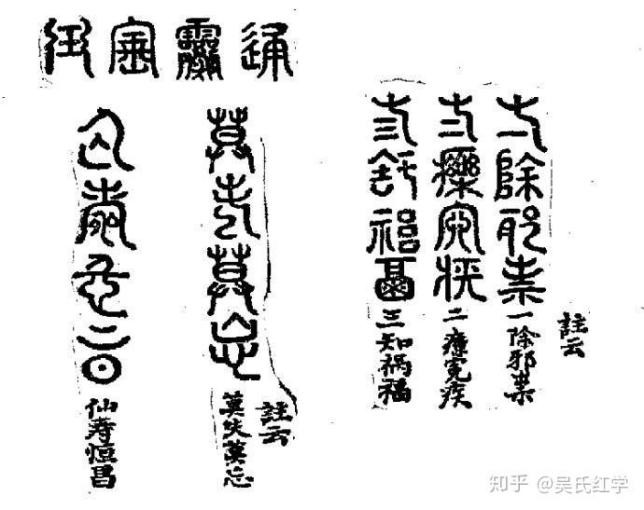
\includegraphics[width=\linewidth ,totalheight=0.95\textheight , keepaspectratio]{tong-ling-bao-yu.jpg}
\end{figure} 
 

宝钗看毕,又从新翻过正面来细看,口内念道:“莫失莫忘,仙寿恒昌。”念了两遍,乃回头向莺儿笑道:“你不去倒茶,也在这里发呆作什么?”莺儿嘻嘻笑道:“我听这两句话,倒像和姑娘的项圈上的两句话是一对儿。”宝玉听了,忙笑说道:“原来姊姐那项圈上也有八个字,我也赏鉴赏鉴。”宝钗道:“你别听他的话,没有什么字。”宝玉笑央:“好姐姐,你怎么瞧我的了呢!”宝钗被他缠不过,因说道:“也是个人给了两句吉利话儿,所以錾上了,叫天天带着;不然,沉甸甸的有什么趣儿!”一面说,一面解了排扣,从里面大红袄上将那珠宝晶莹、黄金灿烂的璎珞掏将出来。宝玉忙托了锁看时,果然一面有四个篆字,两面八字,共成两句吉谶。亦曾按式画下形相:

不离不弃\footnote{伏宝玉弃钗为僧}~芳龄永继\footnote{伏宝钗死}

\begin{figure}[H]
\centering
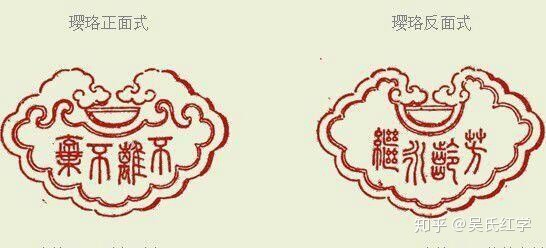
\includegraphics[width=\linewidth ,totalheight=0.95\textheight , keepaspectratio]{fig2.jpg}
\end{figure} 


宝玉看了,也念了两遍,又念自己的两遍,因笑问:“姐姐,这八个字倒真与我的是一对。”莺儿笑道:“是个癞头和尚送的,他说必须錾在金器上......”宝钗不待说完,便嗔他不去倒茶,一面又问宝玉从那里来。

宝玉此时与宝钗就近,只闻一阵阵凉森森、甜丝丝的幽香,竟不知系何香气,遂问:“姐姐熏的是什么香?我竟从未闻见过这味儿。”宝钗笑道:“我最怕熏香,好好的衣服,熏得烟燎火气的!”宝玉道:“既如此,这是什么香?”宝钗想了一想,笑道:“是了,是我早起吃了丸药的香气。”宝玉笑道:“什么丸药这么好闻?好姐姐,给我一丸尝尝!”宝钗笑道:“又混闹了,一个药也是混吃的?”

一语未了,忽听外面人说:“林姑娘来了。”话犹未了,林黛玉已摇摇的走了进来。一见了宝玉,便笑道:“嗳哟,我来的不巧了!”宝玉等忙起身笑让坐。宝钗因笑道:“这话怎么说?”黛玉笑道:“早知他来,我就不来了。”宝钗道:“我更不解这意。”黛玉笑道:“要来时一群都来,要不来一个也不来;今儿他来了,明儿我再来,如此间错开了来着,岂不天天有人来了?也不至于太冷落,也不至于太热闹了。姐姐如何反不解这意思?”

宝玉因见他外面罩着大红羽缎对衿褂子,因问:“下雪了么?”地下婆娘们道:“下了这半日雪珠儿了。”宝玉道:“取了我的斗篷来不曾?”黛玉便道:“是不是?我来了,他就该去了?”宝玉笑道:“我多早晚说要去了?不过是拿来预备着。”宝玉的奶母李嬷嬷因说道:“天又下雪,也好早晚的了,就在这里同姐姐妹妹一处玩玩罢。姨妈那里摆茶果子呢。我叫丫头去取了斗篷来,说给小幺儿们散了罢。”宝玉应允。李嬷嬷出去,命小厮们都各散去不提。

这里薛姨妈已摆了几样细巧茶果,留他们吃茶。宝玉因夸前日在那府里珍大嫂子的好鹅掌、鸭信。薛姨妈听了,忙也把自己糟的取了些来与他尝。宝玉笑道:“这个须得就酒才好。”薛姨妈便命人去灌了些上等的酒来。李嬷嬷便上来道:“姨太太,酒倒罢了。”宝玉笑央道:“好妈妈,我只喝一钟。”李嬷嬷道:“不中用!当着老太太、太太,哪怕你吃一坛呢!想那日我眼错不见一会,不知是那一个没调教的,只图讨你的好儿,不管别人死活,给了你一口酒吃,葬送得我挨了两日骂。姨太太不知道他性子又可恶,吃了酒更弄性。有一日老太太高兴了,又尽着他吃,什么日子又不许他吃,何苦我白赔在里面!”薛姨妈笑道:“老货,你只放心吃你的去。我也不许他吃多了。便是老太太问,有我呢。”一面命小丫鬟:“来!让你奶奶们去,也吃杯搪搪雪气。”那李嬷嬷听如此说,只得和众人且去吃些酒水。这里宝玉又说:“不必烫热了,我只爱吃冷的。薛姨妈忙道:”这可使不得,吃了冷酒,写字手打飐儿。“宝钗笑道:”宝兄弟,亏你每日家杂学旁收的,难道就不知道酒性最热,若热吃下去,发散得就快;若冷吃下去,便凝结在内,以五脏去暖他,岂不受害?从此还不快不要吃那冷的呢!“宝玉听这话有情理,便放下冷的,命人暖来方饮。

黛玉磕着瓜子儿,只抿着嘴笑。可巧黛玉的小丫鬟雪雁走来,与黛玉送小手炉,黛玉因含笑问他说:“谁叫你送来的?难为他费心,那里就冷死了我\footnote{盖冷酒亦喻久亡之人,宝钗劝宝玉不吃冷酒,既有忘却之意,故颦卿不喜也}!”雪雁道:“紫鹃姐姐怕姑娘冷,使我送来的。”黛玉一面接了,抱在怀中,笑道:“也亏你倒听他的话。我平日和你说的,全当耳旁风;怎么他说了你就依,比圣旨还快呢?”宝玉听这话,知是黛玉借此奚落他,也无回复之词,只嘻嘻的笑了两阵罢了。宝钗素知黛玉是如此惯了的,也不去睬他。薛姨妈因道:“你素日身子弱,禁不得冷的,他们记挂着你倒不好?”黛玉笑道:“姨妈不知道。幸亏是姨妈这里,倘或在别人家,人家岂不恼?好说就看得人家连个手炉也没有,巴巴的从家里送个来。不说丫头们太小心过余,还只当我素日是这等轻狂惯了呢。”薛姨妈道:“你这个多心的,有这样想。我就没这样心。”

说话时,宝玉已是三杯过去。李嬷嬷又上来拦阻。宝玉正在心甜意洽之时,和宝、黛姊妹说说笑笑的,那肯不吃。宝玉只得屈意央告:“好妈妈,我再吃两钟就不吃了!”李嬷嬷道:“你可仔细老爷今儿在家,提防问你的书!”宝玉听了这话,便心中大不自在,慢慢的放下酒,垂了头。黛玉先忙的说:“别扫大家的兴!舅舅若叫你,只说姨妈留着呢。这个妈妈,他吃了酒,又拿我们来醒脾了!”一面悄推宝玉,使他赌气;一面悄悄的咕哝说:“别理那老货!咱们只管乐咱们的。”那李嬷嬷也素知黛玉的,因说道:“林姐儿,你不要助着他了。你倒劝劝他,只怕他还听些。”林黛玉冷笑道:“我为什么助着他?我也不犯着劝他。你这妈妈太小心了,往常老太太又给他酒吃,如今在姨妈这里多吃一杯,料也不妨事。必定姨妈这里是外人,不当在这里的也未可知。”李嬷嬷听了,又是急,又是笑,说道:“真真这林姑娘,说出一句话来,比刀子还尖。你这算了什么呢!”宝钗也忍不住笑着,把黛玉腮上一拧,说道:“真真这个颦丫头的一张嘴,叫人恨又不是,喜欢又不是!”薛姨妈一面又说:“别怕,别怕,我的儿!来了这里,没好的你吃,别把这点子东西吓得存在心里,倒叫我不安。只管放心吃,都有我呢!越发吃了晚饭去,便醉了,就跟着我睡罢。”因命:“再烫热酒来!姨妈陪你吃两杯,可就吃饭罢。”宝玉听了,方又鼓起兴来。

李嬷嬷因吩咐小丫头子们:“你们在这里小心着,我家里去换了衣服就来,悄悄的回姨太太,别任他的性,多给他吃。”说着便家去了。这里虽还有三四个婆子,都是不关痛痒的,见李嬷嬷走了,也都悄悄的自寻方便去了。只剩了两个小丫头子,乐得讨宝玉的欢喜。幸而薛姨妈千哄万哄的,只容他吃了几杯,就忙收过了。做了酸笋鸡皮汤,宝玉痛喝了两碗,吃了半碗饭、碧粳粥。一时薛、林二人也吃完了饭,又酽酽的沏上茶来,大家吃了。薛姨妈方放了心。雪雁等三四个丫头已吃了饭,进来伺候。黛玉因问宝玉道:“你走不走?”宝玉乜斜倦眼道:“你要走,我和你一同走。”黛玉听说,遂起身道:“咱们来了这一日,也该回去了。还不知那边怎么找咱们呢。”说着,二人便告辞。

小丫头忙捧过斗笠来,宝玉便把头略低一低,命他戴上。那丫头便将着大红猩毡斗笠一抖,才往宝玉头上一合,宝玉便说:“罢,罢!好蠢东西,你也轻些儿!难道没见过别人戴过的?让我自己戴罢!”黛玉站在炕沿上道:“啰苏什么,过来,我瞧瞧罢!”宝玉忙就近前来。黛玉用手整理,轻轻笼住束发冠,将笠沿掖在抹额之上,将那一颗核桃大的绛绒簪缨扶起,颤巍巍露于笠外。整理已毕,端相了端相,说道:“好了,披上斗篷罢!”宝玉听了,方接了斗篷披上。薛姨妈忙道:“跟你们的妈妈都还没来呢,且略等等不迟。”宝玉道:“我们倒去等他们?有丫头们跟着也够了。”薛姨妈不放心,到底命两个妇女跟随他兄妹方罢。他二人道了扰,一径回至贾母房中。

贾母尚未用晚饭,知是薛姨妈处来,更加喜欢。因见宝玉吃了酒,遂命他自回房去歇着,不许再出来了。因命人好生看侍着。忽想起跟宝玉的人来,遂问众人:“李奶子怎么不见?”众人不敢直说家去了,只说:“才进来的,想有事才去了。”宝玉踉跄回头道:“他比老太太还受用呢,问他作什么!没有他只怕我还多活两日。”一面说,一面来至自己的卧室。只见笔墨在案,晴雯先接出来,笑说道:“好,好!要我研了那些墨,早起高兴,只写了三个字,丢下笔就走了,哄得我们等了一日。快来与我写完这些墨才罢!”宝玉忽然想起早起的事来,因笑道:“我写的那三个字在那里呢?”晴雯笑道:“这个人可醉了!你头里过那府里去,嘱咐我贴在这门斗上的,这会子又这么问。我生怕别人贴坏了,我亲自爬高上梯的贴上,这会子还冻的手僵冷的呢。”宝玉听了,笑道:“我忘了。你的手冷,我替你渥着。”说着便伸手携了晴雯的手,同仰首看门斗上新书的三个字。

一时黛玉来了,宝玉便笑道:“好妹妹,你别撒谎,你看这三个字那一个字好?”黛玉仰头看里间门斗上,新贴了三个字,写着“绛芸轩”。黛玉笑道:“个个都好。怎么写得这么好了?明儿也与我写一个匾。”宝玉嘻嘻的笑道:“又哄我呢。”说着又问:“袭人姐姐呢?”晴雯向里间炕上努嘴。宝玉一看,只见袭人和衣睡着在那里。宝玉笑道:“好!太渥早了些。”因又问晴雯道:“今儿我在那府里吃早饭,有一碟子豆腐皮的包子,我想着你爱吃,和珍大奶奶说了,只说我留着晚上吃,叫人送过来的,你可吃了?”晴雯道:“快别提!一送了来,我知道是我的,偏我才吃了饭,就搁在那里。后来李奶奶来了看见,说:‘宝玉未必吃了,拿来给我孙子吃去罢。’他就叫人拿了家去了。”接着,茜雪捧上茶来。宝玉因让林妹妹吃茶。众人笑说:“林妹妹早走了,还让呢!”

宝玉吃了半碗茶,忽又想起早起的茶来,因问茜雪道:“早起沏了一碗枫露茶,我说过,那茶是三四次后才出色的,这会子怎么又沏了这个来?”茜雪道:“我原是留着的,那会子李奶奶来了,他要尝尝,就给他吃了。”宝玉听了,将手中的茶杯只顺手往地下一掷,"豁啷"一声,打个齑粉,泼了茜雪一裙子的茶。又跳起来问着茜雪道:“他是你那一门子的奶奶,你们这么孝敬他?不过是仗着我小时候吃过他几日奶罢了。如今逞得他比祖宗还大了!如今我又吃不着奶了,白白的养着祖宗作什么!撵了出去,大家干净!”说着,立刻便要去回贾母,撵他乳母。

原来袭人实未睡着,不过故意装睡,引宝玉来怄他顽耍。先闻得说字、问包子等事,也还可不必起来;后来摔了茶钟,动了气,遂连忙起来解释劝阻。早有贾母遣人来问:“是怎么了?”袭人忙道:“我才倒茶来,被雪滑倒了,失手砸了钟子。”一面又安慰宝玉道:“你立意要撵他也好,我们也都愿意出去,不如趁势连我们一齐撵了,我们也好,你也不愁再有好的来服侍你。”宝玉听了这话,方无了言语,被袭人等扶至炕上,脱换了衣服。不知宝玉口内还说些什么,只觉口齿绵缠,眼眉愈加饧涩,忙伏侍他睡下。袭人伸手从他项上摘下那通灵玉来,用自己的手帕包好,塞在褥下,次日带时,便冰不着脖子。那宝玉就枕便睡着了。彼时李嬷嬷等已进来了,听见醉了,不敢前来再加触犯,只悄悄的打听睡了,方放心散去。

次日醒来,就有人回:“那边小蓉大爷带了秦相公来拜。”宝玉忙接了出去,领了拜见贾母。贾母见秦钟形容标致,举止温柔,堪陪宝玉读书,心中十分欢喜,便留茶留饭,又命人带去见王夫人等。众人因素爱秦氏,今见了秦钟是这般人品,也都欢喜,临去时都有表礼。贾母又与了一个荷包并一个金魁星\footnote{作者抚今思昔之事,尚记金魁星乎,令人肠断心摧},取“文星和合”之意。又嘱咐他道:“你家住得远,或一时寒热饥饱不便,只管住在我这里,不必限定了。只和你宝叔在一处,别跟着那起不长进的东西们学。”秦钟一一的答应,回去禀知。

他父亲秦业,现任营缮郎,年近七十,夫人早亡。因当年无儿女,便向养生堂抱了一个儿子并一个女儿\footnote{可知可卿无名无姓,实警幻倩其妹下凡效妲己之务也}。谁知儿子又死了,只剩女儿,小名唤可儿,长大时,生得形容袅娜,性格风流\footnote{贾府重色之风就矣,实乃败家之本}。因素与贾家有些瓜葛,故结了亲,许与贾蓉为妻。那秦业至五旬之上方得了秦钟。因去岁业师亡故,未暇延请高明之士,只得暂时在家温习旧课。正思要和亲家去商议,送往他家塾中去,暂且不致荒废,可巧遇见了宝玉这个机会。又知贾家塾中现今司塾的是贾代儒,乃当今之老儒,秦钟此去,学业料必进益,成名可望,因此十分欢喜。只是宦囊羞涩,那贾家上上下下都是一双富贵眼睛,容易拿不出来;又恐误了为儿子的终身大事,说不得东拼西凑的恭恭敬敬封了二十四两贽见礼,亲自带了秦钟,来代儒家拜见了。然后听宝玉上学之日,好一同入塾。

正是:早知日后闲争气,岂肯今朝错读书\footnote{推颓贾府非但可卿,金钏宝钗等女色齐上阵,连秦钟龙阳断袖都要派上,虎视眈眈警幻苦心可叹}!
 
 
 \chapter{恋风流情友入家塾~起嫌疑顽童闹学堂}
话说秦业父子专候贾家的人来送上学择日之信。原来宝玉急于要和秦钟相遇,却顾不得别的,遂择了后日上学。“后日一早请秦相公到我这里,会齐了,一同前去。”打发人送了去信。

至是日一早,宝玉未起来时,袭人早已把书笔文物包好,收拾停妥,坐在床沿上发闷。见宝玉醒来,只得服侍他梳洗。宝玉见他闷闷的,因笑问道:“好姐姐,你怎么又不自在了?难道怪我上学去丢得你们冷清了不成?”袭人笑道:“这是那里话?读书是极好的事,不然,就潦倒一辈子,终究怎么样呢?但只一件:读书之时只想著书,不读书的时节想着家里些。别和他们一处玩闹,碰见老爷不是玩的。虽说是奋志要强,那工课宁可少些,一则贪多嚼不烂,二则身子也要保重。这就是我的意思,你可要体谅。”袭人说一句,宝玉应一句。袭人又道:“大毛衣服我也包好了,交出给小子们去了。学里冷,好歹想着添换,比不得家里有人照看。脚炉手炉的炭也交出去了,你可着他们添。那一起懒贼,你不说,他们乐得不动,白冻坏了你。”宝玉道:“你放心,出外头我自己都会调停的。你们也别闷死在屋里,长和林妹妹一处去玩笑才好。”说着,俱已穿戴齐备,袭人催他去见贾母、贾政、王夫人等。宝玉又去嘱咐了晴雯、麝月等几句,方出来见贾母。贾母未免也有几句嘱咐他的话。然后去见王夫人,又出来书房中见贾政。

偏生这日贾政回家得早,正在书房中与相公清客们闲话。忽见宝玉进来请安,回说上学里去,贾政冷笑道:“你如果再提‘上学’两字,连我也羞死了。依我的话,你竟玩你的去是正理。仔细站脏了我这地,靠脏了我这门!”众清客相公们都起身笑道:“老世翁何必如此!今日世兄一去,三二年就可显身成名的了,断不似往年仍作小儿之态的。天也将饭时,世兄竟快请罢!”说着便有两个年老的携了宝玉的手走出去了。

贾政因问:“跟宝玉的是谁?”只听外面答应了两声,早进来三四个大汉,打千儿请安。贾政看时,认得是宝玉的奶母之子,名唤李贵的。因向他说道:“你们成日家跟他上学,他到底念了些什么书!倒念了些胡言混语在肚子里,学了些精致的淘气。等我闲一,先揭了你的皮,再和那不长进的算帐!”吓得李贵忙双膝跪下,摘了帽子,碰头有声,连连答应“是”,又回说:“哥儿已念到第三本《诗经》,什么‘呦呦鹿鸣,荷叶浮萍’,小的不敢撒谎。”说的满座哄然大笑起来。贾政也撑不住笑了。因说道:“那怕再念三十本《诗经》,也都是掩耳偷铃,哄人而已。你去请学里师老爷安,就说我说的:什么《诗经》、古文,一概不用虚应故事,只是先把《四书》一齐讲明背熟,是最要紧的。”李贵忙答应“是”,见贾政无话,方退了出去。

此时,宝玉独站在院外,避猫鼠儿似的,屏声静候。待他们出来,便忙忙的走了。李贵等一面掸衣服,一面说道:“可听见了不曾?先要揭我们的皮呢!人家的奴才,跟主子赚些好体面,我们这等奴才,白陪着挨打受骂的。从此后也可怜见些才好。”宝玉笑道:“好哥哥,你别委曲,我明儿请你。”李贵道:“小祖宗,谁敢望你请!只求你听一两句话就有了。”说着,又至贾母这边,秦钟早已来候了,贾母正和他说话儿呢。于是二人见过,辞了贾母。宝玉忽想起未辞黛玉,因又忙至黛玉房中来作辞。彼时黛玉才在窗下对镜理妆,听宝玉未说上学去,因笑道:“好,这一去,可定是要‘蟾宫折桂\footnote{后回宝蟾金桂之事也}’去了。我不能送你了。”宝玉道:“好妹妹,等我下了学再吃晚饭。那胭脂膏子,也等我来再制。”唠叨了半日,方撤身去了。黛玉忙又叫住,问道:“你怎么不去辞辞你宝姐姐呢?”宝玉笑而不答,一径同秦钟上学去了。

原来这贾家之义学,离此不远,不过一里之遥。原系始祖所立,恐族中子弟有贫穷不能请师者,即入此中肄业。凡族中有官爵之人,皆有供给银两,按俸之多寡帮助,为学中之费。特共举年高有德之人为塾掌,专为训课子弟。如今宝、秦二人来了,一一的都互相拜见过,读起书来。自此后,二人同来同往,同坐同起,愈加亲密。又兼贾母爱惜,也时常留下秦钟,住上三天五夜,与自己的重孙一般疼爱。因见秦钟不甚宽裕,又助他些衣履等物。不上一月之工,秦钟在荣府便熟惯了。宝玉终是不安本分之人,一味的随心所欲,因此又发了癖性,又特向秦钟悄说道:“咱俩人一样的年纪,况又同窗,以后不必论叔侄,只论弟兄朋友就是了。”先是秦钟不肯,当不得宝玉不依,只叫他“兄弟”,或叫他的表字“鲸卿”,秦钟也只得混着乱叫起来。

原来这学中虽都是本族人丁与些亲戚的子弟,俗语说得好:“一龙生九种,种种各别。”未免人多了,就有龙蛇混杂,下流人物在内。自宝、秦二人来了,都生得花朵一般模样,又见秦钟腼腆温柔,未语面先红,怯怯羞羞,有女儿之风;宝玉又是天生成惯能作小服低,赔身下气,性情体贴,话语绵缠。因此二人更加亲厚,也怨不得那起同窗人起了疑,背地里你言我语,诟谇谣诼,布满书房内外。

原来薛蟠自来王夫人处住后,便知有一家学,学中广有青年子弟,不免偶动了龙阳之兴。因此,也假说来上学读书,不过是三日打鱼,两日晒网,白送些束修礼物与贾代儒,却不曾有一些进益,只图结交些契弟。谁想这学内就有好几个小学生,图了薛蟠的银钱吃穿,被他哄上手的,也不消多记。更又有两个多情的小学生,亦不知是那一房的亲眷,亦未考其名姓,只因生得妩媚风流,满学中都送了他两个外号,一号“香怜”,一号“玉爱”。虽都有窃慕之意、将不利于孺子之心,只是都惧薛蟠的威势,不敢来沾惹。如今宝、秦二人一来,见了他两个,也不免绻缱羡慕,亦因知系薛蟠相知,故未敢轻举妄动。香、玉二人心中,也一般的留情与宝、秦。因此,四人心中虽有情意,只未发迹。每日一入学中,四处各坐,却八目勾留,或设言托意,或咏桑寓柳,遥以心照,却外面自为避人眼目。不意偏又有几个滑贼,看出形景来,都背后挤眉弄眼,或咳嗽扬声,这也非止一日。

可巧这日代儒有事,早已回家去了,只留下一句七言对联,命学生对了,明日再来上书。将学中之事,又命长孙贾瑞暂且管理。妙在薛蟠如今不大来学中应卯了,因此秦钟趁此和香怜挤眉使暗号,二人假装出小恭,走至后院说梯己话。秦钟先问他:“家里的大人可管你交朋友不管?”一语未了,只听背后咳嗽了一声。二人吓得忙回头看时,原来是窗友名金荣者。香怜本有些性急,便羞怒相激,问他道:“你咳嗽什么?难道不许我们说话不成?”金荣笑道:“许你们说话,难道不许我咳嗽不成?我只问你们:有话不明说,谁许你们这样鬼鬼祟祟的干什么故事?我可也拿住了,还赖什么!先得让我抽个头儿,咱们一声儿不言语,不然大家就奋起来。”秦、香二人急得飞红了脸,便问道:“你拿住什么了?”金荣笑道:“我现拿住了是真的。”说着,又拍着手笑嚷道:“贴的好烧饼!你们都不买一个吃去?”秦钟、香怜二人又气又急,忙进来向贾瑞前告金荣,无故欺负他两个。

原来这贾瑞最是个图便宜,没行止的人,每在学中以公报私,勒索子弟们请他;后又附助着薛蟠图些银钱酒肉,一任薛蟠横行霸道,他不但不去管约,反助纣为虐讨好儿。偏那薛蟠本是浮萍心性,今日爱东,明日爱西,近来又有了新朋友,把香、玉二人丢开一边。就连金荣亦是当日的好朋友,自有了香、玉二人,便弃了金荣。近日连香、玉亦已见弃。故贾瑞便无了提携帮衬之人。他不说薛蟠得新弃旧,只怨香、玉二人不在薛蟠前提携帮补他,因此贾瑞、金荣等一干人,正在醋妒他两个。今见秦、香二人来告金荣,贾瑞心中便不自在起来,虽不好呵叱秦钟,却拿着香怜作法,反说他多事,着实抢白了几句。香怜反讨了没趣,连秦钟也讪讪的各归坐位去了。金荣越发得了意,摇头咂嘴的,口内还说许多闲话,玉爱偏又听了不忿,两个人隔座咕咕唧唧的角起口来。金荣只一口咬定说:“方才明明的撞见他两个在后院里亲嘴摸屁股,两个商议定了,一对一肏,撅草根儿抽长短,谁长谁先干。”金荣只顾得意乱说,却不防还有别人。谁知早又触怒了一个。你道这个是谁?

原来这一个名唤贾蔷,亦系宁府中之正派玄孙,父母早亡,从小儿跟着贾珍过活,如今长了十六岁,比贾蓉生的还风流俊俏。他弟兄二人最相亲厚,常相共处。宁府人多口杂,那些不得志的奴仆们,专能造言诽谤主人,因此,不知又有了什么小人诟谇谣诼之词。贾珍想亦风闻得些口声不大好,自己也要避些嫌疑,如今竟分与房舍,命贾蔷搬出宁府,自去立门户过活去了。这贾蔷外相既美,内性又聪明,虽然应名来上学,亦不过虚掩眼目而已。仍是斗鸡走狗,赏花玩柳。总恃上有贾珍溺爱,下有贾蓉匡助,因此族人谁敢来触逆于他。他既和贾蓉最好,今见有人欺负秦钟,如何肯依?自己要挺身出来抱不平,心中且又忖度一番,:“金荣、贾瑞一干人,都是薛大叔的相知,向日我又与薛大叔相好,倘或我一出头,他们告诉了老薛,我们岂不伤了和气?待要不管,如此谣言,说得大家没趣。如今何不用计制伏,又止息口声,又不伤脸面?”想毕,也装作出小恭,走至外面,悄悄把跟宝玉的书童名唤茗烟者唤到身边,如此这般,调拨他几句。

这茗烟乃是宝玉第一个得用的,且又年轻不谙世事,如今听贾蔷说金荣如此欺负秦钟,连他的爷宝玉都干连在内,不给他个利害,下次越发狂纵难制了。这茗烟无故就要欺压人的,如今听了这话,又有贾蔷助着,便一头进来找金荣。也不叫金相公了,只说“姓金的,你是什么东西!”贾蔷遂跺一跺靴子,故意整整衣服,看看日影儿说:“是时候了。”遂先向贾瑞说有事要早走一步。贾瑞不敢强他,只得随他去了。这里茗烟先一把揪住金荣问道:“我们肏屁股不肏,管你鸡(原字为左毛右几)巴(原字为左毛右巴)相干!横竖没肏你爹去就罢了你是好小子,出来动一动你茗大爷!”吓得满屋中子弟都怔怔的痴望。贾瑞忙吆喝:“茗烟不得撒野!”金荣气黄了脸,说:“反了,反了!奴才小子都敢如此,我只和你主子说。”便夺手要去抓打宝玉、秦钟。尚未去时,从脑后飕的一声,早见一方砚瓦飞来\footnote{好笑之极},并不知系何人打来的,幸未打着,却又打在旁人的座上,这座上乃是贾蘭、贾菌。

这贾菌\footnote{木死生菌,暗指家亡人尽也}亦系荣国府近派的重孙,其母亦少寡,独守着贾菌。这贾菌与贾蘭最好,所以二人同桌而坐。谁知贾菌年纪虽小,志气最大,极是个淘气不怕人的。他在座上冷眼看见金荣的朋友暗助金荣,飞砚来打茗烟,偏没打着茗烟,便落在他桌上,正打在面前,将一个磁砚水壶打了个粉碎,溅了一书黑水。贾菌如何依得,便骂:“好囚攮的们,这不都动了手了么!”骂着,也便抓起砚砖来要打回去。贾蘭是个省事的\footnote{何为省事?蘭即阑珊也,尽也,故言省事一笑},忙按住砚,极口劝道:“好兄弟,不与咱们相干。”贾菌如何忍得住,便两手抱起书匣子来,照那边抡了去。终是身小力薄,却抡到半道,至宝玉、秦钟桌案上就落了下来。只听"豁啷啷"一声响,砸在桌上,书本、纸片、笔砚等物撒了一桌,又把宝玉的一碗茶也砸得碗碎茶流。贾菌便跳出来,要揪打那一个飞砚的。金荣此时随手抓了一根毛竹大板在手,地狭人多,那里经得舞动长板。茗烟早吃了一下,乱嚷道:“你们还不来动手?”宝玉还有三个小厮:一名锄药,一名扫红,一名墨雨。这三个岂有不淘气的,一齐乱嚷:“小妇养的!动了兵器了!”墨雨遂掇起一根门闩,扫红、锄药手中都是马鞭子,蜂拥而上。贾瑞急得拦一回这个,劝一回那个,谁听他的话,肆行大闹。众顽童也有趁势帮着打太平拳助乐的,也有胆小藏过一边的,也有直立在桌上拍着手儿乱笑,喝着声儿叫打的。登登间鼎沸起来。

外边李贵等几个大仆人听见里边作起反来,忙都进来,一齐喝住。问是何原故,众声不一,这一个如此说,那一个又如彼说。李贵且喝骂了茗烟等四个一顿,撵了出去。秦钟的头早撞在金荣的板子上,打起一层油皮,宝玉正拿褂襟子替他揉呢,见喝住了众人,便命李贵:“收书!拉马来,我去回太爷去!我们被人欺负了,不敢说别的,守礼来告诉瑞大爷,瑞大爷反倒派我们的不是,听着人家骂我们,还调唆他们打我们。茗烟见人欺负我,他岂有不为我的?他们反打伙儿打了茗烟,连秦钟的头也打破了,这还在这里念什么书!茗烟他也是为有人欺侮我的。不如散了罢。”李贵劝道:“哥儿不要性急。太爷既有事回家去了,这会子为这点子事去聒噪他老人家,倒显得咱们没理似的。依我的主意,那里的事情那里了结,何必惊动老人家。这都是瑞大爷的不是,太爷不在这里,你老人家就是这学里的头脑了,众人看你行事。众人有了不是,该打的打,该罚的罚,如何等闹到这步田地还不管?”贾瑞道:“我吆喝着都不听。”李贵笑道:“不怕你老人家恼我,素日你老人家到底有些不正经,所以这些兄弟才不听。就闹到太爷跟前去,连你老人家也脱不过的。还不快作主意撕罗开了罢!”宝玉道:“撕罗什么?我必是回去的!”秦钟哭道:“有金荣,我是不在这里念书的。”宝玉道:“这是为什么?难道有人家来得,咱们倒来不得?我必回明白众人,撵了金荣去。”又问李贵:“金荣是那一房的亲戚?”李贵想一想道:“也不用问了。若说起哪一房的亲戚,更伤了兄弟们的和气。”

茗烟在窗外道\footnote{金荣之荣同茗烟之化烟恰是一对}:“他是东胡同子里璜大奶奶的侄儿。哪是什么硬正仗腰子的,也来唬我们!璜大奶奶是他姑娘。你那姑妈只会打旋磨子,给我们琏二奶奶跪着借当头。我眼里就看不起他那样的主子奶奶!”李贵忙断喝不止,说:“偏你这小狗肏的知道,有这些蛆嚼!”宝玉冷笑道:“我只当是谁的亲戚,原来是璜嫂子的侄儿,我就去问问他来!”说着便要走。叫茗烟进来包书。茗烟包著书,又得意道:“爷也不用自己去见,等我去他家,就说老太太有说的话问他呢,雇上一辆车拉进去,当着老太太问他,岂不省事?”李贵忙喝道:“你要死!仔细回去我好不好先捶了你,然后再回老爷、太太,就说宝玉全是你调唆的。我这里好容易劝哄好了一半,你又来生个新法子。你闹了学堂,不说变法儿压息了才是,倒要往大里闹!”茗烟方不敢作声儿了。

此时,贾瑞也生恐闹大了,自己也不干净,只得委曲着来央告秦钟,又央告宝玉。先是他二人不肯。后来宝玉说:“不回去也罢了,只叫金荣赔不是便罢。”金荣先是不肯,后来禁不得贾瑞也来逼他去赔不是,李贵等只得好劝金荣,说:“原是你起的端,你不这样,怎得了局?”金荣强不过,只得与秦钟作了揖。宝玉还不依,偏定要磕头。贾瑞只要暂息此事,又悄悄的劝金荣说:“俗语说得好:‘杀人不过头点地。’你既惹出事来,少不得下点气儿,磕个头就完事了。”金荣无奈,只得进前来与秦钟磕头。贾瑞遂立意要去调拨薛蟠来报仇,与金荣计议已定。一时散学,各自回家。不知他怎么去调拨薛蟠?且听下回分解。



\chapter{金寡妇嗔姤凝曦轩~秦可卿淫上天香楼}
话说金荣因人多势众,又兼贾瑞勒令,赔了不是,给秦钟磕了头,宝玉方才不吵闹了。大家散了学,金荣回到家中,越想越气,说:“秦钟不过是贾蓉的小舅子,又不是贾家的子孙,附学读书,也不过和我一样,他因仗着宝玉和他好,他就目中无人。他既是这样,就该行些正经事,人也没的说,他素日又和宝玉鬼鬼祟祟的,只当我们都是瞎子,看不见。今日他又去勾搭人,偏偏的撞在我眼里,就是闹出事来,我还怕什么不成?”他母亲胡氏听见他咕咕嘟嘟的说,因问道:“你又要争什么闲气?好容易我望你姑妈说了,你姑妈千方百计的才向他们西府里的琏二奶奶跟前说了,你才得了这个念书的地方。若不是仗着人家,咱们家里还有力量请的起先生?况且人家学里,茶也是现成的,饭也是现成的。你这二年在那里念书,家里也省好大的嚼用呢。省出来的,你又爱穿件鲜明衣服。再者,不是因你在那里念书,你就认得什么薛大爷了?那薛大爷一年不给不给,这二年也帮了咱们有七八十两银子\footnote{因何无故给许多银子?金母亦当细思之。}。你如今要闹出了这个学房,再要找这么个地方,我告诉你说罢:比登天还难呢!你给我老老实实的顽一会子睡你的觉去,好处多着呢!”于是金荣忍气吞声,不多一时,他自去睡了。

次日仍旧上学去了。一大早进了学堂,因昨日给人跪下赔不是,脸上无光,垂头丧气躲在屋后花园撕树条子闲掷。只见薛蟠同贾蓉解手打茅厕里出来,两个叽叽咕咕的,忽看见金荣哭丧着脸躲着发闷。薛蟠走来笑道:“小荣儿今儿怎么了,看见人也不招呼一声,是谁欺负你了,我替你报仇。”金荣抬眼不语,头扭到一边。贾蓉一边低声道:“大哥昨日没来,不知道发生了天大的事故,有人打你兄弟了。他现在正烦着呢。”薛蟠眼瞪的铜铃一般道:“竟有此事,谁敢欺负我兄弟,他不想活了?快告诉我是谁。”贾蓉在他耳边细细说了昨日之事,金荣撇撇嘴道:“薛大哥就忍下这口气吧,他们都是仗着府里有头有脸的,抢大哥的朋友,谁敢不从。以后不过任着他们欺负罢了。”薛蟠因有了新朋友,早把金荣丢开。本不想管这样的事,谁想贾蓉耳边调唆是宝玉同他抢秦钟,使秦钟时时不能沾手,不觉登然大怒,骂道:“秦钟这小子反了,他算那根葱,我这就找他评理,我打不死他。”金荣、贾蓉假意笑着去拉,被薛蟠一挣手甩开了。

薛蟠大步流星奔入学堂,恰见秦钟、宝玉、茗烟、贾瑞、贾蔷俱在内,指着茗烟鼻子骂道:“你小子敢打我的兄弟,反了天了,今日不打你个脑袋开花,我不姓薛。”上来便要打人,茗烟唬的躲到墙角。宝玉拿身子挡着他,喝道:“是你的兄弟先滋衅撩事,不可鲁莽。”贾瑞、贾蔷笑着上前拉劝,道:“过去了何必再提,大家放开手罢。”薛蟠不依,拿书本望茗烟头上投去,刚巧砸在贾菌额上。薛蟠又上去抓取秦钟,两个撕扯起来。薛蟠骂道:“我待你那一刻不尽心,天天见我就躲,像个避猫鼠,他们都是好的,就我不好了,你打我兄弟此是一,你勾引宝兄弟就罢了,为何连我的香怜都去抢?看我打不死你。”秦钟喘息辩道:“薛大哥错误了,我何时勾搭过他们。”薛蟠上去掐他的脖子,宝玉气的嚷道:“薛大哥也不顾这边的情义只管打人,回去我告诉宝姐姐去。”薛蟠听了如醍醐灌顶,不觉垂下头来,一身不吭回自己座位上坐了。大家都东张西望不敢言语。 

且说金荣姑妈,原聘给的是贾家玉字辈的嫡派,名唤贾璜,但其族人那里皆能象宁荣二府的富势?原不用细说。这贾璜夫妻守着些小的产业,又时常到宁荣二府里去请安,又会奉承凤姐儿并尤氏,所以凤姐儿尤氏也时常资助资助他,方能如此度日。今日正遇天气晴明,又值家中无事,遂带了一个婆子,坐上车,来家里走走,瞧瞧寡嫂并侄儿。闲话之间,金荣的母亲偏提起昨日贾家学房里的那事,从头至尾,一五一十都向他小姑子说了。这璜大奶奶不听则已,听了一时怒从心上起,说道:“这秦钟小崽子是贾门的亲戚,难道荣儿不是贾门的亲戚?人都别忒势利了!况且都作的是什么有脸的好事!就是宝玉,也犯不上向着他到这个样。等我去到东府瞧瞧我们珍大奶奶,再向秦钟他姐姐说说,叫他评评这个理!”这金荣的母亲听了这话,急的了不得,忙说道:“这都是我的嘴快,告诉了姑奶奶了。求姑奶奶别去,别管他们谁是谁非。倘或闹起来,怎么在那里站得住?若是站不住,家里不但不能请先生,反倒在他身上添出许多嚼用来呢!”璜大奶奶听了,说道:“那里管得许多?你等我说了,看是怎么样。”也不容他嫂子劝,一面叫老婆子瞧了车,就坐上往宁府里来。

到了宁府,进了车门,到了东边小角门前下了车,走了一会子,因怕遇见贾珍,只是找秦可卿论理,脚步错乱,不觉来到会芳园,看见远远有个临水所建轩堂,上头题着凝曦轩,身子乏的很,便进去歇歇脚。忽见贾珍之妻尤氏打那边过来,一脸怒色,身旁跟着两个丫头。金氏听闻尤氏是贾珍原配夫人死后续娶的继室,贾蓉不是他的亲生,如今是个当家人,金氏躲在柱后,偷偷地看他们往那边走远了,才喘了一口气坐在石凳上。不大会儿,只见贾珍两个侍妾佩凤偕鸳走了进来,慌忙迎上去施礼,未敢气高,殷殷勤勤叙过寒温,说了些闲话,方问道:“今日怎么没见蓉大奶奶?”佩凤说到:“他这些日子病了,在家里歪着,懒待动,话也懒待说,眼神也发眩。静静的养病。本来就病的不轻,又气他兄弟不学好,不上心念书,以致学里吵闹。今日索性连早饭也没吃。姐姐要替他找个好大夫呢。”金氏听了这半日话,知道秦氏也为学堂里的事情生气,且又病了,把方才在他嫂子家的那一团要向秦氏理论的盛气,早吓的都丢在爪洼国去了。心内想道:“才刚看见尤氏一脸怒气,想是也为他兄弟的事着恼,他又病着,何必在这节骨眼上寻人是非,来到不是时候,还是回去方是。”乃对佩凤二人笑道:“听闻宁府里花园里有几样花儿盛开,我赶来赏花,谁知并无这样事,是听几个奴才说谎,倒也扫兴,我也该回去了。”于是拜辞二位,悻悻的走了。佩凤见他走了,笑道:“此人说了一大通,却不大认识,想是那府里的管事的。”偕鸳道:“我也不认识,先别管他,你说尤姐姐这会子怒气冲冲是去往那里,好好的怎么恼起来了。”佩凤道:“我也不知。”又左右看看没人,悄悄地道:“这里有个缘故,兴许他是为这事着恼呢。”偕鸳道:“不妨说说看。”佩凤道:“咱也不是爱搬弄是非的人,我也是听人说的,他儿媳妇有几个头了。”偕鸳道:“这也太唬人了,一个还不够,还有好几个。”佩凤道:“珍大爷是个吃着碗里看着锅里的,那日他在我屋里睡了,喝的醉醺醺的,夜里老是念叨着他儿媳妇的名字,白天起来他又失魂落魄的说府里没见过像他儿媳妇这样温柔娇媚的。我忖度着他定是看上他儿媳妇了。怪不得他夫人生气呢。”偕鸳道:“可是胡说,那有老公公爱他儿媳妇的。不想和你说了,越发没个捆了。”佩凤道:“妹妹怎么恼了,你不信我的话,就没看见珍大爷天天往他儿媳妇屋里嘘寒问暖吗,他儿媳妇生的比别人好些,时常见蔷哥儿来他家寻蓉儿吃酒,与他眉来眼去的,不免人不起疑。”偕鸳道:“好没意思的话,不想说了,咱们走罢。”佩凤笑了笑起身同他走了。

且说尤氏一大早听家里老婆子说秦可卿那日容留宝玉睡他屋里,便有了心,叫了老婆子问个究竟。那嬷嬷道:“老身与他说了,那里有个叔叔往侄儿房里睡觉的理,他反笑着说,他能多大呢,就忌讳这些个。我就不说了,等好大会儿我进去看时,看到小哥儿裤子都湿了,只当他尿床了,正要替他找个裤子换上,却见他那里黏黏糊糊的不象是尿床,心里明白了大半。忽听小丫头议论说,他们偷看到你儿媳妇拿手替小哥儿打手铳,我想虽不是个事儿,可终不免有些猥亵,兴许是小丫头看花了眼,他是在帮小哥儿盖被子呢。若是如此,这些小丫头也是该死,岂有胡说乱道的。”尤氏听了,心内一沉,思到:“小丫头绝不会非议主子,定是儿媳妇见宝玉生的俊俏,禁不住做了不耻之事。”可又不好寻他是问,心里生闷气,一脸怒色出门去了。

秦氏见婆婆一大早说话不兴头,拿些硬话塞责,有些纳闷,也不放在心上。自从上回贾蔷来约蓉儿吃酒,见他生的风流俊俏,便有些心猿意马,不时拿语言撩拨他,贾蔷是个明白人,见他有意沾惹,且生的风流袅娜,不免心驰神往起来。渐渐两人一来一往,背地里也私约密盟,在天香楼\footnote{天香楼原名“西帆楼”,因西字触动往事,读之令人酸鼻,因命雪芹改名天香楼。}宽衣解带,肌肤相亲几回。幸喜无人察觉,两人意犹未尽,他日再约。秦氏是个风流成性的人,看见俊俏后生就眉目传情,不肯放过,宁府有几个小厮因容貌清俊,纯朴可爱,也渐入美人眼,肆意套取,那些人都是年轻气盛,未沾惹过女色,有佳人自主投怀送抱,恰似苍蝇闻臭蚊子见血,岂有推辞不依的,就算刀架在脖子上,也要风流一回。秦氏越发放荡淫靡起来,恨不得把府中大大小小所有壮夫英汉俱纳归石榴裙下。这也是冤孽相逢,人以类聚。这日贾蓉不在家,贾蔷与秦氏暗暗密约中午过后在天香楼再续好事,秦氏在自己房里放置木盆,柔抿蝉鬓,镜擦朱唇,金钗轻解,云鬓泻下,熏香洗浴而待,心腹小丫头瑞珠在门口戏耍把守。谁知贾珍在外今日多饮几杯,趔趔趄趄赶回来嚷道:“蓉儿那里去了,他眼里越发没有我这个当老子的了。”下人回禀道:“蓉大爷往街上买笔墨纸砚习学去了。”贾珍道:“这小子那里知道读书,定是躲屋里不肯见我。”乃往贾蓉房里找儿子训话,经过秦氏门口,闻见一阵脂皂香气,甚是怡人,见房门紧闭,听见里面有撩水泼洗之声,便知是儿媳妇在洗浴,心里突突直跳,一把推开房门,却见里面热气腾腾,水气弥漫,秦氏坐在木桶里正在泼水揉搓。贾珍见他纤手清香琼珠溅,香肌雪肤体态娇,两瓣金莲躺床脚,一袭云纱倚枕头,不觉心荡魂摇,淫念愈炽,恨不得抢步上去携玉手,揽蛇腰,抱佳人纱帐内以畅其美。秦氏大惊,脱口而出道:“你进来作甚?还不退了出去。”贾珍红晕着脸颊摇摇晃晃道:“好一幅午后香浴图。”上来就去抓摸与他。秦氏哀告推揉,一手扳着盆沿,不肯起来。贾珍笑道:“美人依了我罢。”秦氏怒道:“岂有此理,老公公要菲薄儿媳妇,这是那家的道理。”贾珍不觉心里一惊,自责道:“我是老糊涂了,怎么打起儿媳妇主意来了。我不是人,我该死。”说完转身要走。秦氏见他生的肩宽背阔,面目老成英武,目光邪淫,别有一番风情,不觉含嗔姣喘道:“门外没有人,你把门闩扣上罢。”贾珍惑然不解。秦氏含羞笑道:“还不过来替我涂脂擦背。”贾珍片刻迟疑,赶去插上门闩,转身过来坐在盆边,拿水撩他身上,秦氏回头莞尔一笑,抓住其手为自己揉搓,贾珍咽下口水,正要施为,忽听门外瑞珠急促喊道:“夫人,蔷大爷来找蓉大爷了。”二人一惊,不知所措,贾珍急忙放手起身打开门闩,匆忙溜了出去。

话说贾蔷赶来赴约,喜气盈腮,却见贾珍迎了出来。愕然笑道:“老爷不是在十里街吃酒聚友吗,怎么回来了。”贾珍笑道:“你是来找蓉儿的罢,他往街上买纸笔去了,进来坐坐罢。”贾蔷笑道:“也没什么大事,就是薛大哥想请蓉哥吃酒,要我来找他。既然他不在家,我改日再来找他。薛大哥在那边还在等我回话,我就不逗留了,告辞。”贾珍笑道:“也好,等蓉儿回来,我告与他知道。”因命小厮送客。贾蔷笑着摆手道:“不必了,我先行一步。”匆忙走了。贾珍目送他走远了,急忙赶回来去找秦氏,却见秦氏已经穿戴齐整,上前懊悔道:“我多喝了几杯,竟然做起胡涂事来,实在惭愧。”秦氏笑道:“老爷不必自愧,做儿媳的伺候老爷是应当的,有话就请说,不必客气。”贾珍不语。秦氏低声道:“这里人多眼杂,我立刻要去天香楼厕间更衣,那里没人,你到楼上看看焦大打扫的怎么样了。”说完命瑞珠跟着出去了。贾珍会意,见无人旁听,也匆促走了出去。

贾珍赶到天香楼下,却见焦大嘟嘟囔囔打扫落叶,乃肃色道:“近来听闻有人抱怨说奴才打扫懒惰,我故来查看,汝等不可懈怠,把楼下再打扫一遍,我上楼检视一番。”说完快步上楼去了。焦大看他上去了,往地上吐了一口,慢慢的扫着芥灰。贾珍到了厕间,找不到秦氏,只见瑞珠向他招手。贾珍喜冲冲进了室内,看见里头停一床榻,秦氏歪在榻上,粉面含羞笑而不语。瑞珠退了出去。贾珍上前揽肩擦面,两人卿卿我我,云雨一番,好不惬意。   

从此二人多次天香楼聚约淫会,被奴仆察觉,不觉起了疑。焦大暗想:“时常有贾蔷同他私会,怎么老公公也来了,着实令人不解。”怂恿小厮上楼偷窥,看见二人你亲我爱云翻雨滚,吃了一惊不小,下来告与焦大知晓。焦大讳奸如仇,怒怨生厌,逢人便说,一传十十传百,风声渐渐地传到众人耳里。

也是合该有事。一日,贾珍秦氏天香楼偷欢回来,不慎丢落一枝金簪于房内。秦氏丫鬟宝珠上楼晒衣裳,忽然捡到此簪,是一枝蝶穿银花绞丝发簪,认出是秦氏之物,心想:“定是夫人上楼如厕丢落,若占为己有,人人皆知系夫人之物,吾必吃盗窃官司。谨而慎之,还是上缴讨好主子得个好名声为妙。”乃兴冲冲赶来寻找秦氏。在厅堂遇见尤氏,忙垂首施拜。尤氏见他手里拿着簪子,笑道:“你拿着主子的簪子作甚,去典当行不成?”宝珠忙道:“这是我刚刚捡到的,正要交给夫人呢。”尤氏拿过簪子打量道:“我认得这个,是你主子戴的,你是打那里捡的?”宝珠笑道:“我往天香楼晒夫人的衣裳,在楼上厕房捡的。”尤氏时时听到府中奴才偷偷议论秦氏与丈夫的风言风语,不足为信。今日看到簪子,也起了疑心,心想:“如厕何必去天香楼,近处就有茅厕,定有玄机。”又想起秦氏那日替宝玉打手铳,已是怀怨,知媳妇不是正经人,不曾想媳妇竟然与老公公爬灰,此乃天地不容的丑事,岂能不管不问。于是怒气冲冲持簪去找丈夫理论,只见贾蓉进来,心生一计,对他道:“蓉儿过来,有话给你说。”贾蓉笑道:“太太不妨道来。”尤氏道:“宝珠出去!”宝珠应了一声退下。尤氏便说秦氏在天香楼丢落簪子一个。贾蓉道:“太太有何深意?”尤氏道:“近来口声不好,家里十停人倒有五停人说你媳妇与老公公在天香楼不干不净的,我犹不信。今儿看见这个,我也疑心不小,你看此事如何了解。”贾蓉夜里也曾听见秦可卿梦里唤父亲的名字,心里纳罕,听尤氏这般说,心里升腾起一股怒气,道:“今日定去天香楼捉奸,看他们怎么说。”乃与尤氏偷偷商议起来。中午过后,尤氏借口去探望老太太,携小丫头走了。贾蓉说薛蟠要他去街上帮忙看视古扇鸟雀,要晚间回来,也急匆匆走了。秦氏要瑞珠去探贾珍递暗号儿,贾珍欢天喜地赶来,两个相约再去天香楼欢聚,分头去了。

且说尤氏、贾蓉躲藏天香楼下耳房内,忽见焦大持帚走来急声道:“他们已经上楼多时,是时候了。”尤氏贾蓉推门出来,快步登楼,却见瑞珠守在楼梯打盹。二人脚步声惊醒瑞珠,唬的他急忙往楼上赶,被贾蓉打了一记耳光。尤氏到各个房间寻找,果见贾珍秦氏在房里赤裸相抱。尤氏上去打了这个又打那个,口里骂不绝口。贾蓉也窜了进来,看见这番丑态,按到秦氏挥拳就打。贾珍怒喝推揉贾蓉道:“小子无礼,还不住手。”反挥手去打贾蓉。贾蓉推贾珍道:“你们做出这种人神共愤天地不齿的事,家里的名声都被你们带坏了,我以后还怎么见人。”贾珍吼道:“什么大不了的,我再给你娶一房就是了。”尤氏哭嚷道:“这也是你做老公公说的话?我如今也不要脸了,定要告诉大家知道,看看儿媳妇与老公公都是怎么做人的。”说完掩口哭着跑了出去。贾蓉急忙去追。贾珍秦氏一脸颓丧,面面相觑。两个慌乱穿衣整袂,赶了出去。秦氏不觉晕倒在地,贾珍一行扶一行喊瑞珠过来帮忙。

且说尤氏哭哭啼啼回去,不好独承此事,把天香楼一事告与邢夫人。邢夫人听了大怒,喝道:“这还了得。”又去找王夫人。王夫人正与贾母说笑儿,看见邢夫人来了,要他好生坐了。邢夫人见没有旁人,冷笑道:“咱们贾家以后可没脸见人了,祖宗的颜面也不要了。”贾母惊讶道:“贤媳何出此言,又为何事而来。”王夫人也诧然望着他。邢夫人乃把天香楼捉奸一事细细说了,贾母听了,差点没有背过气去,喘吁吁道:“天神老爷,我也不活了,谁承望生下这样不肖的孽障。”不禁老泪纵横。王夫人惊诧道:“这样伤风败俗的事,须告诉大老爷,老爷知道。”贾母捶胸顿足道:“那孩子我平日看他温柔懂事,谁曾想竟是这样一个人,白辜负了我的心,我白疼了他一场,赶快把他送回他父亲那里去,我不能瞧。”王夫人道:“他父亲早归天了,家里没有人了。”邢夫人冷笑道:“如此不齿之事,就这样轻易打发回家了,焉能服众。”贾母气的心窝疼,王夫人急忙唤鸳鸯上来,搀扶贾母回去了。邢夫人怒道:“快把珍儿那个孽障叫来,他父亲不管他,我替他教训儿子。”下人答应一声去了。一会回来禀报:“珍大爷抱病不愿来,在家静养呢。”邢夫人更是气的目眦发直。尤氏回到宁府,忿犹未尽,闯入秦氏房内口角,只见秦氏躺在床上,宝珠端着茶碗,拿着汤匙给他喂药。一回头看见尤氏进来了,笑道:“太太来了。奶奶病了,昨夜翻来覆去睡不着,身上烫的厉害。”尤氏撇嘴一声不吭出去了。秦氏见婆婆走了,满脸是泪哭道:“我这病怕是治不好了,我还是死了罢。”宝珠不解道:“奶奶是怎么了?”秦氏泣道:“你不懂,快去看看瑞珠在那里,我要见他。”宝珠答应了去找瑞珠。不大会儿进来了,说道:“蓉大爷在院里叫了几个小厮捆绑了瑞珠,说要关马棚里。老爷骂他儿子,不要他捆,正在呵斥儿子呢。蓉大爷拗不过,只得放了瑞珠,老爷把瑞珠带走了。”秦氏叹道:“是我连累了他,我有罪。”宝珠听不明白,心里盘算半天,不知所以然。


 
\chapter{怀愧女迎阻宁国府~不伦子欲接天台路}
话说秦可卿同贾珍的孽情经焦大口口相传,弄得人尽皆知了,贾母听闻其事,气的饭都不吃。一个人在房里怄气,鸳鸯哄他吃了几口,问他因何不乐,贾母道:“我气这些孩子不听话不学好。”鸳鸯也不吱声了。秦可卿本来身上有病,这回愈发加重了,贾珍派人给他抓药,吃了也不见好,秦可卿是心里羞愧致病,药力难以企及,尤氏也不理他,逢人便说他病了。是日贾敬的寿辰,贾珍先将上等可吃的东西,稀奇些的果品,装了十六捧盒,着贾蓉带领家下人等与贾敬送去,向贾蓉说道:“你留神看太爷喜欢不喜欢,你就行了礼来。你说:‘我父亲遵太爷的话未敢来,在家里率领合家都朝上行了礼了。’”贾蓉听罢,即率领家人去了。

尤氏也跟了出去,要交代他几句,只见秦可卿懒懒的过来了,尤氏皱眉道:“老太太、太太他们在里面,你就不要进去了,近来风声不好,他们看见你也烦心。”秦可卿本来心里有愧,不愿面见众人,可人人都来他不来,怕违了礼数,谁知婆婆当面撵他,心里一酸,差点掉下泪来,急忙弯腰拜辞,转身掩口抽抽噎噎而去。尤氏、贾蓉面有嗔色望着他走远了,才转身回来。 

这里渐渐的就有人来了。先是贾琏、贾蔷到来,先看了各处的座位,并问:“有什么玩意儿没有?”家人答道:“我们爷原算计请太爷今日来家,所以并未敢预备顽意儿。前日,听见太爷又不来了,现叫奴才们找了一班小戏儿并一档子打十番的,都在园子里戏台上预备着呢。”次后邢夫人、王夫人、凤姐儿、宝玉都来了,贾珍并尤氏接了进去。尤氏的母亲已先在这里呢。大家见过了,彼此让了坐。贾珍、尤氏二人亲自递了茶,因笑说道:“老太太原是老祖宗,我父亲又是侄儿,这样日子,原不敢请他老人家;但是这个时候,天气正凉爽,满园的菊花又盛开,请老祖宗过来散散闷,看着众儿孙热闹热闹,是这个意思。谁知老祖宗又不肯赏脸。”凤姐儿未等王夫人开口,先说道:“老太太昨日还说要来着呢,因为晚上看着宝兄弟他们吃桃儿,老人家又嘴馋了,吃了有大半个,五更天的时候,就一连起来了两次,今日早晨略觉身子倦些。因叫我回大爷,今日断不能来了,说有好吃的要几样,还要很烂的。”贾珍听了笑道:“我说老祖宗是爱热闹的,今日不来,必定有个原故,若是这么着就是了。”王夫人道:“前日听见你大妹妹说,蓉哥儿媳妇儿身上有些不大好,到底是怎么样?”尤氏道:“他这个病病得也奇,上月中秋还跟着老太太、太太们玩了半夜,回家来好好的。到了二十后,一日比一日觉懒,也懒待吃东西,这将近有半个多月了。经期又有两个月没来。”邢夫人接着说道:“别是喜罢?”

正说着,外头人回道:“大老爷、二老爷并一家子的爷们都来了,在厅上呢。”贾珍连忙出去了。这里尤氏方说道:“从前大夫也有说是喜的。昨日冯紫英荐了他从学过的一个先生,医道很好,瞧了说不是喜,竟是很大的一个症候。昨日开了方子,吃了一剂药,今日头眩得略好些,别的仍不见怎么样大见效。”凤姐儿道:“我说他不是十分支持不住,今日这样的日子,再也不肯不扎挣着上来。”尤氏道:“你是初三日在这里见他的,他还强扎挣了半天,也是因你们娘儿两个好的上头,他才恋恋的舍不得去。”凤姐儿听了,眼圈儿红了半天,半日方说道:“真是‘天有不测风云,人有旦夕祸福’。这个年纪,倘或就因这个病上怎么样了,人还活着有甚么趣儿!”

正说话间,贾蓉进来,给邢夫人、王夫人、凤姐儿前都请了安,方回尤氏道:“方才我去给太爷送吃食去,并回说我父亲在家中伺候老爷们,款待一家子的爷们,遵太爷的话并未敢来。太爷听了甚喜欢,说:‘这才是’。叫告诉父亲、母亲好生伺候太爷、太太们,叫我好生伺候叔叔、婶子们并哥哥们。还说那《阴骘文》,叫急急的刻出来,印一万张散人。我将此话都回了我父亲了。我这会子得快出去打发太爷们并合家爷们吃饭。”凤姐儿说:“蓉哥儿,你且站住。你媳妇今日到底是怎么着?”贾蓉皱皱眉,说道:“不好么!婶子回来瞧瞧去就知道了。”于是贾蓉出去了。

这里尤氏向邢夫人、王夫人道:“太太们在这里吃饭啊,还是在园子里吃去好?小戏儿现预备在园子里呢。”王夫人向邢夫人道:“我们索性吃了饭再过去罢,也省好些事。”邢夫人道:“很好。”于是尤氏就吩咐媳妇婆子们:“快送饭来!”门外一齐答应了一声,都各人端各人的去了。不多一时,摆上了饭。尤氏让邢夫人、王夫人并他母亲都上了坐,他与凤姐儿、宝玉侧席坐了。邢夫人、王夫人道:“我们来原为给大老爷拜寿,这不竟是我们来过生日来了么?”凤姐儿说道:“大老爷原是好养静的,已经修炼成了,也算得是神仙了。太太们这么一说,这就叫作‘心到神知’了。”一句话说得满屋里的人都笑起来了。

于是,尤氏的母亲并邢夫人、王夫人、凤姐儿都吃毕饭,漱了口,净了手,才说要往园子里去。贾蓉进来向尤氏说道:“老爷们并众位叔叔、哥哥、兄弟们也都吃了饭了。大老爷说家里有事,二老爷是不爱听戏又怕人闹得慌,都才去了。别的一家子爷们都被琏二叔并蔷兄弟让过去听戏去了。方才南安郡王、东平郡王、西宁郡王、北静郡王四家王爷,并镇国公牛府等六家,忠靖侯史府等八家,都差人持了名帖送寿礼来,俱回了我父亲,先收在帐房里了,礼单都上了档子了。老爷的领谢的名帖都交给各来人了,各来人也都照旧例赏了,众来人都让吃了饭才去。母亲该请二位太太、老娘、婶子都过园子里坐着去罢。”尤氏道:“也是才吃完了饭,就要过去了。”

凤姐儿说:“我回太太,我先瞧瞧蓉哥儿媳妇,我再过去。”王夫人道:“很是。我们都要去瞧瞧他,倒怕他嫌闹得慌,说我们问他好罢。”尤氏道:“好妹妹,媳妇听你的话,你去开导开导他,我也放心。你就快些过园子里来。”宝玉也要跟了凤姐儿去瞧秦氏去,王夫人道:“你看看就过去罢,那是侄儿媳妇。”于是尤氏请了邢夫人、王夫人并他母亲都过会芳园去了。

凤姐儿、宝玉方和贾蓉到秦氏这边来了。进了房门,悄悄的走到里间房门口,秦氏见了,就要站起来,凤姐儿说:“快别起来,看起猛了头晕。”于是凤姐儿就紧走了两步,拉住秦氏的手,说道:“我的奶奶!怎么几日不见,就瘦得这么着了!”于是就坐在秦氏坐的褥子上。宝玉也问了好,坐在对面椅子上。贾蓉叫:“快倒茶来!婶子和二叔在上房还未喝茶呢。”

秦氏拉着凤姐儿的手,强笑道:“这都是我没福。这样人家,公公、婆婆当自己的女孩儿似的待。婶娘的侄儿虽说年轻,却也是他敬我,我敬他,从来没有红过脸儿。就是一家子的长辈、同辈之中,除了婶子倒不用说了,别人也从无不疼我的,也无不和我好的。这如今得了这个病,把我那要强的心一分也没有了。公婆跟前未得孝顺一天,就是婶娘这样疼我,我就有十分孝顺的心,如今也不能够了。我自想着,未必熬的过年去呢。”

宝玉正眼瞅着那《海棠春睡图》并那秦太虚写的“嫩寒锁梦因春冷,芳气笼人是酒香”的对联,不觉想起在这里睡晌觉,梦到“太虚幻境”的事来。正自出神,听得秦氏说了这些话,如万箭攒心,那眼泪不知不觉就流下来了。凤姐儿心中虽十分难过,但恐怕病人见了众人这个样儿,反添心酸,倒不是来开导劝解的意思了。见宝玉这个样子,因说道:“宝兄弟,你忒婆婆妈妈的了。他病人不过是这么说,哪里就到得这个田地了?况且能多大年纪的人,略病一病儿,就这么想那么想的,这不是自己倒给自己添病了么?”贾蓉道:“他这病也不用别的,只是吃得些饮食就不怕了。”凤姐儿道:“宝兄弟,太太叫你快过去呢。你别在这里只管这么着,倒招得媳妇也心里不好。太太那里又惦着你。”因向贾蓉说道:“你先同你宝叔叔过去罢,我还略坐一坐儿。”贾蓉听说,即同宝玉过会芳园来了。

这里凤姐儿又劝解了秦氏一番,又低低的说了许多衷肠话儿。尤氏打发人请了两三遍,凤姐儿才向秦氏说道:“你好生养着罢,我再来看你。合该你这病要好,所以前日就有人荐了这个好大夫来,再也是不怕的了。”秦氏笑道:“任凭神仙也罢,治得病治不得命。婶子,我知道我这病不过是挨日子。”凤姐儿说道:“你只管这么想着,病那里能好呢?总要想开了才是。况且听得大夫说,若是不治,怕的是春天不好。如今才九月半,还有四五个月的工夫,什么病治不好呢?咱们若是不能吃人参的人家,这也难说了;你公公、婆婆听见治得好你,别说一日二钱人参,就是二斤,也能够吃得起。好生养着罢,我过园子里去了。”秦氏又道:“婶子,恕我不能跟过去了。闲了时候还求婶子常过来瞧瞧我,咱们娘儿们坐坐,多说几遭话儿。”凤姐儿听了,不觉得又眼圈儿一红,遂说道:“我得了闲儿,必常来看你。”

于是凤姐儿带领跟来的婆子、丫头并宁府的媳妇、婆子们,从里头绕进园子的便门来。但只见:

\begin{shici}
黄花满地,白柳横坡。\\
小桥通若耶之溪,曲径接天台之路。\\
石中清流激湍,篱落飘香;\\
树头红叶翩翻,疏林如画。\\
西风乍紧,初罢莺啼;\\
暖日当暄,又添蛩语。\\
遥望东南,建几处依山之榭;\\
纵观西北,结三间临水之轩。\\
笙簧盈耳,别有幽情;\\
罗绮穿林,倍添韵致。
\end{shici}


凤姐儿正自看园中的景致,一步步行来赞赏。猛然从假山石后走过一个人来,向前对凤姐儿说道:“请嫂子安。”凤姐儿猛然见了,将身子望后一退,说道:“这是瑞大爷不是?”贾瑞说道:“嫂子连我也不认得了?不是我是谁?”凤姐儿道:“不是不认得,猛然一见,不想到是大爷到这里来。”贾瑞道:“也是合该我与嫂子有缘。我方才偷出了席,在这个清净地方略散一散,不想就遇见嫂子也从这里来。这不是有缘么?”一面说着,一面拿眼睛不住的觑着凤姐儿。

凤姐儿是个聪明人,见他这个光景,如何不猜透八九分呢。因向贾瑞假意含笑道:“怨不得你哥哥时常提你,说你很好。今日见了,听你说这几句话儿,就知道你是个聪明和气的人了。这会子我要到太太们那里去,不得和你说话儿,等闲了咱们再说话儿罢。”贾瑞道:“我要到嫂子家里去请安,又恐怕嫂子年轻,不肯轻易见人。”凤姐儿假意笑道:“一家子骨肉,说什么年轻不年轻的话!”贾瑞听了这话,再不想到今日得这个奇遇,那神情光景,越发不堪难看。凤姐儿说道:“你快去入席去罢,仔细他们拿住罚你酒!”贾瑞听了,身上已木了半边,慢慢的一面走着,一面回过头来看。凤姐儿故意的把脚步放迟了些儿,见他去远了,心里暗忖道:“这才是‘知人知面不知心’呢,哪里有这样禽兽的人呢!他如果如此,几时叫他死在我的手里,他才知道我的手段!”

于是,凤姐儿方移步前来。将转过了一重山坡,见两三个婆子慌慌张张的走来,见了凤姐儿,笑说道:“我们奶奶见二奶奶只是不来,急得了不得,叫奴才们又来请奶奶来了。”凤姐儿说道:“你们奶奶就是这么急脚鬼似的。”凤姐儿慢慢的走着,问:“戏唱了几出了?”那婆子回道:“有八九出了。”说话之间,已来到了天香楼的后门,见宝玉和一群丫头们在那里玩呢。凤姐儿说道:“宝兄弟,别忒淘气了!”有一个丫头说道:“太太们都在楼上坐着呢,请奶奶就从这边上去罢。”

凤姐儿听了,款步提衣上了楼,见尤氏已在楼梯口等着呢。尤氏笑说道:“你们娘儿两个忒好了,见了面总舍不得来了。你明日搬来和他住着罢。你坐下,我先敬你一钟。”于是凤姐儿在邢、王二夫人前告了坐,又在尤氏的母亲前周旋了一遍,仍同尤氏坐在一桌上吃酒听戏。尤氏叫拿戏单来,让凤姐儿点戏。凤姐儿说道:“亲家太太和太太们在这里,我如何敢点!”邢夫人、王夫人说道:“我们同亲家太太都点了好几出了,你点两出好的我们听。”凤姐儿立起身来,答应了一声,方接了戏单,从头一看,点了一出《还魂》,一出《弹词》,递过戏单去说:“现在唱的这《双官诰》,唱完了,再唱这两出,也就是时候了。”王夫人道:“可不是呢,也该趁早叫你哥哥、嫂子歇歇,他们又心里不静。”尤氏说道:“太太们又不常过来,娘儿们多坐一会子去,才有趣儿,天还早呢。”凤姐儿立起身来,望楼下一看,说:“爷们都往哪里去了?”旁边一个婆子道:“爷们才到凝曦轩,带了打十番的那里吃酒去了。”凤姐儿说道:“在这里不便易?背地里又不知干什么去了!”尤氏笑道:“哪里都像你这么正经人呢。”

于是说说笑笑,点的戏都唱完了,方才撤下酒席,摆上饭来。吃毕,大家才出园子来,到上房坐下,吃了茶,方才叫预备车,向尤氏的母亲告了辞。尤氏率同众姬妾并家下婆子、媳妇们方送出来;贾珍率领众子侄都在车旁侍立,等候着呢,见了邢、王夫人说道:“二位婶子明日还过来逛逛。”王夫人道:“罢了,我们今日整坐了一日,也乏了,明日歇歇罢。”于是都上车去了。贾瑞犹不时拿眼睛觑着凤姐儿。贾珍等进去后,李贵才拉过马来。宝玉骑上,随了王夫人去了。这里贾珍同一家子的弟兄、子侄吃过了晚饭,方大家散了。

次日,仍是众族人等闹了一日,不必细说。此后凤姐儿不时亲自来看秦氏。秦氏也有几日好些,也有几日仍是那样。贾珍、尤氏、贾蓉好不焦心。

且说贾瑞到荣府来了几次,偏都遇见凤姐儿往宁府那边去了。这年正是十一月三十日冬至。到交节的那几日,贾母、王夫人、凤姐儿日日差人去看秦氏,回来的人都说:“这几日也未见添病,也不见甚好。”王夫人向贾母说:“这个症候,遇着这样大节不添病,就有好大的指望了。”贾母说:“可是呢,好个孩子,要是有些原故,可不叫人疼死!”说着,一阵心酸,叫凤姐儿说道:“你们娘儿两个也好了一场,明日大初一,过了明日,你后日去看一看他去。你细细的瞧瞧他那光景,倘或好些儿,你回来告诉我,我也喜欢喜欢。那孩子素日爱吃的,你也常叫人做些给他送过去。”凤姐儿一一的答应了。

到了初二日,吃了早饭,来到宁府,看见秦氏的光景,虽未甚添病,但是那脸上身上的肉全瘦干了。于是和秦氏坐了半日,说了些闲话儿,又将这病无妨的话开导了一遍。秦氏说道:“好不好,春天就知道了。如今现过了冬至,又没怎么样,或者好得了也未可知。婶子回老太太、太太放心罢。昨日老太太赏的那枣泥馅的山药糕,我倒吃了两块,倒像克化得动似的。”凤姐儿说道:“明日再给你送来。我到你婆婆那里瞧瞧,就要赶着回去回老太太的话去。”秦氏道:“婶子替我请老太太、太太安罢。”

凤姐儿答应着就出来了,到了尤氏上房坐下。尤氏道:“你冷眼瞧媳妇是怎么样?”凤姐儿低了半日头,说道:“这实在没法儿了。你也该将一应的后事用的东西给他料理料理,冲一冲也好。”尤氏道:“我也叫人暗暗的预备了。就是那件东西不得好木头,暂且慢慢的办罢。”于是,凤姐儿吃了茶,说了一会子话儿,说道:“我要快回去回老太太的话去呢。”尤氏道:“你可缓缓的说,别吓着老太太。”凤姐儿道:“我知道。”于是凤姐儿就回来了。

到了家中,见了贾母,说:“蓉哥儿媳妇请老太太安,给老太太磕头,说他好些了,求老祖宗放心罢。他再略好些,还要给老祖宗磕头请安来呢。”贾母道:“你看他是怎么样?”凤姐儿说:“暂且无妨,精神还好呢。”贾母听了,沉吟了半日,因向凤姐儿说:“你换换衣服,歇歇去罢。”

凤姐儿答应着出来,见过了王夫人,到了家中,平儿将烘的家常的衣服给凤姐儿换了。凤姐儿方坐下,问道:“家里没有什么事么?”平儿方端了茶来,递了过去,说道:“没有什么事。就是那三百银子的利银,旺儿媳妇送进来,我收了。再有瑞大爷使人来打听奶奶在家没有,他要来请安说话。”凤姐儿听了,哼了一声,说道:“这畜生合该作死,看他来了怎么样!”平儿因问道:“这瑞大爷是因什么只管来?”凤姐儿遂将九月里在宁府园子里遇见他的光景,他说的话,都告诉了平儿。平儿说道:“癞蛤蟆想天鹅肉吃,没人伦的混帐东西,起这个念头,叫他不得好死!”凤姐儿道:“等他来了,我自有道理。”不知贾瑞来时作何光景,且听下回分解。

 
\chapter{王熙凤毒设相思局~贾天祥正照风月鉴}
话\footnote{贾瑞乃祥瑞之意,凤姐掌家却将祥瑞遣尽实不吉也}说凤姐正与平儿说话,只见有人回说:“瑞大爷来了。”凤姐急命“快请进来。”贾瑞见往里让,心中喜出望外,急忙进来,见了凤姐,满面陪笑,连连问好。凤姐儿也假意殷勤,让茶让坐。

贾瑞见凤姐如此打扮,亦发酥倒,因饧了眼问道:“二哥哥怎么还不回来?”凤姐道:“不知什么原故。”贾瑞笑道:“别是在路上有人绊住了脚,舍不得回来也未可知?”凤姐道:“也未可知。男人家见一个爱一个也是有的。”贾瑞笑道:“嫂子这话说错了,我就不这样。”凤姐笑道:“像你这样的人能有几个呢,十个里也挑不出一个来。”贾瑞听了,喜得抓耳挠腮。又道:“嫂子天天也闷得很。”凤姐道:“正是呢,只盼个人来说话,解解闷儿。”贾瑞笑道:“我倒天天闲着,天天过来替嫂子解解闲闷可好不好?”凤姐笑道:“你哄我呢,你哪里肯往我这里来!”贾瑞道:“我在嫂子跟前,若有一点谎话,天打雷劈。只因素日闻得人说,嫂子是个利害人,在你跟前一点也错不得,所以唬住了我。如今见嫂子最是有说有笑极疼人的,我怎么不来?死了也愿意!”凤姐笑道:“果然你是个明白人,比贾蓉、贾蔷两个强远了。我看他那样清秀,只当他们心里明白,谁知竟是两个胡涂虫,一点不知人心。”贾瑞听了这话,越发撞在心坎儿上,由不得又往前凑了一凑,觑着眼看凤姐带的荷包,然后又问带着什么戒指。凤姐悄悄道:“放尊重些!别叫丫头们看了笑话。”贾瑞如听纶音佛语一般,忙往后退。凤姐笑道:“你该去了。”贾瑞道:“我再坐一会儿,好狠心的嫂子!”凤姐又悄悄的道:“大天白日,人来人往,你就在这里也不方便。你且去,等着晚上起了更你来,悄悄的在西边穿堂儿里等我。”贾瑞听了,如得珍宝,忙问道:“你别哄我。但只那里人过的多,怎么好躲的?”凤姐道:“你只管放心。我把上夜的小厮们都放了假,两边门一关,再没别人了。”贾瑞听了,喜之不禁,忙忙的告辞而去,心内以为得手。

盼到晚上,果然黑地里摸入荣府,趁掩门时,钻入穿堂,果见漆黑无一人。往贾母那边去的门户已倒锁,只有向东的门未关。贾瑞侧耳听着,半日不见人来,忽听‘咯蹬’一声,东边的门也倒关了。贾瑞急得也不敢作声,只得悄悄的出来,将门撼了撼,关得铁桶一般。此时要求出去亦不能够,南北皆是大房墙,要跳亦无攀援。这屋内又是过门风,空落落的;现是腊月天气,夜又长,朔风凛凛,侵肌裂骨,一夜几乎不曾冻死。好容易盼到早晨,只见一个老婆子先将东门开了,进来去叫西门。贾瑞瞅他背着脸,一溜烟抱着肩跑了出来,幸而天气尚早,人都未起,从后门一径跑回家去。

原来贾瑞父母早亡,只有他祖父代儒教养。那代儒素日教训最严,不许贾瑞多走一步,生怕他在外吃酒赌钱,有误学业。今忽见他一夜不归,只料定他在外非饮即赌,嫖娼宿妓,哪里想到这段公案,因此气了一夜。贾瑞也捻着一把汗,少不得回来撒谎,只说:“往舅舅家去了,天黑了,留我住了一夜。”代儒道:“自来出门,非禀我不敢擅出,如何昨日私自去了?据此亦该打,何况是撒谎!”因此,发狠到底打了三四十扳,还不许吃饭,令他跪在院内读文章,定要补出十天的功课来方罢。贾瑞直冻了一夜,今又遭了苦打,且饿着肚子,跪着在风地里读文章,其苦万状。

此时,贾瑞前心犹是未改,再想不到是凤姐捉弄他。过后两日,得了空,便仍来找凤姐。凤姐故意抱怨他失信,贾瑞急得赌身发誓。凤姐因见他自投罗网,少不得再寻别计令他知改,故又约他道:“今日晚上,你别在那里了。你在我这房后小过道子里那间空屋里等我,可别冒撞了。”贾瑞道:“果真?”凤姐道:“谁可哄你!你不信就别来。”贾瑞道:“来,来,来,死也要来!”凤姐道:“这会子你先去罢。”贾瑞料定晚间必妥,此时先去了。凤姐在这里便点兵派将,设下圈套。

那贾瑞只盼不到晚上,偏生家里亲戚又来了,直等吃了晚饭才去,那天已有掌灯时分。又等他祖父安歇了,方溜进荣府,直往那夹道中屋子里来等着,热锅上蚂蚁一般,只是干转。左等不见人影,右听也没声响,心下自思:“别是又不来了,又冻我一夜不成?”正自胡猜,只见黑魆魆的来了一个人,贾瑞便意定是凤姐,不管皂白,饿虎一般,等那人刚至门前,便如猫捕鼠的一般,抱住叫道:“我的亲嫂子,等死我了!”说着,抱到屋里炕上就亲嘴扯裤子,满口里“亲娘”“亲爹”的乱叫起来。那人只不作声。贾瑞扯了自己裤子,硬帮帮的就想顶入。忽见灯光一闪,只见贾蔷举着个捻子照道:“谁在屋里?”只见炕上那人笑道:“瑞大叔要肏我呢。”贾瑞一见,却是贾蓉,真臊得无地可入,不知要怎么样才好。回身就要跑,被贾蔷一把揪住道:“别走!如今琏二婶已经告到太太跟前,说你无故调戏他。他暂用了个脱身计,哄你在这边等着。太太气死过去了,因此叫我来拿你。刚才你又拦住他,没的说,跟我去见太太吧!”

贾瑞听了,魂不附体,只说:“好侄儿,只说没有见我,明日我重重的谢你。”贾蔷道:“你若谢我,放你不值什么,只不知你谢我多少?况且口说无凭,写一文契来!”贾瑞道:“这如何落纸呢?”贾蔷道:“这也不妨,写一个赌钱输了外人帐目,借头家银若干两便罢。”贾瑞道:“这也容易。只是此时无纸笔。”贾蔷道:“这也容易。”说罢,翻身出来,纸笔现成,拿来命贾瑞写。他两个作好作歹,只写了五十两,然后画了押,贾蔷收起来。然后撕逻贾蓉。贾蓉先咬定牙不依,只说:“明日告诉族中的人评评理。”贾瑞急得至于叩头。贾蔷作好作歹的,也写了一张五十两欠契才罢。贾蔷又道:“如今要放你,我就担着不是。老太太那边的门早已关了,老爷正在厅上看南京的东西,那一条路定难过去,如今只好走后门。若这一走,倘或遇见了人,连我也完了。等我们先去哨探哨探,再来领你。这屋里你还藏不得,少时就来堆东西。等我寻个地方。”说毕,拉着贾瑞,仍熄了灯,出至院外,摸着大台矶底下,说道:“这窝儿里好,你只蹲着,别哼一声,等我们来再动。”说毕,二人去了。

贾瑞此时身不由己,只得蹲在那里。心下正盘算,只听头顶上一声响,哗拉拉一净桶尿粪从上面直泼下来,可巧浇了他一身一头。贾瑞掌不住‘嗳哟’了一声,忙又掩住口,不敢声张,满头满脸浑身皆是尿屎,冰冷打战。只见贾蔷跑来叫:“快走,快走!”贾瑞如得了命,三步两步从后门跑到家里,天已三更,只得叫门。开门人见他这般景况,问是怎的。少不得扯谎说:“黑了,失脚掉在茅厕里了。”一面到了自己房中,更衣洗濯,心下方想到是凤姐玩他。因此发一回恨,再想想凤姐的模样儿,又恨不得一时搂在怀内,一夜竟不曾合眼。

自此满心想凤姐,只不敢往荣府去了。贾蓉两个又常常的来索银子,他又怕祖父知道,正是相思尚且难禁,更又添了债务。日间功课又紧,他二十来岁人,尚未娶亲,迩来想着凤姐,未免有那指头告了消乏等事;更兼两回冻恼奔波,因此三五下里夹攻,不觉就得了一病:心内发膨胀,口中无滋味,脚下如绵,眼中似醋,黑夜作烧,白昼常倦,下溺连精,嗽痰带血。诸如此症,不上一年都添全了。于是不能支持,一头睡倒,合上眼还只梦魂颠倒,满口乱说胡话,惊怖异常。百般请医疗治,诸如肉桂、附子、鳖甲、麦冬、玉竹等药,吃了有几十斤下去,也不见个动静。

倏忽又腊尽春回\footnote{日期混乱,朝代混乱,读者不可当真,方是会读书},这病更又沉重。代儒也着了忙,各处请医疗治,皆不见效。因后来吃“独参汤”,代儒如何有这力量,只得往荣府来寻。王夫人命凤姐秤二两给他,凤姐回说:“前儿新近都替老太太配了药,那整的太太又说留着送杨提督\footnote{人蔘回阳,杨,阳也}的太太配药,偏生昨儿我已送了去了。”王夫人道:“就是咱们这边没了,你打发个人往你婆婆那边问问,或是你珍大哥哥那府里再寻些来,凑着给人家,吃好了,救人一命,也是你的好处。”凤姐听了,也不遣人去寻,只得将些渣末泡须凑了几钱,命人送去,只说:“太太送来的,再也没了。”然后回王夫人,只说:“都寻了来,共凑了有二两送去\footnote{凤姐何其毒也,不肯施药于人}。”

那贾瑞此时要命心甚切,无药不吃,只是白花钱,不见效。忽然这日有个跛足道人来化斋,口称专治冤业之症。贾瑞偏生在内就听见了,直着声叫喊说:“快请进那位菩萨来救我!”一面叫,一面在枕上叩首。众人只得带了那道士进来。贾瑞一把拉住,连叫“菩萨救我!”那道士叹道:“你这病非药可医,我有个宝贝与你,你天天看时,此命可保矣。”说毕,从褡裢中取出一面镜子来――两面皆可照人\footnote{此书表里皆有喻也},镜把上面錾着“风月宝鉴”四字\footnote{四字可思},递与贾瑞道:“这物出自太虚幻境空灵殿上,警幻仙子所制,专治邪思妄动之症,有济世保生之功。所以带它到世上,单与那些聪明杰俊、风雅王孙等看照\footnote{专与列位看官所看}。千万不可照正面,只照它的背面\footnote{此书不可看正面,背面才是真事},要紧,要紧!三日后吾来收取,管叫你好了。”说毕,佯常而去,众人苦留不住。

贾瑞收了镜子,想道:“这道士倒有意思,我何不照一照试试。”想毕,拿起风月鉴来,向反面一照,只见一个骷髅立在里面\footnote{所谓:好知青冢骷髅骨,就是红楼掩面人。是也,作者好苦心思},唬得贾瑞连忙掩了,骂:“道士混帐,如何吓我!我倒再照照正面是什么。”想着,又将正面一照,只见凤姐站在里面招手叫他。贾瑞心中一喜,荡悠悠的觉得进了镜子,与凤姐云雨一番,凤姐仍送他出来。到了床上,‘嗳哟’了一声,一睁眼,镜子从手里掉过来,仍是反面立着一个骷髅。贾瑞自觉汗津津的,底下已遗了一滩精。心中到底不足,又翻过正面来,只见凤姐还招手叫他,他又进去。如此三四次。到了这次,刚要出镜子来,只见两个人走来,拿铁锁把他套住,拉了就走。贾瑞叫道:“让我拿了镜子再走!”只说得这句,就再不能说话了。

旁边服侍贾瑞的众人,只见他先还拿着镜子照,落下来,仍睁开眼,拾在手内;末后镜子落下来便不动了。众人上来看时,已没了气。身子底下冰凉渍湿一大滩精。这才忙着穿衣抬床。代儒夫妇哭得死去活来,大骂道士,“是何妖镜!若不早毁此物\footnote{凡野史俱可毁,独此书不可毁},遗害于世不小。”遂命架火来烧,只听镜内哭道:“谁叫你们瞧正面了﹗你们自己以假为真,何苦来烧我?”正哭着,只见那跛足道人从外面跑来,喊道:“谁毁‘风月鉴’?吾来救也!”说着,直入中堂,抢入手内,飘然去了。
当下,代儒料理丧事,各处去报丧。三日起经,七日发引,寄灵于铁槛寺,日后带回原籍。当下,贾家众人齐来吊问,荣国府贾赦赠银二十两,贾政亦是二十两,宁国府贾珍亦有二十两,别者族中贫富不一,或三两或五两,不可胜数。另有各同窗家分资,也凑了二三十两。代儒家道虽然淡薄,倒也丰富完了此事,家中很可度日。
再进这年冬底,两淮林如海的书信寄来,却为身染重疾,写书特来接林黛玉回去。贾母听了,未免又加忧闷,只得忙忙的打点黛玉起身。宝玉大不自在,争奈父女之情,也不好拦劝。于是贾母定要贾琏送他去,仍叫带回来。一应土仪盘缠,不消烦说,自然要妥贴。作速择了日期,贾琏与林黛玉辞别了贾母等,带领仆从,登舟往扬州去了。
要知端的,且听下回分解。





 
第十三回  秦可卿死封龙禁尉【不通之至,与贾蓉混淆,不如初拟死封五花诰】
王熙凤协理宁国府


——注:本回看似开头被撕去三页,但很难判断,纸张已难确定撕去几页,后仓促在篇头空白处写上小字:秦可卿淫上天香楼,红线划去后五字。批语:再拟。王熙凤协理宁国府
诗云:
一步行来错,回头已百年。
古今风月鉴,多少泣黄泉。

话说邢夫人、贾赦、贾政、王夫人获悉贾珍、秦氏偷情,弄得阖宅皆知,人人谈之色变,又怒又愧,聚于一处商议道:“ 府中出了这样大的丑事,以后还怎么服众,还是想个法子处置此事为妥。”王夫人道:“偷偷地遣他去异地罢了。”邢夫人道:“不妥,家里少了人口,奴才岂能不知不疑,现今他病着,就令他自尽罢,对外人说他是承受不了病痛自尽的,别人也不好说什么了。”贾赦、贾政认为甚妥,于是叫了贾珍过来,先痛斥一番,又说了大家的筹划,贾珍哭道:“要儿媳妇自尽,我也不要活了,我不答应。”贾赦呵斥道:“你还有脸说,都是你造的孽,这会子不依也得依,听说你找了个太医给他看病,你快叫他过来,我们有话说。”贾珍只得依从,叫了张太医来。贾赦命他把个纸条儿递给秦氏,张太医去秦氏房内,把纸条儿交给秦氏,只见上面之语命令他自尽谢罪,秦氏情知难以推脱,只得含悲忍泪听从。
话说凤姐儿自贾琏送黛玉往扬州去后,心中实在无趣。每到晚间,不过和平儿说笑一回,就胡乱睡了。
这日夜间,正和平儿灯下拥炉倦绣,早命浓熏绣被,二人睡下,屈指算行程该到何处,不知不觉已交三鼓。平儿已睡熟了。凤姐方觉星眼微朦,恍惚只见秦氏从外走了进来,含笑说道:“婶子好睡!我今日回去,你也不送我一程。因娘儿们素日相好,我舍不得婶婶,故来别你一别。还有一件心愿未了,非告诉婶子,别人未必中用。”
凤姐听了,恍惚问道:“有何心愿?你只管托我就是了。”秦氏道:“婶婶,你是个脂粉队里的英雄,连那些束带顶冠的男子也不能过你,你如何连两句俗语也不晓得:常言‘月满则亏,水满则溢’;又道是‘登高必跌重’。如今我们家赫赫扬扬,已将百载,一日倘或乐极悲生,若应了那句‘树倒猢狲散’的俗语,岂不虚称了一世的诗书旧族了!”【秦氏魂魄已知系警幻派他祸害贾府,今既已死也不欲隐瞒,告与凤姐警惕后事】凤姐听了此话,心胸大快,十分敬畏。忙问道:“这话虑得极是,但有何法可以永保无虞?”秦氏冷笑道:“婶子好痴也!否极泰来,荣辱自古周而复始,岂人力能可保常的。但如今能于荣时筹画下将来衰时的世业,亦可谓常保永全了。即如今日诸事都妥,只有两件未妥,若把此事如此一行,则日后可保永全了。”
凤姐便问何事。秦氏道:“目今祖茔虽四时祭祀,只是无一定的钱粮;第二,家塾虽立,无一定的供给。依我想来,如今盛时固不缺祭祀、供给,但将来败落之时,此二项有何出处?莫若依我定见,趁今日富贵,将祖茔附近多置田庄、房舍、地亩,以备祭祀供给之费皆出自此处,将家塾亦设于此。合同族中长幼,大家定了则例,日后按房掌管这一年的地亩、钱粮、祭祀、供给之事。如此周流,又无争竞,亦不有典卖诸弊。便是有了罪,凡物可入官,这祭祀产业,连官也不入的。便败落下来,子孙回家读书务农,也有个退步,祭祀又可永继。若目今以为荣华不绝,不思后日,终非长策。眼见不日又有一件非常喜事,真是烈火烹油、鲜花着锦之盛。要知道,也不过是瞬间的繁华,一时的欢乐,万不可忘了那‘盛筵必散’的俗语。此时若不早为后虑,临期只恐后悔无益了。”【秦氏至死大发善心,警凤姐令人感佩】凤姐忙问:“有何喜事?”秦氏道:“天机不可泄漏。只是我与婶子好了一场,临别赠你两句话,须要记着。”因念道:三春去后诸芳尽,各自须寻各自门。凤姐还欲问时,只听二门上传事云板连叩四下,正是丧音,将凤姐惊醒。人回:“东府蓉大奶奶没了!”凤姐闻听,吓了一身冷汗,出了一回神,只得忙忙的穿衣,往王夫人处来。
彼时合家皆知,无不纳罕,都有些疑心。【九个字写尽天香楼事是不写之写 棠村】那长一辈的想他素日孝顺,平一辈的想他素日和睦亲密,下一辈的想他他素日慈爱,以及家中仆从老小想他素日怜贫惜贱、慈老爱幼之恩,莫不悲嚎痛哭者。
闲言少叙,却说宝玉因近日林黛玉回去,剩得自己孤凄,也不和人顽耍,每到晚间,便索然睡了。如今从梦中听见说秦氏死了,连忙翻身爬起来,只觉心中似戳了一刀的,不忍‘哇’的一声,喷出一口血来。袭人等慌慌忙忙来搀扶,问是怎么样,又要回贾母来请大夫。宝玉笑道:“不用忙,不相干!这是急火攻心,血不归经。”说着便爬起来,要衣服换了,来见贾母,实时要过去。袭人见他如此,心中虽放不下,又不敢拦,只是由他罢了。贾母见他要去,因说:“才咽气的人,那里不干净;二则夜里风大,等明早再去不迟。”宝玉那里肯依。贾母命人备车,多派跟从人役,拥护前来。
一直到了宁国府前,只见府门洞开,两边灯笼照如白昼,乱烘烘人来人往,里面哭声摇山振岳。宝玉下了车,忙忙奔至停灵之室,痛哭一番。然后见过尤氏。谁知尤氏正犯了胃疼旧疾,睡在床上。然后又出来见贾珍。彼时贾代儒代领贾敕、贾效、贾敦、贾赦、贾政、贾琮、贾㻞、贾珩、贾珖、贾琛、贾琼、贾璘、贾蔷、贾菖、贾菱、贾芸、贾芹、贾蓁、贾萍、贾藻、贾蘅、贾芬、贾芳、贾蘭、贾菌、贾芝等都来了。【盍宅俱应方显出秦氏,因难忍病痛自尽是常理,家人不曾厌弃,旁人不会思及有何不妥】贾珍哭得泪人一般,正和贾代儒等说道:“合家大小,远近亲友,谁不知我这媳妇比儿子还强十倍!如今伸腿去了,可见这长房内绝灭无人了。”说着,又哭起来。众人忙劝道:“人已辞世,哭也无益,且商议如何料理要紧。”贾珍拍手道:“如何料理,不过尽我所有罢了!”
正说着,只见秦业、秦钟并尤氏的几个眷属、尤氏姊妹也都来了。贾珍便命贾琼、贾琛、贾璘、贾蔷四个人去陪客,一面吩咐去请钦天监阴阳司来择日,择准停灵七七四十九日,三日后开丧送讣闻。这四十九日,单请一百单八众禅僧在大厅上拜大悲忏,超度前亡后化诸魂,以免亡者之罪。另设一坛于天香楼上,是九十九位全真道士,打四十九日解冤洗业醮。然后停灵于会芳园中,灵前另有五十众高僧、五十众高道,对坛按七作好事。那贾敬闻得长孙媳死了,因自为早晚就要飞升,如何肯又回家染了红尘,将前功尽弃呢,因此并不在意,只凭贾珍料理。
贾珍见父亲不管,亦发恣意奢华。广告牌时,几副杉木板皆不中用。可巧薛蟠来吊问,因见贾珍寻好板,便说道:“我们木店里有一副,叫作什么樯木,出在潢海铁网山上,作了棺材,万年不坏。这还是当年先父带来,原系义忠亲王老千岁要的,因他坏了事,就不曾拿去。现在还封在店内,也没有人出价敢买。你若要,就抬来罢了。”贾珍听了,喜之不禁,即命人抬来。大家看时,只见帮底皆厚八寸,纹若槟榔,味若檀麝,以手扣之,玎珰如金玉。大家都奇异称赞。贾珍笑问:“价值几何?”薛蟠笑道:“拿一千两银子来,只怕也没处买去。什么价不价,赏他们几两工钱就是了。”贾珍听说,忙谢不尽,即命解锯糊漆。贾政因劝道:“此物恐非常人可享者,殓以上等杉木也就是了。”此时,贾珍恨不能代秦氏之死,这话如何肯听。
因忽又听得秦氏之丫鬟名唤瑞珠者,见秦氏死了,他也触柱而亡。此事可罕,合族中人也都称叹。贾珍遂以孙女之礼敛殡,一并停灵于会芳园中之登仙阁。小丫鬟名宝珠者,因见秦氏身无所出,乃甘心愿为义女,誓任摔丧驾灵之任。贾珍喜之不禁,实时传下:“从此皆呼宝珠为小姐。”那宝珠按未嫁女之丧,在灵前哀哀欲绝。于是,合族人丁并家下诸人,都各遵旧制行事,自不敢紊乱。
贾珍因想着贾蓉不过是个黉门监,灵幡经榜上写时不好看,便是执事也不多,因此心下甚不自在。可巧这日正是首七第四日,早有大明宫掌宫内相戴权,先备了祭礼遣人抬来,次后坐了大轿,打伞鸣锣,亲来上祭。贾珍忙接着,让至逗蜂轩献茶。贾珍心中打算定了主意,因而趁便就说要与贾蓉蠲个前程的话。戴权会意,因笑道:“想是为丧礼上风光些。”贾珍忙笑道:“老内相所见不差。”戴权道:“事倒凑巧,正有个美缺。如今三百员龙禁尉短了两员,昨儿襄阳侯的兄弟老三来求我,现拿了一千五百两银子,送到我家里。你知道,咱们都是老相与,不拘怎么样,看着他爷爷的分上,胡乱应了。还剩了一个缺,谁知永兴节度使冯胖子来求,要与他孩子蠲,我就没工夫应他。既是咱们的孩子要蠲,快写个履历来。”贾珍听说,忙吩咐:“快命书房里人恭敬写了大爷的履历来。”小厮不敢怠慢,去了一刻,便拿了一张红纸来与贾珍。贾珍看了,忙送与戴权。戴权看时,上面写道:江南江宁府江宁县监生贾蓉,年二十岁。曾祖,原任京营节度使世袭一等神威将军贾代化;祖,乙卯科进士贾敬;父,世袭三品爵威烈将军贾珍。戴权看了,回手便递与一个贴身的小厮收了,说道:“回来送与户部堂官老赵,说我拜上他,起一张五品龙禁尉的票,再给个执照,就把那履历填上,明儿我来兑银子送去。”小厮答应了,戴权也就告辞了。贾珍十分款留不住,只得送出府门。临上轿,贾珍因问:“银子还是我到部兑,还是一并送入老内相府中?”戴权道:“若到部里,你又吃亏了。不如平准一千二百两银子,送到我家就完了。”贾珍感谢不尽,只说:“待服满后,亲带小犬到府叩谢。”于是作别。
接着,便又听喝道之声,原来是忠靖侯史鼎的夫人来了。王夫人、邢夫人、凤姐等刚迎入上房,又见锦乡侯、川宁侯、寿山伯三家祭礼摆在灵前。少时,三家下轿,贾政等忙接上大厅。如此亲朋你来我去,也不能胜数。只这四十九日,宁国府街上一条白漫漫人来人往,花簇簇官去官来。
贾珍命贾蓉次日换了吉服,领凭回来。灵前供用执事等物,俱按五品职例。灵牌、疏上皆写“天朝诰授贾门秦氏恭人之灵位”。会芳园的临街大门洞开,旋在两边起了鼓乐厅,两班青衣按时奏乐,一对对执事摆的刀斩斧齐。更有两面朱红销金大字牌对竖在门外,上面大书:防护内廷紫金道御前侍卫龙禁尉
对面高起着宣坛,僧道对坛榜文,榜上大书:“世袭宁国公冢孙妇、防护内廷御前侍卫龙禁尉贾门秦氏恭人之丧。四大部州至中之地、奉天永运太平之国,总理虚无寂静教门僧录司正堂万虚、总理元始三一教门道录司正堂叶生等,敬谨修斋,朝天叩佛”,以及“恭请诸伽蓝、揭谛、功曹等神,圣恩普锡,神威远镇,四十九日消灾洗孽平安水陆道场”诸如等语,余者亦不消烦记。
只是贾珍虽然此时心意满足,但里面尤氏又犯了旧疾,不能料理事务,惟恐各诰命来往,亏了礼数,怕人笑话,因此心中不自在。当下正忧虑时,因宝玉在侧,问道:“事事都算安贴了,大哥哥还愁什么?”贾珍见问,便将里面无人的话说了出来。宝玉听说笑道:“这有何难,我荐一个人与你权理这一个月的事,管必妥当。”贾珍忙问:“是谁?”宝玉见座间还有许多亲友,不便明言,走至贾珍耳边说了两句。贾珍听了,喜不自禁,连忙起身笑道:“果然安贴,如今就去。”说着拉了宝玉,辞了众人,便往上房里来。
可巧这日非正经日期,亲友来的少,里面不过几位近亲堂客,邢夫人、王夫人、凤姐并合族中的内眷陪坐。有人报说:“大爷进来了。”吓得众婆娘的呼一声,往后藏之不迭,独凤姐款款站了起来。贾珍此时也有些病症在身,二则过于悲痛了,因拄了拐踱了进来。邢夫人等因说道:“你身上不好,又连日事多,该歇歇才是,又进来做什么?”贾珍一面扶拐,扎挣着要蹲身跪下请安道乏。邢夫人等忙叫宝玉搀住,命人挪椅子来与他坐。贾珍断不肯坐,因勉强陪笑道:“侄儿进来有一件事要恳求二位婶婶并大妹妹。”邢夫人等忙问:“什么事?”贾珍忙笑道:“婶婶自然知道,如今孙子媳妇没了,侄儿媳妇偏又病倒,我看里头着实不成个体统。怎么屈尊大妹妹一个月,在这里料理料理,我就放心了。”邢夫人笑道:“原来为这个。你大妹妹现在你二婶子家,只和你二婶子说就是了。”王夫人忙道:“他一个小孩子家,何曾经过这样事?倘或料理不清,反叫人笑话。倒是再烦别人好。”贾珍笑道:“婶子的意思侄儿猜着了,是怕大妹妹劳苦了。若说料理不开,我包管必料理得开,便是错一点儿,别人看着还是不错的。从小儿大妹妹玩笑着,就有杀伐决断;如今出了阁,又在那府里办事,越发历练老成了。我想了这几日,除了大妹妹,再无人了。婶婶不看侄儿、侄儿媳妇的分上,只看死了的分上罢!”说着滚下泪来。
王夫人心中怕的是凤姐儿未经过丧事,怕他料理不清,惹人笑话。今见贾珍苦苦的说到这步田地,心中已活了几分,却又眼看着凤姐出神。那凤姐素日最喜揽事办,好卖弄才干,虽然当家妥当,也因未办过婚丧大事,恐人还不服,巴不得遇见这事。今日见贾珍如此一来;他心中早已欢喜。先见王夫人不允,后见贾珍说得情真,王夫人有活动之意,便向王夫人道:“大哥哥说得这么恳切,太太就依了罢。”王夫人悄悄的道:“你可能么?”凤姐道:“有什么不能的!外面的大事大哥哥已经料理清了,不过是里头照管照管,便是我有不知道的,问问太太就是了。”王夫人见说得有理,便不作声。贾珍见凤姐允了,又陪笑道:“也管不得许多了,横竖要求大妹妹辛苦辛苦。我这里先与妹妹行礼,等事完了,我再到那府里去谢。”说着,就作揖下去,凤姐儿还礼不迭。
贾珍便忙向袖中取了宁国府对牌出来,命宝玉送与凤姐。又说:“妹妹爱怎么样就怎样,要什么只管拿这个取去,也不必问我,只求别存心替我省钱,只要好看为上;二则也要同那府里一样待人才好,不要存心怕人抱怨。只这两件外,我再没不放心的了。”凤姐不敢就接牌,只看着王夫人。王夫人道:“你哥哥既这么说,你就照看照看罢了,只是别自作主意。有了事,打发人问你哥哥、嫂子要紧。”宝玉早向贾珍手里接过对牌来,强递与凤姐了。又问:“妹妹还是住在这里,还是天天来呢?若是天天来,越发辛苦了。不如我这里赶着收拾出一个院落来,妹妹住过这几日倒安稳。”凤姐笑道:“不用。那边也离不得我,倒是天天来的好。”贾珍听说,只得罢了。然后又说了一回闲话,方才出去。
一时,女眷散后,王夫人因问凤姐:“你今儿怎么样?”凤姐儿道:“太太只管请回去,我须得先理出一个头绪来,才回去得呢。”王夫人听说,便先同邢夫人等回去,不在话下。
这里,凤姐儿来至三间一所抱厦内坐了。因想:头一件是人口混杂,遗失东西;第二件,事无专执,临期推委;第三件,需用过费,滥支冒领;第四件,任无大小,苦乐不均;第五件,家人豪纵,有脸者不服钤束,无脸者不能上进。此五件实是宁国府中风俗。不知凤姐如何处治,且听下回分解。正是:

金紫万千谁治国,裙钗一二可齐家。
 
第十四回  林如海捐馆扬州城 贾宝玉路谒北静王


话说宁国府中都总管来升闻得里面委请了凤姐,因传齐同事人等说道:“如今请了西府里琏二奶奶管理内事,倘或他来支取东西,或是说话,我们须要比往日小心些。每日大家早来晚散,宁可辛苦这一个月,过后再歇着,不要把老脸丢了。那是个有名的烈货,脸酸心硬,一时恼了,不认人的。”众人都道:“有理。”又有一个笑道:“论理,我们里面也须得他来整治整治,都忒不像了。”正说着,只见来旺媳妇拿了对牌来领取呈文京榜纸札,票上批着数目。众人连忙让坐倒茶,一面命人按数取纸来抱着,同来旺媳妇一路来至仪门口,方交与来旺媳妇自己抱进去了。
凤姐即命彩明钉造簿册。实时传来升媳妇,兼要家口花名册来查看,又限于明日一早,传齐家人媳妇进来听差等语。大概点了一点数目单册,问了来升媳妇几句话,便坐车回家。一宿无话。
至次日,卯正二刻便过来了。那宁国府中婆娘媳妇闻得到齐,只见凤姐正与来升媳妇分派,众人不敢擅入,只在窗外听觑。只听凤姐与来升媳妇道:“既托了我,我就说不得要讨你们嫌了。我可比不得你们奶奶好性儿,由着你们去。再不要说你们这府里原是这样的话,如今可要依着我行,错我半点儿,管不得谁是有脸的,谁是没脸的,一例现清白处治。”说着,便吩咐彩明念花名册,按名一个一个的唤进来看视。
一时看完,便又吩咐道:“这二十个分作两班,一班十个,每日在里头单管人来客往、倒茶,别的事也不用他们管。这二十个也分作两班,每日单管本家亲戚茶饭,别的事也不用他们管。这四十个人也分作两班,单在灵前上香添油,挂幔守灵,供饭供茶,随起举哀,别的事也不与他们相干。这四个人单在内茶房收管杯碟茶器,若少一件,便叫他四个描赔。这四个人单管酒饭器皿,少一件,也是他四个描赔。这八个单管监收祭礼。这八个单管各处灯油、蜡烛、纸札,我总支了来,交与你八个,然后按我的定数再往各处去分派。这三十个每日轮流各处上夜,照管门户,监察火烛,打扫地方。这下剩的按着房屋分开,某人守某处,某处所有桌椅、古董起,至于痰盒、掸帚,一草一苗,或丢或坏,就和守这处的人算帐描赔。来升家的每日揽总查看,或有偷懒的,赌钱吃酒的,打架拌嘴的,立刻来回我。你有徇情,经我查出,三四辈子老脸就顾不成了。如今都有定规,以后哪一行乱了,只和那一行说话。素日跟我的人,随身自有钟表,不论大小事,我是皆有一定的时辰。横竖你们上房里也有时辰钟。卯正二刻我来点卯,巳正吃早饭,凡有领牌、回事的,只在午初刻。戌初烧过黄昏纸,我亲到各处查一遍,回来上夜的交明钥匙。第二日还是卯正二刻过来。说不得咱们大家辛苦这几日,事完你们家大爷自然赏你们。”
说毕,又吩咐按数发与茶叶、油烛、鸡毛掸子、笤帚等物。一面又搬取家伙:桌围、椅搭、坐褥、毡席、痰盒、脚踏之类。一面交发,一面提笔登记,某人管某处,某人领某物,开得十分清楚。众人领了去,也都有了投奔,不似先时只拣便宜的做,剩下的苦差没个招揽。各房中也不能趁乱失迷东西。便是人来客往,也都安静了,不比先前正摆茶,又去端饭,正陪举哀,又顾接客。如这些无头绪、荒乱、推托、偷闲、窃取等弊,次日一概都蠲了。
凤姐儿见自己威重令行,心中十分得意。因见尤氏犯病,贾珍又过于悲哀,不大进饮食,自己每日从那府中煎了各色细粥,精致小菜,命人送来劝食。贾珍也另外吩咐每日送上等菜到抱厦内,单与凤姐。那凤姐不畏勤劳,天天于卯正二刻,就过来点卯理事,独在抱厦内起坐,不与众妯娌合群,便有堂客来往,也不迎会。
这日,乃五七正五日上,那应佛僧正开方破狱,传灯照亡,参阎君,拘都鬼,筵请地藏王,开金桥,引幢幡;那道士们正伏章申表,朝三清,叩玉帝;禅僧们行香,放焰口,拜水忏;又有十三众青年尼僧,搭绣衣,靸红鞋,在灵前默诵接引诸咒,十分热闹。那凤姐必知今日人客不少,在家中歇宿一夜,至寅正,平儿便请起来梳洗。及收拾完备,更衣盥手,喝了两口奶子糖粳粥,漱口已毕,已是卯正二刻了。来旺媳妇率领诸人伺候已久。凤姐出至厅前,上了车,前面打了一对明角灯,大书“荣国府”三个大字,款款来至宁府大门上。只见门灯朗挂,两边一色戳灯照如白昼,白汪汪穿孝仆从两边侍立。请车至正门上,小厮等退去,众媳妇上来揭起车帘。凤姐下了车,一手扶着丰儿,两个媳妇执着手把灯罩,簇拥着凤姐进来。宁府诸媳妇迎来请安接待。凤姐缓缓走入会芳园中登仙阁灵前,一见了棺材,那眼泪恰似断线珍珠滚将下来。院中许多小厮垂手伺候烧纸。凤姐吩咐得一声:“供茶烧纸。”只听得一棒锣鸣,诸乐齐奏,早有人端过一张大圈椅来,放在灵前,凤姐坐了,放声大哭。于是里外男女上下,见凤姐出声,都忙忙接声嚎哭。
一时,贾珍、尤氏遣人来劝,凤姐方才止住。来旺媳妇献茶漱口毕,凤姐方起身,别过族中诸人,自入抱厦内来。按名查点,各项人数都已到齐,只有迎送亲客上的一人未到。即命传到,那人已张惶愧惧。凤姐冷笑道:“我说是谁误了,原来是你!你原比他们有体面,所以才不听我的话。”那人道:“小的天天来得早,只有今日,醒了觉得早些,因又睡迷了,来迟了一步,求奶奶饶过这次。”正说着,只见荣国府中的王兴媳妇来了,在外探头。
凤姐且不发放这人,却先问:“王兴媳妇作什么?”王兴媳妇巴不得先问他完了事,连忙进来说:“领牌取线,打车轿网络。”说着,将个帖儿递上去。凤姐命彩明念道:“大轿两顶,小轿四顶,车四辆,共享大小络子若干根,用珠儿线若干斤。”凤姐听了,数目相合,便命彩明登记,取荣国府对牌掷下。王兴家的去了。
凤姐方欲说话时,只见荣国府四个执事人进来,都是要支取东西领牌来的。凤姐命彩明要了帖儿念过,听了共四件,凤姊因指两件说道:“这两件开销错了,再算清了来取。”说着掷下帖子来。那二人扫兴而去。
凤姐因见张材家的在旁,因问道:“你有什么事?”张材家的忙取帖儿回说道:“就是方才车轿围作成,领取裁缝工银若干两。”凤姐听了,便收了帖子,命彩明登记。待王兴家的交过牌,得了买办的回押相符,然后方与张材家的去领。一面又命念那一个,是为宝玉外书房完竣,支买纸料糊裱。凤姐听了,即命收帖儿登记,待张材家的缴清,又发与这人去了。
凤姐便说道:“明儿他也睡迷了,后儿我也睡迷了,将来都没有人了。本来要饶你,只是我头一次宽了,下次人就难管,不如现开发的好。”登时放下脸来,喝命:“带出去,打二十板子!”一面又掷下宁国府对牌:“出去说与来升,革他一月银米!”众人听了,又见凤姐眉立,知是恼了,不敢怠慢。拖人的出去拖人,执牌传谕的忙去传谕。那人身不由己,已拖出去挨了二十大板,还要进来叩谢。凤姐道:“明日再有误的打四十,后日的六十,有不怕打的,只管误!”说着,吩咐:“散了罢!”窗外众人听说,方各自执事去了。彼时宁、荣国两处执事领牌交牌的人来人往不绝,那抱愧被打之人含羞去了,这才知道凤姐利害。众人不敢偷闲安,自此兢兢业业,执事保全,不在话下。
如今且说宝玉因见今日人众,恐秦钟受了委曲,因默与他商议,要同他往凤姐处来坐。秦钟道:“他的事多,况且不喜人去,咱们去了,他岂不烦腻?”宝玉道:“他怎好腻我们,不相干,只管跟我来。”说着,便拉了秦钟,直至抱厦。凤姐才吃饭,见他们来了,便笑道:“好长腿子,快上来罢。”宝玉道:“我们偏了。”凤姐道:“在这边外头吃的,还是那边吃的?”宝玉道:“这边同那些浑人吃什么!原是那边,我们两个同老太太吃了来的。”一面归坐。
凤姐吃毕饭,就有宁国府中的一个媳妇来领牌,支取香灯事。凤姐笑道:“我算着你们今儿该来支取,总不见来,想是忘了。这会子到底来取,要忘了,自然是你们包出来,都便宜了我。”那媳妇笑道:“何尝不是忘了,方才想起来,再迟一步,也领不成了。”说罢,领牌而去。
一时登记交牌。秦钟因笑道:“你们两府里都是这牌,倘或别人私弄一个,支了银子跑了,怎样?”凤姐笑道:“依你说,都没王法了?”宝玉因道:“怎么咱们家没人来领牌子做东西?”凤姐道:“人家来领的时候,你还做梦呢!我且问你,你们这夜书多早晚才念呢?”宝玉道:“巴不得这如今就念才好,他们只是不快收拾出书房来,这也没法。”凤姐笑道:“你请我一请,包管就快了。”宝玉道:“你要快也不中用,他们该作到那里的,自然就有了。”凤姐笑道:“便是他们作,也得要东西去,搁不住我不给对牌是难的。”宝玉听说,便猴向凤姐身上立刻要牌,说:“好姐姐,给出牌子来,叫他们要东西去!”凤姐道:“我乏得身子上生疼,还搁得住你搓揉。你放心罢,今儿才领了纸裱糊去了,他们该要的还等叫去呢,可不傻了!”宝玉不信,凤姐便叫彩明查册子与宝玉看了。
正闹着,人回:“苏州去的人昭儿来了。”凤姐急命唤进来。昭儿打千儿请安。凤姐便问:“回来做什么?”昭儿道:“二爷打发回来的。林姑老爷是九月初三日巳时没的。二爷带了林姑娘同送林姑老爷的灵到苏州,大约赶年底就回来了。二爷打发小的来报个信请安,讨老太太示下,还瞧瞧奶奶家里好,叫把大毛衣服带几件去。”凤姐道:“你见过别人了没有?”昭儿道:“都见过了。”说毕,连忙退去。凤姐向宝玉笑道:“你林妹妹可在咱们家住长了。”宝玉道:“了不得!想来这几日他不知哭得怎样呢。”说着,蹙眉长叹。
凤姐见昭儿回来,因当着人未及细问贾琏,心中自是记挂,待要回去,争奈事情繁杂,一时去了,恐有延迟失误,惹人笑话。少不得耐到晚上回来,复令昭儿进来,细问一路平安信息。连夜打点大毛衣服,和平儿亲自检点包裹,再细细追想所需何物,一并包藏交付昭儿。又细细吩咐昭儿:“在外好生小心服侍,不要惹你二爷生气。时时劝他少吃酒,别勾引他认得混帐女人――回来打折你的腿”等语。赶乱完了,天已四更将尽,总睡下又走了困,不觉又是天明鸡唱,忙梳洗过宁府中来。
那贾珍因见发引日近,亲自坐车,带了阴阳司吏,往铁槛寺来踏看寄灵所在。又一一嘱咐住持色空,好生预备新鲜陈设,多请名僧,以备接灵使用。色空忙看晚斋,贾珍也无心茶饭,因天晚不得进城,就在净室胡乱歇了一夜。次日一早,便进城来料理出殡之事,一面又派人先往铁槛寺,连夜另外修饰停灵之处,并厨、茶等项接灵人口。
里面凤姐见日期在限,也预先逐细分派料理。一面又派荣府中车轿人从跟王夫人送殡,又顾自己送殡去占下处。目今正值缮国公诰命亡故,王、邢二夫人又去打祭送殡;西安郡王妃华诞,送寿礼;镇国公诰命生了长男,预备贺礼;又有胞兄王仁连家眷回南,一面写家信禀叩父母并带往之物;又有迎春染病,每日请医服药,看医生启帖、症源、药案等事,亦难尽述。又兼发引在迩,因此忙得凤姐茶饭也没工夫吃得,坐卧不能清净。刚到了宁府,荣府的人又跟到宁府;既回到荣府,宁府的人又找到荣府。凤姐见如此,心中倒十分欢喜,并不偷安推托,恐落人褒贬,因此日夜不暇,筹画得十分的整肃。于是合族上下无不称叹囋者。
这日,伴宿之夕,里面两班小戏并耍百戏的与亲朋、堂客伴宿,尤氏犹卧于内寝,一应张罗款待,独都是凤姐一人周全承应。合族中虽有许多妯娌,但或有羞口的,或有羞脚的,或有不惯见人的,或有惧贵怯官的,种种之类,俱不及凤姐举止舒徐,言语慷慨,珍贵宽大。因此也不把众人放在眼里,挥霍指示,任其所为,目若无人。一夜中,灯明火彩,客送官迎,那百般热闹,自不用说的。至天明,吉时已到,一般六十四名青衣请灵,前面铭旌上大书:“奉天洪建兆年不易之朝诰封一等宁国公冢孙妇防护内廷紫禁道御前侍卫龙禁尉享强寿贾门秦氏恭人之灵柩”。一应执事陈设,皆系现赶着新做出来的,一色光艳夺目。宝珠自行未嫁女之礼外,摔丧驾灵,十分哀苦。
那时,官客送殡的有:镇国公牛清之孙现袭一等伯牛继宗、理国公柳彪之孙现袭一等子柳芳、齐国公陈翼之孙世袭三品威镇将军陈瑞文、治国公马魁之孙世袭三品威远将军马尚、修国公侯晓明之孙世袭一等子侯孝康;缮国公诰命亡故,故其孙石光珠守孝不曾来得。【牛丑也,清属水子也,柳拆卯字,彪拆虎字,寅字寓焉,陈即辰,翼火为蛇,巳字寓焉,王翼凤亦曾是作者初想人名,马午也,魁拆鬼,鬼金羊,未字寓焉,侯猴同音,申也,晓,鸡也,酉字寓焉,石即豕,亥字寓焉,其祖曰守业,即守夜也,犬字寓焉,此所谓十二支寓焉】
这六家与宁、荣二家,当日所称“八公”的便是。余者更有南安郡王之孙、西宁郡王之孙、忠靖侯史鼎、平原侯之孙世袭二等男蒋子宁、定城侯之孙世袭二等男兼京营游击谢鲸、襄阳侯之孙世袭二等男戚建辉、景田侯之孙五城兵马司裘良。余者锦乡伯公子韩奇,神武将军公子冯紫英,陈也俊、卫若蘭等诸王孙公子,不可枚数。堂客算来,亦共有十来顶大轿,三四十顶小轿,连家下大小轿车辆,不下百十余乘。连前面各色执事、陈设、百耍,浩浩荡荡,一带摆三四里远。
走不多时,路旁彩棚高搭,设席张筵,和音奏乐,俱是各家路祭:第一座是东平王府祭棚,第二座是南安郡王祭棚,第三座是西宁郡王祭棚,第四座是北静郡王祭棚。原来这四王,当日惟北静王功高,及今子孙犹袭王爵。现今北静王水溶年未弱冠,生得形容秀美,情性谦和。近闻宁国公冢孙妇告殂,因想当日彼此祖父相与之情,同难同荣,未以异姓相视,因此不以王位自居。上日也曾探丧上祭,如今又设路奠,命麾下各官在此伺候。自己五更入朝,公事一毕,便换了素服,坐大轿鸣锣张伞而来,至棚前落轿。手下各官两旁拥侍,军民人众不得往还。
一时,只见宁府大殡浩浩荡荡、压地银山一般从北而至。早有宁府开路传事人看见,连忙回去报与贾珍。贾珍急命前面驻扎,同贾赦、贾政三人连忙迎来,以国礼相见。水溶在轿内欠身含笑答礼,仍以世交称呼接待,并不妄自尊大。贾珍道:“犬妇之丧,累蒙郡驾下临,荫生辈何以克当!”水溶笑道:“世交之谊,何出此言。”遂回头命长府官主祭代奠。贾赦等一旁还礼毕,复身又来谢恩。
水溶十分谦逊,因问贾政道:“哪一位是衔玉而诞者?几次要见一见,都为杂冗所阻。想今日是来的,何不请来一会?”贾政听说,忙回去,急命宝玉脱去孝服,领他前来。那宝玉素日就曾听得父兄亲友人等说闲话时,常赞水溶是个贤王,且生得才貌双全,风流潇洒,每不以官俗国体所缚。每思相会,只是父亲拘束严密,无由得会,今见反来叫他,自是欢喜。一面走,一面早瞥见那水溶坐在轿内,好个仪表人材。不知近看时又是怎样,下回便知。

 
第十五回  王凤姐弄权铁槛寺 秦鲸卿得趣馒头庵


话说宝玉举目见北静郡王水溶头上戴着洁白簪缨银翅王帽,穿着江牙海水五爪坐龙白蟒袍,系着碧玉红鞓带,面如美玉,目似明星,真好秀丽人物。宝玉忙抢上来参见,水溶连忙从轿内伸出手来挽住。见宝玉戴着束发银冠,勒着双龙出海抹额,穿着白蟒箭袖,围着攒珠银带,面若春花,目如点漆。水溶笑道:“名不虚传,果然如‘宝’似‘玉’。”因问:“衔的那宝贝在哪里?”宝玉见问,连忙从衣内取了递与过去。水溶细细的看了,又念了那上头的字,因问:“果灵验否?”贾政忙道:“虽如此说,只是未曾试过。”水溶一面极口称奇道异,一面理好彩绦,亲自与宝玉带上,又携手问宝玉几岁,读何书。宝玉一一的答应。
水溶见他语言清楚,谈吐有致,一面又向贾政笑道:“令郎真乃龙驹凤雏,非小王在世翁前唐突,将来‘雏凤清于老凤声’,未可量也。”贾政忙陪笑道:“犬子岂敢谬承金奖!赖藩郡余祯,果如是言,亦荫生辈之幸矣。”水溶又道:“只是一件,令郎如是资质,想老太夫人、夫人辈自然钟爱极矣;但吾辈后生,甚不宜钟溺,钟溺则未免荒失学业。昔小王曾蹈此辙,想令郎亦未必不如是也。若令郎在家难以用功,不妨常到寒第。小王虽不才,却多蒙海上众名士凡至都者,未有不另垂青目。是以寒第高人颇聚。令郎常去谈会谈会,则学问可以日进矣。”贾政忙躬身答应。
水溶又将腕上一串念珠卸了下来,递与宝玉道:“今日初会,仓促竟无敬贺之物,此系前日圣上亲赐鹡鸰香念珠一串,权为贺敬之礼。”宝玉连忙接了,回身奉与贾政。贾政与宝玉一齐谢过。于是贾赦、贾珍等一齐上来请回舆。水溶道:“逝者已登仙界,非碌碌你我尘寰中之人也。小王虽上叨天恩,虚邀郡袭,岂可越仙輀而进也!”贾赦等见执意不从,只得告辞谢恩回来,命手下掩乐停音,滔滔然将殡过完,方让水溶回舆去了。不在话下。
且说宁府送殡,一路热闹非常。刚至城门前,又有贾赦、贾政、贾珍等诸同僚属下各家祭棚接祭,一一的谢过,然后出城,竟奔铁槛寺大路行来。彼时贾珍带贾蓉来到诸长辈前,让坐轿上马,因而贾赦一辈的各自上了车轿,贾珍一辈的也将要上马。凤姐因记挂着宝玉,怕他在郊外纵性逞强,不服家人的话,贾政管不着这些小事,惟恐有个失闪,难见贾母,因此便命小厮来唤他。宝玉只得来到他的车前。凤姐笑道:“好兄弟,你是个尊贵人,女孩儿一样的人品,别学他们猴在马上。下来,咱们姐儿两个坐车,岂不好?”宝玉听说,忙下了马,爬入凤姐车上,二人说笑前进。
不一时,只见从那边两骑马压地飞来,离凤姐车不远,一齐蹿下来,扶车回说:“这里有下处,奶奶请歇更衣。”凤姐急命请邢夫人、王夫人的示下,那人回来说:“太太们说不用歇了,叫奶奶自便罢。”凤姐听了,便命歇歇再走。众小厮听了:一带辕马,岔出人群,往北飞走。宝玉在车内急命请秦相公。那时,秦钟正骑马随着他父亲的轿,忽见宝玉的小厮跑来,请他去打尖。秦钟看时,只见凤姐的车往北而去,后面拉着宝玉的马,搭着鞍笼,便知宝玉同凤姐坐车,自己也便带马赶上来,同入一庄门内。早有家人将众庄汉撵尽。那庄农人家无多房舍,婆娘们无处回避,只得由他们去了。那些村姑、庄妇见了凤姐、宝玉、秦钟的人品、衣服、礼数、款段,岂有不爱看的?
一时凤姐进入茅堂,因命宝玉等先出去玩玩。宝玉等会意,因同秦钟出来,带着小厮们各处游玩。凡庄农动用之物,皆不曾见过。宝玉一见了锹、锄、镢、犁等物,皆以为奇,不知何向所使,其名为何。小厮在旁一一的告诉了名色,说明原委。宝玉听了,因点头叹道:“怪道古人诗上说,‘谁知盘中餐,粒粒皆辛苦’,正为此也。”一面说,一面又至一间房前,只见炕上有个纺车,宝玉又问小厮们:“这又是什么?”小厮们又告诉他原委。宝玉听说,便上来拧转作耍,自为有趣。只见一个约有十七八岁的村庄丫头跑了来乱嚷:“别动坏了!”众小厮忙断喝拦阻。宝玉忙丢开手,陪笑说道:“我因为没见过这个,所以试它一试。”那丫头道:“你们哪里会弄这个!站开了,我纺与你瞧。”秦钟暗拉宝玉笑道:“此卿大有意趣。”宝玉一把推开,笑道:“该死的!再胡说,我就打了。”说着,只见那丫头纺起线来。宝玉正要说话时,只听那边老婆子叫道:“二丫头,快过来!”那丫头听见,丢下纺车,一径去了。
宝玉怅然无趣。只见凤姐打发人来叫他两个进去。凤姐洗了手,换衣服,抖灰土,问他们换不换。宝玉不换,只得罢了。家下仆妇们将带着行路的茶壶、茶杯、十锦屉盒、各样小食端来,凤姐等吃过茶,待他们收拾完备,便起身上车。外面旺儿预备下赏封,赏了本村主人,庄妇等来叩赏。凤姐并不在意,宝玉却留心看时,内中并无二丫头。一时上了车,出来走不多远,只见迎头二丫头怀里抱着他小兄弟,同着几个小女孩子说笑而来。宝玉恨不得下车跟了他他去,料是众人不依的,少不得以目相送,争奈车轻马快,一时展眼无踪。
走不多时,仍又跟上大殡。早有前面法鼓金铙、幢幡宝盖,铁槛寺接灵众僧齐至。少时,到入寺中,另演佛事,重设香坛。安灵于内殿偏室之中,宝珠理里寝室相伴。外面贾珍款待一应亲友,也有扰饭的,也有不吃饭而辞的,一应谢过乏,从公、侯、伯、子、男,一起一起的散去,至未末时分方散尽了。里面的堂客,皆是凤姐张罗接待,先从显官诰命散起,也到晌午大错时方散尽了。只有几个亲戚是至近的,等做过三日安灵道场方去。那时,邢、王二夫人知凤姐必不能回家,也便就要进城。王夫人要带宝玉去,宝玉乍到郊外,哪里肯回去,只要跟凤姐住着。王夫人无法,只得交与凤姐便回来了。
原来这铁槛寺原是宁、荣二公当日修造,现今还是有香火地亩布施,以备京中老了人口,在此便宜寄放。其中阴阳两宅俱已预备妥贴,好为送灵人口寄居。不想如今后辈人口繁盛,其中贫富不一,或性情参商,有那家业艰难安分的,便住在这里了;有那尚排场有钱势的,只说这里不方便,一定另外或村庄或尼庵寻个下处,为事毕宴退之所。即今秦氏之丧,族中诸人皆权在铁槛寺下榻,独有凤姐嫌不方便,因而早遣人来和馒头庵的姑子净虚说了,腾出两间房子来作下处。
原来这馒头庵就是水月庵,【清字,拆字为水月,喻佛门清净,水月庵见风月事,未必清净】因它庙里做的馒头好,就起了这个浑号,离铁槛寺不远。【古诗云:纵有千年铁门限,终须一个土馒头。不远二字有深意】当下和尚功课已完,奠过晚茶,贾珍便命贾蓉请凤姐歇息。凤姐见还有几个妯娌陪着女亲,自己便辞了众人,带了宝玉、秦钟往水月庵来。原来秦业年迈多病,不能在此,只命秦钟等待安灵罢了。那秦钟便只跟着凤姐、宝玉,一时到了水月庵,净虚带领智善、智能两个徒弟出来迎接,大家见过。凤姐等来至净室、更衣净手毕,因见智能儿越发长高了,模样儿越发出息了,因说道:“你们师徒怎么这些日子也不往我们那里去?”净虚道:“可是。这几天都没工夫,因胡老爷府里产了公子,太太送了十两银子来这里,叫请几位师父念三日《血盆经》,忙得没个空儿,就没来请奶奶的安。”
不言老尼陪着凤姐。且说秦钟、宝玉二人正在殿上玩耍,因见智能过来,宝玉笑道:“能儿来了。”秦钟道:“理那东西作什么?”宝玉笑道:“你别弄鬼,那一日在老太太屋里,一个人没有,你搂着他作什么?这会子还哄我。”秦钟笑道:“这可是没有的话。”宝玉笑道:“有没有也不管你,你只叫住他倒碗茶来我吃,就丢开手。”秦钟笑道:“这又奇了,你叫他倒去,还怕他不倒?何必要我说呢。”宝玉道:“我叫他倒的是无情意的,不及你叫他倒的是有情意的。”秦钟只得说道:“能儿,倒碗茶来给我。”那智能儿自幼在荣府走动,无人不识,因常与宝玉、秦钟玩耍。他如今大了,渐知风月,便看上了秦钟人物风流,那秦钟也极爱他妍媚,二人虽未上手,却已情投意合了。今智能见了秦钟,心眼俱开,走去倒了茶来。秦钟笑说:“给我。”宝玉叫:“给我!”智能儿抿嘴笑道:“一碗茶也来争,我难道手里有蜜!”宝玉先抢得了吃着,方要问话,只见智善来叫智能去摆茶碟子。一时来请他两个去吃茶果点心。他两个哪里吃这些东西,坐一坐,仍出来玩笑。
凤姐也略坐片时,便回至净室歇息,老尼相送。此时,众婆娘媳妇见无事,都陆续散了,自去歇息,跟前不过几个心腹常侍小婢,老尼便趁机说道:“我正有一事,要到府里求太太,先请奶奶一个示下。”凤姐因问何事,老尼道:“阿弥陀佛!只因当日我先在长安县内善才庵内出家的时节,那时有个施主姓张,是大财主。他有个女儿小名金哥,那年都往我庙里来进香,不想遇见了长安府府太爷的小舅子李衙内。那李衙内一心看上,要娶金哥,打发人来求亲,不想金哥已受了原任长安守备的公子的聘定。张家若退亲,又怕守备不依,因此说已有了人家。谁知李公子执意不依,定要娶他女儿,张家正无计策,两处为难。不想守备家听了此信,也不管青红皂白,便来作践辱骂,说一个女儿许几家,偏不许退定礼,就要打官司告状起来。那张家急了,只得着人上京来寻门路,赌气偏要退定礼。我想如今长安节度云老爷与府上最契,可以求太太与老爷说声,打发一封书去,求云老爷和那守备说一声,不怕那守备不依。若是肯行,张家连倾家孝顺也都情愿。”
凤姐听了笑道:“这事倒不大,只是太太再不管这样的事。”老尼道:“太太不管,奶奶也可以主张了。”凤姐听说笑道:“我也不等银子使,也不做这样的事。”净虚听了,打去妄想,半晌叹道:“虽如此说,只是张家已知我来求府里,如今不管这事,张家不知道没工夫管这事,不希罕他的谢礼,倒像府里连这点子手段也没有的一般。”
凤姐听了这话,便发了兴头,说道:“你是素日知道我的,从来不信什么是阴司地狱报应的,凭是什么事,我说要行就行。你叫他拿三千两银子来,我就替他出这口气。”老尼听说,喜不自尽,忙说:“有,有,有!这个不难。”凤姐又道:“我比不得他们扯篷拉牵的图银子。这三千银子,不过是给打发说去的小厮做盘缠,使他赚几个辛苦钱,我一个钱也不要他的。便是三万两,我此刻还拿得出来。”老尼连忙答应,又说道:“既如此,奶奶明日就开恩也罢了。”凤姐道:“你瞧瞧我忙的,哪一处少了我?既应了你,自然快快的了结。”老尼道:“这点子事,在别人跟前就忙得不知怎么样,若是奶奶跟前,再添上些也不够奶奶一发挥的。只是俗语说的,‘能者多劳’,太太因大小事见奶奶妥贴,越性都推给奶奶了,奶奶也要保重金体才是。”一路话奉承得凤姐越发受用了,也不顾劳乏,更攀谈起来。
谁想秦钟趁黑无人,来寻智能。刚至后面房中,只见智能独在房中洗茶碗,秦钟跑来便搂着亲嘴。智能急得跺脚说:“这算什么呢!再这么,我就叫唤了。”秦钟求道:“好人,我已急死了。你今儿再不依,我就死在这里。”智能道:“你想怎样?除非等我出了这牢坑,离了这些人,才依你。”秦钟道:“这也容易,只是远水救不得近渴。”说着,一口吹了灯,满屋漆黑,将智能抱在炕上就云雨起来。那智能百般挣挫不起,又不好叫的,少不得依他了。正在得趣,只见一人进来,将他二人按住,也不则声。二人不知是谁,唬得不敢动一动。只听那人嗤的一声,掌不住笑了,二人听声,方知是宝玉。秦钟连忙起来,抱怨道:“这算什么?”宝玉笑道:“你倒不依,咱们就叫喊起来。”羞得智能趁黑地跑了。宝玉拉了秦钟出来道:“你可还和我强?”秦钟笑道:“好人,你只别嚷得众人知道,你要怎样我都依你。”宝玉笑道:“这会子也不用说,等一会睡下,再细细的算帐。”一时,宽衣安歇的时节,凤姐在里间,秦钟、宝玉在外间,满地下皆是家下婆子,打铺坐更。凤姐因怕通灵玉失落,便等宝玉睡下,命人拿来塞在自己枕边。宝玉不知与秦钟算何帐目,未见真切,未曾记得,此系疑案,不敢纂创。
一宿无话。至次日一早,便有贾母、王夫人打发了人来看宝玉,又命多穿两件衣服,无事宁可回去。宝玉那里肯回去,又有秦钟恋着智能,调唆宝玉求凤姐再住一天。凤姐想了一想:凡丧仪大事虽妥,还有一半点小事未曾安插,可以指此再住一日,岂不又在贾珍跟前送了满情;二则又可以完净虚那事;三则顺了宝玉的心,贾母听见,岂不欢喜?因有此三益,便向宝玉道:“我的事都完了,你要在这里逛,少不得越性辛苦一日罢了,明儿可是定要走的了。”宝玉听说,千姐姐万姐姐的央求:“只住一天,明日必回去的。”于是又住了一夜。
凤姐便命悄悄将昨日老尼之事,说与来旺儿。来旺儿心中俱已明白,急忙进城找着主文的相公,假托贾琏所嘱,修书一封,连夜往长安县来,不过百里路程,两日工夫俱已妥协。那节度使名唤云光,久欠贾府之情,这一点小事,岂有不允之理,给了回书,旺儿来。且不在话下。
却说凤姐等又过了一日,次日方别了老尼,着他三日后往府里去讨信。那秦钟与智能百般不忍分离,背地里多少幽期密约,俱不用细述,只得含泪而别。凤姐又到铁槛寺中照望一番。宝珠执意不肯回家,贾珍只得派妇女相伴。后回再见。

 
第十六回  贾元春才选凤藻宫 
秦鲸卿夭逝黄泉路【于热闹喜庆中写一丧气之文,大有深意矣】


却说宝玉见收拾了外书房,约定与秦钟读夜书。偏那秦钟秉赋最弱,因在郊外受了些风霜,又与智能儿偷期绻缱,未免失于调养,回来时便咳嗽伤风,懒进饮食,大有不胜之态,遂不敢出门,只在家中养息。宝玉便扫了兴头,只得付于无可奈何,且自静候大愈时再约。
那凤姐儿已是得了云光的回信,俱已妥协。老尼达知张家,果然那守备忍气吞声的收了前聘之物。谁知那张财主虽如此爱势贪财,却养了一个知义多情的女儿,闻得父母退了亲事,他便一条麻绳悄悄的自缢了。那守备之子闻得金哥自缢,他也是个极多情的,遂也投河而死。只落得张、李两家没趣,真是人财两空。这里凤姐却坐享了三千两,王夫人等连一点消息也不知道。自此、凤姐胆识愈壮,以后有了这样的事,便恣意的作为起来,也不消多记。
一日,正是贾政的生辰,宁、荣二处人丁都齐集庆贺,闹热非常。忽有门吏忙忙进来,至席前报说:“有六宫都太监夏老爷来降旨。”吓得贾赦、贾政等一干人不知是何消息,忙止了戏文,撤去酒席,摆了香案,启中门跪接。早见六宫都太监夏守忠乘马而至,前后左右又有许多内监跟从。那夏守忠也并不曾负诏捧敕,至檐前下马,满面笑容,走至厅上,南面而立,口内说:“特旨:立刻宣贾政入朝,在临敬殿陛见。”说毕,也不及吃茶,便乘马去了。贾赦等不知是何兆头,只得急忙更衣入朝。
贾母等合家人等心中皆惶惶不定,不住的使人飞马来往报信。有两个时辰工夫,忽见赖大等三四个管家喘吁吁跑进仪门报喜,又说“奉老爷命,速请老太太带领太太等进朝谢恩”等语。那时贾母正心神不定,在大堂廊下伫立。邢夫人、王夫人、尤氏、李纨、凤姐、迎春姊妹以及薛姨妈等皆在一处。听如此信至,贾母便唤进赖大来细问端的。赖大禀道:“小的们只在临敬门外伺候,里头的信息一概不能得知。后来还是夏太监出来道喜,说咱们家大小姐晋封为凤藻宫尚书,加封贤德妃。后来老爷出来亦如此吩咐小的。如今老爷又往东宫去了,速请老太太领着太太们去谢恩。”贾母等听了方心神安定,不免又都洋洋喜气盈腮。于是都按品大妆起来。贾母带领邢夫人、王夫人、尤氏,一共四乘大轿入朝。贾赦、贾珍亦换了朝服,带领贾蓉、贾蔷奉侍贾母大轿前往。于是宁、荣两处上下里外,莫不欣然踊跃,个个面上皆有得意之状,言笑鼎沸不绝。
谁知近日水月庵的智能私逃进城,【后文携惜春私逃贾府亦是此人】找至秦钟家下看视秦钟,不意被秦业知觉,将智能逐出,将秦钟打了一顿,自己气得老病发作,三五日光景呜呼死了。秦钟本自怯弱,又值带病未愈受了笞杖,今见老父气死,此时悔痛无及,更又添了许多症候。因此宝玉心中怅然如有所失。虽闻得元春晋封之事,亦未解得愁闷。贾母等如何谢恩,如何回家,亲朋如何来庆贺,宁、荣两处近日如何热闹,众人如何得意,独他一个皆视有如无,毫不曾介意。因此众人嘲他越发呆了。
且喜贾琏与黛玉回来,先遣人来报信,明日就可到家,宝玉听了,方略有些喜意。细问原由,方知贾雨村亦进京陛见,皆由王子腾累上保本,此来后补京缺,与贾琏是同宗弟兄,又与黛玉有师从之谊,故同路作伴而来。林如海已葬入祖坟了,诸事停妥,贾琏方进京的。本该出月到家,因闻得元春喜信,遂昼夜兼程而进,一路俱各平安。宝玉只问得黛玉“平安”二字,余者也就不在意了。
好容易盼至明日午错,果报:“琏二爷和林姑娘进府了。”见面时彼此悲喜交接,未免又大哭一阵,后又致喜庆之词。宝玉心中品度黛玉,越发出落得超逸了。黛玉又带了许多书籍来,忙着打扫卧室,安插器具。又将些纸笔等物分送宝钗、迎春、宝玉等人。宝玉又将北静王所赠鹡鸰香串珍重取出来,转赠黛玉。黛玉说:“什么臭男人拿过的!我不要它。”遂掷而不取。宝玉只得收回,暂且无话。
且说贾琏自回家参见过众人,回至房中。正值凤姐近日多事之时,无片刻闲暇之工,见贾琏远路归来,少不得拨冗接待,房内无外人,便笑道:“国舅老爷大喜!国舅老爷一路风尘辛苦。小的听见昨日的头起报马来报,说今日大驾归府,略预备了一杯水酒掸尘,不知赐光谬领否?”贾琏笑道:“岂敢岂敢,多承多承。”一面平儿与众丫鬟参拜毕,献茶。贾琏遂问别后家中的事,又谢凤姐操持劳碌。凤姐道:“我那里照管得这些事,见识又浅,口角又笨,心肠又直率,人家给个棒槌,我就认作针。脸又软,搁不住人给两句好话,心里就慈悲了。况且又没经历过大事,胆子又小,太太略有些不自在,就吓得我连觉也睡不着了。我苦辞了几回,太太又不容辞,倒反说我图受用,不肯习学了。殊不知我是捻着一把汗儿呢。一句也不敢多说,一步也不敢多走。你是知道的,咱们家所有的这些管家奶奶们,哪一位是好缠的?错一点儿他们就笑话打趣,偏一点儿他们就指桑说槐的报怨。‘坐山观虎斗’,‘借刀杀人’,‘引风吹火’,‘站干岸儿’,‘推倒油瓶不扶’,都是全挂子的武艺。况且我年纪轻,头等不压众,怨不得不放我在眼里。更可笑那府里忽然蓉儿媳妇死了,珍大哥又再三再四的在太太跟前跪着讨情,只要请我帮他几日;我是再四推辞,太太断不依,只得从命。依旧被我闹了个马仰人翻,更不成个体统,至今珍大哥哥还抱怨后悔呢。你这一来了,明儿你见了他,好歹描补描补,就说我年纪小,原没见过世面,谁叫大爷错委他的。”
正说着,只听外间有人说话,凤姐便问:“是谁?”平儿进来回道:“姨太太打发了香菱妹子来问我一句话,我已经说了,打发他回去了。”贾琏笑道:“正是呢,方才我见姨妈去,不防和一个年轻的小媳妇子撞了个对面,生得好齐整模样。我疑惑咱家并无此人,说话时因问姨妈,谁知就是上京来买的那小丫头,名叫香菱的,竟与薛大傻子作了房里人,开了脸,越发出挑得标致了。那薛大傻子真玷辱了他。”凤姐道:“嗳!往苏杭走了一趟回来,也该见些世面了,还是这么眼馋肚饱的。你要爱他,不值什么,我去拿平儿换了他来如何?那薛老大也是‘吃着碗里看着锅里’,这一年来的光景,他为要香菱不能到手,和姨妈打了多少饥荒。也因姨妈看着香菱模样儿好还是末则,其为人行事,却又比别的女孩子不同,温柔安静,差不多的主子姑娘也跟他不上呢。故此摆酒请客的费事,明堂正道的与他作了妾。过了没半月,也看得马棚风一般了,我倒心里可惜了的。”语未了,二门上小厮传报︰“老爷在大书房等二爷呢。”贾琏听了,忙忙整衣出去。
这里凤姐乃问平儿:“方才姨妈有什么事,巴巴的打发了香菱来?”平儿笑道:“哪里来的香菱,是我借他暂撒个谎。奶奶说说,旺儿嫂子越发连个承算也没了。”说着,又走至凤姐身边,悄悄说道:“奶奶的那利钱银子,迟不送来,早不送来,这会子二爷在家,他却送这个来了。幸亏我在堂屋里撞见,不然时走了来回奶奶,二爷倘或问奶奶是什么利钱,奶奶自然不肯瞒二爷的,少不得照实告诉二爷。我们二爷那脾气,油锅里的钱还要找出来花呢,听见奶奶有了这个梯己,他还不放心的花了呢?所以我赶着接了过来,叫我说了他两句,谁知奶奶偏听见了问我,我就撒谎说香菱来了。”凤姐听了笑道:“我说呢,姨妈知道你二爷来了,忽喇巴的反打发个房里人来了?原来你这蹄子肏鬼。”
说话时,贾琏已进来,凤姐便命摆上酒馔来,夫妻对坐。凤姐虽善饮,却不敢任性,只陪着贾琏。一时贾琏的乳母赵嬷嬷走来。贾琏、凤姐忙让他一同吃酒,令其上炕去,赵嬷嬷执意不肯。平儿等早已炕沿下设下一杌子,又有一小脚踏,赵嬷嬷在脚踏上坐了。贾琏向桌上拣两盘肴馔与他放在杌上自吃。凤姐又道:“妈妈很嚼不动那个,倒没的矼了他的牙。”因向平儿道:“早起我说那一碗火腿炖肘子很烂,正好给妈妈吃,你怎么不拿了去赶着叫他们热来?”又道:“妈妈,你尝一尝你儿子带来的惠泉酒。”赵嬷嬷道:“我喝呢,奶奶也喝一钟,怕什么?只不要过多了就是了。我这会子跑了来,倒也不为酒饭,倒有一件正经事,奶奶好歹记在心里,疼顾我些罢。我们这爷,只是嘴里说得好,到了跟前就忘了我们。幸亏我从小儿奶了你这么大。我也老了,有的是那两个儿子,你就另眼照看他们些,别人也不敢呲牙儿的。我还再四的求了你几遍,你答应得倒好,到如今还是燥屎。这如今又从天上跑出这样一件大喜事来,哪里用不着人?所以倒是来求奶奶是正经,靠着我们爷,只怕我还饿死了呢。”
凤姐笑道:“妈妈你放心,两个奶哥哥都交给我。你从小儿奶的,你还有什么不知他那脾气的?拿着皮肉倒往那不相干的外人身上贴。可是现放着奶哥哥,哪一个不比人强?你疼顾照看他们,谁敢说个‘不’字儿?没的白便宜了外人。――我这话也说错了,我们看着是‘外人’,你却看着‘内人’一样呢。”说得满屋里人都笑了。赵嬷嬷也笑个不住,又念佛道:“可是屋子里跑出青天来了?若说‘内人’‘外人’这些混帐事,我们爷是没有,不过是脸软心慈,搁不住人求两句罢了。”凤姐笑道:“可不是呢,有‘内人’求的他才慈软呢,他在咱们娘儿们跟前才是刚硬呢!”赵嬷嬷笑道:“奶奶说得太尽情了,我也乐了,再吃一杯好酒。从此我们奶奶做了主,我就没的愁了。”
贾琏此时没好意思,只是讪笑吃酒,说‘胡说’二字,――“快盛饭来吃碗子,还要往珍大爷那边去商议事呢。”凤姐道:“可是别误了正事。才刚老爷叫你说什么?”贾琏道:“就为省亲。”凤姐忙问道:“省亲的事竟准了不成?”贾琏笑道:“虽不十分准,也有八分准了。”凤姐笑道:“可见当今的隆恩。历来听书、看戏,古时从来未有的。”赵嬷嬷又接口道:“可是呢,我也老糊涂了。我听见上上下下吵嚷了这些日子,什么省亲不省亲,我也不理论它去;如今又说省亲,到底是怎么个原故?”贾琏道:“如今当今贴体万人之心,世上至大莫如‘孝’字,想来父母儿女之性,皆是一理,不是贵贱上分别的。当今自为日夜侍奉太上皇、皇太后,尚不能略尽孝意,因见宫里嫔妃才人等皆是入宫多年,以致抛离父母音容,岂有不思想之理?在儿女思想父母,是分所应当。想父母在家,若只管思念儿女,竟不能一见,倘因此成疾致病,甚至死亡,皆由朕躬禁锢,不能使其遂天伦之愿,亦大伤天和之事。故启奏太上皇、皇太后,每月逢二六日期,准其椒房眷属入宫请候看视。于是太上皇、皇太后大喜,深赞当今至孝纯仁,体天格物。因此二位老圣人又下旨意,说椒房眷属入宫,未免有国体仪制,母女尚不能惬怀。竟大开方便之恩,特降谕诸椒房贵戚,除二六日入宫之恩外,凡有重宇别院之家,可以驻跸关防之处,不妨启请内廷鸾舆入其私第,庶可略尽骨肉私情、天伦中之至性。此旨一下,谁不踊跃感戴!现今周贵人的父亲已在家里动了工了,修盖省亲别院呢。又有吴贵妃的父亲吴天佑家,也往城外踏看地方去了。这岂不有八九分了?”
赵嬷嬷道:“阿弥陀佛!原来如此。这样说,咱们家也要预备接咱们大小姐了。”贾琏道:“这何用说呢!不然,这会子忙的是什么?”凤姐笑道:“若果如此,我可也见个大世面了。可恨我小几岁年纪,若早生二三十年,如今这些老人家也不薄我没见世面了。说起当年太祖皇帝仿舜巡的故事,比一部书还热闹,我偏没造化赶上。”赵嬷嬷道:“嗳哟哟,那可是千载希逢的!那时候我才记事儿,咱们贾府正在姑苏扬州一带监造海舫,修理海塘,只预备接驾一次,把银子都花的淌海水似的!说起来......”凤姐忙接道:“我们王府也预备过一次。那时我爷爷单管各国进贡朝贺的事,凡有的外国人来,都是我们家养活。粤、闽、滇、浙所有的洋船货物都是我们家的。”
赵嬷嬷道:“那是谁不知道的?如今还有个口号儿呢,说‘东海少了白玉床,龙王来请江南王’,这说的就是奶奶府上了。还有如今现在江南的甄家,嗳哟哟,好势派!独他家接驾四次,若不是我们亲眼看见,告诉谁谁也不信的。别讲银子成了土泥,凭是世上所有的,没有不是堆山塞海的,‘罪过’‘可惜’四个字竟顾不得了。”凤姐道:“常听见我们太爷们也这样说,岂有不信的。只纳罕他家怎么就这么富贵呢?”赵嬷嬷道:“告诉奶奶一句话,也不过是拿着皇帝家的银子往皇帝身上使罢了!谁家有那些钱买这个虚热闹去?”
正说得热闹,王夫人又打发人来瞧凤姐吃了饭不曾。凤姐便知有事等他,忙忙的吃了半碗饭,漱口要走。又有二门上小厮们回:“东府里蓉、蔷二位哥儿来了。”贾琏才漱了口,平儿捧着盆盥手,见他二人来了,便问:“什么话?快说。”凤姐且止步稍候,听他二人回些什么。贾蓉先回说:“我父亲打发我来回叔叔:老爷们已经议定了,从东边一带,借着东府里的花园起,转至北边,一共丈量准了,三里半大,可以盖造省亲别院了。已经传人画图样去了,明日就得。叔叔才回家,未免劳乏,不用过我们那边去,有话明日一早再请过去面议。”贾琏笑着说道:“多谢大爷费心体谅,我就从命不过去了。正经是这个主意才省事,盖得也容易;若采置别处地方去,那更费事,且倒不成体统。你回去说这样很好,若老爷们再要改时,全仗大爷谏阻,万不可另寻地方。明日一早,我给大爷请安去,再议细话。”贾蓉忙应几个“是”。
贾蔷又近前回说:“下姑苏聘请教习,采买女孩子,置办乐器、行头等事,大爷派了侄儿,带领着来管家两个儿子,还有单聘仁、卜固修两个清客相公,一同前往,所以命我来见叔叔。”贾琏听了,将贾蔷打量了打量,笑道:“你能在这一行么?这个事虽不算甚大,里头大有藏掖的。”贾蔷笑道:“只好学习着办罢了。”
贾蓉在身旁灯影下悄拉凤姐的衣襟,凤姐会意,因笑道:“你也太操心了,难道大爷比咱们还不会用人?偏你又怕他不在行了。谁都是在行的?孩子们已长得这么大了,‘没吃过猪肉,也看见过猪跑’。大爷派他去,原不过是个坐纛旗儿,难道认真的叫他去讲价钱、会经纪去呢!依我说就很好。”贾琏道:“自然是这样。并不是我驳回,少不得替他筹算筹算。”因问:“这一项银子动那一处的?”贾蔷道:“才也议到这里。赖爷爷说,竟不用从京里带下去,江南甄家还收着我们五万银子。明日写一封书信会票我们带去,先支三万,下剩二万存着,等置办花烛、彩灯并各色帘栊帐幔的使费。”贾琏点头道:“这个主意好。”
凤姐忙向贾蔷道:“既这样,我有两个在行妥当人,你就带他们去办,这个便宜了你呢。”贾蔷忙陪笑说:“正要和婶婶讨两个人呢,这可巧了。”因问名字。凤姐便问赵嬷嬷。彼时赵嬷嬷已听呆了话,平儿忙笑推他,他才醒悟过来,忙说:“一个叫赵天梁,一个叫赵天栋。”凤姐道:“可别忘了,我可干我的去了。”说着便出去了。贾蓉忙赶出来,又悄悄向凤姐道:“婶子要什么东西,吩咐我开个帐给蔷兄弟带了去,叫他按帐置办了来。”凤姐笑道:“别放你娘的屁!我的东西还没处撂呢,希罕你们鬼鬼祟祟的?”说着一径去了。
这里贾蔷也悄问贾琏:“要什么东西?顺便置来孝敬叔叔。”贾琏笑道:“你别兴头。才学着办事,倒先学会了这把戏。我短了什么,少不得写信去告诉你,且不要论到这里。”说毕,打发他二人去了。接着回事的人来,不止三四次,贾琏害乏,便传与二门上,一应不许传报,俱等明日料理。凤姐至三更时分方下来安歇,一宿无话。
次早贾琏起来,见过贾赦、贾政,便往宁府中来,合同老管事人等,并几位世交门下清客相公,审察两府地方,缮画省亲殿宇,一面参度办理人丁。自此后,各行匠役齐集,金、银、铜、锡以及土、木、砖、瓦之物,搬运移送不歇。先令匠人拆宁府会芳园墙垣楼阁,直接入荣府东大院中。荣府东边所有下人一带群房尽已拆去。当日宁、荣二宅,虽有一小巷界断不通,然这小巷亦系私地,并非官道,故可以连属。会芳园本是从北角墙下引来一股活水,今亦无烦再引。其山石树木虽不敷用,贾赦住的乃是荣府旧园,其中竹树山石以及亭榭栏杆等物,皆可挪就前来。如此两处又甚近,凑来一处,省得许多财力,纵亦不敷,所添亦有限。全亏一个老明公号山子野者,一一筹画起造。
贾政不惯于俗务,只凭贾赦、贾珍、贾琏、赖大、来升、林之孝、吴新登、詹光、程日兴等几人安插摆布。凡堆山凿池,起楼竖阁,种竹栽花,一应点景之事,又有山子野制度。下朝闲暇,不过各处看望看望,最要紧处和贾赦等商议商议便罢了。贾赦只在家高卧,有芥豆之事,贾珍等或自去回明,或写略节;或有话说,便传呼贾琏、赖大等来领命。贾蓉单管打造金银器皿。贾蔷已起身往姑苏去了。贾珍、赖大等又点人丁,开册籍,监工等事,一笔不能写到,不过是喧阗热闹非常而已。暂且无话。
且说宝玉近因家中有这等大事,贾政不来问他的书,心中是件畅事;无奈秦钟之病一日似重一日,也着实悬心,不能乐业。这日一早起来,才梳洗完毕,意欲回了贾母去望候秦钟,忽见茗烟在二门照壁前探头缩脑。宝玉忙出来问他作什么。茗烟道:“秦相公不中用了!”宝玉听说,吓了一跳,忙问道:“我昨儿才瞧了他来了,还明明白白的,怎么就不中用了?”茗烟道:“我也不知道,才刚是他家的老头子特来告诉我的。”宝玉听了,忙转身回明贾母。贾母吩咐:“好生派妥当人跟去,到那里尽一尽同窗之情就回来,不许多耽搁了。”宝玉听了,忙忙的更衣出来,车犹未备,急得满厅乱转。一时催促得车到,忙上了车,李贵、茗烟等跟随。来至秦钟门首,悄无一人,遂蜂拥至内室,唬得秦钟的两个远房婶子并几个弟兄都藏之不迭。
此时,秦钟已发过两三次昏了,移床易箦多时矣。宝玉一见,便不禁失声。李贵忙劝道:“不可,不可!秦相公是弱症,未免炕上挺扛的骨头不受用,所以暂且挪下来松散些。哥儿如此,岂不反添了他的病?”宝玉听了,方忍住近前,见秦钟面如白蜡,合目呼吸于枕上。宝玉叫道:“鲸兄!宝玉来了。”连叫两三声,秦钟不睬。宝玉又道:“宝玉来了!”
那秦钟早已魂魄离身,只剩得一口悠悠余气在胸,正见许多鬼判持牌提索来捉他。那秦钟魂魄哪里肯就去,又记念着家中无人掌管家务,又记挂着父亲还有留积下的三四千两银子,又记挂着智能尚无下落,因此百般求告鬼判。无奈这些鬼判都不肯徇私,反叱咤秦钟道:“亏你还是读过书的人,岂不知俗语说的:‘阎王叫你三更死,谁敢留人到五更!’我们阴间上下都是铁面无私的,不比你们阳间瞻情顾意,有许多的关碍处。”
正闹着,那秦钟的魂魄忽听见“宝玉来了”四字,便忙又央求道:“列位神差,略发慈悲,让我回去,和这一个好朋友说一句话就来的。”众鬼道:“又是什么好朋友?”秦钟道:“不瞒列位,就是荣国公的孙子,小名宝玉的。”都判官听了,先就唬慌起来,忙喝骂鬼使道:“我说你们放了他去走走罢,你们断不依我的话,如今只等他请出个运旺时盛的人来才罢。”众鬼见都判如此,也都忙了手脚,一面又抱怨道:“你老人家先是那等雷霆电雹,原来见不得‘宝玉’二字。依我们愚见,他是阳间,我们是阴间,怕他们也无益于我们。”都判道:“放屁!俗语说得好,‘天下官管天下事’,阴阳并无二理。别管他阴也罢,阳也罢,敬着没错了的。”众鬼听说,只得将秦魂放回。哼了一声,微开双目,见宝玉在侧,乃勉强叹道:“怎么不肯早来?再迟一步也不能见了。”宝玉忙携手垂泪道:“有什么话,留下两句。”秦钟道︰“并无别话,以前你我见识自为高过世人,我今日才知自误了。以后还该立志功名,以荣耀显达为是。”说毕,便长叹一声,萧然长逝了。下回分解。


 
第十七回  大观园试才题对额 怡红院迷路探曲折
          大观园试才题对额  荣国府归省庆元宵

诗曰:
豪华虽足羡,离别却难堪。
博得虚名在,谁人识苦甘?

话说秦钟既死,宝玉痛哭不已,李贵等好容易劝解半日方住,归时犹是凄恻哀痛。贾母帮了几十两银子,外又另备奠仪,宝玉去吊纸。七日后,便送殡掩埋了,别无述记。只有宝玉日日思慕感悼,然亦无可如何了。
又不知历几何时,这日贾珍等来回贾政:“园内工程俱已告竣,大老爷已瞧过了,只等老爷瞧了,或有不妥之处,再行改造,好题匾额对联。”贾政听了,沉思一回,说道:“这匾额对联倒是一件难事。论理该请贵妃赐题才是,然贵妃若不亲睹其景,大约亦必不肯妄拟;若直待贵妃游幸过再请题,偌大景致,若干亭榭,无一字标题,也觉寥落无趣,任有花柳山水,也断不能生色。”众清客在旁笑答道:“老世翁所见极是。如今我们有个愚见:各处匾额对联断不可少,亦断不可定名。如今且按其景致,或两字、三字、四字,虚合其意,拟了出来,暂且做灯匾联悬了。待贵妃游幸时,再请定名,岂不两全?”贾政听了,笑道:“所见不差。我们今日且看看去,只管题了,若妥当便用;不妥当时,将雨村请来,令他再拟。”众清客笑道:“老爷今日一拟定佳,何必又待雨村。”贾政笑道:“你们不知,我自幼于花鸟山水题咏上就平平;如今上了年纪,且案牍劳烦,于这怡情悦性文章上更生疏了。纵拟了出来,不免迂腐古板,反不能使花柳园亭生色。似不妥协,反没意思。”众清客笑道:“这也无妨。我们大家看了公拟,各举其长,优则存之,劣则删之,未为不可。”贾政道:“此论极是。且喜今日天气和暖,大家去逛逛。”说着起身,引众人前往。
贾珍先去园中知会众人。可巧近日宝玉因思念秦钟,忧戚不尽,贾母常命人带他到新园中来戏耍。此时亦才进来,忽见贾珍走来,向他笑道:“你还不出去?老爷就来了。”宝玉听了,带着奶娘、小厮们,一溜烟就出园来。方转过弯,顶头贾政引着众清客来了,躲之不及,只得一边站了。贾政近因闻得塾掌称赞宝玉专能对对联,虽不喜读书,偏倒有些歪才情似的,今日偶然撞见这机会,便命他跟来。宝玉只得随往,尚不知何意。
贾政刚至园门前,只见贾珍带领许多执事人来,一旁侍立。贾政道:“你且把园门都关上,我们先瞧了外面再进去。”贾珍听说,命人将门关了。贾政先秉正看门。只见正门五间,上面桶瓦泥鳅脊,那门栏窗槅,皆是细雕新鲜花样,并无朱粉涂饰;一色水磨群墙,下面白石台矶,凿成西番草花样。左右一望,皆雪白粉墙,下面虎皮石,随势砌去,果然不落富丽俗套,自是喜欢。遂命开门,只见迎面一带翠嶂挡在前面。众清客都道:“好山,好山!”贾政道:“非此一山,一进来,园中所有之景悉入目中,则有何趣?”众人道:“极是。非胸中大有邱壑,焉想及此。”说着,往前一望,见白石峻嶒,或如鬼怪,或如猛兽,纵横拱立;上面苔藓成斑,藤萝掩映,其中微露羊肠小径。贾政道:“我们就从此小径游去,回来由那一边出去,方可遍览。”
说毕,命贾珍在前引导,自己扶了宝玉,逶迤进入山口。抬头忽见山上有镜面白石一块,正是迎面留题处。贾政回头笑道:“诸公请看,此处题以何名方妙?”众人听说,也有说该题“叠翠”二字,也有说该提“锦嶂”的,又有说“赛香炉”的,又有说“小终南”的,种种名色,不止几十个。原来众客心中早知贾政要试宝玉的功业进益如何,只将些俗套来敷衍。宝玉亦料定此意。贾政听了,便回头命宝玉拟来。宝玉道:“尝闻古人有云:‘编新不如述旧,刻古终胜雕今。’况此处并非主山正景,原无可题之处,不过是探景一进步耳。莫若直书‘曲径通幽处’这句旧诗在上,倒还大方气派。”众人听了,都赞道:“是极!二世兄天分高,才情远,不似我们读腐了书的。”贾政笑道:“不可谬奖。他年小,不过以一知充十用,取笑罢了。再俟选拟。”
说着,进入石洞来。只见佳木茏葱,奇花闪灼,一带清流,从花木深处曲折泻于石隙之中。再进数步,渐向北边,平坦宽豁,两边飞楼插空,雕甍绣槛,皆隐于山坳树杪之间。俯而视之,则清溪泻雪,石磴穿云,白石为栏,环抱池沿,石桥之港,兽面衔吐,桥上有亭。贾政与诸人上了亭子,倚栏坐了,因问:“诸公以何题此?”诸人都道:“当日欧阳公《醉翁亭记》有云:‘有亭翼然’,就名‘翼然’。”贾政笑道:“‘翼然’虽佳,但此亭压水而成,还须偏于水题方称。依我拙裁,欧阳公之‘泻出于两峰之间’,竟用他这一个‘泻’字。”有一客道:“是极,是极!竟是‘泻玉’二字妙。”贾政拈髯寻思,因抬头见宝玉侍侧,便笑命他也拟一个来。宝玉听说,连忙回道:“老爷方才所议已是。但是如今追究了去,似乎当日欧阳公题酿泉用一‘泻’字则妥,今日此泉若亦用‘泻’字,则觉不甚妥。况此处虽云省亲驻跸别墅,亦当入于应制之例,用此等字眼,亦觉粗陋不雅。求再拟较此蕴籍含蓄者。”贾政笑道:“诸公听此论若何?方才众人编新,你又说不如述古,如今我们述古,你又说粗陋不妥。你且说你的来我听。”宝玉道:“有用‘泻玉’二字,则莫若‘沁芳’二字,岂不新雅?”贾政拈髯点头不语。众人都忙迎合,赞宝玉才情不凡。贾政道:“匾上二字容易。再作一副七言对联来。”宝玉听说,立于亭上,四顾一望,便机上心来,乃念道:

绕堤柳借三篙翠,隔岸花分一脉香。

贾政听了,点头微笑。众人先称赞不已。于是出亭过池,一山一石,一花一木,莫不着意观览。忽抬头看见前面一带粉垣,里面数楹修舍,有千百竿翠竹遮映。众人都道:“好个所在!”于是大家进入,只见入门便是曲折游廊,阶下石子漫成甬路。上面小小三间房舍,一明两暗,里面都是合着地步打就的床杌椅案。从里间房内又得一小门,出去则是后院,有大株梨花兼着芭蕉。又有两间小小退步。后院墙下;忽开一隙,得泉一派,开沟仅尺许,灌入墙内,绕阶缘屋至前院,盘旋竹下而出。
贾政笑道:“这一处倒还罢了。若能月夜坐此窗下读书,不枉虚生一世。”说毕,看着宝玉,唬得宝玉忙垂了头。众客忙用话开释,又说道:“此处的匾该题四个字。”贾政笑问:“哪四字?”一个道是“淇水遗风”。贾政道:“俗。”又一个是“睢园雅迹”。贾政道:“也俗。”贾珍笑道:“还是宝兄弟拟一个来。”贾政道:“他未曾作,先要议论人家的好歹,可见就是个轻薄人。”众客道:“议论得极是,其奈他何?”贾政忙道:“休如此纵了他。”因命他道:“今日任你狂为乱道,先设议论来,然后方许你作。方才众人说的,可有使得的?”宝玉见问,便道:“都似不妥。”贾政冷笑道:“怎么不妥?”宝玉道:“这是第一处行幸之处,必须颂圣方可。若用四字的匾,又有古人现成的,何必再作。”贾政道:“难道‘淇水’‘睢园’不是古人的?”宝玉道:“这太板腐了。莫若‘有凤来仪’四字。”众人都哄然叫妙。贾政点头道:“畜生,畜生,可谓‘管窥蠡测’矣!”因命:“再题一联来。”宝玉便念道:

宝鼎茶闲烟尚绿,幽窗棋罢指犹凉。

贾政摇头说道:“也未见长。”说毕,引众人出来。方欲走时,忽又想起一事来,因问贾珍道:“这些院落房宇并几案桌椅都算有了,还有那些帐幔帘子并陈设的玩器古董,可也都是一处一处合式配就的么?”贾珍回道:“那陈设的东西早已添了许多,临期自然合式陈设。帐幔帘子,昨日听见琏兄弟说,还不全。那原是一起工程之时就画了各处的图样,量准尺寸,就打发人办去的。想必昨日得了一半。”贾政听了,便知此事不是贾珍的首尾,便命人去唤贾琏。
一时,贾琏赶来,贾政问他共有几种,现今得了几种,尚欠几种。贾琏见问,忙向靴桶取靴掖内装的一个纸折略节来,看了一看,回道:“妆蟒绣堆、刻丝弹墨,并各色绸绫、大小幔子一百二十架,湘妃竹帘二百挂昨日得了八十架,下欠四十架。帘子二百挂,昨日俱得了。外有猩猩毡帘二百挂,金丝藤红漆竹帘二百挂,墨漆竹帘二百挂,五彩线络盘花帘二百挂,每样得了一半,也不过秋天都全了。椅搭、桌围、床裙、桌套,每分一千二百件,也有了。”
一面说,一面走,倏尔青山斜阻。转过山怀中,隐隐露出一带黄泥筑就矮墙,墙头皆中稻茎掩护。有几百株杏花,如喷火蒸霞一般。里面数楹茅屋。外面却是桑、榆、槿、柘,各色树稚新条,随其曲折,编就两溜青篱。篱外山坡之下,有一土井,旁有桔槔、辘轳之属。下面分畦列亩,佳蔬菜花,漫然无际。
贾政笑道:“倒是此处有些道理。固然系人力穿凿,此时一见,未免勾引起我归农之意。我们且进去歇息歇息。”说毕,方欲进篱门去,忽见路旁有一石碣,亦为留题之备。众人笑道:“更妙,更妙!此处若悬匾待题,则田舍家风一洗尽矣。立此一碣,又觉生色许多,非范石湖田家之咏不足以尽其妙。”贾政道:“诸公请题。”众人道:“方才世兄有云,‘编新不如述旧’,此处古人已道尽矣,莫若直书‘杏花村’妙极,”贾政听了,笑向贾珍道:“正亏提醒了我。此处都妙极,只是还少一个酒幌。明日竟作一个,不必华丽,就依外面村庄的式样作来,用竹竿挑在树梢。”贾珍答应了,又回道:“此处竟还不可养别的雀鸟,只是买些鹅、鸭、鸡类,才都相称了。”贾政与众人都道:“更妙。”贾政又向众人道:“‘杏花村’固佳,只是犯了正名村名,直待请名方可。”众客都道:“是呀!如今虚的,便是什么字样好?”
大家想着,宝玉却等不得了,也不等贾政的命,便说道:“旧诗有云:‘红杏梢头挂酒旗’。如今莫若‘杏帘在望’四字。”众人都道:“好个‘在望’!又暗合‘杏花村’意。”宝玉冷笑道:“村名若用‘杏花’二字,则俗陋不堪了。又有古人诗云:‘柴门临水稻花香’,何不就用‘稻香村’的妙?”众人听了,亦发哄声拍手道:“妙!”贾政一声断喝:“无知的业障!你能知道几个古人,能记得几首熟诗,也敢在老先生前卖弄!你方才那些胡说的,不过是试你的清浊,取笑而已,你就认真了!”
说着,引人步入茆堂,里面纸窗木榻,富贵气象一洗皆尽。贾政心中自是喜欢,却瞅宝玉道︰“此处如何?”众人见问,都忙悄悄的推宝玉,教他说好。宝玉不听人言,便应声道:“不及‘有凤来仪’多矣。”贾政听了道:“无知的蠢物!你只知朱楼画栋、恶赖富丽为佳,哪里知道这清幽气象。终是不读书之过!”宝玉忙答道:“老爷教训得固是,但古人常云‘天然’二字,不知何意?”
众人见宝玉牛心,都怪他呆痴不改。今见问‘天然’二字,众人忙道:“别的都明白,如何连‘天然’不知?‘天然’者,天之自然而有,非人力之所成也。”宝玉道:“却又来!此处置一田庄,分明见得人力穿凿扭捏而成。远无邻村,近不负郭,背山山无脉,临水水无源,高无隐寺之塔,下无通市之桥,峭然孤出,似非大观。争似先处有自然之理,得自然之气,虽种竹引泉,亦不伤于穿凿。古人云‘天然图画’四字,正畏非其地而强为地,非其山而强为山,虽百般精而终不相宜......”未及说完,贾政气得喝命:“叉出去!”刚出去,又喝命:“回来!”命再题一联:“若不通,一并打嘴!”宝玉只得念道:

新涨绿添浣葛处,好云香护采芹人。

贾政听了,摇头说:“更不好。”一面引人出来,转过山坡,穿花度柳,抚石依泉,过了荼蘼架,再入木香棚,越牡丹亭,度芍药圃,入蔷薇院,出芭蕉坞,盘旋曲折。忽闻水声潺湲,泻出石洞,上则萝薜倒垂,下则落花浮荡。众人都道:“好景,好景!”贾政道:“诸公题以何名?”众人道:“再不必拟了,恰恰乎是‘武陵源’三个字。”贾政笑道:“又落实了,而且陈旧。”众人笑道:“不然就用‘秦人旧舍’四字也罢了。”宝玉道:“这越发过露了。‘秦人旧舍’说避乱之意,如何使得!莫若‘蓼汀花溆’四字。”贾政听了,更批胡说。
于是要进港洞时,又想起有船无船。贾珍道:“采莲船共四只,座船一只,如今尚未造成。”贾政笑道:“可惜不得入了。”贾珍道:“从山上盘道亦可以进去。”说毕,在前导引,大家攀藤抚树过去。只见水上落花愈多,其水愈清,溶溶荡荡,曲折萦迂。池边两行垂柳,杂着桃杏,遮天蔽日,真无一些尘土。忽见桃柳中又露出一个条折带朱栏板桥来,度过桥去,诸路可通,便见一所清凉瓦舍,一色水磨砖墙,清瓦花堵。那大主山所分之脉,皆穿墙而过。
贾政道:“此处这所房子,无味得很。”因而步入门时,忽迎面突出插天的大玲珑山石来,四面群绕各式石块,竟把里面所有房屋悉皆遮住,而且一株花木也无。只见许多异草:或有牵藤的,或有引蔓的,或垂山巅,或穿石隙,甚至垂檐绕柱,萦砌盘阶,或如翠带飘飖,或如金绳盘屈,或实若丹砂,或花如金桂,味芬气馥,非花香之可比。贾政不禁笑道:“有趣!只是不大认识。”有的说:“是薜荔藤萝。”贾政道:“薜荔藤萝不得如此异香。”宝玉道:“果然不是。这些之中也有藤萝薜荔;那香的是杜若蘅芜,那一种大约是茞蘭,这一种大约是清葛,那一种是金簦草,这一种是玉蕗藤,红的自然是紫芸,绿的定是青芷。想来《离骚》《文选》等书上所有的那些异草,也有叫作什么藿纳姜荨的,也有叫作什么纶组紫绛的,还有石帆、水松、扶留等样,又有叫什么绿荑的,还有什么丹椒、蘼芜、风连。如今年深岁改,人不能识,故皆象形夺名,渐渐的唤差了也是有的。”未及说完,贾政喝道:“谁问你来!”唬得宝玉倒退,不敢再说。
贾政因见两边俱是超手游廊,便顺着游廊步入。只见上面五间清厦连着卷棚,四面出廊,绿窗油壁,更比前几处清雅不同。贾政叹道:“此轩中煮茶操琴,亦不必再焚名香矣!此造已出意外,诸公必有佳作新题以颜其额,方不负此。”众人笑道:“再莫若‘蘭风蕙露’贴切了。”贾政道:“也只好用这四字。其联若何?”一人道:“我倒想了一对,大家批削改正。”念道是:
麝蘭芳霭斜阳院,杜若香飘明月洲。

众人道:“妙则妙矣,只是‘斜阳’二字不妥。”那人道:“古人诗云‘蘼芜满院泣斜晖’。”众人道:“颓丧,颓丧!”又一人道:“我也有一联,诸公评阅评阅。”因念道:

三径香风飘玉蕙,【俗】一庭明月照金蘭。【也有几分雅致】

贾政拈髯沉音,意欲也题一联。忽抬头见宝玉在旁不敢则声,因喝道:“怎么你应说话时又不说了?还要等人请教你不成!”宝玉听说,便回道:“此处并没有什么‘蘭麝’,‘明月’,‘洲渚’之类,若要这样着迹说起来,就题二百联也不能完。”贾政道:“谁按着你的头,叫你必定说这些字样呢?”【将来自有按着他写字的,伏嶽神庙一回】宝玉道:“如此说,匾上则莫若‘蘅芷清芬’四字。对联则是:

吟成荳蔻才犹艳,睡足酴醾梦也香。

贾政笑道:“这是套的‘书成蕉叶文犹绿’,不足为奇。”众客道:“李太白‘凤凰台’之作,全套‘黄鹤楼’,只要套得妙。如今细评起来,方才这一联,竟比‘书成蕉叶’犹觉幽娴活泼。视‘书成’之句,竟似套此而来。”贾政笑说:“岂有此理!”
说着,大家出来。行不多远,则见崇阁巍峨,层楼高起,面面琳宫合抱,迢迢复道萦纡;青松拂檐,玉栏绕砌,金辉兽面,彩焕螭头。贾政道:“这是正殿了,只是太富丽了些。”众人都道:“要如此方是。虽然贵妃崇节尚俭,天性恶繁悦朴,然今日之尊,礼仪如此,不为过也。”一面说,一面走,只见正面现出一座玉石牌坊来,上面龙蟠螭护,玲珑凿就。贾政道:“此处书以何文?”众人道:“必是‘蓬莱仙境’方妙。”贾政摇头不语。宝玉见了这个所在,心中忽有所动,寻思起来,倒像那里曾见过的一般,却一时想不起那年月日的事了。贾政又命他作题,宝玉只顾细思前景,全无心于此了。众人不知其意,只当他受了这半日的折磨,精神耗散,才尽词穷了;再要考难逼迫,着了急,或生出事来,倒不便。遂忙都劝贾政:“罢,罢,明日再题罢了。”贾政心中也怕贾母不放心,遂冷笑道:“你这畜生,也竟有不能之时了。也罢,限你一日,明日若再不能,我定不饶。这是要紧一处,更要好生作来!”
说着,引人出来,再一观望,原来自进门起,所行至此,才游了十之五六。又值人来回,有雨村处遣人来回话。贾政笑道:“此数处不能游了。虽如此,到底从那一边出去,纵不能细观,也可稍览。”说着,引客行来,至一大桥前,见水如晶帘一般奔入。原来这桥便是通外河之闸,引泉而入者。贾政因问:“此闸何名?”宝玉道:“此乃沁芳泉之正源,就名‘沁芳闸’。”贾政道:“胡说!偏不用‘沁芳’二字。”
于是一路行来,或清堂,或茅舍;或堆石为垣,或编花为牖;或山下得幽尼佛寺,或林中藏女道丹房;或长廊曲洞,或方厦圆亭,贾政皆不及进去。因说半日腿酸,未尝歇息。忽又见前面又露出一所院落来,贾政笑道:“到此可要进去歇息歇息了。”说着,一径引人绕着碧桃花,穿过一层竹篱花障编就的月洞门,俄见粉墙环护,绿柳周垂。贾政与众人进去,一入门,两边俱是游廊相接。院中点衬几块山石,一边种着数本芭蕉,那一边乃是一棵西府海棠,其势若伞,丝垂翠缕,葩吐丹砂。众人赞道:“好花,好花!从来也见过许多海棠,哪里有这样妙的。”贾政道:“这叫作‘女儿棠’,乃是外国之种。俗传系出‘女儿国’中,云彼国此种最盛,亦荒唐不经之说罢了。”众人笑道:“然虽不经,如何此名传久了?”宝玉道:“大约骚人咏士,以此花之色红晕若施脂,轻弱似扶病,大近乎闺阁风度,所以以‘女儿’命名。想因被世间俗恶听了,他便以野史纂入为证,以俗传俗,以讹传讹,都认真了。”众人都摇身赞妙。
一面说话,一面都在廊外抱厦下打就的榻上坐了。贾政因问:“想几个什么新鲜字来题此?”一客道:‘蕉鹤’二字最妙。“又一个道:”‘崇光泛彩’方妙。“贾政与众人都道:”好个‘崇光泛彩’!【余亦称妙】“宝玉也道:”妙极!“又叹:”只是可惜了。“众人问:”如何可惜?“宝玉道:”‘处蕉、棠两植,其意暗蓄’红‘、’绿‘二字在内。若只说蕉,则棠无着落;若只说棠,蕉亦无着落。固有蕉无棠不可,有棠无蕉更不可。【宝玉过于拘泥迂执了,何必面面俱到】“贾政道:”依你如何?“宝玉道:”依我,题’红香绿玉‘四字,【索然无味文采顿失,不如崇光泛彩】方两全其妙。“贾政摇头道:”不好,不好!“
说着,引人进入房内。只见这几间房内收拾得与别处不同,竟分不出间隔来的。原来四面皆是雕空玲珑木板,或“流云百蝠”,或“岁寒三友”,或山水人物,或翎毛花卉,或集锦,或博古,或卍福卍寿,各种花样,皆是名手雕镂,五彩销金嵌宝的。一槅一槅,或有贮书处,或有设鼎处,或安置笔砚处,或供花设瓶、安放盆景处。其槅各式各样,或天圆地方,或葵花蕉叶,或连环半璧。真是花团锦簇,剔透玲珑。倏尔五色纱糊就,竟系小窗;倏尔彩凌轻覆,竟系幽户。且满墙满壁,皆系随依古董玩器之形抠成的槽子。诸如琴、剑、悬瓶、桌屏之类,虽悬于壁,却都是与壁相平的。众人都赞:“好精致想头!难为怎么想来!”
原来贾政等走了进来,未进两层,便都迷了旧路,左瞧也有门可通,右瞧又有窗暂隔,及到了跟前,又被一架书挡住。回头再走,又有窗纱明透,门径可行;及至门前,忽见迎面也进来了一群人,都与自己形相一样,却是一架玻璃大镜相照。及转过镜去,越发见门子多了。贾珍笑道:“老爷随我来。从这门出去,便是后院;从后院出去,倒比先近了。”说着,又转了两层纱橱锦槅,果得一门出去,院中满架蔷薇、宝相。转过花障,则见青溪前阻。众人咤异:“这股水又是从何而来?”贾珍遥指道:“原从那闸起流至那洞口,从东北山坳里引到那村庄里,又开一道岔口,引到西南上,共总流到这里,仍旧合在一处,从那墙下出去。”众人听了,都道:“神妙之极!”说着,忽见大山阻路。众人都道“迷了路了。”贾珍笑道:“随我来。”仍在前导引,众人随他直由山脚边忽一转,便是平坦宽阔大路,豁然大门前现。众人都道:“有趣,有趣,真搜神夺巧之至!”于是大家出来。
那宝玉一心只记挂着里边,又不见贾政吩咐,少不得跟到书房。贾政忽想起他来,方喝道:“你还不去?难道还逛不足!也不想逛了这半日,老太太必悬挂着。快进去,疼你也白疼了!”宝玉听说,方退了出来。再听下回分解。




 
第十八回  林黛玉误剪香袋囊 贾元春归省庆元宵
          隔珠帘父女勉忠勤 搦湘管姊弟裁题咏
          皇恩重元妃省父母  天伦乐宝玉呈才藻

却说宝玉来至院外,就有跟贾政的几个小厮上来拦腰抱住,都说:“今儿亏了我们,老爷才喜欢,老太太打发人出来问了几遍,都亏我们回说喜欢,若不然,老太太叫你进去,就不得展才了。人人都说,你那些诗比众人都强。今儿得了这样的彩头。该赏我们了。”宝玉笑道:“每人一吊钱。”众人道:“谁没见那一吊钱!把这荷包赏了罢。”说着,一个上来解荷包,那一个就解扇囊,不容分说,将宝玉所佩之物尽行解去。又道:“好生送上去罢。”一个抱了起来,几个围绕,送至贾母二门前。那时,贾母已命人看了几次,众奶娘、丫鬟跟上来,见过贾母,知不曾难为着他,心中自是喜欢。
少时,袭人倒了茶来,见身边佩物一件无存,因笑道:“戴的东西又是那起没脸的东西解了去了?”林黛玉听说,走来瞧瞧,果然一件无存,因向宝玉道:“我给的那个荷包也给他们了?你明儿再想我的东西,可不能够了!”说毕,赌气回房,将前日宝玉所烦他做的那个香袋儿――才做了一半――赌气拿过来就铰。宝玉见他生气,便知不妥,忙赶过来,早剪破了。宝玉已见过这香囊,虽尚未完,却十分精巧,费了许多工夫。今见无故剪了,却也可气。因忙把衣领解了,从里面红袄襟上将黛玉所给的那荷包解了下来,递与黛玉瞧道:“你瞧瞧,这是什么!我那一回把你的东西给人了?”黛玉见他如此珍重,带在里面,可知是怕人拿去之意,因此又自悔莽撞,未见皂白,就剪了香袋。因此又愧又气,低头一言不发。宝玉道:“你也不用剪,我知道你是懒待给我东西。我连这荷包奉还,何如?”说着,掷向他怀中便走。黛玉见如此,越发气起来,声咽气堵,又汪汪的滚下泪来,拿起荷包来又剪。宝玉见他如此,忙回身抢住,笑道:“好妹妹,饶了它罢!”黛玉将剪子一摔,拭泪说道:“你不用同我好一阵歹一阵的,要恼,就撂开手。这当了什么!”说着,赌气上床,面向里倒下拭泪。禁不住宝玉上来“妹妹”长“妹妹”短赔不是。
前面贾母一片声找宝玉。众奶娘、丫鬟们忙回说:“在林姑娘房里呢。”贾母听说道:“好,好,好!让他姊妹们一处玩玩罢。才他老子拘了他这半天,让他开心一会子罢,只别叫他们拌嘴,不许扭了他。”众人答应着。黛玉被宝玉缠不过,只得起来道:“你的意思不叫我安生,我就离了你。”说着往外就走。宝玉笑道︰“你到哪里,我跟到那里。”一面仍拿起荷包来带上。黛玉伸手抢道:“你说不要了,这会子又带上,我也替你怪臊的!”说着,“嗤”的一声又笑了。宝玉道:“好妹妹,明儿另替我作个香袋儿罢!”黛玉道:“那也只瞧我高兴罢了。”一面说,一面二人出房,到王夫人上房中去了。可巧宝钗亦在那里。
此时,王夫人那边热闹非常。原来贾蔷已从姑苏采买了十二个女孩子――并聘了教习――以及行头等物来了。那时,薛姨妈另迁于东北上一所幽静房舍居住,将梨香院早已腾挪出来,另行修理了,就令教习在此教演女戏。又另派家中旧有曾演学过歌唱的女人们――如今皆已皤然老妪了,着他们带领管理。就令贾蔷总理其日用出入银钱等事,以及诸凡大小所需之物料、帐目。又有林之孝家的来回:“采访聘买得十个小尼姑、小道姑都有了,连新做的二十分道袍也有了。外有一个带发修行的,本是苏州人氏,祖上也是读书仕宦之家。【实是史太君同他祖上有过瓜葛,故厚情待之】因生了这位姑娘自小多病,买了许多替身儿皆不中用,到底这位姑娘亲自入了空门,方才好了。所以带发修行,今年才十八岁,法名妙玉。如今父母俱已亡故,身边只有两个老嬷嬷、一个小丫头服侍。文墨也极通,经文也不用学了,摸样儿又极好。因听见‘长安’都中有观音遗迹并贝叶遗文,去岁随了师父上来,现在西门外牟尼院住着。他师父极精演先天神数,于去冬圆寂了。妙玉本欲扶灵回乡的,他师父临寂遗言,说他衣食起居不宜回乡,在此静居,后来自然有你的结果。所以他竟未回乡。”王夫人不等回完,便说:“既这样,我们何不接了他来?”林之孝家的回道:“请他,他说‘侯门公府,必以贵势压人,我再不去的。’”王夫人笑道:“他既是官宦小姐,自然骄傲些,就下个帖子请他何妨。”林之孝家的答应了出去,命书启相公写请帖去请妙玉。次日遣人备车轿去接等后话,暂且搁过,此时不能表白。
当下又有人回,工程上等着糊东西的纱绫,请凤姐去开楼拣纱绫;又有人来回,请凤姐开库收金银器皿。连王夫人并上房丫鬟等众,皆一时不得闲的。宝钗便说:“咱们别在这里碍手碍脚,找探丫头去。”说着,同宝玉、黛玉往迎春等房中来闲玩,无话。
王夫人等日日忙乱,直到十月将尽,幸皆全备:各处监管都交清帐目;各处古董文玩,皆已陈设齐备;采办鸟雀的,自仙鹤、孔雀以及鹿、兔、鸡、鹅等类,悉已买全,交于园中各处像景饲养;贾蔷那边也演出二十出杂戏来;小尼姑、道姑也都学会了念几卷经咒。贾政方略心意宽畅,又请贾母等进园,色色斟酌,点缀妥当,再无一些遗漏不当之处了。于是贾政方择日题本。本上之日,奉朱批准奏:次年正月十五上元之日,恩准贾妃省亲。贾府领了此恩旨,益发昼夜不闲,年也不曾好生过得。
展眼元宵在迩,自正月初八日,就有太监出来先看方向:何处更衣,何处燕坐,何处受礼,何处开宴,何处退息。又有巡察地方总理关防太监等,带了许多小太监出来,各处关防,挡围幙;指示贾宅人员何处退,何处跪,何处进膳,何处启事,种种仪注不一。外面又有工部官员并五城兵备道打扫街道,撵逐闲人。贾赦等督率匠人扎花灯、烟火之类,至十四日,俱已停妥。这一夜,上下通不曾睡。
至十五日五鼓,自贾母等有爵者,皆按品服大妆。园内各处,帐舞蟠龙,帘飞彩凤;金银焕彩,珠宝争辉;鼎焚百合之香,瓶插长春之蕊;静悄无人咳嗽。贾赦等在西街门外,贾母等在荣府大门外。街头巷口,俱系围幕挡严。正等得不耐烦,忽一太监骑大马而来,贾母忙接入,问其消息。太监道:“早多着呢!未初刻用过晚膳,未正二刻还到宝灵宫拜佛,酉初刻进大明宫领宴看灯方请旨,只怕戌初才起身呢。”凤姐听了道:“既这么着,老太太、太太且请回房,等是时候再来也不迟。”于是贾母等暂且自便,园中悉赖凤姐照理。又命执事人带领太监们去吃酒饭。
一时传人一担一担的挑进蜡烛来,各处点灯。方点完时,忽听外边马跑之声。一时,又十来个太监都喘吁吁跑来拍手儿。这些太监会意,都知道是“来了来了”,各按方向站住。贾赦领合族子侄在西街门外,贾母领合族女眷在大门外迎接。半日静悄悄的。忽见一对红衣太监骑马缓缓的走来,至西街门下了马,将马赶出围幕之外,便垂手面西站住。半日又是一对,亦是如此。少时便来了十来对,方闻得隐隐细乐之声。一对对龙旌凤翣,雉羽夔头,又有销金提炉焚着御香。然后一把曲柄七凤黄金伞过来,便是冠袍带履。又有值事太监捧着香珠、绣帕、漱盂、拂尘等类。一队队过完,后面方是八个太监抬着一顶金顶金黄绣凤版舆,缓缓行来。贾母等连忙路旁跪下。早飞跑过几个太监来,扶起贾母、邢夫人、王夫人来。那版舆抬进大门,入仪门往东去,到一所院落门前,有执拂太监跪请下舆更衣。于是抬舆入门,太监等散去,只有昭容、彩嫔等引领元春下舆。只见院内各色花灯烂灼,皆系纱绫扎成,精致非常。上面有一匾灯,写着“体仁沐德”四字。元春入室,更衣毕,复出,上舆进园。只见园中香烟缭绕,花彩缤纷,处处灯光相映,时时细乐声喧;说不尽这太平气象,富贵风流。――此时自己回想当初在大荒山中、青埂峰下,那等凄凉寂寞;若不亏癞憎、跛道二人携来到此,又安能得见这般世面。本欲作一篇《灯月赋》、《省亲颂》,以志今日之事,但又恐入了别书的俗套。按此时之景,即作一赋一赞,也不能形容得尽其妙;即不作赋赞,其豪华富丽,观者诸公亦可想而知矣。所以倒是省了这工夫纸墨,且说正经的为是。
且说贾妃在轿内看此园内外如此豪华,因默默叹息奢华过费。忽又见执拂太监跪请登舟,贾妃乃下舆。只见清流一带,势如游龙;两边石栏上,皆系水晶玻璃各色风灯,点得如银花雪浪;上面柳、杏诸树虽无花叶,然皆用通草、绸、绫、纸、绢依势作成,粘于枝上的,每一株悬灯数盏;更兼池中荷、荇、凫、鹭之属,亦皆系螺、蚌、羽毛之类作就的。诸灯上下争辉,真系玻璃世界、珠宝乾坤。船上亦系各种精致盆景诸灯,珠帘绣幙,桂楫蘭桡,自不必说。已而,入一石港,港上一面匾灯,明现着“蓼汀花溆”四字。——按:此四字并“有凤来仪”等处,皆系上回贾政偶然一试宝玉之课艺才情耳,何今日认真用此匾联?况贾政世代诗书,来往诸客屏侍座陪者,悉皆才技之流,岂无一名手题撰,竟用小儿一戏之辞苟且搪塞?真似暴发新荣之家,滥使银钱,一味抹油涂朱,毕则大书“前门绿柳垂金锁,后户青山列锦屏”之类,则以为大雅可观,岂《石头记》中通部所表之宁、荣贾府所为哉!据此论之,竟大相矛盾了。诸公不知,待蠢物将原委说明,大家方知。
当日,这贾妃未入宫时,自幼亦系贾母教养。后来添了宝玉,贾妃乃长姊,宝玉为弱弟,贾妃之心上念母年将迈,始得此弟,是以怜爱宝玉,与诸弟不同。且同随祖母,刻未暂离。那宝玉未入学堂之先,三四岁时,已得贾妃手引口传,教授了几本书、数千字在腹内了。其名分虽系姊弟,其情状有如母子。自入宫后,时时带信出来与父母说:“千万好生扶养,不严不能成器,过严恐生不虞,且致父母之忧。”眷念切爱之心,刻未能忘。前日,贾政闻塾师背后赞宝玉偏才尽有,贾政未信,适巧遇园已落成,令其题撰,聊一试其情思之清浊。其所拟之匾联虽非妙句,在幼童为之,亦或可取。即另使名公大笔为之,固不费难,然想来倒不如这本家风味有趣。更使贾妃见之,知系其爱弟所为,亦或不负其素日切望之意。因有这段原委,故此竟用了宝玉所题之联额。那日虽未曾题完,后来亦曾补拟。
闲文少述,且说贾妃看了四字,笑道:“‘花溆’二字便妥,何必,‘蓼汀’?”侍座太监听了,忙下小舟登岸,飞传与贾政。贾政听了,即忙移换。一时,舟临内岸,复弃舟上舆,便见琳宫绰约,桂殿巍峨。石牌坊上明显“天仙宝境”四大字,贾妃忙命换“省亲别墅”四字。于是进入行宫。但见庭燎烧空,香屑布地,火树琪花,金窗玉槛。说不尽帘卷虾须,毯铺鱼獭,鼎飘麝脑之香,屏列雉尾之扇。真是:

金门玉户神仙府,桂殿蘭宫妃子家。
【有金玉字样已显争执,又有蘭桂二字,更觉不吉祥也】


贾妃乃问:“此殿何无匾额?”随侍太监跪启曰:“此系正殿,外臣未敢擅拟。”贾妃点头不语。礼仪太监跪请升座受礼,两陛乐起。礼仪太监二人引贾赦、贾政等于月台下排班,殿上昭容传谕曰:“免。”太监引贾赦等退出。又有太监引荣国太君及女眷等自东阶升月台上排班,昭容再谕曰:“免。”于是引退。
茶已三献,贾妃降座,乐止。退入侧殿更衣,方备省亲车驾出园。至贾母正室,欲行家礼,贾母等俱跪止不迭。贾妃满眼垂泪,方彼此上前厮见。一手搀贾母,一手搀王夫人,三个人满心里皆有许多话,只是俱说不出,只管呜咽对泣。邢夫人、李纨、王熙凤、迎、探、惜三姊妹等,俱在旁围绕,垂泪无言。半日,贾妃方忍悲强笑,安慰贾母、王夫人道:“当日既送我到那不得见人的去处,【不得见人四字虽道尽委屈,此时说出亦不免令人猜忌多疑】好容易今日回家娘儿们一会,不说说笑笑,反倒哭起来。一会子我去了,又不知多早晚才来!”说到这句,不禁又哽咽起来。邢夫人等忙上来解劝。贾母等让贾妃归座,又逐次一一见过,又不免哭泣一番。然后东西两府掌家执事人丁在厅外行礼,及两府掌家执事媳妇领丫鬟等行礼毕。贾妃因问:“薛姨妈、宝钗、黛玉因何不见?”王夫人启曰:“外眷无职,未敢擅入。”贾妃听了,忙命快请。一时,薛姨妈等进来,欲行国礼,亦命免过,上前各叙阔别寒温。又有贾妃原带进宫去的丫鬟抱琴等上来叩见,贾母等连忙扶起,命人别室款待。执事太监及彩嫔、昭容各侍从人等,宁国府及贾赦那宅两处自有人款待,只留三四个小太监答应。母女姊妹深叙些离别情景,及家务私情。
又有贾政至帘外问安,贾妃垂帘行参等事。又隔帘含泪,谓其父曰:“田舍之家,虽齑盐布帛,终能聚天伦之乐;今虽富贵已极,骨肉各方,然终无意趣!”贾政亦含泪启道:“臣,草莽寒门,鸠群鸦属之中,岂意得征凤鸾之瑞。今贵人上锡天恩,下昭祖德,此皆山川日月之精奇、祖宗之远德钟于一人,幸及政夫妇。且今上启天地生物之大德,垂古今未有之旷恩,虽肝脑涂地,臣子岂能得报于万一!惟朝干夕惕,忠于厥职外,愿我君万寿千秋,乃天下苍生之同幸也。贵妃切勿以政夫妇残年为念,懑愤金怀,更祈自加珍爱。惟业业兢兢,勤慎恭肃以侍上,庶不负上体贴眷爱如此之隆恩也。”
贾妃亦嘱“只以国事为重,暇时保养,切勿记念”等语。贾政又启:“园中所有亭台轩馆,皆系宝玉所题;如果有一二稍可寓目者,请别赐名为幸。”元妃听了宝玉能题,便含笑说:“果进益了。”贾政退出。
贾妃见宝、林二人亦发比别姊妹不同,真是姣花软玉一般。因问:“宝玉为何不进见?”贾母乃启:“无谕,外男不敢擅入。”元妃命快引进来。小太监出去引宝玉进来,先行国礼毕,元妃命他进前,携手拦于怀内,又抚其头颈笑道:“比先竟长了好些......”一语未终,泪如雨下。
尤氏、凤姐等上来启道:“筵宴齐备,请贵妃游幸。”元妃等起身,命宝玉导引,遂同诸人步至园门前。早见灯光火树之中,诸般罗列非常。进园来先从“有凤来仪”、“红香绿玉”、“杏帘在望”、“蘅芷清芬”等处,登楼步阁,涉水缘山,百般眺览徘徊。一处处铺陈不一,一桩桩点缀新奇。贾妃极加奖赞,又劝:“以后不可太奢,此皆过分之极。”已而,至正殿,谕免礼归座,大开筵宴。贾母等在下相陪,尤氏、李纨、凤姐等亲捧羹把盏。
元妃乃命传笔砚伺候,亲搦湘管,择其几处最喜者赐名。按其书云:
“顾恩思义”(匾额)天地启宏慈,赤子苍头同感戴;古今垂旷典,九州万国被恩荣。(此一匾一联书于正殿)“大观园”园之名“有凤来仪”赐名曰“潇湘馆”“红香绿玉”改作“怡红快绿”即名曰“怡红院”“蘅芷清芬”赐名曰“蘅芜苑”“杏帘在望”赐名曰“浣葛山庄”
正楼曰“大观楼”。东面飞楼曰“缀锦阁”,西面斜楼曰“含芳阁、更有”蓼风轩“、”藕香榭“、”紫菱洲“、”荇叶渚“等名,又有四字的匾额十数个,诸如”梨花春雨“、”桐剪秋风“、”荻芦夜雪“等名,此时悉难全记。又命旧有匾联俱不必摘去。于是先题一绝云:

衔山抱水建来精,多少工夫筑始成!
天上人间诸景备,芳园应锡大观名。

写毕,向诸姊妹笑道:“我素乏捷才,且不长于吟咏,妹辈素所深知。今夜聊以塞责,不负斯景而已。异日少暇,必补撰《大观园记》并《省亲颂》等文,以记今日之事。妹辈亦各题一匾一诗,随才之长短,亦暂吟成,不可因我微才所缚。且喜宝玉竟知题咏,是我意外之想。此中‘潇湘馆’、‘蘅芜苑’二处,我所极爱,次之‘怡红院’、‘浣葛山庄’,此四大处,必得别有章句题咏方妙。前所题之联虽佳,如今再各赋五言律一首,使我当面试过,方不负我自幼教授之苦心。”宝玉只得答应了,下来自去构思。
迎、探、惜三人之中,要算探春又出于姊妹之上,然自忖亦难与薛、林争衡,只得勉强随众塞责而已。李纨也勉强凑成一律。贾妃先挨次看姊妹们的。写道是:

旷性怡情匾额 迎春
园成景备特精奇,奉命羞题额旷怡。
谁信世间有此境,游来宁不畅神思?

万象争辉匾额 探春
名园筑出势巍巍,奉命何惭学浅微!
精妙一时言不出,果然万物生光辉。

文章造化匾额 惜春
山水横拖千里外,楼台高起五云中。
园修日月光辉里,景夺文章造化功。

文采风流匾额 李纨
秀水明山抱复回,【点眼之笔】风流文采胜蓬莱。
绿裁歌扇迷芳草,红衬湘裙舞落梅。
珠玉自应传盛世,【犹叹贾珠】神仙何幸下瑶台!
名园一自邀游赏,未许凡人到此来。

凝晖钟瑞匾额 薛宝钗
芳园筑向帝城西,【西方为金】华日祥云笼罩奇。【奇字语气诡谲】
高柳喜迁莺出谷,修篁时待凤来仪。
文风已着宸游夕,孝化应隆归省时。
睿藻仙才盈彩笔,自惭何敢再为辞。

世外仙源匾额 林黛玉
名园筑何处?仙境别红尘。
借得山川秀,添来景物新。
香融金谷酒,花媚玉堂人。
何幸邀恩宠,宫车过往频。

贾妃看毕,称赏一番,又笑道:“终是薛、林二妹之作与众不同,非愚姊妹可同列者。”原来林黛玉安心今夜大展奇才,将众人压倒,不想贾妃只命一匾一咏,倒不好违谕多作,只胡乱作一首五言律应景罢了。
彼时宝玉尚未作完,只刚作了“潇湘馆”与“蘅芜苑”二首,正作“怡红院”一首,起草内有“绿玉春犹卷”一句。宝钗转眼瞥见,便趁众人不理论,急忙回身悄推他道:“他【这样称贾妃不知胸中有何丘壑?】因不喜‘红香绿玉’四字,改了‘怡红快绿’;【见了红便心怡,见了绿便要其快些完结,故曰怡红快绿】你这会子偏用‘绿玉’二字,岂不是有意和他争驰了?【他是谁?谁和他争驰?宝卿亦会谗谤】况且蕉叶之说也颇多,再想一个字改了罢。”宝玉见宝钗如此说,便拭汗说道:“我这会子总想不起什么典故出处来。”宝钗笑道:“你只把‘绿玉’的‘玉’字改作‘蜡’字就是了。”【蜡字岂不更易热化?岂能长久?此乃厌恶之语】宝玉道:“‘绿蜡’可有出处?”宝钗见问,悄悄的咂嘴点头笑道:“亏你今夜不过如此,将来金殿对策,你大约连‘赵钱孙李’都忘了呢!唐钱珝咏芭蕉诗头一句:‘冷烛无烟绿蜡干’,你都忘了不成?”宝玉听了,不觉洞开心臆,笑道:“该死,该死!现成眼前之物偏倒想不起来了,真可谓‘一字师’了。【醉茶远道而来,助改一字,余亦谓他是一字师】从此后我只叫你师父,再不叫姐姐了。”宝钗亦悄悄的笑道:“还不快作上去,只管姐姐妹妹的。谁是你姐姐?那上头穿黄袍的才是你姐姐,【含酸之语】你又认我这姐姐来了。”一面说笑,因说笑又怕他耽延工夫,遂抽身走开了。宝玉只得续成,共有了三首。
此时,林黛玉未得展其抱负,自是不快。因见宝玉独作四律,大费神思,何不代他作两首,也省他些精神不到之处。想着,便也走至宝玉案旁,悄问:“可都有了?”宝玉道:“才有了三首,只少‘杏帘在望’一首了。”黛玉道:“既如此,你只抄录前三首罢。赶你写完那三首,我也替你作出这首来了。”说毕,低头一想,早已吟成一律,便写在纸条上,搓成个团子,掷在他跟前。宝玉打开一看,只觉此首比自己所作的三首高过十倍,真是喜出望外,遂忙恭楷呈上。贾妃看道:

有凤来仪 臣宝玉谨题
秀玉初成实,堪宜待凤凰。
竿竿青欲滴,个个绿生凉。
迸砌妨阶水,穿帘碍鼎香。
莫摇清碎影,好梦昼初长。

蘅芷清芬
蘅芜满净苑,萝薜助芬芳。
软衬三春草,柔拖一缕香。
轻烟迷曲径,冷翠滴回廊。
谁谓池塘曲,谢家幽梦长?

怡红快绿
深庭长日静,两两出婵娟。
绿蜡春犹卷,红妆夜未眠。
凭栏垂绛袖,倚石护青烟。
对立东风里,主人应解怜。

杏帘在望
杏帘招客饮,在望有山庄。
菱荇鹅儿水,桑榆燕子梁。
一畦春韭绿,十里稻花香。
盛世无饥馁,何须耕织忙!

贾妃看毕,喜之不尽,说:“果然进益了!”又指“杏帘”一首为前三首之冠,遂将“浣葛山庄”改为“稻香村”。又命探春另以彩笺誊录出方才一共十数首诗,出令太监传与外厢。贾政等看了,都称颂不已。贾政又进《归省颂》。元春又命以琼酥金脍等物,赐与宝玉并贾蘭。此时贾蘭极幼,未达诸事,只不过随母依叔行礼,故无别传。贾环从年内染病未痊,自有闲处调养,故亦无传。
那时,贾蔷带领十二个女戏,在楼下正等得不耐烦,只见一太监飞跑来说:“作完了诗,快拿戏目来!”贾蔷急将锦册呈上,并十二个花名单子。少时,太监出来,只点了四出戏:第一出,《豪宴》;第二出,《乞巧》;第三出,《仙缘》;第四出,《离魂》。贾蔷忙张罗扮演起来。一个个歌欺裂石之音,舞有天魔之态。虽是妆演的形容,却作尽悲欢情状。刚演完了,一太监执一金盘糕点之属进来,问:“谁是龄官?”贾蔷便知是赐龄官之物,喜得忙接了,命龄官叩头。太监又道:“贵妃有谕,说‘龄官极好,再作两出戏,不拘哪两出就是了。”贾蔷忙答应了,因命龄官作《游园》、《惊梦》二出。龄官自为此二出原非本角之戏,执意不作,定要作《相约》《相骂》二出。【比之宝卿改字之谗谤如何?】贾蔷扭他不过,只得依他作了。贾妃甚喜,命不可难为了这女孩子,好生教习,额外赏了两匹宫缎、两个荷包并金银锞子、食物之类。然后撤筵,将未到之处又复游玩。忽见山环佛寺,忙另盥手进去焚香拜佛,又题一匾云︰“苦海慈航”。又额外加恩与一般幽尼女道。
少时,太监跪启:“赐物俱齐,请验等例。”乃呈上略节。贾妃从头看了,俱甚妥协,即命照此遵行。太监听了,下来一一发放。原来贾母的是金、玉如意各一柄,沉香拐拄一根,伽楠念珠一串,“富贵长春”宫缎四匹,“福寿绵长”宫绸四匹,紫金“笔锭如意”锞十锭,“吉庆有鱼”银锞十锭。邢夫人、王夫人二份,只减了如意、拐、珠四样。贾敬、贾赦、贾政等,每分御制新书二部,宝墨二匣,金、银爵各二只,表礼按前。宝钗、黛玉诸姊妹等,每人新书一部,宝砚一方,新样格式金银锞二对。宝玉亦同此。贾蘭则是金银项圈二个,金银锞二对。尤氏、李纨、凤姐等,皆金银锞四锭,表礼四端。外表礼二十四端,清钱一百串,是赐与贾母、王夫人及诸姊妹房中奶娘、众丫鬟的。贾珍、贾琏、贾环、贾蓉等,皆是表礼一分,金锞一双。其余彩缎百端,金银千两,御酒华筵,是赐东西两府凡园中管理工程、陈设、答应及司戏、掌灯诸人的。外有清钱五百串,是赐厨役、优伶、百戏、杂行人丁的。
众人谢恩已毕,执事太监启道:“时已丑正三刻,请驾回銮。”贾妃听了,不由的满眼又滚下泪来。却又勉强堆笑,拉住贾母、王夫人的手,紧紧的不忍释放,再四叮咛:“不须挂念,好生自养。如今天恩浩荡,一月许进内省视一次,见面是尽有的,何必伤惨。倘明岁天恩仍许归省,万不可如此奢华靡费了!”贾母等已哭的哽噎难言了。贾妃虽不忍别,怎奈皇家规范,违错不得,只得忍心上舆去了。这里诸人好容易将贾母。王夫人安慰解劝,搀扶出园去了。要知端的,且看下回。


 
第十九回  情切切良宵花解语 意绵绵静日玉生香


话说贾妃回宫,次日见驾谢恩,并回奏归省之事,龙颜甚悦。又发内帑彩缎、金银等物,以赐贾政及各椒房等员,不必细说。
且说荣、宁二府中,因连日用尽心力,真是人人力倦,各各神疲,又将园中一应陈设动用之物,收拾了两三天方完。第一个凤姐事多任重,别人或可偷安躲静,独他是不能脱得的;二则本性要强,不肯落人褒贬,只扎挣着与无事的人一样。第一个宝玉是极无事最闲暇的。偏这日一早,袭人的母亲又亲来回过贾母,接袭人家去吃年茶,晚间才得回来。因此,宝玉只和众丫头们掷骰子、赶围棋作戏。正在房内玩得没兴头,忽见丫头们来回说:“东府珍大爷来请过去看戏、放花灯。”宝玉听了,便命换衣裳。才要去时,忽又有贾妃赐出糖蒸酥酪来,宝玉想上次袭人喜吃此物,便命留与袭人了。自己回过贾母,过去看戏。
谁想贾珍这边唱的是《丁郎认父》、【伏贾珍父子薄情】《黄伯央大摆阴魂阵》,【伏险人诈徒屡次构陷颦卿】更有《孙行者大闹天宫》、【伏小人得势】《姜子牙斩将封神》等类的戏文。【是书又是一部封神榜,伏情榜销号】倏尔神鬼乱出,忽又妖魔毕露,【谶语】甚至于扬幡过会,号佛行香,锣鼓喊叫之声远闻巷外。满街之人个个都赞:“好热闹戏,别人家断不能有的!”宝玉见繁华热闹到如此不堪的田地,只略坐了一坐,便走开各处闲耍。先是进内去和尤氏和丫鬟、姬妾说笑了一回,便出二门来。尤氏等仍料他出来看戏,遂也不曾照管。贾珍、贾琏、薛蟠等只顾猜枚行令,百般作乐,也不理论,纵一时不见他在座,只道在里边去了,故也不问。至于跟宝玉的小厮们,那年纪大些的,知宝玉这一来了,必是晚间才散,因此得空也有去会赌的,也有往亲友家去吃年茶的,更有或嫖或饮的,都私散了,待晚间再来;那小些的,都钻进戏房里瞧热闹去了。
宝玉见一个人没有,因想:这里素日有个小书房,内曾挂着一轴美人,极画得得神。今日这般热闹,想那里自然无人,那美人也自然是寂寞的,须得我去望慰他一回。想着,便往书房里来。刚到窗前,闻得房内有呻吟之韵。宝玉倒唬了一跳:敢是美人活了不成?乃乍着胆子,舔破窗纸,向内一看,那轴美人却不曾活,却是茗烟按着一个女孩子,也干那警幻所训之事。宝玉禁不住大叫:“了不得!”一脚踹进门去,将那两个唬开了,抖衣而颤。
茗烟见是宝玉,忙跪求不迭。宝玉道:“青天白日,这是怎么说!珍大爷知道,你是死是活?”一面看那丫头,虽不标致,倒还白净,些微亦有动人之处,羞得脸红耳赤,低头无言。宝玉跺脚道:“还不快跑!”一语提醒了那丫头,飞也似去了。宝玉又赶出去,叫道:“你别怕,我是不告诉人的!”急得茗烟在后叫:“祖宗,这是分明告诉人了!”宝玉因问:“那丫头十几岁了?”茗烟道:“大不过十六七岁了。”宝玉道:“连他的岁属也不问问,别的自然越发不知了。可见他白认得你了。可怜,可怜!”又问:“名字叫什么?”茗烟笑道:“若说出名字来话长,真真新鲜奇文,竟是写不出来的。据他说,他母亲养他的时节做了个梦,梦见得了一匹锦,上面是五色富贵不断头卍字的花样,所以他的名字叫作卍儿。”宝玉听了笑道:“真也新奇,想必他将来有些造化。”说着,沉思一会。
茗烟因问:“二爷为何不看这样的好戏?”宝玉道:“看了半日,怪烦的,出来逛逛就遇见你们了。这会子作什么呢?”茗烟嘻嘻笑道:“这会子没人知道,我悄悄的引二爷往城外逛逛去,一会子再往这里来,他们就不知道了。”宝玉道:“不好,仔细花子拐了去。或是他们知道了,又闹大了,不如往熟近些的地方去,还可就来。”茗烟道:“熟近地方,谁家可去?这却难了。”宝玉笑道:“依我的主意,咱们竟找你花大姐姐去,瞧他在家作什么呢。”茗烟笑道:“好,好!倒忘了他家。”又道:“若他们知道了,说我引着二爷胡走,要打我呢?”宝玉道:“有我呢。”茗烟听说,拉了马,二人从后门就走了。
幸而袭人家不远,不过半里路程,展眼已到门前。茗烟先进去叫袭人之兄花自芳。彼时,袭人之母接了袭人与几个外甥女儿,几个侄女儿来家,正吃果茶。听见外面有人叫“花大哥”,花自芳忙出去看时,见是他主仆两个,唬得惊疑不止。连忙抱下宝玉来,在院内嚷道:“宝二爷来了!”别人听见还可,袭人听了,也不知为何,忙跑出来迎着宝玉,一把拉着问:“你怎么来了?”宝玉笑道:“我怪闷的,来瞧瞧你作什么呢。”袭人听了,才放下心来。嗐了一声,笑道:“你也忒胡闹了,可作什么来呢!”一面又问茗烟:“还有谁跟来?”茗烟笑道:“别人都不知,就只我们两个。”袭人听了,复又惊慌,说道:“这还了得!倘或碰见了人,或是遇见了老爷,街上人挤车碰,马轿纷纷的,若有个闪失,也是玩得的!你们的胆子比斗还大。都是茗烟调唆的,回去我定告诉嬷嬷们打你。”茗烟撅了嘴道:“二爷骂着打着,叫我引了来,这会子推到我身上。我说别来罢,――不然我们还去罢。”花自芳忙劝:“罢了,已是来了,也不用多说了。只是茅檐草舍,又窄又脏,爷怎么坐呢?”
袭人之母也早迎了出来。袭人拉了宝玉进去。宝玉见房中三五个女孩儿,见他进来,都低了头,羞惭惭的。花自芳母子两个百般怕宝玉冷,又让他上炕,又忙另摆果桌,又忙倒好茶。袭人笑道:“你们不用白忙,我自然知道。果子也不用摆,也不敢乱给东西吃。”一面说,一面将自己的坐褥拿了铺在一个杌上,宝玉坐了;用自己的脚炉垫了脚;向荷包内取出两个梅花香饼儿来,又将自己的手炉掀开焚上,仍盖好,放与宝玉怀内;然后将自己的茶杯斟了茶,送与宝玉。彼时,他母兄已是忙另齐齐整整摆上一桌子果品来。袭人见总无可吃之物,因笑道:“既来了,没有空去之理,好歹尝一点儿,也是来我家一趟。”说着,便拈了几个松子瓤,吹去细皮,用手帕托着送与宝玉。
宝玉看见袭人两眼微红,粉光融滑,因悄问袭人:“好好的哭什么?”袭人笑道:“何尝哭,才迷了眼揉的。”因此便遮掩过了。当下宝玉穿着大红金蟒狐腋箭袖,外罩石青貂裘排穗挂。袭人道:“你特为往这里来又换新服,他们就不问你往哪里去的?”宝玉笑道:“珍大爷那里去看戏换的。”袭人点头。又道:“坐一坐就回去罢,这个地方不是你来的。”宝玉笑道:“你就家去才好呢,我还替你留着好东西呢。”袭人悄笑道:“悄悄的,叫他们听着什么意思。”一面又伸手从宝玉项上将通灵玉摘了下来,向他姊妹们笑道:“你们见识见识。时常说起来都当希罕,恨不能一见,今儿可尽力瞧了。再瞧什么希罕物儿,也不过是这么个东西。”说毕,递与他们传看了一遍,仍与宝玉挂好。又命他哥哥去,或雇一乘小轿,或雇一辆小车,送宝玉回去。花自芳道:“有我送去,骑马也不妨了。”袭人道:“不为不妨,为的是碰见人。”
花自芳忙去雇了一顶小轿来,众人也不好相留,只得送宝玉出去。袭人又抓果子与茗烟,又把些钱与他买花炮放,教他“不可告诉人,连你也有不是。”一直送宝玉至门前,看着上轿,放下轿帘。花、茗二人牵马跟随。来至宁府街,茗烟命住轿,向花自芳道:“须等我同二爷还到东府里混一混,才好过去的,不然人家就疑惑了。”花自芳听说有理,忙将宝玉抱出轿来,送上马去。宝玉笑说:“倒难为你了。”于是仍进后门来。俱不在话下。
却说宝玉自出了门,他房中这些丫鬟们都越性恣意的玩笑,也有赶围棋的,也有掷骰抹牌的,磕了一地瓜子皮。偏奶母李嬷嬷拄拐进来请安,瞧瞧宝玉,见宝玉不在家,丫鬟们只顾玩闹,十分看不过。因叹道:“只从我出去了,不大进来,你们越发没个样儿了,别的妈妈们越不敢说你们了。那宝玉是个丈八的灯台――照见人家,照不见自家的。只知嫌人家脏,这是他的屋子,由着你们遭塌,越不成体统了。”这些丫头们明知宝玉不讲究这些,二则李嬷嬷已是告老解事出去的了,如今管他们不着,因此只顾玩,并不理他。那李嬷嬷还只管问“宝玉如今一顿吃多少饭”,“什么时辰睡觉”等语。丫头们总胡乱答应。有的说:“好一个讨厌的老货!”
李嬷嬷又问道:“这盖碗里是酥酪,怎不送与我去?我就吃了罢。”说毕,拿匙就吃。一个丫头道:“快别动!那是说了给袭人留着的,回来又惹气了。你老人家自己承认,别带累我们受气。”李嬷嬷听了,又气又愧,便说道:“我不信他这样坏了。别说我吃了一碗牛奶,就是再比这个值钱的,也是应该的。难道待袭人比我还重?难道他不想想怎么长大了?我的血变的奶,吃得长这么大,如今我吃他一碗牛奶,他就生气了?我偏吃了,看怎么样!你们看袭人不知怎样,那是我手里调理出来的毛丫头,什么阿物儿!”一面说,一面赌气将酥酪吃尽。又一丫头笑道:“他们不会说话,怨不得你老人家生气。宝玉还时常送东西孝敬你老去,岂有为这个不自在的。”李嬷嬷道:“你们也不必妆狐媚子哄我,打量上次为茶撵茜雪的事我不知道呢。明儿有了不是,我再来领!”说着,赌气去了。
少时,宝玉回来,命人去接袭人。只见晴雯躺在床上不动,宝玉因问:“敢是病了?再不然输了?”秋纹道:“他倒是赢的。谁知李老太太来了,混输了,他气得睡去了。”宝玉笑道:“你别和他一般见识,由他去就是了。”说着,袭人已来,彼此相见。袭人又问宝玉何处吃饭,多早晚回来,又代母妹问诸同伴姊妹好。一时换衣卸妆。宝玉命取酥酪来,丫鬟们回说:“李奶奶吃了。”宝玉才要说话,袭人便忙笑道:“原来是留的这个,多谢费心。前儿我吃的时候好吃,吃过了好肚子疼,疼得吐了才好。他吃了倒好,搁在这里倒白遭塌了。我只想风干栗子吃,你替我剥栗子,我去铺床。”
宝玉听了信以为真,方把酥酪丢开,取栗子来,自向灯前检剥。一面见众人不在房里,乃笑问袭人道:“今儿那个穿红的是你什么人?”袭人道:“那是我两姨妹子。”宝玉听了,赞叹了两声。袭人道:“叹什么?我知道你心里的缘故,想是说他那哪里配穿红的。”宝玉笑道:“不是,不是。那样的不配穿红的,谁还敢穿!我因为见他实在好得很,怎么也得他在咱们家就好了。”袭人冷笑道:“我一个人是奴才命罢了,难道连我的亲戚都是奴才命不成?定还要拣实在好的丫头才往你家来!”宝玉听了,忙笑道:“你又多心了。我说往咱们家来,必定是奴才不成?说亲戚就使不得?”袭人道:“那也般配不上。”宝玉便不肯再说,只是剥栗子。袭人笑道:“怎么不言语了?想是我才冒撞冲犯了你,明儿赌气花几两银子买他们进来就是了。”宝玉笑道:“你说的话,怎么叫我答言呢?我不过是赞他好,正配生在这深堂大院里,没的我们这种浊物倒生在这里。”袭人道:“他虽没这造化,倒也是娇生惯养的呢,我姨爹、姨娘的宝贝。如今十七岁,各样的嫁妆都齐备了,明年就出嫁。”
宝玉听了“出嫁”二字,不禁又嗐了两声。正不自在,又听袭人叹道:“只从我来这几年,姊妹们都不得在一处。如今我要回去了,他们又都去了。”宝玉听这话内有文章,不觉吃一惊,忙丢下栗子,问道:“怎么,你如今要回去了?”袭人道:“我今儿听见我妈和哥哥商议,教我再耐烦一年,明年他们上来,就赎我出去的呢。”宝玉听了这话,越发怔了,因问:“为什么要赎你?”袭人道:“这话奇了!我又比不得是你这里的家生子儿,一家子都在别处,独我一个人在这里,怎么是个了局?”宝玉道:“我不叫你去也难。”袭人道:“从来没这道理。便是朝廷宫里,也有个定例,或几年一选,几年一入,也没有个长远留下人的理,别说你了!”
宝玉想一想,果然有理。又道:“太太,不放你也难。”袭人道:“为什么不放?我果然是个最难得的,或者感动了老太太、老太太必不放我出去的,设或多给我们家几两银子,留下我,然或有之;其实我也不过是个最平常的人,比我强的有而且多。自我从小儿来了,跟着老太太,先服侍了史大姑娘几年,如今又服侍了你几年。如今我们家来赎,正是该叫去的,只怕连身价也不要,就开恩叫我去呢。若说为服侍得你好,不叫我去,断然没有的事。那服侍得好是分内应当的,不是什么奇功。我去了,仍旧有好的来了,不是没了我就成不得的。”宝玉听了这些话,竟是有去的理,无留的理,心内越发急了,因又道:“虽然如此说,我一心只要留下你,不怕老太太不和你母亲说。多多给你母亲些银子,他也不好意思接你了,”袭人道:“我妈自然不敢强。且漫说和他好说,又多给银子;就便不好和他说,一个钱也不给,安心要强留下我,他也不敢不依。但只是咱们家从没干过这倚势仗贵霸道的事。这比不得别的东西,因为你喜欢,加十倍利弄了来给你,那卖的人不得吃亏,可以行得。如今无故凭空留下我,于你又无益,反叫我们骨肉分离,这件事老太太、太太断不肯行的。”宝玉听了,思忖半晌,乃说道:“依你说,你是去定了?”袭人道:“去定了。”宝玉听了,自思道:“谁知这样一个人,这样薄情无义。”乃叹道:“早知道都是要去的,我就不该弄了来!临了剩我一个孤鬼。”说着,便赌气上床睡去了。
原来,袭人在家听见他母兄要赎他回去,他就说至死也不回去的。又说:“当日原是你们没饭吃,就剩我还值几两银子,若不叫你们卖,没有个看着老子娘饿死的理。如今幸而卖到这个地方,吃穿和主子一样,也不朝打暮骂。况且如今爹虽没了,你们却又整理得家成业就,复了元气。若果然还艰难,把我赎出来再多掏澄几个钱也还罢了,其实又不难了。这会子又赎我作什么?权当我死了,再不必起赎我的念头!”因此哭闹了一阵。
他母兄见他这般坚执,自然必不出来的了。况且原是卖倒的死契,明仗着贾宅是慈善宽厚之家,不过求一求,只怕连身价银一并赏了还是有的事呢。二则,贾府中从不曾作践下人,只有恩多威少的。且凡老少房中所有亲侍的女孩子们,更比待家下众人不同,平常寒薄人家的小姐,也不能那样尊重的。因此,他母子两个也就死心不赎了。次后,忽然宝玉去了,他二人又是那般景况,他母子二人心下更明白了,越发石头落了地,而且是意外之想,彼此放心,再无赎念了。
如今且说袭人自幼见宝玉性格异常,其淘气憨顽自是出于众小儿之外,更有几件千奇百怪口不能言的毛病儿。近来仗着祖母溺爱,父母亦不能十分严紧拘管,更觉放荡弛纵,任性恣情,最不喜务正。每欲劝时,料不能听,今日可巧有赎身之论,故先用骗词,以探其情,以压其气,然后好下箴规。今见他默默睡去了,知其情有不忍,气已馁堕。自己原不想栗子吃的,只因怕为酥酪又生事故,亦如茜雪之茶等事,是以假以栗子为由,混过宝玉不提就完了。于是命小丫头们将栗子拿去吃了,自己来推宝玉。
只见宝玉泪痕满面,袭人便笑道:“这有什么伤心的?你果然留我,我自然不出去了。”宝玉见这话有文章,便说道︰“你倒说说,我还要怎么留你?我自己也难说了。”袭人笑道:“咱们素日好处,再不用说。但今日你安心留我,不在这上头。我另说出两三件事来,你果然依了我,就是你真心留我了,刀搁在脖子上,我也是不出去的了。”
宝玉忙笑道:“你说,哪几件?我都依你。好姐姐,好亲姐姐!别说两三件,就是两三百件我也依。只求你们同看着我,守着我,等我有一日化成了飞灰,――飞灰还不好,灰还有形有迹,还有知识。─等我化成一股轻烟,风一吹便散了的时候,你们也管不得我,我也顾不得你们了。那时凭我去,我也凭你们爱哪里去就去了。”话未说完,急得袭人忙握他的嘴,说:“好好的,正为劝你这些,倒更说得狠了。”宝玉忙说道:“再不说这话了。”袭人道:“这是头一件要改的。”宝玉道:“改了,再要说,你就拧嘴。还有什么?”
袭人道:“第二件,你真喜读书也罢,假喜也罢,只是在老爷跟前或在别人跟前,你别只管批驳诮谤,只作出个喜读书的样子来,也教老爷少生些气,在人前也好说嘴。他心里想着:我家代代读书,只从有了你,不承望你不但不喜读书,--已经他心里又气又愧了。--而且背前背后乱说那些混话,凡读书上进的人,你就起个名字叫作‘禄蠹’;又说只除‘明明德’外无书,都是前人自己不能解圣人之书,便另出己意,混编纂出来的。这些话,怎么怨得老爷不气,不时时打你!叫别人怎么想你?”宝玉笑道:“再不说了,那原是小时不知天高地厚,信口胡说,如今再不敢说了。还有什么?”
袭人道:“再不可毁僧谤道,调脂弄粉。还有更要紧的一件,再不许吃人嘴上擦的胭脂了,与那爱红的毛病儿。”宝玉道:“都改,都改。再有什么?快说。”袭人笑道:“再也没有了。只是百事检点些,不任意任情的就是了。你若果都依了,便拿八人轿抬我,也抬不出我去了。”宝玉笑道:“你在这里长远了,不怕没八人轿你坐。”袭人冷笑道:“这我可不希罕的。有那个福气,没有那个道理。纵坐了,也没甚趣。”
二人正说着,只见秋纹走进来,说:“快三更了,该睡了。方才老太太打发嬷嬷来问,我答应睡了。”宝玉命取表来看时,果然针已指到亥正。方从新盥漱,宽衣安歇,不在话下。
至次日清晨,袭人起来,便觉身体发重,头疼目胀,四肢火热。先时还扎挣得住,次后捱不住,只要睡着,因而和衣躺在炕上。宝玉忙回了贾母,传医诊视,说道:“不过偶感风寒,吃一两剂药疏散疏散就好了。”开方去后,令人取药来煎好。刚服下去,命他盖上被渥汗。宝玉自去黛玉房中来看视。
彼时,黛玉自在床上歇午,丫鬟们皆出去自便,满屋内静悄悄的。宝玉揭起绣线软帘,进入里间。只见黛玉睡在那里,忙走上来推他道:“好妹妹,才吃了饭,又睡觉!”将黛玉唤醒。黛玉见是宝玉,因说道:“你且出去逛逛。我前儿闹了一夜,今儿还没有歇过来,浑身酸疼。”宝玉道:“酸疼事小,睡出来的病大。我替你解闷儿,混过困去就好了。”黛玉只合着眼,说道:“我不困,只略歇歇儿。你且别处去闹会子再来。”宝玉推他道:“我往哪去呢?见了别人就怪腻的。”
黛玉听了,“嗤”的一声笑道:“你既要在这里,那边去老老实实的坐着,咱们说话儿。”宝玉道:“我也歪着。”黛玉道:“你就歪着。”宝玉道:“没有枕头,咱们在一个枕头上罢。”黛玉道:“放屁!外头不是枕头?拿一个来枕着。”宝玉出至外间,看了一看,回来笑道:“那个我不要,也不知是哪个脏婆子的。”黛玉听了,睁开眼,起身笑道:“真真你就是我命中的‘天魔星’!请枕这一个。”说着,将自己枕的推与宝玉,又起身将自己的再拿了一个来,自己枕了,二人对面倒下。
黛玉因看见宝玉左边腮上有钮扣大小的一块血渍,【伏后文嶽神庙一回】便欠身凑近前来,以手抚之细看。又道:“这又是谁的指甲刮破了?”宝玉侧身,一面躲,一面笑道:“不是刮的,只怕是才刚替他们淘漉胭脂膏子,蹭上了一点儿。”说着,便找手帕子要揩拭。黛玉便用自己的帕子替他揩拭了,口内说道:“你又干这些事了。干也罢了,必定还要带出幌子来。便是舅舅看不见,别人看见了,又当奇事新鲜话儿去学舌讨好儿,吹到舅舅耳朵里,又该大家不干净惹气。”
宝玉总未听见这些话,只闻得一股幽香,却是从黛玉袖中发出,闻之令人醉魂酥骨。宝玉一把便将黛玉的袖子拉住,要瞧笼着何物。黛玉笑道:“冬寒十月,谁带什么香呢!”宝玉笑道:“既然如此,这香是哪里来的?”黛玉道:“连我也不知道。想必是柜子里头的香气,衣服上熏染的也未可知。”【真有是香】宝玉摇头道:“未必。这香的气味奇怪,不是那些香饼子、香球子、香袋子的香。”黛玉冷笑道:“难道我也有什么‘罗汉’‘真人’给我些奇香不成?便是得了奇香,也没有亲哥哥、亲兄弟弄了花儿、朵儿、霜儿、雪儿替我炮制。我有的是那些俗香罢了。”
宝玉笑道:“凡我说一句,你就拉上这么些,不给你个利害,也不知道,从今儿可不饶你了。”说着翻身起来,将两只手呵了两口,便伸手向黛玉膈肢窝内两肋下乱挠。黛玉素性触痒不禁,宝玉两手伸来乱挠,便笑得喘不过气来,口里说:“宝玉!你再闹,我就恼了。”宝玉方住了手,笑问道:“你还说这些不说了?”黛玉笑道:“再不敢了。”一面理鬓,笑道:“我有奇香,你有‘暖香’没有?”
宝玉见问,一时解不来,因问:“什么‘暖香’?”黛玉点头叹笑道:“蠢才,蠢才!你有玉,人家就有金来配你;人家有‘冷香’,你就没有‘暖香’去配?”宝玉方听出来。宝玉笑道:“方才求饶,如今更说狠了。”说着,又去伸手。黛玉忙笑道:“好哥哥,我可不敢了。”宝玉笑道:“饶便饶你,只把袖子我闻一闻。”说着,便拉了袖子笼在面上,闻个不住。黛玉夺了手道:“这可该去了。”宝玉笑道:“去?不能。咱们斯斯文文的躺着说话儿。”说着,复又倒下。黛玉也倒下。用手帕子盖上脸。宝玉有一搭没一搭的说些鬼话,黛玉只不理。宝玉问他几岁上京,路上见何景致古迹,扬州有何遗迹故事、土俗民风。黛玉只不答。
宝玉只怕他睡出病来,便哄他道:“嗳哟!你们扬州衙门里有一件大故事,你可知道?”黛玉见他说得郑重,且又正言厉色,只当是真事,因问:“什么事?”宝玉见问,便忍着笑,顺口诌道:“扬州有一座黛山,山上有个林子洞。”黛玉笑道:“就是扯谎,自来也没听见这山。”宝玉道:“天下山水多着呢,你哪里知道这些不成?等我说完了,你再批评。”黛玉道:“你且说。”宝玉又诌道:“林子洞里原来有群耗子精。那一年腊月初七日,老耗子升座议事,因说:‘明日乃是腊八,世上人都熬腊八粥,如今我们洞中果品短少,须得趁此打劫些来方妙。’乃拔令箭一枝,遣一能干的小耗子前去打听。一时小耗回报:‘各处察访打听已毕,惟有山下庙里果米最多。’老耗问:‘米有几样?果有几品?’小耗道:‘米豆成仓,不可胜记。果品有五种:一红枣,二栗子,三落花生,四菱角,五香芋。’老耗听了大喜,实时点耗前去。乃拔令箭问:‘谁去偷米?’一耗便接令去偷米。又拔令箭问:‘谁去偷豆?’又一耗接令去偷豆。然后一一的都各领令去了。只剩了香芋一种,因又拔令箭问:‘谁去偷香芋?’只见一个极小极弱的小耗应道:‘我愿去偷香芋。’老耗并众耗见它这样,恐不谙练,且怯懦无力,都不准它去。小耗道:‘我虽年小身弱,却是法术无边,口齿伶俐,机谋深远。此去管比它们偷得还巧呢。’众耗忙问:‘如何比他它们巧呢?’小耗道:‘我不学他们直偷。我只摇身一变,也变成个香芋,滚在香芋堆里,使人看不出,听不见,却暗暗的用分身法搬运,渐渐的就搬运尽了。岂不比直偷硬取的巧些?’众耗听了,都道:‘妙却妙,只是不知怎么个变法,你先变个我们瞧瞧。’小耗听了,笑道:‘这个不难,等我变来。’说毕,摇身就变,竟变了一位最标致美貌的小姐。众耗忙笑道:‘变错了,变错了!原说变果子的,如何变出小姐来?’小耗现形笑道:‘我说你们没见世面,只认得这果子是香芋,却不知盐课林老爷的小姐才是真正的香玉呢。’”
黛玉听了,翻身爬起来,按着宝玉笑道:“我把你烂了嘴的!我就知道你是编我呢。”说着,便拧,拧得宝玉连连央告说:“好妹妹,饶我罢,再不敢了!我因为闻你香,忽然想起这个故典来。”黛玉笑道:“饶骂了人,还说是故典呢!”
一语未了,只见宝钗走来,【到来及时,刚说耗子精偷窃,又进来一个香芋】笑问:“谁说故典呢?我也听听。”黛玉忙让坐,笑道:“你瞧瞧,还有谁!他饶骂了人,还说是故典。”宝钗笑道:“原来是宝兄弟,怨不得他,他肚子里的故典原多。只是可惜一件,凡该用故典之时,他偏就忘了。有今日记得的,前儿夜里的芭蕉诗就该记得。眼面前的倒想不起来,别人冷得那样,你急得只出汗。这会子偏又有记性了。”黛玉听了笑道:“阿弥陀佛!到底是我的好姐姐,你一般也遇见对子了。可知一还一报,不爽不错的。”刚说到这里,只听宝玉房中一片声嚷,吵闹起来。且听下回分解。



 
【可卿鲸卿推颓贾府功溃垂成,警幻岂肯收手?此回起耗子精隐伏园中藉机生衅】
第二十回  王熙凤正言弹妒意 林黛玉俏语谑娇音


话说宝玉在林黛玉房中说“耗子精”,宝钗撞来,【撞的巧人自知】讽刺宝玉元宵不知“绿蜡”之典,三人正在房中互相讥刺取笑。那宝玉正恐黛玉饭后贪眠,一时存了食,或夜间走了困,皆非保养身体之法。幸而宝钗走来,大家谈笑,那林黛玉方不欲睡,自己才放了心。忽听他房中嚷起来,大家侧耳听了一听,林黛玉先笑道:“这是你妈妈和袭人叫嚷呢。那袭人也罢了,你妈妈再要认真排场他,可见老背晦了。”
宝玉忙要赶过来,宝钗忙一把拉住【失急之状】道:“你别和你妈妈吵才是,他老糊涂了,倒要让他一步为是。”【宝钗预见从何而来】宝玉道:“我知道了。”说毕走来,只见李嬷嬷拄着拐棍,在当地骂袭人:“忘了本的小娼妇!【宝玉初试云雨李嬷嬷如何知晓?何人走漏风声?怪也 】我抬举起你来,这会子我来了,你大模大样的躺在炕上,见我来也不理一理。一心只想妆狐媚子哄宝玉,哄得宝玉不理我,听你们的话。你不过是几两臭银子买来的毛丫头,这屋里你就作耗,如何使得!好不好拉出去配一个小子,看你还妖精似的哄宝玉不哄!”袭人先只道李嬷嬷不过为他躺着生气,少不得分辨说“病了,才出汗,蒙着头,原没看见你老人家”等语。后来只管听他说“哄宝玉”,“妆狐媚”,又说“配小子”等,由不得又愧又委屈,禁不住哭起来。
宝玉虽听了这些话,也不好怎样,少不得替袭人分辨“病了”、“吃药”等话,又说:“你不信,只问别的丫头们。”李嬷嬷听了这话,益发气起来了,说道:“你只护着那起狐狸,那里认得我了,叫我问谁去?谁不帮着你呢,谁不是袭人拿下马来的!我都知道那些事。我只和你在老太太、太太跟前去讲。把你奶了这么大,到如今吃不着奶了,把我丢在一旁,逞着丫头们要我的强。”一面说,一面也哭起来。彼时,黛玉、宝钗等也走过来劝说:“妈妈,你老人家担待他们一点子就完了。”李嬷嬷见他二人来了,便拉住诉委屈,将当日吃茶、茜雪出去与昨日酥酪等事,唠唠叨叨说个不清。
可巧凤姐正在上房算完输赢帐,听得后面一片声嚷动,便知是李嬷嬷老病发了,排揎宝玉的人。――正值他今儿输了钱,迁怒于人-便连忙赶过来,拉了李嬷嬷,笑道:“好妈妈,别生气。大节下,老太太才喜欢了一日,你是个老人家,别人高声,你还要管他们呢;难道你反不知道规矩,在这里嚷起来,叫老太太生气不成?你只说谁不好,我替你打他。我家里烧的滚热的野鸡,快来跟我吃酒去。”一面说,一面拉着走,又叫丰儿:“替你李奶奶拿着拐棍子,擦眼泪的手帕子。”那李嬷嬷脚不沾地跟了凤姐走了,一面还说:“我也不要这老命了,越性今儿没了规矩,闹一场子,讨个没脸,强如受那娼妇蹄子的气!”后面宝钗、黛玉随着。见凤姐儿这般,都拍手笑道:“亏这一阵风来,把个老婆子撮了去了。”
宝玉点头叹道:“这又不知是哪里的帐,只拣软的排揎。昨儿又不知是哪个姑娘得罪了,上在他帐上。”一句未了,晴雯在旁笑道:“谁又不疯了,得罪他作什么!便得罪了他,就有本事承认,不犯着带累别人!”袭人一面哭,一面拉宝玉道:“为我得罪了一个老奶奶,你这会子又为我得罪这些人,这还不够我受的?还只是拉别人。”宝玉见他这般病势,又添了这些烦恼,连忙忍气吞声,安慰他仍旧睡下出汗。又见他汤烧火热,自己守着他歪在旁边,劝他只养着病,别想着些没要紧的事生气。袭人冷笑道:“要为这些事生气,这屋里一刻还站不得哩。但只是天长日久,只管这样,可叫人怎么样才好呢?时常我劝你,别为我们得罪人,你只顾一时为我们那样,他们都记在心里,遇着坎儿,说得好听不好听,大家什么意思!”一面说,一面禁不住流泪,又怕宝玉烦恼,只得又勉强忍着。
一时,杂使的老婆子煎了二和药来。宝玉见他才有汗意,不肯叫他起来,自己便端着就枕与他吃了,即命小丫头子们铺炕。袭人道:“你吃饭不吃饭,到底老太太、太太跟前坐一会子,和姑娘们顽一会子再回来,我就静静的躺一躺也好。”宝玉听说,只得替他去了簪环,看他躺下,自往上房来。同贾母吃毕饭,贾母犹欲同那几个老管家嬷嬷斗牌解闷,宝玉记着袭人,便回至房中,见袭人朦朦睡去。自己要睡,天气尚早。彼时晴雯、绮霰、秋纹、碧痕都寻热闹,找鸳鸯、琥珀等耍戏去了,独见麝月一个人在外间房里灯下抹骨牌。宝玉笑问道:“你怎不同他们玩去?”麝月道:“没有钱。”宝玉道:“床底下堆着那么些,还不够你输的?”麝月道:“都玩去了,这屋里交给谁呢?那一个又病了。满屋里上头是灯,地下是火。那些老妈妈们,老天拔地,服侍了一天,也该叫他们歇歇了;小丫头子们也是服侍了一天,这会子还不叫他们玩玩去。所以让他们都去罢,我在这里看着。”
宝玉听了这话,公然又是一个袭人。因笑道:“我在这里坐着,你放心去罢。”麝月道:“你既在这里,越发不用去了,咱们两个说话玩笑岂不好?”宝玉笑道:“咱两个作什么呢?怪没意思满的。也罢了,早上你说头痒,这会子没什么事,我替你篦头罢。”麝月听了便道:“就是这样。”说着,将文具镜匣搬来,卸去钗钏,打开头发,宝玉拿了篦子替他一一的梳篦。只篦了三五下,只见晴雯忙忙走进来,原为取钱,一见了他两个,便冷笑道:“哦,交杯盏还没吃,倒上头了!”宝玉笑道:“你来,也给你篦一篦。”晴雯道:“我没那么大福。”说着,拿了钱,便摔帘子出去了。
宝玉在麝月身后,麝月对镜,二人在镜内相视。宝玉便向镜内笑道:“满屋里就只是他磨牙。”麝月听说,忙向镜中摆手,宝玉会意。忽听呼的一声帘子响,晴雯又跑进来问道:“我怎么磨牙了?咱们倒得说说。”麝月笑道:“你去你的罢,又来问人了。”晴雯笑道:“你又护着。你们那瞒神弄鬼的,我都知道。等我捞回本儿来再说话。”说着,一径出去了。这里宝玉通了头,命麝月悄悄的服侍他睡下,不肯惊动袭人。一宿无话。
至次日清晨起来,袭人已是夜间发了汗,觉得轻省了些,只吃些米汤静养。宝玉放了心,因饭后走到薛姨妈这边来闲逛。彼时正月内,学房中放年学,闺阁中忌针黹,都是闲时。贾环也过来玩,正遇见宝钗、香菱、莺儿三个赶围棋作耍,贾环见了,也要玩。宝钗素习看他亦如宝玉,并没它意;今儿听他要玩,让他上来坐了一处玩。一磊十个钱,头一回自己赢了,心中十分喜欢。谁知后来接连输了几盘,便有些着急。赶着这盘正该自己掷骰子,若掷个七点便赢,若掷个六点,下该莺儿掷三点就赢了。因拿起骰子来,狠命一掷,一个坐定了五,那一个乱转。莺儿拍着手只叫“ㄠ”,贾环便瞪着眼,“六七八”混叫。那骰子偏生转出ㄠ来。贾环急了,伸手便抓起骰子来,然后就拿钱,说是个六点。莺儿便说:“分明是个ㄠ!”宝钗见贾环急了,便瞅莺儿说道:“越大越没规矩,难道爷们还赖你?还不放下钱来呢!”莺儿满心委屈,见宝钗说,不敢则声,只得放下钱来,口内嘟囔说:“一个作爷的,还赖我们这几个钱,连我也不放在眼里。前儿和宝二爷顽,他输了那些,也没着急。下剩的钱,还是几个小丫头子们一抢,他一笑就罢了。”宝钗不等说完,连忙喝断。贾环道:“我拿什么比宝玉呢?你们怕他,都和他好,都欺负我不是太太养的。”说着便哭了。宝钗忙劝他:“好兄弟,快别说这话,人家笑话你。”又骂莺儿。
正值宝玉走来,见了这般形况,问是怎么了。贾环不敢则声。宝钗素知他家规矩,凡作兄弟的,都怕哥哥。却不知那宝玉是不要人怕他的。他想着:“兄弟们一并都有父母教训,何必我多事,反生疏了。况且我是正出,他是庶出,饶这样还有人背后谈论,还禁得辖治他了。”更有个呆意思存在心里。――你道是何呆意?因他自幼姊妹丛中长大,亲姊妹有元春、探春,伯叔的有迎春、惜春,亲戚之中又有史湘云、林黛玉、薛宝钗等诸人。他便料定,原来天生人为万物之灵,凡山川日月之精秀只钟于女儿,须眉男子不过是些渣滓浊沫而已。因有这个呆念在心,把一切男子都看成混沌浊物,可有可无。只是父亲叔伯兄弟中,因孔子是亘古第一人说下的不可忤慢,只得要听他这句话,所以兄弟之间不过尽其大概的情理就罢了,并不想自己是丈夫,须要为子弟之表率。是以贾环等都不怕他,却怕贾母,才让他三分。如今宝钗生怕宝玉教训他,倒没意思,便连忙替贾环掩饰。宝玉道:“大正月里哭什么?这里不好,你别处玩去。你天天念书,倒念胡涂了。比如这件东西不好,横竖那一件好,就弃了这件取那个。难道你守着这个东西哭一会子就好了不成?你原是来取乐玩的,既不能取乐,就往别处去寻乐玩去。哭一会子,难道算取乐玩了不成?倒招自己烦恼,不如快去为是。”贾环听了,只得回来。
赵姨娘见他这般,因问:“又是哪里垫了踹窝来了?”一问不答,再问时,贾环便说:“同宝姐姐玩的,莺儿欺负我,赖我的钱,宝玉哥哥撵我来了。”赵姨娘啐道:谁叫你上高台盘去了?下流没脸的东西!哪里玩不得?谁叫你跑了去讨没意思!“
正说着,可巧凤姐在窗外过,都听在耳内。便隔窗说道:“大正月又怎么了?环兄弟小孩子家,一半点儿错了,你只教导他,说这些淡话作什么!凭他怎么去,还有太太、老爷管他呢,就大口啐他!他现是主子,不好了横竖有教导他的人,与你什么相干!环兄弟出来,跟我玩去。”贾环素日怕凤姐比怕王夫人更甚,听见叫他,忙唯唯的出来,赵姨娘也不敢则声。凤姐向贾环道:“你也是个没气性的!时常说给你:要吃,要喝,要玩,要笑,只爱同哪一个姐姐、妹妹、哥哥、嫂子玩,就同哪个玩。你不听我的话,反叫这些人教得歪心邪意,狐媚子霸道的。自己不尊重,要往下流走,安着坏心,还只管怨人家偏心。输了几个钱?就这么个样儿!”贾环见问,只得诺诺的回说:“输了一二百。”凤姐道:“亏你还是爷,输了一二百钱就这样!”回头叫丰儿:“去取一吊钱来!姑娘们都在后头顽呢,把他送了玩去。――你明儿再这么下流狐媚子,我先打了你,打发人告诉学里,皮不揭了你的!为你这个不尊重,恨得你哥哥牙痒,不是我拦着,窝心脚把你的肠子窝出来了。”喝命:“去罢!”贾环诺诺的跟了丰儿,得了钱,自己和迎春等玩去。不在话下。
且说宝玉正和宝钗玩笑,忽见人说:“史大姑娘来了。”宝玉听了,抬身就走。宝钗笑道:“等着,咱们两个一齐走,瞧瞧他去。”说着,下了炕,同宝玉一齐来至贾母这边。只见史湘云大笑大说的,见他两个来,忙问好厮见。正值林黛玉在旁,因问宝玉:“在哪里的?”宝玉便说:“在宝姐姐家的。”黛玉冷笑道:“我说呢,亏在那里绊住,不然早就飞了来了。”宝玉笑道:“只许同你玩,替你解闷儿。不过偶然去他那里一趟,就说这话。”林黛玉道:“好没意思的话!去不去管我什么事,我又没叫你替我解闷儿。可许你从此不理我呢!”说着,便赌气回房去了。
宝玉忙跟了来,问道:“好好的又生气了。就是我说错了,你到底也还坐在那里,和别人说笑一会子,又来自己纳闷。”林黛玉道:“你管我呢!”宝玉笑道:“我自然不敢管你,只没有个看着你自己作践了身子呢。”林黛玉道:“我作践坏了身子,我死,与你何干!”宝玉道:“何苦来!大正月里,死了活了的。”林黛玉道:“偏说死!我这会子就死!你怕死,你长命百岁的,如何?”宝玉笑道:“要象只管这样闹,我还怕死呢,倒不如死了干净!”黛玉忙道:“正是了,要是这样闹,不如死了干净。”宝玉道:“我说我自己死了干净,别听错了话赖人。”正说着,宝钗走来道:“史大妹妹等你呢。”说着便推宝玉走了。这里黛玉越发气闷,只向窗前流泪。
没两盏茶的工夫,宝玉仍来了。林黛玉见了,越发抽抽噎噎的哭个不住。宝玉见了这样,知难挽回,打叠起千百样的款语温言来劝慰。不料自己未张口,只见黛玉先说道:“你又来做什么?横竖如今有人和你玩,比我又会念,又会做,又会写,又会说笑,又怕你生气拉了你去,你又做什么来?死活凭我去罢了!”宝玉听了,忙上来悄悄的说道:“你这么个明白人,难道连‘亲不间疏,先不僭后’也不知道?我虽胡涂,却明白这两句话。头一件,咱们是姑舅姊妹,宝姐姐是两姨姊妹,论亲戚,他比你疏。第二件,你先来,咱们两个一桌吃,一床睡,长得这么大了。他是才来的,岂有个为他疏你的?”林黛玉啐道:“我难道为叫你疏他?我成了个什么人了呢!我为的是我的心。”宝玉道:“我也为的是我的心。难道你就知你的心,不知我的心不成?”黛玉听了,低头一语不发,半日说道:“你只怨人行动嗔怪了你,你再不知道你自己怄人难受。就拿今日天气比,分明今儿冷得这样,你怎么倒反把个青肷披风脱了呢?”宝玉笑道:“何尝不穿着,见你一恼,我一暴燥,就脱了。”林黛玉叹道:“回来伤了风,又该饿着吵吃的了。”
二人正说着,只见湘云走来,笑道:“二哥哥,林姐姐,你们天天一处顽,我好容易来了,也不理我一理儿。”黛玉笑道:“偏是咬舌子爱说话,连个‘二哥哥’也叫不出来,只是‘爱哥哥’‘爱哥哥’的。回来赶围棋儿,又该你闹‘ㄠ爱三四五’了。”【此言不假,本朝有姓爱的】宝玉笑道:“你学惯了他,明儿连你还咬起来呢。”史湘云道:“他再不放人一点儿,专挑人的不好。你自己便比世人好,也不犯着见一个打趣一个。我指出一个人来,你敢挑他,我就服你。”黛玉忙问是谁。湘云道:“你敢挑宝姐姐的短处,就算你是好的。我算不如你,他怎么不及你呢?”黛玉听了冷笑道:“我当是谁,原来是他!我哪里敢挑他呢。”宝玉不等说完,忙用话岔开。湘云笑道:“这一辈子我自然比不上你。我只保佑着明儿得一个咬舌的林姐夫,时时刻刻你可听‘爱’‘厄’去。阿弥陀佛,那才现在我眼里!”说得众人一笑,湘云忙回身跑了。要知端详,下回分解。

 
【多少眼泪洒出此回,忠死谏激烈铿锵枉送性命,未若袭卿娇嗔箴宝玉行事委婉】
第二十一回  贤袭人娇嗔箴宝玉 俏平儿软语救贾琏


话说史湘云跑了出来,怕林黛玉赶上,宝玉在后忙说:“仔细绊跌了!那里就赶上了。”林黛玉赶到门前,被宝玉叉手在门框上拦住,笑劝道:“饶他这一遭罢。”林黛玉扳着手说道﹕“我若饶过云儿,再不活着!”湘云见宝玉拦住门,料黛玉不能出来,便立住脚笑道:“好姐姐,饶我这一遭!”恰值宝钗来在湘云身后,也笑道:“我劝你两个看宝兄弟分上,都丢开手罢!”黛玉道:“我不依。你们是一气的,都戏弄我不成!”宝玉劝道:“谁敢戏弄你?你不打趣他,他焉敢说你!”四人正难分解,有人来请吃饭,方往前边来。那天早又掌灯时分,王夫人、李纨、凤姐、迎、探、惜等都往贾母这边来,大家闲话了一回,各自归寝。
湘云仍往黛玉房中安歇。宝玉送他二人到房,那天已二更多时,袭人来催了几次,方回自己房中来睡。次日天明,便披衣靸鞋往黛玉房中来。进去看时,却不见紫鹃、翠缕二人,只见他姊妹两个尚卧在衾内。【昨宵话匣子扰的此刻犹眠】那黛玉严严密密裹着一幅杏子红绫被,安稳合目而睡。那史湘云却一把青丝拖于枕畔,被只齐胸,一弯雪白的膀子撂于被外,又带着两个金镯子。宝玉见了叹道:“睡觉还是不老实!回来风吹了,又嚷肩窝疼了。”【谶语他年僵卧之时,令人心摧】一面说,一面轻轻的替他盖上。黛玉早已醒了,觉得有人,就猜着定是宝玉,因翻身一看,果中其料。因说道:“这早晚就跑过来作什么?”宝玉笑道:“这天还早么?你起来瞧瞧。”黛玉道:“你先出去,让我们起来。”宝玉听了,转身出至外边。黛玉起来叫醒湘云,二人都穿了衣服。宝玉复又进来,坐在镜台旁边,只见紫鹃、雪雁进来服侍梳洗。湘云洗了面,翠缕便拿残水要泼,宝玉道:“站着,我趁势洗了就完了,省得又过去费事。”说着便走过来,弯腰洗了两把。紫鹃递过香皂去,宝玉道:“这盆里的就不少,不用搓了。”再洗了两把,便要手巾。翠缕道:“还是这个毛病儿,多早晚才改。”宝玉也不理,忙忙的要过青盐擦了牙,漱了口,完毕。见湘云已梳完了头,便走过来笑道:“好妹妹,替我梳上头罢。”湘云道:“这可不能了。”宝玉笑道:“好妹妹,你先时怎么替我梳了呢?”湘云道:“如今我忘了,怎么梳呢?”宝玉道:“横竖我不出门,又不带冠子勒子,不过打几根散辫子就完了。”说着,又千妹妹万妹妹的央告。湘云只得扶过他的头来,一一梳篦。在家不戴冠,并不总角,只将四围短发编成小辫,往顶心发上归了总,编一根大辫,红绦结住。自发顶至辫梢,一路四颗珍珠,下面有金坠脚。湘云一面编着,一面说道:“这珠子只三颗了,这一颗不是的。我记得是一样的,怎么少了一颗?”宝玉道:“丢了一颗。”湘云道:“必定是外头去掉下来,不防被人拣了去,倒便宜他。”黛玉一旁盥手,冷笑道:“也不知是真丢了,也不知是给了人镶什么戴去了!”宝玉不答。因镜台两边俱是妆奁等物,顺手拿起来赏玩,不觉又顺手拈了胭脂,意欲要往口里送,又怕史湘云说。正犹豫间,湘云果在身后看见,一手掠着辫子,便伸手来“拍”的一下,从手中将胭脂打落,说道:“这不长进的毛病儿,多早晚才改!”
一语未了,只见袭人进来,看见这般光景,知是梳洗过了,只得回来自己梳洗。忽见宝钗走来,因问:“宝兄弟哪去了?”袭人含笑道:“宝兄弟哪里还有在家里的工夫!”宝钗听说,心中明白。又听袭人叹道:“姊妹们和气,也有个分寸礼节,也没个黑家白日闹的!凭人怎么劝,都是耳旁风。”宝钗听了,心中暗忖道:“倒别看错了这个丫头,听他说话,倒有些识见。”【宝钗视为知己,从此多一眼线矣】宝钗便在炕上坐了,慢慢的闲言中套问他年纪、家乡等语。留神窥察,其言语志量,深可敬爱。
一时,宝玉来了,宝钗方出去。【欲擒故纵之法,引宝玉询袭人】宝玉便问袭人道:“怎么宝姐姐和你说得这么热闹,见我进来就跑了?”问一声不答,再问时,袭人方道:“你问我么?我哪里知道你们的原故。”宝玉听了这话,见他脸上气色非往日可比,便笑道:“怎么动真气了?”袭人冷笑道:“我哪里敢动气!只是从今以后别进这屋子了。横竖有人服侍你,再不必来支使我。我仍旧还服侍老太太去。”一面说,一面便在炕上合眼倒下。宝玉见了这般景况,深为骇异,禁不住赶来劝慰。那袭人只管合了眼不理。宝玉没了主意,因见麝月进来,便问道:“你姐姐怎么了?”麝月道:“我知道么?问你自己便明白了。”宝玉听说,呆了一回,自觉无趣,便起身叹道:“不理我罢,我也睡去。”说着便起身下炕,到自己床上歪着下去了。袭人听他半日无动静,微微的打鼾,料他睡着,便起身拿一领斗蓬来,替他刚压上,只听“忽”的一声,宝玉便掀过去,也仍合目装睡。袭人明知其意,便点头冷笑道:“你也不用生气,从此后我只当哑子,再不说你一声儿,如何?”宝玉禁不住起身问道:“我又怎么了?你又劝我。你劝我也罢了,才刚又没见你劝我,一进来你就不理我,赌气睡了。我还摸不着是为什么,这会子你又说我恼了。我何尝听见你劝我什么来着。”袭人道:“你心里还不明白?还等我说呢!”
正闹着,贾母遣人来叫他吃饭,方往前边来。胡乱吃了半碗,仍回自己房中。只见袭人睡在外头炕上,麝月在旁边抹骨牌。宝玉素知麝月与袭人亲厚,一并连麝月也不理,揭起软帘自往里间来。麝月只得跟进来。宝玉便推他出去,说:“不敢惊动你们。”麝月只得笑着出来,唤两个小丫头进来。宝玉拿一本书,歪着看了半天,因要茶,抬头只见两个小丫头在地下站着,一个大些的生得十分水秀。宝玉便问:“你叫什么名字?”那丫头便说:“叫蕙香。”宝玉便问:“是谁起的?”蕙香道:“我原叫芸香的,是花大姐姐改了蕙香。”宝玉道:“正经该叫‘晦气’罢了,什么蕙香呢!”又问:“你姊妹几个?”蕙香道:“四个。”宝玉道:“你第几?”蕙香道:“第四。”宝玉道:“明儿就叫‘四儿’,不必什么‘蕙香’‘蘭气’的。哪一个配比这些花,没的玷辱了好名好姓。”一面说,一面命他倒了茶来吃。袭人和麝月在外间听了,抿嘴而笑。
这一日,宝玉也不大出房,也不和姊妹、丫头等厮闹,自己闷闷的,只不过拿书解闷,或弄笔墨;也不使唤众人,只叫四儿答应。谁知这个四儿是个聪敏乖巧不过的丫头,见宝玉用他,他变尽方法笼络宝玉。至晚饭后,宝玉因吃了两杯酒,眼饧耳热之际,若往日,则有袭人等,大家喜笑有兴,今日却冷清清的一人对灯,好没兴趣。待要赶了他们去,又怕他们得了意,以后越发来劝;若拿出做上的规矩来镇唬,似乎无情太甚。说不得横心只当他们死了,横竖自然也要过的。便权当他们死了,毫无牵挂,反能怡然自悦。因命四儿剪灯烹茶,自己看了一回《南华经》。正看至《外篇﹒胠箧》一则,其文曰:故绝圣弃知,大盗乃止;擿玉毁珠,小盗不起;焚符破玺,而民朴鄙;掊斗折衡,而民不争;殚残天下之圣法,而民始可与论议。擢乱六律,铄绝竽瑟,塞瞽旷之耳,而天下始人含其聪矣;灭文章,散五采,胶离朱之目,而天下始人含其明矣;毁绝钩绳而弃规矩,攦工倕之指,而天下始人有其巧矣。看至此,意趣洋洋,趁着酒兴,不禁提笔续曰:
焚花散麝,而闺阁始人含其劝矣;戕宝钗之仙姿,灰黛玉之灵窍,丧减情意,而闺阁之美恶始相类矣。彼含其劝,则无参商之虞矣;戕其仙姿,无恋爱之心矣;灰其灵窍,无才思之情矣。彼钗、玉、花、麝者,皆张其罗而穴其隧,所以迷眩缠陷天下者也。
续毕,掷笔就寝。头刚着枕,便忽睡去,一夜竟不知所之,直至天明方醒。翻身看时,只见袭人和衣睡在衾上。宝玉将昨日的事已付与意外,便推他说道:“起来好生睡,看冻着了!”原来袭人见他无晓夜和姊妹们厮闹,若直劝他,料不能改,故用柔情以警之,料他不过半日片刻仍复好了。不想宝玉一昼夜竟不回转,自己反不得主意,直一夜没好生睡得。今忽见宝玉如此,料他心意回转,便越性不睬他。宝玉见他不应,便伸手替他解衣,刚解开了钮子,被袭人将手推开,又自扣了。宝玉无法,只得拉他的手笑道:“你到底怎么了?”连问几声,袭人睁眼说道:“我也不怎么着。你睡醒了,你自过那边房里去梳洗,再迟了就赶不上了。”宝玉道:“我过哪里去?”袭人冷笑道:“你问我,我知道?你爱往哪里去,就往哪里去。从今咱们两个丢开手,省得鸡声鹅斗的,叫别人笑。横竖那边腻了过来,这边又有个什么‘四儿’‘五儿’服侍你。我们这起东西,可是白‘玷辱了好名好姓’的。”宝玉笑道:“你今儿还记着呢!”袭人道:“一百年还记着呢!比不得你,拿着我的话当耳旁风,夜里说了,早起就忘了。”宝玉见他娇嗔满面,情不可禁,便向枕边拿起一根玉簪来,一跌两段,说道:“我再不听你说,就同这个一样!”袭人忙的拾了簪子,说道:“大清早起,这是何苦来!听不听什么要紧,也值得这种样子。”宝玉道:“你那里知道我心里急。”袭人笑道:“你也知道着急么,可知我心里怎么样?快起来洗脸去罢。”说着,二人方起来梳洗。
宝玉往上房去后,谁知黛玉走来,见宝玉不在房中,因翻弄案上书看,可巧翻出昨儿的《庄子》来。看至所续之处,不觉又气又笑,不禁也提笔续书一绝云:

无端弄笔是何人?作践南华庄子文。
不悔自己无见识,却将丑语怪他人!

写毕,也往上房来见贾母,后往王夫人处来。谁知凤姐之女大姐儿病了,正乱着请大夫来诊脉。大夫便说:“替夫人、奶奶们道喜,姐儿发热是见喜了,并非别病。”王夫人、凤姐听了,忙遣人问:“可好不好?”医生回道:“病虽险,却顺,倒不妨。预备桑虫、猪尾要紧。”凤姐听了,登时忙将起来。一面打扫房屋供奉痘疹娘娘,一面传与家人忌煎炒等物,一面命平儿打点铺盖、衣服,与贾琏隔房,一面又拿大红尺头与奶子、丫头亲近人等裁衣。外面又打扫净室,款留两个医生,轮流斟酌诊脉下药,十二日不放回家去。贾琏只得搬出外书房来斋戒,凤姐与平儿都随着王夫人日日供奉娘娘。
那个贾琏,只离了凤姐便要寻事,独寝了两夜,便十分难熬,便暂将小厮们内有清俊的选来出火。不想荣国府内有一个极不成器破烂酒头厨子,名唤多官,人见他懦弱无能,都唤他作“多浑虫”。因他自小父母替他在外娶了一个媳妇,今年方二十来往年纪,生得有几分人才,见者无不羡爱。他生性轻浮,最喜拈花惹草,多浑虫又不理论,只是有酒有肉有钱,便诸事不管了,所以荣、宁二府之人都得入手。因这个媳妇美貌异常,轻浮无比,众人都呼他作“多姑娘儿”。如今贾琏在外熬煎,往日也曾见过这媳妇,失过魂魄,只是内惧娇妻,外惧娈宠,不曾下得手。那多姑娘儿也曾有意于贾琏,只恨没空,今闻贾琏挪在外书房来,他便没事也走两趟去招惹。惹得贾琏似饥鼠一般,少不得和心腹的小厮们计议,合同遮掩谋求,多以金帛相许。小厮们焉有不允之理,况都和这媳妇是好友,一说便成。是夜二鼓人定,多浑虫醉昏在炕,贾琏便溜了来相会。进门一见其态,早已魄飞魂散,也不用情谈款叙,便宽衣动作起来。谁知这媳妇有天生的奇趣,一经男子挨身,便觉遍身筋骨瘫软,使男子如卧绵上;更兼淫态浪言,压倒娼妓,诸男子至此,岂有惜命者哉!那贾琏恨不得连身子化在他身上。那媳妇故作浪语,在下说道:“你家女儿出花儿,供着娘娘,你也该忌两日,倒为我脏了身子,快离了我这里罢!”贾琏一面大动,一面喘吁吁答道:“你就是娘娘,我哪里管什么娘娘!”那媳妇越浪,贾琏越丑态毕露。一时事毕,两个又海誓山盟,难分难舍,此后遂成相契。
一日,大姐毒尽斑回。十二日后送了娘娘,合家祭天祀祖,还愿焚香,庆贺放赏已毕。贾琏仍复搬进卧室,见了凤姐,正是俗语云“新婚不如远别”,更有无限的恩爱,自不必烦絮。
次日早起,凤姐往上屋去后,平儿收拾贾琏在外的衣服铺盖,不承望枕套中抖出一绺青丝来。平儿会意,忙拽在袖内,便走至这边房里来,拿出头发来,向贾琏笑道:“这是什么?”贾琏看见,着了忙,抢上来要夺。平儿便跑,被贾琏一把揪住,按在炕上,掰手要夺,口内笑道:“小蹄子,你不趁早拿出来,我把你膀子撅折了。”平儿笑道:“你就是没良心的。我好意瞒着他来问你,你倒赌狠!等他回来我告诉他,看你怎么着。”贾琏听说,忙陪笑央求道:“好人,赏我罢!我再不赌狠了。”
一语未了,只听凤姐声音进来。贾琏听见,松了手,平儿只刚起身,凤姐已走进来,命平儿快开匣子,给太太找样子。平儿忙答应了找时,凤姐见了贾琏,忽然想起来,便问平儿:“拿出去的东西,都收进来了么?”平儿道:“收进来了。”凤姐道:“可少什么没有?”平儿道:“我也怕丢下一两件,细细的查了查,一点儿也不少。”凤姐道:“不少就好,只是别多出来罢?”平儿笑道:“不丢万幸,谁还多添出些来呢?”凤姐冷笑道:“这半个月难保干净,或者有相厚的丢失下的东西:戒指、汗巾、香袋儿,再至于头发、指甲、都是东西。”一席话,说得贾琏脸都黄了。贾琏在凤姐身后,只望着平儿杀鸡抹脖使眼色儿。平儿只装看不见,因笑道:“怎么我的心就和奶奶的心一样!我就怕有这些个,留神搜了一搜,竟一点破绽也没有。奶奶不信时,那些东西我还没收呢,奶奶亲自翻寻一遍去。”凤姐笑道:“傻丫头,他便有这些东西,那里就叫咱们翻着了!”说着,寻了样子去了。
平儿指着鼻子、晃着头笑道:“这件事怎么回谢我呢?”喜得个贾琏身痒难挠,跑上来搂着,“心肝肠肉”乱叫乱谢。平儿仍拿了头发笑道:“这是我一生的把柄了。好就好,不好就抖露出这事来。”贾琏笑道:“你只好生收着罢,千万别叫他知道。”口里说着,瞅他不防,便抢了过来,笑道:“你拿着终是祸患,不如我烧了他完事。”【贾琏何其多情,舍不得烧,后回必成把柄】一面说着,一面便塞于靴掖内。平儿咬牙道:“没良心的东西,过了河就拆桥,明儿还想我替你撒谎!”贾琏见他娇俏动情,便搂着求欢,被平儿夺手跑了,急得贾琏弯着腰恨道:“死促狭小淫妇!一定浪上人的火来,他又跑了。”平儿在窗外笑道:“我浪我的,谁叫你动火了?难道图你受用一回,叫他知道了,又不待见我。”贾琏道:“你不用怕他,等我性子上来,把这醋罐打个稀烂,他才认得我呢!他防我像防贼似的,只许他同男人说话,不许我和女人说话,我和女人略近些,他就疑惑;他不论小叔子、侄儿,大的小的,说说笑笑,就不怕我吃醋了。以后我也不许他见人!”平儿道:“他醋你使得,你醋他使不得。他原行的正走的正;你行动便有个坏心,连我也不放心,别说他了。”贾琏道:“你两个一口贼气。都是你们行的是,我凡行动都存坏心。多早晚都死在我手里!”一句未了,凤姐走进院来,因见平儿在窗外,就问道:“要说话两个人不在屋里说,怎么跑出一个来了,隔着窗子,是什么意思?”贾琏在窗内接道:“你可问他,倒像屋里有老虎吃他呢。”平儿道:“屋里一个人没有,我在他跟前作什么?”凤姐儿笑道:“正是没人才好呢。”平儿听说,便说道:“这话是说我么?”凤姐笑道:“不说你说谁?”平儿道:“别叫我说出好话来了。”说着,也不打帘子,也不让凤姐,自己先摔帘子进来,往那边去了。凤姐自掀帘子进来,说道:“平儿疯魔了。这蹄子认真要降伏我,仔细你的皮要紧!”贾琏听了,已绝倒在炕上,拍手笑道:“我竟不知平儿这么利害,从此倒服他了。”凤姐道:“都是你惯得他,我只和你说!”贾琏听说忙道:“你两个不卯,又拿我来作人。我躲开你们。”凤姐道:“我看你躲到哪里去。”贾琏道:“我就来。”凤姐道:“我有话和你商量。”不知商量何事,且听下回分解。正是:淑女从来多抱怨,娇妻自古便含酸。

 

 
第二十二回  听曲文宝玉悟禅机 制灯迷贾政悲谶语


话说贾琏听凤姐儿说有话商量,因止步问是何话。凤姐道:“二十一日是薛妹妹的生日,你到底怎么样呢?”贾琏道:“我知道怎么样!你连多少大生日都料理过了,这会子倒没了主意?”凤姐道:“大生日料理,不过是有一定的则例在那里。如今他这生日,大又不是,小又不是,所以和你商量。”贾琏听了,低头想了半日道:“你今儿胡涂了。现有比例,那林妹妹就是例。往年怎么给林妹妹做的,如今也照依给薛妹妹做就是了。”凤姐听了,冷笑道:“我难道连这个也不知道?我原也这么想定了。但昨儿听见老太太说,问起大家的年纪生日来,听见薛大妹妹今年十五岁,虽不是整生日,也算得将笄之年。老太太说要替他做生日。想来若果真替他做,自然比往年与林妹妹做的不同了。”贾琏道:“既如此,就比林妹妹的多增些。”凤姐道:“我也这么想着,所以讨你的口气。我若私自添了东西,你又怪我不告诉明白你了。”贾琏笑道:“罢,罢!这空头情我不领。你不盘察我就够了,我还怪你!”说着一径去了,不在话下。
且说史湘云住了两日,便要回去。贾母因说:“等过了你宝姐姐的生日,看了戏再回去。”史湘云听了,只得住下。又一面遣人回去,将自己旧日作的两色针线活计取来,为宝钗生辰之仪。谁想贾母自见宝钗来了,喜他稳重和平,正值他才过第一个生辰,便自己蠲资二十两,唤了凤姐来,交与他置酒戏。凤姐凑趣笑道:“一个老祖宗给孩子们作生日,不拘怎样,谁还敢争,又办什么酒戏。既高兴要热闹,就说不得自己花上几两老库里的体己,这早晚找出这莓烂的二十两银子来作东道,这意思还叫我赔上。果然拿不出来也罢了,金的、银的、圆的、扁的,压塌了箱子底,只是勒掯我们。举眼看看,谁不是你老人家的儿女?难道将来只有宝兄弟顶了你老人家上五台山不成?那些体己只留于他,我们如今虽不配使,也别苦了我们。这个够酒的?够戏的?”说得满屋里都笑起来。贾母亦笑道:“你们听听这嘴,我也算会说的,怎么说不过这猴儿。你婆婆也不敢强嘴,你和我绑绑的。”凤姐笑道:我婆婆也是一样的疼宝玉,我也没处去诉冤,倒说我强嘴。“说着,又引贾母笑了一回,贾母十分喜悦。
到晚间,众人都在贾母前,定昏之余,大家娘儿、姊妹等说笑时,贾母因问宝钗爱听何戏,爱吃何物等语。宝钗深知贾母年老人,喜热闹戏文,爱吃甜烂之食,便总依贾母往日素喜者说了出来。贾母更加欢悦。次日便先送过衣服玩物礼去,王夫人、凤姐、黛玉等诸人皆有,随分不一,不须多记。
至二十一日,就贾母内院中搭了家常小巧戏台,定了一班新出小戏,昆、弋两腔皆有。就在贾母上房排了几席家宴酒席,并无一个外客,只有薛姨妈、史湘云、宝钗是客,余者皆是自己人。这日早起,宝玉因不见黛玉,便到他房中来寻,只见黛玉歪在炕上。宝玉笑道:“起来吃饭去,就开戏了。你爱看哪一出?我好点。”黛玉冷笑道:“你既这样说,你特叫一班戏来,拣我爱的唱给我看。这会子犯不上跐着人借光儿问我。”宝玉笑道:“这有什么难的。明儿就这样行,也叫他们借咱们的光儿。”一面说,一面拉起他来,携手出去。
吃了饭点戏时,贾母一定先叫宝钗点。宝钗推让一遍,无法,只得点了一折《西游记》。贾母自是喜欢,又让薛姨妈。薛姨妈见宝钗点了,不肯再点贾母便持。命凤姐点。凤姐虽有刑、王夫人在前,但因贾母之命,不敢违拗,且知贾母喜热闹,更喜谑笑科诨,便点了一出《刘二当衣》。贾母果真更又喜欢,然后便命黛玉点。黛玉又让薛姨妈、王夫人等。贾母道:“今日原是我特带着你们取乐,咱们只管咱们的,别理他们。我巴巴的唱戏、摆酒,为他他们不成?他们在这里白听白吃,已经便宜了,还让他们点呢!”说着,大家都笑了。黛玉方点了一出。然后宝玉、史湘云、迎、探、惜、李纨等俱各点了,接出扮演。
至上酒席时,贾母又命宝钗点。宝钗点了一出《鲁智深醉闹五台山》。宝玉道:“只好点这些戏。”宝钗道:“你白听了这几年的戏,哪里知道这出戏的好处,排场又好,词藻更妙。”宝玉道:“我从来怕这些热闹。”宝钗笑道:“要说这一出热闹,你还算不知戏呢。你过来,我告诉你,这一出戏是一套北《点绛唇》,铿锵顿挫,韵律不用说是好的了;只那词藻中有一支《寄生草》,填得极妙,你何曾知道。”宝玉见说的得这般好,便凑近来央告:“好姐姐,念与我听听!”宝钗便念道:

漫搵英雄泪,相离处士家。
谢慈悲,剃度在莲台下。
没缘法,转眼分离乍。
赤条条,来去无牵挂。
哪里讨,烟蓑雨笠卷单行?
一任俺,芒鞋破钵随缘化!

宝玉听了,喜得拍膝画圈,称赏不已,又赞宝钗无书不知。林黛玉道:“安静看戏罢!还没唱《山门》,你倒《妆疯》了。”说的湘云也笑了。于是大家看戏。
至晚散时,贾母深爱那作小旦的与一个做小丑的,因命人带进来,细看时益发可怜见儿的。因问年纪,那小旦才十一岁,小丑才九岁,大家叹息一回。贾母令人另拿些肉果给他两个,又另外赏钱两串。凤姐笑道:“这个孩子扮上,活像一个人,你们再看不出来。”宝钗心里也知道,便只一笑,不肯说。宝玉也猜着了,亦不敢说。史湘云接着笑道:“倒像林妹妹的模样儿。”宝玉听了,忙把湘云瞅了一眼,使个眼色。众人却都听了这话,留神细看,都笑起来了,说果然不错。一时散了。
晚间,湘云更衣时,便命翠缕把衣包打开收拾,都包了起来。翠缕道:“忙什么,等去的日子再包不迟。”湘云道:“明儿一早就走。在这里做什么?看人家的鼻子眼睛,什么意思!”宝玉听了这话,忙赶近前拉他说道:“好妹妹,你错怪了我。林妹妹是个多心的人。别人分明知道,不肯说出来,也皆因怕他恼。谁知你不防头就说了出来,他岂不恼你。我是怕你得罪了他,所以才使眼色。你这会子恼我,不但辜负了我,而且反倒委屈了我。若是别人,那哪怕他得罪了十个人,与我何干呢!”湘云摔手道:“你那花言巧语别望着我说。我原不如你林妹妹,别人说他,拿他取笑都使得,只我说了就有不是。我原不配说他。他是小姐主子,我是奴才丫头,得罪了他,使不得!”宝玉急的说道:“我倒是为你,反为出不是来了。我要有外心,立刻就化成灰,叫万人践踹!”湘云道:“大正月里,少信嘴胡说。这些没要紧的恶誓、散话、歪话,说给那些小性儿、行动爱恼的人、会辖治你的人听去!别叫我啐你。”说着,一径至贾母里间,忿忿的躺着去了。
宝玉没趣,只得又来寻黛玉。刚到门槛前,黛玉推出来,将门关上。宝玉又不解何意,在窗外只是低声叫“好妹妹”。黛玉总不理他。宝玉闷闷的垂头自审。袭人早知端的,当此时断不能劝。那宝玉只是呆呆的站着。黛玉只当他回去了,便起来开了门,只见宝玉还站在那里。黛玉反不好意思,不好再关,只得抽身上床躺着。宝玉随进来问道:“凡事都有个原故,说出来,人也不委屈。好好的就恼了,终究是什么原故起的?”黛玉冷笑道:“问得我倒好,我也不知为什么。我原是给你们取笑儿的,拿着我比戏子取笑。”宝玉道:“我并没有比你,我并没有笑,为什么恼我呢?”黛玉道:“你还要比?你还要笑?你不比不笑,比人家比了笑了的还利害呢!”宝玉听说,无可分辨,不则一声。黛玉又道:“这一节还恕得。再你为什么又和云儿使眼色?这安的是什么心?莫不是他和我玩,他就自轻自贱了?他原是公侯的小姐,我原是贫民的丫头,他和我玩,设若我回了口,岂不他自惹人轻贱呢?是这个主意不是?这却也是你的好心,只是那一个偏又不领情,一般也恼了。你又拿我作情,倒说我小性儿,行动肯恼。你又怕他得罪了我,我恼他。我恼他,与你何干?他得罪了我,又与你何干?”
宝玉见说,方知才与湘云私谈,他也听见了。细想自己原为他二人生隙,在中调和,不想并未调和成功,反已落了两处的贬谤。正合着前日所看《南华经》上,有“巧者劳而智者忧,无能者无所求,饱食而遨游,泛若不系之舟”;又曰“山木自寇,源泉自盗”等语。因此越想越无趣。再细想来,目下不过这两个人,尚未应酬妥协,将来犹欲为何?想到其间,也无庸分辩回答,自己转身回房来。林黛玉见他去了,便知回思无趣,赌气去了,一言也不曾发,不禁自己越发添了气,便说道:“这一去,一辈子也别来,也别说话!”
宝玉不理,回房躺在床上,只是瞪瞪的。袭人深知原委,不敢就说,只得以它事来解释,因笑道:“今儿看了戏,又勾出几天戏来。宝姑娘一定要还席的。”宝玉冷笑道:“他还不还,管谁什么相干?”袭人见这话不是往日口吻,因又笑道:“这是怎么说?好好的大正月里,娘儿们、姊妹们都喜喜欢欢的,你又怎么这个形景了?”宝玉冷笑道:“他们娘儿们、姊妹们喜欢不喜欢,也与我无干。”袭人笑道:“他们既随和,你也随和,岂不大家彼此有趣。”宝玉道:“什么是‘大家彼此’!他们有‘大家彼此’,我是‘赤条条来去无牵挂’。”谈及此句,不觉泪下。袭人见此光景,不敢再说。宝玉细想这一句意味,不禁大哭起来,翻身起来至案前,遂提笔立占一偈云:

你证我证,心证意证。
是无有证,斯可云证。
无可云证,是立足境。

写毕,自虽解悟,又恐人看此不解,因此亦填一支《寄生草》,也写在偈后。自己又念一遍,自觉无挂碍,心中自得,便上床睡了。
谁想黛玉见宝玉此番果断而去,故以寻袭人为由,来视动静。袭人笑回道:“已经睡了。”黛玉听说,便要回去。袭人笑道:“姑娘请站住,有一个字帖儿,瞧瞧是什么话。”说着,便将方才那曲子与偈语悄悄拿来,递与黛玉看。黛玉看了,知是宝玉一时感忿而作,不觉可笑可叹,便向袭人道:“作的是玩意儿,无甚关系。”说毕,便携了回房去,与湘云同看。
次日又与宝钗看。宝钗看其词曰:

无我原非你,从他不解伊。
肆行无碍凭来去。
茫茫着甚悲愁喜?纷纷说甚亲疏密?
从前碌碌却因何?
到如今,回头试想真无趣!

看毕,又看那偈语,又笑道:“这个人悟了。都是我的不是,都是我昨儿一支曲子惹出来的。这些道书禅机最能移性。明儿认真说起这些疯话来,存了这个意思,都是从我这一只曲子上来,我成了个罪魁了。”说着,便撕了个粉碎,递与丫头们说:“快烧了罢!”黛玉笑道:“不该撕,等我问他。你们跟我来,包管叫他收了这个痴心邪话。”
三人果然都往宝玉屋里来。一进来,黛玉便笑道:“宝玉,我问你:至贵者是‘宝’,至坚者是‘玉’。尔有何贵?尔有何坚?”宝玉竟不能答。三人拍手笑道:“这样钝愚,还参禅呢!”黛玉又道:“你那偈末云,‘无可云证,是立足境’,固然好了,只是据我看来,还未尽善。我再续两句在后。”因念云:“无立足境,是方干净。”宝钗道:“实在这方悟彻。当日南宗六祖惠能,初寻师至韶州。闻五祖弘忍在黄梅,他便充役火头僧。五祖欲求法嗣,令徒弟诸僧各出一偈。上座神秀说道:‘身是菩提树,心如明镜台;时时勤拂拭,莫使有尘埃。’彼时惠能在厨房碓米,听了这偈,说道:‘美则美矣,了则未了。’因自念一偈曰:‘菩提本非树,明镜亦非台,本来无一物,何处染尘埃?”五祖便将衣钵传他。今儿这偈语,亦同此意了。只是方才这句机锋,尚未完全了结,这便丢开手不成?“黛玉笑道:”彼时不能答,就算输了,这会子答上了也不为出奇。只是以后再不许谈禅了。连我们两个所知所能的,你还不知不能呢,还去参禅呢!“宝玉自己以为觉悟,不想忽被黛玉一问,便不能答,宝钗又比出”语录“来,此皆素不见他们能者。自己想了一想:”原来他们比我的知觉在先,尚未解悟,我如今何必自寻苦恼。“想毕,便笑道:”谁又参禅,不过一时玩话罢了。“说着,四人仍复如旧。
忽然人报,娘娘差人送出一个灯谜儿,命你们大家去猜,猜着了每人也作一个进去。四人听说,忙。来至贾母上房。只见一个小太监,拿了一盏四角平头白纱灯,专为灯谜而制,上面已有一个,众人都争看乱猜。小太监又下谕道:“众小姐猜着了,不要说出来,每人只暗暗的写在纸上,一齐封进宫去,娘娘自验是否。”宝钗等听了,近前一看,是一首七言绝句,并无甚新奇,口中少不得称赞,只说难猜,故意寻思,其实一见就猜着了。宝玉、黛玉、湘云、探春四个人也都解了,各自暗暗的写了。一并将贾环、贾蘭等传来,一齐各揣机心都猜了,写在纸上。然后各人拈一物作成一谜,恭楷写了,挂在灯上。
太监去了,至晚出来传谕:“前娘娘所制,俱已猜着,惟二小姐与三爷猜的不是。小姐们作的也都猜了,不知是否。”说着,也将写的拿出来。也有猜着的,也有猜不着的,都胡乱说猜着了。太监又将颁赐之物送与猜着之人,每人一个宫制诗筒,一柄茶筅,独迎春、贾环二人未得。迎春自为玩笑小事,并不介意,贾环便觉得没趣。且又听太监说:“三爷说作这个不通,娘娘也没猜,叫我带回问三爷是个什么。”众人听了,都来看他作的什么,写道是:

大哥有角只八个,二哥有角只两根。
大哥只在床上坐,【老大指宝玉夫妻薄情】二哥爱在房上蹲。【房上蹲喻老二是梁上君子】

众人看了,大发一笑。贾环只得告诉太监说:“一个枕头,一个兽头。”太监记了,领茶而去。
贾母见元春这般有兴,自己越发喜乐,便命速作一架小巧精致围屏灯来,设于当屋,命他姊妹各自暗暗的做了,写出来粘于屏上,然后预备下香茶、细果以及各色玩物,为猜着之贺。贾政朝罢,见贾母高兴,况在节间,晚上也来承欢取乐。设了酒果,备了玩物,上房悬了彩灯,请贾母赏灯取乐。上面贾母、贾政、宝玉一席,下面王夫人、宝钗、黛玉、湘云又一席,迎、探、惜三个又一席。地下婆娘、丫鬟站满。李宫裁、王熙凤二人在里间又一席。贾政因不见贾蘭,便问:“怎么不见蘭哥?”地下婆娘忙进里间问李氏,李氏起身笑着回道:“他说方才老爷并没去叫他,他不肯来。”婆娘回复了贾政。众人都笑说:“天生的牛心古怪。”贾政忙遣贾环与两个婆娘将贾蘭唤来。贾母命他在身旁坐了,抓果品与他吃。大家说笑取乐。
往常间,只有宝玉长谈阔论,今日贾政在这里,便惟有唯唯而已。余者湘云虽系闺阁弱女,却素喜谈论,今日贾政在席,也自缄口禁言。黛玉本性懒与人共,原不肯多话。宝钗原不妄言轻动,便此时亦是坦然自若。故此一席虽是家常取乐,反见拘束不乐。贾母亦知因贾政一人在此所致,酒过三巡,便撵贾政去歇息。贾政亦知贾母之意,撵了自己去后,好让他们姊妹兄弟取乐,因陪笑道:“今日原听见老太太这里大设春灯雅谜,故也备了彩礼酒席,特来入会。何疼孙子、孙女之心,便不略赐以儿子半点?”贾母笑道:“你在这里,他们都不敢说笑,没的倒叫我闷得慌。你要猜谜儿,我便说一个你猜,猜不着是要罚的。”贾政忙笑道:“自然要罚。若猜着了,也是要领赏的。”贾母道:“这个自然。”说着便念道:

猴子身轻站树梢。【所谓树倒猢狲散是也】――打一果名

贾政已知是荔枝,便故意乱猜别的,罚了许多东西,然后方猜着,也得了贾母的东西。然后也念一个与贾母猜,道是:

身自端方,体自坚硬。
虽不能言,有言必应。【政老通书多有谶言】――打一用物。

说毕,便悄悄的说与宝玉。宝玉意会,又悄悄的告诉了贾母。贾母想了想,果然不差,便说:“是砚台。”贾政笑道:“到底是老太太,一猜就是。”回头说:“快把贺彩送上来。”地下妇女答应一声,大盘小盒一齐捧上。贾母逐件看去,都是灯节下所用所玩新巧之物,甚喜,遂命:“给你老爷斟酒。”宝玉执壶,迎春送酒,贾母因说:“你瞧瞧那屏上,都是他姊妹们做的,再猜一猜我听。”
贾政答应,起身走至屏前,只见头一个写道是:

能使妖魔胆尽摧,身如束帛气如雷。
一声震得人方恐,回首相看已化灰。【谶语一声震得人方恐,妙句!写元春临刑之喝骂,看之催人泪下也】


贾政道:“这是炮竹嗄。”宝玉答道:“是。”贾政又看道:

天运人功理不穷,有功无运也难逢。
因何镇日纷纷乱?只为阴阳数不同。【此迎春一生遭际,遇人不淑】

贾政道:“是算盘。”迎春笑道:“是。”又往下看,是:

阶下儿童仰面时,清明妆点最堪宜。
游丝一断浑无力,莫向东风怨别离。【此探春远适之谶也,令人鼻酸】

贾政道:“这是风筝。”探春笑道:“是。”又看,道是:

前身色相总无成,不听菱歌听佛经。
莫道此生沉黑海,性中自有大光明。【此惜春为尼之谶也,公府千金至缁衣乞食,宁不悲夫】

贾政道:“这是佛前海灯嗄。”惜春笑答道:“是海灯。”

贾政心内沉思道:“娘娘所作爆竹,此乃一响而散之物。迎春所作算盘,是打动乱如麻;探春所作风筝,乃飘飘浮荡之物;惜春所作海灯,一发清净孤独。今乃上元佳节,如何皆作此不祥之物为戏耶?”心内愈思愈闷,因在贾母之前,不敢形于色,只得仍勉强往下看去。只见后面写着七言律诗一首,却是宝钗所作,随念道:

朝罢谁携两袖烟?琴边衾里总无缘。
晓筹不用鸡人报,五夜无烦侍女添。
焦首朝朝还暮暮,煎心日日复年年。
光阴荏苒须当惜,风雨阴晴任变迁。

贾政看完,心内自忖道:“此物还倒有限。只是小小之人作此词句,更觉不祥,看来皆非福寿之辈。”想到此处,愈觉烦闷,大有悲戚之状,因而将适才的精神减去十分之八九,只是垂头沉思。
贾母见贾政如此光景,想到或是他身体劳乏亦未可定,又兼之恐拘束了众姊妹不得高兴玩耍,即对贾政道:“你竟不必猜了,去安歇罢,让我们再坐一会,也好散了。”贾政一闻此言,连忙答应几个“是”字,又勉强劝了贾母一回酒,方才退出去了。回至房中只是思索,翻来覆去,竟难成寐,不由伤悲感慨,不在话下。
且说贾母见贾政去了,便道:“你们可自在乐一乐罢。”一言未了,早见宝玉跑至围屏灯前,指手画脚,满口批评,这个这一句不好,那一个破得不恰当,如同开了锁的猴子一般。宝钗便道:“还像适才坐着,大家说说笑笑,岂不斯文些儿!”凤姐自里间忙出来插口道:“你这个人,就该老爷每日令你寸步不离方好。适才我忘了,为什么不当着老爷,撺掇叫你也作诗谜儿。若果如此,怕不得这会子正出汗呢。”说得宝玉急了,扯着凤姐儿,扭股儿糖似的只是厮缠。贾母又与李宫裁并众姊妹说笑了一会,也觉有些困倦起来。听了听已是漏下四鼓了,命将食物撤去,赏给众人。随起身道:“我们安歇罢。明日还是节下,该当早起。明日晚间再玩罢。”于是众人方慢慢的散去。后事下回分解。



 
第二十三回  西厢记妙词通戏语 牡丹亭艳曲警芳心


话说贾元春自那日幸大观园回宫去后,便命将那日所有的题咏,命探春依次抄录妥协,自己编次,叙其优劣,又命在大观园勒石,为千古风流雅事。因此,贾政命人各处选拔精工名匠,在大观园磨石镌字。贾珍率领贾蓉、贾萍等监工。因贾蔷又管理着文官等十二个女戏并行头等事,不大得便,因此贾珍又将贾菖、贾菱唤来监工。一日,汤蜡钉朱,动起手来。这也不在话下。
且说那个玉皇庙并达摩庵两处,一班的十二个小沙弥并十二个小道士,如今挪出大观园来,贾政正想着要打发到各庙去分住。不想后街上住的贾芹之母周氏,正盘算着也要到贾政这边谋一个大小事务与儿子管管,也好弄些银钱使用,可巧听见这件事出来,便坐轿子来求凤姐。凤姐因见他素日不大拿班作势的,便依允了,想了几句话便回王夫人说:“这些小和尚道士万不可打发到别处去,一时娘娘出来就要承应。倘或散了,若再用时,可又费事。依我的主意,不如将他们竟送到咱们家庙里铁槛寺去,月间不过派一个人拿几两银子去买柴米就完了。说声用,就去叫来,一点儿不费事呢。”王夫人听了,便商之于贾政。贾政听了笑道:“倒是提醒了我,就是这样。”实时唤贾琏来。
当下贾琏正同凤姐吃饭,一闻呼唤,不知何事,放下饭便走。凤姐一把拉住,笑道:“你且站住,听我说话。若是别的事我不管,若是为小和尚们的事,好歹依我这么着。”如此这般教了一套话。贾琏笑道:“我不知道你有本事你说去。”凤姐听了,把头一梗,把筷子一放,腮上似笑不笑的瞅着贾琏道:“你当真的还是玩话?”贾琏笑道:“西廊下五嫂子的儿子芸儿来求了我两三遭,要个事情管管。我依了,叫他等着。好容易出来这件事,你又夺了去。”凤姐儿笑道:“你放心。园子东北角子上,娘娘说了,还叫多多的种松柏树,楼底下还叫种些花草。等这件事出来,我管保叫芸儿管这件工程。”贾琏道:“果然这样也罢了。只是昨儿晚上,我不过是要改个样儿,你就扭手扭脚的。凤姐儿听了,嗤的一声笑了,向贾琏啐了一口,低下头便吃饭。
贾琏已经笑着去了,到了前面见了贾政,果然是小和尚一事。贾琏便依了凤姐的主意,说道:“如今看来,芹儿倒大大的出息了,这件事竟交与他去管办。横竖照在里头的规例,每月叫芹儿支领就是了。”贾政原不大理论这些事,听贾琏如此说,便依了。贾琏回到房中告诉凤姐,凤姐即命人去告诉了周氏。贾芹便来见贾琏夫妻两个,感谢不尽。凤姐又作情央贾琏先支三个月的费用,叫他写了领字,贾琏批票画了押,登时发了对牌出去。银库上按数发出三个月的供给来,白花花二三百两。贾芹随手拈了一块,撂与掌秤的人,叫他们吃了茶罢。于是命小厮拿了回家,与母亲商议。登时雇了大脚驴,自己骑上;又雇了几辆车,至荣国府角门前,唤出二十四个人来,坐上车,一径往城外铁槛寺去了。当下无话。
如今且说贾元春,因在宫中自编大观园题咏之后,忽想起那大观园中景致,自己幸过之后,贾政必定敬谨封锁,不敢使人进去骚扰,岂不寥落。况家中现有几个能诗会赋的姊妹,何不命他们进去居住,也不使佳人落魄,花柳无颜。却又想到宝玉自幼在姊妹丛中长大,不比别的兄弟,若不命他进去,只怕他冷清了,一时不大畅快,未免贾母、王夫人愁虑,须得也命他进园居住方妙。想毕,遂命太监夏守忠到荣国府来下一道谕,命宝钗等只管在园中居住,不可禁约封锢,命宝玉仍随进去读书。
贾政、王夫人接了这谕,待夏守忠去后,便来回明贾母,遣人进去各处收拾打扫,安设帘幔床帐。别人听了还自犹可,惟宝玉听了这谕,喜得无可不可。正和贾母盘算,要这个,弄那个,忽见丫鬟来说:“老爷叫宝玉。”宝玉听了,好似打了个焦雷,登时扫去兴头,脸上转了颜色,便拉着贾母扭得好似扭股儿糖一般,杀死不敢去。贾母只得安慰他道:“好宝贝,你只管去,有我呢,他不敢委曲了你。况且你又作了那篇好文章。想是娘娘叫你进去住,他吩咐你几句,不过不叫你在里头淘气。他说什么,你只好生答应着就是了。”一面安慰,一面唤了两个老嬷嬷来,吩咐“好生带了宝玉去,别叫他老子唬着他。”老嬷嬷答应了。
宝玉只得前去,一步挪不了三寸,蹭到这边来。可巧贾政在王夫人房中商议事情,金钏儿、彩云、彩霞、绣鸾、绣凤等众丫鬟都在廊檐下站着呢。一见宝玉走来,都抿着嘴笑。金钏一把拉住宝玉,悄悄的笑道:“我这嘴上是才擦的香浸胭脂,你这会子可吃不吃了?”彩云一把推开金钏,笑道:“人家正心里正不自在,你还奚落他。趁这会子喜欢,快进去罢。”宝玉只得挨进门去。原来贾政和王夫人都在里间呢,赵姨娘打起帘子,宝玉躬身挨入。只见贾政和王夫人对面坐在炕上说话,地下一溜椅子,迎春、探春、惜春、贾环四个人都坐在那里。一见他进来,惟有探春、惜春和贾环站了起来。
贾政一举目,见宝玉站在跟前,神彩飘逸,秀色夺人;看看贾环,人物委琐,举止荒疏;忽又想起贾珠来,再看看王夫人只有这一个亲生的儿子,素爱如珍,自己的胡须将已苍白:因这几件上,把素日嫌恶宝玉之心不觉减了八九。半晌说道:“娘娘吩咐说,你日日外头嬉游,渐次疏懒,如今叫禁管,同你姊妹在园里读书写字。你可好生用心习学,再若不守分安常,你可仔细!”宝玉连连答应了几个“是”。王夫人便拉他在身旁坐下。他姊弟三人依旧坐下。
王夫人摸挲着宝玉的脖项说道:“前儿的丸药都吃完了么?”宝玉答道:“还有一丸。”王夫人道:“明儿再取十丸去,天天临睡的时候,叫袭人服侍你吃了再睡。”宝玉道:“只从太太吩咐了,袭人天天晚上想着,打发我吃。”贾政问道:“袭人是何人?”王夫人道:“是个丫头。”贾政道:“丫头不管叫个什么罢了,是谁这样刁钻,起这样的名字?”王夫人见贾政不自在了,便替宝玉掩饰道:“是老太太起的。”贾政道:“老太太如何知道这样的话,一定是宝玉。”宝玉见瞒不过,只得起身回道:“因素日读书,曾记古人有一句诗云:‘花气袭人知昼暖’。因这个丫头姓花,便随口起了这个名字。”王夫人忙又向宝玉道:“你回去改了罢。老爷也不用为这小事动气。”贾政道:“究竟也无碍,又何用改。只是可见宝玉不务正,专在这些浓词艳赋上做工夫。”说毕,断喝一声:“作孽的畜生,还不出去!”王夫人也忙道:“去罢,去罢,只怕老太太等你吃饭呢。”宝玉答应了,慢慢的退出去,向金钏儿笑着伸伸舌头儿,带着两个老嬷嬷一溜烟去了。
刚至穿堂门前,只见袭人倚门立在那里,一见宝玉平安回来,堆下笑来问道:“叫你作什么?”宝玉告诉他:“没有什么,不过怕我进园去淘气,吩咐吩咐。”一面说,一面回至贾母跟前,回明原委。只见林黛玉正在那里,宝玉便问他:“你住哪一处好?”林黛玉正心里盘算这事,忽见宝玉问他,便笑道:“我心里想着潇湘馆好,爱那几竿竹子隐着一道曲栏,比别处更觉幽静。”宝玉听了拍手笑道:“正和我的主意一样,我也要叫你住这里呢。我就住怡红院,咱们两个又近,又都清幽。”
二人正计较着,就有贾政遣人来回贾母说:“二月二十二日子好,哥儿、姐儿们好搬进去。这几日内遣人进去分派收拾。”薛宝钗住了蘅芜苑,林黛玉住了潇湘馆,贾迎春住了缀锦楼,探春住了秋爽斋,惜春住了蓼风轩,李氏住了稻香村,宝玉住了怡红院。每一处添两个老嬷嬷,四个丫头,除各人奶娘亲随丫鬟不算外,另有专管收拾打扫的。至二十二日,一齐进去,登时园内花招绣带,柳拂香风,不似前番那等寂寞了。
闲言少叙。且说宝玉自进园来,心满意足,再无别项可生贪求之心。每日只和姊妹、丫头们一处,或读书,或写字,或弹琴下棋,作画吟诗,以至描鸾刺凤,斗草簪花,低吟悄唱,拆字猜枚,无所不至,倒也十分快乐。他曾有几首即事诗,作的虽不算好,却倒是真情真景,略记几首云:

春夜即事
霞绡云幄任铺陈,隔巷蟆更听未真。
枕上轻寒窗外雨,眼前春色梦中人。
盈盈烛泪因谁泣?点点花愁为我嗔。
自是小鬟娇懒惯,拥衾不耐笑言频。

夏夜即事
倦绣佳人幽梦长,金笼鹦鹉唤茶汤。
窗明麝月开宫镜,室霭檀云品御香。
琥珀杯倾荷露滑,玻璃槛纳柳风凉。
水亭处处齐纨动,帘卷朱楼罢晚妆。

秋夜即事
绛芸轩里绝喧哗,桂魄流光浸茜纱。
苔锁石纹容睡鹤,井飘桐露湿栖鸦。
抱衾婢至舒金凤,倚槛人归落翠花。
静夜不眠因酒渴,沉烟重拨索烹茶。

冬夜即事
梅魂竹梦已三更,锦罽鹔衾睡未成。
松影一庭惟见鹤,梨花满地不闻莺。
女儿翠袖诗怀冷,公子金貂酒力轻。
却喜侍儿知试茗,扫将新雪及时烹。

因这几首诗,当时有一等势利人,见是荣国府十二三岁的公子作的,抄录出来,各处称颂;再有一等轻浮子弟,爱上那风骚妖艳之句,也写在扇头壁上,不时吟哦赏赞。因此竟有人来寻诗觅字,倩画求题的。宝玉越发得了意,镇日家作这些外务。
谁想静中生烦恼。忽一日不自在起来,这也不好,那也不好,出来进去只是闷闷的。园中那些人多半是女孩子,正在混沌世界、天真烂熳之时,坐卧不避,嘻笑无心,哪里知宝玉此时的心事。那宝玉心内不自在,便懒在园内,只在外头鬼混,却又痴痴的。茗烟见他这样,因想与他开心,左思右想,皆是宝玉玩烦了的,不能开心,惟有这件,宝玉不曾看见过。想毕,便走去到书坊内,把那古今小说并那飞燕、合德、武则天、杨贵妃的外传与那传奇角本买了许多来,引宝玉看。宝玉何曾见过这些书,一看见了便如得了珍宝。茗烟又嘱咐他:“不可拿进园去,若叫人知道了,我就吃不了兜着走呢。”宝玉哪里舍得不拿进园去,踟蹰再三,单把那文理细密的拣了几套进去,放在床顶上,无人时自己密看。那粗俗过露的,都藏在外面书房里。
那一日,正当三月中浣,【宝黛订婚之期】早饭后,宝玉携了一套《会真记》,走到沁芳闸桥那边桃花底下一块石上坐着,展开《会真记》,从头细玩。正看到“落红成阵”,只见一阵风过,把树头上桃花吹下一大半来,落得满身满书满地皆是。宝玉要抖将下来,恐怕脚步践踏了,只得兜了那花瓣,来至池边,抖在池内。那花瓣浮在水面,飘飘荡荡,竟流出沁芳闸去了。
回来只见地下还有许多,宝玉正踟蹰间,只听背后有人说道:你在这里作什么?“宝玉一回头,却是林黛玉来了,肩上担着花锄,锄上挂着花囊,手内拿着花帚。宝玉笑道:”好,好,来罢!把这个花扫起来,撂在那水里。我才撂了好些在那里呢。“黛玉道:”撂在水里不好。你看这里的水干净,只一流出去,有人家的地方脏的臭的混倒,仍旧把花遭塌了。那畸角上我有一个花冢,如今把它扫了,装在这绢袋里,拿土埋上,日久不过随土化了,岂不干净。“
宝玉听了,喜不自禁,笑道:“待我放下书,帮你来收拾。”黛玉道:“什么书?”宝玉见问,慌得藏之不迭,便说道:“不过是《中庸》、《大学》。”黛玉笑道:“你又在我跟前弄鬼。赶早儿给我瞧瞧,好多着呢。”宝玉道:“好妹妹,若论你,我是不怕的。你看了,好歹别告诉人去。真真这是好文章!你看了,连饭也不想吃呢。”一面说,一面递了过去。黛玉把花具且都放下,接书来瞧,从头看去,越看越爱看,不过一顿饭工夫,将十六出俱已看完,自觉词藻警人,余香满口。虽看完了书,却只管出神,心内还默默的记诵。
宝玉笑道:“妹妹,你说好不好?”黛玉笑道:“果然有趣。”宝玉笑道:“我就是个‘多愁多病身’,你就是那‘倾国倾城貌’。”黛玉听了,不觉带腮连耳通红,登时直竖起两道似蹙非蹙的眉,瞪了两只似睁非睁的眼,微腮带怒,薄面含嗔,指宝玉道:“你这该死的胡说!好好的把这淫词艳曲弄了来,还学了这些混话来欺负我。我告诉舅舅、舅母去。”说到“欺负”两个字上,早又把眼睛圈儿红了,转身就走。宝玉着了忙,向前拦住说道:“好妹妹,千万饶我这一遭!原是我说错了。若有心欺负你,明儿我掉在池子里,教个癞头鼋吞了去,变个大王八,等你明儿做了一品夫人、病老归西的时候,我往你坟上替你驮一辈子的碑去。”说得黛玉嗤的一声笑了。一面揉着眼,一面笑道:“一般也唬得这个调儿,还只管胡说。‘呸!原来是苗而不秀,是个银样镴枪头。’”宝玉听了,笑道:“你这个呢?我也告诉去。”黛玉笑道:“你说你会过目成诵,难道我就不能一目十行么?”
宝玉一面收书,一面笑道:“正经快把花埋了罢,别提那个了。”二人便收拾落花,正才掩埋妥协,只见袭人走来,说道:“那哪里没找到,摸在这里来。那边大老爷身上不好,姑娘们都过去请安,老太太叫打发你去呢。快回去换衣裳去罢!”宝玉听了,忙拿了书,别了黛玉,同着袭人回房换衣,不提。
这里黛玉见宝玉去了,又听见众姊妹也不在房,自己闷闷的。正欲回房,刚走到梨香院墙角边,只听墙内笛韵悠扬,歌声婉转。黛玉便知是那十二个女孩子演习戏文呢。只黛玉素习不大喜看戏文,便不留心,只管往前走。偶然两句吹到耳内,明明白白,一字不落,唱道是:“原来奼紫嫣红开遍,似这般都付与断井颓垣。”【警拔之句】黛玉听了,倒也十分感慨缠绵,便止住步侧耳细听,又听唱道是:“良辰美景奈何天,赏心乐事谁家院?”【宝黛订婚日,警幻奈何时】听了这两句,不觉点头自叹,心下自思道:“原来戏上也有好文章。可惜世人只知看戏,未必能领略这其中的趣味。”想毕,又后悔不该胡想,耽误了听曲子。又侧耳时,只听唱道:“则为你如花美眷,似水流年......”林黛玉听了这两句,不觉心动神摇。又听道:“你在幽闺自怜”【恰似专为黛玉所写】等句,越发如醉如痴,站立不住,便一蹲身坐在一块山子石上,细嚼“如花美眷,似水流年”八个字的滋味。忽又想起前日见古人诗中有“水流花谢两无情”之句,再又有词中有“流水落花春去也,天上人间”之句,又兼方才所见《西厢记》中“花落水流红,闲愁万种”之句,都一时想起来,凑聚在一处。仔细忖度,不觉心痛神痴,眼中落泪。正没个开交,忽觉背上击了一下,及回头看时,原来是......且听下回分解。正是:

妆晨绣夜心无矣,对月临风恨有之。

 
第二十四回  醉金刚轻财尚义侠【醉酒人最大方,只是醒了未必肯借了】 
痴女儿遗帕惹相思【此处遗帕与后回黛玉遗帕对照】


话说林黛玉正自情思萦逗、缠绵固结之时,忽有人从背后击了他一掌,【一掌击醒痴梦人】说道:“你做什么一个人在这里?”林黛玉倒唬了一跳,回头看时不是别人,却是香菱。林黛玉道:“你这傻丫头,唬了我这么一跳。你这会子打哪里来?”香菱嘻嘻的笑道:“我来寻我们的姑娘的,找他总找不着。你们紫鹃也找你呢,说琏二奶奶送了什么茶叶来给你的。走罢,回家去坐着。”一面说着,一面拉着黛玉的手回潇湘馆来。果然,凤姐儿送了两小瓶上用新茶来。林黛玉和香菱坐了。况他们有甚正事谈讲,不过说些这一个绣得好,那一个刺得精,又下一回棋,看两句书,香菱便走了。不在话下。
如今且说宝玉因被袭人找回房去,果见鸳鸯歪在床上看袭人的针线呢,见宝玉来了,便说道:“你往哪里去了?老太太等着你呢,叫你过那边请大老爷的安去。还不快换了衣服走呢。”袭人便进房去取衣服。宝玉坐在床沿上,褪了鞋等靴子穿的工夫,回头见鸳鸯穿着水红绫子袄儿,青缎子背心,束着白绉绸汗巾儿,脸向内低着头看针线,脖子上戴着花领子。宝玉便把脸凑在他脖项上,闻那粉香油气,禁不住用手摩挲,其白腻不在袭人之下。宝玉便猴上身去,涎皮笑道:“好姐姐,把你嘴上的胭脂赏我吃了罢。”一面说着,一面扭股糖似的黏在身上。鸳鸯便叫道:“袭人,你出来瞧瞧。你跟他一辈子,也不劝劝,还是这么着。”袭人抱了衣服出来,向宝玉道:“左劝也不改,右劝也不改,你到底是怎么样?你再这么着,这个地方可就难住了。”一边说,一边催他穿了衣服,同了鸳鸯往前面来见贾母。
见过贾母,出至外面,人马俱已齐备。刚欲上马,只见贾琏请安回来了,正下马,二人对面,彼此问了两句话。只见旁边转出一个人来,“请宝叔安”。宝玉看时,只见这人容长脸,长挑身材,年纪只好十八九岁,生得着实斯文清秀,倒也十分面善,只是想不起是哪一房的,叫什么名字。贾琏笑道:“你怎么发呆,连他也不认得?他是后廊上住的五嫂子的儿子芸儿。”宝玉笑道:“是了,是了,我怎么就忘了。”因问他母亲好,这会子什么勾当。贾芸指贾琏道:“找二叔说句话。”宝玉笑道:“你倒比先越发出挑了,倒象是我的儿子。”贾琏笑道:“好不害臊!人家比你大四五岁呢,就替你作儿子了?”宝玉笑道:“你今年十几岁了?”贾芸道:“十八岁了。”
原来这贾芸最伶俐乖觉,听宝玉这样说,便笑道:“俗语说的,‘摇车里的爷爷,拄拐的孙孙’。虽然岁数大,山高高不过太阳。只从我父亲没了,这几年也无人照管教导。如若宝叔不嫌侄儿蠢笨,认作儿子,就是我的造化了。”贾琏笑道:“你听见了?认了儿子不是好开交的呢。”说着就进去了。宝玉笑道:“明儿你闲了,只管来找我,别和他们鬼鬼祟祟的。这会子我不得闲儿。明儿你到书房里来,和你说天话儿,我带你园里玩耍去。”说着扳鞍上马,众小厮围随往贾赦这边来。
见了贾赦,不过是偶感些风寒,先述了贾母问的话,然后自己请了安。贾赦先站起来回了贾母话,次后便唤人来:“带哥儿进去太太屋里坐着。”宝玉领命退出,来至后面,进入上房。邢夫人见了他来,先倒站起来,请过贾母安,宝玉方请安。邢夫人拉他上炕坐了,方问别人好,又命人倒茶来。一钟茶未吃完,只见那贾琮来问宝玉好。邢夫人道:“哪里找活猴儿去!你那奶妈子死绝了?也不收拾收拾你,弄得黑眉乌嘴的,【火熏烟燎,一般小孩子泥土里淘气惯了】那里像大家子念书的孩子!”
正说着,只见贾环、贾蘭小叔侄两个也来了,请过安,邢夫人便叫他两个椅子上坐了。贾环见宝玉同邢夫人坐在一个坐褥上,邢夫人又百般摩挲抚弄他,【宝玉敢是爱物儿?谁见了都要摩挲一番】早已心中不自在了,坐不多时,便和贾蘭使眼色儿要走。贾蘭只得依他,一同起身告辞。宝玉见他们要走,自己也就起身,要一同回去。邢夫人笑道:“你且坐着,我还和你说话呢。”宝玉只得坐了。邢夫人向他两个道:“你们回去,各人替我问你们各人母亲好。你们姑娘、姐姐、妹妹都在这里呢,闹得我头晕,今儿不留你们吃饭了。”贾环等答应着,便出来回家去了。
宝玉笑道:“可是姐姐们都过来了,怎么不见?”邢夫人道:“他们坐了一会子,都往后头不知那屋里去了。”宝玉道:“大娘方才说有话说,不知是什么话?”邢夫人笑道:“哪里有什么话,不过叫你等着,同你姊妹们吃了饭去。还有一个好玩的东西给你带回去玩。”娘儿两个说话,不觉早又晚饭时节。调开桌椅,罗列杯盘,母女姐妹们吃毕了饭。宝玉辞了贾赦,同姐妹们一同回家,见过贾母、王夫人等,各自回房安息。不在话下。
且说贾芸进去见了贾琏,因打听可有什么事情。贾琏向他说:“前儿倒有一件事情出来,偏生你婶娘再三求了我,给了贾芹了。他许了我说,明儿园里还有几处要栽花木的地方,等这个工程出来,一定给你就是了。”贾芸听了,半晌说道:“既是这样,我就等着罢。叔叔也不必先在婶子跟前提我今儿来打听的话,到跟前再说也不迟。”贾琏道:“提它作什么,我哪里有这些工夫说闲话儿呢。明儿一个五更,还要到兴邑去走一趟,需得当日赶回来才好。你先去等着,后日起更以后你来讨信,早了我不得闲。”说着便回后面换衣服去了。
贾芸出了荣国府回家,一路思量,想出一个主意来,便一径往他母舅卜世仁家来。原来卜世仁现开香料铺,方才从铺子面里来,忽见贾芸进来,彼此见过了,因问他这早晚什么事跑了来。贾芸笑道:“有件事求舅舅帮衬帮衬。我现有一件要紧的事,用些冰片、麝香使用,好歹舅舅每样赊四两给我,八月里按数送了银子来。”卜世仁冷笑道:“再休提赊欠一事。前儿也是我们铺子里一个伙计,替他的亲戚赊了几两银子的货,至今总未还上。因此我们大家赔上,立了合同,再不许替亲友赊欠。谁要错了这个,就要罚他二十两银子的东道,还赶出铺子去。况且如今这个货也短,你就拿现银子到我们这种不三不四的小铺子里来买,也还没有这些,只好倒扁儿去。这是一。二则你哪里有正经事,不过赊了去又是胡闹。你只说舅舅见你一遭儿就派你一遭儿不是。你小人儿家很不知好歹,也到底立个主见,赚几个钱,弄得穿是穿吃是吃的,我看着也喜欢。”
贾芸笑道:“舅舅说得倒干净。我父亲没的时候,我年纪又小,不知事。后来听见我母亲说,都还亏舅舅们在我们家出主意,料理的丧事。难道舅舅就不知道,还有一亩田、两间房呢是我不成器,花了不成?巧媳妇做不出没米的粥来,叫我怎么样呢?还亏是我呢,要是别个,死皮赖脸的三日两头儿来缠着舅舅,要三升米二升豆子的,舅舅也就没法儿呢。”
卜世仁道:“我的儿,舅舅要有,还不是该的。我天天和你舅母说,只愁你没算计儿。你但凡立得起来,到你大房里,就是他们爷儿们见不着,便下个气,和他们的管家或者管事的人们嬉和嬉和,也弄个事儿管管。前日我出城去,撞见了你们三房里的老四,骑着大黑叫驴,带着四五辆车,有四五十和尚、道士,往家庙里去了。他那不亏能干,就有一这样的好事儿到他手里了!”贾芸听他唠叨的不堪,便起身告辞。卜世仁道:“怎么急得这样,吃了饭再去罢。”一句未完,只见他娘子说道:“你又胡涂了。说着没有米,这里买了半斤面来下给你吃,这会子还装胖呢。留下外甥挨饿不成?”卜世仁说:“再买半斤来添上就是了。”他娘子便叫女儿:“银姐,往对门王奶奶家去问,有钱借二三十个,明儿就送过来。”夫妻两个说话,那贾芸早说了几个“不用费事”,去得无影无踪了。
不言卜家夫妇,且说贾芸赌气离了母舅家门,一径回归旧路。心下正自烦恼,一边想,一边低头只管走,不想一头就碰在一个醉汉身上,把贾芸唬了一跳。听那醉汉骂道:“肏你妈的!瞎了眼睛了,碰起我来了。”贾芸忙要躲,早被那醉汉一把抓住,对面一看,不是别人,却是紧邻倪二。原来这倪二是个泼皮,专放重利债,在赌博场吃闲钱,专爱吃酒打架。如今正从欠主人家来了利钱,吃醉回来,不想被贾芸碰了一头,正没好气,抡拳就要打。只听那人叫道:“老二住手!是我冲撞了你。”倪二听见是熟人的语音,将醉眼睁开看时,见是贾芸,忙把手松了,趔趄着笑道:“原来是贾二爷,我该死,我该死。这会子往那里去?”贾芸道:“告诉不得你,平白的又讨了个没趣儿。”倪二道:“不妨不妨,有什么不平的事,告诉我,我替你出气。这三街六巷,凭他是谁,有人得罪了我醉金刚倪二的街坊,管叫他人离家散!”
贾芸道:“老二,你且别气,听我告诉你这缘故。”说着,便把卜世仁一段事告诉了倪二。倪二听了大怒道:“要不是令舅,我便骂不出好话来,真真气死我倪二。也罢,你也不用愁烦,我这里现有几两银子,你若用什么,只管拿去买办。但只一件,你我作了这些年的街坊,我在外头有名放帐的,你却从没有和我张过口。也不知你厌恶我是个泼皮,怕低了你的身分;也不知是你怕我难缠,利钱重。若说怕利钱重,这银子我是不要利钱的,也不用写文约;若说怕低了你的身分,我就不敢借给你了,各自走开。”一面说,一面果然从搭包里掏出一卷银子来。
贾芸心下自思:“素日倪二虽然是泼皮无赖,却因人而使,颇颇的有义侠之名。若今日不领他这情,怕他臊了,倒恐生事。不如借了他的,改日加倍还他也倒罢了。”想毕,笑道:“老二,你果然是个好汉,我何曾不想着你,和你张口。但只是我见你所相与交结的,都是些有胆量的有作为的人,像我们这等无能为的你倒不理。我若和你张口,你岂肯借给我。今日既蒙高情,我怎敢不领?回家按例写了文约过来便是了。”倪二大笑道:“好会说话的人。我却听不上这话。既说‘相与交结’四个字,如何又放帐给他,使他图赚的利钱!既把银子借与他,图他的利钱,便不是相与交结了。闲话也不必讲。既肯青目,这是十五两三钱有零的银子,你便拿去治买东西。你要写什么文契,趁早把银子还我,让我放给那些有指望的人使去。”贾芸听了,一面接了银子,一面笑道:“我便不写罢了,有何着急的。”倪二笑道:“这才是了。天色黑了,也不让茶让酒,我还到那边有点事情去,你竟请回去罢。我还求你带个信儿与舍下,叫他们早些关门睡罢,我不回家去了。倘或有要紧事,叫我们女儿明儿一早到马贩子王短腿家来找我。”一面说,一面趔趄着脚儿去了,不在话下。
且说贾芸偶然碰了这件事,心中也十分罕希,想那倪二倒果然有些意思,只是还怕他一时醉中慷慨,到明日加倍的要起来,便怎么处,心内犹豫不决。忽又想道:“不妨,等那件事成了,也可加倍还他。”想毕,一直走到个钱铺里,将那银子称了称,十五两三钱四分二厘。贾芸见倪二不撒谎,心下越发欢喜,收了银子来至家门,先到隔壁将倪二的信捎了与他娘子知道,方回家来。见他母亲自在炕上拈线,见他进来,便问哪里去了一日。贾芸恐他母亲生气,便不说起卜世仁的事来,只说在西府里等琏二叔的来着问他母亲吃了饭不曾,他母亲说:“已吃过了,给你留了饭在那里。叫小丫头子拿过来与他吃。那天,已是掌灯时候,贾芸吃了饭收拾歇息,一夜无话。
次日一早起来洗了脸,便出南门,大香铺里买了冰、麝,便往荣国府来。打听贾琏出了门,贾芸便往后面来,到贾琏院门前,只见几个小厮拿着大高笤帚在那里扫院子呢。忽见周瑞家的从门里出来叫小厮们:“先别扫,奶奶出来了。”贾芸忙上去笑问道:“二婶子往哪里去?”周瑞家的道:“老太太叫,想必是裁什么尺头。”
正说着,只见一群人簇着凤姐出来了。贾芸深知凤姐是喜奉承、尚排场的,忙把手逼着,恭恭敬敬抢上来请安。凤姐连正眼也不看,仍往前走着,只问他母亲好,“怎么不来我们这里逛逛?”贾芸道:“只是身上不大好,倒时常记挂着婶子,要来瞧瞧,又不能来。”凤姐笑道:“可是会撒谎,不是我提起他来,你就不说他想我了。”贾芸笑道:“侄儿不怕雷打了,就敢在长辈前撒谎?昨儿晚上还提起婶子来,说婶子身子生得单弱,事情又多,亏婶子好大精神,竟料理得周周全全。要是差一点的,早累得不知怎么样呢。”
凤姐听了满面是笑,不由得便止了步,问道:“怎么好好的你娘儿两个在背地里嚼起我来?”贾芸道:“有个原故,只因我有个极好的朋友,家里有几个钱,现开香铺。只因他身上捐着个通判,前儿选了云南不知哪一处,连家眷一齐去,他收了香铺也在这里不开了。便把账物攒了一攒,该给人的给人,该贱发的贱发了,像这细贵的货,都分着送了亲朋。他就一共送了我四两冰片、四两麝香。我就和我母亲商量,若要转买,不但卖不出原价来,而且谁家拿这些银子买这个作什么,便是很有钱的大家子,也不过使个几分几钱就挺折腰了;若说送人,也没个人配使这些,倒叫他一文不值半文转卖了。因此我就想起婶子来,往年间我还见婶子大包的银子买这些东西呢。别说今年贵妃进了宫,就是这个端阳节下,不用说这些香料自然是比往常加上十倍的用呢。因此想来想去,只孝顺婶娘才合式,方不算遭塌这东西。”一边说,一边将一个锦匣举起来。
凤姐正是要办端阳的节礼、采买香料药饵的时节,忽见贾芸如此一来,听这一篇话,心下又是得意又是喜欢,便命丰儿:“接过芸哥儿的来,送了家去,交给平儿。”因又说道:“看着你这样知好歹,怪道你叔叔常提你,说你说话儿也明白,心里有见识。”贾芸听这话入了港,便打进一步来,故意问道:“原来叔叔也曾提我来?”凤姐见问,才要告诉他与他管事情的话,便忙又止住,心下想道:“我如今要告诉他那话,倒叫他看着我见不得东西似的,为得了这点子香,就混许他管事了。今儿先别提这事。”想毕,便把派他监种花木工程的事都隐瞒得一字不提,随口说了两句淡话,便往贾母那里去了。贾芸也不好提的,只得回来。
因昨日见了宝玉,叫他到外书房等着,贾芸吃了饭便又进来,到贾母那边仪门外绮霰斋三间书房里来。只见茗烟、锄药两个小厮下象棋,为夺“车”正拌嘴;还有引泉、扫花、挑云、伴鹤四五个人,在房檐上掏小雀儿玩。贾芸进入院内,把脚一跺,说道:“猴头们淘气,我来了。”众小厮看见贾芸进来,都才散了。贾芸进入房内,便坐在椅子上问:“宝二爷没下来?”茗烟道:“今儿总没下来。二爷说什么,我替你哨探哨探去。”说着便出去了。
这里贾芸便看字画古玩,有一顿饭工夫还不见来,再看看别的小厮,都玩去了。正自烦闷,只听门前娇声嫩语的叫了一声“哥哥”。贾芸往外瞧时,看是一个十六七岁的丫头,生得倒也细巧干净。那丫头见了贾芸,便抽身躲了过去。恰值茗烟走来,见那丫头在门前,便说道:“好,好,正抓不着个信儿呢。”贾芸见了茗烟,也就赶了出来,问怎么样了。茗烟道:“等了这一日,也没个人儿出来。这就是宝二爷房里的。好姑娘,你进去带个信儿,就说廊上的二爷来了。”
那丫头听说,方知是本家的爷们,便不似先前那等回避了,下死眼把贾芸钉了两眼。那贾芸说道:“什么是廊上廊下的,你只说是芸儿就是了。”半晌,那丫头冷笑了一笑:“依我说,二爷竟请回家去罢,有什么话明儿再来。今儿晚上得空儿我回了他。”茗烟道:“这是怎么着?”那丫头道:“他今儿也没睡中觉,自然吃得晚饭早。晚上他又不下来。难道只是耍的二爷在这里等着挨饿不成?不如家去,明儿来是正经。便是回来有人带信,那都是不中用的。他不过是口里答应着,他那么工夫给你带信儿去呢!倒给带呢!”贾芸听这丫头说话简便俏丽,待要问他的名字,因是宝玉房里的,又不便问,只得说道:“这话倒是,我明儿再来。”说着便往外走。茗烟道:“我倒茶去,二爷吃了茶再去。”贾芸一面走,一面回头说:“不吃茶,我还有事呢。”口里说话,眼睛瞧那丫头还站在那里呢。
那贾芸一径回家。至次日果然又来了,至大门前,可巧遇见凤姐往那边去请安,才上了车,见贾芸来,便命人唤住,隔窗子笑道:“芸儿,你竟有胆子在我的跟前弄鬼。怪道你送东西给我,原来你有事求我。昨儿你叔叔才告诉我说你求他。”贾芸笑道:“求叔叔这事,婶娘休提,我昨儿正后悔呢。早知这样,我竟一起头儿求婶娘,这会子也早完了。谁承望叔叔竟不能的。”凤姐笑道:“怪道你那里没成儿,昨儿又来寻我。”贾芸道:“婶娘辜负了我的孝心,我并没有这个意思。若有这个意思,昨儿还不求婶娘。如今婶娘既知道了,我倒要把叔叔丢下,少不得求婶娘了,好歹疼我一点儿!”
凤姐冷笑道:“你们要拣远路儿走,叫我也难了。早告诉我一声儿,什么不成的,多大点子事,耽误到这会子。那园子里还要种树种花呢,我只想不出一个人来,你早来不早完了?”贾芸笑道:“既是这样,婶娘明儿就派了我罢。”凤姐半晌说道:“这个我看着不大好。等明年正月里的烟火灯烛那个大宗儿下来,再派你罢。”贾芸道:“好婶娘,先把这个派了我罢。果然这个办得好,再派我那个。”凤姐笑道:“你倒会拉长线儿。罢了,要不是你叔叔说,我不管你的事。我不过吃了饭就过来,你到午错的时候来领银子,后日就进去种树。”说毕,命人驾了香车,一径去了。
贾芸喜不自禁,来至绮霰斋打听宝玉,谁知宝玉一早便往北静王府里去了。贾芸便呆呆的坐到晌午,打听凤姐回来,便写个领票来领对牌。至院外,命人通报了,彩明走了出来,单要了领票进去,批了银数年月,一并连对牌交与了贾芸。贾芸接了,看那批上银数批了二百两,心中喜不自禁,翻身走到银库上,交与收牌票的,领了银子。回家告诉他母亲,自是母子俱各欢喜。次日一个五鼓,贾芸先找了倪二,将前银按数还他。那倪二见贾芸有了银子,他便按数收回,不在话下。这里贾芸又拿了五十两,出西门找到花儿匠方椿家里去买树,亦不在话下。
如今且说宝玉,自那日见了贾芸,曾说明日着他进来说话儿。如此说了之后,他原是富贵公子的口角,哪里还把这个放在心上,因而便忘怀了。这日晚上,从北静王府里回来,见过贾母、王夫人等,回至园内,换了衣服,正要洗澡。袭人因被薛宝钗烦了去打结子;秋纹、碧痕两个去催水;檀云又因他母亲的生日接了出去;麝月又现在家中养病;虽还有几个作粗活听唤的丫头,估着叫不着他们,都出去寻伙觅伴的玩去了。不想这一刻的工夫,只剩了宝玉在房内。偏生的宝玉要吃茶,一连叫了两三声,方见两三个老嬷嬷走进来。宝玉见了他们,连忙摇手儿说:“罢,罢!不用你们了。”老婆子们只得退出。
宝玉见没丫头们,只得自己下来,拿了碗向茶壶去倒茶。只听背后说道:“二爷仔细烫了手!让我们倒。”一面说,一面走上来,早接了碗过去。宝玉倒唬了一跳,问:“你在那里的?忽然来了,唬我一跳。”那丫头一面递茶,一面回说:“我在后院子里,才从里间的后门进来,难道二爷就没听见脚步响?”宝玉一面吃茶,一面仔细打量那丫头:穿着几件半新不旧的衣裳,倒是一头黑鬒鬒的好头发,挽着个䰖,容长脸面,细巧身材,却十分俏丽干净。
宝玉看了,便笑问道:“你也是我这屋里的人么?”那丫头道:“是的。”宝玉道:“既是这屋里的,我怎么不认得?”那丫头听说,便冷笑了一声道:认不得的也多,岂止我一个?从来我又不递茶递水,拿东拿西,眼见的事一点儿不作,爷那里认得呢!“宝玉道:”你为什么不作那眼见的事?“那丫头道:”这话我也难说。只是有一句话回二爷:昨儿有个什么芸儿来找二爷。我想二爷不得空儿,便叫茗烟回他,叫他今日早起来,不想二爷又往北府里去了。“
刚说到这句话,只见秋纹、碧痕嘻嘻哈哈的说笑着进入院来,两个人共提着一桶水,一手撩着衣裳,趔趔趄趄,泼泼撒撒的。那丫头便忙迎出去接。那秋纹、碧痕正对着抱怨,“你湿了我的裙子”,那个又说“你踹了我的鞋”。忽见走出一个人来接水,二人看时,不是别人,原来是小红。二人便都诧异,将水放下,忙进房来东瞧西望,并没个别人,只有宝玉,便心中大不自在。只得预备下洗澡之物,待宝玉脱了衣裳,二人便带上门出来,走到那边房内便找小红,问他:“方才在屋里说什么?”小红道:“我何曾在屋里?只因我的手帕子不见了,往后头找手帕子去。不想二爷要茶吃,叫姐姐们一个没有,是我进去了,才倒了茶,姐姐们便来了。”
秋纹听了,兜脸啐了一口,骂道:“没脸的下流东西!正经叫你去催水去,你说有事故,倒叫我们去,你可等着做这个巧宗儿。一里一里的,这不上来了。难道我们倒跟不上你了?你也拿镜子照照,配递茶递水不配!”碧痕道:“明儿我说给他们,凡要茶要水送东送西的事,咱们都别动,只叫他去便是了。”秋纹道:“这么说,还不如我们散了,单让他在这屋里呢。”二人你一句我一句正闹着,只见有个老嬷嬷进来传凤姐的话说:“明日有人带花儿匠来种树,叫你们严禁些,衣服裙子别混晒混晾的。那土山上一溜都拦着帏幙呢,可别混跑。”秋纹便问:“明儿不知是谁带进匠人来监工?”那婆子道:“说什么后廊上的芸哥儿。”秋纹、碧痕听了,都不知道,只管混问别的话。那小红听见了,心内却明白,就知是昨儿外书房所见的那个人了。
原来这小红本姓林,小名红玉,只因“玉”字犯了林黛玉、宝玉的名字,便都把这个字隐起来,便都叫他“小红”。原是荣国府中世代的旧仆,他父母现在收管各处房田事务。这红玉年方十六岁,因分人在大观园的时节,把他便分在怡红院中,倒也清幽雅静。不想后来命人进来居住,偏生这一所儿又被宝玉占了。这红玉虽然是个不谙事的丫头,却因他原有三分容貌,心内着实妄想痴心的往上攀高,每每的要在宝玉面前现弄现弄。只是宝玉身边一干人,都是伶牙利爪的,哪里插得下手去。不想今儿才有些消息,又遭秋纹等一场恶意,心内早灰了一半。正闷闷的,忽然听见老嬷嬷说起贾芸来,不觉心中一动,便闷闷的回至房中,睡在床上暗暗盘算,翻来掉去,正没个抓寻。忽听窗外低低的叫道:“红玉,你的手帕子我拾在这里呢。”红玉听了,忙走出来看,不是别人,正是贾芸。红玉不觉的粉面含羞,问道:“二爷在那里拾着的?”贾芸笑道:“你过来,我告诉你。”一面说,一面就上来拉他。那红玉急回身一跑,却被门槛绊倒。要知端的,下回分解。

 
第二十五回  魇魔法叔嫂逢五鬼 通灵玉蒙蔽遇双真


话说红玉心神恍惚,情思缠绵,忽朦胧睡去,遇见贾芸要拉他,却回身一跑,被门槛子绊了一跤,唬醒过来,方知是梦。因此翻来覆去,一夜无眠。至次日天明,方才起来,就有几个丫头来会他去打扫房子地面,提洗脸水。这红玉也不梳洗,向镜中胡乱挽了一挽头发,洗了洗手,腰内束了一条汗巾子,便来扫地。谁知宝玉昨儿见了红玉,也就留了心。若要直点名唤他来使用,一则怕袭人等寒心;二则又不知红玉是何等行为,若好还罢了,若不好起来,那时倒不好退送的。因此心下闷闷的,早起来也不梳洗,只坐着出神。一时下了窗子,隔着纱屉子,向外看得真切,只见好几个丫头在那里扫地,都擦胭抹粉,簪花插柳的,独不见昨儿那一个。宝玉便靸了鞋,晃出了房门,只装着看花儿,这里瞧瞧,那里望望。一抬头,只见西南角上游廊底下栏杆外,似有一个人在那里倚着,却恨面前有一株海棠花遮着,看不真切。【辩也不真切,正邪谁能知?雪芹原意,红玉元春俱难懂之人】只得又转了一步,仔细一看,可不是昨儿那个丫头在那里出神?待要迎上去,又不好去的。正想着,忽见碧痕来催他洗脸,只得进去了。不在话下。
却说红玉正自出神,忽见袭人招手叫他,只得走来。袭人道:“你到林姑娘那里去,把他们的借来使使,我们这里的还没有收拾了来呢。”红玉答应了,便往潇湘馆去。正走上翠烟桥,抬头一望,只见山坡上高处都是拦着帏幙,方想起今儿有匠人在里头种树。因转身一望,只见那边远远的一簇人在那里掘土,贾芸正坐在那山子石上。红玉待要过去,又不敢过去,【毕肖细】只得闷闷的向潇湘馆取了喷壶回来,无精打彩自向房内倒着去。众人只说他一时身上不爽快,都不理论。展眼过了一日,原来次日就是王子腾夫人的寿诞。那里原打发人来请贾母、王夫人的,王夫人见贾母不去,自己也便不去了。倒是薛姨妈同凤姐儿并贾家几个姊妹、宝钗、宝玉一齐都去了,至晚方回。
且说王夫人见贾环下了学,便命他来抄个<<金刚咒>>唪诵唪诵。那贾环正在王夫人炕上坐了,命人点上灯,拿腔作势的抄写。一时又叫彩云倒杯茶来,一时又叫玉钏儿来剪剪蜡花,一时又叫金钏儿挡了灯影。众丫鬟们素日厌恶他,都不答理。只有彩霞还和他合得来,倒了一钟茶来递与他。见王夫人和人说话,便便悄悄的向贾环说道:“你安些分罢,何苦讨这个厌呢!”贾环道:“我也知道了,你别哄我。如今你和宝玉好,把我不答理,我也看出来了。”彩霞咬着嘴唇,向贾环头上戳了一指头,说道:“没良心的!才是狗咬吕洞宾,不识好人心!”
两人正说着,只见凤姐来了,拜见过王夫人。王夫人便一长一短的问他,今儿是那位堂客在那里,戏文如何,酒席好歹等语。说了不多几句话,宝玉也来了,进门见了王夫人,不过规规矩矩说了几句话,便命人除去抹额,脱了袍服,拉了靴子,便一头滚在王夫人怀里。王夫人便用手满身满脸摩挲抚弄他,宝玉也搬着王夫人的脖子说长道短的。王夫人道:“我的儿,你又吃多了酒,脸上滚热。你还只是揉搓,一会闹上酒来。还不在那里静静的倒一会子呢。”说着,便叫人拿个枕头来。宝玉听了便下来,在王夫人身后倒下,又叫彩霞来替他拍着。宝玉便和彩霞说笑,只见彩霞淡淡的,不大答理,两眼睛只向贾环处看。宝玉便拉他的手笑道:“好姐姐,你也理我理儿呢。”,彩霞夺了手道:“再闹,我就嚷了。”
二人正闹着,原来贾环听得见,素日原恨宝玉,如今又见他和彩霞闹,心中越发按不下这口毒气。虽不敢明言,却每每暗中算计,只是不得下手,今儿相离甚近,便要用蜡灯里的滚油烫瞎他一大。因而故意装作失手,把那一盏油汪汪的蜡灯向宝玉脸上只一推。只听宝玉“嗳哟”了一声,满屋人都唬了一跳。连忙将地下的戳灯挪过来,又将里外间屋的灯拿了三四盏看时,只见宝玉满脸满头都是蜡油。王夫人又急又气,一面命人来替宝玉擦洗,一面又骂贾环。凤姐三步两步跑上炕去,给替宝玉收拾着,一面笑道:“老三还是这么慌脚鸡似的,我说你上不得高台盘。赵姨娘时常也该教导教导他。”才是一句话提醒了王夫人,王夫人便不骂贾环,便叫过赵姨娘来骂道:“养出这样不知道理下流黑心种子来,也不管管!几番几次我都不理论,你们得了意了,这不越发上来了!”
那赵姨娘素日虽然也常怀嫉妒之心,不忿凤姐、宝玉两个,也不敢露出来;如今贾环又生了事,受这场恶气,不但吞声承受,而且还要替宝玉来收拾。只见宝玉左边脸上烫了一溜燎泡,幸而眼睛竟没动。王夫人看了,又是心疼,又怕明日贾母问怎么回答,急得又把赵姨娘数落一顿。然后又安慰了宝玉一回,又命取败毒消肿药来敷上。宝玉道:“有些疼,还不妨事。明儿老太太问,就说是我自己烫的罢了。”凤姐笑道:“便说自己烫的,也要骂人为什么不小心看着,叫你烫了。横竖有一场气生的,到明儿凭你怎么说去罢。”王夫人命人好生送了宝玉回房去后,袭人等见了都慌得了不得。
林黛玉见宝玉出了一天门,就觉闷闷的,没个可说话的人。至晚,正打发人来问了两三遍回来没有,这遍方才说回来,偏生又烫了脸。林黛玉便赶着来瞧,只见宝玉正拿镜子照呢,左边脸上满满的敷着一脸药。黛玉只当烫得十分利害,忙上来问:“怎么烫了?”,要瞧瞧。宝玉见他来了,忙把脸遮着,摇手不肯叫他看。――知道他的癖性喜洁,见不得这些东西。林黛玉自己也知道有这件癖性,知道宝玉的心内怕他嫌脏,因笑道:“我瞧瞧烫了哪里了,有什么遮着藏着的!”一面说,一面就凑上来,强搬着脖子瞧了一瞧,问他疼得怎么样。宝玉道:“也不很疼,养一两日就好了。”黛玉坐了一回,闷闷的回房去了。一宿无话。次日,宝玉见了贾母,虽然自己承认是自己烫的,不与别人相干,免不得贾母又把跟从的人骂一顿。
过了一日,就有宝玉寄名的干娘马道婆进荣国府来请安。见了宝玉,唬一大跳,问起原由,说是烫的,便点头叹息一回,又向宝玉脸上用指头画了几画,又口内嘟嘟囔囔的又持诵了一回,就说道:“管保你好了,这不过是一时飞灾。”又向贾母道:“祖宗老菩萨哪里知道,那经典佛法上说得利害,大凡那王公卿相人家的子弟,只一生长下来,暗中就有许多促狭鬼跟着他,得空便拧他一下,掐他一下,或吃饭时打下他的饭碗来,或走着推他一跤,所以往往的那大家子孙多有长不大的。”贾母听如此说,便赶着问道:“这有什么佛法解释没有呢?”马道婆道:“这个容易,只是替他多作些因果善事也就罢了。再那经上还说,西方有位大光明普照菩萨,专管照耀阴暗邪祟,若有那善男子、善女子虔心供奉者,可以永佑儿孙康宁安静,再无惊恐邪祟撞客之灾。”贾母道:“倒不知怎么供奉这位菩萨呢?”马道婆道:“也不值什么,不过除香烛供养之外,一天多添几斤香油,点在大海灯里。这海灯就是菩萨现身法像,昼夜是不敢熄的。”贾母道:“一天一夜也得多少油?明白告诉我,我也好做这件功德的。”马道婆听如此说,便笑道:“这也不拘,随施主们心愿舍罢了。像我们庙里,就有好几处的王妃诰命供奉:南安郡王太妃,他许的多,愿心大,一天是四十八斤油,一斤灯草,那海灯也只比缸略小些;锦田侯的诰命次一等,一天不过二十四斤油;再还有几家也有五斤的,三斤的,一斤的,都不拘数。那小家子舍不起这些,就是四两半斤,也少不得替他点。”贾母听了,点头思忖。马道婆又道:“还有一件,若是为父母尊亲长上点,多舍些不妨;像老祖宗如今为宝玉,若舍多了倒不好,还怕哥儿禁不起,倒折了福。也不当家。要舍,大则七斤,小则五斤,也就是了。”贾母说:“既这样说,你就一日五斤合准了,每月打趸来关了去。”马道婆念了一声“阿弥陀佛,慈悲大菩萨”。贾母又命人来吩咐道:“以后大凡宝玉出门的日子,拿几串钱交给他小子们带着,遇见僧道穷苦之人好施舍。”
说毕,那马道婆又闲话了一回,便又往各院各房问安,闲逛了一回。一时来至赵姨娘房内,二人见过,赵姨娘命小丫头倒了茶来与他吃。马道婆因见炕上堆着些零碎绸缎湾角,赵姨娘正粘鞋呢。马道婆道:“可是我正没有鞋面子。赵奶奶,你有零碎缎子,不拘什么颜色,弄一双给我。”赵姨娘听说,叹口气道:“你瞧瞧那里头,还有哪一块是成样的?成了样的东西,也不到我手里来!有的没的都在这里,你不嫌,就挑两块子去。”那马道婆见说,果真便挑了两块袖起来。赵姨娘问道:“前日我送了五百钱去药王跟前上供,你可收了没有?”马道婆道:“早已替你上了供了。”赵姨娘叹口气道:“阿弥陀佛!我手里但凡从容些,也时常的上个供,只是心有余力量不足。”马道婆道:“你只管放心,将来熬的环哥儿大了,得个一官半职,那时你要做多大的功德不能?”赵姨娘听了,鼻子里笑了一声,道:“罢,罢,再别说起。如今就是个样儿,我们娘儿们跟得上哪一个!也不是有了宝玉,竟是得了活龙。他还是小孩子家,长得得人意儿,大人偏疼他些也还罢了;我只不服这个主儿。”一面说,一面伸出两个指头儿来。马道婆会意,便问道:“可是琏二奶奶?”赵姨娘唬得忙摇手儿,走到门前,掀帘子向外看看无人,方进来向马道婆悄悄的说道:“了不得,了不得!提起这个主儿,这一分家私要不教他搬送了娘家去,我就不是个人!”
马道婆道:“我还用你说,难道都看不出来。也亏你们心里也不理论,只凭他去。倒也妙。”赵姨娘道:“我的娘,不凭他去,难道谁还敢把他怎么样?”马道婆听说,鼻子里一笑,半晌说道:“不是我说句造孽的话,你们没有本事也难怪。明不敢怎么样,暗里也就算计了,还等到这时候!”赵姨娘闻听这话里有道理,心里暗暗的欢喜,便问道:“怎么暗里算计?我倒有这心,只是没这样的能干人。你若教给我这法子,我大大的谢你。”马道婆听说这话打拢了一处,他便又故意说道:“阿弥陀佛!你快休来问我,我哪里知道这些事。罪过罪过!”赵姨娘道:“又来了,你是最肯济困扶危的人,难道就眼睁睁的看人家来摆布死了我们娘儿两个不成?还是怕我不谢你?”马道婆听说如此,便笑道:“若说我不忍叫你娘儿们受人委曲还犹可,若说‘谢’的这个字,可是你错打了法码了。就便是我希图你的谢,靠你有些什么东西能打动我?”赵姨娘听这话口气松了些,便说道:“你这么个明白人,怎么也胡涂起来了。你若果然法子灵验,把他两个绝了,明日这家私不怕不是我环儿的。那时你要什么不得?”马道婆听说,低了头,半晌说道:“那时候事情妥当了,又无凭据,你还理我呢!”赵姨娘道:“这又何难!如今我虽手里没什么,也零碎攒了几两梯己,还有几件衣服、簪子,你先拿了去。下剩的,我写个欠银子文契给你,你要什么保人也有,到那时我照数给你。”马道婆道:“果然这样?”赵姨娘道:“这如何还撒得谎!”说着,便叫过一个心腹婆子来,耳根底下嘁嘁喳喳说了几句话。那婆子出去了,一时回来,果然写了个五百两的欠契来。赵姨娘便印了手模,走到橱柜里将梯己拿了出来,与马道婆看看,道:“这个你先拿了去做香烛供奉使费,可好不好?”马道婆看看白花花的一堆银子,又有欠契,并不顾青红皂白,满口里应着,伸手先去接了银子掖起来,然后收了欠契。又向裤腰里掏了半晌,掏出十个纸铰的青脸白发的鬼来,并两个纸人,递与赵姨娘。又悄悄道:“把他两个的年庚八字写在这两个纸人身上,一并五个鬼都掖在他们各人的床上就完了。我只在家里作法,自有效验。千万小心,不要害怕!”正才说着,只见王夫人的丫鬟进来找道:“奶奶可在这里,太太等你呢。”二人方散了,不在话下。
却说黛玉因见宝玉近日烫了脸,总不出门,倒时常在一处说说话儿。这日饭,后看了二三篇书,自觉无趣,便同紫鹃、雪雁做了一回针线,更觉烦闷。便倚着房门出了一回神,信步出来,看阶下新迸出的稚笋,不觉出了院门。一望园中,四顾无人,惟见花光柳影,鸟语溪声。林黛玉信步便往怡红院中来,只见几个丫头舀水,都在回廊上围着看画眉洗澡呢。听见房内有笑声,林黛玉便入房中看时,原来是李宫裁、凤姐、宝钗都在这里呢,一见他进来,都笑道:“这不又来了一个!”林黛玉笑道:“今儿齐全,倒像谁下帖子请来的。”凤姐道:“前儿我打发人送了两瓶茶叶去,你往哪去了?”林黛玉笑道:“可是呢,我倒忘了,多谢多谢!”凤姐儿又道:“你尝了可还好不好?”没有说完,宝玉便道:“论理可倒罢了,只是我说不大甚好,也不知别人尝着怎么样,味倒轻,只是颜色不很好。”凤姐道:“那是暹罗进贡来的。我尝着也没什么趣儿,还不如我每日吃的呢。”黛玉道:“我吃着好。”宝玉道:“你果然吃着好,把我这个也拿了去罢。”凤姐道:“你真爱吃,我那里还有呢。”林黛玉道:“果真的?我就打发丫头取去了。”凤姐道:“不用取去,我叫人送来就是了。我明儿还有一件事求你,一同打发人送来。”
林黛玉听了笑道:“你们听听,这是吃了他们家一点子茶叶,就来使唤我来了。”凤姐笑道:“我倒求你,你倒说这些闲话。你既吃了我们家的茶,怎么还不给我们家作媳妇?”众人听了,都一齐笑起来。黛玉便红了脸,一声儿也不言语,回头过去了。李宫裁笑向宝钗道:“真真我们二婶子的诙谐是好的。”林黛玉含羞笑道:“什么诙谐,不过是贫嘴贱舌讨人厌恶罢了!”说着便啐了一口。凤姐笑道:“你别作梦!给我们家做了媳妇,你想想-”便指宝玉道:“你瞧,人物儿门第配不上,还根基配不上?模样儿配不上,是家私配不上?哪一点还玷辱了谁呢?”
林黛玉抬身就走。宝钗便叫道:“颦儿急了,还不回来坐着!走了倒没意思。”说着便站起来,拉住。只见赵姨娘和周姨娘两个人进来瞧宝玉。李宫裁、宝钗、宝玉等都让他两个坐。独凤姐只和黛玉说笑,正眼也不看他们。宝钗方欲说话时,只见王夫人房内的丫头来说:“舅太太来了,请奶奶、姑娘们出去呢。”李宫裁听了,忙叫着凤姐等要走。赵、周两个也忙辞了宝玉出去。宝玉道:“我也不能出去,你们好歹别叫舅母进来。”又道:“林妹妹,你先站一站,我和你说一句话。”凤姐听了,回头向黛玉笑道:“有人叫你说话呢。”说着便把林黛玉往里一推,和李纨一同去了。
这里宝玉拉着黛玉的袖子,只是嘻嘻的笑,心里有话,只是口里说不出来。此时,林黛玉只是禁不住把脸红涨起来了,挣着要走。宝玉忽然“嗳哟”了一声,说:“好头疼!”林黛玉道:“该,阿弥陀佛!”只见宝玉大叫一声:“我要死!”将身一纵,离地跳有三四尺高,嘴里乱嚷乱叫,说起胡话来了。林黛玉并丫头们都唬慌了,忙去报知贾母、王夫人等。此时,王子腾的夫人也在这里,都一齐来时,宝玉越发拿刀弄杖,寻死觅活的。贾母、王夫人见了,唬得抖衣乱颤,且“儿”一声“肉”一声放声恸哭起来。于是惊动众人,连贾赦、邢夫人、贾珍、贾政、贾琏、贾蓉、贾芸、贾萍、薛姨妈、薛蟠并中一干家人、上上下下里里外外众媳妇丫头等,都来园内看视,登时乱麻一般。正都没个主见,只见凤姐手持一把明晃晃钢刀砍进园来,见鸡杀鸡,见狗杀狗,见人就要杀人。众人越发慌了。周瑞媳妇忙带着几个有力量的胆壮的婆娘上去抱住,夺下刀来,抬回房去。平儿、丰儿等哭得泪天泪地。贾政等心中也有些烦难,顾了这里,丢不下那里。
别人慌张自不必讲,独有薛蟠更比诸人忙到十分去:又恐薛姨妈被人挤倒,又恐薛宝钗被人瞧见,又恐香菱被人臊皮,――知道贾珍等是在女人身上做功夫的,因此忙得不堪。忽一眼瞥见了林黛玉风流婉转,已酥倒在那里。
当下众人七言八语,有的说请端公送祟的,有的说请巫婆跳神的,有的又荐玉皇阁的张真人,种种喧腾不一。也曾百般医治祈祷,问卜求神,总无效验。堪堪日落。王子腾的夫人告辞去后,次日王子腾也来瞧问。接着小史侯家、邢夫人兄弟辈并各亲戚眷属都来瞧看,也有送符水的,也有荐僧道的,也都不见效。他叔嫂二人愈发胡涂,不省人事,睡在床上,浑身火炭一般,口内无般不说。到夜间,那些婆娘、媳妇、丫头们都不敢上前。因此把他二人都抬到王夫人的上房内,夜间派了贾芸等带着小厮们挨次轮班看守。贾母、王夫人、邢夫人、薛姨妈等寸地不离,只围着干哭。
此时贾赦、贾政又恐哭坏了贾母,日夜熬油费火,闹得人口不安,也都没有主意。贾赦还各处去寻僧觅道。贾政见都不灵效,着实懊恼,因阻贾赦道:“儿女之数,皆由天命,非人力可强者。他二人之病出于不意,百般医治不效,想天意该当如此,也只好由他们去罢。”贾赦也不理此话,仍是百般忙乱,那里见些效验。看看三日光阴,那凤姐和宝玉躺在床上,越发连气都将没了。合家人口无不惊慌,都说没了指望,忙着将他二人的后世衣履都治备下了。贾母、王夫人、贾琏、平儿、袭人这几个人更比诸人哭得忘餐废寝,觅死寻活。赵姨娘、贾环等自是称愿。
到了第四日早晨,贾母等正围着他两个哭时,只见宝玉睁开眼说道:“从今以后,我可不在你家了!快些收拾打发我走罢。”贾母听了这话,如同摘去心肝一般。赵姨娘在旁劝道:“老太太也不必过于悲痛了,哥儿已是不中用了,不如把哥儿的衣服穿好,让他早些回去罢,也免些苦;只管舍不得他,这口气不断,他在那世里也受罪不安生。”这些话没说完,被贾母照脸啐了一口唾沫,骂道:“烂了舌头的混帐老婆,谁叫你来多嘴多舌的!你怎么知道他在那世里受罪不安生?怎么见得不中用了?你愿他死了,有什么好处?你别做梦!他死了,我只和你们要命。素日都是你们调唆着逼他写字念书,把胆子唬破了,见了他老子不像个避猫鼠儿?都不是你们这起淫妇调唆的!这会子逼死了,你们遂了心了,我饶哪一个!”一面骂,一面哭。贾政在旁听见这些话,心里越发难过,便喝退赵姨娘,自己上来委婉解劝。一时又有人来回说:“两口棺椁都做齐了,请老爷出去看。”贾母听了,如火上浇油一般,便骂道:“是谁做了棺材?”一叠连声只叫把做棺材的拉来打死。
正闹得天翻地覆,没个开交,只闻得隐隐的木鱼声响,念了一句:“南无解冤孽菩萨。”又听说道:“有那人口不安,家宅颠倾,或逢凶险,或中邪祟者,我们善能医治。”贾母、王夫人等听见这些话,哪里还耐得住,便命人去快请进来。贾政虽不自在,奈贾母之言如何违拗;又想如此深宅,何得听的如此真切,心中亦是希罕,便命人请了进来。众人举目看时,原来是一个癞头和尚与一个跛足道人。
只见那和尚是怎生模样:

鼻如悬胆两眉长,目似明星蓄宝光,
破衲芒鞋无住迹,腌臜更有满头疮。

看那道人又是怎生模样:

一足高来一足低,浑身带水又拖泥。
相逢若问家何处,却在蓬莱弱水西。

贾政问道:“你道友二人在哪庙焚修?”那僧笑道:“长官不须多言。因闻得尊府人口不利,故特来医治。”贾政道:“倒有两个人中邪,不知二位有何符水?”那道人笑道:“你家现放着希世奇珍,如何倒还问我们要符水?”贾政听这话有意思,心中便动了,因说道:“小儿落草时虽带了一块宝玉下来,上面说能除邪祟,谁知竟不灵验。”那僧笑道:“长官,你哪里知道那物的妙用。只因它如今被声色货利所迷,故此不灵验了。你今且取它出来,待我们持颂持颂,只怕就好了。”
贾政听说,便向宝玉项上取下那玉来递与他二人。那和尚接了过来,擎在掌上,长叹一声道:“青埂峰一别,展眼已过十三载矣!人世光阴,如此迅速,尘缘满日,若似弹指!可羡你当时的那段好处:

天不拘兮地不羁,心头无喜亦无悲;
却因锻炼通灵后,便向人间觅是非。

可叹你今日这番经历:

粉渍脂痕污宝光,绮栊昼夜困鸳鸯。
沉酣一梦终须醒,冤孽偿清好散场!

念毕,又摩弄一回,说了些疯话,递与贾政道:“此物已灵,不可亵渎,悬于卧室上槛。将他二人安在一屋之内,除亲身妻母外,不可使阴人冲犯。三十三日之后,包管身安病退,复旧如初。”说着回头便走了。贾政赶着还说,让他二人坐了吃茶,要送谢礼,他二人早已出去了。贾母等还只管着人去赶,哪里有个踪影。少不得依言将他二人就安在王夫人卧室之内,将玉悬在门上。王夫人亲身守着,不许别个人进来。
至晚间,他二人竟渐渐的醒来,说腹中饥饿。贾母、王夫人如得了珍宝一般,旋熬了米汤来与他二人吃了,精神渐长,邪祟稍退,一家子才把心放下来。李宫裁并贾府三艳、薛宝钗、林黛玉、平儿、袭人等在外间听信息。闻得吃了米汤,省了人事,别人未开口,林黛玉先就念了一声“阿弥陀佛”。薛宝钗便回头看了他半日“嗤”的一声笑。众人都不会意,惜春问道:“宝姐姐,好好的笑什么?”宝钗笑道:“我笑如来佛比人还忙:又要讲经说法,又要普渡众生,这如今宝玉、凤姐姐病了,又烧香还愿,赐福消灾;今儿才好些,又要管林姑娘的姻缘了。你说忙得可笑不可笑?”黛玉不觉红了脸,啐了一口道:“你们这起人不是好人,不知怎么死!再不跟着好人学,只跟着那些贫嘴烂舌的学。”一面说,一面摔帘子出去了。不知端详,且听下回分解。
 
第二十六回  蜂腰桥设言传密意 潇湘馆春困发幽情


话说宝玉养过了三十三天之后,不但身体强壮,亦且连脸上疮痕平服,仍回大观园内去。这也不在话下。
且说近日宝玉病的时节,贾芸带着家下小厮坐更看守,昼夜在这里,那红玉同众丫鬟也在这里守着宝玉,彼此相见多日,都渐渐混熟了。那红玉见贾芸手里拿的手帕子,倒象是自己从前掉的,待要问他,又不好问的。不料那和尚、道士来过,用不着一切男人,贾芸仍种树去了。这件事待要放下,心内又放不下;待要问去,又怕人猜疑,正是犹豫不决、神魂不定之际,忽听窗外问道:“姐姐在屋里没有?”红玉闻听,在窗眼内望外一看,原来是本院的小丫头名叫佳蕙的,因答说:“在家里,你进来罢。”佳蕙听了跑进来,就坐在床上,笑道:“我好造化!才刚在院子里洗东西,宝玉叫往林姑娘那里送茶叶,花大姐姐交给我送去。可巧老太太那里给林姑娘送钱来,正分给他们的丫头们呢。见我去了,林姑娘就抓了两把给我,也不知多少。你替我收着。”便把手帕子打开,把钱倒了出来,红玉替他一五一十的数了收起。
佳蕙道:“你这一程子心里到底觉怎么样?依我说,你竟家去住两日,请一个大夫来瞧瞧,吃两剂药就好了。”红玉道:“哪里的话,好好的家去作什么!”佳蕙道:“我想起来了,林姑娘生得弱,时常他吃药,你就和他要些来吃,也是一样。”红玉道:“胡说!药也是混吃的?”佳蕙道:“你这也不是个长法儿,又懒吃懒喝的,终久怎么样?”红玉道:“怕什么,还不如早些儿死了倒干净!”佳蕙道:“好好的,怎么说这些话?”红玉道:“你哪里知道我心里的事!”
佳蕙点头想了一会,道:“可也怨不得这个地方难站。就像昨儿老太太因宝玉病了这些日子,说跟着服侍的这些人都辛苦了,如今身上好了,各处还完了愿,叫把跟着的人都按着等儿赏他们。我算年纪小,上不去,不得我也不怨,像你怎么也不算在里头,我心里就不服。袭人哪怕他得十个分儿,也不恼他,原该的。说良心话,谁还敢比他呢?别说他素日殷勤小心,便是不殷勤小心,也拚不得。可气晴雯、绮霰他们这几个,都算在上等里去,仗着老子娘的脸面,众人倒捧着他去。你说可气不可气?”红玉道:“也不犯着气他们。俗语说的‘千里搭长棚,没有个不散的筵席’,谁守谁一辈子呢?不过三年五载,各人干各人的去了。那时谁还管谁呢?”这两句话不觉感动了佳蕙的心肠,由不得眼睛红了,又不好意思好端端的哭,只得勉强笑道:“你这话说的却是。昨儿宝玉还说,明儿怎么样收拾房子,怎么样做衣裳,倒像有几百年的熬煎。”
红玉听了,冷笑了两声,方要说话,只见一个未留头的小丫头子走进来,手里拿着些花样子并两张纸,说道:“这是两个样子,叫你描出来呢。”说着向红玉掷下,回身就跑了。红玉向外问道:“倒是是谁的?也等不得说完就跑,谁蒸下馒头等着你,怕冷了不成!”那小丫头在窗外只说得一声:“是绮大姐姐的。”抬起脚来咕咚咕咚又跑了。红玉便赌气把那样子掷在一边,向抽屉内找笔,找了半天,都是秃了的,因说道:“前儿一枝新笔,放在哪里了?怎么一时想不起来。”一面说着,一面出神,想了一会,方笑道:“是了,前儿晚上莺儿拿了去了。”便向佳惠道:“你替我取了来。”佳惠道:“花大姐姐还等着我替他抬箱子呢,你自己取去罢。”红玉道:“他等着你,你还坐着闲打牙儿?我不叫你取去,他也不等着你了。坏透了的小蹄子!”说着,自己便出房来,出了怡红院,一径往宝钗院内来。
刚至沁芳亭畔,只见宝玉的奶娘李嬷嬷从那边走来。红玉立住笑问道:“李奶奶,你老人家哪去了?怎打这里来?”李嬷嬷站住,将手一拍道:“你说说,好好的又看上了那个种树的什么云哥儿雨哥儿的,这会子逼着我叫了他来。明儿叫上房里听见,可又是不好。”红玉笑道:“你老人家当真的就依了他去叫了?”李嬷嬷道:“可怎么样呢?”红玉笑道:“那一个要是知道好歹,就回不进来才是。”李嬷嬷道:“他又不痴,为什么不进来?”红玉道:“既是来了,你老人家该同他一齐来,回来叫他一个人乱碰,可是不好呢。”李嬷嬷道:“我有那样工夫和他走?不过告诉了他,回来打发个小丫头子或是老婆子,带进他来就完了。”说着,拄着拐杖一径去了。红玉听说,便站着出神,且不去取笔。
一时,只见一个小丫头子跑来,见红玉站在那里,便问道:“林姐姐,你在这里作什么呢?”红玉抬头见是小丫头子坠儿。红玉道:“哪去?”坠儿道:“叫我带进芸二爷来。”说着一径跑了。这里红玉刚走至蜂腰桥门前,只见那边坠儿引着贾芸来了。那贾芸一面走,一面拿眼把红玉一溜;那红玉只装作和坠儿说话,也把眼去一溜贾芸。四目恰相对时,红玉不觉脸红了,一扭身往蘅芜苑去了。不在话下。
这里贾芸随着坠儿,逶迤来至怡红院中。坠儿先进去回明了,然后方领贾芸进来。贾芸看时,只见院内略略有几点山石,种着芭蕉,那边有两只仙鹤在松树下剔翎。一溜回廊上吊着各色笼子、各色仙禽异鸟。上面小小五间抱厦,一色雕镂新鲜花样隔扇,上面悬着一个匾额,四个大字题道是“怡红快绿”。贾芸想道:“怪道叫‘怡红院’,原来匾上是恁样四个字。”正想着,只听里面隔着纱窗子笑说道:“快进来罢。我怎么就忘了你两三个月!”贾芸听得是宝玉的声音,连忙进入房内,抬头一看,只见金碧辉煌,文章闪灼,却看不见宝玉在哪里。一回头,只见左边立着一架大穿衣镜,从镜后转出两个一般大的十五六岁的丫头来说:“请二爷里头屋里坐。”贾芸连正眼也不敢看,连忙答应了。又进一道碧纱橱,只见小小一张填漆床上,悬着大红销金撒花帐子。宝玉穿着家常衣服,靸着鞋,倚在床上,拿着本书看。见他进来,将书掷下,早堆着笑立起身来。贾芸忙上前请了安,宝玉让坐,便在下面一张椅子上坐了。宝玉笑道:“只从那日见了你,我叫你往书房里来,谁知接接连连许多事情,就把你忘了。”贾芸笑道:“总是我没福,偏偏又遇着叔叔身上欠安。叔叔如今可大安了?”宝玉道:“大好了。我倒听见说你辛苦了好几天。”贾芸道:“辛苦也是该当的。叔叔大安了,也是我们一家子的造化。”
说着,只见有个丫鬟端了茶来与他。那贾芸口里和宝玉说着话,眼睛却溜瞅那丫鬟:细挑身材,容长脸面,穿着银红袄儿,青缎背心,白绫细折裙。――不是别个,却是袭人。那贾芸自从宝玉病了几天,他在里头混了两天,却把那有名人口认记了一半。他也知道袭人在宝玉房中比别个不同,今见他端了茶来,宝玉又在旁边坐着,便忙站起来笑道:“姐姐怎么替我倒起茶来?我来到叔叔这里,又不是客,让我自己倒罢了。”宝玉道:“你只管坐着罢。丫头们跟前也是这样。”贾芸笑道:“虽如此说,叔叔房里姐姐们,我怎么敢放肆呢?”一面说,一面坐下吃茶。
那宝玉便和他说些没要紧的散话。又说道谁家的戏子好,谁家的花园好;又告诉他谁家的丫头标致,谁家的酒席丰盛,又是谁家有奇货,又是谁家有异物。那贾芸口里只得顺着他说,说了一会,见宝玉有些懒懒的了,便起身告辞。宝玉也不甚留,只说:“你明儿闲了,只管来。”仍命小丫头子坠儿送他出去。
出了怡红院,贾芸见四顾无人,便把脚慢慢停着些走,口里一长一短和坠儿说话,先问他“几岁了?名字叫什么?你父母在哪一行上?在宝叔房内几年了?一个月多少钱?共总宝叔房内有几个女孩子?”那坠儿见问,便一桩桩的都告诉他了。贾芸又道:“刚才那个与你说话的,他可是叫小红?”坠儿笑道:“他倒叫小红。你问他作什么?”贾芸道:“方才他问你什么手帕子,我倒拣了一块。”坠儿听了笑道:“他问了我好几遍,可有看见他的帕子。我有那么大工夫管这些事!今儿他又问我,他说我替他找着了,他还谢我呢。才在蘅芜苑门口说的,二爷也听见了,不是我撒谎。好二爷,你既拣着了,给我罢。我看他拿什么谢我。”
原来上月贾芸进来种树之时,便拣了一块罗帕,便知是所在园内的人失落的,但不知是哪一个人的,故不敢造次。今儿听见红玉问坠儿,便知是红玉的,心内不胜喜幸。又见坠儿追索,心中早日得了主意,便向袖内将自己的一块取了出来,向坠儿笑道:“我给是给你,你若得了他的谢礼,可不许瞒着我。”坠儿满口里答应了,接了手帕子,送出贾芸,回来找红玉,不在话下。
如今且说宝玉打发了贾芸去后,意思懒懒的歪在床上,似有朦胧之态。袭人便走上来,坐在床沿上推他说道:“怎么又要睡觉?闷得很,你出去逛逛不是?”宝玉见说,便拉他的手笑道:“我要去,只是舍不得你。”袭人笑道:“快起来罢!”一面说,一面拉了宝玉起来。宝玉道:“可往哪里去呢?怪腻腻烦烦的。”袭人道:“你出去了就好了。只管这么葳蕤,越发心里烦腻。”
宝玉无精打彩的,只得依他晃出了房门,在回廊上调弄了一回雀儿,出至院外,顺着沁芳溪看了一回金鱼。只见那边山坡上两只小鹿箭也似的跑来,宝玉不解何意。正自纳闷,只见贾蘭在后面拿着一张小弓儿追了下来,一见宝玉在前面,便站住了,笑道:“二叔叔在家里呢,我只当出门去了。”宝玉道:“你又淘气了。好好的射它作什么?”贾蘭笑道:“这会子不念书,闲著作什么?所以演习演习骑射。”【贾蘭志气不短,伏他日名挂武爵】宝玉道:“把牙栽了,那时才不演呢。”
说着,顺着脚一径来至一个院门前,只见凤尾森森,龙吟细细,【谁为龙谁为凤?颦卿自担当的起】举目望门上一看,只见匾上写着“潇湘馆”三字。宝玉信步走入,只见湘帘垂地,悄无人声。走至窗前,觉得一缕幽香从碧纱窗中暗暗透出,【黛玉之袖香非己生,他人近而熏染】宝玉便将脸贴在纱窗上,往里看昏时,耳内忽听得细细的长叹了一声道:“‘每日家情思睡昏昏。’”宝玉听了不觉心内痒将起来,再看时,只见黛玉在床上伸懒腰。宝玉在窗外笑道:“为甚么‘每日家情思睡昏昏’?”一面说,一面掀帘子进来了。
林黛玉自觉忘情,不觉红了脸,拿袖子遮了脸,翻身向里装睡着了。宝玉才走上来要搬他的身子,只见黛玉的奶娘并两个婆子却跟了进来【有意阻之】说:“妹妹睡觉呢,等醒了再请来。”刚说着,黛玉便翻身向外,坐起来,笑道:“谁睡觉呢?”【一笑】那两三个婆子见黛玉起来,便笑道:“我们只当姑娘睡着了。”说着,便叫紫鹃说:“姑娘醒了,进来伺候。”【多虑了宝玉焉能轻薄颦卿】一面说,一面都去了。
黛玉坐在床上,一面抬手整理鬓发,一面笑向宝玉道:“人家睡觉,你进来作什么?”宝玉见他星眼微饧,香腮带赤,不觉神魂早荡,一歪身坐在椅子上,笑道:“你才说什么?”黛玉道:“我没说什么。”宝玉笑道:“给你个榧子吃!我都听见了。”
二人正说话,只见紫鹃进来。宝玉笑道:“紫鹃,把你们的好茶倒碗我吃。”紫鹃道:“哪里是好的呢?要好的,只是等袭人来。”黛玉道:“别理他,你先给我舀水去罢。”紫鹃笑道:“他是客,自然先倒了茶来再舀水去。”说着倒茶去了。宝玉笑道:“好丫头,‘若共你多情小姐同鸳帐,怎舍得叠被铺床?’”林黛玉登时撂下脸来,说道:“二哥哥,你说什么?”宝玉笑道:“我何尝说什么。”黛玉便哭道:“如今新兴的,外头听了村话来,也说给我听;看了混帐书,也来拿我取笑儿。我成了爷们解闷的。”一面哭着,一面下床来,往外就走。宝玉不知要怎样,心下慌了,忙赶上来,笑道:“好妹妹,我一时该死,你别告诉去!我再要敢,嘴上就长个疔,烂了舌头。”
正说着,只见袭人走来说道:“快回去穿衣服,老爷叫你呢。”宝玉听了,不觉打了个焦雷一般,也顾不得别的,急忙回来穿衣服。出园来,只见茗烟在二门前等着,宝玉便问道:“是作什么?”茗烟道:“爷快出来罢,横竖是见去的,到那里就知道了。”一面说,一面催着宝玉。
转过大厅,宝玉心里还自狐疑,只听墙角边一阵呵呵大笑,回头只时,见是薛蟠拍着手笑了出来,笑道:“要不说姨夫叫你,你哪里出来得这么快。”茗烟也笑着跪下了。宝玉怔了半天,方解过来,是薛蟠哄他出来。薛蟠连忙打恭作揖陪不是,又求“不要难为了小子,都是我逼他去的。”宝玉也无法了,只好笑,因问说道:“你哄我也罢了,怎么说我父亲呢?我告诉姨娘去,评评这个理,可使得么?”薛蟠忙道:“好兄弟,我原为求你快些出来,就忘了忌讳这句话。改日你也哄我,说我的父亲就完了。”宝玉道:“嗳,嗳,越发该死了!”又向烟茗道:“反叛肏的,还跪著作什么!”茗烟连忙叩头起来。薛蟠道:“要不是我也不敢惊动,只因明儿五月初三日是我的生日,谁知古董行的程日兴,他不知哪里寻了来的这么粗、这么长粉脆的鲜藕,这么大的大西瓜,这么长一尾新鲜的鲟鱼,这么大的一个暹罗国进贡的灵柏香熏的暹猪。你说,他这四样礼可难得不难得?那鱼、猪不过贵而难得,这藕和瓜亏他怎么种出来的。我连忙孝敬了母亲,赶着给你们老太太、姨父、姨母送了些去。如今留了些,我要自己吃,恐怕折福,左思右想,除我之外,惟有你还配吃,所以特请你来。可巧唱曲儿的一个小子又才来了,我同你乐一天何如?”
一面说,一面来至他书房里。只见詹光、程日兴、胡斯来、单聘仁等并唱曲儿的都在这里,见他进来,请安的,问好的,都彼此见过了。吃了茶,薛蟠即命人摆酒来。说犹未了,众小厮七手八脚摆了半天,才停当归坐。宝玉果见瓜、藕新异,因笑道:“我的寿礼还未送来,倒先扰了。”薛蟠道:“可是呢,明儿你送我什么?”宝玉道:“我可有什么可送的?若论银钱吃穿等类的东西,究竟还不是我的,惟有或写一张字,画一张画,才算是我的。”
薛蟠笑道:“你提画儿,我才想起来了。昨儿我看人家一张春宫,画得着实好。上面还有许多的字,我也没细看,只看落的款,是‘庚黄’画的。真真好得了不得!”宝玉听说,心下猜疑道:“古今字画也都见过些,哪里有个‘庚黄’?”想了半天,不觉笑将起来,命人取过笔来,在手心里写了两个字,又问薛蟠道:“你看真了是‘庚黄’?”薛蟠道:“怎么看不真!”宝玉将手一撒,与他看道:“别是这两字罢?其实与‘庚黄’相去不远。”众人都看时,原来是“唐寅”两个字,都笑道:“想必是这两字,大爷一时眼花了也未可知”。薛蟠只觉没意思,笑道:“谁知他‘糖银’‘果银’的!”
正说着,小厮来回“冯大爷来了”。宝玉便知是神武将军冯唐之子冯紫英来了。薛蟠等一齐都叫“快请”。说犹未了,只见冯紫英一路说笑,已进来。众人忙起席让坐。冯紫英笑道:“好呀!也不出门了,在家里高乐罢。”宝玉、薛蟠都笑道:“一向少会,老世伯身上康健?”紫英答道:“家父倒也托庇康健。近来家母偶着了些风寒,不好了两天。”薛蟠见他面上有些青伤,便笑道:“这脸上又和谁挥拳的?挂了幌子了。”冯紫英笑道:“从那一遭把仇都尉的儿子打伤了,我就记了再不怄气,如何又挥拳?这个脸上,是前日打围,在铁网山教兔鹘捎一翅膀。”宝玉道:“几时的话?”紫英道:“三月二十八日去的,前儿也就回来了。”宝玉道:“怪道前儿初三四儿,我在沈世兄家赴席不见你呢。我要问,不知怎么就忘了。单你去了,还是老世伯也去了?”紫英道:“可不是家父去,我没法儿,去罢了。难道我闲疯了,咱们几个人吃酒听唱的不乐,寻那个苦恼去?这一次,大不幸之中又大幸。”
薛蟠众人见他吃完了茶,都说道:“且入席,有话慢慢的说。”冯紫英听说,便立起身来说道:“论理,我该陪饮几杯才是,只是今儿有一件大大要紧的事,回去还要见家父面回,实不敢领。”薛蟠、宝玉众人哪里肯依,死拉着不放。冯紫英笑道:“这又奇了。你我这些年,哪一回有这个道理的?果然不能遵命。若必定叫我领,拿大杯来,我领两杯就是了。”众人听说,只得罢了。薛蟠执壶,宝玉把盏,斟了两大海。那冯紫英站着,一气而尽。宝玉道:“你到底把这个‘不幸之幸’说完了再走。”冯紫英笑道:“今儿说得也不尽兴。我为这个,还要特治一东,请你们去细谈一谈;二则还有所恳之处。”说着执手就走,薛蟠道:“越发说得人热剌剌的丢不下。多早晚才请我们,告诉了,也免的人犹疑。”冯紫英道:“多则十日,少则八天。”一面说,一面出门上马去了。众人回来,依席又饮了一回方散。
宝玉回至园中,袭人正记挂着他去见贾政,不知是祸是福,只见宝玉醉醺醺的回来,问其原故,宝玉一一向他说了。袭人道:“人家牵肠挂肚的等着,你且高乐去,也到底打发人来给个信儿。”宝玉道:“我何尝不要送信儿,只因冯世兄来了,就混忘了。”
正说着,只见宝钗走进来笑道:“偏了我们新鲜东西了。”宝玉笑道:“姐姐家的东西,自然先偏了我们了。”宝钗摇头笑道:“昨儿哥哥倒特特的请我吃,我不吃空,叫他留着请人送人罢。我知道我的命小福薄,不配吃那个。”说着,丫鬟倒了茶来,吃茶说闲话儿,不在话下。
却说那林黛玉听见贾政叫了宝玉去了,一日不回来,心中也替他忧虑。至晚饭后,闻听宝玉来了,心里要找他问问是怎么样了。一步步行来,见宝钗进宝玉的院内去了,自己也便随后走了来。刚到了沁芳桥,只见各色水禽都在池中浴水,也认不出名色来。但见一个个文彩炫耀,好看异常,因而站住看了一会。再往怡红院来,只见院门关着,黛玉便以手扣门。
谁知晴雯和碧痕正拌了嘴,没好气,忽见宝钗来了,那晴雯正把气移在宝钗身上,正在院内抱怨说:“有事没事跑了来坐着,叫我们三更半夜的不得睡觉!”忽听又有人叫门,晴雯越发动了气,也并不问是谁,便说道:“都睡下了,明儿再来罢!”林黛玉素知丫头们的情性,他们彼此玩耍惯了,恐怕院内的丫头没听真是他的声音,只当是别的丫头们了,所以不开门。因而又高声说道:“是我,还不开么?”晴雯偏生还没听出来,便使性子说道:“凭你是谁,二爷吩咐的,一概不许放人进来呢!”林黛玉听了,不觉气怔在门外,待要高声问他,逗起气来,自己又回思一番:“虽说是舅母家如同自己家一样,到底是客边。如今父母双亡,无依无靠,现在他家依栖。如今认真淘气,也觉没趣。”一面想,一面又滚下泪珠来。正是回去不是,站着不是。正没主意。只听里面一阵笑语之声,细听一听,竟是宝玉、宝钗二人。林黛玉心中越发动了气,左思右想,忽然想起早起的事来:“必定是宝玉恼我要告他的原故。但只我何尝告你了!你也不打听打听,就恼我到这步田地。你今儿不叫我进来,难道明儿就不见面了!”越想越伤感,也不顾苍苔露冷,花径风寒,独立墙角边花阴之下,悲悲戚戚呜咽起来。
原来这林黛玉秉绝代姿容,具希世俊美,不期这一哭,那附近柳枝花朵上的宿鸟栖鸦一闻此声,俱忒楞楞飞起远避,不忍再听。真是:

花魂默默无情绪,鸟梦痴痴何处惊!

因有一首诗道:

颦儿才貌世应希,独抱幽芳出绣闺;
呜咽一声犹未了,落花满地鸟惊飞。

那林黛玉正自啼哭,忽听“吱喽”一声,院门开处,不知是哪一个出来。且看下回。




 
第二十七回  滴翠亭杨妃戏彩蝶 埋香冢飞燕泣残红


话说林黛玉正自悲泣,忽听院门响处,只见宝钗出来了,宝玉、袭人一群人送了出来。待要上去问着宝玉,又恐当着众人问,羞了他倒不便,因而闪过一旁,让宝钗去了,宝玉等进去关了门,方转过来,犹望着门洒了几点泪。自觉无味,便转身回来,无精打彩的卸了残妆。
紫鹃、雪雁素日知道他的情性:无事闷坐,不是愁眉,便是长叹,且好端端的不知为了什么,便常常的自泪自干的。先时还解劝,怕他思父母,想家乡,受了委屈,用话来宽慰解劝。谁知后来一年一月的竟常常的如此,把这个样儿看惯,也都不理论了。所以也没人理,由他去闷坐,只管睡觉去了。那林黛玉倚着床栏杆,两手抱着膝,眼睛含着泪,好似木雕泥塑的一般,直坐到三更多天,方才睡了。一宿无话。
至次日,乃是四月二十六日,原来这日未时交芒种节。尚古风俗:凡交芒种节的这日,都要设摆各色礼物,祭饯花神,言芒种一过,便是夏日了,众花皆卸,花神退位,须要饯行。然闺中更兴这件风俗,所以大观园中之人都早起来了。那些女孩子们或用花瓣、柳枝编成轿马的,或用绫锦、纱罗叠成干旄旌幢的,都用彩线系了。每一颗树每一枝花上,都系了这些物事。满园里绣带飘飖,花枝招展,更兼这些人打扮得桃羞杏让,燕妒莺惭,一时也道不尽。
且说宝钗、迎春、探春、惜春、李纨、凤姐等并大姐、香菱与众丫鬟们在园内玩耍,独不见林黛玉。迎春因说道:“林妹妹怎么不见?好个懒丫头!这会子还睡觉不成?”宝钗道:“你们等着,我去闹了他来。”说着便丢下众人,一直往潇湘馆来。正走着,只见文官等十二个女孩子也来了,见宝钗问了好,说了一回闲话。宝钗回身指道:“他们都在那里呢,你们找去罢。我叫林姑娘去就来。”说着便往潇湘馆来。忽然抬头见宝玉进去了,宝钗便站住,低头想了一想:宝玉和林黛玉是从小一处长大,他二人间多有不避嫌疑之处,嘲笑喜怒无常;况且黛玉素习猜忌,好弄小性儿。此刻自己也跟了进去,一则宝玉不便,二则黛玉嫌疑。倒是回来的妙。想毕,抽身回来刚要寻别的姊妹去。忽见面前一双玉色蝴蝶,大如团扇,一上一下的迎风翩跹,十分有趣。宝钗意欲扑了来玩耍,遂向袖中取出扇子来,向草地下来扑。只见那一双蝴蝶忽起忽落,来来往往,穿花度柳,将欲过河。倒引得宝钗蹑手蹑脚的,一直跟到池中的滴翠亭,香汗淋漓,娇喘细细,也无心扑了。刚欲回来,只听亭子里边嘁嘁喳喳有人说话。原来这亭子四面俱是游廊曲桥,盖造在池中,周围都是雕镂隔子糊着纸。
宝钗在亭外听见说话,便煞住脚,往里细听,【大煞风景】只听说道:“你瞧瞧这手帕子,果然是你丢的那块,你就拿着;要不是,就还芸二爷去。”又有一人道:“可不是我那块!拿来给我罢。”又听说道:“你拿了什么谢我呢?难道白寻了来不成?”又答道:“我既许了谢你,自然不哄你。”又听说道:“我寻了来给你,自然谢我;但只是拣的人,你就不拿什么谢他?”又回道:“你别胡说!他是个爷们家,拣了我们的东西,自然该还的。叫我拿什么谢他呢?”又听说道:“你不谢他,我怎么回他呢?况且他再三再四的和我说了,若没谢的,不许我给你呢。”半晌,又听答道:“也罢,拿我这个给他,就算谢他的罢。――你要告诉别人呢?须说个誓来。”又听说道:“我要告诉一个人,就长一个疔,日后不得好死!”又听说道:“嗳呀!咱们只顾说话,看有人来悄悄在外头听见。不如把这隔子都推开了,便是有人见咱们在这里,他们只当我们说玩话呢。若走到跟前,咱们也看得见,就别说了。”
宝钗在外面听见这话,心中吃惊,想道:“怪道从古至今那些奸淫狗盗的人,心机都不错。【余则不知说的是谁】这一开了,见我在这里,他们岂不臊了。况才说话的语音儿,大似宝玉房里的红儿。他素昔眼空心大,最是个头等刁钻古怪的东西。【可知成日极难套为已用,益发生厌】今儿我听了他的短儿,一时人急造反,【宝钗红玉无端相遇,非闲笔也,伏线千里】狗急跳墙,不但生事,而且我还没趣。如今便赶着躲了,料也躲不及,少不得要使个‘金蝉脱壳’的法子。”【这就奇了,打原路返回即可,何必多此一举】犹未想完,只听“咯吱”一声,宝钗便故意放重了脚步,笑着叫道:“颦儿,我看你往哪里藏!”一面说,一面故意往前赶。那亭内的红玉、坠儿刚一推窗,只听宝钗如此说着往前赶,两个人都唬怔了。宝钗反向他二人笑道:“你们把林姑娘藏在哪里了?”坠儿道:“何曾见林姑娘了?”宝钗道:“我才在河那边看着他在这里蹲着弄水儿的。我要悄悄的唬他一跳,还没有走到跟前,他倒看见我了,朝东一绕就不见了。别是藏在这里头了。”一面说,一面故意进去寻了一寻,抽身就走,口内说道:“一定又是钻在那山子洞里去。遇见蛇,咬一口也罢了。”【警幻择人没错,胸中大有丘壑】一面说一面走,心中又好笑:这件事算遮过去了,不知他二人是怎么样。
谁知红玉听了宝钗的话,便信以为真,让宝钗去远,便拉坠儿道:“了不得了!林姑娘蹲在这里,一定听了话去了!”坠儿听说,也半日不言语。红玉又道:“这可怎么样呢?”坠儿道:“便是听了,管谁筋疼,【又伏元春】各人干各人的就完了。”红玉道:“若是宝姑娘听见还倒罢了。林姑娘嘴里又爱刻薄人,心里又细,他一听见了,倘或走露了风,怎么样呢?”二人正说着,只见文官、香菱、司棋、待书等上亭子来了。二人只得掩住这话,且和他们玩笑。
只见凤姐儿站在山坡上招手叫红玉,红玉连忙弃了众人,跑至凤姐跟前,堆着笑问:“奶奶使唤作什么?”凤姐打量了一打量,见他生得干净俏丽,说话知趣,因说道:“我的丫头今儿没跟进来。我这会子想起一件事来,要使唤个人出去,可不知你能干不能干,说得齐全不齐全?”红玉道:“奶奶有什么话,只管吩咐我说去。若说不齐全,误了奶奶的事,凭奶奶责罚罢了。”凤姐笑道:“你是哪房里的?我使你出去,他回来找你,我好替你答应。”红玉道:“我是宝二爷房里的。”凤姐听了笑道:“嗳哟!你原来是宝玉房里的,怪道呢。也罢了,等他问,我替你说。你到我家,告诉你平姐姐:外头屋里桌子上汝窑盘子架儿底下放着一卷银子,那是一百二十两,给绣匠的工价,等张材家的来要,当面称给他瞧了,再给他拿去。再里头屋里床上间有一个小荷包拿了来给我。”
红玉听说,撤身去了。回来只见凤姐不在这山坡子了。因见司棋从山洞里出来,站着系裙子,便赶上来问道:“姐姐不知道二奶奶往哪里去了?”司棋道:“没理论。”红玉听了,又往四下里看,只见那边探春、宝钗在池边看鱼。红玉便走来陪笑问道:“姑娘们可看见二奶奶没有?”探春道:“往大奶奶院里找去。”红玉听了,才往稻香村来,顶头只见晴雯、绮霰、碧痕、紫绡、麝月、待书、入画、莺儿等一群人来了。晴雯一见了红玉,便说道:“你只是疯罢!花儿也不浇,雀儿也不喂,茶炉子也不爖,就在外头逛。”红玉道:“昨儿二爷说了,今儿不用浇花,过一日再浇罢。我喂雀儿的时侯,姐姐还睡觉呢。”碧痕道:“茶炉子呢?”红玉道:“今儿不该我爖的班儿,有茶没茶别问我。”绮霰道:“你听听他的嘴!你们别说了,让他逛去罢。”红玉道:“你们再问问我,逛了没有。二奶奶才使唤我说话取东西去的。”说着将荷包举给他们看,方没言语了,大家分路走开。晴雯冷笑道:“怪道呢!原来爬上高枝儿去了,把我们不放在眼里。不知说了一句话半句话,名儿姓儿知道了不曾呢,就把他兴得这样!这一遭儿半遭儿的算不得什么,过了后儿还得听呵!有本事的从今儿出了这园子,长长远远的在高枝儿上才算得。”一面说着去了。
这里红玉听说,也不便分证,只得忍着气来找凤姐,到了李氏房中,果见凤姐在那里和李氏说话儿呢。红玉便上来回道:“平姐姐说,奶奶刚出来了,他就把银子收起来了,才张材家的来讨,当面称了给他拿去了。”说着将荷包递了上去,又道:“平姐姐叫回奶奶说:旺儿进来讨奶奶的示下,好往那家子去的。平姐姐就把那话按着奶奶的主意打发他去了。”凤姐笑道:“他怎么按我的主意打发去了?”红玉道:“平姐姐说:我们奶奶问这里奶奶好。原是我们二爷不在家,虽然迟了两天,只管请奶奶放心。等五奶奶好些,我们奶奶还会了五奶奶来瞧奶奶呢。五奶奶前儿打发了人来说,舅奶奶带了信来了,问奶奶好,还要和这里的姑奶奶寻两丸延年神验万全丹。若有了,奶奶打发人来,只管送在我们奶奶这里。明儿有人去,就顺路给那边舅奶奶带去的。”
话未说完,李氏道:“嗳哟哟!这话我就不懂了。什么‘奶奶’‘爷爷’的一大堆。”凤姐笑道:“怨不得你不懂,这是四五门子的话呢。”说着又向红玉笑道:“好孩子,倒难为你说得齐全。别像他们扭扭捏捏的,蚊子似的。嫂子你不知道,如今除了我随手使的几个人之外,我就怕和他们说话。他们必定把一句话拉长了作两三截儿,咬文咬字,拿着腔儿,哼哼唧唧,急得我冒火。先时我们平儿也是这么着,我就问着他:难道必定装蚊子哼哼就是美人了?说了几遭,才好些儿了。”李宫裁笑道:“都像你泼皮破落户才好。”凤姐又道:“这个丫头就好。方才说话虽不多,听那口声就简断。”说着又向红玉笑道:“你明儿服侍我去罢。我认你作女儿,我再调理调理,你就出息了。”
红玉听了,扑哧一笑。凤姐道:“你怎么笑?你说我年轻,比你能大几岁,就作你的妈了?你别做春梦呢!你打听打听,这些人都比你大的大的,赶着我叫妈,我还不理呢!”红玉笑道:“我不是笑这个,我笑奶奶认错了辈数了。我妈是奶奶的女儿,这会子又认我作女儿。”凤姐道:“谁是你妈?”李宫裁笑道:“你原来不认得他?他是林之孝之女。”凤姐听了,十分诧异,因笑问道:“哦!原来是他的丫头!”又笑道:“林之孝两口子都是锥子扎不出一声儿来的。我成日家说,他们倒是配就了的一对,夫妻一双天聋地哑。哪里承望养出这么个伶俐丫头来!你十几岁了?”红玉道:“十七了。”又问名字,红玉道:“原叫红玉的,因为重了宝二爷,如今叫红儿了。”
凤姐听了,将眉一皱,把头一回,说道:“讨人嫌得很!得了玉的便宜似的,你也玉,我也玉。”因说道:“既这么着,上月我还和他妈说,‘赖大家的如今事多,也不知这府里谁是谁,你替我好好的挑两个丫头我使’,他一般的答应着。他饶不挑,倒把他这女孩子送了别处去。难道跟我必定不好?”李氏笑道:“你可是又多心了。他进来在先,你说话在后,怎么怨得他妈!”凤姐道:“既这么着,明儿我和宝玉说,叫他再要人,叫这丫头跟我去。可不知本人愿意不愿意?”红玉笑道:“愿意不愿意,我们不敢说。只是跟着奶奶,我们也学些眉眼高低、出入上下,大小的事也得见识见识。”刚说着,只见王夫人的丫头来请,凤姐便辞了李宫裁去了。红玉回怡红院去,不在话下。
如今且说林黛玉因夜间失寐,次日起迟了,闻得众姊妹都在园中作饯花会,恐人笑痴懒,连忙梳洗了出来。刚到了院中,只见宝玉进门来了,笑道:“好妹妹,昨儿可告我不曾?教我悬了一夜心。”林黛玉便回头叫紫鹃道:“把屋子收拾了,下一扇纱屉;看那大燕子回来,把帘子放下来,拿狮子倚住;烧了香,就把炉罩上。”一面说一面仍往外走。宝玉见他这样,还认作是昨日中晌的事,哪知晚间的这段公案,还打恭作揖的。林黛玉正眼也不看,各自出了院门,一直找别的姊妹去了。宝玉心中纳闷,自己猜疑:看起这个光景来,不象是为昨日的事;但只昨日我回来得晚了,又没有见他,再没有冲撞了他的去处了。一面想,一面走,又由不得随后面追了来。
只见宝钗、探春正在那边看鹤舞,见黛玉来了,三个一同站着说话儿。又见宝玉来了,探春便笑道:“宝哥哥,身上好?整整三天没见了。”宝玉笑道:“妹妹身上好?我前儿还在大嫂子跟前问你呢。”探春道:“宝哥哥,往这里来,我和你说话。”宝玉听说,便跟了他,来到一棵石榴树下。探春因说道:“这几天老爷可叫你没有?”宝玉道:“没有叫。”探春说:“昨儿我恍惚听见说老爷叫你出去的。”宝玉笑道:“那想是别人听错了,并没叫的。”探春又笑道:“这几个月,我又攒下有十来吊钱了。你还拿去,明儿出门逛去的时侯,或是好字画书籍、卷册,好轻巧玩意儿,给我带些来。”宝玉道:“我这么城里城外、大廊小庙的逛,也没见个新奇精致东西,左不过是金玉铜磁、没处撂的古董,再就是绸缎、吃食、衣服了。”探春道:“谁要那些!像你上回买的那柳条儿编的小篮子,整竹子根抠的香盒子,胶泥垛的风炉儿,这就好。我喜欢得什么似的,谁知他们都爱上了,都当宝贝似的抢了去了。”宝玉笑道:“原来要这个。这不值什么,拿五百钱出去给小子们,管拉两车来。”探春道:“小厮们知道什么!你拣那朴而不俗、直而不拙者,这些东西,你多多的替我带了来。我还像上回的鞋做一双你穿,比那一双还加工夫,如何呢?”
宝玉笑道:“你提起鞋来,我想起个故事来了:那一回我穿着,可巧遇见了老爷,老爷就不受用,问是谁做的。我哪里敢提‘三妹妹’三个字,我就回说是前儿我生日,是舅母给的。老爷听了是舅母给的,才不好说什么,半日还说:‘何苦来!虚耗人力,作践绫罗,作这样的东西。’我回来告诉了袭人,袭人说,这还罢了,赵姨娘气得抱怨得了不得:‘正经兄弟,鞋搭拉袜搭拉的没人看见,且作这些东西!’”探春听说,登时沉下脸来道:“你说这话胡涂到什么田地!怎么我是该做鞋的人么?环儿难道没有分例的,没有人的?衣裳是衣裳,鞋袜是鞋袜,丫头、老婆一屋子,怎么抱怨这些话!给谁听呢?我不过是闲着没有事,做一双半双的,爱给哪个哥哥兄弟,随我的心。谁敢管我不成!这也他气的?”宝玉听了,点头笑道:“你不知道,他心里自然又有个想头了。”探春听说,益发动了气,将头一扭,说道:“连你也胡涂了!他那想头自然是有的,不过是那阴微鄙贱的见识。他只管这么想,我只管认得老爷、太太两个人,别人我一概不管。就是姊妹兄弟跟前,谁和我好,我就和谁好,什么偏的庶的,我也不知道。论理我不该说他,但他忒昏愦得不像了!还有笑话儿呢:就是上回我给你那钱,替我带那玩的东西。过了两天,他见了我,也是说没钱使,怎么难,我也不理论。谁知后来丫头们出去了,他就抱怨起我来,说我攒了钱为什么给你使,倒不给环儿使呢。我听见这话,又好笑又好气,我就出来往太太屋里去了。”正说着,只见宝钗那边笑道:“说完了,来罢。显见得是哥哥妹妹了,丢下别人,且说梯己去。我们听一句儿就使不得了!”说着,探春、宝玉二人方笑着来了。
宝玉因不见了林黛玉,便知他躲了别处去了,想了一想,索性迟两日,等他的气消一消再去也罢了。因低头看见许多凤仙、石榴等各色落花,锦重重的落了一地,因叹道:“这是他心里生了气,也不收拾这花儿来了。待我送了去,明儿再问着他。”说着,只见宝钗约着他们往外头去。宝玉道:“我就来。”说毕,等他二人去远了,便把那花兜了起来,登山渡水,过柳穿花,一直奔了那日同林黛玉葬桃花的去处。犹未转过山坡,只听山坡那边有呜咽之声,一行数落着,哭得好不伤感。宝玉心中想道:“这不知是那房里的丫头,受了委曲,跑到这个地方来哭。”一面想,一面煞住脚步,听他哭道是:

花谢花飞飞满天,红消香断有谁怜?
游丝软系飘春榭,落絮轻沾扑绣帘。
闺中女儿惜春暮,愁绪满怀无释处,
手把花锄出绣闺,忍踏落花来复去。
柳丝榆荚自芳菲,不管桃飘与李飞。
桃李明年能再发,明年闺中知有谁?
三月香巢已垒成,梁间燕子太无情。
明年花发虽可啄,却不道人去梁空巢也倾!
一年三百六十日,风刀霜剑严相逼。
明媚鲜妍能几时,一朝飘泊难寻觅。【尸身怎禁的一年风霜,故言能几时难寻觅】
花开易见落难寻,阶前闷杀葬花人。
独倚花锄泪暗洒,洒上空枝见血痕。
杜鹃无语正黄昏,荷锄归去掩重门。
青灯照壁人初睡,冷雨敲窗被未温。
怪奴底事倍伤神,半为怜春半恼春:
怜春忽至恼忽去,至又无言去不闻。
昨宵庭外悲歌发,知是花魂与鸟魂?
花魂鸟魂总难留,鸟自无言花自羞。
愿奴胁下生双翼,随花飞到天尽头。
天尽头,何处有香丘?【西游记有白骨夫人乃孤魂野鬼所化,入土为安乃世人素愿】
未若锦囊收艳骨,一抔净土掩风流。
质本洁来还洁去,强于污淖陷渠沟。
尔今死去侬收葬,未卜侬身何日丧?
侬今葬花人笑痴,他年葬侬知是谁?
试看春残花渐落,便是红颜老死时。
一朝春尽红颜老,花落人亡两不知。【凄嗟悲怆荡气回肠之文,愈显情深意切,读之涕然】

宝玉听了,不觉痴倒。要知端详,且看下回。

【“开生面”“立新场”是不止“红楼梦”一回,惟此回更生新。读去非阿颦无是佳吟,非石兄断无是情,聆赏难为了作者,且愧杀也古今小说,故留数语以慰之。余不见落花,玉何由至埋香冢,如何写《葬花吟》?不至《石头记》埋香。无闲字闲文处正如此
丁亥夏畸笏】
 
第二十八回  蒋玉菡情赠茜香罗 薛宝钗羞笼红麝串


话说林黛玉只因昨夜晴雯不开门一事,错疑在宝玉身上。至次日,又可巧遇见饯花之期,正是一腔无明正未发泄,又勾起伤春愁思,因把些残花落瓣去掩埋,由不得感花伤己,哭了几声,便随口念了几句。不想宝玉在山坡上听见是黛玉之声,先不过点头感叹;次后听到“侬今葬花人笑痴,他年葬侬知是谁”,“一朝春尽红颜老,花落人亡两不知”等句,不觉恸倒山坡之上,怀里兜的落花撒了一地。试想林黛玉的花颜月貌,将来亦到无可寻觅之时,宁不心碎肠断!既黛玉终归无可寻觅之时,推之于他人,如宝钗、香菱、袭人等,亦可到无可寻觅之时矣。宝钗等终归无可寻觅之时,则自己又安在哉?且自身尚不知何在何往,则斯处、斯园、斯花、斯柳,又不知当属谁姓矣!因此,一而二,二而三,反复推求了去,真不知此时此际欲为何等蠢物,杳无所知,逃大造,出尘网,使可解释这段悲伤。正是:

花影不离身左右,鸟声只在耳东西。

那黛玉正自悲伤,忽听山坡上也有悲声,心下想道:“人人都笑我有些痴病,难道还有一个痴子不成?”想着,抬头一看,见是宝玉。林黛玉看见,便道:“啐!我当是谁,原来是这个狠心短命的......”刚说到“短命”二字,又把口掩住,长叹了一声,自己抽身便走了。
这里宝玉悲恸了一回,见黛玉去了,便知黛玉看见他躲开了,自己也觉无味,抖抖土起来,下山寻归旧路,往怡红院来。可巧看见林黛玉在前头走,连忙赶上去说道:“你且站住。我知你不理我,我只说一句话,从今后撂开手。”林黛玉回头,见是宝玉,待要不理他,听他说︰“只说一句话,从此撂开手”,这话里有文章,少不得站住说道:“有一句话,请说来。”宝玉笑道:“两句话,说了你听不听?”黛玉听说,回头就走。宝玉在身后面叹道:“既有今日,何必当初!”林黛玉听见这话,由不得站住,回头道:“当初怎么样?今日怎么样?”宝玉叹道:“当初姑娘来了,那不是我陪着玩笑?凭我心爱的,姑娘要,就拿去;我爱吃的,听见姑娘也爱吃,连忙干干净净收着等姑娘吃。一桌子吃饭,一床上睡觉。丫头们想不到的,我怕姑娘生气,我替丫头们想到了。我心里想着:姊妹们从小儿长大,亲也罢,热也罢,和气到了儿,才见得比人好。如今谁承望姑娘人大心大,不把我放在眼里,倒把外四路的什么宝姐姐、凤姐姐的放在心坎儿上,倒把我三日不理四日不见的。我又没个亲兄弟、亲姊妹。--虽然有两个,你难道不知道是和我隔母的?我也和你是独出,只怕同我的心一样。谁知我是白操了这个心,弄得我有冤无处诉!”说着,不觉滴下眼泪来。
黛玉耳内听了这话,眼内见了这形景,心内不觉灰了大半,也不觉滴下泪来,低头不语。宝玉见他这般形景,遂又说道:“我也知道我如今不好了,但只凭着怎么不好,万不敢在妹妹跟前有错处。便有一二分错处,你倒是或教导我,戒我下次,或骂我两句,打我两下,我都不灰心。谁知你总不理我,叫我摸不着头脑,少魂失魄,不知怎么样才是。就便死了,也是个屈死鬼,任凭高僧高道忏悔,也不能超生,还得你申明了缘故,我才得托生呢!”
黛玉听了这话,不觉将昨晚的事都忘在九霄云外了,便说道:“你既这么说,昨儿为什么我去了,你不叫丫头开门?”宝玉诧异道:“这话从哪里说起?我要是这么样,立刻就死了!”林黛玉啐道:“大清早起死呀活的,也不忌讳!你说有呢就有,没有就没有,起什么誓呢。”宝玉道:“实在没有见你去。就是宝姐姐坐了一坐,就出来了。”林黛玉想了一想,笑道:“想必是你的丫头们懒怠动,丧声歪气的也是有的。”宝玉道:“想必是这个原故。等我回去问了是谁,教训教训他他们就好了。”黛玉道:“你的那些姑娘们也该教训教训,只是论理我不该说。今儿得罪了我的事小,倘或明儿宝姑娘来,什么贝姑娘来,也得罪了,事情岂不大了!”说着抿着嘴笑。宝玉听了,又是咬牙,又是笑。二人正说话,只见丫头来请吃饭,遂都往前头来了。
王夫人见了林黛玉,因问道:“大姑娘,你吃那鲍太医的药可好些?”林黛玉道:“也不过这么着,老太太还叫我吃王大夫的药呢。”宝玉道:“太太不知道,林妹妹是内症,先天生得弱,所以禁不住一点风寒,不过吃两剂煎药疏散了风寒,还是吃丸药的好。”王夫人道:“前儿大夫说了个丸药的名字,我也忘了。”宝玉道:“我知道那些丸药,不过叫他吃什么人参养荣丸。”王夫人道:“不是。”宝玉又道:“八珍益母丸?左归?右归?再不,就是麦味地黄丸。”王夫人道:“都不是。我只记得有个‘金刚’两个字的。”宝玉扎手笑道:“从来没听见有个什么‘金刚丸’。若有了‘金刚丸’,自然有‘菩萨散’了!”说得满屋里人都笑了。宝钗笑道:“想是天王补心丹。”王夫人笑道:“是这个名儿。如今我也胡涂了。”宝玉道:“太太倒不胡涂,都是叫‘金刚’‘菩萨’支使胡涂了。”王夫人道:“扯你娘的臊!又欠你老子捶你了。”宝玉笑道:“我老子再不为这个捶我的。”
王夫人又道:“既有这个名儿,明日就叫人买些来。”宝玉笑道:“这些都是不中用的。太太给我三百六十两银子,我替妹妹配一料丸药,包管一料不完就好了。”王夫人道:“放屁!什么药就这么贵?”宝玉笑道:“当真的呢,我这个方子比别的不同。那个药名儿也古怪,一时也说不清。只讲那头胎紫河车、人形带叶参,三百六十两还不够,龟大何首乌、千年松根茯苓胆,诸如此类都不算为奇,只在群药里算那为君的药,说起来唬人一跳。前儿薛大哥哥求了我一二年,我才给了他这方子。他拿了方子去又寻了二三年,花了有上千的银子,才配成了。太太不信,只问宝姐姐。”宝钗听说,笑着摇手儿说:“我不知道,也没听见。你别叫姨娘问我。”王夫人笑道:“到底是宝丫头,好孩子,不撒谎。”宝玉站在当地,听见如此说,一回身把手一拍,说道:“我说的倒是真话呢,倒说我撒谎。”说着一回身,只见林黛玉坐在宝钗身后抿着嘴笑,用手指在脸上画着羞他。
凤姐因在里间屋里看着人放桌子,听如此说,便走来笑道:“宝兄弟不是撒谎,这倒是有的。上日薛大哥亲自和我来寻珍珠,我问他作什么,他说是配药。他还抱怨说,不配也罢了,如今那里知道这么费事。我问他什么药,他说是宝兄弟的方子,说了多少药,我也没工夫听。他说:”不然我也买几颗珍珠了,只是定要头上带过的,所以来和你寻。“他说:”妹妹,若没散的,花儿上也得,掐下来,过后儿我拣好的再给妹妹穿了来。“我没法儿,把两枝珠花儿现拆了给他。还要了一块三尺大红上用库纱去,乳钵乳了隔面子呢。”凤姐说一句,那宝玉念一句佛,说:“太阳在屋里呢!”凤姐说完了,宝玉又道:“太太想,这不过是将就呢。正经按那方子,这珍珠宝石定要在古坟里的,有那古时富贵人家装裹的头面,拿了来才好。如今哪里为这个去刨坟掘墓,所以只要活人戴过的,也可以使得。”王夫人道:“阿弥陀佛,不当家花花的!就是坟里有这个,人家死了几百年,如今翻尸盗骨的,作了药也不灵!”
宝玉向黛玉说道:“你听见了没有,难道二姐姐也跟着我撒谎不成?”脸望着黛玉说,却拿眼睛瞟着宝钗。黛玉便拉王夫人道:“舅母听听,宝姐姐不替他圆谎,他直问着我。”王夫人也道:“宝玉很会欺负你妹妹。”宝玉笑道:“太太不知道原故。宝姐姐先在家里住着,那薛大哥哥的事,他就不知道,何况如今在里头住着呢,自然是越发不知道了。林妹妹才在背后羞我,打量是我撒谎呢。”
说着,只见贾母房里的丫头找宝玉、黛玉吃饭。林黛玉也不叫宝玉,便起身拉了那丫头就走。那丫头说:“等着宝玉一块儿走。”林黛玉道:“他不吃饭了,咱们走。我先走了。”说着便出去了。宝玉道:“我今儿还跟着太太吃罢。”王夫人道:“罢,罢,我今儿吃斋,你正经吃你的去罢。”宝玉道:“我也跟着吃斋。”说着便叫那丫头“去罢”,自己先跑到炕子上坐了。王夫人向宝钗道:“你们只管吃你们的,由他去罢。”宝钗因笑道:“你正经去罢。吃不吃,陪着林姑娘走一趟,他心里打紧的不自在呢。”宝玉道:“理他呢,过一会子就好了。”
一时吃过饭,宝玉一则怕贾母记挂,二则也记挂着黛玉,忙忙的要茶漱口。探春、惜春都笑道:“二哥哥,你成日家忙些什么?吃饭、吃茶也是这么忙碌碌的。”宝钗笑道:“你叫他快吃了,瞧林妹妹去罢,叫他在这里胡羼些什么。”宝玉吃了茶,便出来,直往西院走。可巧走到凤姐儿院前,只见凤姐蹬着门槛子拿耳挖子剔牙,看着十来个小厮们挪花盆呢。见宝玉来了,笑道:“你来正好。进来,进来,替我写几个字儿。”宝玉只得跟了进来。到了房里,凤姐命人取过笔砚纸来,向宝玉道:“大红妆缎四十匹、蟒缎四十匹、上用纱各色一百匹、金项圈四个。”宝玉道:“这算什么?又不是账,又不是礼物,怎么个写法?”凤姐道:“你只管写上,横竖我自己明白就罢了。”宝玉听说,只得写了,凤姐收起来,笑道:“还有句话告诉你,不知你依不依?你屋里有个丫头叫红玉,我和你说说,要叫了来使唤,也总没说得,今儿见你,才想起来。”宝玉道:“我屋里的人也多得很,姐姐喜欢谁,只管叫了来,何必问我。”凤姐笑道:“既这么着,我就叫人带他去了。”宝玉道:“只管带去。”说着便要走。凤姐道:“你回来,我还有一句话说。”宝玉道:“老太太叫我呢,有话等我回来罢。”说着,便来至贾母这边,已经都吃完饭了。贾母因问他:“跟着你母亲吃了什么好的了?”宝玉笑道:“也没什么好的,我倒多吃了一碗饭。”因问:“林妹妹在哪里?”贾母道:“里头屋里呢。”
宝玉进来,只见地下一个丫头吹熨斗,炕上两个丫头打粉线,黛玉弯着腰,拿着剪子裁什么呢。宝玉走进来笑道:“哦,这是作什么呢?才吃了饭,这么空着头,一会子又头疼了。”黛玉并不理,只管裁他的。有一个丫头道:“这块绸子角儿还不好呢,再熨它一熨。”黛玉便把剪子一撂,说道:“理它呢,过一会子就好了。”宝玉听了,只是纳闷。只见宝钗、探春等也来了,和贾母说了一会话。宝钗也进来问:“林妹妹作什么呢?”见黛玉裁剪,因笑道:“越发能干了,连裁剪都会了。”【师承王夫人,省却多少素日交好闲文】黛玉笑道:“这也不过是撒谎哄人罢了。”宝钗笑道:“我告诉你个笑话儿,才刚为那个药,我说了个不知道,宝兄弟心里不受用了。”林黛玉道:“理他呢,过会子就好了。”宝玉向宝钗道:“老太太要抹骨牌,正没人,你抹骨牌去罢。”宝钗听说,便笑道:“我是为抹骨牌才来的?”说着便走了。林黛玉道:“你倒是去罢,这里有老虎,看吃了你!”说着又裁。宝玉见他不理,只得还陪笑说道:“你也去逛逛再裁不迟。”黛玉总不理。宝玉便问丫头们:“这是谁叫裁的?”黛玉见问丫头们,便说道:“凭他谁叫裁,也不管二爷的事!”宝玉听了,方欲说话,只见有人进来回说“外头有人请你呢”。宝玉听了,忙撤身出来。黛玉向外头说道:“阿弥陀佛!赶你回来,我死了也罢了!”【谶语不忍听】
宝玉出来到外头,只见茗烟说道:“冯大爷家请。”宝玉听了,知道是昨日的话,便说要衣裳去,自己便往书房里来。茗烟一直到了二门前等人,只见出来个老婆子,茗烟上去说道:“宝二爷在书房里等出门的衣裳,你老人家进去带个信儿。”那婆子道:“你娘的屄!倒好,宝二爷如今在园子里住着,跟他的人都在园子里,你又跑了这里来带信儿!”茗烟听了笑道:“骂得是,我也胡涂了。”说着一径往东边二门前来。可巧门上小厮在甬路底下踢球,茗烟将原故说了。小厮跑了进去,半日才抱了一个包袱出来,递与茗烟。回到书房里,宝玉换了,命人备马,只带着茗烟、锄药、双瑞、双寿四个小厮,一径来到冯紫英家门口。
有人报与冯紫英,出来迎接进去。只见薛蟠早已在那里久候,还有许多唱曲儿的小厮并唱小旦的蒋玉菡、锦香院的妓女云儿。大家都见过了,然后吃茶。宝玉擎茶,笑道:“前儿所言幸与不幸之事,我昼悬夜想,今日一闻呼唤即至。”冯紫英笑道:“你们令姑表兄弟倒都心实。前日不过是我的设辞,诚心请你们一饮,恐又推托,故说下这句话。今日一邀即至,谁知都信真了。”说毕,大家一笑,然后摆上酒来,依次坐定。冯紫英先命唱曲儿的小厮过来让酒,然后命云儿也来敬。
那薛蟠三杯下肚,不觉忘了情,拉着云儿的手笑道:“你把那梯己新样儿的曲子唱个我听,我吃一坛如何?”云儿听说,只得拿起琵琶来唱道:

两个冤家,都难丢下,想着你来又记挂着他。
两个人形容俊俏,都难描画。
想昨宵幽期私订在荼縻架,一个偷情,一个寻拿,
拿住了三曹对案,我也无回话。【又刺宝玉学堂龙阳之事】

唱毕笑道:“你喝一坛子罢了。”薛蟠听说,笑道:“不值一坛,再唱好的来。”宝玉笑道:“听我说来,如此滥饮,易醉而无味。我先喝一大海,发一新令,有不遵者,连罚十大海,逐出席外与人斟酒。”冯紫英、蒋玉菡等都道:“有理,有理。”宝玉拿起海来,一气饮干,说道:“如今要说悲、愁、喜、乐四字,都要说出‘女儿’来,还要注明这四字原故。说完了,饮门杯。酒面要唱一个新鲜时样曲子;酒底要席上生风一样东西,或古诗、旧对,《四书》、《五经》成语。”薛蟠未等说完,先站起来,拦住道:“我不来,别算我。这竟是捉弄我呢!”云儿便站起来,推他坐下,笑道:“怕什么?这还亏你天天吃酒呢,难道连我也不如!我回来还说呢。说是了,罢;不是了,不过罚上几杯,哪里就醉死了!你如今一乱令,倒喝十大海,下去给人斟酒不成?”众人都拍手道妙!薛蟠听说,无法可治,只得坐了,听宝玉先说,宝玉便道:

女儿悲,青春已大守空闺。
女儿愁,悔教夫婿觅封侯。
女儿喜,对镜晨妆颜色美。
女儿乐,秋千架上春衫薄。

众人听了都道:“说得有理。”薛蟠独扬着脸摇头说:“不好,该罚!”众人问道:“如何该罚?”薛蟠道:“他说的我通不懂,怎么不该罚?”云儿便拧他一把,笑道:“你悄悄的想你的罢。回来说不出,才是该罚呢。”于是拿琵琶,听宝玉唱道:

滴不尽相思血泪抛红豆,
开不完春柳春花满画楼,
睡不稳纱窗风雨黄昏后,
忘不了新愁与旧愁,
咽不下玉粒金莼噎满喉,
照不见菱花镜里形容瘦。
展不开的眉头,捱不明的更漏。
呀!恰便似遮不住的青山隐隐,流不断的绿水悠悠。

唱完,大家齐声喝彩,独薛蟠说无板。宝玉饮了门杯,便拈起一片梨来,说道:“雨打梨花深闭门。”完了令。下该冯紫英。听冯紫英说道:

女儿悲,儿夫染病在垂危。
女儿愁,大风吹倒梳妆楼。
女儿喜,头胎养了双生子。
女儿乐,私向花园掏蟋蟀。【骏马岂只生双胎子?掏蟋蟀岂非用蹄乎?一笑】

说毕,端起酒来唱道:

你是个可人,你是个多情,你是个刁钻古怪鬼灵精,你是个神仙也不灵。
我说的话儿你全不信,只叫你去背地里细打听,才知道我疼你不疼!

唱完饮了门杯,说道:“鸡声茅店月。”令完,下该云儿。云儿便说道:

女儿悲,将来终身指靠谁?

薛蟠叹道:“我的儿,有你薛大爷呢,你怕什么!”众人都道:“别混他,别混他!”
云儿又道:

女儿愁,妈妈打骂何时休!

薛蟠道:“前儿我见了你妈,还吩咐他不叫他打你呢。”众人都道:“再多言者罚酒十杯。”薛蟠连忙自己打了一个嘴巴子,说道:“没耳性,再不许说了。”云儿又道:

女儿喜,情郎不舍还家里。
女儿乐,住了箫管弄弦索。

说完便唱道:

荳蔻开花三月三,一个虫儿往里钻。
钻了半日不得进去,爬到花儿上打秋千。
肉儿小心肝,我不开了你怎么钻?

唱毕,饮了门杯,说道:“桃之夭夭。”令完了,下该薛蟠。
薛蟠道:“我可要说了:女儿悲......”说了半日,不见说底下的。冯紫英笑道:“悲什么?快说来。”薛蟠登时急得眼睛铃铛一般,瞪了半日,才说道:“女儿悲......”又咳嗽了两声,说道:
女儿悲,嫁了个男人是乌龟。

众人听了,都大笑起来。薛蟠道:“笑什么,难道我说的不是?一个女儿嫁了汉子,要当忘八,他怎么不伤心呢?”众人笑得弯腰,说道:“你说得很是,快说底下的。”薛蟠瞪了一瞪眼,又说道:“女儿愁......”说了这句,又不言语了。众人道:“怎么愁?”薛蟠道:

女儿愁,绣房撺出个大马猴。【大司马亦是官侯】

众人呵呵笑道:“该罚,该罚!这句更不通,先还可恕。”说着便要筛酒。宝玉笑道:“押韵就好。”薛蟠道:“令官都准了,你们闹什么!”众人听说,方才罢了。云儿笑道:“下两句越发难说了,我替你说罢。”薛蟠道:“胡说!当真的我就没好的了!听我说罢:

女儿喜,洞房花烛朝慵起。

众人听了都诧异道:“这句何其太韵?”薛蟠又道:

女儿乐,一根鸡(原字为左毛右几)巴(原字为左毛右巴)往里戳。

众人听了,都回头道说道:“该死,该死!快唱了罢。”薛蟠便唱道:

一个蚊子哼哼哼。

众人都怔了,说道:“这是个什么曲儿?”薛蟠还唱道:

两个苍蝇嗡嗡嗡。

众人都道:“罢,罢,罢!”薛蟠道:“爱听不听!这是新鲜曲儿,叫作哼哼韵。你们要懒待听,连酒底都免了,我就不唱。”众人都道:“免了罢,免了罢,倒别耽误了别人家。”于是蒋玉菡说道:

女儿悲,丈夫一去不回归。
女儿愁,无钱去打桂花油。
女儿喜,灯花并头结双蕊。
女儿乐,夫唱妇随真和合。

说毕,唱道:
可喜你天生成百媚娇,恰便似活神仙离碧霄。
度青春,年正小;配鸾凤,真也着。
呀!看天河正高,听谯楼鼓敲,剔银灯同入鸳帏悄。

唱毕,饮了门杯。笑道:“这诗词上我倒有限。幸而昨日见了一副对子,可巧只记得这句,幸而席上还有这件东西。”说毕,便饮干了酒,拿起一朵木樨来,念道:“花气袭人知昼暖。”
众人倒都依了,完令。薛蟠又跳了起来,喧嚷道:“了不得,了不得!该罚,该罚!这席上并没有宝贝,你怎么念起宝贝来?”蒋玉菡怔了,说道:“何曾有宝贝?”薛蟠道:“你还赖呢!你再念来。”蒋玉菡只得又念了一遍。薛蟠道:“袭人可不是宝贝是什么!你们不信,只问他。”说着,指着宝玉。宝玉没好意思起来,说道:“薛大哥,你该罚多少?”薛蟠道:“该罚,该罚!”说着拿起酒来,一饮而尽。冯紫英与蒋玉菡等不知原故,犹问原故,云儿便告诉了出来。蒋玉菡忙起身陪罪,众人都道:“不知者不作罪。”
少刻,宝玉出席外解手,蒋玉菡便随了出来。二人站在廊檐下,蒋玉菡又陪不是。宝玉见他妩媚温柔,心中十分留恋,便紧紧的搭着他的手,叫他:“闲了,往我们这里来。还有一句话借问,也是你们贵班中,有一个叫琪官的,他在哪里?如今名驰天下,我独无缘一见。”蒋玉菡笑道:“就是我的小名儿。”宝玉听说,不觉欣然跌足笑道:“有幸,有幸!果然名不虚传。今儿初会,便怎么样呢?”想了一想,向袖中取出扇子,将一个玉玦扇坠解下来,递与琪官道:“微物不堪,略表今日之谊。”琪官接了,笑道:“无功受禄,何以克当!也罢,我这里也得了一件奇物,今日早起方系上,还是簇新的,聊可表我一点亲热之意。”说着,将系小衣儿一条大红汗巾子解下来,递与宝玉道:“这汗巾子是茜香国女国王进贡来的,夏天系着,肌肤生香,不生汗渍。昨日北静王给我的,今日才上身。若是别人,我断不肯相赠。二爷请把自己系的给我系着。”宝玉听说,喜不自禁,连忙接了,将自己一条松花汗巾解了下来,递与琪官。二人方束好,只见一声大叫:“我可拿住了!”只见薛蟠跳了出来,拉着二人道:“放着酒不吃,两个人逃席出来干什么?快拿出来我瞧瞧!”二人都道:“没有什么。”薛蟠那里肯依,还是冯紫英出来才解开了。于是复又归坐饮酒,至晚方散。
宝玉回至园中,宽衣吃茶。袭人见扇子上的坠儿没了,便问他:“往那里去了?”宝玉道:“马上丢了。”睡觉时,只见腰里一条血点似的大红汗巾子,袭人便猜了八九分,因说道:“你有了好的系裤子,把我那条还我罢。”宝玉听说,方想起那条汗巾子原是袭人的,不该给人才是,心里后悔,口里说不出来,只得笑道:“我赔你一条罢。”袭人听了,点头叹道:“我就知道又干这些事!也不该拿着我的东西给那起混帐人去。也难为你心里没个算计儿。”再要说上几句,又恐怄上他的酒来,少不得也睡了,一宿无话。
至次日天明起来,只见宝玉笑道:“夜里失了盗也不晓得,你瞧瞧裤子上。”袭人低头一看,只见昨日宝玉系的那条汗巾子系在自己腰里,便知是宝玉夜间换了,忙一顿把解下来,说道:“我不希罕这行子,趁早儿拿了去!”宝玉见他如此,只得委婉解劝了一回。袭人无法,只得系上。过后,宝玉出去,终久解下来,掷在个空箱子里,自己又换了一条系着。
宝玉并不理论,因问起昨日可有什么事情。袭人便回说道:“二奶奶打发人叫了红玉去了。他原要等你来的,我想什么要紧,我就作了主,打发他去了。”宝玉道:“很是。我已知道了,不必等我罢了。”袭人又道:“昨儿贵妃差了夏太监出来,送了一百二十两银子。叫在清虚观初一到初三打三天平安醮,唱戏献供,叫珍大爷领着众位爷们跪香拜佛呢。还有端午儿的节礼也赏了。”说着命小丫头来,将昨日的所赐之物取了出来,只见上等宫扇两柄、红麝香珠二串、凤尾罗二端、芙蓉簟一领。宝玉见了,喜不自胜,问道:“别人的也都是这么个?”袭人道:“老太太的多着一个香如意、一个玛瑙枕。太太、老爷、姨太太的只多着一个如意。你的同宝姑娘的一样。林姑娘同二姑娘、三姑娘、四姑娘只单有扇子同数珠儿,别人都没了。大奶奶、二奶奶他两个是每人两匹纱、两匹罗、两个香袋、两个锭子药。”宝玉听了,笑道:“这是怎么个原故?怎么林姑娘的倒不同我的一样,倒是宝姐姐的同我一样?别是传错了罢?”袭人道:“昨儿拿出来,都是一份一份的写着签子,怎么就错了!你的是在老太太屋里来着,我去拿了来了。老太太说,明儿叫你一个五更天进去谢恩呢。”宝玉道:“自然要走一趟。”说着便叫:“紫绡,来拿了这个到林姑娘那里去,就说是昨儿我得的,爱什么留下什么。”紫绡答应了,拿了去,不一时回来说:“林姑娘说了,昨儿也得了,二爷留着罢。”宝玉听说,便命人收了。
刚洗了脸出来,要往贾母那里请安去,只见林黛玉顶头来了。宝玉赶上去,笑道:“我的东西叫你拣,你怎么不拣?”林黛玉昨日所恼宝玉的心事早又丢开,又顾今日的事了,因说道:“我没这么大福禁受,比不得宝姑娘,什么金什么玉的,我们不过是草木之人!”宝玉听他提出“金玉”二字来,不觉心动疑猜,便说道:“除了别人说什么金什么玉,我心里要有这个想头,天诛地灭,万世不得人身!”林黛玉听他这话,便知他心里动了疑,忙又笑道:“好没意思,白白的说什么誓!管你什么金什么玉的呢!”宝玉道:“我心里的事也难对你说,日后自然明白。除了老太太、老爷、太太这三个人,第四个就是妹妹了。要有第五个人,我也说个誓。”黛玉道:“你也不用说誓,我很知道,你心里有‘妹妹’。但只是见了姐姐,就把妹妹忘了。”宝玉道:“那是你多心,我再不的。”黛玉道:“昨儿宝丫头不替你圆谎,为什么问着我呢?那要是我,你又不知怎么样了。”
正说着,只见宝钗从那边来了,二人便走开了。宝钗分明看见,只装看不见,低着头过去了,到了王夫人那里,坐了一会,然后到了贾母这边,只见宝玉在这里呢。宝钗因往日母亲对王夫人等曾提过“金锁是个和尚给的,等日后有玉的方可结为婚姻”等语,所以总远着宝玉。昨儿见了元春所赐的东西,独他与宝玉一样,心里越发没意思起来。幸亏宝玉被一个黛玉缠绵住了,心心念念只记挂着黛玉,并不理论这事。此刻忽见宝玉笑问道:“宝姐姐,我瞧瞧你的红麝串子。”可巧宝钗左腕上笼着一串,见宝玉问他,少不得褪了下来。宝钗生得肌肤丰泽,容易褪不下来。宝玉在旁看着雪白一段酥臂,不觉动了羡慕之心,暗暗想道:“这个膀子要长在林妹妹身上,或者还得摸一摸,偏生长在他身上。”正是恨没福得摸,忽然想起“金玉”一事来,再看看宝钗形容,只见脸若银盆,眼似水杏,唇不点而红,眉不画而翠,比黛玉另具一种妩媚风流,不觉就呆了,宝钗褪了串子来递与他也忘了接。宝钗见他怔了,自己倒不好意思的,丢下串子,回身才要走,只见黛玉蹬着门槛子,嘴里咬着手帕子笑呢。宝钗道:“你又禁不得风儿吹,怎么又站在那风口里呢?”黛玉笑道:“何曾不是在屋里呢。只因听见天上一声叫,出来瞧了一瞧,原来是个呆雁。”宝钗道:“呆雁在哪里呢?我也瞧瞧。”林黛玉道:“我才出来,他就‘忒儿’一声飞了。”口里说着,将手里的帕子一甩,向宝玉脸上甩来。宝玉不防,正打在眼上,“嗳哟”了一声。要知端的,且听下回分解。
【宝玉生性之一天真, 是玉兄化身之一,又思颦葬花吟之,又忘情,确是知己。昨客暗引之,外无人阻,幸甚。西香罗系于袭人腰,亦伏后之文,玉兄累之,几欲作为针之人,余幸甚。】


 
第二十九回  享福人福深还祷福 痴情女情重愈斟情


话说宝玉正自发怔,不想黛玉将手帕子甩了来,正碰在眼睛上,倒唬了一跳,问是谁。黛玉摇着头儿笑道:“不敢,是我失了手。因为宝姐姐要看呆雁,我比给他看,不想失了手。”宝玉揉着眼睛,待要说什么,又不好说的。
一时,凤姐儿来了,因说起初一日在清虚观打醮的事来,遂约着宝钗、宝玉、黛玉等看戏去。宝钗笑道:“罢,罢,怪热的。什么没看过的戏,我就不去!”凤姐儿道:“他们那里凉快,两边又有楼。咱们要去,我头几天打发人去,把那些道士都赶出去,把楼打扫干净了,挂起帘子来,一个闲人不许放进庙去,才是好呢。我已经回了太太了,你们不去我去。这些日子也闷得很了。家里唱动戏,我又不得舒舒服服的看。”贾母听说,笑道:“既这么着,我同你去。”凤姐听说,笑道:“老祖宗也去,敢情好了!就只是我又不得受用了。”贾母道:“到明儿,我在正楼上,你在旁边楼上,你也不用到我这边来立规矩,好不好?”凤姐笑道:“这就是老祖宗疼我了。”贾母因又向宝钗道:“你也去逛逛,连你母亲也去。长天老日的,在家里也是睡觉。”宝钗只得答应着。
贾母又打发人去请了薛姨妈,顺路告诉王夫人,要带了他们姊妹去逛。王夫人因一则身上不好,二则预备着元春有人出来,早已回了不去的;听贾母如此说,遂笑道:“还是这么高兴。”因打发人去到园里告诉:“有要逛去的,只管初一跟了老太太逛去。”这句话一传开了,别人都还可以,只是那些丫头们天天不得出门槛儿的,听了这话,谁不爱去。便是各人的主子懒怠去,他也百般的撺掇了去,因此李宫裁等都说去。贾母越发心中欢喜,早已吩咐人去打扫安置,都不必细说。
单表到了初一这一日,荣国府门前车辆纷纷,人马簇簇。那底下凡执事人等,闻得是贵妃作好事,贾母亲去拈香,正是初一日乃月之首日,况是端阳节间,因此凡动用的什物,一色都是齐全的,不同往日一样。少时,贾母等出来。贾母独坐一乘八人大亮轿,李氏、凤姐儿、薛姨妈,每人一乘四人轿,宝钗、黛玉二人共坐一辆翠盖珠缨八宝车,迎春、探春、惜春三人共坐一辆朱轮华盖车。然后贾母的丫头鸳鸯、鹦鹉、琥珀、珍珠,林黛玉的丫头紫鹃、雪雁、春纤,宝钗的丫头莺儿、文杏,迎春的丫头司棋、绣桔,探春的丫头待书、翠墨,惜春的丫头入画、彩屏,薛姨妈的丫头同喜、同贵,外带着香菱、香菱的丫头臻儿,李氏的丫头素云、碧月,凤姐儿的丫头平儿、丰儿、小红,并王夫人的两个丫头也要跟了凤姐儿去的是金钏、彩云,奶子抱着大姐儿另在一车,还有两个丫头,一共再连上各房的老嬷嬷、奶娘并跟出门的家人媳妇子,乌压压的占了一街的车。贾母等已经坐轿去了多远,这门前尚未坐完。这个说“我不同你在一处”,那个说“你压了我们奶奶的包袱”,那边车上又说“蹭了我的花儿”,这边又说“碰折了我的扇子”,咭咭呱呱,说笑不绝。周瑞家的走来过去的说道:“姑娘们,这是街上,看人笑话!”说了两遍,方觉好了。前头的全副执事摆开,早已到了清虚观门口。宝玉骑着马,在贾母轿前。街上的人都站在两边。
将至观前,只听钟鸣鼓响,早有张法官执笏披衣,带领众道士在路旁请安。贾母的轿刚至山门以内,贾母在轿内因看见有守门大帅并千里眼、顺风耳、当方土地、本境城隍各位泥胎圣像,便命住轿。贾珍带领各子弟上来迎接。凤姐知道鸳鸯等在后面,赶不上来搀贾母,自己下了轿,忙要上来搀。可巧有个十二三岁的小道士儿,拿着剪筒,照管剪各处的蜡花。正欲得便且藏出去,不想一头撞在凤姐儿怀里。凤姐便一扬手,照脸一下,把那小孩子打了一个筋斗,骂道:“野牛肏的,朝哪里跑!”那小道士也不顾拾烛剪,爬起来往外还要跑。正值宝钗等下车,众婆娘、媳妇正围随得风雨不透,但见一个小道士滚了出来,都喝声叫“拿,拿,拿!打,打,打!”
贾母听了,忙问道:“是怎么了?”贾珍忙出来问。凤姐儿上去搀住贾母,就回说:“一个小道士儿,剪灯花的,没躲出去,这会子混钻呢。”贾母听说,忙道:“快带了那孩子来,别唬着他!小门小户的孩子,都是娇生惯养的惯了,哪里见得这个势派。可怜见的,倘或一时唬着了他,他老子娘岂不疼得慌?”说着,便叫贾珍去好生带了来。贾珍只得去拉了那孩子来。那孩子还一手拿着蜡剪,跪在地下乱颤。贾母命贾珍拉他来,叫他不要怕,问他几岁了。那孩子通说不出话来。贾母还说“可怜见的”,又向贾珍道:“珍哥儿,带他去罢。给他些钱买果子吃,别叫人难为了他。”贾珍答应了,领他去了。这里贾母带着众人,一层一层的瞻拜观玩。外面小厮们见贾母等进入二层山门,忽见贾珍领了一个小道士出来,叫人来带去,给他几百钱,不要难为了他。家人听说,忙上来几个,领了下去。
贾珍站在阶矶上,因问:“管家在哪里?”底下站的小厮们见问,都一齐喝声说:“叫管家!”登时林之孝扣着帽子跑了来,到贾珍跟前。贾珍道:“虽说这里地方大,今儿不承望来这么些人。你使的人,你就带了往你的院子里去;使不着的,打发到那院里去。把小ㄠ儿们挑几个在这二层门上同两边角门上,伺候着要东西传话。你可知道不知道,今儿小姐、奶奶们都出来了,一个闲人也不许到这里来!”林之孝忙答应“晓得”,又说了几个“是”。贾珍道:“去罢。”又问:“怎么不见蓉儿?”一声未了,只见贾蓉扣着纽子从钟楼里跑了出来。贾珍道:“你瞧瞧他,我这里也还没敢说热,他倒乘凉去了!”喝命家人啐他。那小厮们都知道贾珍素日的性子违拗不得,有个小厮便上来向贾蓉脸上啐了一口。贾珍又道:“问着他!”那小厮便问贾蓉道:“爷还不怕热,哥儿怎么先乘凉去了?”贾蓉垂着手,一声不敢说。那贾芸、贾萍、贾芹等听见了,不但他们慌了,亦且连贾璜、贾㻞、贾琼等也都忙戴了帽子,一个一个从墙根下慢慢的溜上来。贾珍又向贾蓉道:“你站著作什么?还不骑了马跑到家里,告诉你娘母子去!老太太同姑娘们都来了,叫他们快来伺候。”贾蓉听说,忙跑了出来,一叠连声要马,一面抱怨道:“早都不知作什么的,这会子寻趁我!”一面又骂小子:“捆着手呢?马也拉不来。”待要打发小子去,又恐怕后来对出来,说不得亲自走一趟,骑马去了,不在话下。
且说贾珍方要抽身进去,只见张道士站在旁边陪笑说道:“我论理比不得别人,应该在里头伺候。只因天气炎热,众位千金都出来了,法官不敢擅入,请爷的示下。恐老太太问,或要随喜那里,我只在这里伺候罢。”贾珍知道这张道士虽然是当日荣国府国公的替身儿,后又作了“道录司”的正堂曾经先皇御口亲呼为“大幻仙人”,如今现掌“道录司”印,又是当今封为“终了真人”,现今王公、藩镇都称他为“神仙”,所以不敢轻慢。二则他又常往两个府里去,凡夫人、小姐都是见的。今见他如此说,便笑道:“咱们自己,你又说起这话来。再多说,我把你这胡子还挦了呢!还不跟我进来。”那张道士呵呵大笑,跟了贾珍进来。
贾珍到贾母跟前,控身陪笑说道:“张爷爷进来请安。”贾母听了,忙道:“搀过来。”贾珍忙去搀了过来。那张道士先呵呵笑道:“无量寿佛!老祖宗一向福寿康宁?众位奶奶小姐纳福!一向没到府里请安,老太太气色越发好了。”贾母笑道:“老神仙,你好?”张道士笑道:“托老太太万福万寿,小道也还康健。别的倒罢,只记挂着哥儿,一向身上好?前日四月二十六日,我这里做遮天大王的圣诞,人也来得少,东西也很干净,我说请哥儿来逛逛,怎么说不在家?”贾母笑道:“果真不在家。”一面回头叫宝玉。谁知宝玉解手去了才来,忙上前问:“张爷爷好”。张道士忙抱住问了好,又向贾母笑道:“哥儿越发发福了。”贾母道:“他外头好,里头弱。又搭着他老子逼着他念书,生生的把个孩子逼出病来了。”张道士道:“我前日在好几处看见哥儿写的字,作的诗,都好得了不得,怎么老爷还抱怨说哥儿不大喜欢读书呢?依小道看来,也就罢了。”又叹道:“我看见哥儿的这个形容身段、言谈举动,怎么就同当日国公爷一个稿子!”说着两眼流下泪来。贾母听说,也由不得满脸泪痕,说道:“正是呢,我养了这些儿子孙子,也没个像他爷爷的,就只这玉儿像他爷爷。”
那张道士又向贾珍道:“当日国公爷的模样儿,爷们一辈的不用说,自然没赶上,大约连大老爷、二老爷也记不清楚了。”说毕,呵呵又一大笑道:“前日在一个人家看见一位小姐,今年十五岁了,生得倒也好个模样儿。我想着哥儿也该寻亲事了。若论这个小姐模样儿,聪明智能,根基家当,倒也配得过。但不知老太太怎么样,小道也不敢造次。等请了老太太的示下,才敢向人去张口。”贾母道:“上回有个和尚说了,这孩子命里不该早娶,等再大一点儿再定罢。你可如今也打听着,不管他根基富贵,只要模样配得上就好,来告诉我。便是那家子穷,不过给他几两银子也罢了。只是模样儿性格儿难得好的。”
说毕,只见凤姐儿笑道:“张爷爷,我们丫头的寄名符你也不换了去。前儿亏你还有那么大脸,打发人和我要鹅黄缎子去!我要不给你,又怕你那老脸上过不去。”张道士呵呵大笑道:“你瞧,我眼花了,也没看见奶奶在这里,也没道多谢。符早已有了,前日原要送去的,不料娘娘来作好事,就混忘了,还在佛前镇着。待我取来。”说着跑到大殿上去,一时拿了一个茶盘子,搭着大红蟒缎经袱子,托出符来。大姐儿的奶子接了符。张道士方欲抱过大姐儿来,只见凤姐笑道:“你就手里拿出来罢了,又用个盘子托着。”张道士道:“手里不干不净的,怎么拿,用盘子洁净些。”凤姐儿笑道:“你只顾拿出盘子来,倒唬我一跳。我不说你是为送符,倒象是和我们化布施来了。”众人听说,哄然一笑,连贾珍也撑不住笑了。贾母回头道:“猴儿,猴儿!你不怕下割舌头地狱?”凤姐儿笑道:“我们爷儿们不相干。他怎么常常的说我该积阴骘,迟了就短命呢!”
张道士也笑道:“我拿出盘子来一举两用,却不为化布施,倒要将哥儿的这玉请了下来,托出去给那些远来的道友并徒子徒孙们见识见识。”贾母道:“既这么着,你老天拔地的跑什么,就带他去瞧了,叫他进来,岂不省事?”张道士道:“老太太不知道,看着小道是八十多岁的人,托老太太的福倒也健朗;二则外面的人多,气味难闻,况是个暑热天,哥儿受不惯,倘或哥儿受了腌臜气味,倒值多了。”贾母听说,便命宝玉摘下通灵玉来,放在盘内。那张道士兢兢业业的用蟒袱子垫着,捧了出去。
这里贾母与众人各处游玩了一回,方去上楼。只见贾珍回说:“张爷爷送了玉来了。”刚说着,只见张道士捧了盘子,走到跟前笑道:“众人托小道的福,见了哥儿的玉,实在可罕,都没什么敬贺之物,这是他们各人传道的法器,都愿意为敬贺之礼。哥儿便不希罕,只留着在房里顽耍赏人罢。”贾母听说,向盘内看时,只见也有金璜,也有玉玦,或有“事事如意”,或有“岁岁平安”,皆是珠穿宝贯,玉琢金镂,共有三五十件。因说道:“你也胡闹。他们出家人是那里来的!何必这样,这断不收的。”张道士笑道:“这是他们一点敬心,小道也不能阻挡。老太太若不留下,岂不叫他们看着小道微薄,不象是门下出身了。”贾母听如此说,方命人接大了。宝玉笑道:“老太太,张爷爷既这么说,又推辞不得,我要这个也无用,不如叫小子们捧了这个,跟我出去散给穷人罢。”贾母笑道:“这倒说得是。”张道士又忙拦道:“哥儿虽要行好,但这些东西虽说不甚希奇,到底也是几件器皿。若给了乞丐,一则与他们无益,二则反倒遭塌了这些东西。要舍穷人,何不就散钱与他们。”宝玉听说,便命:“收下。等晚间拿钱施舍罢了。”说毕,张道士方退出。
这里贾母与众人上了楼。贾母在正面楼上坐了,凤姐等占了东楼,众丫头等在西楼,轮流伺候。贾珍一时来回:“神前拈了戏,头一本《白蛇记》。”贾母问“《白蛇记》是什么故事?”贾珍道:“是汉高祖斩蛇方起首的故事。第二本是《满床笏》。”贾母笑道:“这倒是第二本上?也罢了。神佛要这样,也只得罢了。”又问第三本。贾珍道:“第三本是《南柯梦》。”贾母听了,便不言语。贾珍退了下来,至外边预备着申表、焚钱粮、开戏,不在话下。
且说宝玉在楼上,坐在贾母旁边,因叫个小丫头子捧着方才那一盘子贺物,自己将玉带上,用手翻弄寻拨,一件一件的挑与贾母看。贾母因看见有个赤金点翠的麒麟,便伸手翻弄拿了起来,笑道:“这件东西,好象我看见谁家的孩子也戴着这么一个。”宝钗笑道:“史大妹妹有一个,比这个小些。”贾母道:“原来是云儿有这个。”宝玉道:“他这么往我们家,我也没看见?”探春笑道:“宝姐姐有心,不管什么他都记得。”林黛玉冷笑道:“他在别的上,心还有限,惟有这些人戴的东西上越发留心。”宝钗听说,便回头装没听见。宝玉听见史湘云有这件东西,便将那麒麟忙拿起来揣在怀里。一面心里又想到怕人看见他听见史湘云有了,他就留这件,因此手里揣着,却拿眼睛瞟人。只见众人都倒不大理论,惟有林黛玉瞅着他点头儿,似有赞叹之意。宝玉不觉心里不好意思起来,又掏了出来,向黛玉笑道:“这个东西倒好玩,我替你留着,到了家穿上你戴。”林黛玉将头一扭,说道:“我不希罕。”宝玉笑道:“你果然不希罕,我少不得就拿着。”说着又揣了起来。
刚要说话,只见贾珍、贾蓉的妻子婆媳两个来了,彼此见过,贾母方说:“你们又来做什么?我不过没事来逛逛。”一句话没说了,只见人报:“冯将军家有人来了。”原来冯紫英家听见贾府在庙里打醮,连忙备了猪羊、香烛、茶银之类的东西送了来。凤姐儿听见了,忙赶过正楼来,拍手笑道:“嗳呀!我就不防这个。只说咱们娘儿们来闲逛逛,人家只当咱们大摆斋坛的来送礼。都是老太太闹的。这又得预备赏封儿。”刚说了,只见冯家的两个管家娘子上楼来了。冯家的两个未去,接着赵侍郎也有礼来了。于是接二连三,都听见贾府打醮,女眷都在庙里,凡一应远亲近友、世家相与都来送礼。贾母才后悔起来,说:“又不是什么正经斋事,我们不过闲逛逛,就想不到这礼上没的惊动了人。”因此虽看戏,至下午便回来了,次日便懒怠去。凤姐又说:“打墙也是动土,已经惊动了人家,今儿乐得还去逛逛。”那贾母因昨日张道士提起宝玉说亲的事来,谁知宝玉一日心中不自在,回家来生气,嗔着张道士与他说了亲,口口声声说,从今以后不再见张道士了,别人也并不知为什么原故;二则林黛玉昨日回家又中了暑:因此二事,贾母便执意不去了。凤姐儿见不去,自己带了人去,也不在话下。
且说宝玉因见林黛玉又病了,心里放不下,饭也懒去吃,不时来问。黛玉又怕他有个好歹,因说道:“你只管看你的戏去,在家里作什么?”宝玉因昨日张道士提亲,心中大不受用,今听见黛玉如此说,因想道:“别人不知道我的心还可恕,连他也奚落起我来。”因此心中更比往日的烦恼加了百倍。若是别人跟前,断不能动这肝火,只是黛玉说了这话,倒比往日别人说这话不同,由不得立刻沉下脸来道:“我白认得了你。罢了,罢了!”林黛玉听说,便冷笑了两声,“我也知道白认得了我,我哪里像人家,有什么配得上呢!”宝玉听了,便向前来直问到脸上:“你这么说,是安心咒我天诛地灭?”黛玉一时解不过这话来。宝玉又道:“昨儿我还为这个赌了几回咒,今儿你到底又准我一句。我便天诛地灭,你又有什么益处?”黛玉一闻此言,方想起上日的话来。今日原是自己说错了,又是着急,又是羞愧,便颤颤兢兢的说道:“我要安心咒你,我也天诛地灭。何苦来!我知道,昨日张道士说亲,你怕阻了你的好姻缘,你心里生气,来拿我来煞性子。”
原来那宝玉自幼生成有一种下流痴病,况从幼时和黛玉耳鬓厮磨,心情相对;及如今稍明时事,又看了那些邪书僻传,凡远亲近友之家所见的那些闺英闱秀,皆未有稍及黛玉者:所以早存了一段心事,只不好说出来。故每每或喜或怒,变尽法子暗中试探。那林黛玉偏生也是个有些痴病的,也每用假情试探。因你也将真心真意瞒了起来,只用假意,我也将真心真意瞒了起来,只用假意,如此两假相逢,终有一真。其间琐琐碎碎,难保不有口角之争。即如此刻,宝玉的心内想的是:“别人不知我的心,还有可恕,难道你就不想我的心里眼里只有你!你不能为我烦恼,反来以这话奚落堵噎我。可见,我心里一时一刻白有了你,你竟心里没我。”心里这意思,只是口里说不出来。那林黛玉心里想着:“你心里自然有我,虽有‘金玉相对’之说,你岂是重这邪说不重我的。我便时常提这‘金玉’,你只管了然自若无闻的,方见得是待我重,而毫无此心了。如何我只一提‘金玉’的事,你就着急,可知你心里时时有‘金玉’,见我一提,你又怕我多心,故意着急,安心哄我。”
看来两个人原本是一个心,但都多生了枝叶,反弄成两个心了。那宝玉心里又想着:“我不管怎么样都好,只要你随意,我便立刻因你死了也情愿。你知也罢,不知也罢,只由我的心,可见你方和我近,不和我远。”那林黛玉心里又想着:“你只管你,你好我就好,你何必为我而自失。殊不知你失我自失。可见你是不叫我近你,有意叫我远你了。”如此看来,却都是求近之心,反弄成疏远之意。如此之话,皆他二人素习所存私心,也难备述。
如今只述他们外面的形容。那宝玉又听见他说“好姻缘”三个字,越发逆了己意,心里干噎,口里说不出话来,便赌气向颈上抓下通灵宝玉来,咬牙恨命往地下一摔道:“什么捞什子,我砸了你完事!”偏生那玉坚硬非常,摔了一下,竟文风没动。宝玉见没摔碎,便回身找东西来砸,黛玉见他如此,早已哭起来,说道:“何苦来!你又摔砸那哑吧对象。有砸它的,不如来砸我!”二人闹着,紫鹃、雪雁等都忙来解劝。后来见宝玉下死力砸玉,忙上来夺,又夺不下来,见比往日闹得大了,少不得去叫袭人。袭人忙赶了来,才夺了下来。宝玉冷笑道:“我砸我的东西,与你们什么相干!”
袭人见他脸都气黄了,眉眼都变了,从来没气的这样,便拉着他的手笑道:“你同妹妹拌嘴,不犯着砸它。倘或砸坏了,叫他心里脸上怎么过得去!”林黛玉一行哭着,一行听了这话说到自己心坎儿上来,可见宝玉连袭人不如,越发伤心大哭起来。心里一烦恼,方才吃的香薷饮解暑汤便承受不住,“哇”的一声都吐了出来。紫鹃忙上来用手帕子接住,登时一口一口的把块手帕子吐湿。雪雁忙上来捶。紫鹃道:“虽然生气,姑娘到底也该保重着些。才吃了药好些,这会子因和宝二爷拌嘴,又了吐出来。倘或犯了病,宝二爷怎么过得去呢?”宝玉听了这话说到自己心坎儿上来,可见黛玉不如一紫鹃。又见黛玉脸红头胀,一行啼哭,一行气凑,一行是泪,一行是汗,不胜怯弱。宝玉见了这般,又自己后悔方才不该同他较证,这会子他这样光景,我又替不了他。心里想着,也由不得滴下泪来。袭人见他两个哭,由不得守着宝玉也心酸起来,又摸着宝玉的手冰凉,待要劝宝玉不哭罢,一则又恐宝玉有什么委曲闷在心里,二则又恐薄了林黛玉。不如大家一哭,就丢开手了,因此也流下泪来。紫鹃一面收拾了吐的药,一面拿扇子替黛玉轻轻的扇着,见三个人都鸦雀无声,各自哭各自的,也由不得伤心起来,也拿手帕子擦泪。四个人都无言对泣。
一时,袭人勉强向宝玉道:“你不看别的,你看看这玉上穿的穗子,也不该同林姑娘拌嘴。”【袭人亦是多嘴】黛玉听了,也不顾病,赶来夺过去,顺手抓起一把剪子来就剪。袭人、紫鹃刚要夺时,已经剪了好几段。【前回误剪香袋,此处又剪穗子,此乃黛玉常同王夫人学裁剪之故,一笑】黛玉哭道:“我也是白效力。他也不希罕,自有别人替他再穿好的去。”袭人忙接了玉道:“何苦来!这是我才多嘴的不是了。”宝玉向林黛玉道:“你只管剪,我横竖不戴它也没什么。”
只顾里头闹,谁知那些老婆子们见黛玉大哭大吐,宝玉又砸玉,不知道要闹到什么田地,倘或连累了他们,便一齐往前头回贾母、王夫人知道,好不干连了他们。那贾母、王夫人见他们忙忙的作一件正经事来告诉,也都不知有了什么大祸,一齐进园来瞧他兄妹。袭人急得抱怨紫鹃为什么惊动了老太太、太太;紫鹃又只当是袭人去告诉的,也抱怨袭人。那贾母、王夫人进来,见宝玉也无言,黛玉也无话,问起来又没为什么事,便将这祸移到袭人、紫鹃两个人身上,说:“为什么你们不小心服侍?这会子闹起来都不管了!”因此,将他二人连骂带说教训了一顿。二人都没话,只得听着。还是贾母带出宝玉去了,方才平复。
过了一日,至初三日,乃是薛蟠生日,家里摆酒唱戏,来请贾府诸人。宝玉因得罪了林黛玉,二人总未见面,心中正自后悔,无精打彩的,哪里还有心肠去看戏,因而推病不去。黛玉不过前日中了些暑溽之气,本无甚大病,听见他不去,心里想道:“他是好吃酒看戏的,今日反不去往他家,自然是因为昨儿气着了。再不然,他见我不去,他也没心肠去。只是昨儿千不该、万不该剪了那玉上的穗子。管定他再不带了,还得我穿了他才戴。”因而心中十分后悔。
那贾母见他两个都生了气,只说趁今儿那边看戏,他两个见了也就完了,不想又都不去。老人家急得抱怨说:“我这老冤家是哪世里的孽障,偏生遇见了这么两个不省事的小冤家,没有一天不叫我操心。真是俗语说的,‘不是冤家不聚头’。【阿凤贾琏听了该有何想?】几时我闭了这眼,断了这口气,凭这两个冤家闹上天去,我眼不见、心不烦也就罢了,偏又不咽这口气。”自己抱怨着也哭了。这话传入宝、林二人耳内,原来他二人从未听见过“不是冤家不聚头”的这句俗语,如今忽然得了这句话,好似参禅的一般,都低头细嚼此话的滋味,都不觉潸然泪下。虽不曾会面,然一个在潇湘馆临风洒泪,一个在怡红院对月长吁,却不是人居两地,情发一心?
袭人因劝宝玉道:“千万不是,都是你的不是。往日家里小厮们和他们的姊妹拌嘴,或是两口子分争,你听见了,还骂小厮们蠢,不能体贴女孩子们的心肠。今儿你也这么着了。明儿初五,大节下,你们两个再这么仇人似的,老太太越发要生气,一定弄得大家不安生。依我劝,你正经下个气,陪个不是,大家还是照常一样,这么也好,那么也好。”那宝玉听了,不知依与不依,要知端详,且听下回分解。

 
第三十回  宝钗借扇机带双敲 
龄官【椿龄艺名,十二官皆是艺名】划蔷痴及局外
 【银钗痴情画蔷是痴女梦中说梦,看后文无限文字可知前缘有定,非人力强求】

话说林黛玉与宝玉角口后,也自后悔,但又无去就他之理,因此日夜闷闷,如有所失。紫鹃度其意,乃劝道:“若论前日之事,竟是姑娘太浮躁了些。别人不知宝玉那脾气,难道咱们也不知道的。为那玉也不是闹了一遭两遭了。”黛玉啐道:“你倒来替人派我的不是。我怎么浮躁了?”紫鹃笑道:“好好的,为什么又剪了那穗子?岂不是宝玉只有三分不是,姑娘倒有七分不是?我看他素日在姑娘身上就好,皆因姑娘小性儿,常要歪派他,才这么样。”林黛玉正欲答话,只听院外叫门。紫鹃听了一听,笑道:“这是宝玉的声音,想必是来赔不是来了。”黛玉听了道:“不许开门!”紫鹃道:“姑娘又不是了。这么热天毒日头地下,晒坏了他如何使得呢!”口里说着,便出去开门,果然是宝玉。一面让他进来,一面笑道:“我只当宝二爷再不上我们这门了,谁知这会子又来了。”宝玉笑道:“你们把极小的事倒说大了。好好的,为什么不来?我便死了,魂也要来一日两三遭。”又问道:“大好了?”紫鹃道:“身上倒好了些,只是心里的气不大好。”宝玉笑道:“我晓得有什么气。”一面说着,一面进来,只见林黛玉又在床上哭。
那林黛玉本不曾哭,听见宝玉来了,由不得伤了心,止不住滚下泪来。宝玉接近床来,笑,道:“妹妹身上可大好了?”黛玉只顾拭泪,并不答应。宝玉在床沿上坐了,一面笑道:“我知道妹妹不恼我。但只是我不来,叫旁人看着,倒象是咱们又拌了嘴了。等他们来劝咱们,那时,岂不咱们倒生分了?不如这会子,你要打要骂,凭着你怎着罢,可只是别不理我。”说着,又把“好妹妹”叫了几十声。黛玉心里原是再不理宝玉的,这会子见宝玉说:“别叫人知道他们拌了嘴就生分了似的”这一句话,又可见得比别人原亲近,因又撑不住哭道:“你也不来用哄我。从今以后,我也不敢亲近二爷了,二爷也全当我去了。”宝玉听了笑道:“你往哪里去呢?”黛玉道:“我回家去。”宝玉笑道:“我跟了去。”黛玉道:“我死了。”宝玉道:“你死了,我做和尚!”黛玉一闻此言,登时将脸放下来,问道:“想是你要死了,胡说的是什么!你家倒有几个亲姐姐、亲妹妹呢,明儿都死了,你有几个身子去作和尚?明儿我倒把这话告诉人去评评。”
宝玉自知这话说得造次了,后悔不来,登时脸上红胀起来,低着头不敢则一声。幸而屋里没人。黛玉两眼直瞪瞪的瞅了他半天,气得一声儿也说不出来。见宝玉憋得脸上紫胀,便咬着牙用指头狠命的在他额颅上戳了一下,哼了一声,咬牙说道:“你这......”刚说了两个字,便又叹了一口气,仍拿起手帕子来擦眼泪。宝玉心里原有无限心事,又兼说错了话,正自后悔;又见黛玉戳他一下,要说又说不出来,自叹自泣,因此自己也有所感,不觉滚下泪来。要用帕子揩拭,不想又忘了带来,便用衫袖去擦。黛玉虽然哭着,却一眼看见了,见他穿着簇新藕合纱衫,竟去拭泪,便一面自己拭着泪,一面回身将枕上搭的一方绡帕子拿起来,向宝玉怀里一摔,一语不发,仍掩面自泣。宝玉见他摔了帕子来,忙接住拭了泪,又挨近前些,伸手搀了林黛玉一只手笑道:“我的五脏都碎了,你还只是哭。走罢,我同你往老太太跟前去。”黛玉将手一摔道:“谁同你拉拉扯扯的。一天大似一天,还是这么涎皮赖脸的,连个道理也不知道--。”一句没说完,只听喊道:“好了!”宝、林二个不防,都唬了一跳,回头看时,只见凤姐了进来,笑道:“老太太在那里抱怨天抱怨地,只叫我来瞧瞧你们好了没有。我说不用瞧,过不了三天,他们自己就好了。老太太骂我,说我懒。我来了,果然应了我的话。也没见你们两个有些什么可拌的,三日好了,两日恼了,越大越成了孩子了!有这会子拉着手哭的,昨儿为什么又成了乌眼鸡呢!还不跟我走,到老太太跟前去,叫老人家也放些心。”说着拉了黛玉就走。黛玉回头叫丫头们,一个也没有。凤姐道:“又叫他们作什么?有我服侍你呢。”一面说,一面拉了就走。宝玉在后面跟着出了园门。到了贾母跟前,凤姐笑道:“我说他们不用人费心,自己就会好的。老祖宗不信,一定叫我去说合。及至我到那里要说合,谁知两个人倒在一处对赔不是了。对笑对诉,倒像‘黄鹰抓住了鹞子的脚’,两个都扣了环了,那里还要人去说合。”说得满屋里都笑起来。
此时宝钗正在这里。那林黛玉只一言不发,挨着贾母坐下。宝玉没甚说的,便向宝钗笑道:“大哥哥好日子,偏生我又不好了,没别的礼送,连个头也不得磕去。大哥哥不知我病,倒像我懒,推故不去的。倘或明儿恼了,姐姐替我分辨分辨。”宝钗笑道:“这也多事。你便要去也不敢惊动,何况身上不好,弟兄们日日在一处,要存这个心倒生分了。”宝玉又笑道:“姐姐知道体谅我就好了。”又道:“姐姐怎么不看戏去?”宝钗道:“我怕热,看了两出,热得很。要走,客又不散。我少不得推身上不好,就来了。”宝玉听说,自己由不得脸上没意思,只得又搭讪笑道:“怪不得他们拿姐姐比杨妃,原也体丰怯热。”宝钗听说,不由得大怒,待要怎样,又不好怎样。回思了一回,脸红起来,便冷笑了两声说道:“我倒像杨妃,只是没一个好哥哥好兄弟可以作得杨国忠的!”【宝玉有兄弟贾环】二人正说着,可巧小丫头靛儿因不见了扇子,和宝钗笑道:“必是宝姑娘藏了我的。好姑娘,赏我罢!”宝钗指他道:“你要仔细!我和你玩过?你再疑我。和你素日嘻皮笑脸的那些姑娘们跟前,你该问他们去。”说得靛儿跑了。宝玉自知又把话说造次了,当着许多人,更比才在林黛玉跟前更不好意思,便急回身又同别人搭讪去了。
黛玉听见宝玉奚落宝钗,心中着实得意,才要搭言,也趁势取个笑,不想靛儿因找扇子,宝钗又发了两句话,他便改口笑道:“宝姐姐,你听了两出什么戏?”宝钗因见黛玉面上有得意之态,一定是听了宝玉方才奚落之言,遂了他的心愿,忽又见问他这话,便笑道:“我看的是李逵骂了宋江,后来又赔不是。”宝玉便笑道:“姐姐通今博古,色色都知道,怎么连这一出戏的名字也不知道?就说了这么一串子。这叫《负荆请罪》。”宝钗笑道:“原来这叫做《负荆请罪》!你们通今博古,才知道‘负荆请罪’,我不知道什么是‘负荆请罪’!”一句话未说完,宝玉、黛玉二人心里有病,听了这话早把脸羞红了。凤姐儿于这些上虽不通达,但见他三人形景,便知其意,便也笑着问人道:“你们大暑天,谁还吃生姜呢?”众人不解其意,便说道:“没有吃生姜。”风姐儿故意用手摸着腮,诧异道:“既没人吃生姜,怎么这么辣辣的?”宝玉黛玉二人听见这话,越发不好过了。宝钗再欲说话,见宝玉十分惭愧,形景改变,也就不好再说,只得一笑收住。别人总未解得他四个人的言语,因此付之流水。
一时宝钗、凤姐儿去了,黛玉笑向宝玉道:“你也试着比我利害的人了。谁都像我心拙口笨的,由着人说呢!”宝玉正因宝钗多了心,自己没趣,又见黛玉来问着他,越发没好气起来。待要说两句,又恐黛玉多心,说不得忍着气,无精打彩一直出来了。
谁知目今盛暑之时,又当早饭已过,各处主仆人等多半都因日长神倦,宝玉背着手,到一处,一处鸦雀无闻。从贾母这里出来,往西走过了穿堂,便是凤姐儿的院落。到他院门前,只见院门掩着。知道凤姐儿素日的规矩,每到天热,午间要歇一个时辰的,进去不便,遂进角门,来到王夫人上房内。只见几个丫头子手里拿着针线,都打盹儿呢。王夫人在里间凉榻上睡着,金钏儿坐在旁边捶腿,也乜斜着眼乱恍。
宝玉轻轻的走到跟前,把他耳上戴的坠子一摘,金钏儿睁开眼见是宝玉。宝玉悄悄的笑道:“就困得这么着?”金钏儿抿嘴一笑,摆手令他出去,仍合上眼。宝玉见了他,就有些恋恋不舍的,悄悄的探头瞧瞧王夫人合着眼,便自己向身边荷包里带的香雪润津丹掏了出来,便向金钏儿口里一送。金钏儿并不睁眼,只管噙了。【骄态毕肖】宝玉上来便拉着手,悄悄的笑道:“我明日和太太讨你,咱们在一处罢。”金钏儿不答。【心洽意美】宝玉又道:“不然,等太太醒了我就讨。”金钏儿睁开眼,将宝玉一推,笑道:“你忙什么!‘金簪子掉在井里头,有你的只是有你的’,连这句话语难道也不明白?我倒告诉你个巧宗儿,你往东小院子里拿环哥儿同彩云去。”宝玉笑道:“凭他怎么去罢,我只守着你。”只见王夫人翻身起来,照金钏儿脸上就打着了个嘴巴子,指着骂道:“下作小娼妇!好好的爷们,都叫你们教坏了。”宝玉见王夫人起来,早一溜烟去了。
这里金钏儿半边脸火热,一声不敢言语。登时众丫头听见王夫人醒了,都忙进来。王夫人便叫玉钏儿:“把你妈叫来,带出你姐姐去!”金钏儿听说,忙跪下哭道:“我再不敢了。太太要打要骂,只管发落,别叫我出去就是天恩了。我跟了太太十来年,这会子撵出去,我还见人不见人呢!”王夫人固然是个宽仁慈厚的人,从来不曾打过丫头们一下,今忽见金钏儿行此无耻之事,此乃平生最恨者,故气忿不过,打了一下,骂了几句。虽金钏儿苦求,亦不肯收留,到底唤了金钏儿之母白老儿的媳妇来领了下去。那金钏儿含羞忍辱的出去了,不在话下。
且说宝玉见王夫人醒来了,自己没趣,忙进大观园来。只见赤日当空,树阴合地,满耳蝉声,静无人语。刚到了蔷薇花架,只听有人哽噎之声。宝玉心中疑惑,便站住细听,果然架下那边有人。如今五月之际,那蔷薇正是花叶茂盛之时,宝玉便悄悄的隔着篱笆洞儿一看,只见一个女孩子蹲在花下,手里拿着根绾头的簪子,在地下抠土,一面悄悄的流泪。宝玉心中想道:“难道这也是个痴丫头,又像颦儿来葬花不成?”因又自笑道:“若真也葬花,可谓‘东施效颦’,不但不为新特,且更可厌了。”想毕便要叫那女孩子说:“你不用跟着林姑娘学了。”话未出口,幸而再看时,这女孩子面生,不是个侍儿,倒象是那十二个学戏的女孩子之内的,却辨不出他是生、旦、净、丑哪一个角色来。宝玉忙把舌头一伸,将口掩住,自己想道:“幸而不曾造次。上两次皆因造次了,颦儿也生气,宝钗儿也多心,如今再得罪了他们,越发没意思了。”
一面想,一面又恨认不得这个是谁。再留神细看,只见这女孩子眉蹙春山,眼颦秋水,面薄腰纤,袅袅婷婷,大有林黛玉之态。宝玉早又不忍弃他而去,只管痴看。只见他虽然用金簪划地,并不是掘土埋花,竟是向土上画字。宝玉用眼随着簪子的起落,一直一画一点一勾的看了去,数一数,十八笔。自己又在手心里用指头按着他方才下笔的规矩写了,猜是个什么字。写成一想,原来就是个蔷薇花的“蔷”字。宝玉想道:“必定是他也要作诗填词。这会子见了这花,因有所感,或者偶成了两句,一时兴至恐忘,在地下画着推敲,也未可知。且看他底下再写什么。”一面想,一面又看,只见那女孩子还在那里画呢,画来画去,还是个“蔷”字。再看,还是个“蔷”字。里面的原是早已痴了,画完一个又画一个,已经画了有几十个“蔷”。外面的不觉也看痴了,两个眼珠儿只管随着簪子动,心里却想:“这女孩子一定有什么话说不出来的大心事,才这么个形景。外面既是这个形景,心里不知怎么熬煎。看他他的模样儿这般单薄,心里哪里还搁得住熬煎。可恨我不能替你分些过来。”
伏中阴晴不定,片云可以致雨。忽一阵凉风过了,唰唰的落下一阵雨来。宝玉看着那女孩子头上滴下水来,纱衣裳登时湿了。宝玉想道:“这时下雨。他这个身子,如何禁得骤雨一激!”因此禁不住便说道:“不用写了。你看下大雨,身上都湿了。”那女孩子听说,倒唬了一跳,抬头一看,只见花外一个人叫他不要写了,下大雨了。一则宝玉脸面俊秀;二则花叶繁茂,上下俱被枝叶隐住,刚露着半边脸:那女孩子只当是个丫头,再不想是宝玉,因笑道:“多谢姐姐提醒了我!难道姐姐在外头有什么遮雨的?”一句提醒了宝玉,“嗳哟”了一声,才觉得浑身冰凉。低头一看,自己身上也都湿了。说声“不好”,只得一气跑回怡红院去了,心里却还记挂着那女孩子没处避雨。
原来明日是端阳节,那文官等十二个女子都放了学,进园来各处玩耍。可巧小生宝官、正旦玉官等两个女孩子,正在怡红院和袭人玩笑,被大雨阻住。大家把沟堵了,水积在院内,把些绿头鸭、花鸂鶒、彩鸳鸯,捉的捉、赶的赶,缝了翅膀,放在院内玩耍,将院门关了。袭人等都在游廊上嘻笑。宝玉见关着门,便以手扣门,里面诸人只顾笑,哪里听得见。叫了半日,拍得门山响,里面方听见了,估量着宝玉这会子再不回来的。袭人笑道:“谁这会子叫门?没人开去。”宝玉道:“是我。”麝月道:“是宝姑娘的声音。”晴雯道:“胡说!宝姑娘这会子做什么来。”袭人道:“让我隔着门缝儿瞧瞧,可开就开,要不可开,叫他淋着去。”说着,便顺着游廊到门前,往外一瞧,只见宝玉淋得雨打鸡一般。袭人见了又是着忙,又是可笑,忙开了门,笑得弯着腰拍手道:“这么大雨地里跑什么?哪里知道爷回来了。”
宝玉一肚子没好气,满心里要把开门的踢几脚,及开了门,并不看真是谁,还只当是那些小丫头子们,便抬腿踢在肋上。袭人“嗳哟”了一声。宝玉还骂道:“下流东西们!我素日担待你们得了意,一点儿也不怕,索性拿我取笑儿了!”口里说着,一低头见是袭人哭了,方知踢错了,忙笑道:“嗳哟,是你来了!踢在哪里了?”袭人从来不曾受过一句大话的,今忽见宝玉生气踢他一下,又当着许多人,又是羞,又是气,又是疼,真一时置身无地。待要怎么样,料着宝玉未必是安心踢他,少不得忍着说道:“没有踢着。还不换衣裳去!”宝玉一面进房来解衣,一面笑道:“我长了这么大,今日是头一遭儿生气打人,不想就偏遇见了你!”袭人一面忍痛换衣,一面笑道:“我是个起头儿的人,不论事大事小、事好事歹,自然也该从我起。但只是别说打了我,明儿顺了手,也打起别人来。”宝玉道:“我才刚也不是安心。”袭人道:“谁说是安心了!素日开门关门,都是那起小丫头子们的事。他们是憨皮惯了的,早已恨得人牙痒痒,他们也没个怕惧儿。你原当是他们,踢一下子,唬唬他们也好。才刚是我淘气,不叫开门的。”
说着,那雨已住了,宝官、玉官也早去了。袭人只觉肋下疼得心里发闹,晚饭也不曾好生吃。至晚间洗澡时,脱了衣服,只见肋上青了碗大一块,自己倒唬了一跳,又不好声张。一时睡下,梦中作痛,由不得“嗳哟”之声从睡中哼出。宝玉虽说不是安心,因见袭人懒懒的,也睡不安稳。忽夜间听得“嗳哟”之声,便知踢重了,自己下床来,悄悄的秉灯来照。刚到床前,只见袭人嗽了两声,吐出一口痰来,“嗳哟”一声,睁开眼见了宝玉,倒唬了一跳道:“作什么?”宝玉道:“你梦里‘嗳哟’,必定踢重了。我瞧瞧。”袭人道:“我头上发晕,嗓子里又腥又甜,你倒照一照地下罢。”宝玉听说,果然持灯向地下一照,只见一口鲜血在地。宝玉慌了,只说“了不得了!”袭人见了,也就心冷了半截。要知端的,且听下回分解。


 
【宝湘晚年相遇,故曰白首双星,此乃作者杜撰也,正是真中有假假中有真】
第三十一回  撕扇子作千金一笑 因麒麟伏白首双星


话说袭人见了自己吐的鲜血在地,也就冷了半截。想着往日常听人说:“少年吐血,年月不保,纵然命长,终是废人了。”【袭卿谶语】想起此言,不觉将素日想着后来争荣夸耀之心尽皆灰了,眼中不觉滴下泪来。宝玉见他哭了,也不觉心酸起来,因问道:“你心里觉得怎么样?”袭人勉强笑道:“好好的,觉怎么呢。”宝玉的意思即刻便要叫人烫黄酒要山羊血黎洞丸来。袭人拉了他的手,笑道:“你这一闹不打紧,闹起多少人来,倒抱怨我轻狂。分明人不知道,倒闹得人知道了,你也不好,我也不好。正经明儿你打发小子问问王太医去,弄点子药吃吃就好了。人不知鬼不觉的可不好?”宝玉听了有理,也只得罢了,向案上斟了茶来,给袭人漱了口。袭人知道宝玉心内是不安稳的,待要不叫他服侍,他又必不依;二则定要惊动别人,不如由他去罢,因此只在榻上由宝玉去服侍。一交五更,宝玉也顾不得梳洗,忙穿衣出来,便往王济仁来,亲自确问。王济仁问其原故,不过是伤损,便说了个丸药名字,怎么服,怎么敷。宝玉记了,回园依方调治。不在话下。
这日正是端阳佳节,蒲艾簪门,虎符系臂。午间,王夫人治了酒席,请薛家母女等赏午。宝玉见宝钗淡淡的,也不和他说话,便知是昨儿的原故。王夫人见宝玉没精打彩,也只当是昨日金钏儿之事,他不好意思的,索性不理他。林黛玉见宝玉懒懒的,只当是他因为得罪了宝钗的原故,心中不自在,形容也就懒懒的。凤姐儿昨日晚间王夫人就告诉了他宝玉、金钏儿的事,知道王夫人不自在,连见了宝玉尚未挽回,自己如何敢说笑呢,也就随着王夫人的气色行事,更觉淡淡的。贾迎春姊妹见众人无意思,也都无意思了。因此,大家坐了一坐就散了。
林黛玉天性喜散不喜聚。他想的也有个道理,他说,“人有聚就有散,聚时欢喜,到散时岂不清冷?既清冷则生伤感,所以不如倒是不聚的好。比如那花开时令人爱慕,谢时则增惆怅,所以倒是不开的好。”故此人以为喜之时,他反以为悲。那宝玉的情性只愿常聚,生怕一时散了添悲;那花只愿常开,生怕一时谢了没趣;只到筵散花谢,虽有万种悲伤,也就无可如何了。因此,今日之筵,大家无兴散了,林黛玉倒不觉得怎么,倒是宝玉心中闷闷不乐,回至自己房中,长吁短叹。偏生晴雯上来换衣服,不防又把扇子失了手跌在地下,将股子跌折。宝玉因叹道:“蠢才!蠢才!将来怎么样?明日你自己当家立业,难道也是这么顾前不顾后的?”晴雯冷笑道:【仗着贾母撑腰,恃颜逞娇,焉能服人?】“二爷近来气大得很,行动就给脸子瞧。前儿连袭人都打了,今儿又寻我的不是。要踢要打凭爷处治就是了。就是跌了扇子,也是平常的事。先时连那么样的玻璃缸、玛瑙碗不知弄坏了多少,也没见个大气儿,这会子一把扇子就这么着了。何苦来!要嫌我们就打发我们,再挑好的使。好离好散的倒不好?”宝玉听了这些话,气得浑身乱战,因说道:“你不用忙,将来有散的日子!”
袭人在那边早已听见,忙赶过来向宝玉道:“好好的,又怎么了?可是我说的一时我不到,就有事故儿!”晴雯听了冷笑道:“姐姐既会说,就该早来,也省了爷生气。自古以来,就是你一个人服侍爷的,我们原没服侍过。因为你服侍得好,昨日才挨窝心脚;我们不会服侍的,到明儿还不知是个什么罪呢!”袭人听了这话,又是恼,又是愧,待要说几句话,又见宝玉已经气得黄了脸,少不得自己忍了性子,推晴雯道:“好妹妹,你出去逛逛,原是我们的不是。”晴雯听他说“我们”两个字,自然是他和宝玉了,不觉又添了醋意,冷笑几声道:“我倒不知道你们是谁,别我替你们害臊了!便是你们鬼鬼祟祟干的那事儿,也瞒不过我去,哪里就称起‘我们’来了。明公正道,连个姑娘还没挣上去呢。也不过和我似的,那里就称上‘我们’了!”袭人羞得脸紫胀起来,想一想,原是自己把话说错了。宝玉一面道:“你们气不忿,我明儿偏抬举他!”袭人忙拉了宝玉的手道:“他一个胡涂人,你和他分争什么?况且你素日又是有担待的。比这大的过去了多少,今儿是怎么了?”晴雯又冷笑道:“我原是胡涂人,哪里配和我说话呢!”袭人听说道:“姑娘倒是和我拌嘴呢,是和二爷拌嘴呢?要是心里恼我,你只和我说,不犯着当着二爷吵;要是恼二爷,不该这们吵得万人知道。我才也不过为了事,进来劝开了,大家保重。姑娘倒寻上我的晦气。又不象是恼我,又不象是恼二爷,夹枪带棒,终久是个什么主意?我就不多说,让你说去。”说着便往外走。宝玉向晴雯道:“你也不用生气,我也猜着你的心事了。我回太太去,你也大了,打发你出去好不好?”晴雯听见这话,不觉又伤起心来,含泪说道:“我为什么出去?要嫌我,变着法儿打发我去,也不能够。”宝玉道:“我何曾经过这么个吵闹?一定是你要出去了。不如回太太,打发你出去吧。”说着,站起来就要走。袭人忙回身拦住,笑道:“往哪里去?”宝玉道:“回太太去。”袭人笑道:“好没意思!认真个的去回,你也不怕臊了?便是他认真要去,也等把这气下去了,等无事中说话儿回了太太也不迟。这会子急急的当作一件正经事去回,岂不叫太太犯疑?”宝玉道:“太太必不犯疑,我只明说是他闹着要去的。”晴雯哭道:“我多早晚闹着要去了?饶生了气,还拿话压派我。只管去回,我一头碰死了也不出这门儿。”宝玉道:“这也奇了。你又不去,你又闹些什么?我经不起这么吵,不如去了倒干净。”说着一定要去回。袭人见拦不住,只得跪下了。碧痕、秋纹、麝月等众丫鬟见吵闹,都鸦雀无闻的在外头听消息,这会子听见袭人跪下央求,便一齐进来都跪下了。宝玉忙把袭人扶起来,叹了一声,在床上坐下,叫众人起来,向袭人道:“叫我怎么样才好!这个心使碎了,也没人知道。”说着,不觉滴下泪来。袭人见宝玉流下泪来,自己也就哭了。
晴雯在旁哭着,方欲说话,只见林黛玉进来,便出去了。林黛玉笑道:“大节下怎么好好的哭起来?难道是为争粽子吃,争恼了不成?”宝玉和袭人嗤的一笑。黛玉道:“二哥哥不告诉我,我问你就知道了。”一面说,一面拍着袭人的肩,笑道:“好嫂子,你告诉我。必定是你两个拌了嘴了。告诉妹妹,替你们和劝和劝。”袭人推他道:“林姑娘你闹什么?我们一个丫头,姑娘只是混说。”黛玉笑道:“你说你是丫头,我只拿你当嫂子待。”宝玉道:“你何苦来替他招骂名儿。饶这么着,还有人说闲话,还搁得住你来说他。”袭人笑道:“林姑娘!你不知道我的心事,除非一口气,不来死了倒也罢了。”林黛玉笑道:“你死了,别人不知怎么样,我先就哭死了。”宝玉笑道:“你死了,我做和尚去。”袭人笑道:“你老实些罢,何苦还说这些话。”林黛玉将两个指头一伸,抿嘴笑道:“做了两个和尚了。我从今以后都记着你做和尚的遭数儿。”宝玉听了,知道是他点前日的话,自己一笑也就罢了。
一时黛玉去后,就有人来说“薛大爷请”,宝玉只得去了。原来是吃酒,不能推辞,只得尽席而散。晚间回来,已带了几分酒,踉跄来至自己院内,只见院中早把乘凉枕榻设下,榻上有个人睡着。宝玉只当是袭人,一面在榻沿上坐下,一面推他,问道:“疼得好些了?”只见那人翻身起来说:“何苦来,又招我!”宝玉一看,原来不是袭人,却是晴雯。宝玉将他一拉,拉在身旁坐下,笑道:“你的性子越发惯娇了。早起就是跌了扇子,也不过说了两句,你就说上那些话。你说我也罢了,袭人好意来劝,你又括上他,你自己想想,该不该?”晴雯道:“怪热的,拉拉扯扯作什么!叫人来看见像什么!我这身子也不配坐在这里。”宝玉笑道:“你既知道不配,为什么睡着呢?”晴雯没得说,嗤的又笑了,说:“你不来,使得;你来了,就不配了。起来,让我洗澡去。袭人、麝月都洗了澡,我叫了他们来。”宝玉笑道:“我才又吃了好些酒,还得洗一洗。你既没有洗,拿了水来,咱们两个洗。”晴雯摇手笑道:“罢,罢,我不敢惹爷。还记得碧痕打发你洗澡,足有两三个时辰,也不知道作什么呢?我们也不好进去的。后来洗完了,进去瞧瞧,地下的水淹着床腿儿,连席子上都汪着水,也不知是怎么洗的,叫人笑了几天。我也没那工夫收拾,也不用同我洗去。今儿也凉快,那会子洗了可也不用再洗。我倒舀一盆水来,你洗洗脸通通头。才刚鸳鸯送了好些果子来,都湃在那水晶缸里呢,叫他们打发你吃。”宝玉笑道:“既这么着,你也不许洗去,只洗洗手来拿果子来吃罢。”晴雯笑道:“我慌张得很,连扇子还跌折了,那里还配打发吃果子!倘或再打破了盘子,更了不得了。”宝玉笑道:“你爱打就打,这些东西原不过是借人所用,你爱这样,我爱那样,各自性情不同。比如那扇子原是扇的,你要撕着玩,也可以使得,只是不可生气时拿它出气。就如杯盘,原是盛东西的,你喜听那一声响,就故意的碎了也可以使得,只是别在生气时拿他出气。这就是爱物了。”晴雯听了笑道:“既这么说,你就拿扇子来我撕。我最喜欢撕的。”宝玉听了,便笑着递与他。晴雯果然接过来,“嗤”的一声撕了两半,接着“嗤嗤”又听几声。宝玉在旁笑着说:“响的好,再撕响些!”正说着,只见麝月走过来笑道:“少作些孽罢!”宝玉赶上来,一把将他手里的扇子也夺了递与晴雯。晴雯接了,也撕作几半子,二人都大笑。麝月道:“这是怎么说,拿我的东西开心儿?”宝玉笑道:“打开扇子匣子你拣去,什么好东西!”麝月道:“既这么说,就把匣子搬了出来,让他尽力的撕,岂不好?”宝玉笑道:“你就搬去。”麝月道:“我可不造这孽。他也没折了手,叫他自己搬去。”晴雯笑着,便倚在床上说道:“我也乏了,明儿再撕罢。”宝玉笑道:“古人云,‘千金难买一笑’,几把扇子能值几何?”一面说着,一面叫袭人。袭人才换了衣服走出来,小丫头佳蕙过来拾去破扇,大家乘凉,不消细说。
至次日午间,王夫人、薛宝钗、林黛玉众姊妹正在贾母房内坐着,就有人回:“史大姑娘来了。”一时果见史湘云带领众多丫鬟、媳妇走进院来。宝钗、黛玉等忙迎至阶下相见。青年姊妹间经月不见,一旦相逢,其亲密自不必说得。一时进入房中,请安问好,都见过了。贾母因说:“天热,把外头的衣服脱了罢。”史湘云忙起身宽衣。王夫人因笑道:“也没见穿上这些作什么?”史湘云笑道:“都是二婶婶叫穿的,谁愿意穿这些!”宝钗一旁笑道:“姨娘不知道,他穿衣裳还更爱穿别人的衣裳。可记得旧年三四月里,他在这里住着,把宝兄弟的袍子穿上,靴子也穿上,额子也勒上,猛一瞧倒象是宝兄弟,就是多两个坠子。他站在那椅子后边,哄得老太太只是叫‘宝玉,你过来,仔细那上头挂的灯穗子招下灰来迷了眼’他只是笑,也不过去。后来大家撑不住笑了,老太太才笑了,说‘倒扮上男人好看了’。”林黛玉道:“这算什么。惟有前年正月里接了他来,住了没两日,下起雪来,老太太和舅母那日想是才拜了影回来,老太太的一个新新的大红猩猩毡斗篷放在那里,谁知眼错不见他就披了,又大又长,他就拿了条汗巾子拦腰系上,和丫头们在后院子扑雪人儿去,一跤栽到沟跟前,弄了一身泥水。”说着,大家想着前情都笑了。宝钗笑向那周奶妈道:“周妈,你们姑娘还是那么淘气不么?”周奶笑道:“了。”迎春笑道:“淘气也罢了,我就嫌他爱说话。也没见睡在那里还是咭咭呱呱,笑一阵,说一阵,也不知哪里来的那些话。”王夫人道:“只怕如今好了。前儿有人家来相看,眼见有婆婆家了,还是那么着。”贾母因问:“今儿还是住着,还是家去呢?”周奶妈笑道:“老太太没有看见衣服都带了来,可不住两天?”史湘云问道:“宝玉哥哥不在家么?”宝钗笑道:“他再不想着别人,只想宝兄弟,两个人好玩的。这可见还没改了淘气呢。”贾母道:“如今你们大了,别提小名儿了。”
刚说着,只见宝玉来了,笑道:“云妹妹来了。前儿打发人接你去怎么不来?”王夫人道:“这里老太太才说这一个,他又来提名道姓的了。”林黛玉道:“你哥哥得了好东西,等着你呢。”史湘云道:“什么好东西?”宝玉笑道:“你信他呢!几日不见越发高了。”湘云笑道:“袭人姐姐好?”宝玉道:“多谢你记挂。”湘云道:“我给他带了好东西来了。”说着,拿出手帕子来,挽着一个疙瘩。宝玉道:“什么好的?你倒不如把前儿送来的那种绛纹石戒指儿带两个给他。”湘云笑道:“这是什么?”说着便打开。众人看时,果然就是上次送来的那绛纹戒指,一包四个。林黛玉笑道:“你们瞧瞧他这主意。前儿一般的打发人给我们送了来,你就把他的也带了来岂不省事?今儿巴巴的自己带了来,我当又是什么新奇东西,原来还是它。真真你是个胡涂人。”史湘云笑道:“你才胡涂呢!我把这理说出来,大家评一评谁胡涂。给你们送东西,就是使来的不用说话,拿进来一看,自然就知是送姑娘们的了;若带他们的东西,这须得我先告诉来人,这是哪一个丫头的,那是哪一个丫头的。那使来的人明白还好,再胡涂些,丫头的名字他也不记得,混闹胡说的,反连你们的东西都搅胡涂了。若是打发个女人来,素日知道的还罢了,偏生前儿又打发小子来,可怎么说丫头们的名字呢?横竖我来给他们带来,岂不清白!”说着,把四个戒指放下,说道:“袭人姐姐一个,鸳鸯姐姐一个,金钏儿姐姐一个,平儿姐姐一个:这倒是四个人的,难道小子们也记得这么清白?”众人听了都笑道:“果然明白。”宝玉笑道:“还是这么会说话,不让人。”林黛玉听了冷笑道:“他不会说话,他的金麒麟也会说话。”一面说着便起身走了。幸而诸人都不曾听见,只有薛宝钗抿嘴一笑。宝玉听见了,倒自己后悔又说错了话,忽见宝钗一笑,由不得也笑了。宝钗见宝玉笑了,忙起身走开,找了林黛玉去说笑。
贾母向湘云道:“吃了茶,歇一歇,瞧瞧你的嫂子们去。园子里也凉快,同你姐姐们去逛逛。”湘云答应了,将三个戒指儿包上,歇了一歇,便起身要瞧凤姐等人去。众奶娘丫头跟着,到了凤姐那里,说笑了一回,出来便往大观园来。见过了李宫裁,少坐片时,便往怡红院来找袭人。因回头说道:“你们不必跟着,只管瞧你们的朋友亲戚去,留下翠缕服侍就是了。”众人听了,自去寻姑觅嫂,早剩下湘云、翠缕两个人。翠缕道:“这荷花怎么还不开?”史湘云道:“时候没到。”翠缕道:“这也和咱们家池子里的一样,也是楼子花?”湘云道:“他们这个还不如咱们的呢。”翠缕道:“他们那边有棵石榴,接连四五枝,真是楼子上起楼子,这也难为它长。”史湘云道:“花草也是同人一样,气脉充足,长得就好。”翠缕把脸一扭,说道:“我不信这话。若说同人一样,我怎么不见头上又长出一个头来的人?”湘云听了,由不得一笑,说道:“我说你不用说话,你偏好说。这叫人怎么好答言?天地间都赋阴阳二气所生,或正或邪,或奇或怪,千变万化,都是阴阳顺逆,多少一生出来,人罕见的就奇,究竟理还是一样。”翠缕道:“这么说起来,从古至今,开天辟地,都是些阴阳了?”湘云笑道:“胡涂东西!越说越放屁。什么‘都是些阴阳’,难道还有个阴阳不成!‘阴’‘阳’两个字还只是一个字,阳尽了就成阴,阴尽了就成阳,不是阴尽了又有个阳生出来,阳尽了又有个阴生出来。”翠缕道:“这胡涂死了我!什么是个阴阳,没影没形的。我只问姑娘,这阴阳是怎么个样儿?”湘云道:“阴阳可有什么样儿,不过是个气,器物赋了成形。比如天是阳,地就是阴;水是阴,火就是阳;日是阳,月就是阴。”翠缕听了笑道:“是了,是了,我今儿可明白了。怪道人都管着日头叫‘太阳’呢,算命的管着月亮叫什么‘太阴星’,就是这个理了。”湘云笑道:“阿弥陀佛!刚刚的明白了。”翠缕道:“这些大东西有阴阳也罢了,难道那些蚊子、虼蚤、蠓虫儿、花儿、草儿、瓦片儿、砖头儿也有阴阳不成?”湘云道:“怎么没有阴阳呢?比如那一个树叶儿还分阴阳呢,那边向上朝阳的就是阳,这边背阴覆下的就是阴。”翠缕听了,点头笑道:“原来这样,我可明白了。只是咱们这手里的扇子,怎么是阳,怎么是阴呢?”湘云道:“这边正面就是阳,那边反面就为阴。”翠缕又点头笑了,还要拿几件东西问,因想不起个什么来,猛低头就看见湘云宫绦上系的金麒麟,便提起来问道:“姑娘,这个难道也有阴阳?”湘云道:“走兽飞禽,雄为阳,雌为阴;牝为阴,牡为阳。怎么没有呢!”翠缕道:“这是公的,是母的?”湘云道:“这连我也不知道。”翠缕道:“这也罢了,怎么东西都有阴阳,咱们人倒没有阴阳呢?”湘云照脸啐了一口道:“下流东西,好生走罢!越问越问出好的来了!”翠缕笑道:“这有什么不告诉我的呢?我也知道了,不用难我。”湘云笑道:“你知道什么?”翠缕道:“姑娘是阳,我就是阴。”说着湘云拿手帕子捂着嘴,呵呵大笑起来。翠缕道:“说是了,就笑得这样!”湘云道:“很是,很是。”翠缕道:“人规矩主子为阳,奴才为阴,我连这个大道理也不懂得?”湘云笑道:“你很懂得。”
一面说,一面走,刚到蔷薇架下,湘云道:“你瞧,那是谁掉的首饰?金晃晃在那里。”翠缕听了,忙赶上拾起来,手里攥着,笑道:“可分出阴阳来了。”说着,便拿史湘云的麒麟瞧。湘云要他拣的瞧,翠缕只管不放手,笑道:“是件宝贝,姑娘瞧不得。这是从那里来的?好奇怪!我从来在这里没见有人有这个。”湘云道:“拿来我瞧瞧。”翠缕将手一撒,笑道:“请看。”湘云举目一验,却是文彩辉煌的一个金麒麟,比自己佩的又大又有文彩。湘云伸手擎在掌上,只是默默不语。正自出神,忽见宝玉从那边来了,笑问道:“你两个在这日头底下作什么呢?怎么不找袭人去?”湘云连忙将那麒麟藏了,说道:“正要去呢。咱们一同走。”说着,大家进入怡红院来。袭人正在阶下倚槛追风,忽见湘云来了,连忙下来迎接,携手笑道:“许久不来,想念得人了不得。”一时进房归坐,宝玉因笑道:“你该早来,我得了一件好东西,专等你呢。”说着,便向怀内摸掏,掏了半天,“啊呀”了一声,便问袭人“那个东西你收起来了么?”袭人道:“什么东西?”宝玉道:“前儿得的麒麟。”袭人道:“你天天带在身上的,怎么问我?”宝玉听了,将手一拍,说道:“这可丢了,往哪里去找呢!”顿时黄了脸,就要起身寻去找。湘云方知是他遗落的,便笑问道:“你几时又有了麒麟了?”宝玉道:“前儿好容易得的呢,不知多早晚丢了,我也胡涂了。”湘云笑道:“幸而是顽的东西,还是这么慌张。”说着,将手一撒,“你瞧瞧,是这个不是?”宝玉一见,由不得欢喜非常,因说道:“可不是它是谁!”且听下回分解。
 
第三十二回  诉肺腑心迷活宝玉 
      含耻辱情烈死金钏【一番寄想落空又遭此大辱,焉能不伤心决绝】


话说宝玉见那麒麟,心中甚是欢喜,便伸手来拿,笑道:“亏你拣着了。你是哪里拣的?”史湘云笑道:“幸而是这个,明儿倘或把印也丢了,难道也就罢了不成?”宝玉笑道:“倒是丢了印平常,若丢了这个,我就该死了。”袭人斟了茶来与史湘云吃,一面笑道:“大姑娘,听见前日你大喜了。”史湘云听了,红了脸吃茶不答。袭人道:“这会子又害臊了。你还记得十年前,咱们在西边暖阁住着,晚上你同我说的话儿?那会子不害臊,这会子怎么又害臊了?”史湘云笑道:“你还说呢。那会子咱们那么好,后来我们太太没了,我家去住了一程子,怎么就把你派了跟二哥哥,我来了,你就不像先待我了。”袭人笑道:“你还说呢。先姐姐长姐姐短哄着我替你梳头洗脸,作这个弄那个,如今大了,就拿出小姐的款来。你既拿小姐的款,我怎么敢亲近呢?”史湘云道:“阿弥陀佛,冤枉冤哉!我要这样,就立刻死了。你瞧瞧,这么大热天,我来了必定赶来先瞧瞧你。不信,你问问缕儿,我在家时时刻刻哪一回不念你几声。”话未了,忙得袭人和宝玉笑道:“说玩话你又认真了。还是这么性急。”史湘云道:“你不说你的话噎人,倒说人性急。”一面说,一面打开手帕子,将戒指递与袭人。袭人感谢不尽,因又笑道:“你前儿送你姐姐们的,我已得了;今儿你亲自又送来,可见是没忘了我。只这个就试出你来了。戒指儿能值多少,可见你的心真。”史湘云道:“是谁给你的?”袭人道:“是宝姑娘给我的。”湘云笑道:“我只当是林姐姐给你的,原来是宝钗姐姐给了你。我天天在家里想着,这些姐姐们再没一个比宝姐姐好的。可惜我们不是一个娘养的。我但凡有这么个亲姐姐,就是没了父母也是没妨碍的。”说着,眼睛圈儿就红了。宝玉道:“罢,罢,罢!不用提这个话。”史湘云道:“提这个便怎么?我知道你的心病,恐怕你林妹妹听见,又怪嗔我赞了宝姐姐。可是为这个不是?”袭人在旁嗤的一笑,说道:“云姑娘,你如今大了,越发心直口快了。”宝玉笑道:“我说你们这几个人难说话,果然不错。”史湘云道:“好哥哥,你不必说话教我恶心。只会在我们跟前说话,见了你林妹妹,又不知怎么了。”
袭人道:“且别说玩话,正有一件事还要求你呢。”史湘云便问“什么事?”袭人道:“有一双鞋,抠了垫心子。我这两日身上不大好,不得做,你可有工夫替我做做?”史湘云笑道:“这又奇了,你家放着这些巧人不算,还有什么针线上的,裁剪上的,怎么叫我做起来?你的活计叫谁做,谁好意思不做呢?”袭人笑道:“你又胡涂了。你难道不知道我们这屋里的针线,是不要那些针线上的人做的。”史湘云听了,便知是宝玉的鞋了,因笑道:“既这么说,我就替你做了罢。只是一件,你的我才做,别人的我可不能。”袭人笑道:“又来了,我是个什么,就烦你做鞋了。实告诉你,可不是我的。你别管是谁的,横竖我领情就是了。”史湘云道:“论理,你的东西也不知烦我做了多少了,今儿我倒不做了的原故,你必定也知道。”袭人道:“我倒也不知道。”史湘云冷笑道:“前儿我听见把我做的扇套子拿着和人家比,赌气又铰了。我早就听见了,你还瞒我。这会子又叫我做,我成了你们的奴才了。”宝玉忙笑道:“前儿的那事,本不知是你做的。”袭人也笑道:“他真不知是你做的。是我哄他的话,说是新近外头有个会做活的女孩儿,说扎得出奇的花,我叫他们拿了一个扇套子试试看好不好。他就信了,拿了出去给这个瞧,给那个看的。不知怎么又惹恼了林姑娘,铰了两段。回来他还叫赶着做去,我才说了是你做的,他后悔得什么似的。”史湘云道:“这越发奇了。林姑娘他也犯不上生气,他既会剪,就叫他做。”袭人道:“他可不做呢。饶这么着,老太太还怕他劳碌着了。大夫又说好生静养才好呢,谁还敢烦他做?旧年算好一年的工夫,做了个香袋儿;今年半年,还没见拿针线呢。”
正说着,有人来回说:“兴隆街的大爷来了,老爷叫二爷出去会。”宝玉听了,便知是贾雨村来了,心中好不自在。袭人忙去拿衣服。宝玉一面蹬着靴子,一面抱怨道:“有老爷和他坐着就罢了,回回定要见我。”史湘云一边摇着扇子,笑道:“自然你能会宾接客,老爷才叫你出去呢。”宝玉道:“那里是老爷,都是他自己要请我去见的。”湘云笑道:“主雅客来勤,自然你有些警他的好处,他才只要会你。”宝玉道:“罢,罢,我也不敢称雅,俗中又俗的一个俗人,并不愿同这些人往来。”湘云笑道:“还是这个情性改不了。如今大了,你就不愿读书去考举人进士的,也该常常的会会这些为官做宰的人们,谈谈讲讲些仕途经济的学问,也好将来应酬世务,日后也有个朋友。没见你成年家只在我们队里搅些什么!”宝玉听了道:“姑娘请别的姊妹屋里坐坐,我这里仔细脏了你知经济学问的。”袭人道:“云姑娘,快别说这话!上回也是宝姑娘曾说过一回,他也不管人脸上过得去过不去,他就咳了一声,拿起脚来走了。这里宝姑娘的话也没说完,见他走了,登时羞得脸通红,说又不是,不说又不是。幸而是宝姑娘,那要是林姑娘,不知又闹到怎么样,哭得怎么样呢。提起这些话来,真真宝姑娘叫人敬重,自己讪了一会子去了。我倒过不去,只当他恼了。谁知过后还是照旧一样,真真有涵养,心地宽大。谁知这一个反倒同他生分了。那林姑娘见你赌气不理他,你得赔多少不是呢!”宝玉道:“林姑娘从来说过这些混帐话不曾?若他也说过这些混帐话,我早和他生分了。”【仕途应酬确有混账之处,不能概论】袭人和湘云都点头笑道:“这原是混帐话。”
原来林黛玉知道史湘云在这里,一定宝玉又赶来说麒麟的原故。因心下忖度着,近日宝玉弄来的外传野史,多半才子佳人,都因小巧玩物上撮合,或有鸳鸯,或有凤凰,或玉环金佩,或鲛帕鸾绦,皆由小物而遂终身。今忽见宝玉亦有麒麟,便恐借此生隙,同史湘云也做出那些风流佳事来。因而悄悄走来,见机行事,以察二人之意。不想刚走来,正听见史湘云说经济一事,宝玉又说:“林妹妹不说这样混帐话,若说这话,我也和他生分了。”林黛玉听了这话,不觉又喜又惊,又悲又叹。所喜者,果然自己眼力不错,素日认他是个知己,果然是个知己。所惊者,他在人前一片私心称扬于我,其亲热厚密,竟不避嫌疑。所叹者,你既为我之知己,自然我亦可为你之知己矣;既你我为知己,则又何必有金玉之论哉!既有金玉之论,亦该你我有之,则又何必来一宝钗哉!所悲者,父母早逝,虽有铭心刻骨之言,无人为我主张。况近日每觉神思恍惚,病已渐成,医者更云气弱血亏,恐致劳怯之症。你我虽为知己,但恐自不能久待;你纵为我知己,奈我薄命何!想到此间,不禁滚下泪来。【颦卿可知天意有意亡我?叹叹】待进去相见,自觉无味,便一面拭泪,一面抽身回去了。
这里宝玉忙忙的穿了衣裳出来,忽抬头见林黛玉在前面慢慢的走着,似有拭泪之状,便忙赶上来笑道:“妹妹往哪里去?怎么又哭了?又是谁得罪了你?”林黛玉回头见是宝玉,便勉强笑道:“好好的,我何曾哭了。”宝玉笑道:“你瞧瞧,眼睛上的泪珠儿未干,还撒谎呢。”一面说,一面禁不住抬起手来替他拭泪。林黛玉忙向后退了几步,说道:“你又要死了,作什么这么动手动脚的!”宝玉笑道:“说话忘了情,不觉的动了手,也就顾不得死活。”林黛玉道:“你死了倒不值什么,只是丢下了什么金,又什么麒麟,可怎么样呢?”一句话又把宝玉说急了,赶上来问道:“你还说这话!到底是咒我还是气我呢?”林黛玉见问,方想起前日的事来,遂自悔自己又说造次了,忙笑道:“你别着急,我原说错了。这有什么呢,筋都暴起来,急得一脸汗。”一面说,一面禁不住近前伸手替他拭脸上的汗。宝玉瞅了他半天,方说道“你放心”三个字。林黛玉听了,怔了半天,方说道:“我有什么不放心的?我不明白这话。你倒说说,怎么是放心不放心?”宝玉叹了一口气,问道:“你果不明白这话?难道我素日在你身上的心都用错了?连你的意思若体贴不着,就难怪你天天为我生气了。”林黛玉道:“真不明白这放心不放心的话。”宝玉点头叹道:“好妹妹,你别哄我。果然不明白这话,不但我素日之心白用了,且连你素日待我之意也都辜负了。你皆因总是不放心的原故,才弄了一身病。但凡宽慰些,这病也不得一日重似一日。”林黛玉听了这话,如轰雷掣电,细细思之,竟比自己肺腑中掏出来的还觉恳切,竟有万句言语,满心要说,只是半个字也不能吐,却怔怔的望着他。此时,宝玉心中也有万句言语,一时不知从哪一句上说起,却也怔怔的望着黛玉。两个人怔了半天,林黛玉只咳了一声,两眼不觉滚下泪来,回身便要走。宝玉忙上前拉住,说道:“好妹妹,且略站住,我说一句话再走。”林黛玉一面拭泪,一面将手推开,说道:“有什么可说的。你的话我早知道了!”口里说着,却头也不回竟去了。
宝玉站着,只管发起呆来。原来方才出来得慌忙,不曾带得扇子,袭人怕他热,忙拿了扇子赶来送与他,忽抬头见林黛玉和他站着。一时黛玉走了,他还站着不动,因而赶上来说道:“你也不带了扇子去,亏我看见,赶了送来。”宝玉出了神,见袭人和他说话,并未看出是何人来,便一把拉住,说道:“好妹妹,我这心事,从来也不敢说,今儿我大胆说出来,死也甘心!我为你也弄了一身的病在这里,又不敢告诉人,只好捱着。只等你的病好了,只怕我的病才得好呢。睡里梦里也忘不了你!”袭人听了这话,吓得魄消魂散,只叫“神天菩萨,坑死我了!”便推他道:“这是哪里的话!敢是中了邪?还不快去?”宝玉一时醒过来,方知是袭人送扇子来,羞得满面紫涨,夺了扇子,便忙忙的抽身跑了。
这里袭人见他去了,自思方才之言,一定是因黛玉而起,如此看来,将来难免不才之事,令人可惊可畏。想到此间,也不觉怔怔的滴下泪来,心下暗度,如何处治,方免此丑祸。正裁疑间,忽有宝钗从那边走来,笑道:“大毒日头地下,出什么神呢?”袭人见问,忙笑道:“那边两个雀儿打架,倒也好玩,我就看住了。”宝钗道:“宝兄弟这会子穿了衣服,忙忙的哪去了?我才看见走过去,倒要叫住问他呢。他如今说话越发没了经纬,我故此没叫他了,由他过去罢。”袭人道:“老爷叫他出去。”宝钗听了忙道:“嗳哟!这么黄天暑热的,叫他做什么!别是想起什么来生了气,叫出去教训一场。”袭人笑道:“不是这个,想是有客要会。”宝钗笑道:“这个客也没意思,这么热天,不在家里凉快,还跑些什么!”袭人笑道:“倒是呢,你说说罢。”
宝钗因又问道:“云丫头在你们家做什么呢?”袭人笑道:“才说了一会子闲话。你瞧,我前儿粘的那双鞋,明儿叫他做去。”宝钗听见这话,便向两边回头,看无人来往,便笑道:“你这么个明白人,怎么一时半刻的就不会体谅人。我近来看着云丫头的神情,再风里言风里语的听起来,那云丫头在家里竟一点儿作不得主。他们家嫌费用大,竟不用那些针线上的人,差不多的东西都是他们娘儿们动手。为什么这几次他来了,他和我说话儿,见没人在跟前,他就说家里累得很。我再问他两句家常过日子的话,他就连眼圈儿都红了,口里含含糊糊待说不说的。想其形景来,自然从小儿没爹娘的苦。我看着他,也不觉的伤起心来。”袭人见说这话,将手一拍,道:“是了,是了!怪道上月我烦他打十根蝴蝶结子,过了那些日子才打发人送来,还说‘这是粗打的,且在别处能着使罢;要匀净的,等明儿来住着再好生打罢’。如今听宝姑娘这话,想来我们烦他不好推辞,不知他在家里怎么三更半夜的做呢。可是我也胡涂了,早知是这样,我也不烦他了。”宝钗道:“上次他就告诉我,在家里做活做到三更天,若是替别人做一点半点,他家的那些奶奶、太太们还不受用呢。”袭人道:“偏生我们那个牛心左性的小爷,凭着小的大的活计,一概不要家里这些活计上的人做。我又弄不开这些。”宝钗笑道:“你理他呢!只管叫人做去,只说是你做的就是了。”袭人道:“哪里哄得过他,他才是认得出来呢。说不得我只好慢慢的累去罢了。”宝钗笑道:“你不必着急,我替你做些如何?”袭人笑道:“当真的这样,就是我的福了。晚上我亲自送过去。”
一句话未了,忽见一个老婆子忙忙走来,说道:“这是哪里说起!金钏儿姑娘好好的,投井死了!”袭人唬了一跳,忙问“哪个金钏儿?”那老婆子道:“哪里还有两个金钏儿呢?就是太太屋里的。前儿不知为什么撵他出去,在家里哭天哭地的,也都不理会他,谁知今儿找他不见了。刚才打水的人在那东南角上井里打水,只见一个尸首,赶着叫人打捞起来,谁知是他。他们家里还只管乱着要救活,哪里中用了!”宝钗道:“这也奇了。”袭人听说,点头赞叹,想素日同气之情,不觉流下泪来。宝钗听见这话,忙向王夫人处来道安慰。这里袭人回去不提。
却说宝钗来至王夫人房中,只见鸦雀无闻,独有王夫人在里间房内坐着垂泪。宝钗便不好提这事,只得一旁坐了。王夫人便问:“你从哪里来?”宝钗道:“从园子里来。”王夫人道:“你从园子里来,可看见你宝兄弟么?”宝钗道:“才倒看见了。他穿了衣服出去,不知哪里去了。”王夫人点头半向,哭道:“你可知道一桩奇事?金钏儿忽然投井死了!”宝钗见说,道:“怎么好好的投井?这也奇了。”王夫人道:“原是前儿他把我一件东西弄坏了,我一时生气,打了他一下,撵了他下去。我只说气他两天,还叫他上来,谁知他这么气性大,就投井死了。岂不是我的罪过!”宝钗笑道:“姨娘是慈善人,固然是这么想。据我看来,他并不是赌气投井。多半是他下去住着,或是在井跟前憨玩,失了脚掉下去的。他在上头拘束惯了,这一出去,自然要到各处去玩玩逛逛,岂有这样大气性的理!纵然有这样大气,也不过是个胡涂人,也不为可惜。”王夫人点头叹道:“这话虽然如此说,到底我于心不安。”宝钗笑道:“姨娘也不念念于兹,十分过不去,不过多赏他几两银子发送他,也就尽了主仆之情了。”王夫人道:“刚才我赏了他娘五十两银子,原要还把你妹妹们的新衣服拿两套给他妆裹。谁知凤丫头说,可巧都没什么新做的衣服,只有你林妹妹作生日的两套。我想你林妹妹那孩子素日是个有心的,况且他原也三灾八难的,既说了给他过生日,这会子又给去人妆裹,他岂不忌讳!因为这么样,我现叫裁缝赶两套给他。要是别的丫头,赏他几两银子也就完了,只是金钏儿虽然是个丫头,素日在我跟前,比我的女儿也差不多。”口里说着,不觉流下泪来。宝钗忙道:“姨娘这会子又何用叫裁缝赶去,我前儿倒做了两套,拿来给他岂不省事。况且他活着的时候也穿过我的旧衣服,身量又相对。”王夫人道:“虽然这样,难道你不忌讳?”宝钗笑道:“姨娘放心,我从来不计较这些。”一面说,一面起身就走。王夫人忙叫了两个人跟宝姑娘去。
一时宝钗取了衣服回来,只见宝玉在王夫人旁边坐着垂泪。王夫人正数说他,因见宝钗来了,却掩口不说了。宝钗见此光景,察言观色,早知觉了八分,于是将衣服交割明白。王夫人将他母亲叫来拿了去。再看下回便知。
 
第三十三回  手足耽耽小动唇舌 不肖种种大承笞挞


却说王夫人唤上金钏母亲来,拿几件簪环当面赏与,又吩咐请几众僧人念经超度。他母亲磕头谢了出去。原来宝玉会过雨村回来,就听见金钏儿含羞赌气自尽,心中早又五内摧伤,进来被王夫人数落教训,也无可回说。见宝钗进来,方得便出来,茫然不知何往,背着手,低着头,一面感叹,一面慢慢的走着。信步来至厅上,刚转过屏门,不想对面来了一人正往里走,可巧儿撞了个满怀。只听那人喝了一声:“站住!”宝玉唬了一跳,抬头一看,不是别人,却是他父亲,早不觉倒抽了一口气,只得垂手一旁站了。贾政道:“好端端的,你垂头丧气嗐些什么?方才雨村来了要见你,叫你那半天才出来;既出来了,全无一点慷慨挥洒谈吐,仍是葳葳蕤蕤。我看你脸上一团思欲愁闷气色,这会子又咳声叹气。你那些还不足,还不自在?无故这样,却是为何?”宝玉素日虽然口角伶俐,只是此时一心总为金钏儿感伤,恨不得此时也身亡命殒,跟了金钏儿去。如今见了他父亲说这些话,究竟不曾听见,只是怔怔的站着。
贾政见他惶悚,应对不似往日,原本无气的,这一来倒生了三分气。方欲说话,忽有回事人来回:“忠顺亲王府里有人来,要见老爷。”贾政听了,心下疑惑,暗暗思忖道:“素日并不与忠顺王府来往,为什么今日打发人来?”一面想,一面命“快请”,急走出来看时,却是忠顺府长史官,忙接进厅上坐了献茶。未及叙谈,那长史官先就说道:“下官此来,并非擅造潭府,皆因奉王命而来,有一件事相求。看王爷面上,敢烦老大人作主,不但王爷知情,且连下官辈亦感谢不尽。”贾政听了这话,抓不住头脑,忙陪笑起身问道:“大人既奉王命而来,不知有何见谕,望大人宣明,学生好遵谕承办。”那长史官便冷笑道:“也不必承办,只用大人一句话就完了。我们府里有一个做小旦的琪官,那原是奉旨由内园赐出,只从出来,好好在府里,住了不下半年,如今竟三五日不见回去,各处去找,又摸不着他的道路,因此各处访察。这一城内,十停人倒有八停人都说,他近日和衔玉的那位令郎相与甚厚。下官辈听了,尊府不比别家,可以擅入索取,因此启明王爷。王爷亦云:‘若是别的戏子呢,一百个也罢了;只是这琪官乃奉旨所赐,不便转赠令郎。若十分爱慕,老大爷竟密题一本请旨,岂不两便?若大人不题奏时,还得转达令郎,请将琪官放回,一则可免王爷负恩之罪,二则下官辈也可免操劳求觅之苦。”说毕,忙打一躬。贾政听了这话,又惊又气,即命唤宝玉来。宝玉也不知是何缘故,忙赶来时,贾政便问:“该死的奴才!你在家不读书也罢了,怎么又做出这些无法无天的事来!那琪官现是忠顺王爷驾前承奉之人,你是何等草芥,无故引逗他出来,如今祸及于我。”宝玉听了,唬了一跳,忙回道:“实在不知此事。究竟连’琪官‘两个字不知为何官,更又加’引逗‘【倒不冤枉】二字!”说着便哭了。贾政未及开言,只见那长史官冷笑道:“公子也不必掩饰。或隐藏在家,或知其下落,早说了出来,我们也少受些辛苦,岂不念公子之德?”宝玉连说:“不知,恐是讹传,也未见得。”那长史官冷笑两声道:“现有据有证,何必还赖?必定当着老大人说了出来,公子岂不吃亏?既云不知此人,那红汗巾子怎么到了公子腰里?”宝玉听了这话,不觉轰去魂魄,目瞪口呆,心下自思:“这话他如何得知!他既连这样机密事都知道了,大约别的瞒他不过,不如打发他去了,免得再说出别的事来。”因说道:“大人既知他的底细,如何连他置买房舍这样大事倒不晓得了?听得说他如今在东郊离城二十里,有个什么紫檀堡地方,他在那里置了几亩田地、几间房舍。想是在那里也未可知。”那长史官听了,笑道:“这样说,一定是在那里。我且去找一回,若有了便罢,若没有,还要来请教。”【雪芹原意抄家人即忠顺王爷,后文不见,盖念及蒋玉菡在紫堡自立门户,忠顺王爷岂有不知不找?故作拟改】说着,便忙忙的走了。贾政此时气得目瞪口歪,一面送那长史官,一面回头命宝玉“不许动!回来有话问你。”一直送那官员去了。
才回身,忽见贾环带着几个小厮一阵乱跑。贾政喝令小厮“快打,快打!”贾环见了他父亲,唬得骨软筋酥,连忙低头站住。贾政便问:“你跑什么?带着你的那些人都不管你,不知往那里逛去,由你野马一般跑!”喝命叫跟上学的人来。贾环见他父亲盛怒,便乘机说道:“方才原不曾跑,只因从那井边一过,那井里淹死了一个丫头,我看见人头这样大,身子这样粗,泡得实在可怕,所以才赶着跑了过来。”贾政听了惊疑,问道:“好端端的,谁去跳井?我家从无这样事情,自祖宗以来,皆是宽柔以待下人。大约我近年于家务疏懒,自然执事人操克夺之权,致使生出这暴殄轻生的祸患。若外人知道,祖宗颜面何在!”喝令快叫贾琏、赖大、来兴儿来。
小厮们答应了一声,方欲叫去,贾环忙上前拉住贾政的袍襟,贴膝跪下道:“父亲不用生气。此事除太太房里的人,别人一点也不知道。我听见我母亲说......”说到这里,便回头四顾一看。贾政知其意,将眼一看众小厮,小厮们明白,都往两边后面退去。贾环便悄悄说道:“我母亲告诉我说,宝玉哥哥前日在太太屋里,拉着太太的丫头金钏儿强奸不遂,打了一顿。那金钏儿便赌气投井死了。”话未说完,把个贾政气得面如金纸,大喝:“快拿宝玉来!”一面说,一面便往书房里去,喝令:“今日再有人劝我,我把这冠带家私一应交与他与宝玉过去!我免不得做个罪人,把这几根烦恼鬓毛剃去,寻个干净去处自了,也免得上辱先人、下生逆子之罪。”众门客、仆从见贾政这个形景,便知又是为宝玉了,一个个都是啖指咬舌,连忙退出。
那贾政喘吁吁的直挺挺的坐在椅子上,满面泪痕,一叠声“拿宝玉!拿大棍!拿索子捆上!把各门都关上!有人传信往里头去,立刻打死!”【宝玉虽可爱,也可训教,只是过甚了些】众小厮们只得齐声答应,有几个来找宝玉。那宝玉听见贾政吩咐他“不许动”,早知凶多吉少,哪里承望贾环又添了许多话。正在厅上干转,怎得个人来,往里头去捎个信,偏生没一个人来,连茗烟也不知在哪里。正盼望时,只见一个老姆姆出来了。宝玉如得了珍宝,便赶上来拉他,说道:“快进去告诉:老爷要打我呢!快去,快去!要紧,要紧!”宝玉一则急了,说话不明白;二则老婆子偏生又聋,竟不曾听见是什么话,把“要紧”二字只听作“跳井”【跳井亦非要紧,金钏亦有错咎】二字。便笑道:“跳井让他跳去,二爷怕什么?”宝玉见是个聋子,便着急道:“你出去快叫我的小厮来罢!”那婆子道:“有什么不了的事?老早的完了。太太又赏了衣服,又赏了银子,怎么不了事呢!”
宝玉急得跺脚,正没抓寻处,只见贾政的小厮走来,逼着他出去了。贾政一见,眼都红紫了,也不暇问他在外流荡优伶,表赠私物,在家荒疏学业,淫辱母婢等语,只喝令:“堵起嘴来,着实打死!”小厮们不敢违拗,只得将宝玉按在凳上,举起大板,打了十来下。贾政犹嫌打轻了,一脚踢开掌板的,自己夺过来,咬着牙狠命盖了三四十下。众门客见打得不祥了,忙上来夺劝。贾政哪里肯听,说道:“你们问问他干的勾当,可饶不可饶!素日皆是你们这些人把他酿坏了,到这步田地,还来解劝!明日酿到他弒君杀父,你们才不劝不成!”
众人听这话不好听,知道是气急了,忙又退出,只得觅人进去捎信。王夫人不敢先回贾母,只得忙穿衣出来,也不顾有人没人,忙忙赶往书房中来,慌得众门客、小厮等避之不及。王夫人一进房来,贾政更如火上浇油一般,那板子越发下去得又狠又快。按宝玉的两个小厮忙松了手走开,宝玉早已动弹不得了。贾政还欲打时,早被王夫人抱住板子。贾政道:“罢了,罢了!今日必定要气死我才罢!”王夫人哭道:“宝玉虽然该打,老爷也要自重。况且炎天暑日的,老太太身上也不大好,打死宝玉事小,倘或老太太一时不自在了,岂不事大!”贾政冷笑道:“倒休提这话。我养了这不肖的孽障,我已不孝!教训他一番,又有众人护持,不如趁今日一发勒死了,以绝将来之患!”说着,便要绳索来勒死。王夫人连忙抱住哭道:“老爷虽然应当管教儿子,也要看夫妻分上。我如今已将五十岁的人,只有这个孽障,必定苦苦的以他为法,我也不敢深劝。今日索性要他死,岂不是有意绝我。既要勒死他,快拿绳子来先勒死我,再勒死他。我们娘儿们不敢含怨,到底在阴司里得个依靠。”说毕,爬在宝玉身上大哭起来。贾政听了此话,不觉长叹一声,向椅上坐了,泪如雨下。
王夫人抱着宝玉,只见他面白气弱,底下穿的一条绿纱小衣皆是血渍,禁不住解下汗巾看去,由臂至胫,或青或紫,或整或破,竟无一点好处,不觉失声大哭起“苦命的儿”来,因哭出“苦命儿”来,忽又想起贾珠来,便叫着贾珠,哭道:“若有你活着,便死一百个我也不管了。”此时,里面的人闻得王夫人出来了,那李宫裁、王熙凤与迎春姊妹早已出来了。王夫人哭着贾珠的名字,别人还可,惟有宫裁禁不住也放声哭了。贾政听了,那泪珠更似滚瓜一般滚了下来。
正没开交处,忽见丫鬟来说道:“老太太来了。”一句话未了,只听窗外颤巍巍的声气说道:“先打死我,再打死他,岂不干净了!”贾政见他母亲来了,又急又痛,连忙迎接出来,只见贾母扶着丫头喘吁吁的走来。贾政上前躬身陪笑道:“大暑热天,母亲有何生气,亲自走来?有话只该叫了儿子进去吩咐。”贾母听说,便止住步,喘息一会,厉声说道:“你原来是和我说话!我倒有话吩咐,只是可怜我一生没养个好儿子,却叫我和谁说去!”贾政听这话不像,忙跪下含泪说道:“为儿的教训儿子,也为的是光宗耀祖。母亲这话,我做儿的如何禁得起?”贾母听说,便啐了一口道:“我说了一句话,你就禁不起,你那样下死手的板子,难道宝玉就禁得起了?你说教训儿子是光宗耀祖,当初你父亲怎么教训你来!”说着,也不觉滚下泪来。贾政又陪笑道:“母亲也不必伤感,皆是做儿的一时性起,从此以后再不打他了。”贾母便冷笑道:“你也不必和我使性子赌气的。你的儿子,我也不该管你打不打。我猜着你也厌烦我们娘儿们。不如我们早离了你,大家干净!”说着便令人去看轿马,“我和你太太、宝玉立刻回南京去!”家下人只得干答应着。贾母又叫王夫人道:“你也不必哭了。如今宝玉年纪小,你疼他,他将来长大了,为官作宰的,也未必想着你是他母亲了。你如今倒不要疼他,只怕将来还少生一口气呢。”贾政听说,忙叩头哭道:“母亲如此说,贾政无立足之地。”贾母冷笑道:“你分明使我无立足之地,你反赖起我来!只是我们回去了,你心里干净,看有谁来许你打。”一面说,一面只命快打点行李、车轿回去。贾政苦苦叩求认罪。贾母一面说话,一面又记挂宝玉,忙进来看时,只见今日这顿打不比往日,又是心疼,又是生气,也抱着哭个不了。王夫人与凤姐等解劝了一会,方渐渐的止住。早有丫鬟、媳妇等上来,要搀宝玉,凤姐便骂道:“胡涂东西,也不睁开眼瞧瞧!打得这个样儿,还要搀着走!还不快进去把那藤屉子春凳抬出来呢。”众人听说,连忙进去,果然抬出春凳来,将宝玉抬放凳上,随着贾母、王夫人等进去,送至贾母房中。彼时贾政见贾母气未全消,不敢自便,也只得跟了进去。看看宝玉,果然打重了。再看看王夫人,“儿”一声,“肉”一声,“你替珠儿早死了,留着珠儿,免你父亲生气,我也不白操这半世的心了。这会子你倘或有个好歹,丢下我,叫我靠那一个!”数落一场,又哭“不争气的儿”。贾政听了也就灰心,自悔不该下毒手打到如此地步。先劝贾母,贾母含泪说道:“你不出去,还在这里做什么!难道于心不足,还要眼看着他死了才去不成!”贾政听说,方退了出来。
此时,薛姨妈同宝钗、香菱、袭人、史湘云等也都在这里。袭人满心委屈,只不好十分使出来,见众人围着,灌水的灌水,打扇的打扇,自己插不下手去,便索性走出来,到二门前,令小厮们找了茗烟来细问:“方才好端端的,为什么打起来?你也不早来透个信儿!”茗烟急得说:“偏生我没在跟前,打到半中间,我才听见了。忙打听原故,却是为琪官同金钏儿姐姐的事。”袭人道:“老爷怎么得知道的?”茗烟道:“那琪官的事,多半是薛大爷素日吃醋,没法儿出气,不知在外头唆挑了谁来,在老爷跟前下的火。那金钏儿的事,是三爷说的,我也是听见老爷的人说的。”袭人听了这两件事都对景,心中也就信了八九分,然后回身进来,只见众人都替宝玉疗治。调停完备,贾母令“好生抬到他房内去”。众人答应,七手八脚忙把宝玉送入怡红院内自己床上卧好。又乱了半日,众人渐渐散去,袭人方进前来经心服侍,问他端的。且听下回分解。


 
第三十四回  情中情因情感妹妹 错里错以错劝哥哥


话说袭人见贾母、王夫人等去后,便走来宝玉身边坐下,含泪问他:“怎么就打到这步田地”宝玉叹气说道:“不过为那些事,问它作什么!只是下半截疼得很,你瞧瞧打坏了哪里。”袭人听说,便轻轻的伸手进去,将中衣褪下。宝玉略动一动,便咬着牙叫“嗳哟”,袭人连忙停住手,如此三四次才褪了下来。袭人看时,只见腿上半段青紫,都有四指宽的僵痕高了起来。袭人咬着牙说道:“我的娘,怎么下这般的狠手!你但凡听我一句劝,也不得到这步地位。幸而没动筋骨,倘或打出个残疾来,可叫人怎么样呢!”
正说着,只听丫鬟们说:“宝姑娘来了。”袭人听见,知道穿不及中衣,便拿了一床袷纱被替宝玉盖了。只见宝钗手里托着一丸药走进来,【其姿可思,尽显关心之态】向袭人说道:“晚上把这药用酒研开,替他敷上,把那淤血的热毒散开,可以就好了。”说毕,递与袭人,又问道:“这会子可好些?”宝玉一面道谢说:“好些了。”又让坐。宝钗见他睁开眼说话,不像先时,心中也宽慰了好些,便点头叹道:“早听人一句话,也不至今日。别说老太太、太太心疼,就是我们看着,心里也疼......”刚说了半句,又忙咽住,自悔说的话急速了,不觉红了脸,低下头来。宝玉听得这话如此亲切稠密,竟大有深意,忽见他又咽住不往下说,红了脸低下头只管弄衣带,那一种娇羞怯怯非可形容得出者,不觉心中大畅,将疼痛早丢在九霄云外。心中自思:“我不过捱了几下打,他们一个个就有这些怜惜悲感之态露出,令人可玩可观,可怜可敬。假若我一时竟遭殃横死,他们还不知是何等悲感呢!既是他们这样,我便一时死了,得他们如此,一生事业纵然尽付东流,亦无足叹惜,冥冥之中若不怡然自得,亦可谓胡涂鬼祟矣!”想着,只听宝钗问袭人道:“怎么好好的动了气,就打起来了?”袭人便把茗烟的话说了出来。宝玉原来还不知道贾环的话,听见袭人说出,方才知道。因又拉上薛蟠,惟恐宝钗沉心,忙又止住袭人道:“薛大哥哥从来不这样的,你们别混猜度。”宝钗听说,便知宝玉是怕他多心,用话拦袭人,因心中暗暗想道:“打到这个形景,疼还顾不过来,还是这样细心,怕得罪了人,可见在我们身上也算是用心了。你既这样用心,何不在外头大事上做工夫,老爷也喜欢了,也不能吃这样亏。但你固然怕我沉心,所以拦袭人的话,难道我就不知道我哥哥素日恣心纵欲,毫无防范的那种心性?当日为一个秦钟,还闹得天翻地覆,自然如今比先又更利害了。”想毕,因笑道:“你们也不必怨这个,怨那个。据我想,到底宝兄弟素日不正经,肯和那些人来往,老爷才生气。就是我哥哥说话不防头,一时说出宝兄弟来,也不是有心调唆:一则也是本来的实话,二则他原不理论这些防嫌小事。袭姑娘从小儿只见宝兄弟这样细心的人,你何尝见过我那哥哥天不怕地不怕,心里有什么,口里就说什么的人。”袭人因说出薛蟠来,见宝玉拦他的话,早已明白自己说造次了,恐宝钗没意思,听宝钗如此说,更觉羞愧无言。宝玉又听宝钗这番话,一半是堂皇正大,一半是自去己的疑心,更觉比先畅快了。方欲说话时,只见宝钗起身说道:“明儿再来看你,你好生养着罢。方才我拿来的药交给袭人了,晚上敷上保管就好了。”说着便走出门去。袭人赶着送出院外,说:“姑娘倒费心了。改日宝二爷好了,亲自去谢去。”宝钗回头笑道:“有什么谢处。你只劝他好生静养,别胡思乱想的就好了。要想什么吃的、玩的,你悄悄的往我那里取去,不必惊动老太太、太太众人,倘或吹到老爷耳朵里去,虽然彼时不怎么样,将要对景总是要吃亏的。”说着,一面去了。
袭人抽身回来,心内着实感激宝钗。进来见宝玉沉思默默、似睡非睡的模样,因而退出房外,自去栉沐。宝玉默默的躺在床上,无奈臀上作痛,如针挑刀挖一般,更又热如火炙,略展转时,禁不住“嗳哟”之声。那时,天色将晚,因见袭人去了,却有两三个丫鬟伺候,此时并无可呼唤之事,因说道:“你们且去梳洗,等我叫时再来。”众人听了,也都退出。
这里宝玉昏昏默默,只见蒋玉菡走了进来诉说忠顺府拿他之事,一时又见金钏儿进来哭说为他投井之情。宝玉半梦半醒,都不在意。忽又觉有人推他,恍恍忽忽听得有人悲戚之声。宝玉从梦中惊醒,睁眼一看,不是别人,却是林黛玉。宝玉犹恐是梦,忙又将身子欠起来,向脸上细细一认,只见他两个眼睛肿得桃儿一般,满面泪光,不是黛玉却是哪个?宝玉还欲看时,怎奈下半截疼痛难禁,支持不住,便“嗳哟”一声,仍旧倒下,叹了一声说道:“你又做什么来了!虽说太阳落下,那地上余热未散,走了来倘或又受了暑呢。我虽然捱了打,并不觉疼痛。我这个样儿,也是装出来哄他们,好在外头布散与老爷听,其实是假的。你不可信真。”此时林黛玉虽不是嚎啕大哭,然越是这等无声之泣,气噎喉堵,更觉得利害。听了宝玉这番话,虽有万句言词,只是不能说出口,半日方抽抽噎噎的说道:“你从此可都改了罢!”宝玉听说,便长叹一声道:“你放心!别说这样话。我便为这些人死了,也是情愿的!”一句话未说了,只见院外人说:“二奶奶来了。”林黛玉便知是凤姐来了,连忙立起身说道:“我打后院子里去罢,回来再来。”宝玉一把拉住说道:“这可奇了,好好的怎么怕起他来?”林黛玉急得跺脚,悄悄的说道:“你瞧瞧我的眼睛,又该他拿着取笑开心了。”宝玉听说,赶忙的放了手。黛玉三步两步转过床后,刚出了后院,凤姐从前头已进来了,问宝玉:“可好些了?想什么吃?叫人往我那里取去。”接着,薛姨妈又来了。一时贾母又打发了人来。
至掌灯时分,宝玉只喝了两口汤,便昏昏沉沉的睡去。接着,周瑞媳妇、吴新登媳妇、郑好时媳妇这几个有年纪常往来的,只听宝玉捱了打,也都进来请安。袭人忙迎出来,悄悄的笑道:“婶婶们来迟了一步,二爷才睡着了。”说着,一面带他们到那边房里坐了,倒茶与他们吃。那几个媳妇子都悄悄的坐了一回,向袭人说:“等二爷醒了,你替我们说罢。”袭人答应了,送他们出去。
刚要回来,只见王夫人使了个婆子来,口称“太太叫一个跟二爷的人呢。”袭人见说,想了一想,便回身悄悄的告诉晴雯、麝月、檀云、秋纹等说:“太太叫人呢,你们好生在房里,我去了就来。”说毕,同那婆子一径出了园子,来至上房。王夫人正坐在凉榻上摇着芭蕉扇子,见他来了,说道:“你不管叫个谁来也罢了。你又丢下他来了,谁服侍他呢?”袭人见说,连忙陪笑回道:“二爷才睡安稳了,那四五个丫头如今也好了,会服侍二爷了,太太请放心。恐怕太太有什么话吩咐,打发他们来,一时听不明白倒耽误了。”王夫人道:“也没什么话,白问问他这会子疼的怎么样。”袭人道:“宝姑娘送去的药,我给二爷敷上了,比先好些了。先疼得躺不稳,这会子都睡沉了,可见好些。”王夫人又问:“吃了什么没有?”袭人道:“老太太给的一碗汤,喝了两口,只嚷干渴,要吃酸梅汤。我想着酸梅是个收敛的东西,才刚捱了打,又不许叫喊,自然急得那热毒热血未免不存在心里,倘或吃下这个去激在心里,再弄出大病来,可怎么样呢。因此我劝了半天才没吃,只拿那糖腌的玫瑰卤子和了吃了半碗,又嫌吃絮了,不香甜。”王夫人道:“嗳哟!你不该早来和我说。前儿有人送了几瓶子香露来,原要给他一点子的,我怕他胡糟踏了,就没给。既是他嫌那些玫瑰膏子絮烦,把这个拿两瓶子去。一碗水里只用挑一茶匙子,就香得了不得呢。”说着就唤彩云来,“把前儿的那几瓶香露拿了来。”袭人道:“只拿两瓶来罢,多了也白糟踏。等不够再要,再来取也是一样。”彩云听说,去了半日,果然拿了两瓶来,递与袭人。袭人看时,只见两个玻璃小瓶,都有三寸大小,上面螺丝银盖,鹅黄笺上写着“木樨清露”,那一个写着“玫瑰清露”。袭人笑道:“好金贵东西!这么个小瓶儿,能有多少?”王夫人道:“那是进上的,你没看见鹅黄笺子?你好生替他收着,别遭踏了。”
袭人答应着,方要走时,王夫人又叫:“站着,我想起一句话来问你。”袭人忙又回来。王夫人见房内无人,便问道:“我恍惚听见宝玉今儿捱打,是环儿在老爷跟前说了什么话。你可听见这个了?你要听见,告诉我听听,我也不吵出来教人知道是你说的。”袭人道:“我倒没听见这话,只听说为二爷霸占着戏子,人家来和老爷要,为这个打的。”王夫人摇头说道:“也为这个,还有别的原故。”袭人道:“别的原故实在不知道了。我今日大胆在太太跟前说句不知好歹的话。论理――”说了半截,忙又咽住。王夫人道:“你只管说。”袭人笑道:“太太别生气,我就说了。”王夫人道:“我有什么生气的,你只管说来。”袭人道:“论理,我们二爷也须得老爷教训教训。若老爷再不管,不知将来做出什么事来呢。”王夫人一闻此言,便合掌念声“阿弥陀佛”,由不得赶着袭人叫了一声:“我的儿,亏了你也明白这话,和我的心一样。我何曾不知道管儿子,先时你珠大爷在,我是怎么样管来着,难道我如今倒不知道管儿子了?只是有个原故:如今我想,我已经快五十岁的人了,通共剩了他一个,他又长得单弱,况且老太太宝贝似的,若管紧了他,倘或再有个好歹,或是老太太气坏了,那时上下不安,岂不倒坏了,所以就纵坏了他。我常常掰着口儿劝一阵说一阵,气得骂一阵哭一阵,彼时他好,过后儿还是不相干,端的吃了亏才罢。设若打坏了,将来我靠谁呢!”说着,由不得滚下泪来。
袭人见王夫人这般悲感,自己也不觉伤了心,陪着落泪。又道:“二爷是太太养的,太太岂不心疼。便是我们做下人的服侍一场,大家落个平安,也算是造化了。要这样起来,连平安都不能了。哪一日哪一时我不劝二爷,只是再劝不醒。偏生那些人又肯亲近他,也怨不得他这样,总是我们劝的倒不好了。今儿太太提起这话来,我还记挂着一件事,每要来回太太,讨太太个主意。只是我怕太太疑心,不但我的话白说了,且连葬身之地都没了。”王夫人听了这话内有因,忙问道:“我的儿,你有话只管说。近来我虽听见众人背前背后都夸你,我还信不真,只怕你不过是在宝玉身上留心,或是诸人跟前和气,这些小意思好,所以将你和老姨娘一体行事。谁知你方才和我说的话全是大道理,正同我的心里。你有什么只管说什么,只别教别人知道就是了。”袭人道:“我也没什么别的说。我只想着讨太太一个示下,怎么变个法儿,以后竟还教二爷搬出园子来住就好了。”王夫人听了,吃一大惊,忙拉了袭人的手问道:“宝玉难道和谁作怪了不成?”袭人连忙回道:“太太别多心,并没有这话。这不过是我的小见识。如今二爷也大了,里头姑娘们多,况且林姑娘、宝姑娘又是两姨姑表姊妹,虽说是姊妹们,到底是男女之分,日夜一处起坐不方便,由不得叫人悬心,【可笑至极,宝玉初试云雨是同那个?公子小姐有男女之分,难不成依允奴才可同主子私媾?】便是外人看着也不像大家子的体统。俗语说的‘没事常思有事’,世上多少没头脑的事,多半因为无心中做出,被有心人看见,当作有心事情,倒反说坏了。只是预先不防着,断然不好。二爷素日的性格,太太是知道的。他又偏好在我们队里闹,倘或不防,前后错了一点半点,不论真假,人多口杂,那起小人的嘴有什么避讳,心顺了,说得比菩萨还好,心不顺,就贬得连畜牲不如。二爷将来倘或有人说好,不过大家直过,设若要叫人说出一声‘不’字来――我们不用说粉身碎骨、罪有万重,都是平常小事――但后来二爷一生的声名品行岂不完了,二则太太也难见老爷。俗语又说‘君子防未然’,不如这会子防避为是。太太的事情多,一时固然想不到。我们想不到则可,既想到了,若不回明太太,其罪越发重了。近来我为这事日夜悬心,又不好说与人,惟有灯知道罢了。”王夫人听了这话,如雷轰电掣的一般,正触了金钏儿之事,心内越发感爱袭人不尽,忙笑道:“我的儿,你竟有这个心胸,想得这样周全!我何曾又不想到这里,只是这几天有事就忘了。你今儿这一番话提醒了我。难为你成全我娘儿两个声名体面,真真我竟不知道你这样好。罢了,你且去罢,我自有道理。只是还有一句话:你今日既说了这样的话,我就把他交给你了,好歹留心,保全了他就是保全了我。我自然不辜负你。”袭人连连答应着去了。
回来正值宝玉睡醒,袭人回明香露之事。宝玉喜不自禁,即命调来尝试,果然异香妙非常。因心下记挂着黛玉,满心里要打发人去,只是怕袭人疑心,便设一法儿,先使袭人往宝钗那里去借书。
袭人去了,宝玉便命晴雯来吩咐道:“你到林姑娘那里去看看他做什么呢。他要问我,只说我好了。”晴雯道:“白眉赤眼,做什么去呢?到底说句话儿,也像件事。”宝玉道:“没有什么可说的。”晴雯道:“若不然,或是送件东西,或是取件东西,不然我去了怎么搭讪呢?”宝玉想了一想,便伸手拿了两条手帕子撂与晴雯,笑道:“也罢,就说我叫你送这个给他去了。”晴雯道:“这又奇了。他要这半新不旧的两条手帕子作什么呢?他又要恼了,说你打趣他。”宝玉笑道:“你放心,他自然知道。”
晴雯听了,只得拿了帕子往潇湘馆来。只见春纤正在栏杆上晾手帕子,见他进来,忙摆手儿说:“睡下了。”晴雯走进来,满屋魆黑,并未点灯。黛玉已睡在床上,问是谁,晴雯忙答道:“晴雯。”黛玉道:“做什么?”晴雯道:“二爷送手帕子来给姑娘。”黛玉听了心中发闷:“做什么送手帕子来给我?”因问:“这帕子是谁送他的?必是上好的,叫他留着送别人罢,我这会子不用这个。”晴雯笑道:“不是新的,就是家常旧的。”林黛玉听了越发闷住,着实细心搜求,思忖了半日,方大悟过来,连忙说:“放下,去罢。”晴雯听了,只得放下抽身回去,一路盘算,不解何意。
这里林黛玉体贴出手帕子的意思来,不觉神魂驰荡:宝玉这番苦心,能领会我这番苦意,又令我可喜;我这番苦意,不知将来如何,又令我可悲;忽然好好的送两块旧帕子来,若不是领会深意,单看了这帕子,又令我可笑;再想令人私相传递与我,又可惧;我自己每每好哭,想来也无味,又令我可愧。如此左思右想,一时五内沸然炙起。黛玉由不得余意绵缠,急令掌灯,也想不起嫌疑避讳等事,便向案上研墨蘸笔,便向那两块旧帕上走笔写道:
其一
眼空蓄泪泪空垂,暗洒闲抛却为谁?
尺幅鲛鮹劳解赠,叫人焉得不伤悲!

其二
抛珠滚玉只偷潸,镇日无心镇日闲;
枕上袖边难拂拭,任他点点与斑斑。

其三
彩线难收面上珠,湘江旧迹已模糊;
窗前亦有千竿竹,不识香痕渍也无?

林黛玉还要往下写时,觉得浑身火热,面上作烧,走至镜台前,揭起锦袱一照,只见腮上通红,自羡压倒桃花,却不知病由此萌起。一时方上床睡去,犹拿着那帕子思索,不在话下。
却说袭人来见宝钗,谁知宝钗不在园内,往他母亲那里去了,袭人便空手回来。等至二更,宝钗方回来。原来宝钗素知薛蟠情性,心中已有一半疑是薛蟠调唆了人来告宝玉的,谁知又听袭人说出来,越发信了。究竟袭人是听茗烟说的,那茗烟也是私心窥度,并未据实,竟认准是他说的。那薛蟠都因素日有这个名声,其实这一次却不是他干的,被人生生的一口咬死是他,有口难分。这日,正从外头吃了酒回来,见过母亲,只见宝钗在这里,说了几句闲话,因问:“听见宝兄弟吃了亏,是为什么?”薛姨妈正为这个不自在,见他问时,便咬着牙道:“不知好歹的冤家,都是你闹的,你还有脸来问!”薛蟠见说便怔了,忙问道:“我何尝闹什么来着?”薛姨妈道:“你还装憨呢!人人都知道是你说的,还赖呢。”薛蟠道:“人人说我杀了人,也就信了罢?”薛姨妈道:“连你妹妹都知道是你说的,难道他也赖你不成?”宝钗忙劝道:“妈和哥哥且别叫喊,消消停停的就有个青红皂白了。”因向薛蟠道:“是你说的也罢,不是你说的也罢,事情也过去了,不必较证,倒把小事弄大了。我只劝你从此以后少在外头胡闹,少管别人的事。天天一处大家胡逛,你是个不防头的人,过后没事就罢了,倘或有事,不是你干的,人人都也疑惑是你干的。不用说别人,我先就疑惑。”薛蟠本是个心直口快的人,一生见不得这样藏头露尾的事,又见宝钗劝他不要逛去,他母亲又说他犯舌,宝玉之打是他治的,早已急得乱跳,赌身发誓的分辩。又骂众人:“是谁这样赃派我?我把那囚攮的牙敲了才罢!分明是为打了宝玉,没的献勤儿,拿我来作幌子。难道宝玉是天王,他父亲打他一顿,一家子定要闹几天?那一回为他不好,姨爹打了他两下子,过后老太太不知怎么知道了,说是珍大哥哥治的,好好的叫了去,骂了一顿。今儿索性拉上我了!既拉上,我也不怕,越性进去把宝玉打死了,我替他偿了命,大家干净!”一面嚷,一面抓起一根门闩来就跑。慌得薛姨妈一把抓住,骂道:“作死的孽障,你打谁去?你先来打我!”薛蟠将眼急得铜铃一般,嚷道:“何苦来!又不叫我去,又好好的赖我。将来宝玉活一日,我担一日的口舌,不如大家死了清净!”宝钗忙也上来劝道:“你忍耐些儿罢。妈急得这个样儿,你不说来劝妈,你还反闹得这样。别说是妈,便是旁人来劝你,也为你好,倒把你的性子劝上来了。”薛蟠道:“你这会子又说这话。都是你说的!”宝钗道:“你只怨我说你,再不怨你那顾前不顾后的形景。”薛蟠道:“你只会怨我顾前不顾后,你怎么不怨宝玉外头招风惹草的那个样子!别说多的,只拿前儿琪官的事比给你们听听:那琪官,我们见过十来次的,他并未和我说一句亲热话;怎么前儿他见了,连姓名还不知道,就把汗巾子给他了?难道这也是我说的不成?”薛姨妈和宝钗急得说道:“还提这个!可不是为这个打他呢?可见是你说的了。”薛蟠道:“真真的气死人了!赖我说的我不恼,我只恼为一个宝玉闹得这样天翻地覆的。”宝钗道:“谁闹了?你先持刀动杖的闹起来,倒说别人闹。”薛蟠见宝钗说的话句句有理,难以驳正,比母亲的话反难回答,因此便要设法拿话堵回他去,就无人敢拦自己的话了;也因正在气头上,未曾想话之轻重,便说道:“好妹妹,你不用和我闹,我早知道你的心了。从先妈和我说你有这金,要拣有玉的才可正配,你留了心儿,见宝玉有那劳什子,你自然如今行动护着他。”话未说了,把个宝钗气怔了,拉着薛姨妈哭道:“妈妈你听,哥哥说的是什么话!”薛蟠见妹子哭了,便知自己冒撞了,便赌气走到自己房里安歇,不提。
这里薛姨妈气得乱战,一面又劝宝钗道:“你素日知那孽障说话没道理,明儿我教他给你陪不是。”宝钗满心委屈气忿,待要怎样,又怕他母亲不安,少不得含泪别了母亲,各自回来,到房里整哭了一夜。次日起来,也无心梳洗,胡乱整理整理,便出来瞧母亲。可巧遇见林黛玉独立在花阴之下,问他哪里去。薛宝钗因说道“家去”,口里说着,便只管走。黛玉见他无精打彩的去了,又见眼上有哭泣之状,大非往日可比,便在后面笑道:“姐姐也自保重些儿。就是哭出两缸眼泪来,也医不好棒疮!”不知宝钗如何答对,且听下回分解。



 
第三十五回  白玉钏亲尝莲叶羹 黄金莺巧结梅花络


话说宝钗分明听见林黛玉刻薄他,因记挂着母亲、哥哥,并不回头,一径去了。这里林黛玉还自立于花阴之下,远远的却向怡红院内望着,只见李宫裁、迎春、探春、惜春并各项人等都向怡红院内去过之后,一起一起的散尽了,只不见凤姐儿来,心里自己盘算道:“如何他不来瞧宝玉?便是有事缠住了,他必定也是要来打个花胡哨,讨老太太和太太的好儿才是。今儿这早晚不来,必有原故。”一面猜疑,一面抬头再看时,只见花花簇簇的一群人又向怡红院内来了。定眼看时,只见贾母搭着凤姐儿的手,后头邢夫人、王夫人跟着周姨娘并丫鬟、媳妇等人都进院去了。黛玉看了不觉点头叹气,想起有父母的人的好处来,早又泪珠满面。少顷,只见宝钗、薛姨娘等也进入去了。忽见紫鹃从背后走来说道:“姑娘吃药去罢,开水又冷了。”黛玉道:“你到底要怎么样?只是催,我吃不吃,管你什么相干!”紫鹃笑道:“咳嗽得才好了些,又不吃药了。如今虽然是五月里,天气热,到底也还该小心些。大清早起,在这个潮地方站了半日,也该回去歇息歇息了。”一句话提醒了黛玉,方觉得有点腿酸,呆了半日,方慢慢的同紫鹃回潇湘馆来。
一进院门,只见满地下竹影参差,苔痕浓淡,不觉又想起《西厢记》中所云“幽僻处可有人行,点苍苔白露泠泠”二句来,因暗暗的叹道:“双文,双文,诚为命薄人矣!然你虽命薄,尚有孀母弱弟;今日林黛玉之命薄,一并连孀母弱弟俱无。古人云‘佳人薄命’,然我又非佳人,何命薄胜于双文哉!”一面想,一面只管走,不防廊上的鹦哥儿见林黛玉来了,“嘎”的一声扑了下来,倒吓了一跳,因说道:“作死的,又扇了我一头的灰。”那鹦哥仍飞上架去,便叫:“雪雁,快掀帘子,姑娘来了。”黛玉便止住步,以手扣架笑道:“添了食水不曾?”。那鹦哥便长叹一声,竟大似林黛玉素日吁嗟音韵,接着念道:“侬今葬花人笑痴,他年葬侬知是谁?试看春尽花渐落,便是红颜老死时。一朝春尽红颜老,花落人亡两不知!”黛玉、紫鹃听了都笑起来。紫鹃笑道:“这都是素日姑娘念的,难为它怎么记来着。”黛玉便命紫鹃将架子摘下来,另挂在月洞窗外的钩子上,于是进了屋子,在月洞窗内坐了。吃毕药,只见窗外竹影映入纱来,满屋内阴阴翠润,几簟生凉。黛玉无可释闷,便隔着纱窗调逗鹦哥作戏,又将素日所喜的诗词也教与它念,这且不在话下。
且说薛宝钗来至家中,只见母亲正自梳头呢。一见他来了,便说道:“你大清早起跑来作什么?”宝钗道:“我瞧瞧妈身子好不好。昨儿我去了,不知他可又过来闹了没有?”一面说,一面在他母亲身旁坐了,由不得哭将起来。薛姨妈见他一哭,自己撑不住也就哭了一场。一面伤心一面又劝他:“我的儿,你别委屈了,你等我处分孽子障。你要有个好歹,我指望哪一个来!”薛蟠在外边听见,连忙跑了过来,对着宝钗左一个揖,右一个揖,只说:“好妹妹,恕我这一次罢!原是我昨儿吃了酒,回来得晚了,路上撞客着了,来家未醒,不知胡说了什么,连我自己也不知道,怨不得你生气。”宝钗原是掩面哭的,听如此说,由不得又好笑了,遂抬头向地下啐了一口,说道:“你不用做这些像声儿。我知道你的心里多嫌着我们娘儿两个,你是要变着法儿叫我们离了你,你就心净了。”薛蟠听说,连忙笑道:“妹妹这话从哪里说起来的,这叫我连立足之地都没了。妹妹从来不是这样多心说歪话的人。”薛姨妈忙又接着道:“你就只会听见你妹妹的歪话,难道昨儿晚上你说的那话就应该的不成?当真是你发昏了!”薛蟠道:“妈也不必生气了,妹妹也不用烦恼,从今以后我再不同他们一处吃酒闲逛如何?”宝钗笑道:“这不明白过来了!”薛姨妈道:“你要有这个恒劲,那龙也下蛋了。”薛蟠道:“我若再和他们一处逛,妹妹听见了,只管啐我,再叫我畜生,不是人,如何?何苦来,为我一个人,娘儿两个天天操心!妈为我生气还有可恕,若只管叫妹妹为我操心,我更不是人了。如今父亲没了,我不能多孝顺妈、,多疼妹妹,反教娘生气、妹妹烦恼,真连个畜生也不如了!”口里说着,眼睛里禁不起也滚下泪来。薛姨妈本不哭了,听他一说,又勾起伤心来。宝钗勉强笑道:“你闹够了,这会子又招妈哭起来了。”薛蟠听说,忙收了泪,笑道:“我何曾招妈哭来!罢,罢,罢,丢下这个别提了。叫香菱来倒茶妹妹吃。”宝钗道:“我也不吃茶,等妈洗了手,我们就过去了。”薛蟠道:“妹妹的项圈我瞧瞧,只怕该炸一炸去了。”宝钗道:“黄澄澄的又炸它作什么?”薛蟠又道:“妹妹如今也该添补些衣裳,要什么颜色、花样,告诉我。”宝钗道:“连那些衣服我还没穿遍呢,又做什么?”一时薛姨妈换了衣裳,拉着宝钗进去,薛蟠方出去了。
这里薛姨妈和宝钗进园子里来瞧宝玉,到了怡红院中,只见抱厦里外回廊上许多丫鬟、老婆站着,便知贾母等都在这里。母女两个进来,大家见过了,只见宝玉躺在榻上。薛姨妈问他可好些。宝玉忙欲欠身,口里答应着“好些”,又说:“只管惊动姨娘、姐姐,我禁不起。”薛姨妈忙扶他睡下,又问他:“想什么吃只管告诉我。”宝玉笑道:“我想起来,自然和姨娘要去。”王夫人又问:“你想什么吃,回来好给你送来。”宝玉笑道:“倒不想什么吃,倒是那一回做的那小荷叶儿、小莲蓬儿的汤还好些。”凤姐一旁笑道:“听听口味不算高贵,只是太磨牙了。巴巴的想这个吃了。”贾母便一叠声的叫人做去。凤姐儿笑道:“老祖宗别急,等我想一想这模子谁收着呢。”因回头吩咐个婆子去问管厨房的要去。那婆子去了半天回来说:“管厨房的说,四副汤模子都交上来了。”凤姐儿听说,想了一想道:“我记得交上来了,就不知交给谁了,多半在茶房里。”一面又遣人去问管茶房的,也不曾收。次后还是管金银器皿的送了来。薛姨妈先接过来瞧时,原来是个小匣子,里面装着四副银模子,都有一尺多长,一寸见方,上面凿着有豆子大小,也有菊花的,也有梅花的,也有莲蓬的,也有菱角的,共有三四十样,打得十分精巧。因笑向贾母、王夫人道:“你们府上也都想绝了,吃碗汤还有这些样子。若不说出来,我见这个也不认得这是做什么用的。”凤姐儿也不等人说话,便笑道:“姑妈哪里晓得,这是旧年备膳,他们想的法儿:不知弄些什么面印出来,借点新荷叶的清香,全仗着好汤,究竟没意思,谁家家常饭吃它呢。那一回呈样的作了一回,他今日怎么想起来了。”说着接了过来,递与个妇人,吩咐厨房里立刻拿几只鸡,另外添了东西,做出十来碗来。王夫人道:“要这些做什么?”凤姐儿笑道:“有个原故:这一宗东西家常不大作,今儿宝兄弟提起来了,单做给他吃,老太太、姑妈、太太都不吃,似乎不大好。不如借势儿弄些大家吃,托赖连我也上个俊儿。”贾母听了笑道:“猴儿,把你乖的!拿着官中的钱你做人。”说得大家笑了。凤姐也忙笑道:“这不相干。这个小东道我还孝敬得起。”便回头吩咐妇人,“说给厨房里,只管好生添补着做了,在我的帐上来领银子。”妇人答应着去了。
宝钗一旁笑道:“我来了这么几年,留神看起来,凤丫头凭他怎么巧,再巧不过老太太去。”贾母听说,便答道:“我如今老了,哪里还巧什么。当日我像凤哥儿这么大年纪,比他还来得呢。他如今虽说不如我们,也就算好了,比你姨娘强远了。你姨娘可怜见的,不大说话,和木头似的,在公婆跟前就不大显好。凤儿嘴乖,怎么怨得人疼他。”宝玉笑道:“若这么说,不大说话的就不疼了?”贾母道:“不大说话的又有不大说话的可疼之处,嘴乖的也有一宗可嫌的,倒不如不说话的好。”宝玉笑道:“这就是了。我说大嫂子倒不大说话呢,老太太也是和凤姐姐的一样看待。若是单是会说话的可疼,这些姊妹里头也只是凤姐姐和林妹妹可疼了。”贾母道:“提起姊妹,不是我当着姨太太的面奉承,千真万真,从我们家四个女孩儿算起,都不如宝丫头。”薛姨妈听说,忙笑道:“这话老太太是说偏了。”王夫人忙又笑道:“老太太时常背地里和我说宝丫头好,这倒不是假话。”宝玉勾着贾母,原为赞林黛玉的,不想反赞起宝钗来,倒也意出望外,便看着宝钗一笑。宝钗早扭过头去和袭人说话去了。
忽有人来请吃饭,贾母方立起身来,命宝玉好生养着,又把丫头们嘱咐了一回,方扶着凤姐儿,让着薛姨妈,大家出房去了。因问:“汤好了不曾?”又问薛姨妈等:“想什么吃,只管告诉我,我有本事叫凤丫头弄了来咱们吃。”薛姨妈笑道:“老太太也会怄他的。时常他弄了东西孝敬老太太,究竟又吃不了多少。”凤姐儿笑道:“姑妈倒别这样说。我们老祖宗只是嫌人肉酸,若不嫌人肉酸,早已把我还吃了呢。”
一句话没说了,引得贾母、众人都哈哈的笑起来。宝玉在房里也撑不住笑了。袭人笑道:“真真的二奶奶的这张嘴怕死人!”宝玉伸手拉着袭人笑道:“你站了这半日,可乏了?”一面说一面拉他身旁坐了。袭人笑道:“可是又忘了。趁宝姑娘在院子里,你和他说,烦他的莺儿来打上几根络子。”宝玉笑道:“亏你提起来。”说着,便仰头向窗外道:“宝姐姐,吃过饭叫莺儿来,烦他打几根络子,可得闲儿?”宝钗听见,回头道:“怎么不得闲,一会叫他来就是了。”贾母等尚未听真,都止步问宝钗。宝钗说明了,大家方明白。贾母又说道:“好孩子,你叫他来替你兄弟作几根。你要无人使唤,我那里闲着的丫头多呢,你喜欢谁,只管叫了来使唤。”薛姨妈、宝钗等都笑道:“只管叫他来作就是了,有什么使唤的去处。他天天也是闲着淘气。”
大家说着,往前正走,忽见史湘云、平儿、香菱等在山石边掐凤仙花儿,见了他们走来,都迎上来了。少顷出至园外,王夫人恐贾母乏了,便欲让至他住的上房内坐。贾母也觉腿酸,便点头依允。王夫人便命少丫头子们忙先去铺设座位。那时,赵姨娘推病,只有周姨娘与众婆娘、丫头们忙着打帘子,立靠背,铺褥子。贾母扶着凤姐儿进来,与薛姨妈分宾主坐了。薛宝钗、史湘云坐在下面。王夫人亲捧了茶来奉与贾母,李宫裁奉与薛姨妈。贾母向王夫人道:“让他们小妯娌服侍,你在那里坐了好说话儿。”王夫人方向一张小杌子上坐了,便吩咐凤姐儿道:“老太太的饭在这里放,添了东西来。”凤姐儿答应了出去,便命人去贾母那边告诉,那边的婆娘忙往外传了,丫头们忙赶过来。王夫人便命请姑娘们去。请了半天,只有探春、惜春两个来了;迎春身上不耐烦,不吃饭;林黛玉自不消说,平素十顿饭只好吃五顿,众人也不着意了。少顷饭至,众人调放了桌子。凤姐儿用手巾裹着一把牙箸站在地下,笑道:“老祖宗和姑妈不用让,还听我说就是了。”贾母笑向薛姨妈道:“我们就是这样。”薛姨妈笑着应了。于是凤姐放了四双:上面两双是贾母、薛姨妈,两边是薛宝钗、史湘云的。王夫人、李宫裁等都站在地下看着放菜。凤姐先忙着要干净家伙来,替宝玉拣菜。
少顷,荷叶汤来,贾母看过了。王夫人回头见玉钏儿在那边,便令玉钏与宝玉送去。凤姐道:“他一个人拿不去。”可巧莺儿和喜儿都来了。宝钗知道他们已吃了饭,便向莺儿道:“宝兄弟正叫你去打络子,你们两个一同去罢。”莺儿答应,同着玉钏儿出来。莺儿道:“这么远,怪热的,怎么端了去?”玉钏笑道:“你放心,我自有道理。”说着,便令一个婆子来,将汤饭等类放在一个捧盒里,命他端了跟着,他两个却空着手走。一直到了怡红院门内,玉钏儿方接了过来,同莺儿进入宝玉房中。袭人、麝月、秋纹三个人正和宝玉玩笑呢,见他两个来了,都忙起来笑道:“你两个怎么来得这么碰巧,一齐来了?”一面说,一面接了下来。玉钏便向一张杌子上坐了,莺儿不敢坐下。袭人便忙端了个脚踏来,莺儿还不敢坐。宝玉见莺儿来了,却倒十分欢喜;忽见了玉钏儿,便想起他姐姐金钏儿来,又是伤心,又是惭愧,便把莺儿丢下,且和玉钏儿说话。袭人见把莺儿不理,恐莺儿没好意思的,又见莺儿不肯坐,便拉了莺儿出来,到那边房里去吃茶说话儿去了。
这里麝月等预备了碗箸来伺候吃饭。宝玉只是不吃,问玉钏儿道:“你母亲身子好?”玉钏儿满脸怒色,正眼也不看他,半日方说了一个“好”字。宝玉便觉没趣,半日,只得又陪笑问道:“谁叫你替我送来的?”玉钏儿道:“不过是奶奶、太太们!”宝玉见他还是这样哭丧,便知他是为金钏儿的原故;待要虚心下气磨转他,又见人多,不好下气的,因而变尽方法将人都支出去,然后又陪笑问长问短。那玉钏儿先虽不悦,只管见宝玉一些性气没有,凭他怎么丧谤,还是温存和悦,自己倒不好意思了,脸上方有三分喜色。宝玉便笑求他:“好姐姐,你把那汤拿了来我尝尝。”玉钏儿道:“我从不会喂人东西,等他们来了再吃。”宝玉笑道:“我不是要你喂我。我因为走不动,你递给我吃了,你好赶早儿回去交代了,你好吃饭去。我只管耽误时候,你岂不饿坏了?你要懒待动,我少不得忍了疼下去取来。”说着,便要下床来,扎挣起来,禁不住“嗳哟”之声。玉钏儿见了这般,忍不住,便起身说道:“躺下罢!哪世里造了孽的,这会子现世现报!教我哪一个眼睛看得上!”一面说,一面“哧”的一声又笑了,端过汤来。宝玉笑道:“好姐姐,你要生气,只管在这里生罢,回去见了老太太、太太可放和气些。若还这样,你就又挨骂了。”玉钏儿道:“吃罢,吃罢!不用和我甜嘴蜜舌的,我可不信这些!”说着催宝玉喝了两口汤。宝玉故意说:“不好吃,不吃了。”玉钏儿道:“阿弥陀佛!这还不好吃,什么好吃?”宝玉道:“一点味儿也没有,你不信尝一尝就知道了。”玉钏儿果真就赌气尝了一尝。宝玉笑道:“这可好吃了。”玉钏儿听说,方解过意来,原是宝玉哄他吃一口,便说道:“你既说不好吃,这会子说好吃也不给你吃了。”宝玉只管陪笑央求要吃,玉钏儿又不给他,一面又叫人来打发吃饭。
丫头方进来时,忽有人来回话:“傅二爷家的两个嬷嬷来请安,来见二爷。”宝玉听说,便知是通判傅试家的嬷嬷来了。那傅试【服侍也附势也】原是贾政的门生,历年来都赖贾家的名势得意,贾政也着实看顾他,与别个门生不同,他那里常遣人来走动。宝玉素习最厌勇男蠢女的,今日却如何又命这两个婆子过来?其中原来有个原故:只因那宝玉闻得傅试有个妹子,名唤傅秋芳,也是个琼闺秀玉,常闻人传说才貌俱全,虽自未亲睹,然遐思遥爱之心十分诚敬,不命他们进来,恐薄了傅秋芳,因此连忙命让进来。那傅试原是暴发的,因傅秋芳有几分姿色,聪明过人,那傅试安心仗着妹妹要与豪门贵族结姻,不肯轻意许人,所以耽误到如今。目今傅秋芳年已二十三岁,尚未许人。怎奈那些豪门贵族又嫌他穷酸,根基浅薄,不肯求配。【若人材出众,何妨放低门槛】那傅试与贾家亲密,也自有一段心事。【历来看中人家财势有心高攀者不少,亦人之常情】今日遣来的两个婆子偏生是极无知识的,闻得宝玉要见,进来只刚问了好,说了没两句话。那玉钏儿见生人来,也不和宝玉厮闹了,手里端着汤只顾听话。宝玉又只顾和婆子说话,一面吃饭,一面伸手去要汤。两个人的眼睛都看着人,不想伸猛了手,便将碗碰撞落,将汤泼了宝玉手上。玉钏儿倒不曾烫着,唬了一跳,忙笑道:“这是怎么了!”慌得丫头们忙上来接碗。宝玉自己烫了手倒不觉得,却只管问玉钏儿:“烫了哪里了?疼不疼?”玉钏儿和众人都笑了。玉钏儿道:“你自己烫了,只管问我。”宝玉听说,方觉自己烫了。众人上来连忙收拾。宝玉也不吃饭了,洗手吃茶,又和那两个婆子说了两句话。然后两个婆子告辞出去,晴雯等送至桥边方回。
那两个婆子见没人了,一行走一行谈论。这一个笑道:“怪道有人说他们家宝玉是外像好里头糊涂,中看不中吃的,果然竟有些呆气。他自己烫了手,倒问人疼不疼,这可不是个呆子?”那一个又笑道:“我前一回来,听见他家里许多人抱怨,千真万真的有些呆气。大雨淋得水鸡似的,他反告诉别人‘下雨了,快避雨去罢。’你说可笑不可笑?时常没人在跟前,就自哭自笑的;看见燕子,就和燕子说话;河里看见了鱼,就和鱼说话;见了星星月亮,不是长吁短叹,就是咕咕哝哝的。且是连一点刚性也没有,连那些毛丫头的气都受得。爱惜东西,连个线头儿都是好的;遭塌起来,哪怕值千值万的都不管了。”两个人一面说,一面走出园来,辞别诸人回去,不在话下。
如今且说袭人见人去了,便携了莺儿过来,问宝玉打什么络子。宝玉笑向莺儿道:“才只顾说话,就忘了你。烦你来不为别的,却为替我打几根络子。”莺儿道:“装什么的络子?”宝玉见问,便笑道:“不管装什么的,你都每样打几根罢。”莺儿拍手笑道:“这还了得!要这样,十年也打不完了。”宝玉笑道:“好姐姐,你闲着也没事,都替我打了罢。”袭人笑道:“哪里一时都打得完,如今先拣要紧的打几根罢。”莺儿道:“什么要紧,不过是扇子、香坠儿、汗巾子。”宝玉道:“汗巾子就好。”莺儿道:“汗巾子是什么颜色的?”宝玉道:“大红的。”莺儿道:“大红的须是黑络子才好看,或是石青的才压得住颜色。”宝玉道:“松花色配什么?”莺儿道:“松花配桃红。”宝玉笑道:“这才娇艳。再要雅淡之中带些娇艳。”莺儿道:“葱绿柳黄是我最爱的。”宝玉道:“也罢了,也打一条桃红,再打一条葱绿。”莺儿道:“什么花样呢?”宝玉道:“共有几样花样?”莺儿道:“一炷香、朝天凳、象眼块、方胜、连环、梅花、柳叶。”宝玉道:“前儿你替三姑娘打的那花样是什么?”莺儿道:“那是攒心梅花。”宝玉道:“就是那样好。”一面说,一面叫袭人刚拿了线来,窗外婆子说“姑娘们的饭都有了。”宝玉道:“你们快吃了来。”袭人笑道:“有客在这里,我们怎好去的!”莺儿一面理线,一面笑道:“这话又打哪里说起,正经快吃了来罢。”袭人等听说,方去了,只留下两个小丫头听呼唤。
宝玉一面看莺儿打络子,一面说闲话,因问他“十几岁了?”莺儿手里打着,一面答话说:“十六岁了。”宝玉道:“你本姓什么?”莺儿道:“姓黄。”宝玉笑道:“这个名姓倒对了,果然是个黄莺儿。”莺儿笑道:“我的名字本来是两个字,叫作金莺。姑娘嫌拗口,就单叫莺儿,如今就叫开了。”宝玉道:“宝姐姐也算疼你了。明儿宝姐姐出阁,少不得是你跟去了。”莺儿抿嘴一笑。宝玉笑道:“我常常和袭人说,明儿不知哪一个有福的消受你们主子奴才两个呢。”莺儿笑道:“你还不知道我们姑娘有几样世人都没有的好处呢,模样儿还在次。”宝玉见莺儿娇憨婉转,语笑如痴,早不胜其情了,哪禁更提起宝钗来!便问他道:“好处在那里?好姐姐,细细的告诉我。”莺儿笑道:“我告诉你,你可不许又告诉他去。”宝玉笑道:“这个自然的。”正说着,只听外头说道:“怎么这样静悄悄的!”二人回头看时,不是别人,正是宝钗来了。宝玉忙让坐。宝钗坐了,因问莺儿“打什么呢?”一面问,一面向他手里去瞧,才打了半截。宝钗笑道:“这有什么趣儿,倒不如打个络子把玉络上呢。”一句话提醒了宝玉,便拍手笑道:“倒是姐姐说得是,我就忘了。只是配个什么颜色才好?”宝钗道:“若用杂色断然使不得,大红又犯了色,黄的又不起眼,黑的又过暗。等我想个法儿把那金线拿来,配着黑珠儿线,一根一根的拈上,打成络子,这才好看。”
宝玉听说,喜之不尽,一叠声便叫袭人来取金线。正值袭人端了两碗菜走进来,告诉宝玉道:“今儿奇怪,才刚太太打发人给我送了两碗菜来。”宝玉笑道:“必定是今儿菜多,送来给你们大家吃的。”袭人道:“不是,指名给我送来,还不叫我过去磕头。这可是奇了!”宝钗笑道:“给你的,你就吃了,这有什么可猜疑的!”袭人笑道:“从来没有的事,倒叫我不好意思的。”宝钗抿嘴一笑,说道:“这就不好意思了?明儿还有比这个更叫你不好意思的呢。”袭人听了话内有因,素知宝钗不是轻嘴薄舌奚落人的,自己方想起上日王夫人的意思来,便不再提,将菜与宝玉看了,说:“洗了手来拿线。”说毕,便一直的出去了。吃过饭,洗了手,进来拿金线与莺儿打络子。此时,宝钗早被薛蟠遣人来请出去了。
这里宝玉正看着打络子,忽见邢夫人那边遣了两个丫鬟送了两样果子来与他吃,问他“可走得了?若走得动,叫哥儿明儿过来散散心,太太着实记挂着呢。”宝玉忙道:“若走得了,必定请大太太的安去。疼得比先好些,请太太放心罢。”一面叫他两个坐下,一面又叫秋纹来,把才拿来的那果子拿一半送与林姑娘去。秋纹答应了,刚欲去时,只听得黛玉在院内说话,宝玉忙叫“快请”。要知端的,且听下回分解。

 
第三十六回  绣鸳鸯梦兆绛芸轩 识分定情悟梨香院


话说贾母自王夫人处回来,见宝玉一日好似一日,心中自是欢喜。因怕将来贾政又叫他,遂命人将贾政的亲随小厮头儿唤来,吩咐他“以后倘有会人待客诸样的事,你老爷要叫宝玉,你不用上来传话,就回他说:我说了,一则打重了,得着实将养几个月才走得;二则他的星宿不利,祭了星不见外人,过了八月才许出二门。”那小厮头儿听了,领命而去。贾母又命李嬷嬷、袭人等来,将此话说与宝玉,使他放心。那宝玉本就懒与士大夫诸男人接谈,又最厌峨冠礼服、贺吊往还等事,今日得了这句话,越发得了意,不但将亲戚朋友一概杜绝了,而且连家庭中晨昏定省亦发都随他的便了;日日只在园中游卧,不过每日一清早到贾母、王夫人处走走就回来了,却每每甘心为诸丫鬟充役,竟也得十分闲消日月。或如宝钗辈有时见机导劝,反生起气来,只说“好好的一个清净洁白女儿,也学得钓名沽誉,入了国贼禄鬼之流。这总是前人无故生事,立言竖辞,原为导后世的须眉浊物。不想我生不幸,亦且琼闺绣阁中亦染此风,真真有负天地钟灵毓秀之德!”因此祸延古人,除《四书》外,【四书也谈功名,亦可焚之,宝玉一番愤愤之言,可思不可言】竟将别的书焚了。众人见他如此疯癫,也都不向他说这些正经话了。独有林黛玉自幼不曾劝他去立身扬名等话,所以深敬黛玉。
闲言少述。如今且说王凤姐自见金钏儿死后,忽见几家仆人常来孝敬他些东西,又不时的来请安奉承他,自己倒生了疑惑,不知何意。这日,又见人来孝敬他东西,因晚间无人时笑问平儿道:“这几家人不大管我的事,为什么忽然这么和我贴近?”平儿冷笑道:奶奶连这个都想不起来了?我猜他们的女儿都必是太太房里的丫头,如今太太房里有四个大的,一个月一两银子的分例,下剩的都是一个月几百钱的。如今金钏儿死了,必定他们要弄这两银子的巧宗儿呢。“凤姐听了笑道:”是了,是了,倒是你提醒了。我看这人也太不知足,钱也赚够了,苦事情又侵不着,弄个丫头搪塞着身子也就罢了,又还想这个。也罢了,他们几家的钱容易也不能花到我跟前,这是他们自寻的,送什么来我就收什么,横竖我有主意。“凤姐儿安下这个心,所以自管迁延着,等那些人把东西送足了,然后乘空方回王夫人。
这日午间,薛姨妈母女两个与林黛玉等正在王夫人房里大家吃西瓜,凤姐儿得便回王夫人道:“自从玉钏姐姐死了,太太跟前少着一个人。太太或看准了哪个丫头好,就吩咐,下月好发放月钱的。”王夫人听了,想了一想道:“依我说,什么是例,必定四个五个的,够使就罢了,竟可以免了罢。”凤姐笑道:“论理,太太说的也是。只是这原是旧例,别人屋里还有两个呢,太太倒不按例了。况且省下一两银子也有限。”王夫人听了,又想一想道:“也罢,这个分例只管关了来,不用补人,就把这一两银子给他妹妹玉钏儿罢。他姐姐服侍了我一场,没个好结果,剩下他妹妹跟着我,吃个双分子也不为过逾了。”凤姐答应着,回头找玉钏儿笑道:“大喜,大喜!”玉钏儿过来磕了头。王夫人问道:“正要问你,如今赵姨娘、周姨娘的月例多少?”凤姐道:“那是定例,每人二两。赵姨娘有环兄弟的二两,共是四两,另外四串钱。”王夫人道:“可都按数给他们?”凤姐见问得奇,忙道:“怎么不按数给!”王夫人道:“前儿我恍惚听见有人抱怨,说短了一吊钱,是什么原故?”凤姐忙笑道:“姨娘们的丫头,月例原是人各一吊。从旧年他们外头商议的,姨娘们每位的丫头分例减半,人各五百钱,每位两个丫头,所以短了一吊钱。这也抱怨不着我,我倒乐得给他们呢,他们外头又扣着,难道我添上不成?这个事我不过是接手儿,怎么来,怎么去,由不得我作主。我倒说了两三回,仍旧添上这两分的。为是他们说只有这个项数,叫我也难再说了。如今我手里每月连日子都不错给他们呢。先时在外头关,哪个月不打饥荒,何曾顺顺溜溜的得过一遭儿?”王夫人听说,也就罢了。半日,又问:“老太太屋里几个一两的?”凤姐道:“八个。如今只有七个,那一个是袭人。”王夫人道:“这就是了。你宝兄弟也并没有一两的丫头,袭人还算是老太太房里的人。”凤姐笑道:“袭人原是老太太的人,不过给了宝兄弟使。他这一两银子还在老太太的丫头分例上领。如今说因为袭人是宝玉的人,裁了这一两银子,断然使不得。若说再添一个人给老太太,这个还可以裁他的。若不裁他的,须得环兄弟屋里也添上一个才公道均匀了。就是晴雯、麝月等七个大丫头,每月人各月钱一吊,佳蕙等八个小丫头,每月人各月钱五百,还是老太太的话,别人如何恼得气得呢?”薛姨姨笑道:“你们只听凤丫头的嘴,倒像倒了核桃车似的,只听他的帐也清楚,理也公道。”凤姐笑道:“姑妈,难道我说错了不成?”薛姨妈笑道:“说得何尝错,只是你慢些说岂不省力。”凤姐才要笑,忙又忍住了,听王夫人示下。王夫人想了半日,向凤姐儿道:“明儿挑一个好丫头送去老太太使,补袭人,把袭人的一分裁了。把我每月的月例二十两银子里拿出二两银子一吊钱来给袭人。以后凡事有赵姨娘周姨娘的,也有袭人的,只是袭人的这一分都从我的分例上匀出来,不必动官中的就是了。”凤姐一一答应了,笑推薛姨妈道:“姑妈听见了,我素日说的话如何?今儿果然应了我的话。”薛姨妈道:“早就该如此。模样儿自然不用说的,他的那一种行事大方,说话见人和气里头带着刚硬要强,这个实在难得。”王夫人含泪说道:“你们那里知道袭人那孩子的好处,比我的宝玉强十倍。宝玉果然是有造化的,能够得他长长远远的服侍他一辈子,也就罢了。”凤姐道:“既这么样,就开了脸,明放他在屋里岂不好?”王夫人道:“那就不好了,一则都年轻,二则老爷也不许,三则那宝玉见袭人是个丫头,纵有放纵的事,倒能听他的劝,如今作了跟前人,那袭人该劝的也不敢十分劝了。如今且浑着,等再过二三年再说。”
说毕半日,凤姐见无话,便转身出来。刚至廊檐上,只见有几个执事的媳妇子正等他回事呢,见他出来都笑道:“奶奶今儿回什么事,说了这半天?可是要热着了。”凤姐把袖子挽了几挽,跐着那角门的门槛子,笑道:“这里过门风倒凉快,吹一吹再走。”又告诉众人道:“你们说我回了这半日的话,太太把二百年的事都想起来问我,难道我不说罢?”又冷笑道:“我从今以后倒要干几样克毒事了。抱怨给太太听,我也不怕。胡涂油蒙了心,烂了舌头,不得好死的下作东西,别作娘的春梦!明儿一裹脑子扣的日子还有呢。如今才扣了丫头的钱,就抱怨了咱们。也不想一想是奴几,也配使两三个丫头!”【阿凤未必私扣一吊钱,必疑赵姨娘
进言】一面骂一面方走了,自去挑人回贾母话去,不在话下。
却说王夫人等这里吃毕西瓜,又说了一会闲话,各自方散去。宝钗与黛玉等回至园中,宝钗因约黛玉往藕香榭去,黛玉回说立刻要洗澡,便各自散了。宝钗独自行来,顺路进了怡红院,意欲寻宝玉谈谈以解午倦。不想一入院来,鸦雀无闻,一并连两只仙鹤在芭蕉下都睡着了。宝钗便顺着游廊来至房中,只见外间床上横三竖四都是丫头们睡觉。转过十锦槅子,来至宝玉的房内,见宝玉在床上睡着了,袭人坐在身旁,手里做针线,旁边放着一柄白犀尘。宝钗走近前来,悄悄的笑道:“你也过于小心了,这个屋里哪里还有苍蝇、蚊子,还拿蝇帚子赶什么?”袭人不防,猛抬头见是宝钗,忙放下针线起身,悄悄笑道:“姑娘来了,我倒也不防,吓了一跳。姑娘不知道,虽然没有苍蝇蚊子,谁知有一种小虫子,从这纱眼里钻进来,人也看不见,只睡着了,咬一口,就像蚂蚁夹的。”【余只疑宝钗】宝钗道:“怨不得。这屋子后头又近水,又都是香花儿,这屋子里头又香。这种虫子都是花心里长的,闻香就扑。”说着,一面又瞧他手里的针线,原来是个白绫红里的兜肚,上面扎着鸳鸯戏莲的花样,红莲绿叶,五色鸳鸯。宝钗道:“嗳哟,好鲜亮活计!这是谁的,也值得费这么大工夫?”袭人向床上努嘴儿。宝钗笑道:“这么大了,还带这个?”袭人笑道:“他原是不肯带,所以特特的做得好了,叫他看见由不得不带。如今天气热,睡觉都不留神,哄他带上了,便是夜里纵盖不严些儿,也就不怕了。你说这一个就用了工夫,还没看见他身上现带的那一个呢。”宝钗笑道:“也亏你奈烦。”袭人道:“今儿做的工夫大了,脖子低得怪酸的。”又笑道:“好姑娘,你略坐一坐,我出去走走就来。”说着便走了。宝钗只顾看着活计,便不留心一蹲身,刚刚的也坐在袭人方才坐的所在,因又见那活计实在可爱,不由得拿起针来替他代刺。
不想林黛玉因遇见史湘云约他来与袭人道喜,二人来至院中,见静悄悄的,湘云便转身先到厢房里去找袭人。林黛玉却来至窗外,隔着纱窗往里一看,只见宝玉穿着银红纱衫子,随便睡着在床上,宝钗坐在身旁做针线,旁边放着蝇帚子。林黛玉见了这个景况,连忙把身子一藏,手捂着嘴不敢笑出来,招手儿叫湘云。湘云一见他这般光景,只当有什么新闻,忙也来一看,也要笑时,忽然想起宝钗素日待他厚道,便忙掩住口。知道林黛玉口里不让人,怕他言语之中取笑,便忙拉过他来道:“走罢。我想起袭人来,他说午间要到池子里去洗衣裳,想必去了,咱们那里找他去。”林黛玉心下明白,冷笑了两声,只得随他走了。
这里宝钗只刚做了两三个花瓣儿,忽见宝玉在梦中喊骂说:“和尚、道士的话如何信得?什么是‘金玉姻缘’,我偏说是‘木石姻缘’!”薛宝钗听了这话不觉怔了。忽见袭人走进来笑道:“还没有醒呢?”宝钗摇头。袭人又笑道:“我才碰见林姑娘、史大姑娘,他们可曾进来?”宝钗道:“没见他们进来。”因向袭人笑道:“他们没告诉你什么话?”袭人笑道:“左不过是他们那些玩话,有什么正经说的。”宝钗笑道:“今儿他们说的可不是玩话,我正要告诉你呢,你又忙忙的出去了。”
一句话未完,只见凤姐儿打发人来叫袭人。宝钗笑道:“就是为那话了。”袭人只得唤起两个丫鬟来,一同宝钗出怡红院,自往凤姐这里来。果然是告诉他这话,又叫他与王夫人叩头,且不必见贾母去,倒把袭人不好意思的。见过王夫人急忙回来,宝玉已醒了,问起原故,袭人且含糊答应,至夜间人静,袭人方告诉了宝玉。宝玉喜不自禁,又向他笑道:“我可看你回家去不去了!那一回往家里走了一趟,回来就说你哥哥要赎你,又说在这里没着落,终久算什么,说了那么些无情无义生分的话吓我。从今以后,我可看谁敢来叫你去!”袭人听了便冷笑道:“你倒别这么说。从此以后我是太太的人了,我要走连你也不必告诉,只回了太太就走。”宝玉笑道:“就便算我不好,你回了太太竟去了,叫别人听见说我不好,你去,你也没意思。”袭人笑道:“有什么没意思,难道做了强盗贼,我也跟着罢。再不然,还有一个死呢。人活百岁,横竖要死,这一口气不在,听不见看不见就罢了?”宝玉听见这话,便忙捂他的嘴说道:“罢,罢,罢!不用说这些话了。”袭人深知宝玉性情古怪,听见奉承吉利话,又厌虚而不实,听了这些尽情实话,又生悲感,便悔自己说冒撞了,连忙笑着用话截开,只拣那宝玉素喜谈者问之。先问他春风秋月,再谈及粉淡脂莹,然后谈到女儿如何好,不觉又谈到女儿死,袭人忙掩住口。宝玉谈至浓快时,见他不说了,便笑道:“人谁不死,只要死得好。那些个须眉浊物,只知道文死谏,武死战,这二死是大丈夫死名死节,究竟何如不死的好!必定有昏君他方谏,他只顾邀名,猛拚一死,将来弃君于何地?必定有刀兵他方战,猛拚一死,他只顾图汗马之名,将来弃国于何地?所以这皆非正死。”袭人道:“忠臣良将,出于不得已他才死。”宝玉道:“那武将不过仗血气之勇,疏谋少略,他自己无能,送了性命,这难道也是不得已!那文官更不可比武将了,他念两句书窝在心里,若朝廷少有疵瑕,他就胡谈乱劝,只顾他邀忠烈之名,浊气一涌,实时拚死,这难道也是不得已?还要知道,那朝廷是受命于天,他不圣不仁,那天也断断不把这万几重任与他了。可知那些死的都是沽名,并不知大义。比如我此时若果有造化,该死于此时的,如今趁你们在,我就死了。再能够你们哭我的眼泪流成大河,把我的尸首漂起来,送到那鸦雀不到的幽僻之处,随风化了,自此再不要托生为人,就是我死得得时了。”袭人忽见说出这些疯话来,忙说困了,不理他。那宝玉方合眼睡着,至次日,也就丢开了。
一日,宝玉因各处游得烦腻,便想起《牡丹亭》曲来,自己看了两遍,犹不惬怀,因闻得梨香院的十二个女孩子中有小旦龄官最是唱得好,因着意出角门来找时,只见宝官、玉官都在院内,见宝玉来了,都笑嘻嘻的让坐。宝玉因问“龄官在那里?”众人都告诉他说:“在他房里呢。”宝玉忙至他房内,只见龄官独自倒在枕上,见他进来,文风不动。宝玉素习与别的女孩子玩惯了的,只当龄官也同别人一样,因进前来身旁坐下,又陪笑央他起来唱“袅晴丝”一套。不想龄官见他坐下,忙抬身起来躲避,正色说道:“嗓子哑了。前儿娘娘传进我们去,我还没有唱呢。”宝玉见他坐正了,再一细看,原来就是那日蔷薇花下划“蔷”字那一个。又见如此景况,从来未经过这番被人弃厌,自己便讪讪的红了脸,只得出来了。宝官等不解何故,因问其所以。宝玉便说了出来。宝官便说道:“只略等一等,蔷二爷来了叫他唱,是必唱的。”宝玉听了,心下纳闷,因问:“蔷哥儿哪去了?”宝官道:“才出去了,一定还是龄官要什么,他去变弄去了。”
宝玉听了以为奇特。少站片时,果见贾蔷从外头来了,手里又提着个雀儿笼子,上面扎着个小戏台,并一个雀儿,兴兴头头往里走着找龄官。见了宝玉,只得站住。宝玉问他:“是个什么雀儿?会衔旗串戏台?”贾蔷笑道:“是个玉顶金豆。”宝玉道:“多少钱买的?”贾蔷道:“一两八钱银子。”一面说,一面让宝玉坐,自己往龄官房里来。宝玉此刻把听曲子的心都没了,且要看他和龄官是怎样。只见贾蔷进去笑道:“你起来,瞧这个玩意儿。”龄官起身问:“是什么?”,贾蔷道:“买了个雀儿你玩,省得天天闷闷的没个开心。我先玩个你看。”说着,便拿些谷子哄得那个雀儿在戏台上乱串,衔鬼脸旗帜。众女孩子都笑道“有趣!”,独龄官冷笑了两声,赌气仍睡去了。贾蔷还只管陪笑,问他好不好。龄官道:“你们家把好好的人弄了来,关在这牢坑里学这个劳什子还不算,你这会子又弄个雀儿来,也偏生干这个。你分明是弄了它来打趣形容我们,还问我好不好。”贾蔷听了不觉慌起来,连忙赌身立誓。又道:“今儿我哪里的脂油蒙了心!费一二两银子买它来,原说解闷,就没有想到这上头。罢,罢!放了生,免免你的灾病。”说着,果然将雀儿放了,一顿把将笼子拆了。龄官还说:“那雀儿虽不如人,他也有个老雀儿在窝里,你拿了它来弄这个劳什子也忍得!今儿我咳嗽出两口血来,太太打发人来找你叫人请大夫来细问问,你且弄这个来取笑。偏生我这没人管没人理的,又偏病。”说着又哭起来。贾蔷忙道:“昨儿晚上我问了大夫,他说不相干。他说吃两剂药,后儿再瞧。谁知今儿又吐了。这会子请他去。”说着,便要请去。龄官又叫“站住!这会子大毒日头地下,你赌气子去请了来我也不瞧。”贾蔷听如此说,只得又站住。宝玉见了这般景况,不觉痴了,这才领会了划“蔷”的深意。自己站不住,也抽身走了。贾蔷一心都在龄官身上,也不顾送,倒是别的女孩子送了出来。
那宝玉一心裁夺盘算,痴痴的回至怡红院中,正值林黛玉和袭人坐着说话儿呢。宝玉一进来,就和袭人长叹,说道:“我昨晚上的话竟错了,怪道老爷说我是‘管窥蠡测’。昨夜说你们的眼泪单葬我,这就错了。我竟不能全得了。从此后只是各人各得眼泪罢了。”袭人昨夜不过是些玩话,已经忘了,不想宝玉今又提起来,便笑道:“你可真真有些疯了。”宝玉默默不对,自此,深悟人生情缘各有分定,只是每每暗伤“不知将来葬我洒泪者为谁?”此皆宝玉心中所怀,也不可十分妄拟。
且说林黛玉当下见了宝玉如此形像,便知是又从哪里着了魔来,也不便多问,因向他说道:“我才在舅母跟前听见,明儿是薛姨妈的生日,叫我顺便来问你出去不出去。你打发人前头说一声去。”宝玉道:“上回连大老爷的生日我也没去,这会子我又去,倘或碰见了人呢?我一概都不去。这么怪热的,又穿衣裳,我不去姨妈也未必恼我。”袭人忙道:“这是什么话?他比不得大老爷。这里又住得近,又是亲戚,你不去岂不叫他思量。你怕热,只清早起到那里磕个头,吃钟茶再来,岂不好看。”宝玉未说话,黛玉便先笑道:“你看人家赶蚊子的分上,也该去走走。”宝玉不解,忙问:“什么赶蚊子?”袭人便将昨日睡觉无人作伴,宝姑娘坐了一坐的话说了出来。宝玉听了忙说:“不该。我怎么睡着了,亵渎了他。”一面又说:“明日必去。”
正说着,忽见史湘云穿得齐齐整整走来辞说家里打发人来接他。宝玉、黛玉听说,忙站起来让坐。史湘云也不坐,宝、林两个只得送他至前面。那史湘云只是眼泪汪汪的,见有他家人在跟前,又不敢十分委屈。少时,薛宝钗赶来,愈觉缱绻难舍。还是宝钗心内明白,他家人若回去告诉了他婶娘,待他家去又恐受气,因此倒催他走了。众人送至二门前,宝玉还要往外送,倒是湘云拦住了。一时回身又叫宝玉到跟前,悄悄的嘱道:“便是老太太想不起我来,你时常提着,打发人接我去。”宝玉连连答应了。眼看着他上车去了,大家方才进来。要知端的,且听下回分解。


 
第三十七回  秋爽斋偶结海棠社 蘅芜苑夜拟菊花题


这年贾政又点了学差,择于八月二十日起身。是日,拜过宗祠及贾母起身,宝玉诸子弟等送至洒泪亭。
却说贾政出门去后,外面诸事不能多记。单表宝玉每日在园中任意纵性的逛荡,真把光阴虚度,岁月空添。这日正无聊之际,只见翠墨进来,手里拿着一副花笺送与他。宝玉因道:“可是我忘了,才说要瞧瞧三妹妹去的,可好些了?你偏走来。”翠墨道:“姑娘好了,今儿也不吃药了,不过是凉着了一点儿。”宝玉听说,便展开花笺看时,上面写道:
娣探谨奉:二兄文几:前夕新霁,月色如洗,因惜清景难逢,讵忍就卧。时漏已三转,犹徘徊于桐槛之下,未防风露所欺,致获采薪之患。昨蒙亲劳抚嘱,又复数遣侍儿问切,兼以鲜荔并真卿墨迹见赐,何痌瘃惠爱之深哉耶!今因伏几凭床处默之时,忽思及历来古人处名攻利敌之场,犹置一些山滴水之区,远招近揖,投辖攀辕,务结二三同志者盘桓于其中,或竖词坛,或开吟社,虽一时之偶兴,遂成千古之佳谈。娣虽不才,窃同叨栖处于泉石之间,而兼慕薛、林之技。风庭月榭,惜未宴集诗人;帘杏溪桃,或可醉飞吟盏。孰谓莲社之雄才,独许须眉;直以东山之雅会,让余脂粉。若蒙棹雪而来,娣则扫花以待。此谨奉。
宝玉看了,不觉喜得拍手笑道:“倒是三妹妹的高雅,我如今就去商议。”一面说,一面就走,翠墨跟在后面。刚到了沁芳亭,只见园中后门上值日的婆子手里拿着一个字帖走来,见了宝玉便迎上去,口内说道:“芸哥儿请安,在后门口等着呢,叫我送来的。”宝玉打开看时,写道是:
不肖男芸恭请:父亲大人万福金安。男思自蒙天恩,认于膝下,日夜思一孝顺,竟无可孝顺之处。前因买办花草,上托大人金福,竟认得许多花儿匠,并认得许多名园。前因忽见有白海棠一种,不可多得。故变尽方法,只弄得两盆。大人若视男是亲男一般,便留下赏玩。因天气暑热,恐园中姑娘们不便,故不敢面见。奉书恭启,并叩台安男芸跪书
宝玉看了笑问道:“独他来了?还有什么人?”婆子道:“还有两盆花儿。”宝玉道:“你出去说,我知道了,难为他想着。你便把花儿送到我屋里去就是了。”一面说,一面同翠墨往秋爽斋来,只见宝钗、黛玉、迎春已都在那里了。
众人见他进来,都笑说道:“又来了一个。”探春笑道:“我不算俗,偶然起了个念头,写了几个帖儿试一试,谁知一招皆到。”宝玉笑道:“可惜迟了,早该起个社的。”黛玉道:“你们只管起社,可别算我,我是不敢的。”迎春笑道:“你不敢谁还敢呢!”宝玉道:“这是一件正经大事,大家鼓舞起来,不要你谦我让的。各有主意自管说出来大家平章。宝姐姐也出个主意,林妹妹也说个话儿。”宝钗道:“你忙什么!人还不全呢。”一语未了,李纨也来了,进门笑道:“雅得紧!要起诗社,我自荐我掌坛。前儿春天我原有这个意思的。我想了一想,我又不会作诗,瞎乱些什么,因而也就忘了,就没有说得。既是三妹妹高兴,我就帮你作兴起来。”
黛玉道:“既然定要起诗社,咱们都是诗翁了,先把这些姐妹叔嫂的字样改了才不俗。”李纨道:“极是,何不大家起个别号,彼此称呼则雅。我是定了‘稻香老农’,再无人占的。”探春笑道:“我就是‘秋爽居士’罢。”宝玉道:“居士、主人到底不恰,且又瘰赘。这里梧桐、芭蕉尽有,或指梧桐、芭蕉起个倒好。”探春笑道:“有了,我最喜芭蕉,就称‘蕉下客’罢。”众人都道别致有趣。黛玉笑道:“你们快牵了他去,炖了脯来吃酒。”众人不解。黛玉笑道:“你们不知,古人曾云‘蕉叶覆鹿’。他自称‘蕉下客’,可不是一只鹿了?快做了鹿脯来。”众人听了,都笑起来。探春因笑道:“你别忙使巧话来骂人,我已替你想了个极当的美号了。”又向众人道:“当日娥皇、女英洒泪在竹上成斑,故今斑竹又名湘妃竹。如今他住的是潇湘馆,他又爱哭,将来他想林姐夫,那些竹子也是要变成斑竹的。以后都叫他作‘潇湘妃子’就完了。”大家听说,都拍手叫妙。林黛玉低了头,方不言语。李纨笑道:“我替薛大妹妹也早已想了个好的,也只三个字。”惜春、迎春都问是什么。李纨道:“我是封他‘蘅芜君’了,不知你们以为如何?”探春笑道:“这个封号极好。”宝玉道:“我呢?你们也替我想一个。”宝钗笑道:“你的号早有了,‘无事忙’三字恰当得很。”李纨道:“你还是你的旧号‘绛洞花主’就好。”宝玉笑道:“小时候干的营生,还提它作什么。”探春道:“你的号多得很,又起什么。我们爱叫你什么,你就答应着就是了。”宝钗道:“还得我送你个号罢。有最俗的一个号,却于你最当。天下难得的是富贵,又难得的是闲散,这两样再不能兼有,不想你兼有了,就叫你‘富贵闲人’也罢了。”宝玉笑道:“当不起,当不起!倒是随你们混叫去罢。”李纨道:“二姑娘、四姑娘起个什么号?”迎春道:“我们又不大会诗,白起个号做什么?”探春道:“虽如此,也起个才是。”宝钗道:“他住的是紫菱洲,就叫他‘菱洲’;四丫头在藕香榭,就叫他‘藕榭’就完了。”
李纨道:“就是这样好。但序齿我大,你们都要依我的主意,管保说了大家合意。我们七个人起社,我和二姑娘、四姑娘都不会作诗,须得让出我们三个人去。我们三个各分一件事。”探春笑道:“已有了号,还只管这样称呼,不如没有了。以后错了,也要立个罚约才好。”李纨道:“立定了社,再定罚约。我那里地方大,竟在我那里作社。我虽不能作诗,这些诗人竟不厌俗客,我作个东道主人,我自然也清雅起来了。若是要推我作社长,我一个社长自然不够,必要再请两位副社长,就请菱洲、藕榭二位学究来,一位出题限韵,一位誊录监场。亦不可拘定了我们三个人不作,若遇见容易些的题目、韵脚,我们也随便作一首。你们四个却是要限定的。若如此便起,若不依我,我也不敢附骥了。”迎春、惜春本性懒于诗词,又有薛、林在前,听了这话便深合己意,二人皆说“极是”。探春等也知此意,见他二人悦服,也不好强,只得依了。因笑道:“这话也罢了,只是自想好笑,好好的我起了个主意,反叫你们三个来管起我来了。”宝玉道:“既这样,咱们就往稻香村去。”李纨道:“都是你忙,今日不过商议了,等我再请。”宝钗道:“也要议定几日一会才好。”探春道:“若只管会得多,又没趣了。一月之中,只可两三次才好。”宝钗点头道:“一月只要两次就够了。”拟定日期,风雨无阻。除这两日外,倘有高兴的,他情愿加一社的,或情愿到他那里去,或附就了来,亦可使得,岂不活泼有趣。“众人都道:”这个主意更好。“
探春道:“只是原系我起的意,我须得先作个东道主人,方不负我这兴。”李纨道:“既这样说,明日你就先开一社如何?”探春道:“明日不如今日,此刻就很好。你就出题,菱洲限韵,藕榭监场。”迎春道:“依我说,也不必随一人出题限韵,竟是拈阄的公道。”李纨道:“方才我来时,看见他们抬进两盆白海棠来,倒是好花。你们何不就咏起它来?”迎春道:“都还未赏,先倒作诗。”宝钗道:“不过是白海棠,又何必定要见了才作。古人的诗赋,也不过都是寄兴写情耳。若都是等见了才作,如今也没这些诗了。”迎春道:“既如此,待我限韵。”说着,走到书架前抽出一本诗来,随手一揭,这首竟是一首七言律,递与众人看了,都该作七言律。迎春掩了诗,又向一个小丫头道:“你随口说一个字来。”那丫头正倚门立着,便说了个‘门“字。迎春笑道:”就是门字韵,’十三元‘了。头一个韵定要这’门‘字。“说着,又要了韵牌匣子过来,抽出”十三元“一屉,又命那小丫头随手拿四块。那丫头便拿了”盆“”魂“”痕“”昏“四块来。宝玉道:”这’盆‘’门‘两个字不大好作呢!“待书一样预备下四份纸笔,便都悄然各自思索起来。独黛玉或抚梧桐,或看秋色,或和丫鬟们嘲笑。迎春又命丫鬟炷了一支”梦甜香“。原来这”梦甜香“只有三寸来长,有灯草粗细,以其易烬,故以此烬为限,如香烬未成便要罚。一时探春便先有了,自提笔写出,又改抹了一回,递与迎春。因问宝钗:”蘅芜君,你可有了?“宝钗道:”有却有了,只是不好。“宝玉背着手,在回廊上踱来踱去,因向黛玉说道:”你听,他们都有了。“黛玉道:”你别管我。“宝玉又见宝钗已誊写出来,因说道:”了不得!香只剩了一寸了,我才有了四句。“又向黛玉道:”香快完了,只管蹲在那潮地下作什么?“黛玉也不理。宝玉道:”我可顾不得你了,好歹也写出来罢。“说着,也走在案前写了。李纨道:”我们要看诗了,若看完了,还不交卷是必罚的。“宝玉道:”稻香老农虽不善作却善看,又最公道,你就评阅优劣,我们都服的。“众人都道:”自然。“于是先看探春的稿上写道是:

咏白海棠 限门盆魂痕昏
斜阳寒草带重门,苔翠盈铺雨后盆。【盆,分也,莫非是清明雨】
玉是精神难比洁,雪为肌骨易销魂。
芳心一点娇无力,倩影三更月有痕。
莫谓缟仙能羽化,多情伴我咏黄昏。

大家看了,称赞一回,又看宝钗的:

珍重芳姿昼掩门,【矫情】自携手瓮灌苔盆。【伶仃之状】
胭脂洗出秋阶影,冰雪招来露砌魂。【谶语他年砌埋雪地】
淡极始知花更艳,愁多焉得玉无痕。
欲偿白帝凭清洁,【白为金】不语婷婷日又昏。

李纨笑道:“到底是蘅芜君。”说着又看宝玉的,道是:

秋容浅淡映重门,七节攒成雪满盆。【七回文字述尽薛女博得金屋地位】
出浴太真冰作影,捧心西子玉为魂。【钗为冰黛为魂】
晓风不散愁千点,宿雨还添泪一痕。
独倚画栏如有意,清砧怨笛送黄昏。

大家看了,宝玉说探春的好,李纨终要推宝钗这诗有身分,因又催黛玉。黛玉道:“你们都有了?”说着提笔一挥而就,掷与众人。李纨等看他写道是:

半卷湘帘半掩门,碾冰为土玉为盆。【后回守户换作冷心肠也】

看了这句,宝玉先喝起彩来,只说“从何处想来!”又看下面道是:

偷来梨蕊三分白,借得梅花一缕魂。【凌寒坚贞志】

众人看了,也都不禁叫好,说“果然比别人又是一样心肠。”又看下面道是:

月窟仙人缝缟袂,秋闺怨女拭啼痕。
娇羞默默同谁诉,倦倚西风夜已昏。

众人看了,都道是这首为上。李纨道:“若论风流别致,自是这首;若论含蓄浑厚,终让蘅稿。”探春道:“这评得有理,潇湘妃子当居第二。”李纨道:“怡红公子是压尾,你服不服?”宝玉道:“我的那首原不好了,这评得最公。”又笑道:“只是蘅、潇二首还要斟酌。”李纨道:“原是依我评论,不与你们相干,再有多说者必罚。”宝玉听说,只得罢了。李纨道:“从此后,我定于每月初二、十六这两日开社,出题、限韵都要依我。这其间你们有高兴的,你们只管另择日子补开,哪怕一个月每天都开社,我只不管。只是到了初二、二十六这两日,是必往我那里去。”宝玉道:“到底要起个社名才是。”探春道:“俗了又不好,特新了,刁钻古怪也不好。可巧才是海棠诗开端,就叫个海棠社罢。虽然俗些,因真有此事,也就不碍了。”说毕,大家又商议了一回,略用些酒果,方各自散去。也有回家的,也有往贾母、王夫人处去的。当下别人无话。
且说袭人因见宝玉看了字帖儿便慌慌张张的同翠墨去了,也不知何事。后来又见后门上婆子送了两盆海棠花来。袭人问是哪里来的,婆子便将宝玉前一番缘故说了。袭人听说,便叫摆好,让他们在下房里坐了,自己走到自己房内秤了六钱银子封好,又拿了三百钱走来,都递与那两个婆子,道:“这银子赏那抬花来的小子们,这钱你们打酒吃罢。”那婆子们站起来,眉开眼笑,千恩万谢的不肯受,见袭人执意不收,方领了。袭人又道:“后门上外头可有该班的小子们?”婆子忙应道:“天天有四个,原预备里面差使的。姑娘有什么差使,我们吩咐去。”袭人笑道:“有什么差使?今儿宝二爷要打发人到小侯爷家与史大姑娘送东西去,可巧你们来了,顺便出去叫后门上的小子们雇辆车来。回来你们就往这里拿钱,不用叫他们又往前头混碰去。”婆子答应着去了。
袭人回至房中,拿碟子盛东西与史湘云送去,却见槅子上碟槽空着。因回头见晴雯、秋纹、麝月等都在一处做针黹,袭人问道:“这一个缠丝白玛瑙碟子哪去了?”众人见问,都你看我,我看你,都想不起来。半日,晴雯笑道:“给三姑娘送荔枝去的,还没送来呢。”袭人道:“家常送东西的家伙也多,巴巴的拿这个去。”晴雯道:“我何尝不也这样说。他说这个碟子配上鲜荔枝才好看。我送去,三姑娘见了也说好看,叫连碟子放着,就没带来。你再瞧,那槅子尽上头的一对联珠瓶还没收来呢。”秋纹笑道:“提起这瓶来,我又想起笑话来了。我们宝二爷说声孝心一动,也孝敬到十二分。因那日见园里桂花开了,折了两枝,原是自己要插瓶的,忽然想起来说,这是自己园里的才开的新鲜花,不敢自己先玩,巴巴的把那一对瓶拿下来,亲自灌水插好了,叫个人拿着,亲自送一瓶进老太太,又进一瓶与太太。谁知他孝心一动,连跟的人都得了福了。可巧那日是我拿去的。老太太见了这样,喜得无可无不可,见人就说:‘到底是宝玉孝顺我,连一枝花儿也想得到。别人还只抱怨我疼他。’你们知道,老太太素日不大同我说话的,有些不入他老人家的眼的。那日竟叫人拿几百钱给我,说我可怜见的,生得单薄。这可是再想不到的福气。几百钱是事小,难得这个脸面。及至到了太太那里,太太正和二奶奶、赵姨奶奶、周姨奶奶好些人翻箱子,找太太当日年轻的颜色衣裳,不知要给那一个。一见了,连衣裳也不找了,且看花儿。又有二奶奶在旁边凑趣儿,夸宝玉又是怎样孝敬,又是怎样知好歹,有的没的说了两车话。当着众人,太太自为又增了光,堵了众人的嘴。太太越发喜欢了,现成的衣裳就赏了我两件。衣裳也是小事,年年横竖也得,却不像这个彩头。”晴雯笑道:“呸!没见世面的小蹄子!那是把好的给了人,挑剩下的才给你,你还充有脸呢!”秋纹道:“凭他给谁剩的,到底是太太的恩典。”晴雯道:“要是我,我就不要。若是给别人剩下的给我,也罢了。一样这屋里的人,难道谁又比谁高贵些?把好的给他,剩下的才给我,我宁可不要。冲撞了太太,我也不受这口软气。”秋纹忙问:“给这屋里谁的?我因为前儿病了几天,家去了,不知给谁来着。好姐姐,你告诉我知道知道。”晴雯道:“我告诉了你,难道你这会退还太太去不成?”秋纹笑道:“胡说!我白听听喜欢喜欢。哪怕给这屋里的狗剩下的,我只领太太的恩典,也不犯管别的事。”众人听了,都笑道:“骂得巧,可不是给了那西洋花点子哈巴儿了。”袭人笑道:“你们这起烂了嘴的!得了空就拿我取笑打牙儿。一个个不知怎么死呢!”秋纹笑道:“原来姐姐得了,我实在不知道。我陪个不是罢。”袭人笑道:“少轻狂罢。你们谁取了碟子来是正经。”麝月道:“那瓶得空儿也该收来了。老太太屋里还罢了,太太屋里人多手杂。别人还可以,赵姨奶奶那伙人见是这屋里的东西,又该使黑心弄坏了才罢。太太也不大管这些事,不如早些收来拿正经。”晴雯听说,便掷下针黹道:“这话倒是,等我取去。”秋纹道:“还是我取去罢,你取你的碟子去。”晴雯笑道:“我偏取这一遭儿去。是巧宗儿你们都得了,难道不许我得一遭儿?”麝月笑道:“通共秋丫头得了一遭儿衣裳,哪里今儿又巧,你也遇见找衣裳不成?”晴雯冷笑道:“虽然碰不见衣裳,或者太太看见我勤谨,一个月也把太太的公费里分出二两银子来给我,也定不得。”说着又笑道:“你们别和我装神弄鬼的,什么事我不知道。”一面说,一面往外跑了。秋纹也同他出来,自去探春那里取了碟子来。
袭人打点齐备东西,叫过本处的一个老宋妈妈来,向他说道:“你先好生梳洗了,换了出门的衣裳来,如今打发你与史大姑娘送东西去。”那宋嬷嬷道:“姑娘只管交给我,有话说与我,我收拾了就好一顺去。”袭人听说,便端过两个小掐丝盒子来。先揭开一个,里面装的是红菱和鸡头两样鲜果,又揭那一个,是一碟子桂花糖蒸的新栗粉糕。又说道:“这都是今年咱们这里园子里新结的果子,宝二爷叫送来与姑娘尝尝。再前日姑娘说这玛瑙碟子好,姑娘就留下玩罢。这绢包儿里头是姑娘上日叫我做的活计,姑娘别嫌粗糙,能着用罢。替我们请安,替二爷问好就是了。”宋嬷嬷道︰“宝二爷不知还有什么说的没有,姑娘再问问去,回来又别说忘了话。”袭人因问秋纹道:“方才可见在三姑娘那里?”秋纹道:“他们都在那里商议起什么诗社呢,又都作诗。想来没话,你只去罢。”宋嬷嬷听了,便拿了东西出去,另外穿戴了。袭人又嘱咐他:“从后门出去,有小子和车等着呢。”宋妈妈去了,不在话下。
宝玉回来,先忙着看了一回海棠,至房内告诉袭人起诗社的事。袭人也把打发宋妈妈与史湘云送东西去的话告诉了宝玉。宝玉听了拍手道:“偏忘了他。我自觉心里有件事,只是想不起来,亏你提起来,正要请他去。这诗社里若少了他还有什么意思。”袭人劝道:“什么要紧,不过是玩意儿。他比不得你们自在,家里又作不得主儿。告诉他,他要来又由不得他;不来他又牵肠挂肚的,没的叫他不受用。”宝玉道:“不妨事,我回老太太打发人接他去。”正说着,宋妈妈已经回来,回复道生受,与袭人道乏。又说:“问二爷作什么呢,我说和姑娘们起什么诗社作诗呢。史大姑娘说,他们作诗也不告诉他去,急得了不得。”宝玉听了,立身便往贾母处来,立逼着叫人接去。贾母因说:“今儿天晚了,明日一早再去。”宝玉只得罢了,回来闷闷的。
次日一早,便又往贾母处来催逼人接去。直到午后,史湘云才来,宝玉方放了心,见面时,就把始末原由告诉他,又要与他诗看。李纨等因说道:“且别给他看,先说与他韵。他后来,先罚他和了诗:若好,便请入社;若不好,还要罚他一个东道再说。”湘云笑道:“你们忘了请我,我还要罚你们呢。就拿韵来,我虽不能,只得勉强出丑。容我入社,扫地焚香我也情愿。”众人见他这般有趣,越发喜欢,都埋怨昨日怎么忘了他,遂忙告诉他韵。史湘云一心兴头,等不得推敲删改,一面只管和人说话,心内早已和成,即用随便的纸笔录出,先笑说道:“我却依韵和了两首,好歹我却不知,不过应命而已。”说着递与众人。众人道:“我们四首也算想绝了,再一首也不能了。你倒弄了两首,哪里有许多话说,必要重了我们。”一面说,一面看时,只见那两首诗写道:

其一
神仙昨日降都门,种得蓝田玉一盆。
自是霜娥偏爱冷,非关倩女亦离魂。
秋阴捧出何方雪?雨渍添来隔宿痕。
却喜诗人吟不倦,岂令寂寞度朝昏。

其二
蘅芷阶通萝薜门,也宜墙角也宜盆。
花因喜洁难寻偶,人为悲秋易断魂。
玉烛滴干风里泪,晶帘隔破月中痕。
幽情欲向嫦娥诉,无奈虚廊夜色昏。

众人看一句,惊讶一句,看到了赞到了,都说:“这个不枉作了海棠诗,真该要起海棠社了。”史湘云道:“明日先罚我个东道,就让我先邀一社可使得?”众人道:“这更妙了!”因又将昨日的与他评论了一回。
至晚,宝钗将湘云邀往蘅芜苑去安歇。湘云灯下计议如何设东拟题。宝钗听他说了半日,皆不妥当,因向他说道:“既开社,便要作东。虽然是个玩意儿,也要瞻前顾后,又要自己便宜,又要不得罪了人,然后方大家有趣。你家里你又作不得主,一个月通共那几串钱,你还不够盘缠呢。这会子又干这没要紧的事,你婶婶听见了,越发抱怨你了。况且你就都拿出来,做这个东道也是不够。难道为这个家去要不成?还是和这里要呢?”一席话提醒了湘云,倒踌蹰起来。宝钗道:“这个我已经有个主意。我们当铺里有一个伙计,他家田里出的很好肥螃蟹,前儿送了几斤来。现在这里的人,从老太太起,连上园里的人,有多一半都是爱吃螃蟹的。前日姨娘还说要请老太太在园子里赏桂花、吃螃蟹,因为有事还没有请呢。你如今且把诗社别提起,只管普通一请。等他们散了,咱们有多少诗作不得的呢。我和我哥哥说,要几篓极肥极大的螃蟹来,再往铺子里取上几坛好酒来,再备上四五桌果碟,岂不又省事,又大家热闹了!”湘云听了,心中自是感服,极赞他想得周到。宝钗又笑道:“我是一片真心为你的话。你千万别多心,想着我小看了你,咱们两个就白好了。你若不多心,我就好叫他们办去的。”湘云忙笑道:“好姐姐,你这样说,倒多心待我了。凭他怎么胡涂,连个好歹也不知,还成个人了?我若不把姐姐当作亲姐姐一样看,上回那些家常话,烦难事也不肯尽情告诉你了。”宝钗听说,便宦一个婆子来:“出去和大爷说,像前日的大螃蟹要几篓来,明日饭后请老太太、姨娘赏桂花。你说,大爷好歹别忘了,我今儿已请下人了。”那婆子出去说明回来,无话。
这里宝钗又向湘云道:“诗题也不要过于新巧了。你看古人诗中哪里有那些刁钻古怪的题目和那极险的韵了,若题过于新巧,韵过于险,再不得有好诗,终是小家气。诗固然怕说熟话,然更不可过于求生,只要头一件立意清新,自然措词就不俗了。究竟这也算不得什么,还是纺绩、针黹是身心的本等。一时闲了,倒是于你我深有益的书看几章是正经。”湘云只答应着,因笑道:“我如今心里想着,昨日作了海棠诗,我如今要作个菊花诗如何?”宝钗道:“菊花倒也合景,只是前人作的太多了。”湘云道:“我也是如此想着,恐怕落套。”宝钗想了一想,说道:“有了,如今以菊花为宾,以人为主,竟拟出几个题目来,都是两个字:一个虚字,一个实字,实字便用‘菊’字,虚字就用通用门的。如此又是咏菊,又是赋事,前人也没作过,也不能落套。赋景、咏物两关着,又新鲜又大方。”湘云笑道:“这却很好。只是不知用何等虚字才好。你先想一个我听听。”宝钗想了一想,笑道:“《菊梦》就好。”湘云笑道:“果然好。我也有一个,《菊影》可使得?”宝钗道:“也罢了。只是也有人作过,若题目多,这个也算得上。我又有了一个。”湘云道:“快说出来。”宝钗道:“《问菊》如何?”湘云拍案叫妙,因接说道:“我也有了,《访菊》如何?”宝钗也赞有趣,因说道:“越性拟出十个来,写上再定。”说着,二人研墨蘸笔,湘云便写,宝钗便念,一时凑了十个。湘云看了一遍,又笑道:“十个还不成幅,越性凑成十二个便全了,也如人家的字画册页一样。”宝钗听说,又想了两个,一共凑成十二。又说道:“既这样,一发编出它个次序先后来。”湘云道:“如此更妙,竟弄成个菊谱了。”宝钗道:“起首是《忆菊》;忆之不得,故访,第二是《访菊》;访之既得,便种,第三是《种菊》;种既盛开,故相对而赏,第四是《对菊》;相对而兴有余,故折来供瓶为玩,第五是《供菊》;既供而不吟,亦觉菊无彩色,第六便是《咏菊》;既入词章,不可不供笔墨,第七便是《画菊》;既为菊如是碌碌,究竟不知菊有何妙处,不禁有所问,第八便是《问菊》;菊如解语,使人狂喜不禁,第九便是《簪菊》;如此人事虽尽,犹有菊之可咏者,《菊影》《菊梦》二首续在第十第十一;末卷便以《残菊》总收前题之盛。这便是三秋的好景妙事都有了。湘云依言将题录出,又看了一回,又问”该限何韵?“宝钗道:”我平生最不喜限韵的,分明有好诗,何苦为韵所缚。咱们别学那小家派,只出题,不拘韵。原为大家偶得了好句取乐,并不为此而难人。“湘云道:”这话很是。这样大家的诗还进一层。但只是咱们五个人,这十二个题目,难道每人作十二首不成?“宝钗道:”那也太难人了。将这题目誊好,都要七言律诗,明日贴在墙上。他们看了,谁作那一个就作那一个。有力量者,十二首都作也可;不能的,一首不成也可。高才捷足者为尊。若十二首已全,便不许他后赶着又作,罚他就完了。“湘云道:”这倒也罢了。“二人商议妥贴,方才息灯安寝。要知端的,且听下回分解。


 
第三十八回  林潇湘魁夺菊花诗【菊花高洁,堪配颦卿】 
薛蘅芜讽和螃蟹咏【八足嘲尽薛女】


话说宝钗、湘云二人计议已妥,一宿无话。湘云次日便请贾母等赏桂花。贾母等都说道:“是他有兴头,须要扰他这雅兴。”至午,果然贾母带了王夫人、凤姐兼请薛姨妈等进园来。贾母因问“哪一处好?”王夫人道:“凭老太太爱在那一处,就在那一处。”凤姐道:“藕香榭已经摆下了,那山坡下两颗桂花开得又好,河里的水又碧清。坐在河当中亭子上岂不敞亮,看着水眼也清亮。”贾母听了说:“这话很是。”说着,引了众人往藕香榭来。原来这藕香榭盖在池中,四面有窗,左右有曲廊可通,亦是跨水接岸,后面又有曲折竹桥暗接。众人上了竹桥,凤姐忙上来搀着贾母,口里说:“老祖宗只管迈大步走,不相干的,这竹子桥规矩是咯吱咯喳的。”
一时进入榭中,只见栏杆外另放着两张竹案,一个上面设着杯箸酒具,一个上头设着茶筅、茶盂各色茶具。那边有两三个丫头煽风炉煮茶,这一边另外几个丫头也煽风炉烫酒呢。贾母喜得忙问:“这茶想的到,且是地方、东西都干净。”湘云笑道:“这是宝姐姐帮着我预备的。”贾母道:“我说这个孩子细致,凡事想得妥当。”一面说,一面又看见柱上挂的黑漆嵌蚌的对子,命人念。湘云念道:

芙蓉影破归蘭桨,菱藕香深写竹桥。

贾母听了,又抬头看匾,因回头向薛姨妈道:“我先小时,家里也有这么一个亭子,叫做什么‘枕霞阁’。我那时也只像他们姊妹这么大年纪,同姊妹们天天顽去。那日谁知我失了脚掉下去,几乎没淹死,好容易救了上来,到底被那木钉把头碰破了。如今这鬓角上那指头顶大一块窝儿就是那残破了。众人都怕经了水,又怕冒了风,都说活不得了,谁知竟好了。”风姐不等人说,先笑道:“那时要活不得,如今这么大福可叫谁享呢!可知老祖宗从小儿的福寿就不小,神差鬼使碰出那个窝儿来,好盛福寿的。寿星老儿头上原是一个窝儿,因为万福万寿盛满了,所以倒凸高出些来了。”未及说完,贾母与众人都笑软了。贾母笑道:“这猴儿惯得了不得了,只管拿我取笑起来,恨得我撕你那油嘴!”凤姐笑道:“回来吃螃蟹,恐积了冷在心里,讨老祖宗笑一笑开开心,一高兴多吃两个就无妨了。”贾母笑道:“明儿叫你日夜跟着我,我倒常笑笑觉得开心,不许回家去。”王夫人笑道:“老太太因为喜欢他,才惯得他这样,还这样说他,明儿越发无礼了。”贾母笑道:“我喜欢他这样,况且他又不是那不知高低的孩子。家常没人,娘儿们原该这样。横竖礼体不错就罢,没的倒叫他从神儿似的作什么!”
说着一齐进入亭子,献过茶,凤姐忙着搭桌子,要杯箸。上面一桌,贾母、薛姨妈、宝钗、黛玉、宝玉。东边一桌:史湘云、王夫人、迎、探、惜。西边靠门一小桌:李纨和凤姐的,虚设坐位,二人皆不敢坐,只在贾母、王夫人两桌上伺候。凤姐吩咐:“螃蟹不可多拿来,仍旧放在蒸笼里,拿十个来,吃了再拿。”一面又要水洗了手,站在贾母跟前剥蟹肉,头次让薛姨妈。薛姨妈道:“我自己掰着吃香甜,不用人让。”凤姐便奉与贾母。二次的便与宝玉,又说:“把酒烫得滚热的拿来。”又命小丫头们去取菊花叶儿、桂花蕊熏的绿豆面子来,预备洗手。史湘云陪着吃了一个,就下座来让人,又出至外头,命人盛两盘子与赵姨娘、周姨娘送去。又见凤姐走来道:“你不惯张罗,你吃你的去。我先替你张罗,等散了我再吃。”湘云不肯,又命人在那边廊上摆了两桌,让鸳鸯、琥珀、彩霞、彩云、平儿去坐。鸳鸯因向凤姐笑道:“二奶奶在这里伺候,我们可吃去了。”凤姐儿道:“你们只管去,都交给我就是了。”说着,史湘云仍入了席。凤姐和李纨也胡乱应个景儿。凤姐仍是下来张罗,一时出至廊上。鸳鸯等正吃得高兴,见他来了,鸳鸯等站起来道:“奶奶又出来作什么?让我们也受用一会子。”凤姐笑道:“鸳鸯小蹄子越发坏了,我替你当差,倒不领情,还抱怨我。还不快斟一钟酒来我喝呢。”鸳鸯笑着忙斟了一杯酒,送至凤姐唇边,凤姐一扬脖子吃了。琥珀、彩霞二人也斟上一杯,送至凤姐唇边,那凤姐也吃了。平儿早剔了一壳黄子送来,凤姐道:“多倒些姜醋。”一面也吃了,笑道:“你们坐着吃罢,我可去了。”鸳鸯笑道:“好没脸,吃我们的东西。”凤姐儿笑道:“你和我少作怪。你知道你琏二爷爱上了你,要和老太太讨了你作小老婆呢。”鸳鸯道:“啐,这也是作奶奶说出来的话!我不拿腥手抹你一脸算不得。”说着赶来就要抹。凤姐儿央道:“好姐姐,饶我这一遭儿罢!”琥珀笑道:“鸳丫头要去了,平丫头还饶他?你们看看他,没有吃了两个螃蟹,倒喝了一碟子醋,他也算不会揽酸了。”平儿手里正掰了个满黄的螃蟹,听如此奚落他,便拿着螃蟹照着琥珀脸上抹来,口内笑骂“我把你这嚼舌根的小蹄子!”琥珀也笑着往旁边一躲,平儿使空了,往前一撞,正恰恰的抹在凤姐儿腮上。凤姐儿正和鸳鸯嘲笑,不防唬了一跳,“嗳哟”了一声。众人撑不住都哈哈的大笑起来。凤姐也禁不住笑骂道:“死娼妇!吃离了眼了,混抹你娘的。”平儿忙赶过来替他擦了,亲自去端水。鸳鸯道:“阿弥陀佛!这是个报应。”贾母那边听见,一叠声问:“见了什么这样乐?告诉我们也笑笑。”鸳鸯等忙高声笑回道:“二奶奶来抢螃蟹吃,平儿恼了,抹了他主子一脸的螃蟹黄子。主子奴才打架呢。”贾母和王夫人等听了也笑起来。贾母笑道:“你们看他可怜见的,把那小腿子、脐子给他点子吃也就完了。”鸳鸯等笑着答应了,高声又说道:“这满桌子的腿子,二奶奶只管吃就是了。”凤姐洗了脸走来,又服侍贾母等吃了一会。黛玉独不敢多吃,只吃了一点儿夹子肉就下来了。
贾母一时不吃了,大家方散,都洗了手,也有看花的,也有弄水看鱼的,游玩了一回。王夫人因回贾母说:“这里风大,才又吃了螃蟹,老太太还是回房去歇歇罢了。若高兴,明日再来逛逛。”贾母听了笑道:“正是呢。我怕你们高兴,我走了又怕扫了你们的兴。既这么说,咱们就都去罢。”回头又嘱咐湘云:“别让你宝哥哥、林姐姐多吃了。”湘云答应着。又嘱咐湘云、宝钗二人说:“你两个也别多吃。那东西虽好吃,不是什么好的,吃多了肚子疼。”二人忙应着,送出园外,仍旧回来,命将残席收拾了另摆。宝玉道:“也不用摆,咱们且作诗。把那大团圆桌放在当中,酒菜都放着。也不必拘定座位,有爱吃的去吃,散坐岂不便宜?”宝钗道:“这话极是。”湘云道:“虽如此说,还有别人。”因又命另摆一桌,拣了热螃蟹来,请袭人、紫鹃、司棋、待书、入画、莺儿、翠墨等一处共坐。山坡桂树底下铺下两条花毡,命答应的婆子并小丫头等也都坐了,只管随意吃喝,等使唤再来。
湘云便取了诗题,用针绾在墙上。众人看了都说:“新奇固新奇,只怕作不出来。”湘云又把不限韵的原故说了一番。宝玉道:“这才是正理,我也最不喜限韵。”林黛玉因不大吃酒,又不吃螃蟹,自命人掇了一个绣墩倚栏杆坐着,拿着钓竿钓鱼。宝钗手里拿着一枝桂花玩了一回,俯在窗槛上掐了桂蕊掷向水面,引得游鱼浮上来唼喋。湘云出一回神,又让一回袭人等,又招呼山坡下的众人只管放量吃。探春和李纨、惜春立在垂柳阴中看鸥鹭。迎春又独在花阴下拿着花针穿茉莉花。宝玉又看了一回黛玉钓鱼,一回又挤在宝钗旁边说笑两句,一回又看袭人等吃螃蟹,自己也陪他饮两口酒。袭人又剥一壳肉给他吃。黛玉放下钓竿,走至座间,拿起那乌银梅花自斟壶来,拣了一个小小的海棠冻石蕉叶杯。丫鬟看见,知他要饮酒,忙着走上来斟。黛玉道:“你们只管吃去,让我自己斟才有趣儿。”说着便斟了半盏,看时,却是黄酒,因说道:“我吃了一点子螃蟹,觉得心口微微的疼,须得热热的吃口烧酒。”宝玉忙道:“有烧酒。”便命将那合欢花浸的酒烫一壶来。黛玉也只吃了一口,便放下了。宝钗也走过来,另拿了一只杯来,也饮了一口放下,便蘸笔至墙上把头一个《忆菊》勾了,底下又赘了一个“蘅”字。宝玉忙道:“好姐姐,第二个我已经有了四句了,你让我作罢!”宝钗笑道:“我好容易有了一首,你就忙得这样。”黛玉也不说话,接过笔来把第八个《问菊》勾了,接着把第十一个《菊梦》也勾了,也赘上一个“潇”字。宝玉也拿起笔来,将第二个《访菊》也勾了,也赘上一个“怡”字。探春走来看看道:“竟没人作《簪菊》,让我作这《簪菊》。”又指着宝玉笑道:“才宣过总不许带出闺阁字样来,你可要留神!”说着,只见湘云走来,将第四、第五《对菊》《供菊》一连两个都勾了,也赘上一个“湘”字。探春道:“你也该起个号。”湘云笑道︰“我们家里如今虽有几处轩馆,我又不住着,借了来也没趣。”宝钗笑道:“方才老太太说,你们家也有这么个水亭叫‘枕霞阁’,难道不是你的。如今虽没了,你到底是旧主人。”众人都道有理,宝玉不待湘云动手,便代将“湘”字抹了,改了一个“霞”字。又有顿饭工夫,十二题已全,各自誊出来,都交与迎春,另拿了一张雪浪笺过来,一并誊录出来,某人作的底下赘明某人的号。李纨等从头看起:

忆菊  蘅芜君
怅望西风抱闷思,蓼红苇白断肠时。
空篱旧圃秋无迹,瘦月清霜梦有知。
念念心随归雁远,寥寥坐听晚砧痴,
谁怜为我黄花病?慰语重阳会有期。

访菊  怡红公子
闲趁霜晴试一游,酒杯药盏莫淹留。
霜前月下谁家种?槛外篱边何处愁?
蜡屐远来情得得,冷吟不尽兴悠悠。
黄花若解怜诗客,休负今朝挂杖头!

种菊  怡红公子
携锄秋圃自移来,篱畔庭前故故栽。
昨夜不期经雨活,今朝犹喜带霜开。
冷吟秋色诗千首,醉酹寒香酒一杯。
泉溉泥封勤护惜,好知井径绝尘埃。

对菊  枕霞旧友
别圃移来贵比金,一丛浅淡一丛深。
萧疏篱畔科头坐,清冷香中抱膝吟。
数去更无君傲世,看来惟有我知音。
秋光荏苒休辜负,相对原宜惜寸阴。

供菊  枕霞旧友
弹琴酌酒喜堪俦,几案婷婷点缀幽。
隔座香分三径露,抛书人对一枝秋。
霜清纸帐来新梦,圃冷斜阳忆旧游。
傲世也因同气味,春风桃李未淹留。

咏菊  潇湘妃子
无赖诗魔昏晓侵,绕篱欹石自沉音。
毫端蕴秀临霜写,口齿噙香对月吟。
满纸自怜题素怨,片言谁解诉秋心?
一从陶令平章后,千古高风说到今。

画菊  蘅芜君
诗余戏笔不知狂,岂是丹青费较量。
聚叶泼成千点墨,攒花染出几痕霜。
淡浓神会风前影,跳脱秋生腕底香。
莫认东篱闲采掇,粘屏聊以慰重阳。

问菊  潇湘妃子
欲讯秋情众莫知,喃喃负手叩东篱。
孤标傲世偕谁隐?一样花开为底迟?
圃露庭霜何寂寞,鸿归蛩病可相思?
休言举世无谈者,解语何妨词组时。

簪菊  蕉下客
瓶供篱栽日日忙,折来休认镜中妆。
长安公子因花癖,彭泽先生是酒狂。
短鬓冷沾三径露,葛巾香染九秋霜。
高情不入时人眼,拍手凭他笑路旁。

菊影  枕霞旧友
秋光叠叠复重重,潜度偷移三径中。
窗隔疏灯描远近,篱筛破月锁玲珑。
寒芳留照魂应驻,霜印传神梦也空。
珍重暗香休踏碎,凭谁醉眼认朦胧。

菊梦  潇湘妃子
篱畔秋酣一觉清,和云伴月不分明。
登仙非慕庄生蝶,忆旧还寻陶令盟。
睡去依依随雁断,惊回故故恼蛩鸣。
醒时幽怨同谁诉?衰草寒烟无限情。

残菊  蕉下客
露凝霜重渐倾欹,宴赏才过小雪时。
蒂有余香金淡泊,枝无全叶翠离披。
半床落月蛩声病,万里寒云雁阵迟。
明岁秋风知再会,暂时分手莫相思。

众人看一首赞一首,彼此称扬不绝。李纨笑道:“等我从公评来。通篇看来,各人各人的警句。今日公评:《咏菊》第一,《问菊》第二,《菊梦》第三,题目新,诗也新,立意更新,恼不得要推潇湘妃子为魁了;然后《簪菊》《对菊》《供菊》《画菊》《忆菊》次之。”宝玉听说,喜得拍手叫“极是,极公道!”黛玉道:“我那首也不好,到底伤于纤巧些。”李纨道:“巧得却好,不露堆砌生硬。”黛玉道:“据我看来,头一句好的是‘圃冷斜阳忆旧游’,这句背面傅粉。”抛书人对一枝秋‘已经妙绝,将供菊说完,没处再说,故翻回来想到未折未供之先,意思深透。“李纨笑道:”固如此说,你的’口齿噙香‘一句也敌得过了。“探春又道:”到底要算蘅芜君沉着,’秋无迹‘,’梦有知‘,把个’忆‘字竟烘染出来了。“宝钗笑道:”你的’短鬓冷沾‘,’葛巾香染‘,也就把簪菊形容得一个缝儿也没了。“湘云笑道:”偕谁隐’,‘为底迟’,真真把个菊花问的无言可对。“李纨笑道:”你的‘科头坐’,‘抱膝吟’,竟一时也舍不得别开,菊花有知,也必腻烦了。“说得大家都笑了。宝玉笑道:”我又落第。难道“谁家种‘,”何处秋’,“蜡屐远来‘,”冷吟不尽’,都不是访,“昨夜雨‘,”今朝霜’,都不是种不成?但恨敌不上“口齿噙香对月吟‘、”清冷香中抱膝吟’、“短鬓‘、”葛巾’、“金淡泊‘、”翠离披’、“秋无迹‘、”梦有知’这几句罢了。“又道:”明儿闲了,我一个人作出十二首来。“李纨道:”你的也好,只是不及这几句新巧就是了。“
大家又评了一回,复又要了热蟹来,就在大圆桌子上吃了一回。宝玉笑道:“今日持螯【敖小白】赏桂【夏金桂】,亦不可无诗。我已吟成,谁还敢作呢?”说着,便忙洗了手提笔写出。众人看道:

持螯更喜桂阴凉,泼醋擂姜兴欲狂。
饕餮王孙应有酒,横行公子却无肠。【句句嘲讽之意】
脐间积冷馋忘忌,【盖冷丸吃多了会积冷】指上沾腥【沾血之掌】洗尚香。
原为世人美口腹,坡仙曾笑一生忙。

黛玉笑道:“这样的诗,要一百首也有。”宝玉笑道:“你这会子才力已尽,不说不能作了,还贬人家。”黛玉听了,并不答言,也不思索,提起笔来一挥,已有了一首。众人看道:

铁甲长戈死未忘,堆盘色相喜先尝。
螯封嫩玉双双满,壳凸红脂块块香。
多肉更怜卿八足,助情谁劝我千觞。
对斯佳品酬佳节,桂拂清风菊带霜。【伏夏金桂】

宝玉看了,正喝彩,黛玉便一把撕了,令人烧去,因笑道:“我作的不及你的,我烧了它。你那个很好,比方才的菊花诗还好,你留着它给人看。”宝钗接着笑道:“我也勉强了一首,未必好,写出来取笑儿罢。”【取笑诗】说着,也写了出来。大家看时,写道是:

桂霭桐阴坐举殇,长安涎口盼重阳。
眼前道路无经纬,【横行霸道之态】皮里春秋空黑黄。【暗讽黑心肠】

看到这里,众人不禁叫绝。宝玉道:“写得痛快!我的诗也该烧了。”又看底下道:

酒未敌腥还用菊,性防积冷定须姜。
于今落釜成何益,月浦空余禾黍香。

众人道:“这是食螃蟹绝唱,这些小题目,原要寓大意,才算是大才,只是讽刺世人太毒了些。”【点题】说着,只见平儿复进园来。不知作什么,且听下回分解。


 
第三十九回  村姥姥是信口开合 情哥哥偏寻根究底


话说众人见平儿来了,都说:“你们奶奶作什么呢,怎么不来了?”平儿笑道:“他哪里得空儿来。因为说没有好生吃得,又不得来,所以叫我来问还有没有,叫我要几个拿了家去吃。”湘云道:“有,多着呢。”忙命人拿盒子装了十个极大的。平儿道:“多拿几个团脐的。”众人又拉平儿坐,平儿不肯。李纨拉着他笑道:“偏要你坐。”拉着他身旁坐下,端了一杯酒送到他嘴边。平儿忙喝了一口就要走。李纨道:“偏不许你去。显见得你只有凤丫头,就不听我的话了。”说着又命嬷嬷们:“先送了盒子去,就说我留下平儿了。”那婆子一时拿了盒子回来说:“二奶奶说,叫奶奶和姑娘们别笑话要嘴吃。这个盒子里是方才舅太太那里送来的菱粉糕和鸡油卷儿,给奶奶、姑娘们吃的。”又向平儿道:“说使你来你就贪住玩不去了。劝你少喝一杯儿罢。”平儿笑道:“多喝了又把我怎么样?”一面说,一面只管喝,又吃螃蟹。李纨揽着他笑道:“可惜这么个好体面模样儿,命却平常,只落得屋里使唤。不知道的人,谁不拿你当作奶奶、太太看。”
平儿一面和宝钗、湘云等吃喝,一面回头笑道:“奶奶,别只摸得我怪痒的。”李氏道:“嗳哟!这硬的是什么?”平儿道:“钥匙。”李氏道:“什么钥匙?要紧梯己东西怕人偷了去,却带在身上。我成日家和人说笑,有个唐僧取经,就有个白马来驮他;有个刘智远打天下,就有个瓜精来送盔甲;有个凤丫头,就有个你。你就是你奶奶的一把总钥匙,还要这钥匙做什么?”平儿笑道:“奶奶吃了酒,又拿我来打趣着取笑儿了。”宝钗笑道:“这倒是真话。我们没事儿评论起人来,你们这几个都是百个里头挑不出一个来,妙在各人有各人的好处。”李纨道:“大小都有个天理。比如老太太屋里,要没那个鸳鸯如何使得?从太太起,哪一个敢驳老太太的回,现在他敢驳回。偏老太太只听他一个人的话。老太太那些穿戴的,别人不记得,他都记得,要不是他经管着,不知叫人诓骗了多少去呢。那孩子心也公道,虽然这样,倒常替人说好话儿,还倒不依势欺人的。”惜春笑道:“老太太昨儿还说,他比我们还强呢。”平儿道:“那原是个好的,我们哪里比得上他。”宝玉道:“太太屋里的彩霞,是个老实人。”探春道:“可不是,外头老实,心里有数儿。太太是那么佛爷似的,事情上不留心,他都知道。凡百一应事都是他提着太太行。连老爷在家出外去的一应大小事,他都知道。太太忘了,他背地里告诉太太。”李纨道:“那也罢了。”指着宝玉道:“这一个小爷屋里要不是袭人,你们度量,到个什么田地!凤丫头就是楚霸王,也得这两只膀子好举千斤鼎。他不是这丫头,就得这么周到了?”平儿笑道:“先时陪了四个丫头来,死的死去的去,只剩下我一个孤鬼了。”李纨道:“你倒是有造化的。凤丫头也是有造化的。想当初你珠大爷在日,何曾也没两个人。你们看我还是那容不下人的?天天只见他两个不自在。所以你珠大爷一没了,趁年轻我都打发了。若有一个好的守得住,我倒有个膀臂。”说着,不觉滴下泪来。众人都道:“这又何必伤心,不如散了倒好。”说着,便都洗了手,大家约着往贾母、王夫人处问安。
众婆子、丫头打扫亭子,收拾杯盘。袭人便和平儿一同往前去,袭人因让平儿到房里坐坐,再喝一杯茶。平儿说:“不喝茶了,再来罢。”说着,便要出去。袭人又叫住问道:“这个月的月钱,连老太太和太太还没放呢,是为什么?”平儿见问,忙转身至袭人跟前,见左近无人,因悄悄说道:“你快别问,横竖再迟两天就放了。”袭人笑道:“这是为什么,唬得你这样?”平儿悄悄告诉他道:“这个月的月钱,我们奶奶早已支了,放给人使呢。等别处的利钱收了来,凑齐了才放呢。因为是你,我才告诉你,可不许告诉一个人去。”袭人笑道:“他难道还短钱使,还没个足厌?何苦还操这心!”平儿笑道:“何曾不是呢。这几年拿着这一项银子,翻出有几百来了。他的公费月例又使不着,十两八两零碎攒了放出去,只他这梯己利钱,一年不到,上千的银子呢!”袭人笑道:“拿着我们的钱,你们主子、奴才赚利钱,哄得我们呆等。”平儿道:“你又说没良心的话。你难道还少钱使?”袭人道:“我虽不少,只是我也没地方使去,就只预备我们那一个。”平儿道:“你倘若有要紧事用银钱使时,我那里还有几两银子,你先拿来使,明儿我扣下你的就是了。”袭人道:“此时也用不着,怕一时要用起来不够了,我打发人去取就是了。”
平儿答应着,一径出了园门来至家内,只见凤姐儿不在房里。忽见上回来打抽丰的那刘姥姥和板儿又来了,坐在那边屋里,还有张材家的、周瑞家的陪着,又有两三个丫头在地下倒口袋里的枣子、倭瓜并些野菜。众人见他进来,都忙站起来了。刘姥姥因上次来过,知道平儿的身分,忙跳下地来问“姑娘好”,又说:“家里都问好。早要来请姑奶奶的安,看姑娘来的,因为庄家忙,好容易今年多打了两石粮食,瓜果、菜蔬也丰盛。这是头一起摘下来的,并没敢卖呢,留的尖儿孝敬姑奶奶、姑娘们尝尝。姑娘们天天山珍海味的也吃腻了,这个吃个野意儿,也算是我们的穷心。”平儿忙道:“多谢费心。”又让坐,自己也坐了。又让张婶子、周大娘坐,又命小丫头子倒茶去。周瑞、张材两家的因笑道:“姑娘今儿脸上有些春色,眼圈儿都红了。”平儿笑道:“可不是。我原是不吃的,大奶奶和姑娘们只是拉着死灌,不得已喝了两盅,脸就红了。”张材家的笑道:“我倒想着要吃呢,又没人让我。明儿再有人请姑娘,可带了我去罢。”说着,大家都笑了。周瑞家的道:“早起我就看见那螃蟹了,一斤只好秤两三个。这么两三大篓,想是有七八十斤呢。”若是上上下下只怕还不够。“平儿道:”哪里够,不过都是有名儿的吃两个子。那些散众的,也有摸得着的,也有摸不着的。“刘姥姥道:”这样螃蟹,今年就值五分一斤。十斤五钱,五五二两五,三五一十五,再搭上酒菜,一共倒有二十多两银子。阿弥陀佛!这一顿的钱够我们庄家人过一年的了。“平儿因问:”想是见过奶奶了?“刘姥姥道:”见过了,叫我们等着呢。“说着,又往窗外看天气,说道:”天好早晚了,我们也去罢,别出不去城才是饥荒呢。“周瑞家的道:”这话倒是,我替你瞧瞧去。“说着一径去了,半日方来,笑道:”可是你老的福来了,竟投了这两个人的缘了。“平儿等问怎么样,周瑞家的笑道:”二奶奶在老太太的跟前呢。我原是悄悄的告诉二奶奶,‘刘姥姥要家去呢,怕晚了赶不出城去。’二奶奶说:‘大远的,难为他扛了那些沉东西来,晚了就住一夜,明儿再去。’这可不是投上二奶奶的缘了!这也罢了,偏生老太太又听见了,问刘姥姥是谁。二奶奶便回明白了。老太太说:‘我正想个积古的老人家说话儿,请了来我见一见。’这可不是想不到天上缘分了!“说着,催刘姥姥下来前去。刘姥姥道:”我这生像儿怎好见的!好嫂子,你就说我去了罢。“平儿忙道:”你快去罢,不相干的。我们老太太最是惜老怜贫的,比不得那个狂三诈四的那些人。想是你怯上,我和周大娘送你去。“说着,同周瑞家的引了刘姥姥往贾母这边来。
二门口该班的小厮们见了平儿出来,都站起来了,又有两个又跑上来,赶着平儿叫“姑娘”。平儿问:“又说什么?”那小厮笑道:“这会子也好早晚了,我妈病着,等我去请大夫。好姑娘,我讨半日假可使得?”平儿道:“你们倒好,都商议定了,一天一个告假,又不回奶奶,只和我胡缠。前儿住儿去了,二爷偏生叫他,叫不着,我应起来了,还说我作了情。你今儿又来了。”周瑞家的道:“当真的,他妈病了,姑娘也替他应着,放了他罢。”平儿道:“明儿一早来。听着,我还要使你呢,再睡得日头晒着屁股再来!你这一去,带个信儿给旺儿,就说奶奶的话,问着他那剩的利钱。明儿若不交了来,奶奶也不要了,就索性送他使罢。”那小厮欢天喜地答应去了。
平儿等来至贾母房中,彼时,大观园中姊妹们都在贾母前承奉。刘姥姥进去,只见满屋里珠围翠绕,花枝招展的,并不知都系何人。只见一张榻上歪着一位老婆婆,身后坐着一个纱罗裹的美人一般的一个丫鬟在那里捶腿,凤姐儿站着正说笑。刘姥姥便知是贾母了,忙上来陪着笑,福了几福,口里说:“请老寿星安。”贾母亦忙欠身问好,又命周瑞家的端过椅子来坐着。那板儿仍是怯人,不知问候。贾母道:“老亲家,你今年多大年纪了?”刘姥姥忙立身答道:“我今年七十五了。”贾母向众人道:“这么大年纪了,还这么健朗。比我大好几岁呢。我要到这么大年纪,还不知怎么动不得呢。”刘姥姥笑道:“我们生来是受苦的人,老太太生来是享福的。若我们也这样,那些庄稼活也没人做了。”贾母道:“眼睛牙齿都还好?”刘姥姥道:“都还好,就是今年左边的槽牙活动了。”贾母道:“我老了,都不中用了,眼也花,耳也聋,记性也没了。你们这些老亲戚,我都不记得了。亲戚们来了,我怕人笑我,我都不会,不过嚼的动的吃两口,睡一觉,闷了时和这些孙子、孙女儿玩笑一回就完了。”刘姥姥笑道:“这正是老太太的福了。我们想这么着也不能。”贾母道:“什么福,不过是个老废物罢了。”说得大家都笑了。贾母又笑道:“我才听见凤哥儿说,你带了好些瓜菜来,叫他快收拾去了,我正想个地里现撷的瓜儿、菜儿吃。外头买的,不像你们田地里的好吃。”刘姥姥笑道:“这是野意儿,不过吃个新鲜。依我们倒想鱼肉吃,只是吃不起。”贾母又道:“今儿既认着了亲,别空空儿的就去。不嫌我这里,就住一两天再去。我们也有个园子,园子里头也有果子,你明日也尝尝,带些家去,也算看亲戚一趟。”凤姐儿见贾母喜欢,也忙留道:“我们这里虽不比你们的场院大,空屋子还有两间。你住两天,把你们那里的新闻故事儿说些与我们老太太听听。”贾母笑道:“凤丫头别拿他取笑儿。他是乡屯里的人,老实,哪里搁得住你打趣他。”说着,又命人去先抓果子与板儿吃。板儿见人多了,又不敢吃。贾母又命拿些钱给他,叫小ㄠ儿们带他外头玩去。刘姥姥吃了茶,便把些乡村中所见所闻的事情说与贾母,贾母越发得了趣味。正说着,凤姐儿便令人来请刘姥姥吃晚饭。贾母又将自己的菜拣了几样,命人送过去与刘姥姥吃。
凤姐知道合了贾母的心,吃了饭便又打发过来。鸳鸯忙命老婆子带了刘姥姥去洗了澡,自己挑了两件随常的衣服命给刘姥姥换上。那刘姥姥哪里见过这般行事,忙换了衣裳出来,坐在贾母榻前,又搜寻些话出来说。彼时宝玉姊妹们也都在这里坐着,他们何曾听见过这些话,自觉比那些瞽目先生说的书还好听。那刘姥姥虽是个村野人,却生来的有些见识,况且年纪老了,世情上经历过的,见头一个贾母高兴,第二见这些哥儿姐儿们都爱听,便没了话也编出些话来讲。因说道:“我们村庄上种地种菜,每年每日,春夏秋冬,风里雨里,哪里有个坐着的空儿,天天都是在那地头子上作歇马凉亭,什么奇奇怪怪的事不见呢。就像去年冬天,接连下了几天雪,地下压了三四尺深。【刘妪不象是金陵人,岂有雪深几尺的】我那日起得早,还没出房门,只听外头柴草响。我想着必定是有人偷柴草来了。我爬着窗眼儿一瞧,却不是我们村庄上的人。”贾母道:“必定是过路的客人们冷了,见现成的柴,抽些烤火去也是有的。”刘姥姥笑道:“也并不是客人,所以说来奇怪。老寿星当个什么人?原来是一个十七八岁极标致的小姑娘,梳着溜油光的头,穿着大红袄儿、白绫裙子....”刚说到这里,忽听外面人吵嚷起来,有说:“不相干的,别唬着老太太!”贾母等听了,忙问怎么了。丫鬟回说“南院马棚里走了水,不相干,已经救下去了。”贾母最胆小的,听了这话,忙起身扶了人出至廊上来瞧,只见东南上火光犹亮。【刘妪竟是不吉之人,疑是警幻所派】贾母唬得口内念佛,忙命人去火神跟前烧香。王夫人等也忙都过来请安,又回说“已经下去了,老太太请进房去罢。”贾母足足的看着火光熄了,方领众人进来。宝玉且忙着问刘姥姥:“那女孩儿大雪地里作什么抽柴草?倘或冻出病来呢?”贾母道:“都是才说抽柴草惹出火来了,你还问呢!别说这个了,再说别的罢。”宝玉听说,心内虽不乐,也只得罢了。刘姥姥便又想了一篇,说道:“我们庄子东边,有个老奶奶子,今年九十多岁了。他天天吃斋念佛,谁知就感动了观音菩萨,夜里来托梦说:‘你这样虔心,原本你该绝后的,如今奏了玉皇,给你个孙子。’原来这老奶奶只有一个儿子,这儿子也只一个儿子,好容易养到十七八岁上死了,哭得什么似的。后果然又养了一个,今年才十三四岁,生的雪团儿一般,聪明伶俐非常。可见这些神佛是有的。”这一席话,实合了贾母、王夫人的心事,连王夫人也都听住了。
宝玉心中只记挂着抽柴的故事,因闷闷的心中筹画。探春因问他“昨日扰了史大妹妹,咱们回去商议着邀一社,又还了席,也请老太太赏菊花何如?”宝玉笑道:“老太太说了,还要摆酒还史妹妹的席,叫咱们作陪呢。等吃了老太太的,咱们再请不迟。”探春道:“越往前去越冷了,老太太未必高兴。”宝玉道:“老太太又喜欢下雨下雪的。不如咱们等下头场雪,请老太太赏雪岂不好?咱们雪下吟诗也更有趣了。”林黛玉忙笑道:“咱们雪下吟诗?依我说,还不如弄一捆柴火,雪下抽柴,不更有趣儿呢!”说着,宝钗等都笑了。宝玉瞅了他一眼,也不答话。
一时散了,背地里宝玉到底拉了刘姥姥,细问那女孩儿是谁。刘姥姥只得编了告诉他道:“那原是我们庄北沿地埂子上有一个小祠堂里供的,不是神佛,当先有个什么老爷。”说着又想名姓。宝玉道:“不拘什么名姓,你不必想了,只说原故就是了。”刘姥姥道:“这老爷没有儿子,只有一位小姐,名叫茗玉。小姐知书识字,老爷太太爱如珍宝。可惜这茗玉小姐生到十七岁,一病死了。”宝玉听了,跌足叹惜,又问:“后来怎么样?”刘姥姥道:“因为老爷、太太思念不尽,便盖了这祠堂,塑了这茗玉小姐的像,派了人烧香拨火。如今日久年深的,人也没了,庙也烂了,那个像就成了精。”宝玉忙道:“不是成精,规矩这样人是虽死不死的。”刘姥姥道:“阿弥陀佛!原来如此。不是哥儿说,我们都当他成精。他时常变了人出来各村庄店道上闲逛。我才说这抽柴火的就是他了。我们村庄上的人还商议着要打了这塑像、平了庙呢。”宝玉忙道:“快别如此。若平了庙,罪过不小。”刘姥姥道:“幸亏哥儿告诉我,我明儿回去拦住他们就是了。”宝玉道:“我们老太太、太太都是善人,就是合家大小也都好善喜舍,最爱修庙塑神的。我明儿做一个疏头,替你化些布施,你就做香头,攒了钱把这庙修盖,再装潢了泥像,每月给你香火钱烧香岂不好?”刘姥姥道:“若这样,我托那小姐的福,也有几个钱使了。”宝玉又问他地名庄名,来往远近,坐落何方。刘姥姥便顺口胡诌了出来。
宝玉信以为真,回至房中盘算了一夜。次日一早,便出来给了茗烟几百钱,按着刘姥姥说的方向、地名,着茗烟去先踏看明白,回来再做主意。那茗烟去后,宝玉左等也不来,右等也不来,急得热锅上的蚂蚁一般。好容易等到日落,方见茗烟兴兴头头的回来。宝玉忙道:“可有庙了?”茗烟笑道:“爷听得不明白,叫我好找。那地名坐落不似爷说的一样,所以找了一日,找到东北上田埂子上才有一个破庙。”宝玉听说,喜的眉开眼笑,忙说道:“刘姥姥有年纪的人,一时错记了也是有的。你且说你见的。”茗烟道:“那庙门却倒是朝南开,也是稀破的。我找得正没好气,一见这个,我说‘可好了’,连忙进去。一看泥胎,唬得我跑出来了,活似真的一般。”宝玉喜得笑道:“他能变化人了,自然有些生气。”茗烟拍手道:“那里有什么女孩儿,竟是一位青脸红发的瘟神爷。”宝玉听了,啐了一口,骂道:“真是一个无用的杀才!这点子事也干不来。”茗烟道:“二爷又不知看了什么书,或者听了谁的混话,信真了,把这件没头脑的事派我去碰头,怎么说我没用呢?”宝玉见他急了,忙抚慰他道:“你别急。改日闲了你再找去。若是他哄我们呢,自然没了,若竟是有的,你岂不也积了阴骘。我必重重的赏你。”正说着,只见二门上的小厮来说:“老太太房里的姑娘们站在二门口找二爷呢。”要知端祥,下回分解。
 
第四十回  史太君两宴大观园 金鸳鸯三宣牙牌令


话说宝玉听了,忙进来看时,只见琥珀站在屏风跟前说:“快去吧,立等你说话呢。”宝玉来至上房,只见贾母正和王夫人、众姊妹商议给史湘云还席。宝玉因说道:“我有个主意。既没有外客,吃的东西也别定了样数,谁素日爱吃的拣样儿做几样。也不要按桌席,每人跟前摆一张高几,各人爱吃的东西一两样,再一个什锦攒心盒子,自斟壶,岂不别致!”贾母听了,说“很是忙命人传与厨房:”明日就拣我们爱吃的东西做了,按着人数,再装了盒子来。早饭也摆在园子里吃。“商议之间,早又掌灯,一夕无话。
次日清早起来,可喜这日天气清朗。李纨侵晨先起,看着老婆子、丫头们扫那些落叶,并擦抹桌椅,预备茶酒器皿。只见丰儿带了刘姥姥、板儿进来,说“大奶奶倒忙得紧。”李纨笑道:“我说你昨儿去不成,只忙着要去。”刘姥姥笑道:“老太太留下我,叫我也热闹一天去。”丰儿拿了几把大小钥匙,说道:“我们奶奶说了,外头的高几恐不够使,不如开了楼把那收着的拿下来使一天罢。奶奶原该亲自来的,因和太太说话呢,请大奶奶开了,带着人搬罢。”李氏便命素云接了钥匙,又命婆子出去把二门上的小厮叫几个来。李氏站在大观楼下往上看,命人上去开了缀锦阁,一张一张往下抬。小厮、老婆子、丫头一齐动手,抬了二十多张下来。李纨道:“好生着,别慌慌张张鬼赶来似的,仔细碰了牙子!”又回头向刘姥姥笑道:“姥姥也上去瞧瞧。”刘姥姥听说,巴不得一声儿,便拉了板儿登梯上去。进里面,只见乌压压的堆着些围屏、桌椅、大小花灯之类,虽不大认得,只见五彩炫耀,各有奇妙。念了几声佛便下来了。然后锁上门,一齐才下来。李纨道:“恐怕老太太高兴,索性把舡上划子、篙桨、遮阳幔子都搬了下来预备着。”众人答应,又复开了,色色的搬了下来。命小厮传驾娘们到舡坞里撑出两只船来。
正乱着安排,只见贾母已带了一群人进来了。李纨忙迎上去,笑道:“老太太高兴,倒进来了。我只当还没梳头呢,才撷了菊花要送去。”一面说,一面碧月早捧过一个大荷叶式的翡翠盘子来,里面养着各色折枝菊花。贾母便拣了一朵大红的簪于鬓上。因回头看见了刘姥姥,忙笑道:“过来戴花儿。”一语未完,凤姐便拉过刘姥姥来笑道:“让我打扮你。”说着,将一盘子花横三竖四的插了一头。贾母和众人笑得了不得。刘姥姥笑道:“我这头也不知修了什么福,今儿这样体面起来。”众人笑道:“你还不拔下来摔到他脸上呢,把你打扮得成了个老妖精了。”刘姥姥笑道:“我虽老了,年轻时也风流藉,爱个花儿粉儿的,今儿老风流才好呢。”
说笑之间,已来至沁芳亭子上。丫鬟们抱了一个大锦褥子来,铺在栏杆榻板上。贾母倚柱坐下,命刘姥姥也坐在旁边,因问他:“这园子好不好?”刘姥姥念佛说道:“我们乡下人到了年下,都上城来买画儿贴。时常闲了,大家都说,怎么得也到画儿上去逛逛。想着那个画儿也不过是假的,哪里有这个真地方呢。谁知我今儿进子这园子里一瞧,竟比那画儿还强十倍。怎么得有人也照着这个园子画一张,我带了家去,给他们见见,死了也得好处。”贾母听说,便指着惜春笑道:“你瞧我这个小孙女儿,他就会画。等明儿叫他画一张如何?”刘姥姥听了喜得忙跑过来,拉着惜春说道:“我的姑娘,你这么大年纪儿,又这么个好模样,还有这个能干,别是神仙托生的罢!”
贾母少歇一回,自然领着刘姥姥都见识见识,先到了潇湘馆。一进门,只见两边翠竹夹路,土地下苍苔布满,中间羊肠一条石子墁的路。刘姥姥让出路来与贾母众人走,自己却赶走土地。琥珀拉他说道:“姥姥,你上来走,仔细苍苔滑了!”刘姥姥道:“不相干的,我们走熟了的,姑娘们只管走罢。可惜你们的那绣鞋,别沾脏了。”他只顾上头和人说话,不防底下果踩滑了,咕咚一跤跌倒。众人都拍手哈哈的笑起来。贾母笑骂道:“小蹄子们,还不搀起来!只站着笑。”说话时,刘姥姥已爬了起来,自己也笑了,说道:“才说嘴就打了嘴。”贾母问他:“可扭了腰了不曾?叫丫头们捶一捶。”刘姥姥道:“哪里说得我这么娇嫩了。哪一天不跌两下子,都要捶起来,还了得呢。紫鹃早打起湘帘,贾母等进来坐下。林黛玉亲自用小茶盘捧了一盖碗茶来奉与贾母。王夫人道:”我们不吃茶,姑娘不用倒了。“林黛玉听说,便命丫头把自己窗下常坐的一张椅子挪到下首,请王夫人坐了。刘姥姥因见窗下案上设着笔砚,又见书架上磊着满满的书,刘姥姥道:”这必定是哪位哥儿的书房了。“贾母笑指黛玉道:”这是我这外孙女儿的屋子。“刘姥姥留神打量了林黛玉一番,方笑道:”这哪里像个小姐的绣房,竟比那上等的书房还好。“贾母因问:”宝玉怎么不见?“众丫头们答说:”在池子里船上呢。“贾母道:”谁又预备下船了?“李纨忙回说:”才开楼拿几,我恐怕老太太高兴,就预备下了。“贾母听了,方欲说话时,人回说:”姨太太来了。“贾母等刚站起来,只见薛姨妈早进来了,一面归坐笑道:”今儿老太太高兴,这早晚就来了。“贾母笑道:”我才说来迟了的要罚他,不想姨太太就来迟了。“
说笑一会,贾母因见窗上纱的颜色旧了,便和王夫人说道:“这个纱新糊上好看,过了后来就不翠了。这个院子里头又没有个桃杏树,这竹子已是绿的,再拿这绿纱糊上反不配。我记得咱们先有四五样颜色糊窗的纱呢。明儿给他把这窗上的换了。”凤姐儿忙道:“昨儿我开库房,看见大板箱里还有好些匹银红蝉翼纱,也有各样折枝花样的,也有流云卍福花样的,也有百蝶穿花花样的,颜色又鲜,纱又轻软,我竟没见过这样的。拿了两匹出来,作两床绵纱被,想来一定是好的。”贾母听了笑道:“呸!人人都说你没有不经过,不见过,连这个纱还不认得呢,明儿还说嘴!”薛姨妈等都笑说:“凭他怎么经过见过,如何敢比老太太呢。老太太何不教导了他,我们也听听。”凤姐儿也笑说:“好祖宗,教给我罢。”贾母笑向薛姨妈众人道:“那个纱,比你们的年纪还大呢。怪不得他认作蝉翼纱,原也有些像,不知道的都认作蝉翼纱。正经名字叫作‘软烟罗’。”凤姐儿道:“这个名儿也好听。只是我这么大了,纱罗也见过几百样,从没听见过这个名儿。”贾母笑道:“你能够活了多大,见过几样没处放的东西,就说嘴来了。那个软烟罗只有四样颜色:一样雨过天晴,一样秋香色,一样松绿的,一样就是银红的;若是做了帐子,糊了窗屉,远远的看着就似烟雾一样,所以叫作‘软烟罗’。那银红的又叫作‘霞影纱’。如今上用的府纱也没有这样软厚轻密的了。”薛姨妈笑道:“别说凤丫头没见,连我也没听见过。”凤姐儿一面说话,早命人取了一匹来了。贾母说:“可不是这个,先时原不过是糊窗屉,后来我们拿这个作被作帐子试试,也竟好。明儿就找出几匹来,拿银红的替他糊窗子。”凤姐答应着。众人都看了,称赞不已。刘姥姥也觑着眼看个不了,念佛道:“我们想它作衣裳也不能,拿着糊窗子,岂不可惜?”贾母道:“倒是做衣裳不好看。”凤姐忙把自己身上穿的一件大红绵纱袄子襟儿拉了出来,向贾母、薛姨妈道:“看我的这袄儿。”贾母、薛姨妈都说:“这也是上好的了,如今上用内造的,竟比不上这个。”凤姐儿道:“这个薄片子,还说是内造上用呢,竟连这个官用的也比不上了。”贾母道:“再找一找,只怕还有青的。若有时,都拿出来,送这刘亲家两匹,再做一个帐子我挂,下剩的添上里子,做些夹背心子给丫头们穿,白收着霉坏了。”凤姐忙答应了,仍命人送去。贾母起身笑道:“这屋里窄,再往别处逛去。”刘姥姥念佛道:“人人都说大家子住大房。昨儿见了老太太正房,配上大箱、大柜、大桌子、大床,果然威武。那柜子比我们一间房子还大还高。怪道后院子里有个梯子。我想又不上房晒东西,预备个梯子作什么?后来我想起来,定是为开顶柜、收放东西,离了那梯子怎么得上去呢?如今又见了这小屋子,更比大的越发齐整了。满屋里的东西都只好看,都不知叫什么,我越看越舍不得离了这里。”凤姐道:“还有好的呢,我都带你去瞧瞧。”说着一径了离潇湘馆。
远远望见池中一群人在那里撑船。贾母道:“他们既预备下船,咱们就坐一回。”说着,便向紫菱洲蓼溆一带走来。未至池前,只见几个婆子手里都捧着一色捏丝戗金五彩大盒子走来。凤姐忙问王夫人早饭在那里摆。王夫人道:“问老太太在哪里,就在哪里摆罢了。”贾母听说,便回头说:“你三妹妹那里就好。你就带了人摆去,我们从这里坐了船去。”凤姐听说,便回身同了李纨、探春、鸳鸯、琥珀带着端饭的人等,抄着近路到了秋爽斋,就在晓翠堂上调开桌案。鸳鸯笑道:“天天咱们说外头老爷们吃酒吃饭都有一个篾片相公,拿他取笑儿。咱们今儿也得了一个女篾片了。”李纨是个厚道人,听了不解。凤姐儿却知道说的是刘姥姥了,也笑说道:“咱们今儿就拿他取个笑儿。”二人便如此这般的商议。李纨笑劝道:“你们一点好事也不做,又不是个小孩儿,还这么淘气,仔细老太太说。”鸳鸯笑道:“很不与你相干,有我呢。”
正说着,只见贾母等来了,各自随便坐下。先有丫头端过两盘茶来,大家吃毕。凤姐手里拿着西洋布手巾,裹着一把乌木三镶银箸,敁敪人位,按席摆下。贾母因说:“把那一张小楠木桌子抬过来,让刘亲家近我这边坐着。”众人听说,忙抬了过来。凤姐一面递眼色与鸳鸯,鸳鸯便拉了刘姥姥出去,悄悄的嘱咐了刘姥姥一席话,又说:“这是我们家的规矩,若错了,我们就笑话呢。”调停已毕,然后归坐。薛姨妈是吃过饭来的,不吃,只坐在一边吃茶。贾母带着宝玉、湘云、黛玉、宝钗一桌,王夫人带着迎春姊妹三个人一桌,刘姥姥傍着贾母一桌。贾母素日吃饭,皆有小丫鬟在旁边,拿着漱盂、麈尾、巾帕之物。如今鸳鸯是不当这差的了,今日鸳鸯偏接过麈尾来拂着。丫鬟们知道他要撮弄刘姥姥,便躲开让他。鸳鸯一面侍立,一面悄向刘姥姥说道:“别忘了。”刘姥姥道:“姑娘放心。”那刘姥姥入了座,拿起箸来,沉甸甸的不伏手。原是凤姐和鸳鸯商议定了,单拿一双老年四楞象牙镶金的筷子与刘姥姥。刘姥姥见了,说道:“这叉爬子比俺那里铁锨还沉,哪里犟得过它。”说得众人都笑起来。
只见一个媳妇端了一个盒子站在当地,一个丫鬟上来揭去盒盖,里面盛着两碗菜。李纨端了一碗放在贾母桌上。凤姐儿偏拣了一碗鸽子蛋放在刘姥姥桌上。贾母这边说声“请”,刘姥姥便站起身来,高声说道:“老刘,老刘,食量大似牛,吃一个老母猪不抬头。”自己却鼓着腮不语。众人先是发怔,后来一听,上上下下都哈哈的大笑起来。史湘云撑不住,一口饭都喷了出来;林黛玉笑岔了气,伏着桌子叫“嗳哟”;宝玉早滚到贾母怀里,贾母笑得搂着宝玉叫“心肝”;王夫人笑得用手指着凤姐儿,只说不出话来;薛姨妈也撑不住,口里的茶喷了探春一裙子;探春手里的饭碗都合在迎春身上;惜春离了座位,拉着他奶母叫“揉一揉肠子”。地下的无一个不弯腰屈背,也有躲出去蹲着笑去的,也有忍着笑上来替他姊妹换衣裳的,独有凤姐、鸳鸯二人撑着,还只管让刘姥姥。刘姥姥拿起箸来,只觉不听使,又说道:“这里的鸡儿也俊,下的这蛋也小巧,怪俊的。我且肏攮一个。”众人方住了笑,听见这话,又笑起来。贾母笑得眼泪出来,琥珀在后捶着。贾母笑道:“这定是凤丫头促狭鬼儿闹的,快别信他的话了。”那刘姥姥正夸鸡蛋小巧,要肏攮一个,凤姐儿笑道:“一两银子一个呢,你快尝尝罢,那冷了就不好吃了。”刘姥姥便伸箸子要夹,哪里夹得起来,满碗里闹了一阵,好容易撮起一个来,才伸着脖子要吃,偏又滑下来滚在地下,忙放下箸子要亲自去捡,早有地下的人捡了出去了。刘姥姥叹道:“一两银子,也没听见响声儿就没了。”众人已没心吃饭,都看着他取笑。贾母又说:“这会子又把那个筷子拿了出来?又不请客摆大筵席。都是凤丫头支使的,还不换了呢!”地下的人原不曾预备这牙箸,本是凤姐和鸳鸯拿了来的,听如此说,忙收了过去,也照样换上一双乌木镶银的。刘姥姥道:“去了金的,又是银的,到底不及俺们那个伏手。”凤姐儿道:“菜里若有毒,这银子下去了就试得出来。”刘姥姥道:“这个菜里有毒,俺们那些菜都成了砒霜了。哪怕毒死了,也要吃尽了。”贾母见他如此有趣,吃得又香甜,把自己的也都端过来与他吃。又命一个老嬷嬷来,将各样的菜给板儿夹在碗里。
一时吃毕,贾母等都往探春卧室中去说闲话。这里收拾过残桌,又放了一桌。刘姥姥看着李纨与凤姐儿对坐着吃饭,叹道:“别的罢了,我只爱你们家这行事。怪道说‘礼出大家’。凤姐儿忙笑道:”你回别多心,才刚不过大家取乐儿。“一言未了,鸳鸯也进来笑道:”姥姥别恼,我给你老人家赔个不是。“刘姥姥笑道:”姑娘说那里话,咱们哄着老太太开个心儿,可有什么恼的!你先嘱咐我,我就明白了,不过大家取个笑儿。我要心里恼,也就不说了。“鸳鸯便骂人”为什么不倒茶给姥姥吃。“刘姥姥忙道:”刚才那个嫂子倒了茶来,我吃过了。姑娘也该用饭了。“凤姐儿便拉鸳鸯坐下道下:”你和我们吃了罢,省得回来又闹。“鸳鸯便坐下了。婆子们添上碗箸来,三人吃毕。刘姥姥笑道:”我看你们这些人都只吃这一点儿就完了,亏你们也不饿。怪只道风儿都吹得倒。“鸳鸯便问:”今儿剩的菜不少,都那去了?“婆子们道:”都还没散呢,在这里等着一齐散与他们吃。“鸳鸯道:”他们吃不了这些,挑两碗给二奶奶屋里平丫头送去。“凤姐儿道:”他早吃了饭了,不用给他。“鸳鸯道:”他不吃了,喂你们的猫。“婆子听了,忙拣了两样拿盒子送去。鸳鸯道:”素云那去了?“李纨道:”他们都在这里一处吃,又找他作什么。“鸳鸯道:”这就罢了。“凤姐儿道:”袭人不在这里,你倒是叫人送两样给他去。“鸳鸯听说,便命人也送两样去后,鸳鸯又问婆子们:”回来吃酒的攒盒可装上了?“婆子道:”想必还得一回子。“鸳鸯道:”催着些儿。“婆子应喏了。
凤姐儿等来至探春房中,只见他娘儿们正说笑。探春素喜阔朗,这三间屋子并不曾隔断。当地放着一张花梨大理石大案,案上磊着各种名人法帖,并数十方宝砚,各色笔筒、笔海内插的笔如树林一般。那一边设着斗大的一个汝窑花囊,插着满满的一囊水晶球的白菊。西墙上当中挂着一大幅米襄阳《烟雨图》,左右挂着一副对联,乃是颜鲁公墨迹,其词云:

烟霞闲骨格,泉石野生涯

案上设着大鼎。左边紫檀架上放着一个大观窑的大盘,盘内盛着数十个娇黄玲珑大佛手。右边洋漆架上悬着一个白玉比目磬,旁边挂着小锤。那板儿略熟了些,便要摘那锤子要击,丫鬟们忙拦住他。他又要佛手吃,探春拣了一个与他说:“玩罢,吃不得的。”东边便设着卧榻,拔步床上悬着葱绿双绣花卉草虫的纱帐。板儿又跑过来看,说“这是蝈蝈,这是蚂蚱”。刘姥姥忙打他一巴掌,骂道:“下作黄子,没干没净的乱闹!倒叫你进来瞧瞧,就上脸了。”打得板儿哭起来,众人忙劝解方罢。贾母因隔着纱窗往后院内看了一回,困说:“这后廊檐下的梧桐也好了,就只细些。”正说话,忽一阵风过,隐隐听得鼓乐之声。贾母问“是谁家娶亲呢?这里临街倒近。”王夫人等笑回道:“街上的哪里听得见,这是咱们的那十来个女孩子们演习吹打呢。”贾母便笑道:“既是他们演习。何不叫他们进来演习。他们也逛一逛,咱们可又乐了。”凤姐听说,忙命人出去叫来,又一面吩咐摆下条桌,铺上红毡子。贾母道:“就铺排在藕香榭的水亭子上,借着水音更好听。回来咱们就在缀锦阁底下吃酒,又宽阔,又听得近。”众人都说:“那里好。”贾母向薛姨妈笑道:“咱们走罢。他们姊妹们都不大喜欢人来坐着,怕脏了屋子。咱们别没眼色,正经坐一回子船喝酒去。”说着,大家起身便走。探春笑道:“这是哪里的话,求着老太太、姨妈、太太来坐坐还不能呢!”贾母笑道:“我的这三丫头却好,只有两个玉儿可恶。回来吃醉了,咱们偏往他们屋里闹去。”
说着,众人都笑了,一齐出来。走不多远,已到了荇叶渚。那姑苏选来的几个驾娘早把两只棠木舫撑来,众人扶了贾母、王夫人、薛姨妈、刘姥姥、鸳鸯、玉钏儿上了这一只,落后李纨也跟上去。凤姐儿也上去,立在船头上,也要撑船。贾母在舱内道:“这不是玩的,虽不是河里,也有好深的。你快不给我进来!”凤姐儿笑道:“怕什么!老祖宗只管放心。”说着便一篙点开。到了池当中,船小人多,凤姐只觉乱晃,忙把篙子递与驾娘,方蹲下了。然后迎春姊妹等并宝玉上了那只,随后跟来。其余老嬷嬷散众丫鬟俱沿河随行。宝玉道:“这些破荷叶可恨,怎么还不叫人来拔去。”宝钗笑道:“今年这几日,何曾饶了这园子闲了,天天逛,哪里还有叫人来收拾的工夫。”林黛玉道:“我最不喜欢李义山的诗,只喜他这一句:‘留得残荷听雨声’。【黛玉素喜苍凉之句,焉得愁绪不多?】偏你们又不留着残荷了。”宝玉道:“果然好句,以后咱们就别叫人拔去了。”说着,已到了花溆的萝港之下,觉得阴森透骨,两滩上衰草残菱,更助秋情。
贾母因见岸上的清厦旷朗,便问“这是你薛姑娘的屋子不是?”众人道:“是。”贾母忙命拢岸,顺着云步石梯上去,一同进了蘅芜苑,只觉异香扑鼻。那些奇草仙藤愈冷逾苍翠,都结了实,似珊瑚豆子一般,累垂可爱。及进了房屋,雪洞一般,【宝钗己家绝非如此,不过众人面前作俭省状】一色玩器全无,案上只有一个土定瓶,瓶中供着数枝菊花,并两部书、茶奁、茶杯而已。床上只吊着青纱帐幔,衾褥也十分朴素。贾母叹道:“这孩子太老实了。你没有陈设,何妨和你姨娘要些。我也不理论,也没想到,你们的东西自然在家里没带了来。”说着,命鸳鸯去取些古董来,又嗔着凤姐儿:“不送些玩器来与你妹妹,这样小器!”王夫人、凤姐儿等都笑回说:“他自己不要的。我们原送了来,都退回去了。”薛姨妈也笑说:“他在家里也不大弄这些东西的。”贾母摇头说:“使不得。虽然他省事,倘或来一个亲戚,看着不像;二则年轻的姑娘们,房里这样素净,也忌讳。我们这老婆子,越发该住马圈去了。你们听那些书上、戏上说的,小姐们的绣房精致的还了得呢。他们姊妹们虽不敢比那些小姐们,也不要很离了格儿。有现成的东西,为什么不摆?若很爱素净,少几样倒使得。我最会收拾屋子的,如今老了,没这闲心了。他们姊妹们也还学着收拾的好,只怕俗气,有好东西也摆坏了。我看他们还不俗。如今让我替你收拾,包管又大方又素净。我的梯己两件,收到如今,没给宝玉看见过,若经了他的眼,也没了。”说着,叫过鸳鸯来,亲吩咐道:“你把那石头盆景儿和那架纱桌屏,还有个墨烟冻石鼎,这三样摆在这案上就够了。再把那水墨字画白绫帐子拿来,把这帐子也换了。”鸳鸯答应着,笑道:“这些东西都搁在东楼上的不知那个箱子里,还得慢慢找去,明儿再拿去也罢了。”贾母道:“明日后日都使得,只别忘了。”说着,坐了一会方出来,一径来至缀锦阁下。文官等上来请过安,因问“演习何曲”。贾母道:“只拣你们生的演习几套罢。”文官等下来,往藕香榭去,不提。
这里凤姐儿已带着人摆设整齐,上面左右两张榻,榻上都铺着锦裀蓉簟,每一榻前有两张雕漆几,也有海棠式的,也有梅花式的,也有荷叶式的,也有葵花式的,也有方的,也有圆的,其式不一。一个上面放着炉瓶一分攒盒;一个上面空设着,预备放人所喜之食。上面二榻四几,是贾母、薛姨妈;下面一椅两几,是王夫人的,余者都是一椅一几。东边是刘姥姥,刘姥姥之下便是王夫人。西边便是史湘云,第二便是宝钗,第三便是黛玉,第四迎春、探春、惜春,挨次下去,宝玉在末。李纨、凤姐二人之几设于三层槛内,二层纱橱之外。攒盒式样,亦随几之式样。每人一把乌银洋錾自斟壶,一个十锦珐琅杯。大家坐定,贾母先笑道:“咱们先吃两杯,今日也行一令才有意思”薛姨妈等笑道:“老太太自然有好酒令,我们如何会呢,安心要我们醉了。我们都多吃两杯就是了。”贾母笑道:“姨太太今儿也过谦起来,想是厌我老了。”薛姨妈笑道:“不是谦,只怕行不上来倒是笑话了。”王夫人忙笑道:“便说不上来,只多吃一杯酒,醉了睡觉去,还有谁笑话咱们不成?”薛姨妈点头笑道:“依令。老太太到底吃一杯令酒才是。”贾母笑道:“这个自然。”说着便吃了一杯。
凤姐儿忙走至当地,笑道:“既行令,还叫鸳鸯姐姐来行更好。”众人都知贾母所行之令必得鸳鸯提着,故听了这话,都说“很是”。凤姐儿便拉了鸳鸯过来。王夫人笑道:“既在令内,没有站着的理。”回头命小丫头子:“端一张椅子,放在你二位奶奶的席上。”鸳鸯也半推半就,谢了坐,便坐下,也吃了一盅酒,笑道:“酒令大如军令,不论尊卑,惟我是主。违了我的话,是要受罚的。”王夫人等都笑道:“一定如此,快些说来。”鸳鸯未开口,刘姥姥便下了席,摆手道:“别这样捉弄人,我家去了。”众人都笑道:“这却使不得。”鸳鸯喝令小丫头子们:“拉上席去!”小丫头子们也笑着,果然拉入席中。刘姥姥只叫“饶了我罢!”鸳鸯道:“再多言的罚一壶。”刘姥姥方住了声。鸳鸯道:“如今我说骨牌副儿,从老太太起,顺领说下去,至刘姥姥止。比如我说一副儿,将这三张牌拆开,先说头一张,次说第二张,再说第三张,说完了,合成这一副儿的名字。无论诗词歌赋、成语俗话,比上一句,都要叶韵。错了的罚一杯。”众人笑道:“这个令好,就说出来。”
鸳鸯道:“有了一副了。左边是张‘天’。”
贾母道:“头上有青天。”众人道:“好。”
鸳鸯道:“当中是个‘五与六’。”
贾母道:“六桥梅花香彻骨。”
鸳鸯道:“剩得一张‘六与凹’。”
贾母道:“一轮红日出云霄。”
鸳鸯道:“凑成便是个‘蓬头鬼’。”
贾母道:“这鬼抱住钟馗腿。”说完,大家笑着喝彩。贾母饮了一杯。
鸳鸯又道:“有了一副。左边是个‘大长五’。”
薛姨妈道:“梅花朵朵风前舞。”
鸳鸯道:“右边还是个‘大五长’。”
薛姨妈道:“十月梅花岭上香。”
鸳鸯道:“当中‘二五’是杂七。”
薛姨妈道:“织女牛郎会七夕。”
鸳鸯道:“凑成‘二郎游五岳’。”
薛姨妈道:“世人不及神仙乐。”说完,大家称赏,饮了酒。
鸳鸯又道:“有了一副。左边‘长ㄠ’两点明。”
湘云道:“双悬日月照乾坤。”
鸳鸯道:“右边‘长ㄠ’两点明。”
湘云道:“闲花落地听无声。”
鸳鸯道:“中间还得‘ㄠ四’来。”
湘云道:“日边红杏倚云栽。”
鸳鸯道:“凑成‘樱桃九点熟’。”
湘云道:“御园却被鸟衔出。”说完饮了一杯。
鸳鸯道:“有了一副。左边是‘长三’。”
宝钗道:“双双燕子语梁间。”
鸳鸯道:“右边是‘三长’。”
宝钗道:“水荇牵风翠带长。”
鸳鸯道:“当中‘三六’九点在。”
宝钗道:“三山半落青天外。”
鸳鸯道:“凑成‘铁锁练孤舟’。”
宝钗道:“处处风波处处愁。”说完饮毕。
鸳鸯又道:“左边一个‘天’。”
黛玉道:“良辰美景奈何天。”宝钗听了,回头看着他。黛玉只顾怕罚,也不理论。
鸳鸯道:“中间‘锦屏’颜色俏。”
黛玉道:“纱窗也没有红娘报。”
鸳鸯道:“剩了‘二六’八点齐。”
黛玉道:“双瞻玉座引朝仪。”
鸳鸯道:“凑成‘篮子’好采花。”
黛玉道:“仙杖香挑芍药花。”说完饮了一口。
鸳鸯道:“左边‘四五’成花九。”
迎春道:“桃花带雨浓。”众人道:“该罚!错了韵,而且又不像。”迎春笑着饮了一口。原是凤姐儿和鸳鸯都要听刘姥姥的笑话,故意都命说错,都罚了。至王夫人,鸳鸯代说了一个,下便该刘姥姥。刘姥姥道:“我们庄家人闲了,也常会几个人弄这个,但不如说得这么好听。少不得我也试一试。”众人都笑道:“容易说的。你只管说,不相干。”
鸳鸯笑道:“左边‘四四’是个人。”
刘姥姥听了想了半日,说道:“是个庄家人罢。”
众人哄堂笑了。贾母笑道:“说得好,就是这样说。”刘姥姥也笑道:“我们庄家人,不过是现成的本色,众位别笑。”
鸳鸯道:“中间‘三四’绿配红。”
刘姥姥道:“大火烧了毛毛虫。”
众人笑道:“这是有的,还说你的本色。”
鸳鸯道:“右边‘ㄠ四’真好看。”
刘姥姥道:“一个萝卜一头蒜。”众人又笑了。
鸳鸯笑道:“凑成便是一枝花。”
刘姥姥两只手比着,说道:“花儿落了结个大倭瓜。”众人大笑起来。只听外面乱嚷――且听下回分解。

 
第四十一回  栊翠庵茶品梅花雪 怡红院劫遇母蝗虫


话说刘姥姥两只手比着说道:“花儿落了结个大倭瓜。”众人听了哄堂大笑起来。于是吃过门杯,因又逗笑道:“实告诉说罢,我的手脚子粗笨,又喝醉了酒,仔细失手打了这瓷杯。有木头的杯取个子来,便失手掉了地下也打不了。”众人听了,又笑将起来。凤姐听如此说,便忙笑道:“果真要木头的,我就取了来。可有一件先说下:这木头的可比不得瓷的,那都是一套,定要吃遍一套方使得。”刘姥姥听了心下掂缀道:“我方才不过是趣话取笑儿,谁知他果真竟有。我时常在村庄上缙绅大家也赴过席,金杯银杯倒都见过,从来没见有木头的。哦!是了,想必是小孩子们使的木碗子,不过诓我多吃两碗。别管它,横竖这酒蜜水似的,多喝点子也不怕。”想毕便说:“取了来再商量。”
凤姐乃命丰儿:“到前面里间屋,书架子上有十个竹根套杯取来。”丰儿听了,答应着才要去,鸳鸯笑道:“我知道你这十个杯还小些。况且你才说是木头的,这会子又拿了竹根子的来,倒不好看。不如把我们那里的黄杨木根整抠的十个大套杯拿来,灌他十下子。”凤姐笑道:“更好了。”鸳鸯果命人取来。刘姥姥一看,又惊又喜:惊的是一连十个,挨次大小分下来的,那大的足小盆子大,第十个极小的还有手里的杯子大;喜的是雕镂奇绝,一色山水树木人物,并有草字图印记。因忙说道:“拿了那小的来就是了,怎么么些个?”凤姐笑道:“这个杯没有喝一个的理。我们家因没有这么大量的,所以没人敢使它。姥姥既要,好容易寻了出来,必定要挨次吃一遍才使得。”刘姥姥唬的忙道:“这可不敢。好姑奶奶,竟饶了我罢。”贾母、薛姨妈、王夫人都知道他有年纪的人禁不起,忙都道:“不可多吃了,只吃这头一杯罢。”刘姥姥道:“阿弥陀佛!我还使小杯吃罢。把这大杯收着,我带了家去慢慢的吃罢。”说的众人又笑起来。鸳鸯无法,只得命人满斟了一大杯,刘姥姥两手捧着喝。
贾母、薛姨妈都道:“慢些吃,不要呛了。”薛姨妈又命凤姐拣了菜。贾母笑道:“你把茄鲞搛些喂他。”凤姐听说,依言搛些茄鲞送入刘姥姥口中,因笑道:“你们天天吃茄子,也尝尝我们的茄子弄的可口不可口。”刘姥姥笑道:“别哄我,茄子跑出这个味儿来了,我们也不用种粮食,只种茄子罢了。”众人笑道:“真是茄子,我们再不哄你。”刘姥姥诧异道:“真是茄子?我白吃了这半日。姑奶奶你再喂我些,这一口细嚼嚼。”凤姐果又搛了些放入口内。刘姥姥因细嚼了半日,笑道:“虽有一点茄子香,只是还不象是茄子。告诉我是什么方法弄的,我也弄着吃去。”凤姐笑道:“这也不难。你把才下来的茄子把皮签了,只要净肉,切成碎丁子,用鸡油炸了,再用鸡脯子肉并香菌、新笋、蘑菇、五香腐干、各色干果子,俱切成钉子,用鸡汤煨干,将香油一收,外加糟油一拌,盛在瓷罐子里封严,要吃时拿出来,用炒的鸡瓜一拌就是了。”
刘姥姥听了,摇头吐舌说道:“我的佛祖!倒得十来只鸡来配它,怪道好吃!”一面说笑,一面慢慢的吃完了酒,还只管细玩那杯。凤姐笑道:“还是不足兴,再吃一杯罢。”刘姥姥忙道:“了不得,那就醉死了。我因为爱这样儿,亏他怎样作来着了。”鸳鸯笑道:“酒也吃完了,到底这杯子是什么木的?”刘姥姥笑道:“怨不得姑娘不认得的,你们在金门绣户的,如何认得木头!我们成日家和树林子作街坊,困了枕着它睡,乏了靠着它坐,荒年间饿了还吃它,眼睛里天天见它,耳朵里天天听它,口儿里天天讲他,所以好歹真假我是认得的。让我认一认。”一面说,一面细细端详了半日道:“你们这样人家断没有那贱东西,那容易得的木头,你们也不收着了。我掂着这杯体沉,断乎不是朽木的,一定是黄松的。”众人听了,哄堂大笑起来。
只见一个婆子走来请问贾母,说:“姑娘们都到了藕香榭了,请老太太的示下,就演罢还是等一会子?”贾母忙笑道:“可是倒忘了他们,就叫他们演罢。”那个婆子答应着去了。不一时,只听得箫管悠扬,笙笛并发。正值风清气爽之时,那乐声穿林度水而来,自然使人神怡心旷。宝玉先禁不住,拿起壶来斟了一杯,一口饮尽。复又斟上,才要饮,只见王夫人也要饮,命人换暖酒来,宝玉连忙将自己的杯捧了过来,送到王夫人口边,王夫人便就他手内吃了两口。一时暖酒来了,宝玉仍归旧坐,王夫人提了自己的暖调壶下席来,众人皆都出了席,薛姨妈也立起来,贾母忙命李纨、凤姐二人接过壶来:“让你姨妈坐下,大家才便。”王夫人见如此说,方将壶递与凤姐,自己归坐。贾母笑道:“大家吃上两杯,今日着实有趣。”说着拿杯让薛姨妈,又向湘云、宝钗道:“你姐妹两个多吃一杯。你林妹妹虽不会吃,也别饶他。”说着自己已干了。湘云、宝钗、黛玉也都干了。当下刘姥姥听见这般音乐,且又有了酒,越发喜的手舞足蹈起来。宝玉因下席过来向黛玉笑道:“你瞧刘姥姥的样子。”黛玉笑道:“当日舜乐一奏,百兽率舞,如今才一牛耳。”众姐妹都笑了。
须臾乐止,薛姨妈出席笑道:“大家的酒想也都有了,且出去散散再坐罢。”贾母也正要散散,于是大家出席,都随着贾母游玩。贾母因要带着刘姥姥散闷,遂携了刘姥姥至山前树下盘桓了半晌,又说与他这是什么树,这是什么石,这是什么花。刘姥姥一一的领会,又向贾母道:“谁知城里不但人尊贵,连雀儿也是尊贵的。偏这雀儿到了你们这里,它也变俊了,也会说话了。”众人不解,因问什么雀儿变俊了,会讲话。刘姥姥道:“那廊下金架子上站的绿毛红嘴是鹦哥儿,我是认得的。那笼子里黑老鸹子怎么又长出凤头来,也会说话呢。”众人听了都笑将起来。
一时只见丫头们来请用点心。贾母道:“吃了两杯酒,倒也不饿了。也罢,就拿了这里来,大家随便吃些罢。”丫头们便去抬了两张高几来,又端了两个小捧盒来。揭开看时,每个盒内两样:这盒内是两养蒸食一样是藕粉桂糖糕,一样是松瓤鹅油卷,那盒内是两样炸的一样是只有一寸来大的小饺儿,......贾母因问什么馅子,婆子们忙回是螃蟹的。贾母听了,皱眉说:“这会子油腻腻的,谁吃这个!”那一样是奶油炸的各色小面果子,也不喜欢。因让薛姨妈吃,薛姨妈只拣了一个卷儿,尝了一尝,剩的半个递与丫头了。刘姥姥因见那小面果子都玲珑剔透各式各样,便拣了一朵牡丹花样的笑道:“我们乡里最巧的姐儿们拿剪子也不能铰出这么个纸的来。我又爱吃又舍不得吃,包些家去给他们做花样子去倒好。”众人都笑了。贾母笑道:“等你家去时我送你一坛子。你先趁热吃这个罢。”别人不过拣各人爱吃的一两样就罢了;刘姥姥原不曾吃过这些东西,且都作得小巧,不显盘堆的,他和板儿每样吃了些,就去了半盘子。剩的,凤姐又命攒了两盘并一个攒盒拿与文官等吃去。忽见奶子抱了大姐儿来,大家哄他顽了一会。那大姐儿因抱着一个大柚子玩的,忽见板儿抱着一个佛手,便也要佛手。丫头们哄他取去,大姐儿等不得,便哭了。众人忙把柚子与了板儿,【两人名字恰是一对】将板儿的佛手哄过来与他才罢。那板儿因玩了半日佛手,此刻又两手抓着些面果子吃,又忽见这柚子又香又圆,更觉好玩,且当球踢着玩去,也就不要佛手了。
当下贾母等吃过茶,又带了刘姥姥至栊翠庵来。妙玉忙接了进去。至院中,见花木繁盛,贾母笑道:“到底是他们修行的人,没事常常修理,比别处越发好看了。”一面说一面往东禅堂来。妙玉笑往里让,贾母道:“我们才都吃了酒肉,你这里头有菩萨,冲了罪过。我们这里坐坐,把你的好茶拿来我们吃一杯就是了。”妙玉听了,忙去烹了茶来。宝玉留神看他怎么行事,只见妙玉亲自拣了一个海棠花式雕漆填金云龙献寿的小茶盘,里面放一个成窑五彩泥金小盖钟,捧与贾母。贾母道:“我不吃六安茶。”【还记恨着六安道士】妙玉笑说:“知道。这是老君眉。”贾母接了,又问是什么水。妙玉笑回“是旧年蠲的雨水。”贾母便吃了半盏,便笑着递与刘姥姥说:“你尝尝这个茶。”刘姥姥便接来一口吃尽,笑道:“好是好,就是淡些,再熬浓些更好了。”贾母众人都笑起来。然后众人都是一色官窑脱胎填白盖碗。
那妙玉便把宝钗和黛玉的衣襟一拉,二人随他出去,宝玉悄悄的随后跟了来。只见妙玉让他二人在耳房内,宝钗坐在榻上,黛玉便坐在妙玉的蒲团上。妙玉自向风炉上扇滚了水,另泡了一壶茶来。宝玉便走了进来笑道:“偏你们吃体己茶。”二人都笑道:“你又赶了来肴骗茶吃。这里并没你的。”妙玉刚要去取杯,只见道婆收了上面的茶盏来。妙玉忙命:“将那成窑的茶杯别收了,搁在外头去罢。”【妙玉偏辟处,此所谓过洁世同嫌也,他日瓜州渡口,客示劝惩,红颜固能不屈从枯骨,不哀哉?】宝玉会意,知为刘姥姥吃了,他嫌脏不要了。又见妙玉另拿出两只杯来。一个旁边有一耳,杯上镌着“分(原字为左分右瓜)瓟斝”bān、páo、jiǎ,三个隶字,后有一行小真字是“晋王恺珍玩”,又有“宋元丰五年四月眉山苏轼见于秘府”一行小字。妙玉便斟了一斝递与宝钗。那一只形似钵而小,也有三个垂珠篆字,镌着“杏犀斝”。妙玉斟了一斝与黛玉。仍将前番自己常日吃茶的那只绿玉斗来斟与宝玉。宝玉笑道:“常言‘世法平等’,他两个就用那样古玩奇珍,我就是个俗器了。”妙玉道:“这是俗器?不是我说狂话,只怕你家里未必找的出这么一个俗器来呢。”宝玉笑道:“俗说‘随乡入乡’,到了你这里,自然把那金玉珠宝一概贬为俗器了。”妙玉听如此说,十分欢喜,遂又寻出一只九曲十环一百二十节蟠虬整雕竹根的一个大盒出来,笑道:“就剩了这一个,你可吃的了这一海?”宝玉喜的忙道:“吃得了。”妙玉笑道:“你虽吃得了,也没这些茶你糟踏。岂不闻‘一杯为品,二杯即是解渴的蠢物,三杯便是饮牛饮驴了’。你吃这一海便成什么?”说的宝钗、黛玉、宝玉都笑了。妙玉执壶,只向海内斟了约有一杯。宝玉细细吃了,果觉轻淳无比,赏赞不绝。妙玉正色道:“你这遭吃的茶是托他两个福,独你来了我是不给你吃的。”宝玉笑道:“我深知道的,我也不领你的情,只谢他二人便是了。”妙玉听了方说:“这话明白。”黛玉因问:“这也是旧年的雨水?”妙玉冷笑道:“你这么个人,竟是大俗人,连水也尝不出来。这是五年前我在玄墓蟠香寺住着,收的梅花上的雪,共得了那一鬼脸青的花瓮一瓮,总舍不得吃,埋在地下,今年夏天才开了。我只吃过一回,这是第二回了。你怎么尝不出来?隔年蠲的雨水那有这样轻淳,如何吃得。”黛玉知他天性怪僻,不好多话,亦不好多坐,吃完茶便约着宝钗走了出来。
宝玉和妙玉陪笑道:“那茶杯虽然脏了,白撂了岂不可惜?依我说不如就给了那贫婆子罢,他卖了也可以度日。你道可使得?”妙玉听了,想了一想点头说道:“这也罢了。幸而那杯子是我没吃过的,若我吃过的,我就砸碎了也不能给他。你要给他,我也不管,我只交给你,快拿了去罢。”宝玉笑道:“自然如此,你那里和他说话授受去,越发连你也脏了。只交与我就是了。”妙玉便命人拿来递与宝玉。宝玉接了,又道:“等我们出去了,我叫几个小幺儿来河里打几桶水来洗地如何?”妙玉笑道:“这更好了,只是你嘱咐他们,抬了水只搁在山门外头墙根下,别进门来。”宝玉道:“这是自然的。”说着,便袖着那杯,递与贾母房中小丫头拿着,说:“明日刘姥姥家去,给他带去罢。”交代明白,贾母已经出来要回去。妙玉亦不甚留,送出山门,回身便将门闭了。不在话下。
且说贾母因觉身上乏倦,便命王夫人和迎春姊妹陪了薛姨妈去吃酒,自己便往稻香村来歇息。凤姐忙命人将小竹椅抬来,贾母坐上,两个婆子抬起,凤姐李纨和众丫鬟婆子围随去了,不在话下。这里薛姨妈也就辞出。王夫人打发文官等出去,将攒盒散与众丫鬟们吃去,自己便也乘空歇着,随便歪在方才贾母坐的榻上,命一个小丫头放下帘子来,又命他捶着腿,吩咐他:“老太太那里有信,你就叫我。”说着,也歪着睡着了。
宝玉、湘云等看着丫鬟们将攒盒搁在山石上,也有坐在山石上的,也有坐在草地下的,也有靠着树的,也有傍着水的,倒也十分热闹。一时又见鸳鸯来了,要带着刘姥姥各处去逛,众人也都赶着取笑。一时来至“省亲别墅”的牌坊底下,刘姥姥道:“嗳呀!这里还有个大庙呢。”说着,便爬下磕头。众人笑弯了腰。刘姥姥道:“笑什么?这牌坊上的字我都认得。我们那里这样的庙宇最多,都是这样的牌坊,那字就是庙的名字。”众人笑道:“你认得这是什么庙?”刘姥姥便抬头指那字道:“这不是‘玉皇宝殿’四字?”众人笑的拍手打脚,还要拿他取笑。刘姥姥觉得腹内一阵乱响,忙的拉着一个小丫头,要了两张纸就解衣。众人又是笑,又忙喝他“这里使不得!”忙命一个婆子带了东北上去了。那婆子指与他地方,便乐得走开去歇息。
那刘姥姥因喝了些酒,他脾气不与黄酒相宜,且吃了许多油腻饮食发渴,多喝了几碗茶,不免通泻起来,蹲了半日方完。及出厕来,酒被风禁,且年迈之人蹲了半天,忽一起身,只觉得眼花头眩,辨不出路径。四顾一望,皆是树木山石、楼台房舍,却不知哪一处是往那一路去的了,只得顺着一条石子路慢慢的走来。及至到了房舍跟前,又找不着门,再找了半日,忽见一带竹篱,刘姥姥心中自忖道:“这里也有扁豆架子。”一面想,一面顺着花障走了来,得了一个月洞门进去。只见迎面忽有一带水池,只有七八尺宽,石头砌岸,里面碧浏的清水流往那边去了,上面有一块白石横架在上面。刘姥姥便度石过去,顺着石子甬路走去,转了两个弯子,只见有一房门。于是进了房门,只见迎面一个女孩儿,满面含笑迎了出来。刘姥姥忙笑道:“姑娘们把我丢下了,要我碰头碰到这里来。”说了,只觉那女孩儿不答。刘姥姥便赶来拉他的手,“咕咚”一声便撞到板壁上,把头碰得生疼。细瞧了一瞧,原来是幅画儿。刘姥姥自忖道:“原来画儿有这样活凸出来的。”一面想一面看,一面又用手摸去,却是一色平的,因点头叹了两声。一转身,方得了一个小门,门上挂着葱绿撒花软帘。
刘姥姥掀帘进去,抬头一看,只见四面墙壁玲珑剔透,琴剑瓶炉皆贴在墙上,锦笼纱罩,金彩珠光,连地下踩的砖,皆是碧绿凿花,竟越发把眼花了,找门出去,那里有门?左一架书,右一架屏。刚从屏后得了一门转去,只见他亲家母也从外面迎了进来。刘姥姥诧异,忙问道:“你想是见我这几日没家去,亏你找我来。那一位姑娘带你进来的?”他亲家只是笑,不还言。刘姥姥笑道:“你好没见世面,见这园里的花好,你就没死活戴了一头。”他亲家也不答。忽然想起来说:“是了,我常听见小家说大富贵人家有一种穿衣镜,这别是我在镜子里头罢。”说毕,伸手一摸,再细一看,可不是,四面雕空紫檀板壁将镜子嵌在中间。因说:“这已经拦住,如何走出去呢?”一面说,一面只管用手摸。这镜子原是西洋机括,可以开合。不意刘姥姥乱摸之间,其力巧合,便撞开消息,掩过镜子,露出门来。刘姥姥又惊又喜,迈步出来,忽见有一副最精致的床帐。他此时又带了七八分醉,又走乏了,便一屁股坐在床上,只说歇息,不承望身不由己,便前仰后合的,朦胧着两眼,一歪身就睡熟在床上。
且说众人等他不见,板儿见没了他姥姥,急得哭了。众人都笑道:“别是掉在茅厕里了?快叫人去瞧瞧。”因命两个婆子去找,回来说没有。众人各处搜寻不见。袭人度其道路:“是他醉了迷了路,顺着这一条路往我们后院子里去了。若进了花障子到后房门进去,虽然碰头,还有小丫头们知道;若不进花障子再往西南上去,若绕出去还好,若绕不出去,可够他绕回子呢。我且瞧瞧去。”一面想,一面回来,进了怡红院便叫人,谁知那几个房子里的小丫头已偷空玩去了。
袭人一直进了房门,转过集锦槅子,就听得鼾齁如雷。忙进来,只闻得酒屁臭气满屋。一瞧,只见刘姥姥扎手舞脚的仰卧在床上。袭人这一惊不小,慌忙赶上来将他没死活的推醒。那刘姥姥惊醒,睁眼见了袭人,连忙爬起来道:“姑娘,我失错了!并没弄脏了床帐。”一面说一面用手去掸。袭人恐惊动了人,被宝玉知道了,只向他摇手不叫他说话。忙将当地大鼎内贮了三四把百合香,仍用罩子罩上。些须收拾收拾,所喜不曾呕吐,忙悄悄的笑道:“不相干,有我呢。你随我出来。”刘姥姥跟了袭人出至小丫头们房中,命他坐了,向他说道:“你就说醉倒在山子石上打了个盹儿。”刘姥姥答应知道。又与他两碗茶吃,方觉酒醒了,因问道:“这是那个小姐的绣房,这样精致?我就像到了天宫里一样。”袭人微微笑道:“这个么,是宝二爷的卧室。”那刘姥姥吓得不敢作声。袭人带他从前面出去,见了众人,只说他在草地下睡着了,带了他来的。众人都不理会,也就罢了。
一时贾母醒了,就在稻香村摆晚饭。贾母因觉懒懒的,也不吃饭,便坐了竹椅小敞轿回至房中歇息,命凤姐儿等去吃饭。他姊妹方复进园来。要知端的,且听下回分解。

 
第四十二回  蘅芜君蘭言解疑癖 潇湘子雅谑补余香


话说他姊妹复进园来,吃过饭,大家散出,都无别话。且说刘姥姥带着板儿先来见凤姐儿,说:“明日一早定要家去了。虽然住了两三天,日子却不多,把古往今来没见过的,没吃过的,没听见过的,都经验了。难得老太太和姑奶奶并那些小姐们,连各房里的姑娘们,都这样怜贫惜老照看我。我这一回去没别的报答,惟有请些高香天天给你们念佛,保佑你们长命百岁的,就算我的心了。”凤姐儿笑道:“你别喜欢。都是为你,老太太也被风吹病了,睡着说不好过,我们大姐儿也着了凉,在那里发热呢。”刘姥姥听了忙叹道:“老太太有年纪的人,不惯十分劳乏的。”凤姐儿道:“从来没像昨儿高兴。往常也进园子逛去,不过到一二处坐坐就回来了。昨儿因为你在这里,要叫你逛逛,一个园子倒走了多半个。大姐儿因为找我去,太太递了一块糕给他,谁知风地里吃了,就发起热来。”刘姥姥道:“小姐儿只怕不大进园子,生地方儿小人儿家原不该去。比不得我们的孩子,会走了,那个坟圈子里不跑去。一则风扑了也是有的;二则只怕他身上干净,眼睛又净,或是遇见什么神了。依我说,给他瞧瞧祟书本子,仔细撞客着。”一语提醒了凤姐儿,便叫平儿拿出《玉匣记》来着彩明念。彩明翻了一回,念道:“八月二十五日,病者在东南方得遇花神。用五色纸钱四十张,向东南方四十步送之,大吉。”凤姐儿笑道:“果然不错,园子里头可不是花神!只怕老太太也是遇见了。”一面命人请两分纸钱来,着两个人来,一个与贾母送祟,一个与大姐儿送祟。果见大姐儿安稳睡了。
凤姐儿笑道:“到底是你们有年纪的人经历得多。我这大姐儿时常要病,也不知是什么原故。”刘姥姥道:“这也有的事。富贵人家养的孩子多太娇嫩,自然禁不得一些儿委曲;再他小人儿家,过于尊贵了,也禁不起。以后姑奶奶少疼他些就好了。”凤姐儿道:“这也有理。我想起来,他还没个名字,你就给他起个名字。一则借借你的寿;二则你们是庄家人,不怕你恼,到底贫苦些,你贫苦人起个名字,只怕压的住他。”刘姥姥听说,便想了一想,笑道:“不知他几时生的?”凤姐儿道:“正是生日的日子不好呢,可巧是七月初七日。”刘姥姥忙笑道:“这个正好,就叫他是巧哥儿罢。这叫作‘以毒攻毒,以火攻火’的法子。姑奶奶定要依我这名字,他必长命百岁。日后大了,各人成家立业,或一时有不遂心的事,必然是遇难成祥,逢凶化吉,却从这‘巧’字上来。”
凤姐儿听了,自是欢喜,忙道谢,又笑道:“只保佑他应了你这话就好了。”说着叫平儿来吩咐道:“明儿咱们有事,恐怕不得闲儿。你这空儿闲着把送姥姥的东西打点了,他明儿一早就好走的便宜了。”刘姥姥忙说:“不敢多破费了。已经遭扰了几日,又拿着走,越发心里不安起来。”凤姐儿道:“也没有什么,不过随常的东西。好也罢,歹也罢,带了去,你们街坊邻舍看着也热闹些,也是上城一次。”只见平儿走来说:“姥姥过这边瞧瞧。”
刘姥姥忙赶了平儿到那边屋里,只见堆着半炕东西。平儿一一的拿与他瞧着,又说道:“这是昨日你要的青纱一匹,奶奶另外送你一个实地子月白纱作里子。这是两个茧绸,作袄儿裙子都好。这包袱里是两匹绸子,年下做件衣裳穿。这是一盒子各样的内造点心,也有你吃过的,也有没吃过的,拿去摆碟子请客,比你们买的强些。这两条口袋是你昨日装瓜果子来的,如今这一个里头装了两斗御田粳米,熬粥是难得的;这一条里头是园子里果子和各样干果子。这一包是八两银子。这都是我们奶奶给的。这两包每包里头五十两,共是一百两,是太太给的,叫你拿去或者作个小本买卖,或者置几亩地,以后再别求亲靠友的。”说着又悄悄笑道:“这两件袄儿和两条裙子,还有四块包头,一包绒线,可是我送姥姥的。衣裳虽是旧的,我也没大很穿,你要弃嫌我就不敢说了。”
平儿说一样,刘姥姥就念一句佛,已经念了几千声佛了,又见平儿也送他这些东西,又如此谦逊,忙念佛道:“姑娘说那里话?这样好东西我还弃嫌!我便有银子也没处去买这样的呢。只是我怪臊的,收了又不好,不收又辜负了姑娘的心。”平儿笑道:“休说外话,咱们都是自己,我才这样。你放心收了罢,我还和你要东西呢,到年下,你只把你们晒的那个灰条菜干子和豇豆、扁豆、茄子、葫芦条儿各样干菜带些来――我们这里上上下下都爱吃这个――就算了,别的一概不要,别罔费了心。”刘姥姥千恩万谢的答应了。平儿道:“你只管睡你的去。我替你收拾妥当了就放在这里,明儿一早打发小厮们雇辆车装上,不用你费一点心的。”
刘姥姥越发感激不尽,过来又千恩万谢的辞了凤姐儿,过贾母这边睡了一夜,次早梳洗了就要告辞。因贾母欠安,众人都过来请安,出去传请大夫。一时婆子回:“大夫来了。”老妈妈请贾母进幔子去坐。贾母道:“我也老了,那里养不出那阿物儿来,还怕他不成!不用放幔子,就这样瞧罢。”众婆子听了,便拿过一张小桌子来,放下一个小枕头,便命人请。
一时只见贾珍、贾琏、贾蓉三个人将王太医领来。王太医不敢走甬路,只走旁阶,跟着贾珍到了阶矶上。早有两个婆子在两边打起帘子,两个婆子在前导引进去,又见宝玉迎了出来。只见贾母穿着青皱绸一斗珠的羊皮褂子,端坐在榻上,两边四个未留头的小丫鬟都拿着蝇帚漱盂等物;又有五六个老嬷嬷雁翅摆在两旁,碧纱橱后隐隐约约有许多穿红着绿戴宝簪珠的人。王太医便不敢抬头,忙上来请了安。贾母见他穿着六品服色,便知御医了,也便含笑问:“供奉好?”因问贾珍:“这位供奉贵姓?”贾珍等忙回:“姓王”。贾母道:“当日太医院正堂有个王君效,好脉息。”王太医忙躬身低头,含笑回说:“那是晚生家叔祖。”贾母听了,笑道:“原来这样,也是世交了。”一面说,一面慢慢的伸手放在小枕上。老嬷嬷端着一张小杌:连忙放在小桌前,略偏些。王太医便屈一膝坐下,歪着头诊了半日,又诊了那只手,忙欠身低头退出。贾母笑说:“劳动了。珍儿,让出去好生看茶。”
贾珍、贾琏等忙答了几个“是”,复领王太医出到外书房中。王太医说:“太夫人并无别症,不过偶感一点风寒,究竟不用吃药,不过略清淡些,常暖着一点儿,就好了。如今写个方子在这里,若老人家爱吃,便按方煎一剂吃,若懒食吃,也就罢了。”说着,吃过茶写了方子。刚要告辞,只见奶子抱了大姐儿出来笑说:“王老爷也瞧瞧我们。”王太医听说,忙起身,就奶子怀中,左手托着大姐儿的手,右手诊了一诊,又摸了一摸头,又叫伸出舌头来瞧瞧,笑道:“我说了姐儿又要骂我了,只是要清清净净的饿两顿就好了。不必吃煎药,我送几丸丸药来,临睡时用姜汤研开,吃下去就是了。”说毕,告辞而去。
贾珍等拿了药方来,回明贾母原故,将药方放在桌上出去,不在话下。这里王夫人和李纨、凤姐儿、宝钗姊妹等见大夫出去,方从橱后出来。王夫人略坐一坐,也回房去了。
刘姥姥见无事,方上来和贾母告辞。贾母说:“闲了再来。”又命鸳鸯来:“好生打发你姥姥出去;我身上不好,不能送你。”刘姥姥道了谢,又作辞,方同鸳鸯出来。到了下房,鸳鸯指炕上一个包袱说道:“这是老太太的几件衣裳,都是往年间生日节下众人孝敬的,老太太从不穿人家做的,收着也可惜,却是一次也没穿过的。昨日叫我拿出两套来送你带去,或是送人,或是自己家里穿罢,别见笑。这盒子里是你要的面果子。这包儿里是你前儿说的药:梅花点舌丹也有,紫金锭也有,活络丹也有,催生保命丹也有,每一样是一张方子包着,总包在里头了。这是两个荷包,带着玩罢。”说着便抽开系子,掏出两个“笔锭如意”的锞子来给他瞧,又笑道:“荷包拿去,这个留下给我罢。”刘姥姥已喜出望外,早又念了几千声佛,听鸳鸯如此说,便说道:“姑娘只管留下罢。”鸳鸯见他信以为真,便笑着仍与他装上,道:“哄你玩呢,我有好些呢。留着年下给小孩子们罢。”说着,只见一个小丫头拿了个成窑钟子来递与刘姥姥,道:“这是宝二爷给你的。”刘姥姥道:“这是那里说起。我那一世修了来的,今儿这样。”说着便接了过来。鸳鸯道:“前儿我叫你洗澡换的衣裳是我的,你不弃嫌,我还有几件,也送你罢。”刘姥姥又忙道谢。鸳鸯果然又拿出两件来与他包好。刘姥姥又要到园中辞谢宝玉和众姊妹王夫人等去。鸳鸯道:“不用去了。他们这会子也不见人,回来我替你说罢。闲了再来。”又命了一个老婆子,吩咐他:“二门上叫两个小厮来,帮着姥姥拿了东西送出去。”婆子答应了,又和刘姥姥到了凤姐儿那边,一并拿了东西,在角门上命小厮们搬了出去,直送刘姥姥上车去了。不在话下。
且说宝钗等吃过早饭,又往贾母处问过安,回园至分路之处,宝钗便叫黛玉道:“颦儿,跟我来,有一句话问你。”黛玉便同了宝钗,来至蘅芜苑中。进了房,宝钗便坐了,笑道:“你跪下,我要审你。”黛玉不解何故,因笑道:“你瞧宝丫头疯了!审问我什么?”宝钗冷笑道:“好个千金小姐!好个不出闺门的女孩儿!满嘴里说的是什么?你只实说便罢。”黛玉不解,只管发笑,心里也不免疑惑起来,口里只说:“我何曾说什么?你不过要捏我的错儿罢了。你倒说出来我听听。”宝钗笑道:“你还装憨儿。昨儿行酒令你说的是什么?我竟不知那里来的。”黛玉一想,方想起来昨儿失于检点,那《牡丹亭》《西厢记》说了两句,不觉红了脸,便上来搂着宝钗,笑道:“好姐姐,原是我不知道,随口说的。你教给我,再不说了。”宝钗笑道:“我也不知道,听你说的怪生的,所以请教你。”黛玉道:“好姐姐,你别说与别人,我以后再不说了。”
宝钗见他羞得满脸飞红,满口央告,便不肯再往下追问,因拉他坐下吃茶,款款的告诉他道:“你当我是谁,我也是个淘气的。从小七八岁上也够个人缠的。我们家也算是个读书人家,祖父手里也极爱藏书。先时人口多,姊妹弟兄也在一处,都怕看正经书。弟兄们也有爱诗的,也有爱词的,诸如这些《西厢》《琵琶》以及《元人百种》,无所不有。他们是偷偷的背着我们看,我们却也偷偷的背着他们看。后来大人知道了,打的打,骂的骂,烧的烧,才丢开了。所以咱们女孩儿家不认得字的倒好。男人们读书不明理,尚且不如不读书的好,何况你我。就连作诗写字等事,原不是你我份内之事,究竟也不是男人份内之事。男人们读书明理,辅国治民,这便好了。只是如今并不听见有这样的人,读了书倒更坏了。这是书误了他,可惜他也把书糟踏了,所以竟不如耕种买卖,倒没有什么大害处至于。你我只该做些针黹纺织的事才是,偏又认得了字,既认得了字,不过拣那正经的看也罢了,最怕见了些杂书移了性情,就不可救了。”一席话,说得黛玉垂头吃茶,心下暗服,只有答应“是”的一字。忽见素云进来说:“我们奶奶请二位姑娘商议要紧的事呢。二姑娘、三姑娘、四姑娘、史姑娘、宝二爷都在那里等着呢。”宝钗道:“又是什么事?”黛玉道:“咱们到了那里就知道了。”说着便和宝钗往稻香村来,果见众人都在那里。
李纨见了他两个先笑道:“社还没起,就有脱滑的了,四丫头要告一年的假呢。”黛玉笑道:“都是老太太昨儿一句话,又叫他画什么园子图儿,惹得他乐得告假了。”探春笑道:“也别怪老太太,都是刘姥姥一句话。”黛玉忙接道:“可是呢,都是他一句话。他是那一门子的姥姥,直叫他个‘母蝗虫’就是了。”说得众人都笑了。宝钗笑道:“世上的话,到了凤丫头嘴里也就尽了。幸而凤丫头不认得字,不大通,不过一概是市俗取笑。更有颦儿这促狭嘴,他用‘春秋’的法子,将市俗的粗话,撮其要,删其繁,再加润色,比方出来,一句是一句。这‘母蝗虫’三字,把昨儿那些形景都现出来了。亏他想得倒也快。”众人听了,都笑道:“你这一注解,也就不在他两个以下。”李纨道:“我请你们大家商议,给他多少日子的假。我给了他一个月他嫌少,你们怎么说?”黛玉道:“论理一年也不多。这园子盖才盖了一年,如今要画,自然得二年工夫呢。又要研墨,又要蘸笔,又要铺纸,又要着颜色,又要......”刚说到这里,众人知道他是取笑惜春,便都笑问说“还要怎样?”黛玉自己撑不住笑道:“又要照着这样儿慢慢的画,可不得二年的工夫!”众人听了,都拍手笑个不住。宝钗笑道:“有趣,最妙落后一句是‘慢慢的画’,他可不画去,怎么就有了呢?所以昨儿那些笑话儿虽然可笑,回想是没味的。你们细想颦儿这几句话虽是淡的,回想却是滋味。我倒笑的动不得了。”惜春道:“都是宝姐姐赞的他越发逞起强来了,这会子又拿我取笑儿。”黛玉忙拉他笑道:“我且问你,还是单画这园子呢,还是连我们众人都画在上头呢?”惜春道:“原说只画这园子的,昨儿老太太又说,单画园子成个房样子了,叫连人都画上,就像行乐图似的才好。我又不会这工细楼台,又不会画人物,又不好驳回,正为这个为难呢。”黛玉道:“人物还容易,你草虫上能不能?”李纨道:“你又说不通的话了,这个上头哪里又用得着草虫?或者翎毛倒要点缀一两样。”黛玉笑道:“别的草虫不画罢了,昨儿‘母蝗虫’不画上,岂不缺了典!”众人听了,又都笑起来。黛玉一面笑得两手捧着胸口,一面说道:“你快画罢,我连题跋都有了,起个名字,就叫作《携蝗大嚼图》。”众人听了越发大笑得前仰后合。只听“咕咚”一声响,不知什么倒了,急忙看时,原来是湘云伏在椅子背上,那椅子原不曾放稳,被他全身伏着背子大笑,他又不防,两下里错了劲,向东一歪,连人带椅都歪倒了,幸有板壁挡住,不曾落地。众人一见,越发笑个不住。宝玉忙赶上去扶了起来,方渐渐止了笑。
宝玉和黛玉使个眼色儿。黛玉会意,便走至里间,将镜袱揭起照了照,只见两鬓略松了些,忙开了李纨的妆奁,拿出抿子来,对镜抿了两抿,仍旧收拾好了,方出来,指着李纨道:“这是叫你带着我们作针线、教道理呢,你反招了我们来大玩大笑的。”李纨笑道:“你们听他这刁话。他领着头儿闹,【颦卿若日日如此甚好,心宽病退】引着人笑了,倒赖我的不是。真真恨的我――只保佑明儿你得一个利害婆婆,再得几个千刁万恶的大姑子,小姑子,试试你那会子还这么刁不刁了。”
林黛玉早红了脸,拉着宝钗说:“咱们放他一年的假罢。”宝钗道:“我有一句公道话,你们听听。藕丫头虽会画,不过是几笔写意。如今画这园子,非离了肚子里头有几幅丘壑的,如何成得?这园子却是像画儿一般,山石树木,楼阁房屋,远近疏密,也不多,也不少,恰恰的是这样。你只照样儿往纸上一画,是必不能讨好的。这要看纸的地步远近,该多该少,分主分宾,该添的要添,该减的要减,该藏的要藏,该露的要露。这一起了稿子,再端详斟酌,方成一幅图样。第二件,这些楼台房舍是必要用界划的。一点不留神,栏杆也歪了,柱子也塌了,门窗也倒竖过来,阶矶也离了缝,甚至于桌子挤到墙里头去,花盆放在帘子上来,岂不倒成了一张笑‘话’儿了。第三,要插人物,也要有疏密,有高低。衣褶裙带,手指足步,最是要紧;一笔不细,不是肿了手,就是瘸了脚,染脸撕发,倒是小事。依我看来,竟难的很。如今一年的假也太多,一月的假也太少,竟给他半年的假,再派了宝兄弟帮着他。并不是为宝兄弟知道教着他画,那就更误了事;为的是有不知道的,或难安插的,宝兄弟好拿出去问问那会画的相公,就容易了。”
宝玉听了,先喜的说:“这话极是。詹子亮的工细楼台就极好,程日兴的美人是绝技,如今就问他们去。”宝钗道:“我说你是无事忙,说了一声,你就问去,也等着商议定了再去。如今且说拿什么画?”宝玉道:“家里有雪浪纸,又大又托墨。”宝钗冷笑道:“我说你不中用!那雪浪纸写字,画写意画儿,或是会山水的画南宗山水,托墨,禁得皴染。拿了画这个,又不托色,又难滃,画也不好,纸也可惜。我教你一个法子。原先盖这园子,就有一张细致图样,虽是匠人描的,那地步方向是不错的。你和太太要了出来,也比着那纸大小,和凤丫头要一块重绢,叫相公矾了,叫他照着这图样删补着立了稿子,添了人物就是了。就是配这些青绿颜色,并泥金泥银,也得他们配去。你们也得另爖上风炉子,预备化胶、出胶、洗笔。还得一张粉油大案,铺上毡子。你们那些碟子也不全,笔也不全,都得从新再置一分儿才好。”
惜春道:“我何曾有这些画器?不过随手写字的笔画画罢了。就是颜色,只有赭石、广花、藤黄、胭脂这四样。再有,不过是两支着色笔就完了。”宝钗道:“你怎不早说。这些东西我却还有,只是你也用不着,给你也白放着。如今我且替你收着,等你用着这个的时候我送你些,也只可留着画扇子,若画这大幅的,也就可惜了的。今儿替你开个单子,照着单子和老太太要去。你们也未必知道得全,我说着,宝兄弟写。”宝玉早已预备下笔砚了,原怕记不清白,要写了记着,听宝钗如此说,喜的提起笔来静听。宝钗说道:“头号排笔四支,二号排笔四支,三号排笔四支,大染四支,中染四支,小染四支,大南蟹爪十支,小蟹爪十支,须眉十支,大着色二十支,小着色二十支,开面十支,柳条二十支,箭头朱四两,南赭四两,石黄四两,石青四两,石绿四两,管黄四两,广花八两,蛤粉四匣,胭脂十片,大赤飞金二百帖,青金二百帖,广匀胶四两,净矾四两。矾绢的胶矾在外,别管他们,你只把绢交出去叫他们矾去。这些颜色,咱们淘澄飞跌着,又玩了,又使了,包你一辈子都够使了。再要顶细绢箩四个,粗绢箩四个,担笔四支,大小乳钵四个,大粗碗二十个,五寸粗碟十个,三寸粗白碟二十个,风炉两个,沙锅大小四个,新瓷罐二口,新水桶四只,一尺长白布口袋四条,浮炭二十斤,柳木炭一斤,三屉木箱一个,实地纱一丈,生姜二两,酱半斤。”黛玉忙道:“铁锅一口,锅铲一个。”宝钗道:“这作什么?”黛玉笑道:“你要生姜和酱这些作料,我替你要铁锅来好炒颜色吃的。”众人都笑起来。宝钗笑道:“你那里知道。那粗色碟子保不住不上火烤,不拿姜汁子和酱预先抹在底子上烤过了,一经了火是要炸的。”众人听说,都道:“原来如此。”
黛玉又看了一回单子,笑着拉探春悄悄的道【颦卿与宝钗芥蒂释然,换作伶俐活泼】:“你瞧瞧,画个画儿又要这些水缸、箱子来了。想必他胡涂了,把他的嫁妆单子也写上了。”探春“嗳”了一声,笑个不住,说道:“宝姐姐,你还不拧他的嘴?你问问他编排你的话。”宝钗笑道:“不用问,狗嘴里还有象牙不成!”一面说,一面走上来,把黛玉按在炕上,便要拧他的脸。黛玉笑着忙央告:“好姐姐,饶了我罢!颦儿年纪小,只知说,不知道轻重,作姐姐的教导我。姐姐不饶我,我还求谁去?”众人不知话内有因,都笑道:“说的好可怜见的,连我们也软了,饶了他罢。”又宝钗原是和他玩,忽听他又拉扯上前番说他胡看杂书的话,便不好再和他厮闹,放起他来。黛玉笑道:“到底是姐姐,要是我,再不饶人的。”宝钗笑指他道:“怪不得老太太疼你,众人爱你伶俐,今儿我也怪疼你的了。过来,我替你把头发拢一拢。”黛玉果然转过身来,宝钗用手替他拢上去。宝玉在旁看着,只觉更好看,不觉后悔,不该令他抿上鬓去,也该留着,此时叫他替他抿去。正自胡思,只见宝钗说道:“写完了,明儿回老太太去。若家里有的就罢,若没有的,就拿些钱去买了来,我帮着你们配。”宝玉忙收了单子。
大家又说了一回闲话。至晚饭后,又往贾母处来请安。贾母原没有大病,不过是劳乏了,兼着了些凉,温存了一日,又吃了一两剂药,疏散一疏散,至晚也就好了。不知次日又有何话,且听下回分解。

 
第四十三回  闲取乐偶攒金庆寿 不了情暂撮土为香


话说王夫人因见贾母那日在大观园不过着了些风寒,不是什么大病,请医生吃了两剂药也就好了,便放了心,因命凤姐来,吩咐他预备给贾政带送东西。正商议着,只见贾母打发人来请,王夫人忙引着凤姐儿过来。王夫人又请问“这会子可又觉大安些?”贾母道:“今日可大好了。方才你们送来野鸡崽子汤,我尝了一尝,倒有味儿,又吃了两块肉,心里很受用。”王夫人笑道:“这是凤丫头孝敬老太太的。算他的孝心虔,不枉了素日老太太疼他。”贾母点头笑道:“难为他想着。若是还有生的,再炸上两块,咸浸浸的,吃粥有味儿。那汤虽好,就只不对稀饭。”凤姐听了,连忙答应,命人去厨房传话。
这里贾母又向王夫人笑道:“我打发人请你来,不为别的。初二是凤丫头的生日,上两年我原早想替他做生日,偏到跟前有大事,就混过去了。今年人又齐全,料着又没事,咱们大家好生乐一日。”王夫人笑道:“我也想着呢。既是老太太高兴,何不就商议定了?”贾母笑道:“我想往年不拘谁做生日,都是各自送各自的礼,这个也俗了,也觉很生分的似的。今儿我出个新法子,又不生分,又可取笑。”王夫人忙道:“老太太怎么想着好,就怎么样行。”贾母笑道:“我想着,咱们也学那小家子,大家凑分子,多少尽着这钱去办,你道好玩不好玩?”王夫人笑道:“这个很好,但不知怎么凑法?”贾母听说,益发高兴起来,忙遣人去请薛姨妈邢夫人等,又叫请姑娘们并宝玉,那府里珍儿媳妇并赖大家的等有头脸管事的媳妇也都叫了来。
众丫头,婆子见贾母十分高兴,也都高兴,忙忙的各自分头去请的请,传的传,没顿饭的工夫,老的,少的,上的,下的,乌压压挤了一屋子。只薛姨妈和贾母对坐,邢夫人王夫人只坐在房门前两张椅子上,宝钗姊妹等五六个人坐在炕上,宝玉坐在贾母怀前,地下满满的站了一地。贾母忙命拿几个小杌子来,给赖大母亲等几个高年有体面的嬷嬷坐了。贾府风俗,年高服侍过父母的家人,比年轻的主子还有体面,所以尤氏凤姐儿等只管地下站着,那赖大的母亲等三四个老嬷嬷告个罪,都坐在小杌子上了。
贾母笑着把方才一席话说与众人听了。众人谁不凑这趣儿?再也有和凤姐儿好的,情愿这样的,有畏惧凤姐儿的,巴不得来奉承的:况且都是拿的出来的,所以一闻此言,都欣然应诺。贾母先道:“我出二十两。”薛姨妈笑道:“我随着老太太,也是二十两了。”邢夫人王夫人道:“我们不敢和老太太并肩,自然矮一等,每人十六两罢了。”尤氏李纨也笑道:“我们自然又矮一等,每人十二两罢。”贾母忙和李纨道:“你寡妇失业的,那里还拉你出这个钱,我替你出了罢。”凤姐忙笑道:“老太太别高兴,且算一算帐再揽事。老太太身上已有两份呢,这会子又替大嫂子出十二两,说着高兴,一会子回想又心疼了。过后儿又说‘都是为凤丫头花了钱’,使个巧法子哄着我拿出三四倍来暗里补上,我还做梦呢。”说的众人都笑了。贾母笑道:“依你怎么样呢?”凤姐笑道:“生日没到,我这会子已经折受得不受用了。我一个钱饶不出,惊动这些人,实在不安,不如大嫂子这一分我替他出了罢。我到了那一日多吃些东西,就享了福了。”邢夫人等听了,都说“很是”。贾母方允了。凤姐儿又笑道:“我还有一句话呢。我想老祖宗自己二十两,又有林妹妹、宝兄弟的两份子。姨妈自己二十两,又有宝妹妹的一分子,这倒也公道。只是二位太太每位十六两,自己又少,又不替人出,这有些不公道。老祖宗吃了亏了!”贾母听了,忙笑道:“倒底是我的凤姐儿向着我,这说的很是。要不是你,我叫他们又哄了去了。”凤姐笑道:“老祖宗只把他姐儿两个交给两位太太,一位占一个,派多派少,每位替出一分就是了。”贾母忙说:“这很公道,就是这样。”赖大的母亲忙站起来笑说道:“这可反了!我替二位太太生气。在那边是儿子媳妇,在这边是内侄女儿,倒不向着婆婆,姑娘,倒向着别人。这儿子媳妇成了陌路人,内侄女儿竟成了个外侄女儿了。”说的贾母与众人都大笑起来了。赖大之母因又问道:“少奶奶们十二两,我们自然也该矮一等了。”
贾母听说道:“这使不得。你们虽该矮一等,我知道你们这几个都是财主,分位虽低,钱却比他们多。你们和他们一例才使得。”众嬷嬷听了,连忙答应。贾母又道:“姑娘们不过应个景儿,每人照一个月的月例就是了。”又回头叫:“鸳鸯,来,你们也凑几个人,商议凑了来。”鸳鸯答应着,去不多时,带了平儿、袭人、彩霞等,还有几个小丫鬟来,也有二两的,也有一两的。贾母因问平儿:“你难道不替你主子作生日,还入在这里头?”平儿笑道:“我那个私自另外有了,这是官中的,也该出一分。”贾母笑道:“这才是好孩子。”凤姐又笑道:“上下都全了。还有二位姨奶奶,他们出不出,也问一声儿。尽到他们是理,不然,他们只当小看了他们了。”贾母听了,忙说:“可是呢,怎么倒忘了他他们!只怕他们不得闲儿,叫一个丫头问问去。”说着,早有丫头去了,半日,回来说道:“每位也出二两。”贾母喜道:“拿笔砚来算明,共计多少?尤氏因悄骂凤姐道:”我把你这没足厌的小蹄子!这么些婆婆婶子来凑银子给你过生日,你还不足,又拉上两个苦瓠子作什么?“凤姐也悄笑道:”你少胡说,一会子离了这里,我才和你算账。他们两个为什么苦呢?有了钱也是白填送别人,不如拘了来咱们乐。“
说着,早已合算了,共凑了一百五十两有余。贾母道:“一日戏酒用不了。”尤氏道:“既不请客,酒席又不多,两三日的用度都够了。头等,戏不用钱,省在这上头。”贾母道:“凤丫头说哪一班好,就传哪一班。”凤姐儿道:“咱们家的班子都听熟了,倒是花几个钱叫一班来听听罢。”贾母道:“这件事我交给珍哥媳妇了。索性叫凤丫头别操一点心,受用一日才算。”尤氏答应着。又说了一回话,都知贾母乏了,才渐渐的散出来。
尤氏等送邢夫人、王夫人二人散去,便往凤姐房里来,商议怎么办生日的话。凤姐儿道:“你不用问我,你只看老太太的眼色行事就完了。”尤氏笑道:“你这阿物儿,也忒行了大运了。我当有什么事叫我们去,原来单为这个。出了钱不算,还要我来操心,你怎么谢我?”凤姐笑道:“你别扯臊,我又没叫你来,谢你什么!你怕操心?你这会子就回老太太去,再派一个就是了。”尤氏笑道:“你瞧他兴得这样儿!我劝你收着些儿好。太满了,就要泼出来的。”二人又说了一回方散。
次日将银子送到宁国府来,尤氏方才起来梳洗,因问:“是谁送过来的?”丫鬟们回说:“是林大娘。”尤氏便命叫了他来。丫鬟走至下房,叫了林之孝家的过来。尤氏命他脚踏上坐了,一面忙着梳洗,一面问他:“这一包银子共多少?”林之孝家的回说:“这是我们底下人的银子,凑了先送过来。老太太和太太们的还没有呢。”正说着,丫鬟们回说:“那府里太太和姨太太打发人送份子来了。”尤氏笑骂道:“小蹄子们,专会记得这些没要紧的话。昨儿不过老太太一时高兴,故意的要学那小家子凑份子,你们就记得,到了你们嘴里当正经的说。还不快接了进来,好生待茶,再打发他们去。”丫鬟应着,忙接了进来,一共两封,连宝钗黛玉的都有了。尤氏问:“还少谁的?”,林之孝家的道:“还少老太太、太太、姑娘们的和底下姑娘们的。”尤氏道:“还有你们大奶奶的呢?”林之孝家的道:“奶奶过去,这银子都从二奶奶手里发,一共都有了。”
说着,尤氏已梳洗了,命人伺候车辆,一时来至荣府,先来见凤姐。只见凤姐已将银子封好,正要送去。尤氏问:“都齐了?”凤姐儿笑道:“都有了,快拿了去罢,丢了我不管。”尤氏笑道:“我有些信不及,倒要当面点一点。”说着,果然按数一点,只没有李纨的一份。尤氏笑道:“我说你肏鬼呢,怎么你大嫂子的没有?”凤姐儿笑道:“那么些还不够使?短一份儿也罢了,等不够了我再给你。”尤氏道:“昨儿你在人跟前作人,今儿又来和我赖,这个断不依你。我只和老太太要去。”凤姐儿笑道:“我看你利害。明儿有了事,我也‘丁是丁,卯是卯’的,你也别抱怨。”尤氏笑道:“你一般的也怕。不看你素日孝敬我,我才是不依你呢。”说着,把平儿的一份拿了出来,说道:“平儿,来!把你的收起去,等不够了,我替你添上。”平儿会意,因说道:“奶奶先使着,若剩下了,再赏我一样。”尤氏笑道:“只许你主子作弊,就不许我作情儿。”平儿只得收了。
尤氏又道:“我看着你主子这么细致,弄这些钱哪里使去!使不了,明儿带了棺材里使去。”一面说着,一面又往贾母处来。先请了安,大概说了两句话,便走到鸳鸯房中和鸳鸯商议,只听鸳鸯的主意行事,何以讨贾母的喜欢。二人计议妥当。尤氏临走时,也把鸳鸯二两银子还他,说:“这还使不了呢。”说着,一径出来,又至王夫人跟前说了一回话。因王夫人进了佛堂,把彩云一份也还了他。见凤姐不在跟前,一时把周、赵二人的也还了。他两个还不敢收。尤氏道:“你们可怜见的,哪里有这些闲钱?凤丫头便知道了,有我应着呢。”二人听说,千恩万谢的方收了。
展眼已是九月初二日,园中人都打听得尤氏办得十分热闹,不但有戏,连耍百戏的并说书的男女先儿全有,都打点取乐玩耍。李纨又向众姊妹道:“今儿是正经社日,可别忘了。宝玉也不来,想必他只图热闹,把清雅就丢开了。”说着,便命丫鬟去瞧作什么,快请了来。丫鬟去了半日,回说:“花大姐姐说,今儿一早就出门去了。”众人听了,都诧异说:“再没有出门之理。这丫头胡涂,不知说话。”因又命翠墨去。一时翠墨回来说:“可不真出了门了。说有个朋友死了,出去探丧去了。”探春道:“断然没有的事。凭他什么,再没今日出门之理。你叫袭人来,我问他。”刚说着,只见袭人走来。李纨等都说道:“今儿凭他有什么事,也不该出门。头一件,你二奶奶的生日,老太太都这么高兴,两府上下众人来凑热闹,他倒走了!第二件,又是头一社的正日子,他也不告假,就私自去了!”袭人叹道:“昨儿晚上就说了,今儿一早有要紧的事,到北静王府里去,就赶回来的。劝他不要去,他必不依。今儿一早起来,又要素衣裳穿,想必是北静王府里的要紧姬妾没了,也未可知。”李纨等道:“若果如此,也该去走走,只是也该回来了。”说着大家又商议:“咱们只管作诗,等他回来罚他。”刚说着,只见贾母已打发人来请,便都往前头去了。袭人回明宝玉的事,贾母不乐,便命人去接。
原来宝玉心里有件私事,于头一日就吩咐茗烟:“明日一早要出门,备下两匹马,在后门口等着,不要别一个跟着。说给李贵,我往北府里去了。倘或有人找我,叫他拦住,不用找,只说北府里留下了,横竖就来的。”茗烟也摸不着头脑,只得依言说了。今儿一早,果然备了两匹马在园后门等着。天亮了,只见宝玉遍体纯素,从角门出来,一语不发,跨上马,一弯腰,顺着街就颠下去了。茗烟也只得跨马加鞭赶上,在后面忙问:“往那里去?”宝玉道:“这条路是往那里去的?”茗烟道:“这是出北门的大道。出去了冷清清没有可玩的。”宝玉听说,点头道:“正要冷清清的地方才好。”说着,索性加了两鞭,那马早已转了两个弯子,出了城门。
茗烟越发不得主意,只得紧紧跟着。一气跑了七八里路出来,人烟渐渐稀少,宝玉方勒住马,回头问茗烟道:“这里可有卖香的?”茗烟道:“香倒有,不知是哪一样?”宝玉想道:“别的香不好,须得檀、芸、降三样。”茗烟笑道:“这三样可难得。”宝玉为难。茗烟见他为难,因问道:“要香作什么使?我见二爷时常小荷包里散香,何不找一找?”一句提醒了宝玉,便回手从衣襟下掏出一个荷包来,摸了一摸,竟有两星沉速,心内欢喜:“只是不恭些。”再想自己亲身带的,倒比买的又好些。于是又问炉炭。茗烟道:“这可罢了。荒郊野外哪里有?既用这些,何不早说?带了来,岂不便宜。”宝玉道:“胡涂东西,若可带了来,又不这样没命的跑了。”
茗烟想了半日,笑道:“我得了个主意,不知二爷心下如何?我想二爷不止用这个呢,只怕还要用别的,这也不是事。如今我们索性往前再走二里地,就是水仙庵了。”宝玉听了,忙问:“水仙庵就在这里?更好了,我们就去。”说着,就加鞭前行,一面回头向茗烟道:“这水仙庵的姑子长往咱们家去,咱们这一去到那里和他借香炉使使,他自然是肯的。”茗烟道:“别说是咱们家的香火,就是平白不认识的庙里,和他借,他也不敢驳回。只是一件,我常见二爷最厌这水仙庵的,如何今儿又这样喜欢了?”宝玉道:“我素日因恨俗人不知原故,混供神,混盖庙,这都是当日有钱的老公们和那些有钱的愚妇们,听见有个神,就盖起庙来供着,也不知那神是何人,因听些野史小说,便信真了。比如这水仙庵里面,因供的是洛神,故名水仙庵,殊不知古来并没有个洛神,那原是曹子建的谎话,谁知这起愚人就塑了像供着。今儿却合我的心事,故借他一用。”
说着早已来至门前。那老姑子见宝玉来了,事出意外,竟像天上掉下个活龙来的一般,忙上来问好,命老道来接马。宝玉进了来,也不拜洛神之像,却只管赏鉴。虽是泥塑的,却真有“翩若惊鸿,婉若游龙”之态,“荷出绿波,日映朝霞”之姿。宝玉不觉滴下泪来。老姑子献了茶,宝玉因和他借香炉。那姑子去了半日,连香供纸马都预备了来。宝玉道:“一概不用。”便命茗烟捧着炉出至后院中,要拣一块干净地方儿,竟拣不出。茗烟道:“那井台上如何?”宝玉点头,一齐来至井台上,将炉放下。茗烟站过一旁。
宝玉掏出香来焚上,含泪施了半礼,回身命收了去。【此处若使宝玉一祝,则成何文字?若不焚祝直成一暗,如何散场?看此回真欲将宝玉作一痴呆迂执之人,细思之,看钗环女儿皆乖觉可人也】
茗烟答应,且不收,忙爬下磕了几个头,口内祝道:“我茗烟跟二爷这几年,二爷的心事,我没有不知道的,只有今儿这一祭祀,没有告诉我,我也不敢问。只是这受祭的阴魂,虽不知名姓,想来自然是那人间有一,天上无双的极聪明极俊雅的一位姐姐妹妹了。二爷心事不能出口,让我代祝:你若芳魂有感,香魄多情,虽然阴阳间隔,既是知己之间,时常来望候二爷,未尝不可。你在阴间,保佑二爷来生也变个女孩儿,和你们一处相伴,再不可又托生这须眉浊物了。”说毕,又磕几个头,才爬起来。
宝玉听他没说完,便撑不住笑了,因踢他道:“休胡说,看人听见笑话。”茗烟起来,收过香炉,和宝玉走着,因道:“我已经和姑子说了,二爷还没用饭,叫他随便收拾了些东西,二爷勉强吃些。我知道今儿咱们里头大排筵宴,热闹非常,二爷为此才躲了出来的。横竖在这里清净一天,也就尽到礼了。若不吃东西,断使不得。”宝玉道:“戏酒既不吃,这随便素的吃些何妨。”茗烟道:“这才是呢。还有一说,咱们来了,还有人不放心。若没有人不放心,便晚了进城何妨?若有人不放心,二爷须得进城回家去才是。第一,老太太、太太也放了心;第二,礼也尽了,不过如此。就是家去了,看戏吃酒,也并不是二爷有意,原不过陪着父母尽孝道。二爷若单为了这个,不顾老太太、太太悬心,就是方才那受祭的阴魂也不安生。二爷想我这话如何?”宝玉笑道:“你的意思我猜着了,你想着只你一个跟了我出来,回来你怕担不是,所以拿这大题目来劝我。我才来了,不过为尽个礼,再去吃酒看戏,并没说一日不进城。这已完了心愿,赶着进城,大家放心,岂不两尽其道。”茗烟道:“这更好了。”说着,二人来至禅堂,果然那姑子收拾了一桌素菜。宝玉胡乱吃了些,茗烟也吃了,二人便上马仍回旧路。
茗烟在后面,只嘱咐:“二爷好生骑着,这马总没大骑的,手提紧着些!”一面说着,早已进了城,仍从后门进去,忙忙来至怡红院中。袭人等都不在房里,只有几个老婆子看屋子,见他来了,都喜得眉开眼笑说:“阿弥陀佛,可来了!把花姑娘急疯了!上头正坐席呢,二爷快去罢。”宝玉听说,忙将素服脱了,自去寻了华服换上,问在什么地方坐席,老婆子回说在新盖的大花厅上。
宝玉听说,一径往花厅来,耳内早已隐隐闻得歌管之声。刚至穿堂那边,只见玉钏儿独坐在廊檐下垂泪,一见他来,便收泪说道:“凤凰来了,快进去罢。再一会子不来,都反了。”宝玉陪笑道:“你猜我往那里去了?”玉钏儿不答,只管擦泪。宝玉忙进厅里,见了贾母王夫人等,众人真如得了凤凰一般。宝玉忙赶着与凤姐儿行礼。贾母王夫人都说他道:“不知好歹!怎么也不说声就私自跑了?这还了得!明儿再这样,等你老子回家来,必告诉他打你。”说着又骂跟的小厮们都偏听他的话,说那哪里去就去,也不回一声儿。一面又问他到底那去了,可吃了什么,可唬着了。宝玉只回说:“北静王的一个爱妾昨日没了,给他道恼去。他哭得那样,不好撇下就回来,所以多等了一会子。”【阿凤生日赶去祭祀死人,宝玉真痴呆迂执之人】贾母道:“以后再私自出门,不先告诉我们,一定叫你老子打你。”宝玉答应着。因又要打跟的小子们,众人又忙说情,又劝道:“老太太也不必过虑了,他已经回来,大家该放心乐一回了。”贾母先不放心,自然发恨,今见他来了,喜且有余,那里还恨,也就不提了;还怕他不受用,或者别处没吃饱,路上着了惊怕,反百般的哄他。袭人早过来服侍。大家仍旧看戏。当日演的是《荆钗记》。贾母、薛姨妈等都看得心酸落泪,也有叹的,也有骂的。要知端的,下回分解。
 
第四十四回  变生不测凤姐泼醋 喜出望外平儿理妆


话说众人看演《荆钗记》,宝玉和姐妹一处坐着。林黛玉因看到《男祭》这一出上,便和宝钗说道:“这王十朋也不通的很,不管在那里祭一祭罢了,必定跑到江边子上来作什么!俗语说,‘睹物思人’,天下的水总归一源,不拘那里的水舀一碗看着哭去,也就尽情了。”【颦卿是有心还是无心,岂非有人走漏了风声】宝钗不答。【不解】宝玉回头要热酒敬凤姐。【心里有病】
原来贾母说今日不比往日,定要叫凤姐痛乐一日。【那边宝玉公子祭祀怄气自绝丫鬟,这边又上演悲戚戚男祭,阿凤岂能痛乐?真是啼笑皆非】本来自己懒怠坐席,只在里间屋里榻上歪着,和薛姨妈看戏,随心爱吃的拣几样放在小几上,随意吃着说话儿;将自己两桌席面赏那没有席面的大小丫头并那应差听差的妇人等,命他们在窗外廊檐下也只管坐着随意吃喝,不必拘礼。王夫人和邢夫人在地下高桌上坐着,外面几席是他姊妹们坐。贾母不时吩咐尤氏等:“让凤丫头坐在上面,你们好生替我待东,难为他一年到头辛苦。”尤氏答应了,又笑回说道:“他坐不惯首席,坐在上头,横不是竖不是的,酒也不肯吃。”贾母听了,笑道:“你不会,等我亲自让他去。”凤姐儿忙也进来,笑说:“老祖宗,别信他们的话,我吃了好几钟了。”贾母笑着,命尤氏:“快拉他出去,按在椅子上,你们都轮流敬他。他再不吃,我当真的就亲自去了。”尤氏听说,忙笑着又拉他出来坐下,命人拿了台盏斟了酒,笑道:“一年到头,难为你孝顺老太太、太太和我。我今儿没什么疼你的,亲自斟杯酒,乖乖儿的在我手里喝一口。”凤姐儿笑道:“你要安心孝敬我,跪下,我就喝。”尤氏笑道:“说的你不知是谁!我告诉你说,好容易今儿这一遭,过了后儿,知道还得像今儿这样不得了?趁着尽力灌丧两钟罢。”
凤姐儿见推不过,只得喝了两钟。接着众姊妹也来,凤姐也只得每人的喝一口。赖大妈妈见贾母尚这等高兴,也少不得来凑趣儿,领着些嬷嬷们也来敬酒。凤姐儿也难推脱,只得喝了两口。鸳鸯等也都来敬,凤姐儿真不能了,忙央告道:“好姐姐们,饶了我罢,我明儿再喝罢。”鸳鸯笑道:“真个的,我们是没脸的了?就是我们在太太跟前,太太还赏个脸儿呢。往常倒有些体面,今儿当着这些人,倒拿起主子的款儿来了。我原不该来。不喝,我们就走。”说着真个回去了。凤姐儿忙赶上拉住,笑道:“好姐姐,我喝就是了。”说着拿过酒来,满满的斟了一杯喝干。鸳鸯方笑了散去。
然后又入席,凤姐儿自觉酒沉了,心里突突的似往上撞,要往家去歇歇,只见那耍百戏的上来,便和尤氏说:“预备赏钱,我要洗洗脸去。”尤氏点头。凤姐儿瞅人不防,便出了席,往房门后檐下走来。平儿留心,也忙跟了来,凤姐儿便扶着他。才至穿廊下,只见他房里的一个小丫头正在那里站着,见他两个来了,回身就跑。凤姐儿便疑心,忙叫。【余谓阿凤必不能痛乐一日,眼前便有事故】那丫头先只装听不见,无奈后面连平儿也叫,只得回来。凤姐儿越发起了疑心,忙和平儿进了穿堂,叫那小丫头子也进来,把槅扇关了,凤姐儿坐在小院子的台阶上,命那丫头子跪了,喝命平儿:“叫两个二门上的小厮来,拿绳子鞭子,把那眼睛里没主子的小蹄子打烂了!”那小丫头子已经唬的魂飞魄散,哭着只管磕头求饶。凤姐儿问道:“我又不是鬼,你见了我,不说规规矩矩站住,怎么倒往前跑?”小丫头子哭道:“我原没看见奶奶来。我又记挂着房里无人,所以跑了。”凤姐儿道:“房里既没人,谁又叫你来的?你便没看见我,我和平儿在后头扯着脖子叫了你十来声,越叫越跑。离的又不远,你聋了不成?你还和我强嘴!”说着便扬手一掌打在脸上,打的那小丫头子一栽;这边脸上又一下,登时小丫头子两腮紫胀起来。平儿忙劝:“奶奶仔细手疼。”凤姐便说:“你再打着,问他跑什么。他再不说,把嘴撕烂了他的!”那小丫头子先还强嘴,后来听见凤姐儿要烧了红烙铁来烙嘴,方哭道:“二爷在家里,打发我来这里瞧着奶奶的,若见奶奶散了,先叫我送信儿去的。不承望奶奶这会子就来了。”凤姐儿见话中有文章,便又问道:“叫你瞧着我做什么?难道怕我家去不成?必有别的原故,快告诉我,我从此以后疼你。你若不细说,立刻拿刀子来割你的肉。”说着,回头向头上拔下一根簪子来,向那丫头嘴上乱戳,唬得那丫头一行躲,一行哭求道:“我告诉奶奶,可别说我说的。”平儿一旁劝,一面催他,叫他快说。丫头便说道:“二爷也是才来房里的,睡了一会醒了,打发人来瞧瞧奶奶,说才坐席,还得好一会才来呢。二爷就开了箱子,拿了两块银子,还有两根簪子,两匹缎子,叫我悄悄的送与鲍二的老婆去,叫他进来。他收了东西就往咱们屋里来了。二爷叫我来瞧着奶奶,底下的事我就不知道了。”
凤姐听了,已气得浑身发软,忙立起身来,一径来家。刚至院门,只见又有一个小丫头在门前探头儿,一见了凤姐,也缩头就跑。凤姐儿提着名字喝住。那丫头本来伶俐,见躲不过了,索性跑了出来,笑道:“我正要告诉奶奶去呢,可巧奶奶来了。”凤姐儿道:“告诉我什么?”那小丫头便说二爷在家这般如此如此,将方才的话也说了一遍。凤姐啐道:“你早做什么了?这会子我看见你了,你来推干净儿!”说着也扬手一下,打得那丫头一个趔趄。便摄手摄脚的走至窗前。往里听时,只听里头说笑。那妇人笑道:“多早晚你那阎王老婆死了就好了。”贾琏道:“他死了再娶一个也是这样,又怎么样呢?”那妇人道:“他死了,你倒是把平儿扶了正,只怕还好些。”贾琏道:“如今连平儿他也不叫我沾一沾了。平儿也是一肚子委曲不敢说。我命里怎么就该犯了‘夜叉星’。”
凤姐听了,气得浑身乱战,又听他俩都赞平儿,便疑平儿素日背地里自然也有愤怨语了,那酒越发涌了上来,也并不忖度,回身把平儿先打了两下,一脚踢开门进去,也不容分说,抓着鲍二家的撕打一顿。又怕贾琏走出去,便堵着门站着骂道:“好淫妇!你偷主子汉子,还要治死主子老婆!平儿过来!你们淫妇忘八一条藤儿,多嫌着我,外面儿你哄我!”说着又把平儿打几下,打的平儿有冤无处诉,只气得干哭,骂道:“你们做这些没脸的事,好好的又拉上我做什么!”说着也把鲍二家的撕打起来。贾琏也因吃多了酒,进来高兴,未曾做得机密,一见凤姐来了,已没了主意。又见平儿也闹起来,把酒也气上来了。凤姐儿打鲍二家的,他已又气又愧,只不好说的,今见平儿也打,便上来踢骂道:“好娼妇!你也动手打人!”平儿气怯,忙住了手,哭道:“你们背地里说话,为什么拉我呢?”凤姐见平儿怕贾琏,越发气了,又赶上来打着平儿,偏叫打鲍二家的。平儿急了,便跑出来找刀子要寻死。外面众婆子丫头忙拦住解劝。这里凤姐见平儿寻死去,便一头撞在贾琏怀里,叫道:“你们一条藤儿害我,被我听见了,倒都唬起我来。你也勒死我!”贾琏气得墙上拔出剑来,说道:“不用寻死,我也急了,一齐杀了,我偿了命,大家干净。”正闹得不开交,只见尤氏等一群人来了,说:“这是怎么说,才好好的,就闹起来。”贾琏见了人,越发“倚酒三分醉”,逞起威风来,故意要杀凤姐儿。凤姐儿见人来了,便不似先前那般泼了,丢下众人,便哭着往贾母那边跑。
此时戏已散出,凤姐跑到贾母跟前,爬在贾母怀里,只说:“老祖宗救我!琏二爷要杀我呢!”贾母、邢夫人、王夫人等忙问怎么了。凤姐儿哭道:“我才家去换衣裳,不防琏二爷在家和人说话,我只当是有客来了,唬得我不敢进去。在窗户外头听了一听,原来是和鲍二家的媳妇商议,说我利害,要拿毒药给我吃了,治死我,把平儿扶了正。我原气了,又不敢和他吵,原打了平儿两下,问他为什么要害我。他臊了,就要杀我。”贾母等听了,都信以为真,说:“这还了得!快拿了那下流种子来!”
一语未完,只见贾琏拿着剑赶来,后面许多人跟着。贾琏明仗着贾母素日疼他们,连母亲婶母也无碍,故逞强闹了来。邢夫人、王夫人见了,气的忙拦住骂道:“这下流种子!你越发反了,老太太在这里呢!”贾琏乜斜着眼道:“都是老太太惯得他,他才这样,连我也骂起来了!”邢夫人气的夺下剑来,只管喝他“快出去!”那贾琏撒娇撒痴,涎言涎语的还只乱说。贾母气得说道:“我知道你也不把我们放在眼睛里,叫人把他老子叫来,看他去不去!”贾琏听见这话,方趔趄着脚儿出去了,赌气也不往家去,便往外书房来。
这里邢夫人、王夫人也说凤姐儿。贾母笑道:“什么要紧的事!小孩子们年轻,馋嘴猫儿似的,那里保得住不这么着。从小儿世人都打这么过的。都是我的不是,他多吃了两口酒,又吃起醋来。”说的众人都笑了。贾母又道:“你放心,等明儿我叫他来替你赔不是。你今儿也别要过去臊着他。”因又骂:“平儿那蹄子,素日我倒看他好,怎么暗地里这么坏。”尤氏等笑道:“平儿没有不是,是凤丫头拿着人家出气。两口子不好对打,都拿着平儿煞性子。平儿委曲得什么似的呢,老太太还骂人家。”贾母道:“原来这样,我说那孩子倒不像那狐媚魇道的。既这么着,可怜见的白受他们的气。”因叫:“琥珀,来,你出去告诉平儿,就说我的话:我知道他受了委曲,明儿我叫凤丫头替他赔不是。今儿是他主子的好日子,不许他胡闹。”
原来平儿早被李纨拉入大观园去了。平儿哭的哽咽难言。宝钗劝道:“你是个明白人,素日凤丫头何等待你,今儿不过他多吃一口酒。他可不拿你出气,难道倒拿别人出气不成?别人又笑话他吃醉了。你只管这会子委曲,素日你的好处岂不都是假的了?”正说着,只见琥珀走来,说了贾母的话。平儿自觉面上有了光辉,方才渐渐的好了,也不往前头来。宝钗等歇息了一回,方来看贾母凤姐。
宝玉便让了平儿到怡红院中来。袭人忙接着,笑道:“我先原要让你的,只因大奶奶和姑娘们都让你,我就不好让的了。”平儿也陪笑说“多谢”。因又说道:“好好儿的从那里说起,无缘无故白受了一场气。”袭人笑道:“二奶奶素日待你好,这不过是一时气急了。”平儿道:“二奶奶倒没说的,只是那淫妇治的我,他又偏拿我凑趣,况还有我们那胡涂爷倒打我。”说着,便又委曲,禁不住落泪。宝玉忙劝道:“好姐姐,别伤心,我替他两个赔不是罢。”平儿笑道:“与你什么相干?”宝玉笑道:“我们弟兄姊妹都一样。他们得罪了人,我替他赔个不是也是应该的。”又道:“可惜这新衣裳也沾了,这里有你花妹妹的衣裳,何不换了下来,拿些烧酒喷了,熨一熨。把头也另梳一梳,洗洗脸。”一面说,一面便吩咐了小丫头子们舀洗脸水,烧熨斗来。
平儿素习只闻人说宝玉专能和女孩儿们接交;宝玉素日因平儿是贾琏的爱妾,又是凤姐儿的心腹,故不肯和他厮近,因不能尽心,也常为恨事。平儿今见他这般,心中也暗暗的拈掇:果然话不虚传,色色想得周到。又见袭人特特的开了箱子,拿出两件不大穿的衣裳来与他换,便赶忙的脱下自己的衣服,忙去洗了脸。宝玉一旁笑劝道:“姐姐还该擦上些脂粉,不然倒象是和凤姐姐赌气了似的。况且又是他的好日子,而且老太太又打发了人来安慰你。”平儿听了有理,便去找粉,只不见粉。宝玉忙走至妆台前,将一个宣窑瓷盒揭开,里面盛着一排十根玉簪花棒,拈了一根递与平儿。又笑向他道:“这不是铅粉,这是紫茉莉花种,研碎了兑上香料制的。”平儿倒在掌上看时,果见轻、白、红、香,四样俱美,扑在面上,也容易匀净,且能润泽肌肤,不似别的粉青重涩滞。然后看见胭脂也不是成张的,却是一个小小的白玉盒子,里面盛着一盒,如玫瑰膏子一样。宝玉笑道:“那市卖的胭脂都不干净,颜色也薄。这是上好的胭脂拧出汁子来,淘澄净了渣滓,配了花露蒸叠成的。只用细簪子挑一点儿,抹在手心里,用一点水化开,抹在唇上;手心里就够打颊腮了。”平儿依言妆饰,果见鲜艳异常,且又甜香满颊。宝玉又将盆内开的一枝并蒂秋蕙用竹剪刀撷了下来,与他簪在鬓上。忽见李纨打发丫头来唤他,方忙忙的去了。【忽使宝玉在绛芸轩中替平儿梳妆,亦奇文奇想】
宝玉因自来从未在平儿前尽过心,――且平儿又是个极聪明、极清俊的上等女孩儿,比不得那起俗拙蠢物――深为恨怨。今日是金钏儿的生日,故一日不乐。不想落后闹出这件事来,竟得在平儿前稍尽片心,亦今生意中不想之乐也。因歪在床上,心内怡然自得。忽又思及贾琏惟知以淫乐悦己,并不知作养脂粉。又思平儿并无父母兄弟姊妹,独自一人,供应贾琏夫妇二人。贾琏之俗,凤姐之威,他竟能周全妥贴,今儿还遭荼毒,想来此人薄命比黛玉犹甚。想到此间,便又伤感起来,不觉凄然泪下。因见袭人等不在房内,尽力落了几点痛泪。复起身,又见方才的衣裳上喷的酒已半干,便拿熨斗熨了叠好;见他的手帕子忘去,上面犹有泪渍,又拿至脸盆中洗了晾上。又喜又悲,闷了一回,也往稻香村来,说一回闲话,掌灯后方散。
平儿就在李纨处歇了一夜,凤姐儿只跟着贾母。贾琏晚间归房,冷清清的,又不好去叫,只得胡乱睡了一夜。次日醒了,想昨日之事,大没意思,后悔不来。邢夫人记挂着昨日贾琏醉了,忙一早过来,叫了贾琏过贾母这边来。贾琏只得忍愧前来,在贾母面前跪下。贾母问他:“怎么了?”贾琏忙陪笑说:“昨儿原是吃了酒,惊了老太太的驾了,今儿来领罪。”贾母啐道:“下流东西,灌了黄汤,不说安分守己的挺尸去,倒打起老婆来了!凤丫头成日家说嘴,霸王似的一个人,昨儿唬得可怜。要不是我,你要伤了他的命,这会子可怎么样?”贾琏一肚子的委屈,不敢分辩,只认不是。贾母又道:“那凤丫头和平儿还不是个美人胎子?你还不足!成日家偷鸡摸狗,脏的臭的,都拉了你屋里去。为这起淫妇打老婆,又打屋里的人,你还亏是大家子公子出身,活打了嘴了。若你眼睛里有我,你起来,我饶了你,乖乖的替你媳妇赔个不是,拉了他家去,我就喜欢了。要不然,你只管出去,我也不敢受你的跪。”贾琏听如此说,又见凤姐儿站在那边,也不盛妆,哭得眼睛肿着,也不施脂粉,黄黄脸儿,比往常更觉可怜可爱。想着:“不如赔了不是,彼此也好了,又讨老太太的喜欢。”想毕,便笑道:“老太太的话我不敢不依,只是越发纵了他了。”贾母笑道:“胡说!我知道他最有礼的,再不会冲撞人。他日后得罪了你,我自然也作主,叫你降伏就是了。”
贾琏听说,爬起来,便与凤姐儿作了一个揖,笑道:“原来是我的不是,二奶奶饶过我罢。”满屋里的人都笑了。贾母笑道:“凤丫头,不许恼了,再恼我就恼了。”说着,又命人去叫了平儿来,命凤姐儿和贾琏两个安慰平儿。贾琏见了平儿,越发顾不得了?,所谓“妻不如妾,妾不如偷”,听贾母一说,便赶上来说道:“姑娘昨日受了屈了,都是我的不是。奶奶得罪了你,也是因我而起。我赔了不是不算外,还替你奶奶赔个不是。”说着,也作了一个揖,引的贾母笑了,凤姐儿也笑了。
贾母又命凤姐儿来安慰他。平儿忙走上来给凤姐儿磕头,说:“奶奶的千秋,我惹了奶奶生气,是我该死。”凤姐儿正自愧悔昨日酒吃多了,不念?素日之情,浮躁起来,为听了旁人的话,无故给平儿没脸。今反见他如此,又是惭愧,又是心酸,忙一把拉起来,落下泪来。平儿道:“我伏侍了奶奶这么几年,也没弹我一指甲。就是昨儿打我,我也不怨奶奶,都是那淫妇治的,怨不得奶奶生气。”说着,也滴下泪来了。贾母便命人将他三人送回房去,“有一个再提此事,即刻来回我,我不管是谁,拿拐棍子给他一顿。”三个人从新给贾母、邢、王二位夫人磕了头。老嬷嬷答应了,送他三人回去。
至房中,凤姐儿见无人,方说道:“我怎么像个阎王,又像夜叉?那淫妇咒我死,你也帮着咒我。千日不好也有一日好。可怜我熬得连个淫妇也不如了,我还有什么脸来过这日子?”说着,又哭了。贾琏道:“你还不足?你细想想,昨儿谁的不是多?今儿当着人还是我跪了一跪,又赔不是,你也争足了光了。这会子还叨叨,难道还叫我替你跪下才罢?太要足了强也不是好事。”说得凤姐儿无言可对,平儿“嗤”的一声又笑了。贾琏也笑道:“又好了!真真我也没法了。”
正说着,只见一个媳妇来回说:“鲍二媳妇吊死了。”贾琏、凤姐儿都吃了一惊。凤姐忙收了怯色,反喝道:“死了罢了,有什么大惊小怪的!”一时只见林之孝家的进来,悄回凤姐道:“鲍二媳妇吊死了,他娘家的亲戚要告呢。”凤姐儿笑道:“这倒好了,我正想要打官司呢!”林之孝家的?道:“我才和众人劝他们一回,又威吓了一阵,又许了他几个钱,也就依了。”凤姐儿道:“我没一个钱!有钱也不给,只管叫他告去。也不许劝他,也不用震吓他,只管让他告去。告不成倒问他个‘以尸讹诈’!”林之孝家的正在为难,见贾琏和他使眼色儿,心下明白,便出来等着。贾琏道:“我出去瞧瞧,看是怎么样。”凤姐儿道:“不许给他钱。”
贾琏一径出来,和林之孝来商议,着人去作好作歹,许了二百两发送才罢。贾琏生恐有变,又命人去和王子腾说了,将番役仵作人等叫了几名来,帮着办丧事。那些人见了如此,纵要复辨亦不敢辨,只得忍气吞声罢了。贾琏又命林之孝将那二百银子入在流年帐上,分别添补开销过去。又梯己给鲍二些银两,安慰他说:“另日再挑个好媳妇给你。”鲍二又有体面,又有银子,有何不依,便仍然奉承贾琏,不在话下。
里面凤姐心中虽不安,面上只管佯不理论,因房中无人,便拉平儿笑道:“我昨儿灌丧了酒了,你别愤怨,打了那里,让我瞧瞧。”平儿道:“也没打重。”只听得说:“奶奶、姑娘都进来了。”要知端的,下回分解。



 
第四十五回  金蘭契互剖金蘭语 风雨夕闷制风雨词


话说凤姐儿正抚恤平儿,忽见众姊妹进来,忙让坐了,平儿斟上茶来。凤姐儿笑道:“今儿来得这么齐全,倒像下帖子请了来的。”探春先笑道:“我们有两件事:一件是我的,一件是四妹妹的,还夹着老太太的话。”凤姐儿笑道:“有什么事,这么要紧?”探春笑道:“我们起了个诗社,头一社就不齐全,众人脸软,所以就乱了。我想必得你去作个监社御史,铁面无私才好。再四妹妹为画园子,用的东西这般那般不全,回了老太太,老太太说:‘只怕后头楼底下还有当年剩下的,找一找,若有呢,拿出来,若没有,叫人买去。’”
凤姐笑道:“我又不会作什么”湿“的”干“的,要我吃东西去不成?”探春道:“你虽不会作,也不要你作。你只监察着我们里头有偷安怠惰的,该怎么样罚他就是了。”凤姐儿笑道:“你们别哄我,我猜着了,那里是请我作监社御史!分明是叫我作个进钱的铜商。你们弄什么社,必是要轮流作东道的。你们的月钱不够花了,想出这个法子来拘我去,好和我要钱。可是这个主意?”一席话说得众人都笑起来了。李纨笑道:“真真你是个水晶心肝玻璃人。”凤姐儿笑道:“亏你是个大嫂子呢!把姑娘们原交给你带着念书,学规矩,针线的,他们不好,你要劝。这会子他们起诗社能用几个钱,你就不管了?老太太、太太罢了,原是老封君。你一个月十两银子的月钱,比我们多两倍子。老太太、太太还说你,”寡妇失业“的,可怜,不够用,又有个小子,足的又添了十两,和老太太、太太平等。又给你园子地,各人取租子。年终分年例,你又是上上分儿。你娘儿们,主子,奴才共总没十个人,吃的穿的仍旧是官中的。一年通共算起来,也有四五百银子。这会子你就每年拿出一二百两银子来,陪他们玩玩,能几年的限期?他们各人出了阁,难道还要你赔不成?这会子你怕花钱,调唆他们来闹我,我乐得去吃一个河涸海干,我还通不知道呢!”
李纨笑道:“你们听听,我说了一句,他就疯了,说了两车的无赖泥腿市俗专会打细算盘,分斤拨两的话出来。这东西,亏他托生在诗书大宦名门之家做小姐,出了嫁又是这样,他还是这么着;若是生在贫寒小户人家,作个小子,还不知怎么下作贫嘴恶舌的呢!天下人都被你算计了去!昨儿还打平儿呢,亏你伸得出手来!那黄汤难道灌丧了狗肚子里去了?气的我只要给平儿打抱不平。忖度了半日,好容易‘狗长尾巴尖儿’的好日子,又怕老太太心里不受用,因此没来,究竟气还未平。你今儿又招我来了。给平儿拾鞋也不要,你们两个只该换一个过子才是。”说得众人都笑了。凤姐儿忙笑道:“竟不是为诗为画来找我,这脸子竟是为平儿来报仇的。我竟不承望平儿有你这么一位仗腰子的人。早知道,便有鬼拉着我的手打他,我也不打了。平姑娘,过来!我当着大奶奶、姑娘们替你赔个不是。担待我‘酒后无德’罢。”说着,众人又都笑起来了。李纨笑问平儿道:“如何?我说必定要给你争争气才罢。”平儿笑道:“虽如此,奶奶们取笑,我禁不起。”李纨道:“什么禁不起,有我呢!快拿了钥匙叫你主子开了楼房找东西去。凤姐儿笑道:”好嫂子,你且同他们回园子里去。我才要把这米帐和他们算一算,那边大太太又打发人来叫,又不知有什么话说,须得过去走一趟。还有年下你们添补的衣服,还没打点给他们做去。“李纨笑道:”这些事我都不管,你只把我的事完了,我好歇着去,省得这些姑娘小姐闹我。“凤姐忙笑道:”好嫂子,赏我一点空儿。你是最疼我的,怎么今儿为平儿就不疼我了?往常你还劝我说:‘事情虽多,也该保养身子,捡点着偷空儿歇息’,你今儿反倒逼我的命了。况且误了别人的年下衣裳无碍,他姊妹们的若误了,非是你的责任?老太太岂不怪你不管闲事,连一句现成的话也不说?我宁可自己赔不是,岂敢带累你呢。“李纨笑道:”你们听听,说的好不好?把他会说话的!我且问你,这诗社你到底管不管?“凤姐儿笑道:”这是什么话,我不入社花几个钱,不成了大观园的反叛了?还想在这里吃饭不成?明儿一早就到任,下马拜了印,先放下五十两银子给你们慢慢作会社东道。过后几天,我又不作诗作文,只不过是个俗人罢了。‘监察’也罢,不‘监察’也罢,有了钱了,你们还撵出我来!“说的众人又都笑起来。
凤姐儿道:“过会子我开了楼房,凡有这些东西,都叫人搬出来。你们看,若使得,留着使;若少什么,照你们单子,我叫人替你们买去就是了。画绢,我就裁出来。那图样没有在太太跟前,还在那边珍大爷那里呢。说给你们别碰钉子去。我打发人取了来,一并叫人连绢交给相公们矾去,如何?”李纨点头笑道:“这难为你,果然这样还罢了。既如此,咱们家去罢,等着他不送了去,再来闹他。”说着,便带了他姊妹就走。凤姐儿道:“这些事再没两个人,都是宝玉生出来的。”李纨听了,忙回身笑道:“正是为宝玉来,反忘了他。头一社是他误了。我们脸软,你说该怎么罚他?”凤姐想了一想,说道:“没有别的法子,只叫他把你们各人屋子里的地罚他扫一遍才好。”众人都笑道:“这话不差。”
说着,才要回去,只见一个小丫头扶了赖嬷嬷进来。凤姐儿等忙站起来,笑道:“大娘坐。”又都向他道喜。赖嬷嬷向炕沿上坐了,笑道:“我也喜,主子们也喜。若不是主子们的恩典,我们这喜从何来?昨儿奶奶又打发彩哥儿赏东西,我孙子在门上朝上磕了头了。”李纨笑道:“多早晚上任去?”赖嬷嬷叹道:“我那里管他们,由他们去罢!前儿在家里给我磕头,我没好话,我说:‘哥哥儿,你别说你是官儿了,横行霸道的!你今年活了三十岁,虽然是人家的奴才,一落娘胎胞,主子恩典,放你出来,上托着主子的洪福,下托着你老子娘,也是公子哥儿似的读书认字,也是丫头、老婆、奶子捧凤凰似的,长了这么大。你那里知道那’奴才‘两字是怎么写的!只知道享福,也不知道你爷爷和你老子受的那苦恼,熬了两三辈子,好容易挣出你这么个东西来。从小儿三灾八难,花的银子也照样打出你这么个银人儿来了。到二十岁上,又蒙主子的恩典,许你捐个前程在身上。你看那正根正苗的忍饥挨饿的,要多少?你一个奴才秧子,仔细折了福!如今乐了十年,不知怎么弄神弄鬼的,求了主子,又选了出来。州县官儿虽小,事情却大,为那一州的州官,就是那一方的父母。你不安分守己,尽忠报国,孝敬主子,只怕天也不容你。”
李纨、凤姐儿都笑道:“你也多虑。我们看他也就好。先那几年,还进来了两次,这有好几年没来了,年下生日,只见他的名字就罢了。前儿给老太太、太太磕头来,在老太太那院里,见他又穿着新官的服色,倒发的威武了,比先时也胖了。他这一得了官,正该你乐呢,反倒愁起这些来!他不好,还有他父母呢,你只受用你的就完了。闲了坐个轿子进来,和老太太斗一日牌,说一天话儿,谁好意思的委屈了你。家去一般也是楼房厦厅,谁不敬你,自然也是老封君似的了。”
平儿斟上茶来,赖嬷嬷忙站起来接了,笑道:“姑娘不管叫那哪个孩子倒来罢了,又折受我。”说着,一面吃茶,一面又道:“奶奶不知道。这些小孩子们全要管得严,饶这么严,他们还偷空儿闹个乱子来,叫大人操心。知道的说小孩子们淘气;不知道的,人家就说?仗着财势欺人,连主子的名声也不好。恨的我没法儿,常把他老子叫来骂一顿,才好些。”因又指宝玉道:“不怕你嫌我,如今老爷不过这么管你一管,老太太护在头里。当日老爷小时挨你爷爷的打,谁没看见的。老爷小时,何曾像你这么天不怕地不怕的了。还有那边大老爷,虽然淘气,也没像你这扎窝子的样儿,也是天天打。还有东府里你珍哥儿的爷爷,那才是火上浇油的性子,说声恼了,什么儿子,竟是审贼!如今我眼里看着,耳朵里听着,那珍大爷管儿子,倒也巷像当日老祖宗的规矩,只是管着三不着两的。他自己也不管一管自己,这些兄弟侄儿怎么怨得不怕他?你心里明白,喜欢我说;不明白,嘴里不好意思,心里不知怎么骂我呢。”
正说着,只见赖大家的来了,接着周瑞家的张材家的都进来回事情。凤姐儿笑道:“媳妇来接婆婆来了。”赖大家的笑道:“不是接他老人家,倒是打听打听奶奶、姑娘们赏脸不赏脸?”赖嬷嬷听了,笑道:“可是我胡涂了,正经说的话且不说,且说‘陈谷子,烂芝麻’的混捣熟。因为我们小子选了出来,众亲友要给他贺喜,少不得家里摆个酒。我想,摆一日酒,请这个也不是,请那个也不是。又想了一想,托主子洪福,想不到的这样荣耀,就倾了家,我也是愿意的。因此吩咐他老子连摆三日酒:头一日,在我们破花园子里摆几席酒,一台戏,请老太太、太太们、奶奶姑娘们去散一日闷;外头大厅上一台戏,摆几席酒,请老爷们、爷们去增增光;第二日再请亲友;第三日再把我们两府里的伴儿请一请。热闹三天,也是托着主子的洪福一场,光辉光辉。”
李纨、凤姐儿都笑道:“多早晚的日子?我们必去,只怕老太太高兴要去,也定不得。”赖大家的忙道:“择了十四的日子,只看我们奶奶的老脸罢了。”凤姐笑道:“别人不知道,我是一定去的。先说下,我是没有贺礼的,也不知道放赏,吃完了一走,可别笑话。”赖大家的笑道:“奶奶说哪里话?奶奶要赏,赏我们三二万银子就有了。”赖嬷嬷笑道:“我才去请老太太、老太太也说去,可算我这脸还好。”说毕,又叮咛了一回,方起身要走,因看见周瑞家的,便想起一事来,因说道:“可是还有一句话问奶奶:这周嫂子的儿子犯了什么不是,撵了他不用?”凤姐儿听了,笑道:“正是,我要告诉你媳妇,事情多,也忘了。赖嫂子回去说给你老头子,两府里不许收留他小子,叫他各人去罢。”
赖大家的只得答应着。周瑞家的忙跪下央求。赖嬷嬷忙道:“什么事?说给我评评。”凤姐儿道:“前日我生日,里头还没吃酒,他小子先醉了。老娘那边送了礼来,他不说在外头张罗,倒坐着骂人,礼也不送进来。两个女人进来了,他才带着小么们往里抬。小么们倒好好的,他拿的一盒子倒失了手,撒了一院子馒头。人去了,打发彩明去说他,他倒骂了彩明一顿。这样无法无天的忘八羔子,不撵了作什么!”赖嬷嬷笑道:“我当什么事情,原来为这个。奶奶听我说:他有不是,打他骂他,使他改过,撵了去断乎使不得。他又比不得是咱们家的家生子儿,他现是太太的陪房。奶奶只顾撵了他,太太脸上不好看。依我说,奶奶教导他几板子,以戒下次,仍旧留着才是。不看他娘,也看太太。”凤姐儿听说,便向赖大家的说道:“既这样,打他四十棍,以后不许他吃酒。”赖大家的答应了。周瑞家的磕头起来,又要与赖嬷嬷磕头,赖大家的拉着方罢。然后他三人去了,李纨等也就回园中来。
至晚,果然凤姐命人找了许多旧收的画具出来,送至园中。宝钗等选了一回,各色东西,可用的只有一半,将那一半又开了单子,与凤姐儿去照样置买,不必细说。
一日,外面矾了绢,起了稿子进来。宝玉每日便在惜春这里帮忙。探春、李纨、迎春、宝钗等也多往那里闲坐,一则观画,二则便于会面。宝钗因见天气凉爽,夜复渐长,遂至母亲房中商议,打点些针线来。日间至贾母处、王夫人处省候两次,不免又承色陪坐,闲话半时,园中姊妹处也要度时闲话一回,故日间不大得闲,每夜灯下女工必至三更方寝。
黛玉每岁至春分、秋分之后,必犯嗽疾;今岁又遇贾母高兴,多游玩了两次,未免过劳了神,近日又复嗽起来,觉得比往常又重,所以总不出门,只在自己房中将养。有时闷了,又盼个姊妹来说些闲话排遣;及至宝钗等来望候他,说不得三五句话,又厌烦了。众人都体谅他病中,且素日形体娇弱,禁不得一些委屈,所以他接待不周,礼数粗忽,也都不苛责。
这日,宝钗来望他,因说起这病症来。宝钗道:“这里走的几个太医,虽都还好,只是你吃他们的药总不见效,不如再请一个高明的人来瞧一瞧,治好了岂不好?每年间闹一春一夏,又不老,又不小,成什么?不是个常法。”黛玉道:“不中用。我知道我这病是不能好的了。且别说病,只论好的日子我是怎么个形景,就可知了。”宝钗点头道:“可正是这话。古人说‘食谷者生’,你素日吃的竟不能添养精神气血,也不是好事。”黛玉叹道:“‘死生有命,富贵在天’,也不是人力可强的。今年比往年反觉又重了些似的。”说话之间,已咳嗽了两三次。
宝钗道:“昨儿我看你那药方上,人参、肉桂觉得太多了。虽说益气补神,也不宜太热。依我说,先以平肝健胃为要,肝火一平,不能克土,胃气无病,饮食就可以养人了。每日早起,拿上等燕窝一两,冰糖五钱,用银铫子熬出粥来,若吃惯了,比药还强,最是滋阴补气的。”黛玉叹道:“你素日待人,固然是极好的,然我最是个多心的人,只当你心里藏奸。从前日你说看杂书不好,又劝我那些好话,竟大感激你。往日竟是我错了,实在误到如今。细细算来,我母亲去世得早,又无姊妹兄弟,我长了今年十五岁,竟没一个人像你前日的话教导我。怨不得云丫头说你好,我往日见他赞你,我还不受用,昨儿我亲自经过,才知道了。比如若是你说了那个,我再不轻放过你的;你竟不介意,反劝我那些话,可知我竟自误了。若不是从前日看出来,今日这话,再不对你说。你方才说叫我吃燕窝粥的话,虽然燕窝易得,但只我因身上不好了,每年犯这个病,也没什么要紧的去处。请大夫,熬药,人参、肉桂,已经闹了个天翻地覆,这会子我又兴出新文来,熬什么燕窝粥,老太太、太太、凤姐姐这三个人便没话说,那些底下的婆子、丫头们,未免不嫌我太多事了。你看这里这些人,因见老太太多疼了宝玉和凤丫头两个,他们尚虎视耽耽,背地里言三语四的,何况于我?况我又不是他们这里正经主子,原是无依无靠投奔了来的,他们已经多嫌着我了。如今我还不知进退,何苦叫他们咒我?”宝钗道:“这样说,我也是和你一样。”黛玉道:“你如何比我?你又有母亲,又有哥哥,这里又有买卖地土,家里又仍旧有房有地。你不过是亲戚的情分,白住了这里,一应大小事情,又不沾他们一文半个,要走就走了。我是一无所有,吃穿用度,一草一纸,皆是和他们家的姑娘一样,那起小人岂有不多嫌的。”宝钗笑道:“将来也不过多费得一副嫁妆罢了,如今也愁不到这里。”黛玉听了,不觉红了脸,笑道:“人家才拿你当个正经人,把心里的烦难告诉你听,你反拿我取笑儿。”宝钗笑道:“虽是取笑儿,却也是真话。你放心,我在这里一日,我与你消遣一日。你有什么委屈烦难,只管告诉我,我能解的,自然替你解一日。我虽有个哥哥,你也是知道的,只有个母亲比你略强些。咱们也算同病相怜。你也是个明白人,何必作‘司马牛之叹’?你才说的也是,多一事不如省一事。我明日家去和妈妈说了,只怕我们家里还有,与你送几两,每日叫丫头们就熬了,又便宜,又不惊师动众的。”黛玉忙笑道:“东西事小,难得你多情如此!”宝钗道:“这有什么放在口里的!只愁我人人跟前失于应候罢了。只怕你烦了,我且去了。”黛玉道:“晚上再来,和我说句话儿。”宝钗答应着便去了,不在话下。
这里黛玉喝了两口稀粥,仍歪在床上,不想日未落时天就变了,淅淅沥沥下起雨来。秋霖脉脉,阴晴不定,那天渐渐的黄昏,且阴得沉黑,兼着那雨滴竹梢,更觉凄凉。知宝钗不能来,便在灯下随便拿了一本书,却是《乐府杂稿》,有《秋闺怨》《别离怨》等词。黛玉不觉心有所感,亦不禁发于章句,遂成《代别离》一首,拟《春江花月夜》之格,乃名其词曰《秋窗风雨夕》。其词曰:

秋花惨淡秋草黄,耿耿秋灯秋夜长。
已觉秋窗秋不尽,那堪风雨助凄凉!
助秋风雨来何速!惊破秋窗秋梦绿。
抱得秋情不忍眠,自向秋屏移泪烛。
泪烛摇摇爇短檠,牵愁照恨动离情。
谁家秋院无风入?何处秋窗无雨声?
罗衾不奈秋风力,残漏声催秋雨急。
连宵脉脉复飕飕,灯前似伴离人泣。
寒烟小院转萧条,疏竹虚窗时滴沥。
不知风雨几时休,已教泪洒窗纱湿。

吟罢搁笔,方要安寝,丫鬟报说:“宝二爷来了。”一语未完,只见宝玉头上带着大箬笠,身上披着蓑衣。黛玉不觉笑了,说:“那里来的渔翁!”【伏后文】宝玉忙问:“今儿好些?吃了药没有?今儿一日吃了多少饭?”一面说,一面摘了笠,脱了蓑衣,忙一手举起灯来,一手遮住灯光,向黛玉脸上照了一照,觑着眼,细瞧了一瞧,笑道:“今儿气色好了些。”
黛玉看脱了蓑衣,里面只穿半旧红绫短袄,系着绿汗巾子,膝下露出油绿绸撒花裤子,底下是掐金满绣的绵纱袜子,靸着蝴蝶落花鞋。黛玉问道:“上头怕雨,底下这鞋袜子是不怕雨的?也倒干净。”宝玉笑道:“我这一套是全的。有一双棠木屐,才穿了来,脱在廊檐上了。”黛玉又看那蓑衣斗笠不是寻常市卖的,十分细致轻巧,因说道:“是什么草编的?怪道穿上不像那刺猬似的。”宝玉道:“这三样都是北静王送的。他闲了下雨时,在家里也是这样。你喜欢这个,我也弄一套来送你。别的都罢了,惟有这斗笠有趣,竟是活的。上头的这顶儿是活的,冬天下雪,带上帽子,就把竹信子抽了,去下顶子来,只剩了这圈子。下雪时,男女都戴得,我送你一顶,冬天下雪戴。”黛玉笑道:“我不要他它。戴上那个,成个画儿上画的和戏上扮的渔婆儿了。”及说了出来,方想起话未忖度,与方才说宝玉的话相连,后悔不及,羞得脸飞红,便伏在桌上嗽个不住。【画中夫妻不吉也】
宝玉却不留心,因见案上有诗,遂拿起来看了一遍,又不禁叫好。黛玉听了,忙起来夺在手内,向灯上烧了。宝玉笑道:“我已背熟了,烧也无碍。”黛玉道:“我也好了些,多谢你一天来几次瞧我,下雨还来。这会子夜深了,我也要歇着,你且请回去,明儿再来。”宝玉听说,回手向怀中掏出一个核桃大小的一个金表来,瞧了一瞧,那针已指到戌末亥初之间,忙又揣了,说道:“原该歇了,又扰得你劳了半日神。”说着,披蓑戴笠出去了,又翻身进来问道:“你想什么吃?告诉我,我明儿一早回老太太,岂不比老婆子们说的明白?”黛玉笑道:“等我夜里想着了,明儿早起告诉你。你听,雨越发紧了,快去罢。可有人跟着没有?”有两个婆子答应:“有人,外面拿着伞,点着灯笼呢。”黛玉笑道:“这个天点灯笼?”宝玉道:“不相干,是明瓦的,不怕雨。”
黛玉听说,回手向书架上把个玻璃绣球灯拿了下来,命点一支小蜡来,递与宝玉,道:“这个又比那个亮,正是雨里点的。”宝玉道:“我也有这么一个,怕他们失脚滑倒打破了,所以没点来。”黛玉道:“跌了灯值钱,跌了人值钱?你又穿不惯木屐子。那灯笼命他们前头照着。这个又轻巧又亮,原是雨里自己拿着的,你自己手里拿着这个,岂不好?明儿再送来。就失了手也有限的,怎么忽然又变出这‘剖腹藏珠’的脾气来!”宝玉听说,连忙接了过来,前头两个婆子打着伞,提着明瓦灯,后头还有两个小丫鬟打着伞。宝玉便将这个灯递与一个小丫头捧着,宝玉扶着他的肩,一径去了。
就有蘅芜苑的一个婆子,也打着伞,提着灯,送了一大包上等燕窝来,还有一包子洁粉梅片雪花洋糖。说:“这比买的强。姑娘说了:‘姑娘先吃着,完了再送来。’”黛玉回说:“费心”命他外头坐了吃茶。婆子笑道:“不吃茶了,我还有事呢。”黛玉笑道:“我也知道你们忙。如今天又凉,夜又长,越发该会个夜局,痛赌两场了。”婆子笑道:“不瞒姑娘说,今年我大沾光儿了。横竖每夜各处有几个上夜的人,误了更,也不好,不如会个夜局,又坐了更,又解了闷。今儿又是我的头家,如今园门关了,就该上场了。”黛玉听说,笑道:“难为你。误了你发财,冒雨送来。”命人给他几百钱,打些酒吃,避避雨气。那婆子笑道:“又破费姑娘赏酒吃。”说着,磕了一个头,外面接了钱,打伞去了。
紫鹃收起燕窝,然后移灯下帘,伏侍黛玉睡下。黛玉自在枕上感念宝钗,一时又羡他有母兄;一面又想宝玉虽素日和睦,终有嫌疑。又听见窗外竹梢焦叶之上,雨声淅沥,清寒透幕,不觉又滴下泪来。直到四更将阑,方渐渐的睡了。暂且无话。要知端的,下回分解。


 
第四十六回  尴尬人难免尴尬事 鸳鸯女誓绝鸳鸯偶


话说林黛玉直到四更将阑,方渐渐的睡去,暂且无话。如今且说凤姐儿因见邢夫人叫他,不知何事,忙另穿戴了一番,坐车过来。邢夫人将房内人遣出,悄向凤姐儿道:“叫你来不为别事,有一件为难的事,老爷托我,我不得主意,先和你商议。老爷因看上了老太太的鸳鸯,要他在房里,叫我和老太太讨去。我想这倒平常有的事,只是怕老太太不给,你可有法子?”凤姐儿听了,忙道:“依我说,竟别碰这个钉子去。老太太离了鸳鸯,饭也吃不下去的,那里就舍得了?况且平日说起闲话来,老太太常说,老爷如今上了年纪,作什么左一个小老婆右一个小老婆放在屋里,没的耽误了人家。放着身子不保养,官儿也不好生作去,成日家和小老婆喝酒。太太听这话,很喜欢老爷么?这会子迥避还恐回避不及,反倒拿草棍儿戳老虎的鼻子眼儿去了!太太别恼,我是不敢去的。明放着不中用,而且反招出没意思来。老爷如今上了年纪,行事不妥,太太该劝才是。比不得年轻,作这些事无碍。如今兄弟、侄儿、儿子、孙子一大群,还这么闹起来,怎样见人呢?”邢夫人冷笑道:“大家子三房四妾的也多,偏咱们就使不得?我劝了也未必依。就是老太太心爱的丫头,这么胡子苍白了又作了官的一个大儿子,要了作房里人,也未必好驳回的。我叫了你来,不过商议商议,你先派上了一篇不是。也有叫你要去的理?自然是我说去。你倒说我不劝,你还不知道那性子的,劝不成,先和我恼了。”
凤姐儿知道邢夫人禀性愚强,只知承顺贾赦以自保,次则婪取财货为自得,家下一应大小事务俱由贾赦摆布。凡出入银钱事务,一经他手,便克啬异常,以贾赦浪费为名,“须得我就中俭省,方可偿补”,儿女奴仆,一人不靠,一言不听的。如今又听邢夫人如此的话,便知他又弄左性,劝了不中用,连忙陪笑说道:“太太这话说的极是。我能活了多大,知道什么轻重?想来父母跟前,别说一个丫头,就是那么大的活宝贝,不给老爷给谁?背地里的话,那里信得?我竟是个呆子。琏二爷或有日得了不是,老爷,太太恨得那样,恨不得立刻拿来一下子打死;及至见了面,也罢了,依旧拿着老爷,太太心爱的东西赏他。如今老太太待老爷?,自然也是那样了。依我说,老太太今儿喜欢,要讨,今儿就讨去。我先过去哄着老太太发笑,等太太过去了,我搭讪着走开,把屋子里的人我也带开,太太好和老太太说的。给了更好,不给也没妨碍,众人也不知道。”邢夫人见他这般说,便又喜欢起来,又告诉他道:“我的主意先不和老太太要。老太太要说不给,这事便死了。我心里想着,先悄悄的和鸳鸯说。他虽害臊,我细细的告诉了他,他自然不言语,就妥了。那时再和老太太说,老太太虽不依,搁不住他愿意,常言‘人去不中留’,自然这就妥了。”凤姐儿笑道:“到底是太太有智谋,这是千妥万妥的。别说是鸳鸯,凭他是谁,那一个不想巴高望上,不想出头的?这半个主子不做,倒愿意做个丫头,将来配个小子,就完了。”邢夫人笑道:“正是这个话了。别说鸳鸯,就是那些执事的大丫头,谁不愿意这样呢。你先过去,别露一点风声,我吃了晚饭就过来。”
凤姐儿暗想:“鸳鸯素习是个可恶的,虽如此说,保不严他就愿意。我先过去了,太太后过去,若他依了,便没话说,倘或不依,太太是多疑的人,只怕就疑我走了风声,使他拿腔作势的。那时太太又见应了我的话,羞恼变成怒,拿我出起气来,倒没意思。不如同着一齐过去了,他依也罢,不依也罢,就疑不到我身上了。”想毕,因笑道:“方才临来,舅母那边送了两笼子鹌鹑,我吩咐他们炸了,原要赶太太晚饭上送过来的。我才进大门时,见小子们抬车,说太太的车拔了缝,拿去收拾去了。不如这会子坐了我的车,一齐过去倒好。”邢夫人听了,便命人来换衣服。凤姐忙着伏侍了一回,娘儿两个坐车过来。凤姐儿又说道:“太太过老太太那里去,我若跟了去,老太太若问起我过去作什么的,倒不好。不如太太先去,我脱了衣裳再来。”
邢夫人听了有理,便自往贾母处来,和贾母说了一回闲话,便出来,假托往王夫人房里去,从后门出去,打鸳鸯的卧房前过。只见鸳鸯正然坐在那里做针线,见了邢夫人,忙站起来。邢夫人笑道:“做什么呢?我瞧瞧,你扎的花儿越发好了。”一面说,一面便接他手内的针线瞧了一瞧,只管赞好。放下针线,又浑身打量。只见他穿着半新的藕合色的绫袄,青缎掐牙背心,下面水绿裙子。蜂腰削背,鸭蛋脸面,乌油头发,高高的鼻子,两边腮上微微的几点雀斑。
鸳鸯见这般看他,自己倒不好意思起来,心里便觉诧异,因笑问道:“太太,这回子不早不晚的,过来做什么?”邢夫人使个眼色儿,跟的人退出。邢夫人便坐下,拉着鸳鸯的手,笑道:“我特来给你道喜来了。”鸳鸯听了,心中已猜着三分,不觉脸红,低了头,不发一言。听邢夫人道:“你知道,你老爷跟前竟没有个可靠的人,心里再要买一个,又怕那些人牙子家出来的,不干不净,也不知道毛病儿,买了来家,三日两日又要肏鬼吊猴的。因满府里要挑一个家生女儿收了,又没个好的:不是模样儿不好,就是性子不好,有了这个好处,没了那个好处。因此冷眼选了半年,这些女孩子里头,就只你是个尖儿,模样儿,行事作人,温柔可靠,一概是齐全的。意思要和老太太讨了你去,收在屋里。你比不得外头新买的,你这一进去了,进门就开了脸,就封你姨娘,又体面,又尊贵。你又是个要强的人,俗话说的,‘金子终得金子换’,谁知竟被老爷看重了你。如今这一来,你可遂了素日心高志大的愿了,也堵一堵那些嫌你的人的嘴。跟了我回老太太去!”说着拉了他的手就要走。
鸳鸯红了脸,夺手不行。邢夫人知他害臊,因又说道:“这有什么臊处?你又不用说话,只跟着我就是了。”鸳鸯只低了头不动身。邢夫人见他这般,便又说道:“难道你不愿意不成?若果然不愿意,可真是个傻丫头了。放着主子奶奶不作,倒愿意作丫头?三年二年,不过配上个小子,还是奴才。你跟了我们去,你知道我的性子又好,又不是那不容人的人。老爷待你们又好。过一年半载,生下个一男半女,你就和我并肩了。家里的人,你要使唤谁,谁还不动?现成主子不做去,错过这个机会,后悔就迟了。”鸳鸯只管低了头,仍是不语。邢夫人又道:“你这么个响快人,怎么又这样积粘起来?有什么不称心之处,只管说与我,我管保你遂心如意就是了。”鸳鸯仍不语。邢夫人又笑道:“想必你有老子娘,你自己不肯说话,怕臊。你等他们问你,这也是理。让我问他们去,叫他们来问你,有话只管告诉他们。”说毕,便往凤姐儿房中来。
凤姐儿早换了衣服,因房内无人,便将此话告诉了平儿。平儿也摇头笑道:“据我看,此事未必妥。平常我们背着人说起话来,听他那主意未必是肯的。也只说着瞧罢了。”凤姐儿道:“太太必来这屋里商议。依了还可,若不依,白讨个臊,当着你们,岂不脸上不好看。你说给他们炸鹌鹑,再有什么配几样,预备吃饭。你且别处逛逛去,估量着去了,再来。”平儿听说,照样传给婆子们,便逍遥自在的往园子里来。
这里鸳鸯见邢夫人去了,必在凤姐儿房里商议去了,必定有人来问他的,不如躲了这里,因找了琥珀说道:“老太太要问我,只说我病了,没吃早饭,往园子里逛逛就来。”琥珀答应了。鸳鸯也往园子里来,各处游玩,不想正遇见平儿。平儿因见无人,便笑道:“新姨娘来了!”鸳鸯听了,便红了脸,说道:“怪道你们串通一气来算计我!等着我和你主子闹去就是了。”平儿听了,自悔失言,便拉他到枫树底下,坐在一块石上,索性把方才凤姐过去回来所有的形景言,始末原由,告诉与他。鸳鸯红了脸,向平儿冷笑道:“这是咱们好,比如袭人、琥珀、素云、紫鹃、彩霞、玉钏儿、麝月、翠墨,跟了史姑娘去的翠缕,死了的可人和金钏,去了的茜雪,连上你我,这十来个人,【鸳鸯亦是性情中人,何苦拉上此一干人】从小儿什么话儿不说?什么事儿不作?这如今因都大了,各自干各自的去了,然我心里仍是照旧,有话有事,并不瞒你们。这话我先放在你心里,且别和二奶奶说:别说大老爷要我做小老婆,就是太太这会子死了,他三媒六聘的娶我去做大老婆,我也不能去。”
平儿方欲笑答,只听山石背后哈哈的笑道:“好个没脸的丫头,亏你不怕牙碜。”【纳妾系常理,袭卿不解鸳鸯其心】二人听了,不免吃了一惊,忙起身向山石背后找寻,不是别人,却是袭人笑着走了出来问:“什么事情?告诉我。”说着,三人坐在石上。平儿又把方才的话说与袭人听,袭人道:“真真这话,论理不该我们说,这个大老爷太好色了,略平头正脸的,他就不放手了。”【自古皆如此,论理贾赦有何咎】平儿道:“你既不愿意,我教你个法子,不用费事就完了。”鸳鸯道:“什么法子?你说来我听。”平儿笑道:“你只和老太太说,就说已经给了琏二爷了,大老爷就不好要了。”鸳鸯啐道:“什么东西!你还说呢!前儿你主子不是这么混说的?谁知应到今儿了!”袭人笑道:“他们两个都不愿意,我就和老太太说,叫老太太说把你已经许了宝玉了,大老爷也就死了心了。”鸳鸯又是气,又是臊,又是急,因骂道:“两个蹄子不得好死的!【顽笑话急成这样,恶语又要咒】人家有为难的事,拿着你们当正经人,告诉你们,与我排解排解,你们倒替换着取笑儿。你们自为都有了结果了,将来都是做姨娘的。据我看,天下的事未必都遂心如意。你们且收着些儿,别忒乐过了头儿!”二人见他急了,忙陪笑央告道:“好姐姐,别多心,咱们从小儿都是亲姊妹一般,不过无人处偶然取个笑儿。你的主意告诉我们知道,也好放心。”鸳鸯道:“什么主意!我只不去就完了。”平儿摇头道:“你不去,未必得干休。大老爷的性子你是知道的。虽然你是老太太房里的人,此刻不敢把你怎么样,将来难道你跟老太太一辈子不成?也要出去的。那时落了他的手,倒不好了。”鸳鸯冷笑道:“老太太在一日,我一日不离这里,若是老太太归西去了,他横竖还有三年的孝呢,没个娘,才死了他先收小老婆的!等过三年,知道又是怎么个光景,那时再说。纵到了至急为难,我剪了头发作姑子去,不然,还有一死。一辈子不嫁男人,又怎么样?乐得干净呢!”平儿、袭人笑道:“真这蹄子没了脸,越发信口儿都说出来了。”鸳鸯道:“事到如此,臊一会怎么样?你们不信,慢慢的看着就是了。太太才说了,找我老子娘去。我看他南京找去!”平儿道:“你的父母都在南京看房子,没上来,终究也寻得着。现在还有你哥哥嫂子在这里。可惜你是这里的家生女儿,不如我们两个人是单在这里。”鸳鸯道:“家生女儿怎么样?‘牛不吃水强按头’?我不愿意,难道杀我的老子娘不成!”
正说着,只见他嫂子从那边走来。袭人道:“当时找不着你的爹娘,一定和你嫂子说了。”鸳鸯道:“这个娼妇,专管是个‘九国贩骆驼的’,听了这话,他有个不奉承去的!”说话之间,已来到跟前。他嫂子笑道:“那里没找到,姑娘跑了这里来!你跟了我来,我和你说话。”平儿、袭人都忙让坐。他嫂子说:“姑娘们请坐,我找我们姑娘说句话。”袭人、平儿都装不知道,笑道:“什么这样忙?我们这里猜谜儿,赢手批子打呢,等猜了这个再去。”鸳鸯道:“什么话?你说罢。”他嫂子笑道:“你跟我来,到那里我告诉你,横竖有好话儿。”鸳鸯道:“可是大太太和你说的那话?”他嫂子笑道:“姑娘既知道,还奈何我!快来,我细细的告诉你,可是天大的喜事!”
鸳鸯听说,立起身来,照他嫂子脸上下死劲啐了一口,指着他骂道:“你快夹着屄嘴离了这里,好多着呢!什么‘好话’!宋徽宗的鹰,赵子昂的马,都是好画儿。什么‘喜事’!状元痘儿灌的浆又满是喜事。怪道成日家羡慕人家女儿作了小老婆,一家子都仗着他横行霸道的,一家子都成了小老婆了!看得眼热了,也把我送在火坑里去。【贾府原来是火坑】我若得脸呢,你们在外头横行霸道,自己就封自己是舅爷了。我若不得脸,败了时,你们把忘八脖子一缩,生死由我去!”【恶语过甚了】一面骂,一面哭,平儿、袭人拦着劝。他嫂子脸上下不来,因说道:“愿意不愿意,你也好说,不犯着牵三挂四的。俗语说,‘当着矮人,别说短话’。姑奶奶骂我,我不敢还言,这二位姑娘并没惹着你,‘小老婆’长,‘小老婆’短,人家脸上怎么过得去?”袭人、平儿忙道:“你倒别这么说,他也并不是说我们,你倒别牵三挂四的。你听见那位太太,太爷们封我们做小老婆?况且我们两个也没有爹娘、哥哥、兄弟在这门子里仗着我们横行霸道的。他骂的人自有他骂的,我们犯不着多心。”鸳鸯道:“他见我骂了他,他臊了,没得盖脸,又拿话挑唆你们两个,幸亏你们两个明白。原是我急了,也没分别出来,他就挑出这个空儿来。”他嫂子自觉没趣,赌气去了。
鸳鸯气得还骂,平儿袭人劝他一回,方罢了。平儿因问袭人道:“你在那里藏着做甚么的?我们竟没看见你。”袭人道:“我因为往四姑娘房里瞧我们宝二爷去的,谁知迟了一步,说是来家里来了。我疑惑怎么不遇见呢,想要往林姑娘家里找去,又遇见他的人说也没去。我这里正疑惑是出园子去了,可巧你从那里来了,我一闪,你也没看见。后来他又来了。我从这树后头走到山子石后,我却见你两个说话来了,谁知你们四个眼睛没见我。”
一语未了,又听身后笑道:“四个眼睛没见你?你们六个眼睛竟没见我!”三人吓了一跳,回身一看,不是别个,正是宝玉走来。袭人先笑道:“叫我好找,你那里来?”宝玉笑道:“我从四妹妹那里出来,迎头看见你来了,我就知道是找我去的,我就藏了起来哄你。看你低着头过去了,进了院子,就出来了,逢人就问。我在那里好笑,只等你到了跟前,吓你一跳的,后来见你也藏藏躲躲的,我就知道也是要哄人了。我探头往前看了一看,却是他两个,所以我就绕到你身后。你出去,我就躲在你躲的那里了。”平儿笑道:“咱门再往后找找去,只怕还找出两个人来,也未可知。”宝玉笑道:“这可再没了。”鸳鸯已知话俱被宝玉听了,只伏在石头上装睡。宝玉推他笑道:“这石头上冷,咱们回房里去睡,岂不好?”说着,拉起鸳鸯来,又忙让平儿来家坐吃茶。平儿和袭人都劝鸳鸯走,鸳鸯方立起身来,四人竟往怡红院来。宝玉将方才的话俱已听见,此时心中自然不快,只默默的歪在床上,任他三人在外间说笑。
外边邢夫人因问凤姐儿鸳鸯的父母,凤姐因回说:“他爹的名字叫金彩,两口子都在南京看房子,从不大上京。他哥哥金文翔,现在是老太太那边的买办。他嫂子也是老太太那边浆洗的头儿。”邢夫人便命人叫了他嫂子金文翔媳妇来,细细说与他。金家媳妇自是喜欢,兴兴头头找鸳鸯,只望一说必妥,不想被鸳鸯抢白一顿,又被袭人,平儿说了几句,羞恼回来,便对邢夫人说:“不中用,他倒骂了我一场。”因凤姐儿在旁,不敢提平儿,只说:“袭人也帮着他抢白我,说了许多不知好歹的话,回不得主子的。太太和老爷商议再买罢。谅那小蹄子也没有这么大福,我们也没有这么大造化。”邢夫人听了,因说道:“又与袭人什么相干?他们如何知道的?”又问:“还有谁在跟前?”金家的道:“还有平姑娘。”凤姐儿忙道:“你不该拿嘴巴子打他回来?我一出了门,他就逛去了,回家来连一个影儿也摸不着他!他必定也帮着说什么呢!”金家的道:“平姑娘没在跟前,远远的看着倒象是他,可也不真切,不过是我白忖度。”凤姐便命人去:“快打了他来,告诉他我来家了,太太也在这里,请他来帮个忙儿。”丰儿忙上来回道:“林姑娘打发了人下请字请了三四次,他才去了。奶奶一进门,我就叫他去的。林姑娘说:‘告诉你奶奶,我烦他有事呢。’”凤姐儿听了,方罢,故意的还说“天天烦他,有些什么事!”
邢夫人无计,吃了饭回家,晚间告诉了贾赦。贾赦想了一想,即刻叫贾琏来,说:“南京的房子还有人看着,不止一家,即刻叫上金彩来。”贾琏回道:“上次南京信来,金彩已经得了痰迷心窍?,那边连棺材银子都赏了,不知如今是死是活,便是活着,人事不知,叫来也无用。他老婆子又是个聋子。”贾赦听了,喝了一声,又骂:“下流囚攮的!偏你这么知道,还不离了我这里!”唬得贾琏退出,一时又叫传金文翔。贾琏在外书房伺候着,又不敢家去,又不敢见他父亲,只得听着。一时金文翔来了,小幺儿们直带入二门里去,隔了五六顿饭的工夫,才出来去了。贾琏暂且不敢打听,隔了一会,又打听贾赦睡了,方才过来。至晚间,凤姐儿告诉他,方才明白。
鸳鸯一夜没睡,至次日,他哥哥回贾母,接他家去逛逛,贾母允了,命他出去。鸳鸯意欲不去,又怕贾母疑心,只得勉强出来。他哥哥只得将贾赦的话说与他,又许他怎么体面,又怎么当家作姨娘。鸳鸯只咬定牙不愿意。他哥哥无法,少不得去回复了贾赦。贾赦怒起来,因说道:“我这话告诉你,叫你女人向他说去,就说我的话:‘自古嫦娥爱少年’,他必定嫌我老了,大约他恋着少爷们,多半是看上了宝玉,只怕也有贾琏。果有此心,叫他早早歇了心,我要他不来,以后谁还敢收?此是一件。第二件,想着老太太疼他,将来自然往外聘作正头夫妻去。叫他细想,凭他嫁到谁家,也难出我的手心。除非他死了,或是终身不嫁男人,我就服了他!若不然时,叫他趁早回心转意,有多少好处。”贾赦说一句,金文翔应一声“是”。贾赦道:“你别哄我,我明儿还打发你太太过去问鸳鸯,你们说了,他不依,便没你们的不是。若问他,他再依了,仔细你的脑袋!”
金文翔忙应了又应,退出回家,也等不得告诉他女人转说,竟自己对面说了这话。把个鸳鸯气得无话可回,想了一想,便说道:“我便愿意去,也须得你们带了我回声老太太去。”他哥嫂听了,只当回想过来,都喜之不胜。他嫂子即刻带了他上来见贾母。
可巧王夫人、薛姨妈、李纨、凤姐儿、宝钗等姊妹并外头的几个执事有头脸的媳妇,都在贾母跟前凑趣儿呢。鸳鸯喜之不尽,拉了他嫂子,到贾母跟前跪下,一行哭,一行说,把邢夫人怎么来说,园子里他嫂子又如何说,今儿他哥哥又如何说,“因为不依,方才大老爷索性说我恋着宝玉,不然要等着往外聘,我到天上,这一辈子也跳不出他的手心去,终究要报仇。我是横了心的,当着众人在这里,我这一辈子莫说是‘宝玉’,便是‘宝金’‘宝银’‘宝天王’‘宝皇帝’,横竖不嫁人就完了!就是老太太逼着我,我一刀抹死了,也不能从命!若有造化,我死在老太太之先,若没造化,该讨吃的命,服侍老太太归了西,我也不跟着我老子娘哥哥去,我或是寻死,或是剪了头发当尼姑去!若说我不是真心,暂且拿话来支吾,日后再图别的,天地鬼神,日头月亮照着嗓子,从嗓子里头长疔烂了出来,烂化成酱在这里!”原来他一进来时,便袖了一把剪子,一面说着,一面左手打开头发,右手便铰。众婆娘丫鬟忙来拉住,已剪下半绺来了。众人看时,幸而他的头发极多,铰得不透,连忙替他挽上。
贾母听了,气得浑身乱战,口内只说:“我通共剩了这么一个可靠的人,他们还要来算计!”因见王夫人在旁,便向王夫人道:“你们原来都是哄我的!外头孝敬,暗地里盘算我。有好东西也来要,有好人也来要,剩了这么个毛丫头,见我待他好了,你们自然气不过,弄开了他,好摆弄我!”王夫人忙站起来,不敢还一言。薛姨妈见连王夫人怪上,反不好劝的了。李纨一听见鸳鸯的话,早带了姊妹们出去。探春有心的人,想王夫人虽有委曲,如何敢辩,薛姨妈也是亲姊妹,自然也不好辩的,宝钗也不便为姨母辩,李纨、凤姐、宝玉一概不敢辩,这正用着女孩儿之时,迎春老实,惜春小,因此,窗外听了一听,便走进来陪笑向贾母道:“这事与太太什么相干?老太太想一想,也有大伯子要收屋里的人,小婶子如何知道?便知道,也推不知道。”
犹未说完,贾母笑道:“可是我老糊涂了!姨太太别笑话我。你这个姐姐他极孝顺我,不像我那大太太一味怕老爷,婆婆跟前不过应景儿。可是委屈了他。”薛姨妈只答应“是”,又说:“老太太偏心,多疼小儿子媳妇,也是有的。”贾母道:“不偏心!”因又说:“宝玉,我错怪了你娘,你怎么也不提我,看着你娘受委屈?”宝玉笑道:“我偏着娘说大爷大娘不成?通共一个不是,我娘在这里不认,却推给谁去?我倒要认是我的不是,老太太又不信。”贾母笑道:“这也有理。你快给你娘跪下,你说:太太别委屈了,老太太有年纪了,看着宝玉罢。”宝玉听了,忙走过去,便跪下要说,王夫人忙笑着拉他起来,说:“快起来,快起来,断乎使不得。终不成你替老太太给我赔不是不成?”宝玉听说,忙站起来。贾母又笑道:“凤姐儿也不提我。”
凤姐儿笑道:“我倒不派老太太的不是,老太太倒寻上我了?”贾母听了,与众人都笑道:“这可奇了!倒要听听这不是。”凤姐儿道:“谁教老太太会调理人,调理的水葱儿似的,怎么怨得人要?我幸亏是孙子媳妇,若是孙子,我早要了,还等到这会子呢。”贾母笑道:“这倒是我的不是了?”凤姐儿笑道:“自然是老太太的不是了。”贾母笑道:“这样,我也不要了,你带了去罢!”凤姐儿道:“等着修了这辈子,来生托生男人,我再要罢。”贾母笑道:“你带了去,给琏儿放在屋里,看你那没脸的公公还要不要了!”凤姐儿道:“琏儿不配,就只配我和平儿这一对烧糊了的卷子和他混罢。”说的众人都笑起来了。
丫鬟回说:“大太太来了。”王夫人忙迎了出去。要知端的,下回分解。 

















 
第四十七回  呆霸王调情遭苦打 冷郎君惧祸走他乡


话说王夫人听见邢夫人来了,连忙迎了出去。邢夫人犹不知贾母已知鸳鸯之事,正还要来打听信息,进了院门,早有几个婆子悄悄的回了他,他方知道。待要回去,里面已知,又见王夫人接了出来,少不得进来,先与贾母请安,贾母一声儿不言语,自己也觉得愧悔。凤姐儿早指一事回避了。鸳鸯也自回房去生气。薛姨妈、王夫人等恐碍着邢夫人的脸面,也都渐渐的退了。邢夫人且不敢出去。
贾母见无人,方说道:“我听见你替你老爷说媒来了。你倒也三从四德,只是这贤慧也太过了!你们如今也是孙子儿子满眼了,你还怕他,劝两句都使不得?还由着你老爷性儿闹。”邢夫人满面通红,回道:“我劝过几次不依。老太太还有什么不知道呢,我也是不得已儿。”贾母道:“他逼着你杀人,你也杀去?如今你也想想,你兄弟媳妇本来老实,又生得多病多痛,上上下下哪不是他操心?你一个媳妇虽然帮着,也是天天”丢下笆儿弄扫帚“。凡百事情,我如今都自己减了。他们两个就有一些不到的去处,有鸳鸯,那孩子还心细些,我的事情,他还想着一点子,该要去的,他就要了来,该添什么,他就度空儿告诉他们添了。鸳鸯再不这样,他娘儿两个,里头外头,大的小的,那里不忽略一件半件?我如今反倒自己操心去不成?还是天天盘算,和你们要东西去?我这屋里有的没的,剩了他一个,年纪也大些,我凡百的脾气性格儿,他还知道些。二则他还投主子们的缘法,也并不指着我和这位太太要衣裳去,又和那位奶奶要银子去。所以这几年,一应事情,他说什么,从你小婶和你媳妇起,以至家下大大小小,没有不信的。所以不单我得靠,连你小婶、媳妇也都省心。我有了这么个人,便是媳妇和孙子媳妇有想不到的,我也不得缺了,也没气可生了。这会子他去了,你们弄个什么人来我使?你们就弄他那么一个真珠的人来,不会说话也无用。我正要打发人和你老爷说去,他要什么人,我这里有钱,叫他只管一万八千的买,就只这个丫头不能。留下他服侍我几年,就比他日夜服侍我尽了孝的一般。你来得巧,你就去说,更妥当了。”
说毕,命人来:“请了姨太太、你姑娘们来说个话儿,才高兴,怎么又都散了!”丫头们忙答应着去了。众人忙赶的又来。只有薛姨妈向丫鬟道:“我才来了,又作什么去?你就说我睡了觉了。”那丫头道:“好亲亲的姨太太,姨祖宗!我们老太太生气呢,你老人家不去,没个开交了,只当疼我们罢!你老人家嫌乏,我背了你老人家去。”薛姨妈笑道:“小鬼头儿,你怕些什么?不过骂几句完了。”说着,只得和这小丫头子走来。贾母忙让坐,又笑道:“咱们斗牌罢。姨太太的牌也生,咱们一处坐着,别叫凤丫头混了我们去。”薛姨妈笑道:“正是呢,老太太替我看着些儿。就是咱们娘儿四个斗呢,还是再添个呢?”王夫人笑道:“可不只四个。”凤姐儿道:“再添一个人热闹些。”贾母道:“叫鸳鸯来,叫他在这下手里坐着。姨太太眼花了,咱们两个的牌都叫他瞧着些儿。”凤姐儿叹了一声,向探春道:“你们知书识字的,倒不学算命!”探春道:“这又奇了。这会子你倒不打点精神赢老太太几个钱,又想算命。”凤姐儿道:“我正要算算命今儿该输多少呢,我还想赢呢!你瞧瞧,场子没上,左右都埋伏下了。”说得贾母、薛姨妈都笑起来。
一时鸳鸯来了,便坐在贾母下手,鸳鸯之下便是凤姐儿。铺下红毡,洗牌告么,五人起牌。斗了一回,鸳鸯见贾母的牌已十严,只等一张二饼,便递了暗号与凤姐儿。凤姐儿正该发牌,便故意踌躇了半晌,笑道:“我这一张牌定在姨妈手里扣着呢。我若不发这一张,再顶不下来的。”薛姨妈道:“我手里并没有你的牌。”凤姐儿道:“我回来是要查的。”薛姨妈道:“你只管查。你且发下来,我瞧瞧,是张什么。”凤姐儿便送在薛姨妈跟前。薛姨妈一看,是个二饼,便笑道:“我倒不稀罕它,只怕老太太满了。”凤姐儿听了,忙笑道:“我发错了。”贾母笑得已掷下牌来,说:“你敢拿回去!谁叫你错的不成?”凤姐儿道:“可是我要算一算命呢?这是自己发的,也怨埋伏!”贾母笑道:“可是呢,你自己该打着你那嘴,问着你自己才是。”又向薛姨妈笑道:“我不是小器爱赢钱,原是个彩头儿。”薛姨妈笑道:“可不是这样,那里有那样胡涂人说老太太爱钱呢?”
凤姐儿正数着钱,听了这话,忙又把钱穿上了,向众人笑道:“够了我的了。竟不为赢钱,单为赢彩头儿。我到底小器,输了就数钱,快收起来罢。”贾母规矩是鸳鸯代洗牌,因和薛姨妈说笑,不见鸳鸯动手,贾母道:“你怎么恼了,连牌也不替我洗?”鸳鸯拿起牌来,笑道:“二奶奶不给钱。”贾母道:“他不给钱,那是他交运了。”便命小丫头子:“把他那一吊钱都拿过来!”小丫头子真就拿了,搁在贾母旁边。凤姐儿忙笑道:“赏我罢!我照数儿给就是了。”薛姨妈笑道:“果然是凤丫头小器,不过是玩儿罢了。”凤姐听说,便站起来,拉着薛姨妈,回头指着贾母素日放钱的一个木匣子,笑道:“姨妈瞧瞧,那个里头不知玩了我多少去了!这一吊钱玩不了半个时辰,那里头的钱就招手儿叫它了。只等把这一吊也叫进去了,牌也不用斗了,老祖宗的气也平了,又有正经事差我办去了。”话说未完,引的贾母众人笑个不住。偏有平儿怕钱不够,又送了一吊来。凤姐儿道:“不用放在我跟前,也放在老太太的那一处罢。一齐叫进去,倒省事,不用做两次,叫箱子里的钱费事。”贾母笑得手里的牌撒了一桌子,推着鸳鸯,叫:“快撕他的嘴!”
平儿依言放下钱,也笑了一回,方回来。至院门前,遇见贾琏,问他“太太在那里呢?老爷叫我请过去呢。”平儿忙笑道:“在老太太跟前呢,站了这半日,还没动呢。趁早儿丢开手罢。老太太生了半日气,这会子亏二奶奶凑了半日趣儿,才略好了些。”贾琏道:“我过去,只说讨老太太的示下,十四往赖大家去不去,好预备轿子。又请了太太,又凑了趣儿,岂不好?”平儿笑道:“依我说,你竟不去罢。合家子连太太、宝玉都有了不是,这会子你又填限去了。”贾琏道:“已经完了,难道还找补不成?况且与我又无干。二则老爷亲自吩咐我请太太的,这会子我打发了人去,倘或知道了,正没好气呢,指着这个拿我出气罢。”说着就走。平儿见他说得有理,也便跟了过来。
贾琏到了堂屋里,便把脚步放轻了,往里间探头,只见邢夫人站在那里。凤姐儿眼尖,先瞧见了,使眼色儿,不命他进来,又使眼色与邢夫人。邢夫人不便就走,只得倒了一碗茶来,放在贾母跟前。贾母一回身,贾琏不防,便没躲伶俐。贾母便问:“外头是谁?倒像个小子一伸头。”凤姐儿忙起身说:“我也恍惚看见一个人影儿,让我瞧瞧去。”一面说,一面起身出来。贾琏忙进去,陪笑道:“打听老太太十四可出门?好预备轿子。”贾母道:“既这么样,怎么不进来?又作鬼作神的。”贾琏陪笑道:“见老太太玩牌,不敢惊动,不过叫媳妇出来问问。”贾母忙道:“哪在这一时,等他家去,你问多少问不得?那一遭儿你这么小心来着!又不知是来作耳报神的,也不知是来作探子的,鬼鬼祟祟的,倒吓我一跳。什么好下流种子!你媳妇和我玩牌呢,还有半日的空儿,你家去再和那赵二家的商量治你媳妇去罢。”说着,众人都笑了。鸳鸯笑道:“鲍二家的,老祖宗又拉上赵二家的。”贾母也笑道:“可是,我哪里记得什么”抱“着”背“着的,提起这些事来,不由我不生气!我进了这门子,作重孙子媳妇起,到如今,我也有了重孙子媳妇了,连头带尾五十四年,凭着大惊大险、千奇百怪的事,也经了些,从没经过这些事。还不离了我这里呢!”
贾琏一声儿不敢说,忙退了出来。平儿站在窗外悄悄的笑道:“我说着你不听,到底碰在网里了。”正说着,只见邢夫人也出来,贾琏道:“都是老爷闹的,如今都搬在我和太太身上。”邢夫人道:“我把你没孝心、雷打的下流种子!人家还替老子死呢,白说了几句,你就抱怨了。你还不好好的呢,这几日生气,仔细他捶你!”贾琏道:“太太快过去罢,叫我来请了好半日了。”说着,送他母亲出来,过那边去。
邢夫人将方才的话只略说了几句,贾赦无法,又含愧,自此便告病,且不敢见贾母,只打发邢夫人及贾琏每日过去请安。只得又各处遣人购求寻觅,终久费了八百两银子买了一个十七岁的女孩子来,名唤嫣红,收在屋内。不在话下。这里斗了半日牌,吃晚饭才罢。此一二日间无话。
展眼到了十四日,黑早,赖大的媳妇又进来请。贾母高兴,便带了王夫人薛姨妈及宝玉姊妹等,到赖大花园中坐了半日。那花园虽不及大观园,却也十分齐整宽阔,泉石林木,楼阁亭轩,也有好几处惊人骇目的。外面厅上,薛蟠、贾珍、贾琏、贾蓉并几个近族的,很远的就没来,贾赦也没来。赖大家内,也请了几个现任的官长并几个世家子弟作陪。因其中有个柳湘莲,薛蟠自上次会过一次,已念念不忘。又打听他最喜串戏,且串的都是生旦风月戏文,不免错会了意,误认他作了风月子弟,正要与他相交,恨没有个引进;这日可巧遇见,竟觉无可无不可。且贾珍等也慕他的名,酒盖住了脸,就求他串了两出戏。下来,移席和他一处坐着,问长问短,说此说彼。
那柳湘莲原是世家子弟,读书不成,父母早丧,素性爽侠,不拘细事,酷好耍枪舞剑,赌博吃酒,以至眠花卧柳,吹笛弹筝,无所不为。因他年纪又轻,生得又美,不知他身份的人,却误认作优伶一类。那赖大之子赖尚荣与他素习交好,故他今日请来坐陪。不想酒后别人犹可,独薛蟠又犯了旧病。湘莲心中早已不快,得便意欲走开完事,无奈赖尚荣死也不放。赖尚荣又说:“方才宝二爷又嘱咐我,才一进门,虽见了,只是人多,不好说话,叫我嘱咐你,散的时候别走,他还有话说呢。你既一定要去,等我叫出他来,你两个见了再走,与我无干。”说着,便命小厮们到里头找一个老婆子,悄悄告诉:““请出宝二爷来。”那小厮去了没一盏茶时,果见宝玉出来了。赖尚荣向宝玉笑道:“好叔叔,把他交给你,我张罗人去了。”说着,一径去了。
宝玉便拉了柳湘莲到厅侧小书房中坐下,问他:“这几日可到秦钟的坟上去了?”湘莲道:“怎么不去?前日我们几个人放鹰去,离他坟上还有二里。我想,今年夏天的雨水勤,恐怕他的坟站不住。我背着众人走去瞧了一瞧,果然又动了一点子。回家来就便弄了几百钱,第三日一早出去,雇了两个人,收拾好了。”宝玉道:“怪道呢!上月我们大观园的池子里结了莲蓬,我摘了十个,叫茗烟出去到坟上供他去,回来我也问他:‘可被雨冲坏了没有’。他说:‘不但不冲,且比上回又新了些’。我想着,不过是这几个朋友新筑了。我只恨我天天圈在家里,一点儿做不得主,行动就有人知道,不是这个拦,就是那个劝的,能说不能行。虽然有钱,又不由我使。”湘莲道:“这个事也用不着你操心,外头有我,你只心里有了就是。眼前十月初一,我已经打点下上坟的花销。你知道我一贫如洗,家里是没的积聚,纵有几个钱来,随手就光的,不如趁空儿留下这一份,省得到了跟前扎煞手。”宝玉道:“我也正为这个要打发茗烟找你,你又不大在家,知道你天天萍踪浪迹,没个一定的去处。”湘莲道:“这也不用找我。这个事不过各尽其道。眼前我还要出门去走走,外头逛个三年五载再回来。”宝玉听了,忙问道:“这是为何?”柳湘莲冷笑道:“你不知道我的心事,等到跟前你自然知道。我如今要别过了。”宝玉道:“好容易会着,晚上同散岂不好?”湘莲道:“你那令姨表兄还是那样,再坐着未免有事,不如我回避了倒好。”【二人因俊俏而成友,情意粘连,逄见薛蟠类不合心便要恶语骂为淫徒,真是岂有此理】宝玉想了一想,说道:“既是这样,倒是回避他为是。只是你要果真远行,必须先告诉我一声,千万别悄悄的去了。”说着便滴下泪来。柳湘莲道:“自然要辞的。你只别和别人说就是。”说着便站起来要走,又道:“你就进去罢,不必送我。”
一面说,一面出了书房。刚至大门前,早遇见薛蟠在那里乱嚷乱叫说:“谁放了小柳儿走了!”柳湘莲听了,火星乱迸,恨不得一拳打死,【此乃世人蔽病,不情愿好声好气当面说清,何必假作答应哄骗再构陷,凤姐害贾瑞如出一辙】复思酒后挥拳,又碍着赖尚荣的脸面,只得忍了又忍。薛蟠忽见他走出来,如得了珍宝,忙趔趄着上来,一把拉住,笑道:“我的兄弟,你往哪里去了?”湘莲道:“走走就来。”薛蟠笑道:“好兄弟,你一去都没兴了,好歹坐一坐,你就是疼我了。凭你有什么要紧的事,交给哥,你只别忙,有你这个哥,你要做官发财都容易。”
湘莲见他如此不堪,心中又恨又愧,早生一计,便拉他到避人之处,笑道:“你真心和我好,假心和我好呢?”薛蟠听这话,喜得心痒难挠,乜斜着眼,忙笑道:“好兄弟,你怎么问起我这话来?我要是假心,立刻死在眼前!”湘莲道:“既如此,这里不便。等坐一坐,我先走,你随后出来,跟到我下处,咱们替另喝一夜酒。我那里还有两个绝好的孩子,从没出门的。你可连一个跟的人也不用带,到了那里,服侍的人都是现成的。”薛蟠听如此说,喜得酒醒了一半,说:“果然如此?”湘莲道:“如何!人拿真心待你,你倒不信了!”薛蟠忙笑道:“我又不是呆子,怎么有个不信的呢!既如此,我又不认得,你先去了,我在哪里找你?”湘莲道:“我这下处在北门外头,你可舍得家,城外住一夜去?”薛蟠笑道:“有了你,我还要家做什么!”湘莲道:“既如此,我在北门外头桥上等你。咱们席上且吃酒去。你看我走了之后,你再走,他们就不留心了。”薛蟠听了,连忙答应。于是二人复又入席,饮了一回。那薛蟠难熬,只拿眼看湘莲,心内越想越乐,左一壶,右一壶,并不用人让,自己便吃了又吃,不觉酒已八九分了。
湘莲便起身出来,瞅人不防,去了,至门外,命小厮杏奴:“先家去罢,我到城外就来。”说毕,已跨马直出北门,桥上等候薛蟠。没顿饭时工夫,只见薛蟠骑着一匹大马,远远的赶了来,张着嘴,瞪着眼,头似拨浪鼓一般,不住左右乱瞧,及至从湘莲马前过去,只顾望远处瞧,不曾留心近处,反踩过去了。湘莲又是笑,又是恨,便也撒马随后赶来。薛蟠往前看时,渐渐人烟稀少,便又圈马回来再找,不想一回头见了湘莲,如获奇珍,忙笑道:“我说你是个再不失信的。”湘莲笑道:“快往前走,仔细人看见,跟了来,就不便了。”说着,先就撒马前去,薛蟠也紧紧的跟来。
湘莲见前面人迹已稀,且有一带苇塘,便下马,将马拴在树上,向薛蟠笑道:“你下来,咱们先设个誓,日后要变了心,告诉人去的,便应了誓。”薛蟠笑道:“这话有理。”连忙下了马,也拴在树上,便跪下说道:“我要日久变心,告诉人去的,天诛地灭!”一语未了,只听“当”的一声,颈后好似铁锤砸下来,只觉得一阵黑,满眼金星乱迸,身不由己便倒下来,湘莲走上来瞧瞧,知道他是个笨家,不惯捱打,只使了三分气力,向他脸上拍了几下,登时便开了果子铺。薛蟠先还要挣挫起来,又被湘莲用脚尖点了两点,仍旧跌倒,口内说道:“原是两家情愿,你不依,只好说,为什么哄出我来打我?”一面说,一面乱骂。湘莲道:“我把你瞎了眼的,你认认柳大爷是谁!你不说哀求,你还伤我!我打死你也无益,只给你个利害罢。”说着,便取了马鞭过来,从背至胫,打了三四十下。薛蟠酒已醒了大半,觉得疼痛难禁,不禁有“嗳哟”之声。湘莲冷笑道:“也只如此!我只当你是不怕打的。”一面说,一面又把薛蟠的左腿拉起来,朝苇中泞泥处拉了几步,滚得满身泥水,又问道:“你可认得我了?”薛蟠不应,只伏着哼哼。湘莲又掷下鞭子,用拳头向他身上擂了几下。薛蟠便乱滚乱叫,说:“肋条折了。我知道你是正经人,因为我错听了旁人的话了。”湘莲道:“不用拉别人,你只说现在的。”薛蟠道:“现在没什么说的。不过你是个正经人,我错了。”湘莲道:“还要说软些才饶你。”薛蟠哼哼着道:“好兄弟。”湘莲便又一拳。薛蟠“嗳”了一声道:“好哥哥。”湘莲又连两拳;薛蟠忙“嗳哟”叫道:“好老爷,饶了我这没眼睛的瞎子罢!从今以后,我敬你怕你了。”湘莲道:“你把那水喝两口。”薛蟠一面听了,一面皱眉道:“那水脏得很,怎么喝得下去!”湘莲举拳就打。薛蟠忙道:“我喝......喝。”说着,只得俯头向苇根下喝了一口,犹未咽下去,只听“哇”的一声,把方才吃的东西都吐了出来。湘莲道:“好脏东西,你快吃尽了,饶你。”薛蟠听了,叩头不迭,道:“好歹积阴功饶我罢!这至死不能吃的。”湘莲道:“这样气息,倒熏坏了我。”说着,丢下薛蟠,便牵马认镫去了。这里薛蟠见他已去,方放下心来,后悔自己不该误认了人。待要挣挫起来,无奈遍身疼痛难禁。
谁知贾珍等席上忽不见了他两个,各处寻找不见。有人说:“恍惚出北门去了。”薛蟠的小厮们素日是惧他的,他吩咐不许跟去,谁还敢找去?后来还是贾珍不放心,命贾蓉带着小厮们寻踪问迹的直找出北门,下桥二里多路,忽见苇坑边薛蟠的马拴在那里。众人都道:“可好了!有马必有人。”一齐来至马前,只听苇中有人呻吟。大家忙走来一看,只见薛蟠衣衫零碎,面目肿破,没头没脸,遍身内外,滚的似个泥猪一般。贾蓉心内已猜着九分了,忙下马,令人搀了出来,笑道:“薛大叔天天调情,今儿调到苇子坑里来了。必定是龙王爷也爱上你风流,要你招驸马去,你就碰到龙犄角上了。”薛蟠羞得恨没地缝儿钻进去,哪里爬得上马去?贾蓉只得命人赶到关厢里雇了一乘小轿子,薛蟠坐了,一齐进城。贾蓉还要抬往赖家去赴席,薛蟠百般央告,又命他不要告诉人,贾蓉方依允了,让他各自回家。贾蓉仍往赖家回复贾珍,并说方才形景。贾珍也知为湘莲所打,也笑道:“他须得吃个亏才好。”至晚散了,便来问候。薛蟠自在卧房将养,推病不见。
贾母等回来,各自归家时,薛姨妈与宝钗见香菱哭得眼睛肿了。问其原故,忙赶来瞧薛蟠时,脸上身上虽有伤痕,并未伤筋动骨。薛姨妈又是心疼,又是发恨,骂一回薛蟠,又骂一回柳湘莲,意欲告诉王夫人,遣人寻拿柳湘莲。宝钗忙劝道:“这不是什么大事,不过他们一处吃酒,酒后反脸常情。谁醉了,多挨几下子打,也是有的。况且咱们家的无法无天,也是人所共知的。妈不过是心疼的缘故。要出气也容易,等三五天哥哥养好了出得去时,那边珍大爷、琏二爷这干人也未必白丢开了,自然备个东道,叫了那个人来,当着众人替哥哥赔不是认罪就是了。如今妈先当件大事告诉众人,倒显得妈偏心溺爱,纵容他生事招人,今儿偶然吃了一次亏,妈就这样兴师动众,倚着亲戚之势,欺压常人。”薛姨妈听了道:“我的儿,到底是你想得到,我一时气胡涂了。”宝钗笑道:“这才好呢。他又不怕妈,又不听人劝,一天纵似一天,吃过两三个亏,他倒罢了。”
薛蟠睡在炕上痛骂柳湘莲,又命小厮们去拆他的房子,打死他,和他打官司。薛姨妈禁住小厮们,只说柳湘莲一时酒后放肆,如今酒醒,后悔不及,惧罪逃走了。薛蟠听见如此说了,气方渐平。要知端的,且听下回分解。
 

 
第四十八回  滥情人情误思游艺 慕雅女雅集苦吟诗


且说薛蟠听见柳湘莲逃走,气方渐平。三五日后,疼痛虽愈,伤痕未平,只装病在家,愧见亲友。
展眼已到十月,因有各铺面伙计内有算年帐要回家的,少不得家内治酒饯行。内有一个张德辉,年过六十,自幼在薛家当铺内揽总,家内也有二三千金的过活,今岁也要回家,明春方来。因说起“今年纸札香料短少,明年必是贵的。明年先打发大小儿上来当铺内照管照管,赶端阳前我顺路贩些纸札香扇来卖。除去关税花销,亦可以剩得几倍利息。”薛蟠听了,心中忖度:“如今我挨了打,正难见人,想着要躲个一年半载,又没处去躲。天天装病,也不是事。况且我长了这么大,文不文,武不武,虽说做买卖,究竟戥子,算盘从没拿过,地土风俗,远近道路又不知道,不如也打点几个本钱,和张德辉逛一年来。赚钱也罢,不赚钱也罢,且躲躲羞去。二则逛逛山水,也是好的。”心内主意已定,至酒席散后,便和张德辉说知,命他等一二日,一同前往。
晚间薛蟠告诉了他母亲。薛姨妈听了,虽是欢喜,但又恐他在外生事,花了本钱倒是末事,因此不命他去。只说“好歹你守着我,我还能放心些。况且也不用做这买卖,也不等着这几百银子来用。你在家里安分守己的,就强似这几百银子了。”薛蟠主意已定,那里肯依。只说:“天天又说我不知世事,这个也不知,那个也不学。如今我发狠把那些没要紧的都断了,如今要成人立事,学习着做买卖,又不准我了,叫我怎么样呢?我又不是个丫头,把我关在家里,何日是个了日?况且那张德辉又是个年高有德的,咱们和他是世交,我同他去,怎么得有舛错?我就一时半刻有不好的去处,他自然说我劝我。就是东西贵贱,行情他是知道的,自然色色问他,何等顺利,倒不叫我去。过两日我不告诉家里,私自打点了一走,明年发了财回家,那时才知道我呢。”说毕,赌气睡觉去了。
薛姨妈听他如此说,因和宝钗商议。宝钗笑道:“哥哥果然要经历正事,正是好的了。只是他在家时说着好听,到了外头旧病复犯,越发难拘束他了。但也愁不得许多。他若是真改了,是他一生的福。若不改,妈也不能又有别的法子。一半尽人力,一半听天命罢了。这么大人了,若只管怕他不知世路,出不得门,干不得事,今年关在家里,明年还是这个样儿。他既说的名正言顺,妈就打量着丢了八百、一千银子,竟交与他拭一拭。横竖有伙计们帮着,也未必好意思哄骗他的。二则他出去了,左右没有助兴的人,又没了倚仗的人,到了外头,谁还怕谁,有了的吃,没了的饿着,举眼无靠,他见这样,只怕比在家里省了事也未可知。”薛姨妈听了,思忖半晌,说道:“倒是你说得是。花两个钱,叫他学些乖来也值了。”商议已定,一宿无话。
至次日,薛姨妈命人请了张德辉来,在书房中命薛蟠款待酒饭,自己在后廊下,隔着窗子,向里千言万语嘱托张德辉照管薛蟠。张德辉满口应承,吃过饭告辞,又回说:“十四日是上好出行日期,大世兄即刻打点行李,雇下骡子,十四一早就长行了。”薛蟠喜之不尽,将此话告诉了薛姨妈。薛姨妈便和宝钗、香菱并两个老年的嬷嬷,连日打点行装,派下薛蟠之乳父老苍头一名,当年谙事旧仆二名,外有薛蟠随身常使小厮二人,主仆一共六人,雇了三辆大车,单拉行李使物,又雇了四个长行骡子。薛蟠自骑一匹家内养的铁青大走骡,外备一匹坐马。诸事完毕,薛姨妈、宝钗等连夜劝戒之言,自不必备说。
至十三日,薛蟠先去辞了他母舅,然后过来辞了贾宅诸人。贾珍等未免又有饯行之说,也不必细述。至十四日一早,薛姨妈、宝钗等直同薛蟠出了仪门,母女两个四只泪眼看他去了,方回来。
薛姨妈上京带来的家人不过四五房,并两三个老嬷嬷、小丫头,今跟了薛蟠一去,外面只剩了一两个男子。因此薛姨妈即日到书房,将一应陈设玩器并帘幔等物,尽行搬了进来收贮,命那两个跟去的男子之妻一并也进来睡觉。又命香菱将他屋里也收拾严紧,“将门锁了,晚间和我去睡。”宝钗道:“妈既有这些人作伴,不如叫菱姐姐和我作伴去。我们园里又空,夜长了,我每夜作活,越多一个人,岂不越好?”薛姨妈听了,笑道:“正是,我忘了,原该叫他同你去才是。我前日还同你哥哥说,文杏又小,道三不着两的,莺儿一个人,不够服侍的,还要买一个丫头来你使。”宝钗道:“买的不知底里,倘或走了眼,花了钱事小,没的淘气。倒是慢慢的打听着,有知道来历的,买个还罢了。”一面说,一面命香菱收拾了衾褥妆奁,命一个老嬷嬷并臻儿送至蘅芜苑去,然后宝钗和香菱才同回园中来。
香菱笑向宝钗道:“我原要和奶奶说的,大爷去了,我和姑娘作伴儿去。又恐怕奶奶多心,说我贪着园里来顽,谁知你竟说了。”宝钗笑道:“我知道你心里羡慕这园子不是一日两日了,只是没个空儿。就每日来一趟,慌慌张张的,也没趣儿。所以趁着机会,索性住上一年,我也多个作伴的,你也遂了心。”香菱笑道:“好姑娘,趁着这个工夫,你教给我作诗罢。”宝钗笑道:“我说你‘得陇望蜀’呢。我劝你今儿头一日进来,先出园东角门,从老太太起,各处各人你都瞧瞧,问候一声儿,也不必特意告诉他们说搬进园来。若有提起因由的,你只带口说我带了你进来作伴儿就完了。回来进了园,再到各姑娘房里走走。”
香菱应着,才要走时,只见平儿忙忙的走来。香菱忙问了好,平儿只得陪笑相问。宝钗因向平儿笑道:“我今儿带了他来作伴儿,正要去回你奶奶一声儿。”平儿笑道:“姑娘说的是那里话?我竟没话答言了。”宝钗道:“这才是正理。店房也有个主人,庙里也有个住持,虽不是大事,到底告诉一声,便是园里坐更上夜的人,知道添了他两个,也好关门候户的了。你回去告诉一声罢,我不打发人说去了。”平儿答应着,因又向香菱笑道:“你既来了,也不拜一拜街坊邻舍去?”宝钗笑道:“我正叫他去呢。”平儿道:“你且不必往我们家去,二爷病了,在家里呢。”香菱答应着去了,先从贾母处来,不在话下。
且说平儿见香菱去了,便拉宝钗悄说道:“姑娘可听见我们的新闻了?”宝钗道:“我没听见新闻。因连日打发我哥哥出门,所以你们这里的事,一概也不知道,连姊妹们这两日也没见。”平儿笑道:“老爷把二爷打了个动不得,难道姑娘就没听见?”宝钗道:“早起恍惚听见了一句,也信不真。我也正要瞧你奶奶去呢,不想你来了。又是为了什么打他?”平儿咬牙骂道:“都是那贾雨村什么风村,半路途中哪里来的饿不死的野杂种!认了不到十年,生了多少事出来!今年春天,老爷不知在哪个地方看见了几把旧扇子,回家来,看家里所有收着的这些好扇子都不中用了,立刻叫人各处搜求。谁知就有一个不知死的冤家,混号儿世人叫他作石呆子,穷的连饭也没得吃,偏他家就有二十把旧扇子,死也不肯拿出大门来。二爷好容易烦了多少情,见了这个人,说之再三,他把二爷请到他家里坐着,拿出这扇子,略瞧了一瞧。据二爷说,原是不能再有的,全是湘妃、棕竹、麋鹿、玉竹的,皆是古人写画真迹,回来告诉了老爷。老爷便叫买他的,要多少银子给他多少。偏那石呆子说:‘我饿死冻死,一千两银子一把,我也不卖!’老爷没法子,天天骂二爷没能为。已经许了他五百两,先兑银子,后拿扇子。他只是不卖,只说:‘要扇子先要我的命!’姑娘想想,这有什么法子?谁知雨村那没天理的听见了,便设了个法子,讹他拖欠了官银,拿他到衙门里去,说:所欠官银,变卖家产赔补,把这扇子抄了来,作了官价,送了来。那石呆子如今不知是死是活。老爷拿着扇子,问着二爷说:‘人家怎么弄了来?’二爷只说了一句:‘为这点子小事,弄得人坑家败业,也不算什么能为!’老爷听了,就生了气,说二爷拿话堵老爷,因此这是第一件大的。这几日还有几件小的,我也记不清,所以都凑在一处,就打起来了。也没拉倒用板子棍子,就站着,不知拿什么,混打了一顿,脸上打破了两处。我们听见姨太太这里有一种丸药,上棒疮的,姑娘快寻一丸子给我,家去给他上。”宝钗听了,忙命莺儿去要了一丸来与平儿。宝钗道:“既这样,替我问候罢,我就不去了。”平儿答应着去了,不在话下。
且说香菱见过众人之后,吃过晚饭,宝钗等都往贾母处去了,自己便往潇湘馆中来。此时,黛玉已好了大半,见香菱也进园来住,自是欢喜。香菱因笑道:“我这一进来了,也得了空儿,好歹教给我作诗,就是我的造化了!”黛玉笑道:“既要作诗,你就拜我为师。我虽不通,大略也还教得起你。”香菱笑道:“果然这样,我就拜你为师。你可不许腻烦的。”黛玉道:“什么难事,也值得去学!不过是起、承、转、合,当中承、转是两副对子,平声对仄声,虚的对虚的,实的对实的,若是果有了奇句,连平仄虚实不对都使得的。”香菱笑道:“怪道我常弄一本旧诗,偷空儿看一两首,又有对得极工的,又有不对的,又听见说‘一三五不论,二四六分明’。看古人的诗上,亦有顺的,亦有二四六上错了的,所以天天疑惑。如今听你一说,原来这些格调规矩,竟是末事,只要词句新奇为上。”黛玉道:“正是这个道理,词句究竟还是末事,第一立意要紧。若意趣真了,连词句不用修饰,自是好的,这叫做‘不以词害意’。”
香菱笑道:“我只爱陆放翁的诗‘重帘不卷留香久,古砚微凹聚墨多’,说的真有趣!”黛玉道:“断不可看这样的诗。你们因不知诗,所以见了这浅近的就爱,一入了这个格局,再学不出来的。你只听我说,你若真心要学,我这里有《王摩诘全集》,你且把他的五言律读一百首,细心揣摩透熟了,然后再读一二百首老杜的七言律,次再李青莲的七言绝句读一二百首。肚子里先有了这三个人作了底子,然后再把陶渊明、应玚,谢、阮、庚、鲍等人的一看。你又是一个极聪敏伶俐的人,不用一年的工夫,不愁不是诗翁了!”香菱听了,笑道:“既这样,好姑娘,你就把这书给我拿出来,我带回去,夜里念几首也是好的。”黛玉听说,便命紫娟将王右丞的五言律拿来,递与香菱,又道:“你只看有红圈的都是我选的,有一首,念一首。不明白的,问你姑娘;或者遇见我,我讲与你就是了。”香菱拿了诗,回至蘅芜苑中,诸事不顾,只向灯下一首一首的读起来。宝钗连催他数次睡觉,他也不睡。宝钗见他这般苦心,只得随他他去了。
一日,黛玉方梳洗完了,只见香菱笑吟吟的送了书来,又要换杜律。黛玉笑道:“共记得多少首?”香菱笑道:“凡红圈选的,我尽读了。”黛玉道:“可领略了些滋味没有?”香菱笑道:“领略了些滋味,不知可是不是,说与你听听。”黛玉笑道:“正要讲究讨论,方能长进。你且说来我听。”香菱笑道:“据我看来,诗的好处,有口里说不出来的意思,想去却是逼真的。有似乎无理的,想去竟是有理有情的。”黛玉笑道:“这话有了些意思,但不知你从何处见得?”香菱笑道:“我看他《塞上》一首,那一联云:‘大漠孤烟直,长河落日圆。’想来烟如何直?日自然是圆的:这‘直’字似无理,‘圆’字似太俗。合上书一想,倒象是见了这景的。若说再找两个字换这两个,竟再找不出两个字来。再还有:‘日落江湖白,潮来天地青’:这‘白’‘青’两个字也似无理。想来,必得这两个字才形容得尽,念在嘴里,倒像有几千斤重的一个橄榄。还有‘渡头余落日,墟里上孤烟’:这‘余’字和‘上’字,难为他怎么想来!我们那年上京来,那日下晚便湾住船,岸上又没有人,只有几棵树,远远的几家人家作晚饭,那个烟竟是碧青,连云直上。谁知我昨日晚上读了这两句,倒像我又到了那个地方去了。”
正说着,宝玉和探春也来了,也都入座听他讲诗。宝玉笑道:“既是这样,也不用看诗。会心处不在多,听你说了这两句,可知‘三昧’你已得了。”黛玉笑道:“你说他这‘上孤烟’好,你还不知他这一句还是套了前人的来。我给你这一句瞧瞧,更比这个淡而现成。”说着便把陶渊明的“暖暖远人村,依依墟里烟”翻了出来,递与香菱。香菱瞧了,点头叹赏,笑道:“原来‘上’字是从‘依依’两个字上化出来的。”宝玉大笑道:“你已得了,不用再讲,越发倒学杂了。你就作起来,必是好的。”探春笑道:“明儿我补一个柬来,请你入社。”香菱笑道:“姑娘何苦打趣我,我不过是心里羡慕,才学着玩罢了。”探春黛玉都笑道:“谁不是玩?难道我们是认真作诗呢!若说我们认真成了诗,出了这园子,把人的牙还笑掉了呢。”宝玉道:“这也算自暴自弃了。前日我在外头和相公们商议画儿,他们听见咱们起诗社,求我把稿子给他们瞧瞧。我就写了几首给他们看看,谁不真心叹服!他们都抄了刻去了。”探春、黛玉忙问道:“这是真话么?”宝玉笑道:“说慌的是那架上的鹦哥。”黛玉、探春听说,都道:“你真真胡闹!且别说那不成诗,便是成诗,我们的笔墨,也不该传到外头去。”宝玉道:“这怕什么!古来闺阁中的笔墨不要传出去,如今也没有人知道了。”
说着,只见惜春打发了入画来请宝玉,宝玉方去了。香菱又逼着黛玉换出杜律来,又央黛玉、探春二人:“出个题目,让我诌去,诌了来,替我改正。”黛玉道:“昨夜的月最好,我正要诌一首,竟未诌成,你竟作一首来。‘十四寒’的韵,由你爱用那几个字去。”香菱听了,喜得拿回诗来,又苦思一回,作两句诗,又舍不得杜诗,又读两首。如此茶饭无心,坐卧不定。宝钗道:“何苦自寻烦恼!都是颦儿引的你,我和他算帐去。你本来呆头呆脑的,再添上这个,越发弄成个呆子了。”香菱笑道:“好姑娘,别混我。”一面说,一面作了一首,先与宝钗看。宝钗看了,笑道:“这个不好,不是这个作法。你别怕臊,只管拿了给他瞧去,看他是怎么说。”香菱听了,便拿了诗找黛玉。黛玉看时,只见写道是:

月挂中天夜色寒,清光皎皎影团团。
诗人助兴常思玩,野客添愁不忍观。
翡翠楼边悬玉镜,珍珠帘外挂冰盘。
良宵何用烧银烛,晴彩辉煌映画栏。【太板了不甚活泼】

黛玉笑道:“意思却有,只是措词不雅。皆因你看的诗少,被它缚住了。把这首丢开,再作一首,只管放开胆子去作。”
香菱听了,默默的回来,索性连房也不入,只在池边树下,或坐在山石上出神,或蹲在地下抠土,来往的人都诧异。李纨、宝钗、探春、宝玉等听得此信,都远远的站在山坡上瞧着他。只见他皱一回眉,又自己含笑一回。宝钗笑道:“这个人定要疯了!昨夜嘟嘟哝哝,直闹到五更天才睡下,没一顿饭的工夫,天就亮了。我就听见他起来了,忙忙碌碌梳了头,就找颦儿去。一回来了,呆了一日,作了一首又不好,这会子自然另作呢。”宝玉笑道:“这正是‘地灵人杰’,老天生人,再不虚赋情性的。我们成日叹说可惜他这么个人竟俗了,谁知到底有今日!可见天地至公。”宝钗听了,笑道:“你能够像他这苦心就好了,学什么有个不成的?”宝玉不答。
只见香菱兴兴头头的,又往黛玉那边去了。探春笑道:“咱们跟了去,看他有些意思没有。”说着,一齐都往潇湘馆来。只见黛玉正拿着诗和他讲究。众人因问黛玉:‘作得如何?’。黛玉道:“自然算难为他了,只是还不好。这一首过于穿凿了,还得另作。”众人因要诗看时,只见作道:

非银非水映窗寒,拭看晴空护玉盘。
淡淡梅花香欲染,丝丝柳带露初干。
只疑残粉涂金砌,恍若轻霜抹玉栏。
梦醒西楼人迹绝,余容犹可隔帘看。

宝钗笑道:“不像吟月了,‘月’字底下添一个‘色’字倒还使得,你看,句句倒是月色。这也罢了,原来诗从胡说来,再迟几天就好了。”【意境清雅,也难为他了】香菱自为这首妙绝,听如此说,自己扫了兴,不肯丢开手,便要思索起来。因见他姊妹们说笑,便自己走至阶前竹下闲步,挖心搜胆,耳不旁听,目不别视。一时,探春隔窗笑说道:“菱姑娘,你闲闲罢。”香菱怔怔答道:“‘闲’字是‘十五删’的,错了韵了。”众人听了,不觉大笑起来。宝钗道:“可真是诗魔了。都是颦儿引的他!”黛玉道:“圣人说,‘诲人不倦’,他又来问我,我岂有不说之理。”
李纨笑道:“咱们拉了他往四姑娘房里去,引他瞧瞧画儿,叫他醒一醒才好。”说着,真个出来拉了他过藕香榭,至暖香坞中。惜春正乏倦,在床上歪着睡午觉,画缯立在壁间,用纱罩着。众人唤醒了惜春,揭纱看时,十停方有了三停。香菱见画上有几个美人,因指着笑道:“这一个是我们姑娘,那一个是林姑娘。”探春笑道:“凡会作诗的都画在上头,你快学罢!”说着,玩笑了一回。
各自散后,香菱满心中还是想诗。至晚间,对灯出了一回神,至三更以后上床卧下,两眼鳏鳏,直到五更,方才朦胧睡去了。一时天亮,宝钗醒了,听了一听,他安稳睡了,心下想:“他翻腾了一夜,不知可作成了?这会子乏了,且别叫他。”正想着,只听香菱从梦中笑道:“可是有了!难道这一首还不好?”宝钗听了,又是可叹,又是可笑,连忙唤醒了他,问他:“得了什么?你这诚心都通了仙了。学不成诗,还弄出病来呢!”一面说,一面梳洗了,会同姊妹往贾母处来。原来香菱苦志学诗,精血诚聚,日间做不出,忽于梦中得了八句。梳洗已毕,便忙录出来,自己并不知好歹,便拿来又找黛玉。刚到沁芳亭,只见李纨与众姊妹方从王夫人处回来,宝钗正告诉他们,说他梦中作诗说梦话。众人正笑,抬头见他来了,便都争着要诗看,要知端的,且听下回分解。
 





 
第四十九回  琉璃世界白雪红梅 脂粉香娃割腥啖膻


话说香菱见众人正说笑,他便迎上去笑道:“你们看这一首。若使得,我便还学;若还不好,我就死了这作诗的心了。”说着,把诗递与黛玉及众人,看时,只见写道是:

精华欲掩料应难,影自娟娟魄自寒。
一片砧敲千里白,半轮鸡唱五更残。
绿蓑江上秋闻笛,红袖楼头夜倚栏。
博得嫦蛾应借问,缘何不使永团圆!

众人看了笑道:“这首不但好,而且新巧有意趣。可知俗语说‘天下无难事,只怕有心人。’社里一定请你了。”香菱听了,心下不信,料着是他们瞒哄自己的话,还只管问黛玉宝钗等。
正说之间,只见几个小丫头并老婆子忙忙的走来,都笑道:“来了好些姑娘、奶奶们,我们都不认得,奶奶、姑娘们快认亲去。”李纨笑道:“这是那里的话?你到底说明白了,是谁的亲戚?”那婆子、丫头都笑道:“奶奶的两位妹子都来了。还有一位姑娘,说是薛大姑娘的妹妹;还有一位爷,说是薛大爷的兄弟。我这会子请姨太太去呢,奶奶和姑娘们先上去罢。”说着,一径去了。宝钗笑道:“我们薛蝌和他妹妹来了不成?”李纨也笑道:“我们婶子又上京来了不成?他们也不能凑在一处,这可是奇事。”大家纳闷,来至王夫人上房,只见乌压压一地的人。
原来邢夫人之兄嫂带了女儿岫烟进京来投邢夫人的,可巧凤姐之兄王仁也正进京,两亲家一处打帮来了。走至半路泊船时,正遇见李纨之寡婶,带着两个女儿-大名李纹,次名李绮,也上京。大家叙起来,又是亲戚,因此三家一路同行。后有薛蟠之从弟薛蝌,因当年父亲在京时,已将胞妹薛宝琴许配都中梅翰林之子为婚,正欲进京发嫁,闻得王仁进京,他也随后带了妹子赶来。所以今日会齐了,来访投各人亲戚。
于是大家见礼叙过,贾母、王夫人都欢喜非常。贾母因笑道:“怪道昨日晚上灯花爆了又爆,结了又结,原来应到今日。”一面叙些家常,一面收看带来的礼物,一面命留酒饭。凤姐儿自不必说,忙上加忙。李纨、宝钗自然和婶母姊妹叙离别之情。黛玉见了,先是欢喜,次后想起众人皆有亲眷,独自己孤单,无个亲眷,不免又去垂泪。宝玉深知其情,十分劝慰了一番方罢。
然后宝玉忙忙来至怡红院中,向袭人、麝月、晴雯等笑道:“你们还不快看人去!谁知宝姐姐的亲哥哥是那个样子,他这叔伯兄弟形容举止另是一样了,倒象是宝姐姐的同胞弟兄似的。更奇在你们成日家只说宝姐姐是绝色的人物,你们如今瞧瞧他这妹子,更有大嫂嫂这两个妹子,我竟形容不出来了。老天,老天!你有多少精华灵秀,生出这些人上之人来!可知我井底之蛙,成日家只说现在的这几个人是有一无二的,谁知不必远寻,就是本地风光,一个赛似一个,如今我又长了一层学问了。除了这几个,难道还有几个不成?”一面说,一面自笑自叹。袭人见他又有些魔意,便不肯去瞧。晴雯等早去瞧了一遍回来,嘻嘻笑向袭人道:“你快瞧瞧去!大太太的一个侄女儿,宝姑娘一个妹妹,大奶奶两个妹妹,倒像一把子四根水葱儿。”
一语未了,只见探春也笑着进来找宝玉,因说道:“咱们的诗社可兴旺了。”宝玉笑道:“正是呢。这是你一高兴起诗社,所以鬼使神差来了这些人。但只一件,不知他们可学过作诗不曾?”探春道:“我才都问了问他们,虽是他们自谦,看光景没有不会的。便是不会也没难处,你看香菱就知道了。”袭人笑道:“他们说薛大姑娘的妹妹更好,三姑娘看着怎么样?”探春道:“果然的。据我看,连他姐姐并这些人总不及他。”袭人听了,又是诧异,又笑道:“这也奇了,还从哪里再寻好的去呢?我倒要瞧瞧去。”探春道:“老太太一见了,喜欢得无可不可的,已经逼着太太认了干女儿了。老太太要养活,才刚已经定了。”宝玉喜得忙问:“这果然的?”探春道:“我几时说过谎?”又笑道:“有了这个好孙女儿,就忘了你这个孙子了。”宝玉笑道:“这倒不妨,原该多疼女儿些才是正理。明儿十六,咱们可该起社了。”探春道:“林丫头刚起来了,二姐姐又病了,终是七上八下的。”宝玉道:“二姐姐又不大作诗,没有他又何妨。”探春道:“索性等几天,他们新来的混熟了,咱们邀上他们,岂不好?这会子大嫂子、宝姐姐心里自然没有诗兴的,况且湘云没来,颦儿才好了,人人不合式;不如等着云丫头来了,这几个新的也熟了,颦儿也大好了,大嫂子和宝姐姐心也闲了,香菱诗也长进了,如此邀一满社,岂不好?咱们两个如今且往老太太那里去听听,除宝姐姐的妹妹不算外,他一定是在咱们家住定了的。倘或那三个要不在咱们这里住,咱们央告着老太太留下他们,也在园子里住下,咱们岂不多添几个人,越发有趣了。”宝玉听了,喜的眉开眼笑,忙说道:“倒是你明白。我终久是个胡涂心肠,空喜欢一会子,却想不到这上头。”
说着,兄妹两个一齐往贾母处来。果然王夫人已认了宝琴作干女儿,贾母欢喜非常,连园中也不命住,晚上跟着贾母一处安寝。薛蝌自向薛蟠书房中住下。贾母便和邢夫人说:“你侄女儿也不必家去了,园里住几天逛逛再去。”邢夫人兄嫂家中原艰难,这一上京,原仗的是邢夫人与他们治房舍,帮盘缠,听如此说,岂不愿意。邢夫人便将岫烟交与凤姐。凤姐筹算得园中姊妹多,性情不一,且又不便另设一处,莫若送到迎春一处去,倘日后邢岫烟有些不遂意的事,纵然邢夫人知道了,与自己无干。从此后若邢岫烟家去住的日期不算,若在大观园住到一个月上,凤姐儿亦照迎春的月例送一分与岫烟。凤姐儿冷眼掂掇岫烟心性为人,竟不像邢夫人及他的父母一样,却是个极温厚可疼的人。因此凤姐儿反怜他家贫命苦,比别的姊妹多疼他些,邢夫人倒不大理论了。
贾母王夫人因素喜李纨贤惠,且年轻守节,令人敬服,今见他寡婶来了,便不肯令他外头去住。那李婶虽十分不肯,无奈贾母执意不从,只得带着李纹、李绮在稻香村住下来。
当下安插既定,谁知保龄侯史鼐又迁委了外省大员,不日要带了家眷去上任。贾母因舍不得湘云,便留下他了,接到家中。原要命凤姐儿另设一处与他住。史湘云执意不肯,只要与宝钗一处住,因此就罢了。
此时大观园中,比先更热闹了多少:李纨为首,余者迎春、探春、惜春、宝钗、黛玉、湘云、李纹、李绮、宝琴、邢岫烟,再添上凤姐儿和宝玉,一共十三个。叙起年庚,除李纨年纪最长,他十二个人,皆不过十五六七岁,或有这三个同年,或有那五个共岁,或有这两个同月同日,那两个同刻同时,所差者大半是时刻月分而已。连他们自己也不能记清谁长谁幼,一并贾母、王夫人及家中婆娘、丫鬟也不能细细分析,不过是“弟”“兄”“姊”“妹”四个字随便乱叫。
如今香菱正满心满意只想作诗,又不敢十分啰嗦宝钗,可巧来了个史湘云。那史湘云又是极爱说话的,哪里禁得起香菱又请教他谈诗,越发高了兴,没昼没夜高谈阔论起来。宝钗因笑道:“我实在聒噪得受不得了。一个女孩儿家,只管拿着诗作正经事讲起来,叫有学问的人听了反笑话,说不守本分。一个香菱没闹清,偏又添了你这么个话口袋子,满嘴里说的是什么:怎么是‘杜工部之沉郁,韦苏州之淡雅’,又怎么是‘温八叉之绮靡,李义山之隐僻’。放着两个现成的诗家不知道,提那些死人做什么!”湘云听了,忙笑问道:“是哪两个?好姐姐,你告诉我。”宝钗笑道:“呆香菱之心苦,疯湘云之话多。”湘云、香菱听了,都笑起来。
正说着,只见宝琴来了,披着一领斗篷,金翠辉煌,不知何物。宝钗忙问:“这是哪里的?”宝琴笑道:“因下雪珠儿,老太太找了这一件给我的。”香菱上来瞧道:“怪道这么好看,原来是孔雀毛织的。”湘云道:“那里是孔雀毛,就是野鸭子头上的毛作的。可见老太太疼你了,这样疼宝玉,也没给他穿。”宝钗道:“真俗语说‘各人有各人的缘法’。我也再想不到他这会子来,既来了,又有老太太这么疼他。”湘云道:“你除了在老太太跟前,就在园里来,这两处,只管玩笑吃喝。到了太太屋里,若太太在屋里,只管和太太说笑,多坐一回无妨;若太太不在屋里,你别进去,那屋里人多心坏,都是要害咱们的。”说的宝钗、宝琴、香菱、莺儿等都笑了。宝钗笑道:“说你没心,却又有心;虽然有心,到底嘴太直了。我们这琴儿就有些像你。你天天说要我作亲姐姐,我今儿竟叫你认他作亲妹妹罢了。”湘云又瞅了宝琴半日,笑道:“这一件衣裳也只配他穿,别人穿了,实在不配。”
正说着,只见琥珀走来,笑道:“老太太说了,叫宝姑娘别管紧了琴姑娘。他还小呢,让他爱怎么样就怎么样。要什么东西只管要去,别多心。”宝钗忙起身答应了,又推宝琴,笑道:“你也不知是哪里来的福气!你倒去罢,仔细我们委曲着你。我就不信我哪些儿不如你。”说话之间,宝玉黛玉都进来了,宝钗犹自嘲笑。湘云因笑道:“宝姐姐,你这话虽是玩话,却有人真心是这样想呢。”琥珀笑道:“真心恼的再没别人,就只是他。”口里说,手指着宝玉。宝钗、湘云都笑道:“他倒不是这样人。”琥珀又笑道:“不是他,就是他。”说着又指着黛玉。湘云便不则声。宝钗忙笑道:“更不是了。我的妹妹和他的妹妹一样。他喜欢得比我还疼呢,那里还恼?你信云儿混说。他的那嘴有什么实据!”
宝玉素习深知黛玉有些小性儿,且尚不知近日黛玉和宝钗之事,正恐贾母疼宝琴他心中不自在;今见湘云如此说了,宝钗又如此答,再审度黛玉声色亦不似往日,果然与宝钗之说相符,心中闷闷不解。因想:“他两个素日不是这样的,如今看来,竟更比他人好了十倍。”一时又见林黛玉赶着宝琴叫“妹妹”,并不提名道姓,直似亲姊妹一般。那宝琴年轻心热,且本性聪敏,自幼读书识字,今在贾府住了两日,大概人物已知。又见诸姊妹都不是那轻薄脂粉,且又和姐姐皆和契,故也不肯怠慢,其中又见林黛玉是个出类拔萃的,便更与黛玉亲敬异常。宝玉看着,只是暗暗的纳罕。
一时宝钗姊妹往薛姨妈房内去后,湘云往贾母处来,林黛玉回房歇着。宝玉便找了黛玉来,笑道:“我虽看了《西厢记》,也曾有明白的几句,说了取笑,你还曾恼过。如今想来,竟有一句不解,我念出来,你讲讲我听听。”黛玉听了,便知有文章,因笑道:“你念出来我听听。”宝玉笑道:“那《闹简》上有一句说得最好,‘是几时孟光接了梁鸿案?’这句最妙。‘孟光接了梁鸿案’这七个字,不过是现成的典,难为他这‘是几时’三个虚字,问得有趣。是几时接了?你说说我听听。”黛玉听了,禁不住也笑起来,因笑道:“这原问得好。他也问得好,你也问得好。”宝玉道:“先时你只疑我,如今你也没的说,我反落了单。”黛玉笑道:“谁知他竟真是个好人,我素日只当他藏奸。”因把说错了酒令起,连送燕窝病中所谈之事,细细告诉了宝玉。宝玉方知缘故,因笑道:“我说呢,正纳闷‘是几时孟光接了梁鸿案’,原来是从‘小孩儿家口没遮拦上’就接了案了。”
黛玉因又说起宝琴来,想起自己没有姊妹,不免又哭了。宝玉忙劝道:“这又自寻烦恼了。你瞧瞧,今年比旧年越发瘦了,你还不保养!每天好好的,你必是自寻烦恼哭一会子,才算完了这一天的事。”黛玉拭泪道:“近来我只觉心酸,眼泪却像比旧年少了些的。心里只管酸痛,眼泪却不多。”宝玉道:“这是你哭惯了,心里疑的,岂有眼泪会少的!”
正说着,只见他屋里的小丫头子送了猩猩毡斗篷来,又说:“大奶奶才打发人来说,下了雪,要商议明日请人作诗呢。”一语未了,只见李纨的丫头走来请黛玉。宝玉便邀着黛玉同往稻香村来。黛玉换上掐金挖云红香羊皮小靴,罩了一件大红羽纱面白狐皮里的鹤氅,束一条青金闪绿双环四合如意绦,头上罩了雪帽。二人一齐踏雪行来。只见众姊妹都在那边,都是一色大红猩猩毡与羽毛缎的斗篷,独李纨穿一件青哆罗呢对襟褂子,薛宝钗穿一件莲青斗纹锦上添花洋线番羓丝的鹤氅;邢岫烟仍是家常旧衣,并无避雪之衣。一时史湘云来了,穿着贾母与他的一件貂鼠脑袋面子、大毛黑灰鼠里子、里外发烧大褂子,头上带着一顶挖云鹅黄片金里、大红猩猩毡昭君套,又围着大貂鼠风领。黛玉先笑道:“你们瞧瞧,孙行者来了。他一般的也拿着雪褂子,故意装出个小骚达子来。”湘云笑道:“你们瞧瞧我里头打扮的。”一面说,一面脱了褂子。只见他里头穿着一件半新的靠色三镶领袖秋香色盘金五色绣龙窄褙小袖掩衿银鼠短袄,里面短短的一件水红装缎狐肷褶子,腰里紧紧束着一条蝴蝶结子长穗五色宫绦,脚下也穿着麀皮小靴,越显得蜂腰猿背,鹤势螂形。众人都笑道:“偏他只爱打扮成个小子的样儿,原比他打扮女儿更俏丽了些。”湘云道:“快商议作诗!我听听是谁的东家?”李纨道:“我的主意。想来昨儿的正日已过了,再等正日又太远,可巧又下雪,不如大家凑个社,又替他们接风,又可以作诗。你们意思怎么样?”宝玉先道:“这话很是。只是今日晚了,若到明儿晴了,又无趣。”众人看道:“这雪未必晴,纵晴了,这一夜下的也够赏了。”李纨道:“我这里虽好,又不如芦雪广好。我已经打发人笼地炕去了,咱们大家拥炉作诗。老太太想来未必高兴,况且咱们小玩意儿,单给凤丫头个信儿就是了。你们每人一两银子就够了,送到我这里来。”指着香菱、宝琴、李纹、李绮、岫烟,“五个不算外,咱们里头二丫头病了不算,四丫头告了假也不算,你们四分子送了来,我包总五六两银子也尽够了。”宝钗等一齐应诺。因又拟题限韵,李纨笑道:“我心里自己定了,等到了明日临期,横竖知道。”说毕,大家又闲话了一回,方往贾母处来。本日无话。
到了次日一早,宝玉因心里记挂着这事,一夜没好生得睡,天亮了就爬起来。掀开帐子一看,虽门窗尚掩,只见窗上光辉夺目,心内早踌躇起来,埋怨定是晴了,日光已出。一面忙起来揭起窗屉,从玻璃窗内往外一看,原来不是日光,竟是一夜大雪,下的将有一尺多厚,天上仍是搓绵扯絮一般。宝玉此时欢喜非常,忙唤人起来,盥漱已毕,只穿一件茄色哆罗呢狐皮袄子,罩一件海龙皮小小鹰膀褂子,束了腰,披了玉针蓑,戴上金藤笠,登上沙棠屐,忙忙的往芦雪广来。出了院门,四顾一望,并无二色,远远的是青松翠竹,自己却如装在玻璃盆内一般。于是走至山坡之下,顺着山脚,刚转过去,已闻得一股寒香拂鼻。回头一看,恰是妙玉门前,栊翠庵中有十数株红梅,如胭脂一般,映着雪色,分外显得精神,好不有趣!宝玉便立住,细细的赏玩一回方走。只见蜂腰板桥上一个人打着伞走来,是李纨打发了请凤姐儿去的人。
宝玉来至芦雪广,只见丫鬟、婆子正在那里扫雪开径。原来这芦雪广盖在傍山临水河滩之上,一带几间茅檐土壁,槿篱竹牖,推窗便可垂钓,四面都是芦苇掩覆,一条去径,逶迤穿芦度苇过去,便是藕香榭的竹桥了。众丫鬟、婆子见他披蓑戴笠而来,却笑道:“我们才说正少一个渔翁,如今果然全了。姑娘们吃了饭才来呢,你也太性急了!”宝玉听了,只得回来。刚至沁芳亭,见探春正从秋爽斋出来,围着大红猩猩毡斗篷,戴着观音兜,扶着小丫头,后面一个妇人打着青绸油伞。宝玉知他往贾母处去,便立在亭边,等他来到,二人一同出园前去。
宝琴正在里间房内梳洗更衣。一时众姊妹来齐,宝玉只嚷饿了,连连催饭。好容易等摆上饭来,头一样菜便是牛乳蒸羊羔。贾母便说:“这是我们有年纪的人的药,没见天日的东西,你们小孩子们吃不得。今儿另外有新鲜鹿肉,你们等着吃。”众人答应了。宝玉却等不得,只拿茶泡了一碗饭,就着野鸡瓜齑,忙忙的咽完了。贾母道:“我知道你们今儿又有事情,连饭也不顾吃了。”便叫“留着鹿肉,与他晚上吃”,凤姐忙说“还有呢。”,方才罢了。史湘云便悄和宝玉计较道:“有新鲜鹿肉,不如咱们要一块,自己拿了园里弄着,又玩又吃。”宝玉听了,巴不得一声儿,便真和凤姐要了一块,命婆子送入园去。
一时,大家散后,进园齐往芦雪广来,听李纨出题限韵,独不见湘云宝玉二人。黛玉道:“他两个再到不了一处,若到一处,生出多少故事来!这会子一定算计那块鹿肉去了。”正说着,只见李婶也走来看热闹,因问李纨道:“怎么一个带玉的哥儿和那一个挂金麒麟的姐儿,那样干净清秀,又不少吃的,他两个在那里商议着要吃生肉呢,说得有来有去的。我只不信,肉也生吃得的?”众人听了,都笑道:“了不得,快拿了他两个来。”黛玉笑道:“这可是云丫头闹的,我的卦再不错。”
李纨等忙出来,找着他两个,说道:“你们两个要吃生的,我送你们到老太太那里吃去。那怕吃一只生鹿,撑病了不与我相干。这么大雪,怪冷的,替我作祸呢。”宝玉笑道:“没有的事,我们烧着吃呢。”李纨道:“这还罢了。”只见老婆们拿了铁炉、铁叉、铁丝幪来,李纨道:“仔细割了手,不许哭!”说着,同探春进去了。
凤姐打发了平儿来回复不能来,为发放年例正忙。湘云见了平儿,那里肯放。平儿也是个好玩的,素日跟着凤姐儿无所不至,见如此有趣,乐得玩笑,因而褪去手上的镯子,三个围着火炉儿,便要先烧三块吃。那边宝钗、黛玉平素看惯了,不以为异,宝琴等及李婶深为罕事。探春与李纨等已议定了题韵。探春笑道:“你闻闻,香气这里都闻见了,我也吃去。”说着,也找了他们来。李纨也随来,说:“客已齐了,你们还吃不够?”湘云一面吃,一面说道:“我吃这个方爱吃酒,吃了酒才有诗。若不是这鹿肉,今儿断不能作诗。”说着,只见宝琴披着凫靥裘站在那里笑。湘云笑道:“傻子,过来尝尝。”宝琴笑说:“怪脏的。”宝钗道:“你尝尝去,好吃的。你林姐姐弱,吃了不消化,不然他也爱吃。”宝琴听了,便过去吃了一块,果然好吃,便也吃起来。
一时,凤姐儿打发小丫头来叫平儿。平儿说:“史姑娘拉着我呢,你先走罢。”小丫头去了。一时,只见凤姐也披了斗篷走来,笑道:“吃这样好东西,也不告诉我!”说着,也凑着一处吃起来。黛玉笑道:“哪里找这一群花子去!罢了,罢了,今日芦雪广遭劫,生生被云丫头作践了。我为芦雪广一大哭!”【鹿肉虏肉也,化用壮士饥餐胡虏肉】湘云冷笑道:“你知道什么!‘是真名士自风流’,你们都是假清高,最可厌的。我们这会子腥膻,大吃大嚼,回来却是锦心绣口。”宝钗笑道:“你回来若作得不好了,把那肉掏了出来,就把这雪压的芦苇子揌上些,以完此劫。”【春秋笔法】
说着,吃毕,洗漱了一回。平儿带镯子时,却少了一个,左右前后乱找了一番,踪迹全无。众人都诧异。凤姐儿笑道:“我知道这镯子的去向。你们只管作诗去,我们也不用找,只管前头去,不出三日,包管就有了。”【吃鹿肉是讽刺胡虏,小人不满,设计聚众偷窃,欲大煞风景,凤姐顾及府中面子假意承担】说着又问:“你们今儿作什么诗?老太太说了,离年又近了,正月里还该作些灯谜儿大家顽笑。”众人听了,都笑道:“可是倒忘了。如今赶着作几个好的,预备正月里顽。”说着,一齐来至地炕屋内,只见杯盘果菜俱已摆齐,墙上已贴出诗题、韵脚、格式来了。宝玉湘云二人忙看时,只见题目是“即景联句,五言排律一首,限‘二萧’韵。”后面尚未列次序。李纨道:“我不大会作诗,我只起三句罢,然后谁先得了谁先联。”宝钗道:“到底分个次序。”要知端的,且听下回分解。


 
第五十回  芦雪广争联即景诗 暖香坞雅制春灯谜


话说薛宝钗道:“到底分个次序,让我写出来。”说着,便令众人拈阄为序。起首恰是李氏,然后按次各各开出。凤姐儿说道:“既这样说,我也说一句在上头。”众人都笑说道:“更妙了!”宝钗便将“稻香老农”之上补了一个“凤”字,李纨又将题目讲与他听。
凤姐儿想了半日,笑道:“你们别笑话我。我只有一句粗话,下剩的我就不知道了。”众人都笑道:“越是粗话越好。你说了,只管干正事去罢。”凤姐儿笑道:““我想,下雪必刮北风。昨夜听见一夜的北风,我有了一句,就是‘一夜北风紧’,可使得?”众人听了,都相视笑道:“这句虽粗,不见底下的,这正是会作诗的起法。不但好,而且留了多少地步与后人。就是这句为首,稻香老农快写上,续下去。”凤姐和李婶、平儿又吃了两杯酒,自去了。这里李纨便写了:
一夜北风紧,
自己联道:开门雪尚飘。【自寓寡节】入泥怜洁白,
香菱道:  匝地惜琼瑶。【隐喻薄命】有意荣枯草,
探春道:  无心饰萎苕。【伏后回大醉稻香村】价高村酿熟,
李绮道:  年稔府粱饶。葭动灰飞管,
李纹道:  阳回斗转杓。寒山已失翠,
岫烟道:  冻浦不闻潮。易挂疏枝柳,
湘云道:  难堆破叶蕉。麝煤融宝鼎,
宝琴道:  绮袖笼金貂。光夺窗前镜,
黛玉道:  香粘壁上椒。斜风仍故故,
宝玉道:  清梦转聊聊。【各人诗句诸多不详,暗伏后回运舛】何处梅花笛?
宝钗道:  谁家碧玉箫?鳌愁坤轴陷,
李纨笑道:“我替你们看热酒去罢。”宝钗命宝琴续联,只见湘云站起来道:
龙斗阵云销。野岸回孤棹,
宝琴也站起道:
吟鞭指灞桥。赐裘怜抚戍,
湘云那里肯让人,【宝琴是别人】且别人也不如他敏捷,都看他扬眉挺身的说道:
加絮念征徭。【上句颂德虚浮之句湘云不喜,故急作此语】坳垤审夷险,
宝钗连声赞好,也便联道:
枝柯怕动摇。皑皑轻趁步,
黛玉忙联道:
翦翦舞随腰。煮芋成新赏,
一面说,一面推宝玉,命他联。宝玉正看宝钗、宝琴、黛玉三人共战湘云,十分有趣,那里还顾得联诗,今见黛玉推他,方联道:
撒盐是旧谣。苇蓑犹泊钓,
湘云笑道:“你快下去,你不中用,倒耽搁了我。”一面只听宝琴联道:
林斧不闻樵。伏象千峰凸,
湘云忙联道:
盘蛇一径遥。花缘经冷结,
宝钗与众人又忙赞好。探春又联道:
色岂畏霜凋。深院惊寒雀,
湘云正渴了,忙忙的吃茶,已被岫烟联道:
空山泣老鸮。阶墀随上下,
湘云忙丢了茶杯,忙联道:
池水任浮漂。照耀临清晓,
黛玉联道:
缤纷入永宵。诚忘三尺冷,
湘云忙笑联道:
瑞释九重焦。僵卧谁相问?
宝琴也忙笑联道:
狂游客喜招。天机断缟带,
湘云又忙道:
海市失鲛绡。
林黛玉不容他道出,接着便道:
寂寞对台榭,
湘云忙联道:
清贫怀箪瓢。
宝琴也不容情,也忙道:
烹茶冰渐沸,
湘云见这般,自为得趣,又是笑,又忙联道:
煮酒叶难烧。
黛玉也笑道:
没帚山僧扫,
宝琴也笑道:
埋琴稚子挑。
湘云笑得弯了腰,忙念了一句,众人问“到底说的什么?”湘云喊道:
石楼闲睡鹤,
黛玉笑得捂着胸口,高声嚷道:
锦罽暖亲猫。
宝琴也忙笑道:
月窟翻银浪,
湘云忙联道:
霞城隐赤标。
黛玉忙笑道:
沁梅香可嚼,
宝钗笑称好,也忙联道:
淋竹醉堪调。
宝琴也忙道:
或湿鸳鸯带,
湘云忙联道:
时凝翡翠翘。
黛玉又忙道:
无风仍脉脉,
宝琴又忙笑联道:
不雨亦潇潇。
湘云伏着,已笑软了。众人看他三人对抢,也都不顾作诗,看着也只是笑。黛玉还推他往下联,又道:“你也有才尽之时。我听听还有什么舌根嚼了?”湘云只伏在宝钗怀里,笑个不住。宝钗推他起来道:“你有本事,把‘二萧’的韵全用完了,我才服你。”湘云起身笑道:“我也不是作诗,竟是抢命呢。”众人笑道:“倒是你说罢。”探春早已料定没有自己联的了,便早写出来,因说:“还没收住呢。”李纨听了,接过来,便联了一句道:
欲志今朝乐,
李绮收了一句道:
凭诗祝舜尧。
李纨道:“够了,够了!虽没作完了韵,剩的字若生扭用了,倒不好了。”说着,大家来细细评论一回,独湘云的多,都笑道:“这都是那块鹿肉的功劳。”
李纨笑道:“逐句评去,都还一气,只是宝玉又落了第了。”宝玉笑道:“我原不会联句,只好担待我罢。”李纨笑道:“也没有社社担待你的。又说韵险了,又整误了,又不会联句了,今日必罚你。我才看见栊翠庵的红梅有趣,我要折一枝来插瓶。可厌妙玉为人,我不理他。如今罚你去取一枝来。”众人都道:“这罚得又雅又有趣。”宝玉也乐为,答应着就要走。湘云,黛玉一齐说道:“外头冷得很,你且吃杯热酒再去。”于是湘云早执起壶来,黛玉递了一个大杯,满斟了一杯。湘云笑道:“你吃了我们这酒,你要取不来,加倍罚你!”宝玉忙吃了一杯,冒雪而去。
李纨命人好好跟着。黛玉忙拦说:“不必,有了人,反不得了。”李纨点头说:“是。”一面命丫鬟将一个美女耸肩瓶拿来,贮了水准备插梅,因又笑道:“回来该咏红梅了。”湘云忙道:“我先作一首。”宝钗忙道:“今日断乎不容你再作了。你都抢了去,别人都闲着也没趣。回来还罚宝玉,他说不会联句,如今就叫他自己作去。”黛玉笑道:“这话很是。我还有个主意,方才联句不够,莫若拣那联得少的人作红梅诗。”宝钗笑道:“这话是极。方才邢、李三位屈才,且又是客。琴儿和颦儿、云儿三个人也抢了许多,我们一概都别作,只让他三个作才是。”李纨因说:“绮儿也不大会作,还是让琴妹妹罢。”宝钗只得依允,又道:“就用‘红梅花’三个字作韵,每人一首七律。邢大妹妹作‘红’字,你们李大妹妹作‘梅’字,琴儿作‘花’字。”李纨道:“饶过宝玉去,我不服。”湘云忙道:“有个好题目命他作。”众人问:“何题?”湘云道:“命他就作‘访妙玉乞红梅’,岂不有趣?”众人听了,都说:“有趣。”
一语未了,只见宝玉笑嘻嘻的捧了一枝红梅进来,众丫鬟忙已接过,插入瓶内。众人都笑称谢。宝玉笑道:“你们如今赏罢,也不知费了我多少精神呢!”说着,探春早又递过一钟暖酒来,众丫鬟走上来,接了蓑笠掸雪。各人房中丫鬟都添送衣服来,袭人也遣人送了半旧的狐腋褂来。李纨命人将那蒸的大芋头盛了一盘,又将朱橘、黄橙、橄榄等盛了两盘,命人带与袭人去。湘云且告诉宝玉方才的诗题,又催宝玉快作。宝玉道:“好姐姐妹妹们,让我自己用韵罢,别限韵了。”众人都说:“随你作去罢。”
一面说,一面大家看梅花。原来这枝梅花只有二尺来高,旁有一横枝纵横而出,约有五六尺长,其间小枝分歧,或如蟠螭,或如僵蚓,或孤削如笔,或密聚如林,花吐胭脂,香欺蘭蕙,各各称赏。谁知邢岫烟、李纹、薛宝琴三人都已吟成,各自写了出来。众人便依“红梅花”三字之序看去,写道是:

咏红梅花得“红”字 邢岫烟
桃未芳菲杏未红,冲寒先已笑东风。
魂飞庾岭春难辨,【实写之笔】霞隔罗浮梦未通。
绿萼添妆融宝炬,缟仙扶醉跨残虹。
看来岂是寻常色,浓淡由他冰雪中。

咏红梅花得“梅”字  李纹
白梅懒赋赋红梅,逞艳先迎醉眼开。
冻脸有痕皆是血,醉心无恨亦成灰。【谶语指发配宁古塔一回也】
误吞丹药移真骨,偷下瑶池脱旧胎。
江北江南春灿烂,寄言蜂蝶漫疑猜。

咏红梅花得“花”字 薛宝琴
疏是枝条艳是花,春妆儿女竞奢华。
闲庭曲槛无余雪,流水空山有落霞。
幽梦冷随红袖笛,游仙香泛绛河槎。
前身定是瑶台种,无复相疑色相差。

众人看了,都笑称赏了一番,又指末一首说更好。宝玉见宝琴年纪最小,才又敏捷,深为奇异。黛玉、湘云二人斟了一小杯酒,齐贺宝琴。宝钗笑道:“三首各有各好。你们两个天天捉弄厌了我,如今捉弄他来了。”李纨又问宝玉:“你可有了?”宝玉忙道:“我倒有了,才一看见那三首,又吓忘了,等我再想。”湘云听说,便拿了一支铜火箸击着手炉,笑道:“我击鼓了,若鼓绝不成,又要罚的。”宝玉笑道:“我已有了。”黛玉提起笔来,说道:“你念,我写。”湘云便击了一下,笑道:“一鼓绝。”宝玉笑道:“有了,你写吧。”众人听他念道:
酒未开樽句未裁,
黛玉写了,摇头笑道:“起的平平。”湘云又道:“快着!”宝玉笑道:
寻春问腊到蓬莱。
黛玉、湘云都点头笑道:“有些意思了。”宝玉又道:
不求大士瓶中露,为乞嫦娥槛外梅。
黛玉写了,又摇头道:“凑巧而已。”湘云忙催二鼓,宝玉又笑道:
入世冷挑红雪去,离尘香割紫云来。
槎枒谁惜诗肩瘦,衣上犹沾佛院苔。
黛玉写毕,湘云大家才评论时,只见几个小丫鬟跑进来道:“老太太来了。”众人忙迎出来。大家又笑道:“怎么这等高兴!”说着,远远见贾母围了大斗篷,带着灰鼠暖兜,坐着小竹轿,打着青绸油伞,鸳鸯、琥珀等五六个丫鬟,每个人都是打着伞,拥轿而来。李纨等忙往上迎,贾母命人止住说:“只站在那里就是了。”来至跟前,贾母笑道:“我瞒着你太太和凤丫头来了。大雪地下,我坐着这个无妨,没的叫他们来踩雪。”众人忙一面上前接斗篷,搀扶着,一面答应着。
贾母来至室中,先笑道:“好俊梅花!你们也会乐,我来着了。”说着,李纨早命拿了一个大狼皮褥来,铺在当中。贾母坐了,因笑道:“你们只管玩笑吃喝。我因为天短了,不敢睡中觉,抹了一回牌,想起你们来了,我也来凑个趣儿。”李纨早又捧过手炉来,探春另拿了一副杯箸来,亲自斟了暖酒,奉与贾母。贾母便饮了一口,问那个盘子里是什么东西。众人忙捧了过来,回说:“是糟鹌鹑。”贾母道:“这倒罢了,撕一点腿子来。”李纨忙答应了,要水洗手,亲自来撕。贾母又道:“你们仍旧坐下说笑,我听。”又命李纨:“你也只管坐下,就如同我没来的一样才好,不然我就去了。”众人听了,方依次坐下,这李纨挪到尽下边。贾母因问:“作何事了?”众人便说:“作诗。”贾母道:“有作诗的,不如作些灯谜,大家正月里好玩的。”众人答应了。
说笑了一会,贾母便说:“这里潮湿,你们别久坐,仔细受了潮湿。”因说:“你四妹妹那里暖和,我们到那里瞧瞧他的画儿,赶年可有了。”众人笑道:“那里能年下就有了?只怕明年端阳有了。”贾母道:“这还了得!他竟比盖这园子还费工夫了。”
说着,仍坐了竹椅轿,大家围随,过了藕香榭,穿入一条夹道,东西两边皆有过街门,门楼上里外皆嵌着石头匾,如今进的是西门,向外的匾上凿着“穿云”二字,向里的凿着“度月”两字。来至当中,进了向南的正门,贾母下了轿,惜春已接了出来。从里边游廊过去,便是惜春卧房,门斗上有“暖香坞”三个字。早有几个人打起猩红毡帘,已觉温香拂脸。大家进入房中,贾母并不归坐,只问:“画在那里?”惜春因笑问:“天气寒冷了,胶性皆凝涩不润,画了恐不好看,故此收起来。”贾母笑道:“我年下就要的。你别拖懒儿,快拿出来给我快画!”
一语未了,忽见凤姐儿披着紫羯褂,笑嘻嘻的来了,口内说道:“老祖宗今儿也不告诉人,私自就来了,要我好找。”贾母见他来了,心中自是喜悦,便道:“我怕你们冷着了,所以不许人告诉你们去。你真是个鬼灵精儿,到底找了我来。以理,孝敬也不在这上头。”凤姐儿笑道:“我那里是孝敬的心找了来?我因为到了老祖宗那里,鸦没雀静的,问小丫头子们,他又不肯说,叫我找到园里来。我正疑惑,忽然又来了两三个姑子,我心里才明白了:那姑子必是来送年疏,或要年例香例银子,老祖宗年下的事也多,一定是躲债来了。我赶着问了那姑子,果然不错。我连忙把年例给了他们去了。如今来回老祖宗,债主已去,不用躲着了。已预备下希嫩的野鸡,请用晚饭去,再迟一回就老了。”他一行说,众人一行笑。凤姐儿也不等贾母说话,便命人抬过轿子来。贾母笑着,搀了凤姐的手,仍上轿,带着众人,说笑出了夹道东门。一看,四面粉妆银砌,忽见宝琴披着凫靥裘,站在山坡上遥等,身后一个丫鬟,抱着一瓶红梅。众人都笑道:“怪道少了两个人,他却在这里等着,也弄梅花去了。”贾母喜得忙笑道:“你们瞧,这雪坡上配上他的这个人品,又是这件衣裳,后头又是这梅花,像个什么?”众人都笑道:“就像老太太屋里挂的仇十洲画的《艳雪图》。”贾母摇头笑道:“那画的那里有这件衣裳?人也不能这样好!”一语未了,只见宝琴背后转出一个披大红猩毡的人来。贾母道:“那又是那个女孩儿?”众人笑道:“我们都在这里,那是宝玉。”贾母笑道:“我的眼越发花了。”说话之间,来至跟前,可不是宝玉和宝琴。宝玉笑向宝钗、黛玉等道:“我才又到了栊翠庵。妙玉每人送你们一枝梅花,我已经打发人送去了。”众人都笑说:“多谢你费心!”
说话之间,已出了园门,来至贾母房中。吃毕饭,大家又说笑了一会。忽见薛姨妈也来了,说:“好大雪,一日也没过来望候老太太。今日老太太倒不高兴?正该赏雪才是。”贾母笑道:“何曾不高兴!我找了他们姊妹们去玩了一会子。”薛姨妈笑道:“昨日晚上,我原想着今日要和我们姨太太借一日园子,摆两桌粗酒,请老太太赏雪的,又见老太太安息得早。我闻得女儿说老太太心下不大爽,因此今日也没敢惊动。早知如此,我正该请。”贾母笑道:“这才是十月里头场雪,往后下雪的日子多呢,再破费不迟。”薛姨妈笑道:“果然如此,算我的孝心虔了。”凤姐儿笑道:“姨妈仔细忘了,如今先秤五十两银子来,交给我收着,一下雪,我就预备下酒,姨妈也不用操心,也不得忘了。”贾母笑道:“既这么说,姨太太给他五十两银子收着,我和他每人分二十五两,到下雪的日子,我装心里不快,混过去了,姨太太更不用操心,我和凤丫头倒得了实惠。”凤姐将手一拍,笑道:“妙极了,这和我的主意一样。”众人都笑了。贾母笑道:“呸!没脸的,就顺着竿子爬上来了!你不该说姨太太是客,在咱们家受屈,我们该请姨太太才是,那里有破费姨太太的理!不这样说呢,还有脸先要五十两银子,真不害臊!”凤姐儿笑道:“我们老祖宗最是有眼色的,试一试,姨妈若松呢,拿出五十两来,就和我分。这会子估量着不中用了,翻过来拿我做法子,说出这些大方话来。如今我也不和姨妈要银子,竟替姨妈出银子,治了酒,请老祖宗吃了,我另外再封五十两银子孝敬老祖宗,算是罚我个包揽闲事,这可好不好?”话未说完,众人已笑倒在炕上。
贾母因又说及宝琴雪下折梅,比画儿上还好,因又细问他的年庚八字并家内景况。薛姨妈度其意思,大约是要与宝玉求配。薛姨妈心中固也遂意,只是已许过梅家了,因贾母尚未明说,自己也不好拟定,遂半吐半露告诉贾母道:“可惜这孩子没福,前年他父亲就没了。他从小儿见的世面倒多,跟着他父母四山五岳都走遍了。他父亲是好乐的,各处因有买卖,带着家眷,这一省逛一年,明年又往那一省逛半年,所以天下十停,走了有五六停了。那年在这里,把他许了梅翰林的儿子,偏第二年他父亲就辞世了,他母亲又是痰症。”凤姐也不等说完,便嗐声跺脚的说:“偏不巧,我正要作个媒呢,又已经许了人家。”贾母笑道:“你要给谁说媒?”凤姐儿笑道:“老祖宗别管,我心里看准了他们两个是一对。如今已许了人,说也无益,不如不说罢了。”贾母也知凤姐儿之意,听见已有了人家,也就不提了。大家又闲话了一会方散。一宿无话。
次日雪晴。饭后,贾母又亲嘱惜春:“不管冷暖,你只画去,赶到年下,十分不能,便罢了。第一要紧把昨日琴儿和丫头、梅花,照模照样,一笔别错,快快添上。”惜春听了虽是为难,只得应了。一时众人都来看他如何画,惜春只是出神。李纨因笑向众人道:“让他自己想去,咱们且说话儿。昨儿老太太只叫作灯谜,回家和绮儿、纹儿睡不着,我就编了两个‘四书’的。他两个每人也编了两个。”众人听了,都笑道:“这倒该作的。先说了,我们猜猜。”李纨笑道:“‘观音未有世家传’,打‘四书’一句。”湘云接着就说“在止于至善。”宝钗笑道:“你也想一想‘世家传’三个字的意思再猜。”李纨笑道:“再想。”黛玉笑道:“哦,是了!是‘虽善无征’。”众人都笑道:“这句是了。”李纨又道:“一池青草草何名。”湘云忙道:“这一定是‘蒲芦也’。再不是不成?”李纨笑道:“这难为你猜。纹儿的是‘水向石边流出冷’,打一古人名。”探春笑问道:“可是山涛?”李纹笑道:“是。”李纨又道:“绮儿的是个‘萤’字,打一个字。”众人猜了半日,宝琴笑道:“这个意思却深,不知可是花草的‘花’字?”李绮笑道:“恰是了。”众人道:“萤与花何干?”黛玉笑道:“妙得很!萤可不是草化的?”众人会意,都笑了,说“好!”宝钗道:“这些虽好,不合老太太的意思,不如作些浅近的物儿,大家雅俗共赏才好。”众人都道:“也要作些浅近的俗物才是。”湘云想了一想,笑道:“我编了一枝《点绛唇》,恰真是个俗物,你们猜猜。”说着便念道:

溪壑分离,红尘游戏,真何趣?名利犹虚,后事终难继。

众人都不解,想了半日,也有猜是和尚的,也有猜是道士的,也有猜是偶戏人的。宝玉笑了半日,道:“都不是,我猜着了,一定是耍的猴儿。”湘云笑道:“正是这个了。”众人道:“前头都好,末后一句怎么解?”湘云道:“那一个耍的猴儿,不是剁了尾巴去的?”众人听了,都笑起来,说:“偏他编个谜儿也是刁钻古怪的。”
李纨道:“昨日姨妈说,琴妹妹见的世面多,走的道路也多,你正该编谜儿,正用得着。你的诗又好,何不编几个我们猜一猜?”宝琴听了,点头含笑,自去寻思。宝钗也有了一个,念道:
镂檀锲梓一层层,岂系良工堆砌成?
虽是半天风雨过,何曾闻得梵铃声!――打一物。

众人猜时,宝玉也有了一个,念道:

天上人间两渺茫,琅玕节过谨提防。
鸾音鹤信须凝睇,好把唏嘘答上苍。

黛玉也有了一个,念道是:

騄駬何劳缚紫绳?驰城逐堑势狰狞。
主人指示风雷动,鳌背三山独立名。【三谜皆系风筝也】

探春也有了一个,【见探春方知是风筝谜】方欲念时,宝琴走过来笑道:“我从小儿所走的地方的古迹不少。我今拣了十个地方的古迹,作了十首怀古的诗。诗虽粗鄙,却怀往事,又暗隐俗物十件,姐姐们请猜一猜。”众人听了,都说:“这倒巧,何不写出来大家一看?”要知端的,下回分解。

 







 
第五十一回  薛小妹新编怀古诗 胡庸医乱用虎狼药


话说众人闻得宝琴将素羽所经过各省内的古迹为题,作了十首怀古绝句,内隐十物,皆说:“这自然新巧。”都争着看时,只见写道是:

赤壁【赤壁红楼成一对总述】怀古其一
赤壁沉埋水不流,徒留名姓载空舟。
喧阗一炬悲风冷,【祭祀烧纸可知谜底是棺材也】无限英魂在内游。

交趾怀古【寓元春】其二
铜铸金镛振纪纲,声传海外播戎羌。【声传,口口相传也,播是勾连】
马援自是功劳大,铁笛无烦说子房。

钟山怀古【寓李纨】其三
名利何曾伴汝身,无端被诏出凡尘。
牵连大抵难休绝,莫怨他人嘲笑频。

淮阴怀古【寓阿凤巧姐刘妪】其四
壮士须防恶犬欺,三齐位定盖棺时。
寄言世俗休轻鄙,一饭之恩死也知。

广陵怀古【寓妙卿】其五
蝉噪鸦栖转眼过,隋堤风景近如何。
只缘占得风流号,惹得纷纷口舌多。

桃叶渡怀古【寓迎春】其六
衰草闲花映浅池,桃枝桃叶总分离。
六朝梁栋多如许,小照空悬壁上题。

青冢怀古【寓探春】其七
黑水茫茫咽不流,冰弦拨尽曲中愁。
汉家制度诚堪叹,樗栎应惭万古羞。

马嵬怀古【寓秦可卿】其八
寂寞脂痕渍汗光,温柔一旦付东洋。
只因遗得风流迹,此日衣衾尚有香。

蒲东寺怀古【寓宝钗雨村】其九
小红骨践最身轻,私掖偷携强撮成。
虽被夫人时吊起,已经勾引彼同行。

梅花观怀古【寓宝玉颦卿】其十
不在梅边在柳边,个中谁拾画婵娟。
团圆莫忆春香到,一别西风又一年。【十二钗独缺湘云,非是宝琴嫉恨,上回湘云抢命联诗,第一首暗喻湘云也】
    众人看了,都称奇道妙。宝钗先说道:“前八首都是史鉴上有据的,后二首却无考,【后二首正写钗黛,其人不喜】我们也不大懂得,不如另作两首为是。”黛玉忙拦道:“这宝姐姐也忒‘胶柱鼓瑟’,矫揉造作了。这两首虽于史鉴上无考,咱们虽不曾看这些外传,不知底里,难道咱们连两本戏也没有见过不成?那三岁孩子也知道,何况咱们?”探春便道:“这话正是了。”李纨又道:“况且他原是到过这个地方的。这两件事虽无考,古往今来,以讹传讹,好事者竟故意的弄出这古迹来以愚人。比如那年上京的时节,单是关夫子的坟,倒见了三四处。关夫子一生事业,皆是有据的,如何又有许多的坟?自然是后来人敬爱他生前为人,只怕从这敬爱上穿凿出来,也是有的。及至看《广舆记》上,不止关夫子的坟多,自古来有些名望的人,坟就不少,无考的古迹更多。如今这两首虽无考,凡说书唱戏,甚至于求的签上皆有注批,老小男女,俗语口头,人人皆知皆说的。况且又并不是看了‘西厢’‘牡丹’的词曲,怕看了邪书。这竟无妨,只管留着。”宝钗听说,方罢了。大家猜了一回,皆不是。
冬日天短,不觉又是前头吃晚饭之时,一齐前来吃饭。因有人回王夫人说:“袭人的哥哥花自芳进来说,他母亲病重了,想他女儿。他来求恩典,接袭人家去走走。”王夫人听了,便道:“人家母女一场,岂有不许他去的!”一面就叫了凤姐儿来,告诉了凤姐儿,命他酌量去办理。
凤姐儿答应了,回至房中,便命周瑞家的去告诉袭人原故。又吩咐周瑞家的:“再将跟着出门的媳妇传一个,你们两个人,再带两个小丫头子,跟了袭人去。外头派四个有年纪跟车的。要一辆大车,你们带着坐;要一辆小车,给丫头们坐。”周瑞家的答应了,才要去,凤姐儿又道:“那袭人是个省事的,你告诉他说我的话:叫他穿几件颜色好衣裳,大大的包一包袱衣裳拿着,包袱也要好好的,手炉也要拿好的。临走时,叫他先来,我瞧瞧。”周瑞家的答应去了。
半日,果见袭人穿戴了来,两个丫头与周瑞家的拿着手炉与衣包。凤姐儿看袭人头上戴着几枝金钗珠钏,倒华丽;又看身上穿着桃红百花刻丝银鼠袄子,葱绿盘金彩绣绵裙,外面穿着青缎灰鼠褂。凤姐笑道:“这三件衣裳都是太太的,赏了你倒是好的;但只这褂子太素了些,如今穿着也冷,你该穿一件大毛的。”袭人笑道:“太太就只给了这灰鼠的,还有一件银鼠的。说赶年下再给大毛的,还没有得呢。”凤姐笑道:“我倒有一件大毛的,我嫌风毛儿出不好了,正要改去。也罢,先给你穿去罢。等年下太太给你作的时节,我再作罢,只当你还我一样。”众人都笑道:“奶奶惯会说这话。成年家大手大脚的替太太不知背地里赔垫了多少东西,真真赔得是说不出来的,哪里又和太太算去?偏这会子又说这小气话取笑儿。”凤姐儿笑道:“太太哪里想得到这些?究竟这又不是正经事,再不照管,也是大家的体面。说不得我自己吃些亏,把众人打扮体统了,宁可我得个好名也罢了。一个一个像‘烧糊了的卷子’似的,人先笑话我,说我当家倒把人弄出个花子来。”众人听了,都叹说:“谁似奶奶这样圣明!在上体贴太太,在下又疼顾下人。”一面说,一面只见凤姐儿命平儿将昨日那件石青刻丝八团天马皮褂子拿出来,与了袭人。又看包袱,只得一个弹墨花绫水红绸里的夹包袱,里面只包着两件半旧棉袄与皮褂。凤姐又命平儿把一个玉色绸里的哆罗呢的包袱拿出来,又命包上一件雪褂子。
平儿走去拿了出来,一件是半旧大红猩猩毡的,一件是半旧大红羽纱的。袭人道:“一件就当不起了。”平儿笑道:“你拿这猩猩毡的。把这件顺手拿将出来,叫人给邢大姑娘送去。昨儿那么大雪,人人都穿着不是猩猩毡,就是羽缎羽纱的,十来件大红衣裳,映着大雪,好不齐整!就只他穿着那件旧毡斗篷,越发显得拱肩缩背,好不可怜见的。如今把这件给他罢。”
凤姐笑道:“我的东西,他私自就要给人。我一个还花不够,再添上你提着,更好了!”众人笑道:“这都是奶奶素日孝敬太太,疼爱下人。若是奶奶素日是小气的,只以东西为事,不顾下人的,姑娘哪里还敢这样了。”凤姐笑道:“所以知道我的心的,也就是他还知三分罢了。”说着,又嘱咐袭人道:“你妈若好了就罢;若不中用了,只管住下,打发人来回我,我再另打发人给你送铺盖去。可别使人家的铺盖和梳头的家伙。”又吩咐周瑞家的道:“你们自然也知道这里的规矩的,也不用我嘱咐了。”周瑞家的答应:“都知道。我们这去到那里,总叫他们的人回避。若住下,必是另要一两间内房的。”说着,跟了袭人出去,又吩咐预备灯笼,遂坐车往花自芳家来,不在话下。
这里凤姐又将怡红院的嬷嬷唤了两个来,吩咐道:“袭人只怕不来家,你们素日知道那大丫头们,哪两个知好歹,派出来在宝玉屋里上夜。你们也好生照管着,别由着宝玉胡闹。”两个嬷嬷答应着去了,一时来回说:“派了晴雯和麝月在屋里,我们四个人原是轮流着带管上夜的。”凤姐听了点头,又说道:“晚上催他早睡,早上催他早起。”老嬷嬷们答应了,自回园去。一时果有周瑞家的带了信回凤姐儿说:“袭人之母业已停床,不能回来。”凤姐回明了王夫人,一面着人往大观园去取他的铺盖妆奁。
宝玉看着晴雯、麝月二人打点妥当,送去之后,晴雯、麝月皆卸罢残妆,脱换过裙袄。晴雯只在熏笼上围坐。麝月笑道:“你今儿别装小姐了,我劝你也动一动儿。”晴雯道:“等你们都去尽了,我再动不迟。有你们一日,我且受用一日。”麝月笑道:“好姐姐,我铺床,你把那穿衣镜的套子放下来,上头的划子划上,你的身量比我高些。”说着,便去与宝玉铺床。晴雯“嗐”了一声,笑道:“人家才坐暖和了,你就来闹。”此时宝玉正坐着纳闷,想袭人之母不知是死是活,忽听见晴雯如此说,便自己起身出去,放下镜套,划上消息,进来笑道:“你们暖和罢,都完了。”晴雯笑道:“终久暖和不成的,我又想起来,汤婆子还没拿来呢。”麝月道:“这难为你想着!他素日又不要汤婆子,咱们那熏笼上暖和,比不得那屋里炕冷,今儿可以不用。”宝玉笑道:“这么说,你们两个都在那上头睡了,我这外边没个人,我怪怕的,一夜也睡不着。”晴雯道:“我是在这里睡的。叫麝月往你外边睡去。”说话之间,天已二更,麝月早已放下帘幔,移灯炷香,伏侍宝玉卧下,二人方睡。
晴雯自在熏笼上,麝月便在暖阁外边。至三更以后,宝玉睡梦之中便叫袭人。叫了两声,无人答应,自己醒了,方想起袭人不在家,自己也好笑起来。晴雯已醒,因笑唤麝月道:“连我都醒了,他守在旁边还不知道,真是个挺死尸的。”麝月翻身打个哈气,笑道:“他叫袭人,与我什么相干!”因问:“作什么?”宝玉说:“要吃茶。”麝月忙起来,单穿红绸小棉袄儿。宝玉道:“披上我的袄儿再去,仔细冷着。”麝月听说,回手便把宝玉披着起夜的一件貂颏满襟暖袄披上,下去向盆内洗手,先倒了一钟温水,拿了大漱盂,宝玉漱了一口,然后才向茶槅上取了茶碗,先用温水涮了一涮,向暖壶中倒了半碗茶,递与宝玉吃了;自己也漱了一漱,吃了半碗。晴雯笑道:“好妹妹,也赏我一口儿。”麝月笑道:“越发上脸儿了!”晴雯道:“好妹妹,明儿晚上你别动,我服侍你一夜,如何?”麝月听说,只得也服侍他漱了口,倒了半碗茶与他吃过。麝月笑道:“你们两个别睡,说着话儿,我出去走走回来。”晴雯笑道:“外头有个鬼等着你呢!”宝玉道:“外头自然有大月亮的,我们说话,你只管去。”一面说,一面便嗽了两声。
麝月便开了后门,揭起毡帘一看,果然好月色。晴雯等他出去,便欲唬他玩耍。仗着素日比别人气壮,不畏寒冷,也不披衣,只穿着小袄,便蹑手蹑脚的下了熏笼,随后出来。宝玉笑劝道:“看冻着,不是玩的。”晴雯只摆手,随后出了房门。只见月光如水,忽然一阵微风,只觉侵肌透骨,不禁毛骨森然。心下自思道:“怪道人说热身子不可被风吹,这一冷果然利害。”一面正要唬麝月,只听宝玉高声在内说道:“晴雯出去了!”晴雯忙回身进来,笑道:“哪里就唬死了他?偏你惯会这蝎蝎蛰蛰老婆汉像的!”宝玉笑道:“倒不为唬坏了他,头一件冻着你也不好;二则他不防,不免一喊,倘或惊醒了别人,不说咱们是玩意儿,倒反说袭人才去了一夜,你们就见神见鬼的。你来把我的这边被掖一掖。”晴雯听说,便上来掖了掖,伸手进去濣焐一焐时,宝玉笑道:“好冷手!我说看冻着。”一面又见晴雯两腮如胭脂一般,用手摸了一摸,也觉冰冷。宝玉道:“快进被来焐焐罢。”
一语未了,只听“咯登”的一声门响,麝月慌慌张张的笑了进来,说道:“吓了我一跳。黑影子里,山子石后头,只见一个人蹲着。我才要叫喊,原来是个大锦鸡,见了人,一飞飞到亮处来,我才看真了。若冒冒失失一嚷,倒闹起人来。”一面说,一面洗手。又笑道:“晴雯出去我怎么不见?一定是要唬我去了。”宝玉笑道:“这不是他,在这里焐呢!我若不叫得快,可是倒唬你一跳。”晴雯笑道:“也不用我唬去,这小蹄子已经自惊自怪的了。”一面说,一面仍回自己被中去了。麝月道:“你就这么‘跑解马’似的,打扮得伶伶俐俐的出去了不成?”宝玉笑道:“可不就这么出去了。”麝月道:“你死不拣好日子!你出去站一站,把皮不冻破了你的。”说着,又将火盆上的铜罩揭起,拿灰锹重将熟炭埋了一埋,拈了两块素香放上,仍旧罩了,至屏后,重剔了灯,方才睡下。
晴雯因方才一冷,如今又一暖,不觉打了两个喷嚏。宝玉叹道:“如何?到底伤了风了。”麝月笑道:“他早起就嚷不受用,一日也没吃饭。他这会子还说保养着些,还要捉弄人。明儿病了,叫他自作自受!”宝玉问道:“头上可热?”晴雯嗽了两声,说道:“不相干,哪里这么娇嫩起来了!”说着,只听外间房中十锦格上的自鸣钟“当当”的两声,外间值宿的老嬷嬷嗽了两声,因说道:“姑娘们睡罢,明儿再说罢。”宝玉方悄悄的笑道:“咱们别说话了,又惹他们说话。”说着,方大家睡了。
至次日起来,晴雯果觉有些鼻塞声重,懒怠动弹。宝玉道:“快不要声张!太太知道,又叫你搬了家去养息。家里纵好,到底冷些,不如在这里。你就在里间屋里躺着,我叫人请了大夫,悄悄的从后门来瞧瞧就是了。”晴雯道:“虽如此说,你到底要告诉大奶奶一声儿;不然,一时大夫来了,人问起来,怎么说呢?”宝玉听了有理,便唤了一个老嬷嬷来,吩咐道:“你回大奶奶去,就说晴雯白冷着了些,不是什么大病。袭人又不在家,他若家去养病,这里更没有人了。传一个大夫,悄悄的从后门进来瞧瞧,别回太太罢了。”老嬷嬷去了半日,来回说:“大奶奶知道了,说:‘吃两剂药好了便罢,若不好时,还是出去的为是。如今时气不好,沾染了别人事小,姑娘们的身子要紧。”晴雯睡在暖阁里,只管咳嗽,听了这话,气得喊道:“我哪里就害瘟病了?生怕过了人!我离了这里,看你们这一辈子都别头疼脑热的。”说着,便真要起来。宝玉忙按他,笑道:“别生气,这原是他的责任,生恐太太知道了说他。不过白说一句。你素习好生气,如今肝火自然又盛了。”
正说时,人回:“大夫来了。”宝玉便走过来,避在书架之后。只见两三个后门口的老嬷嬷带了一个大夫进来。这里的丫鬟都回避了。有三四个老嬷嬷,放下暖阁上的大红绣幔,晴雯从幔中单伸出手去。那大夫见这只手上有两根指甲,足有三寸长,尚有金凤花染的通红的痕迹,便忙回过头来。有一个老嬷嬷忙拿了一块手帕掩了。那大夫方诊了一回脉,起身到外间,向嬷嬷们说道:“小姐的症是外感内滞,近日时气不好,竟算是个小伤寒。幸亏是小姐,素日饮食有限,风寒也不大,不过是血气原弱,偶然沾带了些,吃两剂药疏散疏散就好了。”说着,便又随婆子们出去。
彼时,李纨已遣人知会过后门上的人及各处丫鬟回避,那大夫只见了园中的景致,并不曾见一女子。一时出了园门,就在守园门的小厮们的班房内坐了,开了药方。老嬷嬷道:“老爷且别去,我们小爷啰唆,恐怕还有话问。”大夫忙道:“方才不是小姐,是位爷不成?那屋子竟是绣房一样,又是放下幔子来的,如何是位爷呢?”老嬷嬷悄悄笑道:“我的老爷,怪道小厮们才说今儿请了一位新大夫来了,真不知我们家的事。那屋子是我们小哥儿的,那人是他屋里的丫头,倒是个大姐,哪里的小姐!若是小姐的绣房,小姐病了,你那么容易就进去了?”说着,拿了药方进去。
宝玉看时,上面有紫苏、桔梗、防风、荆芥等药,后面又有枳实、麻黄。宝玉道:“该死,该死!他拿着女孩儿们也像我们一样的治,如何使得!凭他有什么内滞,这枳实、麻黄如何禁得!谁请了来的?快打发他去罢!再请一个熟的来。”老婆子道:“用药好不好,我们不知道。如今再叫小厮去请王太医去倒容易,只是这个大夫又不是告诉总管房请的,这轿马钱是要给他的。”宝玉道:“给他多少?”婆子道:“少了不好看,也得一两银子,才是我们这门户的礼。”宝玉道:“王太医来了给他多少?”婆子笑道:“王太医和张太医每常来了,也并没个给钱的,不过每年四节大趸送礼,那是一定的年例。这人新来了一次,须得给他一两银子去。”
宝玉听说,便命麝月去取银子。麝月道:“花大姐姐还不知搁在哪里呢?”宝玉道:“我常见他在螺甸小柜子里取钱,我和你找去。”说着,二人来至宝玉堆东西的房内,开了螺甸柜子,上一格子都是些笔墨、扇子、香饼、各色荷包、汗巾等类的东西;下一格却是几串钱。于是开了抽屉,才看见一个小簸箩内放着几块银子,倒也有一把戥子。麝月便拿了一块银子,提起戥子来问宝玉:“哪是一两的星儿?”宝玉笑道:“你问我?有趣,你倒成了才来的了。”麝月也笑了,又要去问人。宝玉道:“拣那大的给他一块就是了。又不做买卖,算这些做什么!”麝月听了,便放下戥子,拣了一块,掂了一掂,笑道:“这一块只怕是一两了。宁可多些好,别少了,叫那穷小子笑话,不说咱们不识戥子,倒说咱们有心小气似的。”那婆子站在外头台矶上笑道:“那是五两的锭子夹了半边,这一块至少还有二两呢!这会子又没夹剪,姑娘收了这块,再拣一块小些的罢。”麝月早掩了柜子出来,笑道:“谁又找去!多了些你拿了去罢。”宝玉道:“你只快叫茗烟再请王大夫去就是了。”婆子接了银子,自去料理。
一时,茗烟果请了王太医来。先诊了脉,后说的病症,与前相仿,只是方上果没有枳实、麻黄等药,倒有当归、陈皮、白芍等药,分量较先也减了些。宝玉喜道:“这才是女孩儿们的药,虽然疏散,也不可太过。旧年我病了,却是伤寒,内里饮食停滞,他瞧了,还说我禁不起麻黄、石膏、枳实等狼虎药。我和你们一比,我就如那野坟圈子里长的几十年的一棵老杨树,你们就如秋天芸儿进我的那才开的白海棠。连我禁不起的药,你们如何禁得起?”麝月等笑道:“野坟里只有杨树不成?难道就没有松柏?我最嫌的是杨树,那么大笨,树叶子只一点子,没一丝风,它也是乱响。你偏比它,也太下流了。”宝玉笑道:“松柏不敢比。连孔子都说:‘岁寒然后知松柏之后凋也。’可知这两件东西高雅,不怕羞臊的才拿它混比呢。”
说着,只见老婆子取了药来。宝玉命把煎药的银吊子找了出来,就命在火盆上煎。晴雯因说:“正经给他们茶房里煎去,弄得这屋里药气,如何使得?”宝玉道:“药气比一切的花香、果子香都雅。神仙采药烧药,再者高人逸士采药治药,最妙的一件东西。这屋里,我正想各色都齐了,就只少药香,如今恰好全了。”一面说,一面早命人煨上。又嘱咐麝月打点东西,遣老嬷嬷去看袭人,劝他少哭。一一妥当,方过前边来贾母、王夫人处问安吃饭。
正值凤姐儿和贾母王夫人商议说:“天又短又冷,不如以后大嫂子带着姑娘们在园子里吃饭;等天长暖和了,再来回的跑也不妨。”王夫人笑道:“这也是好主意,刮风下雪倒便宜。吃些东西受了冷气也不好;空心走来,一肚子冷风,压上些东西也不好。不如后园门里头的五间大房子,横竖有女人们上夜的,挑两个厨子女人在那里,单给他姊妹们弄饭。新鲜菜蔬是有分例的,在总管房里支了去,或要钱,或要东西;那些野鸡、獐、瓟各样野味,分些给他们就是了。”贾母道:“我也正想着呢,就怕又添个厨房多事些。”凤姐道:“并不多事。一样的份例,这里添了,那里减了。就便多费些事,小姑娘们冷风朔气的,别人还可,第一林妹妹如何禁得住?就连宝兄弟也禁不住,何况众位姑娘!”贾母道:“正是这话了。上次我要说这话,我见你们的大事太多了,如今又添出这些事来......”要知端的,下回分解。
 


 
第五十二回  俏平儿情掩虾须镯 勇晴雯病补雀金裘


贾母道:“正是这话了。上次我要说这话,我见你们的大事多,如今又添出这些事来,你们固然不敢抱怨,未免想着我只顾疼这些小孙子、孙女儿们,就不体贴你们这当家人了。你既这么说,更好了。”因此时薛姨妈、李婶都在座,邢夫人及尤氏婆媳也都过来请安,还未过去,贾母向王夫人等说道:“今儿我才说这话,素日我不说:一则怕逞了凤丫头的脸,二则众人不服。今儿你们都在这里,都是经过妯娌姑嫂的,还有像他这样想得到的没有?”薛姨妈、李婶、尤氏等齐笑说:“真个少有。别人不过是礼上面子情儿,实在他是真疼小叔子、小姑子。就是老太太跟前,也是真孝顺。”贾母点头叹道:“我虽疼他,我又怕他太伶俐,也不是好事。”凤姐儿忙笑道:“这话老祖宗说差了。世人都说,”太伶俐聪明,怕活不长“。世人都说得,世人都信得,独老祖宗不当说,不当信。老祖宗只有伶俐聪明过我十倍的,怎么如今这样福寿双全的?只怕我明儿还胜老祖宗一倍呢!我活一千岁后,等老祖宗归了西,我才死呢。”贾母笑道:“众人都死了,单剩下咱们两个老妖精,有什么意思!”说得众人都笑了。
宝玉因记挂着晴雯、袭人等事,便先回园里来。到房中,药香满屋,一人不见,只见晴雯独卧于炕上,脸面烧得飞红,又摸了一摸,只觉烫手。忙又向炉上将手烘暖,伸进被去摸了一摸身上,也是火烧。因说道:“别人去了也罢,麝月、秋纹也这样无情,各自去了?”晴雯道:“秋纹是我撵了他去吃饭的,麝月是方才平儿来找他出去了。两人鬼鬼祟祟的,不知说什么。必是说我病了不出去。”宝玉道:“平儿不是那样人。况且他并不知你病特来瞧你,想来一定是找麝月来说话,偶然见你病了,随口说特瞧你的病,这也是人情乖觉取和的常事。便不出去,有不是,与他何干?你们素日又好,断不肯为这无干的事伤和气。”晴雯道:“这话也是,只是疑他为什么忽然又瞒起我来。”宝玉笑道:“让我从后门出去,到那窗根下听听说些什么,来告诉你。”说着,果然从后门出去,至窗下潜听。
只闻麝月悄问道:“你怎么就得了的?”平儿道:“那日洗手时不见了,二奶奶就不许吵嚷,出了园子,即刻就传给园里各处的妈妈们小心查访。我们只疑惑邢姑娘的丫头,本来又穷,只怕小孩子家没见过,拿了起来,也是有的。再不料定是你们这里的。幸而二奶奶没有在屋里,你们这里的宋妈去了,拿着这支镯子,说是小丫头子坠儿偷起来的,被他看见,来回二奶奶的。我赶忙接了镯子,想了一想:宝玉是偏在你们身上留心用意、争胜要强的,那一年有个良儿偷玉,刚冷了一二年间,闲时还有人提起来趁愿;这会子又跑出一个偷金子的来了。而且更偷到街坊家去了。偏是他这样,偏是他的人打嘴。所以我倒忙叮咛宋妈:千万别告诉宝玉,只当没有这事,别和一个人提起。第二件,老太太,太太听了也生气。三则袭人和你们也不好看。所以我回二奶奶,只说:‘我往大奶奶那里去的,谁知镯子褪了口,丢在草根底下,雪深了,没看见。今儿雪化尽了,黄澄澄的映着日头,还在那里呢,我就拣了起来。’二奶奶也就信了,所以我来告诉你们。你们以后防着他些,别使唤他到别处去。等袭人回来,你们商议着,变个法子打发出去就完了。”
麝月道:“这小娼妇也见过些东西,怎么这么眼皮子浅。”平儿道:“究竟这镯子能多重,原是二奶奶说的,这叫做‘虾须镯’,倒是这颗珠子还罢了。晴雯那蹄子是块爆炭,要告诉了他,他是忍不住的。一时气了,或打或骂,依旧嚷出来不好,所以单告诉你留心就是了。”说着,便作辞而去。
宝玉听了,又喜,又气,又叹。喜的是平儿竟能体贴自己;气的是坠儿小窃,叹的是坠儿那样一个伶俐人,作出这丑事来。因而回至房中,把平儿之语一长一短告诉了晴雯。又说:“他说你是个要强的,如今病着,听了这话,越发要添病,等好了再告诉你。”晴雯听了,果然气得蛾眉倒蹙,凤眼圆睁,实时就叫坠儿。宝玉忙劝道:“你这一喊出来,岂不辜负了平儿待你我之心了。不如领他这个情,过后打发他就完了。”晴雯道:“虽如此说,只是这口气如何忍得!”宝玉道:“这有什么气的?你只养病就是了。”
晴雯服了药,至晚间又服二和,夜间虽有些汗,还未见效,仍是发烧头疼,鼻塞声重。次日,王太医又来诊视,另加减汤剂。虽然稍减了烧,仍是头疼。宝玉便命麝月:“取鼻烟来,给他嗅些,痛打几个嚏喷,就通了关窍。”麝月果真去取了一个金镶双扣金星玻璃的一个扁盒来,递与宝玉。宝玉便揭翻盒扇,里面有西洋珐琅的黄发赤身女子,两肋又有肉翅,里面盛着些真正汪恰洋烟。晴雯只顾看画儿,宝玉道:“嗅些,走了气就不好了。”晴雯听说,忙用指甲挑了些嗅入鼻中,不见怎样。便又多多挑了些嗅入。忽觉鼻中一股酸辣,透入囟门,接连打了五六个嚏喷,眼泪鼻涕,登时齐流。晴雯忙收了盒子,笑道:“了不得,好辣,快拿纸来!”早有小丫头子递过一搭子细纸,晴雯便一张一张的拿来醒鼻子。宝玉笑问:“如何?”晴雯笑道:“果觉通快些,只是太阳还疼。”宝玉笑道:“索性尽用西洋药治一治,只怕就好了。”说着,便命麝月:“和二奶奶要去,就说我说了,姐姐那里常有那西洋贴头疼的膏子药,叫做‘依弗哪’,找寻一点儿。”
麝月答应了。去了半日,果拿了半节来。便去找了一块红缎子角儿,铰了两块指顶大的圆式,将那药烤和了,用簪挺摊上。晴雯自拿着一面靶镜,贴在两太阳上。麝月笑道:“病得蓬头鬼一样,如今贴了这个,倒俏皮了。二奶奶贴惯了,倒不大显。”说毕,又向宝玉道:“二奶奶说了:明日是舅老爷生日,太太说了叫你去呢。明儿穿什么衣裳?今儿晚上好打点齐备了,省得明儿早起费手。”宝玉道:“什么顺手,就是什么罢了。一年闹生日也闹不清。”说着,便起身出房,往惜春房中去看画。
刚到院门外边,忽见宝琴的小丫鬟名小螺者从那边过去,宝玉忙赶上问:“哪里去?”小螺笑道:“我们二位姑娘都在林姑娘房里呢,我如今也往那里去。”宝玉听了,转步也便同他往潇湘馆来。不但宝钗姊妹在此,且连邢岫烟也在那里,四人围坐在熏笼上叙家常。紫鹃倒坐在暖阁里,临窗作针黹。一见他来,都笑说:“又来了一个!可没了你的坐处了。”宝玉笑道:“好一幅‘冬闺集艳图’!可惜我迟来了一步。横竖这屋子比各屋子暖,这椅子坐着并不冷。”说着,便坐在黛玉常坐的搭着灰鼠椅搭的一张椅上。因见暖阁之中有一玉石条盆,里面攒三聚五栽着一盆单瓣水仙,点着宣石,便极口赞道:“好花!这屋子越暖,这花香得越浓。怎昨日未见?”黛玉因说道:“这是你家大总管赖大婶子送薛二姑娘的,两盆腊梅,两盆水仙。他送了我一盆水仙,送了蕉丫头一盆腊梅。我原不要的,又恐辜负了他的心。你若要,我转送你如何?”宝玉道:“我屋里却有两盆,只是不及这个。琴妹妹送你的,如何又转送人,这个断使不得!”黛玉道:“我一日药吊子不离火,我竟是药培着呢,那里还搁得住花香来熏?越发弱了。况且这屋子里一股药香,反把这花香搅坏了。不如你抬了去,这花也清净了,没杂味来搅他。”宝玉笑道:“我屋里今儿也有病人煎药呢,你怎么知道的?”黛玉笑道:“这话奇了,我原是无心的话,谁知你屋里的事?你不早来听说古记,这会子来了,自惊自怪的。”
宝玉笑道:“咱们明儿下一社又有了题目了,就咏水仙、腊梅。”黛玉听了,笑道:“罢,罢!我再不敢作诗了,作一回,罚一回,没的怪羞的。”说着,便两手捂起脸来。宝玉笑道:“何苦来!又奚落我作什么?我还不怕臊呢,你倒捂起脸来了。”宝钗因笑道:“下次我邀一社,四个诗题,四个词题。每人四首诗,四阕词。头一个诗题《咏<太极图>》,限”一先“的韵,五言排律,要把”一先“的韵都用尽了,一个不许剩。”宝琴笑道:“这一说,可知姐姐不是真心起社了,这分明是难人。若论起来,也强扭得出来,不过颠来倒去弄些《易经》上的话生填,究竟有何趣味!我八岁时节,跟我父亲到西海沿子上买洋货,谁知有个真真国的女孩子,才十五岁,那脸面就和那西洋画上的美人一样,也披着黄头发,打着联垂,满头戴的都是珊瑚、猫儿眼、祖母绿这些宝石,身上穿着金丝织的锁子甲、洋锦袄袖;带着倭刀,也是镶金嵌宝的,实在画儿上的也没他好看。有人说他通中国的诗书,会讲”五经“,能作诗填词,因此我父亲央烦了一位通事官,烦他写了一张字,就写的是他作的诗。”
众人都称奇道异。宝玉忙笑道:“好妹妹,你拿出来我瞧瞧。”宝琴笑道:“在南京收着呢,此时那里去取来?”宝玉听了,大失所望,便说:“没福得见这世面!”黛玉笑拉宝琴道:“你别哄我们。我知道你这一来,你的这些东西未必放在家里,自然都是要带了来的,这会子又扯谎说没带来。他们虽信,我是不信的。”宝琴便红了脸,低头微笑不语。宝钗笑道:“偏这个颦儿惯说这些白话,把你就伶俐的。”黛玉笑道:“若带了来,就给我们见识见识也罢了。”宝钗笑道:“箱子、笼子一大堆,还没理清,知道在哪个里头呢!等过日收拾清了,找出来,大家再看就是了。”又向宝琴道:“你若记得,何不念念我们听听。”宝琴方答道:“记得是一首五言律,外国的女子,也就难为他了。”宝钗道:“你且别念,等把云儿叫了来,也叫他听听。”说着,便叫小螺来,吩咐道:“你到我那里去,就说我们这里有一个外国美人来了,作得好诗,请你这‘诗疯子’来瞧去,再把我们‘诗呆子’也带来。”小螺笑着去了。
半日,只听湘云笑问:“那一个外国美人来了?”一头说,一头果和香菱来了。众人笑道:“人未见形,先已闻声。”宝琴等忙让坐,遂把方才的话重叙了一遍。湘云笑道:“快念来听听。”宝琴因念道:

昨夜朱楼梦,今宵水国吟。【宝琴是水国人,故丫鬟名小螺,乃水中物也】
岛云蒸大海,岚气接丛林。
月本无今古,情缘自浅深。
汉南春历历,焉得不关心。

众人听了,都道“难为他!竟比我们中国人还强。”【宝琴不是华夏人,一笑】一语未了,只见麝月走来说:“太太打发人来告诉二爷,明儿一早往舅舅那里去,就说太太身上不大好,不得亲自来。”宝玉忙站起来答应道:“是。”因问宝钗宝琴可去。宝钗道:“我们不去,昨儿单送了礼去了。”大家说了一回方散。
宝玉因让诸姊妹先行,自己落后。黛玉便又叫住他,问道:“袭人到底多早晚回来?”宝玉道:“自然等送了殡才来呢。”黛玉还有话说,又不曾出口,出了一回神,便说道:“你去罢。”宝玉也觉心里有许多话,只是口里不知要说什么,想了一想,也笑道:“明儿再说罢。”一面下了阶矶,低头正欲迈步,复又忙回身问道:“如今的夜越发长了,你一夜咳嗽几遍?醒几次?”黛玉道:“昨儿夜里好了,只嗽了两遍,却只睡了四更一个更次,就再不能睡了。”宝玉又笑道:“正是有句要紧的话,这会子才想起来。”一面说,一面便挨过身来,悄悄道:“我想宝姐姐送你的燕窝……”【要紧话原是燕窝】一语未了,只见赵姨娘走了进来瞧黛玉,问:“姑娘这两天好?”黛玉便知他是从探春处来,从门前过,顺路的人情。黛玉忙陪笑让坐,说:“难得姨娘想着,怪冷的,亲身走来。”又忙命倒茶,一面又使眼色与宝玉。宝玉会意,便走了出来。正值吃晚饭时,见了王夫人,王夫人又嘱他早去。宝玉回来,看晴雯吃了药。此夕宝玉便不命晴雯挪出暖阁来,自己便在晴雯外边。又命将熏笼抬至暖阁前,麝月便在熏笼上睡。一宿无话。
至次日,天未明时,晴雯便叫醒麝月道:“你也该醒了,只是睡不够!你出去叫人给他预备茶水,我叫醒他就是了。”麝月忙披衣起来道:“咱们叫起他来,穿好衣裳,抬过这火箱去,再叫他们进来。老嬷嬷们已经说过,不叫他在这屋里,怕过了病气。如今他们见咱们挤在一处,又该唠叨了。”晴雯道:“我也是这么说呢。”二人才叫时,宝玉已醒了,忙起身披衣。麝月先叫进小丫头子来,收拾妥当了,才命秋纹、檀云等进来,一同伏侍宝玉梳洗毕。麝月道:“天又阴阴的,只怕有雪,穿那一套毡的罢。”宝玉点头,实时换了衣裳。小丫头便用小茶盘捧了一盖碗建莲红枣汤来,宝玉喝了两口。麝月又捧过一小碟法制紫姜来,宝玉噙了一块。又嘱咐了晴雯一回,便往贾母处来。
贾母犹未起来,知道宝玉出门,便开了房门,命宝玉进来。宝玉见贾母身后宝琴面向里也睡着未醒。贾母见宝玉身上穿着荔色哆罗呢的天马箭袖,大红猩猩毡盘金彩绣石青妆缎沿边的排穗褂子。贾母道:“下雪么?”宝玉道:“天阴着,还没有下呢。”贾母便命鸳鸯来:“把昨儿那一件乌云豹的氅衣给他罢。”鸳鸯答应了,走去果取了一件来。宝玉看时,金翠辉煌,碧彩闪灼,又不似宝琴所披之凫靥裘。只听贾母笑道:“这叫作‘雀金呢’,这是俄罗斯国拿孔雀毛拈了线织的。前儿把那一件野鸭子的给了你小妹妹,这件给你罢。”宝玉磕了一个头,便披在身上。贾母笑道:“你先给你娘瞧瞧去再去。”
宝玉答应了,便出来,只见鸳鸯站在地下揉眼睛。因自那日鸳鸯发誓决绝之后,他总不和宝玉说话。宝玉正自日夜不安,此时见他又要回避,宝玉便上来笑道:“好姐姐,你瞧瞧,我穿着这个好不好?”鸳鸯一摔手,便进贾母房中去了。宝玉只得来到了王夫人房中,与王夫人看了,然后又回至园中,与晴雯麝月看过后,至贾母房中回说:“太太看了,只说可惜了的,叫我仔细穿,别遭塌了他。”贾母道:“就剩下了这一件,你遭塌了也再没了。这会子特给你做这个也是没有的事。”说着又嘱咐他:“不许多吃酒,早些回来。”宝玉应了几个“是”。
老嬷嬷跟至厅上,只见宝玉的奶兄李贵和王荣、张若锦、赵亦华、钱启、周瑞六个人,带着茗烟、伴鹤、锄药、扫红四个小厮,背着衣包,抱着坐褥,笼着一匹雕鞍彩辔的白马,早已伺候多时了。老嬷嬷又吩咐了他六人些话,六个人忙答应了几个“是”,忙捧鞭坠镫。宝玉慢慢的上了马,李贵和王荣笼着嚼环,钱启、周瑞二人在前引导,张若锦、赵亦华在两边紧贴宝玉身后。宝玉在马上笑道:“周哥、钱哥,咱们打这角门走罢,省得到了老爷的书房门口又下来。”周瑞侧身笑道:“老爷不在家,书房天天锁着的,爷可以不用下来罢了。”宝玉笑道:“虽锁着,也要下来的。”钱启、李贵等都笑道:“爷说的是。便托懒不下来,倘或遇见赖大爷、林二爷,虽不好说爷,也劝两句。有的不是,都派在我们身上,又说我们不教爷礼了。”周瑞、钱启便一直出角门来。
正说话时,顶头果见赖大进来。宝玉忙笼住马,意欲下来。赖大忙上来抱住腿。宝玉便在镫上站起来,笑携他的手,说了几句话。接着又见一个小厮带着二三十个拿扫帚簸箕的人进来,见了宝玉,都顺墙垂手立住,独那为首的小厮打千儿,请了个安。宝玉不识名姓,只微笑点了点头。马已过去,那人方带人去了。于是出了角门,门外又有李贵等六人的小厮并几个马夫,早预备下十来匹马专候。一出角门,李贵等都各上了马,前引傍围的一阵烟去了,不在话下。
这里晴雯吃了药,仍不见病退,急的乱骂大夫,说:“只会骗人的钱,一剂好药也不给人吃。”麝月笑劝他道:“你太性急了,俗语说:‘病来如山倒,病去如抽丝。’又不是老君的仙丹,哪这样灵药!你只静养几天,自然好了。你越急越着手。”晴雯又骂小丫头子们:“哪里钻沙去了!瞅我病了,都大胆子走了。明儿我好了,一个一个的才揭你们的皮呢!”唬得小丫头子篆儿忙进来问:“姑娘作什么。”晴雯道:“别人都死绝了,就剩了你不成?”说着,只见坠儿也蹭了进来。晴雯道:“你瞧瞧这小蹄子,不问他,还不来呢!这里又放月钱了,又散果子了,你该跑在头里了。你往前些,我是老虎,吃了你!”坠儿只得前凑。晴雯便冷不防欠身一把将他的手抓住,向枕边取了一丈青,向他手上乱戳,口内骂道:“要这爪子作什么?拈不得针,拿不得线,只会偷嘴吃。眼皮子又浅,爪子又轻,打嘴现世的,不如戳烂了!”坠儿疼得乱哭乱喊。麝月忙拉开坠儿,按晴雯睡下,笑道:“才出了汗,又作死!等你好了,要打多少打不得?这会子闹什么!”晴雯便命人叫宋嬷嬷进来,说道:“宝二爷才告诉了我,叫我告诉你们,坠儿很懒,宝二爷当面使他,他拨嘴儿不动,连袭人使他,他背后骂他。今儿务必打发他出去,明儿宝二爷亲自回太太就是了。”宋嬷嬷听了,心下便知镯子事发,因笑道:“虽如此说,也等花姑娘回来,知道了,再打发他。”晴雯道:“宝二爷今儿千叮咛万嘱咐的,什么‘花姑娘’‘草姑娘’,我们自然有道理。你只依我的话,快叫他家的人来领他出去!”麝月道:“这也罢了,早也去,晚也去,带了去,早清静一日。”宋嬷嬷听了,只得出去,唤了他母亲来,打点了他的东西,又来见晴雯等,说道:“姑娘们怎么了,你侄女儿不好,你们教导他,怎么撵出去?也到底给我们留个脸儿。”晴雯道:“你这话只等宝玉来问他,与我们无干。”那媳妇冷笑道:“我有胆子问他去!他哪一件事不是听姑娘们的调停?他纵依了,姑娘们不依,也未必中用。比如方才说话,虽是背地里,姑娘就直叫他的名字。在姑娘们就使得,在我们就成了野人了。”晴雯听说,益发急红了脸,说道:“我叫了他的名字了,你在老太太跟前告我去,说我撒野,也撵出我去。”麝月忙道:“嫂子,你只管带了人出去,有话再说。这个地方岂有你叫喊讲礼的?你见谁和我们讲过礼?别说嫂子你,就是赖奶奶、林大娘,也得担待我们三分。便是叫名字,从小儿直到如今,都是老太太吩咐过的,你们也知道的,恐怕难养活,巴巴的写了他的小名儿,各处贴着,叫万人叫去,为的是好养活。连挑水、挑粪、花子都叫得,何况我们!连昨儿林大娘叫了一声‘爷’,老太太还说他呢,此是一件。二则,我们这些人常回老太太的话去,可不叫着名字回话,难道也称‘爷’?哪一日不把”宝玉“两个字念二百遍,偏嫂子又来挑这个了!过一日嫂子闲了,在老太太、太太跟前,听听我们当着面儿叫他就知道了。嫂子原也不得在老太太、太太跟前当些体统差事,成年家只在三门外头混,怪不得不知我们里头的规矩。这里不是嫂子久站的,再一会,不用我们说话,就有人来问你了。有什么分证话,且带了他去,你回了林大娘,叫他来找二爷说话。家里上千的人,你也跑来,我也跑来,我们认人问姓,还认不清呢!”说着,便叫小丫头子:“拿了擦地的布来擦地!”
那媳妇听了,无言可对,亦不敢久立,赌气带了坠儿就走。宋嬷嬷忙道:“怪道你这嫂子不知规矩,你女儿在这屋里一场,临去时,也给姑娘们磕个头。没有别的谢礼,--便有谢礼,他们也不希罕,--不过磕个头,尽了心。怎么说走就走?”坠儿听了,只得翻身进来,给他两个磕了两个头,又找秋纹等。他们也不睬他。那媳妇嗐声叹气,口不敢言,抱恨而去。
晴雯方才又闪了风,着了气,反觉更不好了。翻腾至掌灯,刚安静了些。只见宝玉回来,进门就嗐声跺脚。麝月忙问原故,宝玉道:“今儿老太太欢欢喜喜的给了这个褂子,谁知不防,后襟子上烧了一块,幸而天晚了,老太太、太太都不理论。”一面说,一面脱下来。麝月瞧时,果见有指顶大的烧眼,说:“这必定是手炉里的火迸上了。这不值什么,赶着叫人悄悄的拿出去,叫个能干织补匠人织上就是了。”说着,便用包袱包了,交与一个嬷嬷送出去,说:“赶天亮就有才好,千万别给老太太、太太知道!”婆子去了半日,仍旧拿回来,说:“不但能干织补匠人,就连裁缝、绣匠并作女工的问了,都不认得这是什么,都不敢揽。”麝月道:“这怎么样呢!明儿不穿也罢了。”宝玉道:“明儿是正日子,老太太、太太说了,还叫穿这个去呢。偏头一日就烧了,岂不扫兴!”晴雯听了半日,忍不住翻身说道:“拿来我瞧瞧罢!没个福气穿就罢了。这会子又着急。”宝玉笑道:“这话倒说的是。”说着,便递与晴雯,又移过灯来,细看了一会。晴雯道:“这是孔雀金线织的,如今咱们也拿孔雀金线,就像界线似的界密了,只怕还可混得过去。”麝月笑道:“孔雀线现成的,但这里除了你,还有谁会界线?”晴雯道:“说不得我挣命罢了。”宝玉忙道:“这如何使得!才好了些,如何做得活。”晴雯道:“不用你蝎蝎螫螫的,我自知道。”一面说,一面坐起来,挽了一挽头发,披了衣裳,只觉头重身轻,满眼金星乱迸,实实撑不住。待要不做,又怕宝玉着急,少不得恨命咬牙捱着。便命麝月只帮着拈线。晴雯先拿了一根比一比,笑道:“这虽不很像,若补上,也不很显。”宝玉道:“这就很好,哪里又找俄罗斯国的裁缝去!”晴雯先将里子拆开,用茶杯口大的一个竹弓钉牢在背面,再将破口四边用金刀刮得散松松的,然后用针纫了两条,分出经纬,亦如界线之法,先界出地子后,然后依本衣之纹来回织补。织补两针,又看看,织补两针,又端详端详。无奈头晕眼黑,气喘神虚,补不上三五针,便伏在枕上歇一会。宝玉在旁,一时又问:“吃些滚水不吃?”一时又命:“歇一歇。”一时又拿一件灰鼠斗篷替他披在背上,一时又命拿个:“拐枕与他靠着。”急得晴雯央告道:“小祖宗!你只管睡罢。再熬上半夜,明儿把眼睛抠搂了,怎么处!”宝玉见他着急,只得胡乱睡下,仍睡不着。一时只听自鸣钟已敲了四下,刚刚补完,又用小牙刷慢慢的剔出绒毛来。麝月道:“这就很好,若不留心,再看不出的。”宝玉忙要了瞧瞧,笑说:“真真一样了。”晴雯已嗽了几阵,好容易补完了,说了一声:“补虽补了,到底不像,我也再不能了!”“嗳哟”了一声,便身不由主倒下。要知端的,且听下回分解。






 
【祭宗祠,开夜宴,一番铺叙隐后回无限文字,忆往昔,宏恩浩荡亘古无,母孀兄失无所依,屡遭变故不逢辰,令人肠断更心摧,积德于今到子孙,都中旺族首吾门,堪悲立业英雄辈,遗脉熟知祖父恩?】
第五十三回  宁国府除夕祭宗祠 荣国府元宵开夜宴


话说宝玉见晴雯将雀裘补完,已使的力尽神危,忙命小丫头子来替他捶着,彼此捶打了一会歇下。没一顿饭的工夫,天已大亮了;且不出门,只叫:“快传大夫!”一时王太医来了,诊了脉,疑惑说道:“昨日已好了些,今日如何反虚浮微缩起来,敢是吃多了饮食?不然就是劳了神思。外感却倒清了,这汗后失于调养,非同小可。”一面说,一面出去开了药方进来。宝玉看时,已将疏散驱邪诸药减去了,倒添了茯苓、地黄、当归等益神养血之剂。宝玉一面忙命人煎去,一面叹说:“这怎么处?倘或有个好歹,都是我的罪孽。”晴雯睡在枕上,嗐道:“好太爷!你干你的去罢,哪里就得痨病了!”
宝玉无奈,只得去了。至下半天,说身上不好,就回来了。晴雯此症虽重,幸亏他素习是个使力不使心的;再者素习饮食清淡,饥饱无伤。这贾宅中的风俗秘法,无论上下,只一略有些伤风咳嗽,总以净饿为主,次则服药调养。故于前日一病时,净饿了两三日,又谨慎服药调治,如今虽劳碌了些,又加倍培养了几日,便渐渐的好了。近日园中姊妹皆各在房中吃饭,炊爨饮食亦便,宝玉自能变法要汤要羹调停,不必细说。
袭人送母殡后,业已回来,麝月便将平儿所说宋妈坠儿一事,并晴雯撵逐坠儿出去,也曾回过宝玉等语,一一的告诉了一遍。袭人也没别说,只说太性急了些。只因李纨亦因时气感冒,邢夫人又正害火眼,迎春岫烟皆过去朝夕侍药,李婶之弟又接了李婶和李纹李绮家去住几日,宝玉又见袭人常常思母含悲,晴雯犹未大愈,因此诗社之日,皆未有人作兴,便空了几社。
当下已是腊月,离年日近,王夫人与凤姐治办年事。王子腾升了九省都检点,贾雨村补授了大司马,协理军机参赞朝政,不提。
且说贾珍那边,开了宗祠,着人打扫,收拾供器,请神主,又打扫上房,以备悬供遗真影像。此时荣、宁二府内外上下,皆是忙忙碌碌。这日,宁府中尤氏正起来同贾蓉之妻打点送贾母这边针线礼物,正值丫头捧了一茶盘押岁锞子进来,回说:“兴儿回奶奶,前儿那一包碎金子,共是一百五十三两六钱七分,里头成色不等,共总倾了二百二十个锞子。”说着递上去。尤氏看了看,只见也有梅花式的,也有海棠式的,也有“笔锭如意”的,也有“八宝联春”的。尤氏命:“收起这个来,叫他把银锞子快快交了进来。”丫鬟答应去了。
一时贾珍进来吃饭,贾蓉之妻回避了。【是胡氏】贾珍因问尤氏:“咱们春祭的恩赏,可领了不曾?”尤氏道:“今儿我打发蓉儿关去了。”贾珍道:“咱们家虽不等这几两银子使,多少是皇上天恩。早关了来,给那边老太太见过,置了祖宗的供,上领皇上的恩,下则是托祖宗的福。咱们那怕用一万银子供祖宗,到底不如这个又体面,又是沾恩锡福的。除咱们这样一二家之外,那些世袭穷官儿家,若不仗着这银子,拿什么上供过年?真正皇恩浩大,想得周到。”尤氏道:“正是这话。”
二人正说着,只见人回:“哥儿来了”。贾珍便命:“叫他进来。”只见贾蓉捧了一个小黄布口袋进来。贾珍道:“怎么去了这一日。”贾蓉陪笑回说:“今儿不在礼部关领,又分在光禄寺,库上,因又到了光禄寺才领了下来。光禄寺的官儿们都说,问父亲好,多日不见,都着实想念。”贾珍笑道:“他们哪里是想我。这又到了年下了,不是想我的东西,就是想我的戏酒了。”一面说,一面瞧那黄布口袋,上有印,就是“皇恩永锡”四个大字;那一边又有礼部祠祭司的印记,又写着一行小字,道是“宁国公贾演、荣国公贾源,恩赐永远春祭赏共二分,净折银若干两,某年月日龙禁尉候补侍卫贾蓉当堂领讫,值年寺丞某人”,下面一个朱笔花押。
贾珍吃过饭,盥漱毕,换了靴帽,命贾蓉捧着银子跟了来,回过贾母王夫人,又至这边,回过贾赦邢夫人,方回家去,取出银子,命将口袋向宗祠大炉内焚了。又命贾蓉道:“你去问问你琏二婶子,正月里请吃年酒的日子拟了没有。若拟定了,叫书房里明白开了单子来,咱们再请时,就不能重犯了。旧年不留心重了几家人家,不说咱们不留心,倒像两宅商议定了,送虚情怕费事一样。”贾蓉忙答应了过去。一时,拿了请人吃年酒的日期单子来了。贾珍看了,命交与赖升去看了,请人别重这上头的日子。因在厅上看着小厮们抬围屏、擦抹几案、金银供器。
只见小厮手里拿着个禀帖,并一篇帐目,回说:“黑山村的乌庄头来了。”贾珍道:“这个老砍头的今儿才来。”说着,贾蓉接过禀帖和帐目,忙展开捧着,贾珍倒背着两手,向贾蓉手内看去,那红禀帖上写着:“门下庄头乌进孝叩请爷、奶奶万福金安,并公子小姐金安。新春大喜大福,荣贵平安,加官进禄,万事如意。”贾珍笑道:“庄家人有些意思。”贾蓉也忙笑说:“别看文法,只取个吉利罢了。”一面忙展开单子看时,只见上面写着:“大鹿三十只,獐子五十只,瓟子五十只,暹猪二十个,汤猪二十个,龙猪二十个,野猪二十个,家腊猪二十个,野羊二十个,青羊二十个,家汤羊二十个,家风羊二十个,鲟鳇鱼二个,各色杂鱼二百斤,活鸡、鸭、鹅各二百只,风鸡、鸭、鹅二百只,野鸡、兔子各二百对,熊掌二十对,鹿筋二十斤,海参五十斤,鹿舌五十条,牛舌五十条,蛏干二十斤,榛、松、桃、杏穰各二口袋,大对虾五十对,干虾二百斤,银霜炭上等选用一千斤,中等二千斤,柴炭三万斤,御田胭脂米二石,碧糯五十斛,白糯五十斛,粉粳五十斛,杂色粱谷各五十斛,下用常米一千石,各色干菜一车,外卖粱谷,牲口各项折银二千五百两。外门下孝敬哥儿姐儿顽意:活鹿两对,活白兔四对,黑兔四对,活锦鸡两对,西洋鸭两对。”
贾珍便命:“带进他来。”一时,只见乌进孝进来,只在院内磕头请安。贾珍命人拉他起来,笑说:“你还硬朗。”乌进孝笑回道:“托爷的福,还走得动。”贾珍道:“你儿子也大了,该叫他走走也罢了。”乌进孝笑道:“不瞒爷说,小的们走惯了,不来也闷得慌。他们可不是都愿意来见见天子脚下的世面?他们到底年轻,怕路上有闪失,再过几年就可放心了。”贾珍道:“你走了几日?”乌进孝道:“回爷的话,今年雪大,外头都是四五尺深的雪,前日忽然一暖一化,路上竟难走得很,耽搁了几日。虽走了一个月零两日,因日子有限了,怕爷心焦,可不赶着来了。”贾珍道:“我说呢,怎么今儿才来。我才看那单子上,今年你这老货又来打擂台来了。”乌进孝忙进前了两步,回道:“回爷说,今年年成实在不好。从三月下雨起,接接连连直到八月,竟没有一连晴过五日。九月里一场碗大的雹子,方近一千三百里地,连人带房并牲口粮食,打伤了上千上万的,所以才这样。小的并不敢说谎。”贾珍皱眉道:“我算定了,你至少也有五千两银子来,这够做什么的?如今你们一共只剩了八九个庄子,今年倒有两处报了旱涝,你们又打擂台,真真是又教别过年了。”乌进孝道:“爷的这地方还算好呢!我兄弟离我那里只一百多里,谁知竟大差了。他现管着那府里八处庄地,比爷这边多着几倍,今年也只这些东西,不过多二三千两银子,也是有饥荒打呢。”贾珍道:“正是呢,我这边倒可以,没有什么外项大事,不过是一年的费用。我受用些就费些;我受些委屈就省些。再者年例送人请人,我把脸皮厚些。可省些也就完了。比不得那府里,这几年添了许多花钱的事,一定不可免是要花的,却又不添些银子产业。这一二年倒赔了许多,不和你们要,找谁去?”
乌进孝笑道:“那府里如今虽添了事,有去有来,娘娘和万岁爷岂不赏的?”贾珍听了,笑向贾蓉等道:“你们听,他这话,可笑不可笑?”贾蓉等忙笑道:“你们山坳海沿子上的人,哪里知道这道理。娘娘难道把皇上的库给了我们不成!他心里纵有这心,他也不能作主。岂有不赏之理,按时到节,不过是些彩缎、古董玩意儿;纵赏银子,不过一百两金子,才值了一千两银子,够一年的什么?这二年,哪一年不多赔出几千银子来!头一年省亲,连盖花园子,你算算那一注共花了多少,就知道了。再两年,再省一回亲,只怕就精穷了。”贾珍笑道:“所以他们庄家老实人,外明不知里暗的事。黄柏木作磬槌子-外头体面里头苦。”贾蓉又笑向贾珍道:“凤姑娘和鸳鸯悄悄商议,要偷出老太太的东西去当银子呢。”贾珍笑道:“那又是你凤姑娘的鬼,哪里就穷到如此。他必定是见去路太多了,实在赔得狠了,不知又要省哪一项的钱,先设出这法子来,使人知道,说穷到如此了。我心里却有个算盘,还不至如此田地。”说着,便命人带了乌进孝出去,好生待他,不在话下。
这里贾珍吩咐将方才各物,留出供祖的来,将各样取了些,命贾蓉送过荣府里。然后自己留了家中所用的,余者派出等例来,一份一份的堆在月台下,命人将族中的子侄唤来,分给他们。接着荣国府也送了许多供祖之物及与贾珍之物。贾珍看着收拾完备供器,靸着鞋,披着猞猁狲大裘,命人在厅柱下石矶上太阳中铺了一个大狼皮褥子,负暄闲看各子弟们来领取年物。因见贾芹亦来领物,贾珍叫他过来,说道:“你作什么也来了?谁叫你来的?”贾芹垂手回说:“听见大爷这里叫我们领东西,我没等人去就来了。”贾珍道:“我这东西,原是给你那些闲着无事的、无进益的小叔叔兄弟们的。那二年你闲着,我也给过你的。你如今在那府里管事,家庙里管和尚、道士们,一月又有你的分例外,这些和尚的分例银子都从你手里过,你还来取这个,太也贪了!你自己瞧瞧,你穿得像个手里使钱办事的?先前说你没进益,如今又怎么了?比先倒不像了。”贾芹道:“我家里原人多,费用大。”贾珍冷笑道:“你还支吾我。你在家庙里干的事,打量我不知道呢!你到了那里,自然是爷了,没人敢违拗你。你手里又有了钱,离着我们又远,你就为王称霸起来,夜夜招聚匪类赌钱,养老婆小子。这会子花得这个形象,你还敢领东西来?领不成东西,领一顿驮水棍去才罢。等过了年,我必和你琏二叔说,换回你来。”贾芹红了脸,不敢答言。人回:“北府水王爷送了字联、荷包来了。”贾珍听说,忙命贾蓉出去款待,“只说我不在家。”贾蓉去了,这里贾珍撵走贾芹,看着领完东西,回房与尤氏吃毕晚饭,一宿无话。至次日,比往日更忙,都不必细说。
已到了腊月二十九日了,各色齐备,两府中都换了门神、联对、挂牌,新油了桃符,焕然一新。宁国府从大门、仪门、大厅、暖阁、内厅、内三门、内仪门并内塞门,直到正堂,一路正门大开,两边阶下,一色朱红大高照灯,点得两条金龙一般。次日,由贾母有诰封者,皆按品级着朝服,先坐八人大轿,带领着众人进宫朝贺行礼,领宴毕回来,便到宁国府暖阁下轿。诸子弟有未随入朝者,皆在宁府门前排班伺侯,然后引入宗祠。
且说薛宝琴是初次进贾祠观看,便细细留神,打量这宗祠,原来宁府西边另一个院宇,黑油栅栏内五间大门,上面悬一匾,写着是“贾氏宗祠”四个字,旁书“衍圣公孔继宗书”。两旁有一副长联,写道是:

肝脑涂地,兆姓赖保育之恩;
功名贯天,百代仰蒸尝之盛。

亦衍圣公所书。进入院中,白石甬路,两边皆是苍松翠柏。月台上设着青绿古铜鼎彝等器。抱厦前上面悬一九龙金匾,写道是:“星辉辅弼”。乃先皇御笔。两边一副对联,写道是:

勋业有光昭日月,功名无间及儿孙。

俱是御笔。五间正殿前悬一闹龙填青匾,写道是:“慎终追远”。旁边一副对联,写道是:

已后儿孙承福德,至今黎庶念荣宁。【作者洒入一把眼泪】

亦是御笔。里边香烛辉煌,锦帐绣幕,虽列着神主,却看不真切。只见贾府人分昭穆排班立定:贾敬主祭,贾赦陪祭,贾珍献爵,贾琏、贾琮献帛,宝玉捧香,贾菖、贾菱展拜毯,守焚池。青衣乐奏,三献爵,拜兴毕,焚帛奠酒,礼毕乐止,退出。众人围随着贾母,至正堂上。影前锦幔高挂,彩屏张护,香烛辉煌。上面正居中悬着宁荣二祖遗像,皆是披蟒腰玉,两边还有几轴列祖遗影。
贾荇贾芷等从内仪门挨次列站,直到正堂廊下。槛外方是贾敬、贾赦,槛内是各女眷。众家人小厮皆在仪门之外。每一道菜至,传至仪门,贾荇、贾芷等便接了,按次传至阶上贾敬手中。贾蓉系长房长孙,独他随女眷在槛内。每贾敬捧菜至,传于贾蓉,贾蓉便传于他妻子,又传于凤姐尤氏诸人,直传至供桌前,方传于王夫人。王夫人传于贾母,贾母方捧放在桌上。邢夫人在供桌之西,东向立,同贾母供放。直至将菜饭汤点酒茶传完,贾蓉方退出,下阶归入贾芹阶位之首。当时凡从文旁之名者,贾敬为首;下则从玉者,贾珍为首,再下从草头者,贾蓉为首;左昭右穆,男东女西,俟贾母拈香下拜,众人方一齐跪下。将五间大厅,三间抱厦,内外廊檐,阶上阶下两丹墀内,花团锦簇,塞的无一隙空地。鸦雀无闻,只声铿锵叮当,金铃玉佩微微摇曳之声,并起跪靴履飒沓之响。一时礼毕,贾敬、贾赦等便忙退出,至荣府专候与贾母行礼。
尤氏上房早已袭地铺满红毡,当地放着象鼻三足鳅沿鎏金珐琅大火盆,正面炕上铺着新猩红毡,设着大红彩绣云龙捧寿的靠背引枕,外另有黑狐皮的袱子搭在上面,大白狐皮坐褥,请贾母上去坐了。两边又铺皮褥,让贾母一辈的两三个妯娌坐了。这边横头排插之后小炕上,也铺了皮褥,让邢夫人等坐了。地下两面相对十二张雕漆椅上,都是一色灰鼠椅搭小褥,每一张椅下一个大铜脚炉,让宝琴等姊妹坐了。尤氏用茶盘亲捧茶与贾母,蓉妻捧与众老祖母;然后尤氏又捧与邢夫人等,蓉妻又捧与众姊妹。凤姐、李纨等只在地下伺侯。茶毕,邢夫人等便先起身来侍贾母。贾母吃茶,与老妯娌闲话了两三句,便命看轿。凤姐儿忙上去挽起来。尤氏笑回说:“已经预备下老太太的晚饭。每年都不肯赏些体面,用过晚饭过去,果然我们就不及凤丫头不成?”凤姐儿搀着贾母笑道:“老祖宗快走罢,咱们家去吃,别理他。”贾母笑道:“你这里供着祖宗,忙得什么似的,哪里搁得住我闹!况且每年我不吃,你们也要送去的。不如还送了去,我吃不了,留着明儿再吃,岂不多吃些?”说得众人都笑了。又吩咐他:“好生派妥当人夜里看香火,不是大意得的。”尤氏答应了。一面走出来,至暖阁前上了轿。尤氏等闪过屏风,小厮们才领轿夫,请了轿出大门。尤氏亦随邢夫人等同至荣府。
这里轿出大门,这一条街上,东一边合面设列着宁国公的仪仗执事乐器;西一边合面设列着荣国公的仪仗执事乐器,来往行人皆屏退不从此过。一时来至荣府,也是大门正厅,直开到底。如今便不在暖阁下轿了,过了大厅,便转弯向西,至贾母这边正厅上下轿。众人围随同至贾母正室之中,亦是锦裀绣屏,焕然一新。当地火盆内焚着松柏香、百合草。贾母归了坐,老嬷嬷来回:“老太太们来行礼。”贾母忙又起身要迎,只见两三个老妯娌已进来了。大家挽手笑了一回,让了一回。吃茶去后,贾母只送至内仪门便回来,归了正坐。贾敬、贾赦等领诸子弟进来。贾母笑道:“一年价难为你们,不行礼罢。”一面说着,一面男一起,女一起,一起一起俱行过了礼。左右两旁设下交椅,然后又按长幼挨次归坐受礼。两府男妇、小厮、丫鬟、亦按差役上、中、下行礼毕,散押岁钱、荷包、金银锞,摆上合欢宴来。男东女西归坐,献屠苏酒,合欢汤、【虚拟名】吉祥果、【虚拟名】如意糕毕,贾母起身进内间更衣,众人方各散出。那晚,各处佛堂灶王前焚香上供,王夫人正房院内设着天地纸马香供,大观园正门上也挑着大明角灯,两溜高照,各处皆有路灯。上下人等,皆打扮得花团锦簇,一夜人声嘈杂,语笑喧阗,爆竹起火,络绎不绝。
至次日五鼓,贾母等又按品大妆,摆全副执事进宫朝贺,兼祝元春千秋。领宴回来,又至宁府祭过列祖,方回来。受礼毕,便换衣歇息。所有贺节来的亲友一概不会,只和薛姨妈、李婶二人说话取便,或者同宝玉、宝琴、钗、玉等姊妹赶围棋、抹牌作戏。王夫人与凤姐天天忙着请人吃年酒,那边厅上院内皆是戏酒,亲友络绎不绝,一连忙了七八日,才完了。早又元宵将近,宁荣二府皆张灯结彩。十一日是贾赦请贾母等,次日贾珍又请,贾母皆去随便领了半日。王夫人和凤姐儿连日被人请去吃年酒,不能胜记。
至十五日之夕,贾母便在大花厅上命摆几席酒,定一班小戏,满挂各色佳灯,带领荣、宁二府各子侄、孙男、孙媳等家宴。贾敬素不茹酒,也不去请他,于十七日祖祀已完,他便仍出城去修养;便这几日在家内,亦是净室默处,一概无听无闻,不在话下。贾赦略领了贾母之赐,也便告辞而去。贾母知他在此彼此不便,也就随他去了。贾赦自到家中,与众门客赏灯吃酒,自然是笙歌聒耳,锦绣盈眸,其取便快乐,另与这边不同的。这边贾母花厅之上,共摆了十来席。每一席旁边设一几,几上设炉瓶三事,焚着御赐百合宫香。又有八寸来长、四五寸宽、二三寸高的点着山石、布满青苔的小盆景,俱是新鲜花卉。又有小洋漆茶盘,内放着旧窑茶杯并十锦小茶吊,里面泡着上等名茶。一色皆是紫檀透雕,嵌着大红纱透绣花卉并草字诗词的璎珞。
原来绣这璎珞的也是个姑苏女子,名唤慧娘。因他亦是书香宦门之家,他原精于书画,不过偶然绣一两件针线作耍,并非市卖之物。凡这屏上所绣之花卉,皆仿的是唐、宋、元、明各名家的折枝花卉,故其格式配色皆从雅,本来非一味浓艳匠工可比。每一枝花侧,皆用古人题此花之旧句,或诗或歌不一,皆用黑绒绣出草字来,且字迹勾踢、转折、轻重、连断,皆与笔草无异,亦不比市绣字迹,板强可恨。他不仗此技获利,所以天下虽知,得者甚少,凡世宦富贵之家,无此物者甚多,当今便称为“慧绣”。竟有世俗射利者,近日仿其针迹,愚人获利。偏这慧娘命夭,十八岁便死了,如今竟不能再得一件的了。凡所有之家,纵有一两件,皆珍藏不用。有那一干翰林文魔先生们,因深惜“慧绣”之佳,便说这“绣”字不能尽其妙,这样笔迹说一“绣”字,反似乎唐突了,便大家商议了,将“绣”字便隐去,换了一个“纹”字,所以如今都称为“慧纹”。若有一件真“慧纹”之物,价则无限。贾府之荣,也只有两三件,上年将那两件已进了上,目下只剩这一副璎珞,一共十六扇,贾母爱如珍宝,不入在请客各色陈设之内,只留在自己这边,高兴摆酒时赏玩。又有各色旧窑小瓶中都点缀着“岁寒三友”“玉堂富贵”等鲜花草。上面两席是李婶、薛姨妈二位。贾母于东边设一透雕夔龙护屏矮足短榻,靠背、引枕、皮褥俱全。榻之上一头又设一个极轻巧洋漆描金小几,几上放着茶吊、茶碗、漱盂、洋巾之类,又有一个眼镜匣子。
贾母歪在榻上,与众人说笑一回,又自取眼镜向戏台上照一回,又向薛姨妈、李婶笑说:“恕我老了骨头疼放肆,容我歪着相陪罢。”又命琥珀坐在榻上,拿着美人拳捶腿。榻下并不摆席面,只有一张高几,却设着璎珞、花瓶、香炉等物。外另设一精致小高桌,设着酒杯匙箸,将自己这一席设于榻旁,命宝琴、湘云、黛玉、宝玉四人坐着。每一馔一果来,先捧与贾母看了,喜则留在小桌上,尝一尝,仍撤了放在他四人席上,只算他四人是跟着贾母坐。故下面方是邢夫人、王夫人之位,再下便是尤氏、李纨、凤姐、贾蓉之妻;西边一路便是宝钗、李纹、李绮、岫烟、迎春姊妹等。两边大梁上,挂着一对联三聚五玻璃芙蓉彩穗灯。每一席前竖一柄漆干倒垂荷叶,叶上有烛信,插着彩烛。这荷叶乃是錾珐琅的,活信可以扭转,如今皆将荷叶扭转向外,将灯影逼住,全向外照,看戏分外真切。窗格、门户一齐摘下,全挂彩穗各种宫灯。廊檐内外及两边游廊罩棚,将各色羊角、玻璃、戳纱、料丝、或绣、或画、或堆、或抠、或绢、或纸诸灯挂满。廊上几席,便是贾珍、贾琏、贾环、贾琮、贾蓉、贾芹、贾芸、贾菱、贾菖等。
贾母也曾差人去请众族中男女,奈他们或有年迈,懒于热闹的;或有家内没有人,不便来的;或有疾病淹留,欲来竟不能来的;或有一等妒富愧贫,不肯来的;甚至于有一等憎畏凤姐之为人而赌气不来的;或有羞口羞脚,不惯见人,不敢来的;因此族众虽,女客来者,只不过贾菌之母娄氏,带了贾菌来了,男子只有贾芹、贾芸、贾菖、贾菱四个,现是在凤姐麾下办事的来了。当下人虽不全,在家庭间小宴中,数来也算是热闹的了。
当下又有林之孝之妻,带了六个媳妇,抬了三张炕桌,每一张上搭着一条红毡,毡上放着选净一般大新出局的铜钱,用大红彩绳串着,每二人搭一张,共三张。林之孝家的指示:“将那两张摆至薛姨妈、李婶的席下,将一张送至贾母榻下来。贾母便说:”放在当地罢。“这媳妇们都素知规矩的,放下桌子,一并将钱都打开,将彩绳抽去,散堆在桌上。
此时,正唱《西楼·楼会》这出将终,于叔夜因赌气去了,那文豹便发科诨道:“你赌气去了,恰好今日正月十五,荣国府中老祖宗家宴,待我骑了这马,赶进去讨些果子吃,是要紧的。”说毕,引得贾母等都笑了。薛姨妈等都说:“好个鬼头孩子,可怜见的!”凤姐便说:“这孩子才九岁了。”贾母笑说:“难为他说得巧。”便说了一个“赏”字。早有三个媳妇已经手下预备下簸箩,听见一个“赏”字,走上去,向桌上的散钱堆内,每人便撮了一簸箩,走出来,向戏台说:“老祖宗、姨太太、亲家太太赏文豹买果子吃的!”说着向台上便一撒,只听“豁啷啷”满台的钱响。贾珍、贾琏已命小厮们抬了大簸箩的钱来,暗暗的预备在那里。听见贾母一赏,―――要知端的,下回分解。
 
 
第五十四回  史太君破陈腐旧套 王熙凤效戏彩斑衣


却说贾珍、贾琏暗暗预备下大簸箩的钱,听见贾母说“赏”,他们也忙命小厮们快撒钱。只听满台钱响,贾母大悦。
二人遂起身,小厮们忙将一把新暖银壶递在贾琏手内,随了贾珍趋至里面。贾珍先至李婶席上,躬身取下杯来,回身,贾琏忙斟了一盏,然后便至薛姨妈席上,也斟了。二人忙起身笑说:“二位爷请坐着罢了,何必多礼。”于是除邢、王二夫人,满席都离了席,俱垂手旁侍。贾珍等至贾母榻前,因榻矮,二人便屈膝跪了。贾珍在先捧杯,贾琏在后捧壶。虽止二人奉酒,那贾环弟兄等,却也是排班按序,一溜随着他二人进来,见他二人跪下,也都一溜跪下。宝玉也忙跪下了。史湘云悄推他,笑道:“你这会子又帮着跪下作什么?有这样,你也去斟一巡酒岂不好?”宝玉悄笑道:“再等一会子再斟去。”说着,等他二人斟完起来,方起来。又与邢夫人、王夫人斟过来了。贾珍笑道:“妹妹们怎么样呢?”贾母等都说:“你们去罢,他们倒便宜些。”说了,贾珍等方退出。
当下天未二鼓,戏演的是《八义》中《观灯》八出。正在热闹之际,宝玉因下席往外走。贾母因说:“你往哪里去?外头爆竹利害,仔细天上掉下火纸来烧了!”宝玉回说:“不往远去,只出去就来。”贾母命婆子们好生跟着。于是宝玉出来,只有麝月、秋纹并几个小丫头随着。贾母因说:“袭人怎么不见?他如今也有些拿大了,单支使小女孩子出来。”王夫人忙起身,笑回道:“他妈前日没了,因有热孝,不便前头来。”贾母听了点头,又笑道:“跟主子,却讲不起这孝与不孝。若是他还跟我,难道这会子也不在这里不成?皆因我们太宽了,有人使,不查这些,竟成了例了。”凤姐儿忙过来,笑回道:“今儿晚上他便没孝,那园子里也须得他看着,灯烛花炮最是耽险的。这里一唱戏,园子里的人谁不偷来瞧瞧。他还细心,各处照看照看。况且这一散后,宝兄弟回去睡觉,各色都是齐全的。若他再来了,众人又不经心,散了回去,铺盖也是冷的,茶水也不齐备,各色都不便宜,所以我叫他不用来,只看屋子。散了又齐备,我们这里也不耽心,又可以全他的礼,岂不三处有益。老祖宗要叫他,我叫他来就是了。”
贾母听了这话,忙说:“你这话很是,比我想得周到,快别叫他了。但只他妈几时没了,我怎么不知道?”凤姐笑道:“前儿袭人去亲自回老太太的,怎么倒忘了?”贾母想了一想,笑说:“想起来了。我的记性竟平常了。”众人都笑说:“老太太哪里记得这些事。”贾母因又叹道:“我想着,他从小儿服侍了我一场,又伏侍了云儿一场,末后给了一个魔王宝玉,亏他魔了这几年。他又不是咱们家根生土长的奴才,没受过咱们什么大恩典。他妈没了,我想着要给他几两银子发送,也就忘了。”凤姐儿道:“前儿太太赏了他四十两银子,也就是了。”贾母听说,点头道:“这还罢了。正好鸳鸯的娘前儿也死了,我想他老子娘都在南边,我也没叫他家去走走守孝,如今叫他两个一处作伴儿去。”又命婆子将些果子、菜馔、点心之类与他两个吃去。琥珀笑说:“还等这会子呢,他早就去了。”说着,大家又吃酒看戏。
且说宝玉一径来至园中,众婆子见他回房,便不跟去,只坐在园门内茶房里烤火,和管茶的女人偷空饮酒斗牌。宝玉至院中,虽是灯光灿烂,却无人声。麝月道:“他们都睡了不成?咱们悄悄的进去,吓他们一跳。”于是大家蹑足潜踪的进了镜壁一看,只见袭人和一人对面,都歪在地炕上,那一头有两三个老嬷嬷打盹。宝玉只当他两个睡着了,才要进去,忽听鸳鸯叹了一声,说道:“可知天下事难定。论理,你单身在这里,父母在外头,每年他们东去西来,没个定准,想来你是再不能送终的了,偏生今年就死在这里,你倒出去送了终。”袭人道:“正是。我也想不到能够看父母回首。太太又赏了四十两银子,这倒也算养我一场,我也不敢妄想了。”宝玉听了,忙转身悄向麝月等道“谁知他也来了。我这一进去,他又赌气走了,不如咱们回去罢,让他两个清清静静的说一回。袭人正一个人闷着,幸而他来得好。”说着,仍悄悄的出来。
宝玉便走过山石之后去站着撩衣,麝月、秋纹皆站住,背过脸去,口内笑说:“蹲下再解小衣,仔细风吹了肚子。”后面两个小丫头子知是小解,忙先出去茶房内预备水去了。这里宝玉刚转过来,只见两个媳妇子迎面来了,问:“是谁?”,秋纹道:“宝玉在这里,你大呼小叫仔细吓着罢。”那媳妇们忙笑道:“我们不知道,大节下来惹祸了。姑娘们可连日辛苦了!”说着,已到了跟前。麝月等问:“手里拿的是什么?”媳妇们道:“是老太太赏金、花二位姑娘吃的。”秋纹笑道:“外头唱的是《八义》,没唱《混元盒》,那里又跑出‘金花娘娘’来了。”宝玉笑命:“揭起来我瞧瞧。”秋纹、麝月忙上去将两个盒子揭开。两个媳妇忙蹲下身子,宝玉看了两盒内,都是席上所有的上等果品菜馔,点了一点头,迈步就走。麝月二人忙胡乱掷了盒盖,跟上来。宝玉笑道:“这两个女人倒和气,会说话,他们天天乏了,倒说你们连日辛苦,倒不是那矜功自伐的。”麝月道:“这好的也很好,那不知礼的也太不知礼。”宝玉笑道:“你们是明白人,耽待他们是粗笨可怜的人就完了。”一面说,一面来至园门。
那几个婆子虽吃酒斗牌,却不住出来打探,见宝玉来了,也都跟上了。来至花厅后廊上,只见那两个小丫头一个捧着小沐盆,一个搭着手巾,又拿着沤子小壶,在那里久等。秋纹先忙伸手向盆内试了一试,说道:“你越大越粗心了,哪里弄的这冷水!”小丫头笑道:“姑娘瞧瞧这个天,我怕水冷,巴巴的倒的是滚水,这还冷了。”正说着,可巧见一个老婆子提着一壶滚水走来。小丫头便说:“好奶奶,过来给我倒上些。”那婆子道:“哥哥儿,这是老太太泡茶的,劝你走了舀去罢,哪里就走大了脚。”秋纹道:“凭你是谁的,你不给我?管把老太太茶吊子倒了洗手!”那婆子回头见是秋纹,忙提起壶来就倒。秋纹道:“够了。你这么大年纪,也没个见识,谁不知是老太太的水!要不着的人就敢要了?”婆子笑道:“我眼花了,没认出是姑娘来。”宝玉洗了手,那小丫头子拿小壶倒了些沤子在他手内,宝玉沤了。秋纹、麝月也趁热水洗了一回,沤了,跟进宝玉来。
宝玉便要了一壶暖酒,也从李婶、薛姨妈斟起,二人也让坐。贾母便说:“他小,让他斟去,大家倒要干过这杯。”说着,便自己干了。邢、王二夫人也忙干了,让他二人。薛、李也只得干了。贾母又命宝玉道:“连你姐姐妹妹一齐斟上,不许乱斟,都要叫他干了。”宝玉听说,答应着,一一按次斟了。至黛玉前,偏他不饮,拿起杯来,放在宝玉唇边,宝玉一气饮干。黛玉笑说:“多谢。”宝玉替他斟上一杯。凤姐儿便笑道:“宝玉,别喝冷酒,仔细手颤,明儿写不得字,拉不得弓。”宝玉忙道:“没有吃冷酒。”凤姐儿笑道:“我知道没有,不过白嘱咐你。”然后宝玉将里面斟完,只除贾蓉之妻是丫头们斟的。复出至廊上,又与贾珍等斟了。坐了一回方进来,仍归旧坐。
一时上汤后,又接献元宵来。贾母便命:“将戏暂歇歇,小孩子们可怜见的,也给他们些滚汤滚菜的吃了再唱。”又命将各色果子、元宵等物拿些与他们吃去。一时歇了戏,便有婆子带了两个门下常走的女先生进来,放两张杌子在那一边,命他坐了,将弦子、琵琶递过去。贾母便问李、薛:“听何书好?”他二人都回说:“不拘什么都好。”贾母便问:“近来可有添些什么新书?”那两个女先儿回说道:“倒有一段新书,是残唐五代的故事。”贾母问是何名,女先儿道:“叫做《凤求鸾》。”贾母道:“这个名字倒好,不知因什么起的?你先大概说说原故,若好再说。”女先儿道:“这书上乃说残唐之时,有一位乡绅,本是金陵人氏,名唤王忠,曾做过两朝宰辅。如今告老还家,膝下只有一位公子,名唤王熙凤。”众人听了,笑将起来。贾母笑道:“这不重了我们凤丫头了?”媳妇忙上去推他,道:“这是二奶奶的名字,少混说!”贾母笑道:“你说,你说。”女先生忙笑着站起来说:“我们该死了!不知是奶奶的讳。”凤姐儿笑道:“怕什么!你们只管说罢,重名重姓的多着呢。”女先生又说道:“这年,王老爷打发了王公子上京赶考,那日遇见大雨,进到一个庄上避雨。谁知这庄上也有个乡绅,姓李,与王老爷是世交,便留下这公子住在书房里。这李乡绅膝下无儿,只有一位千金小姐。这小姐芳名叫作雏鸾,琴棋书画,无所不通。”
贾母忙道:“怪道叫作《凤求鸾》。不用说,我已猜着了,自然是这王熙凤要求这雏鸾小姐为妻了。”女先儿笑道:“老祖宗原来听过这一回书。”众人都道:“老太太什么没听过!便没听过,也猜着了。”贾母笑道:“这些书都是一个套子,左不过是些佳人才子,最没趣儿。把人家女儿说得那样坏,还说是‘佳人’,编得连影儿也没有了。开口都是书香门第,父亲不是尚书,就是宰相。生一个小姐,必是爱如珍宝。这小姐必是通文知礼,无所不晓,竟是个绝代佳人。只一见了一个清俊的男人,不管是亲是友,便想起终身大事来,父母也忘了,书礼也忘了,鬼不成鬼,贼不成贼,那一点儿是佳人?便是满腹文章,做出这些事来,也算不得是佳人了。比如男人,满腹文章去作贼,难道那王法就说他是才子,不入贼情一案了不成?可知那编书的是自己塞了自己的嘴。再者,既说是世宦书香大家小姐,都知礼读书,连夫人都知书识礼,便是告老还家,自然这样大家人口不少,奶母、丫鬟、服侍小姐的人也不少,怎么这些书上,凡有这样的事,就只小姐和紧跟的一个丫鬟?你们白想想,那些人都是管什么的?可是前言不答后语?”
众人听了,都笑说:“老太太这一说,是谎都批出来了。”贾母笑道:“这有个原故:编这样书的,有一等妒人家富贵,或有求不遂心,所以编出来污秽人家。再一等他自己看了这些书,看魔了,他也想一个佳人,所以编了出来取乐。何尝他知道那世宦读书家的道理!别说他那书上那些世宦书礼大家,如今眼下真的拿我们这中等人家说起,也没有这样的事,别说是那些大家子。可知是诌掉了下巴的话。所以我们从不许说这些书,连丫头们也不懂这些话。这几年我老了,他们姊妹们住得远,我偶然闷了,说几句听听,他们一来,就忙叫歇了。”李、薛二人都笑说:“这正是大家的规矩,连我们家也没这些杂话给孩子们听见。”
凤姐儿走上来斟酒笑道:“罢,罢!酒冷了,老祖宗喝一口润润嗓子再掰谎。这一回就叫作《掰谎记》,就出在本朝、本地、本年、本月、本日、本时,老祖宗一张口难说两家话,花开两朵,各表一枝,是真是谎且不表,再整那观灯看戏的人。老祖宗且让这二位亲戚吃一杯酒,看两出戏之后,再从昨朝话言掰起,如何?”他一面斟酒,一面笑说,未曾说完,众人俱已笑倒。两个女先生也笑个不住,都说:“奶奶好刚口。奶奶要一说书,真连我们吃饭的地方也没了。”
薛姨妈笑道:“你少兴头些!外头有人,比不得往常。”凤姐儿笑道:“外头的只有一位珍大爷。我们还是论哥哥妹妹,从小儿一处淘气淘了这么大。这几年因做了亲,我如今立了多少规矩了。便不是从小儿的兄妹,便以伯叔论,那《二十四孝》上‘斑衣戏彩’,他们不能来‘戏彩’,引老祖宗笑一笑,我这里好容易引得老祖宗笑了一笑,多吃了一点东西,大家喜欢,都该谢我才是,难道反笑话我不成?”贾母笑道:“可是这两日我竟没有痛痛的笑一场,倒是亏他,才一路笑得我心里痛快了些,我再吃一钟酒。”吃着酒,又命宝玉:“也敬你姐姐一杯。”凤姐儿笑道:“不用他敬,我讨老祖宗的寿罢。”说着,便将贾母的杯拿起来,将半杯剩酒吃了,将杯递与丫鬟,另将温水浸的杯换了一个上来。于是各席上的杯都撤去,另将温水浸着待换的杯斟了新酒上来,然后归坐。
女先生回说:“老祖宗不听这书,或者弹一套曲子听听罢。”贾母便说道:“你们两个对一套《将军令》罢。”二人听说,忙和弦按调拨弄起来。贾母因问:“天有几更了?”众婆子忙回:“三更了。”贾母道:“怪道寒浸浸起来。”早有丫鬟拿了添换的衣裳送来。王夫人起身笑说道:“老太太不如挪进暖阁里地炕上,倒也罢了。这二位亲戚也不是外人,我们陪着就是了。”贾母听说,笑道:“既这样说,不如大家都挪进去,岂不暖和?”王夫人道:“恐里头坐不下。”贾母笑道:“我有道理。如今也不用这些桌子,只用两三张并起来,大家坐在一处挤着,又亲香,又暖和。”众人都道:“这才有趣。”
说着,便起了席。众媳妇忙撤去残席,里面直顺并了三张大桌,另又添换了果馔摆好。贾母便说:“这都不要拘礼,只听我分派你们就坐才好。”说着,便让薛、李正面上坐,自己西向坐了,叫宝琴、黛玉、湘云三人皆紧依左右坐下,向宝玉说:“你挨着你太太。”于是邢夫人王夫人之中夹着宝玉,宝钗等姊妹在西边,挨次下去便是娄氏带着贾菌,尤氏、李纨夹着贾蘭,下面横头便是贾蓉之妻。贾母便说:“珍哥儿带着你兄弟们去罢,我也就睡了。”
贾珍忙答应,又都进来。贾母道:“快去罢!不用进来,才坐好了,又都起来。你快歇着,明日还有大事呢。”贾珍忙答应了,又笑道:“留下蓉儿斟酒才是。”贾母笑道:“正是忘了他。”贾珍答应了一个“是”,便转身带领贾琏等出来。二人自是欢喜,便命人将贾琮贾璜各自送回家去,便邀了贾琏去追欢买笑,不在话下。
这里贾母笑道:“我正想着,虽然这些人取乐,竟没一对双全的,就忘了蓉儿。这可全了,蓉儿就合你媳妇坐在一处,倒也团圆了。”因有家人媳妇回说开戏,贾母笑道:“我们娘儿们正说得兴头,又要吵起来。况且那孩子们熬夜,怪冷的。也罢,叫他们且歇歇,把咱们的女孩子们叫了来,就在这台上唱两出给他们瞧瞧。”媳妇们听了,答应了出来,忙得一面着人往大观园去传人,一面二门口去传小厮们伺候。小厮们忙至戏房,将班中所有的大人一概带出,只留下小孩子们。
一时,梨香院的教习,带了文官等十二个人,从游廊角门出来。婆子们抱着几个软包,因不及抬箱,估量着贾母爱听的三五出戏的彩衣包了来。婆子们带了文官等进去见过贾母,只垂手站着。贾母笑道:“大正月里,你师父也不放你们出来逛逛?你们唱什么?刚才八出《八义》闹得我头疼,咱们清淡些好。你瞧瞧,薛姨太太、这李亲家太太,都是有戏的人家,不知听过多少好戏的。这些姑娘都比咱们家姑娘见过好戏,听过好曲子。如今这小戏子又是那有名玩戏家的班子,虽是小孩子,却比大班还强。咱们好歹别落了褒贬!少不得弄个新样儿的。叫芳官唱一出《寻梦》,只只需用管萧合,笙、笛一概不用。”文官笑道:“这也是的,我们的戏自然不能入姨太太和亲家太太、姑娘们的眼,不过听我们一个发脱口齿,再听一个喉咙罢了。”贾母笑道:“正是这话了。”李婶薛姨妈喜得都笑道:“好个灵透孩子!他也跟着老太太打趣我们。”贾母笑道:“我们这原是随便的玩意儿,又不出去做买卖,所以竟不大合时。”说着,又道:“叫葵官唱一出《惠明下书》,也不用抹脸。只用这两出,叫他们听个疏异罢了。若省一点力,我可不依。”
文官等听了出来,忙去扮演上台,先是《寻梦》,次是《下书》。众人都鸦雀无闻,薛姨妈因笑道:“实在戏也看过几百班,从没见用箫管的。”贾母道:“也有,只是像方才《西楼·楚江情》一支,多有小生吹萧合的。这合大套的实在少,这也在主人讲究不讲究罢了。这算什么出奇?”指湘云道:“我像他这么大的时节,他爷爷有一班小戏,偏有一个弹琴的凑了来,即如《西厢记》的《听琴》,《玉簪记》的《琴挑》,《续琵琶》的《胡茄十八拍》,竟成了真的了。比这个更如何?”众人都道:“这更难得了。”贾母便命个媳妇来,吩咐文官等,叫他们吹一套《灯月圆》。媳妇领命而去。
当下贾蓉夫妻二人捧酒一巡,凤姐儿因见贾母十分高兴,便笑道:“趁着女先儿们在这里,不如叫他们击鼓,咱们传梅,行一个‘春喜上眉梢’的令,如何?”贾母笑道:“这是个好令,正对时对景。”忙命人取了一面黑漆铜钉花腔令鼓来,与女先儿们击着,席上取了一枝红梅。贾母笑道:“若到谁手里住了,吃一杯,也要说个什么才好。”凤姐儿笑道:“依我说,谁像老祖宗要什么有什么呢。我们这不会的,岂不没意思。依我说也要雅俗共赏,不如谁输了,谁说个笑话罢。”众人听了,都知道他素日善说笑话,最是他肚内有无限的新鲜趣谈。今见如此说,不但在席的诸人喜欢,连地下服侍的老小人等无不喜欢。那小丫头子们都忙出去找姐唤妹的,告诉他们:“快来听,二奶奶又说笑话儿了。”众丫头子们便挤了一屋子。
于是戏完乐罢,贾母命将些汤点果菜与文官等吃去,便命响鼓。那女先儿们皆是惯的,或紧或慢,或如残漏之滴,或如迸豆之疾,或如惊马之乱驰,或如疾电之光而忽暗;其鼓声慢,传梅亦慢,鼓声疾,传梅亦疾。恰恰至贾母手中,鼓声忽住。大家呵呵一笑,贾蓉忙上来斟了一杯。众人都笑道:“自然老太太先喜了,我们才托赖些喜。”贾母笑道:“这酒也罢了,只是这笑话倒有些难说。”众人都说:“老太太的比凤姐儿的还好还多,赏一个,我们也笑一笑儿。”贾母笑道:“并没什么新鲜发笑的,少不得老脸皮子厚的说一个罢了。”因说道:“一家子养了十个儿子,娶了十房媳妇。惟有第十个媳妇伶俐,心巧嘴乖。公婆最疼,成日家说那九个不孝顺。这九个媳妇委屈,便商议说:‘咱们九个心里孝顺,只是不像那小蹄子嘴巧,所以公公婆婆老了,只说他好。这委屈向谁诉去?’大媳妇有主意,便说道:‘咱们明儿到阎王庙去烧香,和阎王爷说去,问他一问,叫我们托生人,为什么单单的给那小蹄子一张乖嘴,我们都是笨的?’众人听了,都喜欢,说这主意不错。第二日,便都到阎王庙里来烧了香,九个人都在供桌底下睡着了。九个魂专等阎王驾到,左等不来,右等也不到。正着急,只见孙行者驾着筋斗云来了,看见九个魂,便要拿金箍棒打,唬得九个魂忙跪下央求。孙行者问原故,九个人忙细细的告诉了他。孙行者听了,把脚一跺,叹了一口气道:‘这原故幸亏遇见我,等着阎王来了,他也不得知道的。’九个人听了,就求说:‘大圣发个慈悲,我们就好了。’孙行者笑道:‘这却不难。那日你们妯娌十个托生时,可巧我到阎王那里去的,因为撒了泡尿在地下,你那小婶子便吃了。你们如今要伶俐嘴乖,有的是尿,再撒泡你们吃了就是了。”
说毕,大家都笑起来。凤姐儿笑道:“好的,幸而我们都笨嘴笨腮的,不然,也就吃了猴儿尿了。”尤氏、娄氏都笑向李纨道:“咱们这里谁是吃过猴儿尿的,别装没事人儿。”薛姨妈笑道:“笑话儿不在好歹,只要对景就发笑。”说着又击起鼓来。小丫头子们只要听凤姐儿的笑话,便悄悄的和女先儿说明,以咳嗽为记。须臾传至两遍,刚到了凤姐儿手里,小丫头子们故意咳嗽,女先儿便住了。众人齐笑道:“这可拿住他了。快吃了酒,说一个好的,别太逗得人笑得肠子疼。”
凤姐儿想了一想,笑道:“一家子也是过正月半,合家赏灯吃酒,真真的热闹非常,祖婆婆、太婆婆、婆婆、媳妇、孙子媳妇、重孙子媳妇、亲孙子、侄孙子、重孙子、灰孙子、滴滴搭搭的孙子、孙女儿、侄孙女儿、外孙女儿、侄表孙女儿、姑表孙女儿......嗳哟哟,真好热闹!”众人听他说着,已经笑了,都说:“听数贫嘴的,又不知编派哪一个呢?”尤氏笑道:“你要招我,我可撕你的嘴!”凤姐儿起身拍手笑道:“人家费力说,你们混,我就不说了。”贾母笑道:“你说你说,底下怎么样?”凤姐儿想了一想,笑道:“底下就团团的坐了一屋子,吃了一夜酒,就散了。”
众人见他正言厉色的说了,别无它话,都怔怔的还等下话,只觉冰冷无味。史湘云看了他半日。凤姐儿笑道:“再说一个过正月半的。几个人抬着个房子大的炮仗往城外放去,引了上万的人跟着瞧去。有一个性急的人等不得,便偷着拿香点着了。只听‘噗哧’一声,众人哄然一笑都散了。这抬炮仗的人抱怨卖炮仗的捍得不结实,没等放,就散了。”湘云道:“难道他本人没听见响?”凤姐儿道:“这本人原是聋子。”众人听说,一回想,不觉一齐失声都大笑起来。【前回元春所作谜语乃炮仗也,此处所喻亦有此指,非是抬炮仗的是聋子,而是元春冤死旁观者如同聋哑一般,叹叹】又想着先前那一个没完的,问他:“先一个怎么样?也该说完。”凤姐儿将桌子一拍,说道:“好啰唆!到了第二日是十六日,年也完了,节也完了,我看着人忙着收东西还闹不清,哪里还知道底下的事了。”【一语道出作书人多少眼泪】众人听说,复又笑将起来。凤姐儿笑道:“外头已经四更,依我说,老祖宗也乏了,咱们也该‘聋子放炮仗――散了’罢。”【顽笑话却系血泪写成】尤氏等用手帕子捂着嘴,笑的前仰后合,【此书笑既是悲】指他说道:“这个东西真会数贫嘴。”贾母笑道:“真真这凤丫头越发贫嘴了。”一面说,一面吩咐道:“他提炮仗来,咱们也把烟火放了,解解酒。”
贾蓉听了,忙出去,带着小厮们就在院内安下屏架,将烟火设吊齐备。这烟火皆系各处进贡之物,虽不甚大,却极精巧,各色故事俱全,夹着各色花炮。林黛玉禀气柔弱,不禁“毕驳”之声,贾母便搂他在怀中。薛姨妈搂着湘云。湘云笑道:“我不怕。”宝钗等笑道:“他专爱自己放大炮仗,还怕这个呢!”王夫人便将宝玉搂入怀内。凤姐儿笑道:“我们是没有人疼的了。”尤氏笑道:“有我呢,我搂着你。也不怕臊,你这会子又撒娇了,听见放炮仗,吃了蜜蜂儿屎似的,今儿又轻狂起来。”凤姐儿笑道:“等散了,咱们园子里放去。我比小厮们还放得好呢。”说话之间,外面一色一色的放了,又放了许多的“满天星”、“九龙入云”、“一声雷”、“飞天十响”些之类的零碎小爆竹方罢。然后又命小戏子打了一回“莲花落”,撒了满台的钱,命那些孩子们满台抢钱取乐。又上汤时,贾母说道:“夜长,觉得有些饿了。”凤姐儿忙回说:“有预备的鸭子肉粥。”贾母道:“我吃些清淡的罢。”凤姐儿忙道:“也有枣儿熬的粳米粥,预备太太们吃斋的。”贾母笑道:“不是油腻腻的,就是甜的。”凤姐儿又忙道:“还有杏仁茶,只怕也甜。”贾母道:“倒是这个还罢了。”说着,又命人撤去残席,外面另设上各种精致小菜。大家随便随意吃了些,用过漱口茶,方散。
十七日一早,又过宁府行礼,伺候掩了宗祠,收过影像,方回来。此日便是薛姨妈家请吃年酒。十八日便是赖大家,十九日便是宁府赖升家,二十日便是林之孝家,二十一日便是单大良家,二十二日便是吴新登家。这几家,贾母也有去的,也有不去的,也有高兴,直待众人散了方回的,也有兴尽,半日一时就来的。凡诸亲友来请,或来赴席的,贾母一概怕拘束不会,自有邢夫人、王夫人、凤姐儿三人料理。连宝玉只除王子腾家去了,余者亦皆不会,只说贾母留下解闷。所以倒是家下人家来请,贾母可以自便之处,方高兴去逛逛,闲言不提。当下元宵已过――要知端的,下回分解。
















 
第五十五回  辱亲女愚妾争闲气 欺幼主刁奴蓄险心


且说元宵已过,只因当今以孝治天下,目下宫中有一位太妃欠安,故各嫔妃皆为之减膳谢妆,不独不能省亲,亦且将宴乐俱免。故荣府今岁元宵亦无灯谜之集。
刚将年事忙过,凤姐儿便小月了,在家一月不能理事,天天两三个太医用药。凤姐儿自恃强壮,虽不出门,然筹画计算,想起什么事来,便命平儿去回王夫人,任人谏劝,他只不听。王夫人便觉失了膀臂,一人能有许多的精神?凡有了大事,自己主张;将家中琐碎之事,一应都暂令李纨协理。李纨是个尚德不尚才的,未免逞纵了下人。王夫人便命探春合同李纨裁处,只说过了一月,凤姐将息好了,仍交与他。谁知凤姐禀赋气血不足,兼年幼不知保养,平生争强斗智,心力更亏,故虽系小月,竟着实亏虚下来。一月之后,复添了下红之症。他虽不肯说出来,众人看他面目黄瘦,便知失于调养。王夫人只令他好生服药调养,不令他操心。他自己也怕成了大症,遗笑于人,便想偷空调养,恨不得一时复旧如常。谁知一直服药调养到八九月间,才渐渐的起复过来,下红也渐渐止了。此是后话。
如今且说王夫人见他如此,探春与李纨暂难谢事,园中人多,又恐失于照管,因又特请了宝钗来,托他各处小心:“老婆子们不中用,得空儿吃酒斗牌,白日里睡觉,夜里斗牌,我都知道的。凤丫头在外头,他们还有个惧怕,如今他们又该取便了。好孩子,你还是个妥当人。你兄弟妹妹们又小,我又没工夫,你替我辛苦两天,照看照看。凡有想不到的事,你来告诉我,别等老太太问出来,我没话回。那些人不好了,你只管说。他们不听,你来回我。别弄出大事来才好。”宝钗听说,只得答应了。
时届孟春,黛玉又犯了嗽疾。湘云亦因时气所感,亦卧病于蘅芜苑,一天医药不断。探春同李纨相住间隔,二人近日同事,不比往年,来往回话人等亦甚不便,故二人议定:每日早晨皆到园门口南边的三间小花厅上去会齐办事;吃过早饭,于午错方回房。这三间厅,原系预备省亲之时众执事太监起坐之处,故省亲之后,也用不着了,每日只有婆子们上夜。如今天已和暖,不用十分修饰,只不过略略的铺陈了,便可他二人起坐。这厅上也有一匾,题着“辅仁?谕德”四字,家下俗呼皆只叫“议事厅”。如今他二人每日卯正至此,午正方散。凡一应执事媳妇等来往回话者,络绎不绝。
众人先听见李纨独办,各各心中暗喜,以为李纨素日原是个厚道多恩无罚的,自然比凤姐儿好搪塞。便添了一个探春,也都想着不过是个未出闺阁的年轻小姐,且素日也最平和恬淡,因此都不在意,比凤姐儿前更懈怠了许多。只三四日后,几件事过手,渐觉探春精细处不让凤姐,只不过是言语安静、性情和顺而已。
可巧连日有王公侯伯世袭官员十几处,皆系荣、宁非亲即友,或世交之家,或有升迁,或有黜降,或有婚丧红白等事,王夫人贺吊迎送,应酬不暇,前边更无人照管。他二人便一日皆在厅上起坐,宝钗便一日在上房监察,至王夫人回方散。每于夜间针线暇时,临寝之先,坐了小轿,带领园中上夜人等,各处巡察一次。他三人如此一理,更觉比凤姐儿当权时倒更谨慎了些。因而里外下人都暗中抱怨说:“刚刚的倒了一个‘巡海夜叉’,又添了三个‘镇山太岁’,索性连夜里偷着吃酒玩的工夫都没了。”
这日,王夫人正是往锦乡侯府去赴席,李纨与探春早已梳洗,伺候出门去后,回至厅上坐了。刚吃茶时,只见吴新登的媳妇进来回说:“赵姨娘的兄弟赵国基昨日死了。昨日回过太太,太太说知道了,叫回姑娘、奶奶来。”说毕,便垂手旁侍,再不言语。彼时来回话者不少,都打听他二人办事如何:若办得妥当,大家则安个畏惧之心,若少有嫌隙不当之处,不但不畏服,一出二门还要编出许多笑话来取笑。吴新登的媳妇心中已有主意,若是凤姐前,他便早已献勤,说出许多主意,又查出许多旧例来,任凤姐儿拣择施行;如今他藐视李纨老实,探春是年轻的姑娘,所以只说出这一句话来,试他二人有何主见。探春便问李纨,李纨想了一想,便道:“前儿袭人的妈死了,听见说赏银四十两,这也赏他四十两罢了。”吴新登家的媳妇听了,忙答应了“是”,接了对牌就走。探春道:“你且回来。”吴新登家的只得回来。探春道:“你且别支银子。我且问你:那几年老太太屋里的几位老姨奶奶,也有家里的,也有外头的,这有个分别。家里的若死了人是赏多少?外头的死了人是赏多少?你且说两个我们听听。”
一问,吴新登家的便都忘了,忙陪笑回说:“这也不是什么大事,赏多赏少,谁还敢争不成?”探春笑道:“这话胡闹。依我说,赏一百倒好。若不按例,别说你们笑话,明儿也难见你二奶奶。”吴新登家的笑道:“既这么说,我查旧帐去,此时却记不得。”探春笑道:“你办事办老了的,还记不得,倒来难我们。你素日回你二奶奶,也现查去?若有这道理,凤姐姐还不算利害,也就是算宽厚了!还不快找了来我瞧。再迟一日,不说你们粗心,反像我们没主意了。”吴新登家的满面通红,忙转身出来。众媳妇们都伸舌头。这里又回别的事。
一时吴家的取了旧帐来。探春看时,两个家里的赏过皆是二十两,两个外头的皆赏过四十两。外还有两个外头的,一个赏过一百两,一个赏过六十两。这两笔底下皆有原故:一个是隔省迁父母之柩,外赏六十两,一个是现买葬地,外赏二十两。探春便递与李纨看了。探春便说:“给他二十两银子。把这帐留下,我们细看看。”吴新登家的去了。
忽见赵姨娘进来,李纨、探春忙让坐。赵姨娘开口便说道:“这屋里的人都踩下我的头去还罢了。姑娘你也想一想,该替我出气才是。”一面说,一面眼泪鼻涕哭起来。探春忙道:“姨娘这话说谁?我竟不解。谁踩姨娘的头?说出来,我替姨娘出气。”赵姨娘道:“姑娘现踩我,我告诉谁去?”探春听说,忙站起来说道:“我并不敢。”李纨也忙站起来劝。赵姨娘道:“你们请坐下,听我说。我这屋里熬油似的熬了这么大年纪,又有你和你兄弟,这会子连袭人都不如了,我还有什么脸?连你也没脸面,别说我了!”
探春笑道:“原来为这个。我说我并不敢犯法违理。”一面便坐了,拿帐翻与赵姨娘看,又念与他听,又说道:“这是祖宗手里旧规矩,人人都依着,偏我改了不成?也不但袭人,将来环儿收了外头的,自然也是同袭人一样。这原不是什么争大争小的事,讲不到有脸没脸的话上。他是太太的奴才,我是按着旧规矩办。说办的好,领祖宗的恩典、太太的恩典;若说办的不均,那是他胡涂不知福,也只好凭他抱怨去。太太连房子赏了人,我有什么有脸之处;一文不赏,我也没什么没脸之处。依我说,太太不在家,姨娘安静些养神罢了,何苦只要操心?太太满心疼我,因姨娘每每生事,几次寒心。我但凡是个男人,可以出得去,我必早走了,立一番事业,那时自有我一番道理。偏我是女孩儿家,一句多话也没有我乱说的。太太满心里都知道。如今因看重我,才叫我照管家务,还没有做一件好事,姨娘倒先来作践我。倘或太太知道了,怕我为难,不叫我管,那才正经没脸呢,连姨娘也真没脸!”一面说,一面不禁滚下泪来。
赵姨娘没了别话答对,便说道:“太太疼你,你越发该拉扯拉扯我们。你只顾讨太太的疼,就把我们忘了。”探春道:“我怎么忘了?叫我怎么拉扯?这也问你们各人,哪一个主子不疼出力得用的人?哪一个好人用人拉扯的?”李纨在旁只管劝说:“姨娘别生气。也怨不得姑娘,他满心里要拉扯,口里怎么说得出来。”探春忙道:“这大嫂子也胡涂了。我拉扯谁?谁家姑娘们拉扯奴才了?他们的好歹,你们该知道,与我什么相干!”赵姨娘气得问道:“谁叫你拉扯别人去了?你不当家,我也不来问你。你如今现说一是一,说二是二。如今你舅舅死了,你多给了二三十两银子,难道太太就不依你?分明太太是好太太,都是你们尖酸刻薄,可惜太太有恩无处使。姑娘放心,这也使不着你的银子。明儿等出了阁,我还想你额外照看赵家呢。如今没有长羽毛,就忘了根本,只拣高枝儿飞去了!”探春没听完,已气的脸白气噎,抽抽咽咽的一面哭,一面问道:“谁是我舅舅?我舅舅年下才升了九省检点,哪里又跑出一个舅舅来?我倒素习按理尊敬,越发敬出这些亲戚来了。既这么说,环儿出去为什么赵国基又站起来,又跟他上学?为什么不拿出舅舅的款来?何苦来,谁不知道我是姨娘养的!必要过两三个月寻出由头来,彻底来翻腾一阵,生怕人不知道,故意的表白表白。也不知谁给谁没脸?幸亏我还明白,但凡胡涂不知理的,早急了!”李纨急得只管劝,赵姨娘只管还唠叨。
忽听有人说:“二奶奶打发平姑娘说话来了。”赵姨娘听说,方把口止住。只见平儿走进来,赵姨娘忙陪笑让坐,又忙问:“你奶奶好些?我正要瞧去,就只没得空儿。”李纨见平儿进来,因问他:“来做什么?”平儿笑道:“奶奶说,赵姨奶奶的兄弟没了,恐怕奶奶和姑娘不知有旧例,若照常例,只得二十两。如今请姑娘裁夺着,再添些也使得。”探春早已拭去泪痕,忙说道:“又好好的添什么?谁又是二十四个月养下来的?不然也是那出兵放马、背着主子逃出命来过的人不成?你主子真个倒巧,叫我开了例,他做好人,拿着太太不心疼的钱,乐得做人情。你告诉他,我不敢添减,混出主意。他添他施恩,等他好了出来,爱怎么添添去。”平儿一来时,已明白了对半,今听这一番话,越发会意,见探春有怒色,便不敢以往日喜乐之时相待,只一边垂手默侍。
时值宝钗也从上房中来,探春等忙起身让坐。未及开言,又有一个媳妇进来回事。因探春才哭了,便有三四个小丫鬟捧了沐盆、巾帕、靶镜等物来。此时探春因盘膝坐在矮板榻上,那捧盆的丫鬟走至跟前,便双膝跪下,高捧沐盆,那两个小丫鬟也都在旁屈膝捧着巾帕并靶镜脂粉之饰。平儿见待书不在这里,便忙上来与探春挽袖卸镯,又接过一条大手巾来,将探春面前衣襟掩了。探春方伸手向面盆中盥沐。那媳妇便回道:“回奶奶、姑娘,家学里支环爷和蘭哥儿的一年公费。”平儿先道:“你忙什么!你睁着眼看见姑娘洗脸,你不出去伺候着,倒先说话来。二奶奶跟前,你也这么没眼色来着?姑娘虽然恩宽,我去回了二奶奶,只说你们眼里都没姑娘,你们都吃了亏,可别怨我!”唬得那个媳妇忙陪笑说道:“我粗心了。”一面说,一面忙退出去。
探春一面匀脸,一面向平儿冷笑道:“你迟了一步,还有可笑的:连吴姐姐这么个办老了事的,也不查清楚了,就来混我们。幸亏我们问他,他竟有脸说忘了。我说他回你主子事也忘了再找去?我料着你那主子未必有耐性儿等他去找。”平儿忙笑道:“他有这一次,管包腿上的筋早折了两根。姑娘别信他们。那是他们瞅着大奶奶是个菩萨,姑娘又是个腼腆小姐,固然是托懒来混。”说着,又向门外说道:“你们只管撒野,等奶奶大安了,咱们再说。”门外的众媳妇都笑道:“姑娘,你是个最明白的人,俗语说,‘一人作罪一人当’,我们并不敢欺蔽小姐。如今小姐是娇客,若认真惹恼了,死无葬身之地。”平儿冷笑道:“你们明白就好了。”又陪笑向探春道:“姑娘知道二奶奶本来事多,哪里照看得这些,保不住不忽略。俗语说,‘旁观者清’,这几年姑娘冷眼看着,或有该添该减的去处,二奶奶没行到,姑娘竟一添减:头一件,于太太的事有益,第二件,也不枉姑娘待我们奶奶的情义了。”话未说完,宝钗、李纨皆笑道:“好丫头,真怨不得凤丫头偏疼他!本来无可添减的事,如今听你一说,倒要找出两件来斟酌斟酌,不辜负你这话。”探春笑道:“我一肚子气,没人煞性子,正要拿他奶奶出气去,偏他碰了来,说了这些话,叫我也没了主意了。”一面说,一面叫进方才那媳妇来问:“环爷和蘭哥儿家学里这一年的银子,是做哪一项用的?”那媳妇便回说:“一年学里吃点心或者买纸笔,每位有八两银子的使用。”探春道:“凡爷们的使用,都是各屋里领了月钱的。环哥的是姨娘领二两,宝玉的是老太太屋里袭人领二两,蘭哥儿的是大奶奶屋里领。怎么学里每人又多这八两?原来上学去的,是为这八两银子!从今儿起把这一项蠲了。平儿回去告诉你奶奶,说我的话,把这一条务必免了。”平儿笑道:“早就该免。旧年奶奶原说要免的,因年下忙,就忘了。”
那个媳妇只得答应着去了。就有大观园中媳妇捧了饭盒来。侍书、素云早已抬过一张小饭桌来,平儿也忙着上菜。探春笑道:“你说完了话,干你的去罢,在这里又忙什么?”平儿笑道:“我原没事的,二奶奶打发了我来,一则说话,二则恐这里人不方便,原是叫我帮着妹妹们伏侍奶奶、姑娘的。”探春因问:“宝姑娘的饭怎么不端来一处吃?”丫鬟们听说,忙出至檐外,命媳妇去说:“宝姑娘如今在厅上一处吃,叫他们把饭送了这里来。”探春听说,便高声说道:“你别混支使人!那都是办大事的管家娘子们,你们支使他要饭要茶的,连个高低都不知道!平儿这里站着,你叫叫去。”
平儿忙答应了一声出来。那些媳妇们都忙悄悄的拉住笑道:“哪里用姑娘去叫,我们已有人叫去了。”一面说,一面用手帕摊石矶上说:“姑娘站了半天乏了,这太阳影里且歇歇。”平儿便坐下。又有茶房里的两个婆子拿了个坐褥铺下,说:“石头冷,这是极干净的,姑娘将就坐一坐罢。”平儿忙陪笑道:“多谢。”一个又捧了一碗精致新茶出来,也悄悄笑说:“这不是我们常用的茶,原是伺候姑娘们的,姑娘且润一润罢。”平儿忙欠身接了,因指众媳妇悄悄说道:“你们太闹得不像了。他是个姑娘家,不肯发威动怒,这是他尊重,你们就藐视欺负他。果然招他动了大气,不过说他一个粗糙就完了,你们就现吃不了的亏!他撒个娇,太太也得让他一二分,二奶奶也不敢怎样。你们就这么大胆子小看他,可是鸡蛋往石头上碰。”众人都忙道:“我们何尝敢大胆了,都是赵姨奶奶闹的。”平儿也悄悄的说:“罢了,好奶奶们。‘墙倒众人推’,那赵姨奶奶原有些颠倒着三不着两的,有了事就都就赖他。你们素日那眼里没人,心术厉害,我这几年难道还不知道?二奶奶若是略差一点儿的,早被你们这些奶奶治倒了。饶这么着,得一点空儿,还要难他一难,好几次没落了你们的口声。众人都道他厉害,你们都怕他,惟我知道他心里也就不算不怕你们呢。前儿我们还议论到这里,再不能依头顺尾的,必有两场气生。那三姑娘虽是个姑娘,你们都横看了他。二奶奶在这些大姑子、小姑子里头,也就只单畏他五分。你们这会子倒不把他放在眼里了!”
正说着,只见秋纹走来,众媳妇忙赶着问好,又说:“姑娘也且歇一歇,里头摆饭呢。等撤下饭桌子,再回话去。”秋纹笑道:“我比不得你们,我哪里等得。”说着,便直要上厅去。平儿忙叫:“快回来!”秋纹回头,见了平儿,笑道:“你又在这里充什么外围的防护?”一面回身便坐在平儿褥上。平儿悄问:“回什么?”秋纹道:“问一问宝玉的月银,我们的月钱,多早晚才领。”平儿道:“这什么大事!你快回去告诉袭人,说我的话,凭有什么事,今儿都别回。若回一件,管驳一件;回一百件,管驳一百件。”秋纹听了,忙问:“这是为什么了?”平儿与众媳妇等都忙告诉他原故,又说:“正要找几件厉害事与有体面的人来开例,作法子镇压,与众人作榜样呢。何苦你们先来碰在这钉子上!你这一去说了,他们若拿你们也作一二件榜样,又碍着老太太、太太;若不拿着你们作一二件,人家又说偏一个向一个,仗着老太太、太太威势的就怕,也不敢动,只拿着软的作鼻子头。你听听罢,二奶奶的事,他还要驳两件,才压得众人口声呢。”秋纹听了,伸舌笑道:“幸而平姐姐在这里,没的臊一鼻子灰。我趁早知会他们去。”说着,便起身走了。
接着宝钗的饭至,平儿忙进来服侍。那时赵姨娘已去,三人在板床上吃饭。宝钗面南,探春面西,李纨面东。众媳妇皆在廊下静候,里头只有他们紧跟常侍的丫鬟伺候,别人一概不敢擅入。这些媳妇们都悄悄的议论说:“大家省事罢,别安着没良心的主意。连吴大娘才都讨了没意思,咱们又是什么有脸的!”他们一边悄议,等饭完回事。只觉里面鸦雀无声,并不闻碗箸之声。一时,只见一个丫鬟将帘栊高揭,又有两个将桌抬出。茶房内早有三个丫头捧着三沐盆水,见饭桌已出,三人便进去了,一回又捧出沐盆并漱盂来,方有待书、素云、莺儿三个每人用茶盘捧了三盖碗茶进去。一时等他三人出来,待书命小丫头子:“好生伺候着,我们吃了饭来换你们,别又偷坐着去。”众媳妇们方慢慢的一个一个的安分回事,不敢如先前轻慢疏忽了。
探春气方渐平,因向平儿道:“我有一件大事,早要和你奶奶商议,如今可巧想起来。你吃了饭快来。宝姑娘也在这里,咱们四个人商议了,再细细问你奶奶可行可止。”平儿答应回去。
凤姐因问:“为何去这一日?”平儿便笑着将方才的原故细细说与他听了。凤姐儿笑道:“好,好,好个三姑娘!我说他不错。只可惜他命薄,没托生在太太肚里。”平儿笑道:“奶奶也说胡涂话了。他便不是太太养的,难道谁敢小看他,不与别的一样看了?”凤姐儿叹道:“你哪里知道,虽然庶出一样,女儿却比不得男人,将来攀亲时,如今有一种轻狂人,先要打听姑娘是正出庶出,多有为庶出不要的。殊不知别说庶出,便是我们的丫头,比人家的小姐还强呢。将来不知哪个没造化的,挑庶正误了事呢;也不知哪个有造化的,不挑庶正的得了去。”【伏线千里】说着,又向平儿笑道:“你知道我这几年生了多少省俭的法子,一家子大约也没个不背地里恨我的。我如今也是骑上老虎了。虽然看破些,无奈一时也难宽放。二则家里出去的多,进来的少:凡百大小事仍是照着老祖宗手里的规矩,却一年进的产业又不及先时。多省俭了,外人又笑话,老太太、太太也受委屈,家下人也抱怨刻薄;若不趁早儿料理省俭之计,再几年就都赔尽了。”平儿道:“可不是这话!将来还有三四位姑娘,还有两三个小爷,一位老太太,这几件大事未完呢。”凤姐儿笑道:“我也虑到这里。倒也够了:宝玉和林妹妹,他两个一娶一嫁,可以使不着官中的钱,老太太自有梯己拿出来。二姑娘是大老爷那边的,也不算。剩了三四个,满破着每人花上一万银子。环哥娶亲有限,花上三千两银子,不拘哪里省一抿子也就够了。老太太的事出来,一应都是全了的,不过零星杂项,便费也满破三五千两。如今再俭省些,陆续也当就够了。只怕如今平空再生出一两件事来,可就了不得了。咱们且别虑后事,你且吃了饭,快听他们商议什么。这正碰了我的机会,我正愁没个膀臂。虽有个宝玉,他又不是这里头的货,纵收伏了他,也不中用。大奶奶是个佛爷,也不中用。二姑娘更不中用,亦且不是这屋里的人。四姑娘小呢。蘭小子更小。环儿更是个燎毛的小冻猫子,【评语新奇】只等有热灶火炕让他钻去罢。真真一个娘肚子里跑出这样天悬地隔的两个人来,我想到这里就不服。再者林丫头和宝姑娘他两个倒好,偏又都是亲戚,又不好管咱家务事。况且一个是美人灯儿,风吹吹就坏了;一个是拿定了主意,”不干己事不张口,一问摇头三不知“,也难十分去问他。倒只剩了三姑娘一个,心里嘴里都也来得,又是咱家的正人,太太又疼他,虽然面上淡淡的,皆因是赵姨娘那老东西闹的,心里却是和宝玉一样呢。此不得环儿,实在令人难疼,要依我的性子早撵出去了。如今他既有这主意,正该和他协同,大家做个膀臂,我也不孤不独了。按正理,天理良心上论,咱们有他这一个人帮着,咱们也省些心,于太太的事也有些益。若按私心藏奸上论,我也太行毒了,也该抽头退步,回头看看了;再要穷追苦克,人恨极了,暗地里笑里藏刀,咱们两个才四个眼睛,两个心,一时不防,倒弄坏了。趁着紧溜之中,他出头一料理,众人就把往日咱们的恨暂可解了。还有一件,我虽知你极明白,恐怕你心里挽不过来,如今嘱咐你:他虽是姑娘家,心里却事事明白,不过是言语谨慎。他又比我知书识字,更厉害一层了。如今俗语说,”擒贼必先擒王“,他如今要作法开端,一定是先拿我开端。倘或他要驳我的事,你可别分辨,你只越恭敬,越说驳得是才好。千万别想着怕我没脸,和他一强,就不好了。”
平儿不等说完,便笑道:“你太把人看涂了。我才已经行在先,这会子又反嘱咐我。”凤姐儿笑道:“我是恐怕你心里眼里只有了我,一概没有别人之故,不得不嘱咐;既已行在先,更比我明白了。你又急了,满口里”你“”我“起来。”平儿道:“偏说”你“!你不依,这不是嘴巴子,再打一顿。难道这脸上还没尝过的不成!”凤姐儿笑道:“你这小蹄子,要掂多少过子才罢?看我病得这样,还来怄我!过来坐下,横竖没人来,咱们一处吃饭是正经。”
说着,丰儿等三四个小丫头子进来放小炕桌。凤姐只吃燕窝粥,两碟子精致小菜,每日份例菜已暂减去。丰儿便将平儿的四样份例菜端至桌上,与平儿盛了饭来。平儿屈一膝于炕沿之上,半身犹立于炕下,陪着凤姐儿吃了饭,服侍漱盥。漱毕,嘱咐了丰儿些话,方往探春处来。只见院中寂静,人已散出。要知端的,下回分解。
 
第五十六回  敏探春兴利除宿弊 时宝钗小惠全大体


话说平儿陪着凤姐儿吃了饭,服侍盥漱毕,方往探春处来。只见院中寂静,只有丫鬟、婆子、诸内壶近人在窗外听候。
平儿进入厅中,他姊妹三人正议论些家务,说的便是年内赖大家请吃酒,他家花园中事故。见他来了,探春便命他脚踏上坐了,因说道:“我想的事不为别的,因想着我们一月有二两月银外,丫头们又另有月钱。前儿又有人回,要我们一月所用的头油脂粉,每人又是二两。这又同才刚学里的八两一样,重重叠叠,事虽小,钱有限,看起来也不妥当。你奶奶怎么就没想到这个?”
平儿笑道:“这有个原故:姑娘们所用的这些东西,自然是该有份例。每月买办买了,令女人们各房交与我们收管,不过预备姑娘们使用就罢了;没有个我们天天各人拿着钱找人买头油又是脂粉去的理。所以外头买办总领了去,按月使女人按房交与我们的。姑娘们的每月这二两,原不是为买这些的,原为的是一时当家的奶奶、太太或不在,或不得闲,姑娘们偶然一时可巧要几个钱使,省得找人去。这是恐怕姑娘们受委屈,可知这个钱并不是买这个才有的。如今我冷眼看着,各房里的我们的姊妹都是现拿钱买这些东西的竟有一半。我就疑惑,不是买办脱了空,迟些日子,就是买的不是正经货,弄些使不得的东西来搪塞。”探春、李纨都笑道:“你也留心看出来了。脱空是没有的,也不敢,只是迟些日子,催急了,不知哪里弄些来,不过是个名儿,其实使不得,依然得现买。就用这二两银子,另叫别人的奶妈子的或是弟兄哥哥的儿子买了来,才使得。若使了官中的人,依然是那一样的。不知他们是什么法子,是铺子里坏了不要的,他们都弄了来,单预备给我们。”平儿笑道:“买办买的是那样的,他买了好的来,买办岂肯和他善开交,又说他使坏心,要夺这买办了。所以他们也只得如此,宁可得罪了里头,不肯得罪了外头办事的人。姑娘们只使奶妈子们,他们也就不敢闲话了。”探春道“因此我心中不自在。钱费两起,东西又白丢一半,通算起来,反费了两折子,不如竟把买办的每月蠲了为是。此是一件事。第二件,年里往赖大家去,你也去的,你看他那小园子,比咱们这个如何?”平儿笑道:“还没有咱们这一半大,树木花草也少多了。”探春道:“我因和他家女儿说闲话儿。谁知那么个园子,除他们戴的花、吃的笋菜鱼虾之外,一年还有人包了去,年终足有二百两银子剩。从那日,我才知道,一个破荷叶,一根枯草根子,都是值钱的。”
宝钗笑道:“真真膏粱纨绔之谈。虽是千金小姐原不知这事,但你们都念过书,识字的,竟没看见朱夫子有一篇《不自弃》文不成?”探春笑道:“虽也看过,那不过是勉人自励,虚比浮词,哪里都真有的?”宝钗道:“朱子都有虚比浮词?那句句都是有的。你才办了两天时事,就利欲熏心,把朱子都看虚浮了。你再出去,见了那些利弊大事,越发把孔子也看虚了!”探春笑道:“你这样一个通人,竟没看见《姬子》书?当日姬子有云:‘登利禄之场,处运筹之界者,窃尧舜之词,背孔孟之道,......’”【实未听说有姬子一书,乃杜撰也,若系文王之姓,姬昌岂知后世孔孟乎?一笑】宝钗笑道:“底下一句呢?”探春笑道:“如今只断章取意。念出底下一句,我自己骂我自己不成?”宝钗道:“天下没有不可用的东西,既可用,便值钱。难为你是个聪敏人,这些正事,大节目事竟没经历,也可惜迟了。”李纨笑道:“叫了人家来,不说正事,你们且对讲学问!”宝钗道:“学问中便是正事。此刻于小事上用学问一提,那小事越发作高一层了。不拿学问提着,便都流入市俗去了。”
三人只是取笑之谈,说笑了一回,便仍谈正事。探春又接着说道:“咱们这园子只算比他们的多一半,加一倍算,一年就有四百银子的利息。若此时也出脱生发银子,自然小器,不是咱们这样人家的事。若派出两个一定的人来,既有许多值钱之物,一味任人作践,也似乎暴殄天物。不如在园子里所有的老妈妈中,拣出几个本分老诚,能知园圃事的,派准他们收拾料理,也不必要他们交租纳税,只问他们一年可以孝敬些什么。一则园子有专定之人修理花木,自然一年好似一年的,也不用临时忙乱。二则也不至作践,白辜负了东西。三则老妈妈们也可借此小补,不枉年日子在园中辛苦。四则亦可以省了这些花儿匠、山子匠并打扫人等的工费。将此有余以补不足,未为不可。”宝钗正在地下看壁上的字画,听如此说一则,便点一回头,说完,便笑道:“善哉,三年之内无饥馑矣!”李纨笑道:“好主意。这果一行,太太必喜欢。省钱事小,第一有人打扫,专司其职,又许他们去卖钱。使之以权,动之以利,再无不尽职的了。”平儿道:“这件事须得姑娘说出来。我们奶奶虽有此心,也未必好出口。此刻姑娘们在园里住着,不能多弄些玩意儿去陪衬,反叫人去监管修理,图省钱,这话断不好出口。”
宝钗忙走过来,摸着他的脸笑道:“你张开嘴,我瞧瞧你的牙齿、舌头是什么作的。从早起来到这会子,你说这些话,一套一个样子,也不奉承三姑娘,也没见你说奶奶才短想不到,也并没有三姑娘说一句你就说一句是。横竖三姑娘一套话出来,你就有一套话进去。总是三姑娘想得到的,你奶奶也想到了,只是必有个不可办的原故。这会子又是因姑娘住的园子,不好因省钱令人去监管。你们想想这话,若果真交与人弄钱去的,那人自然是一枝花也不许掐,一个果子也不许动了,姑娘们分中自然不敢,天天与小姑娘们就吵不清。他这远愁近虑,不亢不卑,他奶奶便不是和咱们好,听他这一番话,也必要自愧得变好了,不和也变和了。”探春笑道:“我早起一肚子气,听他来了,忽然想起他主子来,素日当家使出来的好撒野的人,我见了他更生了气。谁知他他来了,避猫鼠儿似的站了半日,怪可怜的。接着又说了那么些话,不说他主子待我好,倒说‘不枉姑娘待我们奶奶素日的情意了。’这一句话,不但没了气,我倒愧了,又伤起心来。我细想,我一个女孩儿家,自己还闹得没人疼没人顾的,我哪里还有好处去待人。”口内说到这里,不免又流下泪来。
李纨等见他说得恳切,又想他素日因赵姨娘每生诽谤,在王夫人跟前,亦为赵姨娘所累,亦都不免流下泪来,都忙劝道:“趁今日清净,大家商议两件兴利剔弊的事,也不枉太太委托一场。又提这没要紧的事做什么?”平儿忙道:“我已明白了。姑娘竟说,谁好,竟一派人,就完了。”探春道:“虽如此说,也须得回你奶奶一声。我们这里搜剔小遗,已经不当。皆因你奶奶是个明白人,我才这样行,若是胡涂多蛊多妒的,我也不肯,倒像抓他乖一般。岂可不商议了行!”平儿笑道:“既这样,我去告诉一声。”说着去了,半日方回来,笑说:“我说是白走一趟,这样好事,奶奶岂有不依的。”
探春听了,便和李纨命人将园中所有婆子的名单要来,大家参度,大概定了几个。又将他们一齐传来,李纨大概告诉与他们。众人听了,无不愿意,也有说:“那一片竹子单交给我,一年工夫,明年又是一片。除了家里吃的笋,一年还可交些钱粮。”这一个说:“那一片稻地交给我,一年这些玩的大小雀鸟的粮食,不必动官中钱粮,我还可以交钱粮。”探春才要说话,人回:“大夫来了,进园瞧姑娘。”众婆子只得去领大夫。平儿忙说:“单你们,有一百个也不成个体统,难道没有两个管事的头脑带进大夫来?”回事的那人说:“有,吴大娘和单大娘他两个在西南角上聚锦门等着呢。”平儿听说,方罢了。
众婆子去后,探春问宝钗如何。宝钗笑答道:“幸于始者怠于终,缮其辞者嗜其利。”探春听了,点头称赞,便向册上指出几个人来与他三人看。平儿忙去取笔砚来。他三人说道:“这一个老祝妈是个妥当的,况他老头子和他儿子,代代都是管打扫竹子,如今竟把这所有的竹子交与他。这一个老田妈本是种庄稼的,稻香村一带凡有菜蔬稻稗之类,虽是顽意儿,不必认真大治大耕,也须得他去,再一按时加些培植,岂不更好?”探春又笑道:“可惜蘅芜苑和怡红院这两处大地方竟没有出利息之物!”李纨忙笑道:“蘅芜苑里更利害!如今香料铺并大市大庙卖的各处香料、香草儿,都不是这些东西?算起来,比别的利息更大。怡红院别说别的,单只说春夏天一季玫瑰花,共下多少花?还有一带篱笆上的蔷薇、月季、宝相、金银藤,单这没要紧的花草干了,卖到茶叶铺、药铺去,也值几个钱。”探春笑道:“原来如此。只是弄香草的,没有在行的人。”平儿忙笑道:“跟宝姑娘的莺儿,他妈就是会弄这个的,上回他还采了些晒干了,纶成花篮葫芦给我玩的,姑娘倒忘了不成?”宝钗笑道:“我才赞你,你倒来捉弄我了。”三人都诧异,都问:“这是为何?”宝钗道:“断断使不得!你们这里多少得用的人,一个一个闲着没事办,这会子我又弄个人来,叫那起人连我也看小了。我倒替你们想出一个人来:怡红院有个老叶妈,他就是茗烟的娘。那是个诚实老人家,他又和我们莺儿的娘极好,不如把这事交与叶妈。他有不知的,不必咱们说,他就找莺儿的娘去商议了。哪怕叶妈全不管,竟交与那一个,那是他们私情儿,有人说闲话,也就怨不到咱们身上了。如此一行,你们办得又至公,于事又甚妥。”李纨、平儿都道:“是极。”探春笑道:“虽如此,只怕他们见利忘义。”平儿笑道:“不相干,前儿莺儿还认了叶妈做干娘,请吃饭吃酒,两家和厚得好得很呢。”探春听了,方罢了。又共同斟酌出几人来,俱是他四人素昔冷眼取中的,用笔圈出。
一时,婆子们来回:“大夫已去。”将药方送上去,三人看了,一面遣人送出去取药,监派调服;一面探春与李纨明示诸人:某人管某处,“按四季,除家中定例用多少外,余者任凭你们采取了去取利,年终算帐。”探春笑道:“我又想起一件事:若年终算帐归钱时,自然归到帐房,仍是上头又添一层管主,还在他们手心里,又剥一层皮。这如今我们兴出这事来派了你们,已是跨过他们的头去了,心里有气,只说不出来。你们年终去归账,他还不捉弄你们等什么?再者,这一年间,管什么的,主子有一全分,他们就得半分。这是家里的旧例,人所共知的,别的偷着的在外。如今这园子里是我的新创,竟别入他们手,每年归账,竟归到里头来才好。”宝钗笑道:“依我说,里头也不用归账,这个多了,那个少了,倒多了事。不如问他们谁领这一份的,他就揽一宗事去。不过是园里的人的动用的东西。我替你们算出来了,有限的几宗事:不过是头油、胭粉、香、纸,每一位姑娘几个丫头,都是有定例的。再者,各处笤帚、撮簸、掸子并大小禽鸟、鹿、兔吃的粮食。不过这几样,都是他们包了去,不用账房去领钱。你算算,就省下多少来?”平儿笑道:“这几宗虽小,一年通共算了,也省得下四百两银子。”
宝钗笑道:“却又来,一年四百,二年八百两,取租的房子也能置得几间,薄地也可添几亩了。虽然还有敷余的,但他们既辛苦闹一年,也要叫他们剩些粘补粘补自家。虽是兴利节用为纲,然亦不可太啬。纵再省上二三百银子,失了大体统,也不像。所以如此一行,外头账房里一年少出四五百银子,也不觉得很艰啬了,他们里头却也得些小补。这些没营生的妈妈们,也宽裕了;园子里花木,也可以每年滋长蕃盛;你们也得了可使之物。这庶几不失大体。若一味要省时,哪里不搜寻出几个钱来。凡有些余利的,一概入了官中,那时里外怨声载道,岂不失了你们这样人家的大体?如今这园里几十个老妈妈们,若只给了这个,那剩的也必抱怨不公。我才说的,他们只供给这几样,也未免太宽裕了。一年竟除了这个之外,他每人不论有余无余,只叫他拿出若干贯钱来,大家凑齐,单散与园中这些妈妈们。他们虽不料理这些,却日夜也是在园中照看、当差之人,关门闭户,起早睡晚,大雨大雪,姑娘们出入,抬轿子,撑船,拉冰床。一应粗糙活计,都是他们的差使。一年在园里辛苦到头,这园内既有出息,也是分内该沾带些的。还有一句至小的话,索性说破了:你们只管了自己宽裕,不分与他们些,他们虽不敢明怨,心里却都不服,只用假公济私的,多摘你们几个果子,多掐几枝花儿,你们有冤还没处诉。他们也沾带了些利息,你们有照顾不到的,他们就替你照顾了。”
众婆子听了这个议论,又去了账房受辖制,又不与凤姐儿去算账,一年不过多拿出若干贯钱来,各各欢喜异常,都齐声说:“愿意。强如出去被他们揉搓着,还得拿出钱来呢。”那不得管地的,听了每年终又无故得分钱,也都喜欢起来,口内说:“他们辛苦收拾,是该剩些钱粘补的。我们怎么好‘稳坐吃三注’呢?”宝钗笑道:“妈妈们也别推辞了,这原是分内应当的。你们只要日夜辛苦些,别躲懒纵放人吃酒赌钱就是了。不然,我也不该管这事。你们一般听见,姨娘亲口嘱托我三五回,说大奶奶如今又不得闲儿,别的姑娘又小,托我照看照看。我若不依,分明是叫姨娘操心。你们奶奶又多病多痛,家务也忙。我原是个闲人,便是个街坊邻居,也要帮着些,何况是亲姨娘托我。我免不得去小就大,讲不起众人嫌我。倘或我只顾了小分,沽名钓誉,那时酒醉赌博,生出事来,我怎么见姨娘?你们那时后悔也迟了,就连你们素日的老脸也都丢了。这些姑娘小姐们,这么一所大花园,都是你们照看,皆因看得你们是三四代的老妈妈,最是循规遵矩的,原该大家齐心顾些体统。你们反纵放别人任意吃酒赌博,姨娘听见了,教训一场犹可,倘若被那几个管家娘子听见了,他们也不用回姨娘,竟教导你们一番。你们这年老的,反受了年小的教训,虽是他们是管家,管的着你们,何如自己存些体统,他们如何得来作践?所以我如今替你们想出这个额外的进益来,也为大家齐心,把这园里周全得谨谨慎慎,使那些有权执事的看见这般严肃谨慎,且不用他们操心,他们心里岂不敬服。也不用替你们筹画进益,既能夺得他们之权,生你们之利,岂不能行无为之治,分他们之忧?你们去细想想这话。”家人都欢声鼎沸说:“姑娘说得很是。从此姑娘奶奶只管放心,姑娘、奶奶这样疼顾我们,我们再要不体上情,天地也不容了!”
刚说着,只见林之孝家的进来,说:“江南甄府里家眷昨日到京,【此处又提甄家】今日进宫朝贺。此刻先遣人来送礼请安。”说着,便将礼单送上去。探春接了,看道是:“上用的妆缎蟒缎十二匹,上用杂色缎十二匹,上用各色纱十二匹,上用宫绸十二匹,官用各色缎纱绸绫二十四匹。”李纨也看过,说:“用上等封儿赏他。”因又命人回了贾母。贾母便命人叫李纨、探春、宝钗等也都过来,将礼物看了。李纨收过一边,吩咐内库上人说:“等太太回来看了再收。”贾母因说:“这甄家又不与别家相同,上等赏封儿赏男人。怕展眼又打发女人来请安,预备下尺头。”一语未完,果然人回:“甄府四个女人来请安。”贾母听了,忙命人带进来。
那四个人都是四十往上的年纪,穿戴之物,皆比主子不甚差别。请安问好毕,贾母便命拿了四个脚踏来,他四人谢了坐,待宝钗等坐了,方都坐下。贾母便问:“多早晚进京的?”四人忙起身回说:“昨日进的京,今日太太带了姑娘进宫请安去了,故令女人们来请安,问候姑娘们。”贾母笑问道:“这些年没进京,也不想到今年来。”四人也都笑回道:“正是,今年是奉旨进京的。”贾母问道:“家眷都来了?”四人回说:“老太太和哥儿,两位小姐并别位太太都没来,就只太太带了三姑娘来了。”贾母道:“有人家没有?”四人道:“尚没有。”贾母笑道:“你们大姑娘和二姑娘这两家,都和我们家甚好。”四人笑道:“正是。每年姑娘们有信回去说,全亏府上照看。”贾母笑道:“什么照看,原是世交,又是老亲,原应当的。你们二姑娘更好,更不自尊自大,所以我们才走得亲密。”四人笑道:“这是老太太过谦了。”贾母又问:“你这哥儿也跟着你们老太太?”四人回说:“也是跟着老太太。”贾母道:“几岁了?”又问:“上学不曾?”四人笑说:“今年十三岁。因长得齐整,老太太很疼,自幼淘气异常,天天逃学,老爷、太太也不便十分管教。”贾母笑道:“也不成了我们家的了!你这哥儿叫什么名字?”四人道:“因老太太当作宝贝一样,他又生得白,老太太便叫作宝玉。”贾母笑向李纨等道:“偏也叫作个宝玉。”李纨等忙欠身笑道:“从古至今,同时隔代,重名的很多。”四人也笑道:“起了这小名儿之后,我们上下都疑惑,不知哪位亲友家也倒似曾有一个的。只是这十来年没进京来,却记不得真了。”贾母笑道:“岂敢,就是我的孙子。人来!”众媳妇、丫头答应了一声,走近几步。贾母笑道:“园里把咱们的宝玉叫了来,给这四个管家娘子瞧瞧,比他们的宝玉如何?”
众媳妇听了,忙去了;半刻,围了宝玉进来。四人一见,忙起身笑道:“唬了我们一跳。【甄贾宝玉暗喻一人】若是我们不进府来,倘若别处遇见,还只当我们的宝玉后赶着也进了京了呢。”一面说,一面都上来拉他的手,问长问短。宝玉忙也笑问好。贾母笑道:“比你们的长得如何?”李纨等笑道:“四位妈妈才一说,可知是模样相仿了。”贾母笑道:“哪有这样巧事?大家子孩子们再养的得娇嫩,除了脸上有残疾,十分黑丑的,大概看去都是一样的齐整。这也没有什么怪处。”四人笑道:“如今看来,模样是一样。据老太太说,淘气也一样。我们看来,这位哥儿性情,却比我们的好些。”贾母忙问:“怎见得?”四人笑道:“方才我们拉哥儿的手说话便知。我们那一个,只说我们胡涂,慢说拉手,他的东西,我们略动一动也不依。所使唤的人都是女孩子们。”四人未说完,李纨姊妹等禁不住都失声笑出来。
贾母也笑道:“我们这会子也打发人去见了你们宝玉,若拉他的手,他也自然勉强忍耐一时。可知你我这样人家的孩子们,凭他们有什么刁钻古怪的毛病儿,见了外人,必是要还出正经礼数来的。若他不还正经礼数,也断不容他刁钻去了。就是大人溺爱的,是他一则生得得人意,二则见人礼数,竟比大人行出来的不错,使人见了可爱可怜,背地里所以才纵他一点子。若一味他只管没里没外,不与大人争光,凭他生得怎样,也是该打死的。”四人听了,都笑说:“老太太这话正是。虽然我们宝玉淘气古怪,有时见了人客,规矩礼数,更比大人有。所以无人见了不爱,只说:‘为什么还打他’。殊不知他在家里无法无天,大人想不到的话偏会说,想不到的事他偏要行,所以老爷、太太恨得无法。就是弄性,也是小孩子的常情,胡乱花费,这也是公子哥儿的常情,怕上学,也是小孩子的常情,都还治得过来。第一,天生下来这一种刁钻古怪的脾气,如何使得!”一语未了,人回:“太太回来了。”王夫人进来,问过安。他四人请了安,大概说了两句。贾母便命歇歇去。王夫人亲捧过茶,方退出。四人告辞了贾母,便往王夫人处来。说了一会家务,打发他们回去,不必细说。
这里贾母喜得逢人便告诉,也有一个宝玉,也却一般行景。众人都为天下之大,世宦之多,同名者也甚多,祖母溺爱孙儿者也多,古今所有常事耳,不是什么罕事,故皆不介意。独宝玉是个迂阔呆公子的心性,自为是那四人承悦贾母之词。后至蘅芜苑去看湘云病去,史湘云说他:“你放心闹罢,先是‘单丝不成线,独树不成林’,如今有了个对子,闹急了,再打狠了,你逃走到南京找那一个去。”宝玉道:“哪里的谎话,你也信了,偏又有个宝玉?”湘云道:“怎么列国有个蔺相如,汉朝又有个司马相如呢?”宝玉笑道:“这也罢了,偏又模样儿也一样,这是没有的事。”湘云道:“怎么匡人看见孔子,只当是阳虎呢?”宝玉笑道:“孔子阳虎虽同貌,却不同姓,蔺与司马虽同名,而又不同貌,偏我和他就两样俱同不成?”湘云没了话答对,因笑道:“你只会胡搅,我也不和你分证。有也罢,没也罢,与我无干。”说着便睡下了。
宝玉心中便又疑惑起来:“若说必无,然亦似必有;若说必有,又并无目睹。”心中闷闷,回至房中榻上默默盘算,不觉就忽忽的睡去,不觉竟到了一座花园之内。宝玉诧异道:“除了我们大观园,更又有这一个园子?”正疑惑间,从那边来了几个女儿,都是丫鬟。宝玉又诧异道:“除了鸳鸯,袭人,平儿之外,也竟还有这一干人?”只见那些丫鬟笑道:“宝玉怎么跑到这里来了?”宝玉只当是说他,自己忙来陪笑,说道:“因我偶步到此,不知是哪位世交的花园。好姐姐们,带我逛逛。”众丫鬟都笑道:“原来不是咱们家的宝玉。他生得倒也还干净,嘴儿也倒乖觉。”宝玉听了忙道:“姐姐们,这里也竟还有个宝玉?”丫鬟们忙道:“‘宝玉’二字,我们是奉老太太、太太之命,为保佑他延寿消灾的。我们叫他,他听见喜欢。你是哪里远方来的臭小厮,也乱叫起他来!仔细你的臭肉,打不烂你的!”又一个丫鬟笑道:“咱们快走罢,别叫宝玉看见。”又说:“同这臭小厮说了话,把咱熏臭了!”说着,一径去了。
宝玉纳闷道:“从来没有人如此荼毒我,他们如何竟还这样?真亦有我这样一个人不成?”一面想,一面顺步早到了一所院内。宝玉又诧异道:“除了怡红院,也竟还有这么一个院落?”忽上了台矶,进入屋内,只见榻上有一个人卧着,那边有几个女孩儿做针线,也有嘻笑顽耍的。只见榻上那个少年叹了一声。一个丫鬟笑问道:“宝玉,你不睡又叹什么?想必为你妹妹病了,你又胡愁乱恨呢。”
宝玉听说,心下也便吃惊。只见榻上少年说道:“我听见老太太说,长安都中也有个宝玉,和我一样的性情,我只不信。我才作了一个梦,竟梦中到了都中一个花园子里头,遇见几个姐姐,都叫我臭小厮,不理我。好容易找到他房里头,偏他睡觉,空有皮囊,真性不知哪里去了。”宝玉听说,忙说道:“我因找宝玉来到这里。原来你就是宝玉!”榻上的忙下来拉住:“原来你就是宝玉!这可不是梦里了?”宝玉道:“这如何是梦?真而又真了。”一语未了,只见人来说:“老爷叫宝玉。”唬得二人皆慌了。一个宝玉就走,一个宝玉便忙叫:“宝玉快回来,快回来!”
袭人在旁,听他梦中自唤,忙推醒他,笑问道:“宝玉在哪里?”此时宝玉虽醒,神意尚恍惚,因向门外指说:“才出去了。”袭人笑道:“那是你梦迷了。你揉眼细瞧瞧,是镜子里照的你影儿。”宝玉向前瞧了一瞧,原是那嵌的大镜对面相照,自己也笑了。早有人捧过漱盂茶卤来,漱了口。麝月道:“怪道老太太常嘱咐说,小人屋里不可多有镜子。小人魂不全,有镜子,照多了,睡觉惊恐作胡梦。如今倒在大镜子那里安了一张床。有时放下镜套还好;往前去,天热困倦不定,哪里想得到放它,比如方才就忘了。自然是先躺下照着影儿顽的,一时合上眼,自然是胡梦颠倒;不然,如何看着自己叫着自己的名字?不如明儿挪进床来是正经。”一语未了,只见王夫人遣人来叫宝玉,不知有何话说,且听下回分解。



 
第五十七回  慧紫鹃情辞试忙玉 慈姨妈爱语慰痴颦


话说宝玉听王夫人唤他,忙至前边来,原来是王夫人要带他拜甄夫人去。宝玉自是欢喜,忙去换衣服,跟了王夫人到那里。见其家中形景,自与荣、宁不甚差别,或有一二稍盛者。细问,果有一宝玉。甄夫人留席,竟日方回,宝玉方信。因晚间回家来,王夫人又吩咐预备上等的席面,定名班大戏,请过甄夫人母女。后二日,他母女便不作辞,回任去了,无话。
这日宝玉因见湘云渐愈,然后去看黛玉。正值黛玉才歇午觉,宝玉不敢惊动,因紫鹃正在回廊上,手里做针黹,便来问他:“昨日夜里咳嗽可好了?”紫鹃道:“好些了。”宝玉笑道:“阿弥陀佛!宁可好了罢。”紫鹃笑道:“你也念起佛来,真是新闻!”宝玉笑道:“所谓‘病笃乱投医’了。”一面说,一面见他穿着弹墨绫薄绵袄,外面只穿着青缎夹背心,宝玉便伸手向他他身上摸了一摸,说道:“穿这样单薄,还在风口里坐着!春天风馋,时气又不好,你再病了,越发难了。”紫鹃便说道:“从此咱们只可说话,别动手动脚的。一年大二年小的,叫人看着不尊重。打紧的那起混账行子们背地里说你,你总不留心,还只管和小时一般行为,如何使得!姑娘常常吩咐我们,不叫和你说笑。你近来瞧他,远着你还恐远不及呢。”说着便起身,携了针线进别房去了。
宝玉见了这般景况,心中忽浇了一盆冷水一般,只瞅着竹子发了一回呆。因祝妈正来挖笋修竿,便怔怔的走出来,一时魂魄失守,心无所知,随便坐在一块山石上出神,不觉滴下泪来。直呆了五六顿饭工夫,千思万想,总不知如何是可。偶值雪雁从王夫人房中取了人参来,从此经过,忽扭项看见桃花树下石上一人,手托着腮颊出神,不是别人,却是宝玉。雪雁疑惑道:“怪冷的,他一个人在这里作什么?春天凡有残疾的人都犯病,敢是他犯了呆病了?”一边想,一边便走过来,蹲下笑道:“你在这里作什么呢?”宝玉忽见了雪雁,便说道:“你又作什么来找我?你难道不是女儿?他既防嫌,不许你们理我,你又来寻我,倘被人看见,岂不又生口舌?你快家去罢了。”雪雁听了,只当是他又受了黛玉的委屈,只得回至房中。
黛玉未醒,将人参交与紫鹃。紫鹃因问他:“太太做什么呢?”雪雁道:“也歇中觉,所以等了这半日。姐姐你听笑话儿:我因等太太的工夫,和玉钏儿姐姐坐在下房里说话儿,谁知赵姨奶奶招手儿叫我。我只当有什么话说,原来他和太太告了假,出去给他兄弟伴宿坐夜,明儿送殡去,跟他的小丫头子小吉祥儿没衣裳,要借我的月白缎子袄儿。我想他们一般也有两件子的,往脏地方儿去,恐怕弄脏了,自己的舍不得穿,故此借别人的。借我的弄脏了也是小事,只是我想,他素日有些什么好处到咱们跟前!所以我说了:‘我的衣裳簪环,都是姑娘叫紫鹃姐姐收着呢。如今先得去告诉他,还得回姑娘呢。姑娘身上又病着,更费了大事,误了你老出门,不如再转借罢。’”紫鹃笑道:“你这个小东西倒也巧。你不借给他,你往我和姑娘身上推,叫人怨不着你。他这会子就去了,还是等明日一早才去?”雪雁道“这会子就去的,只怕此时已去了。”紫鹃点点头。雪雁道:“姑娘还没醒呢?是谁给了宝玉气受?坐在那里哭呢。”紫鹃听了,忙问:“在那里?”雪雁道:“在沁芳亭后头桃花底下呢。”
紫鹃听说,忙放下针线,又嘱咐雪雁:“好生听叫。若问我,答应我就来。”说着,便出了潇湘馆,一径来寻宝玉,走至宝玉跟前,含笑说道:“我不过说了那两句话,为的是大家好,你就赌气,跑了这风地里来哭,作出病来唬我。”宝玉忙笑道:“谁赌气了!我因为听你说有理。我想你们既这样说,自然别人也是这样说,将来渐渐的都不理我了,我所以想着自己伤心。”紫鹃也便挨他坐着。宝玉笑道:“方才对面说话,你尚走开,这会子如何又来挨我坐着?”紫鹃道:“你都忘了?几日前,你们姊妹两个正说话,赵姨娘一头走了进来,--我才听见他不在家,所以我来问你。正是前日你和他才说了一句‘燕窝’,就歇住了,总没提起,我正想着问你。”宝玉道:“也没什么要紧。不过我想着宝姐姐也是客中,既吃燕窝,又不可间断,若只管和他要,也太托实。虽不便和太太要,我已经在老太太跟前略露了个风声,只怕老太太和凤姐姐说了。我正要告诉他的,竟没告诉完。如今我听见一日给你们一两燕窝,这也就完了。”紫鹃道:“原来是你说了,这又多谢你费心。我们正疑惑,老太太怎么忽然想起来叫人每一日送一两燕窝来呢?这就是了。”宝玉笑道:“这要天天吃惯了,吃上三二年就好了。”紫鹃道:“在这里吃惯了,明年家去,哪里有这闲钱吃这个。”
宝玉听了,吃了一惊,忙问:“谁?往哪个家去?”紫鹃道:“你妹妹回苏州家去。”宝玉笑道:“你又说白话。苏州虽是原籍,因没了姑父姑母,无人照看,才就了来的。明年回去找谁?可见是扯谎。”紫鹃冷笑道:“你太看小了人。你们贾家独是大族,人口多的;除了你家,别人只得一父一母,房族中真个再无人了不成?我们姑娘来时,原是老太太心疼他年小,虽有叔伯,不如亲父母,故此接来住几年。大了该出阁时,自然要送还林家的。终不成林家的女儿在你贾家一世不成?林家虽贫到没饭吃,也是世代书宦之家,断不肯将他家的人丢在亲戚家,落人的耻笑。所以早则明年春天,迟则秋天。这里纵不送去,林家亦必有人来接的。前日夜里姑娘和我说了,叫我告诉你:将从前小时玩的东西,有他送你的,叫你都打点出来还他。他也将你送他的打叠了在那里呢。”宝玉听了,便如头顶上响了一个焦雷一般。紫鹃看他怎样回答,只不作声。忽见晴雯找来说:“老太太叫你呢,谁知道在这里。”紫鹃笑道:“他这里问姑娘的病症。我告诉了他半日,他只不信。你倒拉他去罢。”说着,自己便走回房去了。
晴雯见他呆呆的,一头热汗,满脸紫胀,忙拉他的手,一直到怡红院中。袭人见了这般,慌起来,只说时气所感,热汗被风扑了。无奈宝玉发热事犹小可,更觉两个眼珠儿直直的起来,口角边津液流出,皆不知觉。给他个枕头,他便睡下;扶他起来,他便坐着;倒了茶来,他便吃茶。众人见他这般,一时忙乱起来,又不敢造次去回贾母,先便差人出去请李嬷嬷。
一时李嬷嬷来了,看了半日,问他几句话也无回答,用手向他脉门摸了摸,嘴唇人中上边着力掐了两下,掐得指印如许来深,竟也不觉疼。李嬷嬷只说了一声“可了不得了”,“呀”的一声,便搂着放声大哭起来。急得袭人忙拉他说:“你老人家瞧瞧可怕不怕,且告诉我们,去回老太太、太太去。你老人家怎么先哭起来?”李嬷嬷捶床捣枕说:“这可不中用了!我白操了一世心了!”袭人等以他年老多知,所以请他来看;如今见他这般一说,都信以为实,也都哭起来。
晴雯便告诉袭人,方才如此这般。袭人听了,便忙到潇湘馆来,见紫鹃正服侍黛玉吃药,也顾不得什么,便走上来问紫鹃道:“你才和我们宝玉说了些什么?你瞧瞧他去,你回老太太去,我也不管了!”说着,便坐在椅上。黛玉忽见袭人满面急怒,又有泪痕,举止大变,便不免也慌了,忙问:“怎么了?”袭人定了一回,哭道:“不知紫鹃姑奶奶说了些什么话,那个呆子眼也直了,手脚也冷了,话也不说了,李妈妈掐着也不疼了,已死了大半个了!连李妈妈都说不中用了,那里放声大哭。只怕这会子都死了!”黛玉一听此言,李妈妈乃是经过的老妪,说不中用了,可知必不中用。“哇”的一声,将腹中之药一概呛出,抖肠搜肺、炽胃扇肝的痛声大嗽了几阵,一时面红发乱,目肿筋浮,喘得抬不起头来。紫鹃忙上来捶背,黛玉伏枕喘息半晌,推紫鹃道:“你不用捶,你竟拿绳子来勒死我是正经!”【此言不假,伏后文短命】紫鹃哭道:“我并没说什么,不过是说了几句玩话,他就认真了。”袭人道:“你还不知道他那傻子!每每玩话认了真。”黛玉道:“你说了什么话?趁早儿去解说,他只怕就醒过来了。”紫鹃听说,忙下了床,同袭人到了怡红院。
谁知贾母、王夫人等已都在那里了。贾母一见了紫鹃,便眼内出火,【何至眼中冒火,实伏后文紫鹃多嘴促成黛玉早亡也】骂道:“你这小蹄子!和他说了什么?”紫鹃忙道:“并没说什么,不过说了几句玩话。”谁知宝玉见了紫鹃,方“嗳呀”了一声,哭出来了。众人一见,方都放下心来。贾母便拉住紫鹃,只当他得罪了宝玉,所以拉紫鹃命他打。谁知宝玉一把拉住紫鹃,死也不放,说:“要去连我也带了去。”众人不解,细问起来,方知紫鹃说“要回苏州去”一句玩话引出来的。贾母流泪道:“我当有什么要紧大事,原来是这句玩话。”又向紫鹃道:“你这孩子,素日最是个伶俐聪敏的,你又知道他有个呆根子,平白的哄他作什么?”薛姨妈劝道:“宝玉本来心实,可巧林姑娘又是从小儿来的,他姊妹两个一处长了这么大,比别的姊妹更不同。这会子热刺刺的说一个去,别说他是个实心的傻孩子,便是冷心肠的大人,也要伤心。这并不是什么大病,老太太和姨太太只管万安,吃一两剂药就好了。”
正说着,人回:“林之孝家的、单大良家的都来瞧哥儿来了。”贾母道:“难为他们想着,叫他们来瞧瞧。”宝玉听了一个“林”字,便满床闹起来说:“了不得了!林家的人接他们来了,快打出去罢!”贾母听了,也忙说:“打出去罢。”又忙安慰说:“那不是林家的人。林家的人都死绝了,没人来接他的,你只管放心罢!”宝玉哭道:“凭他是谁,除了林妹妹,都不许姓林的!”贾母道:“没姓林的来,凡姓林的,我都打走了。”一面吩咐众人:“以后别叫林之孝家的进园来,你们也别说‘林’字。好孩子们,你们听我这句话罢!”众人忙答应,又不敢笑。一时宝玉又一眼看见了十锦格子上陈设的一只金西洋自行船,便指着乱叫说:“那不是接他们来的船来了?湾在那里呢!”贾母忙命拿下来。袭人忙拿下来,宝玉伸手要,袭人递过去,宝玉便掖在被中,笑道:“这可去不成了!”一面说,一面死拉着紫鹃不放。
一时人回:“大夫来了。”贾母忙命:“快请进来。”王夫人、薛姨妈、宝钗等暂避里间。贾母便端坐在宝玉身旁,王太医进来见许多的人,忙上去请了贾母的安,拿了宝玉的手,诊了一回。那紫鹃少不得低了头,王大夫也不解何意,起身说道:“世兄这症乃是急痛迷心。古人曾云:‘痰迷有别。有气血亏柔,饮食不能熔化痰迷者,有怒恼中,痰裹而迷者;有急痛壅塞者。’此亦痰迷之症,系急痛所致,不过一时壅蔽,较诸痰迷似轻。”贾母道:“你只说怕不怕,谁同你背药书呢!”王太医忙躬身笑说:“不妨,不妨。”贾母道:“果真不妨?”王太医道:“实在不妨,都在晚生身上。”贾母道:“既如此,请到外面坐,开药方。若吃好了,我另外预备好谢礼,叫他亲自捧了,送去磕头;若耽误了,打发人去拆了太医院的大堂。”王太医只躬身笑说:“不敢,不敢。”他原听了说“另具上等谢礼,命宝玉去磕头”,故满口说“不敢”,竟未听见贾母后来说拆太医院之戏语,犹说“不敢”,贾母与众人反倒笑了。一时按方煎了药来服下,果觉比先安静。无奈宝玉只不肯放紫鹃,只说他去了,便是要回苏州去了。贾母、王夫人无法,只得命紫鹃守着他,另将琥珀去服侍黛玉。
黛玉不时遣雪雁来探消息,这边事务尽知,自己心中暗叹。幸喜众人都知宝玉原有些呆气,自幼是他二人亲密,如今紫鹃之戏语亦是常情,宝玉之病亦非罕事,因不疑到别事去。
晚间,宝玉稍安,贾母、王夫人等方回房去。一夜还遣人来问讯几次。李奶母带领宋嬷嬷等几个年老人用心看守,紫鹃、袭人、晴雯等日夜相伴。有时宝玉睡去,必从梦中惊醒,不是哭了,说黛玉已去,便是有人来接。每一惊时,必得紫鹃安慰一番方罢。彼时贾母又命将祛邪守灵丹及开窍通神散各样上方秘制诸药,按方饮服。次日又服了王太医药,渐次好起来。宝玉心下明白,因恐紫鹃回去,故有时或作佯狂之态。紫鹃自那日也着实后悔,如今日夜辛苦,并没有怨意。袭人等皆心安神定,因向紫鹃笑道:“都是你闹的,还得你来治。也没见我们这呆子,听了风就是雨,往后怎么好!”暂且按下。
因此时湘云之症已愈,天天过来瞧看,见宝玉明白了,便将他病中狂态形容了与他瞧,倒引得宝玉自己伏枕而笑。原来他起先那样,竟是不知的;如今听人说,还不信。无人时,紫鹃在侧,宝玉又拉他的手,问道:“你为什么唬我?”紫鹃道:“不过是哄你玩的,你就认真了。”宝玉道:“你说的那样有情有理,如何是玩话?”紫鹃笑道:“那些玩话都是我编的。林家实没了人口,纵有,也是极远的族中,也都不在苏州住,各省流寓不定。纵有人来接,老太太也必不放去的。”宝玉道:“便老太太放去,我也不依。”紫鹃笑道:“果真的你不依?只怕是口里的话。你如今也大了,连亲也定下了,过二三年再娶了亲,你眼里还有谁了?”
宝玉听了,又惊问:“谁定了亲?定了谁?”紫鹃笑道:“年里我就听见老太太说,要定下琴姑娘呢。不然,那么疼他?”宝玉笑道:“人人只说我傻,你比我更傻。不过是句玩话,他已经许给梅翰林家了。果然定下了他,我还是这个形景了?先是我发誓赌咒,砸这劳什子,你都没劝过说我疯的?刚刚的这几日才好了,你又来怄我。”一面说,一面咬牙切齿的,又说道:“我只愿这会子立刻我死了,把心迸出来你们瞧见了,然后连皮带骨一概都化成一股灰;灰还有形迹,不如再化一股烟;烟还可凝聚,人还看见,须得一阵大乱风吹得四面八方都登时散了,这才好!”一面说,一面又滚下泪来。紫鹃忙上来捂他的嘴,替他擦眼泪,又忙笑解释道:“你不用着急。这原是我心里着急,故来试你。”
宝玉听了,更又诧异,问道:“你又着什么急?”紫鹃笑道:“你知道,我并不是林家的人,我也和袭人、鸳鸯是一伙的,偏把我给了林姑娘使。偏生他又和我极好,比他苏州带来的还好十倍,一时一刻,我们两个离不开。我如今心里却愁,他倘或要去了,我必要跟了他去的。我是合家在这里,我若不去,辜负了我们素日的情肠,若去,又弃了本家。所以我疑惑,故设出这谎话来问你,谁知你就傻闹起来。”宝玉笑道:“原来是你愁这个,所以你是傻子。从此后再别愁了。我只告诉你一句趸话:活着,咱们一处活着,不活着,咱们一处化灰化烟,如何?”紫鹃听了,心下暗暗筹画。
忽有人回:“环爷、蘭哥儿问候。”宝玉道:“就说难为他们,我才睡了,不必进来。”婆子答应去了。紫鹃笑道:“你也好了,该放我回去瞧瞧我们那一个去了。”宝玉道:“正是这话。我昨日就要叫你去的,偏又忘了。我已经大好了,你就去罢。”紫鹃听说,方打叠铺盖妆奁之类。宝玉笑道:“我看见你文具里头有三两面镜子,你把那面小菱花的给我留下罢。我搁在枕头旁边,睡着好照,明儿出门带着也轻巧。”紫鹃听说,只得与他留下,先命人将东西送过去,然后别了众人,自回潇湘馆来。
林黛玉近日闻得宝玉如此形景,未免又添些病症,多哭几场。今见紫鹃来了,问其原故,已知大愈,仍遣琥珀去伏侍贾母。夜间人定后,紫鹃已宽衣卧下之时,悄向黛玉笑道:“宝玉的心倒实,听见咱们去,就那样起来。”黛玉不答。紫鹃停了半晌,自言自语的说道:“一动不如一静。我们这里就算好人家,别的都容易,最难得的是从小儿一处长大,脾气情性都彼此知道的了。”黛玉啐道:“你这几天还不乏,趁这会子不歇一歇,还嚼什么蛆。”紫鹃笑道:“倒不是白嚼蛆,我倒是一片真心为姑娘。替你愁了这几年了,无父母无兄弟,谁是知疼着热的人?趁早儿老太太还明白硬朗的时节,作定了大事要紧。俗语说,‘老健春寒秋后热’,倘或老太太一时有个好歹,那时虽也完事,只怕耽误了时光,还不得趁心如意呢。公子王孙虽多,哪一个不是三房五妾,今儿朝东,明儿朝西?要一个天仙来,也不过三夜五夕,也丢在脖子后头了,甚至于为妾为丫头,反目成仇的。若娘家有人有势的还好些,若是姑娘这样的人,有老太太一日还好一日,若没了老太太,也只是凭人去欺负了。所以说,早拿主意要紧。姑娘是个明白人,岂不闻俗语说:‘万两黄金容易得,知心一个也难求’。”黛玉听了,便说道:“这丫头今儿不疯了?怎么去了几日,忽然变了一个人?我明儿必回老太太,退回去,我不敢要你了。”紫鹃笑道:“我说的是好话,不过叫你心里留神,并没叫你去为非作歹,何苦回老太太,叫我吃了亏,又有何好处?”说着,竟自睡了。黛玉听了这话,口内虽如此说,心内未尝不伤感,待他睡了,便直泣了一夜,至天明方打了一个盹儿。次日,勉强盥漱了,吃了些燕窝粥,便有贾母等亲来看视了,又嘱咐了许多话。
目今是薛姨妈的生日,自贾母起,诸人皆有祝贺之礼。黛玉亦早备了两色针线送去。是日,也定了一班小戏请贾母、王夫人等,独有宝玉与黛玉二人不曾去得。至晚散时,贾母等顺路又瞧他二人一遍,方回房去。次日,薛姨妈家又命薛蝌陪诸伙计吃了一天酒,连忙了三四天,方完备。
因薛姨妈看见邢岫烟生得端雅稳重,且家道贫寒,是个钗荆裙布的女儿。便说与薛蟠为妻。因薛蟠素习行止浮奢,又恐遭塌了人家的女儿。正在踌躇之际,忽想起薛蝌未娶,看他二人,恰是一对天生地设的夫妻,因谋之于凤姐儿。凤姐儿叹道:“姑妈素知我们太太有些左性的,这事等我慢谋。”因贾母去瞧凤姐儿时,凤姐儿便和贾母说:“薛姑妈有件事求老祖宗,只是不好启齿的。”贾母忙问何事,凤姐儿便将求亲一事说了。贾母笑道:“这有什么不好启齿?这是极好的好事。等我和你婆婆说了,怕他不依?”因回房来,即刻就命人来请邢夫人过来,硬作保山。邢夫人想了一想:薛家根基不错,且现今大富,薛蝌生得又好,且贾母硬作保山,将机就计便应了。
贾母十分喜欢,忙命人请了薛姨妈来。二人见了,自然有许多谦辞。邢夫人即刻命人去告诉邢忠夫妇。他夫妇原是此来投靠邢夫人的,如何不依,早极口的说:“妙极!”贾母笑道:“我最爱管个闲事,今儿又管成了一件事,不知得多少谢媒钱?”薛姨妈笑道:“这是自然的。纵抬了十万银子来,只怕不希罕。但只一件,老太太既是主亲,还得一位才好。”贾母笑道:“别的没有,我们家折腿烂手的人还有两个。”说着,便命人去叫过尤氏婆媳?二人来。贾母告诉他原故,彼此忙都道喜。贾母吩咐道:“咱们家的规矩,你是尽知的,从没有两亲家争礼争面的。如今你算替我在当中料理,也不可太啬,也不可太费,把他两家的事周全了回我。”尤氏忙答应了。薛姨妈喜之不尽,回家来忙命写了请帖,补送过宁府。尤氏深知邢夫人情性,本不欲管,无奈贾母亲嘱咐,只得应了,惟有忖度邢夫人之意行事。薛姨妈是个无可无不可的人,倒还易说。这且不在话下。
如今薛姨妈既定了邢岫烟为媳,合宅皆知。邢夫人本欲接出岫烟去住,贾母因说:“这又何妨,两个孩子又不能见面,就是姨太太和他一个大姑,一个小姑,又何妨?况且都是女儿,正好亲香呢。”邢夫人方罢。
蝌、岫二人,前次途中皆曾有一面之遇,大约二人心中也皆如意。只是邢岫烟未免比先时拘泥了些,不好与宝钗姊妹共处闲语;又兼湘云是个爱取戏的,更觉不好意思。幸他是个知书达礼的,虽有女儿身分,还不是那种佯羞诈愧、一味轻薄造作之辈。宝钗自见他时,见他家业贫寒,二则别人之父母皆年高有德之人,独他父母偏是酒糟透之人,于女儿分中平常;邢夫人也不过是脸面之情,亦非真心疼爱;且岫烟为人雅重,迎春是个有气的死人,连他自己尚未照管齐全,如何能照管到他身上!凡闺阁中家常一应需用之物,或有亏乏,无人照管,他又不与人张口。宝钗倒暗中每相体贴接济,也不敢与邢夫人知道,亦恐多心闲话之故耳。如今却出人意料之外奇缘,作成这门亲事。岫烟心中先取中宝钗,然后方取薛蝌。有时,岫烟仍与宝钗闲话,宝钗仍以姊妹相呼。
这日,宝钗因来瞧黛玉,恰值岫烟也来瞧黛玉,二人在半路相遇。宝钗含笑唤他到跟前,二人同走至一块石壁后,宝钗笑问他:“这天还冷得很,你怎么倒全换了夹的了?”岫烟见问,低头不答。宝钗便知道又有了原故,因又笑问道:“必定是这个月的月钱又没得?凤丫头如今也这样没心没计了。”岫烟道:“他倒想着不错日子给的,因姑妈打发人和我说,一个月用不了二两银子,叫我省一两给爹妈送出去,要使什么,横竖有二姐姐的东西,能着些儿搭着就使了。姐姐想,二姐姐也是个老实人,也不大留心。我使他的东西,他虽不说什么,他那些妈妈、丫头,哪一个是省事的,哪一个是嘴里不尖的?我虽在那屋里,却不敢很使他们,过三天五天,我倒得拿出些钱来给他们打酒买点心吃才好。因此,一月二两银子还不够使,如今又去了一两。前儿我悄悄的把绵衣服叫人当了几吊钱盘缠。”宝钗听了,愁眉叹道:“偏梅家又合家在任上,后年才进来。若是在这里,琴儿过去了,好再商议你这事。离了这里就完了。如今不先完了他妹妹的事,也断不敢先娶亲的。如今倒是一件难事。再迟两年,又怕你熬煎出病来。等我和妈再商议,有人欺负你,你只管耐些烦儿,千万别自己熬煎出病来。不如把那一两银子明儿也索性给了他们,倒都歇心。你以后也不用白给那些人东西吃,他们尖刺让他们去尖刺,很听不过了,各人走开。倘或短了什么,你别存那小家儿女气,只管找我去。并不是作亲后方如此,你一来时,咱们就好的。便怕人闲话,你打发小丫头悄悄的和我说去就是了。”岫烟低头答应了。
宝钗又指他裙上一个碧玉佩,问道:“这是谁给你的?”岫烟道:“这是三姐姐给的。”宝钗点头笑道:“他见人人皆有,独你一个没有,怕人笑话,故此送你一个。这是他聪明细致之处。但还有一句话,你也要知道:这些妆饰原出于大官富贵之家的小姐,你看我从头至脚,可有这些富丽闲妆?然七八年之先,我也是这样来着,如今一时比不得一时了,所以我都自己该省的就省了。将来你这一到了我们家,这些没有用的东西,只怕还有一箱子。咱们如今比不得他们了,总要一色从实守分为主,不必比他们才是。”岫烟笑道:“姐姐既这样说,我回去摘了就是了。”宝钗忙笑道:“你也太听说了。这是他好意送你,你不佩着,他岂不疑心。我不过是偶然提到这里,以后知道就是了。”岫烟忙又答应,又问:“姐姐此时哪里去?”宝钗道:“我到潇湘馆去。你且回去把那当票叫丫头送来,我那里悄悄的取出来,晚上再悄悄的送给你去,早晚好穿,不然风扇了事大。但不知当在哪里了?”岫烟道:“叫作‘恒舒典’,是鼓楼西大街的。”宝钗笑道:“这闹在一家去了。伙计们倘或知道了,好说‘人没过来,衣裳先过来’了。”岫烟听说,便知是他家的本钱,也不觉红了脸,一笑,二人走开。
宝钗就往潇湘馆来,正值他母亲也来瞧黛玉,正说闲话呢。宝钗笑道:“妈多早晚来的?我竟不知道。”薛姨妈道:“我这几天连日忙,总没来瞧瞧宝玉和他。所以今儿瞧他二个,都也好了。”黛玉忙让宝钗坐了,因向宝钗道:“天下的事真是人想不到的,怎么想得到姨妈和大舅母又作一门亲家?”薛姨妈道:“我的儿,你们女孩家哪里知道,自古道:”千里姻缘一线牵‘。管姻缘的有一位月下老人,预先注定,暗里只用一根红丝把这两个人的脚绊住,凭你两家隔着海,隔着国,有世仇的,也终久有机会作了夫妇。这一件事都是出人意料之外,凭父母、本人都愿意了,或是年年在一处的,以为是定了的亲事,若月下老人不用红线拴的,再不能到一处。比如你姐妹两个的婚姻,此刻也不知在眼前,也不知在山南海北呢。“宝钗道:”惟有妈,说动话就拉上我们。“一面说,一面伏在他母亲怀里,笑说:”咱们走罢。“黛玉笑道:”你瞧!这么大了,离了姨妈,他就是个最老道的,见了姨妈他就撒娇儿。“薛姨妈用手摩弄着宝钗,叹向黛玉道:”你这姐姐就和凤哥儿在老太太跟前一样,有了正经事,就和他商量,没了事,幸亏他开开我的心。我见了他这样,有多少愁不散的?“
黛玉听说,流泪叹道:“他偏在这里这样,分明是气我没娘的人,故意来刺我的眼。”宝钗笑道:“妈,瞧他轻狂,倒说我撒娇儿!”薛姨妈道:“也怨不得他伤心,可怜没父母,到底没个亲人。”又摩娑黛玉,笑道:“好孩子,别哭。你见我疼你姐姐,你伤心了,你不知我心里更疼你呢!你姐姐虽没了父亲,到底有我,有亲哥哥,这就比你强了。我每每和你姐姐说,心里很疼你,只是外头不好带出来的。你这里人多口杂,说好话的人少,说歹话的人多,不说你无依无靠,为人作人配人疼,只说我们看老太太疼你了,我们也洑上水去了。”黛玉笑道:“姨妈既这么说,我明日就认姨妈做娘,姨妈若是弃嫌不认,便是假意疼我了。”薛姨妈道:“你不厌我,就认了才好。”宝钗忙道:“认不得的!”黛玉道:“怎么认不得?”宝钗笑问道:“我且问你,我哥哥还没定亲事,为什么反将邢妹妹先说与我兄弟了,是什么道理?”黛玉道:“他不在家,或是属相生日不对,所以先说与兄弟了。”宝钗笑道:“非也。我哥哥已经相准了,只等来家就下定了,也不必提出人来,我方才说你认不得娘,你细想去。”说着,便和他母亲挤眼儿发笑。
黛玉听了,便也一头伏在薛姨妈身上,说道:“姨妈不打他,我不依!”薛姨妈忙也搂他笑道:“你别信你姐姐的话,他是玩你呢!”宝钗笑道:“真个的,妈明儿和老太太求了他作媳妇,岂不比外头寻的好?”黛玉便够上来要抓他,口内笑说:“你越发疯了。”薛姨妈忙也笑劝,用手分开方罢。因又向宝钗道:“连邢女儿我还怕你哥哥遭踏了他,所以给你兄弟说了。别说这孩子,我也断不肯给他。前儿老太太因要把你妹妹说给宝玉,偏生又有了人家,不然倒是一门好亲。前儿我说定了邢女儿,老太太还取笑说:‘我原要说他的人,谁知他的人没到手,倒被他说了我们的一个去了。’虽是玩话,细想来,倒有些意思。我想宝琴虽有了人家,我虽没人可给,难道一句话也不说?我想着,你宝兄弟老太太那样疼他,他又生的那样,若要外头说去,老太太断不中意。不如竟把你林妹妹定与他,岂不四角俱全?”
林黛玉先还怔怔的听,后来见说到自己身上,便啐了宝钗一口,红了脸,拉着宝钗笑道:“我只打你!你为什么招出姨妈这些老没正经的话来?”宝钗笑道:“这可奇了!妈说你,为什么打我?”紫鹃忙也跑来,笑道:“姨太太既有这主意,为什么不和太太说去?”薛姨妈哈哈笑道:“你这孩子,急什么!想必催着你姑娘出了阁,你也要早些寻一个小女婿去了。”紫鹃听了,也红了脸,笑道:“姨太太真个倚老卖老的起来。”说着,便转身去了。黛玉先骂:“又与你这蹄子什么相干?”后来见了这样,也笑起来说:“阿弥陀佛!该,该,该!也臊了一鼻子灰去了!”薛姨妈母女及屋内婆子丫鬟都笑起来。婆子们因也笑道:“姨太太虽是顽话,却倒也不差呢。到闲了时,和我们老太太一商议,姨太太竟做媒,保成这门亲事,是千妥万妥的。”薛姨妈道:“我一出这主意,老太太必喜欢的。”
一语未了,忽见湘云走来,手里拿着一张当票,口内笑道:“这是什么账篇子?”黛玉瞧了,也不认得。地下婆子们都笑道:“这可是一件奇货,这个乖,可不是白教人的。”宝钗忙一把接了,看时,就是岫烟才说的当票,忙折了起来。薛姨妈忙说:“那必定是哪个妈妈的当票子失落了,回来急得他们找。哪里得的?”湘云道:“什么是当票子?”众人都笑道:“真真是个呆子,连个当票子也不知道。”薛姨妈叹道:“怨不得他,真真是侯门千金,而且又小,哪里知道这个?那里去有这个?便是家下人有这个,他如何得见?别笑他是呆子,若给你们家姑娘们看了,也都成了呆子。”众婆子笑道:“林姑娘方才也不认得,别说姑娘们。就如宝玉,他倒是外头常走出去的,只怕也还没见过呢。”薛姨妈忙将原故讲明。湘云、黛玉二人听了,方笑道:“原来为此。人也太会想钱了,姨妈家的当铺也有这个不成?”众人笑道:“这又呆了。‘天下老鸹一般黑’,岂有两样的!”薛姨妈因又问:“是哪里拾的?”湘云方欲说时,宝钗忙说:“是一张死了没用的,不知那年勾了账的,香菱拿着哄他们玩的。”薛姨妈听了此话是真,也就不问了。一时人来回:“那府里大奶奶过来,请姨太太说话呢。”薛姨妈起身去了。
这里屋内无人时,宝钗方问湘云何处拾的。湘云笑道:“我见你令弟媳的丫头篆儿,悄悄的递与莺儿。莺儿便随手夹在书里,只当我没看见。我等他们出去了,我偷着看,竟不认得。知道你们都在这里,所以拿来大家认认。”黛玉忙问:“怎么他也当衣裳不成?既当了,怎么又给你去?”宝钗见问,不好隐瞒他两个,遂将方才之事都告诉了他二人。黛玉便说“兔死狐悲,物伤其类”,不免感叹起来。史湘云便动了气,说:“等我问着二姐姐去!我骂那起老婆子、丫头一顿,给你们出气何如?”说着,便要走。宝钗忙一把拉住,笑道:“你又发疯了,还不给我坐着呢!”黛玉笑道:“你要是个男人,出去打一个报不平儿。你又充什么荆轲、聂政,真真好笑。”湘云道:“既不叫我问他去,明儿也把他接到咱们苑里一处住去,岂不好?”宝钗笑道:“明日再商量。”说着,人报三姑娘、四姑娘来了。三人听了,忙掩了口不提此事。要知端的,且听下回分解。


 
第五十八回  杏子阴假凤泣虚凰 茜纱窗真情揆痴理


话说他三人因见探春等进来,忙将此话掩住不提。探春等问候过,大家说笑了一会方散。
谁知上回所表的那位老太妃已薨,凡诰命等皆入朝随班,按爵守制。敕谕天下:凡有爵之家,一年内不得筵宴音乐,庶民皆三月不得婚嫁。贾母、邢、王、尤、许婆媳祖孙等,皆每日入朝随祭,至未正以后方回。在大内偏宫二十一日后,方请灵入先陵,地名曰孝慈县。这陵离都来往得十来日之功,如今请灵至此,还要停放数日,方入地宫,故得一月光景。宁府贾珍夫妻二人,也少不得是要去的。两府无人,因此大家计议,家内无主,少不得又大家计议,便报了尤氏产育,将他腾挪出来,协理荣、宁两处事体。因又托了薛姨妈在园内照管他姊妹丫鬟。薛姨妈只得也挪进园来。因宝钗处有湘云、香菱;李纨处目今李婶母女虽去,然有时亦来住三五日不定,贾母又将宝琴送与他去照管;迎春处有岫烟;探春因家务冗杂,且不时有赵姨娘与贾环来嘈聒,甚不方便;惜春处房屋狭小;况贾母又千叮咛万嘱咐,托他照管林黛玉,薛姨妈素习也最怜爱他的,今既巧遇这事,便挪至潇湘馆来和黛玉同房,一应药饵饮食,十分经心。黛玉感戴不尽,以后便亦如宝钗之呼,连宝钗前亦直以姐姐呼之,宝琴前直以妹妹呼之,俨似同胞共出,较诸人更似亲切。贾母见如此,也十分喜悦放心。薛姨妈只不过照管他姊妹,禁约得丫头辈,一应家中大小事务,也不肯多口。尤氏虽天天过来,也不过应名点卯,亦不肯乱作威福,且他家内上下,也只剩他一个料理,再者,每日还要照管贾母王夫人的下处一应所需饮馔铺设之物,所以也甚操劳。
当下荣、宁两处主人既如此不暇,并两处执事人等,或有人跟随入朝的,或有朝外照理下处事务的,又有先踩踏下处的,也都各各忙乱。因此两处下人无了正经头绪,也都偷安,或乘隙结党,与权暂执事者,窃弄威福。荣府只留得赖大并几个管事照管外务。这赖大手下常用的几个人已去,虽另委人,都是些生的,只觉不顺手。且他们无知,或赚骗无节,或呈告无据,或举荐无因,种种不善,在在生事,也难备述。
又见各官宦家,凡养优伶男女者,一概蠲免遣发,尤氏等便议定,待王夫人回家回明,也欲遣发十二个女孩子,又说:“这些人原是买的,如今虽不学唱,尽可留着使唤,只令其教习们自去也罢了。”王夫人因说:“这学戏的倒比不得使唤的,他们也是好人家的儿女,因无能,卖了做这事,装丑弄鬼的几年,如今有这机会,不如给他们几两银子盘费,各自去罢。当日祖宗手里都是有这例的。咱们如今损阴坏德,而且还小器。如今虽有几个老的还在,那是他们各有原故,不肯回去的,所以才留下使唤,大了配了咱们家的小厮们了。”尤氏道:“如今我们也去问他十二个,有愿意回去的,就带了信儿,叫上他父母来亲自来领回去,给他们几两银子盘缠,方妥当。若不叫上他父母亲人来,只怕有混账人顶名冒领出去,又转卖了,岂不辜负了这恩典!若有不愿意回去的,就留下。”王夫人笑道:“这话妥当。”
尤氏等又遣人告诉了凤姐儿。一面说与总理房中,每教习给银八两,令其自便。凡梨香院一应对象,查清注册收明,派人上夜。将十二个女孩子叫来当面问,倒有一多半不愿意回家的:也有说父母虽有,他只以卖我们为事,这一去还被他卖了;也有父母已亡,或被叔伯兄弟所卖的;也有说无人可投的;也有说恋恩不舍的。所愿去者止四五人。王夫人听了,只得留下。将去者四五人皆令其干娘领回家去,单等他亲父母来领;将不愿去者分散在园中使唤。贾母便留下文官自使,将正旦芳官指与宝玉,将小旦蕊官送了宝钗,将小生藕官指与了黛玉,将大花面葵官送了湘云,将小花面豆官送了宝琴,将老外艾官送了探春,尤氏便讨了老旦茄官去。当下各得其所,就如倦鸟出笼,每日园中游戏。众人皆知他们不能针黹,不惯使用,皆不大责备。其中或有一二个知事的,愁将来无应时之技,亦将本技丢开,便学起针黹纺绩女工诸务。
一日正是朝中大祭,贾母等五更便去了,先到下处用些点心小食,然后入朝。早膳已毕,方退至下处;用过早饭,略歇片刻,复入朝;待中晚二祭完毕,方出至下处歇息;用过晚饭,方回家。可巧这下处乃是一个大官的家庙,乃比丘尼焚修,房舍极多极净。东西二院,荣府便赁了东院,北静王府便赁了西院。太妃少妃每日宴息,见贾母等在东院,彼此同出同入,都有照应。外面细事,不消细述。
且说大观园中,因贾母、王夫人天天不在家内,又送灵去一月方回,各丫鬟、婆子皆有闲空,多在园内游玩。更又将梨香院内服侍的众婆子一概撤回,并散在园内听使,更觉园内人多了几十个。因文官等一干人或心性高傲,或倚势凌下,或拣衣挑食,或口角锋芒,大概不安分守理者多。因此众婆子无不含怨,只是口中不敢与他们分证。如今散了学,大家称了愿,也有丢开手的,也有心地狭窄,犹怀旧怨的,因将众人皆分在各房名下,不敢来厮侵。
可巧这日乃是清明之日,贾琏已备下年例祭祀,带领贾环、贾琮、贾蘭三人去往铁槛寺祭柩烧纸。宁府贾蓉也同族中几人各办祭祀前往。因宝玉未大愈,故不曾去得。饭后发倦,袭人因说:“天气甚好,你且出去逛逛,省得丢下粥碗就睡,存在心里。”宝玉听说,只得拄了一支杖,靸着鞋,步出院外。因近日将园中分与众婆子料理,各司各业,皆在忙时,也有修竹的,也有歍树的,也有栽花的,也有种豆的,池中又有驾娘们行着船夹泥的种藕的。香菱、湘云、宝琴与些丫鬟等都坐在山石上,瞧他们取乐。宝玉也慢慢行来。湘云见了他来,忙笑说:“快把这船打出去,他们是接林妹妹的。”众人都笑起来。宝玉红了脸,也笑道:“人家的病,谁是好意的!你也形容着取笑儿。”湘云笑道:“病也比人家另一样,原招笑儿,反说起人来。”说着,宝玉便也坐下,看着众人忙乱了一回。湘云因说:“这里有风,石头上又冷,坐坐去罢。”
宝玉也正要去瞧林黛玉,便起身拄拐,辞了他们,从沁芳桥一带堤上走来。只见柳垂金线,桃吐丹霞,山石之后,一株大杏树,花已全落,叶稠阴翠,上面已结了豆子大小的许多小杏。宝玉因想道:“能病了几天,竟把杏花辜负了!不觉倒‘绿叶成荫子满枝’了!”因此,仰望杏子不舍。又想起邢岫烟已择了夫婿一事,虽说是男女大事,不可不行,但未免又少了一个好女儿。不过两年,便也要“绿叶成荫子满枝”了。再过几日,这杏树子落枝空,再几年,岫烟也未免乌发如银,红颜似槁了,因此,不免伤心,只管对杏流泪叹息。正悲叹时,忽有一个雀儿飞来落于枝上乱啼。【雀儿为火光惊啼】宝玉又发了呆性,心下想道:“这雀儿必定是杏花正开时他曾来过,今见无花空有子叶,故也乱啼。这声韵必是啼哭之声,可恨公冶长不在眼前,不能问他。但不知明年再发时,这个雀儿可还记得飞到这里来与杏花一会了?”
正胡思间,忽见一股火光从山石那边发出,将雀儿惊飞。宝玉吃一大惊,又听那边有人喊道:“藕官,你要死!怎弄些纸钱进来烧?我回去回奶奶们去,仔细你的肉!”【如此不详行止,余谓有意为之,幕僚指使】宝玉听了,益发疑惑起来,忙转过山石看时,只见藕官满面泪痕,蹲在那里,手里还拿着火,守着些纸钱灰作悲。宝玉忙问道:“你与谁烧纸钱?快不要在这里烧。你或是为父母兄弟,你告诉我名姓,外头去叫小厮们打了包袱写上名姓去烧。”藕官见了宝玉,只不作一声。宝玉数问不答,忽见一婆子恶恨恨的走来拉藕官,口内说道:“我已经回了奶奶们了,奶奶们气得了不得。”藕官听了,终是孩气,怕辱没了没脸,便不肯去。婆子道:“我说你们别太兴头过余了,如今还比得你们在外头随心乱闹呢!这是尺寸地方儿。”指宝玉道:“连我们的爷还守规矩呢,你是什么阿物儿,跑来胡闹!怕也不中用,跟我快走罢!”宝玉忙道:“他并没烧纸钱,原是林妹妹叫他来烧那烂字纸的。你没看真,反错告了他。”
藕官正没了主意,见了宝玉,也正添了畏惧;忽听他反掩饰,心内转忧成喜,也便硬着口说道:“你很看真是纸钱了么?我烧的是林姑娘写坏了的字纸!”那婆子听如此,亦发狠起来,便弯腰向纸灰中拣那不曾化尽的遗纸,拣了两点在手内,说道:“你还嘴硬?有据有证在这里。我只和你厅上讲去!”说着,拉了袖子,就拽着要走。宝玉忙把藕官拉住,用拄杖敲开那婆子的手,说道:“你只管拿了那个回去。实告诉你:我昨夜做了一个梦,梦见杏花神和我要一挂白纸钱,不可叫本房人烧,要一个生人替我烧了,我的病就好的得快。所以我请了这白钱,巴巴儿的和林姑娘烦了他来,替我烧了祝赞。原不许一个人知道的,所以我今日才能起来,偏你看见了。我这会子又不好了,都是你冲了!你还要告他去?藕官,只管去,见了他们你就照依我这话说。等老太太回来,我就说他故意来冲神祇,保佑我早死。”藕官听了,越发得了主意,反倒拉着婆子要走。那婆子听了这话,忙丢下纸钱陪笑,央告宝玉道:“我原不知道,二爷若回了老太太,我这老婆子岂不完了?我如今回奶奶们去,就说是爷祭神,我看错了。”宝玉道:“你也不许再回去了,我便不说。”婆子道:“我已经回了,叫我来带他,我怎好不回去的?也罢,就说我已经叫到了,又被林姑娘叫了去了。”宝玉想一想,方点头应允。那婆子只得去了。
这里宝玉细问藕官:“到底是为谁烧纸?我想来,若是为父母兄弟,你们皆烦人外头烧过了,这里烧这几张,必有私自的情理。”藕官因方才护庇之情,感激于衷,便知他是自己一流的人物,便含泪说道:“我这事,除了你屋里的芳官并宝姑娘的蕊官,并没第三个人知道。今日被你遇见,又有这段意思,少不得也告诉了你,只不许再对人言讲。”又哭道:“我也不便和你面说,你只回去背人悄问芳官就知道了。”说毕,佯常而去。
宝玉听了,心下纳闷,只得踱到潇湘馆,瞧黛玉越发瘦得可怜,问起来,比往日已算大愈了。黛玉见他也比先大瘦了,想起往日之事,不免流下泪来,些微谈了谈,便催宝玉去歇息调养。宝玉只得回来。因记挂着要问芳官那原委,偏有湘云、香菱来了,正和袭人、芳官说笑,不好叫他,恐人又盘诘,只得耐着。
一时芳官又跟了他干娘去洗头。他干娘偏又先叫了他亲女儿洗过了后才叫芳官洗。芳官见了这般,便说他偏心,“把你女儿剩水给我洗。我一个月的月钱都是你拿着,沾我的光不算,反倒给我剩东剩西的。”他干娘羞愧变成恼,便骂他:“不识抬举的东西!怪不得人人都说戏子没一个好缠的。凭你甚么好人,入了这一行,都弄坏了。这一点子屄崽子,也挑么挑六,咸屄淡话,咬群的骡子似的!”娘儿两个吵起来。
袭人忙打发人去说:“少乱嚷!瞅着老太太不在家,一个个连句安静话也不说。”晴雯因说:“都是芳官不省事,不知狂的什么!也不过是会两出戏,倒像杀了贼王、擒了反叛来的!”袭人道:“‘一个巴掌拍不响’,老的也太不公些,小的也太可恶些。”宝玉道:“怨不得芳官。自古说:‘物不平则鸣’。他少亲失眷的,在这里没人照看,赚了他的钱。又作贱他,如何怪得。”因又向袭人道:“他一月多少钱?以后不如你收了过来照管他,岂不省事?”袭人道:“我要照看他哪里照看不了,又要他那几个钱才照看他?没的讨人骂去!”说着,便起身至那屋里,取了一瓶花露油,并些鸡卵、香皂、头绳之类,叫一个婆子来送给芳官去,叫他另要水自洗,不要吵闹了。他干娘益发羞愧,便说芳官“没良心,花掰我克扣你的钱”,便向他身上拍了几下,芳官便哭起来。宝玉便走出,袭人忙劝:“作什么?我去说他。”晴雯忙先过来,指他干娘说道:“你老人家太不省事!你不给他洗头的东西,我们饶给他东西,你不自臊,还有脸打他!他要还在学里学艺,你也敢打他不成?”那婆子便说:“‘一日叫娘,终身是母。’他排场我,我就打得!”
袭人唤麝月道:“我不会和人拌嘴,晴雯性太急,你快过去震吓他两句。”麝月听了,忙过来说道:“你且别嚷。我且问你,别说我们这一处,你看满园子里,谁在主子屋里教导过女儿的?便是你的亲女儿,既分了房,有了主子,自有主子打得骂得;再者,大些的姑娘姐姐们打得骂得,谁许你老子娘又半中间管闲事了?都这样管,又要叫他们跟着我们学什么?越老越没了规矩!你见前儿坠儿的娘来吵,你也来跟他学?你们放心,因连日这个病那个病,老太太又不得闲心,所以我没回。等两日闲了,咱们痛回一回,大家把威风煞一煞儿才好!宝玉才好了些,连我们不敢大声说话,你反打得人狼号鬼叫的。上头能出了几日门,你们就无法无天的,眼睛里没了我们,再两天你们就该打我们了!他不要你这干娘,怕粪草埋了他不成?”
宝玉恨得用拄杖敲着门槛子说道:“这些老婆子都是些铁心石头肠子,也是件大奇的事。不能照看,反倒折挫,天长地久,如何是好!”晴雯道:“什么‘如何是好’,都撵了出去,不要这些中看不中吃的!”那婆子羞愧难当,一言不发。那芳官只穿着海棠红的小棉袄,底下绿绸撒花夹裤,敞着裤脚,一头乌油似的头发披在脑后,哭得泪人一般。麝月笑道:“把个莺莺小姐,反弄成才拷打的红娘了!这会子又不妆扮了,还是这么松怠怠的。”宝玉道:“他这本来面目极好,倒别弄紧衬了。”晴雯过去拉了他,替他洗净了发,用手巾拧干,松松的挽了一个慵妆髻,命他穿了衣服,过这边来了。
接着,司内厨的婆子来问:“晚饭有了,可送不送?”小丫头听了,进来问袭人。袭人笑道:“方才胡吵了一阵,也没留心听钟几下了。”晴雯道:“那劳什子又不知怎么了,又得去收拾。”说着,便拿过表来瞧了一瞧,说:“再略等半钟茶的工夫就是了。”小丫头去了。麝月笑道:“提起淘气,芳官也该打几下。昨儿是他摆弄了那坠子半日,就坏了。”说话之间,便将餐具打点现成。一时小丫头子捧了盒子进来站住。晴雯、麝月揭开看时,还是这四样小菜。晴雯笑道:“已经好了,还不给两样清淡菜吃!这稀饭咸菜闹到多早晚?”一面摆好,一面又看那盒中,却有一碗火腿鲜笋汤,忙端了放在宝玉跟前。宝玉便就桌上喝了一口,说:“好烫!”袭人笑道:“菩萨!能几日不见荤,馋得这样起来!”一面说,一面忙端起,轻轻用口吹。因见芳官在侧,便递与芳官,笑道:“你也学着些服侍,别一味呆憨呆睡。口劲轻着些,别吹上唾沫星儿。”芳官依言果吹了几口,甚妥。
他干娘也忙端饭,在门外伺候。向日芳官等一到时,原从外边认的,就同往梨香院去了。这干婆子原系荣府三等人物,不过令其与他们浆洗,皆不曾入内答应,故此不知内帏规矩。今亦托赖他们方入园中随女归房。这婆子先领过麝月的排场,方知了一二分,生恐不令芳官认他做干娘,便有许多失利之处,故心中只要买转他们。今见芳官吹汤,便忙跑进来笑道:“他不老成,仔细打了碗,让我吹罢。”一面说,一面就接。晴雯忙喊:“快出去!你让他砸了碗,也轮不到你吹!你什么空儿跑到这里格子来了?还不出去!”一面又骂小丫头们:“瞎了眼的,他不知道,你们也不说给他!”小丫头们都说:“我们撵他,他不出去;说他,他又不信。如今带累我们受气,你可信了?我们到的地方儿,有你到的一半,一半是你到不去的呢!何况又跑到我们到不去的地方还不算,又去伸手动嘴的。”一面说,一面推他出去。阶下几个等空盒家伙的婆子见他出来,都笑道:“嫂子也没用镜子照一照,就进去了。”羞得那婆子又恨又气,只得忍耐下去。
芳官吹了几口,宝玉笑道:“好了,仔细伤了气。你尝一口,可好了?”芳官只当是玩话,只是笑看着袭人等。袭人道:“你就尝一口何妨?”晴雯笑道:“你瞧我尝。”说着就喝了一口。芳官见如此,自己也便尝了一口,说:“好了。”递与宝玉。宝玉喝了半碗,吃了几片笋,又吃了半碗粥,就罢了。众人拣收出去了。小丫头捧了沐盆,盥漱已毕,袭人等出去吃饭。宝玉便使个眼色与芳官,芳官本自伶俐,又学几年戏,何事不知?便装说头疼,不吃饭了。袭人道:“既不吃饭,你就在屋里作伴儿,把这粥给你留着,一时饿了再吃。”说着都去了。
这里宝玉和他只二人,宝玉便将方才从火光发起,如何见了藕官,又如何谎言护庇,又如何藕官叫我问你,从头至尾,细细的告诉他一遍,又问他祭的果系何人。芳官听了,满面含笑,又叹一口气,说道:“这事说来可笑又可叹。”宝玉听了,忙问如何。芳官笑道:“你说他祭的是谁?祭的是死了的菂官。”宝玉道:“这是友谊,也应当的。”芳官笑道:“哪里是友谊?他竟是疯傻的想头,说他自己是小生,菂官是小旦,常做夫妻,虽说是假的,每日那些曲文排场,皆是真正温存体贴之事,故此二人就疯了,虽不做戏,寻常饮食起坐,两个人竟是你恩我爱。菂官一死,他哭得死去活来,至今不忘,所以每节烧纸。后来补了蕊官,我们见他一般的温柔体贴,也曾问他得新弃旧的。他说:‘这又有个大道理。比如男子丧了妻,或有必当续弦者也必要续弦为是。便只是不把死的丢过不提,便是情深意重了。若一味因死的不续,孤守一世,妨了大节,也不是理,死者反不安了。’你说可是又疯又呆?说来可是可笑?”宝玉听说了这篇呆话,独合了他的呆性,不觉又是欢喜,又是悲叹,又称奇道绝,说:“天既生这样人,又何用我这须眉浊物玷辱世界。”因又忙拉芳官嘱道:“既如此说,我也有一句话嘱咐他,我若亲对面与他讲,未免不便,须得你告诉他。”芳官问何事。宝玉道:“以后断不可烧纸钱。这纸钱原是后人异端,不是孔子遗训。以后逢时按节,只备一个炉,到日随便焚香,一心诚虔,就可感格了。愚人原不知,无论神佛、死人,必要分出等例,各式各例的。殊不知只以‘诚心’二字为主。即值仓皇流离之日,虽连香亦无,随便有土有草,只以洁净,便可为祭,不独死者享祭,便是神鬼,也来享的。你瞧瞧我那案上,只设一炉,不论日期,时常焚香。他们皆不知原故,我心里却各有所因。随便有新茶便供一钟茶,有新水,就供一盏水,或有鲜花,或有鲜果,甚至荤羹腥菜,只要心诚意洁,便是佛也都可来享,所以说只在敬,不在虚名。以后快命他不可再烧纸钱了。”芳官听了,便答应着。一时吃过饭,便有人回:“老太太,太太回来了。”要知端的,且听下回分解。





 
第五十九回  柳叶渚边嗔莺咤燕  
绛芸轩里召将飞符【此处又用绛芸轩旧称,不用怡红院名,乃有深意也,后回柳叶渚边孤魂独吊,怡红院宝玉又何处召将飞符乎?叹叹】


话说宝玉听说贾母等回来,随多添了一件衣服,拄杖前边来,都见过了。贾母等因每日辛苦,都要早些歇息,一宿无话,次日五鼓,又往朝中去。离送灵日不远,鸳鸯、琥珀、翡翠、玻璃四人,都忙着打点贾母之物;玉钏、彩云、彩霞等皆打点王夫人之物,当面查点与跟随的管事媳妇们。跟随的一共大小六个丫鬟,十个老婆子媳妇,男人不算。连日收拾驮轿器械。鸳鸯与玉钏儿皆不随去,只看屋子。一面先几日预发帐幔铺陈之物,先有四五个媳妇并几个男人领了出来,坐了几辆车绕道先至下处,铺陈安插等候。
临日,贾母带着蓉妻坐一乘驮轿,王夫人在后亦坐一乘驮轿,贾珍骑马,率了众家丁卫护。又有几辆大车与婆子、丫鬟等坐,并放些随换的衣包等件。是日,薛姨妈、尤氏率领诸人送至大门外方回。贾琏恐路上不便,一面打发了他父母起身,赶上贾母、王夫人驮轿,自己也随后带领家丁押后跟来。
荣府内,赖大添派人丁上夜,将两处厅院都关了,一应出入人等皆走西边小角门。日落时,便命关了仪门,不放人出入。园中前后东西角门亦皆关锁,只留王夫人大房之后常系他姊妹出入之门,东边通薛姨妈的角门,这两门因在内院,不必关锁。里面鸳鸯和玉钏儿也各将上房关了,自领丫鬟、婆子下房去安歇。每日林之孝之妻进来,带领十来个婆子上夜,穿堂内又添了许多小厮们坐更打梆子,已安插得十分妥当。
一日清晓,宝钗春困已醒,搴帷下榻,微觉轻寒,及启户视之,见苑中土润苔青,原来五更时落了几点微雨。于是唤起湘云等人来,一面梳洗,湘云因说两腮作痒,恐又犯了杏瘢癣,因问宝钗要些蔷薇硝擦。宝钗道:“前儿剩的都给了妹子了。”因说:“颦儿配了许多,我正要和他他要些,因今年竟没发痒,就忘了。”因命莺儿去取些来。莺儿应了,才去时;蕊官便说:“我同你去,顺便瞧瞧藕官。”说着,一径同莺儿出了蘅芜苑。二人你言我语,一面行走,一面说笑,不觉到了杏叶渚,顺着柳堤走来。因见柳叶才吐浅碧,丝若垂金,莺儿便笑道:“你会拿着柳条子编东西不会?”蕊官笑道:“编什么东西?”莺儿道:“什么编不得?玩的使的都可。等我摘些下来,带着这叶子编一个花篮,采了各色花放在里头,才是好玩呢。”说着,且不去取硝,且伸手挽翠披金,采了许多的嫩条,命蕊官拿着。他却一行走,一行编花篮,随路见花便采一二枝,编出一个玲珑过梁的篮子。枝上自有本来翠叶满布,将花放上,却也别致有趣。喜得蕊官笑道:“好姐姐,给了我罢!”莺儿道:“这一个咱们送林姑娘,回来咱们再多采些,编几个大家玩。”说着,来至潇湘馆中。
黛玉也正晨妆,见了篮子,便笑说:“这个新鲜花篮是谁编的?”莺儿笑说:“我编了送姑娘玩的。”黛玉接了笑道:“怪道人赞你的手巧,这玩意儿却也别致。”一面瞧了,一面便命紫鹃挂在那里。【偏又送与颦卿可叹 】莺儿又问侯了薛姨妈,方和黛玉要硝。黛玉忙命紫鹃包了一包,递与莺儿。黛玉又说道:“我好了,今日要出去逛逛。你回去说与姐姐,不用过来问候妈了,也不敢劳他来瞧我,梳了头,同妈都往你那里去,连饭也端了那里去吃,大家热闹些。”
莺儿答应了出来,便到紫鹃房中找蕊官。只见蕊官与藕官二人正说得高兴,不能相舍,因莺儿便笑说:“姑娘也去呢,藕官先同我们去等着,岂不好?”紫鹃听如此说,便也说道:“这话倒是,他这里淘气得也可厌。”一面说,一面便将黛玉的匙箸用一块洋巾包了,交与藕官道:“你先带了这个去,也算一趟差了。”
藕官接了,笑嘻嘻同他二人出来,一径顺着柳堤走来。莺儿便又采些柳条,索性坐在山石上编起来;又命蕊官先送了硝去再来。他二人只顾爱看他编,哪里舍得去。莺儿只顾催说:“你们再不去,我也不编了。”藕官便说:“我同你去了,再快回来。”二人方去了。
这里莺儿正编,只见何婆的小女儿春燕走来,笑问:“姐姐织什么呢?”正说着,蕊、藕二人也到了。春燕便向藕官道:“前儿你到底烧什么纸?被我姨妈看见了,要告你,没告成,倒被宝玉赖了他一大些不是,气得他一五一十告诉我妈。你们在外头这二三年积了些什么仇恨,如今还不解开?”藕官冷笑道:“有什么仇恨?他们不知足,反怨我们了。在外头这两年,别的东西不算,只算我们的米菜,不知赚了多少家去,合家子吃不了,还有每日买东买西赚的钱在外。逢我们使他们一使儿,就怨天怨地的。你说说可有良心?”
春燕笑道:“他是我的姨妈,也不好向着外人反说他的。怨不得宝玉说:‘女孩儿未出嫁,是颗无价之宝珠;出了嫁,不知怎么就变出许多的不好的毛病来,虽是颗珠子,却没有光彩宝色,是颗死珠了;再老了,更变得不是珠子,竟是鱼眼睛了!分明一个人,怎么变出三样来?’这话虽是混话,倒也有些不差。【可叹宝玉眼里只有女孩儿,岂不知女儿家也有老了之时,确是混话】别人不知道,只说我妈和姨妈,他老姊妹两个如今越老了越把钱看得真了。先时老姐儿两个在家,抱怨没个差使,没个进益,幸亏有了这园子,把我挑进来,可巧把我分到怡红院。家里省了我一个人的费用不算外,每月还有四五百钱的余剩,这也还说不够。后来老姊妹二人都派到梨香院去照看他们,藕官认了我姨妈,芳官认了我妈,这几年着实宽裕了。如今挪进来也算撒开手了,还只无厌。你说好笑不好笑?我姨妈刚和藕官吵了,接着我妈为洗头就和芳官吵。芳官连要洗头也不给他洗。昨日得月钱,推不去了,买了东西,先叫我洗。我想了一想:我自有钱,就没钱,要洗时,不管袭人、晴雯、麝月、哪一个跟前和他们说一声,也都容易,何必借这个光儿?好没意思。所以我不洗。他又叫我妹妹小鸠儿洗了才叫芳官,果然就吵起来。接着又要给宝玉吹汤,你说可不笑死了人?我见他一进来,我就告诉那些规矩。他只不信,只要强作知道,足的讨个没趣儿。幸亏园里的人多,没人分记得清楚谁是谁的亲故。若有人记得,只我们一家人吵,什么意思呢?你这会子又跑来弄这个。这一带地上的东西,都是我姑妈管着,他一得了这地方,比得了永远基业还利害,每日早起晚睡,自己辛苦了还不算,每日逼着我们来照看,生恐有人遭塌,又怕误了我的差使。如今进来了,老姑嫂两个照看得谨谨慎慎,一根草也不许人动。你还掐这些花儿,又折他的嫩树,他们即刻就来,仔细他们抱怨。”莺儿道:“别人乱折乱掐使不得,独我使得。自从分了地基之后,各房里每日皆有份例,吃的不用算,单管花草顽玩意儿。谁管什么,每日谁就把各房里姑娘、丫头戴的,必要各色送些折枝去,另外还有插瓶的。惟有我们说了:‘一概不用送,等要什么再和你们要。’究竟总没要过一次。我今便掐些,他们也不好意思说的。”
一语未了,他姑妈果然拄了拐走来。莺儿、春燕等忙让坐。那婆子见采了许多嫩柳,又见藕官等都采了许多鲜花,心内便不受用,【非是老妪多嘴,吾也求莺儿等手下留情,若把柳条折尽,他日树洞旧帕岂不少了遮护,任风雨侵淋,公子何处寻见乎?】看着莺儿编,又不好说什么,便说春燕道:“我叫你来照看照看,你就贪住玩不去了。倘或叫起你来,你又说我使你了,拿我做隐身符儿,你来乐!”春燕道:“你老又使我,又怕,这会子反说我。难道把我劈做八瓣子不成?”莺儿笑道:“姑妈,你别信小燕的话。这都是他摘下来的,烦我给他编,我撵他,他不去。”春燕笑道:“你可少玩儿,你只顾玩儿,老人家就认真了。”
那婆子本是愚顽之辈,兼之年近昏眊,惟利是命,一概情面不管,正心疼肝断,无计可施,听莺儿如此说,便以老卖老,拿起柱杖来向春燕身上击了几下,骂道:“小蹄子,我说着你,你还和我强嘴儿呢。你妈恨得牙根痒痒,要撕你的肉吃呢。你还来和我强梆子似的。”打得春燕又愧又急,哭道:“莺儿姐姐玩话,你老就认真打我。我妈为什么恨我?我又没烧胡了洗脸水,有什么不是?”莺儿本是玩话,忽见婆子认真动了气,忙上去拉住笑道:“我才是玩话,你老人家打他,我岂不愧?”那婆子道:“姑娘,你别管我们的事!难道为姑娘在这里,不许我管孩子不成?”莺儿听见这般蠢话,便赌气红了脸,撒了手,冷笑道:“你老人家要管,哪一刻管不得,偏我说了一句玩话,就管他了。我看你老管去!”说着便坐下,仍编柳篮子。
偏又有春燕的娘出来找他,喊道:“你不来舀水,在那里做什么呢?”那婆子便接声儿道:“你来瞧瞧,你的女儿连我也不服了!在那里排揎我呢。”那婆子一面走过来说:“姑奶奶,又怎么了?我们丫头眼里没娘罢了,连姑妈也没了不成?”莺儿见他娘来了,只得又说原故。他姑娘哪里容人说话,便将石上的花柳与他娘瞧道:“你瞧瞧,你女儿这么大孩子玩的!他先领着人糟塌我,我怎么说人?”他娘也正为芳官之气未平,又恨春燕不遂他的心,便走上来打耳刮子,骂道:“小娼妇,你能上了几年台盘?你也跟那起轻狂浪小妇学,怎么就管不得你们了?干的我管不得,你是我屄里掉出来的,难道也不敢管你不成?既是你们这起蹄子到得去的地方我到不去,你就该死在那里伺侯,又跑出来浪汉。”一面又抓起柳条子来,直送到他脸上,问道:“这叫作什么?这编的是你娘的屄!”莺儿忙道:“那是我编的,你老别指桑骂槐!”那婆子深妒袭人、晴雯一干人,已知凡房中大些的丫鬟都比他们有些体统权势,凡见了这一干人,心中又畏又让,未免又气又恨,亦且迁怒于众;复又看见了藕官,又是他令姊的冤家,四处凑成一股怨气。
那春燕啼哭着往怡红院去了。他娘又恐问他为何哭,怕他又说出自己打他,又要受晴雯等的气,不免着起急来,又忙喊道:“你回来!我告诉你再去。”春燕哪里肯回来,急得他娘跑了去要拉他。春燕回头看见,便也往前飞跑。他娘只顾赶他,不防脚下被青苔滑倒,引得莺儿三个人反都笑了。【可知青字累人也】莺儿赌气将花柳皆掷于河中,自回房去。这里把个婆子心疼得只念佛,又骂:“促狭小蹄子!遭塌踏了花儿,雷也是要打的!”自己且掐花与各房送去,不提。
却说春燕一直跑入院中,顶头遇见袭人往黛玉处去问安。春燕便一把抱住袭人说:“姑娘救我!我娘又打我呢。”袭人见他娘来了,不免生气,便说道:“三日两头儿打了干的打亲的,还是买弄你女儿多,还是认真不知王法?”这婆子虽来了几日,见袭人不言不语,是好性的,便说道:“姑娘你不知道,别管我们闲事!都是你们纵的,这会子还管什么?”说着,便又赶着打。袭人气得转身进来,见麝月正在海棠下晾手巾,听得如此喊闹,便说:“姐姐别管,看他怎样。”一面使眼色与春燕,春燕会意,便直奔了宝玉去。众人都笑说:“这可是从来没有的事,今儿都闹出来了。”麝月向婆子道:“你再略煞一煞气儿,难道这些人的脸面,和你讨一个情,还讨不下来不成?”
那婆子见他女儿奔到宝玉身边去,又见宝玉拉了春燕的手说:“你别怕,有我呢!”春燕又一行哭,又一行说,把方才莺儿等事都说出来。宝玉越发急起来,说:“你只在这里闹也罢了,怎么连亲戚也都得罪起来?”麝月又向婆子及众人道:“怨不得这嫂子说我们管不着他们的事,我们虽无知错管了,如今请出一个管得着的人来管一管,嫂子就心服口服,也知道规矩了。”便回头叫小丫头子:“去把平儿给我们叫来!平儿不得闲,就把林大娘叫了来。”那小丫头子应了就走。众媳妇上来笑说:“嫂子,快求姑娘们叫回那孩子罢。平姑娘来了,可就不好了。”那婆子说道:“凭你哪个平姑娘来也凭个理,没有个娘管女儿,大家管着娘的。”众人笑道:“你当是哪个平姑娘?是二奶奶屋里的平姑娘。他有情呢,说你两句,他一翻脸,嫂子你‘吃不了兜着走’!”
说话之间,只见那小丫头子回来说:“平姑娘正有事,问我作什么,我告诉了他,他说:‘既这样,且撵他出去,告诉了林大娘,在角门外打他四十板子就是了。’”那婆子听如此说,自不舍得出去,便又泪流满面,央告袭人等说:“好容易我进来了,况且我是寡妇,家里没人,正好一心无挂的在里头服侍姑娘们。姑娘们也便宜,我家里也省些搅过。我这一去,又要去自己生火过活,将来不免又没了过活。”袭人见他如此说,早又心软了,便说:“你既要在这里,又不守规矩,又不听话,又乱打人,哪里弄你这个不晓事的来,天天斗口,也叫人笑话,失了体统。”晴雯等道:“理他呢!打发去了是正经,谁和他去对嘴对舌的!”那婆子又央众人道:“我虽错了,姑娘们吩咐了,我以后改过。姑娘们哪不是行好积德。”一面又央告春燕道:“原是我为打你起的,究竟没打成你,我如今反受了罪。你也替我说说!”宝玉见如此可怜,只得留下,吩咐他不可再闹。那婆子走来,一一的谢过了下去。
只见平儿走来,问系何事。袭人等忙说:“已完了,不必再提。”平儿笑道:“‘得饶人处且饶人’,得省的将就省些事也罢了。能去了几日,只听各处大小人儿都作起反来了,一处不了又一处,叫我不知管哪一处的是。”袭人笑道:“我只说我们这里反了,原来还有几处。”平儿笑道:“这算什么!正和珍大奶奶算呢,这三四日的工夫,一共大小出来了八九件了。你这里是极小的,算不起数儿来,还有大的可气可笑之事呢。”不知平儿说出何事,且听下回分解。















 
第六十回  茉莉粉替去蔷薇硝 玫瑰露引来茯苓霜


话说袭人因问平儿,何事这样忙乱。平儿笑道:“都是世人想不到的,说来也好笑,等几日告诉你,如今没头绪呢,且也不得闲儿。”一语未了,只见李纨的丫鬟来了,说:“平姐姐可在这里?奶奶等你,你怎么不去了?”平儿忙转身出来,口内笑说:“来了,来了。”袭人等笑道:“他奶奶病了,他又成了香饽饽了,都抢不到手。”平儿去了,不提。
这里宝玉便叫春燕:“你跟了你妈去,到宝姑娘房里给莺儿几句好话听听,也不可白得罪了他。”春燕答应了,和他妈出去。宝玉又隔窗说道:“不可当着宝姑娘说,仔细反叫莺儿受教导。”
娘儿两个应了出来,一壁走着,一面说闲话儿。春燕因向他娘道:“我素日劝你老人家再不信,何苦闹出没趣来才罢。”他娘笑道:“小蹄子,你走罢!俗语道:‘不经一事,不长一智。’我如今知道了。你又该来支问着我。”春燕笑道:“妈,你若安分守己在这屋里,长久了,自有许多的好处。我且告诉你句话,宝玉常说:将来这屋里的人,无论家里外头的,一应我们这些人,他都要回太太全放出去,与本人父母自便呢。你只说这一件,可好不好?”【却是实事后回便知】他娘听说,喜得忙问:“这话果真?”春燕道:“谁可扯这谎作做什么?”婆子听了,便念佛不绝。
当下来至蘅芜苑中,正值宝钗、黛玉、薛姨妈等吃饭。莺儿自去泡茶,春燕便和他妈一径到莺儿前,陪笑说:“方才言语冒撞了,姑娘莫嗔莫怪,特来陪罪”等语。莺儿忙笑让坐,又倒茶。他娘儿两个说有事,便作辞回来。忽见蕊官赶出叫:“妈妈,姐姐,略站一站。”一面走上来,递了一个纸包与他们,说是蔷薇硝,带与芳官去擦脸。春燕笑道:“你们也太小气了,还怕那里没这个与他,巴巴的你又弄一包给他去。”蕊官道:“他是他的,我送的是我的。好姐姐,千万带回去罢!”春燕只得接了。娘儿两个回来,正值贾环、贾琮二人来问候宝玉,也才进去。春燕便向他娘说:“只我进去罢,你老不用去。”他娘听了,自此便百依百随的,不敢倔强了。
春燕进来,宝玉知道回复,便先点头。春燕知意,便不再说一语,略站了一站,便转身出来,使眼色与芳官。芳官出来,春燕方悄悄的说与他蕊官之事,并与了他硝。宝玉并无与琮环可谈之语,因笑问芳官:“手里是什么?”芳官便忙递与宝玉瞧,又说:“是擦春癣的蔷薇硝。”宝玉笑道:“难为他想得到。”贾环听了,便伸着头瞧了一瞧,又闻得一股清香,便弯着腰向靴筒内掏出一张纸来托着,笑说:“好哥哥,给我一半儿!”宝玉只得要与他。芳官心中因是蕊官之赠,不肯与别人,连忙拦住,笑说道:“别动这个,我另拿些来。”宝玉会意,忙笑包上,说道:“快取来。”
芳官接了这个,自去收好,便从奁中去寻自己常使的。启奁看时,盒内已空,心中疑惑:“早间还剩了些,如何没了?”因问人时,都说不知。麝月便说:“这会子且忙着问这个!不过是这屋里人一时短了使了。你不管拿些什么给他们,他们哪里看得出来?快打发他们去了,咱们好吃饭。”芳官听了,便将些茉莉粉包了一包拿来。贾环见了,喜得就伸手来接。芳官便忙向炕上一掷。贾环只得向炕上拾了,揣在怀内,方作辞而去。
原来贾政不在家,且王夫人等又不在家,【主子不在家便有事故儿】贾环连日也便装病逃学。如今得了硝,兴兴头头来找彩云。正值彩云和赵姨娘闲谈,贾环嘻嘻向彩云道:“我也得了一包好的,送你擦脸。你常说蔷薇硝擦癣,比外头的银硝强。你且看看,可是这个?”彩云打开一看,‘嗤’的一声笑了,说道:“你是和谁要来的?”贾环便将方才之事说了。彩云笑道:“这是他们在哄你这乡老儿呢!这不是硝,这是茉莉粉。贾环看了一看,果然比先的带些红色,闻闻也是喷香,因笑道:”这也是好的,硝、粉一样,留着擦罢,自是比外头买的高便好。“彩云只得收了。赵姨娘便说:”有好的给你?谁叫你要去了?怎怨他们耍你!依我,拿了去照脸摔给他去,趁着这会子撞尸的撞尸去了,挺床的挺床,吵一出子,大家别心净,也算是报仇。莫不是两个月之后,还找出这个碴儿来问你不成?便问你,你也有话说。宝玉是哥哥,不敢冲撞他罢了。难道他屋里的猫儿狗儿也不敢去问问不成?“贾环听说,便低了头。彩云忙说:”这又何苦生事!不管怎样,忍耐些罢了。“赵姨娘道:”你快休管,横竖与你无干。乘着抓住了理,骂他那些浪淫妇们一顿,也是好的。“又指贾环道:”呸!你这下流没刚性的,也只好受这些毛崽子的气!平白我说你一句儿,或无心中错拿了一件东西给你,你倒会扭头暴筋瞪着眼蹬摔娘。这会子被那起屄崽子耍弄,倒就也罢了。你明儿还想这些家里人怕你呢!你没有屄本事,我也替你羞!“
贾环听了,不免又愧又急,又不敢去,只摔手说道:“你这么会说,你又不敢去。支使了我去闹,他们倘或往学里告去,我捱了打,你敢自不疼呢?遭遭儿调唆了我去,闹出事来,我捱了打骂,你一般也低了头。这会子又调唆我和毛丫头们去闹!你不怕三姐姐?你敢去,我就服你!”只这一句话,便戳了他娘的肺,便喊说:“我肠子里爬出来的,我再怕不成?这屋里越发有得说了。”一面说,一面拿了那包子,便飞也似的往园中去。彩云死劝不住,只得躲入别房。贾环便也躲出仪门,自去玩耍。
赵姨娘直进园子,正是一头火,顶头正遇见藕官的干娘夏婆子走来。见赵姨娘气恨恨的走来,因问:“姨奶奶哪去?”赵姨娘又说:“你瞧瞧!这屋里连三日两日进来的唱戏的小粉头们,都三般两样,掂人分两放小菜碟儿了。若是别一个,我还不恼,若叫这些小娼妇捉弄了,还成个什么!”夏婆子听了,正中己怀,忙问因何。赵姨娘悉将芳官以粉作硝、轻侮贾环之事说了。夏婆子道:“我的奶奶,你今儿才知道,这算什么事。连昨日这个地方,他们私自烧纸钱,宝玉还拦到头里。人家还没拿进个什么来,就说使不得,不干不净的东西忌讳,这烧纸倒不忌讳?你老想一想,这屋里除了太太,谁还大似你?你老自己撑不起来,但凡撑起来的,谁还不怕你老人家?如今我想,乘着这几个小粉头儿都不是正头货,得罪了他们也有限的。快把这两件事抓着理,扎个筏子,我在旁帮著作证据。你老把威风抖一抖,以后也好争别的理。便是奶奶、姑娘们,也不好为那起小粉头子说你老的。”赵姨娘听了这话,益发有理,便说:“烧纸的事不知道,你却细细的告诉我。”夏婆子便将前事一一的说了。又说:“你只管说去。倘或闹起来,还有我们帮着你呢。”赵姨娘听了,越发得了意,仗着胆子,便一径到了怡红院中。
可巧宝玉往黛玉那里去了。芳官正与袭人等吃饭,见赵姨娘来了,忙都起身笑让:“姨奶奶吃饭,有什么事这么忙?”赵姨娘也不答话,走上来,便将粉照着芳官脸上撒来,指着芳官骂道:“小淫妇!你是我银子钱买来学戏的,不过娼妇、粉头之流,我家里下三等奴才也比你高贵些,你都会看人下菜碟儿!宝玉要给东西,你拦在头里,莫不是要了你的了?拿这个哄他,你只当他不认得呢!好不好,他们是手足,都是一样的主子,哪里有你小看他的!”
芳官哪里禁得住这话,一行哭,一行说:“没了硝,我才把这个给他的。若说没了,又恐他不信,难道这不是好的?我便学戏,也没往外头去唱。我一个女孩儿家,知道什么是‘粉头’‘面头’的!姨奶奶犯不着来骂我,我又不是姨奶奶家买的。‘梅香拜把子――都是奴几’呢!”袭人忙拉他说:“休胡说!”赵姨娘气得上来便打了两个耳刮子。袭人等忙上来拉劝,说:“姨奶奶别和他小孩子一般见识,等我们说他。”芳官挨了两下打,哪里肯依,便撞头打滚,泼哭泼闹起来。口内便说:“你打得起我么?你照照那模样儿再动手!我叫你打了去,我还活着!”便撞在怀里叫他打。众人一面劝,一面拉他。晴雯悄拉袭人说:“别管他们,让他们闹去,看怎么开交!如今乱为王了,什么你也来打,我也来打,都这样起来,还了得呢!”
外面跟着赵姨娘来的一干的人听见如此,心中各各称愿,都念佛说:“也有今日!”又有一干怀怨的老婆子,见打了芳官,也都称愿。
当下藕官、蕊官等正在一处作耍,湘云的大花面葵官,宝琴的豆官两个闻了此信,慌忙找着他两个说:“芳官被人欺侮,咱们也没趣,须得大家破着大闹一场,方争过气来。”四人终是小孩子心性,只顾他们情分上义愤,便不顾别的,一齐跑入怡红院中。豆官先便一头几乎不曾将赵姨娘撞了一跌。那三个也便拥上来,放声大哭,手撕头撞,把个赵姨娘裹住。晴雯等一面笑,一面假意去拉。急得袭人拉起这个,又跑了那个,口内只说:“你们要死,有委曲只好说,这没理的事如何使得!”赵姨娘反没了主意,只好乱骂。蕊官、藕官两个一边一个,抱住左右手;葵官、豆官前后头顶住。四人只说:“你只打死我们四个就罢!”芳官直挺挺躺在地下,哭得死过去。
正没开交,谁知晴雯早遣春燕回了探春。当下尤氏、李纨、探春三人带着平儿与众媳妇走来,将四个喝住。问起原故,赵姨娘便气得瞪着眼,粗了筋,一五一十,说个不清。尤、李两个不答言,只喝禁他四人。探春便叹气说:“这是什么大事,姨娘也太肯动气了!我正有一句话要请姨娘商议,怪道丫头说不知在哪里,原来在这里生气呢,快同我来。”尤氏、李氏都笑说:“姨娘请到厅上来,咱们商量。”
赵姨娘无法,只得同他三人出来,口内犹说长说短。探春便说:“那些小丫头子们原是些玩意儿,喜欢呢,和他说说笑笑,不喜欢便可以不理他。便他不好了,也如同猫儿狗儿抓咬了一下子,可恕就恕,不恕时,也只该叫了管家媳妇们去,说给他去责罚,何苦自己不尊重,大吆小喝,失了体统!你瞧周姨娘,怎不见人欺他,他也不寻人去。我劝姨娘且回房去煞煞性儿,别听那些混账人的调唆,没的惹人笑话,自己呆,白给人作粗活。心里有二十分的气,也忍耐这几天,等太太回来,自然料理。”一席话说得赵姨娘闭口无言,只得回房去了。
这里探春气得和尤氏、李纨说:“这么大年纪,行出来的事总不叫人敬服。这是什么意思,值得吵一吵,并不留体统!耳朵又软,心里又没有计算。这又是那起没脸面的奴才们的调唆的,作弄出个呆人,替他们出气。”越想越气,因命人查是谁调唆的。媳妇们只得答应着,出来相视而笑,都说是“大海里哪里寻针去?”只得将赵姨娘的人并园中人唤来盘诘,都说不知道。众人没法,只得回探春:“一时难查,慢慢访查;凡有口舌不妥的,一总来回了责罚。”
探春气渐渐平服方罢。可巧艾官便悄悄的回探春说:“都是夏妈素日和我们不对,每每的造言生事。前儿赖藕官烧钱,幸亏是宝玉叫他烧的,宝玉自己应了,他才没话。今儿我与姑娘送手帕去,看见他和姨奶奶在一处说了半天,嘁嘁喳喳的,见了我才走开了。”探春听了,虽知情弊,亦料定他们皆是一党,本皆淘气异常,便只答应,也不肯据此为实。
谁知夏婆子的外孙女儿蝉姐儿,便是探春处当役的,时常与房中丫鬟们买东西、呼唤人,众女孩儿皆待他好。这日饭后,探春正上厅理事。翠墨在家看屋子,因命蝉姐儿出去叫小幺儿买糕去。蝉儿便说:“我才扫了个大院子,腰腿生疼的,你叫个别的人去罢。”翠墨笑说:“我又叫谁去?你趁早儿去,我告诉你一句好话,你到后门顺路告诉你老娘防着些儿。”说着,便将艾官告他老娘的话告诉了他。蝉姐儿听了,忙接了钱道:“这个小蹄子也要捉弄人,等我告诉去。”说着,便起身出来。至后门边,只见厨房内此刻手闲之时,都坐在阶砌上说闲话呢,他老娘亦在内。蝉儿便命一个婆子出去买糕。他且一行骂,一行说,将方才之话告诉与夏婆子。夏婆子?听了,又气又怕,便欲去艾官问他,又欲往探春前去诉冤。蝉儿忙拦住说:“你老人家去怎么说呢?这话怎得知道的,可又叨登不好了。说给你老防着就是了,哪里忙到这一时儿!”
正说着,忽见芳官走来,扒着院门,笑向厨房中柳家媳妇说道:“柳嫂子,宝二爷说了:晚饭的素菜要一样凉凉的酸酸的东西,只别搁上香油弄腻了。”柳家的笑道:“知道。今儿怎遣你来了,告诉这么一句要紧话?你不嫌脏,进来逛逛儿不是?”芳官才进来,忽有一个婆子手里托了一碟糕来。芳官便戏道:“谁买的热糕?我先尝一块儿。”蝉儿一手接了,道:“这是人家买的,你们还稀罕这个!”柳家的见了,忙笑道:“芳姑娘,你喜吃这个?我这里有才买下给你姐姐吃的,他不曾吃,还收在那里,干干净净没动呢。”说着,便拿了一碟出来,递与芳官,又说:“你等我进去替你顿口好茶来。”一面进去,现通开火顿茶。芳官便拿着那糕,举到蝉儿脸上,说:“稀罕吃你那糕!这个不是糕不成?我不过说着玩罢了,你给我磕个头,我也不吃。”说着,便将手内的糕一块一块的掰了,掷着打雀儿玩,口内笑说:“柳嫂子,你别心疼,我回来买二斤给你。”小蝉气得怔怔的,瞅着冷笑道:“雷公老爷也有眼睛,怎不打这作孽的?他还气我呢。我可拿什么比你们,又有人进贡,又有人作干奴才,溜你们好上好儿,帮衬着说句话儿。”众媳妇都说:“姑娘们,罢哟!天天见了就咕唧。”有几个伶透的,见了他们对了口,怕又生事,都拿起脚来各自走开了。当下蝉儿也不敢十分说他,一面咕嘟着去了。
这里柳家的见人散了,忙出来和芳官说:“前儿那话儿说了不曾?”芳官道:“说了。等一二日再提这事。偏那赵不死的又和我闹了一场。前儿那玫瑰露姐姐吃了不曾?他到底可好些?”柳家的道:“可不都吃了。他爱得什么似的,又不好问你再要。”芳官道:“不值什么,等我再要些来给他就是了。”
原来这柳家的有个女儿,今年才十六岁,虽是厨役之女,却生得人物与平、袭、紫、鸳皆类。因他排行第五,因叫他作五儿。因素有弱疾,故没得差。近因柳家的见宝玉房中的丫鬟差轻人多,且又闻得宝玉将来都要放他们,故如今要送他到那里去应名儿。正无头路,可巧这柳家的是梨香院的差役,他最小意殷勤,服侍得芳官一干人比别的干娘还好。芳官等亦待他们极好,如今便和芳官说了,央芳官去与宝玉说。宝玉虽是依允,只是近日病着,又见事多,尚未说得。
前言少述,且说当下芳官回至怡红院中,回复了宝玉。宝玉正听见赵姨娘厮吵,心中自是不悦,说又不是,不说又不是,只得等吵完了,打听着探春劝了他去后,方从蘅芜苑回来,劝了芳官一阵,大家安妥。今见他回来,又说还要些玫瑰露与柳五儿吃去。宝玉忙道:“有的,我又不大吃,你都给他去罢。”说着,命袭人取了出来,见瓶中亦不多,遂连瓶与了他。
芳官便自携了瓶与他去。正值柳家的带进他女儿来散闷,在那边犄角子上一带地方儿逛了一回,便回到厨房内,正吃茶歇脚儿。见芳官拿了一个五寸来高的小玻璃瓶来,迎亮照看,里里面小半瓶胭脂一般的汁子,还道是宝玉吃的西洋葡萄酒。母女两个忙说:“快拿旋子烫滚水,你且坐下。”芳官笑道:“就剩了这些,连瓶子都给你们罢。”五儿听了,方知是玫瑰露,忙接了,谢了又谢。芳官又问他“好些?”五儿道:“今儿精神些,进来逛逛。这后边一带,也没什么意思,不过见是些大石头、大树和房子后墙,正经好景致也没看见。”芳官道:“你为什么不往前去?”柳家的道:“我没叫他往前去。姑娘们也不认得他,倘有不对眼的人看见了,又是一番口舌。明儿托你携带他,有了房头,怕没有人带着他逛呢,只怕逛腻了的日子还有呢。”芳官听了,笑道:“怕什么?有我呢。”柳家的忙道:“嗳哟哟,我的姑娘!我们的头皮儿薄,比不得你们。”说着,又倒了茶来。芳官哪里吃这茶,只漱了一口,就走了。柳家的说道:“我这里占着手,五丫头送送。”
五儿便送出来,因见无人,又拉着芳官说道:“我的话倒底说了没有?”芳官笑道:“难道哄你不成?我听见屋里正经还少两个人的窝儿,并没补上。一个是红玉的,琏二奶奶要了去,还没给人来,一个是坠儿?的,也还没补。如今要你一个也不算过分。皆因平儿每每的和袭人说,凡有动人动钱的事,得挨的且挨一日更好。如今三姑娘正要拿人扎筏子呢,连他屋里的事都驳了两三件,如今正要寻我们屋里的事没寻着,何苦来往网里碰去!倘或说些话驳了,那时老了,倒难回转。不如等冷一冷,老太太,太太心闲了,凭是天大的事,先和老的一说,没有不成的。”五儿道:“虽如此说,我却性急等不得了。趁如今挑上来了,一则给我妈争口气,也不枉养我一场;二则我添了月钱,家里又从容些;三则我的心开一开,只怕这病就好了。――便是请大夫、吃药,也省了家里的钱。”芳官道:“我都知道了,你只放心。”二人别过,芳官自去不提。
单表五儿回来,与他娘深谢芳官之情。他娘因说:“再不承望得了这些东西,虽然是个珍贵物儿,却是吃多了也最动热。竟把这个倒些送个人去,也是大情。”五儿问:“送谁?”他娘道:“送你舅舅的儿子,昨日热病,也想这些东西吃。如今我倒半盏与他去。”五儿听了,半日没言语,随他妈倒了半盏子去,将剩的连瓶放在家伙厨内。五儿冷笑道:“依我说,竟不给他也罢了。倘或有人盘问起来,倒又是一场事了。”他娘道:“哪里怕起这些来,还了得了!我们辛辛苦苦的,里头赚些东西,也是应当的。难道是贼偷的不成?”说着,不听,一径去了。直至外边他哥哥家中,他侄子正躺着,一见了这个,他哥嫂侄男,无不欢喜。现从井上取了凉水,和吃了一碗,心中一畅,头目清凉。剩的半盏,用纸覆着,放在桌上。
可巧又有家中几个小厮,同他侄儿素日相好的,走来问侯他的病。内中有一小伙名唤钱槐者,乃系赵姨娘之内侄。他父母现在库上管账,他本身又派跟贾环上学。因他有些钱势,尚未娶亲,素日看上了柳家的五儿标致,和父母说了,欲娶他为妻。也曾央中保媒人再四求告。柳家父母却也情愿,争奈五儿执意不从,虽未明言,却行止中已带出,父母未敢应允。近日又想往园内去,越发将此事丢开,只等三五年后放出来,自向外边择婿了。钱家见他如此,也就罢了。怎奈钱槐不得五儿,心中又气又愧,发恨定要弄取成配,方了此愿。今也同人来瞧望柳侄,不期柳家的在内。
柳家的忽见一群人来了,内中有钱槐,便推说不得闲,起身走了。他哥嫂忙说:“姑妈怎么不吃茶就走?倒难为姑妈记挂。”柳家的因笑道:“只怕里面传饭,再闲了,出来瞧侄子罢。”他嫂子因向抽屉内取了一个纸包出来,拿在手内送了柳家的出来,至墙角边,递与柳家的,又笑道:“这是你哥哥昨儿在门上该班儿,谁知这五日一班,竟偏冷淡,一个外财没发。只有昨儿有粤东的官儿来拜,送了上头两小篓子茯苓霜。余外给了门上人一篓作门礼,你哥哥分了这些。这地方千年松柏最多,所以单取了茯苓的精液和了药,不知怎么弄出这怪俊的白霜儿来。说第一用人乳和着,每日早起吃一钟,最补人的,第二用牛奶子,万不得,滚白水也好。我们想着,正宜外甥女儿吃。原是上半日打发小丫头子送了家去的,他说锁着门,连外甥女儿也进去了。本来我要瞧瞧他去,给他带了去的,又想:主子们不在家,各处严紧,我又没甚么差使,有要没紧跑些什么?况且这两日风声闻得里头家反宅乱的,倘或沾带了倒值多的。姑娘来得正好,亲自带去罢。”
柳氏道了生受,作别回来。刚到了角门前,只见一个小幺儿笑道:“你老人家哪里去了?里头三次两趟叫人传呢,我们三四个人都找你老去了,还没来。你老人家却从哪里来了?这条路又不是家去的路,我倒疑心起来。”那柳家的笑骂道:“好猴儿崽子!......”要知端的,且听下回分解。





 
第六十一回  投鼠忌器宝玉瞒赃 
判冤决狱平儿行权【他日家反宅乱,阿凤何在?王夫人何在?只有平儿颦卿行权掌家,岂不悲乎!】

话说那柳家的笑道:“好猴儿崽子!你亲婶子找野老儿去了,你岂不多得一个叔叔?【俚语有情理,近人小说村妇野老满口之乎者也,不近文理】有什么疑的!别讨我把你头上的马子盖似的几根屄毛挦下来!还不开门让我进去呢!”这小厮且不开门,且拉着笑说:“好婶子,你这一进去,好歹偷些杏子出来赏我吃。我这里老等。你若忘了时,日后半夜三更打酒买油的,我不给你老人家开门,也不答应你,随你干叫去。”柳氏啐道︰“发了昏的!今年还不比往年?把这些东西都分给了众奶奶了。一个个的不像抓破了脸的!人打树底下一过,两眼就像那黧鸡似的,还动他的果子!昨儿我从李子树下一走,偏有一个蜜蜂儿往脸上一过,我一招手儿,偏你那好舅母就看见了。他离的远,看不真,只当我摘李子呢,就屄声浪嗓喊起来,又是‘还没供佛呢’,又是‘老太太、太太不在家,还没进鲜呢,等进了上头,嫂子们都有分的’,倒像谁害了馋痨,等李子出汗呢。叫我也没好话说,抢白了他一顿。可是你舅母,姨娘两三个亲戚都管着?怎不和他们要的,倒和我来要?这可是‘仓老鼠和老鸹去借粮――守着的没有,飞着的有’?”小厮笑道:“哎哟哟,没有罢了,说上这些闲话!我看你老以后就用不着我了?就便是姐姐有了好地方,将来更呼唤着的日子多着呢,只要我们多答应他些就有了。”柳氏听了,笑道:“你这个小猴精,又捣鬼吊白的!你姐姐有什么好地方了?”那小厮笑道:“别哄我了,早已知道了。单是你们有内牵,难道我们就没有内牵不成?我虽在这里听哈,里头却也有两个姊妹成个体统的,什么事瞒了我们!”
正说着,只听门内又有老婆子向外叫:“小猴儿们,快传你柳婶子去罢,再不来可就误了!”柳家的听了,不顾和小厮说话,忙推门进去,笑说:“不必忙,我来了。”一面来至厨房,――虽有几个同伴的人,他们都不敢自专,单等他来调停分派――一面问众人:“五丫头那去了?”众人都说︰才往茶房里找他们姊妹去了。“
柳家听了,便将茯苓霜搁起,且按着房头分派菜馔。忽见迎春房里小丫头莲花儿走来说:“司棋姐姐说了,要碗鸡蛋,炖的嫩嫩的。”柳家的道:“就是这一样儿尊贵。不知怎的,今年这鸡蛋短得很,十个钱一个还找不出来。昨儿上头给亲戚家送粥米去,四五个买办出去,好容易才凑了二十个来。我那里找去?你说给他,改日吃罢。”莲花儿道:“前儿要吃豆腐,你弄了些馊的,叫他说了我一顿。今儿要鸡蛋又没有了。什么好东西!我就不信连鸡蛋都没有了,别叫我翻出来!”一面说,一面真个走来,揭起菜箱一看,只见里面果有十来个鸡蛋,说道:“这不是?你就这么利害!吃的是主子的,我们的份例,你为什么心疼?又不是你下的蛋,怕人吃了。”柳家的忙丢了手里的活计,便上来说道:“你少满嘴里混吣!你娘才下蛋呢!通共留下这几个,预备菜上的浇头。姑娘们不要,还不肯做上去呢,预备接急的。你们吃了,倘或一声要起来,没有好的,连鸡蛋都没了!你们深宅大院,水来伸手,饭来张口,只知鸡蛋是平常对象,那里知道外头买卖的行市呢。别说这个,有一年连草根子还没了的日子还有呢。我劝他们,细米白饭,每日肥鸡大鸭子,将就些儿也罢了。吃腻了膈,天天又闹起故事来了。鸡蛋、豆腐,又是什么面筋、酱萝卜炸儿,敢自倒换口味。只是我又不是答应你们的,一处要一样,就是十来样。我倒别伺候头层主子,只预备你们二层主子了。”
莲花听了,便红了面,喊道:“谁天天要你什么来?你说上这两车子话!叫你来,不是为便宜,却为什么?前儿小燕来说,雯姐姐要吃芦蒿,你怎么忙得还问肉炒鸡炒?小燕说‘因荤的不好才另叫你炒个面筋的,少搁油才好。’你忙得倒说‘自已发昏’,赶着洗手炒了,狗颠儿似的亲捧了去。今儿反倒拿我作筏子,说我给众人听。”柳家的忙道:“阿弥陀佛!这些人眼见的。别说前儿一次,就从旧年一立厨房以来,凡各房里,偶然间不论姑娘、姐儿们要添一样半样,谁不是先拿了钱来另买另添?有的没的,名声好听,说我单管姑娘厨房省事,又有剩头儿,算起赈来,惹人恶心:连姑娘带姐儿们四五十人,一日也只管要两只鸡,两只鸭子,十来斤肉,一吊钱的菜蔬。你们算算,够作什么的?连本项两顿饭还撑持不住,还搁得住这个点这样,那个点那样,买来的又不吃,又买别的去?既这样,不如回了太太,多添些份例,也像大厨房里预备老太太的饭,把天下所有的菜蔬用水牌写了,天天转着吃,吃到一个月现算倒好。连前儿三姑娘和宝姑娘偶然商议了要吃个油盐炒枸杞芽儿来,现打发个姐儿拿着五百钱来给我,我倒笑起来了,说:‘二位姑娘就是大肚子弥勒佛,也吃不了五百钱的去。这三二十个钱的事,还预备得起。’赶着我送回钱去,姑娘们到底不收,说赏我打酒吃,又说‘如今厨房在里头,保不住屋里的人不去叨登,一盐一酱,那不是钱买的?你不给又不好,给了你又没得赔。你拿着这个钱,全当还了他们素日叨登东西的窝儿。’这就是明白体下的姑娘,我们心里只替他念佛。没的赵姨奶奶听了,又气不忿,又说太便宜了我,隔不了十天,也打发个小丫头子来寻这样寻那样,我倒好笑起来。你们竟成了例,不是这个,就是那个,我那里有这些赔的?”
正乱时,只见司棋【颇有赵姨娘之风】又打发人来催莲花儿,说他:“死在这里了,怎么就不回去?”莲花儿赌气回来,便添了一篇话,告诉了司棋。司棋听了,不免心头起火。此刻伺候迎春饭罢,带了小丫头们走来,见了许多人正吃饭,见他来的势头不好,都忙起身陪笑让坐。司棋便喝命小丫头子动手:“凡箱柜所有的菜蔬,只管丢出去喂狗,大家赚不成!”小丫头子们巴不得一声,七手八脚抢上去,一顿乱翻乱掷的。慌得众人一面拉劝,一面央告司棋说:“姑娘别误听了小孩子的话。柳嫂子有八个头,也不敢得罪姑娘。说鸡蛋难买是真。我们才也说他不知好歹,凭是什么东西,也少不得变法儿去。他已经悟过来了,连忙蒸上了。姑娘不信,瞧那火上。”
司棋被众人一顿好言,方将气劝得渐平了。小丫头们也没得摔完东西,便拉开了。司棋连说带骂,闹了一回,方被众人劝去。柳家的只好摔碗丢盘,自己咕嘟了一会,蒸了一碗鸡蛋,令人送去。司棋全泼在地下了。那人回来,也不敢说,恐又生事。
柳家的打发他女儿喝了一回汤,吃了半碗粥,又将茯苓霜一节说了。五儿听罢,便心下要分些赠芳官,遂用纸另包了一半,趁黄昏人稀之时,自己花遮柳隐的来找芳官。且喜无人盘问。一径到了怡红院门前,不好进去,只在一簇玫瑰花前站立,远远的望着。有一盏茶时,可巧小燕出来,忙上前叫住。小燕不知是那一个,至跟前方看真切,因问:“作什么?”五儿笑道:“你叫出芳官来,我和他说话。”小燕悄笑道:“姐姐太性急了,横竖等十来日就来了,只管找他做什么。方才使了他往前头去了,你且等他一等。不然,有什么话告诉我,等我告诉他。恐怕你等不得,只怕关园门了。”五儿便将茯苓霜递与了小燕,又说:“这是茯苓霜。”如何吃,如何补益,“我得了些送他的,转烦你递与他就是了。”说毕,作辞回来。
正走蓼溆一带,忽见迎头林之孝家的带着几个婆子走来,五儿藏躲不及,只得上来问好。林之孝家的?问道:“我听见你病了,怎么跑到这里来?”五儿陪笑道:“因这两日好些,跟我妈进来散散闷。才因我妈使我到怡红院送家伙去。”林之孝家的说道:“这话岔了。方才我见你妈出来,我才关门。既是你妈使了你去,他如何不告诉我说你在这里呢,竟出去让我关门,是何主意?可知是你扯谎。”五儿听了,没话回答,只说:“原是我妈一早教我取去的,我忘了,挨到这时,我才想起来了。只怕我妈错当我先出去了,所以没和大娘说得。”
林之孝家的听他辞钝色虚,又因近日玉钏儿说那边正房内失落了东西,几个丫头对赖,没主儿,心下便起了疑。可巧小蝉、莲花儿并几个媳妇子走来,见了这事,便说道:“林奶奶倒要审审他。这两日他往这里头跑得不像,鬼鬼祟祟的,不知干些什么事。”小蝉又道:“正是。昨儿玉钏姐姐说,太太耳房里的柜子开了,少了好些零碎东西。琏二奶奶打发平姑娘和玉钏姐姐要些玫瑰露,谁知也少了一罐子。若不是寻露,还不知道呢!”莲花儿笑道:“这话我没听见,今儿我倒看见一个露瓶子。”林之孝家的正因这些事没主儿,每日凤姐儿使平儿催逼他,一听此言,忙问:“在哪里?”莲花儿便说:“在他们厨房里呢。”林之孝家的听了,忙命打了灯笼,带着众人来寻。五儿急的便说:“那原是宝二爷屋里的芳官给我的。”林之孝家的便说:“不管你‘方官’‘圆官’,现有了赃证,我只呈报了,凭你主子前辩去。”一面说,一面进入厨房,莲花儿带着,取出露瓶。恐还有偷的别物,又细细搜了一遍,又得了一包茯苓霜,一并拿了,带了五儿来回李纨与探春。
那时李纨正因蘭哥儿病了,不理事务,只命去见探春。探春已归房。人回进去,丫鬟们都在院内纳凉,探春在内盥沐,只有待书回进去。半日,出来说:“姑娘知道了,叫你们找平儿回二奶奶去。”林之孝家的只得领出来。到凤姐儿那边,先找着了平儿,平儿进去回了凤姐。凤姐方才歇下,听见此事,便吩咐:“将他娘打四十板子,撵出去,永不许进二门;把五儿打四十板子,立刻交给庄子上,或卖或配人。”平儿听了出来依言吩咐了林之孝家的。五儿吓得哭哭啼啼,给平儿跪着,细诉芳官之事。平儿道:“这也不难,等明日问了芳官便知真假。但这茯苓霜,前日人送了来,还等老太太、太太回来看了才敢打动,这不该偷了去。”五儿见问,忙又将他舅舅送的一节说了出来。平儿听了,笑道:“这样说,你竟是个平白无辜之人,拿你来顶缸的。此时天晚,奶奶才进了药歇下,不便为这点子小事去絮叨。如今且将他交给上夜的人看守一夜,等明儿我回了奶奶,再做道理。”林之孝家的不敢违拗,只得带了出来,交与上夜的媳妇们看守,自己便去了。
这里五儿被人软禁起来,一步不敢多走。又兼众媳妇也有劝他说:“不该做这没行止之事。”也有报怨说:“正经更还坐不上来,又弄个贼来给我们看,倘或眼不见寻了死,逃走了,都是我们不是。”于是又有素日一干与柳家不睦的人,见了这般,十分趁愿,都来奚落嘲戏他。这五儿心内又气又委屈,竟无处可诉,且本来怯弱有病,这一夜茶无茶,思水无水,思睡无衾枕,呜呜咽咽,直哭了一夜。
谁知和他母女不和的那些人,巴不得一时撵出他们去,惟恐次日有变,大家先起了个清早,都悄悄的来买转平儿,一面送些东西,一面又奉承他办事简断,一面又讲述他母亲素日许多不好。平儿一一的都应着,打发他们去了,却悄悄的来访袭人,问他可果真芳官给他露了。袭人便说:“露却是给芳官,芳官转给何人,我却不知。”袭人于是又问芳官,芳官听了,唬天跳地,忙应是自己送他的。芳官便又告诉了宝玉,宝玉也慌了,说:“露虽有了,若勾起茯苓霜来,他自然也实供。若听见了是他舅舅门上得的,他舅舅又有了不是,岂不是人家的好意,反被咱们陷害了?”因忙和平儿计议:“露的事虽完,然这霜也是有不是的。好姐姐,你只叫他说也是芳官给他的就完了。”平儿笑道:“虽如此,只是他昨晚已经同人说是他舅舅给的了,如何又说你给的?况且那边所丢的露,也正是无主儿,如今有赃证的白放了,又去找谁?谁还肯认?众人也未必心服。”晴雯走来笑道:“太太那边的露,再无别人,分明是彩云偷了给环哥儿去了。你们可瞎乱说。”
平儿笑道:“谁不知是这个原故!但今玉钏儿急得哭,悄悄问着他,他若应了,玉钏也罢了,大家也就混着不问了。难道我们好意兜揽这事不成?可恨彩云不但不应,他还挤玉钏儿,说他偷了去了。两个人窝里发炮,先吵得合府皆知,我们如何装没事人。少不得要查的。殊不知告失盗的就是贼,又没赃证,怎么说他?”宝玉道:“也罢!这件事我也应起来,就说是我唬他们玩的,悄悄的偷了太太的来了。两件事都完了。”袭人道:“也倒是件阴骘事,保全人的贼名儿。只是太太听见,又说你小孩子气,不知好歹了。”平儿笑道:“这也倒是小事。如今便从赵姨娘屋里起了赃来也容易,我只怕又伤着一个好人的体面。别人都别管,这一个人岂不又生气?我可怜的是他,不肯为打老鼠伤了玉瓶。”说着,把三个指头一伸。袭人等听说,便知他说的是探春。大家都忙说:“可是这话,竟是我们这里应了起来的为是。”平儿又笑道:“也须得把彩云和玉钏儿两个孽障叫了来,问准了他方好。不然,他们得了益,不说为这个,倒像我没了本事,问不出来,烦出这里来完事,他们以后越发偷的偷,不管的不管了。”袭人等笑道:“正是,也要你留个地步。”
平儿便命人叫了他两个来,说道:“不用慌,贼已有了。”玉钏儿先问:“贼在哪里?”平儿道:“现在二奶奶屋里呢,问他什么应什么。我心里明知不是他偷的,可怜他害怕,都承认了。这里宝二爷不过意,要替他认一半。我待要说出来,但只是这做贼的,素日又是和我好的一个姊妹,窝主却是平常,里面又伤着一个好人的体面,因此为难,少不得央求宝二爷应了,大家无事。如今反要问你们?两个,还是怎样?若从此以后大家小心存体面,这便求宝二爷应了;若不然,我就回了二奶奶,别冤屈了好人。”彩云听了,不觉红了脸,一时羞恶之心感发,便说道:“姐姐放心,也别冤了好人,也别带累了无辜之人伤体面。偷东西原是赵姨奶奶央告我再三,我拿了些与环哥是情真。连太太在家我们还拿过,各人去送人,也是常事。我原说嚷过两天就罢了。如今既冤屈了好人,我心也不忍。姐姐竟带了我回二奶奶去,我一概应了完事。”
众人听了这话,一个个都诧异,他竟这样有肝胆。宝玉忙笑道:“彩云姐姐果然是个正经人。如今也不用你应,我只说是我悄悄的偷的唬你们玩,如今闹出事来,我原该承认。只求姐姐们以后省些事,大家就好了。”彩云道:“我干的事为什么叫你应?死活我该去受。”平儿、袭人忙道:“不是这样说,你一应了,未免又叨注销赵姨奶奶来,那时三姑娘听了,岂不生气。竟不如宝二爷应了,大家无事;且除这几个人,皆不得知道这事,何等的干净。但只以后千万大家小心些就是了。要拿什么,好歹耐到太太到家,那怕连这房子给了人,我们就没干系了。”彩云听了低头想了一想,方依允。
于是大家商议妥贴,平儿带了他两个并芳官往前边来至上夜房中,叫了五儿,将茯苓霜一节,也悄悄的教他说系芳官所赠,五儿感谢不尽。平儿带他们来至自己这边,已见林之孝家的带领了几个媳妇,押解着柳家的等够多时。林之孝家的又向平儿说:“今儿一早押了他来,恐园里没人伺候姑娘们的饭,我暂且将秦显的女人派了去伺候。姑娘一并回明奶奶,他倒干净谨慎,以后就派他常伺候罢。”平儿道:“秦显的女人是谁?我不大相熟。”林之孝家的道:“他是园里南角子上夜的,白日里没什么事,所以姑娘不大相识。高高的孤拐,大大的眼睛,最干净爽利的。”玉钏儿道:“是了。姐姐,你怎么忘了?他是跟二姑娘的司棋的婶娘。司棋的父母虽是大老爷那边的人,他这叔叔却是咱们这边的。”
平儿听了,方想起来,笑道:“哦!你早说是他,我就明白了。”又笑道:“也太派急了些。如今这事,八下里水落石出了,连前儿太太屋里丢的,也有了主儿。是宝玉那日过来和这两个孽障要什么的,偏这两个孽障怄他玩,说太太不在家,不敢拿。宝玉便瞅他两个不防的时节,自己进去拿了些什么出来。这两个孽障不知道,就吓慌了。如今宝玉听见带累了别人,方细细的告诉了我,拿出东西来我瞧,一件不差。那茯苓霜也是宝玉外头得了的,也曾赏过许多人,不独园内人有,连妈妈子们讨了出去给亲戚们吃,又转送人,袭人也曾给过芳官之流的人。他们私情各相来往,也是常事。前儿那两篓还摆在议事厅上,好好的原封没动,什么就混赖起人来。等我回了奶奶再说。”说毕,抽身进了卧房,将此事照前言回了凤姐儿一遍。
凤姐儿道:“虽如此说,但宝玉为人,不管青红皂白,爱兜揽事情。别人再求求他去,他又搁不住人两句好话,给他个炭篓子戴上,什么事他不应承。咱们若信了,将来若大事也如此,如何治人。还要细细的追求才是。依我的主意,把太太屋里的丫头都拿来,虽不便擅加拷打,只叫他们垫着磁瓦子跪在太阳地下,茶饭也别给吃。一日不说跪一日,便是铁打的,一日也管招了。又道是‘苍蝇不抱无缝的蛋’。虽然这柳家的没偷,到底有些影儿。人才说他。虽不加贼刑,也革出不用。朝廷家原有挂误的,倒也不算委屈了他。”平儿道:“何苦来操这心!‘得放手时须放手’,什么大不了的事,乐得不施恩呢!依我说,纵在这屋里操上一百分的心,终究咱们是回那边屋里去的。没的结些小人仇恨,使人含怨。况且自己又三灾八难的,好容易怀了一个哥儿,到了六七个月还掉了,焉知不是素日操劳太过,气恼伤着的!如今乘早儿见一半不见一半的,也倒罢了。”一席话,说得凤姐儿倒笑了,说道:“凭你这小蹄子发放去罢。我才精爽些了,没的淘气。”平儿笑道:“这不是正经话?”说毕,转身出来,一一发放。要知端的,且听下回分解。

 
第六十二回  憨湘云醉眠芍药裀 呆香菱情解石榴裙


话说平儿出来吩咐林之孝家的道:“大事化为小事,小事化为没事,方是兴旺之家。若得不了一点子小事,便扬铃打鼓的乱折腾起来,不成道理。【何止大家,大国也该如此,此乃讥刺何人?触人眼酸】如今将他母女带回,照旧去当差。将秦显家的仍旧退回。再不必提此事。只是每日小心巡察要紧。”说毕,起身走了。柳家的母女忙向上磕头,林家的带回园中,回了李纨、探春,二人皆说:“知道了,宁可无事,很好。”
司棋等人空兴头了一阵。那秦显家的好容易等了这个空子钻了来,【其名可思】只兴头上半天。在厨房内正乱着接收家伙、米粮、煤炭等物,又查出许多亏空来,说:“粳米短了两石,常用米又多支了一个月的,炭也欠着额数。”一面又打点送林之孝家的礼,悄悄的备了一篓炭,五百斤木柴,一担粳米在外边,就遣了子侄送入林家去了,又打点送账房的礼,又预备几样菜蔬请几位同事的人,说:“我来了,全仗列位扶持。自今以后都是一家人了。我有照顾不到的,好歹大家照顾些。”正乱着,忽有人来说与他:“看过这早饭就出去罢。柳嫂儿原无事,如今还交与他管了。”秦显家的听了,轰去魂魄,垂头丧气,登时掩旗息鼓,卷包而出。送人之物白丢了许多,自己倒要折变了赔补亏空。连司棋都气了个倒仰,无计挽回,只得罢了。
赵姨娘正因彩云私赠了许多东西,被玉钏儿吵出,生恐查诘出来,每日捏一把汗,打听信儿。忽见彩云来告诉说:“都是宝玉应了,从此无事。”赵姨娘方把心放下来。谁知贾环听如此说,便起了疑心,将彩云凡私赠之物都拿了出来,照着彩云的脸摔了去,说:“这两面三刀的东西!我不稀罕。你不和宝玉好,他如何肯替你应。你既有担当给了我,原该不与一个人知道。如今你既然告诉他,如今我再要这个,也没趣儿。”
彩云见如此,急得赌身发誓,至于哭了。百般解说,贾环执意不信,说:“不看你素日之情,去告诉二嫂子,就说你偷来给我,我不敢要。你细想去。”说毕,摔手出去了。急的赵姨娘骂:“没造化的种子,蛆心孽障。”气的彩云哭个泪干肠断。赵姨娘百般的安慰他:“好孩子,他辜负了你的心,我看的真。让我收起来,过两日他自然回转过来了。”说着,便要收东西。彩云赌气一顿包起来,乘人不见时,来至园中,都撇在河内,顺水沉的沉漂的漂了。自己气的夜间在被内暗哭。
当下又值宝玉生日已到,原来宝琴也是这日,二人相同。因王夫人不在家,也不曾像往年闹热。只有张道士送了四样礼,换的寄名符儿﹔还有几处僧尼庙的和尚、姑子送了供尖儿,并寿星、纸马、疏头,并本命星官值年太岁周年换的锁儿。家中常走的男女先儿来上寿。王子腾那边,仍是一套衣服,一双鞋袜,一百寿桃,一百束上用银丝挂面。薛姨娘处减一等。其余家中人,尤氏仍是一双鞋袜﹔凤姐儿是一个宫制四面扣合荷包,里面装一个金寿星,一件波斯国所制玩器。各庙中遣人去放堂舍钱。又另有宝琴之礼,不能备述。姐妹中皆随便,或有一扇的,或有一字的,或有一画的,或有一诗的,聊复应景而已。
这日,宝玉清晨起来,梳洗已毕,冠带出来。至前厅院中,已有李贵等四五个人在那里设下天地香烛,宝玉炷了香。行毕礼,奠茶焚纸后,便至宁府中宗祠、祖先堂两处行毕礼,出至月台上,又朝上遥拜贾母、贾政、王夫人等。一顺到尤氏上房,行过礼,坐了一会,方回荣府。先至薛姨妈处,薛姨妈再三拉着,然后又遇见薛蝌,让一回,方进园来。晴雯、麝月二人跟随,小丫头夹着毡子,从李氏起,一一挨着所长的房中到过。复出二门,至李、赵、张、王四个奶妈家,让了一回,方进来。虽众人要行礼,也不曾受。回至房中,袭人等只都来说一声就是了。王夫人有言,不令年轻人受礼,恐折了福寿,故皆不磕头。
歇一时,贾环、贾蘭等来了,袭人连忙拉住,坐了一坐,便去了。宝玉笑说:“走乏了!”便歪在床上。方吃了半盏茶,只听外面咭咭呱呱,一群丫头笑进来,原来是翠墨、小螺、翠缕、入画,邢岫烟的丫头篆儿,奶子抱巧姐儿、彩鸾、绣鸾八九个人,都抱着红毡笑着走来,说:“拜寿的挤破了门了,快拿面来我们吃。”刚进来时,探春、湘云、宝琴、岫烟、惜春也都来了。宝玉忙迎出来,笑说:“不敢起动,快预备好茶!”进入房中,不免推让一回,大家归座。
袭人等捧过茶来,才吃了一口,平儿也打扮的花枝招展的来了。宝玉忙迎出来,笑说:“我方才到凤姐姐门上,回了进去,不能见,我又打发人进去让姐姐的。”平儿笑道:“我正打发你姐姐梳头,不得出来回你。后来听见又说让我,我哪里禁当得起,所以特赶来磕头。”贾玉笑道:“我也禁当不起。”袭人早在外间安了座,让他坐。平儿便福下去,宝玉作揖不迭。平儿便跪下去,宝玉也忙还跪下,袭人连忙搀起来。又下了一福,宝玉又还了一揖。袭人笑推宝玉:“你再作揖。”宝玉道:“已经完了,怎么又作揖?”袭人笑道:“这是他来给你拜寿。今儿也是他的生日,你也该给他拜寿。”宝玉听了,喜得忙作下揖去,说?︰“原来今儿也是姐姐的芳诞。”平儿还万福不迭。湘云拉宝琴、岫烟说:“你们四个人对拜寿,直拜一天才是。”探春忙问:“原来邢妹妹也是今儿?我怎么就忘了。”忙命丫头:“去告诉二奶奶,赶着补了一分礼,与琴姑娘的一样,送到二姑娘屋里去。”丫头答应着去了。岫烟见湘云直口说出来,少不得要到各房去让让。
探春笑道:“倒有些意思,一年十二个月,月月有几个生日。人多了,便这等巧,也有三个一日,两个一日的。大年初一日也不白过,大姐姐占了去。怨不得他福大,生日比别人就占先。又是太祖太爷的生日冥寿。过了灯节,就是老太太和宝姐姐,他们娘儿两个遇的巧。三月初一日是太太,初九日是琏二哥哥。二月没人。”袭人道:“二月十二是林姑娘,怎么没人?就只不是咱家的人。”探春笑道:“我这个记性是怎么了!”宝玉笑指袭人道:“他和林妹妹是一日,所以他记得。”探春笑道:“原来你两个倒是一日。每年连头也不给我们磕一个。平儿的生日我们也不知道,这也是才知道。”平儿笑道:“我们是那牌儿名上的人,生日也没拜寿的福,又没受礼职份,可吵闹什么,可不悄悄的过去?今儿他又偏吵出来了,等姑娘们回房,我再行礼去罢。”探春笑道:“也不敢惊动。只是今儿倒要替你过个生日,我心才过得去。”宝玉、湘云等一齐都说:“很是。”探春便吩咐了丫头:“去告诉他奶奶,就说我们大家说了,今儿一日不放平儿出去,我们也大家凑了份子过生日呢。”丫头笑着去了,半日,回来说:“二奶奶说了,多谢姑娘们给他脸。不知过生日给他些什么吃,只别忘了二奶奶,就不来絮聒他了。”众人都笑了。
探春因说道:“可巧今儿里头厨房不预备饭,一应下面弄菜,都是外头收拾。咱们就凑了钱,叫柳家的来揽了去,只在咱们里头收拾倒好。”众人都说:是极。探春一面遣人去问李纨、宝钗、黛玉,一面遣人去传柳家的进来,吩咐他内厨房中快收拾两桌酒席。柳家的不知何意,因说:“外厨房都预备了。”探春笑道:“你原来不知道,今儿是平姑娘的华诞。外头预备的是上头的,这如今我们私下又凑了份子,单为平姑娘预备两桌请他。你只管拣新巧的菜蔬预备了来,开了帐我那里领钱。”柳家的笑道:“原来今日也是平姑娘的千秋,我竟不知道。”说着,便向平儿磕下头去,慌得平儿拉起他来。柳家的忙去预备酒席。
这里探春又邀了宝玉,同到厅上去吃面,等到李纨、宝钗一齐来全,又遣人去请薛姨妈与黛玉。因天气和暖,黛玉之疾渐愈,故也来了。花团锦簇,挤了一厅的人。
谁知薛蝌又送了巾、扇、香、帛四色寿礼与宝玉,宝玉于是过去陪他吃面。两家皆治了寿酒,互相酬送,彼此同领。至午间,宝玉又陪薛蝌吃了两杯酒。宝钗带了宝琴过来与薛蝌行礼,把盏毕,宝钗因嘱薛蝌:“家里的酒也不用送过那边去,这虚套竟可收了。你只请伙计们吃罢。我们和宝兄弟进去,还要待人去呢,也不能陪你了。”薛蝌忙说:“姐姐兄弟只管请,只怕伙计们也就好来了。”宝玉忙又告过罪,方同他姊妹回来。
一进角门,宝钗便命婆子将门锁上,把钥匙要了,自己拿着。宝玉忙说:“这一道门何必关,又没多的人走。况且姨娘、姐姐、妹妹都在里头,倘或家去取什么,岂不费事。”宝钗笑道:“小心没过逾的。你瞧你们那边,这几日七事八事,竟没有我们这边的人,可知是这门关的有功效了。若是开着,保不住那起人图顺脚,抄近路从这里走,拦谁的是?不如锁了,连妈和我也禁着些,大家别走。纵有了事,就赖不着这边的人了。”宝玉笑道:“原来姐姐也知道我们那边近日丢了东西??”宝钗笑道:“你只知道玫瑰露和茯苓霜两件,乃因人而及物;若非因人,你连这两件还不知道呢。殊不知还有几件比这两件大的呢。若以后叨登不出来,是大家的造化,若叨注销来,不知里头连累多少人呢!你也是不管事的人,我才告诉你。平儿是个明白人,我前儿也告诉了他,皆因他奶奶不在外头,所以使他明白了。若犯不出来,大家乐得丢开手;若犯出来,他心里已有了稿子,自有头绪,就冤屈不着平人了。你只听我说,以后留神小心就是了,这话也不可对第二个人讲。”
说着,来到沁芳亭边,只见袭人、香菱、待书、素云、晴雯、麝月、芳官、蕊官、藕官等十来个人都在那里看鱼作耍。见他们来了,都说:“芍药栏里预备下了,快去上席罢。”宝钗等遂携了他们同到了芍药栏中红香圃三间小敞厅内。连尤氏已请过来了,诸人都在那里,只没平儿。
原来平儿出去,有赖、林诸家送了礼来,连三接四,上中下三等家人,来拜寿送礼的不少,平儿忙着打发赏钱道谢,一面又色色的回明凤姐儿,不过留下几样,也有不收的,也有收下即刻赏与人的。忙了一回,又直待凤姐儿吃过面,方换了衣裳,往园里来。
刚进了园,就有几个丫鬟来找他,一同到了红香圃中。只见筵开玳瑁,褥设芙蓉。众人都笑:“寿星全了。”上面四座,定要让他四个人坐,四人皆不肯。薛姨妈说:“我老天拔地,又不合你们的群儿,我倒觉拘的慌,不如我到厅上随便躺躺去倒好。我又吃不下什么去,又不大吃酒,这里让他们,倒便宜。”尤氏等执意不从。宝钗道:“这也罢了,倒是让妈在厅上歪着自如些,有爱吃的送些过去,倒自在了。且前头没人在那里,又可照看了。”探春等笑道:“既这样,恭敬不如从命。”因大家送了他到议事厅上,眼看着命丫头们铺了一个锦褥并靠背引枕之类,又嘱咐:“好生给姨太太捶腿,要茶要水别推三扯四的。回来送了东西来,姨太太吃了,就赏你们吃。只别离了这里出去。”小丫头们都答应了。
探春等方回来。终究让宝琴、岫烟二人在上,平儿面西坐,宝玉面东坐。探春又接了鸳鸯来,二人并肩对面相陪。西边一桌,宝钗、黛玉、湘云、迎春、惜春依序,一面又拉了香菱玉钏儿二人打横。三桌上,尤氏、李纨又拉了袭人、彩云陪坐。四桌上便是紫鹃、莺儿、晴雯、小螺、司棋等人围坐。当下探春等还要把盏,宝琴等四人都说:“这一闹,一日都坐不成了。”方才罢了。两个女先儿要弹词上寿,众人都说:“我们没人要听那些野话,你厅上去说给姨太太解闷儿去罢。”一面又将各色吃食拣了,命人送与薛姨妈去。
宝玉便说:“雅坐无趣,须要行令才好。”众人有的说行这个令好,那个又说行那个令好。黛玉道:“依我说,拿了笔砚将各色全都写了,拈成阄儿,咱们抓出那个来就是那个。”众人都道妙。即命拿了一副笔砚花笺。香菱近日学了诗,又天天学写字,见了笔砚便巴不得,连忙起座说:“我写。”大家想了一会,共得了十来个,念着,香菱一一的写了,搓成阄儿,掷在一个瓶中间。
探春便命平儿拣,平儿向内搅了一搅,用箸夹了一个出来,打开看,上写着“射覆”二字。宝钗笑道:“把个酒令的祖宗拈出来了。‘射覆’从古有的,如今失了传,这是后人纂的,比一切的令都难。这里头倒有一半是不会的,不如毁了,另拈一个雅俗共赏的。”探春笑道:“既拈了出来,如何又毁。如今再拈一个,若是雅俗共赏的,便叫他们行去。咱们行这个。”说着,又叫袭人拈了一个,却是“拇战”。史湘云笑着说:“这个简断爽利,合了我的脾气。我不行这个‘射覆’,没的垂头丧气闷人,我只划拳去了。”探春道:“惟有他他乱令,宝姐姐快罚他一钟。”宝钗不容分说,便灌湘云一杯。
探春道:“我吃一杯,我是令官,也不用宣,只听我分派。”命取了令骰令盆来,“从琴妹掷起,挨下掷去,对了点的二人射覆。”宝琴一掷,是个“三”,岫烟、宝玉等皆掷得不对,直到香菱方掷了一个“三”。宝琴笑道:“只好室内生春,若说到外头去,可太没头绪了。”探春道:“自然。三次不中者罚一杯。你覆,他射。”
宝琴想了一想,说了个“老”字。香菱原生于这令,一时想不到,满室满席都不见有与“老”字相连的成语。湘云先听了,便也乱看,忽见门斗上贴着“红香圃”三个字,便知宝琴覆的是“吾不如老圃”的“圃”字。见香菱射不着,众人击鼓又催,便悄悄的拉香菱,教他说“药”字。黛玉偏看见了,说“快罚他,又在那里私相传递呢。”哄得众人都知道了,忙又罚了一杯,恨得湘云拿筷子敲黛玉的手。于是罚了香菱一杯。下则宝钗和探春对了点子。探春便覆了一个“人”字。宝钗笑道:“这个‘人’字泛的很。”探春笑道:“添一个字,两覆一射,也不泛了。”说着,便又说了一个“窗”字。宝钗一想,因见席上有鸡,便射着他是用“鸡窗”“鸡人”二典了,因射了一个“埘”字。探春知他射着,用了“鸡栖于埘”的典,二人一笑,各饮一口门杯。
湘云等不得,早和宝玉“三”“五”乱叫,划起拳来。那边尤氏和鸳鸯隔着席也“七”“八”乱叫划起来。平儿、袭人也作了一对划拳,叮叮当当,只听得腕上的镯子响。一时湘云赢了宝玉,袭人赢了平儿,尤氏赢了鸳鸯,三个人限酒底酒面,湘云便说:“酒面要一句古文,一句旧诗,一句骨牌名,一句曲牌名,还要一句时宪书上的话,共总凑成一句话。酒底要关人事的果菜名。”众人听了,都笑说:“惟有他的令也比人唠叨,倒也有意思。”便催宝玉快说。宝玉笑道:“谁说过这个,也等想一想儿。”黛玉便道:“你多喝一钟,我替你说。”宝玉真个喝了酒,听黛玉说道:
落霞与孤骛齐飞,风急江天过雁哀,
却是一只折足雁,叫得人九回肠,――这是鸿雁来宾。

说得大家笑了,说:“这一串子倒有些意思。”黛玉又拈了一个榛穰,说酒底道:

榛子非关隔院砧,何来万户捣衣声?

令完,鸳鸯、袭人等皆说的是一句俗话,都带一个“寿”字的,不能多赘。
大家轮流乱划了一阵,这上面湘云又和宝琴对了手,李纨和岫烟对了点子。李纨便覆了一个“瓢”字,岫烟便射了一个“绿”字,二人会意,各饮一口。湘云的拳却输了,请酒面、酒底。宝琴笑道:“请君入瓮。”大家笑起来,说:“这个典用得当。”湘云便说道:

奔腾而砰湃,江间波浪兼天涌,
须要铁锁缆孤舟,既遇着一江风,――不宜出行。

说得众人都笑了,说:“好个诌断了肠子的!怪道他出这个令,故意惹人笑。”又听他说酒底。湘云吃了酒,拣了一块鸭肉呷口,忽见碗内有半个鸭头,遂拣了出来吃脑子。众人催他“别只顾吃,到底快说了。”湘云便用箸子举着说道:

这鸭头不是那丫头,头上那讨桂花油?

众人越发笑起来,引得晴雯、小螺、莺儿等一干人都走过来说:“云姑娘会开心儿,拿着我们取笑儿,快罚一杯才罢!怎见得我们就该擦桂花油的?倒得每人给一瓶子桂花油擦擦。”黛玉笑道:“他倒有心给你们一瓶子油,又怕挂误着打盗窃的官司。”众人不理论,宝玉却明白,忙低了头。彩云有心病,不觉的红了脸。宝钗忙暗暗的瞅了黛玉一眼。黛玉自悔失言,原是趣宝玉的,就忘了趣着彩云,自悔不及,忙一顿行令划拳岔开了。
底下宝玉可巧和宝钗对了点子。宝钗覆了一个“宝”字,宝玉想了一想,便知是宝钗作戏,指自己所佩通灵玉而言,便笑道:“姐姐拿我作雅谑,我却射着了。说出来姐姐别恼,就是姐姐的讳‘钗’字就是了。”众人道:“怎么解?”宝玉道:“他说‘宝’,底下自然是‘玉’了。我射‘钗’字,旧诗曾有‘敲断玉钗红烛冷’,岂不射着了。”湘云说道:“这用时事却使不得,两个人都该罚。”香菱忙道:“不止时事,这也有出处。”湘云道:“‘宝玉’二字并无出处,不过是春联上或有之,诗书纪载并无,算不得。”香菱道:“前日我读岑嘉州五言律,现有一句说‘此乡多宝玉’,怎么你倒忘了?后来又读李义山七言绝句,又有一句‘宝钗无日不生尘’,我还笑说他两个名字都原来在唐诗上呢。”众人笑说:“这可问住了,快罚一杯。”湘云无话,只得饮了。
大家又该对点的对点,划拳的划拳。这些人因贾母王夫人不在家,没了管束,便任意取乐,呼三喝四,喊七叫八。满厅中红飞翠舞,玉动珠摇,真是十分热闹。玩了一会,大家方起席散了一散,倏然不见了湘云,只当他外头自便就来,谁知越等越没了影响,使人各处去找,哪里找得着。
接着林之孝家的同着几个老婆子来,生恐有正事呼唤,二者恐丫鬟们年青,乘王夫人不在家,不服探春等约束,恣意痛饮,失了体统,故来请问有事无事。探春见他们来了,便知其意,忙笑道:“你们又不放心,来查我们来了。我们没有多吃酒,不过是大家玩笑,将酒作个引子,妈妈们别耽心。”李纨、尤氏都也笑说:“你们歇着去罢,我们也不敢叫他们多吃了。”林之孝家的等人笑说:“我们知道,连老太太叫姑娘们吃酒,姑娘们还不肯吃,何况太太们不在家,自然玩罢了。我们怕有事,来打听打听。二则天长了,姑娘们玩一会子还该点补些小食儿。素日又不大吃杂东西,如今吃一两杯酒,若不多吃些东西,怕受伤。”探春笑道:“妈妈们说得是,我们也正要吃呢。”因回头命取点心来。两旁丫鬟们答应了,忙去传点心。探春又笑让:“你们歇着去罢,或是姨妈那里说话儿去。我们即刻打发人送酒你们吃去。”林之孝家的等人笑回:“不敢领了。”又站了一回,方退了出来。平儿摸着脸笑道:“我的脸都热了,也不好意思见他们。依我说竟收了罢,别惹他们再来,倒没意思了。”探春笑道:“不相干,横竖咱们不认真喝酒就罢了。”
正说着,只见一个小丫头笑嘻嘻的走来:“姑娘们快瞧云姑娘去,吃醉了图凉快,在山子后头一块青板石凳上睡着了。”众人听说,都笑道:“快别吵嚷。”说着,都走来看时,果见湘云卧于山石僻处一个石凳子上,业经香梦沉酣,四面芍药花飞了一身,满头脸衣襟上皆是红香散乱,手中的扇子在地下,也半被落花埋了,一群蜂蝶闹穰穰的围着他,又用鲛帕包了一包芍药花瓣枕着。众人看了,又是爱,又是笑,忙上来推唤搀扶。湘云口内犹作睡语说酒令,唧唧嘟嘟说:

泉香而酒冽,玉碗盛来琥珀光,
直饮到梅梢月上,醉扶归,――却为宜会亲友。

众人笑推他说道:“快醒醒儿吃饭去,这潮凳上还睡出病来呢。”湘云慢启秋波,见了众人,低头看了一看自己,方知是醉了。原是来纳凉避静的,不觉的因多罚了两杯酒,娇袅不胜,便睡着了,心中反觉自愧。连忙起身,扎挣着同人来至红香圃中,用过水,又吃了两盏酽茶。探春忙命将醒酒石拿来给他衔在口内,一时又命他喝了一些酸汤,方才觉得好了些。
当下又选了几样果菜与凤姐送去,凤姐儿也送了几样来。宝钗等吃过点心,大家也有坐的,也有立的,也有在外观花的,也有扶栏观鱼的,各自取便,说笑不一。探春便和宝琴下棋,宝钗、岫烟观局。黛玉和宝玉在一簇花下唧唧哝哝不知说些什么。只见林之孝家的和一群女人带了一个媳妇进来。那媳妇愁眉苦脸,也不敢进厅,只到了阶下,便朝上跪下了,碰头有声。探春因一块棋受了敌,算来算去总得了两个眼,便折了官着,两眼只瞅着棋枰,一只手却伸在盒内,只管抓弄棋子作想,林之孝家的站了半天,因回头要茶时,才看见,问:“什么事?”林之孝家的便指那媳妇说:“这是四姑娘屋里的小丫头彩儿的娘,现是园内伺候的人。嘴很不好,才是我听见了,问着他,他说的话也不敢回姑娘,竟要撵出去才是。”探春道:“怎么不回大奶奶?”林之孝家的道:“方才大奶奶都往厅上姨太太处去了,顶头看见,我已回明白了,叫回姑娘来。”探春道:“怎么不回二奶奶?”平儿道:“不回去也罢,我回去说一声就是了。”探春点点头道:“既这么着,就撵出他去,等太太来了,再回定夺。”说毕,仍又下棋。这林之孝家的带了那人出去不提。
黛玉和宝玉二人站在花下,遥遥知意。黛玉便说道:“你家三丫头倒是个乖人。虽然叫他管些事,倒也一步儿不肯多走。差不多的人,就早作起威福来了。”宝玉道:“你不知道呢。你病着时,他干了好几件事。这园子也分了人管,如今多掐一草也不能了。又触了几件事,单拿我和凤姐姐作筏子,禁别人。最是心里有算计的人,岂只乖而已!”黛玉道:“要这样才好,咱们家里也太花费了。我虽不管事,心里每常闲了,替你们一算计,出的多,进的少,如今若不省俭,必致后手不接。”宝玉笑道:“凭他怎么后手不接,也短不了咱们两个人的。”黛玉听了,转身就往厅上寻宝钗说笑去了。
宝玉正欲走时,只见袭人走来,手内捧着一个小连环洋漆茶盘,里面可式放着两钟新茶,因问:“他往那去了?我见你两个半日没吃茶,巴巴的倒了两钟来,他又走了。”宝玉道:“那不是他,你给他送去。”说着自拿了一钟。袭人便送了那钟去,偏和宝钗在一处,只得一钟茶,便说:“哪位渴了那位先接了,我再倒去。”宝钗笑道:“我倒不渴,只要一口漱一漱就够了。”说着先拿起来喝了一口,剩下半杯递在黛玉手内。袭人笑说:“我再倒去。”黛玉笑道:“你知道我这病,大夫不许我多吃茶,这半钟尽够了,难为你想得到。”说毕饮干,将杯放下。袭人又来接宝玉的。宝玉因问:“这半日没见芳官,他在哪里呢?”袭人四顾一瞧,说:“才在这里几个人斗草的,这会子不见了。”
宝玉听说,便忙回至房中,果见芳官面向里睡在床上。宝玉推他说道:快别睡觉,咱们外头玩去,一会儿好吃饭。“芳官道:”你们吃酒不理我,教我闷了半日,可不来睡觉罢了。“宝玉拉了他起来,笑道:”咱们晚上家里再吃,回来我叫袭人姐姐带了你桌上吃饭,何如?“芳官道:”藕官、蕊官都不上去,单我在那里,也不好。我也不惯吃那个面条子,早起也没好生吃。才刚饿了,我已告诉了柳嫂子,先给我做一碗汤,盛半碗粳米饭送来,我这里吃了就完事。若是晚上吃酒,不许教人管着我,我要尽力吃够了才罢。我先在家里,吃二三斤好惠泉酒呢。如今学了这劳什子,他们说怕坏嗓子,这几年也没闻见。趁今日,我可是要开斋了。“宝玉道:”这个容易。“
说着,只见柳家的果遣了人送了一个盒子来。小燕接着揭开,里面是一碗虾丸鸡皮汤,又是一碗酒酿清蒸鸭子,一碟腌的胭脂鹅脯,还有一碟四个奶油松瓤卷酥,并一大碗热腾腾,碧荧荧蒸的绿畦香稻粳米饭。小燕放在案上,走去拿了小菜并碗箸过来,拨了一碗饭。芳官便说:“油腻腻的,谁吃这些东西。”只将汤泡饭吃了一碗,拣了两块腌鹅就不吃了。宝玉闻着,倒觉比往常之味有胜些似的,遂吃了一个卷酥,又命小燕也拨了半碗饭,泡汤一吃,十分香甜可口。小燕和芳官都笑了。
吃毕,小燕便将剩的要交回。宝玉道:“你吃了罢,若不够,再要些来。”小燕道:“不用要,这就够了。方才麝月姐姐拿了两盘子点心给我们吃了,我再吃了这个,尽够了,不用再吃了。”说着,便站在桌旁一顿吃了,又留下两个卷酥,说:“这个留着给我妈吃。晚上要吃酒,给我两碗酒吃就是了。”宝玉笑道:“你也爱吃酒?等着咱们晚上痛喝一阵。你袭人姐姐和晴雯姐姐量也好,也要喝,只是每日不好意思。趁今儿大家开斋。还有一件事,想着嘱咐你,我竟忘了,此刻才想起来。以后芳官全要你照看他,他或有不到的去处你提他,袭人照顾不过这些人来。”小燕道:“我都知道,都不用操心。但只这五儿怎么样?”宝玉道:“你和柳家的说去,明儿直叫他进来罢,等我告诉他们一声就完了。”芳官听了,笑道:“这倒是正经。”小燕又叫两个小丫头进来,伏侍洗手倒茶,自己收了家伙,交与婆子,也洗了手,便去找柳家的,不在话下。
宝玉便出来,仍往红香圃寻众姐妹,芳官在后拿着巾扇。刚出了院门,只见袭人、晴雯二人携手回来。宝玉问:“你们做什么?”袭人道:“摆下饭了,等你吃饭呢。”宝玉便笑着将方才吃的饭一节,告诉了他两个。袭人笑道:“我说你是猫儿食,闻见了香就好。隔锅饭儿香。虽然如此,也该上去陪他们,多少应个景儿。”晴雯用手指戳在芳官额上,说道:“你就是个狐媚子,什么空儿跑了去吃饭,两个人什么就约下了?也不告诉我们一声儿。”袭人笑道:“不过是误打误撞的遇见了,说约下了可是没有的事。”晴雯道:“既这么着,要我们无用。明儿我们都走了,让芳官一个人,就够使了。”袭人笑道:“我们都去了使得,你却去不得。”晴雯道:“惟有我是第一个要去的,又懒又笨,性子又不好,又没用。”袭人笑道:“倘或那孔雀褂子再烧个窟窿,你去了,谁可会补呢?你倒别和我拿三撇四的,我烦你做个什么,把你懒的横针不拈,竖线不动。一般也不是我的私活烦你,横竖都是他的,你就都不肯做。怎么我去了几天,你病得七死八活,一夜连命也不顾,给他做了出来,这又是什么原故?你到底说话呀!,别只佯憨,和我笑,也当不了什么。”大家说着,来至厅上。薛姨妈也来了。大家依序坐下吃饭。宝玉只用茶泡了半碗饭,应景而已。一时吃毕,大家吃茶闲话,又随便玩笑。
外面小螺和香菱、芳官、蕊官、藕官,荳官等四五个人,都满园中玩了一回,大家采了些花草来兜着,坐在花草堆中斗草。这一个说:“我有观音柳。”那一个说:“我有罗汉松。”那一个又说:“我有君子竹。”这一个又说:“我有美人蕉。”这个又说:“我有星星翠。”那个又说:“我有月月红。”这个又说:“我有《牡丹亭》上的牡丹花。”那个又说:“我有《琵琶记》里的枇杷果。”荳官便说:“我有姐妹花。”众人没了,香菱便说:“我有夫妻蕙。”荳官说:“从没听见有个夫妻蕙。”香菱道:“一箭一花为蘭,一箭数花为蕙。凡蕙有两枝,上下结花者为兄弟蕙,有并头结花者为夫妻蕙。我这枝并头的,怎么不是?”荳官没得说了,便起身笑道:“依你说,若是这两枝一大一小,就是老子儿子蕙了。若两枝背面开的,就是仇人蕙了。你汉子去了大半年,你想夫妻了?便扯上蕙也有夫妻,好不害羞!”
香菱听了,红了脸,忙要起身拧他,笑骂道:“我把你这个烂了嘴的小蹄子!满嘴里汗憋的胡说。等我起来打不死你这小蹄子!”荳官见他要勾来,怎容他起来,便忙连身将他压倒。回头笑着央告蕊官等:“你们来!帮着我拧他这诌嘴。”两个人滚在草地下。众人拍手笑说:“了不得了!那是一洼子水,可惜污了他的新裙子了。”荳官回头看了一看,果见旁边有一汪积雨,香菱的半扇裙子都污湿了,自己不好意思,忙夺了手跑了。众人笑个不住,怕香菱拿他们出气,也都哄笑一散。
香菱起身低头一瞧,那裙上犹滴滴点点流下绿水来。正恨骂不绝,可巧宝玉见他们斗草,也寻了些花草来凑戏,忽见众人跑了,只剩了香菱一个低头弄裙,因问:“怎么散了?”香菱便说:“我有一枝夫妻蕙,他们不知道,反说我诌,因此闹起来,把我的新裙子也脏了。”宝玉笑道:“你有夫妻蕙,我这里倒有一枝并蒂菱。”口内说,手内却真个拈着一枝并蒂菱花,又拈了那枝夫妻蕙在手内。香菱道:“什么夫妻不夫妻,并蒂不并蒂,你瞧瞧这裙子!”宝玉方低头一瞧,便“嗳呀”了一声,说:“怎么就拖在泥里了?可惜!这石榴红绫最不经染。”香菱道:“这是前儿琴姑娘带了来的。姑娘做了一条,我做了一条,今儿才上身。”宝玉跌脚叹道:“若你们家,一日遭踏这一百件也不值什么。只是头一件,既系琴姑娘带来的,你和宝姐姐每人才一件,他的尚好,你的先脏了,岂不辜负他的心!二则姨妈老人家嘴碎,饶这么样,我还听见常说你们不知过日子,只会遭踏东西,不知惜福呢。这叫姨妈看见了,又说一个不清。”香菱听了这话,却碰在心坎儿上,反倒喜欢起来了,因笑道:“就是这话了。我虽有几条新裙子,都不和这一样的,若有一样,赶着换了也就好了。过后再说。”宝玉道:“你快休动,只站着方好,不然连小衣儿、膝裤、鞋面都要拖脏。我有个主意:袭人上月做了一条和这个一模一样的,他因有孝,如今也不穿。竟送了你换下这个来,如何?”香菱笑着摇头说:“不好,他们倘或听见了,倒不好。”宝玉道:“这怕什么。等他孝满了,他爱什么,难道不许你送他别的不成?你若这样,还是你素日为人了?况且不是瞒人的事,只管告诉宝姐姐也可,只不过怕姨妈老人家生气罢了。”香菱想了一想有理,便点头笑道:“就是这样罢了,别辜负了你的心。我等着你,千万叫他亲自送来才好。”
宝玉听了,喜欢非常,答应了,忙忙的回来。一壁里低头心下暗算:“可惜这么一个人,没父母,连自己本姓都忘了,被人拐出来,偏又卖与了这个霸王。”因又想起上:“日平儿也是意外想不到的,今日更是意外之意外的事了。”一壁胡思乱想,来至房中,拉了袭人,细细告诉了他原故。香菱之为人,无人不怜爱的。袭人又本是个手中撒漫的,况与香菱素相交好,一闻此信,忙就开箱取了出来折好,随了宝玉来寻着香菱,见他还站在那里等呢。袭人笑道:“我说你太淘气了,足的淘出个故事来才罢。”香菱红了脸,笑道:“多谢姐姐了,谁知那起促狭鬼使黑心!”说着,接了裙子,展开一看,果然同自己的一样。又命宝玉背过脸去,自己叉手向内解下来,将这条系上。袭人道:“把这脏了的交与我拿回去,收拾了再给你送来。你若拿回去,看见了也是要问的。”香菱道:“好姐姐,你拿去不拘给那个妹妹罢。我有了这个,不要它了。袭人道:”你倒大方得好。“香菱忙又万福道谢,袭人拿了脏裙便走。
香菱见宝玉蹲在地下,将方才的夫妻蕙与并蒂菱用树枝儿抠了一个坑,先抓些落花来铺垫了,将这菱、蕙安放好,又将些落花来掩了,方撮土掩埋平服。香菱拉他的手,笑道:“这又叫做什么?怪道人人说你惯会鬼鬼祟祟的作这使人肉麻的事。你瞧瞧,你这手弄的泥乌苔滑的,还不快洗去。”宝玉笑着,方起身走了去洗手,香菱也自走开。
二人已走远了数步,香菱复转身回来叫住宝玉。宝玉不知有何话,扎着两只泥手,笑嘻嘻的转来问:“什么?”香菱红脸,只顾笑。因那边他的小丫头臻儿走来说:“二姑娘等你说话呢。”香菱方向宝玉道:“裙子的事可别向你哥哥说才好。”说毕,即转身走了。宝玉笑道:“可不我疯了?往虎口里探头儿去呢。”说着,也回去洗手去了。要知端详,且听下回分解。

 
第六十三回  寿怡红群芳开夜宴 死金丹独艳理亲丧


话说宝玉回至房中洗手,因与袭人商议:“晚间吃酒,大家取乐,不可拘泥。如今吃什么好,早说给他们备办去。”袭人笑道:“你放心,我和晴雯、麝月、秋纹四个人,每人五钱银子,共是二两;芳宫、碧痕、小燕,四儿四个人,每人三钱银子,他们告假的不算,共是三两二钱银子,早已交给了柳嫂子,预备四十碟果子。我和平儿说了,已经抬了一坛好绍兴酒藏在那边了。我们八个人单替你过生日。”宝玉听了,喜得忙说:“他们是哪里的钱,不该叫他们出才是。”晴雯道:“他们没钱,难道我们是有钱的?这原是各人的心。哪怕他偷的呢,只管领他们的情就是。”
宝玉听了,笑说:“你说得是。”袭人笑道:“你一天不挨他两句硬话村你,你再过不去。”晴雯笑道:“你如今也学坏了,专会架桥拨火儿。”说着,大家都笑了。宝玉说:“关院门罢。”袭人笑道:“怪不得人说你是‘无事忙’,这会子关了门,人倒疑惑,索性再等一等。”宝玉点头,因说:“我出去走走,四儿舀水去,小燕一个跟我来罢。”说着,走至外边,因见无人,便问五儿之事。小燕道:“我才告诉了柳嫂子,他倒喜欢得很。只是五儿那夜受了委屈烦恼,回家去又气病了,哪里来得!只等好了罢。”宝玉听了,不免后悔长叹,因又问:“这事袭人知道不知道?”小燕道:“我没告诉,不知芳官可说了不曾。”宝玉道:“我却没告诉过他,也罢,等我告诉他就是了。”说毕,复走进来,故意洗手。
已是掌灯时分,听得院门前有一群人进来。大家隔窗悄视,果见林之孝家的和几个管事的女人走来,前头一人提着大灯笼。晴雯悄笑道:“他们查上夜的人来了。这一出去,咱们好关门了。”只见怡红院凡上夜的人,都迎了出去,林之孝家的看了不少。林之孝家的吩咐:“别耍钱吃酒,放倒头睡到大天亮。我听见是不依的。”众人都笑说:“哪里有这么样大胆子的人。”林之孝家的又问:“宝二爷睡下了没有?”众人都回“不知道。”。袭人忙推宝玉。宝玉靸了鞋,便迎出来,笑道:“我还没睡呢。妈妈进来歇歇。”又叫:“袭人,倒茶来。”林之孝家的忙进来,笑说:“还没睡?如今天长夜短了,该早些睡,明儿起得方早。不然,到了明日起迟了,人笑话,说不是个读书上学的公子了,倒像那起挑脚汉了。”说毕,又笑。宝玉忙笑道:“妈妈说得是。我每日都睡得早,妈妈每日进来可都是我不知道的,已经睡了。今儿因吃了面,怕停住食,所以多玩一会。”林之孝家的又向袭人等笑说:“该沏些个普洱茶吃。”袭人晴雯二人忙笑说:“沏了一盄子女儿茶,已经吃过两碗了。大娘也尝一碗,都是现成的。”说着,晴雯便倒了一碗来。
林之孝家的又笑道:“这些时,我听见二爷嘴里都换了字眼,赶着这几位大姑娘们竟叫起名字来。虽然在这屋里,到底是老太太、太太的人,还该嘴里尊重些才是。若一时半刻偶然叫一声使得,若只管顺口叫起来,怕以后兄弟侄儿照样,便惹人笑话,说这家子的人眼里没有长辈。”宝玉笑道:“妈妈说得是。我原不过是一时半刻的。”袭人、晴雯都笑说:“这可别委屈了他。直到如今,他可‘姐姐’没离了口,不过玩的时候叫一声半声名字,若当着人,却是和先一样。”林之孝家的笑道:“这才好呢,这才是读书知礼的。越自己谦越尊重,别说是三五代的陈人,现从老太太、太太屋里拨过来的,便是老太太、太太屋里的猫儿狗儿,轻易也伤它不得。这才是受过调教的公子行事。”说毕,吃了茶,便说:“请安歇罢,我们走了。”宝玉还说:“再歇歇息。”那林之孝家的已带了众人,又查别处去了。
这里晴雯等忙命关了门,进来笑说:“这位奶奶哪里吃了一杯来了?唠三叨四的,又排场了我们一顿去了。”麝月笑道:“他也不是好意的?少不得也要常提着些儿。也提防着怕走了大褶儿的意思。”说着,一面摆上酒果。袭人道:“不用围桌,咱们把那张花梨圆炕桌子放在炕上坐,又宽绰,又便宜。”说着,大家果然抬来。麝月和四儿那边去搬果子,用两个大茶盘,做四五次方搬运了来。两个老婆子蹲在外面火盆上筛酒。
宝玉说:“天热,咱们都脱了大衣裳才好。”众人笑道:“你要脱你脱,我们还要轮流安席呢。”宝玉笑道:“这一安就安到五更天了。知道我最怕这些俗套子,在外人跟前不得已的,这会子还怄我,就不好了。”众人听了,都说:“依你。”于是先不上坐,且忙着卸妆宽衣。一时将正装卸去,头上只随便挽着䰖儿,身上皆是长裙短袄。宝玉只穿着大红棉纱小袄子,下面绿绫弹墨夹裤,散着裤脚,倚着一个各色玫瑰芍药花瓣装的玉色夹纱新枕头,和芳官两个先划拳。当时芳官满口嚷热,只穿着一件玉色红青酡绒三色缎子斗的水田小夹袄,束着一条柳绿汗巾,底下是水红撒花夹裤,也散着裤腿。头上眉额编着一圈小辫,总归至顶心,结一根鹅卵粗细的总辫,拖在脑后。右耳眼内只塞着米粒大小的一个小玉塞子,左耳上单带着一个白果大小的硬红镶金大坠子,越显的面如满月犹白,眼如秋水还清。引得众人笑说:“他两个倒象是双生的弟兄两个。”
袭人等一一的斟了酒来说:“且等等再划拳,虽不安席,每人在手里吃我们一口罢了。”于是袭人为先,端在唇上吃了一口,余依次下去,一一吃过,大家方团团坐定。小燕、四儿因炕沿坐不下,便端了两张椅子近炕放下。那四十个碟子,皆是一色白粉定窑的,不过只有小茶碟大,里面不过是山南海北,中原外国,或干或鲜,或水或陆,天下所有的酒馔果菜。
宝玉因说:“咱们也该行个令才好。”袭人道:“斯文些的才好,别大呼小叫,惹人听见。二则我们不识字,可不要那些文的。”麝月笑道:“拿骰子咱们抢红罢。”宝玉道:“没趣,不好。咱们占花名儿好。”晴雯笑道:“正是,早已想弄这个玩意儿。”袭人道:“这个玩意虽好,人少了没趣。”小燕笑道:“依我说,咱们竟悄悄的把宝姑娘、云姑娘、林姑娘请了来玩一回子,到二更天再睡不迟。”袭人道:“又开门合户的闹,倘或遇见巡夜的问呢?”宝玉道:“怕什么!咱们三姑娘也吃酒,再请他一声才好。还有琴姑娘。”众人都道:“琴姑娘罢了,他在大奶奶屋里,叨登得大发了。”宝玉道:“怕什么,你们就快请去。”小燕、四儿都巴不得一声,二人忙命开了门,分头去请。
晴雯、麝月、袭人三人又说:“他两个去请,只怕宝林两个不肯来,须得我们请去,死活拉他来。”于是袭人、晴雯忙又命老婆子打个灯笼,二人又去。果然宝钗说‘夜深了’,黛玉说‘身上不好’,他二人再三央求说:“好歹给我们一点体面,略坐坐再来。”探春听了,却也欢喜。因想:“不请李纨,倘或被他知道了,倒不好。”便命翠墨同了小燕也再三的请了李纨和宝琴二人,会齐,先后都到了怡红院中。袭人又死活拉了香菱来。炕上又并了一张桌子,方坐开了。
宝玉忙说:“林妹妹怕冷,过这边靠板壁坐。”又拿个靠背垫着些。袭人等都端了椅子,在炕沿下一陪。黛玉却离桌远远的靠着靠背,因笑向宝钗、李纨、探春等道:“你们日日说人夜聚饮博,今儿我们自己也如此,以后怎么说人?”李纨笑道:“这有何妨。一年之中不过生日节间如此,并无夜夜如此,这倒也不怕。”
说着,晴雯拿了一个竹雕的签筒来,里面装着象牙花名签子,摇了一摇,放在当中。又取过骰子来,盛在盒内,摇了一摇,揭开一看,里面是五点,数至宝钗。宝钗便笑道:“我先抓,不知抓出个什么来。”说着,将筒摇了一摇,伸手掣出一根,大家一看,只见签上画着一支牡丹,题着“艳冠群芳”四字,下面又有镌的小字一句唐诗,道是:

任是无情也动人。
又注着:“在席共贺一杯,此为群芳之冠,随意命人,不拘诗词雅谑,道一则以侑酒。”

众人看了,都笑说:“巧得很,你也原配牡丹花。”说着,大家共贺了一杯。宝钗吃过,便笑说:“芳官唱一支我们听罢。”芳官道:“既这样,大家吃门杯好听。”于是大家吃酒。芳官便唱:“寿筵开处风光好。”众人都道:“快打回去。这会子很不用你来上寿,拣你极好的唱来。”芳官只得细细的唱了一支《赏花时》:

翠凤毛翎扎帚叉,闲为仙人扫落花。
您看那风起玉尘沙。猛可的那一层云下,抵多少门外即天涯!
您再休要剑斩黄龙一线儿差,再休向东老贫穷卖酒家。
您与俺眼向云霞。
洞宾呵,您得了人可便早些儿回话,若迟呵,错教人留恨碧桃花。

才罢。宝玉却只管拿着那签,口内颠来倒去念“任是无情也动人”,听听这曲子,眼看着芳官不语。湘云忙一手夺了,掷与宝钗。宝钗又掷了一个十六点,数到探春,探春笑道:“我还不知得个什么呢。”伸手掣了一根出来,自己一瞧,便掷在地下,红了脸,笑道:“这东西不好,不该行这令。这原是外头男人们行的令,许多混话在上头。”众人不解,袭人等忙拾了起来,众人看上面是一枝杏花,那红字写着“瑶池仙品”四字,诗云:

日边红杏倚云栽。
注云︰“得此签者,必得贵婿,大家恭贺一杯,共同饮一杯。”

众人笑道:“我说是什么呢!这签原是闺阁中取戏的,除了这两三根有这话的,并无杂话,这有何妨!我们家已有了个王妃,难道你也是王妃不成?大喜,大喜!”说着大家来敬。探春哪里肯饮,却被史湘云、香菱、李纨等三四个人强死强活灌了下去。探春只命:“蠲了这个,再行别的。”众人断不肯依。湘云拿着他的手,强掷了个十九点出来,便该李氏掣。
李氏摇了一摇,掣出一根来一看,笑道:“好极。你们瞧瞧,这劳什子竟有些意思。”众人瞧那签上,画着一枝老梅,是写着“霜晓寒姿”四字,那一面旧诗是:

竹篱茅舍自甘心。
注云:“自饮一杯,下家掷骰。”

李纨笑道:“真有趣,你们掷去罢。我只自吃一杯,不问你们的废与兴。”说着,便吃酒,将骰过与黛玉。黛玉一掷,是个十八点,便该湘云掣。湘云笑着,揎拳掳袖的伸手掣了一根出来。大家看时,一面画着一枝海棠,题着“香梦沉酣”四字,那面诗道是:

只恐夜深花睡去。
黛玉笑道:“‘夜深’两个字,改‘石凉’两个字。”

众人便知他趣白日间湘云醉卧的事,都笑了。湘云笑指那自行船与黛玉看,又说:“快坐上那船家去罢,别多话了。”众人都笑了。
因看注云:“既云‘香梦沉酣’,掣此签者不便饮酒,只令上下二家各饮一杯。”

湘云拍手笑道:“阿弥陀佛,真真好签!”恰好黛玉是上家,宝玉是下家。二人斟了两杯,只得要饮。宝玉先饮了半杯,瞅人不见,递与芳官,端起来便一扬脖喝了。黛玉只管和人说话,将酒全折在漱盂内了。
湘云便绰起骰子来,一掷个九点,数去该麝月。麝月便掣了一根出来。大家看时,这面上一枝荼縻花,题着“韶华胜极”四字,那边写着一句旧诗,道是:

开到荼縻花事了。
注云:“在席各饮三杯送春。”

麝月问:“怎么讲?”宝玉愁眉,忙将签藏了,说:“咱们且喝酒。”说着,大家吃了三口,以充三杯之数。麝月一掷个十九点,该香菱。香菱便掣了一根并蒂花,题着“联春绕瑞”,那面写着一句诗,道是:

连理枝头花正开。
注云:“共贺掣者三杯,大家陪饮一杯。”

香菱便又掷了个六点,该黛玉掣。黛玉默默的想道:“不知还有什么好的被我掣着方好。”一面伸手取了一根,只见上面画着一枝芙蓉,题着“风露清愁”四字,那面一句旧诗,道是:

莫怨东风当自嗟。
注云:“自饮一杯,牡丹陪饮一杯。”

众人笑说:“这个好极。除了他,别人不配作芙蓉。”黛玉也自笑了。于是饮了酒,便掷了个二十点,该着袭人。袭人便伸手取了一支出来,却是一枝桃花,题着“武陵别景”四字,那一面写着旧诗,道是:

桃红又是一年春。
注云:“杏花陪一盏,坐中同庚者陪一盏,同辰者陪一盏,同姓者陪一盏。”

众人笑道:“这一回热闹有趣。”大家算来,香菱、晴雯、宝钗三人皆与他同庚,黛玉与他同辰,只无同姓者。芳官忙道:“我也姓花,我也陪他一钟。”于是大家斟了酒,黛玉因向探春笑道:“命中该着招贵婿的,你是杏花,快喝了,我们好喝。”探春笑道:“这是个什么话,大嫂子顺手给他一下子。”李纨笑道:“人家不得贵婿反挨打,我也不忍的。”说得众人都笑了。
袭人才要掷,只听有人叫门。老婆子忙出去问时,原来是薛姨妈打发人来了,接黛玉的。众人因问:“几更了?”人回:“二更以后了,钟打过十一下了。”宝玉犹不信,要过表来瞧了一瞧,已是子初初刻十分了。黛玉便起身说:“我可撑不住了,回去还要吃药呢。”众人说:“也都该散了。”袭人、宝玉等还要留着众人。李纨宝钗等都说:“夜太深了不像,这已是破格了。”袭人道:“既如此,每位再吃一杯再走。”说着,晴雯等已都斟满了酒,每人吃了,都命点灯。袭人等直送过沁芳亭河那边,方回来。
关了门,大家复又行起令来。袭人等又用大钟斟了几钟,用盘攒了各样果菜,与地下的老嬷嬷们吃。彼此有了三分酒,便猜拳赢唱小曲儿。那天已四更时分,老嬷嬷们一面明吃,一面暗偷,酒坛已罄,众人听了纳罕,方收拾盥漱睡觉。芳官吃得两腮胭脂一般,眉稍眼角越添了许多丰韵,身子图不得,便睡在袭人身上,说:“好姐姐,心跳得很。”袭人笑道:“谁许你尽力灌起来!”小燕、四儿也图不得,早睡了。晴雯还只管叫。宝玉道:“不用叫了,咱们且胡乱歇一歇罢。”自己便枕了那红香枕,身子一歪,便也睡着了。袭人见芳官醉得很,恐闹他唾酒,只得轻轻起来,就将芳官扶在宝玉之侧,由他睡了。自己却在对面榻上倒下。大家黑甜一觉,不知所之。
及至天明,袭人睁眼一看,只见天色晶明,忙说:“可迟了!”向对面床上瞧了一瞧,只见芳官头枕着炕沿上,睡犹未醒,连忙起来叫他。宝玉已翻身醒了,笑道:“可迟了!”因又推芳官起身。那芳官坐起来,犹发怔揉眼睛。袭人笑道:“不害羞!你吃醉了,怎么也不拣地方儿,乱挺下了?”芳官听了,瞧了一瞧,方知是和宝玉同榻,忙笑得下地来说:“我怎么吃得不知道了?”【知不知道,心内自知】宝玉笑道:“我竟也不知道了。若知道,给你脸上抹些黑墨。”说着,丫头进来伺候梳洗。宝玉笑道:“昨儿有扰,今儿晚上我还席。”袭人笑道:“罢、罢、罢!今儿可别闹了,再闹就有人说话了。”宝玉道:“怕什么!不过才两次罢了。咱们也算是会吃酒了,那一坛子酒怎么就吃光了?正是有趣,偏又没了。”袭人笑道:“原要这样才有趣。必至兴尽了,反无后味了,昨儿都好上来了,晴雯连臊也忘了,我记得他还唱了一个。”四儿笑道:“姐姐忘了?连姐姐还唱了一个呢。在席的谁没唱过?”众人听了,俱红了脸,用两手捂着,笑个不住。
忽见平儿笑嘻嘻的走来,说:“亲自来请昨日在席的人,今儿我还东,短一个也使不得。”众人忙让坐吃茶。晴雯笑道:“可惜昨夜没他。”平儿忙问:“你们夜里做什么来?”袭人便说:“告诉不得你。昨儿夜里热闹非常,连往日老太太、太太带着众人玩也不及昨儿这一玩。一坛酒我们都鼓捣光了,一个个吃得把臊都丢了,三不知的又都唱起来。四更多天,才横三竖四的打了一个盹儿。”平儿笑道:“好!白和我要了酒来,也不请我,还说着给我听,气我。”晴雯道:“今儿他还席,必来请你的,等着罢。”平儿笑问道:“‘他是谁’,谁是‘他’?”晴雯听了,赶着笑打,说着:“偏你这耳朵尖,听得真。”平儿笑道:“这会子有事,不和你说,我干事去了。一回再打发人来请,一个不到,我是打上门来的。”宝玉等忙留他,已经去了。
这里宝玉梳洗了,正吃茶,忽然一眼看见砚台底下压着一张纸,因说道:“你们这随便混压东西也不好。”袭人、晴雯等忙问:“又怎么了,谁又有了不是了?”宝玉指道:“砚台下是什么?一定又是哪位的样子,忘记了收的。”晴雯忙启砚拿了出来,却是一张字帖儿,递与宝玉看时,原来是一张粉笺子,上面写着“槛外人妙玉恭肃遥叩芳辰。”宝玉看毕,直跳了起来,忙问:“这是谁接了来的?也不告诉。”袭人、晴雯等见了这般,不知当是哪个要紧的人来的帖子,忙一齐问:“昨儿谁接下了一个帖子?”四儿忙飞跑进来,笑说:“昨儿妙玉并没亲来,只打发个妈妈送来。我就搁在那里,谁知一顿酒就忘了。”众人听了,道:“我当谁的,这样大惊小怪!这也不值得。”宝玉忙命:“快拿纸来。”当时拿了纸,研了墨,看他下着“槛外人”三字,自己竟不知回帖上回个什么字样才相敌。只管提笔出神,半天仍没主意。因又想:“若问宝钗去,他必又批评怪诞,不如问黛玉去。”
想罢,袖了帖儿,径来寻黛玉。刚过了沁芳亭,忽见岫烟颤颤巍巍的【好可怜见】迎面走来。宝玉忙问:“姐姐哪里去?”岫烟笑道:“我找妙玉说话。”宝玉听了诧异,说道:“他为人孤癖,不合时宜,万人不入他目。原来他推重姐姐,竟知姐姐不是我们一流的俗人。”岫烟笑道:“他也未必真心重我,但我和他做过十年的邻居,只一墙之隔。他在蟠香寺修炼,我家原寒素,赁房居住,就赁的是他庙里的房子,住了十年,无事到他庙里去作伴。我所认的字,都是承他所授。我和他又是贫贱之交,又有半师之分。因我们投亲去了,闻得他因不合时宜,权势不容,竟投到这里来。如今又天缘凑合,我们得遇,旧情竟未易。承他青目,更胜当日。”
宝玉听了,恍如听了焦雷一般,喜得笑道:“怪道姐姐举止言谈,超然如野鹤闲云,原来有本而来。正因他的一件事我为难,要请教别人去。如今遇见姐姐,真是天缘巧合,求姐姐指教。”说着,便将拜帖取与岫烟看。岫烟笑道:“他这脾气竟不能改,竟是生成这等放诞诡僻了。从来没见拜帖上下别号的,这可是俗语说的‘僧不僧,俗不俗,女不女,男不男’,成个什么道理!”宝玉听说,忙笑道:“姐姐不知道,他原不在这些人中算,他原是世人意外之人。因取我是个些微有知识的,方给我这帖子。我因不知回什么字样才好,竟没了主意,正要去问林妹妹,可巧遇见了姐姐。”
岫烟听了宝玉这话,且只顾用眼上下细细打量了半日,方笑道:“怪道俗语说的‘闻名不如见面’,又怪不得妙玉竟下这帖子给你,又怪不得上年竟给你那些梅花。既连他这样,少不得我告诉你原故。他常说:‘古人中自汉、晋、五代、唐、宋以来,皆无好诗,只有两句好,说道:”纵有千年铁门槛,终须一个土馒头。“所以他自称’槛外之人‘。又常赞文是庄子的好,故又或称为’畸人‘。他若帖子上自称’畸人‘的,你就还他个’世人‘。畸人者,他自称是畸零之人﹔你谦自己乃世中扰扰之人,他便喜了。如今他自称’槛外之人‘,是自谓蹈于铁槛之外了﹔故你如今只下’槛内人‘,便合了他的心了。”宝玉听了,如醍醐灌顶,’嗳哟‘了一声,方笑道:“怪道我们家庙说是’铁槛寺‘呢!原来有这一说。姐姐就请,让我去写回帖。”岫烟听了,便自往栊翠庵来。宝玉回房写了帖子,上面只写“槛内人宝玉熏沐谨拜”几字,亲自拿了到栊翠庵,只隔门缝儿投进去便回来了。
因又见芳官梳了头,挽起䰖来,带了些花翠,忙命他改妆,又命将周围的短发剃了去,露出碧青头皮来,当中分大顶,又说:“冬天必须大貂鼠卧兔儿戴,脚上穿虎头盘云五彩小战靴,或散着裤腿,只用净袜厚底镶鞋。”又说:“‘芳官’之名不好,竟改了男名才别致。”因又改作“雄奴”。芳官十分称心,又说:“既如此,你出门也带我出去。有人问,只说我和茗烟一样的小厮就是了。”宝玉笑道:“到底人看得出来。”芳官笑道:“我说你是无才的。咱家现有几家土番,你就说我是个小土番儿。况且人人说我打联垂好看,你想这话可妙?”宝玉听了,喜出意外,忙笑道:“这却很好。我亦常见官员人等,多有跟从外国献俘之种,图其不畏风霜,鞍马便捷。既这等,再起个番名叫作”耶律雄奴“。‘雄奴’二音又与‘匈奴’相通,都是犬戎名姓。况且这两种人,自尧舜时便为中华之患,晋、唐诸朝,深受其害。幸得咱们有福,生在当今之世,大舜之正裔,圣虞之功德仁孝,赫赫格天,同天地日月亿兆不朽,所以凡历朝中跳梁猖獗之小丑,到了如今,竟不用一干一戈,皆天使其拱手俯头,缘远来降。我们正该作践他们,为君父生色。”芳官笑道:“既这样着,你该去操习弓马,学些武艺,挺身出去,拿几个反叛来,岂不进忠效力了。何必借我们,你鼓唇摇舌的自己开心作戏,却说是称功颂德呢!”宝玉笑道:“所以你不明白。如今四海宾服,八方宁静,千载百载,不用武备。【痴话可叹】咱们虽一戏一笑,也该称颂,方不负坐享升平了。”芳官听了有理,二人自为妥贴甚宜。宝玉便叫他“耶律雄奴”。
究竟贾府二宅,皆有先人当年所获之囚,赐为奴隶,只不过令其饲养马匹,皆不堪大用。湘云素习憨戏异常,也最喜武扮的,每每自己束銮带,穿折袖。近见宝玉将芳官扮成男子,他便将葵官也扮了个小子。那葵官本是常刮剔短发,好便于面上粉墨油彩,手脚又伶便,打扮了又省一层手。李纨、探春见了也爱,便将宝琴的豆官也就命他打扮了一个小童,头上两个丫髻,短袄红鞋,只差了涂脸,便俨是戏上的一个琴童。湘云将葵官改了,换作“大英”。因他姓韦,便叫他“韦大英”,方合自己的意思,暗有‘惟大英雄能本色’之语,何必涂朱抹粉,才是男子。豆官身量年纪皆极小,又极鬼灵,故曰豆官。园中人也唤他作“阿豆”的,也有唤他作“炒豆子”的。宝琴反说琴童书童等名太熟了,竟是豆字别致,便换作“豆童”。
因饭后平儿还席,说红香圃太热,便在榆荫堂中摆了几席新酒佳肴。可喜尤氏又带了佩凤、偕鸾二妾过来游玩。这二妾亦是青年娇憨女子,不常过来的,今既入了这园,再遇见湘云、香菱、芳、蕊一干女子,所谓‘方以类聚,物以群分’二语不错,只见他们说笑不了,也不管尤氏在那里,只凭丫鬟们去服侍,且同众人一一的游玩。
一时到了怡红院,忽听宝玉叫“耶律雄奴”,把佩凤、偕鸾、香菱三个人笑在一处,问是什么话,大家也学着叫这名字,又叫错了音韵,或忘了字眼,甚至于叫出“野驴子”来,引得合园中人凡听见无不笑倒。宝玉又见人人取笑,恐作贱了他,忙又说:“海西福朗思牙,闻有金星玻璃宝石,他本国番语以金星玻璃名为‘温都里纳’。如今将你比作它,就改名唤叫‘温都里纳’可好?”芳官听了更喜,说:“就是这样罢。”因此又唤了这名。众人嫌拗口,仍翻汉名,就唤“玻璃”。
闲言少述,且说当下众人都在榆荫堂中以酒为名,大家玩笑,命女先儿击鼓。平儿采了一枝芍药,大家约二十来人传花为令,热闹了一回。因人回说:“甄家有两个女人送东西来了。”探春和李纨、尤氏三人出去议事厅相见,这里众人且出来散一散。佩凤、偕鸳两个去打秋千玩耍,宝玉便说:“你两个上去,让我送。”慌得佩凤说:“罢了!别替我们闹乱子,倒是叫‘野驴子’来送送使得。”宝玉忙笑说:“好姐姐们,别玩了,没的叫人跟着你们学着骂他。”偕鸾又说:“笑软了,怎么打呢?掉下来栽出你的黄子来。”佩凤便赶着他打。
正玩笑不绝,忽见东府中几个人慌慌张张跑来,说:“老爷宾天了。”众人听了,唬了一大跳,忙都说:“好好的并无疾病,怎么就没了?”家下人说:“老爷天天修炼,定是功行圆满,升仙去了。”尤氏一闻此言,又见贾珍父子并贾琏等皆不在家,一时竟没个着己的男子来,未免慌了。只得忙卸了妆饰,命人先到玄真观将所有的道士都锁了起来,等大爷来家审问。一面忙忙坐车,带了赖升一干家人媳妇出城。又请太医看视,到底系何病。
大夫们见人已死,何处诊脉来,素知贾敬导气之术,总属虚诞,更至参星礼斗,守庚申,服灵砂,妄作虚为,过于劳神费力,反因此伤了性命的。如今虽死,肚中坚硬似铁,面皮嘴唇烧得紫绛皱裂。便向媳妇回说:“系玄教中吞金服砂,烧胀而殁。”众道士慌得回说:“原是老爷秘法新制的丹砂吃坏事,小道们也曾劝说‘功行未到,且服不得’,不承望老爷于今夜守庚申时,悄悄的服了下去,便升仙了。这恐是虔心得道,已出苦海,脱去皮囊,自了去也。”尤氏也不听,只命锁着,等贾珍来发放,且命人去飞马报信。一面看视这里窄狭,不能停放,横竖也不能进城的,忙装裹好了,用软轿抬至铁槛寺来停放,掐指算来,至早也得半月的工夫,贾珍方能来到。目今天气炎热,实不得相待,遂自行主持,命天文生择了日期入殓。寿木已系早年备下,寄在此庙的,甚是便宜。三日后,便开丧破孝。一面且做起道场来等贾珍。
荣府中凤姐儿出不来,李纨又照顾姊妹,宝玉不识事体,只得将外头之事暂托了几个家中二等管事人。贾㻞、贾珖、贾珩、贾璎、贾菖、贾菱等各有执事。尤氏不能回家,便将他继母接来,在宁府看家。他这继母只得将两个未出嫁的小女带来,一并起居,才放心。
且说贾珍闻了此信,即忙告假,并贾蓉是有职之人。礼部见当今隆敦孝弟,不敢自专,具本请旨。原来天子极是仁孝过天的,且更隆重功臣之裔,一见此本,便诏问贾敬何职。礼部代奏:“系进士出身,祖职已荫其子贾珍。贾敬因年迈多疾,常养静于都城之外玄真观。今因疾殁于观中,其子珍,其孙蓉,现因国丧,随驾在此,故乞假归殓。”天子听了,忙下额外恩旨曰:“贾敬虽白衣,无功于国,念彼祖父之功,追赐五品之职。令其子孙扶柩,由北下之门进都,入彼私第殡殓。任子孙尽丧,礼毕扶柩回籍外着光禄寺按上例赐祭。朝中自王公以下,准其祭吊。钦此。”此旨一下,不但贾府中人谢恩,连朝中所有大臣,皆嵩呼称颂不绝。
贾珍父子星夜驰回,半路中又见贾㻞贾珖二人领家丁飞骑而来,看见贾珍,一齐滚鞍下马请安。贾珍忙问:“作什么?”贾㻞回说:“嫂子恐哥哥和侄儿来了,老太太路上无人,叫我们两个来护送老太太的。”贾珍听了,赞称不绝,又问家中如何料理。贾㻞等便将如何拿了道士,如何挪至家庙,怕家内无人,接了亲家母和两个姨娘在上房住着。贾蓉当下也下了马,听见两个姨娘来了,便和贾珍一笑。贾珍忙说了几声“妥当”,加鞭便走,店也不投,连夜换马飞驰。
一日,到了都门,先奔入铁槛寺。那天已是四更天气,坐更的闻知,忙喝起众人来。贾珍下了马,和贾蓉放声大哭,从大门外便跪爬进来,至棺前稽颡泣血,直哭到天亮,喉咙都哑了方住。尤氏等都一齐见过。贾珍父子忙按礼换了凶服,在棺前俯伏,无奈要理事,竟不能目不视物,耳不闻声,少不得减些悲戚,好指挥众人。因将恩旨备述与众亲友听了。一面先打发贾蓉家中来料理停灵之事。
贾蓉巴不得一声儿,先骑马飞来至家,忙命前厅收桌椅,下槅扇,挂孝幔子,门前起鼓手棚、牌楼等事。又忙着进来看外祖母、两个姨娘。原来尤老安人年高喜睡,常歪着,他二姨娘、三姨娘都和丫头们作活计,见他来了,都道烦恼。贾蓉且嘻嘻的望他二姨娘笑说:“二姨娘,你又来了?我们父亲正想你呢。”尤二姐便红了脸,骂道:“蓉小子,我过两日不骂你几句,你就过不得了!越发连个体统都没了。还亏你是大家公子哥儿,每日念书学礼的,越发连那小家子瓢坎的也跟不上!”说着,顺手拿起一个熨斗来,搂头就打,吓得贾蓉抱着头,滚到怀里告饶。尤三姐便上来撕嘴,又说:“等姐姐来家,咱们告诉他。”
贾蓉忙笑着跪在炕上求饶,他两个又笑了。贾蓉又和二姨抢砂仁吃,尤二姐嚼了一嘴渣子,吐了他一脸。贾蓉用舌头都舔着吃了。众丫头看不过,都笑说:“热孝在身上,老娘才睡了觉,他两个虽小,到底是姨娘家,你太眼里没有奶奶了。回来告诉爷,你吃不了兜着走!”贾蓉撇下他姨娘,便抱着丫头们亲嘴,说:“我的心肝!你说得是,咱们馋他两个。”丫头们忙推他,恨得骂:“短命鬼儿,你一般有老婆、丫头,只和我们闹,知道的说是玩,不知道的人,再遇见那脏心烂肺的、爱多管闲事嚼舌头的人,吵嚷得那府里谁不知道,谁不背地里嚼舌说咱们这边混帐。”贾蓉笑道:“各门另户,谁管谁的事?都够使的了。从古至今,连汉朝和唐朝,人还说‘脏唐臭汉’,何况咱们这宗人家!谁家没风流事?别讨我说出来:连那边大老爷这么利害,琏叔还和那小姨娘不干净呢。凤姑娘那样刚强,瑞叔还想他的帐。哪一件瞒了我!”
贾蓉只管信口开河胡言乱道之间,只见他老娘醒了,忙去请安问好,又说:“难为老祖宗劳心,又难为两位姨娘受委屈,我们爷儿们感戴不尽。惟有等事完了,我们合家大小登门去磕头。”尤老安人点头道:“我的儿,倒是你们会说话。亲戚们原是该的。”又问:“你父亲好?几时得了信赶到的?”贾蓉笑道:“才刚赶到的,先打发我瞧你老人家来了。好歹求你老人家事完了再去。”说着,又和他二姨挤眼,那尤二姐便悄悄咬牙含笑骂:“很会嚼舌头的猴儿崽子,留下我们给你爹作娘不成!”贾蓉又戏他老娘道:“放心罢,我父亲每日为两位姨娘操心,要寻两个又有根基又富贵又年青又俏皮的两位姨爹,好聘嫁这二位姨娘的。这几年总没拣得,可巧前日路上才相准了一个。”尤老只当真话,忙问:“是谁家的?”尤二姊妹丢了活计,一头笑,一头赶着打。说:“妈,别信这雷打的。”连丫头们都说:“天老爷有眼,仔细雷要紧!”又值人来回话:“事已完了,请哥儿出去看了,回爷的话去。”那贾蓉方笑嘻嘻的去了。不知如何,且听下回分解。
【余亲问天下有此玩语乎?非编也,是亦有之,玩亦甚趣之,妙极。】 
【是回紧接贾敬灵柩进城,原当铺叙宁府丧仪之盛,然上回秦氏病故,凤姐理丧,已描写殆尽,若仍极力写去不过加倍热闹而已,故书中于迎灵送殡极忙乱处,却只闲闲数笔带过,忽插入钗玉评诗,琏尤赠珮一段闲雅文字来,正所谓急脉缓受也,中有赘文填塞充数,系刘兄出园托妹拟之,实乃上部多回弃而不用多语,填于此处大煞风景】
第六十四回  幽淑女悲题五美吟 浪荡子情遗九龙佩

题曰:
深闺有奇女,绝世空珠翠。情痴苦泪多,未习颜憔悴。
哀哉千秋魂,薄命无二致。嗟彼桑间人,好丑非其类。

话说贾蓉见家中诸事已妥,连忙赶至寺中,回明贾珍。于是连夜分派各项执事人役,并预备一切应用幡杠等物。择于初四日卯时请灵柩进城,一面使人知会诸位亲友。是日,丧仪焜耀,宾客如云,自铁槛寺至宁府,夹道而观者,何啻数万也。也有羡慕的,也有嗟叹的,也有羡慕的,又有一等半瓶醋的读书人,说是“丧礼与其奢易莫若俭戚”的,一路纷纷议论不一。至未申时方到,将灵柩停放在正堂之内。供奠举哀已毕,亲友渐次散回,只剩族中人分理迎宾送客等事。近亲只有邢大舅相伴未去。贾珍贾蓉此时为礼法所拘,不免在灵旁藉草枕块,恨苦居丧。人散后,仍乘空寻他小姨子们厮混。宝玉亦每日在宁府穿孝,至晚人散,方回园里。凤姐身体未愈,虽不能时常在此,或遇开坛诵经,亲友打祭之日,亦扎挣过来,相帮尤氏料理。
一日,供毕早饭,因此时天气尚长,贾珍等连日劳倦,不免在灵旁假寐。宝玉见无客至,遂欲回家看视黛玉,因先回至怡红院中。进入门来,只见院中寂静无人,有几个老婆子与小丫头们在回廊下取便乘凉,也有睡卧的,也有坐着打盹的。宝玉也不去惊动。只有四儿看见,连忙上前来打帘子。将掀起时,只见芳官自内带笑跑出,几乎与宝玉撞个满怀。一见宝玉,方含笑站住说道:“你怎么来了?你快与我拦住晴雯,他要打我呢。”一语未了,只听得屋内嘻溜(原字为左口右留)哗喇的乱响,不知是何物撒了一地。随后晴雯赶来骂道:“我看你这小蹄子往哪里去!输了不叫打。宝玉不在家,我看谁来救你!”宝玉连忙拦住,笑道:“你妹子小,不知怎么得罪了你,看我的分上,饶了他罢。”晴雯也不想宝玉此时回来,乍一见,不觉好笑,遂笑说道:“芳官竟是个狐狸精变的,就是会拘神遣将的,符咒也没有这样快。”又笑道:“就是你真请了神来,我也不怕。”遂夺手仍要捉拿芳官。芳官早已藏在宝玉身后。宝玉遂一手拖了晴雯,一手携了芳官。进入屋内。看时,只见西边炕上麝月、秋纹、碧痕、紫绡等正在那里抓子儿赢瓜子呢。却是芳官输与晴雯,芳官不肯叫打,跑了出去。晴雯因赶芳官,将怀内的子儿撒了一地。宝玉欢喜道:“如此长天,我不在家,正恐你们寂寞,吃了饭睡觉,睡出病来,大家寻件事玩笑消遣甚好。”因不见袭人,又问道:“你袭人姐姐呢?”晴雯道︰“袭人么。越发道学了,独自一个在屋里面壁呢。这好一会我们没进去,不知他作什么呢,一些声气也听不见。你快瞧瞧去罢,或者此时参悟了,也未可定。”
宝玉听说,一面笑,一面走至里间。只见袭人坐在近窗的床上,手中拿着一根灰色条绦子,正在那里打结子呢。见宝玉进来,连忙站起来,笑道:“晴雯这东西编派我什么呢?我因要赶着打完这结子,没工夫和他们瞎闹,因哄他们道:‘你们玩去罢,趁着二爷不在家,我要在这里静坐一坐,养一养神。’他就编派了许多混话,什么‘面壁了’‘参禅了’的,等一会我不撕他那嘴!”
宝玉笑着挨近袭人坐下,瞧他打结子,问道:“这么长天,你也该歇息歇息,或和他们玩去,要不,瞧瞧林妹妹去也好。怪热的,打这个哪里使?”袭人道:“我见你带的扇套还是那年东府里蓉大奶奶的事情上做的。那个青东西除族中或亲友家夏天有丧事方带得着,一年遇着带一两遭,平常又不犯做。如今那府里有事,这是要过去天天带的,所以我赶着另作一个。等打完了结子,给你换下那旧的来。你虽然不讲究这个,若叫老太太回来看见,又该说我们躲懒,连你穿带之物都不经心了。”宝玉笑道:“这真难为你想得到。只是也不可过于赶,热着了,倒是大事。”说着,芳官早托了一杯凉水内新湃的茶来。因宝玉素昔秉赋柔脆,虽暑月不敢用冰,只以新汲井水将茶连壶浸在盆内,不时更换,取其凉意而已。宝玉就芳官手内吃了半盏,遂向袭人道:“我来时已吩咐了茗烟,若珍大哥那边有要紧人客来时,令彼即来通禀;若无甚要事,我就不过去了。”说毕,遂出了房门,又回头向碧痕等道:“如有事,往林姑娘处来找我。”于是一径往潇湘馆来看黛玉。
将过了沁芳桥,只见雪雁领着两个老婆子,手中都拿着菱藕瓜果之类。宝玉忙问雪雁道:“你们姑娘从来不大吃这些凉东西的,拿这些瓜果何用?莫非是要请哪位姑娘、奶奶么?”雪雁笑道:“我告诉你,可不许你对姑娘说去。”宝玉点头应允。雪雁便命两个婆子:“先将瓜果送去交与紫鹃姐姐。他要问我,你就说我做什么呢,就来。”那婆子答应着去了。雪雁方说道:“我们姑娘这两日方觉身上好些了。今日饭后,三姑娘来,会着要瞧二奶奶去,姑娘也没去。又不知想起甚么来,自己伤感了一会,题笔写了好些,不知是诗啊词啊。叫我传瓜果去时,又听叫紫鹃将屋内摆着的小琴桌上的陈设搬下来,将桌子挪在外间当地,又叫将那龙文鼒放在桌上,等瓜果来时听用。若说是请人呢,不犯先忙着把个炉摆出来;若说点香呢,我们姑娘素日屋内除摆新鲜花儿、木瓜、佛手之类,又不大喜熏香﹔就是点香,亦当点在常坐卧之处。难道是老婆子们把屋子熏臭了,要拿香熏熏不成?究竟连我也不知何故。”说毕,便连忙去了。
宝玉这里,不由得低头细想,心内道:“据雪雁说来,必有原故。若是同哪一位姊妹们闲坐,亦不必如此先设馔具。或者是姑爹、姑妈的忌辰,但我记得每年到此日期,老太太都吩咐另外整理肴馔,送去与林妹妹私祭,此时已过。大约是因七月为瓜果之节,家家都上秋祭的坟,林妹妹有感于心,所以在私室自己奠祭,取《礼记》‘春秋荐其时食’之意,也未可定。但我此刻走去,见林妹妹伤感,必极力劝解,又怕他烦恼郁结于心;若竟不去,又恐他过于伤感,无人劝止;两件皆足致疾。莫若先到凤姐姐处一看,在彼稍坐即回。如若见林妹妹伤感,再设法开解,既不至使其过悲,哀痛稍申,亦不至抑郁致病。”想毕,【玉兄此想周到的是在女儿身上工夫,其时先以无故嗔恼,左右其难,夫后于此况不可证处】遂出了园门,一径到凤姐处来。
正有许多执事婆子们回事毕,纷纷散出。凤姐儿正倚着门和平儿说话呢。一见了宝玉,笑道:“你回来了么?我才吩咐了林之孝家的。叫他使人告诉跟你的小厮,若没什么事,趁便请你回来歇息歇息。再者那里人多,你哪里禁得住那些气味。不想恰好你倒来了。”宝玉笑道:“多谢姐姐记挂。我也因今日没事,又见姐姐这两日没往那府里去,不知身上可大愈否,所以回来看视看视。”凤姐道:“左右也不过是这样,三日好两日不好的。老太太、太太不在家,这些大娘们,嗳,哪一个是安分的!每日不是打架,就拌嘴,连赌博偷盗的事情都闹出来了两三件了。虽说有三姑娘帮着办理,他又是个没出阁的姑娘。也有好叫他知道的,也有对他说不得的事,也只好强扎挣着罢了。总不得心静一会。别说想病好,求其不添也就罢了。”宝玉道:“虽如此说,姐姐还要保重身体,少操些心才是。”说毕,又说了些闲话,别过凤姐,一直往园中走来。
进了潇湘馆的院门看时,只见炉袅残烟,奠余玉醴。紫鹃正看着人往里搬桌子,收陈设呢。宝玉便知已经祭完了,走入屋内,只见黛玉面向里歪着,病体恹恹,大有不胜之态。紫鹃连忙说道:“宝二爷来了。”黛玉方慢慢的起来,含笑让坐。宝玉道:“妹妹这两天可大好些了?气色倒觉静些,只是为何又伤心了?”黛玉道:“可是你没的说了,好好的我多早晚又伤心了?”宝玉笑道︰“妹妹脸上现有哭泣之状,如何还哄我呢。只是我想妹妹素日本来多病,凡事当各自宽解,不可过作无益之悲。若作践坏了身子,将来使我......”说到这里,觉得以下的话有些难说,连忙咽住。只因他虽说和黛玉自小一处长大,情投意合,又愿同生死,却只是心中领会,从来未曾当面说出。况兼黛玉心重,每每因说话造次,得罪了他,致彼哭泣。今日原为的是来劝解黛玉,不想把话来说造次了,接不下去,心中一急,又怕黛玉恼他。又想一想自己的心实在是为好,因而转急为悲,早已滚下泪来。黛玉起先原恼宝玉说话不论轻重,如今见此光景,心有所感,本来素昔爱哭,此时亦不免无言对泣。
却说紫鹃端了茶来,打量他二人不知又为何事角口,因说道:“姑娘才身上好些,宝二爷又来怄气来了,到底是怎么样?”【又来此句,见之生厌,文字絮叨,卿不免女儿家口气,欲删不删】宝玉一面拭泪,笑道:“谁敢怄妹妹了!”一面搭讪着起来闲步。只见砚台底下微露一纸角,不禁伸手拿起。黛玉忙要起身来夺,已被宝玉揣在怀内,笑央道:“好妹妹!赏我看看罢。”黛玉道:“不管什么,来了就混翻。”
一语未了,只见宝钗走来,宝玉因问道:“宝姐姐今怎么来了?”宝钗笑道:“家里来了客人,我嫌不耐烦,走了出来。原是我哥哥外出做香料生意,路经挂花局的夏家,遇见儿时熟友,夏家的干儿子叫做敖小白的,死拉硬拽要哥哥见一个人,说是哥哥小时候一起在塘边玩耍嬉戏,被他一把推入泥塘里,嘻笑不断,如今也长大了,就是夏家的女儿桂花,大家好久不见,住了几天,说亲道热的,后来哥哥回家了,敖小白又来探访,送了些土物,哥哥同他高谈阔论,我听的臊的不得了,就借故走了出来。宝兄弟要看什么?”宝玉因未见上面是何言词,又不知黛玉心中如何,未敢造次回答,却望着黛玉笑。黛玉一面让宝钗坐,一面笑说道:“我曾见古史中有才色的女子,终身遭际,令人可喜、可羡、可悲、可叹者甚多。今日饭后无事,因择出数人,胡乱凑几首诗,以寄感慨,可巧探丫头来会我瞧凤姐姐去,我因身上懒懒的,没同他去,适才做了五首,一时困倦起来,撂在那里,不想二爷来了,就瞧见了,其实给他看也倒没有什么,但只我嫌他是不是的写了给人看去。”宝玉忙道:“我多早晚给人看来呢?昨日那把扇子,原是我爱那几首白海棠的诗,所以我自己用小楷写了,不过为的是拿在手中看着便易。我岂不知闺阁中诗词字迹是轻易往外传诵不得的?自从你说了,我总没拿出园子去。”宝钗道:“林妹妹这虑得也是。你既写在扇子上,偶然忘记了,拿在书房里去,被相公们看见了,岂有不问是谁做的呢。倘或传扬开了,反为不美。自古道‘女子无才便是德’,总以贞静为主,女工还是第二件。其余诗词之类,不过是闺中游戏,原可以会,可以不会。咱们这样人家的姑娘,倒不要这些才华的名誉。”因又笑向黛玉道:“拿出来给我看看无妨,只不叫宝兄弟拿出去就是了。”黛玉笑道:“既如此说,,连你也可以不必看了。”又指着宝玉笑道:“他早已抢了去了。”宝玉听了,方自怀内取出,凑至宝钗身旁,一同细看。只见写道:

西施
一代倾城逐浪花,吴宫空自忆儿家。
效颦莫笑东村女,头白溪边尚浣纱。

虞姬
肠断乌骓夜啸风,虞兮幽恨对重瞳。
黥彭甘受他年醢,饮剑何如楚帐中!

明妃
绝艳惊人出汉宫,红颜命薄古今同。
君王纵使轻颜色,予夺权何畀画工?

绿珠
瓦砾明珠一例抛,何曾石尉重娇娆!
都缘顽福前生造,更有同归慰寂寥。

红拂
长揖雄谈态自殊,美人巨眼识穷途。
尸居余气杨公幕,岂得羁縻女丈夫!

宝玉看了,赞不绝口,又说道:“妹妹这诗,恰好只做了五首,何不就命名曰《五美吟》。”于是不容分说,便提笔写在后面。【前有薛小妹怀古十吟九喻,此五美吟与后十独吟对照】宝钗亦说道:“做诗不论何题,只要善翻古人之意。若要随人脚踪走去,纵使字句精工,已落第二义,究竟算不得好诗。即如前人所咏昭君之诗甚多,有悲挽昭君的,有怨恨延寿的,又有讥汉帝不能使画工图貌贤臣而画美人的,纷纷不一。后来王荆公复有‘意态由来画不成,当时枉杀毛延寿’﹔永叔有‘耳目所见尚如此,万里安能制夷狄’。二诗俱能各出己见,不袭前人。今日林妹妹这五首诗,亦可谓命意新奇,别开生面了。”
仍欲往下说时,只见有人回道:“琏二爷回来了。适才外间传说,往东府里去了好一会了,想必就回来的。”宝玉听了,连忙起身,迎至大门以内等待。恰好贾琏自外下马进来。于是宝玉先迎着贾琏跪下,口中给贾母、王夫人等请了安,又给贾琏请了安。二人携手走了进来。只见李纨、风姐、宝钗、黛玉、迎、探、惜等早在中堂等候,一一相见已毕。因听贾琏说道:“老太太明日一早到家,一路身体甚好。今日先打发了我来回家看视,明日五更,仍要出城迎接。”说毕,众人又问了些路途的景况。因贾琏是远路适归,遂大家别过,让贾琏回房歇息。一宿晚景,不必细述。
次日,贾琏忽见那边走来一个纨绔子弟,对他施礼便拜,道:“老兄请受我一拜。”贾琏不认识此人,纳闷笑道:“兄弟不必客气,敢问尊姓大名?”那人生的雄壮彪悍,笑道:“鄙人敖小白,刚打亲友家出来,看见老兄在此等候,仪表堂堂,便知系贵府中人,想请教个问题。”贾琏笑道:“请教不敢,但说无妨。”敖小白道:“宫中老太妃殁了,举国哀悼守孝,听人说贵府不避忌讳丫鬟主子欢闹一夜听戏子唱曲,这可是大忌啊,若报与官府,治罪不小,老兄意下如何?”贾琏心下暗惊,思道:“宝玉生日,大家欢聚,芳官唱戏,却也不假,然是何人走漏了风声?被此人抓住了把柄,前来要挟,若不给他个好处,此人不会罢休。”乃笑道:“老弟所说我并不知情,难确真假,既然老弟来了,就请入寒宅一坐。”敖小白笑道:“贵府亦有丧仪,不便打扰。”贾琏只得叫了小厮把贾蓉、贾蔷叫出来。一时贾蓉、贾蔷来了,听贾琏耳语一阵,不住点头,上前裹挟着敖小白往那边走,说有几十个弟兄想见他一面,大家宴饮。敖小白见二人系奸猾之徒,恐到了那里吃亏,急忙笑着挣开手拱手告辞了。贾琏三人望他慌不迭溜了,冷笑了一声。
至次日饭时前后,果见贾母、王夫人等到来。众人接见已毕,略坐了一坐,吃了一杯茶,便领了王夫人等人过宁府中来。只听见里面哭声震天,却是贾㻞、贾珖送贾母到家,即过这边来了。当下贾母进入里面,早有贾赦、贾琏率领族中人哭着迎了出来。他父子一边一个挽了贾母,走至灵前,又有贾珍、贾蓉跪着,扑入贾母怀中痛哭。贾母暮年人,见此光景,亦搂了珍、蓉等痛哭不已。贾赦、贾琏在旁苦劝,方略略止住。又转至灵右,见了尤氏婆媳,不免又相持大痛一场。哭毕,众人方上前一一请安问好。贾珍因贾母才回家来,未得歇息,坐在此间看着,未免要伤心,遂再三求贾母回家,王夫人等亦再三相劝。贾母不得已,方回来了。
果然,年迈的人禁不住风霜伤感,至夜间,便觉头闷身酸,鼻塞声重。连忙请了医生来诊脉下药,足足的忙乱了半夜一日。幸而发散得快,未曾传经,至三更天,些须发了点汗,脉静身凉,大家方放了心。至次日仍服药调理。又过了数日,乃贾敬送殡之期,贾母犹未大愈,遂留宝玉在家侍奉。凤姐因未曾甚好,亦未去。其余贾赦、贾琏、邢夫人、王夫人等率领家人仆妇,都送至铁槛寺,至晚方回。贾珍、尤氏并贾蓉仍在寺中守灵,等过百日后,方扶柩回籍。家中仍托尤老娘并二姐、三姐照管。
却说贾琏素日既闻尤氏姐妹之名,恨无缘得见。近因贾敬停灵在家,每日与二姐、三姐相识已熟,不禁动了垂涎之意。况知与贾珍、贾蓉等素有聚麀之诮,因而乘机百般撩拨,眉目传情。那三姐却只是淡淡相对,只有二姐也十分有意,但只是眼目众多,无从下手。贾琏又怕贾珍吃醋,不敢轻动,只好二人心领神会而已。此时出殡以后,贾珍家下人少,除尤老娘带领二姐、三姐并几个粗使的丫鬟、老婆子在正室居住外,其余婢妾都随在寺中。外面仆妇,不过晚间巡更,日间看守门户,白日无事,亦不进里面去。所以贾琏便欲趁此下手,遂托相伴贾珍为名,亦在寺中住宿,又时常借着替贾珍料理家务,不时至宁府中来勾搭二姐。
一日,有小管家俞禄来回贾珍道:“前者所用棚杠孝布并请杠人青衣,共使银一千两,除给银五百两外,仍欠五百两。昨日两处买卖人俱来催讨,奴才特来讨爷的示下。”贾珍道:“你向库上去领就是了,这又何必来问我。”俞禄道:“昨日已曾向库上去领,但只是老爷宾天以后,各处支领甚多,所剩还要预备百日道场及庙寺中用度,此时竟不能发给。所以小奴才今日特来回爷,或者爷内库里暂且发给,或者挪借何项,吩咐了奴才好办。”贾珍笑道:“你还当是先呢,有银子放着不使。你无论哪里暂且借了给他罢。”俞禄笑回道:“若说一二百,还可以巴结,这四五百两,一时哪里办得来!”贾珍想了一想,向贾蓉道:“你问你娘去,昨日出殡以后,有江南甄家送来打祭银五百两,未曾交到库上去,你先要了来,给他去罢。”贾蓉答应了,连忙过这边来,回了尤氏,复转来回他父亲道:“昨日那项银子已使了二百两,下剩的三百两,令人送至家中,交与老娘收了。”贾珍道:“既然如此,你就带了他去,向你老娘要了出来交给他。再也瞧瞧家中有事无事,问你两个姨娘好。下剩的,俞禄先借了添上罢。”
贾蓉与俞禄答应了,方欲退出,只见贾琏走了进来。俞禄忙上前请了安。贾琏便问何事,贾珍一一告诉了。贾琏心中想道:“趁此机会,正可至宁府寻二姐。”一面遂说道:“这有多大事,何必向人借去。昨日我方得了一项银子,还没有使呢,莫若给他添上,岂不省事?”贾珍道:“如此甚好。你就吩咐了蓉儿,一并令他取去。”贾琏忙道:“这必得我亲身取去。再我这几日没回家了,还要给老太太、老爷、太太们请请安去。再到阿哥那边查查家人们有无生事,也给亲家太太请请安。”贾珍笑道:“只是又劳动你老二,我心不安。”贾琏也笑道:“自家兄弟,这又何妨。”贾珍又吩咐贾蓉道:“你跟了你叔叔去,也到那边给老太太、老爷、太太们请安,说我和你娘都请安,打听打听老太太身上可大安了,还服药呢没有?”贾蓉一一答应了,跟随贾琏出来,带了几个小厮,骑上马,一同进城。
在路叔侄闲话。贾琏有心,便提到尤二姐,因夸说如何标致,如何做人好,举止大方,言语温柔,无一处不令人可敬可爱,“人人都说你婶子好,据我看哪里及你二姨一零儿呢。”贾蓉揣知其意,便笑道:“叔叔既这么爱他,我给叔叔作媒,说了做二房何如?”贾琏笑道:“敢是好呢。只怕你婶子不依,再也怕你老娘不愿意。况且我听见说,你二姨已有了人家了。”贾蓉道:“这都无妨。我二姨、三姨都不是我老爷养的,原是我老娘带了来的。听见说我老娘在那一家时,就把我二姨许给皇粮庄头张家,指腹为婚。后来张家遭了官司,败落了,我老娘又自那家嫁了出来,如今这十数年,两家音信不通。我老娘时常报怨,要与他家退婚,我父亲也要将二姨转聘。只等有了好人家,不过令人找着张家,给他数两银子,写上一张退婚的字儿。想张家穷极了的人,见了银子,有什么不依的。再他也知道咱们这样的人家,也不怕他不依。又是叔叔这样人说了做二房,我管保我老娘和我父亲都愿意。倒只是婶子那里却难。”
贾琏听到这里,心花都开了,哪里还有什么话说,只是一味呆笑而已。贾蓉又想了一想,笑道:“叔叔若有胆量,依我的主意行去,管保无妨,不过多花上几个钱。”贾琏忙道:“有何主意,快些说来,我没有不依的。”贾蓉道:“叔叔回家,一点声色也别露。等我回明了我父亲,向我老娘说妥,然后在咱府后方近左右,买上一所房子及应用家伙什物,再拨两窝子家下人过去服侍。择了日子,人不知,鬼不觉,娶了过去,嘱咐家人不许走漏风声。嫂子在里面住着,深宅大院,哪里就得知道了。叔叔两下里住着,过个一年半载,即或闹出来,不过挨上老爷一顿骂。叔叔只说婶子总不生育,原是为子嗣起见,所以私自在外面作成此事。就是婶子,见生米做成熟饭,也只得罢了。再求一求老太太,没有不完的事。”
自古道“欲令智昏”,贾琏只顾贪图二姐美色,听了贾蓉一篇话,遂为计出万全,将现今身上有服,并停妻再娶,严父妒妻种种不妥之处,皆置之度外了。却不知贾蓉亦非好意,素日因同他两个姨娘有情,只因贾珍在内,不能畅意。如今若是贾琏娶了,少不得在外居住,趁贾琏不在时,好去鬼混之意。贾琏哪里意想及此,遂向贾蓉致谢道:“好侄儿,你果然能够说成了,我买两个绝色的丫头谢你。”说着,已至宁府门首。贾说道:“叔叔进去,向我老娘要出银子来,就交给俞禄罢。我先给老太太请安去。”贾琏含笑点头道:“老太太跟前,别提我和你一同来的。”贾蓉道:“知道。”又附耳向贾琏道:“今日要遇见二姨,可别性急了,闹出事来,往后倒难办了。”贾琏笑道:“少胡说!你快去罢。我在这里等你。”于是贾蓉自去给贾母请安。
贾琏进入宁府,早有家人头儿率领家人等请安,一路围随至厅上。贾琏一一的问了些话,不过塞责而已,便命家人散去,独自往里面走来。原来贾琏、贾珍素日亲密,又是弟兄,本无可避忌之人,自来是不等通报的。于是走至上房,早有廊下伺侯的老婆子打起帘子,让贾琏进去。贾琏进入房中一看,只见南边炕上只有尤二姐带着两个丫鬟一处做活,却不见尤老娘与三姐。贾琏忙上前问好相见。尤二姐亦含笑让坐,贾琏便靠东边板壁坐了,仍将上首让与二姐,寒温毕,贾琏笑问道:“亲家太太和三妹妹哪里去了。怎么不见?”尤二姐笑道:“才有事往后头去了,也就来的。”此时,伺候的丫鬟因倒茶去,无人在跟前,贾琏便睨视二姐一笑。二姐亦低了头,只含笑不理。贾琏又不敢造次动手动脚,因见二姐手中拿着一条拴着荷包的手巾摆弄,便搭讪着往腰内摸了摸,说道:“槟榔荷包也忘记带了来,妹妹有槟榔,赏我一口吃。”二姐道:“槟榔倒有,只是我的槟榔从来不给人吃。”
贾琏便笑着,欲近身来拿。二姐怕人看见不雅,便连忙一笑,撂了过来。贾琏接在手中,都倒了出来,拣了半块吃剩下的,撂在口中吃了,又将剩下的都揣了起来。刚要把荷包亲身送过去,只见两个丫鬟倒了茶来。贾琏一面接了茶吃茶,一面暗将自己带的一个汉玉九龙佩解了下来,拴在手绢上,趁丫鬟回头时,仍撂了过去。二姐亦不去拿,只装看不见,仍坐着吃茶。只听后面一阵帘子响,却是尤老娘、三姐带着两个小丫头自后面走来。贾琏送目与二姐,令其拾取,这尤二姐亦只是不理。贾琏不知二姐何意,甚是着急,只得迎上来与尤老娘、三姐相见。一面又回头看二姐时,只见二姐笑着,没事人似的,再又看一看手巾,已不知哪里去了,贾琏方放了心。
于是大家归坐后,叙了些闲话。贾琏说道:“大嫂子说,前日有一包银子交给亲家太太收起来了,今日因要还人,大哥令我来取。再也看看家里有事无事。”尤老娘听了,连忙使二姐拿钥匙去取银子。这里贾琏又说道:“我也要给亲家太太请请安,瞧瞧二位妹妹。亲家太太脸面倒好,只是二位妹妹在我们家里受委屈。”尤老娘笑道:“咱们都是至亲骨肉,说哪里的话。在家里也是住着,在这里也是住着。不瞒二爷说,我们家里自从先夫去世,家计也着实艰难了,全亏了这里姑爷帮助。如今姑爷家里有了这样大事,我们不能别的出力,白看一看家还有什么委屈了的呢。”正说着,二姐已取了银子来,交与尤老娘。尤老娘便递与贾琏。贾琏叫一个小丫头叫了一个老婆子来,吩咐他道:“你把这个交给俞禄,叫他拿过那边去等我。”老婆子答应了出去。
只听得院内是贾蓉的声音说话。须臾进来,给他老娘、姨娘请了安,又向贾琏笑道:“才刚老爷还问叔叔呢,说是有什么事情要使唤。原要使人到寺里去叫,我回老爷说,叔叔就来。老爷还吩咐我,路上遇着叔叔叫快去呢。”贾琏听了,忙要起身,又听贾蓉和他老娘说道:“那一次我和老太太说的,我父亲要给二姨说的姨爹,就和我这叔叔的面貌身量差不多儿。老太太说好不好?”一面说着,又悄悄的用手指着贾琏,和他二姨努嘴。二姐倒不好意思说什么,只见三姐笑骂道:“坏透了的小猴儿崽子!没了你娘的说的了,等我撕他那嘴!”一面说着,便赶了过来。贾蓉早笑着跑了出去,贾琏也笑着辞了出来。走至厅上,又吩咐了家人们不可耍钱吃酒等话;又悄悄的央贾蓉,回去急速和他父亲说。一面便带了俞禄过来,将银子添足,交给他拿去。一面自己见他父亲,给贾母去请安,不提。
却说贾蓉见俞禄跟了贾琏去取银子,自己无事,便仍回至里面,和他两个姨娘嘲戏一回,方起身。至晚到寺,见了贾珍,回道:“银子已经交给俞禄了。老太太已大愈了,如今已经不服药了。”说毕,又趁便将路上贾琏要娶尤二姐做二房之意说了。又说如何在外面置房子住,不使凤姐知道,“此时总不过为的是子嗣艰难起见,为的是二姨是见过的,亲上做亲,比别处不知道的人家说了来的好。所以二叔再三央我对父亲说。”只不说是他自己的主意。
贾珍想了想,笑道:“其实倒也罢了。只不知你二姨心中愿意不愿意。明日你先去和你老娘商量,叫你老娘问准了你二姨,再作定夺。”于是又教了贾蓉一篇话,便走过来,将此事告诉了尤氏。尤氏却知此事不妥,因而极力劝止。无奈贾珍主意已定,素日又是顺从惯了的,况且他与二姐本非一母,不便深管,因而也只得由他们闹去了。
至次日一早,果然贾蓉复进城来见他老娘,将他父亲之意说了,又添上许多话,说贾琏做人如何好,目今凤姐身子有病,已是不能好的了,暂且买了房子,在外面住着,过个一年半载,只等凤姐一死,便接了二姨进去做正室。又说他父亲此时如何聘,贾琏那边如何娶,如何接了你老人家养老,往后三姨也是那边应了替聘,说得天花乱坠,不由得尤老娘不肯。况且素日全亏贾珍周济,此时又是贾珍作主替聘,而且妆奁不用自己置买,贾琏又是青年公子,比张华胜强十倍,遂连忙过来与二姐商议。二姐又是水性的人,在先已和姐夫不妥,又常怨恨当时错许张华,致使后来终身失所,今见贾琏有情,况是姐夫将他聘嫁,有何不肯,也便点头依允。当下回复了贾蓉,贾蓉回了他父亲。
次日,命人请了贾琏到寺中来,贾珍当面告诉了他尤老娘应允之事。贾琏自是喜出望外,又感谢贾珍、贾蓉父子不尽。于是三人商议着,使人看房子,打首饰,给二姐置买妆奁及新房中应用床帐等物。不过几日,早将诸事办妥。已于宁荣街后二里远近小花枝巷内买定一所房子,共二十余间。又买了两个小丫鬟。只是府里家人不敢擅动,外头买人又怕不知心腹,走漏了风声,忽然想起家人鲍二来。当初因和他女人偷情,被凤姐打闹了一阵,含羞吊死了,贾琏给了二百银子,叫他另娶一个。那鲍二向来却就和厨子多浑虫的媳妇多姑娘有一手儿,后来多浑虫酒痨死了,这多姑娘儿见鲍二手里从容了,便嫁了鲍二。况且这多姑娘儿原也和贾琏好的,此时都搬出外头住着。贾琏一时想起来,便叫了他两口儿到新房子里来,预备二姐过来时服侍。那鲍二两口子听见这个巧宗儿,如何不来呢。又使人将张华父子叫来,逼勒着与尤老娘写退婚书。
却说张华之祖,原当皇粮庄头,后来死去。至张华父亲时,仍充此役,因与尤老娘前夫相好,所以将张华与尤二姐指腹为婚。后来不料遭了官司,败落了家产,弄得衣食不周,哪里还娶得起媳妇呢。尤老娘又自那家嫁了出来。两家有十数年音信不通。今被贾府家人唤至,逼他与二姐退婚,心中虽不愿意,无奈惧怕贾珍等势焰,不敢不依,只得写了一张退婚文约。尤老娘与银十数两银子,两家退罢亲,不提。
这里贾琏等见诸事已妥,遂择了初三黄道吉日,以便迎娶二姐过门。未知如何,下回分解。正是:
只为同枝贪色欲,致教连理起戈矛。


 
第六十五回  贾二舍偷娶尤二姨 尤三姐思嫁柳二郎


话说贾琏、贾珍、贾蓉等三人商议,事事妥贴,至初二日,先将尤老和三姐送入新房。尤老一看,虽不似贾蓉口内之言,也十分齐备,母女二人已称了心。鲍二夫妇见了如一盆火,赶着尤老一口一声唤“老娘”,又或是“老太太”;赶着三姐唤“三姨”,或是“姨娘”。至次日五更天,一乘素轿,将二姐抬来。各色香烛、纸马,并铺盖以及酒饭,早已备得十分妥当。一时,贾琏素服坐了小轿而来,拜过天地,焚了纸马。那尤老见二姐身上头上焕然一新,不是在家模样,十分得意。搀入洞房。是夜贾琏同他颠鸾倒凤,百般恩爱,不消细说。
那贾琏越看越爱,越瞧越喜,不知怎生奉承这二姐,乃命鲍二等人不许提三说二的,直以“奶奶”称之,自己也称“奶奶”,竟将凤姐一笔勾倒。有时,回家中只说在东府有事羁绊,凤姐辈因知他和贾珍相得,自然是或有事商议,也不疑心。再家下人虽多,都不管这些事。便有那游手好闲、专打听小事的人,也都去奉承贾琏,乘机讨些便宜,谁肯去露风。于是贾琏深感贾珍不尽。贾琏一月出五两银子,做天天的供给。若不来时,他母女三人一处吃饭;若贾琏来了,他夫妻二人一处吃,他母女便回房自吃。贾琏又将自己积年所有的梯己,一并搬了与二姐收着;又将凤姐素日之为人行事,枕边衾内,尽情告诉了他,只等一死,便接他进去。二姐听了,自是愿意。当下十来个人,倒也过起日子来,十分丰足。
眼见已是两个月光景。这日,贾珍在铁槛寺作完佛事,晚间回家时,因与他姨妹久别,竟要去探望探望。先命小厮去打听贾琏在与不在。小厮回来说不在。贾珍欢喜,将左右一概先遣回去,只留两个心腹小童牵马。一时到了新房,已是掌灯时分,悄悄入去。两个小厮将马拴在圈内,自往下房去听候。
贾珍进来,屋内才点灯,先看过了尤氏母女,然后二姐出见,贾珍仍唤“二姨”。大家吃茶,说了一回闲话。贾珍因笑说:“我作的这保山如何?若错过了,打着灯笼还没处寻,过日你姐姐还备了礼来瞧你们呢。”说话之间,尤二姐已命人预备下酒馔,关起门来,都是一家人?,原无避讳。那鲍二来请安,贾珍便说:“你还是个有良心的小子,所以叫你来服侍。日后自有大用你之处,不可在外头吃酒生事。我自然赏你。倘或这里短了什么,你琏二爷事多,那里人杂,你只管去回我。我们弟兄,不比别人。”鲍二答应道︰“是,小的知道。若小的不尽心,除非不要这脑袋了。”贾珍点头说︰“要你知道就好。”当下四人一处吃酒。尤二姐知局,便邀他母亲说:“我怪怕的,妈同我到那边走走来。”尤老也会意,便真个同他出来,只剩小丫头们。贾珍便和三姐挨肩擦脸,百般轻薄起来。小丫头子们看不过,也都躲了出去,凭他两个自在取乐,不知作些什么勾当。
跟的两个小厮都在厨下和鲍二饮酒,鲍二女人上灶。忽见两个丫头也走了来,嘲笑要吃酒。鲍二因说:“姐儿们,不在上头服侍,也偷懒来了。一时叫起来没人,又是事。”他女人骂道:“胡涂浑呛了的忘八!你撞丧那黄汤罢。撞丧醉了,夹着你那膫子挺你的尸去!叫不叫,与你屄相干!一应有我承当,风雨横竖洒不着你头上来。”这鲍二原是因妻子发迹的,近日越发亏他。自己除赚钱吃酒之外,一概不管,贾琏等也不肯责备他,故他视妻如母,百依百随,且吃够了,便去睡觉。这里鲍二家的陪着这些丫鬟、小厮吃酒,讨他们的好,准备在贾珍前上些好话儿。
四人正吃得高兴,忽听扣门之声,鲍二家的忙出来开门,看时,见是贾琏下马,问有事无事。鲍二女人便悄悄告他说:“大爷在这里西院里呢。”贾琏听了,便回至卧房。只见尤二姐和他母亲都在房中,见他来了,二人面上便有些讪讪的。贾琏反推不知,只命:“快拿酒来!咱们吃两杯好睡觉。我今日很乏了。”尤二姐忙上来陪笑,接衣捧茶,问长问短。贾琏喜得心痒难受。一时,鲍二家的端上酒来,二人对饮。他丈母不吃,自回房中睡去了。两个小丫头分了一个过来服侍。
贾琏的心腹小童隆儿拴马去,见已有了一匹马,细瞧一瞧,知是贾珍的,心下会意,也来厨下。只见喜儿、寿儿两个正在那里坐着吃酒,见他来了,也都会意,故笑道:“你这会子来得巧。我们因赶不上爷的马,恐怕犯夜,往这里来借宿一宵的。”隆儿便笑道:“有的是炕,只管睡。我是二爷使我送月银的,交给了奶奶,我也不回去了。”喜儿便说:“我们吃多了,你来吃一钟。”
隆儿才坐下,端起杯来,忽听马棚内闹将起来。原来二马同槽,不能兼容,互相蹶踢起来。隆儿等慌得忙放下酒杯,出来喝马,好容易喝住,另拴好了,方进来。鲍二家的笑说:“你三人就在这里罢,茶也现成了,我可去了。”说着,带门出去。这里喜儿喝了几杯,已是楞子眼了。隆儿、寿儿关了门,回头见喜儿直挺挺的仰卧炕上,二人便推他说:“好兄弟,起来好生睡,只顾你一个人,我们就苦了。”那喜儿便说道:“咱们今儿可要公公道道的贴一炉子烧饼,要有一个充正经的人,我痛把你妈一肏!”隆儿寿儿见他醉了,也不必多说,只得吹了灯,将就睡下。
尤二姐听见马闹,心下便不自安,只管用言语混乱贾琏。那贾琏吃了几杯,春兴发作,便命收了酒果,掩门宽衣。尤二姐只穿着大红小袄,散挽乌云,满脸春色,比白日更增了颜色。贾琏搂他笑道:“人人都说我们那夜叉婆齐整,如今我看来,给你拾鞋也不要。”尤二姐道:“我虽标致,却无品行。看来到底是不标致的好。”贾琏忙问道:“这话如何说?我却不解。”尤二姐滴泪说道:“你们拿我作愚人待,什么事我不知道?我如今和你做了两个月夫妻,日子虽浅,我也知你不是愚人。我生是你的人,死是你的鬼,如今既作了夫妻,我终身靠你,岂敢瞒藏一字。我算是有靠,将来我妹子却如何结果?据我看来,这个形景,恐非长策,要作长久之计方可。”贾琏听了笑道:“你且放心,我不是拈酸吃醋之辈。前事我已尽知,你也不必惊慌。你因妹夫是作兄的,自然不好意思,不如我去破了这例。”说着走了,便至西院中来,只见窗内灯烛辉煌,二人正吃酒取乐。
贾琏便推门进去,笑说:“大爷在这里,兄弟来请安。”贾珍羞得无话,只得起身让坐。贾琏忙笑道:“何必又作如此景象,咱们弟兄从前是如何样来!大哥为我操心,我今日粉身碎骨,感激不尽。大哥若多心,我意何安。从此以后,还求大哥如昔方好;不然兄弟宁能可绝后,再不敢到此处来了。”说着,便要跪下。慌得贾珍连忙搀起,只说:“兄弟怎么说,我无不领命。”贾琏忙命人:“看酒来,我和大哥吃两杯。”又拉尤三姐说:“你过来,陪小叔子一杯。”贾珍笑着说:“老二,到底是你,哥哥必要吃干这钟。”说着一扬脖。
尤三姐站在炕上,指贾琏笑道:“你不用和我花马吊嘴的,咱们清水下杂面,你吃我看!见提着影戏人子上场,好歹别戳破这层纸儿。你别油蒙了心,打量我们不知道你府上的事!这会子花了几个臭钱,你们哥儿俩拿着我们姐儿两个权当粉头来取乐儿,你们就打错了算盘了!我也知道你那老婆太难缠,如今把我姐姐拐了来做二房,偷的锣儿敲不得。我也要会会那凤奶奶去,看他是几个脑袋,几只手。若大家好取和便罢;倘若有一点叫人过不去,我有本事不先把你两个的牛黄狗宝掏了出来,再和那泼妇拼了这命,也不算是尤三姑奶奶!喝酒怕什么,咱们就喝!”说着,自己绰起壶来斟了一杯,自己先喝了半杯,搂过贾琏的脖子来就灌,说:“我和你哥哥已经吃过了,咱们来亲香亲香!”唬得贾琏酒都醒了。贾珍也不承望尤三姐这等无耻老辣。弟兄两个本是风月场中耍惯的,不想今日反被这闺女一席话说住。尤三姐一叠声又叫:“将姐姐请来!要乐咱们四个一处同乐。俗语说‘便宜不过当家’,他们是弟兄,咱们是姊妹,又不是外人,只管上来。”尤二姐反不好意思起来。贾珍得便就要一溜,尤三姐哪里肯放。贾珍此时方后悔,不承望他是这种为人,与贾琏反不好轻薄起来。
这尤三姐松松挽着头发,大红袄子半掩半开,露着葱绿抹胸,一痕雪脯。底下绿裤红鞋,一对金莲或翘或并,没半刻斯文。两个坠子却似打秋千一般,灯光之下,越显得柳眉笼翠雾,檀口点丹砂。本是一双秋水眼,再吃了酒,又添了饧涩淫浪,不独将他二姊压倒,【用绿雪金秋来评此人,不犯赤朱】据珍、琏评去,所见过的上下贵贱若干女子,皆未有此绰约风流者。二人已酥麻如醉,不禁去招他一招,【此乃作者亵渎三姐也,所谓祸是自招也】他那淫态风情,反将二人禁住。那尤三姐放出手眼来略试了一试,他弟兄两个竟全然无一点别识别见,连口中一句响亮话都没了,不过是“酒色”二字而已。自己高谈阔论,任意挥霍洒落一阵,拿他弟兄二人嘲笑取乐,竟真是他嫖了男人,并非男人淫了他。【自欺欺人】一时,他的酒足兴尽,也不容他弟兄多坐,撵了出去,自己关门睡去了。
自此后,或略有丫鬟、婆娘不到之处,便将贾珍、贾琏、贾蓉三个泼声厉言痛骂,说他爷儿三个诓骗了他寡妇孤女。贾珍回去之后,以后亦不敢轻易再来,有时,尤三姐自己高了兴,悄命小厮来请,方敢去一会;到了这里,也只好随他的便。谁知这尤三姐天生脾气不堪,仗着自己风流标致,偏要打扮得出色,另式作出许多万人不及的淫情浪态来,哄得男子们垂涎落魄,欲近不能,欲远不舍,迷离颠倒,他以为乐。他母姊二人也十分相劝,他反说:“姐姐胡涂!咱们金玉一般的人,白叫这两个现世宝沾污了去,也算无能。而且他家有一个极利害的女人,如今瞒着他不知,咱们方安。倘或一日他知道了,岂有干休之理!势必有一场大闹,不知谁生谁死。趁如今,我不拿他们取乐作践准折,到那时白落个臭名,后悔不及!”因此一说,他母女见不听劝,也只得罢了。那尤三姐天天挑拣穿吃,打了银的,又要金的,有了珠子,又要宝石,吃的肥鹅,又宰肥鸭。或不趁心,连桌一推;衣裳不如意,不论绫缎新整,便用剪刀剪碎,撕一条,骂一句,究竟贾珍等何曾遂意了一日,反花了许多昧心钱。
贾琏来了,只在二姐房内,心中也悔上来。无奈二姐倒是个多情人,以为贾琏是终身之主了,凡事倒还知疼着痒。若论起温柔和顺,凡事必商必议,不敢恃才自专,实较凤姐高十倍;若论标致,言谈行事,也胜五分。虽然如今改过,但已经失了脚,有了一个“淫”字,凭有甚好处,也不算了。偏这贾琏又说:“谁人无错?知过必改就好。”故不提已往之淫,只取现今之善,便如胶投漆,似水如鱼,一心一计,誓同生死,哪里还有凤平二人在意了?二姐在枕边衾内,也常劝贾琏说:“你和珍大哥商议商议,拣个熟的人,把三丫头聘了罢。留着他不是常法子,终久要生出事来,怎么处?”贾琏道:“前日我曾回过大哥的,他只是舍不得。我说‘是块肥羊肉,只是烫得慌;玫瑰花儿可爱,刺太扎手。咱们未必降得住,正经拣个人聘了罢。’他只意意思思,就丢开手了。你叫我有何法?”二姐道:“你放心。咱们明日先劝三丫头,他肯了,让他自己闹去。闹得无法,少不得聘他。”贾琏听了说:“这话极是。”
至次日,二姐另备了酒,贾琏也不出门,至午间特请他小妹过来,与他母亲上坐。尤三姐便知其意,【是今用全身大翻大解,醍醐灌顶法语】酒过三巡,不用姐姐开口,先便滴泪泣道:“姐姐今日请我,自有一番大礼要说。但妹子不是那愚人,也不用絮絮叨叨提那从前丑事,我已尽知,说也无益。既如今姐姐也得了好处安身,妈也有了安身之处,我也要自寻归结去,方是正理。但终身大事,一生至一死,非同儿戏。我如今改过守分,只要我拣一个素日可心如意的人,方跟他去。若凭你们拣择,虽是富比石崇,才过子建,貌比潘安的,我心里进不去,也白过了一世。”贾琏笑道:“这也容易。凭你说是谁就是谁,一应彩礼都有我们置办,母亲也不用操心。”尤三姐泣道:“姐姐知道,不用我说:”贾琏笑问二姐:‘是谁?’二姐一时也想不起来。大家想来,贾琏便料定是此人无疑了,便拍手笑道:“我知道了。这人原不差,果然好眼力!”二姐笑问:‘是谁?’贾琏笑道:“别人他如何进得去,一定是宝玉。”二姐与尤老听了,亦以为然。尤三姐便啐了一口,道:“我们有姊妹十个,也嫁你弟兄十个不成。难道除了你家,天下就没了好男子了不成?”众人听了都诧异:“除去他,还有哪一个?”尤三姐笑道:“别只在眼前想,姐姐只在五年前想,就是了。”
正说着,忽见贾琏的心腹小厮兴儿走来请贾琏,说:“老爷那边紧等着叫爷呢。小的答应往舅老爷那边去了,小的连忙来请。”贾琏又忙问:“昨日家里没人问?”兴儿道:“小的回奶奶说,爷在家庙里同珍大爷商议作百日的事,只怕不能来家。”贾琏忙命拉马,隆儿跟随去了,留下兴儿答应人来事务。
尤二姐拿了两碟菜,命拿大杯斟了酒,就命兴儿在炕沿下蹲着吃,一长一短向他说话儿。问他家里奶奶多大年纪,怎个利害的样子,老太太多大年纪,太太多大年纪,姑娘几个,各样家常等语。兴儿笑嘻嘻的在炕沿下一头吃,一头将荣府之事备细告诉他母女。又说:“我是二门上该班的人。我们共是两班,一班四个,共是八个。这八个人有几个是奶奶的心腹,有几个是爷的心腹。奶奶的心腹,我们不敢惹;爷的心腹,奶奶的人就敢惹。提起我们奶奶来告诉不得,奶奶心里歹毒,口里尖快。我们二爷也算是个好的,哪里见得他!倒是跟前的平姑娘为人很好,虽然和奶奶一气,他倒背着奶奶常作些个好事。小的们凡有了不是,奶奶是容不过的,只求求他去就完了。如今合家大小,除了老太太、太太两个人,没有不恨他的,只不过面子情儿怕他。皆因他一时看得人都不及他,只一味哄着老太太、太太两个人喜欢。他说一是一,说二是二,没人敢拦他。又恨不得把银子钱省下来堆成山,好叫老太太、太太说他会过日子,殊不知苦了下人,他讨好儿。估着有好事,他就不等别人去说,他先抓尖儿,或有了不好事或他自己错了,他便一缩头,推到别人身上来,他还在旁边拨火儿。如今连他正经婆婆大太太都嫌了他,说他‘雀儿拣着旺处飞,黑母鸡一窝儿,自家的事不管,倒替人家去瞎张罗’。若不是老太太在头里,早叫过他去了。”
尤二姐笑道:“你背着他这等说他,将来你又不知怎么说我呢。我又差他一层儿,越发有得说了。”兴儿忙跪下说道:“奶奶要这样说,小的不怕雷打!但凡小的们有造化,起先娶奶奶时,若得了奶奶这样的人,小的们也少挨些打骂,也少提心吊胆的。如今跟爷的这几个人,谁不背前背后称扬奶奶圣德怜下?我们商量着叫二爷要出来,情愿来答应奶奶呢。”尤二姐笑道:“猴儿肏的,还不起来呢!说句玩话就唬得那样起来。你们作什么来?我还要找了你奶奶去呢。”兴儿连忙摇手说:“奶奶千万不要去!我告诉奶奶,一辈子别见他才好。嘴甜心苦,两面三刀,上头一脸笑,脚下使绊子;明是一盆火,暗是一把刀:都占全了。只怕三姨的这张嘴还说他不过。奶奶这样斯文良善的人,哪里是他的对手!”
尤氏笑道:“我只以礼待他,他敢怎样!”兴儿道:“不是小的吃了酒,放肆胡说,奶奶便有礼让,他看见奶奶比他标致,又比他得人心,他怎肯干休善罢?人家是醋罐子,他是醋缸醋瓮。凡丫头们,二爷多看一眼,他有本事当着爷打个烂羊头。虽然平姑娘在屋里,大约一年二年之间,两个有一次到一处,他还要口里掂十个过子呢,气得平姑娘性子发了,哭闹一阵,说:‘又不是我自己寻来的,你又浪着劝我,我原不依,你反说我反了。这会子又这样!’他一般的也罢了,倒央告平姑娘。”尤二姐笑道:“可是扯谎?这样一个夜叉,怎么反怕屋里的人呢?”兴儿道:“这就是俗语说的‘天下逃不过一个理字去’了。这平儿是他自幼的丫头,陪了过来,一共四个,嫁人的嫁人,死的死了,只剩了这个心腹。他原为收了屋里,一则显他贤良名儿,二则又叫拴爷的心,好不外头走邪路。又还有一段因果:我们家的规矩,凡爷们大了,未娶亲之先,都先放两个人服侍的。二爷原有两个,谁知他来了没半年,都寻出不是来,都打发出去了。别人虽不好说,自己脸上过不去,所以强逼着平姑娘作了房里人。那平姑娘又是个正经人,从不把这一件事放在心上,也不会挑妻窝夫的,倒一味忠心赤胆服侍他,才容下了。”
尤二姐笑道:“原来如此。但我听见你们家还有一位寡妇奶奶和几位姑娘。他这样利害,这些人如何依得?”兴儿拍手笑道:“原来奶奶不知道。我们家这位寡妇奶奶,他的浑名叫作‘大菩萨’,第一个善德人。我们家的规矩又大,寡妇奶奶们不管事,只宜清净守节。妙在姑娘又多,只把姑娘们交给他,看书写字,学针线,学道理,这是他的责任。除此,问事不知,说事不管。只因这一向他病了,事多,这大奶奶暂管几日。究竟也无可管,不过是按例而行,不像他多事逞才。我们大姑娘不用说,但凡不好,也没这段大福了。二姑娘的诨名是‘二木头’,戳一针,也不知‘嗳哟’一声。三姑娘的浑名是‘玫瑰花’。”尤氏姊妹忙笑问何意。兴儿笑道:“玫瑰花又红又香,无人不爱的,只是有刺戳手。也是一位神道,可惜不是太太养的,‘老鸹窝里出凤凰’。四姑娘小,他正经是珍大爷亲妹子,因自幼无母,老太太命太太抱过来,养这么大,也是一位不管事的。奶奶不知道,我们家的姑娘不算,另外有两个姑娘,真是天上少有,地下无双。一个是咱们姑太太的女儿,姓林,小名儿叫什么黛玉,面庞身段和三姨不差什么,一肚子文章,只是一身多病,这样的天,还穿夹的出来,风儿一吹就倒了。我们这起没王法的嘴,都悄悄的叫他‘多病西施’。还有一位姨太太的女儿,姓薛,叫什么宝钗,竟是雪堆出来的。每常出门或上车,或一时院子里瞥见一眼,我们鬼使神差,见了他们两个,不敢出气儿。”尤二姐笑道:“你们大家规矩,虽然你们小孩子进得去,然遇见小姐们,原该远远的藏开。”兴儿摇手道:“不是,不是。那正经大礼,自然远远的藏开,自不必说。就藏开了,自己不敢出气,是生怕这气大了,吹倒了姓林的,气暖了,吹化了姓薛的。”说得满屋里都笑起来了。不知端的,且听下回分解。














 
第六十六回  情小妹耻情归地府 冷二郎一冷入空门


话说鲍二家的打了兴儿一下子,笑道:“原有些真的,叫你又编了这些混话,越发没了捆儿。你倒不像跟二爷的人,这些混话倒象是宝玉那边的了。”【茗烟坛将出马等之,今已谓一树攀两鸟好文】尤二姐才要又问,忽见尤三姐笑问道:“可是你们家那宝玉,除了上学,他作些什么?”兴儿笑道:“姨娘别问他,说起来,姨娘也未必信。他长了这么大,独他没有上过正经学堂。我们家从祖宗直到二爷,谁不是寒窗十载,偏他不喜欢读书。老太太的宝贝,老爷先还管,如今也不敢管了。成天家疯疯癫癫的,说的话人也不懂,干的事人也不知。外头人人看着好清俊模样儿,心里自然是聪明的,谁知是外清而内浊,见了人,一句话也没有。所有的好处,虽没上过学,倒难为他认得几个字。每日也不习文,也不学武,又怕见人,只爱在丫头群里闹。再者也没刚柔,有时见了我们,喜欢时,没上没下大家乱玩一阵;不喜欢,各自走了,他也不理人。我们坐着卧着,见了他也不理,他也不责备。因此,没人怕他,只管随便,都过得去。”
尤三姐笑道:“主子宽了,你们又这样;严了,又抱怨。可知你们难缠”尤二姐道:“我们看他倒好,原来这样!可惜了一个好胎子。”尤三姐道:“姐姐信他胡说,咱们也不是见过一面两面的?行事、言谈、吃喝,原有些女儿气,那是天天只在里头惯了的。若说胡涂,哪些儿胡涂?姐姐记得穿孝时咱们同在一处,那日正是和尚们进来绕棺,咱们都在那里站着,他只站在头里挡着人。人说他不知礼,又没眼色。过后,他没悄悄的告诉咱们说:‘姐姐不知道,我并不是没眼色。我想和尚们脏,恐怕气味熏了姐姐们。’接着他吃茶,姐姐又要茶,那个老婆子就拿了他的碗去倒。他赶忙说:‘我吃脏了的,另洗了再拿来。’这两件上,我冷眼看去,原来他在女孩子们前,不管怎样都过得去,只不大合外人的式,所以他们不知道。”尤二姐听说,笑道:“依你说,你两个已是情投意合了。竟把你许了他,岂不好?”三姐见有兴儿,不便说话,只低头磕瓜子。兴儿笑道:“若论模样儿、行事为人,倒是一对好的。只是他已有了,只未露形。将来准是林姑娘定了的。因林姑娘多病,二则都还小,故尚未及此。再过三二年,老太太便一开言,那是再无不准的了。”
大家正说话,只见隆儿又来了,说:“老爷有事,是件机密大事,要遣二爷往平安州去。不过三五日就起身,来回也得半月工夫。今日不能来了。请老奶奶早和二姨定了那事,明日爷来,好作定夺。”说着,带了兴儿,也回去了。
这里尤二姐命掩了门早睡,盘问他妹子一夜。至次日午后,贾琏方来了。尤二姐因劝他说:“既有正事,何必忙忙又来,千万别为我误事。”贾琏道:“也没甚事,只是偏偏的又出来了一件远差。出了月就起身,得半月工夫才来。”尤二姐道:“既如此,你只管放心前去,这里一应不用你记挂。三妹子他从不会朝更暮改的。他已说了改悔,必是改悔的。他已择定了人,你只要依他就是了。”贾琏问是谁,尤二姐笑道:“这人此刻不在这里,不知多早才来,也难为他眼力。自己说了,这人一年不来,他等一年,十年不来,等十年;若这人死了,再不来了,他情愿剃了头当姑子去,吃长斋念佛,以了今生。”贾琏问:“倒底是谁,这样动他的心?”二姐笑道:“说来话长。五年前,我们老娘家里做生日,妈和我们到那里与老娘拜寿。他家请了一起串客,里头有个做小生的叫作柳湘莲,他看上了,如今要是他才嫁。旧年,我们闻得柳湘莲惹了一个祸逃走了,不知可有来了不曾?”贾琏听了,说:“怪道呢!我说是个什么样人,原来是他!果然眼力不错。你不知道,这柳二郎,那样一个标致人,最是冷面冷心的,差不多的人,都无情无义。他最和宝玉合得来。去年因打了薛呆子,他不好意思见我们的,不知哪里去了一向。后来听见有人说来了,不知是真是假。一问宝玉的小子们,就知道了。倘或不来,他萍踪浪迹,知道几年才来,岂不白耽搁了?”尤二姐道:“我们这三丫头,说得出来,干得出来,他怎样说,只依他便了。”
二人正说之间,只见尤三姐走来说道:“姐夫,你只放心。我们不是那心口两样的人,说什么是什么。若有了姓柳的来,我便嫁他。从今日起,我吃斋念佛,只服侍母亲,等他来了,嫁了他去,若一百年不来,我自己修行去了。”说着,将一根玉簪,击作两段,“一句不真,就如这簪子!”说着,回房去了,真个竟“非礼不动,非礼不言”起来。贾琏没了法,只得和二姐商议了一回家务,复回家与凤姐商议起身之事。一面着人问茗烟,茗烟说:“竟不知道,大约未来。若来了,没必是知道的。”一面又问他的街坊,也说未来。贾琏只得回复了二姐。至起身之日已近,前两天便说起身,却先往二姐这边来住两夜,从这里再悄悄长行。果见小妹竟又换了一个人,又见二姐持家勤慎,自是不消记挂。
是日,一早出城,就奔平安州大道,晓行夜住,渴饮饥餐。方走了三日,那日正走之间,顶头来了一群驮子,内中一伙,主仆十来骑马,走得近来一看,不是别人,竟是薛蟠和柳湘连来了。贾琏深为奇怪,忙伸马迎了上来,大家一齐相见,说些别后寒温,便入酒店歇下,叙谈叙谈。贾琏因笑道:“闹过之后,我们忙着请你两个和解,谁知柳兄踪迹全无。怎么你两个今日倒在一处了?”薛蟠笑道:“天下竟有这样奇事:我同伙计贩了货物,自春天起身,往回里走,一路平安。谁知前日到了平安州界,遇见一伙强盗,已将东西劫去。不想柳二弟从那边来了,方把贼人赶散,夺回货物,还救了我们的性命。【吾亦纳罕,柳兄乃流寇相连之意,伏线千里】我谢他又不受,所以我们结拜了生死弟兄,如今一路进京。从此后,我们是亲弟亲兄一般。到前面岔口上分路,他往南去,二百里地有他一个姑妈,他去望候望候。我先进京去安置了我的事,然后给他寻一所宅子,寻一门好亲事,大家过起来。”贾琏听了道:“原来如此,倒教我们悬了几日心。”因又听得寻亲,便忙说道:“我正有一门好亲事,堪配二弟。”说着,便将自己娶尤氏,如今又要发嫁小姨一节说了出来,只不说尤三姐自择之语。又嘱薛蟠:“且不可告诉家里,等生了儿子,自然是知道的。”
薛蟠听了大喜,说:“早该如此,这都是舍表妹之过。”湘莲忙笑说:“你又忘情了,还不住口!”薛蟠忙止住不语,便说:“既是这等,这门亲事定要做的。”湘莲道:“我本有愿,定要一个绝色的女子。如今既是贵昆仲高谊,顾不得许多了,任凭裁夺,我无不从命。”贾琏笑道:“如今口说无凭,等柳兄一见,便知我这内娣的品貌,是古今有一无二的了。”湘莲听了大喜,说:“既如此说,等弟探过姑母,不过月中就进京的,那时再定,如何?”贾琏笑道:“你我一言为定,只是我信不过柳兄。你乃萍踪浪迹,倘然淹滞不归,岂不误了人家?须得留一定礼。”湘莲道:“大丈夫岂有失信之理!小弟素系寒贫,况且客中,如何能有定礼?”薛蟠道:“我这里现成,就备一分,二哥带去。”贾琏笑道:“也不用金帛之礼,须是柳兄亲身自有之物,不论物之贵贱,不过我带去取信耳。”湘莲道:“既如此说,弟无别物,此剑防身,不能解下。囊中尚有一把鸳鸯剑,乃吾家传代之宝,弟也不敢擅用,只随身收藏而已。贾兄请拿去为定。弟纵系水流花落之性,然亦断不舍此剑者。”说毕,大家又饮了几杯,方各自上马,作别起程。正是:

将军不下马,各自奔前程。

且说贾琏一日到了平安州,见了节度,完了公事。因又嘱他十月前后务要还来一次。贾琏领命,次日连忙取路回家,先到尤二姐处探望。谁知自贾琏出门之后,尤二姐操持家务,十分谨肃,每日关门合户,一点外事不闻。他小妹子果是个斩钉截铁之人,每日侍奉母姊之余,只安分守己,随分过活。虽是夜晚间孤衾独枕,不惯寂寞,奈一心丢了众人,只念柳湘莲早早回来,完了终身大事。
这日贾琏进门,见了这般景况,喜之不尽,深念二姐之德。大家叙些寒温之后,贾琏便将路上相遇湘莲一事说了出来,又将鸳鸯剑取出,递与三姐。三姐看时,上面龙吞夔护,珠宝晶荧,将靶一掣,里面却是两把合体的。一把上面錾着一“鸳”字,一把上面錾着一“鸯”字,冷飕飕,明亮亮,如两痕秋水一般。三姐喜出望外,连忙收了,挂在自己绣房床上,每日望着剑,自笑终身有靠。贾琏住了两天,回去覆了父命,回家合宅相见。那时,凤姐已大愈,出来理事行走了。贾琏又将此事告诉了贾珍。贾珍因近日又遇了新友,将这事丢过,不在心上,任凭贾琏裁夺,只怕贾琏独力不加,少不得又给了他三十两银子。贾琏拿来交与二姐预备妆奁。
谁知八月内湘莲方进了京,先来拜见薛姨妈,又遇见薛蝌,方知薛蟠不惯风霜,不服水土,一进京时便病倒在家,请医调治。听见湘莲来了,请入卧室相见。薛姨妈也不念旧事,只感新恩,母子们十分称谢。又说起亲事一节,凡一应东西皆已妥当,只等择日。柳湘莲也感激不尽。
次日,又来见宝玉,二人相会,如鱼得水。湘莲因问贾琏偷娶二房之事,宝玉笑道:“我听见茗烟一干人说,我却未见,我也不敢多管。我又听见茗烟说琏二哥哥着实问你,不知有何话说?”湘莲就将路上所有之事,一概告诉宝玉,宝玉笑道:“大喜,大喜!难得这个标致人,果然是个古今绝色,堪配你之为人。”湘莲道:“既是这样,他哪里少了人物,如何只想到我?况且我又素日不甚和他相厚,也关切不至此。路上忙忙的,就那样再三要定,难道女家反赶着男家不成?我自己疑惑起来,后悔不该留下那剑作定礼。所以后来想起你来,可以细细问个底里才好。”宝玉道:“你原是个精细人,如何既许了定礼,又疑惑起来?你原说只要一个绝色的,如今既得了个绝色便罢了。何必再疑?”湘莲道:“你既不知他娶,如何又知是绝色?”宝玉道:“他是珍大嫂子的继母带来的两位小姨。我在那里和他们混了一个月,怎么不知?真真一对尤物,可巧他又姓尤。”湘莲听了跌足道:“这事不好,断乎做不得了!你们东府里,除了那两个石头狮子干净,只怕连猫儿狗儿都不干净。我不做这剩忘八!”宝玉听说,红了脸。湘莲自惭失言,连忙作揖说:“我该死胡说!你好歹告诉我,他品行如何?”宝玉笑道:“你既深知,又来问我作做甚么?连我也未必干净了。”湘莲笑道:“原是我自己一时忘情,好歹别多心。”宝玉笑道:“何必再提,这倒似有心了。”湘莲作揖告辞出来,心下想:“若去找薛蟠,一则他现卧病,二则他又浮躁,不如去索回定礼。”主意已定,便一径来找贾琏。
贾琏正在新房中,闻得湘莲来了,喜之不禁,忙迎了出来,让到内室与尤老相见。湘莲只作揖,称“老伯母”,自称“晚生”,贾琏听了诧异。吃茶之间,湘莲便说:“客中偶然忙促,谁知家姑母于四月间订了弟妇,使弟无言可回。若从了老兄背了姑母,似非合理。若系金帛之订,弟不敢索取,但此剑系祖父所遗,请仍赐回为幸。”贾琏听了,便不自在,还说:“定者,定也。原怕反悔,所以为定。岂有婚姻之事,出入随意的?还要斟酌。”湘莲笑道:“虽如此说,弟愿领责领罚,然此事断不敢从命。”贾琏还要饶舌,湘莲便起身说:“请兄外坐一叙,此处不便。”那尤三姐在房明明听见。好容易等了他来,今忽见反悔,便知他在贾府中得了消息,自然是嫌自己淫奔无耻之流,不屑为妻。今若容他出去和贾琏说退亲,料那贾琏必无法可处,自己岂不无趣!一听贾琏要同他出去,连忙摘下剑来,将一股雌锋隐在肘后,出来便说:“你们不必出去再议,还你的定礼。”一面泪如雨下,左手将剑并鞘送与湘莲,右手回肘只往项上一横。可怜:

揉碎桃花红满地,玉山倾倒再难扶

芳灵蕙性,渺渺冥冥,不知哪边去了。当下唬得众人急救不迭。尤老一面嚎哭,一面又骂湘莲。贾琏忙揪住湘莲,命人捆了送官。尤二姐忙止泪,反劝贾琏:“你太多事,人家并没威逼他死,是他自寻短见。你便送他到官,又有何益?反觉生事出丑。不如放他去罢,岂不省事?”贾琏此时也没了主意,便放了手,命湘莲快去。湘莲反不动身,泣道:“我并不知是这等刚烈贤妻,可敬,可敬!”湘莲反扶尸大哭一场。等买了棺木,眼见入殓,又俯棺大哭一场,方告辞而去。
出门无所之,昏昏默默,自想方才之事:“原来尤三姐这样标致,又这等刚烈!”自悔不及。正走之间,只见薛蟠的小厮寻他家去,那湘莲只管出神。那小厮带他到新房之中,十分齐整。忽听环佩叮当,尤三姐从外而入,一手捧着鸳鸯剑,一手捧着一卷册子,向柳湘莲泣道:“妾痴情待君五年矣!不期君果冷心冷面,妾以死报此痴情。妾今奉警幻之命,前往太虚幻境,修注案中所有一干情鬼。妾不忍一别,故来一会,从此再不能相见矣!”说着便走。湘莲不舍,忙欲上来拉住问时,那尤三姐便说:“来自情天,去由情地。前生误被情惑,今既耻情而觉,与君两无干涉。”说毕,一阵香风,无踪无影去了。
湘莲警觉,似梦非梦,睁眼看时,哪里有薛家小童,也非新室,竟是一座破庙,旁边坐着一个跏腿道士捕虱。湘莲便起身稽首相问:“此系何方?仙师仙名法号?”道士笑道:“连我也不知道此系何方,我系何人,不过暂来歇足而已。”柳湘莲听了,不觉冷然如寒冰侵骨,掣出那股雄剑,将万根烦恼丝一挥而尽,便随那道士,不知往哪里去了。且听下回分解。




















 
【近日雪芹润色“二尤故事”,觉不甚紧要兴致大减,托刘兄及女弟子代为摹描,本回阅之颇觉草草,存留难定。】
第六十七回 探奇宗宝玉惋故友 闻秘事凤姐讯家童

话说尤三姐自尽之后,尤老娘和二姐儿、贾珍、贾琏等俱不胜悲恸,自不必说,忙令人盛殓,送往城外埋葬。柳湘莲见尤三姐身亡,痴情眷恋,却被道人数句冷言打破迷关,竟自截发出家,跟随疯道人飘然而去,不知何往。暂且不表。【此时虽眷恋却撒手,非四大皆空,是破迷关,乃是已悟,何必削发,中秋诗后青埂峰证了情缘,仍不出士隐梦,而前引即三姐】
且说薛姨妈闻知湘莲已说定了尤三姐为妻,心中甚喜,正是高高兴兴要打算替他买房子,治家伙,择吉迎娶,以报他救命之恩。忽有家中小顺嚷“三姐儿自尽了”,被小丫头们听见,告知薛姨妈。薛姨妈不知为何,心甚叹息。正在猜疑,宝钗从园里过来,薛姨妈便对宝钗说道:“我的儿,你听见了没有?你珍大嫂子的妹妹三姑娘,他不是已经许定给你哥哥的义弟柳湘莲了么,不知为什么自刎了。那柳湘莲也不知往那里去了。真正奇怪的事,叫人意想不到。”【宝卿此时作媒何为?岂不怪已?虽其母亦以言慰颦卿,余不以为然,知此又是宝卿心机】宝钗听了,并不在意,便说道:“俗语说的好,‘天有不测风云,人有旦夕祸福’。这也是他们前生命定。前日妈妈为他救了哥哥,商量着替他料理,如今已经死的死了,走的走了,依我说,也只好由他罢了。妈妈也不必为他们伤感了。倒是自从哥哥打江南回来了一二十日,贩了来的货物,想来也该发完了。那同伴去的伙计们辛辛苦苦的,回来几个月了,妈妈和哥哥商议商议,也该请一请,酬谢酬谢才是。别叫人家看着无理似的。”
母女正说话间,见薛蟠自外而入,眼中尚有泪痕。一进门来,便向他母亲拍手说道:“妈妈可知道柳二哥尤三姐的事么?”【阿呆似糊涂却不糊涂,三姐若非有夙缘、有根基之人,岂能有此等庸中姣姣者,册之副者也。】薛姨妈说:“正在这里和你妹妹说这件公案呢。”薛蟠道:“这事可奇?”薛姨妈道:“可是柳相公那样一个年轻聪明的人,怎么说跟道士去了呢?我想他前世必有夙缘有根基的人,所以才听得进这些度化他的话。”薛蟠说:“何尝不是呢。我一听见这个信儿,就连忙带了小厮们在各处寻找,连一个影儿也没有。又去问人,都说没看见。”薛姨妈说:“你既找寻过没有,也算把你作朋友的心尽了。焉知他这一出家不是得了好处去呢。只是你如今也该张罗张罗买卖,二则把你自己娶媳妇应办的事情,倒早些料理料理。咱们家没人,俗语说的‘夯雀儿先飞’,省得临时丢三落四的不齐全,令人笑话。再者你妹妹才说,你也回家半个多月了,想货物也该发完了,同你去的伙计们,也该摆桌酒给他们道道乏才是。人家陪着你走了二三千里的路程,受了四五个月的辛苦,而且在路上又替你担了多少的惊怕沉重。”薛蟠听说,便道:“妈妈说的很是。倒是妹妹想的周到。我也这样想着,只因这些日子为各处发货闹的脑袋都大了。又为柳二哥的事忙了这几日,反倒落了一个空,白张罗了一会子,倒把正经事都误了。要不然定了明儿后儿下帖儿请罢。”薛姨妈道:“由你办去罢。”话犹未了,外面小厮进来回说:“管总的张大爷差人送了两箱子东西来,说这是爷各自买的,不在货帐里面。本要早送来,因货物箱子压着,没得拿;昨儿货物发完了,所以今日才送来了。”一面说,一面又见两个小厮搬进了两个夹板夹的大棕箱。薛蟠一见,说:“嗳哟,可是我怎么就糊涂到这步田地了!特特的给妈和妹妹带来的东西,都忘了没拿了家里来,还是伙计送了来了。”宝钗说:“亏你说,还是特特的带来的才放了一二十天,若不是特特的带来,大约要放到年底下才送来呢。我看你也诸事太不留心了。”薛蟠笑道:“想是在路上叫人把魂吓掉了,还没归窍呢。”说着大家笑了一回,便向小丫头说:“出去告诉小厮们,东西收下,叫他们回去罢。”薛姨妈同宝钗因问:“到底是什么东西,这样捆着绑着的?”薛蟠便命叫两个小厮进来,解了绳子,去了夹板,开了锁看时,这一箱都是绸缎绫锦洋货等家常应用之物。薛蟠笑着道:“那一箱是给妹妹带的。”亲自来开。母女二人看时,却是些笔、墨、纸、砚、各色笺纸、香袋、香珠、扇子、扇坠、花粉、胭脂等物;外有虎丘带来的自行人、酒令儿,水银灌的打筋斗小小子,沙子灯,一出一出的泥人儿的戏,用青纱罩的匣子装着;又有在虎丘山上泥捏的薛蟠的小像,与薛蟠毫无差错。宝钗见了,别的都不理论,倒是薛蟠的小像,拿着细细看了一看,又看看他哥哥,不禁笑起来了。因叫莺儿带着几个老婆子将这些东西连箱子送到园里去,又和母亲哥哥说了一回闲话儿,才回园里去了。这里薛姨妈将箱子里的东西取出,一分一分的打点清楚,叫同喜送给贾母并王夫人等处不提。
且说宝钗到了自己房中,将那些玩意儿一件一件的过了目,除了自己留用之外,一分一分配合妥当,也有送笔墨纸砚的,也有送香袋扇子香坠的,也有送脂粉头油的,有单送顽意儿的。只有黛玉的比别人不同,且又加厚一倍。忽见薛蟠进来道:“妹妹见我的锦盒子没有,快拿给我。”宝钗拿起一个精致的锦盒问道:“是这个吗?”薛蟠从他手里夺去,转身走了,宝钗便知那里头定是些见不得人的东西,笑了笑,仍低头查看。一一打点完毕,使莺儿同着一个老婆子,跟着送往各处。  
这边姊妹诸人都收了东西,赏赐来使,说见面再谢。惟有林黛玉看见他家乡之物,反自触物伤情,想起父母双亡,又无兄弟,寄居亲戚家中,那里有人也给我带些土物?想到这里,不觉的又伤起心来了。紫鹃深知黛玉心肠,但也不敢说破,只在一旁劝道:“姑娘的身子多病,早晚服药,这两日看着比那些日子略好些。虽说精神长了一点儿,还算不得十分大好。今儿宝姑娘送来的这些东西,可见宝姑娘素日看得姑娘很重,姑娘看着该喜欢才是,为什么反倒伤起心来。这不是宝姑娘送东西来倒叫姑娘烦恼了不成?就是宝姑娘听见,反觉脸上不好看。再者这里老太太们为姑娘的病体,千方百计请好大夫配药诊治,也为是姑娘的病好。这如今才好些,又这样哭哭啼啼,岂不是自己遭踏了自己身子,叫老太太看着添了愁烦了么?况且姑娘这病,原是素日忧虑过度,伤了血气。姑娘的千金贵体,也别自己看轻了。”紫鹃正在这里劝解,只听见小丫头子在院内说:“宝二爷来了。”紫鹃忙说:“请二爷进来罢。”
只见宝玉进房来了,黛玉让坐毕,宝玉见黛玉泪痕满面,便问:“妹妹,又是谁气着你了?”黛玉勉强笑道:“谁生什么气。”【琐碎嚼蜡之文颦卿不生气余亦生气】旁边紫鹃将嘴向床后桌上一努,宝玉会意,往那里一瞧,见堆着许多东西,就知道是宝钗送来的,便取笑说道:“那里这些东西,不是妹妹要开杂货铺啊?”黛玉也不答言。紫鹃笑着道:“二爷还提东西呢。因宝姑娘送了些东西来,姑娘一看就伤起心来了。我正在这里劝解,恰好二爷来的很巧,替我们劝劝。”宝玉明知黛玉是这个缘故,却也不敢提头儿,只得笑说道:“你们姑娘的缘故想来不为别的,必是宝姑娘送来的东西少,所以生气伤心。妹妹,你放心,等我明年叫人往江南去,与你多多的带两船来,省得你淌眼抹泪的。”黛玉听了这些话,也知宝玉是为自己开心,也不好推,也不好任,因说道:“我任凭怎么没见世面,也到不了这步田地,因送的东西少,就生气伤心。我又不是两三岁的小孩子,你也忒把人看得小气了。我有我的缘故,你那里知道。”说着,眼泪又流下来了。宝玉忙走到床前,挨着黛玉坐下,将那些东西一件一件拿起来摆弄着细瞧,故意问这是什么,叫什么名字;那是什么做的,这样齐整;这是什么,要他做什么使用。又说这一件可以摆在面前;又说那一件可以放在条桌上当古董儿倒好呢。一味的将些没要紧的话来厮混。黛玉见宝玉如此,自己心里倒过不去,便说:“你不用在这里混搅了。咱们到宝姐姐那边去罢。”宝玉巴不得黛玉出去散散闷,解了悲痛,便道:“宝姐姐送咱们东西,咱们原该谢谢去。”黛玉道:“自家姊妹,这倒不必。只是到他那边,薛大哥回来了,必然告诉他些南边的古迹儿,我去听听,只当回了家乡一趟的。”说着,眼圈儿又红了。宝玉便站着等他。黛玉只得同他出来,往宝钗那里去了。  
且说薛蟠听了母亲之言,急下了请帖,办了酒席。次日,请了四位伙计,俱已到齐,不免说些贩卖帐目发货之事。不一时,上席让坐,薛蟠挨次斟了酒。薛姨妈又使人出来致意。大家喝着酒说闲话儿。内中一个道:“今日这席上短两个好朋友。”众人齐问是谁,那人道:“还有谁,就是贾府上的琏二爷和大爷的盟弟柳二爷。”大家果然都想起来,问着薛蟠道:“怎么不请琏二爷和柳二爷来?”薛蟠闻言,把眉一皱,叹口气道:“琏二爷又往平安州去了,头两天就起了身的。那柳二爷竟别提起,真是天下头一件奇事。什么是柳二爷,如今不知那里作柳道爷去了。”众人都诧异道:“这是怎么说?”薛蟠便把湘莲前后事体说了一遍。众人听了,越发骇异,因说道:“怪不的前日我们在店里仿仿佛佛也听见人吵嚷说,有一个道士三言两语把一个人度了去了,又说一阵风刮了去了。只不知是谁。我们正发货,那里有闲工夫打听这个事去,到如今还是似信不信的。谁知就是柳二爷呢。早知是他,我们大家也该劝他劝才是。任他怎么着,也不叫他去。”内中一个道:“别是这么着罢?”众人问怎么样,那人道:“柳二爷那样个伶俐人,未必是真跟了道士去罢。他原会些武艺,又有力量,或看破那道士的妖术邪法,特意跟他去,在背地摆布他,也未可知。”薛蟠道:“果然如此倒也罢了。世上这些妖言惑众的人,怎么没人治他一下子。”众人道:“那时难道你知道了也没找寻他去?”薛蟠说:“城里城外,那里没有找到?不怕你们笑话,我找不着他,还哭了一场呢。”【呆兄也是有情之人】言毕,只是长吁短叹无精打彩的,不象往日高兴。众伙计见他这样光景,自然不便久坐,不过随便喝了几杯酒,吃了饭,大家散了。
且说宝玉同着黛玉到宝钗处来。宝玉见了宝钗,便说道:“大哥哥辛辛苦苦的带了东西来,姐姐留着使罢,又送我们。”【宝黛之行止言语不真可厌】宝钗笑道:“原不是什么好东西,不过是远路带来的土物儿,大家看着新鲜些就是了。”黛玉道:“这些东西我们小时候倒不理会,如今看见,真是新鲜物儿了。”宝钗因笑道:“妹妹知道,这就是俗语说的‘物离乡贵’,其实可算什么呢。”宝玉听了这话正对了黛玉方才的心事,连忙拿话岔道:“明年好歹大哥哥再去时,替我们多带些来。”黛玉瞅了他一眼,便道:“你要你只管说,不必拉扯上人。姐姐你瞧,宝哥哥不是给姐姐来道谢,竟又要定下明年的东西来了。”说的宝钗宝玉都笑了。三个人又闲话了一回,因提起黛玉的病来。宝钗劝了一回,因说道:“妹妹若觉着身子不爽快,倒要自己勉强扎挣着出来各处走走逛逛,散散心,比在屋里闷坐着到底好些。我那两日不是觉着发懒,浑身发热,只是要歪着,也因为时气不好,怕病,因此寻些事情自己混着。这两日才觉着好些了。”黛玉道:“姐姐说的何尝不是。我也是这么想着呢。”大家又坐了一会子方散。宝玉仍把黛玉送至潇湘馆门首,才各自回去了。
宝玉一路思忖,想起尤三姐那样俊秀风雅一个人为情魂归渺渺,腹中五脏六腑似被摧搅一般,又想起柳湘莲从此飘泊无踪,心里有甚多稠情密意尚未倾吐,更觉心痛,慌邃回到怡红院,急匆匆叫了茗烟过来,要他速速到外头查找柳湘莲下落,茗烟虽面有难色,然主命难违,只得同几个小厮分头往城外打探。宝玉在园里六神无主等了两日,始见茗烟等满头大汗归来,急忙问询,茗烟道:“各处寻他不着,正要打道回府,忽然在那城外树林子里看见他了,与一伙道人在林中唧唧咕咕,还有几个村夫打扮,个个一脸横肉,凶神恶煞模样,腰里别着棍棒,着实可怖,我等慌忙回来了。”宝玉听了,心下暗惊,真是奇宗奇事,想起从此难见一面,失魂落魄伏炕上抽泣起来,茗烟与那几个小厮面面相觑走出门来,都有些纳罕,都道:“宝二爷怎么变得婆婆妈妈起来,为了一个戏子淌眼抹泪,倒象是柳二哥是他内人一般。”难以忖度,都散了。
且说赵姨娘因见宝钗送了贾环些东西,心中甚是喜欢,想道:“怨不得别人都说那宝丫头好,会做人,很大方,如今看起来果然不错。他哥哥能带了多少东西来,他挨门儿送到,并不遗漏一处,也不露出谁薄谁厚,连我们这样没时运的,他都想到了。若是那林丫头,他把我们娘儿们正眼也不瞧,那里还肯送我们东西?”一面想,一面把那些东西翻来覆去的摆弄瞧看一回。忽然想到宝钗系王夫人的亲戚,为何不到王夫人跟前卖个好儿呢。自己便蝎蝎螫螫的拿着东西,走至王夫人房中,站在旁边,陪笑说道:“这是宝姑娘才刚给环哥儿的。难为宝姑娘这么年轻的人,想的这么周到,真是大户人家的姑娘,又展样,又大方,怎么叫人不敬服呢。怪不得老太太和太太成日家都夸他疼他。我也不敢自专就收起来,特拿来给太太瞧瞧,太太也喜欢喜欢。”王夫人听了,早知道来意了,又见他说的不伦不类,也不便不理他,说道:“你自管收了去给环哥顽罢。”赵姨娘来时兴兴头头,谁知抹了一鼻子灰,满心生气,又不敢露出来,只得讪讪的出来了。到了自己房中,将东西丢在一边,嘴里咕咕哝哝自言自语道:“这个又算了个什么儿呢。”一面坐着,各自生了一回闷气。  
却说莺儿带着老婆子们送东西回来,回复了宝钗,将众人道谢的话并赏赐的银钱都回完了,那老婆子便出去了。莺儿走近前来一步,挨着宝钗悄悄的说道:“刚才我到琏二奶奶那边,看见二奶奶一脸的怒气。我送下东西出来时,悄悄的问小红,说刚才二奶奶从老太太屋里回来,不似往日欢天喜地的,叫了平儿去,唧唧咕咕的不知说了些什么。看那个光景,倒象有什么大事的似的。姑娘没听见那边老太太有什么事?”宝钗听了,也自己纳闷,想不出凤姐是为什么有气,便道:“各人家有各人的事,咱们那里管得。你去倒茶去罢。”莺儿于是出来,自去倒茶不提。
且说宝玉送了黛玉回来,想着黛玉的孤苦,不免也替他伤感起来。因要将这话告诉袭人,进来时却只有麝月秋纹在房中。因问:“你袭人姐姐那里去了?”麝月道:“左不过在这几个院里,那里就丢了他。一时不见,就这样找。”宝玉笑着道:“不是怕丢了他。因我方才到林姑娘那边,见林姑娘又正伤心呢。问起来却是为宝姐姐送了他东西,他看见是他家乡的土物,不免对景伤情。我要告诉你袭人姐姐,叫他闲时过去劝劝。”正说着,晴雯进来了,因问宝玉道:“你回来了,你又要叫劝谁?”宝玉将方才的话说了一遍。晴雯道:“袭人姐姐才出去,听见他说要到琏二奶奶那边去。保不住还到林姑娘那里。”宝玉听了,便不言语。秋纹倒了茶来,宝玉漱了一口,递给小丫头子,心中着实不自在,就随便歪在床上。
却说袭人因宝玉出门,自己作了回活计,忽想起凤姐身上不好,这几日也没有过去看看,况闻贾琏出门,正好大家说说话儿。便告诉晴雯:“好生在屋里,别都出去了,叫宝玉回来抓不着人。”晴雯道:“嗳哟,这屋里单你一个人记挂着他,我们都是白闲着混饭吃的。”袭人笑着,也不答言,就走了。刚来到沁芳桥畔,那时正是夏末秋初,池中莲藕新残相间,红绿离披。袭人走着,沿堤看顽了一回。猛抬头看见那边萄架底下有人拿着掸子在那里掸什么呢,走到跟前,却是老祝妈。那老婆子见了袭人,便笑嘻嘻的迎上来,说道:“姑娘怎么今日得工夫出来逛逛?”袭人道:“可不是。我要到琏二奶奶家瞧瞧去。你在这里做什么呢?”那婆子道:“我在这里赶蜜蜂儿。今年三伏里雨水少,这果子树上都有虫子,把果子吃的疤瘌流星的掉了好些下来。姑娘还不知道呢,这马蜂最可恶的,一嘟噜上只咬破三两个儿,那破的水滴到好的上头,连这一嘟噜都是要烂的。姑娘你瞧,咱们说话的空儿没赶,就落上许多了。”袭人道:“你就是不住手的赶,也赶不了许多。你倒是告诉买办,叫他多多做些小冷布口袋儿,一嘟噜套上一个,又透风,又不遭塌。”婆子笑道:“倒是姑娘说的是。我今年才管上,那里知道这个巧法儿呢。”因又笑着说道:“今年果子虽遭踏了些,味儿倒好,不信摘一个姑娘尝尝。”袭人正色道:“这那里使得。不但没熟吃不得,就是熟了,上头还没有供鲜,咱们倒先吃了。你是府里使老了的,难道连这个规矩都不懂了。”老祝忙笑道:“姑娘说得是。我见姑娘很喜欢,我才敢这么说,可就把规矩错了,我可是老糊涂了。”袭人道:“这也没有什么。只是你们有年纪的老奶奶们,别先领着头儿这么着就好了。”说着遂一径出了园门,来到凤姐这边。
一到院里,只听凤姐说道:“天理良心,我在这屋里熬的越发连贱仆都不如了。我如今没有什么好吃的了,地位低贱的丫头都比我吃的好。”袭人听见这话,知道有原故了,又不好回来,又不好进去,遂把脚步放重些,隔着窗子问道:“平姐姐在家里呢么?”平儿忙答应着迎出来。袭人便问:“二奶奶也在家里呢么,身上可大安了?”说着,已走进来。凤姐装着在床上歪着呢,见袭人进来,也笑着站起来,说:“好些了,叫你惦着。怎么这几日不过我们这边坐坐?”袭人道:“奶奶身上欠安,本该天天过来请安才是。但只怕奶奶身上不爽快,倒要静静儿的歇歇儿,我们来了,倒吵的奶奶烦。”凤姐笑道:“烦是没的话。倒是宝兄弟屋里虽然人多,也就靠着你一个照看他,也实在的离不开。我常听见平儿告诉我,说你背地里还惦着我,常常问我。这就是你尽心了。”一面说着,叫平儿挪了张杌子放在床旁边,让袭人坐下。丰儿端进茶来,袭人欠身道:“妹妹坐着罢。”一面说闲话儿。只见一个小丫头子在外间屋锴那牡暮。平儿说:“旺儿来了。在二门上伺候着呢。”又听见平儿也悄悄的道:“知道了。叫他先去,回来再来,别在门口儿站着。”袭人知他们有事,又说了两句话,便起身要走。凤姐道:“闲来坐坐,说说话儿,我倒开心。”因命平儿:“送送你妹妹。”平儿答应着送出来。只见两三个小丫头子,都在那里屏声息气齐齐的伺候着。袭人不知何事,便自去了。
却说平儿送出袭人,进来回道:“旺儿才来了,因袭人在这里我叫他先到外头等等儿,这会子还是立刻叫他呢,还是等着?请奶奶的示下。”凤姐道:“叫他来。”平儿忙叫小丫头去传旺儿进来。这里凤姐又问平儿:“你到底是怎么听见说的?”平儿道:“就是头里那小丫头子的话。他说他在二门里头听见外头两个小厮说:‘这个新二奶奶比咱们旧二奶奶还俊呢,脾气儿也好。’不知是旺儿是谁,吆喝了两个一顿,说:‘什么新奶奶旧奶奶的,还不快悄悄儿的呢,叫里头知道了,把你的舌头还割了呢。’”平儿正说着,只见一个小丫头进来回说:“旺儿在外头伺候着呢。”凤姐听了,冷笑了一声说:“叫他进来。”那小丫头出来说:“奶奶叫呢。”旺儿连忙答应着进来。旺儿请了安,在外间门口垂手侍立。凤姐儿道:“你过来,我问你话。”旺儿才走到里间门旁站着。凤姐儿道:“你二爷在外头弄了人,你知道不知道?”旺儿又打着千儿回道:“奴才天天在二门上听差事,如何能知道二爷外头的事呢。”凤姐冷笑道:“你自然不知道。你要知道,你怎么拦人呢。”旺儿见这话,知道刚才的话已经走了风了,料着瞒不过,便又跪回道:“奴才实在不知。就是头里兴儿和喜儿两个人在那里混说,奴才吆喝了他们两句。内中深情底里奴才不知道,不敢妄回。求奶奶问兴儿,他是长跟二爷出门的。”凤姐听了,下死劲啐了一口,骂道:“你们这一起没良心的混帐忘八崽子!都是一条藤儿,打量我不知道呢。先去给我把兴儿那个忘八崽子叫了来,你也不许走。问明白了他,回来再问你。好,好,好,这才是我使出来的好人呢!”那旺儿只得连声答应几个是,磕了个头爬起来出去,去叫兴儿。  
却说兴儿正在帐房儿里和小厮们玩呢,听见说二奶奶叫,先唬了一跳,却也想不到是这件事发作了,连忙跟着旺儿进来。旺儿先进去,回说:“兴儿来了。”凤姐儿厉声道:“叫他!”那兴儿听见这个声音儿,早已没了主意了,只得乍着胆子进来。凤姐儿一见,便说:“好小子啊!你和你爷办的好事啊!你只实说罢!”兴儿一闻此言,又看见凤姐气色及两边丫头们的光景,早唬软了,不觉跪下,只是磕头。凤姐儿道:“论起这事来,我也听见说不与你相干。但只你不早来回我知道,这就是你的不是了。你要实说了,我还饶你;再有一字虚言,你先摸摸你腔子上几个脑袋瓜子!”兴儿战战兢兢的朝上磕头道:“奶奶问的是什么事,奴才同爷办坏了?”凤姐听了,一腔火都发作起来,喝命:“打嘴巴!”旺儿过来才要打时,凤姐儿骂道:“什么糊涂忘八崽子!叫他自己打,用你打吗!一会子你再各人打你那嘴巴子还不迟呢。”那兴儿真个自己左右开弓打了自己十几个嘴巴。凤姐儿喝声“站住”,问道:“你二爷外头娶了什么新奶奶旧奶奶的事,你大概不知道啊。”兴儿见说出这件事来,越发着了慌,连忙把帽子抓下来在砖地上咕咚咕咚碰的头山响,口里说道:“只求奶奶超生,奴才再不敢撒一个字儿的谎。”凤姐道:“快说!”兴儿直蹶蹶的跪起来回道:“这事头里奴才也不知道。就是这一天,东府里大老爷送了殡,俞禄往珍大爷庙里去领银子。二爷同着蓉哥儿到了东府里,道儿上爷儿两个说起珍大奶奶那边的二位姨奶奶来。二爷夸他好,蓉哥儿哄着二爷,说把二姨奶奶说给二爷。”凤姐听到这里,使劲啐道:“呸,没脸的忘八蛋!他是你那一门子的姨奶奶!”兴儿忙又磕头说:“奴才该死!”往上啾着,不敢言语。凤姐儿道:“完了吗?怎么不说了?”兴儿方才又回道:“奶奶恕奴才,奴才才敢回。”凤姐啐道:“放你妈的屁,这还什么恕不恕了。你好生给我往下说,好多着呢。”兴儿又回道:“二爷听见这个话就喜欢了。后来奴才也不知道怎么就弄真了。”凤姐微微冷笑道:“这个自然么,你可那里知道呢!你知道的只怕都烦了呢。是了,说底下的罢!”兴儿回道:“后来就是蓉哥儿给二爷找了房子。”凤姐忙问道:“如今房子在那里?”兴儿道:“就在府后头。”凤姐儿道:“哦。”回头瞅着平儿道:“咱们都是死人哪。你听听!”平儿也不敢作声。兴儿又回道:“珍大爷那边给了张家不知多少银子,那张家就不问了。”凤姐道:“这里头怎么又扯拉上什么张家李家咧呢?”兴儿回道:“奶奶不知道,这二奶奶……”刚说到这里,又自己打了个嘴巴,把凤姐儿倒怄笑了。两边的丫头也都抿嘴儿笑。兴儿想了想,说道:“那珍大奶奶的妹子……”凤姐儿接着道:“怎么样?快说呀。”兴儿道:“那珍大奶奶的妹子原来从小儿有人家的,姓张,叫什么张华,如今穷的待好讨饭。珍大爷许了他银子,他就退了亲了。”凤姐儿听到这里,点了点头儿,回头便望丫头们说道:“你们都听见了?小忘八崽子,头里他还说他不知道呢!”兴儿又回道:“后来二爷才叫人裱糊了房子,娶过来了。”凤姐道:“打那里娶过来的?”兴儿回道:“就在他老娘家抬过来的。”凤姐道:“好罢咧。”又问:“没人送亲么?”兴儿道:“就是蓉哥儿。还有几个丫头老婆子们,没别人。”凤姐道:“你大奶奶没来吗?”兴儿道:“过了两天,大奶奶才拿了些东西来瞧的。”凤姐儿笑了一笑,【此时焉能笑得出?拙笔也】回头向平儿道:“怪道那两天二爷称赞大奶奶不离嘴呢。”掉过脸来又问兴儿,“谁伏侍呢?自然是你了。”兴儿赶着碰头不言语。凤姐又问:“前头那些日子说给那府里办事,想来办的就是这个了。”兴儿回道:“也有办事的时候,也有往新房子里去的时候。”凤姐又问道:“谁和他住着呢。”兴儿道:“他母亲和他妹子。昨儿他妹子各人抹了脖子了。”凤姐道:“这又为什么?”兴儿随将柳湘莲的事说了一遍。凤姐道:“这个人还算造化高,省了当那出名儿的忘八。”因又问道:“没了别的事了么?”兴儿道:“别的事奴才不知道。奴才刚才说的字字是实话,一字虚假,奶奶问出来只管打死奴才,奴才也无怨的。”凤姐低了一回头,便又指着兴儿说道:“你这个猴儿崽子就该打死。这有什么瞒着我的?你想着瞒了我,就在你那糊涂爷跟前讨了好儿了,你新奶奶好疼你。我不看你刚才还有点怕惧儿,不敢撒谎,我把你的腿不给你砸折了呢。”说着喝声“起去。”兴儿瞌了个头,才爬起来,退到外间门口,不敢就走。凤姐道:“过来,我还有话呢。”兴儿赶忙垂手敬听。凤姐道:“你忙什么,新奶奶等着赏你什么呢?”兴儿也不敢抬头。凤姐道:“你从今日不许过去。我什么时候叫你,你什么时候到。迟一步儿,你试试!出去罢。”兴儿忙答应几个“是”,退出门来。凤姐又叫道:“兴儿!”兴儿赶忙答应回来。凤姐道:“快出去告诉你二爷去,是不是啊?”兴儿回道:“奴才不敢。”凤姐道:“你出去提一个字儿,堤防你的皮!”兴儿连忙答应着才出去了。凤姐又叫:“旺儿呢?”旺儿连忙答应着过来。凤姐把眼直瞪瞪的瞅了两三句话的工夫,才说道:“好旺儿,很好,去罢!外头有人提一个字儿,全在你身上。”旺儿答应着也出去了。
凤姐便叫倒茶。小丫头们会意,都出去了。这里凤姐才和平儿说:“你都听见了?这才好呢。”平儿也不敢答言,只好陪笑儿。凤姐越想越气,歪在枕上只是出神,忽然眉头一皱,计上心来。便叫:“平儿来。”平儿连忙答应过来。凤姐道:“我想这件事竟该这么着才好。也不必等你二爷回来再商量了。”未知凤姐如何办理,下回分解。【通回文气不贯,话说,且说,却说,多至十一处,有悖文理,令人啼笑皆非,叹叹】





 
第六十八回  苦尤娘赚入大观园 酸凤姐大闹宁国府


话说贾琏起身去后,偏值平安节度巡边在外,约一个月方回。贾琏未得确信,只得住在下处等候。及至回来相见,将事办妥,回程已是将两个月的限了。
谁知凤姐心下早已算定,只待贾琏前脚走了,回来便传各色匠役,收拾东厢房三间,照依自己正室一样装饰陈设。至十四日,便回明贾母、王夫人,说十五一早要到姑子庙进香去。只带了平儿、丰儿、周瑞媳妇、旺儿媳妇四人,未曾上车,便将原故告诉了众人。又吩咐众男人,素衣素盖,一径前来。
兴儿引路,一直到了二姐门前扣门。鲍二家的开了。兴儿笑说:“快回二奶奶去,大奶奶来了。”鲍二家的听了这话,顶梁骨走了真魂,忙飞跑进,内报与尤二姐。尤二姐虽也一惊,但已来了,只得以礼相见,于是忙整衣迎了出来。至门前,凤姐方下车进来。尤二姐一看,只见头上皆是素白银器,身上月白缎袄,青缎披风,白绫素裙。眉弯柳叶,高吊两梢,目横丹凤,神凝三角。俏丽若三春之桃,清素如九秋之菊。周瑞家的、旺儿家的二人搀入院来。尤二姐陪笑,忙迎上来万福,张口便叫:“姐姐下降,不曾远近,望恕仓促之罪。”说着,便福了下来。凤姐忙陪笑还礼不迭。二人携手同入室中。
凤姐上座,尤二姐命丫鬟拿褥子来便行礼,说:“奴家年轻,一从到了这里,诸事皆系家母和家姐商议主张。今日有幸相会,若姐姐不弃奴家寒微,凡事求姐姐的指示教训。奴亦倾心吐胆,只服侍姐姐。”说着,便行下礼去。凤姐儿忙下座,以礼相还,口内忙说:“皆因奴家妇人之见,一味劝夫慎重,不可在外眠花卧柳,恐惹父母担忧。此皆是你我之痴心,怎奈二爷错会奴意。眠花宿柳之事,瞒奴或可;今娶姐姐作二房之大事,亦人家大礼,亦不曾对奴说。奴亦曾劝二爷早行此礼,以备生育。不想二爷反以奴为那等嫉妒之妇,私自行此大事,并未说知。使奴有冤难诉,惟天地可表。前于十日之先,奴已风闻,恐二爷不乐,遂不敢先说。今可巧远行在外,故奴家亲自拜见过,还求姐姐下体奴心,起动大驾,挪至家中。你我姊妹同居同处,彼此合心,谏劝二爷,慎重世务,保养身体,方是大礼。若姐姐在外,奴在内,虽愚贱不堪相伴,奴心又何安?再者,使外人闻知,亦甚不雅观。二爷之名也要紧,倒是谈论奴家,奴亦不怨。所以今生今世,奴之名节,全在姐姐身上。那起下人小人之言,未免见我素日持家太严,背后加减些言语,自是常情。姐姐乃何等样人物,岂可信真!若我实有不好之处,上头三层公婆,中有无数姊妹妯娌,况贾府世代名家,岂容我到今日?今日二爷私娶姐姐在外,若别人则怒,我则以为幸。正是天地神佛不忍我被小人们诽谤,故生此事。我今来求姐姐进去和我一样同居同处,同分同例,同侍公婆,同谏丈夫。喜则同喜,悲则同悲;情似亲妹,和比骨肉。不但那起小人见了,自悔从前错认了我;就是二爷来家一见,他作丈夫之人,心中也未免暗悔。所以姐姐竟是我的大恩人,使我从前之名一洗无余了。若姐姐不随奴去,奴亦情愿在此相陪。奴愿作妹子,每日服侍姐姐梳头洗面。只求姐姐在二爷跟前替我好言方便方便,容我一席之地安身,奴死也愿意。”说着,便呜呜咽咽哭将起来。尤二姐见了这般,也不免滴下泪来。
二人对见了礼,分序座下。平儿忙也上来要见礼。尤二姐见他打扮不俗,举止品貌不凡,料定是平儿,连忙亲身挽住,只叫“妹子快休如此,你我是一样的人。”凤姐忙也起身笑说:“折死他了!妹子只管受礼,他原是咱们的丫头。以后快别如此。”说着,又命周家的从包袱里取出四匹上色尺头、四对金珠簪环为拜见之礼。尤二姐忙拜受了。二人吃茶,对诉已往之事。凤姐口内全是自怨自错,“怨不得别人,如今只求姐姐疼我”等语。
尤二姐见了这般,便认他是个极好的人,小人不遂心,诽谤主子,亦是常理,故倾心吐胆,叙了一会,竟把凤姐认为知己。又见周瑞等媳妇在旁边称扬凤姐素日许多善政,只是吃亏心太痴了,惹人怨。又说“已经预备了房屋,奶奶进去一看便知。”尤氏心中早已要进去同住方好,今又见如此,岂有不允之理,便说:“原该跟了姐姐去,只是这里怎样?”凤姐儿道:“这有何难,姐姐的箱笼细软,只管着小厮搬了进去。这些粗笨货要它无用,还叫人看着。姐姐说谁妥当,就叫谁在这里。”尤二姐忙说:“今日既遇见姐姐,这一进去,凡事只凭姐姐料理。我也来的日子浅,也不曾当过家,世事不明白,如何敢作主?这几件箱笼拿进去罢。我也没有什么东西,那也不过是二爷的。”凤姐听了,便命周瑞家的记清,好生看管着,抬到东厢房去。于是催着尤二姐穿戴了,二人携手上车,又同坐一处,又悄悄的告诉他:“我们家的规矩大。这事老太太一概不知,倘或知二爷孝中娶你,管把他打死了。如今且别见老太太、太太。我们有一个花园子极大,姊妹们住着,轻易没人去的。你这一去且在园里住两天,等我设个法子回明白了,那时再见方妥。”尤二姐道:“任凭姐姐裁处。”那些跟车的小厮们皆是预先说明的,如今不去大门,只奔后门而来。
下了车,赶散众人。凤姐便带尤氏进了大观园的后门,来到李纨处相见了。彼时大观园中十停人已有九停人知道了,今忽见凤姐带了进来,引动多人来看问。尤二姐一一见过。众人见他标致和悦,无不称扬。凤姐一一的吩咐了众人:“都不许在外走了风声,若老太太、太太知道,我先叫你们死。”园中婆子、丫鬟都素惧凤姐的,况又系贾琏国孝家孝中所行之事,知道关系非常,都不管这事。凤姐悄悄的求李纨收养几日,“等回明了,我们自然过去的。”李纨见凤姐那边已收拾了房屋,况在服中不好倡扬,自是正理,只得收下权住。凤姐又变法将他的丫头一概退出,又将自己的一个丫头送他使唤。暗暗吩咐园中媳妇们:“好生照看着他。若有走失逃亡,一概和你们算账。”自己又去暗中行事。合家之人都暗暗的纳罕说:“看他如何这等贤惠起来了?”那尤二姐得了这个所在,又见园中姊妹各各相好,倒也安心乐业的自为得其所矣。
谁知三日之后,丫头善姐便有些不服使唤起来。尤二姐因说:“没了头油了,你去回声大奶奶,拿些来。”善姐便道:“二奶奶,你怎么不知好歹,没眼色?我们奶奶天天承应了老太太,又要承应这边太太、那边太太。这些妯娌姊妹,上下几百男女,天天起来,都等他的话。一日少说,大事也有一二十件,小事还有三五十件。外头的从娘娘算起,以及王公侯伯家,多少人情客礼,家里又有这些亲友的调度。银子上千钱上万,一日都从他一个手、一个心、一个口里调度,哪里为这点子小事去烦琐他!我劝你能着些儿罢。咱们又不是明媒正娶来的,这是他亘古少有一个贤良人,才这样待你,若差些儿的人,听见了这话,吵嚷起来,把你丢在外,死不死,活不活,你又敢怎样呢!”一席话说得尤氏垂了头,自为有这一说,少不得将就些罢了。那善姐渐渐的连饭也怕端来与他吃,或早一顿,或晚一顿,所拿来之物,皆是剩的。尤二姐说过两次,他反先乱叫起来。尤二姐又怕人笑他不安分,少不得忍着。隔上五日八日,见凤姐一面,那凤姐却是和容悦色,满嘴里“姐姐”不离口。又说:“倘有下人不到之处,你降不住他们,只管告诉我,我打他们。”又骂丫头媳妇说:“我深知你们,软的欺,硬的怕,背开我的眼,还怕谁。倘或二奶奶告诉我一个‘不’字,我要你们的命!”尤氏见他这般的好心,想道:“既有他,何必我又多事?下人不知好歹也是常情。我若告了他们,受了委屈,反叫人说我不贤良。”因此,反替他们遮掩。
凤姐一面使旺儿在外打听细事,这尤二姐之事,皆已深知。原来已有了婆家的,女婿现在才十九岁,成日在外嫖赌,不理生业,家私花尽,父亲撵他出来,现在赌钱厂存身。父亲得了尤婆十两银子,退了亲的,这女婿尚不知道。原来这小伙子名叫张华。凤姐都一一尽知原委,便封了二十两银子与旺儿,悄悄命他将张华勾来养活,“着他写一张状子,只管往有司衙门中告去,就告琏二爷国孝家孝之中,背旨瞒亲,仗财依势,强逼退亲,停妻再娶”等语。这张华也深知利害,先不敢造次。旺儿回了凤姐,凤姐气得骂:“癞狗扶不上墙的种子!你细细的说给他,便告我们家谋反,也没事的。不过是借他一闹,大家没脸。若告大了,我这里自然能够平息的。”旺儿领命,只得细说与张华。凤姐又吩咐旺儿:“他若告了你,你就和他对词去。”如此如此,这般这般,“我自有道理。”旺儿听了有他做主,便又命张华状子上添上自己,说:“你只告我来往过付,一应调唆二爷做的。”张华便得了主意,和旺儿商议定了,写了一纸状子,次日便往都察院喊了冤。
察院坐堂看状,见是告贾琏的事,上面有家人旺儿一人,只得遣人去贾府传旺儿来对词。青衣不敢擅入,只命人带信。那旺儿正等着此事,不用人带信,早在这条街上等候。见了青衣,反迎上去笑道:“惊动众位兄弟的事犯了。说不得,快来套上罢。”众青衣不敢,只说:“你老去罢,别闹了。”于是来至堂前跪了。察院命将状子与他看。旺儿故意看了一遍,碰头说道:“这事小的尽知,小的主人实有此事。但这张华素与小的有仇,故意攀扯小的在内。其中还有别人,求老爷再问。”张华碰头说:“虽还有人,小的不敢告他,所以只告他下人。”旺儿故意急得说:“胡涂东西,还不快说出来!这是朝廷公堂之上,凭是主子,也要说出来。”张华便说出贾蓉来。察院听了无法,只得去传贾蓉。
凤姐又差了庆儿,暗中打听告了起来,便忙将王信唤来,告诉他此事,命他托察院只虚张声势,警唬而已,又拿了三百银子与他去打点。是夜,王信到了察院私第,安了根子。那察院深知原委,收了赃银。次日回堂,只说张华无赖,因拖欠了贾府银两,诳捏虚词,诬赖良人。都察院又素与王子腾相好,王信也只到家说了一声,况是贾府之人,巴不得了事,便也不提此事,且都收下,只传贾蓉对词。
且说贾蓉等正忙着贾珍之事,忽有人来报信,说有人告你们如此如此,这般这般,快作道理。贾蓉慌了,忙来回贾珍。贾珍说:“我防了这一着,只亏他好大胆子。”即刻封了二百银子着人去打点察院;又命家人去对词。正商议之间,人报:“西府二奶奶来了。”贾珍听了这个,倒吃了一惊,忙要同贾蓉藏躲。不想凤姐进来了,说:“好大哥哥,带着兄弟干的好事!”贾蓉忙请安,凤姐拉了他就进来。贾珍还笑说:“好生伺候你婶娘,吩咐他们杀牲口备饭。”说了,忙命备马,躲往别处去了。
这里凤姐儿带着贾蓉走来上房,尤氏正迎了出来,见凤姐气色不善,忙笑说:“什么事情这等忙?”凤姐照脸一口唾沫,啐道:“你尤家的丫头没人要了,偷着只往贾家送!难道贾家的人都是好的,普天下死绝了男人了!你就愿意给,也要三媒六证,大家说明,成个体统才是。你痰迷了心,脂油蒙了窍!国孝家孝,两重在身,就把个人送了来。这会子被人家告我们,我又是个没脚蟹,连官场中都知道我利害吃醋,如今指名提我,要休我。我来了你家,干错了什么不是,你这等害我?或是老太太、太太有了话在你心里,使你们做这圈套要挤我出去?如今咱们两个一同去见官,分证明白。回来咱们公同请了合族中人,大家觌面说个明白。给我休书,我就走路。”一面说,一面大哭,拉着尤氏,只要去见官。急得贾蓉跪在地下碰头,只求“姑娘婶子息怒。”凤姐儿一面又骂贾蓉:“天雷劈脑子、五鬼分尸的没良心的种子!不知天有多高,地有多厚,成日家调三窝四,干出这些没脸面、没王法、败家破业的营生。你死了的娘阴灵也不容你!祖宗也不容你,还敢来劝我!”哭骂着,扬手就打。贾蓉忙磕头有声说:“婶子别生气,仔细手,让我自己打。婶子别动气。”说着,自己举手,左右开弓,自己打了一顿嘴巴子,又自己问着自己说:“以后可再顾三不顾四的混管闲事了?以后还单听叔叔的话,不听婶子的话了?”众人又是劝,又要笑,又不敢笑。
凤姐儿滚到尤氏怀里,【尤氏又有何咎?委屈人一个】嚎天动地,大放悲声,只说:“给你兄弟娶亲,我不恼。为什么使他违旨背亲,将混账名儿给我背着?【不是混账名儿是欲销账填补】咱们只去见官,省得捕快皂隶来拿。再者,咱们只过去见了老太太、太太和众族人,大家公议了,我既不贤良,又不容丈夫娶亲买妾,只给我一纸休书,我即刻就走。你妹妹我也亲身接了来家,生怕老太太、太太生气,也不敢回,现在三茶六饭,金奴银婢的住在园里。我这里赶着收拾房子,和我的一样,只等老太太知道了,原说接过来大家安分守己的,我也不提旧事了。谁知又是有了人家的。不知你们干的什么事,我一概又不知道。如今告我,我昨日急了,纵然我出去见官,也丢的是你贾家的脸,少不得偷把太太的五百两银子去打点。如今把我的人还锁在那里。”说了又哭,哭了又骂,后来放声又哭起祖宗爹妈来,又要寻死撞头。把个尤氏揉搓成一个面团,【尤氏何其可怜见】衣服上全是眼泪鼻涕,尤氏并无别话,只骂贾蓉:“孽障种子,和你老子作的好事!我就说不好的。”凤姐儿听说,哭着两手搬着尤氏的脸,紧对相问道:“你发昏了?你的嘴里难道有茄子塞着?不然,他们给你嚼子衔上了?为什么你不告诉我去?你若告诉了我,这会子不平安了?怎得经官动府,闹到这步田地?你这会子还怨他们!自古说:‘妻贤夫祸少’,‘表壮不如里壮。’你但凡是个好的,他们怎得闹出这些事来!你又没才干,又没口齿,锯了嘴子的葫芦,就只会一味瞎小心,图贤良的名儿。总是他们也不怕你,也不听你。”说着,啐了几口。尤氏也哭道:“何曾不是这样,你不信,问问跟的人,我何曾不劝的,也得他们听。叫我怎么样呢?怨不得妹妹生气,我只好听着罢了。”
众姬妾、丫鬟、媳妇已是乌压压跪了一地,陪笑求说:“二奶奶最圣明的。虽是我们奶奶的不是,奶奶也作践够了。当着奴才们,奶奶们素日何等的好来,如今还求奶奶给留脸。”说着,捧上茶来。凤姐也摔了,一面止了哭,挽头发,又喝骂贾蓉:“出去请大哥哥来。我对面问他,亲大爷的孝才五七,侄儿娶亲,这个礼我竟不知道。我问问,也好学着日后教导子侄的。”贾蓉只跪着磕头,说:“这事原不与我父母相干,都是儿子一时吃了屎,调唆着叔叔作的。我父亲也并不知道。如今我父亲正要商量接太爷出殡,婶子若闹起来,儿子也是个死。只求婶婶责罚儿子,儿子谨领。这官司还求婶子料理,儿子竟不能干这大事。婶婶是何等样人,岂不知俗语说的‘胳膊只折在袖子里’。儿子胡涂死了,既作了不肖的事,就同那猫儿狗儿一般。婶婶既教训,就不和儿子一般见识了,少不得还要婶婶费心费力,将外头的压住了才好。原是婶婶有这个不肖的儿子,既惹了祸,少不得委屈还要疼儿子。”说着,又磕头不绝。
凤姐见他母子这般,也再难往前施展了,只得又转过了一副形容言谈来,与尤氏反陪礼说:“我是年轻不知事的人,一听见有人告诉了,把我吓昏了,不知方才怎样得罪了嫂子。可是蓉儿说的‘胳膊折了,往袖子里藏’,少不得嫂子要体谅我。还要嫂子转替哥哥说了,先把这官司按下去才好。”尤氏、贾蓉一齐都说:“婶婶放心,横竖一点儿连累不着叔叔。婶婶方才说用过了五百两银子,少不得我娘儿们打点五百两银子与婶婶送过去,好补上。不然岂有反教婶婶又添上亏空之名,越发我们该死了。但还有一件,老太太、太太们跟前,婶婶还要周全方便,别提这些话方好。”
凤姐儿又冷笑道:“你们饶压着我的头干了事,这会子反哄着我替你们周全。我虽然是个呆子,也呆不到如此。嫂子的兄弟是我的丈夫,嫂子既怕他绝后,我岂不比嫂子更怕绝后?嫂子的令妹就是我的妹子一样。我一听见这话,连夜喜欢得连觉也睡不成,赶着传人收拾了屋子,就要接进来同住。倒是奴才小人的见识,他们倒说:‘奶奶太好性了。若是我们的主意,先回了老太太、太太,看是怎样,再收拾房子去接也不迟。’我听了这话,教我要打要骂的,才不言语了。谁知偏不称我的意,偏打我的嘴,半空里又跑出一个张华来告了一状。我听见了,吓得两夜没合眼儿,又不敢声张,只得求人去打听这张华是什么人,这样大胆。打听了两日,谁知是个无赖的花子。我年轻不知事,反笑了说:‘他告什么?’倒是小子们说:‘原是二奶奶许了他的。他如今正是急了,冻死饿死,也是个死,现在有这个理他抓着,纵然死了,死得倒比冻死饿死还值些。怎么怨得他告呢?这事原是爷做得太急了。国孝一层罪,家孝一层罪,背着父母私娶一层罪,停妻再娶一层罪。俗语说:‘拼着一身剐,敢把皇帝拉下马。’他穷疯了的人,什么事作不出来?况且他又拿着这满理,不告等请不成?’嫂子说,我便是个韩信、张良,听了这话,也把智谋吓回去了。你兄弟又不在家,又没个商议,少不得拿钱去垫补。谁知越使钱越被人拿住了刀靶儿,越发来讹。我是耗子尾巴上长疮,多少脓血儿呢?所以又急又气,少不得来找嫂子。”尤氏、贾蓉不等说完,都说:“不必操心,自然要料理的。”贾蓉又道:“那张华不过是穷急,故舍了命去告咱们。我如今想了一个法儿,竟许他些银子,只叫他应个妄告不实之罪,咱们替他打点完了官司。他出来时,再给他些个银子就完了。”凤姐冷笑道:“好孩子,怨不得你顾一不顾二的,做这些事出来。原来你竟胡涂。若依你说的这话,他暂且依了,且打出官司来,又得了银子,眼前自然了事。这些人既是无赖之徒,银子到手,一旦光了,他又寻事故讹诈。倘又叨登起来这事,咱们虽不怕,也终担心。搁不住他说,既没毛病,为什么反给他银子?终久是不了之局。”
贾蓉原是个明白人,听如此一说,便笑道:“我还有个主意,‘来是是非人,去是是非者’,这事还得我了才好。如今我竟去问张华个主意,或是他定要人,或是他愿意了事,得钱再娶。他若说一定要人,少不得我去劝我二姨,叫他出来,仍嫁他去;若说要钱,我们这里少不得给他。”凤姐儿忙道:“虽如此说,我断舍不得你姨娘出去,我也断不肯使他去。好侄儿,你若疼我,只能可多给他钱为是。”贾蓉深知凤姐口虽如此,心却是巴不得只要本人出来,他却做贤良人。如今怎说怎依。
凤姐儿欢喜了,又说:“外头好处了,家里终久怎么样?你也同我过去回明才是。”尤氏又慌了,拉凤姐讨主意,如何撒谎才好。凤姐冷笑道:“既没这本事,谁叫你干这事了?这会子又这个腔儿,我又看不上!待要不出个主意,我又是个心慈面软的人,凭人撮弄我,我还是一片痴心。说不得让我应起来。如今你们只别露面,我只领了你妹妹去与老太太、太太们磕头,只说原系你妹妹,我看上了很好。正因我不大生长,原说买两个人放在屋里的,今既见你妹妹很好,而又是亲上做亲的,我愿意娶来做二房。皆因他家中父母姊妹新近一概死了,日子又艰难,不能度日,若等百日之后,无奈无家无业,实难等得。我的主意接了进来,已经厢房收拾了出来,暂且住着。等满了服再圆房。仗着我这不怕臊的脸,死活赖去,有了不是,也寻不着你们了。你们母子想想,可使得?”尤氏、贾蓉一齐笑说:“到底是婶子宽洪大量,足智多谋。等事妥了,少不得我们娘儿两个过去拜谢。”尤氏忙命丫鬟们服侍凤姐梳妆洗脸,又摆酒饭,亲自递酒拣菜。
凤姐也不多坐,执意就走了。进园中,将此事告诉与尤二姐,又说,我怎么操心打听,又怎么设法子,须得如此如此,方能救下众人无罪,少不得我去拆开这鱼头,大家才好。要知端详,且听下回分解。
 
第六十九回  弄小巧用借剑杀人 觉大限吞生金自逝


话说尤二姐听了,又感谢不尽,只得跟了他来。尤氏那边怎好不过来的,少不得也过来跟着凤姐去回方是大礼。凤姐笑说:“你只别说话,等我去说。”尤氏道:“这个自然。但一有个不是,是往你身上推的。”说着,大家先来至贾母房中。
正值贾母和园中姊妹们说笑解闷,忽见凤姐带了一个标致小媳妇进来,忙觑着眼瞧,说:“这是谁家的孩子?好可怜见的。”凤姐上来笑道:“老祖宗倒细细的看看,好不好?”说着,忙拉二姐说:“这是太婆婆,快磕头。”二姐忙行了大礼,展拜起来。又指着众姊妹说:“这是某人某人,你先认了,太太瞧过了,再见礼。二姐听了,一一又从新故意的问过,垂头站在旁边。贾母上下瞧了一遍,因又笑问:”你姓什么?今年十几了?“凤姐忙又笑说:”老祖宗且别问,只说比我俊不俊。“贾母又戴了眼镜,命鸳鸯、琥珀:”把那孩子拉过来,我瞧瞧肉皮儿。“众人都抿嘴儿笑着,只得推他上去。贾母细瞧了一遍,又命琥珀:”拿出手来我瞧瞧。“鸳鸯又揭起裙子来。贾母瞧毕,摘下眼镜来,笑说道:”更是个齐全孩子,我看比你俊些。“凤姐听说,笑着忙跪下,将尤氏那边所编之话一五一十细细的说了一遍,”少不得老祖宗发慈心,先许他进来,住一年后再圆房。“贾母听了道:”这有什么不是?既你这样贤良,很好。只是一年后方可圆得房。“凤姐听了,叩头起来,又求贾母:”着两个女人一同带去见太太们,说是老祖宗的主意。贾母依允,遂使二人带去,见了邢夫人等。王夫人正因他风声不雅,深为忧虑,见他今行此事,岂有不乐之理。于是尤二姐自此见了天日,挪到厢房住居。
凤姐一面使人暗暗调唆张华,只叫他要原妻。这里还有许多赔送外,还给他银子安家过活。张华原无胆无心告贾家的,后来又见贾蓉打发人来对词,那人原说的:“张华先退了亲,我们皆是亲戚。接到家里住着是真,并无娶嫁之说。皆因张华拖欠了我们的债务,追索不与,方诬赖小的主人那些个。”察院都和贾、王两处有瓜葛,况又受了贿,只说张华无赖,以穷讹诈,状子也不收,打了一顿赶出来。庆儿在外替张华打点,也没打重。又调唆张华说:“亲原是你家定的,你只要亲事,官必还断给你。”于是又告。王信那边又透了消息与察院,察院便批:“张华所欠贾宅之银,令其限内按数交还,其所定之亲,仍令其有力时娶回。”又传了他父亲来,当堂批准。他父亲亦系庆儿说明,乐得人财两进,便去贾家领人。
凤姐儿一面吓得来回贾母,说如此这般,都是珍大嫂子干事不明,并没和那家退准,惹人告了,如此官断。贾母听了,忙唤了尤氏过来,说他作事不妥,“既是你妹子从小曾与人指腹为婚,又没退断,使人混告了。”尤氏听了,只得说:“他连银子都收了,怎么没准?”凤姐在旁又说:“张华的口供上现说不曾见银子,也没见人去。他老子又说:‘原是亲家母说过一次,并没应准。亲家母死了,你们就接进去作二房。’如此没有对证,只好由他去混说。幸而琏二爷不在家,没曾圆房,这还无妨。只是人已来了,怎好送回去,岂不伤脸。”贾母道:“又没圆房,没的强占人家有夫之人,名声也不好,不如送给他去。哪里寻不出好人来。”尤二姐听了,又回贾母说:“我母亲宝于某年月日给了他十两银子退准的。他因穷急了告,又翻了口。我姐姐原没错办。”贾母听了,便说:“可见刁民难惹。既这样,凤丫头去料理料理。”
凤姐听了,无法,只得应着。回来只命人去找贾蓉。贾蓉深知凤姐之意,若要使张华领回,成何体统!便回了贾珍,暗暗遣人去说张华:“你如今既有许多银子,何必定要原人。若只管执定主意,岂不怕爷们一怒,寻出个由头,你死无葬身之地。你有了银子,回家去,什么好人寻不出来。你若走时,还赏你些路费。”张华听了,心中想了一想:“这倒是好主意”,和父亲商议已定,约共也得了有百金,父子次日起个五更,便回原籍去了。
贾蓉打听得真了,来回了贾母、凤姐,说:“张华父子妄告不实,惧罪逃走,官府已知此情,也不追究,大事完毕。”凤姐听了,心中一想:若必定着张华带回二姐去,未免贾琏回来再花几个钱包占住,不怕张华不依。还是二姐不去,自己相伴着还妥当,且再作道理。只是张华此去,不知何往,倘或他再将此事告诉了别人,或日后再寻出这由头来翻案,岂不是自己害了自己?原先不该如此将刀靶付与外人去的。因此,悔之不迭,复又想了一条主意出来,悄命旺儿遣人寻着了他,或讹他作贼,和他打官司,将他治死,或暗中使人算计,务将张华治死,方剪草除根,保住自己的名誉。
旺儿领命出来,回家细想:“人已走了完事,何必如此大做!人命关天,非同儿戏,我且哄过他去,再作道理。”因此在外躲了几日,回来告诉凤姐,只说:“张华因有几两银子在身上,逃去第三日,在京口地界,五更天,已被截路人打闷棍的打死了。他老子唬死在店房,在那里验尸掩埋。”凤姐听了不信,说:“你要扯谎,我再使人打听出来,敲你的牙!”自此,方丢过不究。凤姐和尤二姐和美非常,更比亲姊亲妹还胜十倍。
那贾琏一日事毕回来,先到了新房中,已竟悄悄的封锁,只有一个看房子的老头儿。贾琏问他原故,老头子细说原委,贾琏只在镫中跌足。少不得来见贾赦与邢夫人,将所完之事回明。贾赦十分欢喜,说他中用,赏了他一百两银子,又将房中一个十七岁的丫鬟名唤秋桐者,赏他为妾。贾琏叩头领去,喜之不尽。见了贾母和家中人,回来见凤姐,未免脸上有些愧色。谁知凤姐儿他反不似往日容颜,同尤二姐一同出迎,叙了寒温。贾琏将秋桐之事说了,未免脸上有些得意之色,骄矜之容。凤姐听了,忙命两个媳妇坐车往那边接了来。心中一刺未除,又平空添了一刺,说不得且吞声忍气,将好颜面换出来遮掩。一面又命摆酒接风,一面带了秋桐来见贾母与王夫人等。贾琏心中也暗暗的纳罕。
那日已是腊月十二日,贾珍起身,先拜了宗祠,然后过来辞拜贾母等人。和族中人直送到洒泪亭方回,独贾琏、贾蓉二人送出三日三夜方回。一路上,贾珍命他好生收心治家等语,二人口内答应,也说些大礼套话,不必烦叙。
且说凤姐在家,外面待尤二姐自不必说得,只是心中又怀别意。无人处只和尤二姐说:“妹妹的声名很不好听,连老太太、太太们都知道了,说妹妹在家做女孩儿就不干净,又和姐夫有些首尾,‘没人要的了你拣了来,还不休了再寻好的!’我听见这话,气了个倒仰,查是谁说的,又查不出来。这日久天长,这些个奴才们跟前怎么说嘴?我反弄了个鱼头来拆。”说了两遍,自己又气病了,茶饭也不吃,除了平儿,众丫头媳妇无不言三语四,指桑说槐暗相讥刺。
秋桐自为系贾赦之赐,无人僭他的,连凤姐、平儿皆不放在眼里,岂肯容他。张口是“先奸后娶、没汉子要的娼妇,也来要我的强。”凤姐听了,暗乐,尤二姐听了,暗愧暗怒暗气。凤姐既装病,便不和尤二姐吃饭了。每日只命人端了菜饭,到他房中去吃,那茶饭都系不堪之物。平儿看不过,自拿了钱出来,弄菜与他吃,或是有时只说和他园中去玩,在园中厨内,另做了汤水与他吃,也无人敢回凤姐。只有秋桐,一时撞见了,便去说舌,告诉凤姐说:“奶奶的名声,生是平儿弄坏了的。这样好菜好饭,浪着不吃,却往园里去偷吃。”凤姐听了,骂平儿说:“人家养猫拿耗子,我的猫反倒咬鸡。”平儿不敢多说,自此也要远着了。又暗恨秋桐,难以出口。
园中姊妹和李纨、迎春、惜春等人,皆为凤姐是好意,然宝、黛一干人暗为二姐担心。虽都不便多事,惟见二姐可怜,常来了倒还都悯恤他。每日常无人处,说起话来,尤二姐便淌眼抹泪,又不敢抱怨。凤姐儿又并无露出一点坏形来。贾琏来家时,见了凤姐贤良,也便不留心。况素习以来,因贾赦姬妾、丫鬟最多,贾琏每怀不轨之心,只未敢下手。如这秋桐辈等人,皆是恨老爷年迈昏愦,贪多嚼不烂,没的留下这些人作什么,因此除了几个知礼有耻的,余者或有与二门上小幺儿们嘲戏的。甚至于与贾琏眉来眼去,私相偷期的,只惧贾赦之威,未曾到手。这秋桐便和贾琏有旧,从未来过一次。今日天缘凑巧,竟赏了他,真是一对烈火干柴,如胶投漆,燕尔新婚,连日那里拆得开。那贾琏在二姐身上之心,也渐渐淡了,只有秋桐一人是命。凤姐虽恨秋桐,且喜借他先可发脱二姐,自己且抽头,用“借剑杀人”之法,“坐山观虎斗”,等秋桐杀了尤二姐,自己再杀秋桐。主意已定,没人处,常又私劝秋桐说:“你年轻不知事。他现是二房奶奶,你爷心坎儿上的人,我还让他三分,你去硬碰他,岂不是自寻其死?”
那秋桐听了这话,越发恼了,天天大口乱骂,说:“奶奶是软弱人,那等贤惠,我却做不来。奶奶把素日的威风,怎都没了?奶奶宽洪大量,我却眼里揉不下沙子去。让我和他这淫妇做一回,他才知道。”凤姐儿在屋里,只装不敢出声儿。气得尤二姐在房里哭泣,连饭也不吃,又不敢告诉贾琏。次日,贾母见他眼睛红红的肿了,问他,又不敢说。秋桐正是抓乖卖俏之时,他便悄悄的告诉贾母、王夫人等说:“他专会作死,好好的成天家号丧,背地里咒二奶奶和我早死了,他好和二爷一心一计的过。”贾母听了便说:“人太生娇俏了,可知心就嫉妒。凤丫头倒好意待他,他倒这样争风吃醋。可是个贱骨头!”因此,渐次便不大喜欢。众人见贾母不喜,不免又往下踏践起来,弄得这尤二姐要死不能,要生不得。还是亏了平儿,时常背着凤姐,看他这般,与他排解排解。
那尤二姐原是个花为肠肚,雪作肌肤的人,如何经得这般折磨,不过受了一个月的暗气,便恹恹得了一病,四肢懒动,茶饭不进,渐次黄瘦下去。夜来合上眼,只见他小妹子手捧鸳鸯宝剑前来,说:“姐姐,你一生为人心痴意软,终吃了这亏。休信那妒妇花言巧语,外作贤良,内藏奸狡,他发狠定要弄你一死方罢。若妹子在世,断不肯令你进来,即进来时,亦不容他这样。此亦系理数应然,你我生前淫奔不才,使人家丧伦败行,故有此报。你还依我,将此剑斩了那妒妇,一同归至警幻案下,听其发落。不然,你则白白的丧命,且无人怜惜。”尤二姐泣道:“妹妹,我一生品行既亏,今日之报,既系当然,何必又生杀戮之冤。随我去忍耐。若天见怜,使我好了,岂不两全?”小妹笑道:“姐姐,你终是个痴人。自古‘天网恢恢,疏而不漏’,天道好还。你虽悔过自新,然已将人父子兄弟致于麀聚之乱,天怎容你安生?”尤二姐泣道:“既不得安生,亦是理之当然,奴亦无怨。”小妹听了,长叹而去。尤二姐惊醒,却是一梦。等贾琏来看时,因无人在侧,便泣说:“我这病不能好了。我来了半年,腹中也有身孕,但不能预知男女。倘天见怜,生了下来还可,若不然,我这命就不保,何况于他。”贾琏亦泣说:“你只放心,我请明人来医治于你。”出去,即刻请医生。
谁知王太医亦谋干了军前效力,回来好讨荫封的。小厮们走去,便请了个姓胡的太医,名叫君荣。进来诊脉。看了,说是经水不调,全要大补。贾琏便说:“已是三月庚信不行,又常作呕酸,恐是胎气。”胡君荣听了,复又命老婆子们请出手来,再看看。尤二姐少不得又从帐内伸出手来。胡君荣又诊了半日,说:“若论胎气,肝脉自应洪大。然木盛则生火,经水不调,亦皆因由肝木所致。医生要大胆,须得请奶奶将金面略露一露,医生观观气色,方敢下药。”贾琏无法,只得命将帐子掀起一缝,尤二姐露出脸来。胡君荣一见,魂魄如飞上九天,通身麻木,一无所知。一时掩了帐子,贾琏就陪他出来,问是如何。胡太医道:“不是胎气,只是瘀血凝结。如今只以下瘀血通经脉要紧。”于是写了一方,作辞而去。
贾琏命人送了药礼,抓了药来,调服下去。只半夜,尤二姐腹痛不止,谁知竟将一个已成形的男胎打了下来。于是血行不止,二姐就昏迷过去。贾琏闻知,大骂胡君荣。一面遣人再去请医调治,一面命人去打告胡君荣。胡君荣听了,早已卷包逃走。这里太医便说:“本来气血生成亏弱,受胎以来,想是着了些气恼,郁结于中。这位先生擅用虎狼之剂,如今大人元气十分伤其八九,一时难保就愈。煎、丸二药并行,还要一些闲言闲事不闻,庶可望好。”说毕而去。急得贾琏查是谁请了姓胡的来,一时查了出来,便打了个半死。
凤姐比贾琏更急十倍,只说:“咱们命中无子,好容易有了一个,又遇见这样没本事的大夫。”于是天地前烧香礼拜,自己通陈祷告说:“我或有病,只求尤氏妹子身体大愈,再得怀胎生一男子,我愿吃长斋念佛。”贾琏、众人见了,无不称赞。贾琏与秋桐在一处时,凤姐又做汤做水的,着人送与二姐。又骂平儿不是个有福的,“也和我一样。我因多病了,你却无病也不见怀胎。如今二奶奶这样,都因咱们无福,或犯了什么,冲他这样。”因又叫人出去算命打卦。偏算命的回来又说:“系属兔的阴人冲犯。”大家算将起来,只有秋桐一人属兔,说他冲的。
秋桐近见贾琏请医治药,打人骂狗,为尤二姐十分尽心,他心中早浸了一缸醋在内了。今又听见如此说他冲了,凤姐儿又劝他说:“你暂且别处去躲几个月再来。”秋桐便气得哭骂道:“理那起瞎肏的,混咬舌根!我和他‘井水不犯河水’,怎么就冲了他?好个爱八哥儿,在外头什么人不见,偏来了就有人冲了。白眉赤脸,哪里来的孩子?他不过指着哄我们那个棉花耳朵的爷罢了。总有孩子,也不知姓张姓王。奶奶希罕那杂种羔子,我不喜欢!老了谁不成?谁不会养?一年半载养一个,倒还是一点搀杂没有的呢!”骂得众人又要笑,又不敢笑。
可巧邢夫人过来请安,秋桐便哭告邢夫人说:“二爷、奶奶要撵我回去,我没了安身之处,太太好歹开恩!”邢夫人听说,慌得数落凤姐儿一阵,又骂贾琏:“不知好歹的种子!凭他怎不好,是你父亲给的。为个外头来的撵他,连老子都没了。你要撵他,你不如还你父亲去倒好。”说着,赌气去了。秋桐更又得意,索性走到他窗户根底下,大哭大骂起来。尤二姐听了,不免更添烦恼。
晚间,贾琏在秋桐房中歇了,凤姐已睡,平儿过来瞧他,又悄悄劝他:“好生养病,不要理那畜生。”尤二姐拉他哭道:“姐姐,我从到了这里,多亏姐姐照应。为我,姐姐也不知受了多少闲气。我若逃得出命来,我必答报姐姐的恩德,只怕我逃不出命来,也只好等来生罢!”平儿也不禁滴泪说道:“想来都是我坑了你。我原是一片痴心,从没瞒他的话。既听见你在外头,岂有不告诉他的?谁知生出这些个事来!”尤二姐忙道:“姐姐这话错了。若姐姐便不告诉他,他岂有打听不出来的?不过是姐姐说的在先。况且我也要一心进来,方成个体统,与姐姐何干!”二人哭了一回,平儿又嘱咐了几句,夜已深了,方去安息。
这里尤二姐心下自思:“病已成势,日无所养,反有所伤,料定必不能好。况胎已打下,无可悬心,何必受这些零气,不如一死,倒还干净。常听见人说,生金子可以坠死,岂不比上吊自刎又干净?”想毕,扎挣起来,打开箱子,找出一块生金,也不知多重,恨命含泪,便吞入口中,几次狠命直脖,方咽了下去。于是赶忙将衣服首饰穿戴齐整,上炕躺下了。当下人不知,鬼不觉。
到第二日早晨,丫鬟、媳妇们见他不叫人,乐得且自己去梳洗。凤姐便和秋桐都上去了。平儿看不过,说丫头们:“你们就只配没人心的打着骂着使也罢了,一个病人,也不知可怜可怜。他虽好性儿,你们也该拿出个样儿来,别太过逾了,墙倒众人推!”丫鬟听了,急推房门进来看时,却穿戴得齐齐整整,死在炕上。于是方吓慌了,喊叫起来。平儿进来看了,不禁大哭。众人虽素习惧怕凤姐,然想尤二姐实在温和怜下,比凤姐原强,如今死去,谁不伤心落泪,只不敢与凤姐看见。
当下合宅皆知。贾琏进来,搂尸大哭不止。凤姐也假意哭:“狠心的妹妹!【阿凤也知狠心二字】你怎么丢下我去了!辜负了我的心!”尤氏、贾蓉等也来哭了一场,劝住贾琏。贾琏便回了王夫人,讨了梨香院停放五日,【梨香院原是停灵之所】挪到铁槛寺去,王夫人依允。贾琏忙命人去开了梨香院的门,收拾出正房来停灵。贾琏嫌后门出灵不像,便对着梨香院的正墙上,通街现开了一个大门。两边搭棚,安坛场做佛事。用软榻铺了锦缎衾褥,将二姐抬上榻去,用衾单盖了。八个小厮和几个媳妇围随,从内子墙一带抬往梨香院来。那里已请下天文生预备,揭起衾单一看,只见这尤二姐面色如生,比活着还美貌。贾琏又搂着大哭,只叫“奶奶,你死的不明,都是我坑了你!”贾蓉忙上来劝:“叔叔,解着些儿,我这个姨娘自己没福。”说着,又向南指大观园的界墙,贾琏会意,只悄悄跌脚说:“我忽略了,终久对出来,我替你报仇。”天文生回说:“奶奶卒于今日正卯时,五日出不得,或是三日,或是七日方可。明日寅时入殓大吉。”贾琏道:“三日断乎使不得,竟是七日。因家叔、家兄皆在外,小丧不敢多停,等到外头,还放五七,做大道场才掩灵。明年往南去下葬。”天文生应诺,写了殃榜而去。宝玉已早过来,陪哭一场。众族中人也都来了。
贾琏忙进去找凤姐,要银子治办棺椁丧礼。凤姐见抬了出去,推有病,回:“老太太、太太说我病着,忌三房,不许我去。”因此,也不出来穿孝,且往大观园中来。绕过群山,至北界墙根下往外听,隐隐绰绰听了一言半语,回来又回贾母说如此这般。贾母道:“信他胡说!谁家痨病死的孩子不烧了一撒?也认真的开丧破土起来。既是二房一场,也是夫妻之分,停五七日抬出来,或一烧,或乱葬地上埋了完事。”凤姐笑道:“可是这话。我又不敢劝他。”正说着,丫鬟来请凤姐,说:“二爷等着奶奶拿银子呢。”凤姐只得来了,便问他“什么银子?家里近来艰难,你还不知道?咱们的月例,一月赶不上一月,鸡儿吃了过年粮。昨儿我把两个金项圈当了三百银子,你还做梦呢!这里还有二三十两银子,你要就拿去。”说着,命平儿拿了出来,递与贾琏,指着贾母有话,又去了。恨的贾琏没话可说,只得开了尤氏箱柜,去拿自己的梯己。及开了箱柜,一滴无存,只有些折簪烂花,并几件半新不旧的绸绢衣裳,都是尤二姐素习所穿的,不禁又伤心哭了起来。自己用个包袱一齐包了,也不命小厮、丫鬟来拿,便自己提着来烧。平儿又是伤心,又是好笑,忙将二百两一包的碎银子偷了出来,到厢房拉住贾琏,悄递与他说:“你只别作声才好,你要哭,外头多少哭不得,又跑了这里来点眼。”贾琏听说,便说:“你说的是。”接了银子,又将一条裙子递与平儿,说:“这是他家常穿的,你好生替我收着,作个念心儿。”平儿只得接了,自己收去。贾琏拿了银子与衣服,走来命人先去买板。好的又贵,中的又不要。贾琏骑马自去要瞧,至晚间,果抬了一副好板进来,价银五百两赊着,连夜赶造。一面分派了人口穿孝守灵,晚来也不进去,只在这里伴宿。要知端的,且听下回分解。







 
第七十回  林黛玉重建桃花社 史湘云偶填柳絮词


话说贾琏自在梨香院伴宿七日夜,天天僧道不断做佛事。贾母唤了他去,吩咐不许送往家庙中。贾琏无法,只得又和时觉说了,就在尤三姐之上点了一个穴,破土埋葬。那日送殡,只不过族中人与王信夫妇、尤氏婆媳而已。凤姐一应不管,只凭他自去办理。
因又年近岁逼,诸务狷集不算外,又有林之孝开了一个人名单子来,共有八个二十五岁的单身小厮,应该娶妻成房,等里面有该放的丫头们好求指配。凤姐看了,先来问贾母和王夫人。大家商议,虽有几个应该发配的,奈各人皆有原故:第一个鸳鸯发誓不去。自那日之后,一向未和宝玉说话,也不盛妆浓饰。众人他志坚,也不好相强。第二个琥珀,现有病,这次不能了。彩云因近日和贾环分崩了,也染了无医之症。只有凤姐儿和李纨房中粗使的几个大丫头配出去了。其余年纪未足,令他们外头自娶去了。
原来这一向因凤姐病了,李纨、探春料理家务,不得闲暇,接着过年过节,出来许多杂事,竟将诗社搁起。如今仲春天气,虽得了工夫,争奈宝玉因冷遁了柳湘莲,剑刎了尤小妹,金逝了尤二姐,气病了柳五儿,连连接接,闲愁胡恨,一重不了一重添。弄得情色若痴,语言常乱,似染怔忡之疾。慌的袭人等又不敢回贾母,只百般逗他玩笑。
这日清晨方醒,只听外间房内咭咭呱呱,【另换一种笔墨,洗净二尤颓丧之气,众人怕宝玉怔忡,故而引逗戏耍释闷】笑声不断。袭人因笑说:“你快出去解救,晴雯和麝月两个人按住温都里那膈肢呢。”宝玉听了,忙披上灰鼠袄子,出来一瞧,只见他三人被褥尚未叠起,大衣也未穿。那晴雯只穿葱绿院绸小袄,红小衣,红睡鞋,披着头发,骑在雄奴身上。麝月是红绫抹胸,披着一身旧衣,在那里抓雄奴的肋肢。雄奴却仰在炕上,穿着撒花紧身儿,红裤绿袜,两脚乱蹬,笑的喘不过气来。宝玉忙上前笑说:“两个大的欺负一个小的,等我助力。”说着,也上床来膈肢晴雯。晴雯触痒,笑的忙丢下雄奴,和宝玉对抓,雄奴趁势又将晴雯按倒,向他肋下抓动。袭人笑说:“仔细冻着了。”看他四人裹在一处倒好笑。
忽有李纨打发碧月来说:“昨儿晚上,奶奶在这里把块手帕子忘了去,不知可在这里?”小燕说:“有,有,有,我在地下拾了起来,不知是那一位的,才洗了出来,晾着还未干呢。”碧月见他四人乱滚,因笑道:“倒是这里热闹,大清早起就咭咭呱呱的玩到一处。”宝玉笑道:“你们那里人也不少,怎么不玩?”碧月道:“我们奶奶不玩,把两个姨娘和琴姑娘也屏住了。如今琴姑娘又跟了老太太前头去,更寂寞了。两个姨娘今年过了,到明年冬天,都去了,又更寂寞呢。你瞧,宝姑娘那里,出去了一个香菱,就冷清了多少,把个云姑娘落了单。”
正说着,只见湘云又打发了翠缕来说:“请二爷快出去瞧好诗。”宝玉听了,忙问:“那里的好诗?”翠缕笑道:“姑娘们都在沁芳亭上,你去了便知。”宝玉听了,忙梳洗了出来,果见黛玉、宝钗、湘云、宝琴、探春都在那里,手里拿着一篇诗看。见他来时,都笑说:“这会子还不起来,咱们的诗社散了一年,也没有人作兴。如今正是和春时节,万物更新,正该鼓舞另立起来才好。”湘云笑道:“一起诗社时是秋天,就不应发达。如今恰好万物逢春,皆主生盛。况这首桃花诗又好,就把海棠社改作桃花社。”宝玉听着,点头说:“很好。”且忙着要诗看。众人都又说:“咱们此时就访稻香老农去,大家议定好起社。”说着,一齐起来,都往稻香村来。宝玉一壁走,一壁看那纸上写着《桃花行》【陶潜桃花源近况如何?】一篇,曰:

桃花帘外东风软,桃花帘内晨妆懒。
帘外桃花帘内人,人与桃花隔不远。
东风有意揭帘栊,花欲窥人帘不卷。
桃花帘外开仍旧,帘中人比桃花瘦。
花解怜人花也愁,隔帘消息风吹透。
风透湘帘花满庭,庭前春色倍伤情。
闲苔院落门空掩,斜日栏杆人自凭。
凭栏人向东风泣,茜裙偷傍桃花立。
桃花桃叶乱纷纷,花绽新红叶凝碧。
雾裹烟封一万株,烘楼照壁红模糊。
天机烧破鸳鸯锦,春酣欲醒移珊枕。
侍女金盆进水来,香泉影蘸胭脂冷。
胭脂鲜艳何相类?花之颜色人之泪,
若将人泪比桃花,泪自长流花自媚。
泪眼观花泪易干,泪干春尽花憔悴。
憔悴花遮憔悴人,花飞人倦易黄昏。
一声杜宇春归尽,寂寞帘栊空月痕!

宝玉看了并不称赞,却滚下泪来。便知出自黛玉,因此落下泪,又怕众人看见,又忙自己擦了。因问:“你们怎么得来?”宝琴笑道:“你猜是谁做的?”宝玉笑道:“自然是潇湘子稿。”宝琴笑道:“现是我作的呢。”宝玉笑道:“我不信。这声调口气,迥乎不像蘅芜之体,所以不信。”宝钗笑道:“所以你不通。难道杜工部首首都作‘丛菊两开他日泪’之句不成?一般的也有‘红绽雨肥梅’‘水荇牵风翠带长’之媚语。”宝玉笑道:“固然如此说。但我知道姐姐断不许妹妹有此伤悼语句,妹妹虽有此才,是断不肯作的。比不得林妹妹曾经离丧,作此哀音。”众人听说,都笑了。已至稻香村中,将诗与李纨看了,自不必说,称赏不已。
说起诗社,大家议定:“明日乃三月初二日,就起社,便改”海棠社“为”桃花社“,林黛玉就为社主。明日饭后,齐集潇湘馆。因又大家拟题。黛玉便说:”大家就要桃花诗一百韵。“宝钗道:”使不得。从来桃花诗最多,纵作了必落套,比不得你这一首古风。须得再拟。“正说着,人回:”舅太太来了。请姑娘们出去请安。“因此大家都往前头来见王子腾的夫人,陪着说话。吃饭毕,又陪入园中来各处游玩一遍。至晚饭后掌灯方去。
次日乃是探春的寿日,元春早打发了两个小太监送了几件玩器。合家皆有寿仪,自不必说。饭后,探春换了礼服各处行礼。黛玉笑向众人道:“我这一社开得又不巧了,偏忘了这两日是他的生日。虽不摆酒唱戏的,少不得都要陪他在老太太、太太跟前玩笑一日,如何能得闲空儿。”因此改至初五。
这日众姊妹皆在房中侍早膳毕,便有贾政书信到了。宝玉请安,将请贾母的安禀拆开,念与贾母听,上面不过是请安的话,说六月中准进京等语。其余家信事务之帖,自有贾琏和王夫人开读。众人听说六七月回京,都喜之不尽。偏生近日王子腾之女许与保宁侯之子为妻,择日于五月初十日过门,凤姐儿又忙着张罗,常三五日不在家。这日王子腾的夫人又来接凤姐儿,一并请众甥男甥女闲乐一日。贾母和王夫人命宝玉、探春、黛玉、宝钗四人同凤姐去。众人不敢违拗,只得回房去另妆饰了起来。五人作辞,去了一日,掌灯方回。
宝玉进入怡红院,歇了半刻,袭人便乘机见景劝他收一收心,闲时把书理一理预备着。宝玉屈指算一算,说:“还早呢。”袭人道:“书是第一件,字是第二件。到那时,你纵有了书,你的字写的在那里呢?”宝玉笑道:“我时常也有写下的好些,难道都没收着?”袭人道:“何曾没收着。你昨儿不在家,我就拿出来,共总数了一数,才有五六十篇。这三四年的工夫,难道只有这几张字不成?依我说,从明日起,把别的心全收了起来,天天快临几张字补上。虽不能按日都有,也要大概看得过去。”宝玉听了,忙得自己又亲检了一遍,实在搪塞不去,便说:“明日为始,一天写一百字才好。”说话时,大家安息。
至次日起来,梳洗了,便在窗下研墨,恭楷临帖。贾母因不见他,只当病了,忙使人来问。宝玉方去请安,便说:“写字之故,先将早起清晨的工夫尽了出来,再作别的,因此出来迟了。”贾母听了,便十分欢喜,就吩咐他:“以后只管写字念书,不用出来也使得。你去回你太太知道。”宝玉听说,便往王夫人房中来说明。王夫人便说:“临阵磨枪也中用?有这会子着急,天天写写念念,有多少完不了的!这一赶,又赶出病来才罢。”宝玉回说不妨事。这里贾母也说怕急出病来。探春、宝钗等都笑说:“老太太不用急。书虽替他不得,字却替得的。我们每人每日临一篇给他,搪塞过这一步就完了。一则老爷到家不生气,二则他也急不出病来。”贾母听说,喜之不尽。
原来林黛玉闻得贾政回家,必问宝玉的功课,宝玉肯分心,恐临期吃了亏。因此自己只装作不耐烦,把诗社便不起,也不以外事去勾引他。探春、宝钗二人每日也临一篇楷书字与宝玉,宝玉自己每日也加工,或写二百三百不拘。至三月下旬,便将字又集凑出许多来。这日正算,再得五十篇也就混得过去了。谁知紫鹃走来,送了一卷东西与宝玉,拆开看时,却是一色老油竹纸上临的钟、王蝇头小楷,字迹且与自己十分相似。喜得宝玉向紫鹃作了一个揖,又亲自来道谢。接着湘云、宝琴二人亦皆临了几篇相送。凑成虽不足功课,亦足搪塞了。宝玉放了心,于是将所应读之书,又温理过几遍。正是天天用功,可巧近海一带海啸,又遭踏了几处生民。地方官题本奏闻,奉旨就着贾政顺路查看赈济回来。如此算去,至冬底方回。宝玉听了,便把书字又搁过一边,仍是照旧游荡。时值暮春之际,史湘云无聊,因见柳花飘舞,便偶成一小令,调寄《如梦令》,其词曰:

岂是绣绒残吐,卷起半帘香雾,纤手自拈来,空使鹃啼燕妒。
且住,且住!莫使春光别去。

自己作了,心中得意,便用一条纸儿写好,与宝钗看了,又来找黛玉。黛玉看毕,笑道:“好!也新鲜有趣。我却不能。”湘云笑道:“咱们这几社总没有填词。你明日何不起社填词,改个样儿,岂不新鲜些?”黛玉听了,偶然兴动,便说:“这话说得极是。我如今便请他们去。”说着,一面吩咐预备了几色果点之类,一面就打发人分头去请众人。这里他二人便拟了“柳絮”之题,又限出几个调来,写了,绾在壁上。
众人来看时:“以柳絮为题,限各色小调。”又都看了史湘云的,称赏了一回。宝玉笑道:“这词上我倒平常,少不得也要胡诌起来。”于是大家拈阄,宝钗便拈得了《临江仙》,【词名寓宝钗自恋】宝琴拈得《西江月》,【西方为金,江月寓宝琴流落】探春拈得了《南柯子》,【寓远嫁南地一梦】黛玉拈得了《唐多令》,【多令寓黛玉身份】宝玉拈得了《蝶恋花》。【寓宝玉多情】紫鹃炷了一支梦甜香,【其名可思】大家思索起来。一时黛玉有了,写完。接着宝琴、宝钗都有了。他三人写完,互相看时,宝钗便笑道:“我先瞧完了你们的,再看我的。”探春笑道:“嗳呀,今儿这香怎么这样快,已剩了三分了!我才有了半首。”因又问宝玉可有了。宝玉虽作了些,只是自己嫌不好,又都抹了要另作,回头看香,已将烬了。李纨等笑道:“这算输了。蕉丫头的半首且写出来。”探春听说,忙写了出来。众人看时,上面却只半首《南柯子》,写道是:

空挂纤纤缕,徒垂络络丝,
也难绾系也难羁,一任东西南北各分离。

李纨笑道:“这却也好作,何不续上?”宝玉见香没了,情愿认输,不肯勉强塞责,将笔搁下,来瞧这半首。见没完时,反倒动了兴,开了机,乃提笔续道是:

落去君休惜,飞来我自知。
莺愁蝶倦晚芳时,纵是明春再见,隔年期!

众人笑道:“正经你分内的又不能,这却偏有了。纵然好,也不算得。”说着,看黛玉的《唐多令》:

粉堕百花州,香残燕子楼。
一团团逐对成球。飘泊亦如人命薄,空缱绻,说风流!
草木也知愁,韶华竟白头!叹今生谁拾谁收?
嫁与东风春不管,凭尔去,忍淹留。

众人看了,俱点头感叹,说:“太作悲了,好是固然好的。”因又看宝琴的是《西江月》:

汉苑零星有限,隋堤点缀无穷。
三春事业付东风,明月梅花一梦。
几处落红庭院?谁家香雪帘栊?【句句是宝琴眼见兴衰】
江南江北一般同,偏是离人恨重!

众人都笑说:“到底是他的声调壮。‘几处’‘谁家’两句最妙。”宝钗笑道:“终不免过于丧败。我想,柳絮原是一件轻薄无根无绊的东西,然依我的主意,偏要把它说好了,才不落套。所以我诌了一首来,未必合你们的意思。”众人笑道:“不要太谦。我们且赏鉴,自然是好的。”因看这一首《临江仙》道是:

白玉堂前春解舞,东风卷得均匀。

湘云先笑道:“好一个‘东风卷得均匀’!这一句就出人之上了。”又看底下道:

蜂团蝶阵乱纷纷。
几曾随逝水?岂必委芳尘?
万缕千丝终不改,任他随聚随分。
韶华休笑本无根,好风频借力,送我上青云!【终不能长久】

众人拍案叫绝,都说:“果然翻得好气力,自然是这首为尊。缠绵悲戚,让潇湘妃子,情致妩媚,却是枕霞,小薛与蕉客今日落第,要受罚的。”宝琴笑道:“我们自然受罚,但不知交白卷子的,又怎么罚?”李纨道:“不要忙,这定要重重罚他。下次为例。”
一语未了,只听窗外竹子上一声响,恰似帘屉子倒了一般,众人吓了一跳。丫鬟们出去瞧时,帘外丫鬟嚷道:“一个大蝴蝶风筝,挂在竹梢上了。”众丫鬟笑道:“好一个齐整风筝!不知是谁家放断了绳。拿下它来。”宝玉等听了,也都出来看时,宝玉笑道:“我认得这风筝。这是大老爷那院里娇红姑娘放的,拿下来给他送过去罢。”紫鹃笑道:“难道天下没有一样的风筝,单他有这个不成?我不管,我且拿起来。”探春道:“紫鹃也学小气了。你们一般的也有,这会子拾人走了的,也不怕忌讳!”黛玉笑道:“可是呢,知道是谁放晦气的,快丢出去罢!把咱们的拿出来,咱们也放晦气。”紫鹃听了,赶着命小丫头们将这风筝送出与园门上值日的婆子去,倘有人来找,好还他们去的。
这里小丫头们听见放风筝,巴不得一声儿七手八脚,都忙着拿出一个美人风筝来。也有搬高凳去的,也有捆剪子股的,也有拨籰的。宝钗等都立在院门前,命丫头们在院外敞地下放去。宝琴笑道:“你这个不大好看,不如三姐姐的那一个软翅子大凤凰好。”宝钗笑道:“果然。”因回头向翠墨笑道:“你去把你们的拿来也放放。”翠墨笑嘻嘻的果然也取去了。宝玉又兴头起来,也打发个小丫头子家去,说:“把昨儿赖大娘送我的那个大鱼取来。”小丫头子去了半天,空手回来,笑道:“晴姑娘昨儿放走了。”宝玉道:“我还没放一遭儿呢。”探春笑道:“横竖是给你放晦气罢了。”宝玉道:“也罢。再把那个大螃蟹拿来罢。”丫头去了,同了几个人扛了一个美人并籰子来,说道:“袭姑娘说,昨儿把螃蟹给了三爷了。这一个是林大娘才送来的,放这一个罢。”宝玉细看了一回,只见这美人做的十分精致。心中欢喜,便命叫放起来。
此时探春的也取了来,翠墨带着几个小丫头子们在那边山坡上已放了起来。宝琴也命人将自己的一个大红蝙蝠也取来。宝钗也高兴,也取了一个来,却是一连七个大雁的,都放起来。独有宝玉的美人放不起来。宝玉说丫头们不会放,自己放了半天,只起房高,便落下来了。急得宝玉头上出汗,众人又笑。宝玉恨得掷在地下,指着风筝道:“若不是个美人,我一顿脚,跺个稀烂!”黛玉笑道:“那是顶线不好,拿出去另使人打了顶线,就好了。”宝玉一面使人拿去打顶线,一面又取一个来放。大家都仰面看天上,这几个风筝都起在半空中去了。
一时,丫鬟们又拿了许多各式各样的“送饭的”来,玩了一回。紫鹃笑道:“这一回的劲大,姑娘来放罢。”黛玉听说,用手帕垫着手,顿了一顿,果然风紧力大,接过籰子来,随着风筝的势将籰子一松,只听一阵“豁刺刺”响,登时籰子线尽。黛玉因让众人来放。众人都笑道:“各人都有,你先请罢。”黛玉笑道:“这一放,虽有趣,只是不忍。”李纨道:“放风筝图的是这一乐,所以又说放晦气,你更该多放些,把你这病根儿都带了去就好了。”紫鹃笑道:“我们姑娘越发小气了。哪一年不放几个子?今忽然又心疼了。姑娘不放,等我放。”说着,向雪雁手中接过一把西洋小银剪子来,齐籰子根下寸丝不留,“咯登”一声铰断,笑道:“这一去把病根儿可都带了去了!”那风筝飘飘飖飖,只管往后退了去,一时只有鸡蛋大小,展眼只剩了一点黑星儿,再展眼便不见了。众人皆仰面脧眼说:“有趣,有趣。”宝玉道:“可惜不知落在那里去了。若落在有人烟处,被小孩子得了还好,若落在荒郊野外,无人烟处,我替它寂寞。想起来,把我这个放去,教它两个作伴儿罢。”于是也用剪子剪断,照先放了去。
探春正要剪自己的凤凰,见天上也有一个凤凰,因道:“这也不知是谁家的?”众人皆笑说:“且别剪你的,看他倒像要来绞的样儿。”说着,只见那凤凰渐逼近来,遂与这凤凰绞在一处。众人方要往下收线,那一家也要收线,正不开交,又见一个门扇大的玲珑“喜”字儿带响鞭,在半天如钟鸣一般,也逼近来。众人笑道:“这一个也来绞了。且别收,让它三个绞在一处,倒有趣呢!”说着,那“喜”字果然与这两个凤凰绞在一处。三下齐收乱顿,谁知线都断了,那三个风筝,飘飘飖飖都去了。众人拍手,哄然一笑,说:“倒有趣,可不知那”喜“字是谁家的,忒促狭了些!”黛玉说:“我的风筝也放去了,我也乏了,我也要歇息去了。”宝钗说:“且等我们放了去,大家好散。”说着,看他姊妹都放去了,大家方散。黛玉回房,歪着养乏。要知端的,下回便见。








 
第七十一回  嫌隙人有心生嫌隙 鸳鸯女无意遇鸳鸯


话说贾政回京之后,诸事完毕,赐假一月,在家歇息。因年景渐老,事重身衰,又近因在外几年,骨肉离分,今得晏然复聚于庭室,自觉喜幸不尽。一应大小事务,一概益发付于度外,只是看书,闷了便与清客们下棋吃酒,或日间在里面,母子夫妻共叙天伦庭闱之乐。
因今岁八月初三日,乃贾母八旬之庆,又因亲友全来,恐筵宴排设不开,便早同贾赦及贾珍、贾琏等商议,议定于七月二十八日起至八月初五日止,荣、宁两处,齐开筵宴,宁国府中单请官客,荣国府中单请堂客,大观园中,收拾出缀锦阁并嘉荫堂等几处大地方来,作退居。二十八日请皇亲、附马、王公诸公主、郡主、王妃、国君、太君、夫人等,二十九日便是阁下、都府、督镇及诰命等,三十日便是诸官长及诰命并远近亲友及堂客。初一日是贾赦的家宴,初二日是贾政,初三日是贾珍、贾琏,初四日是贾府中合族长幼大小共凑的家宴。初五日是赖大、林之孝等家下管事人等共凑一日。自七月上旬,送寿礼者便络绎不绝。礼部奉旨:钦赐金玉如意一柄,彩缎四端,金玉环四个,帑银五百两。元春又命太监送出金寿星一尊,沉香拐一只,伽南珠一串,福寿香一盒,金锭一对,银锭四对,彩缎十二匹,玉杯四只﹐余者自亲王、驸马以及大小文武官员之家,凡所来往者,莫不有礼,不能胜记。堂屋内设下大桌案,铺了红毡,将凡所有精细之物,都摆上,请贾母过目。贾母先一二日,还高兴过来瞧瞧,后来烦了,也不过目,只说:“叫凤丫头收了,改日闲了再瞧。”
至二十八日,两府中俱悬灯结彩,屏开鸾凤,褥设芙蓉,笙箫鼓乐之音,通衢越巷。宁府中,本日只有北静王、南安郡王、永昌驸马,乐善郡王并几个世交公侯应袭,荣府中,南安王太妃、北静王妃并几位世交公侯诰命。贾母等俱是按品大妆迎接。大家厮见,先请入大观园内嘉荫堂,茶毕更衣后,方出至荣庆堂上拜寿入席。大家谦逊半日,方才坐席。上面两席是南北王妃,下面依叙,便是众公侯的诰命。左边下手一席,陪客是锦乡侯诰命与临昌伯诰命,右边下手一席,方是贾母主位。邢夫人、王夫人带领尤氏、凤姐并族中几个媳妇,两溜雁翅,站在贾母身后侍立。林之孝、赖大家的带领众媳妇,都在竹帘外面,侍候上菜上酒,周瑞家的带领几个丫鬟,在围屏后侍候呼唤。凡跟来的人,早又有人别处管待去了。
一时台上参了场,台下一色十二个未留发的小厮侍候。须臾,一小厮捧了戏单至阶下,先递与回事的媳妇。这媳妇接了,才递与林之孝家的,用一小茶盘托上,挨身入帘来,递与尤氏的侍妾佩凤;佩凤接了才奉与尤氏;尤氏托着,走至上席,南安太妃谦让了一回,点了一出吉庆戏文,然后又谦让了一回,北静王妃也点了一出。众人又让了一回,命随便拣好的唱罢了。少时,菜已四献,汤始一道,跟来的人拿出赏来各家放了赏,大家便更衣复入园来,另献好茶。
南安太妃因问宝玉,贾母笑道:“今日几处里念‘保安延寿经’,他跪经去了。”又问众小姐们,贾母笑道:“他们姊妹们病的病,弱的弱,见人腼腆,所以叫他们给我看屋子去了。有的是小戏子,传了一班在那边厅上,陪着他姨娘家姊妹们也看戏呢。”南安太妃笑道:“既这样,叫人请来。”贾母回头命凤姐儿去把林带来史、薛,“再只叫你三妹妹陪着来罢。”凤姐答应了,来至贾母这边,只见他姊妹们正吃果子看戏呢,宝玉也才从庙里跪经回来。凤姐儿说了话。宝钗姊妹与黛玉、探春、湘云五人来至园中,大家见了,不用请安、问好、让坐等事。众人中也有见过的,还有一两家不曾见过的,都齐声夸赞不绝。其中湘云最熟,南安太妃因笑道:“你在这里,听见我来了,还不出来?还等请去。我明儿和你叔叔算账。”因一手拉着探春,一手拉着宝钗,问几岁了,又连声夸赞。因又松了他两个,又拉着黛玉、宝琴,也着实细看极夸一回。又笑道:“都是好的,你不知叫我夸哪一个的是。”早有人将备用礼物打点出五份来:金玉戒指各五个,腕香珠五串。南安太妃笑道:“你们姊妹们别笑话,留着赏丫头们罢。”五人忙拜谢过。北静王妃也有五样礼物,余者不必细说。
吃了茶,园中略逛了一逛,贾母等因又让入席。南安太妃便告辞,说身上不快,“今日若不来,实在使不得,因此恕我竟先要告别了。”贾母等听说,也不便强留,大家又让了一回,送至园门,坐轿而去。接着北静王妃略坐一坐,也就告辞了。余者也有终席的,也有不终席的。
贾母劳乏了一日,次日便不会人,一应都是邢夫人、王夫人管待。有那些世家子弟拜寿的,只到厅上行礼,贾赦、贾政、贾珍等还礼管待,至宁府坐席。不在话下。
这几日,尤氏晚间也不回那府里去,白日间待客,晚间在园内李氏房中歇宿。这日,晚间陪贾母玩笑,又帮着凤姐料理出入大小器皿以及放赏礼事务,晚间伏侍过贾母晚饭后,贾母因说:“你们也乏了,我也乏了,早些寻一点子吃的,歇息去。明儿还要起早闹呢。”尤氏答应着,退了出来,到凤姐儿房里来吃饭。凤姐儿在楼上看着人收送礼的新围屏,只有平儿在房里与凤姐叠衣服。尤氏因问:“你们奶奶吃了饭了没有?”平儿笑道:“吃饭岂不请奶奶去的。”尤氏笑道:“既这样,我别处找吃的去。饿得我受不得了。”说着,就走。平儿忙笑道:“奶奶请回来。这里有点心,且点补一点儿,回来再吃饭。”尤氏笑道:“你们忙得这样,我园里和他姊妹们闹去。”一面说,一面就走。平儿留不住,只得罢了。
且说尤氏一径来至园中,只见园中正门与各处角门仍未关,犹吊着各色彩灯,因回头命小丫头叫该班的女人。那丫鬟走入班房中,竟没一个人影儿,回来回了尤氏。尤氏便命传管家的女人。这丫头应了便出去,到二门外鹿顶内,乃是管事的女人议事取齐之所。到了这里,只有两个婆子分菜果呢。因问:“哪一位奶奶在这里?东府奶奶立等一位奶奶,有话吩咐。”这两个婆子只顾分菜果,又听见是东府里的奶奶,不大在心上,因就回说:“管家奶奶们才散了。”小丫头道:“散了,你们家里传他去。”婆子道:“我们只管看屋子,不管传人。姑娘要传人,再派传人的去。”小丫头听了道:“嗳呀,嗳呀,这可反了!怎么你们不传去?你哄那新来的,怎么哄起我来了!素日你们不传,谁传去!这会子打听了梯己信儿,或是赏了那位管家奶奶的东西,你们争着狗颠儿似的传去,不知谁是谁呢!琏二奶奶要传,你们可也这么回?”这两个婆子一则吃了酒,二则被这丫头揭挑着弊病,便羞恼成怒了,因回口道:“扯你的臊!我们的事传不传,不与你相干,你不用揭挑我们,你想想,你那老子娘在那边管家爷们跟前,比我们还更会溜呢。什么‘清水下杂面你吃我也见’的事,各家门,另家户,你有本事,排场你们那边人去。我们这边,你还早些呢!”丫头听了,气白了脸,因说道:“好,好,这话说好!”一面转身进来回话。
尤氏已早入园来,因遇见了袭人、宝琴、湘云三人同着地藏庵的两个姑子,正说故事玩笑,尤氏因说饿了,先到怡红院,袭人装了几样荤素点心出来,与尤氏吃。两个姑子、宝琴、湘云等都吃茶,仍说故事。那小丫头子一径找了来,气狠狠的把方才的话都说了出来。尤氏听了冷笑道:“这是两个什么人?”两个姑子并宝琴、湘云等听了,生怕尤氏生气,忙劝说:“没有的事,必是这一个?听错了。”两个姑子笑推这丫头道:“你这孩子好性气,那胡涂老嬷嬷们的话,你也不该来回才是。咱们奶奶万金之躯,劳乏了几日,黄汤辣水没吃,咱们哄他欢喜一会还不得一半儿,说这些话做什么?”袭人也忙笑着拉出他去,说:“好妹子,你且出去歇息,我打发人叫他们去。”尤氏道:“你不要叫人,你去就叫这两个婆子来,到那边把他们家的凤儿叫来。”袭人笑道:“我请去。”尤氏说:“偏不要你去。”两个姑子忙立起身来,笑说:“奶奶素日宽洪大量,今日老祖宗千秋,奶奶生气,岂不惹人谈论。”宝琴、湘云二人也都笑劝。尤氏道:“不为老太太的千秋,我断不依。且放着就是了。”
说话之间,袭人早又遣了一个丫头去到园门外找人,可巧遇见周瑞家的,这小丫头子就把这话告诉周瑞家的。周瑞家的虽不管事,因他素日仗着是王夫人的陪房,原有些体面,心性乖滑,专管各处献勤讨好,所以各处房主人都喜欢他。他今日听了这话,忙得跑入怡红院来,一面飞走,一面口内说道:“气坏了奶奶了,可了不得!我们家里如今惯得太不堪了。偏生我不在跟前,若在跟前,且打给他们几个耳刮子,再等过了这几日算帐。”
尤氏见了他,也便笑道:“周姐姐,你来,有个理你说说。这早晚门还大开着,明灯蜡烛,出入的人又杂,倘有不防的事,如何使得?因此,叫该班的人吹灯关门。谁知一个人芽儿也没有。”周瑞家的道:“这还了得!前儿二奶奶还吩咐了他们,说这几日事多人杂,一晚就关门吹灯,不是园里的人,不许放进去。今儿就没了人。这事过了这几日,必要打几个才好。”尤氏又说小丫头子的话。周瑞家的道:“奶奶不要生气,等过了事,我告诉管事的,打他个臭死。只问他们,谁叫他们说这‘各家门各家户’的话!我已经叫他们吹了灯,关上正门和角门子。”正乱着,只见凤姐儿打发人来请吃饭。尤氏道:“我也不饿了,才吃了几个饽饽,请你奶奶自吃罢。”
一时周瑞家的得便出去,便把方才的事回了凤姐,又说:“这两个婆子就是管家奶奶似的,时常我们和他说话,都似狠虫一般。奶奶若不戒饬,大奶奶脸上过不去。”凤姐道:“既这么着,记上两个人的名字,等过了这几日,捆了送到那府里,凭大嫂子开发,或是打几下子,或是他开恩饶了他们,随他去就是了,什么大事!”周瑞家的听了,巴不得一声儿,素日因与这几个人不睦,出来了,便命一个小厮到林之孝家传凤姐的话,立刻叫林之孝家的进来见大奶奶,一面又传人立刻捆起这两个婆子来,交到马圈里,派人看守。
林之孝家的不知有什么事,此时已经点灯,忙坐车进来,先见凤姐。至二门上,传进话去,丫头们出来说:“奶奶才歇下了。大奶奶在园子里,叫大娘见了大奶奶就是了。”林之孝家的只得进园来到稻香村,丫鬟们回进去,尤氏听了反过意不去,忙唤进他来,因笑问他道:“我不过为找人找不着,因问你,你既去了,也不是什么大事,谁又把你叫进来?倒要你白跑一遭。不大的事,已经撒开手了。”林之孝家的也笑道:“二奶奶打发人传我,说奶奶有话吩咐。”尤氏笑道:“这是那里的话,只当你没去,白问你。这是谁又多事,告诉了凤丫头,大约周姐姐说的。你家去歇着罢,没有什么大事。”李纨又要说原故,尤氏反拦住了。
林之孝家的见如此,只得便回身出园去。可巧遇见赵姨娘,姨娘因笑道:“嗳哟哟,我的嫂子!这会子还不家去歇歇,还跑些什么?”林之孝家的便笑说:“何曾不家去的!”如此这般进来了。又是个齐头故事。赵姨娘原是好察听这些事的,且素日又与管事的女人们扳厚,互相连络,好作首尾。方才之事已竟闻得八九,听林之孝家的如此说,便这般如此,告诉了林之孝家的一遍,林之孝家的听了,笑道:“原来是这事,也值一个屁!开恩呢,就不理论,心窄些儿,也不过打几下子就完了。”赵姨娘道:“我的嫂子,事虽不大,可见他们太张狂了些。巴巴的传进你来,明明戏弄你,玩耍你。快歇息去,明儿还有事呢,也不留你吃茶去。”
说毕,林之孝家的出来,到了侧门前,就有方才两个婆子的女儿上来哭着求情。林之孝家的笑道:“你这孩子好胡涂!谁叫你娘吃酒混说了,惹出事来,连我也不知道。二奶奶打发人捆他,连我还有不是呢。我替谁讨情去!”这两个小丫头子才七八岁,原不识事,只管哭啼求告。缠的林之孝家的没法,因说道:“胡涂东西!你放着门路不去,却缠我来。你姐姐现给了那边太太作陪房费大娘的儿子,你走过去告诉你姐姐,叫亲家娘求大太太,什么完不了的事!”一语提醒了一个,那一个还求。林之孝家的啐道:“胡涂攮的!他过去一说,自然都完了。没有个单放了他妈又只打你妈的理。”说毕,上车去了。
这一个小丫头果然过来告诉了他姐姐,和费婆子说了。这费婆子原是邢夫人的陪房,起先也曾兴过时,只因贾母近来不大作兴邢夫人,所以连这边的人也减了威势。凡贾政这边有些体面的人,那边各各皆虎视耽耽。这费婆子常倚老卖老,仗着邢夫人,常吃些酒,嘴里胡骂乱怨的出气。如今贾母庆寿这样大事,干看着人家逞才卖技办事,呼么喝六弄手脚,心中早已不自在,指鸡骂狗,闲言闲语的乱闹。这边的人也不和他较量。如今听了周瑞家的捆了他亲家,越发火上浇油,仗着酒兴,指着隔断的墙,大骂了一阵,便走上来求邢夫人,说他亲家并没什么不是,“不过和那府里的大奶奶的小丫头白斗了两句话,周瑞家的便调唆了咱家二奶奶捆到马圈里,等过了这两日还要打。求太太-我那亲家娘也是七八十岁的老婆子-和二奶奶说声,饶他这一次罢。”
邢夫人自为要鸳鸯之后讨了没意思,后来贾母越发冷淡了他,凤姐的体面反胜自己,且前日南安太妃来了,要见他姊妹,贾母又只令探春出来,迎春竟似有如无,自己心内早已怨忿不乐,只是使不出来。又值这一干小人在侧,他们心内嫉妒挟怨之事不敢施展,便背地里造言生事,调拨主人。先不过是告那边的奴才,后来渐次告到凤姐,“只哄着老太太喜欢了他好就中作威作福,辖治着琏二爷,调唆二太太,把这边的正经太太倒不放在心上。”后来又告到王夫人,说:“老太太不喜欢太太,都是二太太和琏二奶奶调唆的。”邢夫人纵是铁心铜胆的人,妇女家终不免生些嫌隙之心,近日因此着实恶绝凤姐。【伏线千里】今又听了如此一篇话,也不说长短。
至次日一早,见过贾母,众族中人到齐,坐席开戏。贾母高兴,又见今日无远亲,都是自己族中子侄辈,只便衣常妆出来堂上受礼。当中独设一榻,引枕、靠背、脚踏俱全,自己歪在榻上。榻之前后左右,皆是一色的小矮凳,宝钗、宝琴、黛玉、湘云、迎春、探春、惜春姊妹等围绕。因贾㻞之母也带了女儿喜鸾,贾琼之母也带了女儿四姐儿,还有几房的孙女儿,大小共有二十来个。贾母独见喜鸾和四姐儿生得又好,说话行事与众不同,心中喜欢,便命他两个也过来榻前同坐。宝玉却在榻上脚下与贾母捶腿。首席便是薛姨妈,下边两溜皆顺着房头辈数坐下去。帘外两廊,都是族中男客,也依次而坐。先是那女客一起一起行礼,后方是男客行礼。贾母歪在榻上,只命人说“免了罢”,早已都行完了。然后赖大等带领众人,从仪门直跪至大厅上,磕头礼毕,又是众家下媳妇,然后各房的丫鬟,足闹了两三顿饭时。然后又抬了许多雀笼来,在当院中放了生。贾赦等焚过了天地寿星纸,方开戏饮酒。直到歇了中台,贾母方进来歇息,命他们取便,因命凤姐儿留下喜鸾四姐儿玩两日再去。凤姐儿出来便和他母亲说,他两个母亲素日都承凤姐的照顾,也巴不得一声儿。他两个也愿意在园内玩耍,至晚便不回家了。
邢夫人直至晚间散时,当着许多人陪笑和凤姐求情说:“我听见昨儿晚上二奶奶生气,打发周管家的娘子捆了两个老婆子,可也不知犯了什么罪。论理,我不该讨情,我想老太太好日子,发狠的还舍钱舍米,周贫济老,咱们家先倒折磨起人家来了。不看我的脸,权且看老太太,竟放了他们罢。”说毕,上车去了。
凤姐听了这话,又当着许多人,又羞又气,一时抓寻不着头脑,憋得脸紫涨,回头向赖大家的等笑道:“这是哪里的话。昨儿因为这里的人得罪了那府里的大嫂子,我怕大嫂子多心,所以尽让他发放,并不为得罪了我。这又是谁的耳报神这么快?”王夫人因问:“为什么事?”凤姐儿笑将昨日的事说了。尤氏也笑道:“连我并不知道。你原也太多事了。”凤姐儿道:“我为你脸上过不去,所以等你开发,不过是个礼。就如我在你哪里有人得罪了我,你自然送了来,尽我开发。凭他是什么好奴才,到底错不过这个礼去。这又不知谁过去没的献勤儿,这也当作一件事情去说。”王夫人道:“你太太说得是。就是珍哥媳妇,也不是外人,也不用这些虚礼。老太太的千秋要紧,放了他们为是。”说着,回头便命人去放了那两个婆子。凤姐由不得越想越气越愧,不觉的灰心转悲,滚下泪来。因赌气回房哭泣,又不使人知觉。偏又贾母打发了琥珀来叫,立等说话。琥珀见了,诧异道:“好好的这是什么原故?那里立等你呢。”凤姐听了,忙擦干了泪,洗面另施了脂粉,方同琥珀过来。
贾母因问道:“前儿这些人家送礼来的,共有几家有围屏?”凤姐儿道:“共有十六家有围屏,十二架大的,四架小的炕屏。内中只有江南甄家一架大屏十二扇,大红缎子缂丝‘满床笏’,一面是泥金‘百寿图’的,是头等的。还有粤海将军邬家一架玻璃的还罢了。”贾母道:“既这样,这两架别动,好生搁着,我要送人的。”凤姐儿答应了。
鸳鸯忽过来向凤姐儿面上只管瞧,引得贾母问说:“你不认得他?只管瞧什么?”鸳鸯笑道:“怎么他的眼肿肿的,所以我诧异,只管看。”贾母听说,便叫进前来,也觑着眼看。凤姐笑道:“才觉得一阵痒痒,揉肿了些。”鸳鸯笑道:“别又是受了谁的气了不成?”凤姐道:“谁敢给我气受,便受了气,老太太好日子,我也不敢哭的。”贾母道:“正是呢。我正要吃晚饭,你在这里打发我吃,剩下的,你就和珍儿媳妇吃了。你两个在这里帮着两个师傅,替我拣佛豆儿,你们也积积寿,前儿你姊妹们和宝玉都拣了,如今也叫你们拣拣,别说我偏心。”说话时,先摆上一桌素的来。两个姑子吃了,然后才摆上荤的,贾母吃毕,抬出外间。尤氏、凤姐儿二人正吃着,贾母又叫把喜鸾、四姐儿二人也叫来,跟他二人吃毕,洗了手,点上香,捧过一升豆子来。两个姑子先念了佛偈,然后一个一个的拣在一个簸箩内,每拣一个,念一声佛。明日煮熟了,令人在十字街结寿缘。贾母歪着,听两个姑子又说些佛家的因果善事。
鸳鸯早已听见琥珀说凤姐哭之事,又和平儿跟前打听得原故。晚间人散时,便回说:“二奶奶还是哭的,那边大太太当着人给二奶奶没脸。”贾母因问:“为什么原故?”鸳鸯便将原故说了。贾母道:“这才是凤丫头知礼处,难道为我的生日,由着奴才们把一族中的主子都得罪了,也不管罢?这是太太素日没好气,不敢发作,所以今儿拿着这个作法子,明是当着众人给凤儿没脸罢了!”正说着,只见宝琴等进来,也就不说了。
贾母因问:“你在那里来。”宝琴道:“在园里林姐姐屋里大家说话来。”贾母忽想起一事来,忙唤一个老婆子来,吩咐他:“到园里各处女人们跟前嘱咐嘱咐,留下的喜姐儿和四姐儿虽然穷,也和家里的姑娘们是一样,大家照看经心些。我知道咱们家的男男女女都是‘一个富贵心,两只体面眼’,未必把他两个放在眼里。有人小看了他们,我听见,可不依。”婆子应了方要走时,鸳鸯道:“我说去罢。他们哪里听他的话。”说着,便一径往园子来。
先到稻香村中,李纨与尤氏都不在这里。问丫鬟们,说:“都在三姑娘那里呢。”鸳鸯回身又来至晓翠堂,果见那园中人都在那里说笑。见他来了,都笑说:“你这会子又跑来做什么?”又让他坐。鸳鸯笑道:“不许我也逛逛么?”于是把方才的话说了一遍。李纨忙起身听了,即刻就叫人把各处的头儿唤了一个来。令他们传与诸人知道。不在话下。
这里尤氏笑道:“老太太也太想得到,实在我们年轻力壮的人,捆上十个也赶不上。”李纨道:“凤丫头仗着鬼聪明儿,还离脚踪儿不远。咱们是不能的了。”鸳鸯道:“罢哟,还提”凤丫头“”虎丫头“呢,他也可怜见儿的。虽然这几年没有在老太太、太太跟前有个错缝儿,暗里也不知得罪了多少人。总而言之,为人是难作的:若太老实了,没有个机变,公婆又嫌太老实了,家里人也不怕;若有些机变,未免又”治一经“”损一经“。如今咱们家里更好,新出来的这些底下奴字号的奶奶们,一个个心满意足,都不知要怎么样才好,少有不得意,不是背地里咬舌根,就是挑三窝四的。我怕老太太生气,一点儿也不肯说。不然,我告诉出来,大家别过太平日子。这不是我当着三姑娘说,老太太偏疼宝玉,有人背地里怨言还罢了,算是偏心。如今老太太偏疼你,我听着也是不好。这可笑不可笑?”探春笑道:“胡涂人多,哪里较量得许多。我说倒不如小人家人少,虽然寒素些,倒是天天娘儿们欢天喜地,大家快乐。我们这样人家人多,外头看着我们不知千金万金小姐何等快乐,殊不知我们这里说不出来的烦难,更利害。”
宝玉道:“谁都像三妹妹好多心多事我常劝你,总别听那些俗语,想那俗事,只管安富尊荣才是。比不得我们没这清福,该应浊闹的。”尤氏道:“谁都像你,真是一心无挂碍,只知道和姊妹们玩笑,饿了吃,困了睡,再过几年,不过还是这样,一点后事也不虑。”宝玉笑道:“我能够和姊妹们过一日是一日,死了就完了。什么后事不后事!”李纨等都笑道:“这可又是胡说。就算你是个没出息的,终老在这里,难道他姊妹们都不出门的?”尤氏笑道:“怨不得人都说他是假长了一个胎子,究竟是个又傻又呆的。”宝玉笑道:“人事莫定,知道谁死谁活。倘或我在今日明日,今年明年死了,也算是遂心一辈子了。”众人不等说完,便说:“可是又疯了,别和他说话才好。若和他说话,不是呆话,就是疯话。”喜鸾因笑道:“二哥哥,你别这样说,等这里姐姐们果然都出了门,横竖老太太、太太也寂寞,我来和你作伴儿。”李纨、尤氏等都笑道:“姑娘也别说呆话,难道你是不出门的?这话哄谁。”说得喜鸾低了头。当下已是起更时分,大家各自归房安歇,众人都且不提。
且说鸳鸯一径回来,刚至园门前,只见角门虚掩,犹未上闩。此时园内无人来往,只有该班的房里灯光掩映,微月半天。鸳鸯又不曾有个作伴的,也不曾提灯笼,独自一个,脚步又轻,所以该班的人皆不理会。【鸳鸯也惯习偷偷摸摸行事】偏生又要小解,因下了甬路,寻微草处,行至一湖山石后大桂树阴下来。刚转过石后,只听一阵衣衫响,吓了一惊不小。定睛一看,只见是两个人在那里,见他来了,便想往石后树丛藏躲。鸳鸯眼尖,趁月色,看准一个穿红裙子梳鬅头高大丰壮身材的,是迎春房里的司棋。鸳鸯只当他和别的女孩子也在此方便,见自己来了,故意藏躲恐吓着耍,因便笑叫道:“司棋,你不快出来,吓着我,我就喊起来,当贼拿了。这么大丫头了,也没个黑家白日的只是玩不够。”
这本是鸳鸯的戏语,叫他出来。谁知他贼人胆虚,只当鸳鸯已看见他的首尾了,生恐叫喊起来,使众人知觉,更不好,且素日鸳鸯又和自己亲厚,不比别人,便从树后跑出来,一把拉住鸳鸯,便双膝跪下,只说:“好姐姐,千万别嚷!”鸳鸯反不知因何,忙拉他起来,笑问道:“这是怎么说?”司棋满脸红胀,又流下泪来。鸳鸯再一回想,那一个人影恍惚像个小厮,心下便猜疑了八九,自己反羞的面红耳赤,又怕起来。因定了一会,忙悄问:“那个是谁?”司棋复跪下道:“是我姑舅兄弟。”鸳鸯啐了一口,道:“要死,要死。”司棋又回头悄道:“你不用藏着,姐姐已看见了,快出来磕头。”那小厮听得,只得也从树后爬出来,磕头如捣蒜。鸳鸯忙要回身,司棋拉住苦求,哭道:“我们的性命,都在姐姐身上,只求姐姐超生要紧!”鸳鸯道:“你放心,我横竖不告诉一个人就是了。”一语未了,只听角门上有人说道:“金姑娘已出去了,角门上锁罢。”鸳鸯正被司棋拉住,不得脱身,听见如此说,便接声道:“我在这里有事,且略住手,我出来了。”司棋听了,只得松手让他去了。要知端的,下回分解。









 
第七十二回  王熙凤恃强羞说病 来旺妇倚势霸成亲


且说鸳鸯出了角门,脸上犹红,心内突突的,真是意外之事。因想这事非常,若说出来,奸盗相连,关系人命,还保不住带累了旁人。横竖与自己无干,且藏在心内不说与一人知道。回房复了贾母的命,大家安息。从此凡晚间便不大往园中来。因思园中尚有这样奇事,何况别处,因此,连别处也不大轻走动了。
原来那司棋因从小儿和他姑表兄弟在一处玩笑起住时,小儿戏言,便都订下将来不娶不嫁。近年大了,彼此又出落得品貌风流,常时司棋回家时,二人眉来眼去,旧情不忘,只不能入手。又彼此生怕父母不从,二人便设法彼此里外买嘱园内老婆子们留门看道,今日趁乱,方初次入港。虽未成双,却也海誓山盟,私传表记,已有无限风情了。忽被鸳鸯惊散,那小厮早穿花度柳,从角门出去了。司棋一夜不曾睡着,又后悔不来。至次日见了鸳鸯,自是脸上一红一白,百般过不去。心内怀着鬼胎,茶饭无心,起坐恍惚。挨了两日,竟不听见有动静,方略放下了心。这日晚间,忽有个婆子来悄告诉他道:“你兄弟竟逃走了,三四天没归家。如今打发人四处找他呢。”司棋听了,气个倒仰,因思道:“纵是闹了出来,也该死在一处。他自为是男人,先就走了,可见是个没情意的。”因此,又添了一层气。次日便觉心内不快,百般支持不住,一头睡倒,恹恹的成了大病。
鸳鸯闻知那边无故走了一个小厮,园内司棋又病重,要往外挪,心下料定是二人惧罪之故,“生怕我说出来,方吓到这样。”因此,自己反过意不去,指着来望候司棋,支出人去,反自己立身发誓,与司棋说:“我告诉一个人,立刻现死现报!你只管放心养病,别白糟踏了小命儿。”司棋一把拉住,哭道:“我的姐姐,咱们从小儿耳鬓厮磨,你不曾拿我当外人待,我也不敢怠慢了你。如今我虽一着走错,你若果然不告诉一个人,你就是我的亲娘一样。从此后我活一日,是你给我一日,我的病好之后,把你立个长生牌位,我天天焚香礼拜,保佑你一生福寿双全。我若死了时,变驴变狗报答你。再俗语说,‘千里搭长棚,没有不散的筵席。’再过三二年,咱们都是要离这里的。俗语又说,‘浮萍尚有相逢日,人岂全无见面时。’倘或日后咱遇见了,那时,我又怎么报你的德行。”一面说,一面哭。这一席话,反把鸳鸯说得心酸,也哭起来了。因点头道:“正是这话。我又不是管事的人,何苦我坏你的声名,我白去献勤!况且,这事我自己也不便开口向人说。你只放心。从此养好了,可要安分守己,再不许胡行乱作了。”司棋在枕上点首不绝。
鸳鸯又安慰了他一番,方出来。因知贾琏不在家中,又因这两日凤姐儿声色怠惰了些,不似往日一样,因顺路也来望候。因进入凤姐院门,二门上的人见是他来,便立身待他进去。鸳鸯刚至堂屋中,只见平儿从里间出来,见了他来,忙上来悄声笑道:“才吃了一口饭,歇了午睡,你且这屋里略坐坐。”鸳鸯听了,只得同平儿到东边房里来。小丫头倒了茶来。鸳鸯因悄问:“你奶奶这两日是怎么了?我只看他懒懒的。”平儿见问,因房内无人,便叹道:“他这懒懒的,也不止今日了,这有一月之前便是这样。又兼这几日忙乱了几天,又受了些闲气,从新又勾起来。这两日比先又添了些病,所以支持不住,便露出马脚来了。”鸳鸯忙道:“既这样,怎么不早请大夫来治?”平儿叹道:“我的姐姐,你还不知道他那脾气的。别说请大夫来吃药。我看不过,白问了一声‘身上觉怎么样’他就动了气,反说我咒他病了。饶这样,天天还是察三访四,自己再不肯看破些且养身子。”鸳鸯道:“虽然如此,到底该请大夫来瞧瞧,是什么病也都好放心。”平儿叹道:“我的姐姐,说起病来,据我看也不是什么小症候。”鸳鸯忙道:“是什么病呢?”平儿见问,又往前凑了一凑,向耳边说道:“只从上月行了经之后,这一个月竟沥沥淅淅的没有止住。这可是大病不是?”鸳鸯听了,忙答道:“嗳哟!依你这话,这可不成了‘血山崩’了?”平儿忙啐了一口,又悄笑道:“你女孩儿家,这是怎么说的,倒会咒人呢!”鸳鸯见说,不禁红了脸,又悄笑道:“究竟我也不知什么是崩不崩的,你倒忘了不成,先我姐姐不是害这病死了?我也不知是什么病,因无心中听见妈和亲家妈说,我还纳闷,后来也是听见妈细说原故才明白了一二分。”平儿笑道:“你该知道的,我竟也忘了。”
二人正说着,只见小丫头进来向平儿道:“方才朱大娘又来了。我们回了他”奶奶才歇午觉“他往太太上头去了。”平儿听了点头。鸳鸯问:“哪一个朱大娘?”平儿道:“就是官媒婆那朱嫂子。因有什么孙大人家来和咱们求亲,所以他这两日天天弄个帖子来赖死赖活。”一语未了,小丫头跑来说:“二爷进来了。”说话之间,贾琏已走至堂屋门口,唤平儿。平儿答应着,才要出来,贾琏已找至这间房内来。至门前,忽见鸳鸯坐在炕上,便煞住脚,笑道:“鸳鸯姐姐,今儿贵脚踏贱地。”鸳鸯只坐着,笑道:“来请爷奶奶的安,偏又不在家的不在家,睡觉的睡觉。”贾琏笑道:“姐姐一年到头辛苦服侍老太太,我还没看你去,哪里还敢劳动来看我们”又说:“巧的很,我才要找姐姐去。因为穿着这袍子热,先来换了夹袍子,再过去找姐姐,不想天可怜,省我走这一趟,姐姐先在这里等我了。”一面说,一面在椅上坐下。
鸳鸯因问:“又有什么说的?”贾琏未语先笑,道:“因有一件事,我竟忘了,只怕姐姐还记得;上年老太太生日,曾有一个外路和尚来孝敬一个蜡油冻的佛手,因老太太爱,就即刻拿过来摆着了。因前日老太太生日,我看古董帐上还有这一笔,却不知此时这件东西着落何方。古董房里的人也回过我两次,等我问准了好注上一笔。所以我问姐姐,如今还是老太太摆着呢,还是交到谁手里去了呢?”鸳鸯听说,便道:“老太太摆了几日,厌烦了,就给了你们奶奶。你这会子又问我来!我连日子还记得,还是我打发了老王家的送来的。你忘了,或是问你们奶奶和平儿。”平儿正拿衣服,听见如此说,忙出来回说:“交过来了,现在楼上放着呢。奶奶已经打发过人出去说过,给了这屋里,他们发昏没记上,又来叨登这些没要紧的事。”贾琏听说,笑道:“既然给了你奶奶,我怎么不知道,你们就昧下了。”平儿道:“奶奶告诉二爷,二爷还要送人,奶奶不肯,好容易留下的。这会子自己忘了,倒说我们昧下。那是什么好东西,什么没有的物儿。比那强十倍的东西也没昧下一遭,这会子爱上那不值钱的?”贾琏垂头含笑,想了一想,拍手道:“我如今竟胡涂了,丢三忘四,惹人抱怨,竟大不像先了。”鸳鸯笑道:“也怨不得。事情又多,口舌又杂,你再喝上两杯酒,那里清楚得许多。”一面说,一面就起身要去。
贾琏忙也立身说道:“好姐姐,再坐一坐,兄弟还有事相求。”说着,便骂小丫头:“怎么不沏好茶来!快拿干净盖碗,把昨儿进上的新茶沏一碗来。”说着,向鸳鸯道:“这两日,因老太太的千秋,所有的几千两银子都使了。几处房租,地税,通在九月才得,这会子竟接不上。明儿又要送南安府里的礼,又要预备娘娘的重阳节礼,还有几家红白大礼,至少还得三二千两银子用,一时难去支借。俗语说,‘求人不如求己’。说不得姐姐担个不是,暂且把老太太查不着的金银家伙,偷着运出一箱子来,暂押千数两银子,支腾过去。不上半月的光景,银子来了,我就赎了交还,断不能叫姐姐落不是。”鸳鸯听了,笑道:“你倒会变法儿,亏你怎么想来!”贾琏笑道:“不是我扯谎,若论除了姐姐,也还有人手里管得起千数两银子的,只是他们为人,都不如你明白有胆量。我若和他们一说,反吓住了他们。所以我‘宁撞金钟一下,不打破鼓三千’。”一语未了,忽有贾母那边的小丫头子忙忙走来找鸳鸯,说:“老太太找姐姐。这半日,我们那里没找到,却在这里。”鸳鸯听说,忙得且去见贾母。
贾琏见他去了,只得回来瞧凤姐。谁知凤姐已醒了,听他和鸳鸯借当,【鸳鸯亦警幻心腹,可惊可惧】自己不便答话,只躺在榻上。听见鸳鸯去了,贾琏进来,凤姐因问道:“他可应准了?”贾琏笑道:“虽然未应准,却有几分成手,须得你晚上再和他一说,就十成了。”凤姐笑道:“我不管这事。倘或说准了,这会子说得好听,到有了钱的时节,你就丢在脖子后头,谁去和你打饥荒去!倘或老太太知道了,倒把我这几年的脸面都丢了。”贾琏笑道:“好人,你若说定了,我谢你如何?”凤姐笑道:“你说,谢我什么?”贾琏笑道:“你说要什么,就谢你什么。”
平儿一旁笑道:“奶奶倒不要谢的。昨儿正说,要作一件什么事,恰少一二百银子使,不如借了来,奶奶拿一二百银子,岂不两全其美。”凤姐笑道:“幸亏提起我来,就是这样也罢了。”贾琏笑道:“你们太也狠了!你们这会子别说一千两的当头,就是现银子,要三五千,只怕也难不倒。我不和你们借就罢了。这会子烦你说一句话,还要个利钱,真真了不得。”凤姐听了,翻身起来,说:“我有三千五万,不是赚的你的。如今里里外外上上下下,背着我嚼说我的不少,就差你来说了,可知没家亲引不出外鬼来。我们王家可那里来的钱,【却是实情】都是你们贾家赚的。别叫我恶心了!你们看着你家什么石崇邓通?把我王家的地缝子扫一扫,就够你们过一辈子呢。说出来的话,也不怕臊!现有对证:把太太和我的嫁妆细看看,比一比你们的,那一样是配不上你们的?贾琏笑道:”说句顽话就急了。这有什么这样的,你要使一二百两银子值什么,多的没有,这还有,先拿进来,你使了再说,如何?“凤姐道:”我又不等着衔垫背,忙了什么!“贾琏道:”何苦来,不犯着这样肝火盛。“
凤姐听了,又自笑起来,“不是我着急,你说的话戳人的心。我因为我想着后日是尤二姐的周年,我们好了一场,虽不能别的,到底给他上个坟,烧张纸,也是姊妹一场。他虽没留下个男女,也不要‘前人撒土,迷了后人的眼’才是。”一语倒把贾琏说没了话,低头打算了半晌,方道:“难为你想得周全,我竟忘了。既是后日才用,若明日得了这个,你随便使多少就是了。”
一语未了,只见旺儿媳妇走进来。凤姐便问:“可成了没有?”旺儿媳妇道:“竟不中用。我说须得奶奶作主就成了。”贾琏便问:“又是什么事?”凤姐儿问,便说道:“不是什么大事。旺儿有个小子,今年十七岁了,还没得女人,因要求太太房里彩霞,不知太太心里怎么样,就没有计较得。前日太太见彩霞大了,二则又多病多灾的,因此开恩打发他出去了,给他老子娘随便自己拣女婿去罢。因此,旺儿媳妇来求我。我想他两家也就算门当户对的,一说去,自然成的,谁知他这会子来了,说不中用。”贾琏道:“这是什么大事,比彩霞好的多着呢。”旺儿家的陪笑道:“爷虽如此说,连他家还看不起我们,别人越发看不起我们了。好容易相看准一个媳妇,我只说求爷奶奶的恩典,替作成了。奶奶又说他必肯的,我就烦了人走过去试一试,谁知白讨了个没趣。若论那孩子,倒好,据我素日私意儿试他,他心里没有甚说的,只是他老子娘两个老东西,太心高了些。”
一语戳动了凤姐和贾琏,凤姐因见贾琏在此,且不作一声,只看贾琏的光景。贾琏心中有事,哪里把这点子事放在心里。待要不管,只是看着他是凤姐儿的陪房,且又素日出过力的,脸上实在过不去,因说道:“什么大事!只管咕咕唧唧的。你放心且去,我明儿作媒,打发两个有体面的人,一面说,一面带着定礼去,就说是我的主意。他十分不依,叫他来见我。”旺儿家的看着凤姐,凤姐便扭嘴儿。旺儿家的会意,忙爬下就给贾琏磕头谢恩。贾琏忙道:“你只给你姑娘磕头。我虽如此说了这样行,到底也得你姑娘打发个人去叫他女人上来,和他好说更好些。虽然他们必依,然这事也不可太霸道了。”凤姐忙道:“连你还这样开恩操心呢,我倒反袖手旁观不成?旺儿家的,你听见了,说了这事,你也忙忙的给我完了事来。说给你男人,外头所有的账,一概赶今年年底下收了进来,少一个钱我也不依的。我的名声不好,再放一年,都要生吃了我呢。”
旺儿媳妇笑道:“奶奶也太胆小了。谁敢议论奶奶?若收了时,公道说,我们倒还省些事,不大得罪人。”凤姐冷笑道:“我也是一场痴心白使了。我真个的还等钱作什么,不过为的是日用,出的多,进的少。这屋里有的没的,我和你姑爷一月的月钱,再连上四个丫头的月钱,通共一二十两银子,还不够三五天的使用呢。若不是我千凑万挪的,早不知道到什么破窑里去了。如今倒落了一个放账破落户的名儿。既这样,我就收了回来。我比谁不会花钱?咱们以后就坐着花,到多早晚,是多早晚。这不是样儿:前儿老太太生日,太太急了两个月,想不出法儿来,还是我提了一句,后楼上现有些没要紧的大铜锡家伙,四五箱子,拿出去弄了三百银子,才把太太遮羞礼儿搪过去了。我是你们知道的,那一个金自鸣钟卖了五百六十两银子。没有半个月,大事小事倒有十来件,白填在里头。今儿外头也短住了,不知是谁的主意,搜寻上老太太了。明儿再过一年,各人搜寻到头面衣服,可就好了!”旺儿媳妇笑道:“那一位太太奶奶的头面衣服折变了不够过一辈子的?只是不肯罢了。”凤姐道:“不是我说没了能奈的话,要像这样,我竟不能了。昨儿晚上,忽然作了一个梦,说来也可笑,梦见一个人,虽然面善,却又不知名姓,找我。问他作什么,他说娘娘打发他来要一百匹锦。我问他是那一位娘娘,他说的又不是咱们家的娘娘。我就不肯给他,他就上来夺。正夺着,就醒了。”旺儿家的笑道:“这是奶奶的日间操心,常应候宫里的事。”
一语未了,人回:“夏太府打发了一个小内监来说话。”贾琏听了,忙皱眉道:“又是什么话?一年他们也搬够了。”凤姐道:“你藏起来,等我见他,若是小事,罢了,若是大事,我自有话回他。”贾琏便躲入内套间去。这里凤姐命人带进小太监来,让他椅子上坐了吃茶,因问何事。那小太监便说:“夏爷爷因今儿偶见一所房子,如今竟短二百两银子,打发我来问舅奶奶家里,有现成的银子暂借一二百,过一两日就送过来,”凤姐儿听了,笑道:“什么是送过来,有的是银子,只管先兑了去。改日等我们短了,再借去也是一样。”小太监道:“夏爷爷还说了,上两回还有一千二百两银子没送来,等今年年底下,自然一齐都送过来。”凤姐笑道:“你夏爷爷好小气,这也值得提在心上?我说一句话,不怕他多心,若都这样记清了还我们,不知还了多少了。只怕没有;若有,只管拿去。”因叫旺儿媳妇来,“出去,不管哪里先支二百两来。”旺儿媳妇会意,因笑道:“我才因别处支不动,才来和奶奶支的。”凤姐道:“你们只会里头来要钱,叫你们外头算去,就不能了。”说着叫平儿,“把我那两个金项圈拿出去,暂且押四百两银子。”
平儿答应了,去了半日,果然拿了一个锦盒子来,里面两个锦袱包着。打开时,一个金累丝攒珠的,那珍珠都有莲子大小,一个点翠嵌宝石的。两个都与宫中之物不离上下。一时拿去,果然拿了四百两银子来。凤姐命与小太监打叠起一半,那一半命人与了旺儿媳妇,命他拿去办八月中秋的节。那小太监便告辞了,凤姐命人替他拿着银子,送出大门去了。这里贾琏出来笑道:“这一起外祟,何日是了?”凤姐笑道:“刚说着,就来了一股子。”贾琏道:“昨儿周太监来,张口一千两。我略应慢了些,他就不自在。将来得罪人之处不少。这会子再发个三二百万的财就好了。”一面说,一面平儿服侍凤姐另洗了面,更衣往贾母处去伺候晚饭。
这里贾琏出来,刚至外书房,忽见林之孝走来。贾琏因问何事。林之孝说道:“方才听得雨村降了,却不知因何事,只怕未必真。”贾琏道:“真不真,他那官儿也未必保得长。将来有事,只怕未必不连累咱们,宁可疏远着他好。”林之孝道:“何尝不是,只是一时难以疏远。如今东府大爷和他更好,老爷又喜欢他,时常来往,哪个不知。”贾琏道:“横竖不和他谋事,也不相干。你去再打听真了,是为什么。”
林之孝答应了,却不动身,坐在下面椅子上,且说些闲话。因又说起家道艰难,便趁势又说:“人口太重了。不如拣个空日回明老太太、老爷,把这些出过力的老人家用不着的,开恩放几家出去。一则他们各有营运,二则家里一年也省些口粮月钱。再者,里头的姑娘也太多。俗语说,‘一时比不得一时’,如今说不得先时的例了,少不得大家委屈些,该使八个的使六个,该使四个的便使两个。若各房算起来,一年也可以省得许多月米月钱。况且里头的女孩子们,一半都太大了,也该配人的配人。成了房,岂不又孳生出人来。”贾琏道:“我也这样想着,只是老爷才回家来,多少大事未回,哪里议到这个上头。前儿官媒拿了个庚帖来求亲,太太还说老爷才来家,每日欢天喜地的说骨肉完聚,忽然就提起这事,恐老爷又伤心,所以且不叫提这事。”林之孝道:“这也是正理,太太想得周到。”贾琏道:“正是,提起这话,我想起了一件事来。我们旺儿的小子,要说太太房里的彩霞。他昨儿求我,我想什么大事,不管谁去说一声去。这会子有谁闲着,我打发个人去说一声,就说我的话。”
林之孝听了,只得应着,半晌笑道:“依我说,二爷竟别管这件事。旺儿的那小儿子,虽然年轻,在外头吃酒赌钱,无所不至。虽说都是奴才们,到底是一辈子的事。彩霞那孩子这几年我虽没见,听得越发出挑得好了,何苦来白糟塌一个人。”贾琏道:“他小儿子原会吃酒,不成人么?”林之孝冷笑道:“岂只吃酒赌钱,在外头无所不为。我们看他是奶奶的人,也只见一半,不见一半罢了。”贾琏道:“我竟不知道这些事。既这样,哪里还给他老婆,且给他一顿棍,锁起来,再问他老子娘。”林之孝笑道:“何必在这一时。那是错,也等他再生事,我们自然回爷处治。如今且恕他。”贾琏不语,一时林之孝出去。
晚间,凤姐已命人唤了彩霞之母来说媒。那彩霞之母满心纵不愿意,见凤姐亲自和他说,何等体面,便心不由意的满口应了出去。今凤姐问贾琏:“可说了没有?”贾琏因说:“我原要说的,打听得他小儿子大不成人,故还不曾说。若果然不成人,且管教他两日,再给他老婆不迟。”凤姐听说,便说:“你听见谁说他不成人?”贾琏道:“不过是家里的人,还有谁。”凤姐笑道:“我们王家的人,连我还不中你们的意,何况奴才呢。我才已经和他母亲说了,他娘已经欢天喜地应了,难道又叫进他来,不要了不成?”贾琏道:“既你说了,又何必退,明儿说给他老子,好生管他就是了。”这里说话不提。
且说彩霞因前日出去,等父母择人,心中虽是与贾环有旧,尚未作准。今日又见旺儿每每来求亲,早闻得旺儿之子酗酒赌博,而且容颜丑陋,一技不知,自此心中越发懊恼。生恐旺儿仗凤姐之势,一时作成,终身为患,不免心中急躁。遂至晚间,悄命他妹子小霞进二门来找赵姨娘,问了端的。赵姨娘素日深与彩霞契合,巴不得与了贾环,方有个膀臂,不承望王夫人放了出去。每唆贾环去讨,一则贾环羞口难开,二则贾环也不大甚在意,不过是个丫头,他去了,将来自然还有,遂迁延着不说,意思便丢开手。无奈赵姨娘又不舍,又见他妹子来问,是晚得空,便先求了贾政。贾政因说道:“且忙什么,等他们再念一二年书再放人不迟。我已经看中了两个丫头,一个与宝玉,一个给环儿。只是年纪还小,又怕他们误了书,所以再等一二年。”赵姨娘道:“宝玉已有了二年了,老爷还不知道?”贾政听了,忙问道:“谁给的?”赵姨娘方欲说话,只听外面一声响,不知何物,大家吃了一惊不小。要知端的,且听下回分解。
 
第七十三回  痴丫头误拾绣春囊 懦小姐不问累金凤


话说那赵姨娘和贾政说话,忽听外面一声响,不知何物。忙问时,原来是外间窗屉不曾扣好,塌了屈戍了,掉下来。赵姨娘骂了丫头几句,自己带领丫鬟上好,方进来打发贾政安歇。不在话下。
却说怡红院中宝玉才睡下,丫鬟们正欲各散安歇,忽听有人击院门。老婆子开了门,见是赵姨娘房内的丫鬟名唤小鹊的。问他什么事,小鹊不答,直往房内来找宝玉。【是乌鹊】只见宝玉才睡下,晴雯等犹在床边坐着,大家玩笑,见他来了,都问:“什么事,这时候又跑了来作什么?”小鹊笑向宝玉道:“我来告诉你一个信儿。方才我们奶奶这般如此在老爷前说了你。你仔细明儿老爷问你话。”说着,回身就去了。袭人命留他吃茶,因怕关门,遂一直去了。
这里宝玉听了这话,便如孙大圣听见了紧箍咒一般,登时四肢五内,一齐皆不自在起来。想来想去,别无它法,且理熟了书,预备明儿盘考。只能书不舛错,便有它事,也可搪塞一半。想罢,忙披衣起来要读书。心中又自后悔,这些日子只说不提了,偏又丢生,早知该天天好歹温习些的。如今打算打算,肚子内现可背诵的,不过只有“学”“庸”“二论”是带注背得出的。至上本《孟子》,就有一半是夹生的,若凭空提一句,断不能接背的,至下“孟”,就有一大半忘了。算起“五经”来,因近来作诗,常把《诗经》读,虽不甚精阐,还可塞责。别的虽不记得,素日贾政也幸未吩咐过读的,纵不知,也还不妨。至于古文,这是那几年所读过的几篇,连“左传”“国策”“公羊”“谷粱”汉、唐等文,不过几十篇,这几年竟未曾温得半篇词组,虽闲时也曾遍阅,不过一时之兴,随看随忘,未下苦工夫,如何记得?这是断难塞责的。更有时文八股一道,因平素深恶此道,原非圣贤之制撰,焉能阐发圣贤之微奥,不过作后人饵名钓禄之阶。虽贾政当日起身时,选了百十篇命他读的,不过偶因见其中或一二股内,或承起之中,有作的或精致、或流荡、或游戏、或悲感,稍能动性者,偶一读之,不过供一时之兴趣,究竟何曾成篇潜心玩索。如今若温习这个,又恐明日盘诘那个;若温习那个,又恐盘驳这个。况一夜之功,亦不能全然温习。因此越添了焦燥。自己读书,不致紧要,却带累着一房丫鬟们皆不能睡。袭人、麝月、晴雯等几个大的,是不用说,在旁剪烛斟茶,那些小的,都困眼朦胧,前仰后合起来。晴雯因骂道:“什么蹄子们!一个个黑日白夜挺尸挺不够,偶然一次睡迟了些,就装出这腔调来了。再这样,我拿针戳给你们两下子!”
话犹未了,只听外间“咕咚”一声,急忙看时,原来是一个小丫头子坐着打盹,一头撞到壁上了,从梦中惊醒,恰正是晴雯说这话之时,他怔怔的只当是晴雯打了他一下,遂哭央说:“好姐姐,我再不敢了!”众人都发起笑来。宝玉忙劝道:“饶他罢,原该叫他们都睡去才是。你们也该替换着睡去。”袭人忙道:“小祖宗,你只顾你的罢!通共这一夜的功夫,你把心暂且用在这几本书上,等过了这一关,由你再张罗别的去,也不算误了什么。”宝玉听他说得恳切,只得又读。读了没有几句,麝月又斟了一杯茶来润舌,宝玉接茶吃了。因见麝月只穿着短袄,解了裙子,宝玉道:“夜静了,冷,到底穿一件大衣裳才是。”麝月笑指著书道:“你暂且把我们忘了,把心且略对着它些罢。”
话犹未了,只听金星玻璃从后房门跑进来,口内喊说:“不好了,一个人从墙上跳下来了!”众人听说,忙问:“在哪里?”即喝起人来,各处寻找。晴雯因见宝玉读书苦恼,劳费一夜神思,明日也未必妥当,心下正要替宝玉想出一个主意来脱此难,正好忽然逢此一惊,即便生计,向宝玉道:“趁这个机会快装病,只说唬着了。”此话正中宝玉心怀,因而遂传起上夜人等来,打着灯笼各处搜寻,并无踪迹,都说:“小姑娘们想是睡花了眼出去,风摇的树枝儿,错认作人了。”晴雯便道:“别放狗屁!你们查得不严,怕耽不是,还拿这话来支吾。才刚并不是一个人见的,宝玉和我们出去有事,大家亲见的。如今宝玉唬得颜色都变了,满身发热,我如今还要上房里取安魂丸药去。太太问起来,是要回明白的,难道依你说就罢了不成?”众人听了,吓得不敢则声,只得又各处去找。晴雯和玻璃二人果出去要药,故意闹的众人皆知宝玉吓着了。王夫人听了,忙命人来看视给药,又吩咐各上夜人仔细搜查,又一面叫查二门外邻园墙上夜的小厮们。于是园内灯笼火把,直闹了一夜。至五更天,就传管家男女,命仔细访查,一一拷问内外上夜男女等人。
贾母闻知宝玉被吓,细问原由,不敢再隐,只得回明。贾母道:“我必料到有此事。如今各处上夜都不小心,还是小事,只怕他们就是贼,也未可知。”当下邢夫人并尤氏等都过来请安,凤姐及李纨姊妹等皆陪侍,听贾母如此说,都默无所答。独探春出位笑道:“近因凤姐姐身子不好几日,园内的人,比先放肆了许多。先前不过是大家偷着一时半刻,或夜里坐更时,三四个人聚在一处,或掷骰,或斗牌,小小的玩意,不过为熬困。近来渐次放诞,竟开了赌局,甚至有头家局主,或三十吊、五十吊、一百吊的大输赢。半月前,竟有争斗相打之事。”贾母听了,忙说:“你既知道,为何不早回我们来?”探春道:“我因想着太太事多,且连日不自在,所以没回。只告诉了大嫂子和管事的人们,戒饬过几次,近日好些。”贾母忙道:“你姑娘家如何知道这里头的利害。你自为耍钱常事,不过怕起争端。殊不知夜间既耍钱,就保不住不吃酒,既吃酒,就免不得门户任意开锁。或买东西,寻张觅李,其中夜静人稀,趋便藏贼引奸引盗,何等事作不出来!况且园内的姊妹们起居所伴者,皆系丫头媳妇们,贤愚混杂,贼盗事小,再有别事,倘略沾带些,关系不小。这事岂可轻恕!”
探春听说,便默然归坐。凤姐虽未大愈,精神因此比常稍减,今见贾母如此说,便忙道:“偏生我又病了。”遂回头命人速传林之孝家的等总理家事四个媳妇到来,当着贾母,申饬了一顿。贾母命即刻查了头家赌家来,有人出首者赏,隐情不告者罚。林之孝家的等见贾母动怒,谁敢徇私,忙至园内传齐了人,一一盘查。虽不免大家赖一回,终不免水落石出。查得大头家三人,小头家八人,聚赌者通共二十多人,都带来见贾母,跪在院内磕响头求饶。贾母先问大头家名姓和钱之多少。原来这三个大头家,一个就是林之孝的两姨亲家,一个就是园内厨房里柳家媳妇之妹,一个就是迎春之乳母。这是三个为首的,余者不能多记。贾母便命将骰子牌一并烧毁,所有的钱入官,分散与众人,将为首者每人四十大板,撵出,总不许再入;从者每人二十大板,革去三月月钱,拨入圊厕行内。又将林之孝家的申饬了一番。
林之孝家的见他的亲戚又给他打了嘴,自己也觉没趣。迎春在坐,也觉没意思。黛玉、宝钗、探春等见迎春的乳母如此,也是物伤其类的意思,遂都起身笑向贾母讨情说:“这个妈妈素日原不玩的,不知怎么,也偶然高兴。求看二姐姐面上,饶他这次罢。”贾母道:“你们不知。大约这些奶妈子们,一个个仗着奶过哥儿姐儿,原比别人有些体面,他们就生事,比别人更可恶,专管调唆主子,护短偏向。我都是经过的。况且要拿一个作法,恰好果然就遇见了一个。你们别管,我自有道理。”宝钗等听说,只得罢了。
一时,贾母歇晌,大家散出,都知贾母今日生气,皆不敢各散回家,只得在此暂候。尤氏便往凤姐儿处来闲话了一回,因他也不自在,只得往园内寻众姑嫂闲谈。邢夫人在王夫人处坐了一回,也就往园内散散心来。刚至园门前,只见贾母房内的小丫头子名唤傻大姐的,笑嘻嘻走来,手内拿着个花红柳绿的东西,低头一壁瞧着,一壁只管走,不防迎头撞见邢夫人,抬头看见,方才站住。邢夫人因说:“这痴丫头,又得了个什么狗不识儿,这么欢喜?拿来我瞧瞧。”
原来这傻大姐年方十四五岁,是新挑上来的,与贾母这边提水桶、扫院子,专作粗活的一个丫头。只因他生得体肥面阔,两只大脚作粗活简捷爽利,且心性愚顽,一无知识,行事出言,常在规矩之外。贾母因喜欢他爽利便捷,又喜他出言可以发笑,便起名为“呆大姐”,常闷来便引他取笑一回,毫无忌避,因此又叫他作“痴丫头”。他纵有失礼之处,见贾母喜欢他,众人也就不去苛责。这丫头也得了这个力,若贾母不唤他时,便入园内来玩耍。今日正在园内掏促织,忽在山石背后得了一个五彩绣香囊,其华丽精致,固是可爱,但上面绣的并非花鸟等物,一面却是两个人,赤条条的盘踞相抱,一面是几个字。这痴丫头原不认得是春意,便心下盘算:“敢是两个妖精打架?不然,必是两口子相打。”左右猜解不来,正要拿去与贾母看,【警幻遣何人放置构陷?以后风波四起,终无宁日,叹叹】是以笑嘻嘻的一壁看,一壁走,忽见了邢夫人如此说,便笑道:“太太真个说得巧,真个是狗不识呢!太太请瞧一瞧。”说着,便送过去。邢夫人接来一看,吓得连忙死紧攥住,忙问:“你是哪里得的?”傻大姐道:“我掏促织儿在山石上拣的。”邢夫人道:“快休告诉一人:这不是好东西,连你也要打死。皆因你素日是傻子,以后再别提起了。”这傻大姐听了,反吓得黄了脸,说:“再不敢了。”磕了个头,呆呆而去。邢夫人回头看时,都是些女孩儿,不便递与,自己便塞在袖内,心内十分罕异,揣摩此物从何而至,且不形于声色,且来至迎春室中。
迎春正因他乳母获罪,自觉无趣,心中不自在,忽报母亲来了,遂接入内室。奉茶毕,邢夫人因说道:“你这么大了,你那奶妈子行此事,你也不说说他。如今别人都好好的,偏咱们的人做出这事来,什么意思!”迎春低着头弄衣带,半晌答道:“我说他两次,他不听也无法。况且他是妈妈,只有他说我的,没有我说他的。”邢夫人道:“胡说!你不好了,他原该说,如今他犯了法,你就该拿出小姐的身份来。他敢不从,你就回我去才是。如今直等外人共知,是什么意思!再者,只他去放头儿,还恐怕他巧言花语的和你借贷些簪环、衣履作本钱,你这心活面软的,未必不周接他些。若被他骗去,我是一个钱没有的,看你明日怎么过节!”迎春不语,只低头弄衣带。邢夫人见他这般,因冷笑道:“总是你那好哥哥好嫂子,一对儿赫赫扬扬,琏二爷,凤奶奶,两口子遮天盖日,百事周到,竟通共这一个妹子,全不在意。但凡是我身上掉下来的,又有一话说,--只好凭他们罢了。况且你又不是我养的,你虽不是同他一娘所生,到底是同出一父,也该彼此瞻顾些,也免别人笑话。我想,天下的事也难较定,你是大老爷跟前人养的,这里探丫头也是二老爷跟前人养的,出身一样。如今你娘死了,从前看来,你两个的娘,只有你娘比如今赵姨娘强十倍的,你该比探丫头强才是。怎么反不及他一半?谁知竟不然,这可不是异事!倒是我一生,无儿无女的,一生干净,也不能惹人笑话议论为高。”旁边伺侯的媳妇们便趁机道:“我们的姑娘老实仁德,那里像他们三姑娘伶牙俐齿,会要姊妹们的强。他们明知姐姐这样,竟不顾恤一点儿。”邢夫人道:“连他哥哥、嫂子还如是,别人又作什么呢!”一言未了,人回:“琏二奶奶来了。”邢夫人听了,冷笑两声,命人出去说:“请他自去养病,我这里不用他伺候。”接着,又有探春的小丫头来报说:“老太太醒了。”邢夫人方起身前边来。
迎春送至院外方回。绣橘因说道:“如何?前儿我回姑娘:‘那一个攒珠累丝金凤,竟不知哪里去了。’回了姑娘,姑娘竟不问一声儿。我说:‘必是老奶奶拿去,典了银子放头儿的。’姑娘不信,只说:‘司棋收着呢。’叫问司棋。司棋虽病着,心里却明白。我去问他,他说:‘没有收起来,还在书架上匣内暂放着,预备八月十五日恐怕要戴呢。’姑娘就该问老奶奶一声,只是脸软怕人恼。如今竟怕无着落,明儿要都戴时,独咱们不戴,是何意思呢!”迎春道:“何用问,自然是他拿去暂时借一肩了。我只说他悄悄的拿了出去,不过一时半晌,仍旧悄悄的送来就完了,谁知他就忘了。今日偏又闹出来,问他想也无益。”绣橘道:“何曾是忘记!他是试准了姑娘的性格,所以才这样。如今我有个主意:我竟走到二奶奶房里,将此事回了他,或他着人去要,或他省事拿几吊钱来替他赔补。如何?”迎春忙道:“罢,罢,罢!省些事罢。宁可没有了,又何必生事!”绣桔道:“姑娘怎么这样软弱!都要省起事来,将来连姑娘还骗了去呢!我竟去的是。”说着便走。迎春便不言语,只好由他。
谁知迎春乳母子媳王住儿媳妇正因他婆婆得了罪,来求迎春去讨情,听他们正说金凤一事,且不进去。也因素日迎春懦弱,他们都不放在心上。如今见绣桔立意去回凤姐,估着这事脱不去的,且又有求迎春之事,只得进来,陪笑先向绣橘说:“姑娘,你别去生事。姑娘的金丝凤,原是我们老奶奶老糊涂了,输了几个钱,没得捞梢,所以暂借了去。原说一日半晌就赎的,因总未捞过本儿来,就迟住了。可巧今儿又不知是谁走了风声,弄出事来。虽然这样,到底主子的东西,我们不敢迟误下,终究是要赎的。如今还要求姑娘看从小儿吃奶的情分,往老太太那边去讨个情面,救出他老人家来才好。”迎春先便说道:“好嫂子,你趁早儿打了这妄想,要等我去说情,等到明年也不中用的。方才连宝姐姐林妹妹大伙儿说情,老太太还不依,何况是我一个人。我自己愧还愧不来,反去讨臊去?”绣橘便说:“赎金凤是一件事,说情是一件事,别绞在一处说。难道姑娘不去说情,你就不赎了不成?嫂子且取了金凤来再说。”
王住儿家的听见迎春如此拒绝他,绣橘的话又锋利无可回答,一时脸上过不去,也明欺迎春素日好性儿,乃向绣橘发话道:“姑娘,你别太仗势了。你满家子算一算,谁的妈妈、奶子不仗着主子哥儿、姐儿多得些益,偏咱们就这样”丁是丁,卯是卯“的,只许你们偷偷摸摸的哄骗了去。自从邢姑娘来了,太太吩咐一个月俭省出一两银子来与舅太太去,这里饶添了邢姑娘的使费,反少了一两银子。常时短了这个,少了那个,哪不是我们供给,谁又要去?不过大家将就些罢了。算到今日,少说些也有三十两了。我们这一向的钱,岂不白填了限呢!”绣橘不待说完,便啐了一口,道:“作什么的白填了三十两,我且和你算算账,姑娘要了些什么东西?”
迎春听见这媳妇发邢夫人之私意,忙止道:“罢,罢,罢!你不能拿了金凤来,不必牵三扯四乱嚷。我也不要那凤了。便是太太们问时,我只说丢了,也妨碍不着你什么,你出去歇息歇息倒好。”一面叫绣橘倒茶来。绣橘又气又急,因说道:“姑娘虽不怕,我们是作什么的?把姑娘的东西丢了。他倒赖说姑娘使了他们的钱,这如今竟要准折起来。倘或太太问姑娘为什么使了这些钱,敢是我们就中取势了?这还了得!”一行说,一行就哭了。司棋听不过,只得勉强过来,帮着绣橘问着那媳妇。迎春劝止不住,自拿了一本《太上感应篇》来看。
三人正没开交,可巧宝钗、黛玉、宝琴、探春等因恐迎春今日不自在,都约来安慰他。走至院中,听得两三个人较口。探春从纱窗内一看,只见迎春倚在床上看书,若有不闻之状。探春也笑了。小丫鬟们忙打起帘子报道:“姑娘们来了。”迎春方放下书起身。那媳妇见有人来,且又有探春在内,不劝而自止了,遂趁便要去。探春坐下,便问:“才刚谁在这里说话?倒像拌嘴似的。”迎春笑道:“没有说什么,左不过是他们小题大作罢了。何必问它。”探春笑道:“我才听见什么‘金凤’,又是什么‘没有钱只和我们奴才要’,谁和奴才要钱了?难道姐姐和奴才要钱了不成?难道姐姐不是和我们一样有月钱的,一样有用度不成?”司棋、绣橘道:“姑娘说得是了。姑娘们都是一样的,哪一位姑娘的钱不是由着奶奶妈妈们使,连我们也不知道怎样是算账,不过要东西只说得一声儿。如今他偏要说姑娘使过了头儿,他赔出许多来了。究竟姑娘何曾和他要什么了?”探春笑道:“姐姐既没有和他要,必定是我们或者和他们要了不成!你叫他进来,我倒要问问他。”迎春笑道:“这话又可笑。你们又无沾碍,何得带累于他?”探春道:“这倒不然。我和姐姐一样,姐姐的事和我的也是一般,他说姐姐就是说我。我那边的人有怨我的,姐姐听见也即同怨姐姐是一理。咱们是主子,自然不理论那些钱财小事,只知想起什么要什么,也是有的事。但不知金累丝凤因何又夹在里头?”
那王住儿媳妇生恐绣橘等告出他来,遂忙进来用话掩饰。探春深知其意,因笑道:“你们所以胡涂。如今你奶奶已得了不是,趁此求求二奶奶,把方才的钱尚未散人的拿出些来赎取了就完了。比不得没闹出来,大家都藏着留脸面,如今既是没了脸,趁此时纵有十个罪,也只一人受罚,没有砍两颗头的理。你依我说,竟是和二奶奶说说。在这里大声小气,如何使得。”这媳妇被探春说出真病,也无可赖了,只不敢往凤姐处自首。探春笑道:“我不听见便罢,既听见,少不得替你们分解分解。”
谁知探春早使个眼色与待书,待书出去了。这里正说话,忽见平儿进来。宝琴拍手笑说道:“三姐姐敢是有驱神召将的符术?”黛玉笑道:“这倒不是道家玄术,倒是用兵最精的,所谓‘守如处女,脱如狡兔’,出其不备之妙策也。”二人取笑。宝钗便使眼色与二人,令其不可,遂以别话岔开。探春见平儿来了,遂问:“你奶奶可好些了?真是病胡涂了,事事都不在心上,叫我们受这样的委曲。”平儿忙道:“姑娘怎么委曲?谁敢给姑娘气受?姑娘快吩咐我。”当时,住儿媳妇方慌了手脚,遂上来赶着平儿叫“姑娘坐下,让我说原故你听听。”平儿正色道:“姑娘这里说话,也有你我混插口的礼!你但凡知礼,只该在外头伺候。不叫你,进不来的地方,几曾有外头的媳妇子们无故到姑娘们房里来的例?”绣橘道:“你不知我们这屋里是没礼的,谁爱来就来。”平儿道:“都是你们的不是。姑娘好性儿,你们就该打出去,然后再回太太去才是。”
王住儿媳妇见平儿出了言,红了脸,方退出去。探春接着道:“我且告诉你,若是别人得罪了我,倒还罢了。如今那住儿媳妇和他婆婆,仗着是妈妈,又瞅着二姐姐好性儿,如此这般私自拿了首饰去赌钱,而且还捏造假账折算,威逼着还要去讨情,和这两个丫头在卧房里大嚷大叫,二姐姐竟不能辖治,所以我看不过,才请你来问一声:还是他原是天外的人,不知道理?还是谁主使他如此,先把二姐姐制伏,然后就要治我和四姑娘了?”平儿忙陪笑道:“姑娘怎么今日说这话出来我们奶奶如何当得起!”探春冷笑道:“俗语说的,‘物伤其类’,‘齿竭唇亡’,我自然有些惊心。”平儿向迎春道:“若论此事,还不是大事,极好处置。但他现是姑娘的奶嫂,据姑娘怎么样为是?”
当下迎春只和宝钗阅“感应篇”故事,究竟连探春之语亦不曾闻得,忽见平儿如此说,乃笑道:“问我,我也没什么法子。他们的不是,自作自受,我也不能讨情,我也不去苛责就是了。至于私自拿去的东西,送来,我收下,不送来,我也不要了。太太们要问,我可以隐瞒遮饰过去,是他的造化,若瞒不住,我也没法,没有个为他们反欺诳太太们的理,少不得直说。你们若说我好性儿,没个决断,竟有好主意,可以使此事八面周全,不使太太们生气,任凭你们处治,我总不知道。”众人听了,都好笑起来。黛玉笑道:“真是‘虎狼屯于阶陛,尚谈因果’。若使二姐姐是个男人,这一家上下若许人,又如何裁治他们?”迎春笑道:“正是。多少男人尚如此,何况我哉!”一语未了,只见又有一人进来。正不知是谁,且听下回分解


 
第七十四回  惑奸谗抄检大观园 矢孤介杜绝宁国府


话说平儿听迎春之言,正自好笑,忽见宝玉也来了。原来管厨房柳家媳妇之妹,也因放头开赌得了不是。这园中有素与柳家不睦的,便又告出柳家的来,说他和他妹子是伙计,虽然他妹子出名,其实赚了钱,两个人平分。因此凤姐要治柳家之罪。那柳家的因得此信,便慌了手脚,因思素与怡红院人最为深厚,故走来悄悄的央求晴雯、金星玻璃等人。金星玻璃告诉了宝玉。宝玉因思内中迎春之乳母也现有此罪,不若来约同迎春讨情,比自己独去,单为柳家说情,又更妥当,故此前来。忽见许多人在此,见他来时,都问:“你的病可好了?跑来作什么?”宝玉不便说出讨情一事,只说:“来看二姐姐。”当下众人也不在意,且说些闲话。
平儿便出去办累丝金凤一事。那王住儿媳妇紧跟在后,口内百般央求,只说:“姑娘好歹口内超生,我横竖去赎了来。”平儿笑道:“你迟也赎,早也赎,既有今日,何必当初。你的意思得过去就过去了。既是这样,我也不好意思告人,趁早去赎了来,交与我送去,我一字不提。”王住儿媳妇听说,方放下心来,就拜谢,又说:“姑娘自去贵干,我赶晚拿了来,先回了姑娘,再送去,如何?”平儿道:“赶晚不来,可别怨我。”说毕,二人方分路各自散了。
平儿到房,凤姐问他:“三姑娘叫你作什么?”平儿笑道:“三姑娘怕奶奶生气,叫我劝着奶奶些,问奶奶这两天可吃些什么。”凤姐笑道:“倒是他还记挂着我。刚才又出来了一件事:有人来告柳二媳妇和他妹子通同开局,凡妹子所为,都是他作主。我想,况且你素日肯劝我‘多一事不如省一事’,就可闲一时心,自己保养保养也是好的。我因听不进去,果然应了些,先把太太得罪了,而且自己反赚了一场病。如今我也看破了,随他们闹去罢,横竖还有许多人呢。我白操一会子心,倒惹得万人咒骂。我且养病要紧,便是病好了,我也作个好好先生,得乐且乐,得笑且笑,一概是非,都凭他们去罢。所以我只答应着知道了,白不在我心上。”平儿笑道:“奶奶果然如此,便是我们的造化。”
一语未了,只见贾琏进来,拍手叹气道:“好好的又生事!前儿我和鸳鸯借当,那边太太怎么知道了。才刚太太叫过我去,叫我不管那里先迁挪二百银子,做八月十五日节间使用。我回没处迁挪。太太就说:你没有钱,就有地方迁挪,我白和你商量,你就搪塞我,你就说没地方?前儿一千银子的当是哪里的?连老太太的东西你都有神通弄出来,这会子二百银子,你就这样。幸亏我没和别人说去。‘我想太太分明不短,何苦来要寻事奈何人!”凤姐儿道:“那日并没一个外人,谁走了这个消息?”平儿听了,也细想那日有谁在此,想了半日,笑道:“是了。那日说话时没一个外人,但晚上送东西来的时节,老太太那边傻大姐的娘,也可巧来送浆洗衣服。他在下房里坐了一会子,见一大箱子东西,自然要问,必是小丫头们不知道,说了出来,也未可知。”因此便唤了几个小丫头来问:“那日谁告诉傻大姐的娘来?众小丫头慌了,都跪下赌咒发誓,说:”自来也不敢多说一句话。有人凡问什么,都答应不知道。这事如何敢多说。“凤姐详情说:”他们必不敢,倒别委屈了他们。如今且把这事靠后,且把太太打发了去要紧。宁可咱们短些,又别讨没意思。“因叫平儿:”把我的金项圈拿来,且去暂押二百银子来送去完事。“贾琏道:”索性多押二百,咱们也要使呢。“凤姐道:”很不必,我没处使钱。这一去还不知指哪一项赎呢!“平儿拿去,吩咐一个人唤了旺儿媳妇来领去,不一时,拿了银子来。贾琏亲自送去,不在话下。
这里凤姐和平儿猜疑,终是谁人走的风声,竟拟不出人来。凤姐又道:“知道这事还是小事,怕的是小人趁便,又造非言生出别的事来。打紧那边正和鸳鸯结有仇了,如今听得他私自借给琏二爷东西,那起小人眼馋肚饱,连没缝儿的鸡蛋还要下蛆呢,如今有了这个因由,恐怕又造出些没天理的话来,也定不得。在你琏二爷还无妨,只是鸳鸯正经女儿,带累了他受屈,岂不是咱们的过失!”平儿笑道:“这也无妨。鸳鸯借东西看的是奶奶,并不为的是二爷。一则鸳鸯虽应名是他私情,其实他是回过老太太的。老太太因怕孙男弟女多,这个也借,那个也要,到跟前撒个娇儿,和谁要去?因此只装不知道。纵闹了出来,究竟那也无碍。”凤姐儿道:“理虽如此。只是你我是知道的,那不知道的,焉得不生疑呢!”
一语未了,人报:“太太来了。”凤姐听了诧异,不知为何事亲来,与平儿等忙迎出来。只见王夫人气色更变,只带一个贴己的小丫头走来,一语不发,走至里间坐下。凤姐忙奉茶,因陪笑问道:“太太今日高兴,到这里逛逛?”王夫人喝命:“平儿出去!”平儿见了这般光景,心内着慌不知怎么样了,忙应了一声,带着众小丫头一齐出去,在房门外站住,索性将房门掩了,自己坐在台矶上,所有的人,一个不许进去。
凤姐也着了慌,不知有何等事。只见王夫人含着泪,从袖内掷出一个香袋子来,说:“你瞧!”凤姐忙拾起一看,见是十锦春意香袋,也吓了一跳,忙问:“太太从哪里得来?”王夫人见问,越发泪如雨下,颤声说道:“我从哪里得来!我天天坐在井里,拿你当个细心人,所以我才偷个空儿。谁知你也和我一样。这样的东西大天白日,明摆在园里山石上,被老太太的丫头拾着,不亏你婆婆遇见,早已送到老太太跟前去了。我且问你,这个东西如何遗在那里来?”凤姐听得,也更了颜色,忙问:“太太怎知是我的?”王夫人又哭又叹,说道:“你反问我!你想,一家子除了你们小夫小妻,余者老婆子们,要这个何用!再女孩子们是从哪里得来?自然是那琏儿不长进下流种子哪里弄来。你们又和气,当作一件玩意儿,年轻人儿女闺房私意是有的,你还和我赖!幸而园内上下人还不解事,尚未拣得。倘或丫头们拣着,你姊妹看见,这还了得!不然,有那小丫头们拣着,拿出去说是园内拣着的,外人知道,这性命脸面要也不要?”
凤姐听说,又急又愧,登时紫涨了面皮,便依炕沿双膝跪下,也含泪诉道:“太太说得固然有理,我也不敢辩我并无这样的东西。但其中还要求太太细详其理:那香袋是外头雇工仿着内工绣的,带子、穗子一概是市卖货。我便年轻不尊重些,也不要这劳什子,自然都是好的,此其一。二者这东西也不是常带着的,我纵有,也只好在家里,焉肯带在身上,各处去?况且又在园里去,个个姊妹,我们都肯拉拉扯扯,倘或露出来,不但在姊妹前,就是奴才看见,我有什么意思!我就年轻不尊重,亦不能胡涂至此。三则论主子内我是年轻媳妇,算起奴才来,比我更年轻的又不止一个人了。况且他们也常进园,晚间各人家去,焉知不是他们身上的?四则除我常在园里之外,还有那边太太常带过几个小姨娘来,如嫣红、翠云等人,皆系年轻侍妾,他们更该有这个了。还有那边珍大嫂子,他不算甚老外,他也常带过佩凤等人来,又焉知不是他们的?五则园内丫头太多,保得住个个都是正经的不成?也有年纪大些的,知道了人事,或者一时半刻人查问不到,偷着出去,或借着因由,同二门上小幺儿们打牙犯嘴,外头得了来的,也未可知。如今不但我没此事,就连平儿我也可以下保的。太太请细想。”
王夫人听了这一席话,大近情理,因叹道:“你起来。我也知道你是大家小姐出身,焉得轻薄至此,不过我气急了,拿了话激你。但如今却怎么处?你婆婆才打发人封了这个给我瞧,说是前日从傻大姐手里得的,把我气了个死。”凤姐道:“太太快别生气。若被众人觉察了,保不定老太太不知道。且平心静气,暗暗访察,才得确实,纵然访不着,外人也不能知道。这叫作‘胳膊折在袖内’。如今惟有趁着赌钱的因由革了许多人这空儿,把周瑞媳妇旺儿媳妇等四五个贴近不能走话的人,安插在园里,以查赌为由。再如今各处的丫头也太多了,保不住人大心大,生事作耗,等闹出事来,反悔之不及。如今若无故裁革,不但姑娘们委屈烦恼,就连太太和我也过不去。不如趁此机会,以后凡年纪大些的,或有些咬牙难缠的,拿个错儿撵出去,配了人。一则保得住没有别的事,二则也可省些用度。太太想我这话如何?”王夫人叹道:“你说的何尝不是,但从公细想,你这几个姊妹,也甚可怜了。也不用远比,只说你如今林妹妹的母亲,未出阁时,是何等的娇生惯养,是何等的金尊玉贵,那才像个千金小姐的体统。如今这几个姊妹,不过比人家的丫头略强些罢了。通共每人只有两三个丫头像个人样,余者纵有四五个小丫头子,竟是庙里的小鬼。如今还要裁革了去,不但于我心不忍,只怕老太太未必就依。虽然艰难,也穷不至此。我虽没受过大荣华富贵,比你们是强的。如今我宁可省些,别委屈了他们。以后要省俭,先从我来倒使得。如今且叫人传了周瑞家的等人进来,就吩咐他们快快暗地访拿这事要紧。”凤姐听了,即唤平儿进来吩咐出去。
一时,周瑞家的与吴兴家的、郑华家的、来旺家的、来喜家的现在五家陪房进来,余者皆在南方各有执事。王夫人正嫌人少不能勘察,忽见邢夫人的陪房王善保家的走来,方才正是他送香囊来的。王夫人向来看视邢夫人之得力心腹人等,原无二意,今见他来打听此事,十分关切,便向他说:“你去回了太太,你也进园内照管照管,不比别人又强些?”这王善保家正因素日进园去那些丫鬟们不大趋奉他,他心里大不自在,要寻他们的故事又寻不着,恰好生出这事来,以为得了把柄。又听王夫人委托他,正撞在心坎上,说:“这个容易。不是奴才多话,论理这事该早严紧的。太太也不大往园里去,这些女孩子们一个个倒像受了封诰似的。他们就成了千金小姐了。闹下天来,谁敢哼一声儿!不然,就调唆姑娘的丫头们,说欺负了姑娘们了,谁还担得起。”王夫人道:“这也是个常情,跟姑娘的丫头,原比别的娇贵些。你们该劝他们。连主子们的姑娘不教导,尚且不堪,何况他们。”王善保家的道:“别的都还罢了。太太不知道,头一个宝玉屋里的晴雯,那丫头仗着他生得模样儿比别人标致些,又生了一张巧嘴,天天打扮得像个西施的样子,在人跟前能说惯道,掐尖要强。一句话不投机,他就立起两个骚眼睛来骂人,妖妖娇娇,大不成个体统。”【却是实话】
王夫人听了这话,猛然触动往事,便问凤姐道:“上次我们跟了老太太进园逛去,有一个水蛇腰、削肩膀、眉眼又有些像你林妹妹的,【又有像颦卿的,乃王夫人气头之语】正在那里骂小丫头。我的心里很看不上那狂样子,因同老太太走,我不曾说得。后来要问是谁,又偏忘了。今日对了槛儿,这丫头想必就是他了。”凤姐道:“若论这些丫头们,共总比起来,都没晴雯生得好。论举止言语,他原有些轻薄。方才太太说的倒很像他,我也忘了那日的事,不敢乱说。”王善保家的便道:“不用这样,此刻不难叫了他来,太太瞧瞧。”王夫人道:“宝玉房里常见我的,只有袭人、麝月,这两个笨笨的倒好。若有这个,他自不敢来见我的。我一生最嫌这样的人,况且又出来这个事。好好的宝玉,倘或叫这蹄子勾引坏了,那还了得!”因叫自己的丫头来,吩咐他到园里去,“只说我说有话问他们,留下袭人、麝月服侍宝玉不必来,有一个晴雯最伶俐,叫他即刻快来。你不许和他说什么。”
小丫头子答应了,走入怡红院,正值晴雯身上不自在,睡中觉才起来,正发闷,听如此说,只得随了他来。素日这些丫鬟皆知王夫人最嫌娇妆艳饰语薄言轻者,故晴雯不敢出头。今因连日不自在,并没十分妆饰,自为无碍。及到了凤姐房中,王夫人一见他钗亸鬓松,衫垂带褪,有春睡捧心之遗风,【像何人无关紧要,轻狂是祸根】而且形容面貌恰是上月的那人,不觉勾起方才的火来。王夫人原是天真烂漫之人,喜怒出于心臆,不比那些饰词掩意之人,今既真怒攻心,又勾起往事,便冷笑道:“好个美人!真像个病西施了。你天天作这轻狂样儿给谁看?你干的事打量我不知道呢!我且放着你,自然明儿揭你的皮。宝玉今日可好些?”
晴雯一听如此说,心内大异,便知有人暗算了他。虽然着恼,只不敢作声。他本是个聪明过顶的人,见问宝玉可好些,他便不肯以实话对,只说:“我不大到宝玉房里去,又不常和宝玉在一处,好歹我不能知道,只问袭人、麝月两个。”【猾语可思】王夫人道:“这就该打嘴。你难道是死人,要你们作什么!”晴雯道:“我原是跟老太太的人。因老太太说园里空大人少,宝玉害怕,所以拨了我去外间屋里上夜,不过看屋子。我原回过我笨,不能服侍。老太太骂了我,说‘又不叫你管他的事,要伶俐的作什么!’我听了这话才去的。不过十天半个月之内,宝玉闷了,大家玩一会子,就散了。至于宝玉饮食起坐,上一层有老奶奶、老妈妈们,下一层又有袭人、麝月、秋纹几个人。我闲着还要作老太太屋里的针线,所以宝玉的事,竟不曾留心。太太既怪,从此后我留心就是了。”
王夫人信以为实了,忙说:“阿弥陀佛!你不近宝玉,是我的造化,竟不劳你费心。既是老太太给宝玉的,我明儿回了老太太,再撵你。”因向王善保家的道:“你们进去,好生防他几日,不许他在宝玉房里睡觉。等我回过老太太,再处治他。”喝声“去!站在这里,我看不上这浪样儿!谁许你这样花红柳绿的妆扮!”晴雯只得出来,这气非同小可,一出门,便拿手帕子捂着脸,一头走,一头哭,直哭到园门内去。
这里王夫人向凤姐等自怨道:“这几年我越发精神短了,照顾不到。这样妖精似的东西,竟没看见。只怕这样的还有,明日倒得查查。”凤姐见王夫人盛怒之际,又因王善保家的是邢夫人的耳目,常时调唆着邢夫人生事,纵有千百样言词,此刻也不敢说,只低头答应着。王善保家的道:“太太且请养息身体要紧,这些小事只交与奴才。如今要查这个主儿也极容易,等到晚上园门关了的时节,内外不通风,我们竟给他们个猛不防,带着人到各处丫头们房里搜寻。想来谁有这个,断不单只有这个,自然还有别的东西。那时翻出别的来,自然这个也是他的了。”王夫人道:“这话倒是。若不如此,断不能清的清白的白。”因问凤姐如何。凤姐只得答应说:“太太说得是,就行罢了。”王夫人道:“这主意很是,不然一年也查不出来。”于是大家商议已定。
至晚饭后,待贾母安寝了,宝钗等入园时,王善保家的便请了凤姐一并入园,喝命将角门皆上锁,便从上夜的婆子屋内抄检起,不过抄检出些多余攒下蜡烛、灯油等物。王善保家的道:“这也是赃,不许动,等明儿回过太太再动。”于是先就到怡红院中,喝命关门。当下宝玉正因晴雯不自在,忽见这一干人来,不知为何,直扑了丫头们的房门去,因迎出凤姐来,问是何故。凤姐道:“丢了一件要紧的东西,因大家混赖,恐怕有丫头们偷了,所以大家都查一查去疑。”一面说,一面坐下吃茶。
王善保家的等搜了一回,又细问:“这几个箱子是谁的?”都叫本人来亲自打开。袭人因见晴雯这样,知道必有异事,又见这番抄检,只得自己先出来打开了箱子并匣子,任其搜检一番,不过是平常动用之物。遂放下,又搜别人的,挨次都一一搜过。到了晴雯的箱子,因问:“是谁的?怎不开了让搜?”袭人等方欲代晴雯开时,只见晴雯挽着头发闯进来,“豁啷”一声将箱子掀开,两手提着,底子朝天,往地下尽情一倒,将所有之物尽都倒出。【借晴雯泄古今冤屈之忿】王善保家的也觉没趣,看了一看,也无甚私弊之物。回了凤姐,要往别处去。凤姐儿道:“你们可细细的查,若这一番查不出来,难回话的。”众人都道:“都细翻看了,没有什么差错东西。虽有几样男人对象,都是小孩子的东西,想是宝玉的旧物,没甚关系的。”凤姐听了,笑道:“既如此,咱们就走,再瞧别处去。”
说着,一径出来,因向王善保家的道:“我有一句话,不知是不是。要抄检只抄检咱们家的人,薛大姑娘屋里,断乎检抄不得的。”王善保家的笑道:“这个自然。岂有抄起亲戚家来。”凤姐点头道:“我也这样说呢。”【阿凤心里有病自然心灰意懒】一头说,一头到了潇湘馆内。黛玉已了,忽报这些人来,也不知为甚事。才要起来,【黛玉原不是亲戚】只见凤姐已走进来,忙按住他不许起来,只说:“睡着罢,我们就走。”这边且说些闲话。
那个王善保家的带了众人到丫鬟房中,也一一开箱倒笼抄检了一番。因从紫鹃房中抄出两副宝玉常换下来的寄名符儿,一副束带上的披带,两个荷包并扇套,套内有扇子。打开看时,皆是宝玉往年往日手内曾拿过的。王善保家的自为得了意,遂忙请凤姐过来验视,又说:“这些东西从哪里来的?”凤姐笑道:“宝玉和他们从小儿在一处混了几年,这自然是宝玉的旧东西。这也不算什么罕事,撂下再往别处去是正经。”紫鹃笑道:“直到如今,我们两下里的帐也算不清。要问这个,连我也忘了是哪年月日有的了。”王善保家的听凤姐如此说,也只得罢了。
又到探春院内,谁知早有人报与探春了。探春也就猜着必有原故,所以引出这等丑态来,遂命众丫鬟秉烛开门而待。一时众人来了。探春故问何事。凤姐笑道:“因丢了一件东西,连日访察不出人来,恐怕旁人赖这些女孩子们,所以索性大家搜一搜,使人去疑,倒是洗净他们的好法子。”探春冷笑道:“我们的丫头自然都是些贼,我就是头一个窝主。既如此,先来搜我的箱柜,他们所有偷了来的,都交给我藏着呢。”说着,便命丫头们把箱柜一齐打开,将镜奁、妆盒、衾袱、衣包若大若小之物一齐打开,请凤姐去抄阅。凤姐陪笑道:“我不过是奉太太的命来,妹妹别错怪我。何必生气。”因命丫鬟们快快关上。
平儿、丰儿等忙着替待书等关的关,收的收。探春道:“我的东西倒许你们搜阅,要想搜我的丫头,这却不能。我原比众人歹毒,凡丫头所有的东西我都知道,都在我这里间收着,一针一线,他们也没的收藏,要搜,只管来搜我。你们不依,只管去回太太,只说我违背了太太,该怎么处治,我去自领。你们别忙,自然连你们抄的日子有呢!你们今日早起不曾议论甄家,自己家里好好的抄家,果然今日真抄了。咱们也渐渐的来了。可知这样大族人家,若从外头杀来,一时是杀不死的,这是古人曾说的‘百足之虫,死而不僵’,必须先从家里自杀自灭起来,才能一败涂地!”【胳膊折了往袖里藏,自护己短情有可原】说着,不觉流下泪来。
凤姐只看着众媳妇们。周瑞家的便道:“既是女孩子的东西全在这里,奶奶且请到别处去罢,也让姑娘好安寝。”凤姐便起身告辞。探春道:“可细细的搜明白了?若明日再来,我就不依了。”凤姐笑道:“既然丫头们的东西都在这里,就不必搜了。”探春冷笑道:“你果然倒乖。连我的包袱都打开了,还说没翻。明日敢说我护着丫头们,不许你们翻了。你趁早说明,若还要翻,不妨再翻一遍。”凤姐知道探春素日与众不同的,只得陪笑道:“我已经连你的东西都搜查明白了。”探春又问众人:“你们也都搜明白了不曾?”周瑞家的等都陪笑说:“都翻明白了。”
那王善保家的本是个心内没成算的人,素日虽闻探春的名,他自为众人没眼力,没胆量罢了,哪里一个姑娘家就这样起来,况且又是庶出,他敢怎么!他自恃是邢夫人陪房,连王夫人尚另眼相看,何况别个。今见探春如此,他只当是探春认真单恼凤姐,与他们无干。他便要趁势作脸献好,因越众向前,拉起探春的衣襟,故意一掀,嘻嘻笑道:“连姑娘身上我都翻了,果然没有什么。”凤姐见他这样,忙说:“妈妈走罢,别疯疯颠颠的!”一语未了,只听“拍”的一声,王善保家的脸上早着了探春一掌。探春登时大怒,指着王善保家的问道:“你是什么东西,敢来拉扯我的衣裳!我不过看着太太的面上,你又有年纪,叫你一声‘妈妈’,你就狗仗人势,天天作耗,专管生事。如今发了不得了。你打量我是同你们姑娘那样好性儿,由着你们欺负他,你可就错了主意!你搜检东西我不恼,你不该拿我取笑。”说着,便亲自解衣卸裙,拉着凤姐说:“你细细的翻,省得叫奴才来翻我身上。”凤姐、平儿等忙与探春束裙整袂,口内喝着王善保家的说:“妈妈吃两口酒,就疯疯颠颠起来。前儿把太太也冲撞了。快出去!不要提起了。”又劝探春休得生气。探春冷笑道:“我但凡有气性,早一头碰死了!不然岂许奴才来我身上翻贼赃呢。明儿一早,我先回过老太太、太太,然后过去给大娘陪礼,该怎么,我就领。”
那王善保家的讨了个没意思,在窗外只说:“罢了,罢了,这也是头一遭挨打。我明儿回了太太,仍回老娘家去罢。这个老命还要它做什么!”探春喝命丫鬟道:“你们听着他说话,还等我和他对嘴去不成?”待书等听说,便出去说道:“你果然回老娘家去,倒是我们的造化了。只怕舍不得去!”凤姐笑道:“好丫头,真是有其主必有其仆。”探春冷笑道:“我们作贼的人,嘴里都有三言两语的。这还算笨的,背地里就只不会调唆主子。”平儿忙也陪笑解劝,一面又拉了待书进来。周瑞家的等人劝了一番。凤姐直待服侍探春睡下,方带着人往对过暖香坞来。
彼时李纨犹病在床上,他与惜春是紧邻,又与探春相近,故顺路先到这两处。因李纨才吃了药睡着,不好惊动,只到丫鬟们房中一一的搜了一遍,也没有什么东西,遂到惜春房中来。因惜春年少,尚未识事,吓得不知当有什么事故凤姐也少不得安慰他。谁知竟在入画箱中寻出一大包金银锞子来,约共三四十个;又有一副玉带板子并一包男人的靴袜等物。入画也黄了脸。因问:“是哪里来的?”入画只得跪下,哭诉真情,说:“这是珍大爷赏我哥哥的。因我们老子娘都在南方,如今只跟着叔叔过日子。我叔叔、婶子只要吃酒赌钱,我哥哥怕交给他们又花了,所以每常得了,悄悄的烦老妈妈带进来,叫我收着的。”
惜春胆小,见了这个也害怕,说:“我竟不知道。这还了得!二嫂子,你要打他,好歹带他出去打罢,我听不惯的。”凤姐笑道:“这话若果真呢,也倒可恕,只是不该私自传送进来。这个可以传递,什么不可以传递。这倒是传递人的不是了。若这话不真,倘是偷来的,你可就别想活了。”入画跪着哭道:“我不敢扯谎。奶奶只管明日问我们奶奶和大爷去,若说不是赏的,就拿我和我哥哥一同打死无怨。”凤姐道:“这个自然要问的,只是真赏的,也有不是。谁许你私自传送东西的!你且说是谁作接应,我便饶你。下次万万不可。”惜春道:“嫂子别饶他这次方可。这里人多,若不拿一个人作法,那些大的听见了,又不知怎样呢。嫂子若饶他,我也不依。”凤姐道:“素日我看他还好。谁没一个错,只这一次。二次犯下,二罪俱罚。但不知传递是谁?”惜春道:“若说传递,再无别个,必是后门上的张妈。他常肯和这些丫头们鬼鬼祟祟的,这些丫头们也都肯照顾他。”凤姐听说,便命人记下,将东西且交给周瑞家的暂拿着,等明日对明再议。于是别了惜春,方往迎春房内来。
迎春已经睡着了,丫鬟们也才要睡,众人叩门半日才开。凤姐吩咐:“不必惊动小姐。”遂往丫鬟们房里来。因司棋是王善保的外孙女儿,凤姐倒要看看王家的可藏私不藏,遂留神看他搜检。先从别人箱子搜起,皆无别物。及到了司棋箱子中搜了一回,王善保家的说:“也没有什么东西。”才要盖箱时,周瑞家的道:“且住,这是什么?”说着,便伸手掣出一双男子的锦带袜并一双缎鞋来。又有一个小包袱,打开看时,里面有一个同心如意并一个字帖儿。一总递与凤姐。凤姐因当家理事,每每看开帖并账目,也颇识得几个字了。便看那帖子是大红双喜笺帖,上面写道:
“上月你来家后,父母已觉察你我之意。但姑娘未出阁,尚不能完你我之心愿。若园内可以相见,你可托张妈给一信息。若得在园内一见,倒比来家得说话。千万,千万!再所赐香袋二个,今已查收外,特寄香珠一串,略表我心。千万收好!表弟潘又安拜具。”
凤姐看罢,不怒而反乐,别人并不识字。王善保家的素日并不知道他姑表姊弟有这一节风流故事,见了这鞋袜,心内已是有些毛病,又见有一红帖,凤姐又看着笑,他便说道:“必是他们胡写的账目,不成个字,所以奶奶见笑。”凤姐笑道:“正是,这个帐竟算不过来:你是司棋的老娘,他的表弟也该姓王,怎么又姓潘呢?”王善保家的见问得奇怪,只得勉强告道:“司棋的姑妈给了潘家,所以他姑表兄弟姓潘。上次逃走了的潘又安就是他表弟。”凤姐笑道:“这就是了。”因说:“我念给你听听。”说着,从头念了一遍,大家都吓一跳。这王善保家的一心只要拿人的错儿,不想反拿住了他外孙女儿,又气又臊。周瑞家的四人又都问着他道:“你老可听见了?明明白白,再没得话说了。如今据你老人家,该怎么样?”
这王家的只恨没地缝儿钻进去。凤姐只瞅着他嘻嘻的笑,向周瑞家的笑道:“这倒也好。不用你们老娘操一点儿心,他鸦雀不闻的给你们弄个好女婿来,大家倒省心。”周瑞家的也笑着凑趣儿。王善保家的气无处泄,便自己回手打着自己的脸,骂道:“老不死的娼妇,怎么造下孽了!说嘴打嘴,现世现报在人眼里。”众人见这般,俱笑个不住,又半劝半讽的。凤姐见司棋低头不语,也并无畏惧惭愧之意,倒觉可异。料此时夜深,且不必盘问,只怕他夜间自愧去寻拙志,遂唤两个婆子监守起他来。带了人,拿了赃证回来,且自安歇,等待明日料理。
谁知到夜里又连起来几次,下面淋血不止。至次日,便觉身体十分软弱,起来发晕,遂撑不住。请太医来,诊脉毕,遂立药案云:“看得少奶奶系心气不足,虚火乘脾,皆由忧劳所伤,以致嗜卧好眠,胃虚土弱,不思饮食。今聊用升阳养荣之剂。”写毕,遂开了几样药名,不过是人参、当归、黄芪等类之剂。一时退去,有老嬷嬷们拿了方子回过王夫人,不免又添一番愁闷,遂将司棋等事暂且不理。
可巧这日尤氏来看凤姐,坐了一回,到园中去又看过李纨。才要望候众姊妹们去,忽见惜春遣人来请,尤氏遂到了他房中来。惜春便将昨晚之事细细告诉与尤氏,又命将入画的东西一概要来与尤氏过目。尤氏道:“实是你哥哥赏他哥哥的,只不该私自传送,如今官盐竟成了私盐了。”因骂入画“胡涂脂油蒙了心的!”惜春道:“你们管教不严,反骂丫头。这些姊妹,独我的丫头这样没脸,我如何去见人!昨儿我立逼着凤姐姐带了他去,他只不肯。我想,他原是那边的人,凤姐姐不带他去,也原有理。我今日正要送过去,嫂子来得恰好,快带了他去。或打,或杀,或卖,我一概不管。”入画听说,又跪下哭求,说:“再不敢了。只求姑娘看从小儿的情常,好歹生死在一处罢!”尤氏和奶娘等人也都十分分解,说:“他不过一时胡涂了,下次再不敢的。他从小儿服侍你一场,到底留着他为是。”
谁知惜春虽然年幼,却天生成一种百折不回的廉介孤独僻性,任人怎说,他只以为丢了他的体面,咬定牙,断乎不肯。更又说得好:“不但不要入画,如今我也大了,连我也不便往你们那边去了。况且近日我每每风闻得有人背地里议论什么,多少不堪的闲话!我若再去,连我也编排上了。”尤氏道:“谁议论什么?又有什么可议论的!姑娘是谁?我们是谁?姑娘既听见人议论我们,就该问着他才是。”惜春冷笑道:“你这话问着我倒好。我一个姑娘家,只有躲是非的,我反去寻是非,成个什么人了!还有一句话:我不怕你恼,好歹自有公论,又何必去问人。古人说得好,‘善恶生死,父子不能有所勖助’,何况你我二人之间。我只知道保得住自己就够了,不管你们。从此以后,你们有事别累我。”
尤氏听了,又气又好笑,因向地下众人道:“怪道人人都说这四丫头年轻胡涂,我只不信。你们听方才一篇话,无原无故,又不知好歹,又没个轻重。虽然是小孩子的话,却又能寒人的心。”众嬷嬷笑道:“姑娘年轻,奶奶自然要吃些亏的。”惜春冷笑道:“我虽年轻,这话却不年轻。你们不看书,不识几个字,所以都是些呆子,看着明白人,倒说我年轻胡涂。”尤氏道:“你是状元、榜眼、探花,古今第一个才子。我们是胡涂人,不如你明白,何如?”惜春道:“状元、榜眼难道就没有胡涂的不成?可知他们更有不能了悟的更多。”尤氏笑道:“你倒好。才是才子,这会子又作大和尚了,又讲起了悟来了。”惜春道:“我不了悟,我也舍不得入画了。”尤氏道:“可知你是个心冷口冷,心狠意狠的人。”惜春道:“古人曾也说的,‘不作狠心人,难得自了汉。’我清清白白的一个人,为什么教你们带累坏了我!”
尤氏心内原有病,怕说这些话。方才听说有人议论,已是心中羞恼激射,只是在惜春分中,不好发作,忍耐了大半日。今见惜春又说这句,因按捺不住,因问惜春道:“怎么就带累了你?你的丫头的不是,无故说我;我倒忍了这半日,你倒越发得了意,只管说这些话。你是千金万金的小姐,我们以后就不亲近,仔细带累了小姐的美名。即刻就叫人将入画带了过去!”说着,便赌气起身去了。惜春道:“若果然不来,倒也省了口舌是非,大家倒还清净。”尤氏也不答话,一径往前边去了。不知后事如何,且听下回分解。




 
第七十五回  开夜宴异兆发悲音 赏中秋新词得佳谶


话说尤氏从惜春处赌气出来,正欲往王夫人处去。跟从的老嬷嬷们因悄悄的回道:“奶奶且别往上房去。才有甄家的几个人来,还有些东西,不知是作什么机密事。奶奶这一去恐不便。”尤氏听了道:“昨日听见你爷说,看邸报甄家犯了罪,现今抄没家私,调取进京治罪。【可惊可畏】怎么又有人来?”老嬷嬷道:“正是呢。才来了几个女人,气色不成气色,慌慌张张的,想必有什么瞒人的事情,也是有的。”
尤氏听了,便不往前去,仍往李氏这边来了。恰好太医才诊了脉去。李纨近日也略觉精爽了些,拥衾倚枕,坐在床上,正欲一二人来说些闲话。因见尤氏进来,不似往日和蔼可亲,只呆呆的坐着。李纨因问道:“你过来了这半日,可在别屋里吃些东西没有?只怕饿了。”命素云瞧有什么新鲜点心拣了来。尤氏忙止道:“不必,不必。你这一向病着,那里有什么新鲜东西。况且我也不饿。”李纨道:“昨日他姨娘家送来的好茶面子,倒是对碗来你喝罢。”说毕,便吩咐人去对茶。
尤氏出神无语。【尤氏亦可怜之人】跟来的丫头媳妇们因问:“奶奶今日中晌尚未洗脸,这会子趁便可净一净好?”尤氏点头。李纨忙命素云来取自己的妆奁。素云一面取来,一面将自己的胭粉拿来,笑道:“我们奶奶就少这个。奶奶不嫌脏,这是我的,能着用些。”李纨道:“我虽没有,你就该往姑娘们那里取去。怎么公然拿出你的来?幸而是他,若是别人,岂不恼呢!”尤氏笑道:“这又何妨。自来我凡过来,谁的没使过,今日忽然又嫌脏了?”一面说,一面盘膝坐在炕沿上。银蝶上来,忙代为卸去腕镯、戒指,又将一大袱手巾盖在下截,将衣裳护严。小丫鬟炒豆儿捧了一大盆温水,走至尤氏跟前,只弯腰捧着。李纨道:“怎么这样没规矩?”银蝶笑道:“说一个个没机变的,说一个葫芦,就是一个瓢。奶奶不过待咱们宽些,在家里不管怎样罢了,你就得了意!不管在家出外,当着亲戚也只随着便了。”尤氏道:“你随他去罢,横竖洗了就完事了。”炒豆儿忙赶着跪下。尤氏笑道:“你们家下大小的人,只会讲外面假礼假体面,究竟作出来的事都够使的了。”李纨听如此说,便知他已知道昨夜的事,因笑道:“你这话有因,谁作事究竟够使了?”尤氏道:“你倒问我,你敢是病着死过去了!”
一语未了,只见人报:“宝姑娘来了。”李纨忙说快请时,宝钗已走进来。尤氏忙擦脸起身让坐,因问:“怎么一个人忽然走来,别的姊妹怎么不见?”宝钗道:“正是,我也没见他们。只因今日我们奶奶身上不自在,家里两个女人也都因时症未起炕,别的靠不得,我今儿要出去伴着老人家夜里作伴儿。要去回老太太、太太,我想又不是什么大事,且不用提,等好了,我横竖进来的,所以来告诉大嫂子一声。”【宝钗此时搬走是避嫌疑也?不解】李纨听说,只看着尤氏笑。尤氏也只看着李纨笑。【笑的蹊跷】
一时,尤氏盥沐已毕,大家吃面茶。李纨因笑道:“既这样,且打发人去请姨娘的安,问是何病。我也病着,不能亲自来得。好妹妹,你去只管去,我自打发人去到你那里去看屋子。你好歹住一两天还进来,别叫我落不是。”宝钗笑道:“落什么不是呢?这也是通共常情,你又不曾卖放了贼。【宝钗竟自称为贼一大笑】依我的主意,也不必添人过去,竟把云丫头请了来,你和他住一两日,岂不省事。”尤氏道:“可是,史大妹妹往哪里去了?”宝钗道:“我才打发他们找你们探丫头去了,叫他同到这里来,我也明白告诉他。”
正说着,果然报:“云姑娘和三姑娘来了。”大家让坐已毕,宝钗便说要出去一事,探春道:“很好。不但姨妈好了还来的,就便好了不来,也使得。”尤氏笑道:“这话奇怪,怎么撵起亲戚来了?”探春冷笑道:“正是呢,有叫人撵的,不如我先撵。亲戚们好,也不在必要死住着才好。咱们倒是一家子亲骨肉呢,一个个不像乌眼鸡,恨不得你吃了我,我吃了你!”尤氏忙笑道:“我今儿是那里来的晦气,偏都碰着你姊妹们的气头儿上了!”探春道:“谁叫你赶热灶来了!”因问:“谁又得罪了你呢?”因又寻思道:“四丫头不犯罗噪你,却是谁呢?”尤氏只含糊答应。
探春知他畏事,不肯多言,因笑道:“你别装老实了。除了朝廷治罪,没有砍头的,【此处又隐宫中之事不知伏的那个】你不必畏头畏尾。实告诉你罢,我昨儿把王善保家那老婆子打了,我还顶着个罪呢。不过背地里说我些闲话,难道他还打我一顿不成!”宝钗忙问:“因何又打他?”探春悉把昨夜怎的抄检,怎的打他,一一说了出来。尤氏见探春已经说了出来,便把惜春方才之事也说了出来。探春道:“这是他的僻性,孤介太过,我们再傲不过他的。”又告诉他们说:“今日一早不见动静,打听凤辣子又病了。我就打发我奶妈子出去打听王善保家的是怎样。回来告诉我说:”王善保家的挨了一顿打,大太太嗔着他多事。“尤氏、李纨道:”这倒也是正理。“探春冷笑道:”这种掩饰谁不会作!且再瞧就是了。“尤氏、李纨皆默无所答。一时,估着前头用饭,湘云和宝钗回房打点衣衫,不在话下。
尤氏等遂辞了李纨,往贾母这边来。贾母歪在榻上,王夫人说甄家因何获罪,如今抄没了家产,回京治罪等语。贾母听了,正不自在,恰好见他姊妹来了,因问:“从哪里来的?可知凤姐妯娌两个的病今日怎样?”尤氏等忙回道:“今日都好些。”贾母点头叹道:“咱们别管人家的事,且商量咱们八月十五日赏月是正经。”王夫人笑道:“都已预备下了。不知老太太拣那里好,只是园里恐夜晚风冷。”贾母笑道:“多穿两件衣服何妨,那里正是赏月的地方,岂可倒不去的。”
说话之间,早有媳妇、丫鬟们抬过饭桌来,王夫人、尤氏等忙上来放箸捧饭。贾母见自己的几色菜已摆完,另有两大捧盒内盛了几色菜来,便知是各房另外孝敬的旧规矩。贾母因问:“都是些什么?上几次我就吩咐过,如今可以把这些蠲了罢,你们还不听。如今比不得在先辐辏的时光了!”鸳鸯忙道:“我说过几次,都不听,也只罢了。”王夫人笑道:“不过都是家常东西。今日我吃斋,没有别的。那些面筋、豆腐,老太太又不大甚爱吃,只拣了一样椒油纯齑酱来。”贾母笑道:“这样正好,正想这个吃。”鸳鸯听说,便将碟子挪在跟前。宝琴一一的让了,方归坐。贾母便命探春来同吃。探春也都让过了,便和宝琴对面坐下。待书忙去取了碗来。鸳鸯又指那几样菜道:“这两样看不出是什么东西来,大老爷送来的。这一碗是鸡髓笋,是外头老爷送上来的。”一面说,一面就只将这碗笋送至桌上。贾母略尝了两点,便命:“将那两样着人送回去,就说我吃了。以后不必天天送,我想吃自然来要。”媳妇们答应着,仍送过去,不在话下。
贾母因问:“有稀饭吃些罢了。”尤氏早捧过一碗来,说是红稻米粥。贾母接来吃了半碗,便吩咐:“将这粥送给凤哥儿吃去,”又指着“这一碗笋和这一盘风腌果子狸给颦儿、宝玉两个吃去,那一碗肉给蘭小子吃去。”又向尤氏道:“我吃了,你就来吃了罢。”尤氏答应,待贾母漱口洗手毕,贾母便下地,和王夫人说闲话行食。尤氏告坐。探春、宝琴二人也起来了,笑道:“失陪,失陪!”尤氏笑道:“剩我一个人,大排桌的吃不惯。”贾母笑道:“鸳鸯、琥珀来趁势也吃些,又作了陪客。”尤氏笑道:“好,好,好,我正要说呢。”贾母笑道:“看着多多的人吃饭,最有趣的。”又指银蝶道:“这孩子也好,也来同你主子一块儿来吃,等你们离了我,再立规矩去。”尤氏道:“快过来,不必装假。”贾母负手看着取乐。因见伺候添饭的人手内捧着一碗下人的米饭,尤氏吃的仍是白粳米饭,贾母问道:“你怎么昏了,盛这个饭来给你奶奶?”那人道:“老太太的饭吃完了。今日添了一位姑娘,所以短了些。”鸳鸯道:“如今都是‘可着头做帽子’了,要一点儿富余也不能的。”王夫人忙回道:“这一二年旱涝不定,田上的米都不能按数交的。这几样细米更艰难了,所以都可着吃的多少关去,生恐一时短了,买的不顺口。”贾母笑道:“这正是‘巧媳妇做不出没米的粥’来。”众人都笑起来。鸳鸯道:“既这然,就去把三姑娘的饭拿来添上也是一样,就这样笨。”尤氏笑道:“我这个就够了,也不用取去。”鸳鸯道:“你够了,我不会吃的?”地下的媳妇们听说,方忙着取去了。一时,王夫人也去用饭。
这里尤氏直陪贾母说话取笑。到起更的时候,贾母说:“黑了,过去罢。”尤氏方告辞出来。走至大门前上了车,银蝶坐在车沿上。众媳妇放下帘子来,便带着小丫头们先走,过那边大门口等着去了。因二府之门相隔没有一箭之路,每日家常来往,不必定要周备,况天黑夜晚之间,回来的遭数更多,所以老嬷嬷带着小丫头,只几步便走了过来。两边大门上的人都到东西街口,早把行人断住。尤氏大车上也不用牲口,只用七八个小厮挽环拽轮,轻轻的便推拽过这边阶矶上来。于是众小厮退过狮子以外,众嬷嬷打起帘子,银蝶先下来,然后搀下尤氏来。大小七八个灯笼照得十分真切。尤氏因见两边狮子下放着四五辆大车,便知系来赴赌之人所乘,遂向银蝶、众人道:“你看,坐车的是这些,骑马的还不知有几个呢!马自然在圈里拴着,咱们看不见。也不知道他娘老子挣下多少钱与他们这么开心儿!”一面说,一面已到了厅上。贾蓉之妻带领家下媳妇、丫头们,也都秉烛接了出来。尤氏笑道“成日家我要偷着瞧瞧他们,也没得便。今儿倒巧,就顺便打他们窗户跟前走过去。”众媳妇答应着,提灯引路,又有一个先去悄悄的知会服侍的小厮们,不要失惊打怪。于是尤氏一行人悄悄的来至窗下,只听里面称三赞四,耍笑之音虽多,又兼有恨五骂六,忿怨之声亦不少。
原来贾珍近因居丧,每不得游玩旷朗,又不得观优闻乐作遣。无聊之极,便生了个破闷之法。日间以习射为由,请了各世家弟兄及诸富贵亲友来较射。因说:“白白的只管乱射,终无裨益,不但不能长进,而且坏了式样,必须立个罚约,赌个利物,大家才有勉力之心。”因此,在天香楼下箭道内立了鹄子,皆约定每日早饭后来射鹄子。贾珍不肯出名,便命贾蓉作局家。这些来的皆系世袭公子,人人家道丰富,且都在少年,正是斗鸡走狗,问柳评花的一干游荡纨绔。因此,大家议定,每日轮流作晚饭之主,--每日来射,不便独扰贾蓉一人之意。于是天天宰猪割羊,屠鹅戮鸭,好似临潼斗宝一般,都要卖弄自己家的好厨役,好烹炮。
不到半月工夫,贾赦、贾政听见这般,不知就里,反说这才是正理,文既误矣,武事当亦该习,况在武荫之属。两处遂也命贾环、贾琮、宝玉、贾蘭等四人于饭后过来,跟着贾珍习射一回,方许回去。
贾珍之志不在此,再过一二日便渐次以歇臂养力为由,晚间或抹抹骨牌,赌个酒东而已,自后渐次至钱。如今三四月的光景,竟一日一日赌胜于射了,公然斗叶掷骰,放头开局,夜赌起来。家下人借此各有些进益,巴不得的如此,所以竟成了势。外人皆不知一字。近日邢夫人之胞弟邢德全也酷好如此,故也在其中。又有薛蟠,头一个惯喜送钱与人的,见此岂不快乐。这邢德全虽系邢夫人之胞弟,却居心行事,大不相同,只知吃酒赌钱,眠花宿柳为乐,手中滥漫使钱,待人无二心,好酒者喜之,不饮者则不去亲近,无论上下主仆,皆出自一意,并无贵贱之分,因此都唤他“傻大舅”。薛蟠早已出名的“呆大爷”。今日二人皆凑在一处,都爱“抢新快”爽利,便又会了两家在外间炕上“抢新快”。别的又有几家在当地下大桌上打么番。里间又一起斯文些的,抹骨牌打天九。
此间服侍的小厮都是十五岁以下的孩子,若成丁的男子,到不了这里,故尤氏方潜至窗外偷看。其中有两个十六七岁娈童以备奉酒的,都打扮的粉妆玉琢。今日薛蟠又输了一张,正没好气,幸而掷第二张完了,算来,除翻过来,倒反赢了,心中只是兴头起来。贾珍道:“且打住,吃了东西再来。”因问:“那两处怎样?”里头打天九的,也作了帐等吃饭。打么番的未清,且不肯吃。于是各不能催,先摆下一大桌,贾珍陪着吃,命贾蓉落后陪那一起。薛蟠兴头了,便搂着一个娈童吃酒,又命将酒去敬邢傻舅。傻舅输家,没心绪,吃了两碗,便有些醉意,嗔着两个娈童只赶着赢家,不理输家了,因骂道:“你们这起兔子,就是这样专洑上水。天天在一处,谁的恩你们不沾?只不过我这一会子输了几两银子,你们就三六九等了!难道从此以后再没有求着我们的事了?”众人见他带酒,忙说:“很是,很是。果然他们风俗不好。”因喝命:“快敬酒赔罪!”两个娈童都是演就的局套,忙都跪下奉酒,说:“我们这行人,师父教的:”不论远近厚薄,只看一时有钱有势,就亲敬;便是活佛神仙,一时没了钱势了,也不许去理他。况且我们又年轻,又居这个行次,求舅太爷体恕些我们,就过去了!“说着,便举着酒俯膝跪下。邢大舅心内虽软了,只还故作怒意不理。众人又劝道:”这孩子是实情说话。老舅是久惯怜香惜玉的,如何今日反这样起来?若不吃这酒,他两个怎样起来?“邢大舅已撑不住了,便说道:”若不是众位说,我再不理。“说着,方接过来一气喝干。又斟一碗来。
这邢大舅便酒勾往事,醉露真情起来,乃拍案对贾珍叹道:“怨不得他们视钱如命。多少世宦大家出身的,若提起‘钱势’二字,连骨肉都不认了。老贤甥,昨日我和你那边的令伯母赌气,你可知道否?”贾珍道:“不曾听见。”邢大舅叹道:“就为钱这件混帐东西。利害,利害!”贾珍深知他与邢夫人不睦,每遭邢夫人弃恶,故出怨言,因劝道:“老舅,你也太散漫些。若只管花去,有多少给老舅花的?”邢大舅道:“老贤甥,你不知我邢家底里。我母亲去世时,我尚小,世事不知。他姊妹三个人,只有你令伯母年长出阁,一分家私,都是他把持带来。如今二家姐虽也出阁,他家也甚艰窘,三家姐尚在家里,一应用度,都是这里陪房王善保家的掌管。我便来要钱,也非要的是你贾府的,我邢家家私,也就够我花的了。无奈竟不得到手,所以有冤无处诉。”贾珍见他酒后叨叨,恐人听见不雅,连忙用话解劝。
外面尤氏听得十分真切,乃悄向银蝶笑道:“你听见了?这是北院里大太太的兄弟抱怨他呢。可怜他亲兄弟还是这样说,这就怨不得这些人了。”因还要听时,正值打么番者也歇住了,要吃酒。因有一个问道:“方才是谁得罪了老舅?我们竟不曾听明白,且告诉我们评评理。”邢德全见问,便把两个娈童不理输的,只赶赢的话说了一遍。这一个年少的纨绔道:“这样说,原可恼的,怨不得舅太爷生气。我且问你两个:”舅太爷虽然输了,输的不过是银子钱,并没有输丢了鸡巴,怎就不理他了?“众人大笑起来,连邢德全也喷了一地饭。尤氏在外面悄悄的啐了一口,骂道:”你听听,这一起子没廉耻的小挨刀的!才丢了脑袋骨子,就胡吣嚼毛了。再肏攮下黄汤去,还不知吣出些什么来呢!“一面说,一面便进去卸妆安歇。至四更时,贾珍方散,往佩凤房里去了。
次日起来,就有人回:“西瓜、月饼都全了,只待分派送人。”贾珍吩咐佩凤道:“你请你奶奶看着送罢,我还有别的事呢。”佩凤答应去了,回了尤氏,尤氏只得一一分派遣人送去。一时,佩凤又来说:“爷问奶奶,今儿出门不出?说咱们是孝家,明儿十五过不得节,今儿晚上倒好,可以大家应个景儿,吃些瓜饼酒。”尤氏道:“我倒不愿出门呢。那边珠大奶奶又病了,凤丫头又睡倒了,我再不过去,越发没个人了。况且又不得闲,应什么景儿!”佩凤道:“爷说了,今儿已辞了众人,直等十六才来呢,好歹定要请奶奶吃酒的。”尤氏笑道:“请我,我没的还席。”佩凤笑着去了,一时,又来笑道:“爷说,连晚饭也请奶奶吃,好歹早些回来,叫我跟了奶奶去呢。”尤氏道:“这样,早饭吃什么?快些吃了,我好走。”佩凤道:“爷说早饭在外头吃,请奶奶自己吃罢。”尤氏问道:“今日外头有谁?”佩凤道:“听见说外头有两个南京新来的,倒不知是谁。”说话之间,贾蓉之妻也梳妆了来见过。少时,摆上饭来,尤氏在上,贾蓉之妻在下相陪,婆媳二人吃毕饭。尤氏便换了衣服,仍过荣府来,至晚方回去。
果然贾珍煮了一口猪,烧了一腔羊,余者桌菜及果品之类,不可胜记,就在会芳园丛绿堂中,屏开孔雀,褥设芙蓉,带领妻子姬妾,先饭后酒,开怀赏月作乐。将一更时分,真是风清月朗,上下如银。贾珍因要行令,尤氏便叫佩凤等四个人也都入席,下面一溜坐下,猜枚划拳,饮了一回。贾珍有了几分酒,益发高兴,便命取了一竿紫竹箫来,命佩凤吹箫,文花唱曲,喉清嗓嫩,真令人魄醉魂飞。唱罢,复又行令。那天将有三更时分,贾珍酒已八分。大家正添衣饮茶,换盏更酌之际,忽听那边墙下有人长叹之声。大家明明听见,都悚然疑畏起来。贾珍忙厉声叱咤,问:“谁在那里?”连问几声,没有人答应。尤氏道:“必是墙外边家里人,也未可知。”贾珍道:“胡说!这墙四面皆无下人的房子,况且那边又紧靠着祠堂,焉得有人!”一语未了,只听得一阵风声,竟过墙去了。恍惚闻得祠堂内扇开阖之声。只觉得风气森森,比先更觉凉飒起来,月色惨淡,也不似先明朗。众人都觉毛发倒竖。贾珍酒已醒了一半,只比别人撑持得住些,心下也十分疑畏,便大没兴头起来。勉强又坐了一会子,就归房安歇去了。次日一早起来,乃是十五日,带领众子侄开祠堂,行朔望之礼,细查祠内,都仍是照旧好好的,并无怪异之迹。贾珍自为醉后自怪,也不提此事。礼毕,仍闭上门,看着锁禁起来。
贾珍夫妻至晚饭后方过荣府来。只见贾赦、贾政都在贾母房内坐着说闲话,与贾母取笑。贾琏、宝玉、贾环、贾蘭皆在地下侍立。贾珍来了,都一一见过。说了两句话后,贾母命坐,贾珍方在近门小杌子上告了坐,警身侧坐。贾母笑问道:“这两日,你宝兄弟的箭如何了?”贾珍忙起身笑道:“大长进了,不但样式好,而且弓也长了一个力气。”贾母道:“这也够了,且别贪力,仔细努伤。”贾珍忙答应几个“是”。贾母又道:“你昨日送来的月饼好,西瓜看着好,打开却也罢了。”贾珍笑道:“月饼是新来的一个专做点心的厨子,我试了试果然好,才敢做了孝敬。西瓜往年都还可以,不知今年怎么就不好了。”贾政道:“大约今年雨水太勤之故。”贾母笑道:“此时月已上了,咱们且去上香。”说着,便起身扶着宝玉的肩,带领众人齐往园中来。
当下园之正门俱已大开,吊着羊角大灯。嘉荫堂前月台上,焚着斗香,秉着风烛,陈献着瓜饼及各色果品。邢夫人等一干女客,皆在里面久候。真是月明灯彩,人气香烟,晶艳氤氲,不可形状。地下铺着拜毯锦褥。贾母盥手上香,拜毕,于是大家皆拜过。贾母便说:“赏月在山上最好。”因命在那山脊上的大厅上去。众人听说,就忙着在那里去铺设。贾母且在嘉荫堂中吃茶少歇,说些闲话。
一时,人回:“都齐备了。”贾母方扶着人上山来。王夫人等因说:“恐石上苔滑,还是坐竹椅上去。”贾母道:“天天有人打扫,况且极平稳的宽路,何必不疏散疏散筋骨。”于是贾赦、贾政等在前导引,又是两个老婆子秉着两把羊角手罩,鸳鸯、琥珀、尤氏等贴身搀扶,邢夫人等在后围随,从下逶迤而上,不过百余步,至山之峰脊上,便是这座敞厅。因在山之高脊,故名曰凸碧山庄。于厅前平台上列下桌椅,又用一架大围屏隔作两间。凡桌椅形式皆是圆的,特取团圆之意。上面居中贾母坐下,左垂首贾赦、贾珍、贾琏、贾蓉,右垂首贾政、宝玉、贾环、贾蘭,团团围坐。只坐了半壁,下面还有半壁余空。贾母笑道:“常日倒还不觉人少,今日看来,还是咱们的人也甚少,算不得甚么。想当年过的日子,到今夜,男女三四十个,何等热闹!今日就这样,太少了。待要再叫几个来,他们都是有父母的,家里去应景,不好来的。如今叫女孩们来坐那边罢。”于是令人向围屏后邢夫人等席上将迎春、探春、惜春三个请出来。贾琏、宝玉等一齐出坐,先尽他姊妹坐了,然后在下方依次坐定。
贾母便命折一枝桂花来,命一媳妇在屏后击鼓传花。若花到谁手中,饮酒一杯,罚说笑话一个。于是先从贾母起,次贾赦,一一接过。鼓声两转,恰恰在贾政手中住了,只得饮了酒。众姊妹弟兄皆你悄悄的扯我一下,我暗暗的又捏你一把,都含笑,倒要听是何笑话。贾政见贾母喜悦,只得承欢。方欲说时,贾母又笑道:“若说得不笑了,还要罚。”贾政笑道:“只得一个,说来不笑,也只好受罚了。”因笑道:“一家子一个人,最怕老婆的。”才说了一句,大家都笑了。因从不曾见贾说过笑话,所以才笑。贾母笑道:“这必是好的。”贾政笑道:“若好,老太太多吃一杯。”贾母笑道:“自然。”贾政又说道:“这个怕老婆的人,从不敢多走一步。偏是那日是八月十五,到街上买东西,便遇见了几个朋友,死活拉到家里去吃酒。不想吃醉了,便在朋友家睡着了,第二日才醒,后悔不及,只得来家赔罪。他老婆正洗脚,说:‘既是这样,你替我舔舔就饶你。’这男人只得给他舔,未免恶心要吐。他老婆便恼了,要打,说:‘你这样轻狂!’吓得他男人忙跪下求说:‘并不是奶奶的脚脏,只因昨晚吃多了黄酒,又吃了几块月饼馅子,所以今日有些作酸呢。’”说得贾母与众人都笑了。贾政忙斟了一杯,送与贾母。贾母笑道:“既这样,快叫人取烧酒来,别叫你们受累。”众人又都笑起来。
于是又击鼓,便从贾政传起,可巧传至宝玉鼓止。宝玉因贾政在坐,自是踧踖不安,花偏又在他手内,因想:“说笑话倘或不发笑,又说没口才,连一笑话不能说,何况别的,这有不是。若说好了,又说正经的不会,只惯油嘴贫舌,更有不是。不如不说的好。”乃起身辞道:“我不能说笑话,求再限别的罢了。”贾政道:“既这样,限一个‘秋’字,就即景作一首诗。若好,便赏你;若不好,明日仔细。”贾母忙道:“好好的行令,如何又要作诗?”贾政道:“他能的。”贾母听说,“既这样,就快作。”命人取了纸笔来,贾政道:“只不许用那些‘冰’‘玉’‘晶’‘银’‘彩’‘光’‘明’‘素’等样堆砌字眼,要另出己见,试试你这几年的情思。”宝玉听了,碰在心坎上,遂立想了四句,向纸上写了,呈与贾政看,道是:“......”贾政看了,点头不语。贾母见这般,知无甚大不好,便问:“怎么样?”贾政因欲贾母喜悦,便说:“难为他。只是不肯念书,到底词句不雅。”贾母道:“这就罢了。他能多大?定要他做才子不成!这就该奖励他,以后越发上心了。”贾政道:“正是。”因回头命个老嬷嬷出去吩咐书房内的小厮,“把我海南带来的扇子取两把给他。”宝玉忙拜谢,仍复归座行令。当下贾蘭见奖励宝玉,他便出席,也做一首,递与贾政看时,写道是:“......”贾政看了,喜不自胜。遂并讲与贾母听时,贾母也十分欢喜,也忙令贾政赏他。
于是大家归坐,复行起令来。这次在贾赦手内住了,只得吃了酒,说笑话。因说道:“一家子一个儿子最孝顺。偏生母亲病了,各处求医不得,便请了一个针灸的婆子来。这婆子原不知道脉理,只说是心火,如今用针灸之法,针灸针灸就好了。这儿子慌了,便问:‘心见铁即死,如何针得?’婆子道:‘不用针心,只针肋条就是了。’儿子道,‘肋条离心甚远,怎么就好呢?’婆子道:‘不妨事。你不知天下父母心偏的多呢。’”众人听说,都笑起来。贾母也只得吃半杯酒,半日,笑道:“我也得这个婆子针一针就好了。”贾赦听说,便知自己出言冒撞,贾母疑心,忙起身笑与贾母把盏,以别言解释。贾母亦不好再提,且行起令来。
不料这次花却在贾环手里。贾环近日读书稍进,其脾味中不好务正,也与宝玉一样,故每常也好看些诗词,专好奇诡仙鬼一格。今见宝玉作诗受奖,他便技痒,只当着贾政不敢造次。如今可巧花在手中,便也索纸笔来,立挥一绝与贾政。贾政看了,亦觉罕异,只是词句终带着不乐读书之意,遂不悦道:“可见是弟兄了。发言吐气,总属邪派,将来都是不由规矩准绳,一起下流货。妙在古人中有‘二难’,你两个也可以称‘二难’了。只是你两个的‘难’字,却是作‘难以教训’之‘难’字讲才好。哥哥是公然以温飞卿自居,如今兄弟又自为曹唐再世了。”说得贾赦等都笑了。贾赦乃要诗瞧了一遍,连声赞好,道:“这诗据我看甚是有骨气。想来咱们这样人家,原不比那起寒酸,定要‘雪窗荧火’,一日蟾宫折桂,方得扬眉吐气。咱们的子弟都原该读些书,不过比别人略明白些,可以做得官时,就跑不了一个官的。何必多费了工夫,反弄出书呆子来。所以我爱他这诗,竟不失咱们侯门的气概。”因回头吩咐人去取了自己的许多玩物来赏赐与他。因又拍着贾环的头,笑道:“以后就这么做去,方是咱们的口气,将来这世袭的前程,定跑不了你袭呢。”贾政听说,忙劝说:“不过他胡诌如此,那里就论到后事了。”【此处所言后事指后几回,即有再入家塾之事】说着便斟上酒,又行了一回令。
贾母便说:“你们去罢。自然外头还有相公们候着,也不可轻忽了他们。况且二更多了,你们散了,再让我和姑娘们多乐一回,好歇着了。”贾赦等听了,方止了令,又大家公进了一杯酒,方带着子侄们出去了。要知端详,再听下回。
 

 
第七十六回  凸碧堂品笛感凄清 凹晶馆联诗悲寂寞


话说贾赦、贾政带领贾珍等散去不提。且说贾母这里命将围屏撤去,两席并而为一。众媳妇另行擦桌整果,更杯洗箸,陈设一番。贾母等都添了衣,盥漱吃茶,方又入坐,团团围绕。贾母看时,宝钗姊妹二人不在坐内,知他们家去圆月去了,且李纨、凤姐二人又病着,少了四个人,便觉冷清了好些。贾母因笑道:“往年你老爷们不在家,咱们越发请过姨太太来,大家赏月,却十分闹热。忽一时想起你老爷来,又不免想到母子、夫妻儿女不能一处,也都没兴。及至今年你老爷来了,正该大家团圆取乐,又不便请他们娘儿们来说说笑笑。况且他们今年又添了两口人,也难丢了他们,跑到这里来。偏又把凤丫头病了,有他一人来说说笑笑,还抵得十个人的空儿。可见天下事总难十全。”说毕,不觉长叹一声,遂命拿大杯来斟热酒。王夫人笑道:“今日得母子团圆,自比往年有趣。往年娘儿们虽多,终不似今年自己骨肉齐全的好。”贾母笑道:“正是为此,所以我才高兴拿大杯来吃酒。你们也换大杯才是。”邢夫人等只得换上大杯来。因夜深体乏,且不能胜酒,未免都有些倦意,无奈贾母兴犹未阑,只得陪饮。
贾母又命将罽毡铺于阶上,命将月饼、西瓜、果品等类都叫搬下去,令丫头、媳妇们也都团团围坐赏月。贾母因见月至中天,比先越发精彩可爱,因说:“如此好月,不可不闻笛。”因命人将十番上女孩子传来。贾母道:“音乐多了,反失雅致,只用吹笛的远远的吹起来就够了。”说毕,刚才去吹时,只见跟邢夫人的媳妇走来,向邢夫人前说了两句话。贾母便问:“什么事?”那媳妇便回说:“方才大老爷出去,被石头绊了一下,歪了腿。”贾母听说,忙命两个婆子快看去,又命邢夫人快去。邢夫人遂告辞起身。贾母便又说:“珍哥媳妇也趁着便就家去罢,我也就睡了。”尤氏笑道:“我今日不回去了,定要和老祖宗吃一夜。”贾母笑道:“使不得,使不得。你们小夫妻家,今夜不要团圆团圆,如何为我耽搁了!”尤氏红了脸,笑道:“老祖宗说得我们太不堪了。我们虽然年轻,已经是十来年的夫妻,也奔四十岁的人了。况且孝服未满,陪着老太太玩一夜还罢了,岂有自去团圆的理?”贾母听说,笑道:“这话很是,我倒也忘了孝未满。可怜你公公已是二年多了,可是我倒忘了,该罚我一大杯。既这样,你就越性别送,陪着我罢了。你叫蓉儿媳妇送去,就顺便回去罢。”尤氏说了。蓉妻答应着,送出邢夫人,一同至大门,各自上车回去。不在话下。
这里贾母仍带众人赏了一回桂花,又入席换暖酒来。正说着闲话,猛不防只听那壁厢桂花树下,呜呜咽咽,悠悠扬扬,吹出笛声来。趁着这明月清风,天空地净,真令人烦心顿解,万虑齐除,都肃然危坐,默默相赏。听约两盏茶时,方才止住,大家称赞不已。于是遂又斟上暖酒来。贾母笑道:“果然可听么?”众人笑道:“实在可听。我们也想不到这样,须得老太太带领着,我们也得开些心胸。”贾母道:“这还不大好,须得拣那曲谱越慢的吹来越好。”说着,便将自己吃的一个内造瓜仁油松穰月饼,又命斟一大杯热酒,送给谱笛之人,慢慢的吃了,再细细的吹一套来。媳妇们答应了,方送去,只见方才瞧贾赦的两个婆子回来说:“瞧了右脚面上白肿了些,如今调服了药,疼得好些了,也不甚大关系。”贾母点头叹道:“我也太操心。打紧说我偏心,我反这样。”因就将方才贾赦的笑话,说与王夫人、尤氏等听。王夫人等因笑劝道:“这原是酒后大家说笑,不留心也是有的,岂有敢说老太太之理。老太太自当解释才是。”
只见鸳鸯拿了软巾兜与大斗篷来,说:“夜深了,恐露水下来,风吹了头,须要添了这个。坐坐也该歇了。”贾母道:“偏今儿高兴,你又来催。难道我醉了不成,偏到天亮!”因命再斟酒来。一面戴上兜巾,披了斗篷,大家陪着又饮,说些笑话。只听桂花阴里,呜呜咽咽,袅袅悠悠,又发出一缕笛音来,果真比先越发凄凉。大家都寂然而坐。夜静月明,且笛声悲怨,贾母年老带酒之人,听此声音,不免有触于心,禁不住堕下泪来。【行文至此衰兆已显】此时众人彼此都不禁有凄凉寂寞之意,半日,方知贾母伤感,才忙转身陪笑,发语解释。又命暖酒,且住了笛。
尤氏笑道:“我也就学一个笑话,说与老太太解解闷。”贾母勉强笑道:“这样更好,快说来我听。”尤氏乃说道:“一家子养了四个儿子:大儿子只一个眼睛,二儿子只一个耳朵,三儿子只一个鼻子眼,四儿子倒都齐全,偏又是个哑叭。”【笑话也这般颓唐】正说到这里,只见贾母已朦胧双眼,似有睡去之态。尤氏方住了,忙和王夫人轻轻的请醒。贾母睁眼笑道:“我不困,白闭闭眼养神。你们只管说,我听着呢。”王夫人等笑道:“夜已四更了,风露也大,请老太太安歇罢。明日再赏十六,也不辜负这月色。”贾母道:“哪里就四更了?”王夫人笑道:“实已四更,他们姊妹们熬不过,都去睡了。”贾母听说,细看了一看,果然都散了,只有探春一人在此。贾母笑道:“也罢。你们也熬不惯夜,况且弱的弱,病的病,去了倒省心。只是三丫头可怜见的,尚还等着。你也去罢,我们散了。”说着,便起身,吃了一口清茶,便有预备下的竹椅小轿,便围着斗篷坐上,两个婆子搭起,众人围随,出园去了。不在话下。
这里众媳妇收拾杯盘碗盏时,却少了个细茶杯,各处寻觅不见,又问众人:“必是谁失手打了。撂在哪里,告诉我,拿了磁瓦去交收,是证见,不然,又说偷起来了。”众人都说:“没有打了,只怕跟姑娘的人打了,也未可知。你细想想,或问问他们去。”一语提醒了这管家伙的媳妇,因笑道:“是了,那一会记得是翠缕拿着的。我去问他。”说着便去找时,刚下了甬路,就遇见了紫鹃和翠缕来了。翠缕便问道:“老太太散了?可知我们姑娘那去了?”这媳妇道:“我来问那一个茶钟往哪里去了,你们倒问我要姑娘。”翠缕笑道:“我因倒茶给姑娘吃的,展眼回头,就连姑娘也没了。”那媳妇道:“太太才说,都睡觉去了。你不知哪里玩去了,还不知道呢。”翠缕向紫鹃道:“断乎没有悄悄的睡去之理,只怕在哪里走了一走。如今见老太太散了,赶过前边送去,也未可知。我们且往前边找找去。有了姑娘,自然你的茶钟也有了。你明日一早再找,有什么忙的!”媳妇笑道:“有了下落,就不必忙了,明儿就和你要罢。”说毕,回去仍查收家伙。这里紫鹃和翠缕便往贾母处来。不在话下。
原来黛玉和湘云二人并未去睡觉。只因黛玉见贾府中许多人赏月,贾母犹叹人少,不似当年热闹,又提宝钗姊妹家去,母女弟兄自去赏月等语,不觉对景感怀,自去俯栏垂泪。宝玉近因晴雯病势甚重,诸务无心,王夫人再四遣他去睡,他也便去了。探春又因近日家事着恼,无暇游玩;虽有迎春、惜春二人,偏又素日不大甚合。所以只剩了湘云一人宽慰他,因说:“你是个明白人,何必作此形像自苦。我也和你一样,我就不似你这样心窄。何况你又多病,还不自己保养。可恨宝姐姐姊妹,天天说亲道热,早已说今年中秋,要大家一处赏月,必要起社,大家联句,到今日,便弃了咱们,自己赏月去了。社也散了,诗也不做了。倒是他们父子叔侄纵横起来。你可知宋太祖说得好:‘卧榻之侧,岂许他人酣睡。’他们不做,咱们两个竟联起句来,明日羞他们一羞。”
黛玉见他这般劝慰,不肯负他的豪兴,因笑道:“你看这里这等人声嘈杂,有何诗兴?”湘云笑道:“这山上赏月虽好,终不及近水赏月更妙。你知道这山坡底下就是池沿,山坳里近水一个所在,就是凹晶馆。可知当日盖这园子时,就有学问。这山之高处,就叫作凸碧;山之低洼近水处,就叫作凹晶。这‘凸’‘凹’二字,【凸转凹盛转衰矣】历来用的人最少。如今直用作轩馆之名,更觉新鲜,不落窠臼。可知这两处一上一下,一明一暗,一高一矮,一山一水,竟是特因玩月而设此两处。有爱那山高月小的,便往这里来;有爱那皓月清波的,便往那里去。只是这两个字俗念作‘洼’‘拱’二音,便说俗了,不大见用,只陆放翁用了一个‘凹’字,说‘古砚微凹聚墨多’,还有人批他俗,岂不可笑!”林黛玉道:“也不只放翁才用,古人中用者太多。如江淹《青苔赋》,东方朔《神异经》,以至《画记》上云”张僧繇画一乘寺“的故事,不可胜举。只是今人不知,误作俗字用了。实和你说罢,这两个字还是我拟的呢。因那年试宝玉,因他拟了几处,也有存的,也有删改的,也有尚未拟的。这是后来我们大家把这没有名色的,也都拟出来了,注了出处,写了这房屋的坐落,一并带进去,与大姐姐瞧了。他又带出来,命给舅舅瞧过。谁知舅舅倒喜欢起来,又说:‘早知这样,那日该就叫他姊妹一并拟了,岂不有趣!’所以凡我拟的,一字不改都用了。如今就往凹晶馆去看看。”
说着,二人便同下了山坡。只一转弯就是池沿,沿上一带竹栏相接,直通着那边藕香榭的路径。因这几间就在此山怀抱之中,乃凸碧山庄之退居,因洼而近水,故颜其额曰“凹晶溪馆”。因此处房宇不多,且又矮小,故只有两个老婆子上夜。今日,打听得凸碧山庄的人应差,与他们无干,这两个老婆子关了月饼、果品并犒赏的酒食来,二人吃得既醉且饱,早已息灯睡了。
黛玉、湘云见息了灯,湘云笑道:“倒是他们睡了好。咱们就在这卷棚底下赏这水、月如何?”二人遂在两个湘妃竹墩上坐下。只见天上一轮皓月,池中一轮水月,上下争辉,如置身于晶宫鲛室之内。微风一过,粼粼然池面皱碧铺纹,真令人神清气净。湘云笑道:“怎得这会子坐上船吃酒倒好。这要是我家里这样,我就立刻坐船了。”黛玉笑道:“正是古人常说得好,‘事若求全何所乐’。据我说,这也罢了,偏要坐船起来。”湘云笑道:“得陇望蜀,人之常情。可知那些老人家说得不错。说贫穷之家自为富贵之家事事趁心,告诉他说竟不能遂心,他们不肯信的;必得亲历其境,他方知觉了。就如咱们两个,虽父母不在,然却也忝在富贵之乡,只你我就有许多不遂心的事。”黛玉笑道:“不但你我不能趁心,就连老太太、太太以至宝玉、探丫头等人,无论事大事小,有理无理,其不能各遂其心者,同一理也,何况你我旅居客寄之人哉!”湘云听说,恐怕黛玉又伤感起来,忙道:“休说这些闲话,咱们且联诗。”
正说间,只听笛韵悠扬起来。黛玉笑道:“今日老太太、太太高兴了,这笛子吹有趣,倒是助咱们的兴趣了。咱两个都爱五言,就还是五言排律罢。”湘云道:“限何韵?”黛玉笑道:“咱们数这个栏杆的直棍,这头到那头为止。他是第几根,就用第几韵。若十六根,便是‘一先’起。这可新鲜?”湘云笑道:“这倒别致。”于是二人起身,便从头数至尽头止,得十三根。湘云道:“偏又是‘十三元’了。这个少作排律,只怕牵强不能押韵呢。少不得你先起一句罢了。”黛玉笑道:“倒要试试咱们谁强谁弱,只是没有纸笔记。”湘云道:“不妨,明儿再写。只怕这一点聪明还有。”黛玉道:“我先起一句现成的俗语罢。”因念道:
三五中秋夕,
湘云想了一想,道:
清游拟上元。撒天箕斗灿,
林黛玉笑道:
匝地管弦繁。几处狂飞盏,
湘云笑道:“这一句‘几处狂飞盏’有些意思。这倒要对得好呢。”想了一想,笑道:
谁家不启轩。轻寒风剪剪,
黛玉道:“对得比我的却好。只是底下这句又说熟话了,就该加劲说了去才是。”湘云道:“诗多韵险,也要铺陈些才是。纵有好的,且留在后头。”
黛玉笑道:“到后头没有好的,我看你羞不羞。”因联道:
良夜景暄暄。争饼嘲黄发,
湘云笑道:“这句不好,杜撰,用俗事来难我了。”黛玉笑道:“我说你不曾见过书呢。‘吃饼’是旧典,《唐书》《唐志》你看了来再说。”湘云笑道:“这也难不倒我,我也有了。”因联道:
分瓜笑绿媛。香新荣玉桂,
黛玉笑道:“‘分瓜’可是实实你的杜撰了。”湘云笑道:“明日咱们对查了出来,大家看看,这会子别耽误工夫。”黛玉笑道:“虽如此,下句也不好,不犯着又用‘玉桂’‘金蘭’等字样来塞责。”因联道:
色健茂金萱。蜡烛辉琼宴,
湘云笑道:“‘金萱’二字便宜了你,省了多少力。这样现成的韵,被你得了,只是不犯着替他们颂圣去。况且下句你也是塞责了。”黛玉笑道:“你不说‘玉桂’,我难道强对个‘金萱’么?再也要铺陈些富丽,方才是即景之实事。”湘云只得又联道:
觥筹乱绮园。分曹尊一令,
黛玉笑道:“下句好,只是难对些。”因想了一想,联道:
射覆听三宣。骰彩红成点,
湘云笑道:“‘三宣’有趣,竟化俗成雅了。只是下句又说上骰子。”少不得联道:
传花鼓滥喧。晴光摇院宇,
黛玉笑道:“对得却好。下句又溜了,只管拿些风月来塞责。”湘云道:“究竟没说到月上,也要点缀点缀,方不落题。”黛玉道:“且姑存之,明日再斟酌。”因联道:
素彩接乾坤。赏罚无宾主,
湘云道:“又说他们作什么,不如说咱们。”只得联道:
吟诗序仲昆。构思时倚槛,
黛玉道:“这可以入上你我了。”因联道:
拟景或依门。酒尽情犹在,
湘云说道:“是时侯了。”乃联道:
更残乐已谖。渐闻语笑寂,
黛玉说:“这时候,可知一步难似一步了。”因联道:
空剩雪霜痕。阶露团朝菌,
湘云笑道:“这一句怎么押韵,让我想想。”因起身负手,想了一想,笑道:“够了,幸而想出一个字来,几乎败了。”因联道:
庭烟敛夕棔。秋湍泻石髓,
黛玉听了,不禁也起身叫妙,说:“这促狭鬼!果然留下好的。这会子才说‘棔’字,亏你想得出。”湘云道:“幸而昨日看《历朝文选》见了这个字,我不知是何树,因要查一查。宝姐姐说:”不用查,这就是如今俗叫作‘明开夜合’的“。我信不及,到底查了一查,果然不错。看来宝姐姐知道的竟多。”黛玉笑道:“‘棔’字用在此时更恰,也还罢了。只是‘秋湍’一句亏你好想。只这一句,别的都要抹倒。我少不得打起精神来对一句,只是再不能似这一句了。”因想了一想,道:
风叶聚云根。宝婺情孤洁,
湘云道:“这对得也还好。只是下一句你也溜了,幸而是景中情,不单用‘宝婺’来塞责。”因联道:
银蟾气吐吞。药经灵兔捣,
黛玉不语点头,半日随念道:
人向广寒奔。犯斗邀牛女,
湘云也望月点首,联道:
乘槎待帝孙。虚盈轮莫定,
黛玉笑道:“又用比兴了。”因联道:
晦朔魄空存。壶漏声将涸,
湘云方欲联时,黛玉指池中黑影与湘云看,道:“你看那河里,怎么像个人在黑影里去了,敢是个鬼罢?”湘云笑道:“可是,又见鬼了。我是不怕鬼的,等我打它一下。”因弯腰拾了一块小石片,向那池中打去,只听打得水响,一个大圆圈将月影荡散复聚者几次。只听那黑影里嘎然一声,却飞起一个白鹤来,直往藕香榭去了。黛玉笑道:“原来是它,猛然想不到,反吓了一跳。”湘云笑道:“这个鹤有趣,倒助了我了。”因联道:
窗灯焰已昏。寒塘渡鹤影,
林黛玉听了,又叫好,又跺足,说道:“了不得,这鹤真是助他的了!这一句更比‘秋湍’不同,叫我对什么才好?‘影’字只有一个‘魂’字可对,况且‘寒塘渡鹤’,何等自然,何等现成,何等有景!且又新鲜,我竟要搁笔了。”湘云笑道:“大家细想就有了,不然,就放着明日再联也可。”黛玉只看天,不理他,半日,猛然笑道:“你不必说嘴,我也有了,你听听。”因对道:
冷月葬花魂。
湘云拍手赞道:“果然好极!非此不能对。好个‘葬花魂’!”因又叹道:“诗固新奇,只是太颓丧了些。你现病着,不该作此过于凄清奇谲之语。”黛玉笑道:“不如此,如何压倒你?下句竟还未得,只为用工在这一句了。”
一语未了,只见栏外山石后转出一个人来,笑道:“好诗,好诗!果然太悲凉了。不必再往下联,若底下只这样去,反不显这两句了,倒觉得堆砌牵强。”二人不防,倒唬了一跳。细看时,不是别人,却是妙玉。二人皆诧异,因问:“你如何到了这里?”妙玉笑道:“我听见你们大家赏月,又吹得好笛,我也出来玩赏这清池皓月。顺脚走到这里,忽听见你两个联诗,更觉清雅异常,故此听住了。只是方才我听见这一首中,有几句虽好,只是过于颓败凄楚。此亦关人之气数而有,所以我出来止住。如今老太太都已早散了,满园的人想俱已睡熟了,你两个的丫头还不知在哪里找你们呢。你们也不怕冷了?快同我来,到我那里去吃杯茶,只怕就天亮了。”黛玉笑道:“谁知道就这个时候了。”
三人遂一同来至栊翠庵中。只见龛焰犹青,炉香未烬。几个老嬷嬷也都睡了,只有小丫鬟在蒲团上垂头打盹。妙玉唤他起来,现去烹茶。忽听叩门之声,小丫鬟忙去开门看时,却是紫鹃翠缕与几个老嬷嬷来找他姊妹两个。进来见他们正吃茶,因都笑道:“要我们好找,一个园里走遍了,连姨太太那里都找到了。才到了那山坡底下小亭里找时,可巧那里上夜的正睡醒了。我们问他们,他们说,方才庭外头棚下两个人说话,后来又添了一个,听见说大家往庵里去。我们就知是这里了。”
妙玉忙命小丫鬟引他们到那边去坐着歇息吃茶。自取了笔砚纸墨出来,将方才的诗,命他二人念着,遂从头写出来。黛玉见他今日十分高兴,便笑道:“从来没见你这样高兴。若不见你这样高兴,我也不敢唐突请教,这还可以见教否?若不堪时,便就烧了;若还可政,即请改正改正。”妙玉笑道:“也不敢妄加评赞。只是这才有了二十二韵。我意思想着:你二位警句已出,再若续时,恐后力不加。我竟要续貂,又恐有玷。”黛玉从没见妙玉作过诗,今见他高兴如此,忙说:“果然如此,我们的虽不好,亦可以带好了。”妙玉道:“如今收结,到底还该归到本来面目上去。若只管丢了真情真事,且去搜奇捡怪,一则失了咱们的闺阁面目,二则也与题目无涉了。”林、史二人皆道:“极是。”妙玉遂提笔,一挥而就,递与他二人道:“休要见笑。依我必须如此,方翻转过来。虽前头有凄楚之句,亦无甚碍了。”二人接了看时,只见他续道:

香篆销金鼎,脂冰腻玉盆。箫增嫠妇泣,衾倩侍儿温。
空帐悬文凤,闲屏掩彩鸳。露浓苔更滑,霜重竹难扪。
犹步萦纡沼,还登寂历原。石奇神鬼搏,木怪虎狼蹲。
赑屃朝光透,罘罳晓露屯。振林千树鸟,啼谷一声猿。
歧熟焉忘径,泉知不问源。钟鸣栊翠寺,鸡唱稻香村。
有兴悲何继,无愁意岂烦。芳情只自遣,雅趣向谁言。
彻旦休云倦,烹茶更细论。
后书:《右中秋夜大观园即景联句三十五韵》。

听了黛玉湘云二人皆赞赏不已,说:“可见我们天天是舍近而求远。现有这样诗仙在此,却天天去纸上谈兵。”妙玉笑道:“明日再润色。此时想也快天明了,到底要歇息歇息才是。”林、史二人听说,便起身告辞,带领丫鬟出来。妙玉送至门外,看他们去远,方掩门进来。不在话下。
这里翠缕向湘云道:“大奶奶那里还有人等着咱们睡去呢。如今还是那里去好。”湘云笑道:“你顺路告诉他们,叫他们睡罢。我这一去,未免惊动病人,不如闹林姑娘半夜去罢。”说着,大家走至潇湘馆中,有一半人已睡去。二人进去,方才卸妆宽衣,盥漱已毕,方上床安歇。紫鹃放下绡帐,移灯掩门出去。
谁知湘云有择席之病,虽在枕上,只是睡不着。黛玉又是个心血不足,常常失眠的,今日又错过困头,自然也是睡不着。二人在枕上翻来覆去。黛玉因问道:“怎么你还没睡着?”湘云笑道:“我有择席的病,况且走了困,只好躺躺罢。你怎么也睡不着?”黛玉叹道:“我这睡不着,也并非今日了,大约一年之中,通共也只好睡十夜满足的。”湘云道:“却是你病的原故,所以不足”不知下文什么,且听下回分解。
 
第七十七回  俏丫鬟抱屈夭风流 美优伶斩情归水月


话说王夫人见中秋已过,凤姐病已比先减了,虽未大愈,然亦可出入行走得了,仍命大夫每日诊脉服药,又开了丸药方子来,配调经养荣丸。因用上等人参二两,王夫人取时,翻寻了半日,只向小匣内寻了几枝簪挺粗细的。王夫人看了嫌不好,命再找去,又找了一大包须末出来。王夫人焦躁道:“用不着偏有,但用着了,再找不着!成日家我说叫你们查一查,都归拢在一处,你们白不听,就随手混撂。你们不知它的好处,用起来得多少换买来还不中使呢!”彩云道:“想是没了,就只有这个。上次那边的太太来寻了些去,太太都给过去了。”王夫人道:“没有的事,你再细找找。”彩云只得又去找,拿了几包药来说:“我们不认得这个,请太太自看。除这个再没有了。”王夫人打开看时,也都忘了,不知都是什么药,并没有一枝人参。因一面遣人去问凤姐有无,凤姐来说:“也只有些参膏。芦须虽有几枝,也不是上好的,【世道艰难焉能买到好参?】每日还要煎药里用呢。”王夫人听了,只得向邢夫人那里问去。邢夫人说:“因上次没了,才往这里来寻,早已用完了。”【人参大补元气,今贾府元气大伤衰兆已显,又乏好参,岂能长远?】王夫人没法,只得亲自过来请问贾母。贾母忙命鸳鸯取出当日所余的来,竟还有一大包,皆有手指头粗细的,遂称了二两与王夫人。王夫人出来,交与周瑞家的拿去,令小厮送与医生家去;又命将那几包不能辨得的药也带了去,命医生认了,各包记号了来。
一时,周瑞家的又拿了进来,说:“这几包都各包好,记上名字了。但这一包人参,固然是上好的,如今就连三十换也不能得这样的了,但年代太陈了。这东西比别的不同,凭是怎样好的,只过一百年后,便自己就成了灰了。如今这个虽未成灰,然已成了朽糟烂木,【以参寓人人成灰】也无性力的了。请太太收了这个,倒不拘粗细,好歹再换些新的倒好。”王夫人听了,低头不语,半日才说:“这可没法了,只好去买二两来罢。”也无心看那些,只命:“都收了罢。”因向周瑞家的说:“你就去说给外头人们,拣好的换二两来。倘或一时老太太问,你们只说用的是老太太的,不必多说。”
周瑞家的方才要去时,宝钗因在坐,乃笑道:“姨娘且住。如今外头卖的人参都没好的。虽有一枝全的,他们也必截做两三段,镶嵌上芦泡须枝,掺匀了好卖,看不得粗细。我们铺子里常和参行交易,如今我去和妈说了,叫哥哥去托个伙计,过去和参行商议说明,叫他把未作的原枝好参兑二两来。不妨咱们多使几两银子,也得了好的。”王夫人笑道:“倒是你明白。就难为你亲自走一趟。”于是宝钗去了,半日回来说:“已遣人去,赶晚就有回信的。明日一早去配也不迟。”王夫人自是喜悦,因说道:“‘卖油的娘子水梳头’,自来家里有好的,好坏不知给了人多少。这会子轮到自己用,反倒各处求人去了。”说毕长叹。宝钗笑道:“这东西虽然值钱,究竟不过是药,原该济众散人才是。咱们比不得那没见世面的人家,得了这个,就珍藏密敛的。”王夫人点头道:“这话极是。”
一时,宝钗去后,因见无别人在室,遂唤周瑞家的来问:“前日园中搜检的事情,可得个下落?”周瑞家的是已和凤姐等人商议定妥,一字不隐,遂回明王夫人。王夫人听了,虽惊且怒,却又作难,因思司棋系迎春之人,皆系那边的人,只得令人去回邢夫人。周瑞家的回道:“前日那边太太嗔着王善保家的多事,打了几个嘴巴子,如今他也装病在家,不肯出头了。况且又是他外孙女儿,自己打了嘴,他只好装个忘了,日久平服了再说。如今我们过去回时,恐怕又多心,倒像似咱们多事似的。不如直把司棋带过去,一并连赃证与那边太太瞧了,不过打一顿配了人,再指个丫头来,岂不省事。如今白告诉去,那边太太再推三阻四的,又说‘既这样,你太太就该料理,又来说什么’,岂不反耽搁了?倘或那丫头瞅空寻了死,反不好了。如今看了两三天,人都有个偷懒的时候,倘一时不到,岂不倒弄出事来?”王夫人想了一想,说:“这也倒是。快办了这一件,再办咱们家的那些妖精。”
周瑞家的听说,会齐了那几个媳妇,先到迎春房里,回迎春道:“太太们说了,司棋大了,连日他娘求了太太,太太已赏了他娘配人,今日叫他出去,另挑好的与姑娘使。”说着,便命司棋打点走路。迎春听了,含泪似有不舍之意。因前夜已闻得别的丫鬟悄悄的说了原故,虽数年之情难舍,但事关风化,亦无可如何了。那司棋也曾求了迎春,实指望迎春能死保赦下的,只是迎春语言迟慢,耳软心活,是不能作主的。司棋见了这般,知不能免,因哭道:“姑娘好狠心!哄了我这两日,如今怎么连一句话也没有?”【厚颜之徒亦会作悲戚状?讨情文字细如毫发】周瑞家的等说道:“你还要姑娘留你不成?便留下,你也难见园里的人了。依我们的好话,快快收了这样子,倒是人不知鬼不觉的去罢,大家体面些。”
迎春含泪道:“我知道你干了什么大不是?我还十分说情留下,岂不连我也完了?你瞧入画也是几年的,怎么说去就去了。自然不止你两个,想这园子里凡大的都要去呢。依我说,将来终有一散,不如各人去罢。”周瑞家的道:“所以到底是姑娘明白。明儿还有打发的人呢,你放心罢。”司棋无法,只得含泪与迎春磕头,和众姊妹告别,又向迎春耳根说:“姑娘,好歹打听我受罪,替我说个情儿,就是主仆一场!”迎春亦含答应:“放心。”
于是周瑞家的等人带了司棋出了院门,又命两个婆子将司棋所有的东西都与他拿着。走了没几步,后头只见后头绣橘赶来,一面也擦着泪,一面递与司棋一个绢包,说:“这是姑娘给你的。主仆一场,如今一旦分离,这个与你作个想念罢。”司棋接了,不觉更哭起来了,又和绣橘哭了一回。周瑞家的不耐烦,只管催促,二人只得散了。司棋因又哭告道:“婶婶大娘们,好歹略徇个情儿,如今且歇一歇,让我到相好的姊妹跟前辞一辞,也是我们这几年好了一场。”周瑞家的等人皆各有事务,作这些事,便是不得已了,况且又深恨他们素日大样,如今哪里有工夫听他的话,因冷笑道:“我劝你走罢,别拉拉扯扯的了。我们还有正经事呢。谁是你一个衣胞里爬出来的,辞他们作什么?他们看你的笑声还看不了呢。你不过是挨一会是一会罢了,难道就算了不成!依我说,快走罢。”一面说,一面总不住脚,直带着往后角门出去了。司棋无奈,又不敢再说,只得跟了出来。
可巧正值宝玉从外而入,一见带了司棋出去,又见后面抱着些东西,料着此去再不能来了。因闻得上夜之事,又兼晴雯之病亦因那日加重,细问晴雯,又不说是为何。上日又见入画已去,今又见司棋亦走,不觉如丧魂魄一般,因忙拦住,问道:“哪里去?”周瑞家的等皆知宝玉素日行为,又恐唠叨误事,因笑道:“不干你事,快念书去罢。”宝玉笑道:“好姐姐们!且站一站,我有道理。”周瑞家的便道:“太太吩咐不许少捱一刻,又有什么道理!我们只知遵太太的话,管不得许多。”司棋见了宝玉,因拉住哭道:【司棋委曲求全之态,道尽礼数之严酷,更可笑有客谓王夫人属意袭人宝玉,袭卿大可放心初试云雨】“他们做不得主,你好歹求求太太去!”宝玉不禁也伤心,含泪说道:“我不知你做了什么大事,晴雯也气病了,如今你又去。都要去了,这却怎么的好!”周瑞家的发躁向司棋道:“你如今不是副小姐了,若不听话,我就打得你了。别想着往日有姑娘护着,任你们作耗。越说着,你还不好好的走。如今和小爷们拉拉扯扯的了,成个什么体统!”那几个媳妇不由分说,拉着司棋便出去了。
宝玉又恐他们去告舌,恨得只瞪着他们,看已去远,方指着恨道:“奇怪,奇怪!怎么这些人,只一嫁了汉子,染了男人的气味,就这样混账起来,比男人更可杀了!”【男人女人俱骂,世上还有谁?一笑】守园门的婆子听了,也不禁好笑起来,说:“这个宝二爷,说的也不知是些什么,也不知是哪里学来的这些话,叫人听了又可气又可笑。”因问道:“这样说,凡女儿个个是好的了,女人个个都是坏的了?”宝玉点头道:“不错,不错!”
婆子们笑道:“还有一句话,我们胡涂不解,倒要请问请问......。”【请问汝母是好是坏】方欲说时,只见几个老婆子走来,忙说道:“你们小心,传齐了伺候着,此刻太太亲自来园里,在那里查人呢,只怕还查到这里来呢。”又吩咐:“快叫怡红院的晴雯姑娘的哥嫂来,在这里等着,领出他妹妹去。”因又笑道:“阿弥陀佛!今日天睁了眼,把这一个祸害妖精退送了,大家清净些。”宝玉一闻得王夫人进来清查,便料定晴雯也保不住了,早飞也似的赶了去,所以,这后来趁愿之语,竟未得听见。
宝玉及到了怡红院,只见一群人在那里,王夫人在屋里里坐着,一脸怒色,见宝玉也不理。晴雯四五日水米不曾沾牙,【何必绝粒?心恋旧园】恹恹弱息,如今现从炕上拉了下来,蓬头垢面,两个女人才搀起来去了。王夫人吩咐:“只许把他贴身衣服撂出去,余者,好衣服留下,给好丫头们穿。”又命把这里所有的丫头们都叫来,一一过目。
原来王夫人自那日着恼之后,王善保家的去趁势告倒了晴雯,本处有人和园中不睦的,也就随机趁便,下了些话在王夫人耳中。王夫人皆记在心里,因节间有事,故忍了两日,今日特来亲自阅人。一则为晴雯事犹可,二则因竟有人指宝玉为由,说他大了,已解人事,都由屋里的丫头们不长进,教习坏了。因这事更比晴雯一人较甚,乃从袭人起,以至于极小作粗活的小丫头们,个个亲自看了一遍。
因问:“谁是和宝玉一日的生日的?”本人不敢答应,老嬷嬷指道:“这一个蕙香又叫作四儿的,是同宝玉一日生日的。”王夫人细看了一看,虽比不上晴雯一半,却也有几分水秀;视其行止,聪明皆露在外面,且也打扮得不同。王夫人冷笑道:“这也是个不怕臊的!他背地里说的,‘同日生日就是夫妻’。这可是你说的?打量我隔得远,都不知道呢。可知道我身子虽不大来,我的心耳神意,时时都在这里。难道我通共一个宝玉,就白放心凭你们勾引坏了不成!”这个四儿见王夫人说着他素日和宝玉的私语,不禁红了脸,低头垂泪。王夫人即命:“也快把他家的人叫来,领出去配人。”
又问:“谁是什么耶律雄奴?”老嬷嬷们便将芳官指出。王夫人道:“唱戏的女孩子,自然是狐狸精了!上次放你们,你们又懒怠出去,可就该安分守己才是。你就成精鼓捣起来,调唆着宝玉无所不为!”芳官哭辩道:“并不敢调唆什么来。”王夫人冷笑道:“你还强嘴!我且问你:前年我们往皇陵上去,是谁调唆宝玉要柳家的丫头五儿了?幸而那丫头短命死了,不然进来了,你们又连伙聚党,遭害这园子呢。你连你干娘都欺倒了。岂止别人!”因喝命:“唤他干娘来领去,就赏他外头自寻个女婿去吧。把他的东西一概给他。”又吩咐:“上年凡有姑娘分的唱戏的女孩子们,一概不许留在园里,都令其干娘带出去,自行聘嫁。”一语传出,这些干娘皆感恩趁愿不尽,都约齐来与王夫人磕头领去。
王夫人又满屋里搜检宝玉之物。凡略有眼生之物,一并命收的收,卷的卷,着人拿到自己房内去了。因说:“这才干净,省得旁人口舌。”因又吩咐袭人、麝月等人:“你们小心!往后再有一点分外之事,我一概不饶。因叫人查看了,今年不宜迁挪,暂且挨过今年,明年一并给我仍旧搬出去心净。”说毕,茶也不吃,遂带领众人又往别处去阅人。暂且说不到后文。
如今且说宝玉只当王夫人不过来搜检搜检,无甚大事,谁知竟这样雷嗔电怒的来了。所责之事,皆系平日之语,一字不爽,料必不能挽回的。虽心下恨不能一死,但王夫人盛怒之际,自不敢多言一句,多动一步,一直跟送王夫人到沁芳亭。王夫人命:“回去好生念念那书!仔细明儿问你。才已发下恨了。”宝玉听如此说,方回来,一路打算:“谁这样犯舌?况这里事也无人知道,如何就都说着了?”一面想,一面进来,只见袭人在那里垂泪;且去了心上第一等的人,岂不伤心,便倒在床上也哭起来。袭人知他心内别的还犹可,独有晴雯是第一件大事,乃推他劝道:“哭也不中用了。你起来,我告诉你,晴雯已经好了,他这一家去,倒心净养几天。你果然舍不得他,等太太气消了,你再求老太太,慢慢的叫进来,也不难。不过太太偶然信了人的诽言,一时气头上如此罢了。”
宝玉哭道:“我究竟不知晴雯犯了何等滔天大罪!”袭人道:“太太只嫌他生得太好了,未免轻佻些。在太太是深知这样美人似的人,必不安静,所以很嫌他,像我们这粗粗笨笨的倒好。”宝玉道:“这也罢了。咱们私自顽话怎么也知道了?又没外人走风,这可奇怪!”【袭卿今时显出真容可厌处】袭人道:“你有甚忌讳的,一时高兴了,你就不管有人无人了。我也曾使过眼色,也曾递过暗号,被那别人已知道了,你反不觉。”宝玉道:“怎么人人的不是,太太都知道,单不挑出你和麝月秋纹来?”袭人听了这话,心内一动,低头半日,无可回答,因便笑道:“正是呢。若论我们,也有玩笑不留心的孟浪去处,怎么太太竟忘了?想是还有别的事,等完了,再发放我们,也未可知。”宝玉笑道:“你是头一个出了名的至善至贤之人,他两个又是你陶冶教育的,焉得还有孟浪该罚之处!只是芳官尚小,过于伶俐些,未免倚强压倒了人,惹人厌。四儿是我误了他,还是那年我和你拌嘴的那日起,叫上来作些细活,未免夺占了地位,故有今日。只是晴雯也是和你一样,从小儿在老太太屋里过来的,虽然他生得比人强些,也没甚妨碍去处;就只是他的性情爽利,口角锋芒些,究竟也不曾得罪你们。想是他过于生得好了,反被这好所误。”说毕,复又哭起来。
袭人细揣此话,好似宝玉有疑他之意,竟不好往前再劝,因叹道:“天知道罢了。此时也查不出人来了,白哭一会子也无益。倒是养着精神,等老太太喜欢时,回明白了,再要他进来是正理。”宝玉冷笑道:“你不必虚宽我的心。等到太太平服了,再瞧势头去要时,知他这病等得等不得。他自幼上来娇生惯养,何尝受过一日委屈。连我知道他的性格,还时常冲撞了他。他这一下去,就如同一盆才抽出嫩箭来的蘭花送到猪窝里去一般。况又是一身重病,里头一肚子的闷气。他又没有亲爷热娘,只有一个醉泥鳅姑舅哥哥。他这一去,一时也不惯的,哪里还等得几日?知道还能见他一面两面不能了!”说着,又越发伤心起来。
袭人笑道:“可是你‘只许州官放火,不许百姓点灯’。我们偶然说一句略妨碍些的话,就说是不利之谈,你如今好好的咒他,是该的了?他便比别人娇些,也不至这样起来。”宝玉道:“不是我妄口咒他,今年春天已有兆头的。”袭人忙问何兆。宝玉道:“这阶下好好的一株海棠花,竟无故死了半边,我就知有异事,果然应在他身上。”袭人听了,又笑起来,因说道:“我待不说,又撑不住,你太也婆婆妈妈的了。这样的话,岂是你读书的男人说的。草木怎又关系起人来?若不婆婆妈妈的,真也成了个呆子了。”宝玉叹道:“你们哪里知道,不但草木,凡天下之物,皆是有情有理的,也和人一样,得了知己,便极有灵验的。若用大题目比,就有孔子庙前之桧,坟前之蓍,诸葛祠前之柏,岳武穆坟前之松。这都是堂堂正大、随人之正气,千古不磨之物。世乱则萎,世治则荣,几千百年了,枯而复生者几次。这岂不是兆应?就是小题目比,也有杨太真沉香亭之木芍药,端正楼之相思树,王昭君冢上之草,岂不也有灵验?所以这海棠亦应其人欲亡,故先就死了半边。”
袭人听了这篇痴话,又可笑,又可叹,因笑道:“真真的这话越发说上我的气来了。那晴雯是个什么东西,就费这样心思,比出这些正经人来。还有一说,他纵好,也灭不过我的次序去。便是这海棠,也该先来比我,也还轮不到他。想是我要死了。”宝玉听说,忙捂他的嘴,劝道:“这是何苦!一个未清,你又这样起来。罢了,再别提这事,别弄得去了三个,又饶上一个。”袭人听说,心下暗喜道:“若不如此,你也不能了局。”
宝玉乃道:“从此休提起,全当他们三个死了,只不过如此。况且死了的也曾有过,也没见我怎么样,此一理也。如今且说现在的,倒是把他的东西,作瞒上不瞒下,悄悄的打发人送出去,与了他。再或有咱们常时积攒下的钱,拿几吊出去给他养病,也是你姊妹好了一场。”袭人听了,笑道:“你太把我们看得又小器又没人心了。这话还等你说!我才已将他素日所有的衣裳以至各什各物,总打点下了,都放在那里。如今白日里人多眼杂,又恐生事,且等到晚上,悄悄的叫宋妈给他拿出去。我还有攒下的几吊钱也给他去罢。”宝玉听了,感谢不尽。袭人笑道:“我原是久已出了名的贤人,连这一点子现成的好名儿还不会买来不成?”宝玉听他点方才的话,忙陪笑抚慰一时。晚间,果密遣宋妈送去。
宝玉将一切人稳住,便独自得便,出了后角门,央一个老婆子带他到晴雯家去瞧瞧。先是这婆子百般不肯,只说怕人知道,“回了太太,我还吃饭不吃饭!”无奈宝玉死活央告,又许他些钱,那婆子方带了他来。这晴雯当日系赖大家用银子买的,那时晴雯才得十岁,尚未留头。因常跟赖嬷嬷进来,贾母见他生得伶俐标致,十分喜爱。故此赖嬷嬷就孝敬了贾母使唤,后来所以到了宝玉房里。这晴雯进来时,也不记得家乡父母。只知有个姑舅哥哥,专能庖宰,也沦落在外,故又求了赖家的收买进来吃工食。赖家的见晴雯虽到贾母跟前,千伶百俐,嘴尖性大,却倒还不忘旧,故又将他姑舅哥哥收买进来,把家里的一个女孩子配了他。成了房后,谁知他姑舅哥哥一朝身安泰,就忘却当年流落时,任意吃死酒,家小也不顾。偏又娶了个多情美色之妻,见他不顾身命,不知风月,一味死吃酒,便不免有蒹葭倚玉之叹,红颜寂寞之悲。又见他器量宽宏,并无嫉衾妒枕之意,这媳妇遂恣情纵欲,满宅内,便延揽英雄,收纳材俊,上上下下竟有一半是他考试过的。若问他夫妻姓甚名谁,便是上回贾琏所接见的多浑虫、灯姑娘儿的便是了。目今晴雯只有这一门亲戚,所以出来就在他家。
此时,多浑虫外头去了,那灯姑娘吃了饭去串门子,只剩下晴雯一人在外间房内爬着。宝玉命那婆子在院门外了哨,他独自掀起草帘进来,一眼就看见晴雯睡在芦席土炕上,幸而衾褥还是旧日铺的。心内不知自己怎么才好,因上来含泪伸手轻轻拉他,悄唤两声。当下晴雯又因着了风,又受了他哥嫂的歹话,病上加病,嗽了一日,才朦胧睡了。忽闻有人唤他,强展星眸,一见是宝玉,又惊又喜,又悲又痛,忙一把死攥住他的手。哽咽了半日,方说出半句话来:“我只当不得见你了。”接着,便嗽个不住。宝玉也只有哽咽的分。晴雯道:“阿弥陀佛!你来得好,且把那茶倒半碗我喝。渴了这半日,叫半个人也叫不着。”宝玉听说,忙拭泪问:“茶在哪里?”晴雯道:“那炉台上就是。”宝玉看时,虽有个黑沙吊子,却不像个茶壶。只得桌上去拿了一个碗,也甚大甚粗,不像个茶碗,未到手内,先就闻得油膻之气。宝玉只得拿了来,先拿些水洗了两次,复又用水汕过,方提起沙壶斟了半碗。看时,绛红的,也太不成茶。晴雯扶枕道:“快给我喝一口罢;这就是茶了。哪里比得咱们的茶。”宝玉听说,先自己尝了一尝,并无清香,且无茶味,只一味苦涩,略有茶意而已。尝毕,方递与晴雯。只见晴雯如得了甘露一般,一气都灌下去了。
宝玉心下暗道:“往常那样好茶,他尚有不如意之处,今日这样。看来,可知古人说的‘饱饫烹宰,饥餍糟糠’,又道是‘饭饱弄粥’,可见都不错了。”一面想,一面流泪问道:“你有什么说的,趁着没人,告诉我。”晴雯呜咽道:“有什么可说的!不过挨一刻是一刻,挨一日是一日。我已知道横竖不过三五日的光景,我就好回去了。只是一件,我死也不甘心的:我虽生得比别人略好些,并没有私情密意勾引你怎样,如何一口死咬定了我是个狐狸精!我大不服。今日既已担了虚名,而且临死,不是我说句后悔的话,早知如此,我当日也另有个道理。不料痴心傻意,只说大家横竖是在一处。不想平空里生出这一节话来,有冤无处诉!”说毕,又哭。
宝玉拉着他的手,只觉瘦如枯柴,腕上犹戴着四个银镯,因泣道:“且卸下这个来,等好了再戴上罢。”因与他卸下来,塞在枕下。又说:“可惜这两个指甲,好容易长了二寸长,这一病好了,又损好些。”晴雯拭泪,就伸手取了剪刀,将左指上两根葱管一般的指甲齐根铰下,又伸手向被内,将贴身穿着的一件旧红绫袄脱下,并指甲都与宝玉道:“这个你收了,以后就如见我一般。快把你的袄儿脱下来我穿。我将来在棺材里独自躺着,也就像还在怡红院一样了。论理不该如此,只是担了虚名,我可也是无可如何了。”宝玉听说,忙宽衣换上,藏了指甲。晴雯又哭道:“回去他们看见了要问,不必撒谎,就说是我的。既担了虚名,越性如此,也不过这样了。”
一语未了,只见他嫂子笑嘻嘻掀帘进来,说道:“好呀!你两个的话,我已都听见了。”又向宝玉道:“你一个作主子的,跑到下人房里作什么?看我年轻又俊,敢是来调戏我么?”宝玉听说,吓得忙陪笑央道:“好姐姐,快别大声!他服侍我一场,我私自来瞧瞧他。”灯姑娘便一手拉了宝玉进里间来,笑道:“你不叫我嚷也容易,只是依我一件事。”说着,便坐在炕沿上,却紧紧的将宝玉搂入怀中。宝玉如何见过这个,心内早突突的跳起来了,急得满面红胀,又羞又怕,只说:“好姐姐,别闹!”灯姑娘乜斜醉眼,笑道:“呸!成日家听见你风月场中惯作工夫的,怎么今日就反讪起来?”宝玉红了脸,笑道:“姐姐放手,有话咱们好说。外头有老妈妈,听见什么意思!”灯姑娘笑道:“我早进来了,已叫那婆子去园门等着呢。我等什么似的,今儿等着了你。虽然闻名不如见面,空长了一个好模样儿,竟是没药性的炮仗,只好装幌子罢了,倒比我还发讪怕羞。可知人的嘴一概听不得的。就比如方才我们姑娘下来,我也料定你们素日偷鸡盗狗的。我进来一会,在窗下细听,屋内只你二人,若有偷鸡盗狗的事,岂有不谈及于此,谁知你两个竟还是各不相扰。可知天下委屈事也不少。如今我反后悔错怪了你们。既然如此,你但放心。以后你只管来,我也不罗噪你。”
宝玉听说,才放下心来,方起身整衣,央道:“好姐姐,你千万照看他两天!我如今去了。”说毕出来,又告诉晴雯。二人自是依依不舍,也少不得一别。晴雯知宝玉难行,遂用被蒙头,总不理他,宝玉方出来。意欲到芳官、四儿处去,无奈天黑,出来了半日,恐里面人找他不见,又恐生事,遂且进园来了,明日再作计较。因乃至后角门看时,看角门的小厮正抱铺盖,里边嬷嬷们正查人,若再迟一步,也就关了。
宝玉进入园中,且喜无人知道。到了自己房内,告诉袭人,只说在薛姨妈家去的,也就罢了。一时铺床,袭人不得不问:“今日怎么睡?”宝玉道:“不管怎么睡罢了。”原来这一二年间,袭人因王夫人看重了他了,越发自要尊重。凡背人之处,或夜晚之间,总不与宝玉狎昵,较先幼时反倒疏远了。况虽无大事办理,然一应针线,并宝玉及诸小丫头出入银钱、衣履、什物等事,也甚烦琐;且有吐血旧症,虽愈,然每因劳碌,风寒所感,即嗽中带血,故迩来夜间总不与宝玉同房。宝玉夜间常醒,又极胆小,每醒必唤人。因晴雯睡卧警心,且举动轻便,故夜晚一应茶水、起坐呼唤之任,皆悉委他一人,所以宝玉外床只是他睡。今他去了,袭人只得要问,因思此任比日间紧要之意。宝玉既答不管怎样,袭人只得还依旧年之例,遂仍将自己铺盖搬来,设于床外。
宝玉发了一晚上呆。及催他睡下,袭人等也都睡后,听着宝玉在枕上长吁短叹,覆去翻来,直至三更以后,方渐渐的安顿了。略有齁声,袭人方放心,也就朦胧睡着。没半盏茶时,只听宝玉叫:“晴雯。”袭人忙睁开眼,连声答应,问:“作什么?”宝玉因要吃茶。袭人忙下去,向盆内蘸过手,从暖壶内倒了半盏茶来吃过。宝玉乃笑道:“我近来叫惯了他,却忘了是你。”袭人笑道:“他一乍来时,你也曾睡梦中直叫我,半年后才改了。我知道这晴雯人虽去了,这两个字只怕是不能去的。”说着,大家又卧下。宝玉又翻转了一个更次,至五更方睡去时,只见晴雯从外头走来,仍是往日形景,进来笑向宝玉道:“你们好生过罢,我从此就别过了。”说毕,翻身便走。宝玉忙叫时,又将袭人叫醒。袭人还只当他惯了口乱叫,却见宝玉哭了,说道:“晴雯死了!”袭人笑道:“这是哪里的话!你就知道胡闹,被人听着,什么意思!”宝玉哪里肯听,恨不得一时亮了,就遣人去问信。
及至天亮时,就有王夫人房里小丫头立等,叫开前角门传王夫人的话:“‘实时叫起宝玉,快洗脸,换了衣裳快来,因今儿有人请老爷寻秋赏桂花,老爷因喜欢他前儿作的诗好,故此要带他们去。’这都是太太的话,一句别错了。你们快告诉去,立逼他快来,老爷在上屋里还等他们吃面茶呢。环哥儿已来了,快跑快跑!再着一个人去叫蘭哥儿,也要这等说。”里面的婆子听一句,应一句,一面扣扭子,一面开门。一面早有两三个人,一行扣衣,一行分头去了。袭人听得叩院门,便知有事,忙一面命人问时,自己已起来了。听得这话,忙促人来舀了洗脸水,催宝玉起来盥漱,他自去取衣。因思跟贾政出门,便不肯拿出十分出色的新鲜衣履来。只拣那二等成色的来。宝玉此时亦无法,只得忙忙的前来。果然贾政在那里吃茶,十分喜悦。宝玉忙行了省晨之礼。贾环贾蘭二人也都见过宝玉。贾政命坐吃茶,向环、蘭二人道:“宝玉读书不如你两个,论题联和诗这种聪明,你们皆不及他。今日此去,未免强你们做诗,宝玉须听便助他们两个。”王夫人等自来不曾听见这等考语,真是意外之喜。
一时,候他父子二人等去了,方欲过贾母这边来时,就有芳官等三个的干娘走来,回说:“芳官自前日蒙太太的恩典赏了出去,他就疯了似的,茶也不吃,饭也不用,勾引上藕官、蕊官,三个人寻死觅活,只要剪了头发做尼姑去。我只当是小孩子家一时出去不惯,也是有的,不过隔两日就好了。谁知越闹越凶,打骂着也不怕。实在没法,所以来求太太,或者就依他们做尼姑去,或教导他们一顿,赏给别人作女儿去罢,我们也没这福。”王夫人听了道:“胡说!哪里由得他们起来,佛门也是轻易人进去的?每人打一顿给他们,看还闹不闹了!”
当下因八月十五日,各庙内上供去,皆有各庙内的尼姑来送供尖之例,王夫人曾于十五日就留下水月庵的智通与地藏庵的圆信住两日,至今未回,听得此信,巴不得又拐两个女孩子去作活使唤,因都向王夫人道:“咱们府上到底是善人家。因太太好善,所以感应得这些小姑娘们皆如此。虽说佛门轻易难入,也要知道佛法平等。我佛立愿,原是一切众生,无论鸡犬,皆要度它,无奈迷人不醒。若果有善根,能醒悟,即可以超脱轮回。所以经上现有虎狼蛇虫得道者就不少。如今这两三个姑娘,既然无父无母,家乡又远,他们既经了这富贵,又想从小儿命苦,入了这风流行次,将来知道终身怎么样,所以苦海回头,出家修修来世,也是他们的高意。太太倒不要阻了善念。”
王夫人原是个好善的,先听彼等之语不肯听其自由者,因思芳官等不过皆系小儿女,一时不遂心,故有此意,但恐将来熬不得清净,反致获罪。今听了这两个拐子的话,大近情理,且近日家中多故,又有邢夫人遣人来知会,明日接迎春家去住两日,以备人家相看,且又有官媒婆来求说探春等事,心绪甚烦,哪里着意在这些小事上。既听此言,便笑答道:“你两个既这等说,你们就带了作徒弟去,如何?”两个姑子听了,念一声佛道:“善哉,善哉!若如此,可是你老人家阴德不小。”说毕,便稽首拜谢。王夫人道:“既这样,你们问他们去。若果真心,即上来当着我拜了师父去罢。”
这三个女人听了出去,果然将他三人带来。王夫人问之再三,他三人已是立定主意,遂与两个姑子叩了头,又拜辞了王夫人。王夫人见他们意皆决断,知不可强了,反倒伤心可怜,忙命人取了些东西来赉赏了他们,又送了两个姑子些礼物。从此,芳官跟了水月庵的智通,蕊官、藕官二人跟了地藏庵的圆信,各自出家去了。再听下回分解。


 
第七十八回  老学士闲征姽婳词 痴公子杜撰芙蓉诔


话说两个尼姑领了芳官等去后,王夫人便往贾母处来省晨,见贾母喜欢,便趁便回道:“宝玉屋里有个晴雯,那个丫头也大了,而且一年之间,病不离身;我常见他比别人分外淘气,也懒;前日又病倒了十几天,叫大夫瞧,说是女儿痨,所以我就赶着叫他下去了。若养好了也不用叫他进来,就赏他家配人去也罢了。再那几个学戏的女孩子,我也作主放出去了。一则他们都会戏,口里没轻没重,只会混说,女孩儿们听了如何使得?二则他们既唱了会子戏,白放了他们,也是应该的。况丫头们也太多,若说不够使,再挑上几个来也是一样。”贾母听了,点头道:“这倒是正理,我也正想着如此呢。但晴雯那丫头我看他甚好,怎么就这样起来。我的意思这些丫头的模样爽利言谈针线多不及他,将来只他还可以给宝玉使唤得。谁知变了。”王夫人笑道:“老太太挑中的人原不错。只怕他命里没造化,所以得了这个病。俗语又说,‘女大十八变’。况且有本事的人,未免就有些调歪。老太太还有什么不曾经验过的。三年前,我也就留心这件事。先只取中了他,我便留心。冷眼看去,他色色虽比人强,只是不大沉重。若说沉重知大礼,莫若袭人第一。虽说贤妻美妾,然也要性情和顺,举止沉重的更好些。就是袭人,模样虽比晴雯略次一等,然放在房里,也算得一二等的了。况且行事大方,心地老实,这几年来,从未逢迎着宝玉淘气。凡宝玉十分胡闹的事,他只有死劝的。因此品择了二年,一点不错了,我就悄悄的把他丫头的月分钱止住,我的月分银子里批出二两银子来给他。不过使他自己知道,越发小心学好之意。且不明说者,一则宝玉年纪尚小,老爷知道了又恐说耽误了书;二则宝玉再自为已是跟前的人,不敢劝他说他,反倒纵性起来。所以直到今日,才回明老太太。”
贾母听了,笑道:“原来这样,如此更好了。袭人本来从小儿不言不语,我只说他是没嘴的葫芦。既是你深知,岂有大错误的。而且你这不明说与宝玉的主意更好。且大家别提这事,只是心里知道罢了。我深知宝玉将来也是个不听妻妾劝的。我也解不过来,也从未见过这样的孩子。别的淘气都是应该的,只他这种和丫头们好,却是难懂。我为此也耽心,每每的冷眼查看他。只和丫头们闹,必是人大心大,知道男女的事了,所以爱亲近他们。既细细查试,究竟不是为此。岂不奇怪!想必原是个丫头,错投了胎不成?”说着,大家笑了。王夫人又回今日贾政如何夸奖,又如何带他们逛去,贾母听了,更加喜悦。
一时,只见迎春妆扮了前来告辞过去。凤姐也来省晨,伺候过早饭,又说笑了一回。贾母歇晌后,王夫人便唤了凤姐,问他丸药可曾配来。凤姐道:“还不曾呢,如今还是吃汤药。太太只管放心,我已大好了。”王夫人见他精神复初,也就信了。因告诉撵逐晴雯等事,又说:“怎么宝丫头私自回家睡了,你们都不知道?我前儿顺路都查了一查。谁知蘭小子这一个新进来的奶子也十分的妖乔,我也不喜欢他。我也说与你嫂子了,好不好叫他各自去罢。况且蘭小子也大了,用不着奶子了。我因问你大嫂子:‘宝丫头出去,难道你也不知道不成?’他说是告诉了他的,不过两三日,等你姨妈好了就进来。你姨妈究竟没甚大病,不过还是咳嗽腰疼,年年是如此的。他这去必有原故,敢是有人得罪了他不成?那孩子心重,亲戚们住一场,别得罪了人,反不好了。”凤姐笑道:“谁可好好的得罪着他?他们天天在园里,左不过是他们姊妹那一群人。”王夫人道:“别是宝玉有嘴无心,傻子似的从没个忌讳,高兴了,信嘴胡说也是有的。”凤姐笑道:“这可是太太过于操心了。若说他出去干正经事,说正经话去,却像个傻子;若只叫进来在这些姊妹跟前,以至于大小的丫头们跟前,他最有尽让,又恐怕得罪了人,那是再不得有人恼他的。我想薛妹妹此去,想必为着前时搜检众丫头的东西的原故。他自然为信不及园里的人才搜检,他又是亲戚,现也有丫头,老婆在内,我们又不好去搜检,恐我们疑他,所以多了这个心,自己回避了。也是应该避嫌疑的。”
王夫人听了这话不错,自己遂低头想了一想,便命人请了宝钗来,分晰前日的事,以解他疑心,又仍命他进来照旧居住。宝钗陪笑道:“我原要早出去的,只是姨娘有许多大事,所以不便来说。可巧前日妈又不好了,家里两个靠得的女人也病着,我所以趁便出去了。姨娘今日既已知道了,我正好明讲出情理来,就从今日辞了,好搬东西。”王夫人、凤姐都笑着:“你太固执了。正经再搬进来为是,休为没要紧的事,反疏远了亲戚。”宝钗笑道:“这话说的太不解了,并没为什么事我出去。我为的是妈近来神思比先大减,而且夜晚没有得靠的人,通共只我一个。二则如今我哥哥眼看要娶嫂子,多少针线活计,并家里一切动用的器皿,尚有未齐备的,我也须得帮着妈去料理料理。姨娘和凤姐姐都知道我们家的事,不是我撒谎。三则自我在园里,东南上小角门子就常开着,原是为我走的。保不住出入的人就图省路,也从那里走,又没人盘查,设若从那里生出一件事来,岂不两碍脸面。而且我进园里来睡,原不是什么大事,因前几年年纪皆小,且家里没事,有在外头的不如进来,姊妹相共,或作针线,或玩笑,皆比在外头闷坐着好,如今彼此都大了,也彼此皆有事。况姨娘这边历年皆遇不遂心的事故,那园子也太大,一时照顾不到,皆有关系,惟有少几个人,就可以少操些心。所以今日不但我执意辞去之外,还要劝姨娘,如今该减些的就减些,也不为失了大家的体统。据我看,园里这一项费用,也竟可以免的,说不得当日的话。姨娘深知我家的,难道我们当日也是这样冷落不成?”凤姐听了这篇话,便向王夫人笑道:“这话依我说竟是不必强他了。”王夫人点头道:“我也无可回答,只好随你便罢了。”
话说之间,只见宝玉等已回来,因说他父亲还未散,恐天黑了,所以先叫我们回来了。王夫人忙问:“今日可有丢了丑?”宝玉笑道:“不但不丢丑,倒拐了许多东西来。”接着,就有老婆子们从二门上小厮手内接了东西来。王夫人一看时,只见扇子三把,扇坠三个,笔墨共六匣,香珠三串,玉绦环三个。宝玉说道:“这是梅翰林送的,那是杨侍郎送的,这是李员外送的,每人一份。”说着,又向怀中取出一个旃檀香小护身佛来,说:“这是庆国公单给我的。”王夫人又问在席何人、作何诗词等,语毕,只将宝玉一份令人拿着,同宝玉、蘭、环,前来见过贾母。贾母看了,喜欢不尽,不免又问些话。无奈宝玉一心记着晴雯,答应完了话时,便说:“骑马颠了,骨头疼。”贾母便说:“快回房去,换了衣服,疏散疏散就好了,不许睡倒。”宝玉听了,便忙入园来。
当下麝月、秋纹已带了两个丫头来等候,见宝玉辞了贾母出来,秋纹便将笔墨拿起来,一同随宝玉进园来。宝玉满口里说“好热!”,一壁走,一壁便摘冠解带,将外面的大衣服都脱下来,麝月拿着,只穿着一件松花绫子夹袄,袄内露出血点般大红裤子来。秋纹见这条红裤是晴雯手内针线,因叹道:“这条裤子以后收了罢,真是对象在人去了!”麝月忙也笑道:“这是晴雯的针线。”又叹道:“真真物在人亡了!”秋纹将麝月拉了一把,笑道:“这裤子配着松花色袄儿、石青靴子,越显出这靛青的头,雪白的脸来了。”宝玉在前,只装听不见,又走了两步,便止步道:“我要走一走,这怎么好?”麝月道:“大白日里,还怕什么?还怕丢了你不成!”因命两个小丫头跟着,“我们送了这些东西去再来。”宝玉道:“好姐姐,等一等我再去。”麝月道:“我们去了就来。两个人手里都有东西,倒像摆执事的,一个捧着文房四宝,一个捧着冠袍带履,成个什么样子!”宝玉听说,正中心怀,便让他两个去了。
他便带了两个小丫头到一石后,也不怎么样,只问他二人道:“自我去了,你袭人姐姐打发人瞧晴雯姐姐去了不曾?”这一个答道:“打发宋妈瞧去了。”宝玉道:“回来说什么?”小丫头道:“回来说,晴雯姐姐直着脖子叫了一夜,今日早起,就闭了眼,住了口,世事不知,也出不得一声儿,只有倒气的分儿了。”宝玉忙道:“一夜叫的是谁?”小丫头子说:“一夜叫的是娘。”宝玉拭泪道:“还叫谁?”小丫头子道:“没有听见叫别人了。”宝玉道:“你胡涂!想必没有听真。”
旁边那一个小丫头最伶俐,听宝玉如此说,便上来说:“真个他胡涂。”又向宝玉道:“不但我听得真切,我还亲自偷着看去的。”宝玉听说,忙问:“你怎么又亲自看去?”小丫头道:“我因想晴雯姐姐素日与别人不同,待我们极好。如今他虽受了委屈出去,我们不能别的法子救他,只亲去瞧瞧,也不枉素日疼我们一场。就是人知道了,回了太太,打我们一顿,也是愿受的。所以我拚着挨一顿打,偷着下去,瞧了一瞧。谁知他平生为人聪明,至死不变。他因想着那起俗人不可说话,所以只闭眼养神,见我去了,便睁开眼,拉我的手问:‘宝玉哪去了?’我告诉他实情。他叹了一口气说:‘不能见了!’我就说:‘姐姐何不等一等他回来见一面,岂不两完心愿?’他就笑道:‘你们还不知道。我不是死,如今天上少了一位花神,玉皇敕命我去司主。我如今在未正二刻到任司花,宝玉须待未正三刻才到家,只少得一刻的工夫,不能见面。世上凡该死之人,阎王勾取了过去,是差些小鬼来捉人魂魄。若要迟延一时半刻,不过烧些纸钱,浇些浆饭,那鬼只顾抢钱去了,该死的人就可多待些个工夫。我这如今是有天上的神仙来召请,岂可捱得时刻?’我听了这话,竟不大信,及进来到房里,留神看时辰表时,果然是未正二刻,他咽了气,正三刻上,就有人来叫我们,说你来了。这时候倒都对合。”
宝玉忙道:“你不识字看书,所以不知道。这原是有的,不但花有一个神,一样花有一位神之外,还有总花神。但他不知是作总花神去了,还是单管一样花的神?”这丫头听了,一时诌不出来。恰好这是八月时节,园中池上芙蓉正开。这丫头便见景生情,忙答道:“我也曾问他是管什么花的神,告诉我们,日后也好供养的。他说:‘天机不可泄漏。你既这样虔诚,我只告诉你,’你只可告诉宝玉一人。除他之外,若泄了天机,五雷就来轰顶的。‘他就告诉我说,他就是专管这芙蓉花的。”宝玉听了这话,不但不为怪,亦且去悲而生喜,乃指芙蓉笑道:“此花也须得这样一个人去司掌。我早就料定他那样的人必有一番事业做的。虽然超出苦海,从此不能相见,也免不得伤感思念。”因又想:“虽然临终未见,如今且去灵前一拜,也算尽这五六年的情意。”
想毕,忙至房中,又另穿戴了,只说去看黛玉,遂一人出园来,往前次之处去,意为停柩在内。谁知他哥嫂见他一咽气,便回了进去,希图早些得几两发送例银。王夫人闻知,便命赏了十两烧埋银子。又命:“即刻送到外头焚化了罢。女儿痨死的,断不可留!”他哥嫂听了这话,一面得银,一面就雇了人来入殓,抬往城外化人场上去了。剩的衣履簪环,约有三四百金之数,他兄嫂自收了,为后日之计。二人将门锁上,一同送殡去未回。宝玉走来,扑了个空。
宝玉发怔,自立了半天,别无法儿,只得复身进入园中。待回至房中,甚觉无味,因乃顺路来找黛玉。偏黛玉不在房中,问其何往,丫鬟们回说:“往宝姑娘那里去了。”宝玉又至蘅芜苑中,只见寂静无人,房内搬的空空落落的,不觉吃一大惊。忽见个老婆子走来,宝玉忙问:“这是什么原故?”老婆子道:“宝姑娘出去了。这里交我们看着,还没有搬清楚。我们帮着送了些东西去,这也就完了。你老人家请出去罢,让我们扫扫灰尘也好,从此你老人家省跑这一处的腿子了。”宝玉听了,怔了半天,因看着那院中的香藤异蔓,仍是翠翠青青,忽比昨日好似改作凄凉了一般,更又添了伤感。默默出来,又见门外的一条翠樾埭上也半日无人来往,不似当日各处房中丫鬟不约而来者络绎不绝。又俯身看那埭下之水,仍是溶溶脉脉的流将过去。心下因想:“天地间竟有这样无情的事!”悲感一番,忽又想到:“去了司棋、入画、芳官等五个;死了晴雯;今又去了宝钗、迎春虽尚未去,然连日也不见回来,且接连有媒人来求亲:大约园中之人,不久都要散的了。纵生烦恼,也无济于事。不如还是找黛玉去相伴一日,回来还是和袭人厮混,只这两三个人,只怕还是同死同归的。”想毕,仍往潇湘馆来,偏黛玉尚未回来。宝玉想,亦当出去候送才是,无奈不忍悲感,还是不去的是,遂又垂头丧气的回来。
正在不知所以之际,忽见王夫人的丫头进来找他说:“老爷回来了,找你呢,又得了好题目来了。快走,快走!”宝玉听了,只得跟了出来。到王夫人房中,他父亲已出去了。王夫人命人送宝玉至书房中。
彼时,贾政正与众幕友们谈论寻秋之胜,又说:“快散时,忽然谈及一事,最是千古佳谈,‘风流隽逸,忠义慷慨’八字皆备,倒是个好题目,大家要作一首挽词。”【真事已显,却从政公口中出,不嫌突然】众幕宾听了,都忙请教是系何等妙事。贾政乃道:“当日曾有一位王,封曰恒王,出镇青州。这恒王最喜女色,且公余好武,因选了许多美女,日习武事。每公余辄开宴连日,令众美女习战斗功拔之事。其姬中有姓林行四者,姿色既冠,且武艺更精,皆呼为林四娘。恒王最得意,遂超拔林四娘统辖诸姬,又呼为‘姽婳将军’。”众清客都称“妙极,神奇!竟以‘姽婳’下加‘将军’二字,反更觉妩媚风流,真绝世奇文也!想这恒王也是千古第一风流人物了。”
贾政笑道:“这话自然是如此,但更有可奇可叹之事。”众清客都愕然惊问道:“不知底下有何奇事?”贾政道:“谁知次年便有‘黄巾’‘赤眉’一干流贼余党复又乌合,抢掠山左一带。恒王意为犬羊之辈,不足大举,因轻骑前剿。不意贼众颇有诡谲智术,两战不胜,恒王遂为众贼所戮。于是青州城内文武官员,各各皆谓‘王尚不胜,你我何为!’遂将有献城之举。林四娘得闻凶报,遂集聚众女将,发令说道:‘你我皆向蒙王恩,戴天履地,不能报其万一。今王既殒身国事,我意亦当殒身于王。尔等有愿随者,实时同我前往同一死战;有不愿者,亦早各散。’众女将听他这样,都一齐说:”愿意!“于是林四娘带领众人,连夜出城,直杀至贼营,里头众贼不防,也被斩戮了几员首贼。后来大家见不过是几个女人,料不能济事,遂回戈倒兵,奋力一阵,把林四娘等一个不曾留下,倒作成了这林四娘的一片忠义之志。后来报至中都,自天子以至百官,无不惊骇道奇。其后朝中自然又有人去剿灭,天兵一到,化为乌有,不必深论。只就林四娘一节,众位听了,可羡不可羡?”众幕友都叹道:“实在可羡可奇!实是个妙题,原该大家挽一挽才是。”
说着,早有人取了笔砚,按贾政口中之言,稍加改易了几个字,便成了一篇短序,递与贾政看了。贾政道:“不过如此。他们那里已有原序。昨日因又奉恩旨,着察核前代以来,应加褒奖而遗落未经奏请各项人等,无论僧尼、乞丐与女妇人等,有一事可嘉,即行汇送履历至礼部,备请恩奖。所以他这原序也送往礼部去了。大家听见这新闻,所以都要作一首《姽婳词》,以志其忠义。”众人听了,都又笑道:“这原该如此。只是更可羡者,本朝皆系千古未有之旷典隆恩,实历代所不及处,可谓‘圣朝无阙事’,唐朝人预先竟说了,竟应在本朝。如今年代方不虚此一句。”贾政点头道:“正是。”
说话间,贾环叔侄亦到。贾政命他们看了题目。他两个虽能诗,较腹中之虚实,虽也去宝玉不远,但第一件,他两个终是别途,若论举业一道,似高过宝玉,若论杂学,则远不能及;第二件他二人才思滞钝,不及宝玉空灵娟逸,每作诗亦如八股之法,未免拘板庸涩。那宝玉虽不算是个读书人,然亏他天性聪敏,且素喜好些杂书,他自谓古人中也有杜撰的,也有误失之处,拘较不得许多;若只管怕前怕后起来,纵堆砌成一篇,也觉得甚无趣味。因心里怀着这个念头,每见一题,不拘难易,他便毫无费力之处,就如世上的流嘴滑舌之人,无风作浪,信着伶口俐舌,长篇大论,胡扳乱扯,敷演出一篇话来。虽无稽考,却都说得四座春风。虽有正言厉语之人,亦不得压倒这一种风流去的。
近日贾政年迈,名利大灰,然起初天性也是个诗酒放诞之人,因在子侄辈中,少不得规以正路。近见宝玉虽不读书,竟颇能解此,细评起来,也还不算十分玷辱了祖宗。就思及祖宗们各各亦皆如此,虽有深精举业的,也不曾发迹过一个,看来此亦贾门之数。况母亲溺爱,遂也不强以举业逼他了。所以近日是这等待他。又要环、蘭二人举业之余,怎得亦同宝玉才好,所以每欲作诗,必将三人一齐唤来对作。
闲言少述。且说贾政又命他三人各吊一首,谁先成者赏,佳者额外加赏。贾环、贾蘭二人,近日当着多人皆作过几首了,胆量愈壮,今看了题目,遂自去思索。一时,贾蘭先有了。贾环生恐落后,也就有了。二人皆已录出,宝玉尚出神。贾政与众人且看他二人的二首。贾蘭的是一首七言绝句,写道是:

姽婳将军林四娘,玉为肌骨铁为肠,
捐躯自报恒王后,此日青州土亦香。

众幕宾看了,便皆大赞:“小哥儿十三岁的人,就如此,可知家学渊源,真不诬矣。”贾政笑道:“稚子口角,也还难为他。”又看贾环的,是首五言律,写道是:

红粉不知愁,将军意未休。
掩啼离绣幕,抱恨出青州。
自谓酬王德,讵能复寇仇?
谁题忠义墓,千古独风流!

众人道:“更佳。倒是大几岁年纪,立意又自不同。”贾政道:“倒还不甚大错,终不恳切。”众人道:“这就罢了。三爷才大不多两岁,俱在未冠之时如此用了功去,再过几年,怕不是大阮、小阮了?”贾政道:“过奖了。只是不肯读书的过失。”因又问宝玉怎样。众人道:“二爷细心镂刻,定又是风流悲感,不同此等的了。”
宝玉笑道:“这个题目似不称近体,须得古体,或歌或行,长篇一首,方能恳切。”众人听了,都立身点头拍手道:“我说他立意不同!每一题到手,必先度其体格宜与不宜,这便是老手妙法。就如裁衣一般,未下剪时,须度其身量。这题目名曰《姽婳词》,且既有了序,此必是长篇歌行,方合体的。或拟温八叉《缶瓯歌》,或拟白乐天《长恨歌》,或拟古词,半叙半咏,流利飘逸,始能尽妙。”贾政听说,也合了主意,遂自提笔向纸上要写,又向宝玉笑道:“如此,你念我写。若不好了,我捶你那肉。谁许你先大言不惭了!”宝玉只得念了一句,道是:
恒王好武兼好色,
贾政写了看时,摇头道:“粗鄙。”一幕宾道:“要这样方古,究竟不粗。且看他底下的。”贾政道:“姑存之。”宝玉又道:

遂教美女习骑射。秾歌艳舞不成欢,列阵挽戈为自得。

贾政写出,众人都道:“只这第三句便古朴老健,极妙!这四句平叙出.也最得体。”贾政道:“休谬加奖誉,且看转得如何。”宝玉念道:

眼前不见尘沙起,将军俏影红灯里。

众人听了这两句,便都叫:“妙!好个‘不见尘沙起’!又承了一句‘俏影红灯里’,用字用句,皆入神化了。”宝玉道:

叱咤时闻口舌香,霜矛雪剑娇难举。

众人听了,便拍手笑道:“益发画出来了。当日敢是宝公也在座,见其娇且闻其香否?不然,何体贴至此?”宝玉笑道:“闺阁习武,任其勇悍,怎似男人。不待问而可知娇怯之形的了。”贾政道:“还不快续!这又有你说嘴的了。”宝玉只得又想了一想,念道:

丁香结子芙蓉绦,

众人都道:“转‘绦’,‘萧’韵,更妙,这才流利飘荡。而且这一句也绮靡秀媚的妙。”贾政写了,看道:“这一句不好。已写过‘口舌香’”娇难举‘,何必又如此。这是力量不加,故又用这些堆砌货来搪塞。“宝玉笑道:”长歌也须得要些词藻点缀点缀,不然便觉萧索。“贾政道:”你只顾用这些,但这一句底下,如何能转至武事?若再多说两句,岂不蛇足了?“宝玉道:”如此,底下一句转煞住,想亦可矣。“贾政冷笑道:”你有多大本领?上头说了一句大开门的散话,如今又要一句连转带煞,岂不心有余而力不足些?“宝玉听了,垂头想了一想,说了一句道:

不系明珠系宝刀。

忙问:“这一句可还使得?”众人拍案叫绝。贾政写了,看着笑道:“且放着,再续。”宝玉道:“若使得,我便要一气下去了。若使不得,索性涂了,我再想别的意思出来,再另措词。”贾政听了,便喝:“多话!不好了再作,便作十篇百篇,还怕辛苦了不成!”宝玉听说,只得想了一会,便念道:

战罢夜阑心力怯,脂痕粉渍污鲛鮹。

贾政道:“又一段。底下怎样?”宝玉道:

明年流寇走山东,强吞虎豹势如蜂。

众人道:“好个‘走’字!便见得高低了。且通句转得也不板。”宝玉又念道:

王率天兵思剿灭,一战再战不成功。
腥风吹折陇头麦,日照旌旗虎帐空。
青山寂寂水澌澌,正是恒王战死时。
雨淋白骨血染草,月冷黄沙鬼守尸。

众人都道:“妙极,妙极!布置,叙事,词藻,无不尽美。且看如何至四娘,必另有妙转奇句。”宝玉又念道:

纷纷将士只保身,青州眼见皆灰尘,
不期忠义明闺阁,愤起恒王得意人。

众人都道:“铺叙得委婉。”贾政道:“太多了,底下只怕累赘呢。”宝玉乃又念道:

恒王得意数谁行?姽婳将军林四娘,
号令秦姬驱赵女,艳李秾桃临战场。
绣鞍有泪春愁重,铁甲无声夜气凉。
胜负自然难预定,誓盟生死报前王。
贼势猖獗不可敌,柳折花残实可伤,
魂依城郭家乡近,马践胭脂骨髓香。
星驰时报入京师,谁家儿女不伤悲!
天子惊慌恨失守,此时文武皆垂首。
何事文武立朝纲,不及闺中林四娘!
我为四娘长太息,歌成余意尚傍徨。

念毕,众人都大赞不止,又都从头看了一遍。贾政笑道:“虽然说了几句,到底不大恳切。”因说:“去罢。”三人如得了赦的一般,一齐出来,各自回房。
众人皆无别话,不过至晚安歇而已。独有宝玉一心凄楚,回至园中,猛然见池上芙蓉,想起小丫鬟说晴雯作了芙蓉之神,不觉又喜欢起来,乃看着芙蓉,嗟叹了一会。忽又想起:“死后并未到灵前一祭,如今何不在芙蓉前一祭,岂不尽了礼?比俗人去灵前祭吊,又更觉别致。想毕,便欲行礼。忽又止住道:”虽如此,亦不可太草率,也须得衣冠整齐,奠仪周备,方为诚敬。“想了一想,”如今若学那世俗之奠礼,断然不可,竟也还别开生面,另立排场,风流奇异,于世无涉,方不负我二人之为人。况且古人有云:“潢污行潦,苹蘩蕴藻之贱,可以羞王公,蔫鬼神。‘原不在物之贵贱,全在心之诚敬而已。此其一也。二则诔文挽词,也须另出己见,自放手眼,亦不可蹈袭前人的套头,填写几字搪塞耳目之文,亦必须洒泪泣血,一字一咽,一句一啼,宁使文不足,悲有余,万不可尚文藻而反失悲戚。况且古人多有微词,非自我今作俑也。奈今人全惑于”功名“二字,故尚古之风一洗皆尽,恐不合时宜,于功名有碍之故也。我又不希罕那功名,不为世人观阅称赞,何必不远师楚人之《大言》、《招魂》、《离骚》、《九辩》、《枯树》、《问难》、《秋水》、《大人先生传》等法,或杂参单句,或偶成短联,或用实典,或设譬寓,随意所之,信笔而去,喜则以文为戏,悲则以言志痛,辞达意尽为止,何必若世俗之拘拘于方寸之间哉。”
宝玉本是个不读书之人,再心中有了这篇歪意,怎得有好诗文作出来。他自己却任意纂着,并不为人知慕,所以大肆妄诞,竟杜撰成一篇长文,用晴雯素日所喜之冰鲛谷一幅楷字写成,名曰《芙蓉女儿诔》,前序后歌。又备了四样晴雯所喜之物,于是夜月下,命那小丫头捧至芙蓉花前。先行礼毕,将那诔文即挂于芙蓉枝上,乃泣涕念曰:

维太平不易之元,蓉桂竞芳之月,无可奈何之日,怡红院浊玉,谨以群花之蕊,冰鲛之谷、沁芳之泉、枫露之茗:四者虽微,聊以达诚申信,乃致祭于白帝宫中抚司秋艳芙蓉女儿之前曰:
窃思女儿自临浊世,迄今凡十有六载。
其先之乡籍姓氏,湮沦而莫能考者久矣。
而玉得于衾枕栉沐之间,栖息宴游之夕,
亲昵狎亵,相与共处者,仅五年八月有奇。
忆女儿曩生之昔,
其为质则金玉不足喻其贵,
其为性则冰雪不足喻其洁,
其为神则星日不足喻其精,
其为貌则花月不足喻其色。
姊妹悉慕媖娴,妪媪咸仰惠德。
孰料鸠鸩恶其高,鹰鸷翻遭罦罬,葹薋妒其臭,茞蘭竟被芟鉏!
花原自怯,岂奈狂飙?柳本多愁,何禁骤雨?
偶遭蛊虿之谗,遂抱膏肓之疚。
故尔樱唇红褪,韵吐呻吟;杏脸香枯,色陈顑颔,
诼谣謑诟,出自屏帏;荆棘蓬榛,蔓延户牖。
岂招尤则替,实攘诟而终。【朝谇而夕替,攘诟同发怨尤,既蕙纕结取也】
既忳幽沉于不尽,复含罔屈于无穷。
高标见嫉,闺帏恨比长沙;【及佞辈暗嫉贾谊之才,兹谪贬长沙】
直烈遭危,巾帼惨于羽野。【鲧天真以违令乎,然终亡身羽野】
自蓄辛酸,谁怜夭折?仙云既散,芳趾难寻。
洲迷聚窟,何来却死之香?海失灵槎,不获回生之药。
眉黛烟青,昨犹我画;指环玉冷,今倩谁温?
鼎炉之剩药犹存,襟泪之余痕尚渍。
镜分鸾别,愁开麝月之奁;梳化龙飞,哀折檀云之齿。
委金钿于草莽,拾翠匐于尘埃。
楼空鳷鹊,徒悬七夕之针;带断鸳鸯,谁续五丝之缕?
况乃金天属节,白帝司时,孤衾有梦,空室无人。
桐阶月暗,芳魂与倩影同销;蓉帐香残,娇喘共细言皆绝。
连天衰草,岂独蒹葭;匝地悲声,无非蟋蟀。
露苔晚砌,穿帘不度寒砧;雨荔秋垣,隔院希闻怨笛。
芳名未泯,檐前鹦鹉犹呼;艳质将亡,槛外海棠预老。
捉迷屏后,莲瓣无声;斗草庭前,蘭芽枉待。
抛残绣线,银笺彩缕谁裁?折断冰丝,金斗御香未熨。
昨承严命,既趋车而远涉芳园;今犯慈威,复拄杖而近抛孤柩。
及闻槥棺被燹,惭违共穴之盟;石椁成灾,愧迨同灰之诮。
尔乃西风古寺,淹滞青磷;
落日荒丘,零星白骨。
楸榆飒飒,蓬艾萧萧。
隔雾圹以啼猿,绕烟塍而泣鬼。
自为红绡帐里,公子情深;始信黄土垄中,女儿命薄!
汝南泪血,斑斑洒向西风;梓泽余衷,默默诉凭冷月。
呜呼!固鬼蜮之为灾,岂神灵而亦妒?
钳诐奴之口,讨岂从宽?
剖悍妇之心,忿犹未释!
在君之尘缘虽浅,然玉之鄙意岂终。
因蓄惓惓之思,不禁谆谆之问。
始知上帝垂旌,花宫待诏,生侪蘭蕙,死辖芙蓉。
听小婢之言,似涉无稽;据浊玉之思,则深为有据。何也?
昔叶法善摄魂以撰碑,李长吉被诏而为记,事虽殊,其理则一也。
故相物以配才,苟非其人,恶乃滥乎其位?
始信上帝委托权衡,可谓至洽至协,庶不负其所秉赋也。
因希其不昧之灵,或陟降于兹,特不揣鄙俗之词,有污慧听。
乃歌而招之曰:
天何如是之苍苍兮,乘玉虬以游乎穹窿耶?
地何如是之茫茫兮,驾瑶象以降乎泉壤耶?
望伞盖之陆离兮,抑箕尾之光耶?
列羽葆而为前导兮,卫危虚于旁耶?
驱丰隆以为比从兮,望舒月以离耶?
听车轨而伊轧兮,御鸾鹥以征耶?
闻馥郁而薆然兮,纫蘅杜以为纕耶?
炫裙裾之烁烁兮,镂明月以为珰耶?
籍葳蕤而成坛畸兮,檠莲焰以烛蘭膏耶?
文瓟匏以为觯斝兮,漉醽醁以浮桂醑耶?
瞻云气而凝睇兮,仿佛有所觇耶?
俯窈窕而属耳兮,恍惚有所闻耶?
期汗漫而无夭阏兮,忍捐弃余于尘埃耶?
倩风廉之为余驱车兮,冀联辔而携归耶?
余中心为之慨然兮,徒嗷嗷而何为耶?
君偃然而长寝兮,岂天运之变于斯耶?
既窀穸且安稳兮,反其真而复奚化耶?
余犹桎梏而悬附兮,灵格余以嗟来耶?
来兮止兮,君其来耶!
若夫鸿蒙而居,寂静以处,虽临于兹,余亦莫睹。
搴烟萝而为步幛,列枪蒲而森行伍。
警柳眼之贪眠,释莲心之味苦。
素女约于桂岩,宓妃迎于蘭渚。
弄玉吹笙,寒簧击敔。征嵩岳之妃,启骊山之姥。
龟呈洛浦之灵,兽作咸池之舞。
潜赤水兮龙吟,集珠林兮凤翥。
爰格爰诚,匪簠匪筥。发轫乎霞城,返旌乎玄圃。
既显微而若通,复氤氲而倏阻。
离合兮烟云,空蒙兮雾雨。
尘霾敛兮星高,溪山丽兮月午。
何心意之忡忡,若寤寐之栩栩?
余乃欷歔怅望,泣涕傍徨。
人语兮寂历,天籁兮篔筜。
鸟惊散而飞,鱼唼喋以响。
志哀兮是祷,成礼兮期祥。
呜呼哀哉!尚飨!

读毕,遂焚帛奠茗,犹依依不舍。小鬟催至再四,方才回身。忽听山石之后有一人笑道:“且请留步。”二人听了,不免一惊。那小鬟回头一看,却是个人影从芙蓉花中走出来,他便大叫:“不好,有鬼!晴雯真来显魂了!”唬得宝玉也忙看时,--且听下回分解。
 
第七十九回  薛文龙悔娶河东狮 贾迎春误嫁中山狼


话说宝玉才祭完了晴雯,只听花影中有人声,倒唬了一跳。走出来细看,不是别人,却是林黛玉,满面含笑,口内说道:“好新奇的祭文!可与曹娥碑并传的了。”宝玉听了,不觉红了脸,笑答道:“我想着世上这些祭文,都蹈于熟滥了,所以改个新样,原不过是我一时的顽意,谁知又被你听见了。有什么大使不得的?何不改削改削。”
黛玉道:“原稿在哪里?倒要细细一读。长篇大论,不知说的是些什么,只听见中间两句,什么‘红绡帐里,公子多情;黄土垄中,女儿薄命。’这一联意思却好,只是‘红绡帐里’未免熟滥些。放着现成的真事,为什么不用?”宝玉忙问:“什么现成的真事?”黛玉笑道:“咱们如今都系霞影纱糊的窗格槅,何不说‘茜纱窗下,公子多情’呢?”宝玉听了,不禁跌足笑道:“好极,是极!到底是你想的出,说的出。可知天下古今现成的好景妙事尽多,只是愚人蠢子说不出,想不出罢了。但只一件:虽然这一改新妙之极,但你居此则可,在我实不敢当。”说着,又接连说了一二十句“不敢”。
黛玉笑道:“何妨。我的窗即可为你之窗,何必分晰得如此生疏。古人异姓陌路,尚然同肥马,衣轻裘,敝之而无憾,何况咱们。”宝玉笑道:“论交之道,不在肥马轻裘,即黄金白璧,亦不当锱铢较量。倒是这唐突闺阁,万万使不得的。如今我越性将‘公子’‘女儿’改去,竟算是你诔他的倒妙。况且素日你又待他甚厚,故今宁可弃此一篇大文,万不可弃此‘茜纱’新句。竟莫若改作‘茜纱窗下,小姐多情;黄土垄中,丫鬟薄命。’如此一改,虽于我无涉,我也惬怀的。”黛玉笑道:“他又不是我的丫头,何用作此语。况且‘小姐’‘丫鬟’亦不典雅,等我的紫鹃死了,我再如此说,还不算迟。”宝玉听了,忙笑道:“这是何苦,又咒他。”黛玉笑道:“是你要咒的,并不是我说的。”宝玉道:“我又有了,这一改可妥当了。莫若说‘茜纱窗下,我本无缘;黄土垄中,卿何薄命。’”黛玉听了,忡然变色,心中虽有无限的狐疑乱拟,外面却不肯露出,反连忙含笑点头称妙,说:“果然改得好。再不必乱改了,快去干正经事罢。才刚太太打发人,叫你明儿一早快过大舅母那边去。你二姐姐已有人家求准了,想是明儿那家人来拜允,所以叫你们过去呢。”宝玉拍手道:“何必如此忙?我身上也不大好,明儿还未必能去呢。”黛玉道:“又来了,我劝你把脾气改改罢。一年大,二年小,......”一面说话,一面咳嗽起来。宝玉忙道:“这里风冷,咱们只顾呆站在这里,快回去罢。”黛玉道:“我也家去歇息了,明儿再见罢。”说着,便自取路去了。宝玉只得闷闷的转步,又忽想起来黛玉无人随伴,忙命小丫头子跟了送回去。自己到了怡红院中,果有王夫人打发老嬷嬷来,吩咐他明日一早过贾赦那边去,与方才黛玉之言相对。
原来贾赦已将迎春许与孙家了。这孙家乃是大同府人氏,祖上系军官出身,乃当日宁荣府中之门生,算来亦系世交。如今孙家只有一人在京,现袭指挥之职,此人名唤孙绍祖,生得相貌魁梧,体格健壮,弓马娴熟,应酬权变,年纪未满三十,且又家资饶富,现在兵部候缺题升。因未有室,贾赦见是世交之孙,且人品家当都相称合,遂青目择为东床娇婿。亦曾回明贾母。贾母心中却不十分称意,想来拦阻亦恐不听,儿女之事自有天意前因,况且他是亲父主张,何必出头多事;为此,只说“知道了”三字,余不多及。贾政又深恶孙家,虽是世交,当年不过是彼祖希慕荣、宁之势,有不能了结之事,才拜在门下的,并非诗礼名族之裔,因此,倒劝谏过两次,无奈贾赦不听,也只得罢了。
宝玉却从未会过这孙绍祖一面的,次日只得过去聊以塞责。只听见说娶亲的日子甚急,不过今年,就要过门的:又见邢夫人等回了贾母,将迎春接出大观园去等事,越发扫去了兴头,每日痴痴呆呆的,不知作何消遣。又听得说陪四个丫头过去,更又跌足自叹道:“从今后,这世上又少了五个清洁人了!”因此,天天到紫菱洲一带地方徘徊瞻顾,见其轩窗寂寞,屏帐翛然,不过有几个该班上夜的老妪;再看那岸上的蓼花苇叶,池内的翠荇香菱,也都觉摇摇落落,似有追忆故人之态,迥非素常逞妍斗色之可比。既领略得如此寥落凄惨之景,是以情不自禁,乃信口吟成一歌曰:

池塘一夜秋风冷,吹散芰荷红玉影。
蓼花菱叶不胜愁,重露繁霜压纤梗。
不闻永昼敲棋声,燕泥点点污棋枰。
古人惜别怜朋友,况我今当手足情!

宝玉方才吟罢,忽闻背后有人笑道:“你又发什么呆呢?”宝玉回头忙看是谁,原来是香菱。宝玉一转身,笑问道:“我的姐姐,你这会子跑到这里来做什么?许多日子也不进来逛逛。”香菱拍手,笑嘻嘻的说道:“我何曾不要来。如今你哥哥回来了,哪里比先时自由自在的了。才刚我们奶奶使人找你凤姐姐的,竟没找着,说往园子里来了。我听见了这信,我就讨了这件差,进来找他。遇见他的丫头,说在稻香村呢。如今我往稻香村去,谁知又遇见了你。我且问你,袭人姐姐这几日可好?怎么忽然把个晴雯姐姐也没了,到底是什么病?二姑娘搬出去得好快,你瞧瞧,这地方好空落落的。”宝玉应之不迭,又让他同到怡红院去吃茶。香菱道:“此刻竟不能,等找着琏二奶奶,说完了正经事再来。”
宝玉道:“什么正经事这么忙?”香菱道:“为你哥哥娶嫂子的事,所以要紧。”宝玉道:“正是。说的到底是哪一家的?只听见吵嚷了这半年,今儿又说张家的好,明儿又要李家的,后儿又议论王家的。这些人家的女儿,他也不知道造了什么罪了,叫人家好端端议论。”香菱道:“这如今定了,可以不用搬扯别家了。”宝玉忙问:“定了谁家的?”香菱道:“因你哥哥上次出门贸易时,顺路到了个亲戚家去。这门亲原是老亲,且又和我们是同在户部挂名行商,也是数一数二的大门户。前日说起来,你们两府都也知道的。合长安城中,上至王侯,下至买卖人,都称他家是‘桂花夏家。’”宝玉笑问道:“如何又称为‘桂花夏家’?”香菱道:“他家本姓夏,非常的富贵。其余田地不用说,单有几十顷地独种桂花,凡这长安城里城外桂花局,俱是他家的,连宫里一应陈设盆景,亦是他家贡奉,因此才有这个浑号。如今太爷也没了,只有老奶奶带着一个亲生的姑娘过活,也并没有哥儿兄弟,可惜他们家竟绝了后。”
宝玉忙道:“咱们也别管他绝后不绝后,只是这姑娘可好?你们大爷怎么就中意了?”香菱笑道:“一则是天缘,二则是‘情人眼里出西施’。当年又是通家来往,从小儿都一处厮混过。叙亲是姑舅兄妹,又没嫌疑。虽离开了这几年,前儿一到他家,夏奶奶又是没儿子的,一见了你哥哥出落得这样,又是哭,又是笑,竟比见了儿子的还胜。又令他兄妹相见,谁知这姑娘出落得花朵似的了,在家里也读书写字,所以你哥哥当时就一心看准了。连当铺里老朝奉、伙计们一群人,连扰了人家三四日,他们还留多住几日,好容易苦辞才放回家。你哥哥一进门,就咕咕唧唧求我们奶奶去求亲。我们奶奶原也是见过这姑娘的,且又门当户对,也就依了。和这里姨太太、凤姑娘商议了,打发人去一说,就成了。只是娶的日子太急,所以我们忙乱得很。我也巴不得早些过来,又添一个作诗的人了。”宝玉冷笑道:“虽如此说,但只我听这话,不知怎么,倒替你耽心虑后呢。”香菱听了,不觉红了脸,正色道:“这是什么话!【我倒替宝玉虑后,他日紫檀堡便见分晓】素日咱们都是厮抬厮敬的,今日忽然提起这些事来,是什么意思?怪不得人人都说你是个亲近不得的人。”一面说,一面转身走了。
宝玉见他这样,便怅然如有所失,呆呆的站了半天,思前想后,不觉滴下泪来,只得没精打彩,还入怡红院来。一夜不曾安稳,睡梦之中犹唤晴雯,或魇魔惊怖,种种不宁。次日,便懒进饮食,身体作热。此皆近日抄检大观园、逐司棋、别迎春、悲晴雯等羞辱、惊恐、悲凄之所致,兼以风寒外感,故酿成一疾,卧床不起。贾母听得如此,天天亲来看视。王夫人心中自悔不合因晴雯过于逼责了他。心中虽如此,脸上却不露出。只吩咐众奶娘等好生伏侍看守,一日两次带进医生来诊脉下药。一月之后,方才渐渐的痊愈。贾母命好生保养,过百日,方许动荤腥油面等物,方可出门行走。
这一百日内,连院门前皆不许到,只在房中玩笑。四五十日后,就把他拘约的火星乱迸,哪里忍耐得住。虽百般设法,无奈贾母、王夫人执意不从,也只得罢了。因此,和那些丫鬟们无所不至,恣意耍笑作戏。又听得薛蟠摆酒唱戏,热闹非常,已娶亲入门;闻得这夏家小姐十分俊俏,也略通文翰,宝玉恨不得就过去一见才好。再过些时,又闻得迎春出了阁,宝玉思及当时姊妹们一处,耳鬓厮磨,从今一别,纵得相逢,也必不似先前那等亲密了。眼前又不能去一望,真令人凄惶迫切之至。少不得潜心忍耐,暂同这些丫鬟们厮闹释闷,幸免贾政责备逼迫读书之难。这百日内,只不曾拆毁了怡红院,和这些丫头们无法无天,凡世上所无之事,都顽耍出来。如今且不消细说。
且说香菱自那日抢白了宝玉之后,心中自为宝玉有意唐突他,“怨不得我们宝姑娘不敢亲近,可见我不如宝姑娘远矣。怨不得林姑娘时常和他角口,气得痛哭,自然唐突他也是有的了。从此倒要远避他些才好。”因此,以后连大观园也不轻易进来。日日忙乱着,薛蟠娶过亲,自为得了护身符,自己身上分去责任,到底比这样安宁些;二则又闻得是个有才有貌的佳人,自然是典雅和平的:因此他心中盼过门的日子,比薛蟠还急十倍。好容易盼得一日娶过了门,他便十分殷勤,小心服侍。
原来这夏家小姐今年方十七岁,生得亦颇有姿色,亦颇识得几个字。若论心中的邱壑经纬,颇步熙凤之后尘。只吃亏了一件,从小时,父亲去世得早,又无同胞弟兄,寡母独守此女,娇养溺爱,不啻珍宝,凡女儿一举一动,彼母皆百依百随,因此未免娇养太过,竟酿成个盗跖的性气。爱自己,尊若菩萨,窥他人,秽如粪土;外具花柳之姿,内秉风雷之性。在家中,时常就和丫鬟们使性弄气,轻骂重打的。今日出了阁,自为要作当家的奶奶,比不得作女儿时腼腆温柔,须要拿出这威风来,才钤压得住人。况且见薛蟠气质刚硬,举止骄奢,若不趁热灶一气炮制熟烂,将来必不能自竖旗帜矣。又见有香菱这等一个才貌俱全的爱妾在室,越发添了“宋太祖灭南唐”之意,“卧榻之侧,岂容他人酣睡”之心。因他家多桂花,他小名就唤做金桂。他在家时,不许人口中带出“金桂”二字来,凡有不留心误道一字者,他便定要苦打重罚才罢。他因想“桂花”二字是禁止不住的,须另唤一名,因想桂花曾有广寒嫦娥之说,【余谓蟾宫折桂,折字不吉,一笑】便将桂花改为“嫦娥花”,又寓自己身分如此。
薛蟠本是个怜新弃旧的人,且是有酒胆、无饭力的。如今得了这样一个妻子,正在新鲜兴头上,凡事未免尽让他些。那夏金桂见了这般形景,便也试着一步紧似一步。一月之中,二人气概还都相平;至两月之后,便觉薛蟠的气概渐次低矮了下去。
一日,薛蟠酒后,不知要行何事,先与金桂商议,金桂执意不从。薛蟠忍不住,便发了几句话,赌气自行了,这金桂便气得哭如醉人一般,茶汤不进,装起病来。请医疗治,医生又说:“气血相逆,当进宽胸顺气之剂。”薛姨娘恨得骂了薛蟠一顿,说:“如今娶了亲,眼前抱儿子了,还是这样胡闹。人家凤凰蛋似的,好容易养了一个女儿,比花朵儿还轻巧,原看的你是个人物,才给你作老婆。你不说收了心,安分守己,一心一计,和和气气的过日子,还是这样胡闹,味嗓了黄汤,折磨人家。这会子花钱吃药白操心。”
一席话,说得薛蟠后悔不迭,反来安慰金桂。金桂见婆婆如此说丈夫,越发得了意,便装出些张致来,总不理薛蟠。薛蟠没了主意,惟自怨而已,好容易十天半月之后,才渐渐的哄转过金桂的心来,自此,便加一倍小心,不免气概又矮了半截下来。那金桂见丈夫旗纛渐倒,婆婆良善,也就渐渐的持戈试马起来。先时,不过挟制薛蟠,后来倚娇作媚,将及薛姨妈,又将至薛宝钗。宝钗久察其不轨之心,每随机应变,暗以言语弹压其志。金桂知其不可犯,每欲寻隙,又无隙可乘,只得曲意附就。
一日金桂无事,因和香菱闲谈,问香菱了家乡父母。香菱皆答忘记,金桂便不悦,说有意欺瞒了他。回问他“香菱”二字是谁起的名字?“香菱便答:”姑娘起的。“金桂冷笑道:”人人都说姑娘通,只这一个名字就不通。“香菱忙笑道:”嗳哟!奶奶不知道,我们姑娘的学问,连我们姨老爷时常还夸呢。“欲明后事,且见下回。

 
第八十回  懦弱迎春肠回九曲 姣怯香菱病入膏肓


话说香菱言还未尽,金桂听了,将脖项一扭,嘴唇一撇,鼻孔里“哧哧”两声,拍着掌冷笑道:“菱角花谁闻见香来着?【昨有雨意,然幸乃煦日,则亦期然而遇,是更,余及堂,闻儿语不难全,揣此意乃合而不同】若说菱角香了,正经那些香花放在赤哪里?可是不通之极!”香菱道:“不独菱角花,就连荷叶莲蓬,都是有一股清香的。但它那原不是花香可比,若静日静夜,或清早半夜,细领略了去,那一股清香比是花儿都好闻呢。就连菱角、鸡头、苇叶、芦根,得了风露,那一股清香,就令人心神爽快的。”金桂道:“依你说,那蘭花、桂花,倒香得不好了?”香菱说到热闹头上,忘了忌讳,便接口道:“蘭花、桂花的香,又非别花之香可比。”
一句未完,金桂的丫鬟名唤宝蟾者,忙指着香菱的脸说道:“要死,要死!你怎么真叫起姑娘的名字来!”香菱猛省了,反不好意思,忙陪笑赔罪说:“一时说顺了嘴,奶奶别计较。”金桂笑道:“这有什么,你也太小心了。但只是我想这个‘香’字到底不妥,意思要换一个字,不知你服不服?”香菱忙笑道:“奶奶说哪里话,此刻连我一身一体俱属奶奶,何得换一名字反问我服不服,叫我如何当得起!奶奶说哪一个字好,就用哪一个。”金桂笑道:“你虽说得是,只怕姑娘多心,说‘我起的名字反不如你,你能来了几日,就驳我的回了!’”香菱笑道:“奶奶有所不知,当日买了我来时,原是老奶奶使唤的,故此姑娘起得名字。后来我自伏侍了爷,就与姑娘无涉了。如今又有了奶奶,益发不与姑娘相干。况且姑娘又是极明白的人,如何恼得这些呢。”金桂道:“既这样说,‘香’字竟不如‘秋’字妥当。菱角菱花皆盛于秋,岂不比‘香’字有来历些?”【有金陵亦有秋菱丘陵乎】香菱道:“就依奶奶这样罢了。”自此后,遂改了“秋”字,宝钗亦不在意。
只因薛蟠天性是“得陇望蜀”的,如今得娶了金桂,又见金桂的丫鬟宝蟾有三分姿色,【蟾缠也】举止轻浮可爱,便时常要茶要水的,故意撩逗他。宝蟾虽亦解事,只是怕着金桂,不敢造次,且看金桂的眼色。金桂亦颇觉察其意,想着:“正要摆布香菱,无处寻隙,如今他既看上了宝蟾,如今且舍出宝蟾去与他,他一定就和香菱疏远了,我且乘他疏远之时,便摆布了香菱。那时宝蟾原是我的人,也就好处了。”打定了主意,伺机而发。
这日,薛蟠晚间微醺,又命宝蟾倒茶来吃。薛蟠接碗时,故意捏他的手。宝蟾又乔装躲闪,连忙缩手。两下失误,豁啷一声,茶碗落地,泼了一身一地的茶。薛蟠不好意思,佯说宝蟾不好生拿着。宝蟾说:“姑爷不好生接。”金桂冷笑道:“两个人的腔调儿都够使了。别打量谁是傻子!”薛蟠低头微笑不语,宝蟾红了脸出去。一时,安歇之时,金桂便故意的撵薛蟠别处去睡,“省得你馋痨饿眼。”薛蟠只是笑。金桂道:“要作什么和我说,别偷偷摸摸的不中用。”薛蟠听了,仗着酒盖脸,便趁势跪在被上拉着金桂笑道:“好姐姐,你若要把宝蟾赏了我,你要怎样,就怎样。你要活人脑子也弄来给你。”金桂笑道:“这话好不通。你爱谁,说明了,就收在房里,省得别人看着不雅。我可要什么呢!”薛蟠得了这话,喜得称谢不尽,是夜,曲尽丈夫之道,奉承金桂。次日也不出门,只在家中厮奈,越发放大了胆。
至午后,金桂故意出去,让个空儿与他二人。薛蟠便拉拉扯扯的起来。宝蟾心里也知八九,也就半推半就,正要入港。谁知金桂是有心等候的,料必在难分之际,便叫丫头小舍儿过来。原来这小丫头也是金桂从小儿在家使唤的,因他自幼父母双亡,无人看管,便大家叫他作小舍儿,专作些粗笨的生活。金桂如今有意独唤他来,吩咐道:“你去告诉香菱,到我屋里,将手帕取来,不必说我说的。”小舍儿听了,一径寻着香菱,说:“菱姑娘,奶奶的手帕子忘记在屋里了。你去取来送上去,岂不好?”
香菱正因金桂近日每每的折挫他。不知何意,百般竭力挽回不暇。听了这话,忙往房里来取。不防正遇见他二人推就之际,一头撞了进去,自己倒羞的耳面飞红,忙转身回避不迭。那薛蟠自为是过了明路的,除了金桂,无人可怕,所以连门也不掩,今见香菱撞来,故也略有些惭愧,还不十分在意。无奈宝蟾素日最是说嘴要强的,今遇见了香菱,便恨无地缝儿可入,忙推开薛蟠,一径跑了,口内还恨怨不迭,说他强奸力逼等语。薛蟠好容易圈哄的要上手,却被香菱打散,不免一腔兴头变作了一腔恶怒,都在香菱身上,不容分说,赶出来啐了两口,骂道:“死娼妇,你这会子作什么来撞尸游魂!”香菱料事不好,三步两步早已跑了。薛蟠再来找宝蟾,已无踪迹了,于是恨的只骂香菱。至晚饭后,已吃得醺醺然,洗澡时不防水略热了些,烫了脚,便说香菱有意害他,赤条精光赶着香菱踢打了两下。香菱虽未受过这气苦,既到此时,也说不得了,只好自悲自怨,各自走开。
彼时,金桂已暗和宝蟾说明,今夜令薛蟠和宝蟾在香菱房中去成亲,命香菱过来陪自己睡。先是香菱不肯,金桂说他嫌脏了,再必是图安逸,怕夜里劳动伏侍,又骂说:“你那没见世面的主子,见一个爱一个,把我的人霸占了去,又不叫你来。到底是什么主意,想必是逼我死罢了。”薛蟠听了这话,又怕闹黄了宝蟾之事,忙又赶来骂香菱:“不识抬举!再不去,便要打了!”香菱无奈,只得抱了铺盖来。金桂命他在地下铺睡。香菱无奈,只得依命。刚睡下,便叫倒茶,一时又叫捶腿,如是一夜七八次,总不使其安逸稳卧片时。那薛蟠得了宝蟾,如获珍宝,一概都置之不顾。恨得金桂暗暗的发恨道:“且叫你乐这几天,等我慢慢的摆布了来,那时可别怨我!”一面隐忍,一面设计摆布香菱。
半月光景,忽又装起病来,只说心疼难忍,四肢不能转动。请医疗治不效,众人都说是香菱气的。闹了两日,忽又从金桂的枕头内抖出纸人来,上面写着金桂的年庚八字,有五根针钉在心窝并四肢骨节等处。【与五鬼一回对看,金桂诡诈不次阿凤】于是众人反乱起来,当作新闻,先报与薛姨妈。薛姨妈先忙手忙脚的;薛蟠自然更乱起来,立刻要拷打众人。金桂笑道:“何必冤枉众人,大约是宝蟾的镇魇法儿。”薛蟠道:“他这些时并没有多空儿在你房里,何苦赖好人?”金桂冷笑道:“除了他还有谁,莫不是我自己不成!虽有别人,谁可敢进我的房呢?”薛蟠道:“香菱如今是天天跟着你,他自然知道,先拷问他就知道了。”金桂冷笑道:“拷问谁,谁肯认?依我说,竟装个不知道,大家丢开手罢了。横竖治死我,也没什么要紧,乐得再娶好的。若据良心上说,左不过你三个多嫌我一个。”说着,一面痛哭起来。
薛蟠更被这一席话激怒,顺手抓起一根门闩来,一径抢步找着香菱,不容分说便劈头劈面打起来,一口咬定是香菱所施。香菱叫屈,薛姨妈跑来,禁喝说:“不问明白,你就打起人来了。这丫头服侍了你这几年,哪一点不周到,不尽心?他岂肯如今作这没良心的事!你且问个清浑皂白,再动粗卤。”金桂听见他婆婆如此说,生怕薛蟠耳软心活了,便益发嚎啕大哭起来,一面又哭喊说:“这半个多月把我的宝蟾霸占了去,不容他进我的房,唯有香菱跟着我睡。我要拷问宝蟾,你又护到头里。你这会子又赌气打他去。治死我,再拣富贵的标致的娶来就是了,何苦作出这些把戏来!”薛蟠听了这些话,越发着了急。
薛姨妈听见金桂句句挟制着儿子,百般恶赖的样子,十分可恨。无奈儿子偏不硬气,已是被他挟制软惯了。如今又勾搭上了丫头,被他说霸占了去,他自己反要占温柔让夫之礼。这魇魔法究竟不知谁作的,实是俗语说的“清官难断家务事”,此事正是公婆难断床帏事了。因此无法,只得赌气喝骂薛蟠说:“不争气的孽障!骚狗也比你体面些!谁知你三不知的把陪房丫头也摸索上了,叫老婆说霸占了丫头,什么脸出去见人!也不知谁使的法子,也不问青红皂白好歹就打人。我知道你是个得新弃旧的东西,白辜负了我当日的心。他既不好,你也不许打,我即刻叫人牙子来卖了他,你就心净了。”说着,命香菱“收拾了东西,跟我来”,一面叫人:“去!快叫个人牙子来,多少卖几两银子,拔去肉中刺、眼中钉,大家过太平日子。”
薛蟠见母亲动了气,早也低下头了。金桂听了这话,便隔着窗子往外哭道:“你老人家只管卖人,不必说着一个、扯着一个的。我们很是那吃醋拈酸、容不下人的不成?怎么‘拔出肉中刺,眼中钉’?是谁的钉,谁的刺?但凡多嫌着他,也不肯把我的丫头也收在房里了。”薛姨妈听说,气得身战气咽,道:“这是谁家的规矩?婆婆这里说话,媳妇隔着窗子拌嘴。亏你是旧家人家的女儿!满嘴里大呼小喊,说的是些什么!”薛蟠急得跺脚说:“罢哟,罢哟!看人听见笑话。”金桂意谓一不作,二不休,越发发泼喊起来了,说:“我不怕人笑话!你的小老婆治我害我,我倒怕人笑话了?再不然,留下他,就卖了我!谁还不知道你薛家有钱,行动拿钱垫人,又有好亲戚,挟制着别人。你不趁早施为,还等什么?嫌我不好,谁叫你们瞎了眼,三求四告的跑了我们家作什么去了!这会子人也来了,金的银的也赔了,略有个眼睛鼻子的也霸占去了,该挤发我了!”一面哭喊,一面滚揉,自己拍打。薛蟠急得说又不好,劝又不好,打又不好,央告又不好,只是出入咳声叹气,抱怨说运气不好。
当下薛姨妈早被薛宝钗劝进去了,只命人来卖香菱。宝钗笑道:“咱们家从来只知买人,并不知卖人之说。妈可是气胡涂了,倘或叫人听见,岂不笑话。哥哥、嫂子嫌他不好,留着我使唤,我正也没人使呢。”薛姨妈道:“留着他还是淘气,不如打发了他倒干净。”宝钗笑道:“他跟着我也是一样,横竖不叫他到前头去。从此断绝了他那里,也如卖了一般。”香菱早已跑到薛姨妈跟前痛哭哀求,只不愿出去,情愿跟着姑娘,薛姨妈也只得罢了。
自此以后,香菱果跟随宝钗去了,把前面路径,竟一心断绝。虽然如此,终不免对月伤悲,挑灯自叹。本来怯弱,虽在薛蟠房中几年,皆由血分中有病,是以并无胎孕。今复加以气怒伤感,内外折挫不堪,竟酿成干血之症,日渐羸瘦作烧,饮食懒进,请医诊视服药,亦不效验。【此处病入膏肓实写下回之死,不一气写其死,实留地步下回写魂返故地一大段伤心文字也,香菱至始悟己之直心痴呆,故与封氏有自悔之泣,叹叹!畸笏叟】
那时,金桂又吵闹了数次,气得薛姨妈母女惟暗自垂泪,怨命而已。薛蟠虽曾仗着酒胆,挺撞过两三次,持棍欲打,那金桂便递与他身子,随意叫打;这里持刀欲杀时,便伸与他脖项。薛蟠也实不能下手,只得乱闹了一阵罢了。如今习惯成自然,反使金桂越发长了威风,薛蟠越发软了气骨。虽是香菱犹在,却亦如不在的一般,虽不能十分畅快,就不觉碍眼了,且姑置不究。
如此又渐次寻趁宝蟾。宝蟾却不比香菱的情性,最是个烈火干柴,既和薛蟠情投意合,便把金桂忘在脑后。近见金桂又作践他,他便不肯低服容让半点儿。先是一冲一撞的拌嘴,后来金桂气急了,甚至于骂,再至于打。他虽不敢还言还手,便大撒泼性,拾头打滚,寻死觅活,昼则刀剪,夜则绳索,无所不闹。薛蟠此时一身难以两顾,惟徘徊观望于二者之间,十分闹得无法,便出门躲在外厢。金桂不发作性气,有时欢喜,便纠聚人来斗纸牌、掷骰子作乐。又生平最喜啃骨头,每日务要杀鸡鸭,将肉赏人吃,只单以油炸焦骨头下酒。吃得不耐烦,或动了气,便肆行海骂,说:“有别的忘八粉头乐的,我为什么不乐!”薛家母女总不去理他。薛蟠亦无别法,惟日夜悔恨不该娶这搅家星罢了,都是一时没了主意。于是宁、荣二宅之人,上上下下,无有不知,无有不叹者。
此时,宝玉已过了百日,出门行走。亦曾过来,见过金桂,“举止形容,也不怪厉,一般是鲜花嫩柳,与众姊妹不差上下的人,焉得这等样情性,可为奇之至极。”因此,心下纳闷。这日,与王夫人请安去,又正遇见迎春奶娘来家请安,说起孙绍祖甚属不端:“姑娘惟有背地里淌眼抹泪的,只要接了来家散诞两日。”王夫人因说:“我正要这两日接他去,只因七事八事的都不遂心,所以就忘了。前儿宝玉去了,回来也曾说过的。明日是个好日子,就接他去。”正说着,贾母打发人来找宝玉,说:“明儿一早往天齐庙还愿。”宝玉如今巴不得各处去逛逛,听见如此,喜得一夜不曾合眼,盼明不明的。
次日一早,梳洗穿带已毕,随了两三个老嬷嬷,坐车出西城门外天齐庙来烧香还愿。这庙里已于昨日预备停妥的。宝玉天生性怯,不敢近狰狞神鬼之像。这天齐庙本系前朝所修,极其宏壮。如今年深岁久,又极其荒凉。里面泥胎塑像,皆极其凶恶,是以忙忙的供过纸马、钱粮,便退至道院歇息。一时,吃过饭,众嬷嬷和李贵等人围随宝玉,到处散诞玩耍了一回。宝玉困倦,复回至静室安歇。众嬷嬷生恐他睡着了,便请当家的老王道士来陪他说话儿。这老王道士专意在江湖上卖药,弄些海上方治人射利,这庙外现挂着招牌,丸、散、膏、丹,色色俱备,亦常在宁、荣两宅走动熟惯,都与他起了个浑号,唤他作“王一贴”,【妙名,凡王公贵族有弊病者都可一贴】言他的膏药灵验,只一贴百病皆除之意。当下王一贴进来,宝玉正歪在炕上想睡,李贵等正说着“哥儿别睡着了”,厮混着。看见王一贴进来,都笑道:“来得好,来得好。王师父,你极会说古记的,说一个与我们小爷听听。”王一贴笑道:“正是呢。哥儿别睡,仔细肚里面筋作怪。”说着,满屋里人都笑了。
宝玉也笑着起身整衣。王一贴喝命徒弟们快泡好酽茶来。茗烟道:“我们爷不吃你的茶,连在这屋里坐着,还嫌膏药气息呢。”王一贴笑道:“没当家花花的,膏药从不拿进这屋里来的。知道哥儿今日必来,头三五天就拿香熏了又熏的。”宝玉道:“可是呢,天天只听见你的膏药好,到底治什么病?”王一贴道:“哥儿若问我的膏药,说来话长,其中细理,一言难尽。共药一百二十味,君臣相际,宾客得宜,温凉兼用,贵贱殊方。内则调元补气,开胃口,养荣卫,宁神安志,去寒去暑,化食化痰;外则和血脉,舒筋络,出死肌,生新肉,去风散毒。其效如神,贴过的便知。”宝玉道:“我不信一张膏药就治这些病。我且问你,倒有一种病,可也贴得好么?”王一贴道:“百病千灾,无不立效。若不见效,哥儿只管揪着胡子,打我这老脸,拆我这庙何如?只说出病源来。”宝玉笑道:“你猜,若你猜的着,便贴的好了。”王一贴听了,寻思一会,笑道:“这倒难猜,只怕膏药有些不灵了。”宝玉命李贵等:“你们且出去散散。这屋里人多,越发蒸臭了。”李贵等听说,且都出去自便,只留下茗烟一人。这茗烟手内点着一枝梦甜香,宝玉命他坐在身旁,却倚在他身上。王一贴心有所动,便笑嘻嘻走近前来,悄悄的说道:“我可猜着了。想是哥儿如今有了房中的事情,要滋助的药,可是不是?”
话犹未完,茗烟先喝道:“该死,打嘴!”宝玉犹未解,忙问:“他说什么?”茗烟道:“信他胡说!”唬得王一贴不敢再问,只说:“哥儿明说了罢。”宝玉道:“我问你,可有贴女人的妬病方子没有?”王一贴听说,拍手笑道:“这可罢了。不但说没有方子,就是听也没有听见过。”宝玉笑道:“这样还算不得什么。”王一贴又忙道:“贴妒的膏药倒没经过,倒有一种汤药,或者可医,只是慢些儿,不能立竿见影的效验。”宝玉道:“什么汤药?怎么吃法?”王一贴道:“这叫做‘疗妬汤’,用极好的秋梨一个,二钱冰塘,一钱陈皮,水三碗,梨熟为度,每日清早吃这么一个梨,吃来吃去,就好了。”宝玉道:“这也不值什么,只怕未必见效。”王一贴道:“一剂不效,吃十剂;今日不效,明日再吃;今年不效,吃到明年。横竖这三味药都是润肺开胃、不伤人的,甜丝丝的,又止咳嗽,又好吃。吃过一百岁,人横竖是要死的,死了还妬什么!那时就见效了。”说着,宝玉茗烟都大笑不止,骂“油嘴的牛头!”王一贴笑道:“不过是闲着解午盹罢了,有什么关系。说笑了你们,就值钱。实告你们说,连膏药也是假的。我有真药,我还吃了作神仙呢。有真的,跑到这里来混?”正说着,吉时已到,请宝玉出去,焚化钱粮,散福。功课完毕,方进城回家。
那时,迎春已来家好半日,孙家的婆娘、媳妇等人已待过晚饭,打发回家去了。迎春方哭哭啼啼的,在王夫人房中诉委曲,说孙绍祖“一味好色,好赌酗酒,家中所有的媳妇、丫头,将及淫遍。略劝过两三次,便骂我是‘醋汁子老婆拧出来的’。又说老爷曾收着他五千银子,不该使了他的。如今他来要了两三次不得,他便指着我的脸,说道:‘你别和我充夫人娘子!你老子使了我五千银子,把你准折买给我的。好不好打一顿,撵在下房里睡去。当日有你爷爷在时,希图上我们的富贵,赶着相与的。论理,我和你父亲是一辈,如今强压我的头,晚了一辈,不该作了这门亲,倒没的叫人看着赶势利似的。’”一行说,一行哭得呜呜咽咽,连王夫人并众姊妹无不落泪。王夫人只得用言语解劝,说:“已是遇见了这不晓事的人,可怎么样呢!想当日你叔叔也曾劝过大老爷,不叫作这门亲的。大老爷执意不听,一心情愿,到底作不好了。我的儿!这也是你的命。”迎春哭道:“我不信我的命就这么苦!从小儿没了娘,幸而过婶子这边来,过了几年心净日子,如今偏又是这么个结果!”
王夫人一面劝解,一面问他随意要在哪里安歇。迎春道:“乍乍的离了姊妹们,只是眠思梦想;二则还记挂着我的屋子,还得在园里旧房子里住得三五天,死也甘心了。不知下次还可能得住不得住了呢!”王夫人忙劝道:“快休乱说!不过年轻的夫妻们闲牙斗齿,亦是万万人之常事,何必说这丧话。”仍命人忙忙的收拾紫菱洲房屋,命姊妹们陪伴着解释。又吩咐宝玉:“不许在老太太跟前走漏一些风声,倘或老太太知道了这些事,都是你说的。”宝玉唯唯的听命。迎春是夕仍在旧馆安歇,。众姊妹等更加亲热异常。
一连住了三日,才往邢夫人那边去。先辞过贾母及王夫人,然后与众姊妹分别,更皆悲伤不舍,还是王夫人、薛姨妈等安慰劝释,方止住了过那边去。又在邢夫人处住了两日,就有孙绍祖的人来接去。迎春虽不愿去,无奈惧孙绍祖之恶,只得勉强忍情,作辞去了。邢夫人本不在意,也不问其夫妻和睦,家务烦难,只面情塞责而已。且听下回分解。

 
[批语:上回表过“终不知端的”,岂非全书终于八十回乎?雪芹本旨尚有廿八回,粗略概述如下:贾府内囊渐空,子弟典物、赌盗,日渐局促。贾母、王夫人先后仙逝。探春远适玉户岛。迎春遭孙绍祖虐亡。惜春被智能儿鼓噪出家。贾琏查凤姐害尤二姐事,凤姐大惧,为求自保反目,上报贾琏诸事,贾琏处境艰险,与凤姐夫妻反目,贾琏怒斥平儿助凤姐卖主不忠,凤姐责怨平儿思扶正助贾琏害己,平儿抱屈自尽。贾琏因尤二姐事被都察院泄露京城而入狱处死。平儿非但不能扶正,亦无力救贾琏,想当初平儿扶正之语着实令人心酸!平儿亦薄命之人也。后凤姐获悉自己当年害死尤二姐、张金哥夫妇东窗事发,被邢夫人赶回娘家,路经客栈,哭向金陵忧惧悲泣,后悬梁自尽。贾府为宝黛筹备婚事,赵姨娘“五鬼”图谋宝玉凤姐事发,贾政欲严惩之,其不肯服罪大肆吵闹,引强梁打砸抢掠一时,家反宅乱,血雨腥风。鸳鸯告密,黛玉吊杀小红,此乃疑案,未知小红是忠是邪,雪芹亦难辨是非。宝玉被贾环掠走于嶽神庙,贾芸、小红前往营救,宝玉落入薛家手中,监禁一年有余。后贼寇哄散,宝玉宝钗回到贾家,宝玉在柳叶渚边因帕识黛玉白骨,与宝钗葬之,二人成婚勉强度日。忽元春薨逝,亦是忠奸迷案。忠顺王爷带人抄家,贾府越发贫困。宝玉丢玉,甄宝玉做了和尚,前来送玉,一番佛理感化宝玉,宝玉弃宝钗而去。宝钗苦等几年不归,适雨村生一子,暮年被门子发配东北,死于冰天雪地。后因劫数,世界毁灭,即末世也。全书完。雪芹本意贾府因贾芹等招接匪类暴殄天物而致家亡人散,非国破家乱,然思之味同嚼蜡,故事平淡,吾等不予采纳。仅止于八十回,文中留下谶语、伏笔、草蛇灰线,不过令读者自行操觚构架。有亲朋苦劝补成完稿,即余下二十八回,舍雪芹原拟,直述汉唐国殇贼祸,然情节直白,碍语频出,令人不寒而战!更续作者不擅文辞,多有舛讹。 雪芹又仙逝良久。难助诗才,姑且存之,不过诸友读之获悉后回故事,不作世传。刘氏有奇思佳构,欲与同僚再续红楼,别尽碍语,仅着意于宝黛钗事,余允之。]

第八十一回 惜昵近公子做良媒 讳笞罚丫鬟结恶党
【回前批:此回草成,须校雠(chóu)酌改方妥。畸笏叟】

题曰:
罽幕筹谋眠夜风,次番机虑却成空。
心魔桎梏籓篱触,富贵荣华命有通。
话说孙家的人来接迎春,邢夫人也不问其夫妻和睦、家务烦难,只面情塞责而已。迎春素日被邢夫人冷落,又非其所出,少有体恤,心中虽有百般怨畅,亦不便多言,只得忍悲作辞。邢夫人叮嘱孙家的两个跟从的管事婆子一路好生照看迎春,安排妥协后就回去了。
两个婆子贴身搀扶迎春入轿,击掌令仆人起轿,越过蜂腰桥,撇过晓翠堂,刚往东一条甬道而来,忽见宝玉远远赶来,招手呼请停轿。原来宝玉刚从王夫人那里来,当日迎春与众人哭诉自己受孙家折磨,宝玉一旁聆听,见了这般形景,虽愤懑满怀,然当着众姐妹面不便发作,本欲从正门往东回怡红院,想起迎春落入豕彘之群,受人凌磨,忿怨难抑,低声啜泣,因掉头往北一条平坦宽阔径道拐西而行,恰同迎春在沁芳溪南畔迎见,忙要过来嘱托他几句。孙家的两个婆子忙令停轿,掀开轿帘,束手退避一旁,迎春见是宝玉,急忙下轿,先含泪同他谈叙手足之情,又劝他回去。宝玉蹙眉含泪,满脸怒气对迎春道:“待我同去孙家,和那混帐行子评理,看他还敢不敢欺负二姐姐。”迎春唬了一跳,忙止道:“不可,我深感兄弟一番好意,可那里岂是论理之处?没的你也陪着受他们的恶语恶气。”宝玉泣道:“姐姐多虑了,即便我去了那里,他们也不能拿我怎样。”拗着性子要上轿子,那两个婆子都陪笑着岔开。
正推攘间,只见王夫人带着两个贴身小丫头匆促赶来,呵斥宝玉道:“这会子找不到你,竟跑到这里来,快回去念书去,那有你什么事?”宝玉含泪道:“我不过是念着手足情分,我来辞辞二姐姐罢了。”王夫人嗔道:“我焉能放心你?倘或你跟着到了那府里,出言冒撞,不知轻重,未免惹人耻笑。”那两个婆子笑着回禀道:“适才宝二爷要去孙家论理,正劝不住呢。”王夫人听了道:“真真小孩子脾性,让人又好笑又好恼,小两口那有不磕磕碰碰的,日子久了自然就好了。你再不走,看你父亲知道了不捶你!”宝玉只得低着头慢慢的一径走了。王夫人虽怜惜迎春在那边受苦,可又想终有一辞,因不便强留,拿帕子为迎春擦拭眼泪,用些人情大理的话安慰迎春上轿。
话说宝玉憋着一肚子闷气无处排解,一路上又是嗟叹又是掉泪,找不到人倾诉,因去潇湘馆找黛玉。刚进了门,就看见黛玉握着诗书歪在炕上。因走到桌边含泪坐了。黛玉见了这般形景,知他是为迎春所来,不免眼圈也红了道:“你从那边过来,二姐姐走了吗?”宝玉颔首泣道;“二姐姐面色瞧着腊查黄,孙家那个混沌魍魉是个搊(chōu)搜的人,此番回去又要受孙家攮气了,我也不便跟着过去,真让人痛彻肝肠。犹记当初海棠结社,大家吟诗做东道,那时何等热闹,可如今嫁人的嫁人,回去的回去,园子益发冷清了,日后还不知如何呢。女孩儿嫁了人却是受这般愁苦,倒是不嫁人的好,真是越想不由得人心里难受。”黛玉听了这番言语,念及姐妹情意,未免添了感伤,把诗书搁在一边,握着帕子咳了几声,垂下泪来。
宝玉见他落泪,也不便多说了,因问他近日身子可好些,要他多调养些。黛玉道:“感觉身子健旺了些,园子这些日事故频发,人人都自省谨行,你也快回去念书罢,舅母知道你又在这里,恐又不得安生了。”宝玉又劝慰了他两句,起身走了出来。黛玉见他走了,叹了口气,歪在炕上只是发呆。外面清光裹着一缕秋风照进户内,黛玉顿觉一丝凉意,见窗外修竹扶摇曳晃,象是两个佳人相互㩅扶一般,再听其声响,分不出是叹息声还是风声,更觉凄清,因起身关了轩窗,退至炕上,倒头闭目歇着。
且说宝玉一肚子闷气往怡红院来。远远却见院门大开,只听见院内一叠声乱嚷,因纳闷道:“好端端的又怎么了,是谁敢这么大声在我的院子里大呼小唤,敢又是那李嬷嬷排揎丫鬟不成?”再细看时,却见是葵官、蕊官、艾官三个一脸怒色在院中央山石边,对袭人推推攘攘的,只听袭人道:“有话咱去屋当门里说,在院子里嚷嚷算什么?”宝玉见了越发诧异,又想:“中秋节后太太已吩咐过芳官他们,十二个一概不许留在园内,都令其各人干娘带出,自行聘嫁,何以复能至此十分吵闹?”因急步入院一探虚实。只听艾官骂道:“好个西洋花点子哈巴狗,不枉李奶奶说你人前妆狐媚子哄人,果然你是个刁滑的狐狸。为了多得二两月钱,暗地里给主子告密,讨主子欢心,两面三刀嚼舌根,你瞒的过宝二爷瞒不过我们。横竖我们是放出去的人了,不怕奶奶太太们再来撵,今日偏去告诉奶奶太太们,让大家知道谁才是真正的狐狸精!”
宝玉闻言大惊,因多日来已疑心以前的私自顽话俱是袭人告诉的,今儿见艾官复自提起,心里已明白了大半,赶忙过来拉艾官他们三个道:“且别大声嚷嚷,仔细外头听见。”艾官三个回头见是宝玉,忙一把抓住手诉道:“宝二爷也回来了,快为我们申申冤,求求太太放我们仍回园子里吧。我们这一出去到那苦楚的去处,遭人欺辱,日日想念园子,以泪洗面,都是这蹄子不知惶愧,犯舌乱吠,害的我们离了这园子。如今想再进来也不能够了。”说完三个都哭了起来。宝玉闻言不觉眼圈也红了,道:“我只当咱们见不着了,我就是为你们死了,也是心甘。我知道你们的师父定是日日给你们气受,可太太不许我去你们那里探看,我也是无奈何,他们目今且怎么样了?”艾官泣道:“龄官在城外租了居处,蔷大爷常去看他。还有几个姐妹在水月庵里,干娘给咱几个说媒,我们就逃出来了,回来拿已往遗下的衣物簪环契约,想起这西洋花点子哈巴狗做出这番勾当,怎不赍恨气恼?”宝玉闻言落泪道:“皆是我的过错,连累的姐姐们遭殃受苦。这几日还有要打发的人,有什么话咱别大声嚷嚷,太太火气还未全消,迟会子打那边走来,瞥见就坏了。”
葵官冷笑道:“宝二爷不必担忧,我只问他一句就走,怎么人人都不对,太太单挑不出他的错?”袭人怒道:“我忍了大半日,宝二爷刚回来你们就狐媚魇道起来!你们当初不自检,在园子里纠聚,放肆散诞,惹得天愤人怨,且姑置不究。如今倒拉云扒瞎、造污寻趁起我来了,说我是太太的耳报神,不独你们,但凡出了园子的,若不是这园子里的人我就撵的起了,谁放你们进来的?”蕊官道:“谁不知道你是太太的贴心人,每月多二两银子,不是你是谁?别打量人人不知道呢,我只不服一件,口口声声说我们是狐媚魇道,你和宝二爷的那点子偷偷摸摸的事又该当何论?晴雯姐姐亦曾私自说过,看你怎么赖!”【夹批:余亦骇然,不知从何说起。】袭人冷笑道:“平日里一个个装可怜见的,今儿怎么成了毒头枣儿瓜?只管浑说,也不怕牵头皮!”
宝玉闻言大惊,见十分闹的无法,忙劝道:“求求各位姐姐,快别提了,再提要闯大祸了!”艾官三个拗直要告诉王夫人去,宝玉急的拉了这个又扯那个道:“太太瞅见你们腻烦着呢,府里岂是随意进来的?若是被人知道有人放你们进来了,定遭杖责。还是悄无声息的走罢,我以后会择日去看你们,倘或被人瞅见了,想逃也跑不掉了。”艾官三个听听此言在理,咬牙对袭人道:“暂且放过你,日后再算账,咱还是去找他们,叫他们提防着点,谁知道这蹄子还会咬那个。”袭人气的要上去推搡他们三个,被宝玉好歹拉住了。葵官、蕊官、艾官三个悻悻的走了出去,恰与秋纹、碧痕撞个满怀。也不搭言,匆匆一径走了。秋纹急匆匆进来说:“你不用得意,待我拿了钱来翻了本,气死你。”碧痕笑着跟上来,二人看见屋里景状,都诧然站往一边站了。宝玉见秋纹握口站在一边惊呆看着,神色惶遽,心想:“他为何不上前盘问一番,只是一边站着?大不似以往作风。”不免起了疑。碧痕催他道:“姐姐不是要找些钱翻回本么,怎么呆怔站着?”秋纹半天才回过神来,笑道:“那边定是等的急了,我这就拿钱去。”匆忙进去,宝玉跟了进来,笑道:“他们都说是袭人私下秘告的,你们常在一处,定然晓谕内情。”秋纹道:“他的事又与我什么相干,二爷怎么问我?”宝玉道:“你不用打掩饰,待我查出内情,你岂能脱了干系?”秋纹低头道:“真的与我无关,是袭人要我偷偷告诉太太的,二爷别怪我,我也不遑说了。”说完打开箱子,拿出一串子钱,走了出去。宝玉走了出来,看见袭人也要跟着出去,用手去拉他,道:“且别急着要走,还有话问你。”
袭人被宝玉拉着动了气,索性坐了下来。宝玉回头见他含嗔不语,叹道:“我平生最恨背后拨弄是非的人,可怜晴雯被伶俐标致所误,这就得罪了诸人,还有芳官、藕官,皆系如此,我如今又该相信谁去,没一个靠得住的人。”说着不觉掉下泪来。袭人蹙眉起身要去倒茶:“二爷怎么也怀疑是我做的,戏子嘴里无真言,何曾有一点真心实意?我要去做针线了,那有闲暇工夫听这些人謷口胡诌。”正说着,绮霰、秋纹、碧痕说说笑笑进屋来,【夹批:怎不见檀云?俟改之】【宝玉前回动气误折檀云梳齿,本回不见此人,命改之。畸笏叟】(按:宝玉误折檀云梳齿的情节在祭晴雯的《芙蓉女儿诔》中有提及,但现存的各古抄本前八十回都不见此情节。藏家何莉莉曾在癸酉本讨论群里透露癸酉本第七十几回是有此情节的,并讲述了情节梗概,大概是在贾政应官差回来,督促宝玉读书的故事背景下发生的,和前回踹袭人一样是误伤。)袭人心下敁敠( diān duō)道:“我自恃事情做得机密,怎曾想被人知道了?当初我唆使秋纹去太太那里告状,没有旁人知道,又是谁说的?”因疑到秋纹头上,拉他到内屋道:“都怪你口风不严, 惹出事来了。”秋纹撇嘴道:“姐姐休要乱说,都是他们拟猜,我翻本要紧,不同你说了。”走了出去,袭人跟了出来。宝玉忙起身问道:“艾官他们三个去那里了?”碧痕道:“刚出了大门,问他们去那里,都嘀嘀咕咕说要去告诉旁人提防什么小人,这不,要到厨房去找柳家的呢。”袭人一听,慌的推开碧痕就往外走。绮霰笑道:“怎么他慌的那样,敢是艾官几个欠他的钱不成?”宝玉道:“你们在屋里好生待着别出去,我一会回来有话给你们说。”说着急忙跟了出去。绮霰、秋纹、碧痕三个并不着意,进里间玩牌。
宝玉出了院子,却不见袭人,因匆忙往厨房赶来,恰见柳家媳妇端着盆清水,一个婆子握着一把芫荽,刚从门里出来,看见宝玉来了,慌忙垂手在墙边站好了,都笑道:“宝二爷来了,也没人通告一声。”宝玉笑着摆摆手,往厨房里探头。只见一个婆子坐着填木柈子,拉韛(bài)馇(chā)粥。柳家媳妇笑道:“宝二爷要什么吃的,就让那些小丫头来端了去,敢是要换什么新口味了,巴巴的躬自跑来一趟。”宝玉见厨房里只有几个媳妇婆子忙作一团,并不见袭人四个,便道:“可曾看见袭人、艾官几个来过?”柳家媳妇道:“倒不曾看见,艾官不是放出去了吗,怎么又来了?”宝玉跺脚皱眉道:“这回可惹火烧身了,又上那里找去!”乃把艾官三个偷偷设法进园往怡红院厮闹的事说了一番,又道:“太太气犹未平,尚要查咎拿咱们的错,再不把几个留把柄的放出去,恐怕太太一个都不会饶的。你也知道太太已经发下狠了,前些时候闹出多少事来。”因悄悄告诉柳家媳妇,叫他去把春燕等人叫到怡红院等着。柳家媳妇因五儿前些日犯事被关起来过,又有钱槐家的来逼亲,五儿娇弱不禁聒噪,气的一病而亡,自己也悲恸多日,成日丢魂落魄的。【夹批:五儿不得已补写于此,稍嫌仓促】这会子又听宝玉如此说,忙放下手里的菜去找春燕、佳蕙几个。
宝玉仍往各处去找袭人、艾官四个。不觉来至柳叶渚,一径顺着柳堤走来,却见南北一条白练,清澈直长,嚲(duǒ)柳槐树参差。树杪(miǎo)之间,几声秋蝉凄鸣。远远看见几个人在堤上推拉撕扯,走近了再看,不是别个,正是袭人、葵官四个。只见艾官揪着袭人的花领子,葵官拽着头发,蕊官指着袭人骂不绝口。
宝玉忙上前拉开道:“姐姐们饶了他罢,以后他再不敢了。”蕊官道:“我们都出去了,他还好意思待在这园子,我们不服!”宝玉道:“也好,这园子一个也不留了,都走罢,没的惹祸生事!非但袭人要走,连麝月、秋纹、春燕、莲花儿都要放出去。”袭人望着他,艾官等道:“如此才算公道。”乃松了手要走。宝玉喊道:“又去往那里?不可再闹了!”艾官三人道:“公子大爷放心,这回真是回去了,宝二爷可要说话算话。”说着已走远了。
袭人理了乱发,扭头便走,宝玉赶上说了半天,袭人仍不言语。一时回到怡红院。刚进里间,就见麝月陪司棋的丫鬟莲花儿、春燕和母亲何婆、佳蕙、柳家媳妇、夏婆子和外孙女儿蝉姐儿干叙着,一回头见宝玉、袭人回来了,麝月笑问宝玉道:“今日敢是大节下,请来这么多人。”一语未了,忽见王夫人的丫头进来找他道:“老太太要找你呢。”宝玉只得跟了出来,回头对众人道:“你们先等着,我一会回来。”
原来史太君自中秋节受了些风寒,断断续续吃了些药,仍是未愈,更有园中近来事端频发,未免添些烦恼,更觉神思大减,遂生暮年之叹。平日里受不了身边冷清,时时要凤姐等陪他说说笑笑,因拉上王夫人、邢夫人、尤氏和探春、黛玉一块吃中饭,宝玉断断不可少。
麝月见宝玉走了,望着众人正纳闷,只见秋纹、碧痕,绮霰从里间出来,便问他三个。春燕道:“宝二爷说了,这屋里的人,无论家里外头的,一应我们这些人,他都要回太太全放出去,与本人父母自便。我们今儿便是为这来了。”麝月、秋纹、碧痕、绮霰不觉愕然。何婆、夏婆子一听喜欢的不得了,巴不得如此,笑道:“这可好了,宝二爷是菩萨心肠,回来春燕、蝉姐可要好好给宝二爷磕磕头。”大家都兴冲冲的,独袭人、麝月、秋纹、碧痕、绮霰呆呆的不语。袭人道:“二爷去吃中饭了,咱们还是先回各房候着。”不等说完,何婆、柳家媳妇、夏婆子便笑道:“咱们这就回去,吃了饭再来给宝二爷谢恩。”因簇拥着咭咭呱呱出去了。
这里秋纹、碧痕、绮霰便问袭人有何事故,袭人淡淡的道:“还不是怕太太为难他们。刚刚二爷说了,这屋里也一个不留。我也看出来了,近年府里出的多,进的少,都亏空了。太太抄检园子是假,作筏子赶走奴才们减省嚼用是真,若对人说自家内囊空了赶人,面上也挂不住不是。我是待够了,早就想回家了,你们想留下来就求求二爷罢。我也乏了,先去歪快一会。”说着脱掉外衣到里间炕上仰着不语。麝月、秋纹、碧痕、绮霰听了都面面相觑道:“怪了,又关我们什么事?虽说日子艰难要减些人口,那里又轮到咱们。”
且说宝玉和众人陪贾母说笑了一回,见贾母气色大不如昨,连饭也吃不了几口了。凤姐说了两个笑话也扛不起精神细听,强撑着要打瞌睡。王夫人、凤姐、宝玉看了心里都不是滋味。一时大家都吃完饭,漱口净手,要回各人房里去。邢夫人、尤氏和探春、黛玉先走了。王夫人叫上凤姐同他一道走,边走边说:“司棋关了这么多日子,还没有好好审审,那个十锦香袋查出来是谁的没有?”凤姐道:“没有,要不再派人查查?”王夫人冷笑道:“不用查也知道是谁,肯定是司棋不留心掉那儿的。”凤姐笑道:“太太所言至情至理,不过司棋也关了这么些日子了,何不让他老子娘带回家去?”王夫人道:“我看你是糊涂了,这样的奸夫淫妇若只是轻易放回家去,将来又如何震慑人?至少打个四十大板,以杀鸡儆猴。大太太已经回去叫人去办这事了。”凤姐于是别了王夫人向宁府去了。
王夫人见宝玉在后面跟着走来,不解道:“你又跟过来做甚?快干正经事念书去罢!”宝玉笑道:“我还有话要给母亲说,就几句话功夫。”王夫人道:“又是怎么了?快快说来。”
宝玉便说家里日渐穷蹇,放走一些奴仆也好填补些亏空,自己则可从此安宁心读书,不再与女孩子嬉闹,又说春燕、佳蕙、蝉姐儿、莲花儿连同怡红院的众丫头俱亦放出,王夫人正为重阳节置办元妃的节礼发愁呢,笑道:“我已明白大半了,你是顾惜那几个狐媚子,怕他们吃板子,有几个不用你说也不能留园子里,你看着办罢。从今以后认真读书是正理,再脱滑使懒,看你父亲不教训你!”宝玉应了一声,低头退去了。
黛玉远远看见王夫人同宝玉站在花丛边说着什么,转身也回潇湘馆去。刚吃了饭,出了一身虚汗,又咳嗽了几声,一阵冷风吹来,顿觉浑身发凉,又看了看园中秋色,比以往愈发萧索凄冷,正低头走着,见紫鹃赶来,将件家常衣裳往他身上披道:“姑娘也保重点身子要紧,天气越发转凉还穿这么少。”黛玉笑道:“又多嘴多舌的,那里就冷死我了?”一时回到潇湘馆,歪在炕上看了会书。
至黄昏时分,只见绮霰眼泪汪汪进来。紫鹃迎了出去,约摸一顿饭工夫紫鹃才回来,眼圈红红的。黛玉诧异问他道:“他来又是为了何事?”紫鹃道:“宝二爷已将春燕他们放出去了,连怡红院也不留一个。绮霰与我好了一场,同我道别,明日就同袭人、麝月、秋纹、碧痕回家去了。”黛玉呆了半天道:“去了也好,宝玉怕太太责罚他们,明儿你同雪雁几个也走罢,我也学学宝玉撵人。”紫鹃没好气笑道:“姑娘真会说笑,什么都学。”一转身出去了。
且说宝玉白天放出春燕、佳蕙四个,夜里又同袭人、麝月、秋纹、碧痕、绮霰说到二更,宝玉看见袭人腰间系着蒋玉菡赠他的茜香罗,怔了怔想道:“蒋玉菡与他恰是一对,何不做媒令他求娶袭人?”盘算了半天,方洗漱罢各自睡了。次日昉明一大早,宝玉起来,叫他五人先在房内待着,自己胡乱吃点粥就出去了。又叫上茗烟拉了马,二人从后门出去了。
行了一半里路,来到袭人家门口叫茗烟下马去敲门。不多时有人开门,却是袭人的哥哥花自芳,一见了他主仆两个,吃了一惊道:“宝二爷怎么来了?”忙过来扶宝玉下马,携入院内。他屋里人也迎了出来。宝玉打量花家比上次来宽裕了不少,房舍新整,花木葱茏,他夫妻两个的穿戴也比以往齐整,便笑道:“袭人每月的月钱拿回来过没有?”花自芳又是倒茶又是捧果,笑道:“每月也拿回来二两,我又做了个小生意,娶了个媳妇,日子也不像往年那般窘迫了。”因又问及袭人可好。宝玉同他客套长谈,花自芳便说些谦恭的话,宝玉不过是拣俗人喜欢的话头说,笑道:“袭人可讨太太老太太喜欢呢,又懂事又勤快。这不,太太给他说了一户人家,姓蒋,富裕出坦,有房有地,和袭人见过面,也看上了,就是不知道袭人答应不答应。”【夹批:笑杀!恰似刘妪口气,宝玉未必有。此语删之,再拟为妥。】花自芳听了,先是一怔,后又听见说有房有地又阔绰,遂笑逐颜开道:“宝二爷不是骗咱罢,有这等好事?多谢太太成全了,袭人岂有不应允的,情愿去做奴才?这也是他有福。”说罢谢之不尽。宝玉便叫茗烟骑马回去把袭人带过来,与他家人一同商议,茗烟答应着去了。宝玉则和花自芳聊叙此事。
半个时辰后,袭人和茗烟果然过来,与哥哥见了,神色低沉,也不愿多说话。花自芳以为妹妹不同意这门亲事,便拉着妹妹到里间开导一番,道:“放着好姻缘不依,难道当一辈子奴才吗?”不多时二人出来,袭人神色有些舒展。花自芳道:“袭人已经想明白了。”袭人羞红了脸,起身上里间去了。宝玉说先去蒋玉菡的山庄一趟,叫大家先等着,于是别了花家,骑马和茗烟走了。
原来这蒋玉菡本是忠顺王爷身边的红人,上次因为宝玉被忠顺王抓回王府,幸而蒋玉菡是圣上亲赐与他的,万万不可胡来,又兼蒋玉菡伶牙俐齿把忠顺王的心笼络住,故没有受罚,日后仍背着人和宝玉往来。后来多亏忠顺王犯了事被锦衣卫抓走关了起来,再也没有妨碍之人,蒋玉菡乐的在紫檀堡自在逍遥,时时听宝玉讲过袭人多么温顺姣美,早有了艳羡之心。谁知这会宝玉来山庄,找到他笑道:“君之腰带,余赠与佳人常佩,我愿做月下老人,牵缘做媒。”蒋玉菡嬉笑道:“宝兄弟故意为之,可知早有此心,今日才露此端倪。”喜出望外,一口应允了,又怕袭人家等的心急,也不稍停,即刻请人抬了八抬大轿到袭人家接走袭人。袭人临走劝宝玉道:“临走也听我一句话,屋子里人若俱放出去,日后谁又来铺床叠被、端茶倒水?好歹留着麝月一个,如若太太又派别的人进来服侍,摸不着你的脾气,怎有熟惯的人好呢?”宝玉想想在理,因应允了。
且说那日恰是迎娶吉时,蒋玉菡派来轿子迎娶袭人,一应大小全是按照娶正房的规矩。一进了山庄,丫头仆妇都称袭人为奶奶。蒋玉菡极尽柔情曲意承顺,夕间看袭人腰间所系一条猩红汗巾子,正是当初自己之物,今日物遇旧主,蒋玉菡又将宝玉赠他的松花绿的汗巾拿给袭人同看,二人嘻笑不已,方知宝玉多年早有牵线之心,袭人啼笑皆非,安下心来同他过日子。从此二人在紫檀堡夫唱妇随,倒也和美,正是:
无怪无责在今时,他年报答知始终。【夹批:至“花袭人有始有终”回,才知此回之妙,伏线千里。】
且不提袭人在山庄如何遂心如意,只说自袭人、秋纹、碧痕、绮霰走后,怡红院里只有麝月一个人服侍宝玉。探春、湘云几个常和宝玉解闷,故他未觉寥落。
却说王夫人得知袭人嫁与他人,颇感诧异,本有心思将袭人配与宝玉为妾,却被宝玉趁空放出另配,心内不免失落,但又想到袭人终究是个丫鬟,也就不再多挂虑了。
且说那回抄检大观园,查出司棋诸多信物,“什锦香袋”尤是疑案,皆说系司棋同潘又安幽约误失之物,司棋虽百般争辩,亦无人能信。王夫人令周瑞家的带走司棋去那边受罚。邢夫人暂将司棋关押看守,想着不过打一顿配人罢了。等中秋节诸事理清过后,便派了周瑞家的带几个婆子把司棋从下房里提出,带至议事厅审问。司棋关押多日,头也不梳,衣饰不整,恢恢秧秧的被人推搡了来,垂首站在一边。
邢夫人笑道:“听人说主子不在家了,你比主子还要娇贵,厨房里有了鸡蛋先让着你,若不依就一把打烂,管主子吃不吃呢!你也太猖狂了罢,眼里还有没有主子?”司棋流泪泣道:“那是奴婢的错,不过都是往年的事了,人谁年轻不犯错呢,求太太饶了我罢,我日后一定好好改过。”邢夫人冷笑道:“你说的倒轻巧,犯了事就用年轻懵懂不知事来推脱。依你说来,人人俱可恣意犯错,临了不过搪塞一番就讫了,不必责罚了不成?这还不够,你又干些不知廉耻的事,一句谁年轻不犯错就可以一笔抹煞吗?好多着呢,你都给我交代明白了!”司棋只低首不语。周瑞家的喝道:“问你呢,少装哑巴!”司棋握口泣道:“又有什么可交代的,太太都知道了,只求太太发发慈悲,饶过奴才这回,以后再不敢了。”邢夫人道:“我倒是想饶你,可若人人犯了错都不问不罚,那还有没有体统!一个姑娘家四处勾搭男人,缔结私盟,不知廉耻,还要脸不要脸面?别处可以容你,我们这里断不能容你!”司棋道:“我又不是见一个爱一个,怎么是四处勾搭男人,我和表弟是两厢情愿,真心实意。”邢夫人笑道:“你们听他说的多在理,真笑死个人。”周瑞家的和众婆子都笑他死不悔改,胡言乱语。邢夫人斥道:“你不害臊我还害臊呢!来人!拉下去先打四十板子,再搁外头配个小子!人人都自己找女婿,还不乱了套了?”一时上来几个小厮就要拉人。司棋哭着求饶,邢夫人只把脖子一扭,不理会他。司棋左右躲闪,哭求无用,被小厮拉了出去,打了四十板子,连同当初一同大闹厨房的几个小丫头俱打了一顿撵了出去。
司棋承辱含羞,勉强回家,他母亲又百般埋怨他。忽一日他表弟来了,司棋母见了,恨的气不打一处来,骂他害了司棋,一把抓住要打。司棋急忙过来阻道:“我也恨他当初不管不问丢下我逃走了,可如今他来了,还算有情有意。我一时失了脚,就是他的人了,岂有另觅之理?”司棋母呆了半晌,也没话说了。潘又安又软语慰劝司棋,说自己逃走是一时权变,以后再不会如此了,定要永结同心,白头偕老。正说着,忽听院子里有说话声,只见进来三个女孩子,原是莲花儿及当初同司棋大闹过厨房的两个,今日是来探望来了。
司棋、潘又安忙请进屋。那三个道:“白白的叫他们打了一顿,又辱骂一场,实在窝囊。”司棋道:“此仇不报,誓难解恨。此番既然回来了,就想个法子到他们府上弄些东西回来,他们那府里的金银细软够咱们花几辈子的了。只是咱们势弱力薄,恐难遂心。”潘又安道:“我那边有好多道上的朋友,咱们何不同他们结为一党,大干一场呢?”几位听了都点头称是。于是潘又安回去把他的十几个兄弟叫来了,成日唧唧咕咕的,那些人皆是游手好闲、专妒人家富贵的,且有几个已加入贼寇之帮,听得贾府富贵,都有了不良之念。一伙人大有待时而动之势,日后便知。
话说自从香菱跟随宝钗,把那边的路径一心断绝,住在他那里,日日气怒伤感,形容羸瘦,气血两枯,不思饮食,身上作烧,日重一日。宝钗叫了小舍儿陪他,见他神气昏沉,气息微细,也陪着流了不少泪。这夕金桂见薛蟠多日只在宝蟾屋里过夜,那里还记着自己,又见宝钗同他言语不投,甚是气恼,不免多饮了几杯,迷迷糊糊竟走出院子,到月下生闷气。香菱自觉将不久人世,这日夜里挣扎着起来,到院子里解闷,听得见远远有人家捣衣敲砧声。抬头遥望天上,却见明月如玻璃光,寒气侵人,想起自己正如那广寒宫的嫦娥一般凄凉孤寂,年幼被人拐卖这里,连父母故乡都记不得了。如今病入膏肓,却少人问津,不禁望月长叹,越想越心酸,早已是泪流满面。良久,才慢慢踱进屋内,只觉两只脚软麻无力,便又躺回床上,不知不觉恍惚睡去,却见隐隐约约面前站立一人,是个暮年道士,上去一把搂住他大哭:“我可怜的有命无运的儿啊,爹爹来看你了,儿将做北邙乡女,为父怎不痛断肝肠。”香菱不解道:“老先生何出此言?”那人道:“待为父将吾儿身世说明:儿本是姑苏阊门人氏,为父名甄费,当年儿幼小,于元宵佳节被拐子拐去,嫁与恶夫。当初的住地早已烧成一片瓦跞场了。为父三劫之后九十年寿要往那太虚幻境销号,今获悉儿先为父一步而去,故来送儿一程,也解了为父思儿一片心切。”香菱听罢,痛彻心扉,抱着父亲哭道:“女儿受苦了,父亲怎么这时才来看我?”士隐哭道:“为父也是万般无奈啊!”
忽然一僧一道飘然而来,推开士隐,拽着香菱要带往太虚幻境销号,香菱同父亲扎挣着伸手互抓,皆被僧道从中阻开。香菱不觉哭醒,忽见窗外皎皎月光映着人影团团,不知是那一个,怯生生问道:“是谁在外面?”只见金桂推门进来,冷笑道:“你倒好,躲这里落个清净了,想找人拌嘴都找不到人了,人都说你那宝姑娘多么贤良,我看他却不是好人,横竖你已是没用的人了,不如勒死你,嫁祸你那宝姑娘,却是妙招。”说着,拿着牛筋线扑了上去,可怜香菱挣扎多时,终被勒死。金桂急忙离开。
且说小舍儿被香菱屋内动静惊醒,忙披衣起来,见香菱颜面如雪,两眼发怔,已经没有气息了。小舍见状忙哭着去那屋里告诉宝钗母女知道,宝钗母女也慌忙赶来,见香菱颈有血印死去,大吃一惊,又不好说什么,都悲声大作。
暂时说不到这里,且说香菱往太虚幻境销了号,警幻仙姑怜他一生遭际堪伤,准许他魂归故里与母亲见上一面。香菱谢之不尽,飘飘荡荡往姑苏飞来,看见故乡富贵繁华,人烟熙熙攘攘,更是感叹。当年的十里街仁清巷葫芦庙早已不复旧貌,又往大如州去寻母亲封氏。
话说封氏在其兄封肃家勉强度日,这日同兄长往集市上买针线家用,忽见一美貌女子立于身旁含泪痴望与他,以为他在家受了父母的气,便要安慰他几句,却见姑娘泣道:“母亲竟把女儿忘了?”封氏诧然,香菱便要母亲看他眉间的胎记。封氏打量着,猛然想起昨晚丈夫给自己托梦说今日将与女儿团聚,如雷灌顶,不觉搂着女儿大哭起来。忽见封肃走来,见他二人相抱倾诉,不解发问,封氏便告诉他知道,封肃听罢也不禁泪落如雨。香菱泣道:“儿今生愚呆,只想待人诚直,便自有善报,却从不曾想世间有妒妇恶夫。儿只后悔心机独缺,落的薄命夭折,如今再多说也无益了!”封氏听了,痛惜伤心,要带女儿回家。无奈香菱身不由己,不能久待,说话间就要告别。封氏、封肃不忍分离,拉了衣裳不放,却见眼前一闪,女儿已不见了。两个仰天大哭,却是空空如也,那里还有半点形迹?
且说宝玉听大老爷房中的几个丫头说司棋挨打被撵了出去,只觉浑身发颤,摇摇晃晃扑到炕上放声大哭。麝月端茶过来,见宝玉伤心,已知是为司棋的事如此,知道劝也无益,不如让他好好哭一场,心内倒畅快些,便叹了一口气,把茶放下,上里间做针线去了。宝玉自悔无力给司棋说情,忍见司棋挨打,也无可奈何,加之宝钗搬走,黛玉因抄检大观园,王夫人对他稍有微词,也不大到这边来了。纵是宝玉去潇湘馆看望他,也是借故躲开不见。
宝玉甚觉凄凉,这日勉强看了会子书,趴在桌边竟朦胧睡去,却见春燕、莲花儿、佳蕙、蝉姐进来倒头就拜,又见葵官、艾官、荳官追着袭人要打,蒋玉菡拦着三人不叫动手。宝玉上去一边拦劝一边笑道:“玉菡兄近来和袭卿还和合罢?”玉菡笑道:“那还用说,艾官三个可不是为这个嫉妒打他。”又见秋纹、碧痕、绮霰有说有笑走来,一见了宝玉又都皱眉道:“二爷好偏心,留着麝月却赶我们走。”宝玉正要上前解释,这些人忽然一闪不见了。正在纳闷,又听旁边似有哭声,只见司棋嗔道:“宝二爷见我挨打,也不帮忙说情。”宝玉正要解释,忽又见香菱走来,笑道:“宝玉,我就是往副册报道的,【夹批:盖后回起,皆写十二钗正册。故行文草率,急令袭人、司棋、香菱辈有交代。叹文字难作至此。】多亏仙姑提醒,才知我故乡原在姑苏阊门,我父亲要带我回去了。”宝玉迷迷糊糊道:“什么又副册副册?”香菱笑道:“如今警幻仙姐说了,我们都去了,又副册副册才去的尽,故催促我们先走一步,别妨碍又副册副册来报到,将来你会明白,我就不絮叨了。”一闪又不见了。宝玉忽见四个金刚模样的天神把香菱连拉带拽带走了。香菱哭着道:“我要等我父亲,他还没有来呢。”
宝玉猛然惊醒,吓了一身汗,恰见麝月进来,哭着对他道:“你快去瞧瞧香菱去,他活不了了。”麝月“哧”的一声笑了道:“胡说八道,你何苦又咒他。”宝玉非说香菱死了,要他去薛家探探消息。麝月笑道:“我不去,平白无故我上他那儿做甚。”宝玉道:“你只在他家附近逛逛,见人问问,打探了消息就回来。”麝月嘀咕几声只得去了,宝玉本想自己去打听,又怕碰见宝钗、薛蟠不方便,就坐着等消息。【夹批:宝玉嫌宝钗絮叨,嫌阿呆酒席邀约。佚趣!】约莫半个时辰,麝月回来,告诉他:“可叫你说对了,香菱可不是病故了,二爷敢情是能掐会算不成?”宝玉闻言又掉下泪来,自言自语道:“死了倒好,这回可是脱离了苦海火坑。二姐姐的命也和他差不远,怎么女人的命都这么苦呢?”说着放声大哭。麝月也忍不住掉下泪儿,握着口到套间去了。忽听外边有人问:“宝二爷在吗?”
不知是谁,且听下回分解。

 
第八十二回 王熙凤病求千翼方 林黛玉闷作十独吟
 
题曰:
玉楼倩句爱清奇,香腕挥毫情自持。
十首冰心谁辨真,肯将衷曲付残枝。

话说宝玉正在怜惜香菱,忽见丫头小鹊进来传信说老爷找他。宝玉听罢对他道:“好了,不用你絮聒了,你回去罢,我已经知道了。”小鹊挤眉弄眼笑道:“二爷此刻再临时抱佛脚只恐来不及了,老爷要试试你的功课呢。”说完伸伸舌头跑了。
宝玉知道父亲找他又系进家塾之事,斯诚可畏,虽有一万个不情愿,但已在前头说过大话,说从此肯安心读书,怎能推三阻四,只得慢慢踱到贾政书房来。王夫人正同贾政在谈论近来家事脞冗,见宝玉踌躇着进来,便叫他坐下慢慢听着。
贾政抬头见宝玉生的澈骨粉嫩,红条细白,只是一副困思懵懂样子,冷笑道:“你又到那里瞎逛去了?叫了你半日,这会子才木出垂头丧气蹭来,屑屑嗦嗦的象个偎灶猫,还不肃神静心坐好了。成日家书也不念,经也不学,只和丫头们日攘嬉戏厮闹,令人忧忉,那宬(chéng)屋里都铺了几层灰了。不肖的孽障,实不承望你功名双收光耀门楣,叫你靠八股文章混口饭吃都难,迨及泯毁一世前程你才不笑了。”
宝玉只低头望着足跟。王夫人道:“明儿还到学堂里上学去。你那林妹妹也糊涂的很,只陪着你顽,略有老嬷嬷劝你一句,他便一边岔住说别理那老货,那里象个书香门第出来的千金小姐。我会找他说的,眼下仍须上学要紧。”贾政道:“提起上学两个字,连我都要羞死了,想起往年的事就拶心,什么茗烟助着主子闹学堂,薛家孩子争风吃醋,一铺狼烟的都是些什么,成何体统!如今还在怡红院好好待着读书,到学堂倘或再遇见那些跅弛不长进的孩子,跟着好人学好人,跟着巫婆跳大神,横竖学坏。每日家派两个丫头过来娖娖(chuò)监守陪侍,比在学堂作样子蒙人强!”宝玉只低首唯唯诺诺应着。贾政道:“回去念书罢,我和你母亲还要商议些事,再敢乱跑乱逛,看我不打断你的腿!”宝玉应了一声慌忙的出去了,只听贾政后面嚷道:“跑什么,敢是早想溜了,刚才的话都没听进去不成?”
王夫人忙阻道:“罢了,不管他了,该论及宝玉的亲事了。有几家找到大哥哥提起他们家女孩儿要说给宝玉,只是老太太已定下了黛玉,阖宅皆知,那年黛玉从扬州乘舟带来不少林家的家业,盖大观园使了几多,余下的老太太说就当作黛玉的嫁妆了。如今宝玉也大了,只知淘气玩闹,也得有个管的住他的才好。宝玉答应要安心读书,丫鬟亦俱已放出,宝玉虽听黛玉这孩子的,只是黛玉又不引他入正道,还得劝着点。既是家里上上下下都认定他两个是一对儿,老太太又疼他两个,索性过了这个月就把喜事办了罢。”贾政道:“夫人操之过急矣,谌然黛玉模样儿风度极好,可性格尖酸刻薄,小性多疑,又是个黄病秧子,我早看中了一个人,比黛玉强过几倍。”王夫人便问是谁。贾政道:“常公有美偲弱女妙玉,模样儿人品不比黛玉强?想当年祖上带兵建功立业,他祖父同咱们是生死相随的同僚,老太太同他祖母亦是知交。那一年老太太做个怪梦,梦见蜻蜓满宅飞,醒来大病一场,请来个六安道士献茶占梦,那道士也只胡言乱语一番。多亏他祖母来了,阐明此梦所主何事,才让老太太心里塌实了。谁知他祖父母、父母俱亡故了,两家也多年未有往来,既然他住在咱这里,又和咱是世交,又是官宦人家的孩子,只怕咱宝玉还配不上人家呢。”王夫人道:“且不论姸媸,我也觉的那孩子很好,可是人家未必依允。宝玉心里只有一个黛玉,断断不肯答应。”贾政道:“林丫头女不中留,不过找一户有门第的嫁了,也不辜负林家之托。妙玉比之尤胜,吾实难以弃舍。若宝玉舍不得黛玉,就激将他说黛玉可以做副妻,宝玉必然不肯,思前想后则会舍黛取妙了。”王夫人道:“此事一言半句难述,罢了,以后再说罢!”贾政颔首道:“也好,如今宝玉念书是头件大事,亲事日后再提罢。”王夫人因要去看黛玉,起身离了书房往潇湘馆来。
贾政有些乏了,歪着闭目醒个盹儿。因想起妙玉终日在栊翠庵闭门不出,当初与他祖上有些瓜葛,他父亲人品衎直,在宫中做官多年,已告老还乡病故数载,论门第确也登对,且他家尚有些家业,虽说一时带发修行,也不过是养性修身罢了,终朝还是要出阁的。自己虽有心联姻,只是不好亲去与他提亲。正在犹疑,忽然想起当初他是林之孝家的领到家里的,不如叫他去跟妙玉一说,便命李贵把林之孝家的叫来。李贵应了一声儿去了。
不大工夫,只见林之孝家的进来请他的示下,贾政便要他去妙玉处看看,同他聊些家常。林之孝家的道:“老爷有所不知,妙玉为人古里古怪,性情孤僻,我若是去了,只怕是心余力绌,话不投机,他倒恼了撵起人来,岂不尴尬?我曾见过四小姐到他那里去过,一块儿谈禅下棋,何不叫四小姐过去同他聊聊?”贾政道:“如此甚好,你去把四丫头叫来。”林之孝家的便出去了。
略等了一会子,惜春便一言不发来了。贾政便叫他把妙玉请到蓼风轩下棋,惜春不解,贾政托他把一件玉如意送给妙玉,说是王夫人赠与妙玉的,惜春不悱不发,亦不敢不从,只得遵命接了玉如意去了。
且说邢岫烟因要家去过活,携了包裹同薛家一个婆子告别众人,欲离了贾府回薛家,路过一片水池中央的敞厅,穿过夹道与过街门楼,往南看见有个蓼风轩,远远看见惜春进去了,寻思着是否过去,同婆子发了一会呆,一时走到窗边,只见静悄悄一无人声,忽听轩内微微一响,“啪”的一声,一个人道:“你那里头都是死子儿,我怕什么。”又听惜春道:“且别说满话,试试看”,邢岫烟听出是妙玉的声音,轻轻的放帘子进去,婆子在外面站着。
妙玉见邢岫烟笑着进来,倒唬了一跳,忙点手道:“邢姑娘,你来下罢。我是闷了,闲着出来走走的。”邢岫烟笑道:“我今日家去,念及多年情谊,特来道个别,不必拘礼。我也看看你们下棋解闷。”因低头望着棋坪,半日道:“你这里把边子一兜,搭转一吃,把他的一个角儿都打起来,倒是妙招。”说着便在旁边坐下了。妙玉便同他叙谈起往年两人的交情来。惜春不好推身就走,也笑着同他聊了一会子,不觉透露是贾政要他来陪妙玉下棋的,又从帕子里掏出一个玉如意,要送给妙玉,说是王夫人所赠。妙玉颇为惊讶,思量道:“若是不肯收取,怕被人说自己是看不起礼物,自己客寄贾门,不可傲慢。”推辞半天仍接了。一局棋罢,妙玉起身道:“我来得久了,得回庵里去了,还请两位见谅。”岫烟、惜春也不多言,要送他回去,妙玉笑着推辞,二人知妙玉不喜俗套,也不深留,送出门口。妙玉满腹猜疑,不知其然,纳闷着回庵里去了。岫烟、惜春也各自散了。
且说宝玉离了书房往怡红院来,一时走到沁芳亭,只见琼阁波光滟影,鱼儿悠游争食,有个小鬟驻足凝视,乃翠缕也,遥遥的看见有个折带朱栏白桥,桥上白石栏杆寂寞,一位红妆斜依,明眸皓齿,丰采绰约,却是湘云在那里发怔。黄花绿树依然,石隙清流湍急,不见往日热闹气象,迎春、司棋等亦不知身处何境,心里顿觉萧疏,连叹了几声,洒下清泪。远远地看见湘云对着那边招手儿,便走了过去,只见翠缕和两个小丫头抱着包袱,后面跟着两个老妈妈,簇拥着湘云走来,心里大为不解。湘云远远的向他打招呼道:“二哥哥从那里来,敢情是要送我回去不成?”宝玉笑道:“没了宝姐姐陪你,才住了几日就烦了,闹着要回去了。”湘云道:“才不是呢。”欲再说时,却不觉红了脸低头不语。翠缕笑道:“宝二爷还不知道么,姑娘这番回去怕是许久不能来了。卫家已准备妥了,就等姑娘回去拜堂了。”宝玉猛然想起湘云已说给卫太尉的儿子了,此番回去定是迎亲过门了。却不知卫家怎么个形景,若似那孙绍祖欺男霸女,湘云岂非又是一个迎春?更兼湘云不比别个寻常之辈,是同黛钗皆系第一等的昵近亲伴,心里益发沉郁不乐,竟发起怔来。湘云见状会意,笑了笑道:“二哥哥回去罢,闲了再去我那里作客。”宝玉怔怔的答应了。湘云又道:“既然今儿走了,也奉劝你一句,再不可流荡贪顽了,还是求取功名要紧,来日同宝姐姐成了婚,再不好好读书,日日斗齿打擂台可有的烦了。”宝玉沉下脸来道:“胡说什么,什么宝姐姐,贝姐姐,我不认识。”原来湘云只是戏说逗他,见他尴尬,反而笑了起来。同宝玉告辞而去。宝玉目送他们走远了才又往前走来,心里却似蓬草乱转。
回到怡红院,只见麝月端坐着做针黹,也不脱靴,只往炕上一倒,眼泪早滑了下来,打湿枕畔。麝月起身道:“才刚薛大爷来过,拎着韔(chàng)子找你,要你去西府里习练弓箭。”宝玉道:“叫他找蘭哥去罢,巴巴的只管乱射,终究是借口,不过哄着轮流作饭局,卖弄谁家的厨役好罢了,晚间再抹抹骨牌,赌个酒东,一时半会也回不来,老爷知道了不骂死才怪呢。那薛大爷天天被媳妇挟制着,可怜香菱竟被他夫妇俩揉捏死了。从此他再来找我,一概说我不在。从此要远离这样的人才好,不过是些虚情假意的朋友。”麝月听他一篇话,似与以往大有不同,笑道:“二爷几时学的这么好,倒也纳罕,老爷知道了定是喜欢的不得了。”宝玉道:“又有你说嘴的了。”麝月笑着到套间去了。宝玉犹在发愣,忽见小鹊、小吉祥进来,唬了一跳,忙拿起桌上一本书就念念有词。麝月出来和小鹊、小吉祥笑着致意,道:“宝二爷早读了好一会子了,比以往用功多了。”小鹊、小吉祥笑道:“宝二爷忙罢,我们去那边回禀给老爷,要他放心。”麝月自送他二人出门。宝玉见二人去远了,仍将书往桌上一掷,往炕上躺着去了。麝月进来,宝玉道:“若他们再来,你赶早递个暗号儿,桌上时时放着本书备用。”麝月笑道:“二爷这样乔装从此可累的慌了,我们做下人的也陪着担些惊怕。且不可贪一时之顽,而不谆谆为终身前程计。”宝玉道:“叫你来教我。”麝月笑着回里间做针线。
且说贾政同贾赦谈及家事,贾政道:“宝玉近来越发比头几年散荡了,不肯念书。如今可更好了,天天在园子里同姊妹们顽笑,同那些丫头们羼和混闹,把自己的正经事总丢在脑后,就是做得几句诗词,也不见得如何。比如应试选举,到底以文章为主。他在这上头倒没有一点儿本领。我嘱咐他自今日起,再不许吟诗做对的了,单习学八股文章。限他一年,若再毫无长进,他也不用念书了,我也不愿有他这样的儿子了。”贾赦笑道:“我看宝玉相貌还好,天资也不驽钝,做诗也颇有灵性,只是一个人在家里念书,怎么静的下来?还是到学堂里读书,有众人陪着,也不浮躁。”贾政道:“学堂里有几个孩子邪魔歪道的,我才不让他去。”贾赦道:“把那几个坏孩子撵出去,还让宝玉进学堂读书罢。蓉儿、蔷儿、环儿都在里头学着呢。”贾政便吩咐李贵说了一剗(chàn),不许金荣等人进学堂,李贵答应着去办了。从此宝玉又被父亲叫到学堂读书,虽有一万个不情愿,也不敢不依。
贾家学堂离此一里之遥,这学中都是本族人丁和些亲戚的子弟,有官爵的或贫穷无依的俱入此中肄业。那回所表的龙蛇混杂之下流同窗,如香怜、玉爱、金荣之流皆被逐出学堂,不许进来了。金荣虽气不忿,然亦无可如何了,只得离了这里到别处习学去了。薛蟠本不大来学中应卯,如今又走了几个多情俊俏的小学生,因此也来得少了,不过闲了赶来寻几个故交调笑厮混一番,每日家仍被金桂、宝蟾拘束着。贾蓉虽有妻室,贾蔷年纪尚轻,然尚未取得功名,因同贾环、贾蘭、贾菌依旧在学中上学。
话说这日代儒拿着书本进来,看见宝玉在西南角靠窗户坐着,两套旧书摆在花梨小桌上,纸墨笔砚都搁在抽屉里藏着。代儒便讲起经书来。贾蓉、贾蔷、贾环作样子捧书看着,才一会子就不耐烦了,又和几个猾贼小声叙谈起来。
原来郊外村子有个老儒生考功名一辈子了,仍未死心。贾珍便督促贾蓉、贾蔷效仿那老儒生再来读书。宝玉也心不在焉的东张西望。代儒讲累了,出去一会子。忽听窗外有人伸头笑着唤环三爷,贾环忙从窗子里接过点心。宝玉抬头一看,原来是贾环的小厮钱槐,讨好主子带着十锦屉盒送吃的,贾环又洋洋得意望着各位。蓉蔷不以为然,睇目唤外头的自己的小厮道:“回去把好茶给我端了来。”只听有人应了一声去办。一时众子弟走到院子里讨得片刻闲暇,或说或笑,或聚做一团,或独个歪在阑杆上小憩。这时钱槐往走廊上来,看见本族中有个贫寒亲友家的子弟名唤贾蓁的在墙边站着撕桂花瓣,笑着招手道:“你倒自个儿寻个清静了,这几日总躲着环三爷作甚,不就借几串子小钱打酒喝吗,把你唬的各屋子里躲。”贾蓁知他又来勒索,畏缩墙角怯生生道:“钱兄此话过矣,想近年世道艰难,生意不好做,做父母的连小儿的绵衣都未曾添置,那还有闲钱揣着买果子吃。这府里也一样的光景,可是大不如以前了,钱兄竟然不知道吗?”钱槐听了,上去就揪住贾蓁的衣襟,道:“你这话忒难听,莫非咱们抢你的钱不成?借几串子钱也是给环三爷买笔墨纸砚,又不是不还你,唬成那样,编派出这么一长串子废话来。”贾蓁道:“钱兄也借了多回,几曾还过?”钱槐一听,不乐了,举拳便要打人。贾蓁唬的慌忙往这边来,两个人推搡着嘴里说个不停。恰见宝玉过来道:“又怎么了,还不快住手。”钱槐笑道:“大家闹着玩呢。”贾蓉、贾蔷及众子弟都拥了过来,唧唧喳喳问有何事故。贾蓁道:“钱兄屡次借钱,从来不还,今日又要讨借,我家又不是开银铺的,那有钱给他。一句话不投机,他就要打人。”贾蔷听了不乐意了,因平日与贾蓁扳厚,见他被人欺负,便要来帮他一帮,喝骂钱槐道:“你又是什么蛮蛮子,素日看你血虎人,只当你是个直肠子,原来心里曲陋拐弯的很,敢和蓁大爷要钱,间直是讨打!”说着抬手就是一巴掌,钱槐不敢还手,握着脸嘟囔道:“这算什么,诸位装什么君子,这逼勒敲诈的事还不是跟各位学的。”贾蓉听了,抬手也扇了他一头皮,又啐了一口道:“还敢吱歪,在我面前挣歪头。”贾环挤进来嚷道:“是那个欺负俺们钱大哥了,我打不死他。”蓉、蔷冷笑望他道:“怎么,环兄弟想替你贤棣出气吗,是我们打的,怎么样。”贾环一时气急了,嚷道:“我管你们是谁,天王老爷也不怕,谁打的,我就得还过来。”贾蔷板着脸指贾环道:“你不过是姨娘养的,不听话就告诉你父亲教训你一顿,这里那有你说话的份。”说着又扇了钱槐一下子。贾环听他这番言语,似被人捅中了要害,当着众人挽不回面子,索性恼了,一边骂着一边伸手去打贾蓉。一时众人都动起手来,有帮贾环的,有帮蓉蔷的都打做一团。宝玉唬的急忙躲开了。院子里喧嚷一片,刚好代儒进来,喝令众人快快住手,众人才停手回屋子里,个个面上犹有怒色。代儒将众人狠狠训斥一番,暂时宁息了怨气。
贾环,贾蓉、贾蔷见府中日益艰难,那日王夫人找不到好参,用糟参替代,也没有钱买了,奴仆们都私下议论吃穿用度都俭省了不少,月钱迟迟不发,个个惶恐不安。近日多人到恒舒典典当衣服簪环,更有甚者,见府里汝窑、茶器、银器值钱,也偷了去当,故失盗事故频发。贾环、贾蓉、贾蔷看着家里越发不像样子了,奴才们得不到主子恩惠,都疏懒不听使唤了。贾政、凤姐等也无计可施,且是过一日撑一日罢了,只是抱怨过往太奢侈浮糜,弄得今时局促。贾环等从此各自拉帮结伙,成日不是欺负弱小,就是勒索子弟,越发厉害了。学堂里那些粗俗之徒都加到两派之中,时时吵闹搦战,夸耀各人势力。贾蓉因其父同自己妻子可卿有染,早生出怨恨,不肯听从贾珍遏抑训教,贾珍也觉十分尴尬,渐渐冷落了他,父子形同陌路。贾环见府中凤姐夫妇位显权重,自己竟有如同无,再兼品行难以服众,连父亲、亲戚皆不看重他,将来这家中还是贾琏夫妇、宝玉拔了头筹,不免心怀愤恨,要拉帮结派,自增势力,故同那些不良子弟结为党派,日子久了,益发学的流里流气,言语不恭不敬,德行恶劣起来,这也非一日酿成。宝玉则远远回避他们,不愿同他们合流。代儒也管个不住,只是叹息。
且说王夫人想到园中众小姐年纪都渐渐大了,有几宗子亲事来日要办,便派小丫头请来凤姐一同商议。凤姐因那回捆绑了两个奴才,邢夫人向他求情放人,当着众人的面给他没脸,早灰心了大半,又绣春囊一事王夫人又疑到他头上,不免有了隐退之意,想返回宁府住着。便找了贾母道:“近来身子有些小恙,想回西府里调养,琏二爷又睹物思人,看着尤二姐的旧物伤心,我同他说了:咱们搬到东府里不过是替太太们分分心,如今家里没甚要事,我想同琏二爷还搬回宁府里去住着。老祖宗意下如何?”贾母知他近来受了不少委屈,皆因邢夫人而起,笑道:“也好,你就搬回去罢,过一阵子再搬回来。”凤姐点头应了一声告退了。
今日忽见王夫人为府中众人婚事找他,便赶往荣府里来。凤姐道:“前儿官媒婆拿了几个庚帖来求亲,有几家要与咱家联姻。”王夫人便问是那几家,凤姐道:“有平原侯蒋家的,定城侯谢家的,襄阳侯戚家的,景田侯裘家的,词组也难述尽。现今家里除岫烟已说给了薛家的,无须提及,尚有李婶的两个女儿还未婚配,探丫头、四小姐也不小了,官媒婆也找我提过。”王夫人道:“我亦这么想,才刚你姑父说起过。环儿这孩子不成气候,不知要把谁说给他,叫官媒婆到那几家问问,看看他们的女孩儿可愿意。”凤姐道:“我看太太也别管环儿了,赵姨娘或许心里已有准了,咱别去碰这栗炭,得罪了人不说,怕是又闹个天翻地覆,又该讲我们不说好的,只将人家不要的说给环儿。如此来,我们只落得吃力不讨好。”王夫人道:“也是,赵婆娘无事还要寻事呢,也不必管他了。这婆娘一心想当家称王,软硬不吃,我也懒的理他。”凤姐道:”太太说的正是。”因又提起贾府宗族里众子弟有年龄大些的,都到了娶亲的年龄,便叫凤姐给官媒婆提提,又说了些家务事就散了。
凤姐因贾琏到平安州应差未归,晚间叫了平儿来睡,先是商议些家事。平儿道:“那日彩霞被来旺的小子八抬大轿娶回家,成日闷闷不乐的,新郎倌又是个戆(gàng)汉酒鳖,不懂体贴柔顺的,赌博输了,一吃酒不是打就是骂,把彩霞委屈的成日偷偷啼哭。昨儿听兴儿说,他们家走失了人口,竟是彩霞同他妹子小霞趁着夜里人都睡下了,偷偷携了包裹逃走了。真是一场冤孽。”凤姐叹道:“从今我也少帮人说媒允亲了,当初还是来旺媳妇央我成就大媒的,眼看着往后公子小姐们的亲事都渐渐的来了,我这个出头鸟还得伸头去张逻这些,得罪人想是难免了。我这身子近来倦的很,何时能少操这些废心,安安生生的百事不问呢。”又要平儿去把彩明叫来,平儿不解,凤姐笑道:“咱们的人都是大字不识几个,不像那屋里的林姑娘、宝姑娘,三姑娘、四姑娘,俱都是读过书的,我也找本书叫彩明教我认认字。”平儿笑道:“奶奶要读书求取功名了,倒也稀奇。”凤姐道:“放你娘的屁!让你去叫人,就这么多嘴多舌的,再不我亲自走一遭如何?”平儿忙笑道:“我这就把他叫来。”因起身去了。
凤姐拥被等了片刻,只见彩明进来低首候示。平儿笑道:“刚刚往那边去,几个婆子看见我慌忙往花园里藏,有两个还怀揣着物件,被我叫住了,原是守夜的,要聚赌吃酒。我想着不过是些小事,就放他们走了。自那日抄检过后,园子里也管的严了,才过了几个月,又思量着吃酒聚赌了。”凤姐道:“什么大不了的,不提也罢。彩明,你过来帮我看看这书里都写些什么,念给我听。”说着从抽屉里抽出一本书来,递与彩明。彩明捧书翻了翻,原是一本医药书,书名《千翼方》,不知从那里念起,便问凤姐。凤姐道:“你找找妇科血症读来看看。”平儿暗想:奶奶定是“血山崩积症”发作,羞于求医问药,怕被人耻笑,故自己寻方子,忙把彩明叫了出来,到耳房小声告诉他奶奶所得何疾,要他看看书里有没有可用的方剂。彩明乍听凤姐的病症,唬了一跳,把书细细翻看一遍,也是看的不大明白,不敢妄自抄录方子给凤姐。平儿无奈,仍带彩明进来,对凤姐摆摆手。凤姐要他拣几样止血药写了去药房叫贾菖、贾菱抓药,彩明只得依令行事,捧了书出去了。凤姐忽觉一阵头晕目眩,下身热痛,忙要平儿倒杯茶来,平儿劝道:“这也不是常法,还是找太医看看罢。”凤姐瞪了他一眼道:“我那来的病,少胡沁。”平儿没法,只得闭口。
话说王夫人因想着黛玉总不肯劝宝玉学好,要劝劝他,因带了小丫头往潇湘馆来。黛玉刚睡了中觉,正歪在炕上发闷。忽见王夫人来了,慌忙翻身下炕,亲自去迎,因命紫鹃去倒上好的茶来。
王夫人道:“我不渴,不用劳烦了。紫鹃雪雁上去园子里逛逛去罢,我有话同你们姑娘说。”紫鹃、雪雁知机走开了。黛玉毕恭毕敬坐着听王夫人训示。王夫人道:“我记得以前李嬷嬷劝宝玉别吃冷酒,都是你劝的不要理那老货。也从未见过你劝宝玉读书,只是陪他一起顽笑。李嬷嬷也是好意,你不该这般纵容了宝玉。还是宝姑娘懂事,可我思量多时,宝姑娘虽看着做张做势,持盈慎满,可他家里有个粗磊哥哥不成器,宝玉是个二几眼,常同这样人待久了,不坏也学坏了,还是躲着好。再者,宝玉与你最知心素厚,那一年为了紫鹃一句顽话他就急的痴呆了,若牵制你二人,恐有事故,故来劝劝姑娘日后也劝着宝玉点,别纵着他才好。”黛玉听了,似有一股热流灌入胸腑一般,不觉痴了。
王夫人又道:“姑娘也知道宝玉是我的命根子,他若不好了,我也没什么意思了。若宝玉一生事业付之东流,岂不全完了?我把宝玉交给你了,从此你可不能再陪着他顽闹了。”黛玉点头称是,不敢多言。王夫人又问问他的病可好些,要什么药跟他说。黛玉笑说好些了,若需用时必亲去讨要。王夫人又说了几句话就走了,黛玉送至门外,被王夫人劝说止步,转身回来,坐在炕上只是不语,想起王夫人一篇话,心里倍感暖意,面上也有了笑意,顿觉身子清爽起来,病儿彷彿也轻了许多,因坐不住,索性走至门外看那翠竹芭蕉。但见秋风虽至,修篁仍碧,在风中摇曳摆动。黛玉立于竹涛之下,凝思沉吟,只见紫鹃、雪雁走来,对他笑道:“太太往那边去了,我们也逛了一会没碰见什么人。园里冷清的很,不知太太刚和姑娘说了些什么。”黛玉笑嗔道:“太太说选中了两个小厮给你两个作亲呢。”紫鹃、雪雁道:“姑娘就会拿我们取笑。”乃一同进了院子。黛玉道:“我去宝玉那儿走一遭,你们可要看好家了,若有偷懒疏忽,回来少了什么东西只拿你们是问。”紫鹃、雪雁笑着应了,黛玉便往怡红院来。
宝玉正歪在炕上为湘云出阁不自在,忽听黛玉笑着敲门问道:“屋里有人吗?”宝玉笑道:“没有人。”黛玉笑道:“原来没有人,只有一个呆雁。”宝玉“扑哧”笑了道:“妹妹今日这般高兴,别是走路踢到宝不成?”黛玉听罢愀然作色,沉下脸来道:“又胡说了。我只问你,可听人的话不听?”宝玉道:“妹妹也拐顾起来,听,听,愿从妹妹圣逾,请说说看。你好生坐了,我把你眉毛描黪(cǎn)些。”黛玉道:“听话就好,快把书本拿出来!谁要你帮我描眉,又不干正经事了。”宝玉笑道:“《西厢记》还是《牡丹亭》?”黛玉道:“是《孟子》、《中庸》、《大学》。”宝玉笑的在炕上打滚。黛玉道:“勿笑,听话,我告诉你,今儿我也做一回宝姐姐,劝你读读书。”宝玉笑道:“你学罢,我看学的象不象。”黛玉道:“我知道你讨厌八股文章,说是诓功名混饭吃,我也不说功名好还是不好,只说混个饭吃,作作样子也是合该的。不然饿死了将来作样子都作不成了。”宝玉笑道:“我听你的。”心里已明白黛玉定是受父母之托来劝他读书,因不想黛玉为难,姑且先答应着。黛玉以为他听进去了,也不多劝,起身告辞。宝玉要他再坐坐,黛玉笑道:“你就不怕我拿着尺棍打手逼你读书吗?我可厉害着呢。”宝玉笑着送至院内,回来仍是躺着。黛玉刚出门,就见贾政走来,忙垂手站着。贾政摆手叫他莫嚷,也不和他多言,只进屋看宝玉是否在读书。在门外就听见宝玉在高声朗读孟子《万章》篇,再进来一瞧,只见宝玉捧着书本正摇头晃脑念着,不觉微笑颔首走了出来。黛玉陪他往园里来。
宝玉从窗子里见父亲走远了,把书一掷,仍去找闲书解闷。黛玉返至潇湘馆,正见春纤在院里蹲着搋(chuāi)着水盆里的手巾,抬头见西天黑云靉靆(ài dài)东移,风势也渐渐的大了,廊上竹竿上搭着的帕子刮的遄(chuán)飞,似有雨意,又听咣的一声,风把门关上了,便道:“紫鹃雪雁把窗子关好,要下雨了。春纤去把廊上的衣裳收了。”紫鹃、雪雁从屋里出来望望天道:“可不是,昨儿燥热的很,今儿也该有雨了。”忙帮春纤收拾衣裳。黛玉无聊无寄,翻看了几页古诗,看了些怨词别句,不觉兴动,添了离悰(cóng)愁绪,叫紫鹃磨墨,摊开宣纸,耳听着窗外雨声风声,在那纸上走笔赋诗十首以谴烦闷,约莫一顿饭工夫才得停笔,又在篇首写上“十独吟”三个字,所写乃是:

其一 朱淑真
诗魂恨断镜妆残,离绪风前泣月寒。
病怯绮楼花似旧,珠沉旷世梦已阑。

其二 薛涛
寂寞古华世事迁,飘弦一唳自绝怜。
此身懊恨非我有,月照秦关士泪涟。

其三 冯小青
慧艳难敌恨妒戕,凌逼万状瘦影伤。
临池自照怜绝粒,四壁烟萝葬墓怆。

其四 柳如是
银钩铁腕丹青妙,力谏须眉弃遁节。
去便随他人谇误,投缳壮魄尚史写。

其五 谢道韫
名门贵地有豪女,妙喻高远咏不同。
势破重围何畏惧,激扬践义世载颂。

其六 李清照
焚集故第陷青州,浪迹萦帘夜梦愁。
泪寄山河情无觅,余年醉泣伴白头。

其六  李香君 
镜盟钗誓全为君,疑误同心今偷悔。
凛然溅血嗔权贵,千古哀节香扇坠。

其七 叶小鸾
琼章韵致能诗画,玉貌光姿笑溢夸。
待嫁而卒秦晋误,吴江旷志落仙家。

其八 关盼盼
郊园倦客楼中燕,挑尽残灯绣幄寒。
浩叹平生情矢志,全节恨幼不识坚。

其九 沈宜修
江山莫问当年秀,故迹琐窗离恨留。
落月残花波映皱,葳蕤觅旧泪三秋。
其九 卞玉京
艳而有骨吴知音,抚琴馀韵酒垆寻,
零落风烟不相逢,悲风弦索锦树林。

其十 秦良玉
奋绩戎行动地情,须眉示愧怯长缨。
忠忱战略沙场飞,万里褒赏女界英。
(按:底本八首诗部分或全部蛀毁,后经过录人自己补写,一百零四回里提到十独吟以朱淑真、柳如是、卞玉京、李香君等十人为目,所以真假难辨,暂全部收录,以后得见真本,再做修改)
黛玉又看了一遍,思虑了半天,把笔一搁,又歪在炕上打盹,不知不觉睡去了。紫鹃雪雁进来,见他睡着,忙将被褥盖在身上,都叹气道:“姑娘得了失眠之症,夜里晚间也睡不着,翻来覆去的,只在白天偶尔打几个盹,这样身子那能不亏,病根儿怎样能除,吃的药也数不清,怎么就不见痊愈?明儿还得跟太太老太太说说,找个医道深的好好看看。”说罢,二人放下帐子,仍到外间做针线,不在话下。且说宝玉一大早起来漱洗了,吃了早饭,因秋深气凉,被麝月催着多添了几件衣服,要往学堂里去。
不知后事如何,且听下回分解。
 
第八十三回 暮年哀聊发白头吟 金萱悲情洒儿女泪

题曰:
诗仙曾赋叹高堂,色弱金萱近宦场。
儿女有情皆垂泪,残云落日景昏黄。

且说宝玉往家学里来,先去老太太房里请安,只见王夫人正陪着贾母说着话儿。宝玉上前作个揖,贾母见他过来,笑道:“明儿便是重阳,叫学堂里放一天假,咱们也聚着乐一天,玉儿也陪我到园子里逛逛。”说着又咳嗽了几声。宝玉见他形容苍悴,病色枯焦,便有些不忍心,答应了一声背转身去,偷偷掉泪。只见凤姐也进来了,见了贾母,又回身见过了王夫人,笑道:“老祖宗要问我什么?”王夫人便告诉他明日重阳,老太太要众人陪着宴乐一天。凤姐笑道:“早预备了。”贾母问他可曾吃了没有,要他一并吃了再家去,遂叫鸳鸯琥珀等传饭。凤姐又问贾母喜吃何物,贾母悢然叹道:“能有什么可吃的,近几年年成不好,庄稼不生,天干地旱,家里出的多进的少,不过可着做罢了,你快告诉厨房里,别管我吃些甚么,随意做了来,不可使他们作难,没的叫他们刮锅刮灶的。”鸳鸯答应了去了。一时端上饭来,果是些家常俗见之物。贾母又问重阳节预备元春娘娘的节礼备好了不成,凤姐一脸难色,笑着塞责。贾母知他作难,要拿出自己梯己垫补。凤姐喂了贾母几口碧粳米粥,见他推开碗摆摆手,叹道:“我身上不大舒坦,你去把太医叫来。”凤姐忙出去叫人。不大会儿,贾琏同王太医掀帘子进来了。王夫人扶贾母躺着,王太医为贾母把脉。良久,贾琏把他叫到外头耳房,问他病况如何。王太医道:“弦脉端直而长,气机不利,六脉弦迟,素有积郁,稍感风寒,药取柴胡疏泄,寸关无力,心气已衰,脉气歇止,止有定数。”贾琏听了,明白大半,叫他到正屋坐着,自己则到房里安慰贾母,笑道:“老太太不必挂虑,才刚老先生说了,是一时感了风寒,不过吃些疏风的药便好了。”贾母叹了一口气道:“你不用虚宽我的心了,我忖度着自己熬不过今年了,明日重阳大家得快快活活的过,还不知下一次还过得过不得了。”贾琏、凤姐听了心里一酸,差点掉下泪来,忙笑着解慰:“老太太定是长命百岁,福寿双全。”贾母微笑着不做声。
凤姐笑道:“我给老祖宗说个笑话罢。”王夫人、宝玉忙笑着问道:“快快说来。”凤姐道:“那日我路过潇湘馆门口,想进去探望林妹妹,进去只见一个鹦鹉儿,我问他:“家里有人吗?”鹦鹉说:“没有人。”我笑着说:“你不是人?”鹦鹉说:“你不是人!””贾母、王夫人,宝玉听了都哈哈大笑起来,凤姐笑道:“今儿重阳节,老祖宗要不要叫一台戏班子热闹热闹?”贾母道:“罢了,那十二个戏子走后,我也没心思听戏了。”凤姐笑道:“说到十二戏子,我想起十二这个数倒也有趣,天上有十二星宿,每年有十二月,人有十二属相。老祖宗说说,我似那个属相呢?我是没嘴的葫芦,老实巴交的,与兔仿佛。”贾母笑道:“让我来逐个分辨下。第一个是子鼠,咱们家有没有成日各个屋里东游西逛小窃的小姐?我倒想起一个人,是咱们家的亲戚,喜欢串门。丑牛,勤勤恳恳劳作,任劳任怨,话也不多,珠儿媳妇甚合。寅虎,威风凛凛,武可治家,咱们家娘娘当之无愧。卯兔,小巧可怜见的,这个是凤丫头的孩子巧姐。辰龙,是龙。巳蛇,身材娇媚窈窕,是蓉儿媳妇。午马,骋风而驰,人非俊杰不能配,探丫头甚合。未羊,是迎丫头。申猴,狡黠聪慧能干,非凤儿莫属。凤姐笑道:“我傻儿吧唧的,应该是未羊。”贾母笑道:“酉鸡,晨起仰唱,志气高傲,四丫头是也。戌狗,忠诚活泼,云丫头是也。亥猪,对人待理不理,只顾自个儿,妙玉甚合。”宝玉忙道:“还有呢,谁是龙?谁是耗子精?老祖宗是说林妹妹罢。贾母笑道:“你回去细想想就有了。”一时大家吃完饭就都散了。
且说第二日一大早,宝玉匆忙起来,胡乱喝点苡仁红豆粥,就急着要往园子里去。麝月忙把穿花大红箭袖给他穿上,道:“时值秋令,外头清寒,偏又这样猴急毛躁的出去,回来又要闹头疼了。”宝玉听他口气,恰又是一个袭人,乃笑道:“怪不得袭人临走要留下你,看来他实走却似未走。”麝月笑道:“二爷敢是又想他了,不妨还叫他回来服侍二爷,我也省省心。”宝玉笑道:“是我多嘴多舌了,一大早你出去,有没有看见园子里都在忙些什么?”麝月笑道:“园子里可热闹了,他们又是采茱萸,又是吃糕点,都嚷嚷着到城外登高爬山去呢。周奶奶刚刚给他们说了,说老太太不许大家走太远,就在园子里行乐即可。老太太吃完饭要二奶奶他们陪着钓鱼呢,还说大家还要猜谜行酒令。老太太这般雅兴,竟是比咱们年轻人还有兴致。”宝玉听了,低头半晌竟掉下泪来。麝月见他伤心,想是自己说的话触动了他,因勉强笑道:“迟一会子再去罢,他们都还没吃饭呢。”宝玉那里憋的住,急急忙忙出去了,先是来到潇湘馆约了黛玉,又到秋爽斋约了探春,在路上又遇见了李纹、李绮,一同去寻贾母。
只见贾母房里花团锦簇,喧阗嬉笑,凤姐、王夫人、邢夫人、李纨及众人都在。大家簇拥着贾母到园子里游逛,贾母笑呵呵的被凤姐、王夫人挽着手,边走边说说笑笑。贾赦、贾政、贾琏早安置了众多丫鬟、小厮在各处或放风筝,或钓鱼捉迷藏,贾母看了更是欢喜,先是去惜春房内看他画的大观园图画了多少,惜春已画了大半,从里间取出摆在案上,大家评议了一回,又离了这里,转过藕香榭来,走至蓼溆,上了亭子靠着栏杆,看见一片假山石。贾母走的累了,忽然来了雅兴,要大家停下,一同钓鱼取乐。
贾政、贾琏赶上来,命身边小厮把钓竿拿与众小姐,凤姐、宝玉、黛玉、探春、惜春等人都择了空地,一时几个丫头放好了矮凳子,凤姐等将丝绳抛下,扬到水里,安静坐着垂钓。贾母则由邢夫人、王夫人等陪着看他们钓鱼取乐。不大会子,鸳鸯兴冲冲上来笑道:“老太太,二奶奶才刚钓了好大一个鲫瓜儿。”贾母喜的要看,彩明端着小瓷坛过来,大家边看边笑。尤氏笑道:“凤丫头敢是想鲤鱼跳龙门了,老太太快封他个差事做罢。”大家都笑了起来。贾母笑道:“你们快拿竿子把他打压下去,他这鲤鱼是个成了精的,难惹着呢。”凤姐笑道:“老太太专会降妖伏魔的,我这区区一小鱼精,成不了气候。”大家都笑了起来。贾母对彩明道:“不过是取乐,谁还吃他,快别搁清水里养着了,仍放回水里去罢。”彩明答应着去了。贾母也坐在宝玉旁边钓了一回。
约莫一顿饭工夫,宝玉钓了个杨叶窜儿,凤姐又钓了几条小鱼,黛玉、探春、惜春等皆是一无所获。宝玉是个性急的人,抡着钓竿等了半天,好容易看见钓丝微微一动,宝玉喜得满怀,用力往上一兜,不想钓竿往石上一碰,折作两段,丝也振断了,钩子也不知往那里去了。众人越发笑起来。大家看着水边的草木都枯萎了,没有一点生机,都有荒凉之感。贾母叹道:“我到咱们贾家已六十多年。从年轻时候到如今,历见了几代兴旺,想当初你爷爷、祖爷爷那辈都是勤勤恳恳持家,不敢稍有懈怠。一转眼到了这辈,子孙们不再谨勤俭约了,皆是安享逸乐,无所作为,那些胡作非为、暴殄天物的事也渐渐的来了,家境一日不如一日,可是一代不如一代了。我时常做梦梦见你祖爷爷、爷爷,脸上多有愧色,也无颜再见他们,好好的一个家被我弄的益发衰微了,心里怎能不惭愧。”说完不禁落下泪来。众人见老太太伤心,忙笑颜劝解。半日,贾母才拭泪勉强笑道:“我今儿是怎么了,唠唠叨叨的没完了,耽搁了咱们钓鱼取乐。”因和丫鬟要了钓竿,由大家陪着,又坐在水边垂钓起来。钓了一会子,也没钓到什么。贾母有些乏了,贾政因命人抬上轿子,由鸳鸯等搀扶着上了轿子先回去了。
众人又钓了一会子,也散去了。贾府宗族子弟贾敦、贾效、贾衍、贾珖、贾璎、贾琛、贾蘅、贾芬等也嬉戏游赏多时,皆散去了。贾母体倦神乏,原拟晚间行酒令猜谜打牌的,也一概免了。另有贾蓉、贾蔷等公府子弟到野外或登高或狩猎,高乐了大半日,到黄昏才收弓而归,原是日日以习射养力为由,藉机吃酒赌钱,趁着今日贾母高兴,想效仿往日烹猪宰羊,滥漫使钱,谁知内囊空了多半,叫人去端佳酿美肴,一时却叫不回送菜的,蓉、蔷等都暴跳如雷骂骂咧咧的。
那些厨役都来诉冤道:“这一二年旱涝频频,田上的米都交不齐,加上连年蝗灾,年成实在不好。连厨房里去外头也买不回多少新样好菜,且又贵的很,叫奴才们也没法子啊。”贾蓉、邢德全不信,挥拳就要打人,骂道:“猴儿崽子狂发瞽(gǔ)论,谁不知这府里痼弊刁奴时兴欺负主子扣压银子,在此处想瞒过大爷学那姓吴的,你是打错了算盘!”厨役强颜笑道:“大爷外出也问问行情,粗米多少两银子一斤,细米多少钱一斤。近闻山东有饥民吃观音土臌胀而死,殣(jìn)尸盈道,连树皮都没得吃,地方官还不肯蠲(juān)免租税。”一语未了,只听豁啷一声手中盘子被贾蓉打落地上,摔成几瓣子,只见尤氏掀帘子赶来,问是怎么了,邢德全吱歪个没完,还要挥拳打人,被尤氏劝住了。厨役愁苦个脸诉道:“别说什么肥鸡糟鹅,粗米都涨了几十倍,谁买得起?”尤氏道:“这倒不是假话,连老太太那里吃的也是白粳米饭,想找几样细米也难了,还盘计着可肆意狂吃噇(chuáng)喝啊?只怕难了,你们还没见乡下那些庄户人呢,连草根子都快吃尽了,这都是老天不开眼,日后还不知到那一步呢。”众子弟听他如此说,都笑道:“那里又缺咱们的,贵了多出点钱就是了。”尤氏见这些纨绔子弟自以继世名门贵冑,承祖之嘏,轻物傲人,奢侈过度,全然不知世事,只知斗鸡走狗,不知稼穑之艰难,柴米油盐来的辛苦,有几个远虑详备,可承继洪业?犹似对牛弹琴,骂了贾蓉几句,叹息着走了。
此时蠢物我回想:当初在大荒山青埂峰下,因不耐凄凉寂寞,欲临人世享那富贵荣华,只惭道行不深,虽说可以自行来去,无奈地天之广非我能飞的去的,幸蒙癞头和尚,跛足道人助携来此,得见这般世面。前回元妃省亲,那富丽豪华实难述尽,石头也曾得意未有枉临人世,只惜如今贾家日渐穷蹇清冷,不似以往那般热闹,将来又不知如何,石头已无心滞留,欲离了这里重寻锦衣豪门寄身,故几日来也思量多时,一直未有绝好去处。忽思及一人,顿觉豁然开朗。诸公未必得知,待蠢物细细说来:
江南有处甄府,是个富而好礼之家,那等显贵亦可比肩贾门。府中有个公子,与宝玉同名,容貌无二,性情相近,亦属罕事。待蠢物想来,他定也有随身所佩之物,和在下相似。既便没有,我去了他那里,也会欣然接纳。
既已思算齐妥,立马动身离了此处去往甄府。趁着夜深人乏,施展本领,腾空而起,往那繁盛京华闹区飞去。一路但见城阙阊阖,楼台林列,好个妙绝人间世,只把石头看的呆了。边行边看,只到了第二日午后申时才到了江南甄府,往大门看去,却也与贾府无两。待进去一看,却吃了一惊不小,只见园里空荡荡的,多处垣断墙颓,花木枯败,好不凄凉萧条。蠢物正在纳闷,忽见前面旷地上,落叶堆燃、寒烟迷离,听见有人哭道:“妹妹,我回来迟了,你死的好惨啊!”匆忙一瞧,只见一个面容憔悴公子正对着一付枯骨泣诉。石头不知甄家出了甚么大事,奇而口吐人言道:“贵府莫非历过一番劫掠不成,公子所泣何人?”公子回头一看,只见一块晶莹鲜润的宝玉离地五尺悬空而言,拭泪讶然道:“怪了,玉石会讲人话,倒唬人一跳。”
石头见他貌同贾家宝玉无二,便知此人乃甄家宝玉也,乃道:“吾本是石头城荣国府贵公子贾氏宝玉所配之物,近来闷了出来逛逛,请勿见怪。”甄宝玉道:“倒也怪异。”又道:“吾哭的是我的红颜知己,先我一步而去,吾家先是被圣上下旨抄没,后又遭贼寇入侵,说了亦是无益,不如不提。”石头再三追问,才知他家有个做尚书的四十余岁兄辈带兵打仗,屡获战功,却被奸人诬陷,已经凌迟处死。石头又是惊讶又是嗟叹,忽然从那边走来一僧一道,用些言语机关开导甄家宝玉遁入空门。甄家宝玉听了豁然开朗,感激仙家指点。僧道走后,甄家宝玉对石头道:“吾已万念俱灰,意欲投身佛门,石兄还是回去的好。”石头道:“吾是施展本领才不辞劳苦飞来贵府,消耗了许多法力,若能藏匿公子袖兜,安逸带回贾府,也少用些功力,不必过于劳乏。”便央求甄家宝玉送他回贾家。甄宝玉是个乐善好施的,思量多时,便把它揣入袖内,叹道:“待我先完结俗缘,他日若有闲余,必送你归贵府。”说罢葬了白骨,离开甄家,先去那佛门寺内剃度出家,再将石头送回贾门。正是:

奕光交汇刹倐缘,心绪支离尘似烟。
痴怨婪嗔为宿孽,意皈思寂寤心虔。

且说贾家无端丢失通灵玉,宝玉忽然神志不清、人事不醒,急的众人又是哭喊又是叫人,手足无措,闹的举家不宁。贾母近来体弱年高,身体大不如前,由鸳鸯扶着颤微微道:“那是你的命根子,怎么能丢了。”急令众人再去各处找找。贾政叹气连连,在屋子里踱步,一时赵姨娘进来了,又说不中用了,要预备后事,早被贾母、贾政骂出去了。
贾琏急忙请了张道士进来,贾母迎上去道:“老神仙好,快救救玉儿罢。”张道士堆笑安慰贾母道:“这都是贵府一时疏忽,忘了给他多系块护身符了,哥儿一旦失玉,便会昏厥,须备个护身符代玉护体。”因亲自到床边给宝玉系了。不大会儿,宝玉甦醒过来,叫了声张爷爷好。贾母、王夫人、黛玉、麝月等见了都放下心来。
约过了一月,这日忽听门外有奴才来报:“外头来了一个和尚,手里拿着二爷丢的这块玉,说是送玉来了。”贾母忙叫人去请,只听外头传进来道:“原来是甄家的宝玉来了。”众人急忙迎了出去,却见贾琏同甄宝玉携手进来。甄宝玉先是合掌行了出家人之礼,后又对贾母等鞠躬。贾政忙命人搬了椅子让他坐了。贾母、王夫人与他叙两家交情,谈起往事都嗟叹不已。甄宝玉从怀里掏出通灵玉,尤氏从他手中接了玉过来给贾母。贾母过来一把攥在手里,摩挲半天才道:“可回来了。”王夫人拿着玉,啼哭笑道:“我的儿,你可把为娘吓坏了,这回好了,宝玉有救了!”因命麝月跟着出去找宝玉去了。
黛玉、探春等也松了一口气。众丫鬟打量着甄宝玉,都惊讶笑道:“怪了,这人同咱家的宝二爷一个模样。”甄宝玉笑道:“那年我到过贵府做客,施主怎么反不记得了?”众人纳罕道:“玉儿怎么叫你得了?”甄宝玉道:“待贫僧细细讲来。”因一五一十说了一遍,听的满屋子不住唏嘘落泪。
且说宝玉正在怡红院就寝,忽见王夫人同麝月进来,把通灵玉交给他,麝月对他道:“家里来了客人,老太太要你去见,是江南甄家的宝玉来了。”宝玉听王夫人提起过甄宝玉与自己相貌无二,早就想争睹为快,急忙穿衣往这边来,看到里里外外站了好多人,有个和尚正坐着同贾母谈叙寒温,仔细一看,那人相貌果同自己一样,忙上前拜见。甄贾宝玉彼此都有似曾相识之感,宝玉见他文采斐然,对答如流,侃侃而谈,识见不俗,甚是心敬,想到那年梦中之景,如今再听他所谈又皆是高论,因把甄宝玉当个同心知己,也坐在他旁边,两个人谦恭的说着话。
宝玉既因初次见面,不便造次,且又贾环贾蘭在坐,口中夸赞道:“久仰芳名,无由亲炙。今日见面,真是谪仙一流的人物。世兄是万人里出拔之最清最雅的,小弟是极憨极浊的一等庸物,忝附同名,殊觉玷辱了宝玉这两个字。”甄宝玉道:“施主谬赞,实不敢当。弟是至浊至愚,只不过一块顽石耳,贫僧少时不知分量,自谓尚可琢磨。岂知家遭消索更比瓦砾犹残,佛说觉悟世间无常,国土危脆,四大苦空,五阴无我,生灭变异,虚伪无主,心是恶源,形为罪薮(sǒu)。如是观察,渐离生死。”宝玉听了,心里甚是赞叹,不知不觉把些佛理潜移默化记在心里了,又听他说道:“我昔所造诸恶业,皆由无始贪瞋痴,从身语意之所生,一切我今皆忏悔。我本因地,以念佛心,入无生忍,今于此界,摄念佛人,归于净土。佛问圆通,我无选择,都摄六根,净念相继,得三摩地,斯为第一。当舍于懈怠,远离诸愦闹;寂静常知足,是人当解脱。”宝玉听了如醍醐灌顶一般,再次向他讨教。
甄宝玉道:“讨教谈不上,不过是这般道理。若诸世界六道众生,其心不淫,则不随其生死相续。汝修三昧,本出尘劳。淫心不除,尘不可出。”贾政见他说了诸多,怕他口渴,忙止住了,要李贵端了茶给他再慢慢细说。
甄宝玉起身施礼道:“贫僧来了这么多时,也该回去了。”贾母那容他走,忙命小厮将他扶到内间歇息,甄宝玉只得进了套间坐着。
且说宝玉才刚听了他这一番高论,如梦初醒一般,又是嗟叹又是嘻笑,自言自语道:“我原来竟是个痴子,枉在红尘空读多年,竟不知何为形,何为心,这回我必是要随他一同走了,离了这俗世凡尘,我也要做出家人。”贾母、贾政等听他说些痴话,都唬的忙过来劝道:“又从那里想起这样荒唐话头,还不快灭了念想。”因命小厮将宝玉搀了出去,大家也都散了。
贾政指示李贵守着甄宝玉服侍他,自己边走边忖度着要多留他住几日,忽见李贵来报,说甄宝玉已经告辞走了,拦也拦不住。贾政急道:“他大老远来了,咱们还没有好好谢他,怎又让他走了?”又骂李贵留个人都留不住,慌忙派人到大门外去找,已经找不见了,不免嗟叹了一回。
且说贾母回去身上发热,扎挣了一两天,竟躺倒了,日间夜里脸上作烧,茶饭不进,面容枯焦。贾家个个心似油浇,贾政慌了,遍寻京城名医,也花了不少银两,无奈贾母病势越发严重,贾家宗室众子弟儿孙轮番前来探望,都偷偷掉泪。贾母亦知自己阳寿将尽,便想着临终能再见见子孙一面。一时想起湘云,又不敢打发人去瞧他,心想才新婚的人怎可探望待亡之人,因把鸳鸯劝止住。鸳鸯在老太太身旁哭得眼睛红肿,一刻不离左右。琥珀见贾母神色不对,也不敢言语,悄悄到门外告诉贾赦、贾政。贾政又传张太医进来,又诊了一回,张太医出来对贾赦、贾政、贾珍、贾琏摇摇头就出去了。
贾赦贾政会意,与王夫人等说知。贾母声音低哑叫琥珀过来,在他耳边说了两句话。琥珀忙告与贾政,说老太太想见宝玉,叫儿孙们都来。贾政出去找人。不大会儿,贾敕、贾效、贾敦、贾衍、贾珖、贾璎、贾琛、贾璘、贾菖、贾菱、贾蓁、贾萍、贾藻、贾蘅、贾芬、贾芳、贾菌、贾芝、贾珍、贾蓉、贾蔷、贾荇、贾芷、贾琮、贾环都来了,在院子里黑压压的都站满了。尤氏、凤姐、李纨、宝玉、探春、惜春也都来。贾母让一个个进来看视一番,又强扎挣着与贾赦贾政贾珍贾琏说了些话,要拿出自己的梯己用来办丧事。
贾家因日渐贫蹇,家计艰难,已不能象往日办可卿丧事那样大手大脚操办了,幸而贾母素日存了不少梯己,今日全部拿出。贾赦贾政愧的涕泪涟洏(ér),都道:“母亲还要掏钱出来,做儿的怎不惭愧?”贾母叫邢王二夫人同了鸳鸯等去他屋里开箱倒笼,将做媳妇起到如今积攒的东西都拿出来,三人答应着仍是站着。贾母又要见宝玉、黛玉两个,道:“我最不放心的就是你这两个小冤家,以后可不要再赌气吵嘴了,要和睦。宝玉不肯读书,也别逼紧了。”宝玉、黛玉两个早哭的说不出话来。贾母又道:“可惜这辈子见不到你两个成亲,也是我的一块心病。”说着又将此事嘱咐了邢夫人、王夫人、尤氏、凤姐、李纨一遍。又道:“我再见一个重孙子就安心了。”李纨也推贾蘭上去。
贾母放了宝玉,拉着贾蘭也说了一番,只见脸上发红,再也说不出话来,竟是含笑去了。贾氏一门都放声痛哭起来。
贾赦、贾政、贾琏、王夫人、尤氏、凤姐、李纨、宝玉、黛玉尤其哭的肝肠寸断。赵姨娘见贾母唤进众子弟见一面,独没有见贾环,有些气不忿,拉了李纨哭道:“环儿不是他的孙子,为何只见宝玉、贾蘭两个?”贾政喝道:“住嘴,老太太弥留神竭,那能一个个都见了,没心肠的歹妇,这个时候还争!”赵姨娘撇撇嘴出去了。
且说贾家为史太君操办丧事,史鼐史鼎的几个儿女也来了,送来赙賵(fù fèng),王子腾王子胜也送了赙仪。史湘云和夫君卫若蘭也来守灵,居丧尽礼。史家来的人皆号啕大哭,史湘云更是哭的死去活来,被探春、黛玉含泪劝住了。凤姐念及当初贾母对他的呵护慈爱,痛哭了几场,也告恙卧床休息。
谁知皇宫里今年有好多官员犯了事,被圣上关了,也不知他们所犯何事,死活不明,故此次来吊唁的官家少了好多,一时不消细说。元春娘娘遣夏太监带一干人前来吊唁,提起宫中艰难,出手比往年难免寒伧(chen)了些,夏太监言说娘娘获悉噩耗,思念祖母,伤心涕泣,凤体违和,寝食难安,贾政等跪地敬请娘娘节哀顺变。
到了辰初发引,贾政居长,衰麻哭泣,极尽孝子之理。灵柩出了门,便有各家的路祭,一路上的风光不必细述。走了半日,来至铁槛寺安灵,所有孝男等俱应在庙伴宿,不题。
贾政本欲请钦天监阴阳司及百余僧道来超度打醮,然今非昔时,内囊渐空,只略找了几班僧道,十二个七至二十岁已受十戒,未受具足戒的小沙弥前来为贾母度亡佛事,超度法会。想起水月庵备用的有一干女尼,由贾芹看掌,遂叫了赖大家的来,要他去水月庵去找贾芹。
赖大带了三四辆车子到水月庵里去,把那些女尼女道士一齐拉回来。当初芳官跟了水月庵的智通,日间懒怠学些经忏,趁空跑到地藏庵仍去寻蕊官藕官叙旧嬉玩。贾芹也是风流哥儿,把个芳官弄上了手,庵里那些女孩子年纪渐渐的大了,也都有个知觉了,禁不住贾芹招惹,也都上了手。另有族中子弟名香怜、玉爱的,因被贾政逐出家学,结识了贾芹,也偷偷地溜到水月庵与小尼姑调笑淫眠,闲时便学些丝弦,唱个曲儿,渐渐地招接外头的不良子弟进来,吃喝聚赌。更有匪类盗徒厮混进来,与贾芹称兄道弟,笼络与他。
某日薛蟠跟踪而来找香怜玉爱,瞥见此处别有洞天,喜的抓耳挠腮,也与贼寇抱成一团。今日得知贾府有红白喜事,这些人都想进贾府看视。贾芹道:“府中戒备森严,难以见缝插针。”薛蟠嗐了一声道:“这有何难,可从西南角门探入,那里松懈些。”是夜此一干人十余人藉着月色悄悄从西南角门钻入贾府,来到贾芹家中。贾芹给庵中那些人领了月例银子,肆意挥霍,大家宴饮聚赌起来,外面却不曾察觉。
且说贾蓉、贾蔷这日邀了刑大舅王仁在外书房聚宴小赌,因问起薛蟠不大来家学,近日频频登访贾府,却为何事。刑大舅王仁皆不知情,道:“管他作甚,我要行个令儿,搳搳(huá)拳。”贾蓉道:“咱们还是小声点吃酒,快让那两个唱曲的小弟家去罢,老太太仙归还未满月,咱们就这样大吃大嚼起来,叫人看见怎么了得。”见桌上有板栗、白切羊肉、蟹黄包子、水芹鸡汤,又叫贾芹把膳牌拿来,点了扎肝油豆腐、酱剥肉、水晶团子、元宝虾、酸汤肥牛。贾芹道:“那里还有这些三黑三白,吃不起了,还是拣些豆花油条鱼、乌饭糕、神仙蛋、还丝汤、糊鲜螺丝、豆瓣闷蛋充数罢。”邢德全知府中艰难,只得作罢,因倒了杨梅酒、留云酒、黄金茶大家酬酢(zuò)啜饮。
只见外头有两个人探头,几位回头打量,原来是金荣、玉爱,都有些不屑,乃道:“你不是往城里上学去了吗?怎么这会子逃课回来了?”金荣冷笑道:“爷们好乐呀,不过是替家母买薬请了个假,谁又逃学了?我今日倒要做一回恶人,去府里告状了。”贾蓉、刑德全都呵斥道:“不过是歠醨(chuò lí)了几杯,又没有听戏唱曲,你告谁的状?看我不起来捶你。”金荣上前拿筷子夹了一块酥肉填入口内,笑道:“诸位误会了,我是说芹儿,他半夜三更的引一干匪类进园胡闹,也不该管吗?”贾蔷笑道:“不可乱说,咱们家有的是管事的,何必得罪人,快坐下喝几盅。”金荣也不客气,坐下就大吃起来。刑德全瞪了他几眼,说:“这肉筋筋拉拉的咬不动,不想吃了。”起身走了。贾蓉、贾蔷、王仁急忙起身追他:“他是个二彪子,不必理他,咱们依旧喝酒。”把刑德全拉了回来。金荣见没人理他,甚觉没趣,偕玉爱要走。贾蓉对玉爱使个眼色,玉爱回头对金荣笑道:“别拽我袖子,我还没有吃饱,你先家去罢。”金荣冷笑了一声走了。贾蓉急忙要他坐了,好好说说贾芹的事。玉爱便一五一十告诉了他们。刑德全道:“芹儿也闹的不像话了,咱们也管不了,又告诉谁听去,懒得管,我先告辞了。”起身与王仁走了。贾蓉、贾蔷饶有兴味听玉爱说东说西,撺掇他带着去那里看看,想结识这些子弟。玉爱夜间叫了二人同去贾芹家探望,看到贾环也在里头,甚是不悦,只略看了看,就都回去了。贾环与这些匪类刚刚认识,竟是如鱼得水,大旱逢甘霖,与他们称兄道弟起来。贾蓉贾蔷深厌贾芹家里匪类与贾环打的火热,欲偷偷告诉凤姐。两个来寻凤姐,却见王夫人带着两个小丫头到他那里探看。贾蓉道:“咱们何必管这闲事,还是回去的妙。”两个又转身回去了。
贾母逝后,王夫人料理丧事,连日劳累悲恸,添了些病,体弱身乏,走路恍恍荡荡的,勉强去凤姐处商议些家事。凤姐见他病恹恹的,忙同丰儿搀扶着他,刚走至湖边等轿夫抬轿子来,王夫人斜依着柳树,一阵头晕目眩,忽然从那湖里影影绰绰现出三个披头散发的小鬼,里头还有一个看着眼熟,竟是金钏的摸样,王夫人甚为惊恐,只听那小鬼冷笑道:“太太好狠毒,逼的奴才走投无路,如今就是来报仇来了。”说着同那两个都向王夫人扑来。凤姐与丰儿惊叫着推赶小鬼,王夫人也大叫着要逃,被那三个小鬼生拉硬拽往湖里推,只听“扑通”一声,王夫人失足坠入湖里,那几个小鬼又不见了。
不知后事如何,且听下回分解。
 
第八十四回 薛宝钗弥望霭烟缘 史湘云喜得如意郎
(按:底本两字蛀毁,后经过录人自己补为“霭烟”或“金玉”)
题曰:
闺阁豪气蕴脂香,嫁得知音耀霁光。
最叹好景终散荡,不觉身寓亦他乡。

话说凤姐一边哭喊着叫人,一边伸手救人,又喊着丰儿折树枝,恰见那几个轿夫来了,急忙放下轿子,跳身入湖,把王夫人救了上来。谁知近日园中阴气甚重,贾家主仆竟病倒了大半,皆是瘴疫鬼气所致,所幸都服了药渐渐好转,只是王夫人一病不起,日间夜里发烧身热,诞语粘粘。贾政连忙请了大夫看视,并不稍减,更加发起狂来,谵语不清,大喊大叫的。众人急的没法,只是啼哭,忽然只闻得隐隐的木鱼声响,贾琏把一个癞头和尚与一个跛足道人请了进来,对贾政道:“上回宝兄弟中了邪祟,就是他二位治好的,今儿忽然在那街上又看见了二位,便好言请了过来。”贾政急忙有请,那二人道:“太太这是得了冤疾,是被促狭鬼闹的,仍用通灵玉除除邪气,日久便好了。”说着把通灵玉安放在王夫人卧室之内,将玉悬在门上,又道:“邪气虽除,然病犹未愈,仍须服药调治。”说着回头便走了。贾政赶着要送谢礼,他二人早已出去了。贾琏等出去去看时,已没有了踪影。
王夫人躺了两三天,省了人事,也不叫嚷了,只是身上依旧发热。贾政在外头请来一个名医,自称谙悉疑难杂症,开了方子给王夫人抓药疗治。王夫人非但没有好转,反加重了,那名医也骗了钱卷铺盖跑了,不久王夫人便命绝气休了。贾府深知全是名医所误,百般寻他不着,恨的叫骂不止,然又有何益?王夫人膏肓之际含泪拉着宝玉的手不肯放松,道:“我的儿,为娘此去没有其他可挂虑的,只是牵念着我儿未能功成名就,又怕日后荒废了学业,再没人管你,可叫我怎么放心。又怕那促狭鬼嫉恨你,得空便拧一下,掐一下,也没有人护着你了,为娘怎不心痛?”宝玉早哭成了泪人。黛玉、探春、凤姐、李纨也哭的抽抽噎噎。贾家一年竟遭逢两回丧事,都哭的寻死觅活,凄不忍睹。宝玉年少丧母,更是胸腑俱裂,恨不得随母亲一同西去。赵姨娘自是趁心如意,假意啼哭,却不见一滴眼泪。
邢夫人见凤姐一旁站着,冷笑道:“那日你是怎么看护的?难不成眼睁睁看人掉湖里不闻不问吗?我看你是存心见死不救!”凤姐忍泪笑道:“大太太真的委曲我了,我那时是偶然路过,离太太还有一段路程,且是电光石火之际,谁顾得过来?”邢夫人冷笑道:“我听人说那回太太因香袋一事怒冲冲寻你是问,如今还没有找到失主,太太忽然在你眼皮子底下掉入湖里,怎不让人生疑?”凤姐紫涨了面皮道:“大太太这样说就是疑心我了?”邢夫人冷笑道:“这前前后后细细一想,也太巧了罢,不疑你疑谁?”凤姐当着众人不便强辩,索性低头一言不发了。邢夫人看他不愿搭理,冷笑道:“此事不提也罢,你也当过家,咱们家虽说不济,外头的体面还是要的。这两三日人来人往,我瞧着那些人都照应不到,论理该是我们做媳妇的操心,本不是孙子媳妇的事。但你是最有才干的,作事爽利周到,不可推辞,所以托你的,你是打不得撒手的,还得你替我们操点心儿才好!”凤姐知道近来银钱不凑手,那些下人不比往日了,难以管束,邢夫人把个苦差事交付自己,是想看笑话,但是也不敢辩,只好低声应了。
凤姐一肚子的委屈无处发泄,只得含悲忍泣的出来,贾琏跟出来,凤姐要他找贾政道艰难,贾琏知他掣肘,应了一声去了,因来找贾政道:“虽说丧事宁俭勿奢,可这排场还是要做的,若草草安葬,岂不被人笑话。”贾政锁眉叹气道:“那里还有几个钱,真的拿不出了,这也是没法子,你把府中各人所穿所戴值钱的玩意都写在单子上,该当的当,该卖的卖,先把丧仪办讫了罢。”贾琏道:“正是如此,我和凤儿日夜悬心,再不想法子攒聚些钱,家里都周转不开了。”乃告辞去办这事。
次日来找贾政,把一叠单子呈了上去,贾政低声念到:“猫儿眼、祖母绿、沉香拐、沉香串珠、伽南扇坠、慧纹、琥珀眼扇坠、大紫檀翘头案、锦红玛瑙,汝窑花囊、蜡油冻佛手、金螭璎珞若干。”贾琏道:“尚有各屋所摆器物古玩,皆被奴仆窃出送到当铺里了,恒舒典老张说近来典当的人络绎不绝,拿不出大钱收了。”贾政道:“把家里车马桌几里值钱的都命林之孝带人去菜市口摆开卖了罢,那个翠幄青绸车也不要了。还有家里弆藏的董其昌、米芾、唐寅、颜真卿、仇英等名家书画,都托人卖给街上富家子弟罢。”贾琏答应了退下。一切丧事办理不消赘述。
只说王夫人病故后,宝玉越发低沉,成日里坐在屋内发呆。众人皆知原由,怕他伤心过度生出病来,都时时来看望,与他说笑,怎耐宝玉郁郁寡欢,日日罕言寡语。贾政怕他憋出心病,也不过于逼他读书,日间只和一些清客谈天。
贾母逝后,贾家怕委屈了鸳鸯,凭他自择,鸳鸯坚誓不离贾府,只在户内做做针线,独居深深小院。贾赦也无暇顾及鸳鸯,早把当年的事忘了,因见贾家日渐式微,成日和邢夫人商议家务。凤姐之女巧姐也大了,贾琏既忙着官里的事,时时到平安州办事,也未操心家里诸事。
展眼又是夏去秋至,这日一大早宝玉就怔怔的坐着,麝月摆上饭来,也懒的吃。麝月连哄带怄催着他吃了一口儿饭,又搁下了,仍是闷闷的歪在炕上,一时间忽然掉下泪来。麝月摸不着头脑道:“好好的这又是为什么?若是闷了就出去走一走,省的闷出病来。”宝玉起身往外就走。麝月喊道:“天气凉了,穿的又这么薄,还不回来换件夹的。”宝玉道:“回来再换。”因往门外去了。
麝月叹气不语。宝玉在园中走着散心,却见闲阶朱门,四下无人,西风无情,吹尽繁红,池苑花叶凋零,女墙一带香草枯萎,几处门窗掩闭。又听呼喇喇风过,将那树叶吹的哗哗作响,吹得宝玉衣带飘忽,鬓丝凌乱。宝玉站在风口,周遭眺望,心内不觉凄然。忽见那边走来两个丫头,不是别个,却是鸳鸯、玉钏儿,宝玉勉强笑道:“两位且住,从那里来,到何处去?”玉钏儿笑道:“园里都传开了,大老爷升了校书郎,都欢声一片了,你怎不前去宾贺?”宝玉道:“也未什么。”仍是不语站着。玉钏儿笑道:“人人都兴高采烈的,独他呆呆的,真是傻子。”鸳鸯忙拉他道:“别说了,咱们走罢。”两个来到沁芳亭,坐下歇着。鸳鸯道:“你倒替人家擢(zhuó)升高兴,那里知道这官是花钱买的。”玉钏儿讶然道:“倒没听说。”鸳鸯冷笑道:“人人都知道,你却不知。我告诉你,上月大老爷托宫里的内相帮趁,花了不少银子买来这个官。人家再好,又与咱们什么相干?将来咱们就有好结果了?大老爷说过,凭我到天上,这辈子也跳不出他的手心去。如今他又买官升迁,日后必不肯饶恕我。我也不怕,且等他来寻我报仇,横竖都是一死。”玉钏道:“那你怎不离了此处逃往他乡呢?再说大老爷的性子你是知道的。纵然老太太才去,此刻不敢把你怎么样。等到三年孝满,还不是落在他的手心里?”鸳鸯道:“又能到那里去,他本事大的很,凭你到天边去,也能找到你。在这里由众人庇佑着兴许还能平安无事。”玉钏道:“这倒也是。太太那回打湖边经过,不知怎么掉湖里了。园内人都说,那佛书上说的,大凡官宦富贵人家只一生下来,暗地里便有许多促狭鬼跟着他,得空便害他。想是太太遇着促狭鬼了。”
鸳鸯看左右没人,悄悄道:“你真的不恨太太?你姐姐金钏是谁逼死的,你竟不知道?”玉钏垂眉道:“不恨是假的,可恨又能怎么样。”鸳鸯冷笑道:“老太太一去,我也想明白了,随你怎么服侍殷勤,终究还是白忙一场,主子们又有谁记得你的殷情,人人都把次序尊卑看的愈重了,个个长着一颗功利心,两个势利眼。这园里没一个好人,难不成做奴才的天生就是被呼来唤去的?想来都是人,不过名分里头差些,何苦这么毒,任意骑乘打骂。老太太死后,不瞒你说,我对府中也只余怨恨了,什么琏二奶奶,你看把他兴的,我咋不能瞧了呢?还有这姑娘那小姐的,成日把脸一仰,不见个笑脸,好象人人都欠他们二百两银子似的。都死绝了也活该。”
玉钏忙“嘘”了一声道:“这话咱姐妹偷偷小声说,别叫他们听到了才好。说实话,你这话说到我心坎里去了。咱们尽心尽忠,到头来还不是被主子恶声恶语骂着赶了出去,那回太太骂我姐姐狐媚子,我就听不过去,就算怎么着,也服侍了你一场,用那种话骂一个女孩子家,真是刻毒!我姐姐死后,太太把他的二两银子分与我,可又能怎么样,人已经死了,也换不回来命了,可见这些主子实在恶毒。”两个人正在嘀咕,忽见远远路上走着几个婆子,由凤姐陪着,有说有笑往这边来。两个忙不言语了,离了沁芳亭走开了。
原来贾赦升迁,合家欢欣雀跃,凤姐等皆是赶来庆贺。代儒放了宝玉假,笑着恭贺,要他回家看看,不可到园子里乱逛。宝玉答应着回来,进了二门,看见停着许多车马,只见满院里丫头老婆都是笑容满面,亲戚族中的人来来去去,闹闹攘攘着都来贺喜。贾赦、邢夫人正忙着接待来客,贾政坐在堂屋一言不发,几个清客陪他闲聊。宝玉本不喜欢这样热闹场合,只是看见北静王也在大堂安坐,见他人品越发风流俊逸,心里赞叹他好俏丽,不免多看了几眼,偏被北静王看见了,招手要他过来。
宝玉走到他旁边坐了,北静王拉着他的手问好,又问他怎么多日不去他府里逛逛了。宝玉笑道:“早想去的,只是学里不曾放假,故抽不开身。”两个说说笑笑,相见甚欢。王子腾和亲戚家本打算送过一班戏来,想在正厅前搭起行台。只是贾赦说了,老太太孝期未满,故婉拒了。外头堂官都穿着公服陪侍。亲戚来贺的,约有十余桌酒。薛姨妈也来了,是邢夫人宝琴陪着,黛玉、湘云、李纹、李绮都在旁席坐着。宝玉见宝钗没有来,走过去笑问薛姨妈何故,薛姨妈笑道:“铺子里还有些事,蟠儿、宝丫头都抽不开身没来。”宝玉笑着仍往北静王这边来坐了。正说着,丫头们下来斟酒上菜,外面已开宴了。宝玉因北静王在场,心里高兴,多喝了几杯,宴罢被茗烟、李贵搀扶着回怡红院去了。
因秋闱近了,贾政要宝玉试着科举一场,宝玉近来读书不太精到,却拗不过父亲,只得答应了去赶考。
且说过了几天便是场期,别人只知盼望他作了好文章便可以高中了,詹光、单聘仁等清客都来祝贺贾政,说此一去必是高中,可为国效力了。贾政笑道:“众位莫要过度褒奖他,他腹中有多少墨水我是知晓的,只怕是名落孙山,愧对众人啊。”詹光等都说贾政过虑了。贾政叹道:“如今国家有难,若宝玉可得一官半职,为圣上解忧,也是极好的了,只是未必如愿。”只有黛玉见宝玉的功课不佳,未必得中,得知他要去赴考,心里不免打鼓。头一件,宝玉是初次赴考,恐人马拥挤有什么闪失;第二,又怕他厌恶禄蠹,说些不妥的言语惊扰了别人,因而甚是担忧。
次日宝玉换了新衣裳,来见贾政。贾政嘱咐道:“这是初次入场,你活了这么大,并不曾离开我一天。就是不在我眼前,也是丫鬟媳妇们围着,何曾自己孤身睡过一夜。今日各自进去,孤孤凄凄,举目无亲,须要自己保重。早些作完了文章出来,找着外面守候的随从早些回来,也叫家人放心。”说着不免伤心起来。宝玉听一句答应一句,又跪下磕了三个头,说道:“母亲生我一世,我也无可答报,只有这一入场尽心而已,父亲莫要过于牵挂了。”贾政听了,叹了一口气道:“只可惜老太太、你母亲不能看见了。”宝玉不免掉下泪来,起身出门赴考去了。
又过了许多日子,贾政看看到了出场日期,命人去看看宝玉一行人有没有在回来的路上,一时有人来报,说宝玉已经回来了,贾政忙命人把他叫进来。宝玉一脸疲悴进来,眼里含着泪道:“孩儿文章做的不好,甚是惭愧。我早说过八股文贻害不浅,场里有位贤弟做的不好,发疯一般把文章撕碎,人也疯了,都是被八股文逼成这样了。”一语未了,贾政面含嗔怒道:“住嘴,再敢胡说,看我不拿鞭子挞你。”宝玉只得低下头去,不言一声了。贾政问他都是怎么写的,宝玉勉强念了几句,贾政就叫他出去了。又过了些时日,秋闱揭榜,宝玉未能得中,贾政气的训了宝玉一顿,仍然要他用心读书去了,来年再考。宝玉颇不以为然,只唯唯诺诺答应下了。
有个清客叫做王作梅的说道:“据我看来,宝二爷的学问已是大进了。”贾政道:“那有进益,不过略懂得些罢了。学问两个字早得很呢。”詹光道:“这是老世翁过谦的话,不但王大兄这般说,就是我们看宝二爷必定是要高发的。”贾政笑道:“这也是诸位过爱的意思。”那王尔调又道:“晚生还有一句话,不揣冒昧,和老世翁商议。”贾政道:“什么事?”王尔调陪笑道:“宝二爷也到了娶亲的年龄了,不知道看中了那一家?”贾政听他音声想给宝玉提亲,知道他与傅试交好,定是为傅家妹子所来,心内沉思道:“老太太锺意黛玉这孩子,当初他带了家业投奔,这家里也有他一份子,薛家也是虎视眈眈,不过看中了府里的钱势,吾不以为然,还是属意常公弱女妙玉小姐,不如邀约大哥嫂子一同会晤商议一番。”便摆手道:“宝玉亲事我已想好了两个人选,昨儿睡的迟了,身子乏倦,改日再议。”王作梅只得作罢。
贾政乃叫来贾赦、邢夫人、贾珍、贾琏、凤姐到议事厅商议。贾琏笑道:“这还用说,老太太定了林妹妹了。”邢夫人道:“既然大家都这么想,我也没话说。”凤姐见邢夫人在场,低头也不言语。贾赦笑道:“早前有傅试的妹子托人央婚,我见他虽然贤淑知礼,样貌儿灵性儿俱佳,然年纪大了,是个老姑娘了,我不看好他。”贾政道:“若是论人品,傅姑娘却也极好,可惜门不当户不对,老太太说了,娶亲不要看他家的门庭财势,模样儿好,知书达理就好。可我深厌这些攀附的势利小人,若他们的人再来了,就打发走了算了。还有府里常有丫鬟婆子谣诼说老太太看中了薛家的姊妹,明眼人都看的出来他们四处拉拢朋党,有所企图,薛姑娘也大了宝玉两岁,我不喜欢。”贾赦道:“黛玉这孩子是不二人选了。”贾政道:“黛玉身子弱还是其次,他一昧纵容宝玉,不知道劝谏,我看着不好。我还是看中常公的女儿,他若是嫁给了宝玉,岂不四角俱全。”贾赦、邢夫人、贾琏都纳闷道:“那个常公?他女儿现在那里?”贾政道:“就是妙玉。”邢夫人道:“不妥,不妥,容再议。”一时天色晚了,贾政等都有些乏了,起身道别各自归去。凤姐走到廊檐下,平儿赶来拿了披风给他披上,道:“赵姨娘鬼鬼祟祟的趴门边窃听多时了,他看见我来了,慌不迭的溜了。”凤姐皱眉道:“又有他的事了,刚刚我们的话他一定听去了,不晓得这会子跑那里造谣声张了。”平儿道:“想兴风作浪他还没有那样大胆,不必多虑。”凤姐哼了一声点点头,一同归去,不在话下。
且说香菱被金桂勒死,薛姨妈、宝钗虽疑惑他颈上的血印系金桂所为,因偷偷商议道:“报官万万使不得,一则没有凭证,恐疑到己身,二则他不过是个侍妾,死了就死了,金桂毕竟是主子,不可因小失大。”遂不报官,将他好生安葬了。薛蝌同邢岫烟成婚一年,也离了贾府,住在城里古董行西南的巷子里,宝钗时时看望他夫妻两个,见他夫妻日子艰难,想着佽助二人,将些衣物、粮米周济与他们。
薛蝌父亲虽为皇商,然多年经营下来,不懂节余,家况逐渐萧索,如今父亲去世,母亲又患痰症,薛蝌身为长子,却并未落得几多遗产,不过是几间房子,一个院落,不过凭着一点碎银子到城里做个小生意,却是入不敷出。眼看天气越发凉了,岫烟还穿的恁般单薄,薛蝌叹气,拿不出银两给他添置衣裳。
这日宝钗来探望他夫妻两个,带来几件衣裳,乃是一件大红洋绉的小袄儿,一件松花色绫子,一件斗珠儿的小皮袄,一条宝蓝盘锦镶花绵裙,一件佛青银鼠褂子。岫烟本不愿接着,被宝钗一番言语劝慰,才羞惭着收下了。宝钗道:“叔叔好歹是个皇商,是替圣上做生意,怎么就没有留下多少产业?”薛蝌道:“父亲一向信奉做官的应清正廉明,两袖清风,那些人趁着替圣上东南西北做生意,为自己捞便宜,偏父亲不肯,也是怕落人把柄,故没有留下多少家产,如今果真是两袖清风了。”宝钗道:“如此甚是不妥,世人原妒忌做官的营私谋财,巴不得官员个个家徒四壁,以博取好名声,然而官员也是俗人,要养家糊口,两袖清风竟不是什么好词。我看见兄弟这样境况怎不心酸,这都是叔叔为了博得好名声,才落得一贫如洗白,子孙也没有荫蔽。”说着眼圈也红了。薛蝌、岫烟也低头不语。
宝钗因想着到街上给母亲包药,便告辞了。薛蝌、岫烟将他送到街口才转身回来。宝钗买了药往家赶,刚到大门外,就听见里面吵吵闹闹的,原来金桂见香菱已死,宝蟾却不肯受他挟制,反向自己寻趁滋事,大有独竖旗杆之意,时时占了上风。薛蟠又听他的,自己不免孤立,只后悔当初将宝蟾带至薛家,如今竟成了死对头。
这会二人站在各自门口詈骂,薛蟠从里间出来,拽着宝蟾往屋里拖。宝钗见了看不下去,也不搭言,径直进了薛姨妈房里,看到母亲歪在炕上捂着胸口生闷气。宝钗一边倒茶一边问道:“母亲可好些了?”薛姨妈道:“岂能好了,我生是被他两个气的,成天打饥荒呲牙儿吵闹,瞪着鼻子上脸,成什么体统。”母女两个陪着又是掉泪又是叹息。
薛蟠从贾家藉习射之名和贾蓉贾蔷斗酒开赌回来,因输了几局,不免葳蕤丧气烦闷,回来又被宝蟾、金桂闹的头疼,进母亲屋子里,见宝钗和母亲在屋里做针线,便没好气道:“妹妹还有心思做这个,贾家人人都传开了,说等一二年孝期满了就给宝玉办喜事。”宝钗道:“哥哥管人家的闲事作甚,又与我们何干?你也别往那赌场里去了。输几个钱倒是小事,那里头没有多少正经人,成日家打降呲牙儿,哥哥跟着他们只怕越发学歪了。”薛蟠一听急了,叨叨道:“少来叨登我,宝玉倒是正经人,你心里想着他,如今人人都传开了要娶的是姓林的,你早没有份了!”
宝钗听了,登时气的哭了,艴(fú)然对薛姨妈道:“哥哥从那边打旋磨子回来,又说些混帐话气我。”薛姨妈也气的直骂:“还不把手逼着秉正坐了,又炮燥起来,不着调的混帐东西,在外灌丧了黄汤,输了钱就回来嚼蛆,没耳性的东西,胡沁这些话作甚?叫你妹妹沉心。从此不许你出去。一点正经事也不做,明儿还给我到铺子里,快进你屋里待着去!”薛蟠嘟囔几句回自己房里去了。薛姨妈用手抚摩宝钗道:“别理那混帐东西,你也好久没有去探望黛玉那孩子了,闲了也和他叙叙话,散散心。”宝钗点头道:“母亲此话甚是,我们姊妹俩也该聚聚了。”说了一宿的话,母女都安寝了。
天明一大早,宝钗便来贾家探望黛玉。两人多月没见,一见面都说亲道热的。一时说起湘云。宝钗道:“湘云怎么不来了,也出阁一年了,挑个日子来看看也是咱们的情意。”黛玉笑道:“云丫头现在可遂心了,得了如意郎君,竟一会半会也离不开了,那还有心思来看咱姐妹俩,早把咱忘了。”宝钗笑道:“看把他得意的,真真勾出我的气来。咱也不差,宝兄弟不比他的才郎强?将来与妹妹成了亲,日日吟诗作赋,快快活活的,气死他!”黛玉不觉羞红了脸道:“姐姐又取笑我了,不理你了。”说完到里间去了。
宝钗在屋里转了转,恰见紫鹃端出茶来道:“宝姑娘喝茶。”宝钗笑道:“近来你家姑娘又写了什么诗没有,拿来我读读。”紫鹃道:“我帮你找找。”便进了套间,不多时拿出诗稿来,递与宝钗。宝钗见那篇首写着“十独吟”,坐下反复沉吟,细看了半晌。只见黛玉抿着鬓角出来道:“紫鹃淘气的很,乱拿我的东西,没的叫姐姐看笑话。那是我闲日闷而不寐,聊成十律。”宝钗道:“倒不是笑话,作的可不错呢。可谓字字含情韵,句句呕心肝。”黛玉夺过来就要撕,被宝钗笑着夺去揣在袖里。黛玉笑道:“你又给我戴炭篓子。”便坐下问他家里近来可好,薛姨妈如何等等。宝钗笑着告诉了他,回头对紫鹃道:“这丫头天天也不经心,照顾的姑娘不周,怎么好多日子不来姑娘仍是未愈,病根儿怎么就去不了,成了个黄病秧子偎灶猫了,待我告诉你一个法子,你才知道。”要黛玉好生候着,因拉了紫鹃到院里细说。
黛玉笑了笑,仍到内间去了。紫鹃笑问宝钗道:“宝姑娘既有法子,快告诉我,姑娘的病也不是一天两天了,我们做奴才的看着也揪心。”宝钗道:“我听人家说,园子里有邪气入侵,好多促狭鬼暗地里害人,太太正是遇见促狭鬼才招祸了。我特特找一个算命的算了,说林姑娘的病也是被促狭鬼牵制的不能痊愈,何不请先生进来看看风水,驱驱鬼。林丫头的病可不就好了。”紫鹃听了心窍一动,笑道:“真真宝姑娘提醒的及时,可不就是促狭鬼闹的,多谢姑娘操心了,还得求姑娘带了那人来给我家小姐看看。若治好了病,我一辈子记着姑娘的恩情。”宝钗笑道:“谢什么,林丫头的事就是我的事,我这就回去叫先生过来。”
于是进屋和黛玉说了,黛玉也半信半疑,被紫鹃雪雁一番撺掇,心下也有些活动,便答应了。宝钗便回去请人。忽见麝月进来道:“姑娘在屋里吗,二爷托我来告诉个话儿。”黛玉忙请他进来细说。麝月道:“宝二爷听茗烟说在园子里看见宝姑娘了,不知又为何事,叫我过这边来问问。”黛玉道:“也没什么,不过日子久了,过来叙叙旧情。”紫鹃便告诉他宝钗要请先生为黛玉驱邪治病。麝月笑道:“宝姑娘竟懂的多,二爷知道了定是高兴。”便回怡红院去了,恰见贾政在门口训斥宝玉,忙垂手一边低首站了。
贾政肃色对麝月训道:“宝玉在屋里读书,做丫头的勿走开,多看着点,刚刚你又上那儿去了,莫非又是贪顽逛去了不成?”麝月低首说道:“奴婢不敢乱走,只是听见宝姑娘来了,要请算命的给林姑娘驱邪,二爷才叫我过去看看的。”贾政颇为吃惊道:“竟有此事?”因想起王夫人去岁在湖边被促狭鬼推入湖里,已是经了心,今儿又见麝月亦如是说,也不阻拦,只道:“也好,等先生来了,叫他过我这边来,我也请他看看风水。”麝月点头称是。
贾政又教了宝玉一番话就走了。宝玉催着麝月进屋,笑道:“宝姐姐竟是这么好,也关心林妹妹的病来了,过会子算命的来了,我问问他宝姐姐的姻缘如何。”麝月笑道:“人家的姻缘自有人家来问,你操的那门子心,仔细宝姑娘恼了,看你怎么收拾。”宝玉笑着不语,进里面坐着,麝月看着他读书。
且说宝钗约莫半天工夫才带了算命的进了大观园。一路遇见探春、李纨和几个丫头,忙笑着解释,说是为黛玉驱邪而来。探春心内诧异,笑道:“若是如此,必得一观。”因陪同李纨等一起往潇湘馆来。
宝钗边走边对张半仙道:“看看风水可以,但不可妄入房间冲撞了姑娘,我们这里规矩多,特叮嘱你。”张半仙笑道:“在下也见过世面,大户人家也去过,岂有不知规矩的,小姐尽可放心。”方进了潇湘馆。黛玉躲在屋内不出。张半仙先是四处转转,说这一处不妥,那一处方位不吉,听的几个丫头握口发笑,被李纨探春喝止住了。张半仙又要紫鹃端水净手,设下香案。一时紫鹃雪雁等安排了,张半仙燃香合掌道:“让我起出一课看看。”从那怀里掏出卦筒来,走到案前恭恭敬敬的作了一个揖,手内摇着卦筒,口里念念有词,也不知说些什么。说着,将筒内的钱倒在盘内,笑道:“内情尽知。”宝钗、探春、李纨便问他详情。
张半仙道:“园里果有妖孽,待在下作法事驱邪逐妖。”正说着,忽见贾政、贾琏进来,宝钗、探春、李纨和众丫头忙一边恭敬站了。贾政道:“先生既然来了,先住两天,不管有没有,将各府都摆坛做做法事驱驱邪。”张半仙笑着称是。贾政便命贾琏到各处准备,贾琏答应着去了。这一二日张半仙在荣宁两府铺排起坛场,设了香花灯烛,摆了钟鼓法器,引来贾氏宗族子弟围了几层,都指手画脚看热闹。
贾珍、尤氏、凤姐都来看视。巧姐也大了,缠着平儿一同来看。只见张半仙煞有介事将剑指指画画了一回,说是已将妖邪收下,加上封条。一面又撤坛谢将,早出了一头汗。贾政催他道:“好了没有,折腾了半天,看你装神弄鬼的倒也好笑。”张半仙笑道:“好了,贵府公子乃衔玉而生,据在下看来,玉为土,与金相生,公子又名宝玉,须和相生之金匹配才妥,不可与木相配,因木克土,不吉也。”贾政便问其详。张半仙道:“公子名玉,不可找名中带木的匹配即可,须找带金的为佳。”贾政摇头笑道:“不好,宝玉为土,更不可找金了,人人都知土生金,土反吃了亏。不妥,不妥!既是宝玉为土,还找个名字中带玉的就妥了。都是玉,就没有相生相克了。宝玉乃一介伧俗之物,不要先生费心劳神了。”张半仙呆了半天道:“也是,在下就不多言了。”贾政叫人封了银子打发了他去了。宝钗、探春、李纨正在黛玉房内说笑,忽见紫鹃探了消息回来笑道:“老爷才和算命的说了,宝玉的玉与金不合适,还是要找名字里带玉的娶亲才妥当。”宝钗等不觉呆住了。李纨笑道:“好极了,玉玉相配,我等无话可说。”探春等都笑道:“正是,正是。”宝钗亦笑着道:“林姑娘的终身有靠了。”黛玉红了脸拿帕子往紫鹃头上打来,嗔道:“这丫头尽是多嘴,讨人嫌。”探春等都笑了起来。紫鹃笑道:“多谢宝姑娘请来的先生,说的灵验的很。”宝钗笑道:“要不请先生给紫鹃姑娘也算算姻缘?”紫鹃一撇嘴出去了,大家都笑了起来。宝钗便要告辞,黛玉探春等留他不住,送他往园子里来。
宝钗看见贾政和几个人远远的往那边去了,发怔看了半天也不言语。探春见他呆呆的望着那边,笑道:“园子里越发冷了,花儿也谢了,没以前好看了。”宝钗笑道:“可不是呢。”一时散去不提。
且说宝钗赶回家里,把门一关,歪在床上默不作声。莺儿掀帘子进来道:“姑娘,张半仙怎么说的。”宝钗道:“你出去罢,我身上不爽快。”莺儿见宝钗面有愠色,便退了出去。
刚至院内,就见金桂靠着门槛问薛蟠道:“大爷今儿怎么回来这么早,敢是又想你的宝蟾心肝肉了?”薛蟠没好气道:“在外头不顺心,回来还要听你这臭婆娘絮叨调侃。”金桂道:“如今你们作法合伙儿欺负我,老娘连话也不叫说,这日子没法过了!”薛蟠道:“不过就不过,我这就写休书,你还回娘家去罢,省的闹心。”金桂哭道:“好啊,敢情你早想撵我走了。这个和我摔脸子,那个也说硬话气我。横竖也无人垂青目于我,越性大家闹起来,老娘二百年也不走。除非把我勒死了,不然老娘就和你们闹着过了。”宝蟾摔帘子气冲冲出来道:“少拿大拉硬屎唬人,我就是和你摔脸子说话了,我还咒着你遭雷殛(jí)快点蹬腿登仙呢,你敢拿我怎样?”说着上去和金桂扭做一团。
薛蟠熛(biāo)目气得去拉。却见薛姨妈儦(biāo)步气喘喘过来道:“还让不让人过了,都挺腰子起来,也难撕罗了,这里也不象个人家了,家反宅乱的,也不怕亲戚们听见笑话了,都混帐的很。”金桂一边撕扯一边哭道:“确是个混帐世界了,奴才左强蹾摔丧谤主子,也没有妻也没有妾,不如大家拼完了倒也干净。”薛姨妈明知劝不过,便叫儿子进他屋里去:“别拉了,随他们扞格厮闹去,一时也死不了人,你给我到屋里待着去。”薛蟠乖乖的回屋子里,外头仍是撕打不住。
薛姨妈进来道:“我早劝你别到那府里赌钱吃酒,你越发不听钤束了,全当作马棚风。”薛蟠道:“从今我再不去了,去了也没意思。那府里越来越寡淡了,吃的穿的顽的都大不如以前,奴才们的月钱也减了一半,谁还有多少闲钱去赌?连吃的都舍不得了。”薛姨妈叹道:“咱家的生意铺也不敢开了,幸喜还有些闲钱,你到外头看看,挑儿卖女的都挤满了街。老天一连几年不下雨,地里蝗虫满天飞,天天都有饿死的人。你也别往那府里去了,在家好好待着。”薛蟠道:“妹妹去那府里回来怎么说?”薛姨妈道:“你那肚子里也装不住个屁,告诉你了又瞎七搭八乱传。”薛蟠道:“啥话该说不该说我自有分寸,母亲太过虑了。”薛姨妈道:“你妹妹的亲事还没有谱,以后再说罢。”母子两个又叙了些家务事。
话说贾政叫人封了银子打发了张半仙走了。凤姐急忙赶来道:“人已走了吗?我正和琏二爷商议叫他看看巧姐的年庚八字,也算一算,怎么就去了。”贾政问道:“巧姐今年多大了?”凤姐道:“十三了,想说个好的,提早做打算。”贾政道:“等孝期满了再提亲不迟。”凤姐点头称是,于是往自己院子走去,只见几个小丫头并老婆子忙忙的走来,都笑道:“史姑娘的女婿真是一表人才,和史姑娘直是天设地造的一对。”凤姐迎上去问道:“史姑娘来了吗,这会子在那儿呢?”几个人叽叽喳喳道:“可不是来了,都在宝二爷那里呢。”凤姐含笑不语,转身回房去了。
原来史湘云和夫君成婚已有年余,早嚷着要来看看众姐妹和宝玉。他夫婿拗不过他,陪他同来贾家探望,来时带了诸多礼物。凤姐命人收了,又预备了酒筵为二人掸尘。黛玉、探春、李纨、宝玉和众丫头在怡红院笑语喧哗,和史湘云说的好不热闹。宝玉见卫若蘭穿着赤色如意麒麟贴里云锦,束着玉色斑花长穗宫绛,足登黑缎尖翘朝靴。生的气度英武,丰姿俊雅,星目传神,魁梧潇洒,好个才貌佳郎,恰与湘云是佳偶妙对。又见卫若蘭志气不凡,快人快语,性情与湘云有几分相似,宝玉久闻卫若蘭既容仪伟丽,且少时敏智,决略(机)断(按:漏一字),不修小节,勇而有谋,府中室宇宏丽,家财丰积,自己倒成了愚陋而寡识之人,便和他聊叙多时,更觉此人言谈爽快,识见不俗。卫若蘭也喜宝玉待人真纯,只寥寥几句,两人遂成好友,一同到院子里谈笑。
李纨笑道:“怨不得枕霞妹子这般喜气盈腮,原来得了个如意仙郎。”湘云一副洋洋得意道:“这话我爱听,也不用遮遮掩掩的,你们若不服气,也得一个佳郎我瞧瞧。”黛玉笑道:“看把他兴的那狂样,说话倒也谔谔的可笑。”紫鹃一边笑道:“我们这里也有一个佳郎,是林姑娘的,比你那位也不差多少。”史湘云左右顾盼,道:“在那里,我看看。”李纨忙岔开道:“紫鹃敢是喝多了不成,怎么胡说起来。”黛玉笑着啐道:“你这蹄子在人跟前尽给主子添乱。还不回去坐好了。”大家都笑了起来。紫鹃也自觉失言,痴痴笑着走开了。
湘云摇着黛玉胳膊笑道:“好姐姐,想死我了,这回来非开个诗社不可。我还要和你们比比诗才。”黛玉笑道:“好容易见了就撒起娇来,小模样儿却也招人疼。好罢我疼你,明儿咱们就开一社,谁也不许逃。”李纨道:“这有何难,做的好不好都无关大碍,到时我胡乱写几行字就完事了。”探春湘云不觉笑了起来。史家同来的乳母抱着湘云的小儿子走来,长得乖巧可喜,众人急忙上前嬉笑夸赞,抚摸逗弄。
外面宝玉和卫若蘭谈意正浓,两个聊完家事又谈各人喜好。卫若蘭一提起擐(huàn)甲执兵、习武打拳便眉飞色舞的,听的宝玉索然无趣,面上却不肯显出,仍不停应和点头称是。卫若蘭便问宝玉可练弓否,闲了比比各人臂力眼力。宝玉笑道:“我们这里有个天香楼,时时有家人在那里奡(ào)健习射,不如我带你瞧瞧?”卫若蘭道:“来日方长,也不在这一时。如今世道不兴,天灾人祸频出,战事不断,只恨不能食戎羌血,餐胡虏肉,为朝廷效力,日日守在家里倒挺憋屈。”宝玉道:“这不过是一时的不兴,将来战乱平定了就好了,咱又何必多虑。”卫若蘭正要作答,忽听湘云喊他们到屋里坐,两个不则声往房内来。
大家团团围坐在一起磕着瓜子,说说笑笑,热闹非常。忽见麝月进来,笑着和各位施礼。宝玉道:“你刚去那了,本欲你去厨房里拿柳家的鏊子烙的五香脆粟饼,大伙儿小酌,这会子连个影子都不见。”麝月道:“这不回来了不是,才刚听茗烟说的街上都关门闭户的,一伙流民闯入衙门,嚷着要杀了当官的,说都快饿死光了,都乱着要造反。咱们待在府里还好,只是以后还怎么到外头买菜呢,真让人愁的慌。挂在廊上的羓肉也餲(ài)了,特来请二爷的示下,如何处置。”宝玉闻言不悦道:“小厮们抱怨多日没有吃到荤腥了,叫他们拿去罢。”史湘云道:“此番过来,沿途到处都是土干地裂,仿佛闹了旱魃,庄稼人都哭着伏地哀求老天降雨。”宝玉黛玉听了不则一声。众人亦有烦闷之感。半晌,麝月道:“邢姑娘刚才来找大太太借粮米,说没有闲钱了。”
宝玉细问方知邢岫烟年初和薛蝌完了婚,因家贫难捱,故和邢夫人借银。宝玉又问借到了没有。麝月答不出。卫若蘭、湘云、探春、李纨、黛玉都道:“咱们也帮帮他,出些银钱给他。”宝玉道:“正该如此,不过宝姑娘和薛姨妈、薛大哥怎么不帮?”麝月道:“依我想来也帮过,只是他家里天天吵闹,那两个怕是不愿意帮他。或是邢姑娘见他家里乱着,不敢上前,也不敢说。”大家都点首称是。晚间卫若蘭同宝玉都在怡红院安寝了。
且说宝玉一大早起来,却不见卫若蘭,漱洗完毕,便问麝月卫公子去那儿了,麝月说他一向早起习惯练功,到宁府天香楼射圃去了。
原来贾珍在天香楼一带设个圃场,专供子弟彍(guō)弩习武所用,贾蘭、贾蓉等人看见有个佩戴金麒麟的潇洒公子气度飘逸,英气逼人,同冯紫英大踏步过来取箭弯弓,身手矫捷,跨上骏马,握着鞥(ēng)绳,马儿疾驰绕弯子,卫若蘭拉弓放箭,一射一个准,众人都哄然叫妙,卫若蘭亦是意慊志得,那些子弟都纷纷打听其底细,俱是敬佩不已。宝玉赶来在一旁打量多时,不忍打搅,含笑看了一阵就先走了。
不知后事如何,且听下回分解。
 
 
第八十五回 痴王孙传信牵奇缘 惭妙尼避情乘游槎(chá)

题曰:
隔世桑梓情更悠,朋党相护纳尼丘。
佛音梵语寻清净,俗世情痴觅爱愁。
权势豪门结蒂芥,金颜仙质欲无求。
王孙情重思秦晋,转瞬人随寂棹游。

话说史湘云夫妇在贾家住了两日便要归去。宝玉叮嘱道:“如今外头乱如草堆,你们行路也要惕防些。那些流寇什么不抢、什么不干?见了二位如此装扮,难免不动邪念的。”史湘云同卫若蘭点头称是,收拾行装就要上路。宝玉见湘云胸佩金麒麟,忙道:“明目张胆敢带这个,还不快收起来!”原来此麒麟正是那年宝玉在清虚观打醮张道士献奉那只大的赤金点翠麒麟。自湘云从宝玉处得到此麒麟后,一直悉心保管。嫁与卫公子后,两夫妻也十分是和合,故湘云郑重拿出此对阴阳麒麟来,自己原贴身带的给了卫若蘭,宝玉送的大些的自己带了。卫若蘭亦解妻意,欣然接去,并时时带在身上。
这里卫若蘭也道:“女儿家带这个颇为不便,我是大男人,不怕诖累,都与我带了罢。”不由分说取下来挂自己脖子上,霎时一对金麒麟于公子胸前耀目光辉起来。湘云道:“你们两个大男人也忒怯懦了,有什么好怕的!”黛玉、探春见了,上来道:“倒不是这么说。外头着实不安宁,经点心也是合该的。从此也别探的勤了,等世道好些了再来。”湘云撅唇道:“我若是会变,就变个男人把那些贼寇杀尽。天天战战兢兢的,实是没趣!”宝玉笑道:“你若通变化,岂不成了孙猴子了?”大家笑着往外走。史湘云和卫若蘭到荣禧堂辞了贾政就回去了。宝玉仍回怡红院作样子读书去了。一时无话。
因外头盗寇蜂聚,兵戈四起,贾家众人也不敢随意外出。贾家私学也暂作停歇,贾政又训导着宝玉等不可出外游荡,都在家好生待着。宝玉等都应了。贾珍也遣散了天香楼的弋射之聚,怎奈贾蓉仍是和外面酒邀赌约的。贾珍怕他交结些不良子弟或贼寇流民,虽曾喝斥几回,却被贾蓉拿话顶了回去。贾珍狠心打了两回,贾蓉竟赌气成夜不归了,贾珍管他不了,只得随他去了。
贾环、赵姨娘见贾家日渐贫乏,外头又兵荒马乱的,贼寇裒(póu)然成集,竟有末世之兆,二人不但不忧,反庆幸否极泰来,他们也好大展拳脚,便和园子里一些奴仆结为一党。更有赵姨娘之内侄钱槐,因他有些钱势,父母现在库上管帐,他本人又被派跟从贾环上学,瞅着时运不济,便要兴风作浪,伺机胡乱作为,从中捞些益处,故这一干人连同马道婆成日吃酒聚赌,唧唧咕咕的待风而动。凤姐一时有所察觉,也不过骂贾环几句,说他不长进,亦不能多做强求,日久也便不复提起。贾家各处暂时无话。
不觉又过了一二年,贾母、王夫人的孝期满了,园中又操心起众子弟小姐的婚事来。当下已是初冬,刚过了重阳。凤姐和尤氏见园中各房有年龄大了的小厮、丫头都让他们自行嫁娶,又提起官媒婆送来的几个贴子,皆是几家王侯公子来求娶探春、惜春、黛玉的。
凤姐道:“林丫头已许了宝玉的,自然不用提。探丫头、四丫头、四姐儿、喜鸾等皆有份。还有几个贫寠户,不过咱们醵(jù)资帮衬些钱罢了。”尤氏一提起惜春便拊手道:“哎呦,饶过我罢,我不碰四丫头这钉子,要说你去帮着说去。这丫头成日里闹着要剪了发做姑子去,冷言冷语的,骄傲的很!你说一句,他能接上一百句。句句是大道理,又句句伤人的心,你帮他他还不领你的情,反说你害他。”凤姐道:“我也听说了四丫头不好处。如今是姑父当家了,大太太也时时操心。我不敢见大太太,时时给人脸色看,还是交给姑父说去罢,我也办不了。”尤氏道:“神威将军戚老爷的公子看上了探春,要来提亲。那一年给蓉儿媳妇办丧事,戚公子来过。他父亲屡次立下战功,他也袭了武官,为朝廷打仗出力,过不了几年就升官加爵了。如今他家的势头不比咱们差,能看上探丫头也是他的福气。”凤姐道:“果是个好姻缘,我也替探丫头高兴。”
于是别了尤氏,立等着回去同贾琏商议。刚至门外,只见一个小厮迎上来回道:“大老爷叫二爷说话呢,说有夏爷爷在外要见二位老爷呢,大老爷要二爷过去一趟。”凤姐笑道:“知道了,你去罢。”心里盘算道:“他又不大来府里,敢是宫里有甚么事?”不敢耽搁,急忙进来告与贾琏。
贾琏匆忙穿戴齐整,往贾赦这边来,却见夏守忠同贾赦、贾政坐着说着甚么。贾琏进去施礼坐在一边。夏守忠道:“前日贵妃娘娘欠安。昨日奉过旨意,宣召亲丁四人进里头探问。许各带丫头一人,余皆不用。亲丁男人只许在宫门外递个职名,请安听信,不得擅入。准于明日辰巳时进去,申酉时出来。”贾政贾赦等站着听了旨意,复又坐下,让夏守忠吃茶毕,才辞了出去。贾赦贾政送出大门,商议遣谁去看视,因贾母、王夫人俱亡故,只得派了邢夫人、凤姐两个进宫看望。因派了贾琏贾蓉看家,凡“文”字辈至“草”字辈一应都去,遂吩咐家人预备四乘绿轿,十余辆大车,明儿黎明伺候。家人答应去了。
次日黎明,各间屋子丫头们将灯火俱已点齐,太太们各梳洗毕,爷们亦各整顿好了。一到卯初,林之孝和赖大进来,至二门口回道:“轿车俱已齐备,在门外伺候着呢。”大家用了早饭。凤姐先陪邢夫人出来,众人围随,各带使女一人,缓缓前行。又命李贵等二人先骑马去外宫门接应,自己带家眷随后。“文”字辈至“草”字辈男丁各自登车骑马,跟着众家人,一齐去了。贾琏贾蓉在家中看家。只到戌时邢夫人、凤姐才回来,将会见元春所见所闻说了一遍。
原来元春因国事辛劳累成小恙,说国之东南有一岛国屡屡侵犯海疆,另有戎羌觊觎,黄巾赤眉一干流寇造衅,圣上惊慌无措,又无人肯出头迎敌,只得自告奋勇为圣上分忧,亲上战场鼓舞士气,因多日奔波劳苦,不觉病倒,此回千叮咛万嘱咐,赶紧把众公子、小姐的亲事办了,自己也甚为关心宝玉成亲立业。
贾赦、贾政听了,都哭了一场,心内不免郁结。贾政泣道:“咱们家尚是大不如前,出的多进的少,本已是烦心,又出来诸多国殃,怎不让人心悲。”回去多饮了几杯酒,又哭了几场。
凤姐因诸人亲事去找贾政商议,先提及黛玉,贾政喟叹道:“家事、国事都让人挠心,既然有人求娶黛玉,就让他求去。怎么还掖着藏着的?这丫头也大了,难道要在咱家住一辈子不成?快给他找个好人家嫁了罢,咱不过多添一副妆奁。”凤姐道:“老爷所思与老太太、太太不同。太太估量着宝玉是个倔强不听人劝的,虽说宝姑娘也劝了多回,可宝玉抬脚就走。想来宝姑娘降不住他,他也不喜欢宝姑娘。”贾政道:“谁说娶宝钗了,那孩子就会人前能说惯道的,看人脸色行事,心里丘壑可深着呢!商贾家的孩子心机都深。再说他哥哥嫂子都不良善,没准成了亲后就跟他们学坏了。”
凤姐纳闷道:“那老爷选的是谁?”贾政道:“都这个时候了,所见所听皆是怵目惊心,如今也顾不了小儿女情态了,为家事着想,我看好一人,与咱家是世交,也是官宦人家,现在咱家住着。”凤姐想了半日想不出人来,贾政道:“就是妙玉。”凤姐诧然道:“他不是出家人吗?老爷怎么提起他来?”贾政道:“他不是出家人,当初只是身子弱才带发修行,要不是为了留给宝玉,当初我也不会同意他住在咱家。年龄大几岁又何妨,女孩子大了更知冷知热,岂不好?”凤姐道:“这倒也是,只是林丫头和宝玉好,老爷也应该有所耳闻。宝玉离了他不知又要怎么样呢,何不顺了儿女的心意,成全了他们?”贾政思量半日道:“也是,不如这样,等我派人先找妙玉提提亲,看他愿不愿意。若是他不允,仍叫宝玉娶林丫头罢。”凤姐点头称是。
一时又提起惜春来,贾政不觉动火道:“这孩子越发执拗不懂事了,好好的出什么家?我去找他说去,若不听就好好打一顿,把他惯的都不知天高地厚了。”凤姐道:“还得老爷才说的服他,西府里没人说的动他。”贾政道:“巧姐提好了没有,想好人家了吗?”凤姐道:“还没有,琏二爷挑剔的很,拿来几个庚贴他都不适意,要说好的。还是等等罢。”贾政拈须称是,凤姐见没有他事就告退了,恰在路上遇见了费婆子,贾政向来鄙厌此人,知道他专好兴风作浪,因懒得理他,掉头往另一条路径走了。
且说费婆子远远看见凤姐往那边去了,正要赶去打个招呼,忽见嫣红从那边过来了,因笑道:“我去找大太太说说,厨房里益发不像话了,主子要吃南菜,他们就借故说家道艰难,没有可做的,上头埋怨,下人抱怨,瞧瞧家里如今吃的都是什么,跟那些小门小户一样了,那里还有公府大家的作风,定是柳家的私自把好菜都藏匿独吞了,待我找大太太去,看他怎么说。”嫣红笑道:“倒不是这样说呢。”正说着,忽见傅试家的两个老婆子来给邢夫人请安,费婆子陪了过去。
那两个女人因邢夫人正睡晌午觉,就与费婆子说了一声儿回去了。嫣红问道:“这是谁家差来的?”费婆子答了他,又道:“好讨人嫌。家里有了一个女孩儿生得好些,便献宝似的,常常在老太太面前夸他家姑娘长得怎么好,心地怎么好,礼貌上又懂事,说话又简绝,做活计手又巧,尊长上头最孝敬的,就是待下人也是极和平的。来了就编这么一大套,常常说给老太太听。我在一旁听着很烦,真讨人嫌。偏偏我们老太太爱听那些个话。老太太也罢了,还有宝玉,素常见了老婆子便很厌烦的,偏见了他们家的老婆子便不厌烦,你说奇不奇?前儿还来说,他们姑娘现有多少人家儿来求亲,他们老爷总不肯应,心里只要和咱们这样人家作亲才肯。一回夸奖,一回奉承,把老太太的心都说活了。”嫣红听了笑道:“老太太这么喜欢,要是还在,说不定就给宝玉定了呢。”费婆子冷笑了一声不言语。
正说着,只听见上头丫鬟道:“大太太醒了。”嫣红赶着上去,费婆子也上来把傅试的婆子来提亲的事告诉了邢夫人。邢夫人叫来贾琏,亦告诉了他。
且说贾政正坐在椅上养神不语,忽见贾琏进来道:“才刚有老爷的门生傅试派了家奴来求亲,说是他家有个妹子人品不错,想与宝玉说亲。”贾政道;“我早知道他家有个妹子叫傅秋芳,远近皆赞,这些人不过是看中了这边的势力,也不顾得什么颜面了,家家都抢着来说亲。你过去打发了他,就说宝玉已经定下了,叫他们的人死心。”贾琏答应着出去了。
凤姐又去尤氏那儿议事。掌灯时分,方回自己房中,又命平儿拿着石青刻丝灰鼠披风,丰儿打着灯笼,一同走出门来。只见冷月凄照,霜风渐紧,庭榭冷落,满地下重重树影,杳无人声。“呼”的一声风过,吹的黄叶轻舞,栖禽宿鸟惊飞。凤姐只觉身上发噤,跟平儿要过石青刻丝灰鼠披风,忽见茶房窗下几个人影鬼鬼祟祟,屑屑嗦嗦,象是几个小厮模样,忙喝令站好。那几个人回头见人来了,慌忙逃散了。凤姐立眉怒道:“园子里不管不行,贼都渐渐的来了,明儿得好好查查。”平儿道:“近来常听奴才们抱怨说家里拮据的很,月钱也不按时发了,还减了一半,因这个缘故,偷东西的也多了。”凤姐叹道:“就是多派些人也查不净了,穷极思乱,即便再有能耐,怕也治不好了,不如交给大太太管去,他的本事强些。”平儿笑道:“依我看,奶奶断不可推三阻四,大太太未必有法子辖治住这些人,还得奶奶多操心,不然园子里越发乱套了,也越发难管了。”凤姐想想在理,便道:“老太太、太太已经仙逝,那些主子爷们没几个操心的了。我再偷闲不问,家里怕是早晚出事。”
正要歇去,猛听得东边屋内上夜的人一片声喊起,几个老婆子也接着声嚷道:“了不得了,有了贼了!”凤姐、平儿唬了一跳,听见外头上夜的男人齐声喊起来。平儿道:“不好了,必是遭了贼了。都是环儿、芹儿招接外头的人聚赌,又引来了贼。”正说着,只见林之孝带几个男人手执木棍站在院内,吆喝拿贼。上夜的道:“上屋里的东西都丢了,这里有好些人上了房了。”大家一齐嚷起来。只听房上飞下好些瓦来,众人用力持棍打去,将贼打下房来。那些贼飞奔而逃,从园墙过去,岂知园内早藏下了几个在那里接赃。原来是贾环的跟班钱槐在那里候着,已经接过好些。林之孝与众人喧嚷着追了上去,抓住钱槐几个,余下的都从西南角门跑了出去。一时凤姐由林之孝家的跟着进园查点,有几处锁头拧折,房门大开,林之孝家的将灯一照,进内一瞧,箱柜已开,凤姐便骂那些上夜女人道:“你们都是死人么,贼人进来,你们不知道的么?”那些上夜的人啼哭着说道:“我们几个人轮更上夜,是管二三更的,我们都没有住脚,前后走的。他们是四更五更,求二奶奶问管四五更的。”林之孝道:“你们个个要死!回来再说,咱们先到各处看去。”凤姐忽一阵头晕目眩,平儿急忙扶了,回头对林之孝家的道:“你们去回大太太,二奶奶身子不好,先回去了。”众人都低头答应了,凤姐因和平儿回去,想起此事甚是骇人,乃和平儿拥被商议到半夜。
第二天便叫来林之孝家的、周瑞家的、赖大家的,召集在议事厅道:“近来园里丢失不少东西,有几家来抱怨的。因外头不宁,恐家里的奴才们学坏了,也跟着偷东西,故请婶子们帮着到各处查查。”众婆子都笑着称是,于是派了庆儿、昭儿、隆儿、住儿等家奴到园子里挨个去查。忽有人报:“大太太来了!”凤姐变了脸色,急忙起身去迎。
只见邢夫人由两个丫头陪着走来,拉了圈椅坐下,眼皮子也不抬一下道:“我才跟他们说了过两天查查园里的贼,你这就抢在我头里把事情揽完,往日老太太太太信任你,叫你管事,我不能不依。如今老太太太太已不在了,这家里如今我说了算。我看你身子不大好,就回去养着罢,以后不用操家里的心了。”凤姐红了脸笑道:“大太太说的也是,我这就告退。”邢夫人道:“慌什么,再坐一会。”凤姐笑道:“不坐了,我还有事。”忙和平儿匆匆出去了。
邢夫人望他去了,冷笑一声对林之孝家的、周瑞家的、赖大家的道:“看把他能的,好象人人都没他巧,一家子就看到他上蹿下跳的,就他能管家了。”林之孝家的、周瑞家的、赖大家的都笑着不语。邢夫人则道:“往后有事都来回我,不用找琏二奶奶了。今儿这事也不大,你们看着办了。”说完起身恝(jiá)然而去。
林之孝家的笑着对周瑞家的、赖大家的吐吐舌头道:“都走了咱自己想点子去蒇(chǎn)事,大太太也不教着点,走的恁快。”都笑着去各处查办。
且说凤姐含泪回到住处,对平儿诉道:“我是吃饱了撑的去揽这些事!让那些奴才骂不说,连上头也得罪了!我往后也懂的惜福养身了,世事不问,倒落个清闲自在!”平儿道:“奶奶别生气,身子要紧。”凤姐一挺身道:“又生气什么,我也犯不着生气。”一时无话。
谁知自上回张半仙驱邪逐魔之后,贾家人口还是中了邪气,病倒一半,贾政直骂张半仙同那六安道士一样是江湖骗子,成日着急,忽想起妙玉论才华、人品也是神仙一般人物,忙令林之孝家的将他好生请来。
妙玉本不愿来,只因栊翠庵有两个婆子也染疾病倒,妙玉怕病疫蔓延,秧及庵内,便由林之孝家的陪着,不顾天色已晚,赶往荣府去见贾政。正见贾政同贾珍、贾琏、凤姐在荣禧堂坐着。贾政命众人回避,独留凤姐及几个女眷迎候妙玉。
妙玉先把一叠符咒交与丫鬟,让他贴于病人屋内,又将些药丸令人散发给众人服下道:“不久众人即可痊愈。”又说了一会子话便要告辞。贾政忙笑着留道:“妙公慢行一步,还有一事相求。”妙玉笑问何事。贾政道:“人皆称妙公会占卜,想求妙公为敝府摇上一卦,算算未来吉凶。”妙玉谦让道:“贫尼实在力拙才疏,怕是惹人耻笑。”贾政再三央求,妙玉只得占上一卦,遂得一雷火丰卦,须看第六爻辞。妙玉不觉面色大变,知道不吉,又不便直言,只好支支吾吾道:“此卦主人口平安,家旺业旺。贫尼庵里还有事,先告辞了。”
贾政忙命林之孝家的送他回去。妙玉同林之孝家的走了一会子,便要其止步并速往那边忙发送药丸诸事。林之孝家的笑着要他一路小心,把灯笼给了他,自己往那边去了。妙玉打着灯笼边走边想:“刚才所摇之卦乃家乱亡散之象,甚是不吉。或许未必灵验,还是别过虑了。”因又藉着月光匆匆往回赶,刚路过潇湘馆门口,隐约听见有人弹琴吟道:

寒霜染尽牖(yǒu)前盆,秋意成吟念故魂。
曲奏子期诉易郁,歌哭慈父觅难寻。
思忆萱亲辗侧睡,排遣愁绪愍(mǐn)恻心。
中庭凄步弹琴瑟,感怀触绪望星津。
月影斜横碎心炳,杳望家山伴梦行。
千里沉吟风露渗,万种虑念叹古情。
递嬗时序悠长夜,飘逸修篁寂寞庭。
斑影婆娑习古句,一斛珠泪叹飘零。
(按:过录本脱漏一句)
人生斯世若轻尘,寐意耿耿眷古人。
花落罗衫拂拭迹,月移房壁照射琴。
红枯绿暗萎花色,青重黑浓桂魄轮。
今夜弦中思离意,轩窗明月泻竹林。

妙玉听琴声幽咽,音韵凄清,闻之令人惆怅咨嗟,诗句苍凉悲惘,顿生红粉时乖命薄之叹,想着此关乎人之气数,颇为不吉,不可再吟读下去,忙敲门要进院出面阻止。
原来黛玉因贾母、王夫人去世,家里萧索,如今贾门病倒一半,更兼父亲是九月初三殁的,忌辰刚过,心内伤感,难以入眠,便坐在密密的青翠竹林里抚琴吟诗,诉悲解忧。却见紫鹃开门,引一人进来,藉着朗月一看,那人恍似仙宫天女,容貌雅俊,气质风流,原是栊翠庵的妙玉,黛玉怔了一怔,忙笑着往里让。妙玉见竹翠月明,佳人抚琴,甚是清幽雅致,真似妙手所绘俗世罕见的一幅佳图,笑道:“我因听琴声窵(diào)远凄苦,诗句悲凉,故赶来劝住,原来是林姑娘在抚琴。”两个在月下站着,妙玉笑道:“姑娘所弹莫非《猗蘭操》乎?”黛玉笑道:“正是。诗仙亲降,稍有怠慢,望请恕罪,能否入敝舍一坐?”妙玉笑道:“承蒙盛情,如此清雅月色,岂可辜负?古诗云:“绝代有佳人,日暮倚修竹”,如此月色、翠篁、佳人,岂不比闷坐深户强?”黛玉笑道:“诗仙过誉了,吾乃尘世中极俗、极愚的一介草木,怎敢冠以佳人名号,卿才是极尊贵、极清雅的仙界佳人。犹记那年中秋节月夜联诗,诗仙不出则罢,一出则竑句惊人,令我等感佩称赏。”妙玉笑道:“姑娘之才赛我十倍,我是狗尾续貂,自不量力罢了,姑娘出身诗书高门,貌比西子、罗敷,又有满腹锦绣,可谓人中翘楚也。苏州自古出佳人,果真不错。”
黛玉笑道:“此言差矣,妙卿才是天外天,人外人,我等望尘莫及,能与妙公共处,可谓人生一大快事,素闻妙公玉貌仙资,熟读弥繁典籍,饱学先哲之典谟,今日见了,果觉风神高迈,容仪俊爽,弘雅有远识。愚尚有诸多不解之天地人情要向妙公讨教,望妙公那日清闲了,对愚不吝赐教。”妙玉笑道:“言过了,鄙人闻君博学稽古,雅旷有智,克己恭俭,文词俊茂,无矜满之色,居守仁顺,率行敬让。今聆听君妙音清韵,沁人心脾。又听君一席话,言辞恳切,博引古今,精析理义,令人感服!你我二人相见恨晚,倒恰如知己。姑娘寄人篱下,未免多愁善感,若能放开心怀,把世事烦恼置之度外,则是于神于体皆有益处,鄙人所言若有冒犯之处,望请体谅。”黛玉笑道:“人非圣贤,孰能无过,你我既是惺惺相惜,不必顾虑,可敞开心怀,高谈快论,指出各人品性弊失,却是好事,妙公论才气、地位,无人不服,因何闭关自守,独善其身呢?”妙玉笑道:“非是我不食人间烟火,乃是人心险恶,不得不防,这些世俗贪得无厌之辈,终日所想无非是权钱功利,看你有可用了,才趋奉于你。这都是些无羞小人,即是清洁孤高之躯,与他们相处久了,亦难免浸染了俗世恶臭,故而我不肯到那名利场所游逛。”黛玉听了,甚是佩服,屡屡点头称是。两个谈叙良久,妙玉见时已夜深,便向黛玉告辞。两个依依惜别,妙玉又返回庵里去了。
话说贾政叫来宝玉,要他好好坐着:“别慌着走,有要紧话跟你说。”宝玉低首不语坐着,听他指示。贾政道:“你也不小了,该成家了。我已选好一个人,正要派人去求亲。”宝玉心里“咯噔”一下,心想:“不妙,父亲竟提起此事。却不知看中了那个,若不是林妹妹可如何是好?”因道:“父亲别逼孩儿才好,宝姐姐我不会答应的。”
贾政道:“谁说是他了,是栊翠庵的妙玉。”宝玉吃了一惊不小,竟不知何言以对。贾政道:“我知道你喜欢黛玉那孩子,只是我觉的妙玉比他强。故思来想去,还是选了他给你。”宝玉道:“孩儿不依,除了林妹妹我一概不允。”贾政怒道:“这事可由不得你,你死心罢!我想过了,妙玉为妻,黛玉为副,都嫁给你了。你不应允就滚出这个家去,我们恩断情绝!不肖的业障,你还想着以后为所欲为,恐怕难了。立等就派人去提亲,你给我待好了。”说着起身出去了。
宝玉魂神俱失,垂头丧气往怡红院来,一进门就坐在桌边趴着不语。麝月见状,不觉诧异道:“又是谁得罪你了,魂不守舍的。”宝玉摆手叫他别嚷,说要静一静。麝月便不插言,到里间去了。宝玉在屋里转来转去,一会儿又写又撕,一会儿又咳声叹气着,折腾了半天,仍是没有头绪,索性躺床上发呆去了。
且说那边贾政找来林之孝家的,命他去向妙玉提亲。林之孝家的怔了半日道:“宝二爷知道不知道?”贾政不耐烦道:“他早知道了,不用管他,你只管去。”林之孝家的只得往栊翠庵来。
妙玉正在院子里修揖花木,忽听有人敲门,忙命侍女去开门看看是谁。侍女从门缝里看了半天,也不敢开门,只回来告诉妙玉道:“是个婆子,可能是他们府里的女管家。”妙玉颇为惊讶,忖度半天道:“我向来不和这些俗人打交道,今儿前来拜访,定是有什么世俗礼尚往来,真真讨人嫌。莫要开门,叫他回去罢。”侍女应了一声往门缝里喊道:“师傅说了,他不认得你,叫你回去。”林之孝家的笑道:“是老爷叫我来告诉你们师傅一声的。”妙玉已站在门旁听见了,想了半天便叫侍女把院门打开。
林之孝家的笑着便要入院,妙玉认出是管家的婆子,笑着让他进来道:“大娘今日大驾光临,却不知所为何事。”两个到里面去说,侍女自去别处走动。妙玉要给他倒茶,被林之孝家的笑着劝住了道:“我不过受命前来告诉一声的。”妙玉便问何事,林之孝家的笑道:“老爷说了,宝二爷也大了,该成亲了,想托我问师傅一声,若是下了聘礼来向师傅求亲,师傅可愿答应?我们也不急着要回音,师傅可以考虑几天再回话。”妙玉听了,脸上红晕一团,嗔道:“大娘不可唐突,贫尼可要恼了,此话实在无礼!”
林之孝家的笑道:“又不是我的意思,是老爷的意思。三天后你派个丫头来我们那里,找我告诉一声就行了。我也不多打搅了,师傅告辞!”说罢起身便走。妙玉呆怔坐着不语。等侍女来了,告诉他:“人都走了,怎么还愣着?”妙玉方起身往东禅堂里去,低头想着,身子渐渐的退到床上,向里躺着默不作声。
林之孝家的返回荣府,看见贾政正和宝玉在书房里争执。宝玉满脸是泪哭个不住,见他来了,两个忙不则声了。林之孝家的告与贾政说已去了栊翠庵。贾政说知道了,要他先回去。林之孝家的转身走了。贾政怒道:“别争了,既然黛玉为副,还不是嫁给你了,正庶就那么重要?”也不容宝玉多说,离了书房出去了。
宝玉只得返往怡红院来,躺在床上,思索半日,心想:“林妹妹的风流气度虽与妙玉旗鼓相当,若论品貌确不及妙玉,妙玉乃天上仙女一般人物,出身高门,本是攀求不得,只是如今他宦门凋落,徒留尊敬与众人,他那诗才连林妹妹等皆不及,如此种种,妙玉倒占了上风。父亲逼我求娶妙卿,据我想来,定是近来家底空了,连奴才都不听使唤,偷东西典当了,父亲想他尚有从家带来的珍宝古玩遗产,故有了心思,我对他也有几分情意,若与父亲违抗,必然吃亏,不如顺着父亲,答应求娶妙卿,虽说林妹妹屈居第二,然今生我们能结成姻缘,长相厮守即可,至于名分,又有何要紧?他二人若齐助我持家,倒是妙事。即便妙玉不嫁,我此生也不止一妻一妾,贫民小户尚娶妻多人,何况我本是荣国府公子哉。”如此想着,心里畅快了许多,只是妙玉如此尊贵,万不可唐突了他,须写一封信,讨得他的芳心才可。
且说周瑞家的、赖大家的查了一天,查出是赵姨娘的小厮趁着天黑到各处偷窃,来回邢夫人说已捆了三个关在马圈里了。邢夫人命每人打四十大板子,扣两个月的月钱,再关两天后放回。周瑞家的、赖大家的应了,回去叫来几个奴才,拿着棍棒往马圈这边来。却见赵姨娘、贾环和钱槐及几个小厮正在给三人松绑,忙喝令道:“快快住手!你们是想搅乱家法吗?真是胡来!”贾环怒道:“怎么是胡来,你们抓错了人就不胡来?”赵姨娘道:“昨儿他们都在环儿屋里樗(chū)蒲掷色子玩,那里又出去偷东西了?”周瑞家的道:“别打圆场抵谰(lán)了,今儿都查明白了。就是他们三个偷了不少东西,想赖也赖不掉!”赵姨娘嚷道:“我们的人都是些贼不成,只是不知那些克扣月钱的怎么论。我们不服,要找老爷问问。你们做出来的事都够使了,放重利贷,偷主子的钱。盖园子那会你们也没少克扣银子,这会子装什么好人?”
周瑞家的怒道:“看你是个主子,我们不跟你吵,如今我们奉大太太的命来处置这几个贼,你们只站在一边别妨碍着才好。”谁知赵姨娘、贾环和钱槐等人硬是拦着不叫打人。赖大家的忙小声告诉一个小厮,要他到那边去回大太太去,这里仍和他们吵闹。
不多时,邢夫人带七八个小厮来了,骂道:“谁再敢拦着挡着的,一律责打,没有王法了,都要反了不成!”赵姨娘上前正欲评说,却被邢夫人指着鼻子骂:“瞎了眼的婆娘,黑白不分,成日里吵吵闹闹的也不害臊,还不快滚回去!”赵姨娘、贾环和钱槐等人悻悻的走了。
邢夫人忙命开打,一时棍棒交加往那三人臀上打来,打的三人哀哭讨饶,呼爹喊娘。赵姨娘、贾环和钱槐等人远远听了,都咬牙骂道:“别高兴太狠了!将来有冤的报冤,有仇的报仇,就知道咱们的厉害了。”说罢拂袖而去。邢夫人赶往宁府来,恰有小厮告诉了贾政。贾政也急忙赶来看看,正与邢夫人打了个照面。邢夫人便一五一十告诉了他,贾政听完气的直骂:“这婆娘真是混帐,想反了不成?近来奴才越发难管了,这还了得?”因又骂环儿、钱槐等人。
邢夫人因要回去歇着先走了。贾政叫了两个小厮去把赵姨娘、贾环叫到他那里去。小厮找了半日没有找到,恰在荣府门口遇见宝玉和茗烟,便问可曾见过贾环。宝玉说未曾看到,那两个小厮便转身走了。
宝玉从怀里取出一封信笺让茗烟到栊翠庵交与妙玉。茗烟兴兴头头往栊翠庵赶来。及至门前,只往那门缝里一投就转身回去了。妙玉的侍女看到信笺,忙拣了回禅房交与妙玉。妙玉正躺着不语,见信笺递了过来,随手接了拆看,只见上面写道:
“浊物久慕蘭姿仙才,不敢亵渎。小姐乃金玉之质,小生则系不才之身,鸠鸩岂近鹰鸷?然达诚申信,愿结秦晋之好,恕吾直言冒犯,多多见谅,敬待佳音。槛内人怡红院浊玉沐浴谨拜。”
妙玉不觉呆了,脸上作烧,坐也不是,站也不是,索性起身往门外走去,心里仍是怦怦直跳。绕过河滩,转过几间茅檐,逶迤穿过一条小径,过了桥,身子恍恍荡荡的,竟往那山上走来。四顾一望,却见芦花飘舞,水边几个小鬟垂钓;竹桥雅致,有个公子独立,仔细一看,不是别个,正是那传信之人在那里发呆,不觉羞红了脸要退回山下。偏被宝玉看见,忙快步追了过去。不多时追上,喘吁吁道:“妙玉姐姐莫跑,浊玉这厢有礼了。”妙玉又转身往山顶来,宝玉随后紧跟。两人站在山上四顾远望。妙玉也不言语,脸红晕着站着。两人四目以对,似有无限言辞不能尽述。
半晌,妙玉才快步下山去了。宝玉追了多时,无奈东绕西转已是不见,只得转头往怡红院方向去了。妙玉回到栊翠庵,和侍女聊叙贾家之事。先是谈些人口家事,再谈及有几个公府子弟。侍女道:“听人说他家有个含玉而生的公子,性情古里古怪。那一年为了一句林姑娘要回姑苏的顽话,竟变的痴痴傻傻的,人家都说是为了他的姑表妹林姑娘病的。人人都说他和林姑娘是一对呢。”妙玉往日便知宝玉和那黛玉亲密异常,经侍女提起宝玉为黛玉疯癫一事后愈发感叹。
妙玉呆了半日道:老爷派人来求亲,定是改变主意,要宝玉弃黛玉而另择。吾觉不妥,何必又坏人家佳姻,况那日和黛玉在月下一番细谈,更觉自己不及他,若能成全他和宝玉的姻缘,也是一件功德之事。”侍女见妙玉半晌不言语,便问他所思何事。妙玉道:“明日离了这里乘船往东南而行。”侍女不敢多言,只得遵命。
次日天尚未亮时,趁着园里人都还睡着,妙玉即收拾了行装和几个侍女急忙离了贾府。妙玉不敢走那闹市,怕遇着流民,只沿小道往江边走来。江上薄雾未散,有个艄公在江畔系揽绳,见他们几个要坐船,忙招呼他们上了船,划动舟桨。妙玉站在船头,望着远远汀洲迷离,天边模糊可见半轮残月,江上冷风吹起衣襟,妙玉不觉有些凄冷感伤。再回头望望江岸,愈行愈远,渐渐看不见了。
且说宝玉回到怡红院,贾政又来逼他找妙玉求亲,见宝玉回心转意,因笑着派林之孝家的再去栊翠庵提亲。谁知林之孝家的到了那里,却见人去庵空,回来忙告诉贾政知晓。贾政、宝玉甚感意外,都呆住了。
不知后事如何,且听下回分解。
 
第八十六回 挑正庶风月断佳偶 祭祖祠清明泣远嫁

题曰: 
聪敏斐隽比仙家,满颊凝脂若晨霞。
铁骑池潢逃边戍,裙钗离绪似飞花。

话说贾政、宝玉听林之孝家的说妙玉离了贾府走了,甚感意外,都怔住了。林之孝家的问贾政意否派人寻找。贾政叹道:“不必了,让他去罢,如此强求,倒似公府依势压人强娶似的,不妥不妥。”因令宝玉仍回去读书,以后再提。宝玉答应一声去了。
岂料近几年大旱不雨,蝗灾肆虐。京城徂(cú )之海路三千里有一蛮夷岛国,人称“玉户岛”,某屡屡滋事侵犯海疆,意图不良。坎方有戎羌入侵,坤方有流寇作反。更有坎方痘疹等瘴疫流传,平民死亡愈万。贾赦被派往坤方听令,贾政等皆被圣上召集前往海疆监督防御工事。平安州亦有流贼造反,节度使命贾琏前去应奉公事,一连数月未归。
不觉冬去春来,展眼又是春日二月。赵姨娘见王夫人病故后,贾政无心要他当家,有事也只找周姨娘、凤姐等,不觉动了气,趁贾政不在家,便要兴风作浪,却被邢夫人、凤姐等弹压了下去。赵姨娘不免怀恨在心,时时在下人跟前播弄邢夫人、凤姐的不是。那些下人因往日被凤姐管的严了,都有些怀怨,故都和赵姨娘串通一气,意图滋事。
这日赵姨娘因月钱减了一半正和几个媳妇婆子埋怨,忽听丫鬟说这园子初盖时总管赖大、来升等贪了不少银钱,便去找邢夫人告状。邢夫人正在家中安坐,忽见赵姨娘领一干媳妇婆子赶来,说总管赖大自己家的园子气派奢华的很,定是私吞了不少赃银,要邢夫人查查。又道宁府的总管来升及俞禄张财家的都私设了小金库,连赵嬷嬷的两个儿子赵天梁、赵天栋都动了盖园子的钱,要邢夫人再查查府里帐目。
邢夫人听罢,沉思片刻才道:“好了,我已知晓了,你们先回去罢,日后会查。”赵姨娘道:“何必又待以后,何不立等就查?太太指示我们去查,我们腿跑勤点几日便可查个十之八九。”邢夫人怪道:“急什么,你们别得意,你们做的事就样样干净,谁信?这会子催着去查,不过是混人耳目罢了。皆会查明白的,琏二媳妇也未必脱得了干系。都走罢,一进门就大呼小喝的,还把不把主子放在眼里!”
赵姨娘还要说,被两个婆子暗暗从身后拉了拉衣角,才不吱声了。赵姨娘一干人走后,邢夫人对嫣红、翠云笑道:“说归说,真要查起来,牵一动万,这家里有几个没有干系的?得罪人还是轻的,只怕要抓起来,家里都要抓完了,那还了得?日后他们再来闹,就说在查着呢。不过拿一个作筏子堵住他们的嘴罢了。琏二媳妇往年得罪的人多,只把他查明白了。那些下人遂了心,必拍手称快,别人的事或许管都不管了呢。”嫣红、翠云都答应了不语。
且说赵姨娘领一干媳妇婆子往园子里来,恰见贾菖、贾菱拎着几包药走着,便招手笑道:“你们两个猴儿不好生在茶房里管事,投五投六跑到园子里搞七捻三。”贾菖笑道:“各位大娘往那里去?咱们是替林姑娘到街上包了几两紫菀、款冬,林姑娘的咳疾越发重了。”赵姨娘笑道:“你俩又该趁势扣些银子私塞腰包了。”贾菖、贾菱本是族中贫寒人家子弟,最怕被人轻鄙,听赵姨娘如此说,不觉脸上羞惭,都笑道:“姨奶奶饶了我罢,说话也忒刺心了。凭我兄弟俩多大胆,也不敢随意营私。”说着低头匆忙走了。
赵姨娘等都大笑道:“一句话说的脸憋的通红,顽笑话也当真。”贾菖、贾菱撇撇嘴也不搭言,恰见前面有个逗蜂轩,两个进去歇歇脚。贾菖冷笑道:“这个二几眼不过是个姨娘,说话就恁不客气,跟“缺百眼子”一个德性。几天家里都没有酒吃了,月钱减了不说,还延迟了时日,这日子没法子过了。”贾菱道:“兄弟所言极是,上回咱们赌输的钱还没翻回本来,借的重利债债主已多次催上门了,可怎么是好?”贾菖左右看看无人,小声道:“今晚趁大家都关门闭户了,咱翻墙到怡红院摸点值钱的东西如何,再不想法子弄钱还债,他们都要催命了。”贾菱道:“宝玉头顶那个嵌宝紫金冠值几百金,尚有赤金璎珞圈也价昂的紧。”两个因偷偷商议起来。
天色一黑,两个就东游西逛,不肯家去,眼见着到了亥时,众人都睡着了,两个先是到各个院子翻找东西,又翻墙到怡红院偷东西,直摸到宝玉屋子里,蹭到炕头边,把枕头下一个东西摸走了,也未细看,又摸了些别的东西就逃了。
话说宝玉天亮起来漱洗吃了饭就要往学堂里去,麝月往他枕下一摸,却没有摸到通灵玉,唬的满身冷汗,着急道:“皇天菩萨小祖宗,你到底把玉弄到那里去了?”宝玉道:“不是在枕头下吗?”麝月又东翻西找一番,那里找的到?登时急的大哭。宝玉道:“不知是不是昨晚丢在园子里了,还是到外头找找看,问问各房的人有没有看到过。”麝月依言分路各处追问,却是人人不晓,个个惊疑。
麝月回来只是干哭,宝玉也吓怔了,找是没处找,回又不敢回,正在发呆,只见各处知道丢玉的都来了。探春叫把园门关上,先命个老婆子带着两个丫头,再往各处去寻探,一面又叫人在宝玉屋里四处翻箱倒柜,找了个遍,皆是空无所获。李纨、平儿、黛玉也赶来了,都道:“不止此一处,那边也有人报说夜里失了盗,一些珠宝簪环俱不见了。”平儿又问昨晚都有谁往这边来过,探春出去问丫头们,黛玉、平儿、李纨在屋里候着,忽听外面有人乱嚷:“你们丢了东西自己不找,怎么叫人背地里拷问环儿。我把环儿带了来,索性交给你们这一起洑上水的,该杀该剐,随你们罢,得了什么不来问我,丢了东西就来问我!咱们都是生来做贼的吗?”只见赵姨娘、贾环推搡着探春骂骂咧咧进来了,探春忙笑着解劝。
赵姨娘大哭着对平儿道:“他的玉在他身上,看见看不见该问他,怎么问我,宝玉人尊贵,戴个物件也是尊贵的,难不成我们环儿连他屋里的猫儿狗儿都不如,就配做贼了?”贾环也对探春瞪着眼哭道:“人家丢了东西,你怎么找我来查问,我是犯过案的贼么?”探春向赵姨娘赔笑道:“姨娘这话太多心了,不止环兄弟要问,昨儿到这里来的人都要盘问。”赵姨娘一边解衣服一边道:“姑娘如今是主子身份,我不敢不依,若再不信,就把我身上也搜一遍。”平儿、李纨急忙替他系上,好言把他母子劝出去了。
这里宝玉倒急了,说道:“都是这劳什子闹事,我也不要他了。你们也不用闹了。环儿一去,必是嚷得满院里都知道了,这可不是闹事了么。”众人更加焦虑,知道此事掩饰不了,只得商议着定了话,好去回贾政。宝玉道:“你们竟也不用商议,只说我砸了就完了。”平儿道:“我的爷,你说得倒轻巧,上头要问为什么砸的,他们也是个死啊。倘或要起砸破的碴儿来,又怎么交代呢?”平儿觉此事重大,回去禀明了凤姐,问如何处置。凤姐也慌了道:“快去叫林之孝家的带人到各府里盘查。”平儿答应着去了。
这里李纨等纷纷议论,又传唤看园子的一干人来,叫把园门锁上,再传林之孝家的来,悄悄儿的告诉了他,叫他吩咐前后门上,三天之内,不论男女下人,凡是从里头可以走动的,要出门时一概不许放出,只说里头丢了东西,待这件东西有了着落,才可放人出去。林之孝家的答应着去办了。
且说李纨等在宝玉屋里议论到晌午,都散去了。宝玉因有上次丢玉时张道士送的护身符,故并未现异常,仍被督促着上学去了。黛玉心急,仍在怡红院未去,坐着等消息。
过了半日功夫,只见林之孝家的和几个婆子推着两个人进来,黛玉抬眼一看,原来是贾菖、贾菱,专在茶房煎药供茶的。林之孝家的道:“查了半天,原来东西就是他们两个偷的,宝二爷的玉也交出来了,姑娘看看怎么处置。”黛玉冷笑道:“既然是贼,就押送到官府里去。”一语未了,进来两个女人,乃是菖、菱二人之母,都跪下向黛玉求情道:“看在他俩为林姑娘煎药的份上,就饶了他们这回罢,他们也是穷疯了,我这个做娘的回去一定好好教导他们,保证他们下次再不敢了。”黛玉仍执意要送官府,林之孝家的也陪着求情。
贾菖、贾菱哭着说家道艰难,才做了如此蠢事,黛玉思量半晌,便未将他们送与官府,仍叫小厮把二人打了几十大板。贾菖、贾菱因此对黛玉生恨,后多人求情,说可怜他们家没有进益,别处又不好谋差使,仍叫二人到茶房煎药。黛玉念二人亦属贾府宗族子弟,不敢妄自发送,遂留下二人仍在茶房应差。
这日赵姨娘往园子里来,忽见茗烟在和扫红、锄药、伴鹤在争什么顽物,便过去问道:“这几个猴崽子敢是偷了什么,在分赃不成?”茗烟四个都笑道:“那有的事,大老爷、老爷已回来了,带回来不少顽意,我们四个分分罢了。”赵姨娘诧异道:“老爷回来了?我们怎么不知道?”因来到贾政书房,恰见贾政歪在椅子上闭目养神,面容枯衰,鬓发花白,比往昔更苍老憔悴了些,便笑道:“给老爷请安。”贾政皱眉发躁摆摆手道:“你出去罢,我烦着呢,有事找大太太去。”赵姨娘知趣出去了。
不一会儿,贾琏贾珍进来。贾政请他们坐了,说了些在海疆的事情,竟老泪纵横哭了起来。贾琏贾珍慌了,忙发语解劝。贾政肐(gē)揪慨叹国事舛乱,贾琏贾珍也止不住掉泪。因见贾政有些乏了,朦胧似要睡去,忙叫来丫头扶贾政安歇,一时小丫头进来服侍不提。
贾琏回至房中,只见小丫头进来对他道:“方才官媒婆朱大娘来了。我回了他奶奶昨儿没睡好,在里屋睡着。他往大太太那里去了。”凤姐迎出来道:“那朱嫂子腿也快跑断了,说有什么戚大人家的来和咱们联姻,这两日天天弄个帖子跑来跑去的。”平儿过来为贾琏脱了外衣,见他面上似有泪痕,因好奇歪着头瞧了半天。
凤姐笑道:“你不认得他?要不趴脸上仔细瞧瞧。”平儿笑道:“二爷这是受了谁的气了,淌眼抹泪的!”凤姐闻言惊讶道:“哦?我倒要瞧瞧!”起身凑近了瞧。贾琏道:“刚从老爷那儿过来,听他讲的打败仗的事心里受不住就掉了泪。”平儿、凤姐都敛住笑道:“我们也听说了,怎么会败成那样!朝廷多派些兵不就讫了。”贾琏道:“朝廷也不好办,有好几路子人马来侵。又有瘴疫,又有旱灾,又有蝗灾,都忙的焦头烂额了!”凤姐道:“但凡我是个男人,就带兵打他娘的贼寇。老娘可不是谁想欺负就欺负的。”贾琏笑道:“不是男人也可以带兵啊,那年有个战死的林四娘不就是女儿身吗?”凤姐道:“那也得朝廷任用我啊!”于是笑着收住话头又谈起求亲的事来。
贾琏道:“戚将军那日来咱家谒拜,曾见过三妹妹,就留了心,回去跟他的公子一说,要替儿子求娶三妹妹,派人拿来庚帖求娶,大太太、大老爷、二老爷也同意他们的亲事了,只是才开个头,还没有议定。戚公子听说探春品貌雅俊,早亟不可待要来偷偷探望,你帮着看看去。明儿戚公子来咱家做客,也是偷偷看看三妹妹的意思,到时你把三妹妹叫出来,同他见个面。”凤姐笑道:“戚公子做事果然响快,颇具武夫之雷厉风行,只是不可唐突了探丫头,男女授受不亲,这可难办了。”托腮想了半天,笑道:“不如这样,明儿你在园里摆上酒菜,请子弟们一同赏杏花,我同女眷远远的围坐一桌,戚公子趁便远视即可。”贾琏笑道:“这样也好,他二人也不必会晤叙谈,只远远的打量着,倒也妥当。”凤姐笑道:“不用你操心了,探丫头的事我自有主张。”一时丫头端上饭来都洗了手吃饭,不在话下。
凤姐吃罢中饭赶往秋爽斋来看望探春,先与他说了些家常话,又提起宫中的事来。再及谈至海疆战事,探春止不住伤心,愤而掉下泪来道:“太惨了,与海寇打了也有几个月了,死的人都堆成了山,没有粮食,就吃死去的人。末了城里将士平民只剩几百人,却无一兵投降,都殉国了。咱们的将士也没有软骨头的,还有个神威将军被俘了也决不求饶,宁可绝食自杀。可咱们竟还是一败涂地!”不觉放声大哭。凤姐怕他伤心过度,忙劝住了,又说起戚建辉公子明日来家做客,要他去见见。
探春知道戚公子是为他所来道:“天下不宁,我却耽于儿女私情,不能为朝廷分忧,实在惭愧。”凤姐道:“打仗的事自有操心的人,不用咱们多虑。女孩儿家迟早要出门子,三妹妹是投错了女儿身了,没法子,下辈子再投胎做个小子罢。”探春道:“明儿我自去和他见面,你不用多虑。四妹妹的亲事还搁着,可有人提?”凤姐道:“他执拗的很,谁提他跟谁恼!莫管他了,自有老爷去找他。”说着又叫待书、翠墨到他那里领几件新衣裳,叫探春明儿穿了这个去见戚公子。待书、翠墨笑着去了。凤姐也告辞走了,探春送出门外。
次日一早,待书起来服侍,见探春已起来要往外走,忙问:“姑娘去那里?”探春道:“我出去走走。”因信步往园子里来。却见园中起了一层薄雾,晨风起处露湿芳草,林间鸟语鸣唱,杨柳款款摇摆,晓来谁绣芳园丽?原是春风意。
探春站在杏花树下,看那花儿开的正艳,摘了一朵放在鼻尖嗅嗅。忽见凤姐远远走来,便知是来找自己的,怕凤姐笑他起的早,沉不住气,忙穿花度柳抄近路回秋爽斋了。
凤姐来到秋爽斋,帮探春梳理打扮,又给他穿上新衣裳,拿了铜镜给他照着,探春羞红了脸道:“丑死了,姐姐快拿开镜子罢,莫要照了。”凤姐道:“这还叫丑?只怕是百里也挑不出一个来,上那里再去找这么俊的小姐去?又会作诗,又会理家,谁娶了谁有福气!”探春听罢羞得脸色红晕一团。待书、翠墨都笑道:“姑娘一向严厉的很,从来没见过我们小姐也会害臊。”探春道:“这两个丫头敢是外头来的,想作反了,敢笑话起主子来了。”因伸手要去打他两个,待书、翠墨左右躲闪,笑个不住。
梳理完毕,因不知戚建辉公子多时来,凤姐便陪探春候着。又过了半个时辰,丰儿过来告诉道:“二爷要我带个话,说家里来客了,要二奶奶回去,还要三姑娘也跟着去。”凤姐道:“我还以为不来了呢,架子真够大的。”因陪着探春往宁府里来。一路上探春羞的掩面要退回去,被凤姐笑着硬架着胳膊过来了,到了园中,却见众人端坐着等候。
探春被凤姐扶着一步走不了几寸,慢慢走到桌边坐了,同几个婆子凑成一桌。凤姐见戚建辉没有来,起身交代了几句,就往这边来找贾琏,一径来家。刚至院门,就听见屋内有谈笑声,却是贾琏的声音。
挪进屋来,抬眼轻轻一瞧,只见贾琏和一个公子正站着评议墙上的一幅烟雨画。那公子锦衣纨衫,容貌风流俊朗,体格魁伟潇洒,一身英气,满脸自得。
凤姐笑道:“琏二爷,酒席备办好了,戚公子请入席罢。”贾琏戚建辉会意,同凤姐走了出去。待大家坐定了,贾琏笑请诸位启箸开饮。戚建辉左右打量,贾琏悄悄指与他看。这边凤姐也悄拉探春衣襟。二人四目相对,都有些羞惭,戚建辉见探春风流俊逸人材不俗,心中暗喜,探春只是羞惭不语,低下头去。
戚建辉一时高兴,不免多饮了几杯,见探春与凤姐起身走了,也起身装作洗手要走,贾琏拉他不住,只得罢了。
且说凤姐一路询问探春,在会芳园叮嘱待书好生送姑娘回去,自己要回宴席陪客。探春、待书走的累了,看见前面有个小花园,里面有个亭子,二人进去歇着。约莫一顿饭工夫,二人走进花丛。
只见春色无边,花开正红,香风游碧毯,翠柳扭纤腰,仙降绯雾化桃林,蝶舞绿海羡新侣。更喜僻坡有绮丽,却见幽经遍旖旎,赤橙黄绿全用尽,不画春色一点奇。
忽然那边杏树下站着一公子,不是别人,正是戚建辉。探春羞怯转身走了,戚建辉远远看他走远,一脸欣悦。
凤姐、贾琏久等不见,一路来找戚建辉,看见探春避他走了,戚建辉慢慢移步往探春一方去了,都相视而笑。
忽见赵姨娘从那边来了。凤姐皱眉道:“他又来做甚,成日胡说八道的。见了他闺女,不知又要说什么掉底子的话,坏了好事。”因迎头赶上道:“你闺女往那边去了。你别跟着去了,就在这静候罢。”赵姨娘道:“我这个丫头在家忒瞧不起我。我还算是个娘,姑娘是要高飞的人了,我养了他一场,想瞧瞧姑爷都不成?竟比他的丫头还不济了?”凤姐仍挡着不让过去。赵姨娘恼了,道:“怪了,我又不是虎狼,不过是去看看,怎么就不妥了?”说着硬是闪开凤姐往那边去了。
凤姐贾琏见他远远的看不见了,只得返回房中。因吃了中饭,不知那边怎样,便派平儿过去问一问。平儿去了多时回来道:“真真是个败门星!赵姨娘这个混帐婆子多嘴犯舌的,戚公子已经回去了,说三姑娘是妾生女儿,门不当户不对,已经走了。”凤姐听了不觉气的怔住了,啐道:“人家都盼自己家旺业旺,儿女有个好结果。他却时时生事,搅的家宅不宁,连自己女儿的好姻缘都给胡沁乱嚼倒腾坏了!我这就去他那里,看我不骂死他。”平儿忙劝道:“奶奶别和他一般见识。何必得罪小人,弄得白吵一场,也是无益。”凤姐又问探春怎样,平儿道:“三姑娘委屈的什么似的,坐在屋里只是哭。”
凤姐起身要去看看,贾琏进来道:“我也听见了,也不全怪赵姨娘。戚公子自己挑挑拣拣的,再者这事早晚也得说破。戚公子也是个傻子,探丫头论才貌论能力不让须眉,他是打错算盘了,以后我看他还上那里找更好的去。”凤姐道:“怎么人人一提是小老婆生的,就觉得好象龌龊了一大截子?探丫头为人謇(jiǎn)直,怎受得了这样囊气?唉,不提也罢,怪只怪探丫头投错了胎,生不逢时。”说着自去秋爽斋安慰探春不提。
且说贾政在家歇息,因海疆战败堵心塞喉,一应大小事务一概懒的过问,都交与邢夫人和凤姐、周姨娘去打理,自己只是躺着咳声叹气,大门也不迈出一步。宝玉亦从别处获知朝廷与海贼打仗大败,似被人抽去七魂八魄一般,成日只落泪叹个不住。
麝月劝他看书,他却瞪着眼把书一扔道:“那还有心思看这些混帐书本,外头都乱的快到了末世了,朝廷失守惊慌无措,让人肚肠骨里发痒,日后还不知怎样呢,只怕不妙。”说罢痛哭不已。麝月半晌不语,叹气道:“日后会怎样,也未可知,我也不劝你了,二爷留神点,别让老爷撞见了,时时也摆个样子。”说着忙别的去了。
却说林黛玉因见宝玉心烦意乱,总不出门,也不思着在一处说说话,这日饭后看了些诗词,自觉无趣,便往怡红院去看看宝玉,只见麝月在回廊上搭衣裳,听见房内有叹息声,又见麝月道:“都在里头呢,来了好几个。”黛玉进去一看,原来李宫裁、平儿、鸳鸯、探春都在这里。一见他进来都道:“林姑娘从那里来?”林黛玉笑道:“怎么都愁眉不展的。”宝玉含泪道:“妹妹竟不知道,出大事情了。”黛玉道:“又打败了吗?”宝玉泣道:“可不是,圣上打不过人家就派人说情,说只要与海寇联了姻,就是亲戚了,仗保准打不起来了。”平儿道:“圣上竟出如此下策,要南安郡王的女儿和亲。南安郡王比咱有势力,怕自己女儿嫁到那里吃苦,就要到咱家找人顶替。”黛玉道:“这就奇了,咱家又不是他家,怎么可以顶替?”李纨道:“南安太妃刚刚来了,说要认三姑娘为干女儿,替他闺女和亲。”黛玉听了不觉惊道:“竟有此理!”宝玉只趴在桌子上大哭。李纨、平儿忙劝个不住。
探春低头半日才抬头道:“不依也不能,只能顺着他们。”说完泪早已淌下来。黛玉道:“圣上也太没个筹算了,叫人欺负到家门口,尚要和颜悦色讨好他们和亲,竟是昏暧不明了!”探春忙握住他的口道:“快别说了,这话不好听,仔细外头听见。”黛玉低了头不言语了。
正说着,只见邢夫人的丫头进来道:“大太太叫三姑娘去他那里。我找了半天原来都在这里。”探春闻言起身道:“各位先坐着,我去去就来。”众人看他去了又都回来坐着。
探春来到邢夫人处,见来了不少宫里的人都在外面候着,便低头不语进了房间。只见南安太妃一边端杯子吃茶一边同邢夫人、贾赦、贾政叙着。一转头见探春进来了,忙过来拉住手道:“好闺女,越发出挑了,快坐干娘这儿。”探春陪笑着坐他旁边,被他挽着肩膀,说亲道热的。
林之孝赖大家的带领众媳妇都在门外请外面的人到那边吃饭。周瑞家的带领几个丫鬟从围屏后面出来上菜上酒。贾赦、贾政忙笑着要南安太妃举筷。南安太妃夹了菜往探春嘴里喂,探春笑着推让。南安太妃因问宝玉、黛玉、李纨等怎么不来,贾政笑道:“他们都吃过了。”南安太妃便没再多问。吃了饭,南安太妃在园中略逛了逛。
邢夫人、贾赦、贾政、探春一路陪着。南安太妃道:“实在仓促的很!这两日别让探春四处走了。明天会来人给探春打扮一天,后天便是启程之日。由水路直接送往海疆那边就讫了。”邢夫人、贾赦、贾政都答应着。南安太妃说身上不快,贾政等忙安排丫鬟服侍他往嘉荫堂去歇息了。探春回到秋爽斋,见围了一屋子的人,因知道从此不能见了,这两日众人都聚着陪他。探春忍悲陪大家说笑了一天,晚上也不想睡,又和凤姐、黛玉、宝玉、李纨、平儿等吃酒聊到半夜才散了。天一明就有宫里的侍女来给探春穿衣打扮,外人不得擅入。
清明那天一早,天阴沉沉的,下了一阵雾雨,又止住了,园子里诸人都有郁结之感。淑景轻暖,寒烟淡荡,几处院落嫣红、翠云等钗环绿杨高挂荡秋千。几处隆儿、庆儿、彩哥儿踢蹴鞠、斗卵,各宗族子弟备办香烛、祭物、金钱冥纸、骑宝马、乘香车、踏芳径、众奴仆抬着祭物、食盒、风尘仆仆,一行人浩浩荡荡往白杨村贾家祖坟而去。只见那郊原野旷男女拥集,车马喧阗(tián),仕女游人踏青不断。几处新烟纸钱飞,春草青青、古墓垒垒、贾赦、贾政率众人牵衣跪拜、酹者、哭者不绝于耳。林之孝、来旺儿提锄除草添土,贾琏以纸钱置坟头,哭声大作,祭罢徒步返之。另有外戚邢德全等列坐[口床]嗓而尽醉,不肯回去。至家,贾赦贾政贾琏进入祖祠拜祖宗灵位,虔诚泣语,不可尽述。
探春独自在屋里吃闷酒。虽有侍女劝解,都被他推开了,又道:“不醉不能启程。”侍女只得依他。探春不觉喝醉。
宝玉来看过一回,探春要他把以往大家做的诗词都抄录下来,他一并带着留个念想。宝玉拭泪收集了与他。探春捧着稿子道:“将来我在异邦想大家时就看看这些。”说罢又忍不住哭了。又拿起花梨大理石案上宝砚压着的一张纸,递给宝玉,宝玉拿起一看,原是探春临行所书愤慨之言,不觉念道:
“卬(áng)身为庶出贱格,窃窥皇纲多年。为君之道,多有不妥,今既远嫁海疆,难以返归,斗胆指摘家国陋弊:
君王持家,子孙无数,有聪有愚,有康有痴,传位何人,名分要紧。
正出蠢呆,亦不嫌弃,庶出颖慧,高能忠勇,只因位低,不予念虑。
江山社稷,如同儿戏,夺嫡争权,子孙血拼,骨肉无情,包藏祸心,
圈闭亲戚,幽囚兄弟,腥风血雨,何其悲催,多子多难,何必多妻。
君臣互为猜忌,上下日夜悬心,君忧皇位不保,臣忧小命不存。
皇家任用贤能,合该信而不疑,既然心存疑忌,当初何必封职。
君臣勾心斗角,官吏欺压微民,满口济物利人,却是帝业荒废。
来年义兵四合,遍地群雄肆逆,君王号咷慌乱,泪如一江春水。
贤人经略之才,尚可拨烦理乱,欲竭股肱之力,却被逐个杀尽,
以致朝野无人,奸臣窃命轻许,对上承颜悦色,昏君宠爱隆聚,
不觉祸及京畿,谁知大道既泯,却见王室尽灭,何时再有禄绥。
余今抛家别亲,登舟远别千里,从此天各一方,此生再难相聚!”

宝玉看了愤然叹息,欲作点评,经众人再四劝慰,含泪回去了。
探春穿着新娘装要逛逛园子道:“以后恐没机会再逛了,还想顺道再去祠堂祭拜一番。”南安太妃因见过了中午才有人来,因准他去了。贾赦、贾政、贾珍、贾琏刚祭祀了祖宗祠堂,见探春打丛绿堂过来,一身嫁衣进往祠堂里去了,忙命奴才在外候着。
探春一进祠堂,看见祖宗的牌位,兼有贾母、王夫人在内,不觉放声大哭,又扑在贾母灵位上道:“老太太,孙女来看你了。孙女不才,不能复兴家业,自己还要远嫁他乡,难有回乡之日。如今这里没人,我也斗胆说一句,咱这一家子都被那些不孝子孙败坏了。他们成日只知斗鸡走狗,奢侈浮华,把家里都折腾穷尽了。我是做孙女的,又不能去劝,只能苦在心里。如今老天不开眼,连草根子都快吃尽了,圣上也被人欺负到头上来了。天灾重重,争战不休。那些昏庸之辈只晓得陪着笑颜和亲,把个家国都败了。”
说完哭的更凶了,又扑到王夫人牌位上泣道:“太太,你走的太早了!日后这园子怕就是那些狗彘之徒的天下了,真令人痛惜。”正哭着,外面进来几个侍女把他请出去了道:“姑娘别哭坏了身子。”
探春便往园子里来。只见有两个儿童在台阶上放风筝,不禁苦笑道:“放的好,风筝断了就一去不回了,放风筝,放纷争,风筝是放走了,可纷争却怎么总是没有穷尽呢?”不觉已泪如滂沱。探春还要喝酒,远远看见一个房舍挑着一个杏帘,便磕磕撞撞走着,口中念道:“古人写的好啊,“清明时节雨纷纷,路上行人欲断魂,借问酒家何处有,牧童遥指杏花村”。”正念着,恰见路旁真有一群儿童,便问他们那里有卖酒的。那些儿童因听人说今日园子里热闹,都出来顽,见探春打扮的花枝招展,喝的东倒西歪,都拍手笑道:“这里有个新嫁娘喝醉了,都来看啊!”说着都上来把探春围在中间。
探春忿而推开群童,往稻香村去了。李纨迎了出来,将他接住又送这边来。过了中午,宫里来人把探春接到渡口,江上停着一艘大船。船上乘满了宫女奴才,贾家倾巢而出为探春送行,个个面上有悲伤之色。探春见父亲哭的站立不稳,由宝玉扶着,怕他哭伤了身体,忙劝父亲保重,又道:“父亲不必伤悲,自古以来做官的都是命运无常,穷通皆有前定,非人力而为,分离聚散皆是缘分,还是看淡些好。”赵姨娘也哭着上去送行道:“闺女,虽说咱们母子平素情薄,可你这一走,为娘怎能不伤心。”探春道:“母亲莫哭,这都是我们今生无缘,从此我们天各一方,请多多保重!”因向众人挥手踏上大船。贾家俱哭做一团,待书想到往日情景,早哭的晕倒在地。翠墨将他扶起。宝玉流泪望着大船怒着要上前评理,凤姐见了,忙上去拉住了。探春望着茫茫大海,想到此一去有三千路途,风风雨雨必是颠簸辛苦,更兼骨肉家园从此抛开不见,坐在船上不住哭泣。船越发行远了,贾家一门犹站在岸上目送,个个心如刀搅。正是:

运消独饮恨盈杯,却闻太妃恣意催。
末世空有豪壮志,浩渺海际人难回。

不知后事如何,且听下回分解。
【回末批语:王者之天下至广,境土至远,帝业至重,帝不可以独任,任重借力于臣子,因人设官分职。然忧惧臣子盘算谋逆,疑神疑鬼,既然择善任用,就信而不疑,缘何又听信奸臣谗言大肆杀伐,泯灭人才,何其错谬!人非圣贤,孰能无过,即便臣子有了过错,宽而厚之,臣子感圣恩无忌,心生感激,当会知恩图报,亦会安心报效家国。可君臣日日相互猜忌,心累神倦,夜夜噩梦连连,试问神思余几可治邦?再者皇族宗师裁其亲疏封疆,全不论何人才德兼备,可继位大统,基业若维守固如盘石,宗庶皆可择英才,何必皇族子孙称帝?探春虽庶出,但有才识、高风尚,履信博采,正直有才辩,法度损益公正,是人敬其德之豪杰也!时四海分崩,城池不守,使其人不远嫁,定会率领兵马,广布威信,或可出师捷报,长保荣祚。可惜,可惜! 】

 
第八十七回 花柳质命断无情兽 绣户女自绝美韶华
题曰:
情狼惎jì构扬荆鞭,芳魄一载别世缘。
任是学究频动舌,难教孤介再留连。

【吾辈有悲,卑微北望泪洒杯,
吾仇难筹,酒筹俦友难遣愁,
吾苦欲哭,纨绔离窟朱颜枯,
吾愤炽焚,朋奋党分俱作坟。
棠村】

话说船越发行远了,贾家一门犹站在岸上目送,个个神色悲戚,看那船帆渐渐的消失不见,众人犹不肯散去,仍痴痴盯望。
贾珍、贾琏扶着贾政,劝他保重身子,莫要伤心过度。贾政泪如滚瓜道:“咱们家的女孩就都是好的?偏偏来咱家认干女儿。回去把女孩们的亲事都办了最是要紧,免的以后又有人来乱认亲。”贾珍道:“老爷这话甚是,回去咱们把官媒婆拿来的帖子都清理一番,有些差不离的就都让他们办了罢。”
正说着,只见赵姨娘赶上来道:“怎么四丫头和林姑娘他们没有选上,偏选上探丫头了?你们欺负我心实,把他们都藏起来,单单叫我的姑娘出头。这会子人也去了,将来也难见了,我只和你们要人!”贾政气的浑身乱颤,骂道:“混帐婆娘,都这时候了还闹。探丫头是你的女儿,不是我的女儿?平日里你操了多少心?成日家就知道拈酸吃醋,逞强斗狠,你是要看咱贾家都败了才不闹了。”赵姨娘道:“咱贾家都败了也别问我,只问他们去。老爷天天坐在井里,那知道咱们的钱都落到他们手里去了。”贾珍、贾琏见他出语不妥,忙止住道:“姨娘怎么学会翻瞎话生事了。话是不能乱讲的,快别混说了。老爷身子不好,快扶着老爷上轿子回去歇息着要紧。”
凤姐看不过去,走近道:“园子里怎么不好?任凭怎样,还有大太太老爷管着,又与你什么相干!成日家没见你干过多少正经事,小偷小摸的人倒招了一大堆聚在你屋里。这家里的东西三天两头不见了,都是谁偷的?装什么好人贼喊捉贼的。”尤氏、李纨等见吵的难以煞住,忙唤了丫鬟小厮扶贾政等上轿子回园子。众人陆续散去,赵姨娘贾环见没人理他娘儿两个,只得住了口自便。
贾政返回荣府,在书房里只呆呆的坐着。一时贾珍、贾琏、凤姐过来看视。正在说着话,只见来兴在门外探头探脑的。凤姐道:“又有什么事,进来说。”来兴进屋道:“听张材说昨儿园子外头有一伙流民拿着刀盯着咱家大门看了半天,都嘀咕说:“正投五投六找不到出血的,忽路过这家门口,这家子看着富丽气派的很,饿死也是饿死,何不造访造访?这些富户都该死,有钱也不缴税,皇帝老儿也不敢寻他们要钱,就会搜刮老百姓,老百姓死了一大半了,不找他们找谁去?”我怕生事,故来问问老爷要不要警惕着些。吴新登管库银账目,偷偷克扣银子归己所有,琏二爷多次找他说家里近年窘迫艰难,要他交出婪银,这个狗戳的是个涩巴子,非但不听,还头大心慌扒瞎不认账,顶撞琏二爷说自己是被人构陷。琏二爷说:四方有瘟疫蝗灾,坤方饿死十之八九,京城百姓也染病朝得夕死,尸骨遍地,白米都增值二十四两一石了,那些百姓那里买得起?吃完草根吃树皮,吃完树皮吃黄土,咱们家也支撑不住了。还有几个奴才不肯服侍主子,见了主子没有规矩,不恭不敬的,骂他们,他们都说以前还嚼香喝辣,可如今家里穷了,再叫他们好好服侍主子,又图个什么?故都散漫了,问老爷要不要都打一顿再撵了出去?”贾政道:“不必打了,你先回去,我会处治的。”因叫来兴退下。这里对贾珍、贾琏、凤姐道:“现在比不得旧时了,大事小事都跟着来了。趁着你们都在这儿,我们也好商量商量怎么处治。”于是叫了小厮去把邢夫人也请来,小厮答应着去了。
不多时,邢夫人来了,因问什么事。贾政道:“张材说昨儿园子外头有一伙流民拿着刀盯着咱家大门看了半天。现在外头乱的很,园子里得提防着点才好,那些流民饿急了,什么事做不出来?故以后要周瑞家的等把园门看紧点,门口找几个身强体壮的守着,别让坏人进来了。园门也时时锁着,园子里的人没事不要乱出门,此其一。其二,奴才们也不听话,说规矩太多。说实在的,咱们家的虚礼也太多了,是得改一改。也不是他们不守规矩,而是他们嫌咱家穷了,不想好好过了,问问他们有谁想走的,就都让他们去了罢!咱们家也好节省些支领。”因叫贾珍把园子里的奴才们都召集一块儿,问问他们有谁愿意走的,一概不勉强。贾珍便退下去办。
贾政又对邢夫人道:“赵婆娘多次找我抱怨说赖大、来升及俞禄、张财,都凭着管事之便贪财敛银,中饱私囊,我听了也不好办。我想着,若凭他们下去,必有内囊尽了的那一天,奴才们早晚要反,故不管他们职权多大,一律都要查办。再不济则换人,也不能坐视不管,落的自取灭亡。”因让邢夫人派人去各处查个清楚。
邢夫人望了望凤姐、贾琏道:“此话正是。姑息久了,必有祸殃。我回去就召集周瑞家的几个去查。”贾琏道:“赖大万万查不得。他儿子赖尚荣是州县官,他母亲赖嬷嬷在咱家又有些身份地位的。如今一旦得罪了,以后又怎么说?”贾政没好气道:“有身份地位又怎么着?谁家不是做官的,单单他家有身份地位?不用怕,全查了。”贾琏凤姐都低头答应了不言语。
贾政又说了些家务事,就叫他们都散了,自己歪着养神不提。贾珍先将宁府里众家仆召集在天香楼下弋射场上,问他们谁想离了贾家出去自便。众人大都不肯出去,都道:“外面乱的很,天灾人祸的,田地都荒着寸草不生,都人吃人了,又兵戈四起,出门恐被强盗砍死抢光。出去也是一死,不然就是做流寇,早晚还是一死。不如待在府里勉强可以度日。”贾珍见大多不肯出去,也就罢了。
贾政也把荣府里奴仆召集一处,让他们自便,奴仆们也和宁府里一样不肯走。贾政让众人回去,又和邢夫人等商议查处贪私之弊,因将周瑞家的与吴兴家的、郑华家的,来旺家的、来喜家的都叫了来,要他们到各府去查。一时众人分散到各处去查。贾政、邢夫人在议事厅坐镇候着。
不多时有人来报,说有几家都闹了起来,把吴兴家的、郑华家的、来旺家的都打了。贾政、邢夫人便问是谁。小厮尚未开言,忽见赖大、赖大家的及赖嬷嬷进来,一脸怒色道:“奴才们都反了,敢到主子屋里乱翻。”贾政道:“是我叫他们去查的,看看各人家里有无说不清的财物。”赖大道:“我跟了老爷快一辈子了。家里有几块瓦几块砖都瞒不过老爷,老爷怎么连奴才也不信了?”贾政道:“既然如此,那怎么你家里花园盖的那么富丽堂皇,吃穿用度那么奢侈?一个做奴才的那来的那么多财物?”赖大听了心下一惊道:“老爷今儿是怎么了,竟查起奴才的家产来了?那都是小的家人做生意挣来的,何来贪私敛财呢?”贾政道:“还胡说!来人,把赖大全家家产全部抄了。门上贴上封条,免去总管之职,另找忠诚老实的家奴顶替了。”赖大、赖大家的都大呼冤枉。赖嬷嬷颤颤巍巍的指着贾政直骂:“老身活了这么大岁数,还没有那个主子敢和我翻过脸。老太太太太一去,你就过河拆桥,卸磨杀驴了,我骂你个没良心的主子!我忠心耿耿服侍老太太一辈子,谁敢招我我叫他不得好死!”
贾政怒道:“少依老卖老,我管你是谁,王子犯法与庶民同罪。别罗嗦了,都下去罢!”赖嬷嬷上来就要拿拐棍打贾政,被邢夫人呵斥住了:“反了,到底谁是主子?奴才竟要打起主子来了,快扶老妈妈出去,别疯疯癫癫的了,没有规矩!”上来几个奴才将赖嬷嬷拉了出去。赖大、赖大家的都瞪着贾政出去了。
贾政冷笑道:“他们虽是出去了,也未必肯服,必是找他那个当县令的好儿子来找我求情了,肯定又是拿钱贿赂我。我就等着他们,现在家里穷的连月钱都发不出来,钱都叫他们得了,想我依从了他们,门都没有!”众奴才小厮听了都笑着称是。
又有人回宁国府总管来升来了。贾政冷笑道:“来了正好,一并办了。”凤姐、贾琏见状便寻借口告退,说到下人屋里查查去。邢夫人冷笑了一声扭过头去。贾政以为他两个乏了,就让他两个先回去,他仍和邢夫人等后面的来好处治。
贾琏凤姐不语回到房中,平儿上来问道:“那边查的怎样了,有人肯服罪吗?”凤姐道:“这回老爷来真格的了,连两大管家都不留情面了。看来咱们也得小心点,别让老爷拿到了把柄才好。”平儿笑道:“这不过是老爷看家里没钱了,让奴才们放放血。再使到奴才头上去,岂有查起主子们来的。”贾琏笑道:“此话不假,你又何必多虑?”凤姐道:“我倒不怕老爷,我怕的是大太太。”贾琏平儿听了怔了怔,都笑道:“大太太又拿不到你的把柄,怕他做甚?”凤姐笑了笑不言语。贾琏道:“不知道老爷那边判了几家了,叫丰儿过去探探去。”丰儿听了答应着出去了。凤姐又道:“平安州怎么也反了,那些流寇还没有退去吗?”贾琏道:“那有这么轻巧。流寇来了一拨又一拨,节度使也换了几位爷了,可总是灭不尽杀不完的。明儿我还得去忙公事,得几日不归。”凤姐听了忙叫平儿去找几件干净衣裳叫贾琏带着。
约一顿饭工夫,丰儿回来道:“老爷刚把来升骂了,并革去总管之职。他们的家产也都分了,要发给众家奴和丫鬟们,还有一些留着给几个小姐办喜事用。”凤姐道:“正巧有几宗子喜事缺钱用,这不都有着落了?”贾琏笑道:“恭喜二奶奶,不用为娇小姐们的嫁妆发愁了,也不用找老太太借当了。”凤姐笑着捶了他一下子道:“油嘴滑舌的,讨厌的很。”平儿也笑了起来。
忽见小红进来拿着两个喜帖禀道:“我母亲刚把这个帖儿给了我,叮嘱我交给二奶奶。”凤姐接过来递与贾琏,笑道:“这又是那个园子里有人婚嫁了。”贾琏看了道:“是那府里的小子贾琼要娶亲,还有一宗是贾㻞的妹子喜鸾要嫁人,大太太叫林之孝家的传递喜帖呢。”
凤姐笑道:“公子、小姐们的亲事都渐渐的来了,我可有的忙活了,虽说贾琼、喜鸾是贫民小户,但也是咱家一门的,少不得按往年规矩给他们添些嫁妆喜礼,不可怠慢了。”因同贾琏商议此事。暂时言不到这边。
且说宝玉听茗烟说老爷今儿忙的很,正在议事厅查什么事,忙将书本一扔,便要到潇湘馆去探望黛玉。刚走至园内,忽见焦大和几个小厮边走边说说笑笑的。宝玉走过去问道:“老爷几时回来,正在查什么事?”焦大大笑道:“赖大也有今天。这些王八羔子总算有报应了,查的好!”宝玉听了犹不明就里。内中一个小厮又道:“老爷已经免了两个总管的职,查封了家产,刚刚把奴才们的月钱补发了。我和焦爷爷才领了钱,准备去打酒喝呢。”焦大笑道:“政老爷比那些败家的主子强多了,待下人好,又主持公道,也不为自己敛钱,是天底下头一个好主子。”
宝玉听了笑道:“你只是看见老爷仁慈的一面,却不知老爷严厉起来翻脸不认人呢,你们就不怕?”焦大笑道:“这样的主子才叫好,你懂什么!”宝玉因对家务事没有兴趣,懒的去管这些事,仍去潇湘馆看黛玉去了。
黛玉正在给鹦鹉喂食,见宝玉进来,知他给自己放了假,便笑道:“舅舅正忙着,你又偷闲跑了来,不干正经事了,看舅舅回来不拿戒尺打你的手。”宝玉笑道:“那你告状去啊,怎曾想你比宝姐姐还厉害。”黛玉笑道:“宝姐姐同我二人附一体了,我看你日后怎么办?”宝玉笑道:“即是女孩子都一样了,我就将就着接受妹妹罢,谁叫我同妹妹前生有缘呢!”黛玉笑道:“谁同你前生有缘,说话没羞没臊的。”
紫鹃笑着端茶出来道:“宝二爷请喝茶。”宝玉接了道:“笑归笑,可我一想起二姐姐,就为他难过。怎么一连几年都不回家看看?若是孙家的管的紧,那三妹妹远嫁怎么他也不来?”黛玉听了叹了口气,呆呆的坐着,一言不发。
宝玉道:“我到孙家看看二姐姐去,孙家那混账行子一向逞凶霸道的,我怕二姐姐吃苦遭罪。即便不宜同他们评理,也可探望探望二姐姐,替他出出主意。”黛玉道:“看看也好,只是还能出什么点子呢,到那里再撑不住儿乱说着得罪了人,还不如不去。”宝玉道:“妹妹也宽些心,养养身子,有了烦心事就找我诉诉。我这就去孙家瞧瞧,回来再来看妹妹。”黛玉道:“你去了那里别吹胡子瞪眼的与人吵。毕竟两家联了姻,也算是亲戚了,要早点回来。”宝玉答应着出去了,黛玉送了出去又回来。宝玉带了茗烟骑了马往孙家去了。
原来孙家如今在京城兵部任职,宝玉走一路打听一路,总算找到孙家。来至大门前,却见楼阁巍峨,庭院深深。门口也蹲着一对石狮子,有两个把门的见他要找主子,又听说是亲戚,都道:“老爷到大同府去了,明日才归。家里只有几个娘子在家。”因进去通报。
宝玉候了一会儿,只见出来两个丫鬟来请,其中一个认识,正是迎春的丫头绣橘,当初一同陪嫁过来的,比以往清瘦了些,愁眉紧锁,眼神呆呆的。宝玉唤了一声道:“绣橘,还认的我吗?”绣橘看见宝玉,吃了一惊道:“宝二爷,你怎么来了?”忙对同来的丫头道:“不用带他进去了,我与他在门外说几句话就妥了,你先回去通报说人已经走了。”宝玉挺身要进去,被绣橘好歹拦住了道:“二爷听我说完再进去不迟。”乃拉他往墙角边来。
宝玉因问怎么了,绣橘鼻子一酸,握着口哭道:“小姐才来了一年就被折磨死了……”宝玉闻言大惊,含泪急问:“快说,是怎么了?”绣橘泣道:“孙老爷同他的几个小老婆们合伙欺负小姐,把小姐打的没地方躲,每次都打的狠狠的,身上青一块紫一块的。上次小姐回家看看,孙老爷硬是逼着小姐多偷些娘家的值钱东西回来。谁知小姐回来什么也没有拿,把孙老爷气的又打又骂,道:“你老子使了我五千银子,把你准折卖给我的。如今也捞不回来本了,从今儿起你到柴房里睡去。”小姐也不敢说理,天天睡在柴房里,吃不饱,穿不暖。老爷还把他当作眼中钉,虚报家里的贵重东西被人偷了,谁知又都在柴房里找着了,又把姑娘一顿痛打。姑娘身子吃不消,被打的昏迷不醒,几天后就故去了。”说完呜呜咽咽哭个不住。宝玉听了,大叫:“气死我了……”“哇”的一声哭出声来,浑身发抖道:“好个无情无义的豺狼,猪狗不如!我要去告他,再放一把火把他家烧了,以报切齿之恨!”便要闯入骂他家人,被绣橘好歹劝住了道:“二爷勿要闯入。他家里人不讲理,你说不过他们的,快回去罢。孙老爷回来就不好了。”宝玉哭的涕泪交流,从袖子里掏出些银子要绣橘逃走。绣橘感激不尽,也不回去收拾,慌忙逃往人群中去了。宝玉狠狠瞪了看门的几眼,叫茗烟扶了他上马,一同回贾府去了。
宝玉回到家中,哭着向贾政通报孙家早已把迎春折磨死了。贾政听了,老泪纵横,找贾赦、邢夫人说了,又哭着埋怨道:“那孙家虽是世交,并非诗礼名族。当年他们祖辈求咱家帮趁帮趁才拜在咱门下的,如今恩将仇报,也不念当初咱们怎么帮着他,却反咬一口说咱花了他们的银子。我早说过不是门好亲事,哥哥偏不听。”越说越伤心,竟痛哭起来。
贾赦、邢夫人听了悔恨莫及,只骂孙家的不是人,都道:“把人揉搓死了两年也不告诉娘家一声,还遮遮掩掩的,可恨至极!还不知孙家怎么草草完结的呢。”都哭着派人去孙家要人。贾珍、贾琏亲自带家奴登门拜访,白白的吵了一场。人已死了两年,又找不到证据,不过获悉尸首埋在何处,请人修缮修缮罢了,仍怀着一肚子气回来,与贾赦、贾政、邢夫人说了。贾赦、贾政、邢夫人此时亦无可如何,只有咳声叹气,互相埋怨而已。
且说宝玉含恨返回怡红院,恰见黛玉正和麝月裁鞋样子,便哭着告诉了他两个。黛玉和麝月听罢也忍不住哭了。宝玉频频到紫菱洲徘徊嗟悼,只见缀锦楼人去房空,陂塘池苑依旧。沿着走廊来到楼上内间,又见轩窗紧闭,屏帐空垂,棋枰上蒙了一层层尘灰。宝玉轻轻拂去,见案上铜镜里,恍惚有人面在梳妆,对他轻轻一笑,再一看,又什么都没了。宝玉叹了一声,望着梁上挂的灯笼,早已是蜡灭纸破,空沾旧尘。宝玉望着墙上一幅旧画,乃迎春幼年时惜春为他所作,画上之人巧笑嫣然,可如今又在何处?宝玉愈思愈为怊怅,因拉开抽屉,掏出纸笔,赋诗三绝,乃是:

其一
自古红妆泪最多,霜侵露染殿池荷。
凄魂绛袖谁怜眷,画栋蛛丝挂薜萝。

其二
婵娟探镜貌承恩,寂寞谁听梦泣音。
紫殿青蛾掩泪舞,独倚晦暮月华沉。

其三
君心反复不敢言,战颤缩偎暴戾险。
命似草枝谁信弱,狂风啸处花岂全。

呆了半日,宝玉才将诗塞入抽屉,默默往回走,刚走至甬道上,看见贾珍同几个人往东去了,心想:他一向不大往这边来的,此时定是有事,不知所找何人,因不想与几位碰头寒暄,急忙躲在树后,看他们走远了,才掉头往怡红院来。
却说贾珍此回是找贾政回禀要事的,待与贾政见了,施礼回道:“部里刚刚来人了,部中来报,昨日总河奏到河南一带,报决了河口,湮没了几府州县,又要开销国帑,修理城工。工部司官又有一番照料,所以部里特来报知老爷。”贾政道:“知道了,四丫头有人提亲,他躲起来不见,你也好好开导训责他,女孩家怎么不听人劝,拗着性子要去参禅打坐。我去劝他,他只一声不吭。真真糊涂要死!”
贾珍道:“四丫头连老爷的话都不听,我这做哥哥的拿他有什么法子,难不成要打他一顿?他放着好姻缘不要,想是要当一辈子老姑娘?定城侯谢家的要来人看看他,他死活不见,咱也没法子。”贾政道:“你去把四丫头叫来,我再好好说说他。”贾珍道:“我叫不动他,他定是要躲起来不见人了。”贾政道:“你就说我有事找他,总不成他连个规矩也不懂了,连我的话也不听了不成。”贾珍答应着出去了。
约莫一顿饭工夫,尤氏带着惜春来了,贾政要他二人好生坐着,乃道;“我听人说你最怕见人,有事就躲躲藏藏的。他们又不是老虎,你怕他们作甚,你也不小了,是个大姑娘了,你就不想想自己的终身吗。”惜春眼皮子也不抬一下,总是默不作声。
贾政道:“谢家来人看望你,你赶快回去梳洗打扮了,去见见他们。”惜春紫涨了脸皮,蹙眉道:“我同他们非亲非故,又见面做什么。我最厌这些俗人,一身腐酸之气,熏的人俗臭逼人,我不去。”贾政听罢,发火道:“人家俗臭逼人?可是胡说!他们那个不是官宦贵族,家世显赫,你一个丫头不知轻重混说,这坏脾气就先得改改。”惜春冷笑道:“官宦贵族就没有昏愦痴傻的不成,家世显赫的子孙后辈就都是聪敏了悟的吗?不过是些酒徒蠢货。”贾政听了,甚是忿怒,狠狠批了惜春一顿,惜春索性不开口了,任他说去。
贾政见他垂头不语,误以为他听进去了,就叫尤氏带他回去了。惜春听了贾政一番教训,心里受不住,回到藕香榭,坐着生气不语,只见丫鬟彩屏进来,脸上犹有泪痕,忙问道:“好好的你又哭什么?”彩屏道:“刚刚我去了那边。听人说二小姐被孙家的打死了,绣橘也被欺负的瘦干了。心里不是味儿,才忍不住掉泪。”惜春听了,也吃了一惊道:“男人们没一个好东西,就这老爷才刚还过来劝我同那些臭男人结亲,说是官里的来求亲。我好好一个人怎能被这些俗物耽误了?待嫁了人,成日与这些蠢夫愚妇一起度日,不气死才怪。我一辈子不嫁人,也落个干净!”彩屏道:“姑娘还想着出家吗,恐怕难了。”惜春道:“怎么难了?”彩屏道:“姑娘还不知道吗?外面都乱了套了,到处都是流贼造反。官兵天天忙的抓了一批又来一批,连那些庙庵也不安全了,时时有强人出入,姑娘怎么还敢出家?”惜春道:“那又怎么样,我出家是真心向佛,不用同那些俗物住一块儿。自己找个清净没人的庙庵也能修行。他们装样子出家,也不过是些俗物,我才不同他们住一个寺庙呢!”正说着,忽听有人一旁道:“姑娘所言极是,贫尼心有同感。”惜春二人回头一看,原来是幼年常在一起玩耍的智能儿,已多年不见,今日忽然登门,定是路过叙叙旧情,惜春急忙让座。智能儿叹道:“人生光景匆遂,欲爱情痴皆是假,多少人海誓山盟把芳心偷,口里说着君心似我心,不负相思意,苦苦骗到手了,没几日便丢开,情淡意薄,有几个是情比金坚?男人是靠不住的,想当年那个多情风流的小哥儿也曾赌咒发誓,可一展眼就不理奴家了,劳累我路途迢迢去看视他,他却视而不见,人心似霞云,转瞬化晴空,白白的哭了几日,我如今想通了,还是皈依佛门,寻求自了才是真。姑娘何不同我一起修行呢,我有一个好清静去处,无人知道,咱二人躲那庵里打坐参禅岂不好。”惜春听了,大有同感,彩屏道:“刚听人说外面传言娘娘在宫里受气的很,也不知是真是假。”惜春道:“宫里的事不好办,家里也是难念的经,老爷居然收缴管家们的家产为奴才发月钱,看来这家里以后也熬不下去了,不如趁早离开了出家为妙。再等官媒婆来求亲,老爷逼着,天天打不完的嘴仗可有的烦了。”因收拾东西要同智能儿离开贾府。彩屏道:“姑娘不可冲动,还是与老爷商议了为妥。”惜春顿了一下道:“也好,你去请老爷过来,我与他说。我在这儿等着。”彩屏应了一声去了。惜春仍收拾东西,因翻出一张画来,是当初受众人之托画的大观园全景,已经画完,搁在箱子里多日,乃对智能儿叹道:“既然一心求那清虚,怎可留恋人间俗世。这画儿也是俗物,不必带着。”说罢仍放在箱子里了。他二人偕同从角门溜出去了。
且说贾政听彩屏说惜春请他谈出家之事,慌忙赶到藕香榭,却见房内空无一人,惜春已不见了,眉头紧蹙顿足道:“好糊涂的孩子!”忙回去叫奴才们到园子里堵着不让放行。贾赦、邢夫人亲自到园子里找了半天,早已不见了踪影。
贾赦着急嚷着命下人到大门外找寻。几个奴仆在街上找了半天,仍是无功而返。贾赦气的落泪道:“怎么咱家的孩子都是这么命薄!探丫头远嫁了,二丫头被揉搓死了,四丫头又跑去出家了,娘娘在宫里也没有消息,真是急煞人也,我这把老骨头恐怕不久也要去了。”说着哭的捶胸顿足,一旁仆人忙劝住了。园子里众人皆知惜春出家去了,都叹息不已。惜春的丫鬟靛儿见主子出家了,找到贾赦请辞离了贾府,贾赦正在烦闷,手一摆说:“去罢,去罢,我眼不见心不烦。”靛儿收拾了衣物走了。暂时讲不到惜春。
却说赖大被贾政查没家产,要倚靠儿子和贾政说说,谁料赖尚荣连县官也不做了,仓皇逃回来道:“强盗已占了县衙,幸亏我跑的快,不然连小命也要丢了。”赖家因见没有法子,只得老老实实待在园子里。来升一家在外头亲戚家藏了不少银子,已全家离开贾府散去了。贾政获知,不以为意,仍命众人继续查抄其他奴才的家产,有几家心虚的提前携了家私逃离贾门一去无回。
不知后事如何,且听下回分解。

 
第八十八回 邢夫人执意寻舛(chuǎn)错 王熙凤聪明误此生

题曰:
自恃权倾屡诟私,殚精竭虑厦崩析。
家人散去草荒径,救世无能误利机。

话说贾政这几日坐在议事厅,查办奴才以往之营私贪弊,周瑞、林之孝等听从分派,传齐小厮屋里屋外站着,所有闲杂奴仆不敢擅入,只在厅外静候。忽听有人来报,说俞禄、张财、赵嬷嬷同他的两个儿子进来了。贾政、邢夫人便道:“请他们进来罢。”五位便进来施礼。
贾政道:“此事可大可小,然关乎主仆之需用营生,若纵信个个都为自个儿谋私财、贪便利,你们倒富坦了,众人就活该饿死吗?再则,主子每日饮食用度也捉襟见肘了,你们过的咨情恰意,就那几个人罢了,也不知你们怎么这般稀罕高贵,要比别人的命好些,你们富不富对主子又有何益?我包庇着你们也没个理儿,故今日一概不留情查了。俞禄张财查没家产,盖大观园时赵天梁赵天栋兄弟藉着谋事滥支冒领,私敛偷挪,此番一并处罚了。你们这一班十二个到他们家查处个一清二楚!”赵嬷嬷哆嗦着声音道:“你就只知道查家产,那园子里有犯过事无人过问的你也不问。你就是要银子罢了,老身不服!”
贾政停了半晌,道:“赵妈妈说的也在理。府中那些赌钱吃酒,偷拿拐骗,男盗女娼的事也甚为骇目惊心,念赵妈妈不晓得实情,他的两个儿子我看着还好,帐目多了,难免多出私余,故只稍稍轻罚,不抄家产,只把当初多拿的银子如数交齐就讫了。”赵嬷嬷领两个儿子拜谢退下了,俞禄张财挣挫这要上前评理,被奴仆拉了下去。
忽又有人报:“赵姨奶奶来了。”贾政听了道:“准又没好事。”正说着赵姨娘已挺身擡首进来了,也不行礼,只嚷道:“老爷太偏向了,只查了几个奴才,为何不查主子?”邢夫人怒道:“这里在办正事,乱嚷什么!大大咧咧进来了也不施礼,还懂不懂规矩,快退出去!”赵姨娘道:“不查主子我们不服!”贾政呵斥道:“你岂不懂得刑不上士大夫吗?皇帝杀了人也要判罪吗?混帐婆子,快滚出去!”赵姨娘仍不肯走道:“此不在话下,可主子杀了人也饶过不提吗?”邢夫人、贾政听了都怔了一下道:“那得另当别论。是那个主子杀了人,你给我找出来,找不出来休要走人,再痛打四十大板!”赵姨娘哼了一声道:“我也不敢确定,我只是听人私下议论过,说琏儿媳妇害死了姓尤的姐妹。我也是听说,不敢确认。罢了,我也不闹了,退下便是。”说完急忙出去了。
凤姐站在贾政旁边气急了,骂道:“快站住,说个囫囵话就想走,你给我说清白了,是听谁说的!”争奈赵姨娘已是出去了。凤姐直气的脸色发青,凤眼圆睁。邢夫人、贾琏都望着他。贾政笑道:“别理这婆娘,他是造谣生事,唯恐天下不乱,真真气死个人。以后他再进来,不用多言,即刻轰了出去。”凤姐借口说头晕,要回去歇着。贾政道:“你这几日也操了不少心,累了就回去歇歇罢。”凤姐由丰儿扶着,平儿陪着出去了。贾政笑道:“赵婆娘嚷着要查这个查那个,他自己纠集了一伙子贼在家里,倒忘干净了。”邢夫人笑道:“他怕什么!他保准道:谁脸上也没有写着贼字,怎么就说他们的人都是贼了。”贾政笑道:“可是无理至极。早前我听说他有个侄子叫什么赵信的抓了又放,放了又抓,常与环儿在一处的,这样鸡鸣狗盗之徒留他作甚。”周瑞上前禀告:“赵信前日已经逐出去了,偷盗之物已经物归原主。”
且说凤姐在园子里紧捯两步,急忙赶上赵姨娘和丫头小鹊道:“贼婆娘勿走!都给我站住!过来给我说明白了,我杀了谁了!”赵姨娘回头煞住脚,面色故作啴缓对小鹊道:“我且不走,看他能吃了我。”凤姐上来就是两个耳刮子,骂道:“没人理的混帐婆娘,天天胡沁乱嚼舌头,老娘不吃你那一套。”赵姨娘挨了两个耳刮子,可不依了,拿头就往凤姐怀里撞,泼哭泼闹道:“你再打两下我瞧瞧,在奴才面前逞威风也就罢了,竟欺负到老娘头上来了。”平儿、丰儿、小鹊忙去拉劝他两个。
凤姐口中仍骂个不停:“让我把这贼妇的嘴撕烂了,他才不嚼舌头了!”赵姨娘嚷道:“大家都来看啊,主子在外面头拿奴才的月钱放利钱喽,这家里的帐目都是他做的,让雷神老爷打打这个歹毒贪婪的主子罢!”平儿一边解劝凤姐,一边骂赵姨娘道:“姨娘也别攻讦胡咧咧了,老天爷要打也是打你这长舌妇。你是想咒着咱贾家都过不成了才称愿吗?”丰儿也是骂,去推赵姨娘,小鹊吓的躲一边不敢吱声。赵姨娘举手去打丰儿,不留神脚一跐,摔了一脚,小鹊慌忙把他扶起。幸而周瑞家的和林之孝家的要往议事厅来,恰遇见了才把他们拉散了。
凤姐气汹汹回到房中,丰儿端了茶过来,凤姐只喝了一口就“啪”的摔在地上,怒道:“我不杀了这贼婆娘誓不活着。”平儿忙劝道:“奶奶别和小人一般见识,小心气坏了身子。”凤姐犹骂个不住,道:“家里近年窘蹇的行,个个说我鄙吝贪酷,不待见我,说我是能豆子,遇到发钱了,都说我推托事故,假装忙迫,我那里有几个子儿?别说月钱粮米,就是礼上该用的,也难出手,难不成要我勒掯奴才去吗?上回娘娘重阳节礼,我还把我的挂珠钗八宝攒典当了填补,你看我近日的栉沐妆饰就知道了。我即便妆扮的咧呱赖歪,他们也说我乔模乔样恶影人!”忽见贾琏掀帘子进来道:“老爷累了已经散了。吴新登也被查出有克扣银两,已经贬为下等奴才了。”又见凤姐气色不对,便道:“又怎么了,脸红扑扑的,多早晚又吃酒了?”凤姐道:“别理我,心烦的很,我要歪一会,就不伺候主子了。”说完到里间往床上一倒。
贾琏跟进来笑道:“二奶奶咋和那起小人辈的较起劲来,那都是鉢头里出蛆,没影的事儿。赵姨娘说的那话谁都听的出音来,分明是挑拨离间,让大太太、二老爷对你心存戒心。我才不信他胡说的,大太太、二老爷也不是傻子,难不成会相信他的谗言?奴才私下里都说二奶奶刚愎贪戾,聚敛无厌,好干预人事,都是那些骄纵奴仆胡沁,我则看二奶奶有居正执义之心,有二奶奶历职内外,恪勤在公,凭家里有何心乱目眩之事,无攻不克,无战不胜。快起来罢,还有正事,二老爷叫你到府里去查收俞禄家的家产,你不去谁去?”凤姐一个翻身起来道:“大太太不是说从此这家里不叫我插手了吗?怎么又派我去?我不去!我得罪不起大太太。”贾琏道:“刚刚大太太也提起要你去了,我听的真真的,不骗你。”凤姐笑道:“你也不用油嘴滑舌虚诳我的心了。不过是用着人了就夸成一朵花,用不着了就说是牛粪上的狗尾巴花了。我不去也没人能办了。好了,你别催了,我去不就完了,谁叫我命里就该当出头鸟呢!”因叫平儿拿出新衣裳来,贾琏亲自给他穿上。
忽见小红进来道:“刚才大太太的丫鬟来了,叫二爷去二老爷那里去,说有话要说。”贾琏道:“又是什么事?”便跟着出去了。凤姐招手叫小红进来道:“你没听清楚是什么事吗?”小红笑道:“他没有说,要不我替奶奶问问去?”凤姐道:“你去那里别做声,只偷听着再回来告诉我。”小红笑道答应着出去了。凤姐则揣摩邢夫人的话是什么意思,发了一会儿呆。
且说贾琏来至贾政书房,看到邢夫人和贾政正在那里聊着。邢夫人道:“今儿我特意回去问了问善姐,尤氏妹子是谁侍侯的,怎么好好的就死了,莫非是有人下了毒?善姐吓的哭着告诉我:“是奴才伺候的,那天奉二奶奶的命到他屋里叫他起来,推房门进来看时,却已经穿戴齐整,死在炕上了。也不知是怎么了。”琏儿过来,我问你,尤氏妹子是怎么一回事?”贾琏见邢夫人提起往事,不免勾起旧痛,回道:“儿子确实不知,可能是他想不开,自己了断了也未可知。太太别听赵姨娘煽风点火的,他也拿不出证据只是混说。”贾政也劝道:“我也不敢说咱们的人都不犯错,可再怎么着也不能查起自己人来。”
谁知邢夫人是个禀性愚犟的,定要查个一清二楚。贾政道:“女人家含酸吃醋也是常事。凤丫头兴许说了些难听的,他受不了自尽了也未可知。这也怪不得凤丫头,只怪他自己没气性。”邢夫人道:“怎么好好的怀了一个胎,就打下来了?必定有人使坏。依我拙见,那郎中也是凤儿请来的,故意教唆他如此做的。不然郎中同他没仇没气的,咋下这么大的毒手?”
贾琏贾政都大吃一惊。贾政道:“如此说来亦有道理,只是别冤枉了凤丫头才好。罢了,人命关天,倘或凤丫头为此坐了牢,则因小失大了。咱们家管辖操心人手原本就不够,就权且睁一只眼闭一只眼罢。”贾琏插言道:“老爷不用管了,我和大太太去查一查这事。若是他有了错,不过教他以后别恁刻毒了些,对他也是个劝惩。”贾政想了想道:“也是,你们办去罢。勿让奴才们知道了乱传。”邢夫人贾琏便起身告辞退去。
一路上贾琏道:“先别去家里问,只到下人房里问问,不然凤儿知道了就没人敢说了。”邢夫人道:“也是。”贾琏道:“记得那年尤二姐病着,王太医谋干了军前效力,小厮们另请了个姓胡的太医给二姐下的打胎药,当时我气的要死,一时查了出来是谁请的姓胡的来,便打了个半死。他只说是他请的,我看这事蹊跷,不如回去再问问?只是这人早已离开府里,没下落了,又该怎么查?”邢夫人小声在他耳边道:“不如这样——”贾琏边听边“嗯嗯”点头。
一时回去之后,贾琏叫来旺儿道:“那一年请胡君荣给二姐下的药的小厮回老家了,就在某地。你去把那人找来,我要细细查查他的旧帐。”旺儿唬了一跳,不知今儿怎么提起这个,偷偷去回凤姐。
谁知贾琏是个多心的,派了人过去跟着,偷听他和凤姐说了什么,跟着的人无功而返。邢夫人、贾琏道:“不必跟了,已明白大半了。把旺儿那蹄子叫来,这回看他怎么说!”于是小厮把旺儿叫来,旺儿唬的跪着只是发颤。贾琏道:“好个旺儿,叫你去找人,你去回二奶奶作甚?是不是你二奶奶指使的,你只实说罢!再有半字假话,我可饶不了你。”
旺儿磕头如捣蒜道:“奴才不是为这个找二奶奶的,奴才是为了别的事。”贾琏道:“别狡辩了,你今儿逃不过的,若不从实交代,看我不打断你的腿!”邢夫人也冷笑道:“你说为什么事找你二奶奶,我再去问他,若说的不一样,岂不败露了!快说实话罢,我保你二奶奶不敢打你。”
旺儿只得如实说了道:“那年确实是二奶奶指使人请的胡君荣,与小的无干,请太太饶命啊。”贾琏道:“没完呢,还有——”一语未了,只见秋桐进茶房来,冷笑道:“二爷,我来说罢。二奶奶叫善姐虐待尤二姐,天天给他端着剩菜剩饭过去,还拿话腌咂他,给他气受,尤二姐受不了这些闲话就自寻短见了。”贾琏道:“好,好,好的很!我说他怎么这么贤惠呢,原来是面甜心苦,暗中害人!可怜二姐死了还要感激害他的人。”
秋桐冷笑道:“还多着呢,二爷记得那年有个张华到都察院告状吗?都是二奶奶指使他们告的。”邢夫人、贾琏都道:“哦?这又是怎么回事!快快说来。”秋桐道:“详情我也不知,二爷找了张华问问不就明白了?”贾琏便命人去找张华。
家奴都说人海茫茫,无从去找。旺儿见已东窗事发,再瞒也无益,便从实招认道:“是二奶奶收买张华到都察院告二爷国孝家孝之中背旨瞒亲,依势强逼退亲,停妻再娶。过后又吩咐奴才务将张华治死以剪草除根。我因想:人已走了,人命关天,何必杀人,就在外面待了些日子,回去说张华已被强人闷棍打死了,二奶奶也信了。”邢夫人贾琏都唬了一跳道:“竟有此事!实在骇人。”贾琏气的要去找凤姐算账,道:“待我拿剑斩了这悍妇的头为二姐报仇。”邢夫人忙劝道:“不用你动手,咱只把他送到都察院叫官府审理去。”
贾琏道:“太太所言极是,我这就写了状纸到都察院告去!”于是找人写好状纸,亲自去办。谁知贾赦那边得到消息,赶来阻道:“何必又生牢狱之灾,如今只按府中规矩写休书休了他罢了,仍放他回娘家去罢,他哥哥也在朝中为官,不可鲁莽行事。”邢夫人听他说的有理,又不敢得罪王子腾那边,因劝贾琏打消告状心思,贾琏依言从之,和他一道赶回房中寻凤姐了结。凤姐正与平儿在屋里商议园子里的事,忽见门外有贾琏吵嚷声,才刚起身,贾琏同邢夫人已进来了。凤姐见他二人都面带忿意,心内纳罕,不知何事,贾琏冷笑道:“你还有什么要强辩的,好一个歹妇,趁着今儿天气暖和,快收拾了包裹还回你娘家去罢,我这就写休书。”忙命平儿磨墨,平儿诧异不敢走动。
凤姐满脸惊疑,一边弯腰给贾赦、邢夫人施礼,一边亲自拉开圈椅,要他们二人坐,笑道:“二爷这是打那里着的魔,竟撵起老婆来了?”邢夫人往大圈椅上一坐道:“你不知道?我就说给你听个明白。”乃把凤姐暗算尤二姐诸事一字一句说了。
凤姐低头敁敠半天,情知大事不妙,握着帕子拭泪,跪在邢夫人跟前泣道:“我平日对二姐如何,下人们都看在眼里,我是一片赤诚待他,从未生过害人之心,即是有,也是秋桐、善姐暗中做的,与我无干啊,请太太明察。”贾琏对外喝了一声,秋桐、善姐、旺儿都颤栗着掀帘子进来,跪成一排,低首不语。
凤姐情知不妙,忽然撞在贾琏怀里泼哭泼闹道:“二爷索性拿刀杀了我罢!听信小人谗言陷害自己老婆,你再找个好的,二爷必是嫌弃俺们娘儿了,变着法子赶我出去。”邢夫人冷笑道:“你别不知好歹了,琏儿没有抓你入监,让官府断个人命官司就算待你不薄了。你还有何颜面待在这园子里,就是琏儿依了你,你姑父也不会应允。”凤姐面有愧色,挽着头发跪着。贾琏夺过平儿手中的纸笔,一挥而就,即刻写成休书,往凤姐脸上扔去。凤姐接了,也不细看,握口哭着跑了出去。
只见巧姐同小红迎上来了,见他掩面而泣,都上前来。巧姐问道:“娘亲怎么了,受谁欺负了?”凤姐一把搂过巧姐,哭道:“从今咱娘俩就要分别了,你爹爹不要我了,要把我逐回娘家了。”巧姐闻言又惊又悲,大哭道:“我不信爹爹这般无情,我去问他去。”说着跑至门内,去找贾琏了。
凤姐同小红黯然低首细述着。巧姐进来看一屋子的人,哭着摇晃贾琏胳膊道:“爹爹怎么撵起娘亲来了,快收回成命罢。”邢夫人近前摩挲着巧姐道:“不怪你父亲,都是你母亲做的恶事太多了,日后自有我照看你,你不用怕。”巧姐哭道:“不管娘亲做了什么天大的恶事,孩儿确不可没有娘啊。”众人劝他不住,巧姐又哭着跑了出去,却不见凤姐,一路往家赶,看见几个婆子,哭着对他们诉说娘亲被休之事。
展眼府中人人都已知晓此事,赵姨娘同那些素日怀怨的下人婆子们都兴冲冲的奔走相告。凤姐正在屋子里收拾行李,忽听门外有人吵嚷,出来一看,是两个媳妇,都是府中的下人,内中还有一个是宁府的,那年秦可卿办丧事,他去协理,有个媳妇睡迷了,起来晚了,被凤姐打了几十板子,革了一个月银米,正在冷笑着同另一个媳妇拌嘴。
凤姐见了道:“你是那府里的,怎么不好好待着,跑这里作甚?”那媳妇冷笑道:“哟,你是什么货色,竟敢这样大声跟我说话,做了这么多恶事,还有脸待着,快滚回娘家去罢。”凤姐怒道:“你一个奴才敢这样同我说话,看我不剥了你的皮!”那人哈哈笑道:“你打我啊,我伸头教你打,你敢么?如今你不是主子了,连奴才都不是了,还耍什么威风,想当初我不过是迟来了一会子,你就罚的恁重,今日不打你这个恶毒婆娘,还等什么。”说完上来就拽凤姐头发。凤姐同他厮打着,两个嘴里骂个不停。
旁边那个媳妇笑道:“我们今日不是吵架,而是报仇来了,打的好,臭婆娘也有今日。”说着,也上来助着那人打凤姐。只见小红从那边走来,忙来拉劝,两人才松手匆忙走开了。凤姐挽着头发,捋捋衣面,嘴里骂道:“都反了,敢打起主子了。”小红急忙上来问他所为何事。
次日,凤姐坐了轿子,同巧姐、平儿告辞,含泪回娘家去了。巧姐虽哭着挽留,然亦是无措,只得哭嚷着见凤姐去远了。谁知一传十,十传百,连外头也知道荣府的琏二奶奶被休了。凤姐回到娘家,获知王子腾、王子胜被圣上查办关押了,多了一层愁闷。
且说那回长安府府太爷的小舅子李衙内一心看上张财主的女儿张金哥,打发了人来求亲,不想金哥已受了守备之子的聘定。两家同争一人,李衙内托铁槛寺的老尼净虚,央求凤姐找长安节度使云老爷,依势逼守备退亲。守备忍气吞声收回前聘之物,凤姐却坐享了三千两纹银。不想金哥只钟情于守备之子,上吊而亡,守备之子也是个痴情的,也投河而死,三家都没有得好。如今打听得凤姐被休回娘家,势力大减,都商量着告状,三家都翻了脸来告凤姐,说他干涉人家婚事,收了贿银三千,间接害死两条人命。都察院见案件重大,有几家子要凤姐死,便要重判,命人去提凤姐。
且说凤姐在娘家羞愧勉强度日,这日忽见家中来了四个青衣来园中抓人,王家的老小都吵闹着问道:“怎么到这里抓人,家里又是谁犯了官司?”青衣答道:“奉官老爷命来抓荣国府贾琏夫人王氏。诸位莫要妨碍公事。”
凤姐听了破口骂道:“放你娘的屁!老娘没有罪,凭什么抓我!”青衣便说出实情,乃是那几宗子事,凤姐听罢如天旋地转,大厦倾塌,头晕目眩,差点没昏倒在地。青衣上来就要抓人,凤姐又踢又打,哭道:“我不去,我冤枉,我碰死了也不去!”青衣不由分说把链子往凤姐头上一套,推推赶赶的往门外走。凤姐终是拗不过,只得依他们上了囚车。
眼看将离开金陵地界,凤姐探出囚车回望,想着此生恐难再回故乡,不禁泣不成声。因离京路途遥远,是夜青衣将囚车停在客栈,凤姐戴了枷锁关在客房,一个人秉烛默坐神伤,夜深有店小二端茶饭进来,凤姐泪目问道:“这里离金陵有几里?”店小二道:“少说也有百十里了。”凤姐伏案大哭,店小二问了几句,走了出去。凤姐自个儿在屋里呼天抢地哭道:“老祖宗,二太太,我对不住你们,本想着替家里积攒些梯己,填补亏空,不曾想惹了官司,要以身伏法,家大族大,若多几个理家的公子男儿我也不必这样殚精竭虑,可那些流荡奢靡的子弟没一个操心的,要我这样一个女子操持,外头都说府里金山银山,那知道里头早空竭了,都说我私藏了贾家的钱送回王家,我们王家墻缝地缝里都是钱,可谁知道非但王家没有钱,连贾家也空了啊,我替贾家弄的钱还不够一点节礼份子钱,还偷偷地找老祖宗借当,如今我枉费了心思,弄来一点子钱,把我也弄衙门里了,我真是痛断肝肠啊。”正在啼哭,忽听远远地有人吹笛唱道:“此生作恶惹众怨,回首再看金陵远,因果都是自身种,自省已迟命难全。”凤姐听了更是悲哀,一夜无眠。
且说凤姐被押至都察院后,往日在外面放利钱之事也被查出,罪行深重,人人都说天理难容,泼皮市侩张华也闻讯赶往都察院,佐证当初凤姐所犯之事,都察院便将凤姐打入死牢,拟秋后处斩。老尼净虚也获罪入狱。王子腾及家人获悉凤姐被判了死罪,慌忙凑了钱往都察院送,贿赂官老爷,请他判轻点。谁知那三家出的钱也不少,凤姐死罪虽免,可终身难出监牢。
平儿小红哭着来牢里探望凤姐,被监禁卒拦住了,两人从袖子里掏出碎银子买通了禁子,得以探看凤姐。只见凤姐关押多日,身上伤痕累累,脸儿腊黄,云鬓散乱,正坐在破席上低首不语,一见了平儿、小红,忙起来扶着监栅哭道:“你们可来看我了。他们是怎么判的,家里怎么不来赎我?”平儿哭道:“奶奶还不知道,官府里已判了奶奶重罪,奶奶恐怕终身也难出监牢了。”凤姐哭天抢地道:“我要找官老爷申冤。我犯的那里就这么重?官府里是非不清啊!”平儿又告诉他家里已经拿钱求情了,死罪已经免了,可终身不得出监。”
凤姐悔恨自己为了贪那三千银子把自己终生误了,只泪如雨下,又道:“我也没有什么牵挂的,只是牵挂巧姐的婚事未定,以后见不到娘亲,又有谁知冷知热给他一口吃一口喝的?”平儿哭道:“奶奶放心,巧姐交给我了,我一定好好照看他。”小红又问凤姐在牢里都吃些什么。凤姐道:“这里缺茶少食的,我都快饿死了。带吃的了吗?”小红来时带了几个馒头,递给了他。凤姐抢了往嘴里狼吞虎咽填着,噎的不住打嗝。平儿、小红看了不觉放声痛哭。凤姐到墙边取了破碗,只一扬脖,便把凉水喝干。
平儿见他衣衫破烂,便问是谁撕的,凤姐道:“还不是牢里那些犯人撕打时弄破的。我不怕他们,和他们都干了几架了。”正说着,墙边三个女囚奔过来抢他手里的馒头。凤姐一边骂着一边争抢馒头,被那三个压在身下痛打。平儿小红忙喊着住手,那三人那里肯听,仍打个不停。平儿小红没法,只得去唤禁卒过来。禁卒道:“探监时间到了,该走了。”回头见牢里正在翻滚撕打,又道:“这也是家常便饭,不必管,管得了一时管不了一世。”又催促平儿小红快走,怕上头来看见了。平儿小红哭着对牢里喊:“奶奶保重,下回再来看望!”一语未了,便被禁卒推赶着出去了。
凤姐挨的脸肿鼻青,躲在墙角讨饶。那三个女囚因饿的不轻,到墙边分馒头吃去了。凤姐见平儿小红走了,含泪晃着监栅栏,喊道:“怎么都走了,我还没有说完呢!”一时无人理会,凤姐自觉凄凉,失魂落魄跌坐在地上大哭。
半夜凤姐冷醒,因“血山崩”旧疾未愈,在牢中又缺医少药的,病愈发重了,浑身作烧,面上通红,几处疼痛难忍,实在承受不住,抱着胳膊再也睡不着,只呆呆望着窗外一弯细月。那三个女囚已经睡了,凤姐想道:“想我聪明一世,人称脂粉英雄,如今自作自受,遭到报应,又有疾病缠身,无法忍受,活着又有何趣?不如一死也少受些活罪。”因在身上解下一条汗巾,往那监栅高处一投,系个死结,将头探入,把脚一蹬,不多时便咽堵气绝,灵魂出窍。只见可卿隐隐在前,凤姐大为不解,道:“蓉儿媳妇怎在这里?”秦氏道:“我并不是什么蓉儿媳妇,我乃警幻之妹可卿,这有个缘故,待我告诉你。我在警幻宫中掌管情司,奉警幻仙子之命前来接你,你今生罪行甚重,本应打入地府。因结怨司无人掌管,又念你颇有些才干,故警幻欲将此司交你掌管。”凤姐道:“我从不信阴司报应,今儿才知是我错了。这神仙灵怪原是有的,只是抛却红尘家业,着实于心不忍。如今家里诸事未结,不免挂念,怎有心思去管这空职虚司?”可卿叹道:“婶子实在痴矣,把那当年之托竟忘了。”凤姐不解,可卿道:“如今提也无益,不如不提。快随我去见了仙姑,在情榜上销了号。”凤姐因飘飘荡荡跟他去了。
且说平儿小红回去,哭着和贾琏说凤姐在牢里受罪。贾琏念及往日夫妻情分,亦心有不忍掉下泪来,因找到贾赦贾政哭道:“如今他在那牢中受苦,虽是报应,却着实可怜。本以为休了他就罢了,谁知又牵出一串子命案,今生不得放出,大家再聚些银两减减他的罪罢。”贾赦贾政落泪道:“谈何容易,家里实在困窘艰难。”正说着,忽见巧姐大哭着跑进来道:“爹爹,娘亲出事了!”
大家赶忙出去,只见都察院将凤姐的尸首放在马车上令两个狱卒送回来了,说这里离王家近些,省些路途,托贾家把凤姐尸身送回王家。众人哭作一团,巧姐哭的昏了过去,平儿忙抱起去找太医。贾琏扑到凤姐身上号啕大哭不肯放手,贾赦贾政哭着拉他不动。邢夫人、尤氏、贾蓉也赶来哭了一场。园子里有与凤姐不和的,都说活该报应。赵姨娘、贾环更是趁心如愿,庆幸不已。贾府将凤姐厚葬了。巧姐小红都为他穿孝守灵,不在话下。话说贾琏见凤姐逝后,屋里少了当家的,便将平儿扶了正。平儿待巧姐如同己出,亦不须多述。有几家要求娶巧姐的,托官媒婆拿来庚贴,贾琏看了都不甚满意,扔到一边。
不知后事如何,且听下回分解。
 
 
第八十九回 有情人欣遇赏心事 不良妾专煞良辰景

题曰:
预看春光访丽天,裊娜喜对画如颜。
佳期醉酵诚可待,岂料欹危乱唱蝉。

话说贾琏看了官媒婆拿来的几个庚帖,却不十分称意,便抛至一边。平儿笑道:“二爷怎么看看又搁下了?这几家也算是名门,配给姐儿亦属门庭登对——”一语未了,贾琏打断道:“不用你罗嗦,我自有主张,忙你的去罢。”平儿见他累了,因安顿他歪在炕上歇着。
贾琏因凤姐走后,家里顿觉冷清不少,虽说平儿是个贤惠的,却不似凤姐时时插科打诨逗趣发笑,故与平儿相谈甚少。平儿自被扶正做了正室,里里外外都赞他公私分明,勤谨和善,待人诚心,比凤姐更得人心,然贾琏犹未忘却与凤姐的情分,待他不免些许冷落了些,晚间也不大回来,不知到那借宿去了。平儿偷偷到内间拭泪,贾琏本看见他眼圈红红的,疑心他是伤感,心内便多了愧欠,心想:平儿贤淑知礼,善解人意,家里没有不赞的,如此冷落了他确是不该,待进了里间一瞧,果见平儿独自垂泪,贾琏心也软了,上去抚他肩膀好言劝道:“是我怠慢了你,让你伤心了,我对不住你,以后我再不出去夜宿了。”
平儿拿帕子拭泪笑道:“二爷多想了,你何曾怠慢于我,是我想起二奶奶往日对我的恩情,心里搁不住就掉泪了。”贾琏道:“你不忘当初主仆一场,却是有情有义之人,日后我更不可待你象以往那般淡漠了。”平儿笑道:“二爷言重了。对了,我想起一件事来,今儿一大早听邢大舅说仍接岫烟回咱家来住,说他夫君逃走了,现仍不知下落。”贾琏道:“竟有此事,他们家又有何事故呢?”一时两个也猜不出。
平儿自去里边收拾衣物,贾琏便往贾政书房来,正见邢夫人跟贾政在议事,一见他进来了,都道:“琏儿快坐,有事给你说。”贾琏忙坐了,贾政道:“如今凤儿也不在了,家里就靠大太太和你里外操持了。娘娘前儿忽打发小太监送来一封信,说他在宫里事务冗杂,今年恐不能回家省亲了,又牵挂着宝玉大了,让家里赶紧把宝玉的婚事办了,不可一拖再拖。这会和你们商议一下,不如本月就把婚事办了。当下已是春二月,正是万物复甦草木蕃滋之时,气象更新,宝玉成家后也可从头做起,勤勉发奋,做个顶天立地的男子汉了。虽说功课进益不大,但文章也都做上来了。娘娘这样疼宝玉,毕竟望他有些实学,日后取得功名,才不辜负了娘娘的一片苦心。我想着宝玉和黛玉从小儿一同长大,也算青梅竹马,情投意合,且又门当户对,亲上加亲,实属难得。琏儿看着如何?”
贾琏笑道:“我没有二话。昨日细细查看家下的人丁册子,别说上头的钱一无所出,那底下的人也养不起许多,若裁剪人口,可他们也无处可去,只得干撑。”邢夫人道:“虽说家里没以前殷实了,可婚姻大事不可草率敷衍了事。这一切礼仪事宜皆交与你办了。想来往昔这等事都是凤丫头操持的,他时时忙碌着咱也省些心,可如今他不在了,就靠你多操些心了。”说着,不觉眼圈又红了,又道:“咱是否对凤丫头太绝情了些?如今后悔也迟了。”贾琏不禁掉下泪来,半日也不言语。
贾政也颇为伤感道:“去罢,全交给你了。”又起身道:“咱们家都到了这样田地了,旧库的银子早已空虚,不但用尽,外头还有亏空,早已寅年吃了卯年的粮了,一时也算不转来,也是摆了几年虚架子,已经塌下来了,东省的地亩租子也交不上了,家里米粮银子尚无打算,咱们竟一两年不能支撑了!外面大盗势飙,乘衅倾朝,主惊臣乱,乌雀群鸣,礼部也发不出来银子了,前年还托光禄寺代发,如今找人去问,官里都支支吾吾的搪塞,咱们也只能坐吃山空了。衣服首饰一一折变了,暂作置办喜事,我去那房里吃点伤风药,昨夜没有盖好被子。”说罢起身去书房了。贾琏便问邢夫人岫烟今儿一大早因何又搬来住着。邢夫人看看左右无人,悄悄道:“岫烟自从嫁给薛家的蝌儿,贫苦无依,吃穿用度都是拮据无措,忽然那日在街上遇见了一个人,说是蝌儿父亲官里的同僚,也曾到他们家同他父亲阔谈宴饮,那时候蝌儿还小,他曾送给蝌儿诸多顽意,问蝌儿还记不记得他。蝌儿认出是父亲的要友,一起任过职的,名叫范思言,施礼便拜,请他到家里坐着。范思言看见蝌儿过的贫苦,又是落泪又是慨叹,说他父亲原是贩官盐的,多少该有些家资,谁知竟是一贫如洗,不免责怪他父亲太清廉了,以致子孙没有福荫,又偷偷跟蝌儿说,他仍旧在官里贩官盐,在某地弄了些私盐,弄了盐船三只,往来江西、湖广贩卖,想找些帮手,又怕不是熟门熟路,知道蝌儿老实,口风紧,便怂恿蝌儿同他一起贩私盐。
蝌儿正发愁家里缺衣少粮,思量半天便答应了,背着岫烟与他做了多回私盐贩卖。谁知后来被人举报,范思言被官府抓走了,蝌儿连夜逃走不知去向,岫烟得知他犯了这样大的事,也不敢独自在家,赶往这边投奔来了,住在咱家里。”贾琏听了,讶然道:“官里定是不会到这里找人,岫烟在这里住着,兴许可躲过此劫。”两人又说了一会子话也起身走了。
且说贾政在书房坐着闭目养神,忽见赵姨娘进来道:“我特向老爷报个喜讯。”贾政见他来了,心想:“往年他在我跟前装作温婉小服低,我凡事也惯常听他的,不承想近年竟换了一个人,时时谣诼吵闹,人也谫陋了,令人心烦。”冷冷的道:“我没工夫听你胡扯,出去罢,我要歪一会。”赵姨娘笑道:“怎么是胡扯呢?老爷听了必是高兴。”贾政道:“那就快说,我听着呢。”赵姨娘笑道:“宝玉大了,也该娶媳妇了。马道婆有个亲戚,他家有个好闺女,长的又俊又巧,又会绣又会织的……”未及说完,贾政喝断道:“甭说了!快出去罢。我已经把黛玉许给宝玉了,以后别乱说亲了。那家既然这么好,就说给环儿罢。环儿不成器,谁家的女孩嫁给他都是遭罪。你也多管着环儿。不是我说你,功课不好也就罢了,怎么你还把他往邪道上引,交的都是些什么狐朋狗友!”
赵姨娘道:“这有什么?老爷管的也太宽了。依我说,宝玉跟林丫头不合适。林丫头什么规矩都不懂,就会见一个打趣一个,日后只怕生事。”贾政道:“还胡说,快出去,这可由不得你。”赵姨娘见状赌气出去了。
且说黛玉在潇湘馆内翻看诗书,忽听院里笑语一片,只听外面一阵脚步响,进来几个人,乃是李纨、平儿、林之孝家的、周瑞家的和几个丫鬟。众人都对黛玉笑道:“恭喜新二奶奶,恭喜家里又多了个新主子。”黛玉不觉红了脸道:“婶子大娘们又取笑我了,此话不可乱讲。”周瑞家的笑道:“不是乱说。老爷已告诉我们了,说本月就把喜事办了,命我们服侍的勤快些。我们奉命前来告诉姑娘一声,以后由这几个丫鬟就负责姑娘的穿衣打扮了。做新娘可不能马马虎虎,从今儿起,姑娘可要听我们安排着了。”黛玉低头扭过身去,羞涩不语。
周瑞家的笑道:“姑娘还害羞了呢。”众人都笑了起来。林之孝家的笑道:“你们都来瞧瞧,怪不得人人都说林姑娘和宝二爷是一对儿,原来真是天仙似的,这般好模样儿,打着灯笼都没处找去。”大家都笑道:“可不是,宝二爷可有福了。”紫鹃、雪雁也从屋里出来笑道:“我们盼什么似的盼到今日,倒要好好乐一乐。”大家都把黛玉围着,咭咭呱呱笑个不住。绣鸾笑道:“我要去告诉姐妹们知道,林姑娘大喜了。”李纨笑道:“这里用不着你了,你快去传告罢。”绣鸾喜冲冲疾步走了出去,遇见丫鬟婆子便说。
那几个丫鬟笑道:“央求林二奶奶日后当了家,不要管的太严了,也照顾着奴才们点。”李纨笑道:“什么林二奶奶的,既然嫁给宝二爷,日后就称宝二奶奶才是,就象那府里称呼的琏二奶奶,蓉大奶奶、珍大嫂子,怎么就没有人叫凤二奶奶呢?”紫鹃、雪雁和那几个丫鬟都弯腰裣衽道万福,笑道:“给宝二奶奶请安。”
黛玉见了握着脸笑着,用手推道:“快干活去罢,又多嘴了。”李纨笑道:“宝二奶奶已经开始当家了,要你们去干活呢!”紫鹃等都笑道:“这几天也没什么活,就是给新娘打扮打扮。姑娘快坐下,我们可是要干活了。”黛玉受不住聒噪,本欲躲开,只见平儿笑道:“快按住了,别让他跑了。”一时众人都来按着黛玉坐下。
黛玉笑着挣扎道:“饶了我罢,我不跑还不成?”一语未了,只听门外有人问:“林姑娘在吗?”众人松手回头一看,原是赵姨娘来了,登时都怔住了。平儿怕他混搅乱说,忙跟林之孝家的、周瑞家的使眼色。林之孝家的、周瑞家的会意,推着赵姨娘就往外走,都道:“姨娘正巧来了,咱们正找姨娘有事呢。快跟咱们到那边好好说。”赵姨娘挣脱着道:“我来看看姑娘,做什么又拉我,都快松开了!”林之孝家的、周瑞家的不容他解释好歹把他支走了。紫鹃几个仍和黛玉说笑。赵姨娘被周瑞家的拉到园子里,说了些家常琐事,不觉已是黄昏,便要回去,周瑞家的也散了。
且说宝玉被贾政叫到书房,告诉他说本月便将他和黛玉的婚事办了。宝玉欣喜若狂,犹不信似的连问三四遍,贾政笑道:“这回不哄你,四五天后就开始办了。”宝玉飞也似的要去告诉黛玉,贾政走出门喊他回来道:“不到拜堂不要见新娘。要懂规矩!”宝玉只得煞住脚,又往园子里来,心内喜悦,眼前万物皆似含情,但见

日色融和,春光骀荡,芳蘭幽芷,东风细细,翠阴庭树小廊静;
穠李夭桃,柳丝万缕,娇莺清婉传香径;
数点红英,双燕归来,春风轻揭帘栊;
春满我家,谁解我心,相思一夜窗前梦。

宝玉走一路,看一路,不觉过了沁芳闸桥,来至当年黛玉葬桃花之处。
宝玉远远望去,只见一丛丛桃花似仙云绯雾,迷离妖娆,向人不住微笑。宝玉折了一枝桃花,细细打量,心想,妹妹此时定是脸颊羞红,和这桃花一般红晕,不觉笑了笑,心想:管它什么规矩呢,我现在就给妹妹送桃花去。如此想着,因笑着往潇湘馆来,没走几步,碰见墨雨、引泉、挑云、伴鹤说笑着走来,一见了他都道:“宝二爷大喜,给奴才们发些赏赍罢!”宝玉笑道:“过几天叫你们吃喜糕吃个够。”四人都涎着脸抱住宝玉的腰搜身,笑道:“赏些东西罢。”宝玉笑道:“别闹了,等新奶奶当了家,好好治治你们,看你们还淘气不?新奶奶可厉害着呢。”四人道:“新娘子在那里,我们瞧瞧去。”宝玉笑道:“四个小猴崽子,快干活去罢,老爷要过来了。”说着挣开身走了。
且说黛玉见平儿李纨等散去了,命那两个来服侍的小丫头关了院门。忽然听到外面有人敲门,小丫头去开了门,见是宝玉拿了枝桃花,不觉怔了。宝玉笑吟吟道:“你是那屋里来的?怎么没见过?”小丫头道:“是老爷叫我们来服侍姑娘的,宝二爷回去罢,姑娘说了,这几天若是你来了,就好生请回去。”
宝玉道:“我进来说句话就走。”小丫头拦着不让进,被黛玉听见了,出来道:“就让他进来罢。”小丫头闪开了。宝玉拿着桃花笑嘻嘻走来道:“我看那边桃花开的红艳,给妹妹送桃花来了。”黛玉转身要进屋,被宝玉一把抓住了手道:“可抓住了,这回再不放手了,粘着永不分开。”黛玉一甩手道:“不放手又能怎样,你还不是不听我的?”
宝玉道:“我听,我听!如今妹妹做了宝二奶奶,就是主子了,主子的话谁敢不听?”黛玉扑哧一声笑了道:“又跟谁学的油嘴滑舌的,没的讨人嫌。”宝玉道:“我为妹妹得了一身的病,如今全好了。我知道妹妹也为我添了心病,故来探望探望,叫妹妹放心。”黛玉道:“又有什么不放心的,你快回去罢。过几天再来,老爷见了不高兴。”宝玉道:“妹妹勿撵我,我看妹妹愁眉不展的,定是心病还没有去,妹妹笑两下我就走。”黛玉撅唇道:“我就是有心病,瞧你一口一个宝二奶奶的,你说的是宝姐姐罢!现在说的好听,过两日还是忘不了你的宝姐姐,我怎么笑的出?”
宝玉笑道:“妹妹若不信,我剖腹抉心给你看。管他宝姐姐,贝姐姐的,妹妹不笑,我就不走。”黛玉不觉笑了,宝玉对他情视眈眈,近前猛的一把将其拉入怀中,笑道:“妹妹终于笑了,从此病根儿可根除了。”黛玉扎挣道:“里里外外都是丫头,让他们看见了可不好了。”宝玉只得松手,黛玉低头红了脸道:“二爷回去罢,快有人来了。”宝玉招手笑道:“听你的,宝二奶奶,我回去了,明儿再来找你。”说着转身走了。紫鹃、雪雁笑着从套间出来道:“刚才的话我们都听见了,也看见了。”黛玉伸手去打他两个道:“你们听见什么了,看见什么了,别混嚼了。”雪雁握口笑道:“我看见有人道:“里里外外都是人,让他们看见了可不好”。”黛玉闻言脸红的更深了,追着二人打,二人边躲边笑个不住。
且说园子里都传开了,过几天宝玉要娶黛玉,都奔走相告,喜气洋洋的。贾政叫来林之孝和周瑞道:“赖大、来升已经罢免了总管位子,现今安排你二人接替他们的位子。林之孝任荣府的总管,周瑞到宁府当总管去。以后园子的事交给你们管了,你们可要干好了。”林之孝和周瑞谦让了半天,只得答应,都笑道:“老爷放心,我们会勤勤勉勉做好的。”贾政道:“你们先散了,去忙宝玉的婚事罢,把怡红院里打扫干净了,各处贴上红“喜”字,挂上灯笼,收拾屋子,全交给你们领着他们去干了。”林之孝和周瑞退下不提。贾政又命林之孝家的、周瑞家的去把赵姨娘房中召集的一伙人都谴散呵斥一顿。
林之孝家的,周瑞家的带人去找赵姨娘,把贾政的话传了一遍,赵姨娘听罢怒道:“家里就不能来个三朋四友了?老爷也不瞧瞧蓉哥,天天不归家,和贾蔷在外头胡混。怎么老爷不管他们,偏来训示我们,必定是你们挑拨的,我只和你们闹。”周瑞家的、林之孝家的见他乱说,都不理他出去了,赵姨娘往外喊道:“这园子里的人都跟咱有仇,这里住不得了!”又找到贾政闹道:“老爷偏向的很,蓉哥、蔷哥在外勾三搭四你们不问,偏和我们过不去,是个什么道理?”
贾政喝道:“谁说不问了,他们成日不回家,连影子也不见,怎么问?若是回来也必会管教一番。你也不想想,外头这么乱,你怎么还把流寇往你那带呢?不论你是无心还是有意,将来家里少了什么都找你们要!”赵姨娘道:“我们清白的很,诸事未作,大可放心。以后来来往往的老爷也别管,你也管不了。”说完转身走了,贾政只气的浑身乱战。
赵姨娘回至住处,看什么都不顺眼,把茶碗也摔了,小丫头弯腰拾去碗片子。贾环从里间出来道:“母亲又受谁的气了,告诉我,我给母亲报仇。”赵姨娘道:“老爷一心筹备宝玉的喜事了。看去以后家里是宝玉当家了,咱们可没有出头之日了。”贾环道:“老爷把谁说给他了?”赵姨娘道:“就是那姓林的。姓林的那丫头和咱也说不上话,又小心眼儿、动不动就哭哭啼啼,不好惹、难处着呢。宝玉若是当了家,这家业必定多分给他些,咱们想得些什么也难了。老爷又见你就烦,咱们在这家里越发没有势力了。人人都嫌弃咱娘俩,不愿意跟咱多说话,这家真的待不下去了。”说完大哭。
贾环道:“母亲莫哭,咱过不好,他们也休想过快活了。咱要同他们闹一场,他们休想把喜事办好了。我不过生的丑些,没有宝玉长的招人喜欢罢了。这家里个个都见脸判人,那宝玉天天趾高气扬,前倨后恭,娶个女人只要模样好,也不论是那里来的野孩子,都往家里拉。儿孙们凡生的平庸的都冷落一旁。这都是他们错了,休怪咱们狠心怨怼。”
赵姨娘道:“前儿我小病了一场,要彩云拿银子去街上买些柴胡、细辛回来,他说街上乱的很,尽是些村夫流民结成的弟兄,见铺子就抢,见官府就打,把彩云吓的急忙赶回来了,倒也奇怪,薛家的孩子也跟那些流民混在一处了,他是几时入伙的?”
贾环道:“这有什么稀奇的,孩儿可不是也跟一伙弟兄们在一处,如今乱为王了,谁不想各人找出路呢,那薛大哥同他妹子定是算计着这家里的财势地位,着心想与宝玉结亲,想着宝二奶奶的位子,只是如意算盘落了空,他们大为失望,可又不肯丢下这里的油水,如今牙一咬,加入帮派,要与亲戚反目成仇了。”
赵姨娘道:“那个呆霸王本就是个凶夫恶徒,想当初他打死人命,抢走香菱,这样的人岂有慈悲仁德的,趁着乱世,他定要增添一层罪了,蓉小子也是盘算着争夺府中财势,薛家也是明争暗斗,觊觎多年,府中人口多,保不定谁还盯着呢,咱们若不抢先一步干一场,恐要落人地步了。”贾环道:“家里上下待宝玉跟宝贝似的,众位都等着他成家立业,掌家掌权呢,若是宝玉死了,这家里的爵位不愁我去袭了去,可惜宝玉偏偏不死。”赵姨娘道:“不怕他不死,就怕咱心肠不够硬,无毒不丈夫,你领着那些弟兄们呼啦而起,有一百个宝玉也人头落地了。”娘俩因偷偷商议起来。
这边贾政正在书房与周姨娘分派衾被蚊帐,忽见林之孝进来回禀,叫周姨娘退下,林之孝道:“刚刚锦衣卫来人,说要到咱们府里搜人。”贾政惊诧道:“又是谁犯事了?怎么这会子来人。”林之孝道:“原是宝玉的干妈做些混账事,邪魔歪道的,如今闹出事了,被锦衣卫要拿他送入刑部监呢,要问死罪,前几天帮人种毒,使了个法儿,叫人家的内人得了邪病,家翻宅乱起来,他又去说这个病他能治,就用些神马纸钱烧献了,果然见效。他又向人家内眷们要了十几两银子。岂知败露了,有人去他家寻他,无意搜出一个匣子,里面有象牙刻的男女魔王,还有七根朱红绣花针,立时送到锦衣卫去,问出许多官员家大户太太姑娘们的隐情事来,所以知会了营里,把他家中一抄,抄出好些泥塑的煞神,几匣子闹香,炕背后空屋子里挂着一盏七星灯,灯下有几个草人,头戴脑箍,胸穿钉子,项上拴着锁子,柜子里无数纸人儿,底下几篇小帐,上面记着某家验过,应找银若干,得人家油钱香分也不计其数,老东西如今闻风逃走了。”贾政听了,切齿骂马道婆道:“宝玉同凤丫头那年的魇病,一准是他,我记得事后,那老妖精向赵姨娘处来过几次,要向赵姨娘讨银子,路过见了我,我叫住他,他便脸上貌色大变,诚惶诚恐的,我当初还猜疑了几遍,总不知什么缘故。凤丫头当家,难免惹人怨恨,焉知不因我疼宝玉不疼环儿,竟给他们种了毒。家里出了这样恶毒的婆娘,那还了得,如今败露了,岂能容许他逍遥法外,我这就安派人抓他入监。”乃命人去找赵姨娘,把他抓起来再议。
且说宝玉天明又想去看看黛玉。刚来到潇湘馆,见大门紧闭,仍去敲门。林之孝家的开了门缝笑道:“宝二爷回去罢,新媳妇不到拜堂那天不能见新郎。”因不让进门。宝玉无奈笑道:“有理,我这就回去。”只得往怡红院来。
刚到院门口,就见贾琏、贾珍正嚷着叫李贵、茗烟、扫红、锄药、伴鹤往高处挂红灯笼,一回头见宝玉来了,都笑着要他莫要乱跑了,几日后便可成亲。宝玉脸红着回自己书房去了。
贾珍贾琏又要茗烟他们到院子里挂灯笼,茗烟兴冲冲跑里跑外,忙得满头是汗,因想着凳子忘在门口,又到门外去拿,一抬头忽见刚挂的两个灯笼各被砸破了一个洞,不觉大惊,忙喊了起来:“这是那个缺德的砸的,还要不要命了?”贾琏贾珍闻音忙出来瞧看,也气的大骂,向四周看看又没有人,便叫茗烟取下来另外挂上新的。
茗烟挂好新灯笼,与他二人又到院子里去了,忽见墙边探出一个人头,一手握一块石头笑着正要往灯笼上投掷,贾琏贾珍跑上前去,大喝道:“住手!往那里跑!”那人也不投掷,只站着冷眼瞥着珍琏二人。贾琏贾珍见是贾环,怔住了,道:“你哥哥成亲,是咱家的大喜事,你这是做什么?”贾环并不惊慌,撅着嘴道:“林姐姐配不上宝玉哥哥,婚事还是另拟为妙。”
贾珍怒道:“放屁!简直胡闹!快叫他父亲来管管,混帐的很!”茗烟忙应了一声跑了。贾琏道:“你要想娶媳妇就给你挑个好的,怎么坏起你哥哥的婚事来,叫外人知道了不笑你傻吗?”贾环道:“不合适自然要阻拦,我母亲已经给宝玉哥哥另找了一户人家,比林姐姐强。”贾珍贾琏便和他争执起来。
稍久,贾政赶到,边哆嗦着边骂:“坏小子想反天了,还得了不得了?”上来就给贾环几个耳刮子。贾环哭着嚷道:“你们就会疼宝玉哥哥。他有什么好,还给他娶媳妇,依我说赶他出去才是正理。”贾政喝道:“没叫你找吗?挑挑捡捡的,一个也不愿意,把人家女孩都弄的嫁不出去了,也没见你看上那一个,做孽的畜生!”贾环哭着要去打茗烟:“叫你多嘴去叫人,看我不打死你这个狗奴才!”贾政气的又抓着贾环要打,反被贾环用劲推坐至地上。
贾珍贾琏忙把贾政扶了起来。正在混乱时,忽听有人嚷道:“老爷偏向的很,只会打环儿,偏着宝玉。”贾政停手一看,只见赵姨娘一脸怒色赶来了。贾珍贾琏忙解释道:“姨娘这话就不对了。他要是做的对,谁还闲着打儿子吗?”赵姨娘道:“老爷一向看不起环儿,今儿说打就打,俺娘儿两个在这里也待不下去了,你要打连我也打了罢!”伸着脖子要贾政打。
贾政果真就打了两耳刮子,赵姨娘那受得了这气,坐在地上泼哭泼闹起来,又道:“反正也是被人欺负,我也不活了!”贾政道:“家里儿女一大堆,我也不可能面面俱到。环儿也是我的儿子,我怎么不疼他了?要吃的给他送,要喝的派人给他端。你们还不知足,还要闹,咱家事情还不多吗,你们还继续添乱。”乃告诉珍琏赵姨娘与马道婆使餍魔法害凤姐与宝玉,二人听了,大为惊骇,都说:“这可是吃官司的事,岂能坐视不管。”赵姨娘听了面无愧色,依然混说起来。
赵姨娘道:“老爷只要把宝玉赶走,我们就好好过。不然就把家业全给环儿,家里交我当家处治,我就不闹了。”贾珍贾琏都笑了起来。赵姨娘道:“反正有我没他,老爷不赶宝玉走,我们就走,一百年也不回来!”贾政气的喘着气说不出话来,茗烟忙给他揉胸口。贾琏道:“说半天还是要当家、要家业,你们还知不知道害臊?也不拿镜子照照配不配!”贾政喘道:“我一个子儿也不给你们留了!你要走就走罢,这里容不下你娘俩了!”赵姨娘哭着要去掐宝玉脖子,被贾珍贾琏死活拉开了。贾政道:“林之孝他们还没有赶来,快叫人把恶毒婆娘抓起来见官。”
赵姨娘见状不妙,扯着贾环道:“这里容不下咱们了,咱还是走罢。到外面自有投奔的人,将来回来报仇,别怪我们心毒了。”说完拉了贾环走了。贾政喊道:“快叫人来,把这没规矩的婆娘和儿子乱棍打死。”却见他二人已经走远了,只得怒道:“走了倒好,这一去永远也别回来了,真恨死人了。”贾珍道:“老爷别和他一般见识。若听他的,叫他当家,园子里的人都没有活路了。”贾琏也道:“正是。如今还是忙碌宝兄弟的婚事要紧。”
不知后事如何,且听下回分解。

 
 
第九十回 林黛玉嬉春待好音 贾元春托梦警天伦

题曰:
天降良缘贵似金,春风暖样醉好音。
谁顾晦鸦杨柳立,梦萦人生恨愁侵。

话说赵姨娘贾环忧惧愤恨离了贾家往外头去了,贾政也不派人去找,只对珍琏道:“办喜事忌讳官司晦气,且不理他们,日后再说,环儿不在家,婚事也无人打搅了,却是好事。环儿在那外头待两天就知道那里好了,离了家那有这么滋润。成日家抱怨天抱怨地的,自个儿面壁思虑也知道不该这么闹,可是人说的蠢妇愚夫不是?”贾琏道:“老爷别理那婆娘。只是他这一出去必定要招惹外头的流寇,将来这园子也不太平了,老爷还得想想法子才好。”贾政道:“我已经叮嘱周瑞家的看紧园门了。对了,你去再指派二十个小厮轮流日夜守着园门。咱们正在办喜事,别叫他们冲犯了。”贾珍道:“宫里昨儿来了小太监送喜礼,有几家都来贺喜。娘娘也打发夏守忠送来贺礼银两,我已叫林之孝查收了。今儿来的人更多,我在嘉荫堂待客,宝兄弟这边交给琏兄弟操持了。”一语未了,尤氏赶来道:“怎么都在这里?家里来了一拨人马恭送贺礼,我各个迎迓,都忙不过来了。”贾政、贾珍忙过去应酬。贾琏回去叫了平儿过来帮忙。
且说这两日贾家热闹异常,各路官员都来送礼。贾赦、邢夫人、贾政、尤氏皆放下别的事待见客人。因朝廷频于应对战事,今年官家比往年竟少来了大半,更有传闻说宫中内相戴权被皇上查没家产,不久便吊死狱中。另有几家也获罪入狱或被处死,一时牵三挂四,多人受到牵连。
且说抬轿打伞往贾府来送礼的官员络绎不绝,有镇国公家、理国公家、齐国公家、治国公家、修国公家、缮国公家,南安郡王、西宁郡王、忠靖侯史鼎、平原侯、定城侯、襄阳侯、景田侯、锦乡伯家等前来道贺。神武公子冯紫英一大早便来了,到了宝玉房内说笑。卫若蘭、史湘云也赶来送上贺礼,先是拜见了贾政邢夫人等,又去怡红院看宝玉。
史湘云一进门就笑着拱手道:“二哥哥大喜了。”宝玉正和冯紫英谈笑,见湘云和卫若蘭来了,忙迎上去道:“卫兄,史妹妹来了几时了,忘了叫小丫头去接了。”卫若蘭道:“玉兄今得佳缘娇妻,可喜可贺!请问这位仁兄是……”宝玉笑道:“这位乃是神武将军家的公子冯紫英。”卫若蘭道:“久闻大名,今日幸会,实乃三生有幸。”冯紫英也听闻过卫家也是将军府第,仰慕许久,和他快谈畅叙起来。宝玉见湘云急着要去看黛玉,便道:“他现在怕见人,快做新娘了,自然害羞些。你打趣他别过了头才好,不然他又恼了。”湘云道:“不用二哥哥管。我且问你,你以后可听林姐姐的话?我这就过去教教他怎么降伏你去,看你以后还肯读书不肯!”宝玉假意哭丧着脸道:“可有的烦了,史妹妹快回来!”湘云笑着跑了出去。冯紫英笑道:“世兄怎么好久没去我那儿了?薛大哥也不大去了,他近来可好?怎么也没见他家来送贺礼?”宝玉道:“或许迟点才来也未可知。”麝月端出茶来,大家坐着品茶细谈。
且说湘云来到潇湘馆,见大门紧闭,院子里却笑语喧哗,敲门半天才有李嬷嬷开门道:“云姑娘来了,屋子里正热闹呢。”湘云快步走着笑道:“林姐姐在那儿?我来看他了。”只见屋子里花团锦簇,围了一屋子人都在和黛玉说笑。黛玉见湘云来了,忙过来道:“云儿快来解救,人多的聒噪的不得了,憋了两天了,快带我出去透透气,快救我出去!”湘云笑道:“好,我来救你出去。”说着便来拉黛玉。
众婆子丫鬟忙拦着不让出去,谁知湘云是个气力大的,把他们推到一边,开了门就拉着黛玉走的飞快,紫鹃雪雁跟了出去。李嬷嬷道:“有湘云丫鬟们陪着,就让他出去散散心罢。”湘云黛玉在园中随意逛了逛,却见来来去去有小厮丫鬟婆子忙碌走着,有的拿着苕帚,有的提着水桶,有的搬着凳子,有的举着红“喜”字窗花嚷着到怡红院去。湘云见前面有个小花园,只见碧草如毯,杏花似火,柳枝曼长披拂,似腰肢婀娜款摆,丝丝垂落,更有月季,芍药,木槿等趁着春暖日和,俏绽芳姿。两只红蜻蜓飞过,湘云跳跃抓握,无奈那蜻蜓看见人来了,只是左右闪躲,湘云懊恼噘嘴跺脚又追了过去。
紫鹃、雪雁向他喊道:“这树上有三个彩蝶儿,姑娘都来帮忙。”湘云跟了过去,和他二人蹑手蹑脚弯腰围着一株花树去捏几只斑斓彩蝶。黛玉站在一株芍药前笑着望他三个不语。大家顽了一会儿又沿着小径走来。湘云见那边有座石桥,桥面雕着游龙飞凤,桥下一条小河蜿蜒曲折通向东北,因笑着招手叫他三个到那边看看,远远望见河中两个驾娘在那里撑舡。湘云拍手笑道:“这里有两只船,咱们坐船去。”一面说着,一面怂恿黛玉、紫鹃、雪雁上了舟船。
那两个驾娘认出黛玉来,都向他道贺,湘云道:“姑娘在屋里闷的慌,快带我们去游玩游玩。”驾娘笑着让他们坐好了。湘云黛玉坐一只,紫鹃雪雁坐另一只,由驾娘掌桨,顺流而行。湘云夺过驾娘手里的桨大笑着划动,黛玉见他开怀说笑,也撑不住握口笑了。只见波光荡漾,四周莺语燕声,花香沁脾,迎面清风宜人,湘云哼着曲子,紫鹃雪雁时时招手逗弄三两只浅飞的蜻蜓。一阵轻风掠过,船上落了些香萼红英,黛玉将花瓣包在帕子里,抬头看见一只蜻蜓落到湘云鬓角上,笑道:“乍一看,还以为是别了个簪子呢。”湘云拿手逮时,蜻蜓已经飞走了,紫鹃雪雁都大笑了起来。
湘云道:“如此春色,岂可少了诗兴,我打园里过,看到各处形景,曾赋诗一首,林姐姐帮我评评罢。”林黛玉笑道:“不妨吟来。”湘云念道:

千树桃花笑意浓,采茶玉女醉东风。
种瓜老叟伫足看,绮丽田园尽翠红。

黛玉笑道:“俗。”原来湘云故意作此庸句,激将黛玉一同联诗,笑道:“你嫌我作的不好,你也作一首看看。好姐姐,咱们联联诗罢?”黛玉道:好久未能结诗社了,趁着这会子佳景良时联句凑趣,倒也是乐事。我先有了三句:
春懒倚湖风,
坡秀水如蓝。
杂英覆柳渚,”
湘云笑道:我也对上了——
喧鸟满芳甸,
春色倍宜人。
黛玉笑道:
淑气愈增暖,
林花添新红。
湘云道:
径草开春灿。
诗家雅趣兴。
黛玉道:
清景晴光转,
绿柳黄未匀。
湘云道:	
碧波翠堪染,
船前立蜻蜓。
黛玉道:
波中照深浅。
香风若醇酒。
湘云道:
佳苑脱尘纤,
心事近日成,
妙姻人俱欢。
黛玉不觉羞红了脸道:“不对了,还是划船罢。”湘云会意笑了起来。大家说说笑笑,甚是开怀,轻轻将船往水中央划过去了。
只说贾家上上下下忙着为宝黛备办婚事。各府里人来人往,有接待贺喜宾客的,有在各府装点门庭的,夜里亦是灯火辉煌,人声鼎沸,都无半丝困意。大观园正门上也挑着大明角灯,两溜高照。上下人等皆打扮的容新装换,一时人声嘈杂,语笑喧阗。李贵、茗烟点了爆竹烟花,噼噼啪啪作响。
一时贾珍乏了,回到宁府,见尤氏胃疾犯了,一时回来煎药,因问尤氏:“蓉儿还没回来吗?这小子越发混帐了。”尤氏努嘴道:“出去好多日今儿才回来,也不帮着待客,只在屋子里坐着。也不知他这些天都做了些什么。”一语未了,胡氏出来拿着衣襟拭泪道:“才刚劝了几句,他就骂我多嘴,说明儿还要出去,又得几日不归。家里办喜事他也不问,问他在外头都做些什么,他又烦了,举手就打。”说完哭哭啼啼起来。
贾珍听罢登时恼怒,掀帘子进了贾蓉屋子里,正见其在翻找东西,怒道:“不肖的业障!成日不归家,在外胡混,回来只会打老婆,你还过不过了!”贾蓉道:“家里不是有人忙着吗?又何妨少我一个。”贾珍道:“我问你,现在家里在忙着办喜事,还有什么事比这要紧?我听人说你在外与一伙强盗称兄道弟的,都乐不思蜀了。你怎么能做起贼来?”
贾蓉道:“父亲说的也忒难听了,如今外面流寇众多,象咱们这样大族,岂能少了跟班护卫。若有了事,叫他们上去几下拳脚就能治服。父亲连这竟也不知?”贾珍道:“放屁,不惹出事来恐怕你是不会回头了,现今外头乱如蓬草,到处都在打仗。我且问你,你有没有跟他们也去打杀劫夺了?”
贾蓉道:“嗐,这有什么,人活一世,财利二字,平白无故谁又作何这般苦累?如今家里也没以前阔绰了,都渐渐穷了,再不谋些银钱,难道还等死不成?县衙都被一伙流民占了,上头派兵来镇压,正打的热闹呢!流民象马蜂似的嗡嗡而来,赶也赶不尽。县衙也不过撑个几天,再不来救兵,就要完了。”贾珍道:“我不管外头如何,从今儿起,你给我在家里老老实实待着,那儿也不能去。要是有人来找你,都乱棍打了出去。”因唤几个小厮进来看着贾蓉。
贾蓉争执半天敷衍着答应了,卧在床上假寐。贾珍要小厮在门外守着,将门从外面锁上,才回自己房里睡去了。半夜,贾蓉逼着小厮开门说要去茅房解手,小厮刚打开门,他就跑的飞快。小厮慌了,追了出去,被贾蓉用脚踹倒。等起来时,那里还有半个人影,只得拍贾珍房门。
贾珍闻言匆忙穿衣起来,一听小厮说贾蓉跑了,气的嚷道:“看个人都看不住。”也不寻找,只摆手道:“园子大的很,上那里找去,都回来罢。”只是咳声叹气。尤氏掌灯过来道:“大门不是有人守着吗,周瑞家的在那里看门,快叫伙计把他叫回来。”贾珍叹道:“叫回来又如何?迟早还会跑出去的。”尤氏不听,叫两个丫头提了灯笼走出院子,远远看见灯火通明,人声切切,不觉来至园门,听到有人吵闹声。往近走来,仔细一看,正见几个伙计提着灯笼守着园门不肯放行,周瑞家的正劝贾蓉回去歇着,贾蓉骂骂咧咧的,不知说着些什么。
尤氏赶上前道:“蓉儿无礼!还不速速回去,又去那里?”贾蓉不耐烦道:“我有个朋友在外头病了,我去探望他,休要拦我。”尤氏道:“混帐!半夜三更的探鬼去不成?再不回去,叫人把你捆绑了抬回去!”贾蓉便争执起来。忽听墙上有响动,“忽”的一声跳下两个黑影,那几个看门的伙计忙喊道:“有人!快抓起来!”只见那两个黑影快步走来道:“蓉兄弟,我们在外等了半个时辰了,你怎么还不出来?”众人见这二人面生,都不认识,喝问是那里来的,上前要抓。谁知那二壮汉有些拳脚,几下子就将看门的打倒在地。
贾蓉忙道:“母亲别误会,这就是我的朋友,我和他们出去办点事就回来。”尤氏怒道:“我也不管别人,只问你回不回去,不回去就到园子里叫人了。”那两个壮汉插话道:“夫人息怒,不过出去两个时辰便归,不必过虑。”尤氏道:“什么事要两个时辰,敢是做恶去不成?本来我只合著说自己儿子,可是你们又这样怂恿他。我只问你们,你见过谁家翻墙入院寻朋友的,你们不是贼是什么?再不出去,立等叫家里人都来,一并抓了送官府去!”那两人只好说走,要伙计打开门。尤氏答应了,谁知门刚打开,这二人就推倒拉贾蓉的,和贾蓉飞也似的跑了,气的尤氏骂个住,又不敢叫人去追,只得令众人散了,又对周瑞家的道:“由他去罢,家里正办喜事,岂可让强盗冲犯了。你先退下罢,此事别说给那边府里了,免得他们知道了操心。”周瑞家的低首答应了。尤氏回去歇息不提。
且说贾政白天接待来宾,晚间又有几家来送礼,贾政都送出门去,请他们过两天再来喝喜酒,回来仍在怡红院安排众丫鬟小厮忙碌着。贾珍贾琏见他劳累一天要他回去休息,忽麝月赶来道:“老爷,出事了,宝二爷的玉又不见了。”贾政贾珍贾琏都吃了一惊道:“什么时候的事?枕头下被褥里都翻了吗,是不是掉在床下了,都快去找找。这是宝玉的命根子,岂能说丢就丢了?”麝月道:“屋里都找遍了,总是没有。”贾政忙命众人再去找找,大家找了许久,里里外外都看了,仍是没有踪迹。贾政怀疑又被人偷了,因叫来众奴才一个个审问,也没有结果。
原来蠢物事先获知家中将有大祸,故藏在园中某处。【眉硃批:通灵玉功能有三,本回俱交代完毕。“一除邪祟”,前回马道婆弄纸人也。“二疗冤疾”,前回有王夫人被促狭鬼推入河中亦有指明。“三知祸福”,既指本回事已现下回抄家也。松斋】宝玉并不在意道:“找不着也不要冤枉众人。什么劳什子,丢了不要了也罢!”贾政因正在办喜事,不好动怒,只道:“明日再找,都回去睡罢。”众人便都散去休息。
贾政回到卧房宽衣熄灯,往床上一躺,辗转良久方合眼睡去,朦朦胧胧听见有众人说什么猿出事了,颇为不解,只见前面是一座宫殿,有众太监、宫女乱跑喊着什么。贾政拉住一太监问道:“什么猿出事了?【眉硃批:猿既猴也,猴既侯也】是那个字?是“园”还是“袁”?还是“员”?那个园子出事了?”太监道:“你别拉我,逃命要紧!皇上正在拿我们的错,什么圆不圆的,是元春娘娘出事了。”说完推开贾政跑开了。贾政闻言大惊,吓的大哭,喊道:“娘娘在那里,我来救你!”忽见众刀斧手推着一人走来,只见此人头发散乱,五花大绑的,不是别人,正是元春,一见贾政就哭道:“父亲救我,孩儿冤枉啊。”【眉硃批:原来不是“园”、“猿”、“圆”,是冤也。可叹!可悲!】贾政忙上去拦道:“各位莫走,娘娘犯了何罪,这是去往那里?”众刀斧手道:“我等不知,只是奉旨行事,这是赶往午门去也。”贾政一听“午门”二字,大哭道:“忠荩嬖人怎么犯了死罪了?实在荒谬,快放人,我带他回家。”元春哭道:“迟了,恐怕回不去了。众位大哥,且慢行一步,待我与父亲告个别再走不迟。”众人道:“也可,要快点,别耽误了行刑。”元春对贾政哭道:“儿今日才知悔悟,做了官的功劳再大也抵不了一句谗言,儿也没有好说的,只是告诉父亲回去要快抽身逃命要紧。再不回去告诉家人,怕是来不及了。”【眉硃批:闻此言只让人涕泪交流】只听刀斧手道:“时辰已到,快别说了,要行刑了。”只见众人一阵乱刀,将元春砍成千百段,贾政吓的大叫,不觉从梦中惊醒,正是:

人生似梦又似真,空教英雄泪满襟。
【眉硃批:千古尘网谁抛撒,入彀(gòu)尘民多少家,
繁嚣终有梦醒时,展眼忠骨焕烟霞。】
却见窗外依旧昏昧,贾政发了半日怔,心内浑如刀割,泪落如滚,躺在床上,辗转难以入眠,思量多时,泪珠儿早把衾被打湿一团。【夹批:看此句,批书人亦心如刀割,不知如何作批。只再赋诗一首以发感慨:
英雄爱向群山立,世界茫茫郁思飞。
伤感不晓因何起,多少壮怀却化泪!】
次日天明,贾政起来,身上仍汗浸浸的,垂头丧气又往怡红院来,先叫了小厮丫鬟仍往各房查找通灵玉下落,众人又找遍各处,仍是没有头绪。贾珍贾琏尤氏都来一探,听说通灵玉失落不见,也都吃了一惊。尤氏道:“那回甄家宝玉前来送玉,莫非又跑他家去了?那玉敢是可以自己飞来飞去不成?倒也奇怪,看来是个神物。既是这样,也不必去找,定是缘分已到,与宝玉就此分开也未可知。”
贾政道:“不如再派人去甄家找找?”贾琏道:“不必了,听人说甄家昨日已被抄了。他家有个儿子三四十岁,随圣上带兵打仗,已被处死,都声传说与戎羌勾结,被人告与圣上知道,圣上发了怒,就处死了他,又查抄了家产,家里已经七零八落了。宝玉娶亲,他家也没有来人送礼。”贾政闻言颇为吃惊,叹息半日道:“算了,玉儿丢了就不找了,还是忙喜事罢。”又吩咐各人去支配各房里忙活。贾政坐着发愣不语,半天才被尤氏提醒了,起身笑道:“昨儿没有睡好,迷迷糊糊的,我再歪一会。”说罢就躺在宝玉床上闭目养养精神。尤氏忙命丫头将衾被盖在他身上。
且说湘云晚间在黛玉房内歇了,两个在床上聊到半夜。天一大早,湘云就把黛玉叫起道:“新娘子快起来,我要教教你怎么持家。”黛玉只从被子里探出头道:“你说罢!做新娘要这么辛劳,倒也唬人一跳,心内谋划,着实不合算,怎如我这怀里搂着猫咪大睡一觉,暖和的很,懒的起来,不是明天才成亲吗,急什么!”湘云坐床边笑道:“好娇贵的小姐,满肚子牢骚,那你就别起来了,听我一条条说:第一,对奴才要恩威并施,不可太苛责了,也不能太纵着了。以前迎春姐姐被奴才们欺负的话都不敢说,姐姐若学他那样,恐怕以后就没清净日子过了。”
黛玉笑道:“这些我自然知道,只是如今家里奴才们都难缠的很,不是聚赌吃酒,就是滋事打架,我若管了,必得严厉点才可,只是又要得罪人了。”湘云道:“得罪人又怎样?奴才还能在主子面前耍威风?”黛玉笑道:“你既这么厉害,不如住在我们家,常不回去可好,家里交你管了。”湘云道:“岂有此理,那不成笑话了。”又道:“第二,宝玉若不听你的,老和那些狐朋狗友来往,不肯读书,姐姐就跟他闹。”
黛玉道:“就听你的了。第三我替你说了,家里日比一日拮据,实是令人头疼,想起以前探春妹妹理家,把家里管的井井有条。如今咱也跟他学着,也把奴才们召集一块好好安排安排。”湘云道:“就该如此,怎么宝姐姐一直没来贺贺,是不是他家里出什么事了?”黛玉道:“我也不晓,可能他也正在办喜事,抽不开身了。”湘云笑了起来。只见紫鹃端水要湘云洗面洗手,雪雁也递给他手巾,另有两个侍女站着等着服侍黛玉。
湘云拿青盐擦了牙,漱漱口道:“林姐姐今儿吃些什么,我叫他们端了去。”黛玉叹道:“现今天时不好,地里不生,家里那有什么好吃的?连精米都难找了,胡乱熬些芋头粥,里面撒一点粗米就是好的了,菜叶子也就是平常物,叫他们端一碗稀粥我喝了罢,也没有多大食量,胃口也懒。”湘云道:“这就是你病的缘故,总是没有好过,平日里都是谁给姐姐配药?”黛玉道:“咱家里专有配药的。谁有了病,就熬了端来,现今仍是那府里两个子弟掌管这事。这几天心里好受些,病也轻了许多,竟忘了吃药。”那两个侍女一听黛玉如此说,忙自告奋勇道:“姑娘要什么药,我们去药房里叫他们熬了我们好端来。如今姑娘是主子了,我们也请姑娘关照着点多体贴体贴我们做小奴的。”
湘云笑道:“那你们快到药房里叫他们熬了再端来,宝二奶奶日后不会亏待你们的。”两个侍女答应着出去了。黛玉道:“妹妹在家可好,妹夫待你可好?”湘云道:“他敢欺负我?我闹不烦他!幸好他对我百般呵护,又疼惜我,说句不是显摆的话,这样的好男人只怕世上再难找,我也知足了,自觉比迎春姐姐,三妹妹,四丫头命好些!”说到他们,不觉眼圈又红了。黛玉正要说话,那只波斯猫从被子里钻了出来,湘云拿手去招它,反被挠了一爪子。黛玉看了不觉一笑,也不睡了,穿衣起来。一时紫鹃端来稀饭,黛、湘喝了一碗,侍女又将熬好的药端来,服侍黛玉喝了。黛玉又对镜梳了一会妆,又搂着猫逗弄了一会。
却说冯紫英在贾家住了一宿,天明和卫若蘭辞别道:“明日再来喝喜酒。”卫若蘭因喜他有些拳脚,在院中聊侠义旧闻到半夜,乃道:“日后闲了去我那里再详谈罢。”宝玉道:“昨儿临安伯来贺喜,老爷跟他说乌家庄的租子收不上来了。”冯紫英卫若蘭两个诧异道:“不是听说已在路上走着了吗?”宝玉道:“租子奴才已经赶上来了,原是明儿可到。谁知京外有一伙强贼劫了车,把车上的东西不由分说都掀在地下。乌进孝告诉他说是贾府里收租子的车。他们不由分说,只管拉着走,把车夫混打了一顿,还要拿刀砍人,奴才们吓的丢车就逃了。乌进孝来府里回报,被老爷骂了一顿。本来家里就不宽裕,这回连吃的都成问题了。”
冯紫英卫若蘭两个怒道:“告诉咱们是在那里丢的,咱给你要回来。”宝玉道:“恐怕难了,我只说说而已,你们别放在心上。”又聊了半日,冯紫英有事便告辞而去,宝玉卫若蘭正要回房,忽见贾琏陪着薛蟠说笑着走来,宝玉本不想理会,只是已被他们看见了,只得陪笑迎了上去。薛蟠笑道:“宝兄弟大喜啊,我已把银子交那边了,明儿再来喝喜酒。”贾琏笑道:“多亏薛兄弟帮忙,租子都要回来了。”宝玉卫若蘭都颇为吃惊【夹批:吾亦纳罕】道:“薛兄好本事!”贾琏笑道:“那日强人夺了租车,正巧薛大哥和柳湘莲带一干道人路过,一看见乌进孝,便认了出来,听说租子被抢了,不由激起愤恨,一起上来跟那群强人厮打,没多大工夫,就将强人打退,叫回伙计,仍将租子送咱家来了。”
宝玉道:“柳二哥的功夫人皆不敌,只是现今他在那里?多日不见,实在挂念。薛兄也把他带来我们续续旧情。”薛蟠笑道:“他本来今儿要来的,只是道观里还有事,他又回平安州了,明日便来喝喜酒,还要带几个朋友来。”贾琏宝玉都笑道:“好啊,一定酒筵款待。”
薛蟠便要回薛家,宝玉问道:“你怎么和他见的面。”薛蟠道:“巧遇罢了。明儿我来喝喜酒,再与你细说。”说完就要走,贾琏宝玉卫若蘭三人送他至大门才返回来。
且说贾政忙了半日,在炕上歪了一会子,缓过神来,起身又往园子里去,忽闻园中一片乱嚷,不知后事,且听下回分解。


 
第九十一回 锦衣卫查抄荣宁府 御林军戒严大观园 

题曰:
诏令如山镇微臣,贤众辨冤无一人。
君恩未报捐躯赴,萧瑟西风泣郁林。

【盛馔谁知成迍邅(zhūn zhān),跋前疐(zhì)后愈苦艰。
锱铢必较孜求甚,挣揣(chuài)灾殃詟(zhé)惧缠。】

且说贾政正要去往怡红院管事,刚走到外面,忽见园中众奴才乱跑,因喝道:“乱跑什么,出什么事了?”小厮道:“来了好多官兵,把南大门堵住了,说园内人一概不许放出。”贾政闻言大惊,忽见从南面拥进来成百的官兵,手持缨枪,吆喝着要园里人往墙边站定,骂骂咧咧的,贾政噄惊不小,急忙赶上去问道:“到底是怎么了,谁派你们来的?”官兵们打量他半日道:“看你的样子也象个主子。快往那边站好了,我们奉了圣旨前来抄家。一个都不许放出去。”便来拉拽他。
贾政急了道:“我贾门数世以来,不敢行凶霸道,这到底又是为何事查抄起来?”一官兵道:“就是告你知道也不能怎样,圣上说元妃外通戎羌,已经处死,又派我们前来查抄戎羌送与元妃的所贿赃物,快老老实实站好了。王爷立等要过来了。”贾政听了涕泪交流,摇摇晃晃一阵头晕目旋,只见鸳鸯跑来,将他扶住了。又见二门上家人跑来哭着报说:“王爷叫老爷往荣禧堂听审。琏二爷、珍大爷都被扭送那里去了。”众兵卒听了便将贾政推往荣禧堂来。鸳鸯停下脚步,左右打探。忽见贾敕、贾效、贾敦跑来,嚷道:“休要乱抓人,快快松手!”众官卒都乱道:“反了,连圣旨也敢违抗!”围上去痛打三人。
贾敕、贾效、贾敦一时性急,竟和官兵踢打起来。众弁兵一拥而上,拿枪去敲他们的头。贾政急的哭喊:“莫要伤害他们,子弟们不懂事啊!”兵卒将三人捆的结结实实,赶往南院马棚里去了。贾政也被兵卒浑推浑赶往荣禧堂来。鸳鸯也赶往南大厅来,只见园子里喧闹哭喊声不断,众丫鬟婆子在各个宅院穿堂乱跑。众兵卒吆喝着追赶众人。
鸳鸯正走时,忽见南边嫣红、翠云从仪门哭着跑来,对鸳鸯道:“大太太在那里?快叫他躲起来,王爷在找他呢!”鸳鸯道:“我没有见到,我也在找他呢。”也不顾二人,独往荣禧堂来。嫣红、翠云四处寻找半日,却见邢夫人躲在穿堂里浑身哆嗦,忙跑去扶着叫他藏起来。邢夫人哭道:“他们都来做甚,好好的怎么抄起家来?”嫣红便拉他先躲起来再细述。【邢夫人未有抓去,不是虚构,乃有其真事也。阅者不知,只瞒不过批书人。】
且说柳家媳妇从后街买了菜回厨房,刚与几个婆子洗了菜,就听见外面乱嚷,从后园门绕到后门,却见众多官兵推搡着几个婆子,吆喝着往里面闯,周瑞及几个小厮奔跑喊道:“快告诉老爷、太太们,家里出大事了,来了好多官里的人。”柳家媳妇唬的急忙返回厨房,忽见闯入十几个官兵,进去就是一阵乱砸乱翻,把屋子里弄的狼藉一片,又一脚踹倒柳家的,柳家媳妇掩口哭着往外面跑,看见詹光,程日兴,胡斯来,单聘仁、卜固修、王作梅被官兵推推搡搡的,要拿绳子捆起来,詹光急忙哀求道:“各位大爷休要错怪老朽了,咱们都是府里的乡党,前来府中祝贺嫁娶喜事,并无过多牵扯瓜葛啊。”众兵卒看他们衣冠楚楚,不象是平民小户,那里听他们争辩,都用绳子捆了赶着走。
且说贾政被官兵推往荣禧堂来,听见里面大呼冤枉之声此起彼伏,走到厅内,只见坐了一干人,乃是锦衣府堂官赵全与西平王,看见他都仰着脸不理不睬。后面跟着五六位司官,也有认得的,也有不认得的,但总不答话。彼时贾赦、贾琏、贾珍都跽跪着听令,都唬得面如土色,满身发颤。
且见满堂中筵席未散,众亲友本是为宝黛亲事所来,尚未散去。赵堂官道:“小王奉旨带领锦衣卫来查看贾赦家产,请番役在各门把守。本宅上下人等,一步不能乱走。亲友不必盘查,快快放出。”那些亲友听见,慌忙一溜烟退出去了。
贾政挨贾赦跪下了。赵堂官念圣旨道:“奉天承运,皇帝诏曰:贾妃藉领兵破贼之际,与戎羌勾结,收受贿赂,已经凌迟处死,故来贾门查找罪证。凡有敢违背者,一律处死。【众卿也太明哲保身了,不肯饰言相救。贤臣志在忠益,虽奏折文辞偶有谬误,纳谏言语有失得,君王当旷然怒之。小民犹不惧诽谤,曷(hé)君王反不容善意之言而不采录哉?余而每念于此,未尝不叹息也!】又罪臣旧相戴权交代说曾收取三品爵威烈将军贾珍一千二百两银子,为儿子江宁府江宁县监生贾蓉谋取五品龙禁尉之职,罪不可赦,着革去世职,押送贾珍、尤氏、贾蓉往京内监牢候刑,钦此。”
跪者几位听了号啕大哭。贾珍听见哭的俯伏在地领旨。【夹批:秦氏“死封”一回竟应在此回,真乃世人所想不到也。】赵堂官一叠声叫:“拿下贾珍!”只见进来两个番役绑着尤氏进来。尤氏披散着头发,哭着扎挣道:“王爷,冤枉啊!我不走!放手啊!”赵堂官命一并带出去押上囚车带走。番役们撩衣勒臂上去提了贾珍尤氏出去了。
贾赦、贾政、贾琏泪如滚珠。【夹批:可叹!可怜!可悲!】一会儿又有一起人来禀报:“贾琏屋里抄出两箱房地契,又一箱借票,却都是违例取利的。”赵堂官冷笑道:“虽说不是赃物,此也乃重利盘剥也,罪名不小,贾琏屋内抄出来的,此番看你如何抵赖!贾琏犹假装不知,说:“小人着实不知,定是奴才的东西搁我屋里了,不是我的。”西平王道:“还胡说!上面写着王氏夫人,必是你妻了,你今不认也不能了!”贾琏只得垂头无语了。赵堂官又道:“据都察院禀告:平安州同知贾琏,国孝家孝之中,背旨强逼良民退亲,强娶民女,国孝一层罪,家孝一层罪,背着父母私娶一层罪,停妻再娶一层罪;又查出外面尚有重利盘剥诸事,罪恶极大,触怒龙颜,下旨打入死牢,几日后处死。来人,把贾琏带了出去!”贾琏放声大哭,上来两个番役把铁链往贾琏头上一套,拽了出去。
赵堂官转过一付笑脸来望着西平王。西平王冷冷的道:“另有贾赦买官之事亦已查清,辜负朕恩,有忝祖德,着革去世职。尚有薛蝌贩卖私盐,逃走下落不明,其妻躲在贾府,一并抓获带着。”
不大会儿,几个人推搡着邢德全、邢岫烟过来了。邢德全浑身发颤,摇头晃脑要往地上堆,被羽卒喝着拽起来了,岫烟掩面而泣。正在忙乱,忽见外面进来几人,忙起身笑脸相迎。众人一看,原来北静王已到大厅,边走边一叠声道:“贾赦又告知一款,莫要匆忙了结!”赵堂官、西平王都笑道:“愿闻其祥。”北静王道:“刚刚有贾家奴婢报告:贾赦依势凌弱,霸占良民财物,实在罪责难逃。”【那个奴婢报的,阅者细思便知。】
赵堂官、西平王仍是不解,北静王道:“有石姓良民,人称石呆子,家藏古扇无数,皆无价之宝,俱被贾赦无理夺去。来人,给贾赦上了枷锁,带回宫中受审!”上来两个番役将贾赦揪起,拖了出去。
北静王道:“贾政虽无过错,且其女和亲有功,本不应查的,只是圣上说怕有贪酷之罪,要全家搜查一遍,看有无眼生之物。若查的出来,一并治罪不饶。”
忽见贾雨村走来,忙起身让座道:“大司马怎么也在这里?”贾雨村笑道:“吾本前来贾门贺喜,在一边观看多时。因见贾家尚有一罪未有查出,特来举报。”北静王笑道:“哦?快快说来。”贾雨村笑道:“前年甄家避祸,曾将家私藏往贾家,是否算作一宗?”北静王笑道:“此乃窝藏之罪,定要严惩。”因宣道:“贾政革去世职,全家贬为平民。”
贾政怒目瞪着贾雨村道:“我问问你姓什么,好个忘恩负义的小人,我上去打不死你个奸雄!”起身便要扑来,被番役拉开了。雨村笑道:“罪臣还敢如此猖狂!”西平王喝命将贾政关在耳房待命。
有两个小卒推推搡搡着贾政出去了,贾政仍骂雨村不绝。赵堂官看见詹光,程日兴,胡斯来,单聘仁、卜固修、王作梅捆着站立一旁,便喝问他们是何身份,六人都哭着说不过是附近良民而已,又说愿举报贾府罪状以求自赦,唠叨了半日,赵堂官命人记下他们的言辞,心想六人不过是趋炎附势之流,无甚大碍,且本家亦有此等样人,乃属无涉无挂之人,点头让官兵把六人放出去了,六人匆忙跪谢溜出去了。
赵堂官又命众兵卒去往园子各处查找罪证,众兵卒应声拥了出去,四处查抄。刚走到内仪门,忽见一白发苍苍老叟,哭着要进荣禧堂,忙拦道:“奴才不许入进!快抓了关起来。”焦大号天蹈地的哭道:“今朝果然弄到这步田地!我天天劝这些不长进的爷们,没一个听的,好象我要害他们似的!那些不成器的主子们,如今似猪狗般都推上囚车抓走了,早听我一句话也不会沦到今日。我要哭也没有地方哭去,我还活着做什么!”兵卒上来把他捆了,焦大吼道:“我活了八十多岁,只有跟着太爷捆人的,那里倒叫人捆起来!我如今也不要命了,和你们拚了罢!”说着往番役身上撞,早挨了几拳,打在脸上。焦大大喝一声,拿头往柱子上一碰,可怜血流如注,当即丧命。【夹批:又一个冤死的忠臣。】番役将他抬往一边,又往贾赦院中来。
众兵卒将园子里丫鬟婆子就近关在院子里,到贾赦院子里抄了半天。因不见邢夫人,分散几人到各处去找。有一干人去贾珍院子查抄,也不见贾蓉踪迹,派一人回荣禧堂报知;又有一拨兵卒去凤姐院子去抄。众兵卒在屋里开箱破柜,把花瓶杯盘打烂,衣物鞋帽乱扔;书本撕破,纸砚掷地;帐幔一扯,踩着衾被去翻找赃物。查出些用物,皆登记在册,派两人到荣禧堂禀报。
赵堂官便命二人一一念来,二人轮流念道:“银碟三十六件,银酒杯十六个;黑狐皮八张,青狐六张,貂皮二十张,黄狐十张,猞猁狲皮十二张,蔴叶皮三张,洋灰皮二十张,灰狐腿皮三十张,酱色羊皮十张,猢狸皮二张,黄狐腿二把,小白狐皮十四块;洋呢二十度,毕叽二十三度,姑绒十二度,香鼠筒子十件,豆鼠皮四方,天鹅绒一卷,梅鹿皮一方,云狐筒子二件,貉崽皮一卷……”
北静王不耐烦道:“这算什么?别念这些,谁家没有?要念金银珠宝!”
一人念道:“珍珠十三挂,淡金盘一件,金碗二对,金抢碗二个,金匙十八把;银大碗四十个,银盘十三个;三镶金象牙筋二把,镀金执壶四把,镀金折盂三对,茶托二件;赤金首饰共三十三件。”
西平王道:“一家子几百口就这些怎么度日?荒唐!”贾政跪着插言道:“这里面有大半是这两日亲戚朋友为贺小儿喜事送的喜礼,家里那有这么多金器?”北静王道:“就算全是你家的也不值什么。还有没有?快快念来!”
又一人道:“鸭皮二把,灰鼠六十张,獾子皮三张,虎皮二张,海豹一张,海龙六张,灰色羊十把,黑色羊皮十三张,小狐皮六张,江貉皮二张,獭子皮二张,猫皮十五张;绸缎八十卷,纱绫七十一卷,羽线绉二十二卷,氆氇十六卷,妆蟒缎二卷;葛布三捆,各色布三捆;各色皮衣一百一十二件,棉夹单纱绢衣一百四十件;玉玩十二件,带头九副,铜锡等物二百余件;钟表十八件,朝珠九挂;各色妆蟒十四件,宫妆衣裙八套,脂玉圈带一条,黄缎十二卷;潮银二百两,赤金十四两,钱三千吊。另有房地契纸若干。”
北静王道:“这也不算什么,只查出这些,回去不好交差。也没有戎羌所赠赃物,看来定藏在亲戚家了,圣上说王家、史家、薛家也全查抄,看贾氏有没有将赃物藏在这几家,明日再办。还有,大观园都未查抄,不知藏了多少,立等叫人去查!”众兵役领命站齐队形往大观园奔来。远远的看见一个玉石牌坊,绕过月台,正殿,侧殿,崇阁危楼,往东而来。
且说茗烟正在怡红院点放爆竹,忽见几个婆子哭喊奔跑:“来了好多官兵,闯进园子里了!”茗烟唬了一跳,果听见喧哗吶喊声从那边传来,似有千军万马喧嚷,不觉捂额大叫:“强盗来啦,救命啊!”忙跑入院内,把门关上。平儿、周瑞家的正指使丫鬟小厮忙碌着,忽见茗烟把门一关,嚷道:“都躲起来啊,外面有官兵来了!”
还未细问,只见大门被人“嘭”的撞开,闯入一群官卒。平儿等都惊叫着双手捂耳窜到屋内。门口几个官兵见墙上贴着大红“喜”字,不由分说,一把扯烂;仰头看见挂着两个大红灯笼,都笑道:“王爷叫咱们查找赃物,这儿却挂着这玩意,想是里面藏着赃物。”用缨枪几下戳烂,又往椽子里戳了戳。一卒笑道:“办喜事办的不是时候。家里有几个主子不久都要赴法场了,先再守三年孝再办喜事吧!”说罢,都哈哈大笑。又命众卒到各个屋查抄。
平儿、周瑞家的也惊呆了,都哭着站在墙边缩作一团。宝玉正在屋内与林之孝家的说话,忽见院子里一片乱嚷,忙出来一看,又惊又怒,上前拦道:“谁叫你们来的,还有没有王法?”一兵道:“圣上下旨,凤藻宫尚书贾氏勾结戎羌,已经处死,罪无可逭,命小的们到贾门查抄罪赃。大观园园门已经戒严,园内人一概不许放出,谁敢抗旨,一律处死!”
宝玉听了不觉天旋地转,“哇”的哭出声来,堆坐地上。茗烟上前将他扶起,到里间安抚他坐下,宝玉又站了起来,哭道:“娘娘是诽谤的,我和官兵评理去!”茗烟急的按住他道:“二爷不可跟他们讲理,小心吃亏。”【贤众轻慢之罪竟大于国殇!陛下素喜朝无讳言之忌,全不顾臣子为社稷深虑,忠言嘉谋,爱国如家,陈其忧患,箴谏之官,皆骂为居下讪上, 罪死无赦,叹叹!】宝玉失神跌坐椅上哭道:“完了,咱家大祸临头了!茗烟,你快去那边瞧瞧老爷他们现在怎么样了,看了就来回我。”茗烟答应了急急走了出去。
话分两头,且说另一路人马奔到潇湘馆查抄。湘云正在帮黛玉对镜梳妆,忽见闯入大队官兵,见人就推推赶赶的。紫鹃、雪雁拦着不让进院子,早被踹倒在地。紫鹃起身哭着奔进来道:“姑娘快躲躲,进来好多臭男人!”湘云、黛玉惊的都砉的一声站了起来。众官卒进屋乱翻乱砸,湘云怒道:“快住手!休要胡来!”一卒道:“我们是奉旨查抄,违者处死!”湘云、黛玉呆怔着不敢言语。一时没有查出可疑之物,众官兵都散去了。湘云、黛玉都抱着大哭。黛玉的奶娘王嬷嬷、紫鹃、雪雁进来见屋里箱开柜破,瞎七搭八,地上扔的都是笔墨纸砚、奁盒脂粉,忙拭泪蹲着去收拾。忽见春纤哭着跑进来道:“娘娘薨了!”大家都唬住了。
且说官兵搜到黄昏,没有发现可疑之物,都散去了。赵堂官、北静王、西平王因没有查出贾政过错,留了一小半家产,其他的都令官兵装箱子带走了。正是:
诗云:
迷茫御殿不知愁,吞泪椒房梦故楼。
谁辨圣君冷面色,动怒忽然碎官侯。

贾政被小厮破门放出,捶胸顿足哭昏了过去。林之孝、周瑞赶来用手掐了掐。半天,贾政才“哇”的一声哭出声来。宝玉、黛玉、湘云和贾家众子弟奴仆都过来将他围住,哭的凄声震耳。
贾政哭道:“我贾家都怎么了?祖父勤勤恳恳为朝廷效力立下功勛,得了两个世职。如今到我这辈竟全削去官职,教我如何承当的起?”不觉跪倒在地,仰头合掌对天哭道:“皇天菩萨在上:我贾氏一门虽有后辈儿孙骄奢淫佚,暴殄天物,犯下无边罪孽;以致閤府抄检,押解入监,凶多吉少。所有罪孽,情愿一人承当,求宽宥我家子孙。怜我虔诚,早早赐我一死,宽免诸辈之罪!”【夹批:每读此处皆令人哽咽不能作批。】说完,便起身要去撞墙,被众人哭喊着拉住了。邢夫人也过来大哭道:“老爷莫要寻短见,家里还指望你执掌呢!”贾政想到元春惨死,心似刀割,支持不住,又哭了几声,昏倒在地。众人慌忙把他扶起,搀往书房去了。
邢夫人想到贾赦、贾琏、贾珍、尤氏被抓,也哭的站立不稳。嫣红、翠云扶他回去歇着。众人见贾宅被官兵祸害的一片狼籍,都边走边痛骂不止。黛玉想到贾雨村不顾前情,忘恩负义,骂道:“墙倒众人推。他也来落井下石,枉为人师,我为有这样的业师感到羞耻。他不配为人师长!”宝玉愤然道:“真真人情如纸,宫里竟没有一个替娘娘说情的!忍见小人向皇上进谗,我恨不能闯入宫中指着奸臣痛骂。又想问问皇上,怎么会这么轻易相信别人谗言?”
众人只是啼哭。宝玉见卫若蘭含泪站在旁边,走过去劝道:“差点连累卫兄,实在过意不去。卫兄和湘云妹妹还是回去看看吧!家里有老爷操心呢!”卫若蘭道:“玉兄何出此言?我岂有不顾亲戚危难而独自回去的。我不回去,定要守着保护众人才妥。”湘云也不肯回去。平儿道:“不妥。刚刚官兵说了明日要到王家、史家、薛家查抄赃物。若再不回去,恐家里有事。”李纨、黛玉等也劝他回去。湘云想想有理,便答应了。只是卫若蘭仍不肯回去,对湘云说:“官兵要查也只是查史家,不会查卫家的。你自己回去吧,我要多待几日。”湘云道:“我去了还会再来的,你们等着我。”平儿便叫了几个小厮护送湘云回去,又道:“外头乱的很,走路要小心!”小厮应了一声同湘云往园门去了。众人目送他们走远了才往各人房内走来。
话说薛蟠往贾家送了贺银后回家来,在路上看见长长走着一路官兵,军牢快手前呼后拥,威声喝道,往贾家方向去了,内中有宫中负责抓人的官员番役,有些奇怪。忽听路人议论说元春已被皇帝处死,这些官兵要去贾家抄检,不觉唬了一跳,慌忙赶回家来。
刚进门就听见院内吵吵闹闹的,原来还是金桂和宝蟾争吵。薛姨妈见儿子回来,埋怨道:“你以后也别出门了。你前脚刚走,他们后面就吵闹起来,可是混帐的很!这家里以后也别过了,都散了吧。”金桂嚷道:“奴才欺负主子,婆婆不但不帮,还助着奴才欺负主子,实在混头!”薛蟠忙拉了母亲进屋子,宝蟾也跟了进去。
宝钗从那屋里掀帘子出来进薛蟠屋子里。金桂站在门边窃听,只听薛蟠道:“坏了,坏了!贾家出事了!元春被皇上处死了,派了大队人马去他家抄家去了。”又听宝钗道:“哥哥怎么胡说起来,这岂是闹着玩的!”薛蟠道:“哄你我是王八蛋,没有半句假话,妹妹怎么反不信了?”薛姨妈道:“可坏了!贾家这一抄恐怕要连累亲戚,咱们家也保不住要来人查抄了。”
薛蟠、宝钗听了都急道:“那可怎么是好?”薛姨妈道:“咱们趁着官兵没来,赶紧把家里贵重东西装箱子里带到山庄里去。”薛蟠道:“母亲说的是蒋玉菡吗?他现在住紫檀堡,和袭人都在那儿。咱去投奔他,他和我是至交,岂有不欢迎的?事不宜迟,咱这就带了家私去他那儿。”宝蟾道:“咱去是不假,只是别带上这个搅家星!”金桂听了闯进去道:“你才是丧门星呢!不带我去,难道要把我一个人留在这里不成?你们要留下我,我就跟那些官兵说实话,说你们去那里了。不信你们试试!”薛姨妈没法道:“好了,你跟着走吧。留下来也叫人不放心,混说白道的,咱薛家的名声都要传出去了。”宝蟾扑上来要撕金桂的嘴,被母子两个劝开了。薛姨妈因叫来仆人张德辉等收拾一番要去往紫檀堡。大家忙乱着将家私打点了,命几个奴才抬了箱子,连夜赶往紫檀堡来。
话说袭人自从嫁到山庄,那蒋玉菡百般温柔体贴,把个袭人照顾的遂心如意,暗暗庆幸自己命好,摊个如意夫君。因想到当年自己向王夫人密报晴雯的不是,以致晴雯等离了贾家,宝玉体念旧情,不计较他的告密,反把个好郎君说给了他,心中着实感激宝玉;时时想着知恩图报,只惜没有遇到机会。正在感叹,忽见宝钗一家连夜赶来投奔,说贾家遭了祸事,不觉大吃一惊,竟呜呜咽咽哭了起来被蒋玉菡好言劝住了。蒋玉菡和薛蟠是多年深交,见他举家前来投奔,欣然接纳,另收拾了一个院落让薛家住下。金桂、宝蟾因素有恩怨,都挑了相隔较远的房间住了。薛蟠拿出梯己赠与玉菡,从此在山庄安顿下来。
暂时言不到这里。话说皇帝派赵堂官等去往王史两家抄检,没有发现什么。又去薛家,却见人去房空,不觉生了疑,但又找不出人和证据,只得作罢。贾家经历这番祸患,被抄去许多金银,比以前更穷蹇了。家中成日人心惶惶,不知何为归宿。又有十几个奴才携了行李离开贾门自便了。
贾政邢夫人遭遇此番打击,痛不欲生,终日以泪洗面,家事也无暇打理。宝玉、黛玉成婚之事又落了空,被搁置了起来。林之孝家的来问贾政宝黛何时成婚,贾政道:“家里被抓走好几个,生死不知,那里还有心情办喜事?快别提了。”林之孝家的只得作罢。
平儿来找林之孝周瑞两大管家道:“老爷大太太成日关在屋里不出,家里日子还要过下去,又没有人操持。如今我被琏二爷扶了正,也是主子了,我做主再让家里振兴起来才妥;林姑娘虽说没有经过仪式,也算是宝玉的人了,也是主子了。以后众人要听他指使才好。”林之孝周瑞满口答应,没有二话,都称平儿为奶奶。平儿去找黛玉,要他当家。
不知后事如何,且听下回分解。
 
 
第九十二回 家宅乱恶子通强梁 世道艰道人连流寇

题曰:
烽烟万里帝京昏,基业艰年化片云。
不惧受死驱恶寇,雁飞海内泪盈樽。

【批语:
孽寇逼拶(zā )城骤变,紵(zhù)衣踬(zhì)绊泣声喧。
烝(zhēng)民踵至瞩望处,漫道尸骨万里绵。】

话说黛玉让紫鹃、雪雁等将屋子收拾妥当,把笔墨纸砚放好;打开箱子,所幸以往的诗稿没有撕毁。黛玉想起婚礼未成,却遭流寇洗劫,又想起贾家获罪,贾赦、贾珍、尤氏、贾琏俱被抓走,凶多吉少,一时痛定思痛,心如刀搅,又哭了一回。紫鹃、雪雁过来道:“天有不测风云。这也由不得你我,姑娘想开些罢,身子要紧。”黛玉睡不着,望着紫鹃、雪雁、春纤等丫鬟收拾屋子,院子里也是抛丢些衣物书本,大家举着蜡烛弯腰拾掇着,一时有些乏了,黛玉叫春纤把凳子拿来坐了歇口气,忽听紫鹃道:“墙边明晃晃的是何东西?”又听雪雁道:“是些流萤,倒也好看,只是家中多年未见流萤,却是稀罕。”黛玉听了,想起古诗里有“于今腐草无萤火,终古垂杨有暮鸦”之句,觉得流萤非吉利之物,命紫鹃捕捉了,莫使飞动草间,紫鹃听命到内间找来罗扇,雪雁找了布袋,两个去捕流萤。
却见点点荧光似夜星闪烁,上下飞动,黛玉又想流萤命短尚要忙碌,为他人添光,于心不忍,命紫鹃二人不要捉了进屋就寝。
夜里,黛玉遍身出了些虚汗,扎挣起来,叫侍女春花、秋月盖好了被窝,又躺了下去。紫鹃、雪雁服侍他睡下,自己也拭泪躺着睡去了。黛玉翻来覆去那里睡得着,一会儿又咳嗽起来,连紫鹃都咳嗽醒了。
紫鹃道:“姑娘还没睡着么?”黛玉道:“我何尝不肯睡,只是睡不着。你睡你的罢。”说了又咳了起来。紫鹃见黛玉这般光景,心中也知白天发生这样大的事情,黛玉怎能睡的着,也忍不住蒙头偷偷哭了起来。忽然侍女春花来报,说那府里的奶奶来了。
黛玉扎挣坐起,见平儿笑着进来道:“我来看看姑娘睡了没有。姑娘既已睡了,我就不打扰了。”起身要走。黛玉笑着让他挨炕坐了道:“嫂子别走,没有睡呢!”又问他从那里来。平儿叹道:“家里出了这样大的事,老爷、太太也只是哭,想着就叫人难受。如今咱家境况实在不好,也没几个主子可以当的家了。虽说家中宗族子弟甚多,可不是年纪小,就是没有持家能力。老爷说了,日后这家里还是全靠宝兄弟支撑了。现在宝兄弟还小,等有朝一日考取功名,年纪再大些,就是这家里头等的主子了。现今家里缺少持家的,姑娘虽未出阁,可也算是主子了。家里上上下下也都不敢说个“不”字,故请姑娘帮着一起持家。”
黛玉叹道:“我何尝不想家里兴旺,只是我势小力薄,只怕下人不肯听我的话。”平儿笑道:“姑娘何必多虑,只要姑娘拿出做主子的样来,谁敢不听?只要姑娘谦虚温谨,不以才矜物,事上以礼,遇下以和,必得人心。”黛玉心下暗想:“我虽然身子弱,多病多灾,但也是个要强的。既然家里要我当这个家,我就打起精神掌管掌管。胖子也不是一口吃成的,等日子久了,积累多了自然就琢磨出来了。说实在的,人谁没有功利之心,都喜着听别人的赞语,我岂能无动于衷?”
于是笑道:“虽然如此,还得嫂子棐助教着点,毕竟我一个人能力有限。”平儿笑道:“有老爷太太助着,姑娘放一百个心。”黛玉叹道:“虽如此说,岂有那么容易?你只看家里的状况就知道了,本来出的比进的多,又被圣上抄去许多,穷则思乱,得想个法子才好。”平儿道:“姑娘说的正是,我也想过多回,只是天下不宁,天灾无穷,巧媳妇也做不出没米的粥来,你我也无能为力。”黛玉道:“如此下去也是等着饿死。何不把奴才子弟们萃集起来,把园子里的空地都种上粮米果蔬,自给自足,免除饥馑之忧。”
平儿道:“姑娘所言极是,明儿就把园子里众人召集起来,把这事儿说明了。到时姑娘也要过去监看着,那些奴才不敢不依。”因见天色已晚,也不多坐,起身告辞。黛玉亲自送到大门外,方转身回来了,歪在炕上握着帕子拭泪,只到二更才依稀睡去。
天明一大早,黛玉就起来梳洗,换了件衣裳。正在对镜抿着鬓角,忽见平儿和丰儿来请,黛玉吩咐其他丫鬟照看好屋子,便带着紫鹃、雪雁同他二人往议事厅去。邢夫人、周姨娘和林之孝家的、周瑞家的、单大良家的、余信家的、来喜家的、王兴媳妇、郑好时媳妇等一大早都等在那里,见平儿、黛玉进来,都行了个礼。
邢夫人让二人坐了,对众人道:“从今儿起,家里仍象往常那么管事,林姑娘现今也是咱家的主子,日后你们见了他都要听他指派。”黛玉起身望着众人点了点头又坐下。平儿道:“如今咱家空地不少,婶子大娘们回去召集众小厮把荒地都耕种了,以后粮米这一项也省些心。”众人都笑着称是。黛玉起身道:“我也不懂什么持家,望婶子大娘们以后还多关照些。”说完行了个礼。众人都笑道:“姑娘太客气了,做奴才的也禁不起。这就回去把指示传达传达,日后也请姑娘多关照咱们才是。”邢夫人道:“如今外头乱的很。听人说蓉小子、蔷哥儿跟强贼拜了把子,做了不少伤天害理的事。从今园门都关了不许打开,谁都不能放进来,蓉小子、蔷哥儿回来也一概不许开门。”周瑞家的应了一声,嫣红、翠云端着杯盘碗碟进来摆了一大桌子,邢夫人道:“早起忙了这半日,大伙儿的早饭都端来一处吃吧。”众人漱口洗手毕坐下。因见伺候添饭的人手内捧着一碗下人的米粥,并没有什么像样菜肴,众人皆知这三四年、这一二年旱涝频频,饥民遍布,就是家常平民家的米饭、白面亦是难得的了,因此皆不吱声,低头吃着。
邢夫人叹道:“世道越发艰难了,家里也一蟹不如一蟹,买的不顺口,不过将就着吃罢了。”又问下人们都吃了没有,只见一个婆子进来道:“回太太,王住儿家的同费婆子又在园子里骂开了,说要主子开饭,叫了大晌午也端不来一口吃的,既端了来,不是烂菜叶子,就是不够吃,说要找主子好好说。”
原来这费婆子仗着邢夫人势力,常倚老卖老,因酒菜不够了,不免动了气,同王住儿家的海骂胡沁,一时那些吃不到嘴的也跟着乱嚷嚷起来,邢夫人怒道:“糊涂攮的蠢妇愚汉!也太张狂了些,主子还不够吃的,那里又找海珍宴席侍候他们去?”因命周瑞家的过去惩治,又道:“也不全怪奴才们混闹,可是“巧媳妇做不出没米的粥”来。不可惩治厉害了,让他们散了就罢了。”
周瑞家的答应了去了,正见费婆子、王住儿家的在同丫鬟婆子们骂骂咧咧的,因过去道:“什么事也值一个屁?主子们还不够吃,那里又轮到咱们?幸好大太太开恩,不作大事理论,若是平常那些主子心窄些儿,打几下子也是够你们受的,还不退了回去!”只见费婆子笑道:“周嫂子这话说的,咱是无事生非、胡搅蛮缠的人吗,咱是怕以后日子过不太平了,才多嘴胡说了几句,周嫂子可听得一大早宫里的消息,说圣上问琏二爷话,因回的不好,已得罪圣上,一时发怒,就叫下人提溜着跪着的一班人拉下去砍头了。琏二爷他们都送了命,谁知日后又有什么事情要得罪圣上,若咱们也遭了殃就完了。”
周瑞家的忙捂他口道:“快别说这个了,仔细主子听见,你还要命不要命了。”诸位只得散去,不再议论。一时府内人心惶惶,都躲在屋子里交头接耳,个个担忧前程。一些刁奴、媳妇、婆子乱嚼,说贾府行将没落,被贾政知觉,都命小厮们把他们各掌了嘴,令他们不可再胡说了。
邢大舅、王仁见家里衣食拮据,找不到好吃的,都在贾家外书房喝闷酒,对家里说三道四,以泄私愤。邢大舅抱怨邢夫人吝啬小气,看钱太重,不肯施舍济助亲戚,王仁也说近来赌博手头颇紧,找各房借钱,都不肯借,两人成日牢骚不断。
且说贾环同赵姨娘离开贾府,与贼寇为伍,仗着身上积得财物,广招人马。司棋、潘又安亦同狐朋狗友加入流寇队伍,一个个都兴冲冲的,庆幸时运来了,伺机作乱。【批语: 天下之人贵衣锦谋利,慕爵名通达,轻贱守节,群阴不慑纲维,敢于放诞违法。圣德若弘尧舜风化,尊儒尚学,习夏禹俭约,贵农贱商,诵殷周典文,日昃勤政,权略固内外,亟定列爵,乃民何其幸矣!然今之天下,乱政资始,群凶呲目,风节日颓,日欲照光盈无度,月欲转时见亏缺,云欲布乌黑遮天,星欲烁黯然无光,禾欲产萎靡无粒,鸟欲飞无枝可栖,乾坤混乱,阴阳相悖,兵荒马乱,人无定处,造化弄人,胡虏逆篡,舟车所至,人迹所及,典籍靡遗,公理渐替,怎不悲乎?】
且说贾蓉在外头吃穿用度一日不如一日,外面局势又乱如蓬草,此时不有所为,更待何时,俗语说的:“成则王侯败则寇,待他将来争战获得功名,又有谁敢说他不好?故把旧日学堂里的顽劣子弟都纠集一处,振臂一呼,在庙宇庵堂集中,打磨刀具,到处抢夺烧杀。
古来君子皆澹默少言,不妄交游,石头试想那些俗物日日挈觚提壶,惟酒是务,兀然而醉,若对之陈礼说法,告诚说有夷狄内侵,灾眚(shěng)屡降,其必怒目切齿,摔瓮掷槽,乃至是非蜂起,情尽义竭,谁能聪颖警醒,庶几可全?
话说自那回芳官跟了水月庵的智通,蕊官藕官二人跟了地藏庵的圆心,芳官因不服从智通的管束,成日活也不干,只是厮闹,拾头打滚,蕊官藕官又跑到水月庵同芳官合伙对付智通,又将另外几个姊妹召集来,大家在一处过活。芳官等人本来不足十二人,后在旅途中遇见以前戏园里的人,又补够了十二人,以凑成十二支之数。智通那是他们十二个的对手,只有忍着不语。谁知某日忽然打外头闯入众多流寇,把庵里占了,反把芳官十二个兴冲冲的,皆与流寇打成一团。
且说贾蔷也同龄官住在尼姑庵里,相处久了,龄官之矫情、任性令贾蔷颇觉头痛,两个常为了日常琐事吵闹,贾蔷本是个花心的,当年也曾同秦可卿、凤姐都有过不伦孽情,今世岂能只苦守一妻乎?故又勾搭了几个不良粉头,那龄官是个要强的,不允贾蔷胡来,在庵堂又哭又闹的,贾蔷一时烦了,带着粉头逃往贾蓉队伍里,龄官找不着贾蔷,独自蒙被啼哭,芳官等劝他道:“姐姐何必自寻烦恼,男人没一个好东西,走了就走了,离了男人一样过活。”龄官道:“除了他我谁都不要,我要他回心转意,不要再理那几个狐狸精。”芳官道:“姐姐何其痴迷,男人那有专一的。”龄官听罢不语,半日才抬头道:“他就是不肯回心转意,我也要惩戒一下与他,咱们去找他去。”只见藕官进来道:“又没有菜叶子了,街道亦冷清无人,咱们还得去地里剜野菜。”
于是,十二人都提了篮子、布兜往村地里来,听得村子里有啼哭声,打听一番,方知又有家的老人、孩子饿死了,几个村民蹲在新坟前烧纸祭奠死人,十二人边蹲着剜野菜,边皱眉道:“那里还有什么像样的野菜,都被人挖走了,连苋菜、拉拉秧也剩不了多少,只好挖些人人不要的刺儿菜罢了,听人说,有的地方连树皮都剥了吃了,还有把杨树叶子也腌作咸菜吃,这世道没法子活了,贾府里也好不了多少。”蕊官道:“贾府虽吃穿用度大不如前,但他府里有金银珠宝、古玩摆设,个个值钱。咱们不如去盗取一些。”芳官笑道:“他府里少说也有三百人,去了非打断你的腿不可。”蕊官道:“咱们也加入蓉哥的队伍,增强些势力。”龄官冷笑道:“我不去,有那个负心人在那里,我恨都恨得慌。”芳官道:“咱是去投奔蓉哥,不是投奔他,又有何干系?”一时商议定了,十二人回到庵里,收拾了东西,去寻贾蓉的队伍。
在乡路上恰遇见好多人背着包袱到处投奔,里头就有认识的,乃是司棋、潘又安及一伙朋友,也是去投奔贾蓉的。十二戏子因与他们一并前往。司棋道:“你们何不去投奔赵姨娘他们?”芳官冷笑道:“这个娼妇一向恶里恶气,愚不可及,当年为了一包茉莉粉砸在我脸上,这仇还没有报,怎么又投奔他去了呢?荒谬!”司棋道:“我倒忘记了,那泼妇在府里就没人愿理他,人品若此,又怪的了谁?”两路人合成一路赶往贾蓉的庵堂聚集,贾蓉欣然接纳,暗地里则对冷子兴笑道:“咱们男多女少,不免令人泄气,这回可好了,弟兄们也有消受了。”两个哈哈一笑。
且说周瑞家的向往园门走去,想到门里再嘱咐众小厮把园门看紧了,忽见看门的几个小厮乱嚷嚷的不知说些什么,急忙过去问道:“又吵闹什么?”那几个小厮道:“蓉大爷、蔷大爷从外头回来了,要进门,都不敢开,从门缝里瞧了瞧,乌压压的一大片强盗站在身后。怕死人了!”周瑞家的上前看了一番道:“真真怕死人,都顶好了门别开。”忽听贾蓉在门外大骂:“小的们都反了,竟敢不开门!眼里还有没有主子?”
周瑞家的冲着门缝喊道:“管你是谁,就不开门,家里已不认得你了。快走吧!带些强盗想打家劫舍不成?你们都听好了,是大太太、老爷指示的,说从今儿起,大门一律关着不开,想怎么样请自便。”贾蓉气的大骂:“狗奴才!也敢和主子讲理,都反了!他们不开门,咱们就撞门。不然就从墙头上翻过去。”周瑞家的唬了一跳道:“再派几个人堵着门,拿大竹杠顶了,他们进不来。”有几个忙去找杠子去了,不多时都抬了几个碗口粗的竹杠子,气吁吁赶来。周瑞家的忙令顶住大门,忽见墙头上探出几个人头,忙命众小厮拿竹竿用力敲打,只听墙头上都“哎哟”叫着退回去了。
周瑞家的道:“景况真真不妙,从今白天黑夜都得有人守在这里看紧了才好。”众人都应了一声:是!稍久,周瑞家的从门缝里一瞧,见外头一个人影也不见了,方舒口气放下心来。有小厮抬了大竹椅放下了,周瑞家的往竹椅上一坐,坐镇指挥。
这时有个小厮上前道:“才刚听外头人说的,县衙都被强盗占了。县令被吊起来打了二百鞭子,已经死了。那些捕快也一哄而散,如今天下乱为王了,都没人管了。还听他们说的,连皇宫里也不安全了,都有流寇快打进宫里了!”说完都大哭起来。
周瑞家的也吃了一惊不小,含泪道:“真真叫人怕死,以后可该怎么得了?咱不管外头如何,只要咱们大门不出,凭外头怎么乱去!”又道:“你们好生看着,我去和老爷太太们再说说去。”忙赶往园子里来和贾政、邢夫人说了。
贾政听了也心似火燎道:“家里也没有多少银子了,国有似吴新登者,婪聚金银,不肯上缴,强辩系府中子弟藏匿其处,霸田躲租,假公济私,以致帑廪(tǎng lǐn)皆虚,民不聊生。听人说城之四面都有贼寨相望,群贼啸聚,鼓譟而进。赶快把园子里所有人都召集来,在议事厅门外站齐了。我要给他们训话。”周瑞家的忙到各处找人去了。
过了半日,只见黑压压的三四百人往这边来,内中有平儿、李纨、黛玉、宝玉、贾琮等主子,也有管家婆子、丫鬟奴才等,都七嘴八舌的议论着。等到都站好了,贾政、邢夫人要众人肃静,听他们训话。
贾政道:“大家都听好了,外头有强盗要私闯民宅,情况不妙。现在安排安排,这八十个小厮守着园门;那一百二十个不用理会这事,去把园子里荒地耕种了;其余的仍去忙各自的去。”又推黛玉、李纨、平儿、周姨娘等站在前面说:“有了事就跟主子们报告。”众奴才听了都惊讶不已,有几个胆小的都哭道:“怕死人了!强盗都要进来了,可怎么是好?”黛玉和贾政说了一会子话,贾政又道:“我也不敢说强盗进不来园子,你们回去后每人备一件防身之物,刀棍皆可,只是别跟自己人闹着玩误伤了才好。”众人都答应了。
贾政一声令下,众人散开了。那八十个自去园门守着,其余的仍往园子里来。平儿、黛玉见贾政、邢夫人都乏了,因扶着他们往荣喜堂来。贾政哭道:“有凤丫头、琏儿、珍哥、珍哥媳妇、探丫头在家帮着治家就省事了。可现在都不在了,只剩我这老朽一枚,真真痛杀人也!”说完大哭。贾政沉吟半晌又对众人道:“昨日府外有胡公表荐一善扶乩观玄象者, 余性爱上人,厚谊迎见之,此人对我说:今天下欲乱,帚星流落,唯有尽早寻避难之所,慎之慎之!我思其辞竟不能辨,仆人相嗤笑其胡言乱语,我知其博学多闻,绝非妄言。今贼人纷然于世,华夷凋零,八方不宁,蜂虿(chài)释毒,熊罴(pí)啸猛,刑律废用,官吏尸伏,主无鱼贯之助,臣无朝堂之赴,上下背离,亡礼失道,只有弃家舍园南迁矣。”又盘算多时,难以取舍,只得回屋思虑去了。
平儿、黛玉也无计可施,唯有哭个不住,邢夫人哭道:“老爷犯了事,定是要发配了。他那身子我怎不知,怎能受得流放之苦?还有琏儿,连命都丢了。真想不到会有今日之败,痛杀痛杀!”一时都哭的咽堵气噎。平儿怕哭损了老年人,忙好生劝住了,李贵等上来扶了贾政、邢夫人回去不提。
且说周瑞家的吃了中饭,仍赶到园门察看。只见那百个小厮分成两班,一班回去吃饭,一班仍守着,便过来道:“诸位辛苦了。”众小厮道:“不累不累,再累也不能放强盗进来,不然大家都完了。”周瑞家的点头称是。
忽听门外有人喊:“母亲速速开门,女婿支撑不住了!”周瑞家的往门缝里一瞧,原来是做古董商的女婿冷子兴,忙道:“你怎么来了,女儿在家可好,铺子怎样了?”冷子兴急促道:“母亲快快开门,强盗们已经抢光了铺子,女婿我来避祸来了。”周瑞家的道:“不能开门啊,外头有强盗啊!”冷子兴道:“强盗们都还没来,母亲快开门让女婿躲躲,不然女婿活不成了!”周瑞家的道:“外头真没有人吗,我不敢乱开啊。”冷子兴道:“母亲怎么连女婿也不帮了,忍心看女婿被强盗杀死?开了门再用梴檩(chān lǐn)把门齐力一顶就讫了。”周瑞家的又从侧缝里看了看,彷彿真的没有别人,就说:“好吧,你快进来,我好关门。”命小厮把门打开,小厮奉命挪开竹杠子,开启大门。谁知冷子兴把门使劲一推,大喊:“门开了,都进来啊!”众人吓了一跳,只见外面不由分说闯进来持刀拿剑的人,见人就砍,众人慌的一哄而散。贾蓉、贾蔷也持剑闯入,指着周瑞家的大骂:“狗奴才,你女婿不叫门你还不开门呢!”周瑞家的不觉懵了,大哭道:“你们别胡来啊,园子没有什么了啊。”贾蓉道:“家里一定还有值钱的东西,今儿都借着用用。敢违背者一概杀死!”说完大呼一声:“走!”众强贼往园子里奔来。
周瑞家的指着冷子兴骂道:“孽障!胆敢私通强盗胡作非为,算我瞎了眼,把女儿嫁给一个连猪狗都不如的人!”冷子兴道:“凭你怎么骂,我只当没听见。”转身要走。周瑞家的拦着蓉、蔷不让迈步,贾蓉持剑往他胸脯用力一捅,周瑞家的哀叫一声倒地打滚,又被贾蓉踢了一脚,不多时一命呜呼。冷子兴反笑道:“蓉兄好剑法,兄弟以后也学着点。”贾蓉笑着一挥手与众贼乌压压似飞天蝗阵嗡嗡往园子里奔来。
这下园子里似炸开了锅,众人都狂奔嚎哭起来。众强盗闯入各个院子翻找财物,把屋子里弄的七零八落的。众丫鬟婆子吓的哭着往里间躲。有强贼见有美貌的丫头,拉到一边强行奸污;文花、佩凤惨遭淫辱刺死,翠云急忙奔走跳入河中,张妈、祝妈、田妈人老体弱,逃命不及,被贼寇杀害,有几个不堪受辱与强盗撕打,被一刀劈死。有的被强盗追的无处藏匿,没法索性跳井。余禄眼见家里被横扫一空,跌坐地上嚎啕大哭,一贼抱着箱子出来,俞禄狠命抱着此人大腿不松,被流寇一刀砍死。
贾蓉正在搜索财物,忽见李贵扶着贾政颤巍巍走来喝道:“住手!财物都在我屋里,不要去惹他们!”贾蓉一挥手,众强贼都拥了过来。贾政怒道:“你们不是讲义气吗,难道小辈的杀长辈的也算义气吗?”贾蓉道:“我不跟你罗嗦,你把钱财都交出来,我们就走!”贾政道:“昨儿官府来抄家,还剩了一些金银在我屋里搁着。你拿走吧,只是别伤害众人。”贾蓉道:“就是这样。”乃指使几人进贾政房里寻找,不多时那几个抬出三四个大箱子,贾蓉一一打开,笑道:“都还在这里,抬走!”众位上来抬了出去。
贾蓉贾蔷抱拳跟贾政道别,又如蜂阵般撤走了。贾政不觉晕倒在地,李贵等大哭着将他唤醒。半天,贾政强展双目,眼中全是泪水,泣道:“完了,咱贾家一败涂地,子孙们都当强盗去了。祖宗的颜面都丢尽了,我对不起贾家啊!”正说着,只见邢夫人、平儿、黛玉、李纨和众奴仆都哭着进来道:“家里被抢的不成样子了,有几个丫头死的好惨。”
贾政泣道:“我有罪啊,我不该养了一窝畜生子孙,疏于聿修厥德,弄的子孙窳(yǔ)劣,成了穿窬之盗,弄的自杀自灭。”正说着,忽有小厮来报:“才退去了一拨强盗,又来一拨,是赵姨奶奶和贾三爷回来了。”贾政道:“都站好了,我跟他们对质,我看他们想怎么着!”又命邢夫人、平儿、黛玉、宝玉、李纨等先回去,然后拉了椅子坐着等着。
不多时,赵姨娘、贾环气势汹汹领一伙流寇闯进来道:“老爷偏向,把家财都给蓉儿,蔷儿了!”贾政冷笑道:“我只问你们一句,你们就是得了珍宝,心肠不善,守着一堆财宝又有何趣?别人就都夸你们了是不是?”贾环持剑上来道:“父亲,别怪儿子无情,只怪你们都做错了。”贾政怒道:“我把你们养大,这就是错吗?我只后悔你刚生下来时没把你掐死!”赵姨娘吼道:“老爷偏向宝玉,不疼环儿,还想着要宝玉当家,俺娘俩竟似有如无。环儿再不好,他也是你的儿子。你无情,我无义,休要埋怨。”
贾政骂道:“混帐挨天刀的婆娘,好好的儿子也被你教坏了,还有脸面胡沁?我起来打不死你个毒妇!”起身要打赵姨娘,被贾环一脚踹倒。贾政捂着胸口道:“好,好的很!儿子会打老子了,这是那家的规矩?这样的不孝子孙还用义气招来强盗一大帮子。强盗都瞎了眼了!”贾环嚷道:“都这个时候了你还死倔,可是死不悔改。”说完持剑只是往胸口一捅。可怜痴心父母训儿有方,竟招此杀身之祸,不知又是何人之鉴。贾政在地上翻滚多时,两眼一瞪,四肢一松,竟是去了。贾环、赵姨娘命众贼到各处搜检财物,众贼吶喊着四处散开,奔往东西两府。
且说邢夫人、平儿、李纨、黛玉刚走到内仪门,忽见周姨娘哭着跑来道:“老爷被环儿刺死了,强盗们都追过来了,大家都快逃命啊!”邢夫人、平儿、李纨、黛玉闻言都放声大哭。只见贾敕,贾效,贾敦,贾衍,贾珖,贾璎,贾琛,贾璘,贾蓁,贾萍,贾藻,贾蘅,贾芬,贾芳,贾荇,贾芷领二百个奴才都持着刀剑奔了过来,大呼要斩了贼人的头。卫若蘭也拿着宝剑急忙赶来,大喊道:“狗贼莫逃,吃我一剑!”邢夫人哭道:“老爷已被环儿这孽障杀死了,快把贼婆娘和贱儿子杀了,给老爷报仇!”众人都燃起一腔怒火,奔到强盗群里和贼人拼杀了起来。卫若蘭忙命一干小厮护佑着邢夫人、平儿、李纨、黛玉撤往别处,自己也奋力跳到强盗堆里砍杀起来,只见剑光闪处,几个贼人倒地,也有几个小厮被贼寇刺死,一时也道不尽。
话分两头,且说赵姨娘、贾环另带了几十个贼寇冲往怡红院来,恰在路上遇见了宝玉,叫嚷道:“给我抓起来,先别杀死,要活的!”几个贼寇上去绑了宝玉,旁边的一群小厮都揄扬着木棍和流寇打了起来,正是宝玉的小厮茗烟、扫红、墨雨、引泉、扫花、挑云、伴鹤、双瑞、双寿几个。宝玉扎挣着一边踢打贼寇一边骂贾环作孽。
李嬷嬷拄着拐杖颤巍巍去打贾环,不慎摔倒,他抱着贾环的腿哭叫:“不要抓哥儿,抓我罢!”贾环踢了他几脚,李嬷嬷在地上死抱着贾环的腿不放,在地上拖了一会子,钱槐拿剑往下扎去,李嬷嬷哀号了几声,没了气息。茗烟见主子有难,举棍冲进贼群里一阵挥舞,忽见卐儿含泪跑过来用身子护着茗烟,嚷道:“不要打我茗哥哥。”二人却终不是贼寇的对手,被众贼人团团围住,乱刀砍死在地。其余小厮见宝玉被众贼掠走,不敢恋战,都仓皇逃散。贾环见园子里杀的不可开交,占不了便宜,忙喝令着让众贼都往园门跑去。卫若蘭等也不追赶,回身慌忙收拾众伤亡子弟、家奴。平儿哭着命人将贾政尸首抬到大堂里安放。邢夫人、李纨、黛玉都哭的泪天泪地的,甚是忙乱。
黑山村的老砍头乌进孝同四个养子也闯进园子杀人了,高喊什么“天有恩与人,人无报与天,当杀尽天下人,以合天意,妇则淫之杀之,孺则煮之食之。”因与柳湘莲的队伍合为一处,到处大憝杀伐作恶。被他杀害的丫鬟就有绮霰、翠墨、丰儿、佳惠,被他抢了金银又屠戮的有李贵、戴良、钱华,被他掳走下落不明的有彩屏、碧痕、琥珀、玻璃、翡翠、篆儿、银蝶。贾芹深悔自己勾匪结寇,酿下滔天大祸,日日啼哭洗面,后不知所终。
黛玉听了这番谬论,愤然道:“天地之间,最尊贵的是人,人代上苍管理方地,使之风调雨顺,若人间昏庸,或泰极否来,盛极必衰,天厌世人,当可以洪水、地震、狂风等天灾减摧人口恒之,人有何资质夺天之权行凶霸道?天作孽犹可恕,自作孽不可活,人人皆可死,他们为何不死?管他八大王、九山王的,迟早会有报应,真真人若无知可以祸国殃民矣!”暂时言不到这里。
且说冷子兴、贾蓉一伙在城外荒庙里将那几大箱子财物分给众贼,冷子兴因要回铺子有事,先行告退,急忙走在街道上。忽见那边一阵脚步响,忙躲在商铺前偷看,只见几十个道人也拿着刀剑匆忙赶来,内中有自己的好友,一起做过古董生意,忙迎上去笑道:“薛兄从那里来?幸会幸会!”薛蟠、柳湘莲回头一看,都拱拳笑道:“奇遇,奇遇!”乃站了同他说道:“冷兄何不加了进来,大家一起干他一场呢,有福同享、有难同当。”冷子兴道:“求之不得。请问这又是往那里去?”柳湘莲道:“后面还有咱们的队伍,咱们这是去贾家找些东西,兄弟们都等不及了。”冷子兴道:“蓉兄弟已经去过了,园子里恐怕所剩无几。”薛蟠道:“再去一遍看看,或许还剩一些。”冷子兴不觉点点头,道:“大门未必进的去,就从西南角角门进去吧。”众道人听了都往贾家奔来。
后回便知——


 
第九十三回 山雨近阊阖笼霭晦 风云喧末世漫尘烟
【回前批:西江月 
秀美春光有限,冷凄秋意无情。
欲阻春影莫成风,振翼难留残梦。
几处枯杨飘落,谁家怨女悲声。
恩仇终报刹时匆,试问孰人侥幸?】
题曰:
角门沸乱夜乌啼,骨肉盍为反目急。
宝毂重尘弥天际,再看雕苑遍荆棘。

话说众道人听了都往贾家奔来,却远远看见赵姨娘、贾环率大队流寇从那边走来,怕和他们遇见了又是一场恶战,急忙退往隐蔽处,小道返回道观里去了。
且说邢夫人、平儿、黛玉等命人将贾政与史太君、王夫人等相捱埋在祖茔,回来时已是黄昏。黛玉握着帕子哭哭啼啼回潇湘馆来,紫鹃迎出来扶着进了内间,黛玉哭着骂道:“狗强盗没有仁心,无端杀死无辜之人。连自己的父亲也要杀死,真是灭绝人伦,天地难容!”紫鹃也哭着不知怎么劝慰,忽见春纤哭着跑进来道:“不好了,大太太哭昏过去了。”紫鹃道:“一进门就咋咋唬唬的,没见姑娘正难过着吗?”
黛玉握口流泪道:“那边自有解劝的人,不用咱们操心,只是这强盗还会再来园子里打杀,咱们的人又敌不过他们,可该怎么是好!”紫鹃道:“大门已叫小厮们用石头堵住了,外头一时进不来了。”春纤仍坐着垂泪不语,半天才道:“姑娘,有句话我不知道该不该说。”紫鹃愕然道:“这丫头怎么心事重重的,有什么事就快说吧!”春纤哭道:“宝二爷已经叫赵姨娘、老三抓走了!”黛玉听了,“哇”的一声从口中喷出血来,肝肠崩裂,哭晕了过去。
紫鹃、春纤只是哭叫:“姑娘怎么样了?快醒转来罢!”忙喊那两个侍女进来服侍。半晌,黛玉才回过气来,手指着门外,推开紫鹃,哭着喊道:“宝玉,宝玉!”往外头奔来。紫鹃、雪雁和侍女哭着把他拉劝了回来。黛玉坐在炕上呆呆的只是流泪,侍女端来稀粥,拿勺子往嘴边送,他只是把头一扭,眼泪却象断了线的珠子流个不尽。紫鹃不免哭了道:“姑娘总是哭,这眼中到底能有多少泪珠儿,流的人心都碎了。”
春纤和那两个侍女也哭着劝黛玉多少喝些稀粥。黛玉勉强喝了两口,又咳嗽了起来,拿帕子握住口,用手把碗一推,摇摇头往墙边倒下去了。半晌,黛玉又坐了起来,望着窗屉怔怔的,紫鹃端了茶过来,劝道:“姑娘莫要伤心太过。”黛玉道:“你去把书箱子搬来,我这会子睡不着,想看会子书。”紫鹃答应了到套间,叫了雪雁一同把个檀香雕花箱子搬了出来,黛玉道:“这是我从苏州带来的箱子,里头都是素日我爱看的书,那年临走又把父亲的甚多书摆箱子里了。”
说着,打开箱子,一本本翻看起来,对紫鹃道:“眼下贼寇侵犯,想从书中找些御敌之法。”只听得园内的风,自西边直透到东边,唏哩哗喇不住的响,穿过树枝,打在窗纸上。透过一阵木樨清香来,檐下的铁马也只管叮叮当当的乱敲起来。想着:“父母若在,南边的景致,春花秋月,水秀山明,二十四桥,六朝遗迹,香车画舫,红杏青帘,唯我独尊,如今寄人篱下,亲友有许多照应,倒也安详,不知前生作了什么罪孽,今世竟遭流寇洗劫,父亲带来府中的家产怕是也保不住了,真是李后主说的“此间日中只以眼泪洗面”矣!”
看到历年兵荒马乱,民众流离失所、哀鸿遍野、生灵涂炭之处,不觉又握帕掉下泪来,看到书中有一句“妇抱孺子弃草间”,叹了一声,那眼中滚下泪珠儿,凄然道:“古往今来、年年岁岁、何其惨烈,何其相似,纵有前车之鉴,警拔之句,难敌世人造衅逆乱之心,死生之地,存亡之道,君子葬于危墙之下,谁人可躲。既是人人皆惧兵者,夫焉乐而趋之。”
紫鹃道:“那些贼寇都是穷疯了,缺衣少食,才揭竿而起的,姑娘没听说过梁山贼寇吗,人皆称是“官逼民反”。”黛玉叹道:“物不平则鸣。自古王道威严,鲜有体恤民众疾苦,倒像举国紧要惟他一人,万千百姓命若芥末,实则不然,民为贵、君为轻。如今四方寇乱,天下分崩,王威不振,朝野危惧,社稷倾覆,兵临城下,不全在贼寇之责,然以暴制权,贻弊无穷,小人本是无赖恶徒,假意信奉义气,加入贼寇,貌似甘心服从统领,实则忍声忍气,不过藉机窜升高位,大行杀伐。若是小人有朝称王天下,品行不端,必将显出当初凶相,把将帅一一剪除,所谓“义气”、“仁义”皆是谎话。若是小人新建王朝,重蹈覆辙,民生多艰,迟早亦是官逼民反,命断魂丧。历代更换,换汤不换药,百姓几时有过富庶平安?上行不义,下必效仿,王者以暴夺权,高呼“天经地义”,百姓必然亦是学而习之,再以暴夺权,以不正教习民众,民众岂能心正?”
紫鹃也叹了一声,黛玉说的乏了,又躺了下去,紫鹃拿被子往黛玉身上一盖,道:“雪雁,姑娘的药煎好了没有?快去端来。”雪雁道:“我到茶房里看看去。”起身往茶房里来。
走到聚锦门时,看见十几个婆子、小厮在吵吵闹闹的,上去一问,才知他们没有吃饭,都嚷嚷着到厨房里翻找东西吃,另有秦显家的撇着嘴道:“这算什么,几天都没有吃饱饭了,还强留咱们在府里,人都快饿昏了,依我说,只要能吃饱饭,叫我给强盗做厨子我也做,总是比饿死强。”众人笑着不信,秦显家的果真往南门去了,说要投奔流寇,众人不好拦劝,看他走远了。雪雁本是个老实的,不好管这些闲事,叹了口气往茶房里来。
原来这家中专有配药煎药之人,说起来也是贾家宗族子弟,名唤贾菖、贾菱,生性贪顽好赌,正在茶房里追逐嘻闹,一个跳上桌子笑着又跺又叫,象开了锁的猴子,另一个边骂边举凳子去打一个小厮。那小厮禁不起他两个如此聒躁,抱着头慌忙逃窜了,正撞在雪雁身上。雪雁不觉嗔道:“作死啊你!”又见贾菖贾菱追了出来,忙问道:“林姑娘的药煎好了没有?”两个不耐烦道:“还早着呢!”一见那小厮跑远了,都对雪雁吹口哨说些污言秽语,上来推搡捉弄他。
雪雁气的哭着跑回来了,见黛玉仍躺着独自流泪不语,因不好告诉他,怕他动怒,只说药没有煎好。紫鹃又等了一会子,亲自去茶房把药端来,服侍黛玉服下,自己也睡去了。黛玉拿着帕子拭泪躺着睡不着,思虑了半夜才朦胧睡去,不知不觉走出园门,身子恍恍荡荡来到城外,看见一座古庙,匾上题着“嶽神庙”。
庙里灯烛辉煌,人声鼎沸,不觉迷迷糊糊进去一探,正见庙里挤满了贼寇,更有赵姨娘、贾环在内,正狂笑着说些秽言,不知骂的何人。再一看,见一个贼寇按着宝玉的头要他下跪,宝玉被绳捆着,坚持不跪,被贾环往脸上扇了几个耳刮子,嘴里骂骂咧咧的。黛玉气急了,冲上去推贾环道:“狗贼放手,莫打我宝玉!”赵姨娘忒斜着眼道:“打还是轻的,一会就把他刮了!”黛玉闻言大惊,忙跪了下去哭着摇着赵姨娘的腿儿道:“姨娘放过宝玉吧!这家里什么都给你了,这个家也全交你们当家了。我只求和宝玉住到乡下去,自种自吃,绝不依靠别人。”赵姨娘一脚踢开黛玉道:“宝玉必须得死,他活一天这家我们也当个不成!那些下人会说主子还在,不肯容许俺娘俩当家,宝玉死了就没有人多嘴了。”
说完扒出腰上别的刀子,往宝玉胸口上只一剜,掏出一颗血淋淋的心来。宝玉“扑通”倒地,向黛玉伸手道:“妹妹,我活不成了,快来救我!”黛玉吓得魂飞魄散,忙扑上去抱住宝玉痛哭:“宝玉,宝玉!”赵姨娘、贾环与众贼都哈哈大笑,黛玉拚命放声大哭。只听见紫鹃叫道:“姑娘,姑娘,快醒醒,快醒醒!”黛玉不觉哭醒,额头汗涔涔(cén)的,身上也尽是虚汗,泣道:“宝玉出事了,我要去找他去。”
忙起身要掀开被子,被紫鹃急忙按住了道:“小心着了风。”刚巧那两个侍女披着衣服也起来了,忙叫他们拿来干手巾递给黛玉,要他自己在被窝里擦擦身子。黛玉想着梦中光景,甚是揪心,心想若宝玉真的被贼寇弄死了,那可怎么是好!一时痛定思痛,神魂俱乱,又哭了起来。紫鹃不免伤心坐在他旁边,陪着他坐了一会子,黛玉才躺下睡去了。
天色刚明,紫鹃穿衣起来,却见黛玉已经醒来,拥被坐着仍是流泪发怔,额头汗浸浸的,把发鬓弄的湿乱,忙要他再躺一会儿。黛玉道:“我不能再躺了,家里还有一大摊子事要做。老爷不在了,就平嫂子、大太太两个也支撑不了,我得为他们分分忧,从今可要勤快着了。”于是穿衣起来,带了紫鹃、雪雁到贾赦院里去看望邢夫人。
邢夫人一夜没有睡好,云鬓散乱,目光呆呆的坐着也不梳洗,脸上犹有泪渍,嫣红、翠云端来一盆水要他洗漱。邢夫人勉强起身去拿手巾,却见黛玉进来,忙叫他坐好了。忽然小丫头来报,只见平儿进来,也满脸倦容,比往昔憔悴了些。邢夫人哭道:“家里就咱们三个支撑门庭了,昨儿死了那么多人。强盗还是会来,虽说园门已堵上石头,可也保不了一世,咱们婆姨家的,怎能跟那些大男人似的会带兵打仗。我一见了血就头晕,昨儿也晕了好几回。”平儿道:“家里有大半奴才不肯出力和强盗对仗,也使不动,还有一干人嚷嚷着要回老家。可恨玉钏儿昨儿煽动几个奴才加入贼帮,叫我痛骂了一回,他还不服。”黛玉愤然道:“你咋不打他几个嘴巴子,如今家里人心思动,再叫这些人乱嚼嚼松动了,咱们还有什么指望?”平儿道:“玉钏说了,他们量着官府里不清不正,故而打打杀杀,为民请命。”
黛玉道:“甚是可笑,行凶了还说是为了行善,等于说我生了一个儿子,怀疑他长大是恶徒,干脆一把掐死了。还有个比方,只要老子有了错,儿子就可以杀死老子,用“不善”来行善,就是用“不当”来做正当之事,人人都效仿了,大家振臂一呼,拿了人的错,一概上去剿杀,那些恶人也用行善作幌子,一路作恶,谁晓得又有几多屈死的冤魂呢。”
平儿叹道:“自古黄巾、赤眉之流皆是以暴制乱,所谓“官逼民反”,想是行暴竟是对的了。”黛玉道:“否也,君子杀死小人,理所当然,光明正大,无有顾虑,可是小人谋反,杀死君子,无理无据,必然神思摇摆不定,心生郁结,自取矛盾,纵使百万人聚于一处,若是为了作恶,酿成混乱,人再多又有什么益处,莫非人聚的多了就是好处了不成?”
正说着,只见李纨、李婶、李绮、李纹、林之孝、周瑞等一大群人进来了,邢夫人忙命他们坐了。邢夫人道:“家里实在不好,那几个子弟又手无缚鸡之力,还得众人帮着才好。林总管带一干奴仆守着园子正门,周总管带人守着后门。另每个主子派二十个小厮护着,其他几处角门也派人守着,都令他们时时看紧了点。”于是吩咐出去,大家忙开了。
黛玉由紫鹃、雪雁陪着往潇湘馆来,忽在园中见一群小厮正围着不知做些什么。走过去一瞧,乃是贾菖、贾菱正口吐秽语用脚去踹一个小厮的脸,不觉大怒,走过去道:“住手!你们这是干什么,他犯了什么事要这样踢他?”贾菖道:“也没有什么,我看他不顺眼,他又不肯听我的,他欠打!”黛玉见那小厮脸都踢肿了,认出是贾政那边的小厮,一向忠厚老实,不敢惹什么事,便知这些小厮欺负他软弱罢了,喝道:“你们没有一个是男子汉大丈夫,连女人都不如!”【此话不解,且听他说。】贾菖道:“我们不是男人,难道他这个熊包是男人?被人欺负了还不敢还手。”黛玉斥道:“我倒问问你什么才是男人,男人心胸宽豁,大肚能容,象你这样为了一句话、一点鸡毛大的事就打了起来,这能算是心胸宽阔吗,这是心胸狭窄,比女人尤甚!”贾菱插话道:“姑娘这话就不对了,男人不凶猛点怎么能御敌打仗呢?男人坏点、心肠狠些才敢打敢拼。”【世上所有男人皆是这么想的,何错之有!】黛玉道:“可是狗屁理论!照你这样说,坏人才勇敢了,正直的人都下不了手是不是?我今儿就告诉你,正直的人不会为了一点小事去打闹。如果别人有了危难,正直的人才会不忍心见其遭罪而挺身而出。坏人没有良心,怎么会怜悯别人而出手相救?”【眉批:倒是头一次听说,颦卿不知得罪多少看官,只把世上所有男子批倒。松斋】
贾菖冷笑道:“姑娘不是男人就别妄加评论。”黛玉道:“成日没少见你们口中骂爹骂娘的,好象男人嘴里不干不净才显出男儿气概,却不知邪是渐渐滋生,盛极则危,一旦收个不住,岂不学坏?”【颦卿谬论多矣。可叹!】贾菖听了气不忿,掉头要走,被黛玉挡住道:“打了人岂能随便走了,给我站住了!”恰好林之孝带二十个奴才走来,问是怎么了。黛玉因素恨这些臭男人,命都站定了,叫众人每人打十个嘴巴子【眉批:世上所有男人原来都是臭男人。颦卿既然恨男人,也该想着坏人一时也可一用。到末了只作奖赏,不令其有势力掌权不就是了?何必一概抹倒?错!错!此乃颦卿一生大误矣。松斋】林之孝便让人每人扇了十个嘴巴子才罢。贾菖、贾菱平时都是欺负别人,从没有被人当面羞辱过,不免恼羞成怒,指着黛玉道:“你厉害,我们走。”【原来真的心胸狭窄生气了,不是男人!】
黛玉又让林之孝他们去那边忙着去,自己又来到议事厅。原来黛玉因家中遭了劫难,宝玉又被掠走,惊慌失措,又无计可施,心中愤恨,无从排解,就拿贾菖、贾菱发泄一番。又想着园子里有大半人不肯听命抵御强人,不免焦虑成疾,激起一腔忿怨,命林之孝家的把那二百多人叫来,他好训话。林之孝家的道:“既然他们要走,就都叫他们走了吧,何必强求得罪人。”黛玉道:“贪生怕死不是君子,君子面对重重险恶而不胆怯后退才是行有尚矣,就似流水所经之处不论坎坷险阻皆浩浩通过,岂能为了求生而耻为逃兵?人谁不死,子曰:“朝闻道,夕死可矣。”活着不明白事理,也是个瞎子!”【颦卿一番高论令人汗颜,吾皆不如。服则服矣,是爱不起来。】
林之孝家的听他激昂快语,也不大听懂,知道他是急了才说出这些言论,却不象闺阁作风,乃笑道:“就依姑娘所说,立等叫了人来。”黛玉坐着等候,心里却似辘轳乱转,思道:我今日竟如此放的开,皆是强人逼的,可是猫急了还搂一爪子不是?不觉掉下泪来。
话说那二百多人陆陆续续过来,都被黛玉骂了一顿,都不免怀怨道:“姑娘说话甚是刻薄,你解释一句,他就回上十句二十句,叫人颜面丢尽。”都有些气不忿。黛玉牵挂着宝玉生死,又指派几个小厮偷偷到城里打听宝玉下落。这几个小厮出了园门,见街道上冷冷清清关门闭户的,都道:“上那里去找得到?找到了怕是会被强贼杀掉。还是逃命去吧!”乃沿着小径逃往别处去了。
话说黛玉在议事厅说的唇干舌燥,见日正当午,便叫众奴仆散了,自觉身子酸麻,叫紫鹃、雪雁陪着,便往潇湘馆来。
黛玉见外面为大敌所攻,内则弱奴难制,一旦交锋接战,人皆危之,更是惊惧烦乱。听王嬷嬷失惊跑来告诉他说全城陷入慌乱,有小厮亲兄弟来逃难投奔,亲见巨孽贼兵,有众数万,攻陷郡县,杀掠吏民,当地军民短兵相接,不敌溃逃,贼兵锐气益振,乘胜追之,获牛马牲口、辎重、壮丁、器甲不可胜计,一路杀戮蹂践,不知其数,为害滋甚,屠害酷甚。群寇熊罴之族,犹似风驱,兵假以义发,同心戮力,万众响应,帝师懦弱无谋,丧威丢城,忠勇武节之将,不愿求和,面君慷慨陈词,坚誓交锋,然势弱力薄,终兵败而殒,令人嗟叹!黛玉满眼含泪,拿帕子握口哭哭啼啼疾步往潇湘馆而去。
且说邢夫人带了二十个小厮要赶往议事厅,忽见园子里一片乱嚷,众丫鬟婆子哭着乱跑,一见了邢夫人,都站住急忙道:“太太快躲起来啊,强盗从西南角门闯进来了。”说完慌不择路逃往林子里去了。
秋桐举起小杌子与流寇拼打,头发散乱,嘴里骂着:“敢打你姑奶奶,砸烂你的狗头!”众贼围了上来把他砍死。金荣、金寡妇偷了金银若干自顾自翻墙逃走了。贾代儒见流寇疯了一般打砸毁坏家学,吓的躲在一边,终究下落不明,凶多吉少。贾芝、贾萍、贾藻、贾菌侥幸逃出贾府,仓皇奔走。
邢夫人也唬了一跳,忙叫众小厮带着往沁芳桥跑,王善保家的搀扶着疾行,偏偏和一群道人打了个照面,众小厮都唬的大惊失色,王善保家的呵斥道:“你们这些求仙访道的不在道观里待着,跑这园子里做甚?还不退了回去!”柳湘莲冷笑道:“我早说过,这家里除了门口的两个石狮子干净,其余的都不干净了。兄弟们,快把他们都杀了,老大重重有赏!”邢夫人见众道人都持刀拿剑的,气的浑身哆嗦道:“道士也做了强盗来抢劫了,真真老天不长眼,生出这么多畜生孽障!”
众道人吶喊着冲了上来,和那二十个小厮拼作一团。邢夫人急忙奔窜,被几个道人拦住,持刀要砍。王善保家的急忙用身子护着邢夫人,被流寇一刀刺中腹部,倒地而亡。邢夫人瞪着他们,冲上去要掐某个人的脖子,被后面的道人一刀劈倒在地。邢夫人在地上翻了几个滚,仍骂不绝口,终久死去。可怜邢夫人一生好强倔犟,竟惨死贼手,死不闭目,怒瞪着苍天。【批语:读至此不觉泪如雨下,愤而赋诗一首云:霓旌血污添新魂,官高衰歇何足论。胡虏未灭古人空,家破吞声谁申恨?】 
这二十个小厮那是道人对手,都觳觫跪着磕头如捣,俱被一一砍死。忽那边又吶喊奔来百名流寇,都与道人笑着招手,柳湘莲笑道:“咱们的人都来齐了,这家我以往曾多次拜访,地形颇熟,都跟我往那边去找人。”于是大手一挥,众贼寇如飞蚊般往荣府而来。
忽见贾琮带二百奴仆持刀大喊着奔了过来,林之孝、周瑞也挥着大刀夹在众人之中,又是一番混战。双方死伤甚众,林之孝也被众贼包围,周瑞慌忙来救,皆被砍死在地。贾琮见力不敌众,急忙往西边撤退。众贼边追边追逐园中丫鬟小姐,喜鸾母哭着四处寻找女儿,却见喜鸾被两个道人推来推去,哭着上去和道人撕作一团,被道人用剑刺死。
喜鸾鬓发凌乱,与贼寇厮打,不肯受辱,贼寇一时烦了,将他用剑刺死。有三个道人见四姐美貌,笑着追来欲行侮辱,四姐跑到湖边,投到水里,不一会儿就沉了下去,湖上只荡开几个圆圈。
且说费婆子的兄弟亦在府上做事,他有个孙女叫做霁月的,年仅十六岁,看到贼人追来,来不及投湖,跳到一个井里,谁知却是个枯井,赶上来一伙贼寇找不到人了,正要返回,忽然有一贼嚷道:“这井里有个丫头!”众贼拥了过来,果见里面有个女孩子,有二贼跑到一边找来挂钩,合力将他挂上来,见霁月貌美,即可起了争夺之心,都嚷嚷着拉拽撕扯,忽听霁月拼力喝道:“不要胡来,我则是林姑娘,是这府里的主子!”众贼见他正气凛然,都想起钱槐等人说过,林姑娘人人都不可乱动的,要赐予钱槐的,都唬住了,不敢贸然行辱,便将他带来拜见贾环、赵姨娘,经二人看过,认出不是林黛玉,本想拉出去处死,然贼群中有个叫罗照的【罗照,罗唣也】,最是能杀能战的,颇受贼人推崇,看见霁月有花惭月羞之貌,喜不自胜,赶上来就要搂抱,被霁月一把推开,贾环大笑道:“罗兄近来功劳卓著,正要赏赐,就把此人赏赐给你吧。”
罗照喜的抓耳挠腮道:“多谢环三爷了,择日便可成亲。”于是带往贾赦院内,派人看守,晚上一同陪眠成欢,霁月反大方笑道:“不用捆绑,我不会逃走,承蒙将军厚爱,小奴受宠若惊。”夕间掌灯摆下宴席,霁月陪饮,席间,罗照被灌得烂醉如泥,霁月见之,忙从怀中掏出利刃,对着喉咙一刀将其剌死。又自言道:“我一弱女子,杀一贼寇足矣。”言毕举刀,猛然朝自己的喉咙刺去,当即身亡。后人知之,莫不叹赏感慨,称其人乃是世间难逢之女中豪英。
话说贾琮领家奴跑入南院房内,把门关紧了,众贼寇在外面放火烧屋,那火顺着风势熊熊燀(chǎn)烧起来,不大会儿就见贾琮头面乌黑跑了出来,后面跟着众子弟奴仆都捂着口咳嗽不止。道人上来又是乱砍,又有几个奴才丧命。贾琮见院外站满了强盗,慌忙退到后门,撞开门跑了出去。众强贼正在搜寻园子,忽见玉钏领二三十个丫鬟小厮跑来,正要挥刀迎上,忽听玉钏喊道:“莫要动手,我们是来投奔的。”众贼笑着接纳,玉钏便告诉他们园里的情形。司棋同潘又安一伙,还有十二个戏子也兴冲冲的前来淘些好处,又打又骂。
话说傻大姐见邢夫人被砍死,吓的跑到潇湘馆哭道:“宝二奶奶,不好了,强盗闯进园里杀人了。”黛玉正拿着帕子哭啼,听罢惊的站起奔到门外往那边观望,却见赤气上腾,浓烟滚滚,吓的哭喊:“紫鹃,快去叫平嫂子把家人都召集起来抵御强盗!”紫鹃、雪雁慌忙应了去园中叫人。
不多时,贾敕,贾效,贾敦,贾衍,贾珖,贾璎,贾琛,贾璘,贾蓁,贾萍,贾藻,贾蘅,贾芬,贾芳、贾荇,贾芷都带了众奴仆往园中奔去,与贼寇拼杀了起来。黛玉在潇湘馆由二十个小厮护着等候消息。
约半个时辰过后,听小厮来报,说从西南角门闯入赵姨娘、贾环、钱槐的队伍和道人干上了,贾环分散一队人往园子里别处搜查财物,又杀死几个丫鬟小厮。黛玉见家败人微,众家人被强盗当作草芥任意作践,大哭。
紫鹃见他这几日身心疲惫,面容枯瘦,眼儿肿的老高,也哭了起来。钱槐以前被主子训过几回,说他聚赌小窃,怀怨久深,今日得大展拳脚,庆幸可以报仇,逮住贾荇,贾璘,一番踢打痛骂,好不快意欣然,又百般侮辱折磨二人,贾荇,贾璘禁不住他的虐待,哭着讨饶。钱槐道:“皇帝年年坐,今年到我家。你们当初多么猖狂,竟也有今日。哈哈,真乃天助我也。”仍虐打不止。
忽然彩霞同他妹子小霞从那边过来了,看见赵姨娘,急忙要躲开,偏偏被他们看见了,赵姨娘向二人招手,二人不情愿走过来堆笑着对赵姨娘问好,贾环便问二人可否加入队伍,二女都笑着应允,又拦众人道:“他两个都已经死了,不必打了,往湖里一扔了事。”钱槐便笑着命人将贾荇,贾璘投掷湖中,只听“扑通”一声,二人沉入湖中不见了。
赵姨娘忽见那边有众多府中丫鬟、小厮提水救火,要过去乱杀,被钱槐劝住了不解,问道:“钱兄弟莫非动了恻隐之心?”钱槐冷笑道:“非也,园中着了火,蔓延各处,财宝就得不到了。等他们扑灭了火,再把他们斩了不迟。”赵姨娘、贾环都拍着他的肩膀夸他聪明,钱槐心中甚为畅快,也哈哈笑了起来。
彩霞、小霞转身跑到荣府去了,看到几处着了火,花木或被践踏,或被烧尽,庭轩也烧成了残垣断壁,都握口哭着往这边来,一路看见很多小厮丫嬛婆子,并偷偷告诉他们赵姨娘贾环他们现在何处,要他们提防着点。忽然迎面与贾环赵姨娘等觏(gòu)面,贾环喝骂道:“这一会往那里去了,不见个人影,人多杂乱切不可乱跑。”二女笑着点头称是,走到队伍里。又见几个贼寇提溜着来旺妇一家过来,内中便有他的夫君和小子,都跪着哭着求饶,被贾环等捆住了推到一个屋子里。
彩霞、小霞趁众人忙乱之际,来至屋内,为他们解开绳索,让他们快快逃命去,旺妇一家哭道:“当初不该仗势强娶姑娘,如今不计前嫌尚要救助我等,实在感激不尽。”说罢叩头而去。然却惊动了贼人一伙,乎拉拉追将上来,无奈旺妇一家早已逃远了,只见彩霞、小霞竟在屋内,赵姨娘大喝道:“定是你们两个小蹄子放跑了来旺一家,还不速速招来。”彩霞见此番难再辩驳,抬头冷笑道:“真是老天不长眼,我当年在奶奶身边,每每有什么好的都不忘给汝留了点子,如今竟变成了歹毒没人伦的孽障狗贼,真真辜负了我的一片真情实意。”赵姨娘贾环闻言大怒道:“下人竟敢教训其主子来了,真反了天了,”言罢持剑便刺向二人,可叹彩霞小霞姊妹双双被刺死在地。
不知后事如何,且听下回分解。
 
【回前批:白骨叠重谁人收,新鬼旧鬼声啾啾(jiū)。
千秋遗恨一捧泪,京邑零落草木朽。】
第九十四回 骨肉泯良女落风尘 贵贱失恶奴劫浮财

题曰:
繁花落尽叶风阶,躲难趋吉众贯列,
骨肉相剥缘偶幸,末路评世泪染血。

【千秋岁,数声鹃啼,又见春暮起,馧馞(wò bó)卉萼婵媛闻,呼卿人梦呓,永难忘,须臾际会侣仳(pǐ)离。猰貐(yà yǔ)比兵贼,饿民潺湲(chán yuán)徙,城壅蔽,情何依,心悒(yì)愆(qiān)尤聚,愤懑千千词,阒(qù)寂时,别乡夜深轩静倚。】
话说贾蓉、贾蔷带领一路强贼大叉步朝贾家而来,队伍正在街上走着,忽然迎面笑嘻嘻走来一女,摆着手儿乔模乔样喊道:“大哥哥、弟兄们辛苦了,小女子赶来投奔了。”蓉、蔷、薛蟠惑然一看,原来是个妖佻女子,乃是多姑娘也。
贾蓉冁(chǎn)然笑道:“此女乃是个虎中美女,淫贱无羞之徒,恰好队伍里弟兄们都欠缺娘子,那十二个戏子又傲慢的很,几十个分一个,他们还挑三拣四的,时时隔气,此女是个情场使惯了的,一个人可应付诸多,就纳归队伍吧。”薛蟠不等说完,乜(miē)着眼嘻嘻笑着跑上去拥抱多姑娘道:“老相好,想死大爷我了,快做个嘴。”多姑娘果真把嘴迎了上去,又跑至队伍里摸摸这个,亲亲那个,弄的众人都狂笑不休,个个上来去抓弄于他,多姑娘因丈夫不知去向,无处投奔,故赶来加入贼帮,瞅准机会想捞些便宜,又可填补些淫欲,却是佳事。
话说黛玉不敢妄自走出潇湘馆,怕与贼寇逢迎,只是问问紫鹃外头怎么样了,紫鹃说:“园子死了不少人,好惨!”黛玉听了,心有所触,握帕子频频掩泣,对紫鹃道:“那些人不知那来的虎狼心肠,对人这般凶毒,弄的人心里五味杂陈了。上天有好生之德,百姓沐天地之恩,本应仁德待人,然民众多逞一时之快,喜好凶暴损折之事,虽有天神地狱因果报应之惧,然又有几人看见神了,故众人不信世上有鬼神,因而越发恣意放肆起来,竟有快意之感,施暴于人,己无不适,他人体痛,吾觉甚乐,坏人之伦常,损天物、折美景,煮鹤焚琴,何其快意,何其侥幸,故贼寇多乐于行恶积祸,实乃藐视天神,败坏伦常,此其一。其二,贼人真的四处作恶,却自觉阻碍不通,毕竟他人有何罪责,却遭杀戮,又己方贼友多有死伤,日日觑着敌我死死伤伤,皆非正义,恰是违背天意,善恶正邪,搅在一处,情情恨恨、偏偏相牵,纠结迷惑缠绕心头,苦痛寂寥无尽挣扎,本欲以暴觅欢,到头来还是拿了己矛,戳了己盾,却是何必当初悔亦晚矣。谁说男儿皆聪慧?杀伐者持以正道,坦然自在,行暴者不合礼仪仁义,必然迷惑刺心。”
紫鹃道:“姑娘所说恰是如此,只是这世上未有后悔药可吃,谁也不能预见未来,历练多了,心绪也凌乱浸染诸多,又有几个人知道知难而退见好就收呢。”正在谈论,忽见春纤进来道:“平奶奶来了。”黛玉急忙迎了出去,平儿笑着进来,问黛玉身子可好了些,黛玉笑着说好些了,因同平儿商议,把园中众多族中子弟趁夜从角门放出去,先在外头避祸多日,等他日家里太平了,再让他们回来。众子弟应允了,都打扮成小厮模样在半夜往宁府南角门往外走,谁知道外头埋伏了甚多流寇,抓走两个,有几个拚命奔跑,逃了出去,余下多人仍然回来了,对黛玉说了,根本不好出去,黛玉听了甚是焦虑,成日伤感落泪,病情愈发加重了。
平儿趁乱由王仁、旺儿及几个小斯护着,带着巧姐欲从贾府西南角门偷偷逃出去,无奈早有流寇隐藏门外,只好叫人找了软梯翻墙过去。此去投奔的地方,平儿早就暗暗盘算好了,就是离府不远庄子上姓周的一个地主,其人家资殷实,虽是一介乡绅但极通文墨,风雅不俗,早年就与贾政相契合,并有一子,名周新贤,爱如珍宝,自小喜读圣贤书,整日舞文弄墨,小名世示,文采极好,本欲求取功名,可惜时值末世,难以施展一身才学为国分忧,每日家咳声叹气无可如何。周乡绅因见巧姐年岁与其子相近,也曾向政老暗明此意,无奈贾琏自视甚高,不找个王孙公子誓不罢休,从未把个土财主放于眼里,只能作罢。因时下淑德贤良女子越发难寻,其子自今仍未娶亲。此事政老与凤姐说过,故平儿知道底里,如今贾府遭难,平儿便想到周家也是巧姐个好归宿,便带着巧姐,搭上软梯,王仁先攀看上去,意欲墙外接应巧姐。
话说赵姨娘、钱槐一伙在园中遭逢一路人马,乃是柳湘莲、冷子兴率领的道人及强梁汇成的队伍,都是为贾家余财而来。两派在园中打的昏天暗日,一时分不出伯仲。
贾蓉、贾蔷带另一路强贼在院门外尚未入进,推门久久不开,从门缝里一探,看到已被重重石头堵住。正在叫骂,忽听园内杀声震天,似有千军万马在里边征战,都甚为诧异。贾蓉道:“定是赵姨娘那起狗贼在里面混搅,此时进去未必得益,不如撤了回去,等他们都散了再来不迟。”忽见墙头上慌慌张张翻下一人,背着包裹,拿着软梯,认出是凤姐之兄、巧姐之舅王仁,忙命众贼把他揪了过来。
王仁吓得浑身发软,两腿打转,哭道:“蓉哥儿,念在咱都是亲戚,就放了我吧!”贾蓉笑道:“放你也不难,你只把家里银钱所藏何处交代的清清楚楚,就没你什么事了。”王仁道:“我那里知道?须问老爷太太们。”贾蓉道:“那我留你也没有用了,就杀了吧。”王仁大骂道:“孽贼!你就想着咱家的银钱,连骨肉亲情都不要,你还是人吗?”
忽听墙头上有人哭喊:“舅舅,我下不来了,快来帮忙!”众人一看,只见旺儿扶着巧姐骑在墙头上。贾蓉心内一动,喊道:“哥哥救你下来!”于是叫几个弟兄过来,在他们耳边低语一阵,这几个贼寇过来道:“你骑我肩膀上,一个摞一个,去把人救下来。”于是众位人摞人把巧姐救了下来,旺儿也要下来,被上头的那个人偷偷一推,旺儿在墙上站立不稳,一个跟头栽了下来,摔的七窍流血,蹬了几下腿就一命呜呼了。
巧姐哭着要过去救他,贾蓉笑道:“他伤的这么重,你过去也无益。”因喊道:“你们过去把他抬走找人去救!”过来两个贼答应了抬了旺儿走了。一时平儿也翻过墙来,看到巧姐与贾蓉在一处大惊,叫王仁搭好软梯,顺着王仁搭好的软梯下来,搂着巧姐呵斥贾蓉不要乱来。
冷子兴、柳湘莲的队伍和赵姨娘、钱槐一伙血拚多时,因占不了便宜,只得从东南角门撤了出来。赵姨娘、贾环忽然看见有二十个小厮护着嫣红跑入贾赦院内,忙命人去追。嫣红让小厮赶紧关上院门,不曾想却见众贼追了过来,暗暗叫苦。
众小厮都持着刀棒用身子顶着门,众贼在外面撞门不入,大骂不止。嫣红忙命其内十人在院子里,里间找东西往外抛掷,以图砸到墙外之贼。这十人有的捧着花瓶,有的捧着花盆,有的拎着椅子都往墙外扔去,只听外面一声惨叫,嫣红冷笑道:“快去找愈多的东西去,勿让狗贼进来了。”自己也到里间搬着香炉过来递给小厮。
贾环、钱槐这一回学精了,都往后退了好远。赵姨娘道:“叫他们砸吧,把屋子里东西砸完了,我还拿什么来投!”
有小厮从墙洞里看到众贼躲的远远的,忙过来告诉嫣红道:“奶奶,不好了,他们都退后了,砸不到了。”嫣红听了甚为心焦,忙到后院来察看,却见墙头足有两人之高,难以攀爬,又听墙外有人低语,吃了一惊,急忙赶往前院来。只见那十个小厮仍在用身子顶着门,另十人正吃力推着一个大缸滚到门边。
嫣红忽见墙上露着一个人头,唬的叫了起来,两个小厮忙用花盆投掷,把那人又逼了回去,谁知后墙也爬上两个人,顺着墙身跳了下来。嫣红忙令四个小斯上去和二贼搏斗,二贼扬着刀喊着奔了过来。小厮忙让嫣红躲里间去,嫣红无奈,只得进了贾赦书房。墙上爬来的贼越发多了,渐渐的爬了二十人之多。众小厮和诸贼吶喊着拼作一团。
一番厮杀过后,院门被撞开,赵姨娘、钱槐、贾环也带人闯了进来。这二十个小厮不是诸贼对手,都被砍死在地。钱槐与众贼闯入各房寻找嫣红,不多时奔入贾赦书房,都拥了过去。钱槐等持刀走向嫣红,只见嫣红也不躲闪,站在桌边冷面低头不语。良久,一贼持剑刺向嫣红,嫣红倒了下去。【又一个薄命裙钗,叹叹】
赵姨娘、贾环见嫣红已死,舒了一口气道:“又死了一个主子,这回好多了,家里就剩姓林的一个了,好对付的很。”钱槐笑道:“婶子依侄儿一事,侄儿感激不尽。”赵姨娘道:“什么大不了的事,只管提出,婶子都依你就是。”钱槐道:“侄子以前看中柳家的五儿,可惜他命短病死了。如今侄子又看中一人,望婶子成全。”赵姨娘道:“怎么婆婆妈妈的,赶快说了吧!要娶谁,都答应了,正立等着往那边去呢。”钱槐笑道:“侄子想娶着姓林的。”贾环听了不高兴了道:“什么人不好,偏看中他,我烦他!”钱槐道:“林姑娘那容貌世间稀有,侄子迷得了相思病呢。”赵姨娘道:“好了,好了,答应你了,马上就告诉兄弟们知道,若见了姓林的,要他们留下活口,不可动毫毛就是了。”钱槐道:“就是如此!”于是众贼又赶往潇湘馆来。
□□□□□□□□□□□□□□□□□□□□□□□□□□□□□□□□□□□□
□□□□□□□□□□□□□□□□□□□□□□□□□□□□□□□□□□□□
(按:缺失一页文字)
却说平儿搀着巧姐与几个小厮不停赶路,路遇一群逃难的百姓带家携口,灰头土脸急匆匆乱走,忽听一片声喊:“贼兵来了,大家快逃啊!”唬得平儿、巧姐与几个小厮慌慌张张往村里跑,渐渐地天色黑了,平儿等黑影里不顾地势高洼,跌跌撞撞躲到乌黑的一个破庙里。忽又有两个人躲将来,说道:“戎羌在城里杀人如麻,人山人海都在躲避,境况唬人,眼看着就要杀到这里来了,几位还是快跑罢,这里如何藏得人?”又慌慌的出去了。平儿听见,大为惊惧,巧姐不觉踧然哭道:“二娘我好怕。”平儿急的没法,只得听天由命,暂在庙里将就一夜,一时巧姐饿了,平儿掏出干粮给他吃了。天色刚明,平儿就把巧姐从草垛里叫醒,小厮也醒了,从里屋出来,五个人急忙赶路。一路走来,所见皆是房屋毁塌,道傍死尸比比皆是,令人心伤。五人走了十几里,离城远了,畏惧稍减,只见虽是春季,因多年大旱,地里远远望去庄稼枯黄,草树蔫萎,几个乡婆子弯腰在剜着野菜。平儿巧姐与三个小厮急匆匆走着,不敢频言。路上走过几个村童讶然打量他们,皆不敢上前盘问,因世道不宁,谁都不肯惹是生非。平儿等正在行路,却见后面急促奔来十几个拿刀拿剑之人,唬了一跳,匆忙往小路跑来,谁知那些人跑的甚快,不大会子赶上来了,都吆喝道:“这回看你们往那里逃。”
众贼人便一拥上来把平儿巧姐等围个铁桶一般,平儿护住巧姐大喝道:“朗朗乾坤,贼人竟敢拦路抢人,眼里还有王法吗,你们就不怕天打雷劈么?”众贼人闻听不由得一迟疑,忽见赵姨娘、贾环同一伙人从那边来了,大骂道:“你们这些耳软心善的,还不上去把他们绑了。多亏小六在那边哨探住了,认出是荣国府的人,不然那有今日。”不由分说上来便要抓人,小厮奋力保护平儿巧姐,与贼人一番拼杀,皆被乱刀砍倒在地。有四个壮汉上来便把平儿巧姐二人捆绑了,一贼嚷道:“快带往嶽神庙看押。”
赵姨娘、贾环素来对凤姐怀怨,一路命令众贼对平儿、巧姐又踢又打,狠毒折磨二人,平儿尽受殴打虐待,面色红肿,哀求道:“各位兄弟,求求你们不要打巧姑娘,他还年幼,要打就打我罢。”那里有人听他的,仍是一路揉搓推搡赶往嶽神庙,早有钱槐等在门口嘻笑道:“逮着个主事的,环三爷颇有本事。”贾环得意挥挥手,众人进了庙里。
宝玉正被捆绑着缩在墙角,猛然看见平儿、巧姐也抓了进来,大哭喊道:“你们这些挨天杀的,连小姑娘都不放过,赶快放人,我和你们拼了!”扎挣着起身,被几个贼人按住了,朝脸就是几拳,打的腮红颊肿,低头恸哭。众贼拥了上来,把平儿、巧姐围着,你掐一下、我捶一下,笑着折磨取乐,巧姐头发凌乱,被人生生拽掉一撮,疼的大哭,平儿绷着脸不语,任他们虐打,耳环被人一把扯掉,耳朵滴下血来,一贼挥拳对着平儿面上一阵雨点打来,宝玉扎挣着起身哭喊不停,被贼人死死按住,平儿被人推倒在地,众贼上去笑着踩踏,贾环笑道:“给我往死里打,真是大快人心。”
平儿又被拽着头发拉了起来站着,一贼拿刀在他脸上划了几刀,血流如注,平儿骂道:“那里来的饿不死的野狗杂种,要动手就快点,别磨蹭了。”贾环道:“就依他说的,捅了他。”巧姐惊恐哭喊不停,不觉晕倒在地,被人拽到一边。几个贼人围着平儿,持刀往其身上狠命捅了几十刀,平儿倒地而亡。
宝玉瞪着眼睛看平儿被杀死,脑子“轰”了一下,自言自语道:“天底下竟然有这样无情的事,世人竟比豺狼猛兽还要凶残。”忽然又哭又笑,不知咕哝着什么,不觉扑倒在地,昏了过去。几个人把他拖到后院去了。贾环、赵姨娘看巧姐昏倒在地,笑道:“谁叫你生不逢时,生在官宦之家。”使眼色要人把巧姐弄死,忽然听见有人嚷道:“赶快住手,不可胡来。”赵姨娘、贾环转头一看,只见一个老妪颤颤巍巍同两个人进来。
原来是刘姥姥同贾蓉、贾蔷进来了,颇为吃惊。钱槐道:“好大的胆子,竟敢闯入咱们队伍里来了。”赵姨娘笑道:“咱们可是死对头了,来人,把他们都乱刀砍死。”贾蓉厉色道:“住手,你们看看外面是什么。”赵姨娘等往外一瞧,只见黑压压一片都是人,怒道:“想打还是想求和,说罢。”贾蓉道:“今日咱们不是奔着打杀来的,只求你把巧姑娘放了,咱们立等就走。”赵姨娘笑道:“他与你们什么好处,要这样拚死救他,这位刘姥姥我也见过,你怎么也搀和进来了。”刘姥姥颤颤巍巍道:“我是路过此处,看见你们队里有俺们庄子里的几个邻居,听他们说巧哥儿被你们抓进来了,我就来了,求诸位发发慈悲把他放了。”赵姨娘笑道:“又一个知恩图报的主,你说放人就放人,说的好轻巧。”贾环看外面人多,对赵姨娘道:“罢了,罢了,母亲就放了他罢,来日方长,又不在这一时。”赵姨娘点头应允了,挥手要众贼放人,贾蓉、贾蔷上去搀扶着巧姐,同刘姥姥出去了。
赵姨娘诧异道:“贾蓉、贾蔷这样帮刘姥姥,敢是刘姥姥给了他银子?”钱槐笑道:“谁见钱不亲,一定是刘姥姥用钱求他们了。”贾环命人把平儿尸首抬野地里埋了。
刘姥姥看巧姐昏迷不醒,拭泪哭道:“好狠毒的贼寇,把人打成这样。”贾蓉、贾蔷道:“姥姥放心,巧姐就交给我们了,你老人家也该回去看看了。”刘姥姥对贾蓉、贾蔷道:“你们都是他的亲哥哥,我把他交给你们了,那边还有几个乡亲叫我一同赶路呢。”说着告辞同两个村民走了。
不多时,巧姐呻吟着醒过来了,看见贾蓉、贾蔷,唬了一跳,贾蓉、贾蔷笑道:“巧儿可醒了,是我们救了你,咱们快赶路罢。”巧姐抽泣道:“多谢哥哥搭救,他们怎么轻易放人了。”贾蓉、贾蔷笑道:“我们路过那里,看见他们要置你于死地,就花了银子把你救出来了。”巧姐感激涕零,又哭道:“二娘怎么样了,我好害怕。”贾蓉低头叹了一口气道:“他被乱刀刺死了,他们太歹毒了。”巧姐闻言放声大哭,贾蔷急忙止道:“到处是他们的人,别叫他们听见了,咱们还是赶路罢。”
巧姐只得忍住哭声同他们匆匆赶路,心想:“他们俩的话也颇多疑,怎么花几个钱就能救人出来,好生奇怪,罢了,先安顿了再说。”三人走了一会歇歇脚,巧姐道:“如今我有了危难,哥哥一定要帮我,当初娘亲给了你们多少益处,你不帮我就不对了。”贾蓉笑道:“怎么不帮?叔叔婶婶已托我们给你找个好婆家。就在城东的渡口一带,家里你是回不得了,不如现在就跟咱们去那里,把你交给你的婆婆吧,你婆婆家是大富人家,这回巧妹可遂心了吧?”巧姐不觉红了脸道:“家里我没法回去了,你带我去吧。”
贾蓉、贾蔷便将巧姐带回城外的城隍庙里,叫众贼去给巧姐端吃的来,又摆了一桌酒菜招待王仁。巧姐在里面饿的不轻,狼吞虎咽的,一贼笑道:“小姑娘生的着实俊俏,能卖个大价钱。”巧姐怒瞪着他道:“你胡说什么,看我不告诉蓉哥哥去!”那贼忙道:“我是顽笑话,姑娘别生气。”巧姐噘着嘴把头扭到一边。那边贾蓉一边夹菜一边嘱咐王仁道:“你带了巧姐到瓜州去,在那西岸渡口有个红香院。你把这信笺交与鸨母,他就知道了。我没有工夫去那里,这边还有事。若派了别人去,怕是巧姐也不相信他,他就信你这个当舅舅的。”王仁接了信笺,笑道:“蓉哥就放心吧,交给我了。”贾蓉道:“就怕你取了钱就不肯回来了。”王仁笑道:“到处兵荒马乱的,我能去那里?我又不傻,回来同兄弟们一同打天下,可不比四处流浪强,再说你还分我些不是?”贾蓉笑道:“明白就好。”王仁吃饱喝足,抹抹油嘴,起身便到里面找巧姐道:“巧儿吃好没有?舅舅带你去瓜州见你婆婆去。”巧姐红了脸,也不说话,只是含笑点头。王仁便带他出了城隍庙,贾蓉已安排一贼驾了马车在门口等着,贾蔷也装模作样笑着和巧姐挥挥手作辞。巧姐含泪坐上马车向蓉蔷摆手道:“哥哥要常来看我啊。”蓉蔷笑了笑转身回庙里去了。赶车的一扬鞭子,马车飞驰而去,一路扬起漫天尘埃。
且说王仁带着巧姐在路上奔驰了几个时辰,到天色暗了才来到金陵津渡瓜州渡口。只见潮落月起,烟笼夜江,远远有几点星火人家,秦淮河畔停着画舫,舫上灯火通明,时时传来官客歌姬的狂笑。【怎不闻《后庭花》曲?可叹!】马车过了朱雀桥,来到了州南一条街道,在偏僻的乌衣巷停了。赶车的叫王仁、巧姐下了马车,说要回金陵城隍庙,先坐上马车走了。王仁带巧姐往巷子深处走来。只见有几个门庭挂着通明的大红灯笼,里面娇笑浪叫不断。有两个客官一人扒着一个浓脂艳粉的女子大笑着出出进进。巧姐见状不妙,扎挣道:“舅舅怎么带外甥女到这污浊之所来了?”王仁笑道:“到里面找一个熟人就出来。”巧姐疑惑着往后退了两步道:“那舅舅先进去办事,我在外等着。”王仁不耐烦道:“这闺女怎么连舅舅也不信了?你在外等着,那些客官看到了还把你拐走呢!”不由他多说,硬推着往院子里来。
里面停着些车马,有几个挺胸叠腹的锦衣客官在追逐歌女。巧姐惊恐着藏在王仁身后,被他带到里面,与鸨母见了。鸨母上下打量了巧姐半天,又摸了摸下巴,笑道:“是个上品货,还未有破瓜,值些银子。”于是付给王仁四百两银子,又安排了客房让他住了,叫了个女儿陪他,明日再走。王仁喜的浑身痒痒,心儿里却似蟹儿乱爬,抓住妓儿就要亲个嘴,被妓儿笑着打了两下,拉他要往楼上去,巧姐被两个壮汉生拉硬拽往后院里去。
巧姐一边哭喊一边骂道:“好个狠心的舅舅,把外甥女往火炕里推。还有那两个奸诈的哥哥把我卖了这里来,还算甚么一家子骨肉!”鸨母呵斥道:“你是我几百两银子买来的,就得听话。不然弄瞎你的眼,嚎什么嚎,死了爹妈不成!”一脚踢到身上,巧姐不敢吱声,被拖到后面受训教去了。可怜豪门千金,家亡势败,被狠舅奸兄拐卖,从此沦落风尘,玷污清白,可悲可叹!【凤姐琏兄若地下有知,不晓该作何感想。癸酉九月夜窗泪笔。畸笏】
话说黛玉见宝玉被贼寇掠走,生死不知,派了几个人去外头查问,也不见人回来,不觉心急如焚。忽见贾环之鬟彩云在门口探探头,不觉吃了一惊,以为贼寇已打了过来,慌忙站了起来。紫鹃命小厮把彩云抓了进来。彩云流泪道:“林姑娘,我是来给你报信的,赵姨娘已经在村里把平姑娘杀死了,姑娘快跑吧。我是趁他们不注意才赶来的,我就是死了也不跟这些贼寇为伍。他们都不是好人,我情愿来护着姑娘。”说完泪落如泻。
黛玉听他说平儿已死,不觉昏了过去。紫鹃等忙把他扶起,搀到炕上。半天,黛玉才“哇”的哭出声来道:“这回可好了,主子就剩我一个管事的了。你…你们快去跟强盗拼了,我也不活了。”紫鹃、雪雁都哭了起来。再看黛玉这几日饮食懒进,都瘦成一把骨头了,早起头儿也不梳,鬓发散乱,一直哭到现在,目光也呆滞着,都心如刀割,哭的更凶了。
彩云见屋子里只是啼哭,没人理他,也流着泪跑了出去,跑到荣府,正见赵姨娘、马道婆领众贼在凤姐、王夫人院内翻找东西,忙迎上去道:“我来报个信。姨娘,林姑娘已经翻墙跑了,咱们是不是到外面去追?”赵姨娘扇了他两记耳光道:“吃里爬外的东西!撒谎骗主子,环儿过来,打他一顿!”马道婆咬牙冷笑道:“象这样的叛贼应乱刀砍死。”赵姨娘果然夺过一贼的剑把彩云一剑刺死,彩云哀叫几声倒地而亡。【他竟有这样心胸,肃然起敬。】赵姨娘、马道婆正在翻找首饰,忽见一贼进来道:“那边来了一队人马跟咱们的人干上了。”赵姨娘、马道婆忙跑出去寻看,只见有一队人马来历不明,正挥刀砍向自己的人,见起来势凶猛,自己的人都招架不住,忙喊了贾环、钱槐先撤出园子就搬救兵。贾环、钱槐只得骂着领众贼撤出园子,仍往嶽神庙去了。
原来冯紫英因见贾家遭难,忙领着朋友和一群官里的军卒前来搭救,与卫若蘭等奋力杀寇,一时取胜,赶回潇湘馆向黛玉报喜。黛玉听了也欣喜不已,只是一想起宝玉又哭了起来。只见贾芸、小红夫妻俩进来道:“奶奶休要多虑,咱这就去外头打探宝二爷的消息,再设法把宝二爷救出来。”黛玉道:“就有劳二位了。”
小红因父亲被贼寇杀死,发誓要取了他们狗头为父报仇。他与贾芸已成婚半年,此回贾府蒙难,夫妻两个也出了心力。
黛玉一心想知宝玉下落,忙命二人出园门到城外打听去了,一时胡乱吃了晚饭,看了些书,就躺下睡了,紫鹃也依枕睡着了。
黛玉翻来覆去睡不着,拥被坐在炕上,望着窗屉发怔,轻轻下得炕来,走到窗边,打开窗子,只见银河耿耿、明月清朗,春夜寒气侵人,露溼草深,顿觉浑身发凉,望着迢迢银汉,模糊几颗星儿,心内愈发感伤,轻轻踱步披了衣裳坐到桌边,又从抽屉里翻出两个帕子,看到上面写着三首诗,乃是又想起那年的事来,不觉拿着帕子滴下泪来,心想:“宝玉不知此时身在何处,那些贼寇不知怎样对他?”越思越痛,竟伏案抽泣了起来,惊得鹦鹉也□动翅膀叫道:“姑娘,吃药罢,姑娘,吃药罢。”那边紫鹃早已惊醒,披着衣裳过来服侍,急切问道:“姑娘怎么哭了,已经是亥时了,穿的又这么单薄,仔细不要受了风了,快躺下捂着。”黛玉拭泪慢慢的走到炕边,眼里仍是泪珠儿不断,紫鹃知他是挂念宝玉,也止不住掉下泪来道:“我也不知怎么劝姑娘,这失眠之症也不是一天两天了,又每日眼泪不停,只是要姑娘好生珍惜身子,夜深了,姑娘安歇了罢。”黛玉听从躺着,看紫鹃去睡了,自己仍是忧心炳炳,一夜不曾安睡。
黛玉因见平儿已死,只余自己一个支撑局面,不免心急如烧,待下人未免草率苛求了些。半夜三更也催着众奴仆起来在园子里等着抵御贼兵。想贾府势败人亡,只有一个裙钗勉强维持,黛玉既非男儿,岂有领兵之道?心慌意乱,只是瞎指挥,刚愎不明,只是一意孤行,又多疑心窄,故不得人心。那些下人见他是闺阁弱质,贾家又势败无望,都不肯听他指挥,只是贪生惜命,懒散无为,一心想着逃出园子自便,有几个跟黛玉顶撞了起来。黛玉女子家不免又生气叫小厮打了他们一顿。他们就私下造谣,说贾家已无指望,都说黛玉待人刻薄狠毒,说了黛玉不少坏话,渐渐的越发有更多的奴仆都不肯听黛玉指示了。只有个别丫鬟小厮还听着些,但也是少数人罢了。【可叹颦卿不通战事又妄加指挥。若阿凤、贾政、贾琏、探春犹在,贾府何惨败如此?叹叹!畸笏叟】
黛玉见势单力薄,不得人心,更发了狠,心急之余更刻薄起来,白天黑夜也不停的哭,泪亦殆尽。
冯紫英、卫若蘭守在园里蛰伏不动,等着御敌。鸳鸯在园中冷眼察看多时,觉的贾家已无指望,自己也私下拉帮结派,偷偷笼络了一伙奴仆丫鬟,待机而行,等贾家灭尽,就揭竿而起,占了贾家地盘,自己好称主子。只是见几路人马来袭,不好插一杠子,先让他们鹬蚌相争,自己好渔翁得利,故不让自己的人动手,只静观其变。
且说冷子兴、柳湘莲带贼寇复又闯入贾家厮杀。任人怎么说,只一口咬定贾府尚有财物藏在某处,不信贾氏豪族不剩一文一厘。冯紫英、卫若蘭见贼寇又来,奋起抗杀。谁知此次冷子兴、柳湘莲带的人极多,甚而有几人带有枪弹,冯紫英、卫若蘭暗暗叫苦,拼杀多时,伤亡了诸多弟兄。冯紫英不慎腿部中弹,一瘸一拐由友人护着从西南角门撤了出去,不敢再来,一时也下落不明。
贾敕,贾效,贾敦,贾衍,贾珖,贾璎,贾琛,贾璘,贾藻,贾蘅,贾芬,贾芳,贾菌,贾芝,贾荇,贾芷见状不妙,忙带众人拚死抵抗。幸好卫若蘭连夜赶回卫府又带了一干子弟和一些枪弹回到贾府,又把贼寇打退出园子。黛玉急忙令人将各处园门堵死,墙头上都插上蒺藜。
且说小红、贾芸来至城里打听宝玉下落,却见城里空无一人,都关门闭户的,也找不到人问。正在焦虑,忽见瘦子、王短腿牵着马从巷子里探出头来,忙招手喊了一声,向二人走去。瘦子、王短腿这几年做了不少生意,也换了几样,都因世道不兴而赔了不少,此回正要带了家人藏往深山躲避战乱,忽见贾芸、小红走来,都笑道:“芸儿从那里来?”贾芸便问二人可知宝玉下落。王短腿道:“这个倒是不知,想以前咱们去他那府里借银,他家的太太也不嫌弃,施舍了不少东西给咱。如今他家遭了难,咱也该知恩图报,出点力帮着些。这样吧,我跟瘦子去西北角打听,你二人往西南去问。咱们分散了走,到了晚间就在我家聚了可好?”贾芸道:“多谢王哥帮忙,芸儿不胜感激。”
王短腿又把马匹牵回巷子里自己家中,同老婆儿女说了,要到城外去找宝玉下落。他老婆女儿都埋怨道:“你是不要命了,去管这闲事,咱们还立等着逃走呢,怎么又冒死去找强盗的住处。”王短腿道:“咱只是打听着宝二爷关在那里,就不用多管了,又有什么!”王妻想着当初得了贾家不少恩惠,也不好意思答应了,只是催他快些回来才是。王短腿便与瘦子往城外来。
且说贾芸、小红走在城西南,忽见路边匆忙走着一人甚是眼熟,仔细一看,原来是芳官挎着竹篮,篮里搁着野菜,心想:反正也问不着人,不如见一个问一个,也许就有线索了。”乃笑着走上去道:“芳官!”芳官回头一看,认出是贾府的人,乃道:“小红姑娘怎么乱走动,现今到处都有杀人越货的,你就不怕?”小红笑道:“那你怎么出来了,你竟不怕?”芳官冷笑道:“我怕什么!我们十二个都有人护着,谁都不怕。”贾芸、小红听他说的奇怪,乃道:“不妨说来一听。”芳官道:“现在谁不找出路,我们已经跟柳二爷加入帮里了。就在那边一个庵堂里住着,不怕你笑话,庵里还住着好多男人,都是咱们的兄弟。二位何不加了进来,大家一起干。”贾芸道:“正有此意,只是大仇未报,也没心思入会了。”芳官道:“你和谁结了仇?”贾芸道:“是贾家的宝玉,以前屡次欺负我们,真想取了他的狗头。”芳官笑道:“我知道他在那里”话未说完,顿觉不妥,忽然又停下来打量二人半天,又闭口不提了,转身就走。
贾芸、小红忙追了上去,问个不住,芳官一句也不说,仍是不住行走。贾芸、小红见他不理不睬,只得停下脚步,任他走远了。贾芸道:“他一定走不多远,这边有个尼姑庵,旁边那多远有个嶽神庙。我以前来过,咱们就探庵一问,可能宝玉就关在庵里也未可知。”小红道:“这回可有线索了,立等就去。”于是二人往庵堂走来,走了好大会,只见庵门口守着几个贼寇拿着大刀站着。二人也不顾生死,一直走了过去。
不知后事如何,且听下回分解。 
 
第九十五回 水月庵龄官挞贾蔷 嶽神庙茜雪慰宝玉
【吾拟一回目“醉金刚风雨行侠义 痴丫鬟危难献忠贞”,可作筛选。松斋】
【回前批:寂寞谁人同蜃海?荡涤嚣世喜与哀。
我思尘古我亦匿,上古桃花舜世开。】
题曰:
黄巾电掠苑已暮,恶世纷争似魏吴。
变幻敌我或堪用,人情反覆救前主。

话说贾芸道:“这儿不远有处水月庵,紧邻地藏庵也蚡(fén)聚住满了人,路人都说,圆信大师前些日阻贼论理,丧命贼手。离水月庵一里之外有处嶽神庙。往日我外出买香料多次经过,故而很熟。这一带十分荒凉,没有几处人家。芳官定是和贼寇住在这尼姑庵了,咱们去打探一番。”
走不多远,忽见远远走来两人,与他二人打个照面,仔细一看,不是别人,却是倪二和一个面善的丫头,一时也想不起叫什么。小红道:“这个不是宝玉屋里的茜雪吗,已被宝玉赶出府里多年,怎么跟倪二走在一块?”
原来这倪二是个泼皮,专放重利债,时时混迹于赌博场,专管打降吃酒。近年因世道不兴,几处场子都关了,他也不知了下落。今日竟偶然巧遇,倒也意外。茜雪自从被逐出贾府,往恒舒典当铺当钗环,遇见同街的倪二是个仗义疏财的汉子,同他诉了遭遇,倪二生了怜悯之情,要他有了难处去找他接济,二人日子久了就常来往了。茜雪时时在街上卖些菜果度日,倪二见有恶霸欺凌他了,就上前助他一助,茜雪尚未出嫁,拜了倪二干哥哥。因近年天灾人祸不断,地里收成不好,茜雪也进不到菜果去卖,只好替人做些零活。
倪二大笑着迎上来道:“敢是芸儿不成?多年不见了,这又是去往那里?”贾芸道:“倪大哥从那里来?那年多谢你借我十五两银子,小弟才解了燃眉之急。大哥真侠义心肠也。”倪二笑道:“不算甚么。哥哥我要到城里办件急事,回去咱们摆了酒菜好好聊。”贾芸道:“那就不妨碍大哥了。”倪二和茜雪急急走了。
贾芸、小红仍往前边赶路,不多时果见一庵,便和小红信步走来。那几个看门的强贼都持着刀眼神凶凶的迎上来道:“从那里来的,干什么的?”上来便要抓人。贾芸急忙笑道:“我们是来找人的。你们庵里有叫芳官、藕官、龄官的没有?我是他们的老乡,来探望他们。望各位大哥行个方便,容我们进去找找。”那几个听了都道:“这里头可都是帮会,是要杀人的,你们就不怕被人抢了伤了?”贾芸笑道:“俺们就是投奔你们来了,是芳官他们引荐的,快叫了他们出来和我们一见,我们好好说。”那几个贼听他说的合乎情理,忙叫其中一个进庵里把芳官等叫出来。
贾芸、小红稍等片刻,只见芳官、藕官、葵官、荳官、艾官走了出来。一见了他二人,愣了一下,都转身要回去。贾芸、小红急忙赶上去笑道:“诸位混的威风了也不理老乡了,也帮衬帮衬咱们。”藕官忒斜着眼道:“可是胡说!我们和你们又不熟,只是认识而已,谈何交情呢?”小红笑道:“看在认识的份上就帮帮咱罢!咱是诚心来投奔众位大哥的,讨碗饭吃,诸位就忍心看俺夫妻俩饿死?”门口那几个都笑道:“既然你们认识,他们又诚心来投靠,就让他们进来罢。”芳官道:“你那里懂的,他们是为什么而来,只怕是不是来救人的还不好说呢。”贾芸、小红都道:“姑娘这真是冤枉我们了,我们真来讨碗饭吃的啊。”葵官、艾官不耐烦道:“好了好了,就让他们进来罢,又能吃了谁,怕他们做甚?”
贾芸、小红道了谢往庵里走来,只见里面站着、坐着、躺着一大片贼人,都在嘻嘻哈哈打闹。一见了贾芸、小红进来,都不认识,瞪着眼拥上来问道:“他们是做甚的?”艾官道:“是来投奔咱们的,有什么稀罕的!”那些贼都笑道:“我们只稀罕你们十二个,晚上要服侍殷勤点,别挑挑拣拣的,叫弟兄们埋怨吃醋。毕竟僧多粥少,众姑娘就将就点罢,男人不还是一样!”芳官吐了一口道:“也不撒泡尿照照什么德性,就这獐头鼠目的还想和本姑娘好,连门也没有。”众贼都笑道:“不依就强来,看姑娘们怎么躲来。”芳官几个气的举手要打,被他们闪开了,只得往里面来。
贾芸、小红跟了进去。芳官道:“那后院有个厨房,你们先进去洗碗涮碟去。等柳二哥、冷大哥回来了,我再和他们说你们的事。”贾芸、小红都笑道:“那谢谢诸位了,俺们这就去洗碗。”芳官便带二人来到厨房,对里面两个洗碗的小尼姑道:“你们可以歇着了,叫他二人洗罢。”二尼求之不得,起身走了出去。芳官也往那边去了。
贾芸蹲下洗碗,叫小红到四下里探探。小红会意,轻轻放慢脚步往院子里来。忽然听见那边有人喊:“柳二哥、冷大哥回来了,都倒茶去!”小红透过窗子打量,只见柳湘莲、冷子兴领一个人进来了,不是别人,正是贾蔷,不觉唬了一跳,心想:“叫这狗贼看见我和芸哥可就糟了,前儿在园子里一战,我们打过照面。若就这样走了,难探出消息,他又看不到我这里,不妨先听听他们说些什么。”只听冷子兴笑道:“蔷兄弟日后就跟咱们一块干了,有难同当,有福同享。”贾蔷笑道:“小弟遵命。”
忽见芳官进来道:“蔷大哥,有人找你,叫你去一趟。”小红吓了一跳,忙往树多的地方藏,不觉找到一处叶稠枝繁的茂树草丛,蹲了下去。忽听旁边屋里有人道:“等那个没良心的负心人进来了,咱们都上去拿树枝敲他。”有些不解,抬眼往窗子里一望,只见芳官引贾蔷刚进了庵堂里,忽然从观音像后面跳下来十一个女子,都拿着树枝道:“薄情人,吃我等一打!”贾蔷吓的用手护着头要逃,忽见龄官含泪骂道:“我为你痴情守候甚苦,却换来薄情人的抛弃,今儿不打你不能泄恨。”十二人都上来举树枝打来,贾蔷道:“何出此言,不过几日不见而已,谈甚抛弃,日后我们仍可以卿卿我我,有话好说。”龄官执意要打。贾蔷抱头窜出庵堂,往柳湘莲那儿跑来。
冷子兴笑着走来拍手道:“好一段风流佳话,羡煞人也。”贾蔷没好气道:“冷兄何时学会说风凉话了,女人家很烦的。”【前回龄官用树枝划“蔷”划的是湿地也,本回直划贾蔷自身,不觉一笑。】冷子兴笑着引他进屋一叙。
小红蹲着正要挪动,忽听芳官道:“便宜了这行子了,咱们待在这里也没有好结果,白白的叫男人占了便宜,不如到嶽神庙里把宝玉劫了,与咱某一个成了亲,也好接管他们贾家的家院。”又听藕官笑道:“我们不去,你去罢,你喜欢宝玉就明说,做什么转着弯儿说我们。”芳官道:“呸!你们别装正经人,那一个没有算计过和宝玉结姻。”
小红听了,心内一惊,暗想:“原来宝玉关在嶽神庙,今儿没有白费,终于查了出来。”急忙离了这里,往厨房去告诉贾芸知晓。
贾芸听了,把碗一扔,急忙走了出来,和小红往庵外走去,守门的见他二人出来了,都道:“又上那里去?”贾芸笑道:“回去拿礼物孝敬冷大哥去。”二人走的飞快。看门的不以为然,依旧说笑打闹。
贾蔷进了内堂,冷子兴见他拿帕子不住拭汗,笑道:“蔷兄弟不必忧虑,为兄这就过去劝那几个妮子去。不管怎么样,咱们的人可不能自己跟自己闹起来,和为贵嘛。”一语未了,忽见芳官十二个进来道:“负心人在那里,休要逃走。”冷子兴忙起身迎上去笑道:“什么大不了的,那屋里男人多的是,姑娘们随便去拣,何必又生事端?咱们可不能学别人家,自己人打自己人,和为贵。”【“学别人家”一句指的那家?谁家是“自己打自己”?】芳官等都“哼”了一声出去了。冷子兴、柳湘莲哈哈一笑。
话说夕阳渐渐退去,薄暮笼罩村驿,路上行人越发稀少,云淡碧天飘出一弯皎月,惊起枝上乌鹊。钱槐和一个强贼醉醺醺的相扒着肩头往庙里走来,仰头看那匾额书着“嶽神庙”三字,蒙上层层厚尘。二人踉踉跄跄进了庙堂,见那梁上蛛网密挂,泥像脱去鲜彩,都笑道:“怎不叫人打扫了,尽是些陈灰。”一贼兵站在阶几上笑道:“钱大哥又去花柳巷找快活去了,怎不带上兄弟同去?叫兄弟日日除了吃酒,就没有别的可解闷的事,好没趣味!”钱槐道:“明儿带兄弟们占了姓柳的尼姑庵,把那十二个小戏子都抓了来供弟兄们消受。”又嚷着再到里面痛饮几杯。
只见庙里前院后房都站满了贼寇,各个禅房灯火通明,时时传来众人的嘲骂声。钱槐推开那人,磕磕撞撞差点被门槛绊倒,不觉骂了一声,只见两个小兄弟按着宝玉的头喝着要他跪下,宝玉挣了半天才被二人踢倒跪了,绷着脸把头扭过一边。
贾环手拿着酒杯往宝玉脸上一浇道:“一刀结果了你的狗命又太容易了点,不多陪你玩几天岂不便宜了你?来人!把纸笔拿来,叫他写字。”
乃叫了王一贴把纸笔奉上。原来嶽神庙本名天齐庙,王道士被流寇胁迫做牛做马,累的灰头土脸,病怏怏的垂头丧气拿了纸笔过来。贾环喝令要他快去院里干活,王一贴服服帖帖应了一声是就忙去了。
一时有人递过纸笔来,叫宝玉接了。赵姨娘笑道:“平日里就老爷夸他,说他诗写的好。园子里的匾额都是他起的名字,俺们环儿就写的不好了?”贾环冷笑道:“你不是写的好吗,我叫你写几个字你写不写?”宝玉仍是望着一边不语。贾环道:“你给我写着“我宝玉是个贱狗”七个字就行了。”“还愣着干什么?快写啊!”说完朝背上狠踹几脚。
宝玉骂道:“没人心的畜生,连亲哥哥也欺负,算甚么英雄!”贾环朝脸就是几个嘴巴子,喝道:“你是谁的哥哥,平日里你叫过我兄弟吗?你们欺负我不是太太养的,冷落俺娘俩。你其实就是废物一个,快写了,不然打你个满脸开花!”有几个小兄弟按着宝玉的手往纸上凑,又往头上扇了几下。宝玉痛的只捂头,贾环又往脸上狠踹了两脚,立马肿了一片,鼻子也流出血来。
宝玉无奈低头写了,贾环故意拿着念了一遍道:“原来你是个贱货啊,哈哈!”众人都笑了起来。宝玉道:“真就这么有趣?父亲待你也不薄,作何争这闲气?”贾环骂道:“你再吭一声试试,这里是你讲理的地方吗?”又踢了几脚道:“宝玉就交给你们耍两天,耍够了再把他宰了,拔去这眼中钉。”旁边几个弟兄笑着把宝玉提溜着带后院,把他往禅房里一推,用绳子捆了,连踢带赶要他靠墙坐了,把门儿一关,都出去了。
宝玉望着屋子昏暗,正在流泪嗟叹,忽见门儿一开,又进来一人,因看不清脸面,心里又是一惊,吓的往墙角蹭来。只听那人低声道:“宝二爷,我来看你了。”宝玉听声儿熟惯,是个女孩子,却想不起是那一个来。只听那人道:“二爷还记得我吗,我是那年被你撵出去的茜雪啊。”
宝玉大吃一惊道:“怎么是你?你何时到这里来了?”茜雪道:“我是这几日才混进来的,打听的二爷在这里受苦,我于心不忍,赶来看看二爷。”宝玉听了心里一热,不觉落下泪来道:“我对你那样,你还不忘旧情前来看我,我怎不惭愧?”茜雪也哭道:“二爷莫再提起了,那都是过去的事了,如今把二爷救出去才是要紧。”又安慰了他一番话,要他莫要焦虑,他这就回去找人来救他出去。宝玉感激涕泣道:“你阽危不惧前来搭救,感激不尽,只是他们人多势众,你能找着几个人来救我?还是罢了,别为了我一个,反把你也害了。”茜雪道:“二爷不必过虑,我那边有好多弟兄,都有些本领,我若救不出二爷,我也不好意思活着了。”说完,又开门出去了。宝玉见他走了,一时触动往事,又哭了起来。
这里钱槐对贾环道:“香料铺的老板卜世仁昨儿来说了,如今世道不济,想有一番作为,要关了铺子投奔咱们呢!过一会儿他们一家三口就要往这里来。咱们还欠他二十两银子的香料钱,既然他来了,就让他们住下罢。”贾环道:“听人说这个老货是个靳惜之徒,管他呢,住下也好。”忽见门口乱嚷,只见一贼来报:“外头有三个人找钱大哥。”钱槐道:“就带他们进来罢。”这人答应一声出去把人带进来,正是卜世仁和他娘子、女儿银姐。
贾环打量银姐半天笑道:“好俊的小娘子,吃了饭没有?”银姐嚷着要走,被卜世仁骂了一声道:“环三爷问你是看的起你,再不听话就打你。”他娘子笑道:“环三爷现今是有本事的人,以后还要多关照着点。”贾环笑道:“走了也有一程了,快坐着歇歇。”又把银姐打量了几眼。卜世仁道:“这闺女怎么犯起傻来,我养了你这么大,你花了我多少银子,你多早晚能还的清?既然来了这里就多动动脑子,你还要我养你多时?”【此公实吝啬无情之徒,不是人也!】一语未了,忽见门口那几个弟兄跑进来道:“外面下欢了,都进来避避雨。”
贾环道:“外面下雨了吗?咱们也到后院掷色子顽去。”正说着,忽见外头一阵欻歘的脚步声,跑进来四个人,都用手护着头,道:“恰好这里有个庙宇,进来躲躲雨,衣服都浞透了。”众贼都喝道:“谁叫你们进来的,这里是我们的地盘,不想活了?”贾环一看四人,内中有两个认识的,便道:“你不是那府里的芸儿吗,怎么黑灯瞎火的跑了这里来?”贾芸一抬头望见贾环,一跺脚道:“哎哟!原来是环三爷,我们正找你呢!多月没见,比往常更威武了些,既然今儿遇见了,就得照顾着咱点,俺们也加进队伍里来罢,还请环三爷不要推辞。”
贾环道:“这两位是……”贾芸道:“这都是生意场上的朋友,也是诚心诚意来投奔的。”王短腿、瘦子都点头哈腰笑道:“给环三爷请安。”赵姨娘过来道:“我记的你好象常去宝玉那里,你不是跟了宝玉吗?”贾芸道:“宝二爷那有环三爷有本事!环三爷是有大作为的人,宝二爷不过是个没能耐的白面书生罢了。”
贾环听了,也颇为得意道:“宝玉给我提鞋我也不要。来人!给他们四位收拾两间屋子,让他们住下了。”贾芸、小红、王短腿、瘦子都谢之不尽。卜世仁和他娘子过来道:“外甥这几年都干过什么,怎么不大见着了?”贾芸笑道:“舅舅什么时候来的,外甥这厢有礼了。”卜世仁道:“你能来投奔,俺们就不能凑凑份子?”贾芸笑道:“不是这个意思,我今儿见了舅舅着实高兴,以后咱们都陪着环三爷干一番事业,舅舅要多帮衬着外甥才好。”卜世仁道:“明儿你买些东西孝敬舅舅,舅舅就欢喜你。”贾芸道:“要不是外头下着雨,外甥早回去拿些礼物去了。”一边说,一边都往后院来。到了后院禅房,贾芸和卜世仁、几个贼寇挤了一屋,小红、银姐、卜妻住了一屋。
到了半夜,贾芸蹑手蹑脚下了床,见院内众人都睡了,门口几个守护的也歪在门槛上睡着了,便往关宝玉的屋子来。只见有四个贼寇睡在里面,宝玉缩在墙角捆着手脚,却不曾睡着,呆呆的发怔。贾芸悄悄走过去,宝玉愣了一下,贾芸帮宝玉把绳子解了,拍拍身子,二人轻手轻脚赶往院里来,正见小红站在花树后面等着,三人正要往门口走去,忽听卜世仁喊道:“芸儿把宝玉放走了,都出来抓人啊!”
这一喊不打紧,门口四个守门的都惊醒了,拿起缨枪便要过来抓贾芸三个。贾芸、小红、宝玉大惊,都捡了石块向那四贼扔去。四贼躲开,又扑了上来。贾芸、小红、宝玉与他四个撕打一团。王短腿、瘦子也赶了过来与他们撕打。院子里众贼也都穿了衣服拥了过来,贾环、赵姨娘、钱槐都嚷道:“别叫他们跑了,抓住照死里打!他奶奶的,我说怎么这么殷勤着投奔咱来了,原来竟是为救主子来了。”
忽然从门外闯进一干人,和众贼打作一团,众贼寇都举着火把一照,原来是醉金刚倪二、茜雪和几个壮汉,贾芸、小红、宝玉都怔了。雨下的更大了,把火把都浇灭了。那倪二果然有些身手,三拳两脚把近身的人都打倒在地,忙命宝玉快快出去。贾芸、小红、宝玉急忙往门口跑去。倪二、茜雪仍在和众贼搏斗,贾环急命众贼射箭,只听“嗖嗖”几声,倪二、茜雪急忙躲开跑向门口。
众贼都追了出去。钱槐赶上茜雪,拔去鞞(bǐng)壳,往其腹部狠捅了几刀,茜雪惨叫一声倒地。倪二忙背起茜雪就跑,背后洇满了血晕。眼看众贼就要追上,忽然从那边吶喊着奔来一伙人,都扬着大刀,宝玉一瞧,竟是柳湘莲来了,又是惊讶又是感激,恨不得上前道谢一番,只是正值乱糟糟的,不好表白,却见柳湘莲在雨里拿刀和众贼拼杀多时,砍倒几人,【湘莲拚死救友真侠义之人也。】又转身拉了宝玉就往林子里钻。
贾芸、小红浑身湿透,因夜黑看不清路面,找不到宝玉。正在焦虑,忽听赵姨娘喊道:“宝玉叫他们带到林子里去了,大伙快追啊!”又听贾环道:“不必追了,咱们的弟兄伤亡了好几个,着实不合算。”又都退回庙里。贾芸、小红躲在树后听的一清二楚,知道宝玉被倪二、柳湘莲救去了,也就舒了一口气,也匆忙逃到林子里去追他们几个。
谁知东绕西转,倪二、宝玉他们竟全不见了。二人坐在青石上喘气,互相埋怨道:“这回可该怎么回去交差,把个人也弄丢了。”
只见王短腿、瘦子远远的往林子里跑走了,也不叫上他们,于是赶回贾家,正见黛玉、卫若蘭在潇湘馆和一干奴仆说着什么,忙向黛玉回禀了一番。黛玉开始听二人说宝玉救出来了,甚为高兴,又听他们说叫别人救去了,颇感意外道:“宝玉已经平安了,我也放下心了。以后不信宝玉不回来看看。那起狗贼都散去了,一日没来骚扰了,咱们也不能大意,仍要守好园门,以防万一。”贾芸、小红、卫若蘭都应了一声散去和众仆人商议去了。
黛玉拿起铜镜照了照,只见镜中之人憔悴呆滞,都瘦了一圈了,忽见紫鹃进来道:“你给我端一碗粥去,我有些饿了。”紫鹃见他今儿高兴,欢欢喜喜到厨房里端了一碗过来。黛玉梳理了鬓发,气色也好了些,紫鹃、雪雁都站在身后笑着,看着不语。
黛玉想起宝玉被人救去,那些人又不是正道中人,不免有些顾虑,到了晚间见宝玉仍然没有消息,有些郁闷,乃伏案独自落泪。紫鹃、雪雁在院子里搭衣裳,春纤进来见他无端哭了,劝道:“姑娘莫要伤心过甚了,宝二爷想是不久就要回来了。”黛玉勉强笑道:“我不是为他哭了,是想起家乡父母了。”春纤笑道:“姑娘等宝二爷回来了,大家又能在一处开开心心吟诗作赋了。”黛玉道:“这些日子家里风波不断,我也想通了,什么主子、奴才的,什么宝二奶奶的位子,我已看的淡了,还是李后主说的好:“一棹春风一叶舟,一纶茧缕一轻钩。花满渚,酒满瓯,万顷波中得自由”,权势、征战吾不尚,春风暖雨,落絮飞雁乃我所求。想人生苦短,乱世纷争,若能讨取独善一己,不作歹恶,虽未能为国效力,然亦无大恶,比起祸殃国贼强之甚矣。”春纤听不大明白,只是笑着不语。黛玉一时兴起,命春纤到套间找来笔墨纸砚,他思量多时,提笔赋诗道:

桃李俏绽春又度,数点莺语柳约住。
谁知风狂雨来急,芳菲不见尽愁楚。
红锦扯烂地衣皱,金炉坠地香兽无,
佳人惊色金钗堕,馆苑遥闻尽悲呼,
家山萧瑟矢刃摧,君恩未报死生负。
一片忿怨千万绪,白骨恨无安排处。
风华绮丽变颓垣,哗兵蜂至南北路,
遭际艰险忧众境,丹心托与烟云渡,
座中当年多豪英,往事凄咽余累骨,
千里万里故客稀,山水皆非生死苦,
此际薄命无可避,不肯合流誓绝污,
若可红妆照汗青,宁化白骨散尘土。

题罢又看了一遍,歪在炕上沉思不语。
且说倪二背着茜雪、柳湘莲拉着宝玉浑身湿漉漉的往城外奔去,见后面确实没有追兵了,才坐在石头上喘气歇息。雨忽然停住了,倪二把茜雪抱着,哭道:“姑娘别吓我啊,快醒醒啊!”湘莲、宝玉也围上来瞧看,只见茜雪捂着胸口喘气道:“我支撑不了多久了,你们快逃罢。”宝玉哭着抱住茜雪道:“我真混啊,当初不该为了一点小事把你撵走,我对不起你啊。”茜雪喘吁吁道:“二爷别自怪自责的,奴婢不怨你。今生能为二爷死了,也是值了。”【一句骂死宝玉,也喝醒天下识浅之徒。】宝玉涕泪交流,哭个不住。
忽然山上有人喊道:“倪哥,柳兄,你们来了吗?”柳湘莲道:“薛大哥,宝姑娘,姨妈已经在山上等候多时了,我们快去罢。”倪二抱着茜雪起来,见四周黑漆漆的,辨不出东西,一边和倪二、宝玉走着,一边喊道:“我们在这里呢!”
走不了多时,只见薛蟠、宝钗、薛姨妈站在山上等着,一见他们来了,都欣喜道:“宝兄弟可救回来了。”围上来道:“茜雪姑娘这是怎么了,伤的这么重,快背到紫檀堡去抢治!”大家赶往紫檀堡,见玉菡,袭人夫妇已起来了,见宝玉被救了回来,茜雪受了重伤,都吃了一惊不小。
袭人打量宝玉多日羁留嶽神庙,都瘦了下去,脸上肿起一块,身上也有多处伤痕,不觉哭道:“宝二爷受苦了,我来迟了。”宝玉也泪如雨下。一时大家进了屋子,七手八脚把茜雪放倒床上。宝钗道:“我这里有些止血药,我去里面拿去。”转身往里间来。只见夏金桂披了衣裳进来观看多时,撇撇嘴又出去了。宝蟾也慌忙过来帮忙。
大家围着茜雪七嘴八舌说个不停。忽见茜雪身子一挣,头一歪,竟是去了。满屋子的人都大哭起来,宝玉更是哭的肝肠寸断,用力晃着茜雪道:“恩人醒醒罢,玉儿不让你死!”宝钗拿了药出来看了也怔住了。
不知后事如何,且听下回分解。



 
第九十六回 贾宝玉参无知无识 花袭人信有始有终

题曰:
紫堡云深隐玉郎,失巢悴望镜影伤。
消息滞断闺有泪,忍泣煎熬一度霜。

话说宝钗拿了刀伤药从内间出来,揞在伤口上,却见茜雪身子僵直的,头往枕边一歪,两眼直愣愣的,不言一声,众人围着都拿帕子擦泪,也怔住了,上来拿手试试他的鼻息,那里还有出气的份儿,都已经死了,想起素日情景,颇为伤感,也捂口抽抽噎噎哭了起来。宝玉此时恨不得替他死了,只把肠子也悔青了,泣道:“我真是个没见识的戆汉愚夫,这样忠贞的丫头都叫我撵了出去,如今后悔也迟了。”
薛蟠、玉菡都问他因何事撵他,宝玉低头半天才道:“不过是当初他打碎了一个茶锺子,我一时恼了,就逐他出去了。我还算是个男人?古人尚知包无鱼,起凶,君子包荒,吉,我自觉读了些诗书,竟是无知无识一般。我想这个人生他做什么!天地间没有了我,倒也干净!原是有了我这样无知之人,便有了事端;有了事端,便有无数的烦恼生出来,恐怖,颠倒,梦想,更有许多缠碍,似我这般庸夫之徒,自古屈死多少英雄豪杰,万事皆有诸多因果,无有凭空生事,无有凭空仇怨,那些暧昧不明的君子只看了一点,便要大施刑罚,古来屈子、子胥何其多矣,当年诸葛孔明是刘玄德三顾茅庐请来,忠臣可请不可召,他要为你托付终生,赴汤蹈火,你怎可呼来嗟去,他若对你置之不理,你又能奈其何,那些所谓的明君对臣子稍有不悦,便施以凌迟杀戮,满门抄斩,临到社稷颓亡,还要埋怨别人,我就像这些不明事理的昏君一样,好似读了不少诗书,真真却是个无知无识的蠢夫,孟子曰:民为贵,君为轻。如今倒好了。君王对臣子下人任意杀害,丫鬟妻妾尽行虐打,所谓八股文中庸之道,全是子虚乌有,人心都是肉长的,他们那管得女儿也有聪明灵秀、百般苦楚,制定的国律就是饱填男人私欲,他们就是懂得杀戮,何曾知道体恤别人的苦楚?兆民之众,皆受制君王一人,纵使臣民胆智奇谋,丹诚不泯,也挡不住昏聩君王泯绝社稷,崩坏朝纲,群寇争雄,生民糜灭,令人徒生哀怨。”
众人听他说的过了,急忙劝他停口不要说了,宝玉眼中带泪,不禁长叹一声。袭人泣道:“二爷别自怪自怨了,这都是赵姨娘那起小人害的,日后这笔帐定要找他们算清,茜雪也不能白死了。”薛蟠道:“娘的,也不瞧瞧他们那模样,都算计着害人夺位,死了叫阎王老爷把他舌头割了,来世再托生个猪狗,叫万人骑,千人骂的。”湘莲道:“咱们拟妥了三更去嶽神庙救宝兄弟,怎么那府里的芸儿、小红和两个市侩也来了,是倪大哥事先告知了他们不曾?”倪二道:“绝无此事,巧合罢了,咱们走的恁急,也不知他小两口逃走了没有。”宝玉听了忙道:“芸儿不是跟你们一道来的?那可坏了,他再被贼人抓起来,我的罪孽可更深了。”又低头哭了起来。
湘莲忙劝他道:“宝兄弟休要烦恼,我亲眼见的,他二人已出了庙宇,躲了起来,这时候也该到了府里了。”宝玉听了才放了心。袭人擦着眼泪道:“这会子也不早了,估计也有四更天了,先把茜雪姑娘抬那里间停着,明儿再好好将他葬了吧。宝二爷也走了这一段子路了,脚上都是些湿泥,快脱了鞋躺炕上去歇着。我到厨房里再做些热饭大家垫垫肚子。”倪二、湘莲都说不饿,只是有些乏了,要到外间睡着,明日再做。宝钗用手阻袭人道:“不必做了,都困的不行,那还有精神吃东西?大家都睡了吧。”
于是袭人把宝玉鞋儿褪去,扶他往炕上睡好了,又把床被子盖在他身上。宝玉脚软神倦,只一歪着就呼呼睡着了。倪二背着茜雪搁在隔壁耳房炕上,自己也找屋子睡去了。袭人回到自己屋内,见琪官坐床上脱鞋褪袜,嗔道:“你还好意思回来,这多久家里不留几个钱,想买点桂花油搽头也不够,这些日子你都死那儿去了?”蒋玉菡笑着把他脸儿一捏道:“好个娇媚的娘子,爱死个人,这些日我不是和薛大哥外出四处打听宝二爷的下落吗,故多留了几日。就几日不归,你就想我了。”袭人“呸”了一声道:“臭美,谁想你了,你走则走了,怎么只留下些粮食,不留些脂粉钱?”玉菡笑道:“你这样温柔可爱,我怕你打扮的明艳了,勾起那薛大哥的心思来,趁我不注意,偷着跑回来调戏你。他是个什么人你又不是不晓。”袭人笑着捶了他两下,玉菡因见他娇媚撩人道:“你看天河牵牛织女都相逢一遭,咱们也该入帐罗一共春宵了。”回头吹灭银灯,放下帐幔,强推袭人倒入帐中。袭人笑着又捶又打,不免依了他。
且说众人酣甜一觉,直睡到大天亮。袭人揉着困眼起来,起身往宝钗屋里来。宝钗正坐在炕上整理衣物,见他进来了,忙命他好生坐了,问道:“宝兄弟昨儿说茜雪是他撵出府的,不知又是什么缘故,我昨晚见他吞吞吐吐的,象是说不出口来。”袭人低声说:“那都是早几年前的事了,虽说是由李嬷嬷引起的,但我知道绝不是为了这些撵他,还是有别的缘故。”宝钗诧然道:“哦?你不妨说说是个什么缘故。”袭人道:“还不是茜雪成日在宝二爷面前老嘀咕那个姑娘厚道,那个姑娘小性儿讨人嫌。宝二爷一时烦了,嫌他挑唆多嘴,就找个借口把他撵了。”
宝钗猛然触动往事,想起当初和茜雪一来一往的情谊来,不觉点头道:“是了,定是为这个了。那府里也不知怎样了,林姑娘还没有和宝兄弟拜过堂,竟被抄家的冲散。听人说赵姨娘带了伙贼寇时时侵犯那园子,府里实在不安宁。若宝兄弟贸然回去,恐再遭劫掠。我昨晚思虑了一整夜,不知怎么安置宝兄弟才好,留他住着又怕他不安心想回府里看看,怕是劝不住。”袭人道:“才离了虎狼窝,又要把头往火坑里探,断断不可再这样傻了。我跟他说去,想我服侍了他一场,没有尽心,今儿有机会能再为主子效力,必得尽着所有酬答他罢了。”
一语未了,只见薛姨妈跟张德辉进来,后面还跟着几个年长的庄民。宝钗忙让他们坐了,自己回里间取了些银钱交给那几个山民,要他们赶制出棺木,把茜雪移到山坳里好生葬了。那几个山民应允了一声去了。薛姨妈叫袭人到厨房里和莺儿、麝月去做一桌酒菜出来,他仍和宝钗坐着谈些家事。
袭人、莺儿、麝月在厨房里正忙活着,忽见金桂进来忒斜着眼道:“做了什么好吃的?先叫我尝一口!你们装腔作势闹了一夜,还让不让人睡了?这会子又是杀鸡,又是戮鹅,定是哄那傻子,叫他知道你们姑娘的好,再把你们姑娘娶了,好接管他那一大家子的房产园子。别叫我替你们恶心了,想房子都想魔怔了。用这样手腕骗人,不过是苦肉计罢了,只哄那些呆子吧,可瞒不过我!”
袭人正从锅里擓(kuǎi)一勺汤,听了这话,把勺子一扔,不觉动了气道:“奶奶这话什么意思,大清早的就吵嚷嚷的,说的都是什么混话?既是做主子的,就拿出些样子叫下人学着,成日家不是挑拨是非就是浑搅厮闹。这里不是你夏家,可以随着性子来,这里是我家,奶奶再好,也灭不过我的次序去,这里那有你说话的份儿?若不想住了,就请搬到别处住去,少在这儿胡说八道的,叫人嫌!”
金桂道:“我不知道你们姑娘那里好了,你们只护着他。你们都站在他那一边,必是人情冷暖,你们见我夏家不济了,都冷遇我,我就是待在这里又有什么趣味?”拿帕子捂脸嚎了起来。袭人见他成心滋事,推着要赶他出去,惊动了那边,倪二、湘莲、薛姨妈、宝钗、宝蟾都赶了过来。
金桂哭道:“我不过进来讨杯茶吃,他们三个就拿话挤兑我,欺负我老实,没有势力。”莺儿、麝月道:“奶奶这是怎么说,又管我们什么事?”忽见薛蟠举着一根木棍来,一径抢步进了房里,口里骂着,朝金桂面上就要打来,被倪二、湘莲一把夺去道:“薛兄休要着恼,好男不和女斗,一家子没有不磕碰的碟儿,咱还到正屋里坐着去。”硬推着薛蟠往那边去了。
宝蟾又拽住金桂的头发要骂,被宝钗、薛姨妈急忙拉开了。金桂见他们人多,自己占了下风,只得掉头回自己房里去了。薛蟠、湘莲、倪二赶往正屋来坐着。莺儿在桌上摆好了碗筷,又往茶锺里沏了茶,三个漱了漱口,都问莺儿宝玉醒了没有,唤他过来吃饭。
莺儿道:“还在那屋里睡着呢,我这就去看看。”转身走了。湘莲道:“薛兄有个堂弟近年怎么不见,在那里做生意?”薛蟠道:“你是说薛蝌吧!说来话长,上次贾家抄家,把赦老爷抓了,连累了邢大舅一家和他内人岫烟妹子,都发配南方蛮夷之地了。幸亏蝌弟提前获悉有官府抓他,他就独个先跑了。现如今连我也不知他跑那里去了,只等着以后有消息再联络吧。”
只见袭人、玉菡都掀帘子端盘子进来笑道:“小菜已齐备了,诸位先吃着。”玉菡也往桌边坐了,亲自给三位斟酒。袭人到隔壁房里叫宝玉起来吃饭,却见莺儿躲在夹道里偷啃着鸡腿儿,不屑一笑,也不理他,进屋里来叫宝玉。
只见宝玉眼仍闭着,额上全是热汗,一副病瘥(cuó)的样子,转着头道:“救命,求求各位大哥别踢了,头疼的很!只要能和林妹妹在一块儿,这园子地皮全给你们了,我情愿和妹妹住乡下去!哎哟,疼死我了,头都冒血了。饶命啊!”袭人知他在说梦话,忙轻轻将他推醒。
宝玉猛然坐起道:“别打,别打,我听话,我听话!”双手抱着头。袭人掉下泪来道:“没人性的畜生,把个好好的哥儿打的都留了心病了。真真勾起我的气来,那赵姨娘是个什么东西,也这样拉帮结派起来,四处造孽,害人性命。神天菩萨打不死他个贼妇!”宝玉见是袭人站着,红着脸道:“又做噩梦了,都习以为常了。”袭人笑道:“二爷快洗漱了到堂屋吃饭去。他们早起来了,菜都摆好了。”宝玉“哦”了一声道:“怎么我睡的这么死,都大天亮了。”起来到盆边净手洗脸,袭人递过手巾来。宝玉打量了他半日,流下泪来道:“做梦也料不到我们还能见面,彷彿还是当初在怡红院里一般。往年都是你给我递的手巾。”袭人再也忍不住,握着口哭着跑出去了。宝玉也怔怔的流泪不语。【看及此处不觉令人心酸泣泪。可是好景不常,美韶华去之何急?不觉批书人两鬓又成霜矣。】
只见麝月进来,见他站着流泪,也心里酸楚,强忍着泪道:“薛大哥叫你去那边吃饭。”宝玉擦擦泪道:“知道了,我这就去。”又擦了把脸,拿铜镜照了,见镜里容颜消瘦,鬓发纷乱,眼中似醋,不见了往日风华公子模样,越发失意神伤。【看至此句,亦有时过物换之嗟。赋诗一首以寄感叹:
王孙断翼恨别家,侥命犹疑照色差。
世路萦纡谁尽辨,苍凉乱世泪滚瓜。】
且不说这边宝玉伤心,只说那府中潇湘馆竹林内亦有个悲凄之人,正扶着修篁望眼欲穿,那泪珠儿滴在竹上,留下斑斑泪痕。紫鹃拿了衣裳赶来,见他拿了两个旧帕子在那里垂泪,帕上新泪痕间旧泪痕,把字迹儿都浸模糊了,忙赶上来道:“姑娘才吃了药好了些,怎么又站那风口里潮地上吹着,快回来吧。”黛玉定定望着遥处道:“宝玉不是被人救了吗,怎么还不回来?”紫鹃道:“必是还被人宾住了,一时回不来,再等等着吧。”黛玉哭道:“那救人的我认识,不是正经人,我怕宝玉回不来了。”只望着林间呼道:“宝玉快回来吧,你上那里去了,家里都等你回来呢!”又哭了起来。
紫鹃忍泪上来把他扶着回怡红院去。说着,自己移身要回潇湘馆去。不觉咳出一口血来在帕子上,紫鹃见了,唬的急忙扶住了他,见他颜色雪白、口里仍是不停说着:“宝玉,你快回来罢。”紫鹃一边哭着一边扶他进了内间炕上,黛玉因病势加深,兼牵挂宝玉不归,益发头脑发沉、隐隐微痛,紫鹃含泪道:“姑娘不要过于思虑了,捱过些时日,宝二爷想是不久就要回来了。”黛玉微笑一笑,也不答言,又咳嗽数声,吐出好些血来。
紫鹃看去,心中暗惊,明知劝不过来,惟有守着流泪,黛玉见他伤感,笑道:“我这肺虚咳疾虽说重了不少,然又非无药可治,不过是我近年不懂保养的缘故,更兼操心诸事,故而好的慢些,宝玉与那起不明不白之人一处,多日没有音讯,着实让人挂念,你去找个香炉,我要焚香祷告上天,保佑他平安无事。”说到这里,气又接不上来。紫鹃听了,一阵心酸,早哭得说不出话来。迟了半日,去套间找香炉去了。
黛玉对着案上观音大士白瓷立像燃香,合掌跪拜道:“大慈大悲观世音菩萨,小女子原是姑苏一微芥女流,只因家父病重,托付外祖母家寄养,如今尚未婚配,舅舅家风波不断,强贼侵犯,以致人口伤亡、家道萧索,公子宝玉又下落不明,生死难辨,小奴诚恳请求娘娘保佑宝玉早日平安归来,与家人团聚,小女子也会多烧高香答谢娘娘。”又说了些祈福祷告之语,直到夜深才隐隐睡去——只见紫鹃、雪雁捂耳跑进来大惊失色道:“姑娘,贼人杀进来了,快逃啊。”只见一群流寇拥了进来,都面目狰狞持刀拿枪的,看见猫儿、狗儿就砍,看见人儿便乱杀,黛玉大惊,喝道:“快快住手,是谁要你们胡作非为、行凶霸道的,你们又有什么好处?”众贼寇冷笑道:“休要多费唇舌,唠唠叨叨,是皇帝老儿逼我们反的,他不仁不义、不中不正,只知淫靡享乐、巧取豪夺、胡乱杀伐,百姓却哀鸿遍野、衣食不周,横竖也是饿死,不如反了,夺取河山,尚有活路,如此下去,必无立锥之地。”
黛玉道:“诸位所言我不敢强辩,只问各位夺了江山又如何。”贼寇笑道:“夺了江山,咱们也过过皇帝的日子,吃喝玩乐,样样不愁,想杀谁就杀谁,想怎样就怎样。”黛玉道:“那么可会为百姓谋福祉乎?”贼寇笑道:“百姓不过是地位低贱的猫狗、贱奴,自古皇帝有几个是为了做善事坐朝的,都是奔着享乐去的,我们也未能免俗。”
黛玉冷笑点头道:“世世代代都是周而复始,循环往复,原来都不是为民挖井洌、奉寒泉,就是改朝易代又能如何,都是一丘之貉。”众贼听了,大怒,上去就要撕扯黛玉,紫鹃、雪雁急忙跑来推开众贼,却被贼人砍倒在地,黛玉吓的大哭,慌忙跑了出去。忽见风卷漫天黄尘、遮天蔽日,路上奔走着烂衣破衫的老老少少,都惶惶然哭喊着逃命,后面似有千万骑兵追逐吶喊。黛玉看见处处皆是抓壮丁、毁民居,抢物财,生灵涂炭,惨状刺心,不觉大哭着喊道:“这个世界都是怎么了,昏天暗日的,说是为民揭竿而起,为何到处烧杀抢掠,对人又编谎说,百姓都是慕名自愿当兵入伍,说什么均田地、同富贵,不过是强盗的借口、谎言、欺骗。”说着泪流如涌、瘫软在地,忽见一贼持剑向他刺来,吓的大叫一声,却从梦中惊醒,唬的紫鹃急忙起来披衣问他,他说做了些噩梦,紫鹃一边为他擦拭额头虚汗,一边轻声安慰他睡下了。
次日一大早,有家仆在帘外回禀黛玉,说宝二爷依旧没有下落,去了冯紫英家探消息,得知他腿部中弹,在家养卧。他夫人生了两个双胞胎儿子,照料的辛苦,去药房抓药都找不到药铺,些许日子冯紫英就无药可治而亡了,他夫人携着两个婴孩逃往他乡了。黛玉听了,不免悲从心生,又哭了几场。
且说宝玉陪众人吃罢饭,在外间屋里坐着一言不发。袭人、宝钗过来拿了新衣裳要他换上,宝玉推开起身要走道:“我回家去,林妹妹还等着我呢。”宝钗急忙拉住袖子道:“宝兄弟且别忙着回去,听我说来。”宝玉垂眉道:“宝姐姐救了我,此生无以报答,让我回去带了谢礼再来双手奉上。”宝钗又好气又好笑道:“你我还分什么彼此,谈什么报答不报答的,倒外道了,亲戚间互相助着也不对了不成?”宝玉道:“也是,只是怕林妹妹挂念,故急着回去看看,好让他放心。”
宝钗道:“你思家心切我也是明白的,只是外头乱的很,寇盗云集,杀戮四起,你那府中也正打着激仗,回去怕还是被流寇抓了,不如留在这里还安全些。”宝玉急道:“那林妹妹岂不安全了?”
宝钗笑道:“赵姨娘跟颦儿又没仇没气的,他只是想占着园子,就是见了颦儿也不会拿他怎么样,他一个女孩子家能把赵姨娘他们怎么样,竟是互不相扰,各自为安。”宝玉听了似乎有理,又坐了下来。
忽听门外有人喊:“谁放宝兄弟走了?我跟他没完!”忙起身看时,却是薛蟠进来了,忙道:“没有谁赶我走,是我自己要回去瞧瞧的。”
薛蟠嗐了一声道:“我以为又是那个丫头赶你走呢,急的我过来要打他一番,宝兄弟是亲戚,不是外人,你们谁也不能苛刻对他。”莺儿、宝蟾站在他身后都应了一声道:“不敢。”
宝钗笑道:“你们去把宝兄弟的鞋袜、衣服拿去洗了晒了,天刚晴好,日头已出来了,洗好就在那院子里搭上竹竿晾了,莺儿、宝蟾都答应了出去了。宝钗把薛蟠拉了出去,不让他和宝玉多叙,薛蟠边走边挣手道:“妹妹拽我做甚,我又不是老虎,能把他吃了?”宝钗道:“你那嘴里什么不敢说的,怕你言多必失,又说出些无理的话来。”推他到自己房里去。薛蟠只得依了他,进了屋子自便。
且说黛玉日日等待宝玉回来,时时催着下人去外头打听他的下落,众人见他形容消瘦,病势非轻反重,所谓久病床前无孝子,那些奴仆渐渐地疏懒了许多,照料的黛玉不大殷勤了。黛玉若是忘了吃药,仆人也少一会是一会,装作忘了。紫鹃也是瞻期不顾后,一会儿出去探看消息,一会儿又服侍黛玉饮食穿衣梳洗,忙的一团糟。黛玉昨夜又没有睡好,醒的双目炯炯。咳嗽了一阵子,紫鹃端来药汤服侍他喝了。黛玉勉强扎挣着起来,身子似在云端雾里,头晕目眩,站立不稳,急忙伏案坐下,闭目养神,伏案小憩。紫鹃见他神倦体弱,甚是忧戚,对雪雁使个眼色,要他出去。雪雁与他走到窗外,故意嘀嘀咕咕的道:“听说宝二爷被人救下来了,在外头衣食平安,想是不久就要回来了,林姑娘不该如此多虑,弄的自病自扰。”黛玉在屋里听见,急忙叫二人进来,喘了几声道:“宝玉快回来了,他现在那里?”紫鹃笑道:“我等皆是不知,约莫不过几天工夫就要回来了,姑娘不要过于牵挂了,身子要紧。”话未说完,一转头那眼泪早掉了下来。黛玉信以为真,顿觉身子不似刚才那么亏虚,高兴的要雪雁端水过来,他要梳洗一番。紫鹃撑不住心酸,走了出去。
且说宝玉在紫檀堡夜间难以入眠,琢磨着自己偷偷地离开此处。他看晚饭过后,那些人都去赌牌吃酒了,装作在屋里看书,无奈外头有袭人、莺儿守着,难有巧宗溜出。不大会儿,袭人解手走了,莺儿扶墙打盹,宝玉急忙走了出去,看见回廊上没有人,外头黑漆漆的,趁着夜幕低垂,匆忙往山下疾步走去,心内突突乱跳。他匆乱走了一个时辰,迷了路,几次跌倒石路上,也记不得疼了,一心想回去与黛玉团圆,心内喊着:“林妹妹,我回来了,我们生要在一处,死要葬同坟,我回来了。”忽然眼前一片松林,明月照在溪石上,找不到路途。只见竹林里有个佳人沐月而立,恍如黛玉,不觉脱口喊道:“林妹妹,林妹妹。”此女惊讶回头一看,笑道:“我是此地村姑,刚刚划舟路过,正要濯足,你是那里人啊?怎么站在这里。”宝玉哽咽道:“这里是那里?我迷路了,回不了家了。”村姑道:“看你这般狼狈,定是为躲乱世贼寇多日没有归家了。前头山下就是一片大海,只有岸边一架小船,兵荒马乱,也不知是谁丢弃那里了,你驾着船度海归去罢。”宝玉家里有驾娘教他怎么划船,今时顾不得这么多了,回去与黛玉觌面团聚要紧。他急忙谢了村女,急匆匆来到山下海边。只见春江滉瀁浩渺,皎皎空中一弯明月,照的海上波涛磷磷然流动,似众生喧哗,远远望去汀上一片迷离。宝玉划着一叶扁舟,乘月而行,全然不知苦累。
且说黛玉听紫鹃雪雁说宝玉不久即可回来,又惊又喜,夜里越发难以安寐,围着被坐了一会,看紫鹃睡了,他披衣起来,见烛焰昏昧,拿簪子挑了烛芯,四顾茫然,坐在轩窗凝神望着皞月,眼中蕴凄含泪。但见窗外月射寒林,竹梢窸窣(xī sū)风声。良久,又嗽了几声,怕紫鹃吵醒了,走出门来,想起古人词句:“人有悲欢离合,月有阴晴圆缺,此事古难全,但愿人长久,千里共婵娟。”越发失意感伤,走到院子里扶着修竹驻足凝望静夜,耳畔掠过风声虫声,甚是凄凉,不觉长吁短叹,缓步走上楼阁,点了蜡烛,坐在妆镜台,手里握着两个旧帕子,持镜呆望。又起身打开轩窗,见外面黑漆一团,更觉寂寥,越发思念宝玉。两个相思的人儿,一个是不辞辛劳乘月驾行,一个是闺房徘徊对月抒怀,若得此生再相见,不枉相思无限情。
宝玉在海上划了不知多久,忽然听见岸边有人高呼其名,侧面一看,只见柳湘莲、倪二飞逐而来,对他摆手。宝玉不予理会,只是匆促划桨。倪二跳入水中,拖他舟船,不让放行,宝玉只得依他把船划到岸边,垂头丧气不语。柳湘莲、倪二好生拽他回去,宝玉抚面而泣,同二人返回紫檀堡。宝钗、袭人等早乱成一团,眼见宝玉找到了回来,都松了一口气,道:“可找回来了,吓杀人了。”宝玉一脸阴抑,回屋里躺下了。第二日,宝钗、袭人轮番劝解宝玉,以后不可有糊涂念头了,宝玉只得答应了诸人。
这日宝玉在袭人屋里坐了半日,有些发闷,便要出去走动。蒋玉菡陪他在山上山下闲逛,赏些山野风光。只见:

春景妖娆,雨后新晴,林径落花池水明;
柳丝粘燕,翠叶藏莺,望断芳草人伤情。
登高怀远,凭石处,杳杳迷离神京。
聚散难期,几许山盟,脉脉诉与清风。

宝玉望见山崖上光挞挞的乱石垒堆,象重重白骨,唬的用手指道:“强盗又来了,在那山头砍杀呢!”不觉两眼一翻,昏倒在地。玉菡也吓了一跳,四周看看一片空荡,幽谷寂静,唯见险峯巍耸,怪石横堆,那有半点人影,见宝玉昏倒,忙背了喊着往山庄奔来。众人正在堡里谈叙,见玉菡嚷着把宝玉背回,宝玉昏迷不醒,都急了,都上来把宝玉扶下抬到炕上。
湘莲道:“快熬了姜茶灌到他嘴里,一会儿就好了。”又问玉菡宝玉是怎么了。蒋玉菡道:“也不知他看见什么,乱嚷嚷的就昏倒了,是惊吓过度,停一会儿就好了。”袭人一边给宝玉盖被子一边责怪道:“你也知道他才从那虎狼群里受了惊吓出来,又把他往外头领,吓坏了可怎么是好?”此时宝钗已烫了一碗姜茶端了过来。袭人接了,徐徐灌入宝玉口中。倪二帮着分开双唇,不多会儿,宝玉醒来,一把抓住倪二道:“大哥,饶了我吧,别杀我,我求你了!”【倪二可承受不起此话】倪二笑道:“二爷,是我,怎么吓成这样?着实可怜。”
宝玉看见自己仍躺在屋子里,才舒了一口气道:“我这是怎么了?净在大家面前丢人!我还算是个男人,我不能连累你们了,我要回去。”起身便要往外走,被众人急忙按住了。宝钗叹了口气道:“论理我不该说,可看你这个样子又不得不说。”欲言又止。宝玉见他吞吞吐吐的,似有什么隐瞒,忙问他道:“宝姐姐快说,又是什么事了,我急死了。”宝钗道:“实在是说不出口,你那府里已叫流贼全占了,大太太、老爷都被贾环刺死了,家里一个人也没有了,下剩的不是死了就是逃了。还有,你林妹妹已经跳井自尽了!”【宝钗好刚口,亏他想的出。】
宝玉听了,抱着头“哇”的大哭一声又昏倒在炕。众人急的又是推搡又是掐“人中”,直捣腾了多时才把宝玉弄醒。宝玉坐着两眼呆呆的道:“好,死的好,都把人杀绝了,好人不留一个。让这天地都充塞着邪恶流气吧!强盗们在纵情欢呼了,你们都赢了,只管摆开筵宴,痛饮豪庆。待将来再从那天上降下一团神火,把这天地都烧个一干二净,大家一起化烟化灰,岂不好?”
宝钗不觉嗔道:“什么你们我们的,什么大家一起化烟,宝二爷怎么疯疯傻傻乱说起来?”宝玉半天才醒过神来道:“是我气急了,混说白道的,没的叫诸位看笑话。”大家笑道:“没有什么,二爷既是身上不爽快,就歪一会子吧,停会儿我们再来。”都转身出去了。宝玉独个躺在床上泪落如滚,思来想去,难以抑制,咬着枕头哭了起来。麝月进来见他难受,也陪着掉了点泪,拿被子盖在他身上,自己掀帘子出去了。
且说宝钗出去叫住莺儿道:“如今宝兄弟嚷着要回去。你也知道,他家里都乱的那样,回去岂不送死?你过会儿装作失惊跑他屋里喊着,说山下驻扎了一拨强盗,大家都出不去了,让宝兄弟也死死心。”莺儿道:“也好,姑娘拿什么谢我呢,我那奁盒里已空了几日了。”不觉歪着头撒痴撒笑起来。宝钗悄啐道:“死丫头会钻营了。”回自己屋里开启奁盒,取出一串子铜钱递给了莺儿,拍拍肩膀,要他快去。莺儿笑着吐着舌头跑了出去。
且说宝玉正在炕上悲凄,忽见莺儿慌慌张张跑进来道:“出祸事了,吓死人了!”宝玉动了一下道:“又怎么了?”莺儿道:“才刚我下山去买脂粉,见那山下驻扎着一伙强盗,吓的我赶紧跑回来了。柳大哥说是赵姨娘的人在那里安营扎寨,嘱咐我以后不要下山了,怕被他们遇到行凶。以后出不去,可怎么买胭脂头油啊?”说著作啼哭状。
宝玉听了也吓了一跳,忙叫他走近了道:“那我以后可怎么办?我身无分文,迍邅于此,也不能老连累他们养我。我走又走不成,不走也不成,可作难了。”莺儿道:“二爷不用担心,蒋大哥家里储存了不少银子,先熬过一二年你再回去也不迟。”
一语未了,忽见袭人掀帘子进来笑道:“正是,二爷就安心住下吧!以往你待我这么好,我也没有尽心服侍。如今二爷有了难,我怎能坐视不管?我偏要对二爷好,就让那起乱嚼舌头的瞧瞧,我袭人也是个忠心不二的人。”
宝玉道:“那怎么妥当?你如今也有一家子了,岂能为了我多些牵累?”袭人道:“二爷这样说,就是要奴婢难堪了。我不但不谢你,还埋怨你不成全我的好名声了,何苦来呢?”宝玉只得依他。从此袭人待宝玉如往昔一样尽心竭力,蒋玉菡也没有怨言,实心善待宝玉。宝玉感谢袭人待他有始有终,时时见人就赞。【袭卿忠心不忘旧主,愧杀天下无情人。】
宝钗等也都笑夸袭人温柔和顺,人好心好。宝玉从此安心住下,只是一想起黛玉魂丧深井,不免又背人痛哭了好多回,想着某一日回去好好祭奠祭奠他,也不枉自己的一往情深。
不知后事如何,且听下回分解。

 
第九十七回 鸳鸯女谮(zèn)语泄天机 绛珠仙泪尽抛全生

题曰:
熠熠九州域,顒(yóng)望是帝基。
圣阙忽愔愔,麾下何凄凄。
瘗(yì)葬满荒径,舆图遍饿黎。
扊扅圮( yǎn yí pǐ)毁时,众色尽葳蕤(wēi ruí)。

【仓廪匮窾(kuǎn)势倥偬,杜宇凄啼梦已空。
泣笑颠倒恨携愁,聪愚难辨逆似忠。
红粉飘零泪一斛,朱楼幻灭悲万重。
卿愧月夜我怜卿,展眼恩重亦前生。】
【此回只叫人哭也不是,不哭也不是。情愿没有此回,批书人也少些眼泪。】
话说宝玉在紫檀堡由袭人夫妇供养,日日无事可做,不用自己操心起居。麝月本来还在荣府,因宝玉被掠走,他从西南角门携了包裹欲行逃走,在山下忽遇宝钗、莺儿在赶路,把他请到山庄一住,不想仍与宝玉重逢,从此尽心和袭人服侍宝玉。
暂不说宝玉在山庄浑浑噩噩度日,只说黛玉因见宝玉总是不归,日日落泪,屋子里也待不了片刻,自己坐在竹林里的青石上望着遥处发怔。紫鹃催他不回,只得陪他站着遥望。不觉月色横斜、夜气发凉,黛玉才缓缓挪动步子往内间来,脸上犹有泪渍。
一时雪雁进来伺候,紫鹃便问道:“白天晒的衣服都拿进来没有?夜里凉,拿一件衣裳给姑娘披披。”雪雁走去取了一件过来,却从那衣上抖搂掉一件东西。黛玉一瞧,是个剪破的香囊袋,下垂着铰折了的穗子,忙拿了过来,不觉勾起往事,触物伤情,又滴下泪来,坐着低头看着香袋不语。
正在伤心,忽听门外有脚步走的急促,只见林之孝家的进来道:“宝二奶奶,门外聚集了百十个家奴,正携了包裹趁夜要散去呢,我怎么也劝不住。”黛玉听了急的说不出话来,只按着胸口咳嗽,喘道:“快……快……快把人都叫回来,都走了谁还护着园子?”要紫鹃扶着他走到院外。
只见众家厮、丫头、婆子都背着包裹要走,乱嚷嚷的。林之孝家的抬手要众人肃静,听林姑娘训话。那些奴仆都道:“有什么好训的!这是关碍到个人性命。万一叫坏人杀死了,着实划不来。”喧哗着要走。忽见小红从黛玉身后探出,大声嚷道:“叔叔大娘们且莫要走,听我一番话再走不迟。如今外头更乱,那里都有强盗出没,除非你逃到山旮旯里饿死。咱们的亲人都叫强盗害了,咱们再去入了贼伙,岂不是认贼做亲吗?不如大家拧成一股绳,齐心赶走贼寇,待日后世道好些了,咱们又能在一处了。”
众人听他讲的有理,都断了念头嘀咕着散回各房去了。黛玉笑着望着小红道:“还是你有法子,不然我可没有主意了。”忙把小红请到屋里细论。小红笑道:“姑娘的事就是我的事,我们做奴才的就是为主子捐躯了也是应该的。”黛玉见他说话简便爽快,行事利落,便笑道:“他们也统领不好下人,不如都交你指挥了吧。”小红笑道:“小奴无能,还请姑娘另择惯家。”黛玉不容他推脱,只把家仆都托付与他。小红想起当初晴雯等嘲笑他好爬高枝,怕自己揽了差事,受众人诟病,仍是推辞不已。怎奈黛玉已起身走了,自己再跟上去解释,就嫌罗嗦了,就暗自应了,要费心劳力好好大干一番。
且说贾蓉、贾蔷与冷子兴、柳湘莲、薛蟠的队伍合为一党,休整了两日又来侵犯贾家。小红奋起带众家仆拚死抵御,三番五次都把贼兵击溃。蓉蔷心里失望至极,咒骂了小红几句勉强退回城隍庙。又赵姨娘、钱槐一队人马也来进犯,亦被小红指挥着家奴赶出。
黛玉见小红果然人材出众,是女中豪英,脸上也有了笑意。众家仆也盛赞小红清廉无私,纪律严明,持法公允,小红名声大振,深得人心。
且说鸳鸯本来想趁着贾家落败,自己也好浑水摸鱼,谁知无端冒出一个小红精明强干,几次三番把贼寇击垮,心上那点冀望也要化为乌有,拿定主意,偷了各房一些东西用衣服裹了,趁夜黑逃出贾门,另作高就。
只见夜已三更,碧云横空,月华如泻,心想:“前儿是三月十五,月又大又亮,今儿十七月还是这么圆,直照的地上明晃晃的,只是别叫人看见了才好。”因把脚步放轻,下了甬路,行至一湖山石后柳树荫下,转往石后树丛藏躲察看。只见角门上闩,有十几个小厮在那里或睡或坐,暗自叫苦。正在犹疑,忽然有人从背后捂住其口,拖往一边。
鸳鸯不敢叫嚷,被三个黑影推到一个山洞里去了。洞里漆黑一片,看不清三人颜面,扎挣道:“饶命!”“休要罗唣!”一人低声道,“不稀罕你的银子,只要你帮一个忙。若不肯依从,一刀抹了!”鸳鸯纳闷道:“又有何事要我帮忙?奴家不解。”那人低声道:“你只在姓林的跟前说一番言语即可。明日午后我们还在这里等你,会赏给你五十两银子。如若不听,我们的人饶不了你。”鸳鸯问他是什么言语,那人在他耳边如此这般说了一番,就把鸳鸯用力一推。鸳鸯踉跄退出山洞,见那三人跟出渐行渐远,消失不见。发了一会怔,一路走着一路思量着转回自己院里来。
鸳鸯进了小院,把院门掩了,掌了灯。正在挑着灯芯,忽听墙上有响动,象是进了贼,吓的缩在被子里发抖。只见门儿被人推开,探进一个身子,忙道:“是那个丫头往这里来了?这院里自从玉钏走后,就我一个。黑灯瞎火的,别开顽笑了,挺惧人的。”只见挨次进来三个人,都小声说:“是我们三个,快别大声嚷嚷。”鸳鸯一见原来竟是司棋、潘又安及一个汉子,忙下床道:“大哥请坐,我去倒茶。”只见那个汉子道:“快坐好了,不必倒了,谁喝你的茶!”鸳鸯只得老老实实坐了。
司棋流泪道:“当年姐姐守秘的恩情我还没有报,今日咱们有幸见了,定要叙叙交情,他府里早已没了实力,你还死忠心守着林姑娘,咱们联合干他一把,有福同享,有难同帮,岂不好?”鸳鸯心下也有了活动之意。潘又安道:“不瞒你说,是蓉大哥叫我们来的,他说明日你在姓林的跟前只说看见了小红和蓉大哥有过来往。”鸳鸯道:“我说了林姑娘也不信啊!我这几日又没有出去,我又怎么知道小红在外头的事呢?”潘又安道:“有人给蓉大哥想了个“掉包计”。”鸳鸯道:“什么“掉包计”?”司棋道:“你还记得有个坠儿吗,当年因为小窃被晴雯赶了出去,如今加入蓉大哥队伍,蓉大哥要他去大观园詗(xiòng)察虚实,坠儿回来说他被看园子的人赶出来了,怕他来历不明,说他当年偷盗之事人人皆知,不准入园。坠儿说他受人所托顺手偷走了小红的一块帕子,还说是当年贾芸托坠儿送给小红的,告诉给蓉大哥说,有人要他用小红这个帕子包裹令牌,再由你拿给姓林的,你告诉他是小红的帕子。姓林的看见绢包儿,不得不信是小红丢的。”鸳鸯道:“什么牌子?”司棋从袖子里掏出一个绢包,系着一个令牌递与鸳鸯。鸳鸯接了,看上面有字迹,也不认识,问道:“原来是这么个“掉包计”,这上头写的什么我又不认得,我一个做丫头的那识什么字!”三人道:“你不认得姓林的认得,你只交给他就是了。”鸳鸯“嗯”了一声答应了,三人告辞而去。鸳鸯往院外探了探头,见周围没人,才又把大门关上了。
且说黛玉一清早起来栉沐,对镜梳妆,气色也比近日强了些。紫鹃、雪雁都笑道:“小红姑娘可真厉害,那些流贼都不敢来。这一夜竟是没有动静了,姑娘也睡了安稳觉。”黛玉笑道:“他原是跟着琏二嫂子的,定是在那府里学了琏嫂子的治家本领,不然竟是跟他父母学的。往日不大注意这个丫头,原来这么好。一会儿等他来了,你把这盘点心端给他吃去,这个家离了他还不行了呢。”紫鹃笑道:“功臣当然要多受些奖赏了。姑娘就放一百个心吧,那些强盗再不敢来了。”黛玉笑着不语,叹了口气道:“想我也是个糊涂的,心眼窄,只因他的名字叫个林红玉,我就不大高兴,搞的府里人都不敢叫他红玉,都改作小红。我是冤枉了他,认真抠死字眼,觉的红玉就是流血的玉,林红玉岂不说上我了?以后还改过来,仍叫他红玉吧。”紫鹃笑道:“红字必然就是流血吗?我看是走红运,喜庆才是。姑娘遇见他,以后要交好运了。”黛玉笑道:“正是,紫鹃姑娘怎么今儿变聪明了,我都不认识了。”紫鹃笑道:“服侍谁的就象谁,谁叫我跟了姑娘呢。”黛玉笑道:“这丫头不是这里的,定是琏嫂子手下的,会说话恭维主子了。”雪雁和那两个侍女也笑了起来。
正在谈笑,忽见春纤进来道:“刚才我在门外见鸳鸯姑娘在门口转来转去的,总是不敢进院,好象有什么心事。”黛玉诧然道:“他和我没说过话,今儿莫非有什么事?快请了进来。”春纤应了一声出去了,紫鹃也颇为纳闷。只见鸳鸯低着头腼腆着走了进来道个万福道:“给林姑娘请安。”黛玉道:“不必拘礼,大家随意,紫鹃倒茶去。”鸳鸯忙止道:“别,别,我不渴,我来是给姑娘报告个事儿的。”【好个阴险的奴婢,恨不的剥其皮食其肉!大哭!】又望了望紫鹃、雪雁、春纤,三人会意,走了出去。
鸳鸯见他们出去了,才道:“我说出来姑娘不要乱传才好。”黛玉笑道:“你说吧,我不乱讲。”鸳鸯道:“昨儿夜里,我因多喝了些水,半夜起来,开门出来,忽在那树丛里听见有几个人嘀咕。趁着月光一瞧,原来是小红姑娘和几个男人说话,我就有了心,偷偷躲在了树后。只听一个人说,“这是蓉大哥给你的银子,你好生收了,事后还有重赏。下次林姑娘再叫你去查宝玉的下落,你查了别告诉他,先跟我们说了,蔷大哥会再给你银两的。”我听了,吓了一跳。后来他们就散去了,我到那里一瞧,发现树下遗落一个绢包,打开一看是个令牌,上面还有字。我又不识字,故拿来给姑娘瞧瞧。”【狗贼,满嘴放屁,吃我一喝!】说着从袖子里掏出绢包递给了黛玉。
黛玉接了绢包,解开拿出一个令牌,翻看多时,见那上面写着一溜字:“防护内廷紫禁道御前侍卫龙禁尉”,不禁大吃一惊,捂着头道:“我有些头晕,谢谢你来告诉我这些,我要到里面歇一会儿。”鸳鸯忙道:“姑娘身上不舒服吗?我搀姑娘进去。”黛玉摆摆手道:“不用了,你先坐着。紫鹃,给鸳鸯姑娘倒茶!”鸳鸯忙起身道:“不用了,我还有事,要回去了。姑娘歇养罢。”说完一径走了。
黛玉见他走了,手拿着令牌又观看多时,心里说不出什么味了,酸辣苦咸搅在一处,腹中似是翻江倒海一般。扑到炕上,那眼泪又滚了出来,心想:“这令牌分明是贾蓉的,怎么被鸳鸯拾了?莫非小红真的和蓉蔷勾结一处?神天菩萨帮帮我,颦儿心里迷惑的很。颦儿求求神灵提示我,到底小红是个什么样的人?万一冤枉了好人,岂不误事!是鸳鸯扯谎吗,他这些天那儿也没有去啊?他又不识字。小红倒是为探宝玉下落出去了两天,看来定是小红和强盗有勾结了,我说他怎么这么好,人人都击不退贼寇,怎么他有这么大本事!一定是他们合伙演戏蒙骗我,这世上怎么会有这么忠心的奴婢?我看错了人,差点被他害了。要是信他的话,以后家败人亡,我可是头一个昏主了。”
如此想来,不禁恨从心生,拿定了主意,急忙起身往门外来,急忙召集三个小厮去把小红叫来。小红正和母亲在家里谈着这几日的事,忽见有家奴来请,说林姑娘要见他,便笑道:“我这就去,母亲在家好生待着。”林之孝家的笑道:“我的儿快去吧!林姑娘定是有事相商,不可耽搁了。”小红笑兮兮往潇湘馆来,【可怜忠臣不知祸将至矣!】却见迎出两个小厮道:“林姑娘在那边院子里等你呢。”小红有些不解,同二厮赶往这边来。
只见黛玉在花园里已站好等着了,一见他来了,冷冷的道:“你过来看看这是什么东西。”小红笑道:“姑娘拿什么要我看?”黛玉掏出一个帕子,问道:“这是你的帕子罢?”小红看了诧然接了细看,果然是贾芸当年送给他的那个,纳闷道:“姑娘怎么有我的帕子?”黛玉冷笑着又从袖子里掏出一个令牌,说:“这是从你的帕子里找到的。”把令牌往地下一扔。小红心内大异,察觉黛玉今儿脸色不对,低头弯腰把令牌捡起,看了半天,不解何意道:“这又是那里查来的贼赃,姑娘要我去找这偷牌的人吗?我不认识字,这上面写的什么?”黛玉呵斥道:“别装了!你会不认识?你和贼寇私下往来的事这么快就忘了?”小红听这话不对劲,心里更迷惑了道:“姑娘今儿是怎么了,说的话都听不懂。”
黛玉道:“做贼的都会打掩饰作样子,只哄不住我。已经有人举报了,说你跟贼寇有勾结,贾蓉、贾蔷给你不少银子。你今儿逃也逃不掉,快爽爽快快交代了吧。”【颦卿好糊涂矣。且住!且住!】小红急了,眼中溢出泪来道:“这是那起小人造的谣,有人偷走我的帕子构陷我,姑娘怎么不辨是非,听信谗言。”黛玉此时心里被怒火烧的不明晰了,只是愤恨,也不容小红解释,硬说他和贼寇有勾结,收受了诸多贿赠。小红大呼冤枉,见黛玉扭过头去不愿多听,哭道:“怪不得人人都说这林姑娘孤高自傲,心窄多疑,果然不假,被小人蒙蔽了眼睛。”黛玉听罢,怒从胆生,气的浑身哆嗦道:“你们上去拿皮鞭把他打一顿,看他还狡辩不了。”那三个小厮依令都上去把小红用绳子吊在树上。小红一边挣扎一边呼喊:“姑娘再容奴婢解释,我真的冤枉啊!”黛玉只叫嚷着用力打。那三个小厮果真使劲抽打起来,只打的皮开肉绽,黛玉仍不肯喊住手,口中说道:“要这样阴险小人做甚,打死正好。”【且住!且住!】小红哀号啼哭求饶,黛玉仍无动于衷。
不多时,三个小厮打累了,过来问黛玉还打不打了,已经没气了。【看到此处,直把人的心搅碎,不忍再看。颦卿过甚了,不禁泪如泉瀑。】黛玉道:“死了就死了,这些日子见过的死人够多了,我泪也流干了,心也变硬了。”小厮们七手八脚把小红放下,只见脸色煞白,全身是血,已魂断命绝了。黛玉命叫了他母亲过来把他安葬了,自己往潇湘馆来。
一时林之孝家的赶来,见女儿已气绝惨死,瞪着眼睛大哭,扑了上去,嚷道:“我女儿犯了什么法了,死的这么惨!你们去把林姑娘叫了来,我问问他去!”起身就跑。
一时贾琮等子弟也惊讶赶来,见小红一命呜呼,都嚷道:“出了什么事了,怎么好好的把人打死了?”三小厮都摇头说不知,他们只是奉命行事。林之孝家的咬牙发狠跑到潇湘馆,指着黛玉问:“我们忠心耿耿为主子卖命,却被无端打死,还有没有道理?”黛玉道:“他私通贼寇,我也无可奈何。”
林之孝家的道:“姑娘怎么知道他私通贼寇的,是那个说的?”黛玉道:“你别问了,我不会说的。”林之孝家的坐地上大哭起来:“我的儿啊,你死的不明啊!我满以为忠心待主就能讨得主子欢心,谁知君子易从,小人难侍,那些苛刻的主子实难讨取他的欢心,这样的主子不是君子啊!”【骂的好!天下所有心安理得者都来吃一棒喝。】直哭的涕泪纵横。黛玉听了,心中烦恼,起身走了。
林之孝家的又赶往花园来,却见贾芸正蹲着抱着小红大哭,走过去扶贾芸道:“咱们走,离了这园子。自古主子都难服侍的很,咱别自作多情了。”贾芸泪眼红红的瞪着他道:“林姑娘怎么这么混,我问问他去!”林之孝家的忙阻道:“别去了,人家高傲的很,待人理也不理的,没的碰一鼻子灰。”贾芸仰头悲愤望天哭道:“天神老爷,快教教芸儿,怎么自己人还跟自己人过不去了呢?”林之孝家的忙弯腰去抱小红,贾芸从腰上扒出一把刀子,往腹中猛的一插,大叫着倒地翻滚。林之孝家的吓的大喊:“女婿,你怎么也做起傻事来!”哭着又去抱他。忽见贾琮等众宗族子弟又跑了过来,将贾芸、小红抬走了。
却说黛玉在房里心乱如丝,理不清个头绪,出外找人探问巨细,忽见侍女春花哭着跑过来道:“姑娘,芸哥小红姑娘都死了。”黛玉猛然一惊,沉思着站定了扶着修竹,心想:我一时气的急了,将他打死,虽说罪有应得,可鸳鸯的话也有几分可疑,怎么坏人这么不小心,把个令牌就遗失了呢,若是故意丢下叫鸳鸯拣去,岂不糟了。越想越觉自己太过冲动,忙喊了侍女春花、秋月,边走边命二人去把鸳鸯叫来,秋月说:“鸳鸯姑娘刚刚背了包裹从角门出去了。看门的问他为何出去,他说是林姑娘要他去外面打探宝二爷的下落。”
黛玉走到潇湘馆门口,听了秋月一句话,如天旋地转,一时吐出血来,不觉昏倒。春花两个人搀扶着黛玉到屋里来,忙喊了紫鹃、雪雁出来,又是灌汤又是哭叫,才把黛玉唤醒。黛玉一睁开眼就要往墙上撞,吓的三人急忙拉住了。
紫鹃哭道:“姑娘怎么了,早上不还是有说有笑的吗,怎么又不对了?”黛玉哭道:“要我死,我有罪!我错怪了小红,我没脸活着了!”一句话没完,又喘成一处。紫鹃等听了都怔住了。黛玉大骂道:“赶快叫人把鸳鸯这个叛贼抓回来,我要剥了他!”又喘成一处,闭了眼,眼泪流了下来。侍女“嗯”了一声跑出去叫人。
黛玉便叫雪雁开箱,拿出那块令牌,扎挣着拿砚台狠命的砸那令牌,却是只有打颤的份儿,那里砸得破。紫鹃早已知他是恨鸳鸯,却也没法,只说:“姑娘身子要紧,莫要动气。”那黛玉把眼一闭,往后一仰,几乎不曾把紫鹃压倒。紫鹃连忙叫雪雁上来,将黛玉扶着放倒,黛玉却又把身子欠起,挣手不开,喝道:“紫鹃别抓我,我出去给他们道歉去。”紫鹃松了手扶着黛玉陪他一道出来。黛玉找了半天也找不到林之孝家的,问了问别人才知他已经和园中百多人离开贾家走了。黛玉听了这一句,如同一个疾雷,心头乱跳。站在山坡上望着遥处,浑身瘫软倒在地上。紫鹃急忙扶他起来,往回来的路上走。
黛玉颜面雪白,不住咳嗽,握着帕子,颤巍巍的侘傺走着,走一路哭一路,几次要投水撞树,都被紫鹃拦住了。黛玉此时心里酸辣苦咸堆于一处,“哇”的吐出一口血来,道:“咱们家完了,走了一百多人,这个家亡在我手里了。”紫鹃也哭得心碎肠断,道:“姑娘何必自怪自怨,这都是他们的罪过啊。”黛玉在沁芳亭依着栏杆驻足凝望,紫鹃劝也无益,只好陪他站着落泪,不觉天色已黄昏,黛玉思忖再三,往园中走来。
话说园中众人听说黛玉刚愎不明,乱杀功臣,不肯服从了,都商量着一同离开贾家,另觅路子。黛玉不顾已傍黑,跑到各房里去游说道歉,说的嗓子都哑了,都说不动众人的心,众人都待他冷冷的。黛玉直哭了一夜,后悔了一宿。天明也不梳洗,叫紫鹃到园中看看众人都走了没有。
紫鹃来到园中,见众人背着包袱要走,哭着拦劝。众人不听,抬脚要走。忽见园门大开,赵姨娘、钱槐领贼寇又闯了进来。众人吓的抱头就逃,众贼寇不由分说,见人就砍,见人就杀,只杀的尸骨遍地,堆成小山。紫鹃吓的哭着跑回潇湘馆,侍女端着金盆要黛玉洗面,黛玉呆呆的发怔。紫鹃哭道:“姑娘快走,强盗们又来了。”黛玉满脸是泪,只呆呆的说:“你们逃命去吧,不要管我。”紫鹃又跑了出去探看,一会儿回来道:“卫公子和琮三爷带着人正和强盗打着呢,咱们的人都英勇的很。”黛玉仍流泪不语。
外头打了一阵又一阵,直打到天黑还没有停休。紫鹃到茶房里去端药,刚走到窗子下就听见贾菖、贾菱说:“吓死人了,外头死了这么多人,幸好他们叫咱们只管着煎药,不然咱们也得上去迎敌了,岂不怕死人!”只见紫鹃进来道:“药煎好了没有,林姑娘等着喝呢。”贾菖、贾菱道:“已煎好了,你端了去吧。”紫鹃一边端着一边说:“还是个男人,怕成那样,平日里就会欺软怕硬。”贾菖、贾菱都道:“你懂什么!”见紫鹃出去了,都冷笑道:“这回姓林的可有罪受了,里面加了剂量比以往大了一倍,又添了些如狼似虎之药,谁叫他平日里待咱刻薄了,这都是他自找的。”都偷笑了起来。
且说黛玉见紫鹃回来端来了药铫,倒入茶碗,本不想喝,被紫鹃等催了几遍,才勉强端起喝了。因问:“外头怎样了,你们出去瞧瞧。”紫鹃出去一瞧,慌忙回来道:“不好了,咱们的人死了好多,都趁夜躲起来了。姑娘快想想办法吧,园门恐怕被强盗守严了,出不去了。强盗们都提着灯笼搜屋子呢,倘若叫他们搜到了咱们,可怎么是好。”掩面而泣。雪雁也泣道:“外头那些贼叫嚷着说见了林姑娘,莫要乱动,说有个钱大哥看中姑娘了,要留着给他。”黛玉听了,气得浑身乱颤,大骂:“狗贼信口胡沁,不如把我命要了去。”忽觉腹中翻江倒海一般,霎时药劲发作,说不上什么味了,可谓生不如死,扎挣着伏在炕上,大汗淋漓,喘道:“紫鹃给我端的什么药,喝下去要死不能活,难受的要命。”
紫鹃唬的急忙上来帮他捶捶,黛玉叫他不要捶了,强忍着叹道:“我不怪你,如此看来,咱们是极易落入狗贼之手了。”紫鹃听了,不言一声,流泪与黛玉相偎着,黛玉喘道:“打我进了这府里以来,老太太、太太待我无不尽心,你虽是我的丫头,可却像我的亲姊妹一般,说什么主子、丫头,以往我把这些名分看的过了,大家都是人,谁又比谁多出什么来呢,我以往待你太苛刻了些,如今后悔亦迟了。”一席话说的紫鹃低头哭了起来道:“今生能伺候姑娘,就是我的福分了,我要守姑娘一辈子。”黛玉强颜笑道:“那些贼人立等要闯进来了,古来国破争战,女人总是被践踏,或卖到青楼,我好担心你和雪雁,我是誓死要保持清白了,就是一头碰死了,力拚一场,也不可被狗贼玷污了。”
紫鹃偎着含泪笑道:“我同姑娘想的一样,想咱们都是女儿清洁之身,未曾沾染了男人气味,我决意以死全节。”只见雪雁过来,急切说道:“姑娘快想想法子罢,园门怕是被强盗守严了,出不去了。咱们再叫坏人抓住侮辱了可怎么是好?”黛玉听到“侮辱”二字,神色一惊,又转而笑道:“那里到这个利害份上了,你们到外头看看,有没有山洞可以躲起来,我想起来宝姑娘院子里有翠嶂假山石可遮人眼目,雪雁快收拾了东西,备些吃的,咱们都趁夜藏在里头。”
雪雁点点头,“嗯”了一声去里间找吃的去了。黛玉看他出去了,又闭了眼坐着,喘了一会子,又命紫鹃开箱,从里头拿出一块白绫绢子来,又要紫鹃取来一锭墨,持笔在那绢上写道:
“今势至于此,余已有死念,借绫罗托肺腑之言:余粗鄙如庸之族众,不堪隽才中兴,美誉留世,反误杀好人,弄得家败人俎,真真痛切于心。思及诸多因果、前后去来,皆是余一人过错,望贤能之兵不可因吾之罪孽,降罪众人,大兴杀伐,余允尸身示众凭尔等千刀万剐,只求放过无辜家人奴仆。切记切记!”
紫鹃不识得字,以为他又赋诗寄兴,看他写完,又劝他坐下歇口气养养神。黛玉又对紫鹃道:“你快给我找根绳子,我把诗稿、书本捆了藏山洞里。万一叫他们看见了,也是烧毁。”紫鹃应了一声到屋里屋外找了半天,紫鹃找来一根绳子,说:“何不用衣服一并裹着?”黛玉夺了绳子道:“快到里面收拾去,找些吃的,咱们到山洞里藏几天,再趁他们不留意跑了。这绳子可用的地方多,岂能少了?”
紫鹃到里间去找诗稿书本。黛玉因被菖菱下了虎狼药,浑身难受,欲死不能,欲活受罪,解开绳子纥繨(gē da)拿了绳子就跑了出去。紫鹃翻找多时才抱着书本、诗稿出来,却见黛玉已不见了,吓的急忙到门外去找。又不敢呼喊,怕被贼寇知觉,只是偷偷的寻找,却见外头虽有朗月,只是比不得白天易瞧,故找了好几处,都没有找到,心里如火烧油浇一般。
且说黛玉见天已近拂晓,一轮圆月照的路径依稀可辨,趁着亮光在园中急走,东看看西瞧瞧,只见到处都是尸骨堆积,全是自己的人,心里虽悲愤交加,只是因长年哭啼,眼中已经泪尽,哭不出一滴泪来,知道大势已去,加上药劲攻发,浑身辛苦,又怕被贼人侮辱,污了清白,不如一死倒也干净。不觉来至柳叶渚边,只见槐柳成阵,月泻树林,四周树影纷纷,花影丛丛。正是:

红粉佳人林黛玉,才比道韫貌绝伦。
凝悲沐月出绮户,愤踏飞花嗟怨深。
可怜离人遥双看,相思今夕镜月轮。
误中谗言恨何极,冤魂散去更难寻。
天机灭乱长城毁,缟服遍地泣万门。
只恨世人呲目凶,妙龄奈何泉路沉。
哀声悔惭知谁诉,未挽君手赴地魂。
虑念王孙见其谁,伤情处处愧思君。
怨叹危局撑厄境,请消瞬念速转身。
污浊天地谁清洁,权钱世界虎狼蹲。
孤身决毅起死念,抛家弃国丢残局。
无奈卿意实难挽,唯见树影落满身。

黛玉靠在一棵柳树上喘了口气,不禁仰天悲望,想道:我今之罪可算罄竹难书,错杀小红,致使贾家败于我手,众人也受我连累丢了性命,如今我死有余辜,怪只怪苍天无情,包容贼人恶行,轻纵他们肆意作乱,我亦似嫦娥悔意甚深,欲赴广寒宫,真真恨入骨髓。我此刻虽然死了,又怕别人发现不知名姓。虽得了个全尸,却未必有人肯埋。四顾看去,在一棵槐树旁边有五棵柳树,想出个法子,乃从袖子里掏出两个旧帕来,乃当年宝玉病时赠与他的。又想:日日当着人面拿它擦泪,人人都知是我之物,且上面还有字迹,下人会看的出来。寻了个柳树洞,放在里头。仰首见上面枝繁叶茂,可以挡的些风雨,莫淋坏了帕子,倘若有人见了,俯首即拾。又在柳树旁边的槐树下站了,恰有个垤堄可踏,将绳子往高处一投,穿过枝桠过来打了一个死结,望着远处连呼三声宝玉,将头儿望绳里一伸,足儿一蹬,忽然眼前漆黑,辨不出方向。一时灵魂出窍,悠悠荡荡不知身欲何往。
忽闻空中阵阵音乐之声,乃是一群垂髫仙女抱着琵琶奏着鼓乐,围着一个面熟之人乘着绣幢翠盖飘飞而来,在黛玉身旁稽首停了,黛玉心中正自恍惚,仔细儿一瞧,竟是秦氏悠悠荡荡而来,对他作个揖道:“我等奉警幻仙姑之命来接绛珠妹子回太虚幻境。”黛玉愕然道:“此话怎讲?”可卿道:“我本警幻之妹可卿是也,因妹子生前是西方灵河岸上三生石畔之绛珠草,受赤瑕宫神瑛侍者日日以甘露灌溉,欲酬报他甘露之惠,故下世为人,用一生所有的眼泪还他。今已还尽,故请妹子到太虚幻境司掌朝啼司、夜怨司、春感司、秋悲司几处,妹子快随我前去销号。”黛玉听了,恍然大悟道:“谢谢姐姐指点,不然妹子一生不得明白。”可卿携了其手,几个仙子擡过仙辇彩轿,搀扶黛玉坐了,翠带飘扬,鼓乐接引,飘飘荡荡飞往仙界去了。
话说紫鹃四处寻找不到黛玉踪迹,忽在柳叶渚边看见黛玉吊死在槐树上,吓的大哭。
正是:

痴意浓情凡尘游,风摧林秀英雄愁。
堪怜绮楼守不在,泪似春江水悲流。

不知后事如何,且听下回分解。 
第九十八回 系新绦嗟慰失意人 拾旧帕悲悼寂寞骨

题曰:
萧萧落叶皆陈迹,错认红尘堪痛惜。
贵胄倏归惊颓壁,相思一片化欷歔。

话说紫鹃在柳叶渚边找到黛玉时已经迟了,黛玉已经吊在槐树上气绝身亡。紫鹃将黛玉抱下,大哭着扶着晃道:“姑娘,醒醒罢,别吓我啊。”黛玉只是往地上歪倒。紫鹃抚尸悲声大放道:“姑娘怎么这么傻,你去了家里可怎么办啊?”又晃了几下,情知无望,忽然又哭又笑的,也不理黛玉,起身摇摇晃晃走着,嘴里不停说道:“姑娘,这里冷啊,该回去吃药了。他们是虎狼心肠,会下毒手的。姑娘,回去罢!”边走边哭笑不住,又道:“这里容不下咱们,咱们是该回去的时候了。”又忽然高声喊道:“姑娘回去罢,他们不是好人啊!”走一路喊一路,声音里带着凄楚悲凉,听的人悚然惊畏,惊飞些栖鸦宿鸟,扑楞楞飞往空中去了。
紫鹃未觉疲倦,在园中走了一夜,喊到大天亮,才歪倒在沁芳亭下睡着了。赵姨娘、钱槐一伙夜间把园中杀的昏天胡地,一时乏了,都在宁府各个房里睡了。天刚亮,养足了精神又持刀往园中吶喊着奔来。贾家昨儿死亡甚重,只余下卫若蘭、贾琮、李纨、贾蘭、贾菌母子、贾衍扛着梯子。
贾珖、贾璎、贾琛、贾藻、贾蘅、贾芬、贾芳、贾芝、贾荇、贾芷和二十多个奴仆都慌忙往菜圃里跑。贾琮焦急问道:“林姑娘也不知往那里去了,院子里一个人也不见。”卫若蘭来不及回答,把个梯子放在墙上,叫李纨、贾蘭、贾菌母子先爬上去。忽见强盗们乱嚷着奔了过来,都吓了一跳。李纨、贾蘭、贾菌母子已经翻过墙去。贾琮刚把脚迈上梯子,就上来几个强贼把他砍倒。贾珖、贾璎、贾琛、贾藻、贾蘅在菜圃里和贼寇拼杀,又被砍倒两个。
只见一个佩戴金麒麟的公子急匆匆赶来,正是史湘云之夫卫若蘭,其所佩戴之金麒麟正是史湘云所给。卫若蘭弯弓射向贼寇,两人中箭惨叫倒地。赵姨娘、贾环边跑边喊:“快抓住那个姓卫的,别让他跑了!”卫若蘭一脚踢倒一贼,又弯弓往菜圃里射了一箭。只听“啊呀”一声,钱槐胸口中了一箭,疼的倒地扎挣。贾环唬了一跳,忙跑过去扶他。卫若蘭见寡不敌众,无计可施,含泪翻越墙头逃走自便了。
余下子弟、家仆拼杀了多时,俱被杀死。赵姨娘笑道:“他们的人都死绝了,咱们胜了。”众贼都哈哈大笑起来。贾环弯腰哭着摇晃钱槐道:“钱大哥,醒醒!钱大哥,醒醒!”赵姨娘急忙和众贼围了上去,见钱槐两眼一翻,头儿一歪,死僵僵了。赵姨娘含泪骂道:“姓卫的,我和你有不共戴天之仇,以后走着瞧!”忙指使着众贼抬了钱槐及几个伤亡的弟兄往园中来。众贼埋葬了钱槐等。
且说卫若蘭长途跋涉往家赶,沿路都是兵戈丧乱,一时经过鄜州,遭遇流寇残害百姓,义愤填膺,加入当地豪英队伍,奋力抗杀贼人。月高风静,贼人散去,卫若蘭独自步入一家不知名姓府邸,看到宅院人去楼空,草深苔浓,坐在窗前望着皓月,难以入睡,想起史湘云与一对小儿女尚在遥远家中,此刻定是拥被等人归,想起湘云睡觉不老实,一双玉臂露于清辉之中,无人为他掖被子,何时夫妻倚着薄幔,凝泪共看郎月照?越思越悲,不觉泪湿襟袖。
日已当午,赵姨娘、贾环在荣禧堂摆开宴席,既而备犒宴之礼。贾环举杯道:“晚间咱们再痛喝一夜,既是阖宅已归我有,我就是头一个主子了,明日论功行赏封职。”马道婆笑道:“日后大家都跟着沾光了。”与旁边一贼碰了杯,一扬脖喝了。
赵姨娘道:“园子里白骨堆的如小山似的,也不好看,以后住着也不雅,叫小的们把尸骨都用车拉往城外白杨村青枫林里去!”于是唤了十几个弟兄去忙这事。赵姨娘正和马道婆说着话儿,忽听远远有哭喊声道:“姑娘回去罢,他们不是好人啊!”声音凄惨悲怆,听的人身上发毛,忙叫了下人过来道:“这是那个不怕挨刀的乱嚷,还不教训了?”一贼笑道:“不知那府里一个丫鬟,喊了一夜。这回又喊了起来,嘴里都吐出大口血来,仍不停口,原是个疯子。”赵姨娘道:“疯子理他做甚!咱们喝咱们的,听他喊的象唱小曲似的,挺有意思的。”众人都笑道:“正是,正是!有他一边唱着小曲,咱们喝着小酒也挺悠哉悠哉的。”
贾环多喝了几杯,忒斜着眼踢了一贼一脚道:“听爷爷的话不?日后我也疼惜着你,快给爷爷跪下磕个头,爷爷我赏你一杯酒。”那人忙跪下仰头道:“求爷爷赏一口罢,我们做奴才的也尝尝什么味。”赵姨娘、马道婆都哈哈笑道:“他给你倒的是马尿,他哄你呢!”众人都跟着大笑起来。那人笑道:“是马尿我也喝,谁叫是主子赏赐的呢。”贾环颇为得意,令众人抬过箱子来,把里面从各处抢的珠宝首饰往地上一倒道:“这是给你们的赏赐,谁抢着了归谁。”众贼都一哄而上,乱嚷着争抢。有几个还骂骂咧咧的去夺一件手镯。赵姨娘抓了一把铜板,往空中一撒,慌的众人都弯腰去拾,头撞着头也不觉的疼了。大家喧闹了一天,夜间仍摆着酒筵,喝个昏天黑地。
只见一贼笑着进来禀告:“园子里的尸骨都已拉到城外埋了。下剩的兴许还有,明日再逐一寻查。”贾环皱眉道:“那个疯子是姓林的丫头名唤紫鹃的。咱们喝了一天,他也嚎了一天,尽是什么不如归去,讨厌的很!快把他扔湖里淹死算了。”一贼笑道:“刚派人过去瞧了,那丫头吐了一路的血,已经死了。明日也带着扔城外罢。”贾环疑惑道:“怎么姓林的没听说他在那里,死活也不知?”众贼都笑道:“白天埋了这么多尸骨,不是男人就是女人,也许里面就有也未可知。”贾环听了只得作罢。众贼正在豪饮,忽然一贼来报:“贾大哥,姓柳的那群狗道士跟贾蓉那一伙又闯进来了!”贾环听了大惊,忙命众贼集中了去跟他们拚命。众贼寇持了刀剑奔了出去,和外头闯入的厮杀起来。
且说柳湘莲、冷子兴、贾蓉、贾蔷、薛蟠率众寇和赵姨娘贾环的队伍干了一夜,将他们逐出园子,又追到城外,誓要剪除干净。赵姨娘、贾环都跺脚喟叹道:“咱们的人竟敌不过他们,倒死伤了大半,只好逃往外地另作打算了。”怀恨蒙羞而去。贾蓉、贾蔷、薛蟠、柳湘莲、冷子兴见赵姨娘势败逃走,都拍手笑道:“园子又夺回来了,该咱们好好庆贺一番了。”
于是大设筵宴,由妓女云儿、多姑娘、芳官等十二个戏子陪宴。那多姑娘原是晴雯的哥嫂,最是风月场里惯家,自打府中家反宅乱一来,他便见风使舵,大肆招揽才俊,拿出看家本领,同那些贼寇日夜鬼混,一则保全了性命,二则足了他淫浮之念,可谓是招蜂惹蝶、炙手可热,毫无羞耻之心,其夫多浑虫亦不知逃往何处去了。
薛蟠一边调笑云儿、多姑娘,一边令芳官几个唱曲助兴。
薛蟠举杯要龄官唱一套《盘丝洞》,龄官冷笑一声道:“先到里头穿了戏服,待会儿出来。”薛蟠笑嚷:“那就快点扮了出来,我看看扮相俊不俊。”贾蓉、贾蔷、柳湘莲、冷子兴都笑着要他忍着性子等。忽然一贼进来报:“不好!那十二个戏子偷了一箱子珠宝跑个没影。派人到外头去找,见他们跑远了,追不上了。倪二骑马追去了。”
贾蓉听了大骂:“我早说这十二个娼妇手脚不稳,果然应到今日。”薛蟠也咳声叹气道:“内中那么俊的几个也跑了,小曲儿也听不着了。”贾蔷举杯笑道:“女人多的是!何必自寻烦恼,还是饮酒要紧。”柳湘莲、冷子兴也笑着举过杯来。大家觥筹交错,划拳行令起来。不大会儿,倪二喘吁吁进来道:“林子里树密,他们东绕西拐,已看不见了,我只好回来了。”
贾蔷举杯笑道:“跑他娘的腿!倪大哥快坐在这边,大家豪饮。”倪二挨着薛蟠坐了。冷子兴笑对薛蟠道:“薛兄功劳不小,要多饮几杯。”薛蟠道:“我有什么功劳!不过是兄弟们上前,我只是在后面谋划罢了。”冷子兴笑道:“若不是令妹出计叫鸳鸯在姓林的面前说小红的是非,咱们还攻不进来呢。”薛蟠道:“也没什么,不过妹妹读了些兵书,比我多识了几个字,才出了这个……什么来着?”贾蓉竖擘笑道:“反间计。令妹高明的很,薛大哥以后要学着点。”薛蟠笑了笑,因心里高兴,痛饮了几大杯,自觉有些醉了,便要回山庄歇歇,起身便要告退。
这时,一下人过来扶着他道:“大爷不是要拿什么新鲜玩意给小的们看吗,怎么又忘了?”薛蟠一拍脑袋道:“看我这记性,说了几次都记不住。”那人撇嘴道:“大爷没有那玩意就别夸下海口,要兄弟们等的心焦。”柳湘莲、冷子兴凑过来问:“什么好东西,我们也看看。”薛蟠道:“不值一提。是我那年在苏州买的香袋,搁箱子里几年了,都没有拿出来过。兄弟们没有见过,我这就回去拿来给他们一观。”说着要倪二扶着出了园子往紫檀堡而来。
薛蟠回到山庄,一进了屋子就翻个不住,找了半天也没找到,怕见了兄弟们不好说,又叫他们说嘴,不觉动了气,喝问宝蟾道:“这箱子你开过没有,怎么那个十锦香袋不见了?谁拿去了?”忽见金桂掀帘子进来道:“还不是你那人见人敬的好妹妹拿的。那年巴巴的放在贾家园子山石上,闹了一场风波。你们也不知安的什么心,做出来的事都够使了。”薛蟠听了发了个怔道:“又有你说嘴的了,没有了就没有了,以后再买罢了。你那时又没有嫁到咱家,怎会知道这个?”推着金桂往外赶。金桂冷笑道:“你忘了那日你喝多了,要拿给我看,说要助助咱们的兴来者,我去找,莺儿偷偷告诉我说那年已被你妹妹取走,不知做什么用场了,我听贾府的婆子们说抄捡大观园就是因一个香袋而起,我估量着你们得不到宝玉,就去陷害别人。你们做的事怕别人知道,我偏要嚷出来,看你们还怎么哄人!”
薛蟠怕宝玉在那屋里听到,只得陪着笑道:“好了,别嚷嚷了,今儿我服侍你罢。”金桂鼻子眼里哼了一声摔帘子出去了。宝蟾道:“留着他也是个祸害,不如打发了他。”薛蟠道:“怎么打发,出去他还不是乱说咱们薛家的不是?难道要把他宰了不成?”宝蟾听了不觉一怔。
且说宝玉在那边屋子里听见金桂在吵闹,起身要到里间回避。袭人道:“他们成日吵着过了,咱别管他们。二爷带的玉怎么丢了,是那个偷的?”宝玉叹了一口气道:“什么劳什子,丢了就丢了,提它做甚。”袭人道:“宝姑娘昨儿找了一块,和你那块式样不差多少,就找人也照着原来的刻了字,我去拿来给二爷带上,也好驱驱邪。”
宝玉此时心情烦闷,想到自己来这儿多时,家里事情一概不晓。黛玉是投在那个井里,宝钗说的不详,自己要祭祭他也没有机会回去,不觉长叹一声,堕下泪来。袭人去宝钗屋里拿玉,见莺儿已把绦子打好了,正在拿给宝钗看。宝钗道:“青色配上金边,正是好看。袭人,你拿了给宝兄弟系在脖子上,再把玉络在里头就妥当了。”袭人答应着接了玉,往这边来,见宝玉坐着流泪,自己也忍不住掉下泪来,把绦子挂在宝玉脖子上。
宝玉本讨厌这些世俗玩意,又怕扫了袭人的兴,只得任他系了。袭人安慰他道:“人死不能复生,再记挂着又有何益?宝姑娘挺不错的,没有不赞的。二爷也不小了,该想着婚姻大事了。”宝玉叹气泣道:“如今家破人亡的,我那有心思娶亲,以后再提罢。”倒向炕里歪着。袭人擦着泪往自己房里去了。
且说冷子兴、贾蓉、贾蔷、柳湘莲和众道士、贼寇在荣宁两府嬉闹了两天,日日把盏划拳,夜里都寻房子睡了。谁知半夜园中闹鬼,那些死去的冤鬼影影绰绰的悲惨哀号,吓的众贼寇浑身毛骨悚然,更有几人亲见有鬼到屋子里要掐死他们。贾蓉、贾蔷夜里也被几个冤鬼追逐,都抱头鼠窜,躲在草垛间不敢出来。因外地战乱不断,贾蓉、贾蔷把众贼召集了,离了贾府到异地打仗去了。贾府空空无人,寂寞清静,一连数月都没有人来。园中的花草林木因无人照管,都渐渐枯萎了。到了深秋,更是凄凉荒芜。
且说宝玉在紫檀堡住了几个月,堪堪已是第二年深秋,因惦记着家里,趁宝钗袭人等不留心,偷偷跑出山庄,星夜赶回府中来,人倦神乏,在贾府门口睡着了。天色刚明,宝玉醒来,强睁涩目,揉了揉眼睛,抬头看园门的牌匾被人戳了几个洞,忽见两个儿童从门边露个头,不认识,喝问二童道:“你们是那里来的,跑府里做甚?”那二童过来打量了宝玉半天道:“我们见过你,你不是这府里的公子吗?这园子一个人都没有,凄清的怕人。刚刚我们从里头出来,啥宝贝也没有见着,在那渚上柳树下看到一具白骨,吓死人了。又从那柳树洞里掏出两个旧帕子,以为包着什么值钱的首饰,展开一看,空空如也,扫兴。”二童摇摇头走了。
宝玉听了,也颇感伤,信步往园中走来,却见:

楼阁依在,厮人已空。
时艰年荒,骨肉流离。
吊影孤愁,谁知凭栏意?
天际飞鸿,排成人字。

又把荣宁两府走了一遭:

满目凄凉,空念旧事。
浮生千万绪,化作泪千行。
聚时如春梦,散时无觅处。

又来至潇湘馆,却见屋偾(fèn)墙毁,瓦砾迁挪,竹林被人砍去,不余半点,枯枝焚集,余灰未烬,只留平地。寒烟漠漠,落叶萧萧,人面不知何处寻,空留热泪情难寄。步入房中,却是桌翻椅倒、纸片撒了一地。药炉打碎,帐幔铺地,梁上结满蛛丝。
忽然听见有人念到:“侬今葬花人笑痴,他年葬我知是谁?”不觉一惊,听声音是从窗外传来的,走出去一看,只见黛玉的鹦鹉站在一棵枯树上不停吟哦,原来鹦鹉失去了主人,独自外出觅食,恢复了野性,叫到:“林姑娘回来了,林姑娘回来了。”宝玉伫立鹦鹉面前饮泣,鹦鹉念到道:“一朝春尽红颜老,花落人亡两不知。”宝玉用手抚之,鹦鹉扇动翅膀,惊飞起来,往遥处飞去了。宝玉不觉大哭,自语道:“林妹妹,你上那里去了?我回来迟了!”
忽然想起早起门口那两个小童说的:在渚边看见一付白骨和两个旧帕。不知又是那个冤死的丫头,不如过去凭吊一番,以诉悲愁。于是又把大观园各处逛了一番,不觉来至柳叶渚边,看见槐柳成阵,空寂无人。
果在槐下看见一付白骨,近旁柳树下搁着帕子。走去弯腰拾了,仔细一看,大吃一惊,心想:“这不是那年我病了时托晴雯送给林妹妹的吗?怎么扔在这里?”再一想,全明白过来了:“这白骨不正是我朝思暮想的林妹妹吗?”不觉天旋地转,昏倒在地。
良久,宝玉被冷风吹醒,疯了似的大哭着扑到白骨上喊道:“林妹妹,你死的好惨啊!神天菩萨对你不公啊!别人都有寿终正寝之所,你却孤零零死在这荒渚野外,连个葬身之处都没有。我来迟了!我好恨啊!”说完望着苍穹瞪着双眼哭道:“神天在上,你怎么不开眼啊!我诅咒你这厚地高天,连好坏都不分。老天,你何时才睁开眼啊!”低头望望白骨,又哭道:“妹妹,我思念你肝肠都要哭断,你怎么狠心独自去了。”说着,在地上插了几根树枝,又找了一根木棍,在那地上边哭边念,摛(chī)藻写下长篇诔文道:

维干戈寥落之年,霜凄风紧之月,悲艳伤红之日,怡红院落魄公子含悲洒泪,唏嘘考答苍茫高天,感怀触绪,长歌当哭,嗟悼亡妻。思及奠祭之所非祠非堂,仅荒渚野陇,衰蓬枯草,怎不哀怛盈腑,愤怨塞胸?然一无香烛佳鬯(chàng),二无乐奏拜毯,三无笾果猪膰(fán),四无陪祭献帛,清酌庶馐,一无置备,仅拔茅以茹,折柳插槐而已,终不免愧悔嗟泣,无可如何至矣!思及当初妹妹所作:“天尽头,何处有香丘”语,而今竟成谶言,浊玉泪亦殆尽,思慕感悼,岂有另备奠仪?凄恻哀痛,恨无瑶台仙药。然情真意切,足表诚心,望妹妹泉下息怨体谅,吾今玓瓅(dì lì)蒙尘,实乃瞻首不能顾尾,唯有以虔诚痴心感我知音。犹记卿诗曰:“尔今死去侬收葬,未卜侬身何日丧。侬今葬花人笑痴,他年葬侬知是谁?试看春残花渐落,便是红颜老死时。一朝春尽红颜老,花落人亡两不知!”字字句句,似沾泪血。
吾妻林氏黛玉自临人世,迄今凡十有九载,乡籍姑苏盛地,
杰出名宦高府,幼而聪慧能诗,勤读苦学不辍。
棨(qǐ)戟抛却故里,远投亲眷新庐,萱椿终不相首,永作他乡之客。
颦颦芳诞,立春某年,独弟夭折,棠棣惟单,慈母先卒,
无人疼怜,抛父进京,竟成永憾,愁肠百结,谁知肝胆?
魂归异地,难回故园,天若有灵,魂送家山,哭卿夭逝,俯地泪涟。
阎君暧昧,好人收命,鬼吏不明,善恶俱殚,时短情长,
阴阳隔断,空表衷肠,泪如涌泉。
凄婉一生,存者徒悲,清福不享,咳疾弱殇,秋风戚瑟,苦雨悲凉。
追旧畴昔,娴淑端芳,苍穹有影,万里崇光。
睦结无争,待人厚诚,修身恪礼,巧手善缝,
词香句丽,丹诚不泯,茕茕孤独,何归家乡?
云山叠叠恨迭迭,江水泱泱情怏怏,天地文章毓粉黛,乾坤灵秀锺红妆。
思其容则清雅飘逸,堪同西子比娉婷;
思其度则娇姿弱态,敢与飞燕赛婵娟;
其品貌则花月犹觉浅庸,其风度则茝(chǎi)蘭自为惭怜;
看其眉娟丽似蹙若颦,横云卧柳,一番韵味,华章莫述;
看其目明瞮似凝凄含露,点漆灼星,万般怜爱,斐文难赋;
量其才则道韫掷笔,宋玉神疏;
念其尊则金玉陋俗,珠翠粗鄙,禄蠹看官惭颜,世俗孺媪咸仰;
其为洁冰雪尚有微尘,其为尚崑仑犹在足下,
其为节劲竹可同比肩,其为德松柏堪誉深长。
妙笔兴咏有章,诗社菊花魁夺,文雅点洒馥郁,似闻桂醑(xǔ)蘭香;
俭约惜物尚古,闺性严毅平修;持家以宽克众,德美旦奭(shì)清一,疏昵惟善是嘉。
孰料晴日蒙蔽乌云,姣蘭偏逢狂飈,浊雾弥掩清灵,碧空泼染浓墨,
遂使明妍褪尽罔屈,佳思沦为幽沉,飞龙陷于曲沼,遗恨无尽无穷。
蒹葭似闻冤啼,匝地疑有悲声,悲呼恍出荆棘,
愤怨如聚蓬榛,蔓延天地,直上苍穹。
赤子黼黻,愿以众命换取玉容仙质;银汉霜娥,齐助月兔捣杵回生之药。
然芳姿终散,倩影难寻,一把辛酸,唯叹夭折。
枫杨萧萧,阴阳浩浩,杳杳潜寐,千载不寤。
年命譬如朝露,失我故欢;人生忽如风絮,余之永伤。
忆昔妹妹抛家别父,孤苦无依寄身府下,姊娣悉慕诗才,奴婢咸仰深恩。
虽有慈祖仁亲呵护,忠婢贞鬟勤侍,然内心凄苦又谁能知?
曾记妹妹初来始见,睹颜面善,权作旧时相识;心有灵通,恰似远别重逢。
感慕娇颜弱姿,送妹颦颦妙字,厌俗高低不择,癫狂狠命摔玉。
亲密友爱意重,青梅竹马情深,晨夕言和意顺,行止略无参商。
金玉谣言生妒,熟惯难免求全,赌气荷包误剪,躬自俯就回转。
笼袖喜闻奇香,俏语笑学咬舌,畸角同埋花冢,桥石共读西厢,
我是多愁多病,卿乃倾国倾城。
情重愈发斟情,一心反成两心,卿自临风洒泪,
吾则对月长吁,虽系人居两地,实为情发一心。
紫鹃慧辞试玉,公子魂魄失守。桩桩件件难忘,朝朝暮暮谨记。
良缘喜待佳姻,宅院风波四起。蜥蜴谣诼龟龙,贞烈见嫉遭危。
仕途人情纸薄,盍府竟被检抄。恶子外通流寇,姨娘内引强梁。
天运无常,赤地旱荒,粟麦无存,难民饥肠,乡中离散,
家抛业荡,兵祸杀掠,何处聚藏,桂折蘭摧,蒿莱骨壅,
血泪何洒,君门难通,蜾蠃(guǒ luǒ)螟蛉,疆途遽逼,奸雄窥觎,
放情肆志,爰膺衮职,鸠占栋宇,妻离子散,江海浮萍,
英茂之才,才学通博,举止灼然,闭户闲居,忽遇劫祸,形魄不寻。
遮天黑云污浊,遍地白骨重叠。楸榆飒飒鬼泣,蓬艾啼猿哭屈。
官高尽遭杀戮,骨肉自相戕伐。血污游魂惊心,草舞腥风溅泪。
世情万事衰歇,兄弟天伦丧乱。
幽冥日近,蓬莱路远。厮园依旧,卿何薄命?
柳遮槐隐,孰何孤骨寂寞?青枫鬼吟,惟独佳人无坟。
绳碎巾沤,颦颦怀恨自缢;帕陈泪浸,潇湘旧迹模糊。
今日归园,紫鹃芳影难觅,新仇旧恨,凭自堆上心头。
仰天泣号,青帝缘何无情?低首沉吟,地府忘收悲魂。
昔景如影,思之历历凄梗。思虑趋深,难解失妻之惑。
必定自缢槐枝,古今多少相似。
屈子怨深,悲投汨罗;庞涓有恨,师败自刭;
西施功空,沉江泥葬;飞燕遭诋,贬庶己亡;
李后主煜,误国饮毒;梁武帝弱,含戚亡身;
如是运舛,郁郁投缳;楚王愧心,乌江刎颈;
扶苏情苦,泣昭抛生;文种愤主,剑逝楚郢;
子胥诚心,夫差逼杀;不韦受牵,忍泪服毒;
叔齐节高,首阳饿亡;幽王宠姒,骊山命归。
林林总总,不可尽述。
无限山河惨然忆,旧阙宫阁化废丘,娓娓道来看有谁,英雄贰臣坟史收。
少年幼能诗,报国傲人杰,临刑色不变,华夷慕忠烈。
帝师遣将才,功勋同日辉,暮年守乡城,马尾拖魂归。
有女似木蘭,勇略骑射威,戎行着奋绩,巾帼愧须眉。
谤满士大夫,御贼得才显,机宜失遥制,人亡瘁堪怜。
潼关有督师,时疫粮草亏,朝廷催战急,草率出战死。
剿战荡有慧,妒阉谗官退,率部僚弃救,矢绝忠魂归。
流贼惧一曹,骁猛善摧剿,兵败力悬殊,自伐帝泣昭。
经略千里驹,被俘坚绝粒,美色荡毅志,罢兵骂名即。
悍材频歼寇,骄亢惜贻忧,歧为清君侧,名裂遗千秋。
家富曾忠烈,破围粮援歇,献城卖国友,力竭致失节。
奉公劳不懈,大捷得重赏,策马西开战,军覆箭射亡。
奸佞有侍郎,乞降求宠忙,还乡捉衣锦,暴尸拍手响。
忠德益喜功,逆臣粒粒数,恶行浑噩梦,九州泣万骨。
怀故国兮悲沦亡,姐妹匿迹兮何参商,侯门冷落兮夫俱死,玉容不在兮身何祥。
人鬼陌路,日月无光,恨不同死,低吟浅觞,
旧梦难归,故人不存,忆昔繁华,谁不悲伤?
忆昔太祖,英略奋发,运谋英断,忠勇绝世,
夙夜思过,未敢荒宁,发愤张胆,性敏心通,
义士感心,稽首归政,顺时施宜,金印紫绶,
宣明教化,恩泽百姓,业荫后嗣,功耀祖宗,
耆老鳏寡,馈饷留饮,贤者智能,各得其所,
君臣同心,损益公正,上下和洽,海内康平,
修德保福,子孙蕃昌,社稷隆安,四海齐庆。
历代接任,继体承统,圣德践位,道化至盛,
德泽流布,品物咸宁,弘济大化,人尽其灵,
英隽作辅,德合神明,功济四海,日月同荣,
赫赫煌煌,福祚臻盈,嘉祥天和,膏隆云青,
干干惟新,天垂景星,旨意深弘,万物欣荣。
熟料几世之后,
子孙荒疏,喜鼓琴瑟,常吹洞箫,暗昧蔽惑,
偏听不聪,不知善恶,亲近奸佞,飞尘浊源,
洁流不清,岐路人迷,如堕幽冥。
幼主莅朝,虽志盈心满,抑强扶弱,推贤举能,
虔法尊宪,然政情肆乱,恶兆弥繁,天下争衡,
焦头烂额,灾害频生,不啻惊雷,郡界大旱,
请雨不灵,瘟传疫发,众情危急,京畿郊野,莫不流涕。
狙诈之兵,蚕食山东,蝼蚁之族,悖乱一气,
举世暴逆,稽古帝薨,瓜蔓连结,皇族尽戮,
中原沦覆,海内分崩,狡徒鲜能,蝼蚁势胜,
礼德凝寂,府地悉平,破军杀将,神道广大,
蘭芷荒野,白骨铺径。
衅贼肆虐,宗庙社稷无奉守;北兵纵暴,宫阙庶室惜焚荡;
奸凶昏孽,皇纲驰坠时事艰;叛将不臣,窥窬瑕隙人伦丧。
豪彦遗眷,饥民纷群,命塞流川,滞堆邱陵,
恶兵迫胁,振羽难翔,家乡崇远,田归无粮,
灰头垢面,鉴之未分,福不可拊,祸不可攘,
狼罴挥刃,辐辏轧尸,轙輈(yǐzhōu)诛鉏(chú),践轩蹈廓。
国难之后,人物凋零,虫豸夺君权,结舌言有惮。
水旱饥仅之眚,百姓调弊无储,贼道尚变通,奸诡无穷。
世乱则促其纷,时泰则损其隆。
辱天理维以赞邪鄙,夺帝载而窜跳。
犬冠帻(zé)绛衣,茨(cí)草秽堂轩。
自有轩辕之洪裔兮,汉氏存之;贡士龙章凤姿兮,灵根宿慧;
诗情摇曳乘太虚兮,著述不倦;隽才斡度乾坤兮,达学通识;
文霓采云为裳兮,明璜鲜缀;珮玉煜爚(yuè)电闪兮,曜焕明光;
子媛至美观好兮,修妍靡呈;瓶罍(léi)盈杯漱醪兮,彻夜歌吟;
静壤突闻雷霆兮,匙匕落地;往者倏逝不逮兮,竟有今日;
叹三春而景散荡兮,众忧思以罕豫;悼韶华之靡暇兮,惜陶乐之有度;
聆蝉蜩(tiáo)之哀号兮,恐战火蔓及林梢;悔积恶而战兢兮,耽后事而旋顾;
冥昧而惘然无措兮,失智而计靡穷;道不存民命微兮,泣万众逃途艰;
星月落而不知时兮,咸弃舍而远徙;弱冠呼饥肠辘兮,面菜色目呆滞;
遗老投靠无门兮,掷五经潜蓬蒿;生死命不由己兮,叹圣哲之荒废;
流寇陌路迎见兮,杀如雨而遑恐;举家亡何人恤兮,独侥存而痛伤;
避淫辱婵娟挣兮,河奥而纵投;神兵驱奋犯众兮,寒暑忘而切肌!
戎羌胜役,藉战之威,万众之师,浮舟顺流,
坎上离下,锐师跃步,志吞南北,气憾宇宙,
驱我偏旌,黜我汉师,懦军远遁,丧旗乱辙,
无人获免,焚尸灭迹,明珠毁形,珍瑰瓦碎。
汉王有人,凭帝之号,乘危骋变,结垒海地,
循江而守,鼎峙而立,丧威挫锋,势乏财匮,
困而无济,绝命异域,多年挫之,覆师败绩。
三方有称王,金人据中原,长江天险破,吴地虐亦深,
金陵歌舞休,倡伶恨短腿,骏犬矜功伐,苏杭血染地,
国土几万里,披甲将百万,野沃练凶兵,器利戕路人,
财丰夺其舆,蒿蓂人殄瘁,赍书何处寄,家山无消息。
被诼谮(zhuó zèn)兮悲兮愁,心烦愦兮哀兮忧。
虎兕争兮咸京晦,狼蝎侵兮旧邦堕。
宫廷蒙兮不见光,道遐迥兮业勛垂。
凌惊雷兮而狐疑,违紫都兮沼水堵。
国殇势败,恰似飓风,狂扫天地,呜咽哀号,
山摇水滚,树振林啸,孽火至诚,骨化形销。
犬戎为患,自尧舜侵扰中华。汉唐诸朝兮,深受其害;
胡虏成势,于秦楚觊觎长城,宋元各代兮,尽遭之袭;
不幸兵戈之祸兮,蔓延当今之世。
狼豸似火,羽檄如星,淑作刀鬼,忠陷虎坑,
权奸遗羞,死生鸿毛,部将残绝,号令屠城。
欺舜之正裔,辱圣虞之功德;嘲父辈之仁孝,蔑赫赫之灵天。
朝中跳梁兮,小丑猖獗;
世代剿袭之难灭,日月亿兆兮不绝;
恨不能操戈被甲兮,以灭胡虏;车毂短接兮,报切齿痛;
带剑挟弓兮,以破戎羌;持长矛兮,以除贼首。
帝阳司权,缘何包恶邪兮,贼寇举国施虐,
四野血肉遍地,胡骑满城扬尘,八方哀声载道。
天何如是之无情兮,龙战于野血玄黄;
地何如是之冷漠兮,宦民奔逐孺妇丧;华夏饮泪,黎庶含悲。
甘采菊逸兮,携同颦卿。
仙乘辇车兮,不问尘寰,
人面何处兮,荒渚有骨。
神灵有验兮,不容佳侣。
恨如春草兮,划尽犹生。
朱楼有梦兮,历历如近。
欲生双翼兮,探寻鸿蒙。
碧落仙界兮,颦卿静居。
烟萝为障兮,临兹莫睹。
琪花瑶草兮,萋茸馥芬;
氤氲缥缈兮,云拥霞瑞;
清湛烨彩兮,仙鹤飞舞;
破苍蒲荆棘兮,誓携卿手。
献诚心怦然兮,忘却烦愁。
结缡于瑶池兮,普仙同贺。
倏忽嗟叹兮,幻影成虚。
唏嘘涕泣兮,佳缘不再。
人生不如意兮,遗恨难遣。
欷欷怅怏兮,彷徨语寂。
志哀无尽兮,虔诚是祷。
聊成礼兮,志为期祥。
呜呼哀哉!尚飨!

念毕犹在嗟悼,忽听背后有人戚戚然叫了一声:“宝玉,你好。”宝玉回头看那花遮柳隐处,影影绰绰走来一人。
不知后事如何,且听下回分解。

 
 
第九十九回 林黛玉还魂证前缘 贾宝玉展裘触旧情

题曰:
傲骨冰清不染尘,孤魂无泪对旧人。
断织妇德讽新人,公子漠眼冷纲伦。

话说宝玉刚念完诔文,忽听身后有人叫他。回头一看,竟是黛玉穿花度柳飘然而来,身上仍穿着家常衣裳,茕茕孑立,睁着一双含凄似泣的眼睛瞅着他,宝玉不觉欣喜若狂,上去抓住手道:“林妹妹,想死哥哥了。妹妹原来没有死。这回可好了,咱们又能在一处了。”一摸,手却是凉的。
黛玉凄然道:“哥哥何其痴矣。我早在暮春三月昒(hū)时死了,就吊在这株槐枝上。因听你一番痴情感念,妹妹颇为愧疚,故来劝劝哥哥。不要为我枉自伤悲,我是个有罪身,不配让哥哥牵念。你把妹妹忘了罢。”宝玉听罢怔了,霎时如轰去魂魄一般,滚下泪来道:“妹妹怎么不等我回来就孤自去了?要死咱们也要死在一处,你把我孤零零的扔在这浊世污地,活着又有何趣?”
黛玉道:“哥哥勿要有这般痴念。妹妹死有余辜,岂能牵累哥哥为我一死?”宝玉道:“妹妹有何罪过?哥哥甚不明白。”黛玉发出一缕悲音道:“妹妹没有护好家门,听信奸人谗言,误杀好人,弄的家败人散,妹妹死不瞑目啊!”宝玉见他说的悲切,眼中却无泪滴,甚为奇怪道:“即便如此,哥哥不怪你,只恨老天不公,生生拆散你我。”黛玉道:“哥哥不怪罪妹妹,妹妹亦悔恨自咎,只求哥哥别再记挂感怀妹妹,我的眼里早已泪尽,此生还够了给你,咱们的缘分也一笔勾消了。”宝玉听他说的奇怪,乃道:“妹妹何出此言?”黛玉道:“你我前生缘定。我本是西方灵河岸上三生石畔之绛珠仙草,哥哥是天界赤瑕宫神瑛侍者。你既下世为人,我也去下世为人,用我一生所有的眼泪还你,以偿还君之灌溉之情、甘露之惠。既然吾泪还尽,前缘已证,我还有何借口再拖着哥哥为我挂虑,你叫妹妹又用什么报答你的厚爱?”宝玉听了,如雷灌顶,不觉哭道:“你我何分彼此!没有妹妹我活着又有何趣?谈什么报答不报答的。”
黛玉黯然道:“想我从苏州乘舟投奔府中,外祖母、舅舅、舅母无不疼惜,姐姐妹妹们也是待我亲密友爱,这园中一草一木、一蕉一鹤,一亭一阁莫不让我牵念,所到之处,瓦砾犹残,潇湘馆亦夷为平地,即便重生,我亦无处安居,故人不存,旧景漫漶,竟不知身处何时何境,再也回不去当年了,这一处处断井颓垣、衰草寒烟,令人心伤,可是李后主说的:“别时容易见时难,流水落花春去也,天上人间”。”宝玉泣道:“自从不见了妹妹,我日日浑浑噩噩,四顾茫然,度日如年,以泪洗面,想念妹妹,谁料想,妹妹竟弃我早先一步辞别红尘了,天地是如此惨淡,人世是如此凄凉,相思是如此痛楚,怀念是如此断肠,春花秋月、前尘往事、一切都变了。愁绪恰如春草飞絮,无尽无穷。”
黛玉悲道:“咱们好歹是团聚了,可紫鹃、雪雁等又在何处?我有多少牵恋的话要同他们说,可眼前是空空无一。”两人望着飒飒秋色,荒凉景境,却见西风卷起团团枯蓬,不知飘向那里。两人互诉相思之情,依依难舍。
黛玉道:“妹妹也是偷空跑出幻界,如若天神知觉,妹妹回去又要遭罚了。哥哥忘了妹妹吧,我得赶紧回去了,哥哥保重!”说完一闪,又不见了。宝玉两手在空中乱抓,大哭道:“妹妹,你上那里去了?快回来啊,哥哥还有好多话都没有说,妹妹怎么走的恁快!”只见风吹柳摆,落叶纷纷,那里还有半点影迹?宝玉仰天哭道:“苍天何其毒也,夺走我的眷恋之人,我如今又成孤家游子,这世上怎么都这么无情?”
忽然,天下起了大雨,宝玉仍在雨中指天而诉,浑身淋个湿透,仍不肯挪动步子,口中喊道:“林妹妹,我要你回来!你别丢下哥哥啊!你回来啊!”料着无有回音,不觉黯然低下头来,望着潮地不语,眼中满是落寞冷寂。
忽听柳树后面有人喊:“宝兄弟,快到这儿避避雨,怎么呆站着凭雨淋去,真痴人矣!”宝玉回头一看是宝钗来了,也不搭言,低头走了。宝钗急忙跟上,两人来到亭里坐着。
雨已经停了,宝玉望着遥处不则一声,宝钗道:“你怎么一声不吭离了山庄走了?那边都找疯了。”宝玉道:“怎么我就不能回来瞧瞧吗?”宝钗生气道:“这是什么话,难道我们还累掯掎留了你不成,真是好心没好报。”宝玉道:“那我也问姐姐,姐姐怎么骗我说林妹妹跳井死了,害的我们没能见上一面。”
宝钗道:“这就冤枉我了,我也是听人家说的,再说那时你真的不可贸然回去,赵姨娘心毒的那样,你又不是不知。”宝玉道:“是我错怪姐姐了,刚刚我在那树下见到林妹妹的白骨,我想把他窆葬了,姐姐能否助我一把?”宝钗道:“我和他姐妹一场,怎么会这点旧情也不念?我来时就带了袋子,万一见着颦儿的尸骨,也好装了,再把他葬了,不能让他做个孤魂野鬼。”说完,不禁捂口抽泣了起来。宝玉见他伤心,自己也哽咽着哭了,泪珠儿流了一脸。
这时,雨又止住了,宝钗擦着泪催宝玉跟他到槐树下把白骨装了,用绳子把系口缯紧。宝玉望着宝钗暗想:“他不忘旧日之情,也是个有情有意的人,不可小看了他。”两人到树下匆忙收拾了白骨装在袋中,宝玉背着往园门走,宝钗随后跟着。
两人来到城外,却见黄土垄上荒草萋萋,青枫白杨,遮掩座座坟冢,乃是贾氏祖茔所在。只见那边隐隐走来一荷锄农夫,宝钗招手要他过来,掏出些碎银子给他,要他掘坑将黛玉白骨埋了。
农夫在垄中挖了大坑,将白骨一一放妥,扬锄添土,不多会儿堆成一个窀穸(zhūn xī)。宝玉宝钗站在坟前落泪凭吊多时,农夫回去找些纸钱,点火烧了。一缕青烟瀰漫空际,熏的宝玉泪眼婆娑。宝玉定定望着坟丘哭道:“妹妹,我对不住你,榇木棺椁俱无,竟这样草草埋葬。我羞愧无缝可钻,只骂死自己。以后你在这荒郊野外,岂不冷清寂寞?待将来玉儿化灰化烟,再葬在这里陪你。”宝钗也哭道:“颦儿安息吧,姐姐还有甚多亲密的话,日后就只能跟灯说了。”二人望了望远处,却见西风吹遍村落,黄叶满天飞舞,陇上漠漠清寒,甚是凄凉惨淡。
宝钗劝宝玉回紫檀堡,宝玉道:“就让我在府里再住几天,也好怀念旧人。”宝钗擦泪道:“我也到原来住的地方待几天,日久不来,确实也想的慌。”两个赶往贾府来,越过田塍,路经乡间岔路,见那边柳树边亭子里坐着一个痳子,围着一堆人拭泪听他说着什么。
走向前来,原来是个说书人,口中念叨:

“杀,杀,杀,痛睹国亡十有八,戮男淫女屠全城,孺子老弱尸枝趴。
哭,哭,哭,千里弥望人烟绝,贼寇残绝吃孺妇,惨苦万状尽殃害,瓦屋楼阁尽毁诛。
想当初鼎祚坚永,胤嗣顺昌,兵马强盛,远夷宾服,四境丰稔无虞。
谁承望兵戈日逼,帝室衰微,恰似大风折树摧户,昏尘蔽天,帏盖啸裂,
第舍屋瓦乱飞,飞沙扬砾,宗庙蒙羞,穹壤变色。
千乘势败,六骥溃逃,又恰似滚云震电、江海溢涌,骨肉至亲,永长辞世…”

宝玉驻足欲听,宝钗不忍听闻,劝宝玉离开,两人回到府中,宝钗自去梨香院一探。宝玉则往怡红院来,只见庭深门掩,绮疏雕槛蒙尘,花木枯败,一派红稀绿瘦,飘叶声声寒,斜飞透纱窗,憔悴人归后,流光把人抛。园中丫鬓风流云散,听不见娇笑俏骂。晴雯秋纹何在?唯有自问清风,不觉泪流如泻,空自嗟叹感怀。
宝玉掀了葱绿撒花软帘进去,只见屋里儳(chán)乱,四面墙壁铺满尘灰,墙上琴剑瓶炉已不知去向,锦笼纱罩变作蛛网污迹,金彩珠光顿觉黯然失色。书架倾倒,书籍散落一地,被人踩的纸破页污,衣镜碎裂,照出百个憔悴颜容,床上红绡帐落,摊在地上,锦被塞在床下,显出几个鼠啮痕。墙上床下蜚蠊爬动,宝玉拾起帐子,又篷在床阁上,往床上一倒,忆起旧时情景,泪珠儿早把枕头打湿。
忽见宝钗进来道:“屋子乱的很,以后还要住着,书本纸笔不要乱掼,咱们收拾收拾吧。”宝玉急忙起来,同他忙碌着拾掇一番。宝钗坐在椅子上把书本磊好道:“这椅子腿也要摽(biào)一摽了,什么少了都好,就这些书不能丢。”乃把书庋(guǐ)置书柜里,宝玉听了不语。
一时天色暗了,宝钗到街上敲开几家住户,出钱买些吃的带了回来,陪宝玉坐在桌边吃了。宝玉此时身无一文,纳受宝钗惠赐,也颇为感激道:“还多亏姐姐相助,小弟实在惭愧。”宝钗道:“都是亲戚,说这些干什么。”
宝玉也确实饿了,似风扫云卷一番吃个干净。宝钗看着笑了笑,又催他安歇,自己回梨香院睡去了。宝玉躺在床上咳声叹气,辗转反侧难以入眠,想起自己以后无所依靠,孤苦伶仃,日子又该如何度过,只到夜深才朦胧睡去了。
第二日,宝钗又陪他把荣宁两府逛了一遍,见了些断壁残垣,寂寞池苑,风卷枯草寒气凉,坠叶成阵飘阶砌,往事渐远。故人何处?今生难报深恩。一襟幽怨,满腹悔恨,新愁旧愁堆积。蘼芜杜若,零落风化,慈颜仁亲今日懂;残荷横斜,满地凄婉,不尽苍凉清泪。又到祠堂跪拜了良久,不觉又到了黄昏。宝玉见宝钗不顾辛劳陪自己游逛,毫无半点怨言,心里感激不尽,几次要他歇着,都被宝钗打断了。
宝钗道:“天都黑了下来,我去厨房里看看去,你先坐着。”于是来到厨房,见里面确实没有什么可吃可做的。炉火已灭尽,菜蔬也不见半点,摇了摇头,离开贾门,到街上走来。忽见一老妪从门里探出头来,忙笑着上前道:“老妈妈,你家里有可吃的吗?我出银子买。”老妪道:“你是那里来的小媳妇?模样儿挺俊的,这街上好久都没有做生意的了,那还有吃的。家里倒有一罈子老酒,自从老头子死后,儿子被朝廷抓去打仗,也没有人喝了,一直都放在厨房里。”
宝钗道:“那就把酒卖给我吧。”从袖子里掏出些银子交给了他,老妪眉开眼笑道:“姑娘快随我到里面来,你住在那里,我亲自给你捧了去。”宝钗道:“不必了,我自己抱的动。”老妪带他进了宅院,把一坛老酒端了出来。宝钗接了,正要离去,忽见院子里卧着一只鸡,又问他卖不卖,老妪说:“家里就这个值钱的了,都舍不得杀,你拿去吧。”宝钗道:“你帮着把鸡杀了,熬成一锅,我再带走。”老妪到案板上拿了菜刀提了鸡到井边去了,宝钗则坐着候着。
且说宝玉在怡红院秉烛枯坐无语,忽见宝钗带了酒菜进来,脸上惭意更浓。宝钗要他多饮几杯热酒暖身。宝玉此时正值愁闷,不免藉酒浇愁,多饮了几大杯,酒上了头,趁着醉意哭诉心中烦怨。宝钗也陪着拿帕子拭泪说:“怪热的,喝出一身汗来。”乃把外衣脱了,又把袖子挽了,露出一段雪白酥臂。
宝玉呆呆的瞅着他的胳膊发怔。宝钗顿觉不好意思起来,低头红了脸扭到一旁。宝玉藉着烛光打量宝钗,脸若银月,眼似漆杏,堪比王嫱,妙似杨妃,不觉浑身躁热,凑近了细看那胳膊。宝钗拿手推他,被他一把抓住了手。
原来宝玉虽同黛玉定了亲事,然二人终未有夫妻之实,待到黛玉死了,也还是未破瓜之身,宝玉深悔误了一段佳缘,如今便不肯错过机会,便要抓紧了,嘴里含糊不清道:“姐姐好姿容,小弟倾慕许久,能否一亲芳泽?”
宝钗推阻道:“不可罗唣,宝兄弟喝多了。”宝玉听他说了,甚是懊恼,拿手去扇自己的嘴巴道:“我不是人,我是禽兽。”宝钗忙拉他手道:“宝兄弟休要自责,姐姐不怨你。如今你是孤身一人,无依无靠,我再不扶持你,你这一辈子又该如何度过?既然宝兄弟对我有情,姐姐也会真心对待。愿将终身相托,望你以后莫要辜负姐姐才好。”宝玉听了,也不容他多说,一把抱住了,走到红绡帐里。
宝钗羞的满脸通红,不再推阻,任他施为。两人兴起意浓,成就鸳鸯,相眠了一夜。后人有词《烛影摇红》评曰:

公子痴蒙,醉眼怎辨情深浅。
风流一段与阿谁,争奈愚心显。
虽是萦情已惯,那更堪、此番错恋。
几时明鉴,鉴了有无,真情不鉴。
红烛剪影,帐底困倦鸳鸯眠。
当此谁人主此园,梦境潇湘远。
却是林稀墻断,凭栏杆、颦卿泪眼。
轻语埋怨,顿然醒转,萧条庭院。

晨时宝钗挽着头发起来,见宝玉仍在酣睡,望望窗子天色大亮,便催他穿衣启程,同回紫檀堡。宝玉懒懒的躺着不动,对他轻轻一笑,宝钗嗔道:“懒虫要睡到几时,再不起来拿板子打手。”宝玉见他妩媚嫣然,又拉他再赴阳台,同领警幻所嘱之事。宝钗推辞不过,少不得又依了他。两个你恩我爱,不消细说。
宝玉穿了衣裳,同他匆忙赶回紫檀堡。薛蟠见他二人回来,动气道:“这两日你两个到那里去了,害的大家白找了一通。”薛姨妈见宝钗低头红着脸不语,宝玉也憨憨的微笑,明白了大半,把宝钗拉至内室盘问了良久。又出来对众人道:“宝玉这几日和宝钗成婚,大家都忙碌着办喜事吧。”薛蟠、玉菡、袭人、宝蟾都怔住了,又都笑道:“好事啊,恭喜宝姑娘、宝二爷了。”于是大家赶紧收拾屋子,忙碌起来。忽见司棋迎了上来,袭人笑道:“这里缺少人手,快来帮扶。”又问他夫君近来可好,司棋眼泪汪汪的道:“几日前他同领头的口角,竟打了起来,被打的血流如注,小命不保。”袭人叹了一口气,两人到屋里忙碌。蒋玉菡更是忙里忙外,麝月也不言不语在屋外贴“囍”字。秦显家的掌管厨房,烧火做菜。大家忙活了一天,蒋玉菡又拿出银子到外面置办了东西。
第二日,倪二、柳湘莲、冷子兴都拿了礼物前来祝贺。院子里热闹非常,又来了众多弟兄前来帮忙。宝钗从怡红院里带来当年晴雯补的雀金裘,要作嫁衣。宝玉拿着展开,想起旧事,晴雯音容笑貌犹在眼前,不觉掉下泪来,心想:“宝钗生的圆润丰美,然俗世中相似者无可尽数,倒打了些折扣,未若黛玉、晴雯有绝代稀世之美,若能得晴雯相伴一生,也是美事一桩,晴雯未必不想嫁给自己,只是枉为他人做嫁衣裳,我等今生着实无缘。”不免添了些感叹。
晚间吉时已到,薛姨妈道:“按规矩要拜堂的,我已经叫薛蟠找了些戏子来吹吹打打,也热闹些。”,宝钗蒙着盖头,穿着雀金裘。喜娘披着红扶着。下首宝蟾做了傧相紧随,宝玉宝钗赞礼拜了天地,请出薛姨妈受了四拜。行礼毕,送入洞房。还有坐床撒帐等事,不消细说。
紫檀堡人声鼎沸,来了一拨人前来助兴。多姑娘同妓女云儿也来凑份子,大家翛然猜枚行令,日夜纵酒,投壶博戏,狂笑不断。屋外鞭炮齐鸣,烟花腾空,众伙计都笑语喧哗,拍手望天。是夜薛蟠偷偷携了多姑娘到山下松间亭中偷欢去了。
次日一早,宝玉宝钗过来探看薛姨妈等。宝钗见薛蝌在正室坐着,问道:“兄弟几时来的,这些日往那里去了?”薛姨妈道:“你这个兄弟为躲抄家,在山沟里才回来。”薛蝌道:“如今外头已经不乱了。听人说又是平安之年了,新帝刚刚登基。我才从山沟里跑回来,听人说大家住在这里,今儿一大早就赶来了。”
薛蟠道:“邢家妹子有消息了吗?”薛蝌道:“自从贾府抄检,岫烟跟大老爷、邢大舅都充军了,想是还在路上走着也未可知。”薛姨妈因女儿才办喜事,不可谈些丧气之事,忙给他使个眼色。薛蝌会意,起身要薛蟠陪着,到花园里逛着去了。
宝钗宝玉又坐了一会,说了些家常话,也起身回洞房去了。薛姨妈见女儿终身有靠,甚为满意。正在高兴,忽见金桂进来,不觉扫了兴道:“你不在那屋子里待着,又跑来做甚?”金桂噘着嘴道:“姑娘出了阁,我也凑凑兴。怎么就不能进来了?”薛姨妈不耐烦摆摆手道:“去吧,去吧!那屋里有好吃的,你去吃去吧。”金桂道:“我是没吃过东西怎的?我只是来问问姑娘使的什么魔法把个娇郎骗回来的,我好学着点。”薛姨妈见他说话颠三倒四,动怒道:“你学个什么?你是有婆家的人了,你怎么胡扯起来。”金桂撇撇嘴出去了,又往宝玉、宝钗屋子里来,正见他两个在里面叙话,笑着上前道:“好一对金娇玉娃,羡煞人也!”宝玉、宝钗都不理他。
金桂望着宝玉半天道:“果然是个好模样,爱死个人。”宝玉道:“嫂子别疯疯癫癫的,外人看见笑话。”金桂道:“嫂子比他们疼着你。以后有什么难事只管找我,你那一大家子宅子也分给嫂子一份才好,别叫歹人都占完了。”宝钗怒道:“这是你做嫂子的说的话吗?简直是不知羞耻。我忍了你也有一段日子了,这家里没了你还清静些。怎么你就只会翻话滋事,没干过一点正经事?”金桂道:“姑娘是个贤惠的,我们都是小人,不如姑娘何如?”宝玉宝钗知道跟他说不到头,都转身出去了。金桂回头瞪着二人不语。
忽见袭人带众多亲戚笑嘻嘻走来了,宝玉、宝钗忙笑往里请,袭人笑道:“他们都是我的姨表姐妹,宝二爷见过的。”宝玉仔细一瞧,果然见过,是那年同茗烟去袭人家见的,内有一个俊俏非常的袭人表妹,就是在袭人家看见的,当年穿红衣裳的,袭人说他叫做银妋的。
宝玉打量他比宝钗姿容强了几倍,多看了几眼,银妋含羞同宝玉两相瞥见,彼此垂盼,未免自生钟情,又对袭人道:“我们是赶来祝贺的,明日走了,姐姐可有好东西送我?”袭人笑道:“好容易来了,怎么又嚷着要走,这回不多住几日,我绝不放人。”众人笑道:“我们倒不想走,只怕你管不起饭。”袭人笑道:“你们是笑话我小气,不肯给亲戚饭吃,我偏要躲留几天。”大家坐着站着说说笑笑,银妋因见宝玉容貌俊秀脱俗,生了丝丝情愫,打量宝钗,似乎不过如此而已,配不上这才貌玉郎,便有些不屑,暗暗和宝玉眉目传情,弄的宝玉也心猿意马,心乱如麻。袭人见银妋服饰奢丽,巧言令色,怕他潜怀羡妒,包藏异心,与宝玉淫心滋蔓,祸福不测,着实让人忧心如悸,更见他二人眉目暗传,若既而两情期许,缔结私盟,怎不情之难安?乃好言把表妹劝下山了。多姑娘亦曾几次骚扰宝玉求欢,皆被宝玉冷言打发去了。
且说李纨、贾蘭、贾菌母子逃出贾家,在山中隐居了起来,贾蘭时时到山上摘些野果拿回来给母亲吃。贾菌母子在山上一处荒地上耕作了几亩田。李纨在屋外支起竹篱笆,漫成一个院子,守着贾蘭在茅舍里读书。这日贾菌到城里逛了逛,回来对母亲道:“如今天下又太平了,城里贴满了告示说新帝已经登基。新天下不容再有战乱,要好好治理,大家过太平日子。街上又热闹了起来,做生意的都站满了街。”李纨在一边叹气道:“虽然如此,但我也不再想去那世俗场合居住了,守着蘭儿在这山上挺安宁的。既然世道平静了,我们也该到城外走一遭,祭祭家人。”
贾菌之母也擦着泪道:“事不宜迟,咱这就启程吧。”于是四人带了行李赶往贾府看了一番,见家破人亡,空寂无人,都哭成一团。又来到城外的青枫林里祭祀祖宗,只见衰草遍地,直通地之尽头,又添了几座新坟。忽见王夫人的坟边多出一坟头,立个青石碑。再一看,竟是“黛玉之墓”,不觉都放声大哭起来。
四人焚烧纸钱,摆了果品,正在痛哭,忽然看见小径上走着一人,是个尼姑打扮。李纨呆住了,唤道:“四姑娘,你怎么出家了?”惜春冷冷的道:“你认错人了,我不是什么四姑娘,我是个出家人,只是打这儿路过而已。”李纨道:“好狠心的四小姐,绝情的很,连祖宗都忘了。既然到了祖坟前,就祭奠祭奠,怎么头也不回就要走?”惜春道:“你误会了。我不是四小姐,这些世俗之事与我无关。”掉头而去。
李纨四人都气的大骂不止,无奈惜春已经走远了。李纨等又哭了一场,才相扶着起身往山中赶来。一路上李纨对贾蘭道:“你要用功读书,将来考取功名,也为娘亲增增光,不要学那无情无义的四姑娘,连爹妈都忘了。”贾蘭点点头。李纨又叮嘱贾菌也要好好读书,日后立身扬名。贾菌是个有志气的,道:“咱们家就靠我来兴业了,我岂能偷懒荒度时光?”李纨拍拍他的肩膀,夸道:“好孩子,婶子相信你,以后必成大气。”四人回到山里。贾菌母子因住不惯山野,要回城里去,又劝着李纨母子也一同去往,怎奈李纨心如死灰,不肯回去。贾菌母子只得别了他二人到城里去了。李纨母子送到门口,站在岗上见他们走远了,才转身回来。
不知后事如何,且听下回分解。
 
第一百回 邢岫烟魂断大庾岭 赵姨娘命丧平安州

题曰:
自古豪华终一梦,君臣贵胄菟为冢。
唐宫汉苑伤零落,戍战无情家山空。

话说那日贾府阖宅被抄之后,贾琏因强娶民女,国孝家孝之中偷娶,罪不容诛,激怒圣上而被斩首。贾珍为了儿媳办丧事体面,花银子为儿子买个龙禁尉的虚职,被查处关押流放。尤氏受牵连一同前往。贾赦因买官、霸占石呆子的古扇子也被抓获,连累邢德全、邢岫烟一同发配交趾。加上众多涉案的官员,用缧紲(léi xiè)捆了双手,一个随着一个,俱穿在一起,扛着锁枷,一路上由官兵持鞭吆喝着往南路赶来。
法令严酷,限定当年内必须赶往千里之外服役,众扈从押解官怕耽搁行程,一路持鞭子催促众犯人急急赶路,凡有生了病疾者亦不留情,连踢带打,似赶猪狗一般,有的裤腿刮破,露着膝盖,有的鞋子毁泯,打着赤足,露出跗骨,有的犯人被活活折磨死在路途。
不觉行走了几个月,到了八九月份行到大庾岭径道。正值十月梅花岭上香,邢岫烟孤苦无依,心里惦记着家里诸人,看见梅花绽放,想起当年贾府亦有此情此景,园中众人赏鉴梅花,宝玉曾踏雪寻梅,妙玉赠他一枝梅,亦曾想起诸多往事,越发怀念故乡,不禁泪流满面,大病了一场。官兵命在山脚下打火造饭,暂停行路。
原来这大庾岭位于广东以北,又名梅岭,自古以来是闻名的险关峻道,山形极为崎岖不平,只有一条旧朝铺就的栈道直通西南。山上虎狼成群,毒蛇出没,又有瘴气侵人,一向少有人逗留。沿路长满了柿树,因正值柿子成熟季节,柿子都掉落滚动,把整个栈道都铺满了。放了几日,臭气熏鼻,众犯人中有多人染病。恰贾赦、邢德全、邢岫烟编在一队赶路。三人一路奔波劳苦,又闻了腐臭柿气,都病倒了。
贾赦本是老朽病身,怎经得起流放之苦,竟有夕阳落山之哀,乃拉着邢德全哭道:“早知今日,何必当初!如今只后悔莫及矣!”邢德全也哭道:“咱们出来几个月了,也不知家里怎么样了,怎不想念的慌?”三个俱哭作一团。邢岫烟见贾赦扛着重锁枷压的脖子发红,病容发青,脚面脚跟红肿溃烂,面容枯焦,难以支撑,哭着要他歪着养养精神。贾赦老泪纵横道:“我是快要西去的人了,虽说造下无边罪孽,终身被贪婪所误,但世人有几人不系如此,偏我遭了报应,也是我的运蹇命薄。我死了不足惜,只是连累家人陪我受罪,我的罪孽深重,活着亦无指望,让我一头碰死了吧。”说着,摇摇晃晃就要往石头上撞,被邢德全、邢岫烟哭着拉住了。
邢岫烟哭道:“姑父莫要乱想,再咬咬牙就挺过来了。”贾赦摇摇头喘道:“你不必虚宽我的心了,我知道自己熬不了多久了。我死之后,你们要好好活着,以后会有释放回家的一天。”这时,一道被押解的几个犯官罪臣见贾赦不好了,都围上来瞧看。镇国公牛清宗,理国公柳彪、锦乡伯公子韩奇都含泪道:“咱们都是罪臣,不知何时才有出头之日。”贾赦因崴了腿,走路疼痛,扎挣着要起来,踉跄着走不远,口中道:“我若再见一眼咱们的人,死了也闭眼了。不知咱们家现如今怎么样了,珍哥、琏儿也是不知死活,让人揪心。”
这时,押送官卒见贾赦走路踉跄,慢吞吞的,执起鞭子就打,嘴里喝道:“死老货,走的这么慢,几时能赶到交趾,俺们如何能交了差?若推延时日,俺们也要吃罪入监。”邢德全“扑通”跪下哭求道:“给官老爷磕头了,老人家崴了腿,走不动啊,行行好吧。”押解官不依,虽见贾赦是日落西山之身,因不敢违抗上命拖延时日,仍踢打不止,邢德全只得搀扶着他走。
修国公之孙侯孝康忽然指着坡上走着的一行犯人道:“贾爷爷,那不是你们贾家的人跟上来了吗?”贾赦、邢德全、邢岫烟仰头望去,只见贾珍、尤氏也扛着锁枷坐在坡上与众犯人等着炊饭,都哭着喊道:“那里坐的是贾家的人吗?”贾珍、尤氏转头一看,也哭着喊道:“大老爷,我们可见面了!”贾赦扎挣着要起来,踉跄着要过去,口中急道:“我再见一眼咱们的人,死了也闭眼了。”这时,押送官卒执鞭子扬着要打,嘴里喝道:“快老老实实坐好了,往那里跑?”邢岫烟“扑通”跪下哭求道:“给官老爷磕头了,那边是我们贾家的人,就让老人家和家人见一面吧。”
押解官不依,旁边众犯人都央求起来,说通融通融。押解官见贾赦亦是年高不久之人,就踢了一脚道:“滚过去吧,说几句话就快点过来。”贾赦连爬带滚的往山坡上摸索来。贾珍、尤氏把他拉了上去,三人抱头痛哭。贾赦颤巍巍的捧着贾珍的脸道:“你们受苦了,脸上身上都是鞭子抽打的血痕。”又见尤氏也满脸尘灰,瘦的不象样子,身上伤痕累累,大哭道:“咱们都被功名误了,到头来还不是漂泊异地?咱们贾家完了,子孙们此时还不知怎样呢。”尤氏哭道:“大老爷要保重身子要紧,莫哭坏了身子。”贾赦想到一家子竟然在这里重逢,不禁伤心悲泣。
又行了半日,忽队伍中有人生了瘴疫之病,已经蔓延众人之中。押送官卒恐疫情扩大,把若干得病者十几人扔到悬崖下摔死。贾赦只觉心里突突直跳,捂胸喘息闷吼,一口气上不来,倒在地上气绝身亡。贾珍、尤氏慌忙哭喊道:“官老爷快来救人啊,有人昏过去了啊!”押解官急忙赶来,把贾赦抬到这边来,摸了摸鼻息,已经没有气了道:“他撑不住了,已经死了。”邢德全、邢岫烟悲声大放,对贾珍、尤氏哭喊道:“大老爷去了,痛杀人也!”贾珍、尤氏听见都悲恸欲绝,嚎啕大哭。邢德全哭着仰天喊道:“神天老爷,你睁开眼睛看看世间的人吧,都为了一个“财”字而亡。这“财”字竟比那鸩毒,把人逼上绝路,厉害,厉害啊!”说完,往悬崖边奔去。众人吓了一跳,还未来的及追赶,只见他往崖下纵身一跳,展眼不见了踪影。岫烟、贾珍、尤氏都哭喊不绝,众犯人也陪着大哭。押解官把贾赦尸首往路边草丛里一扔,便催促众人快吃了好赶路。岫烟哭的难以下咽,官卒不耐烦踢了一脚道:“每次都是你吃的忒慢,拖延时日,又想挨鞭子了。”岫烟只得急匆匆把草根野蔬吞进腹中,不敢不从。
一时众人吃毕,又起身赶路。刚走没多远,忽见山上吶喊着奔下来一群强盗,都扬着大刀。众官卒吓的慌忙拔刀与众贼寇拼杀了起来。一阵血战过后,各有死伤。尤氏惨被贼人砍死,贾珍、岫烟都号啕大哭。众贼寇撤了回去,喊道:“如今皇帝已经死了,京城被人攻占了,你们还押解什么犯人,多此一举!”众官卒犯人都听见了,闹哄哄哭如雷震道:“朝廷完了,咱们亡国了,好不痛杀人也!”众官卒把犯人们的锁枷全都摘去,要他们散了道:“国破君亡,天下落入贼人之手,已经没人管你们的事了,你们都走吧!”众犯官一哄而散。
贾珍、岫烟也拉着手拥入人群中乱跑。谁知对山形不熟,乱跑了一阵,还是迷了路,不觉又都转回原路。忽然那拨强盗又回去叫了人往这边赶来。众官卒犯人急的没法,只得从地上捡了刀剑,迎上去与贼人一通厮杀。
贾珍、岫烟东躲西藏,钻入山洞中,却见里面盘桓着几十条毒蛇向他们扑来,二人惊叫着又跑了出去。只听三品威远将军马尚喊道:“国难之际,荣辱存亡,天下信义之士思大业未就,赴汤蹈火,乐为陛下死矣,然四方骨肉疏绝,百姓离心,愿推贤举能,力挽败局。我们都是汉人,不找戎羌报仇,却自己人打了起来,国破家仇何时能雪?”
犯臣子弟蒋子宁、戚建辉、裘良、陈瑞文等也都喊了起来,要大家住手。众贼寇听了,都停下手道:“言之有理。如今皇宫被戎羌占了,咱们汉人被人夺去权位,国雠家恨重比天高。咱们联合起来,组织队伍都反了,到京城把戎羌赶跑。咱们汉人仍做朝廷,恢复河山。”大家都泪流满面,站在一处齐声喊道:“誓灭胡虏,还我河山!”一时推举戚建辉为头儿,大伙儿编成队伍,浩浩荡荡往北方挺进。岫烟随从一病不起,几日后不治而亡,魂断庾岭。
贾珍将他和尤氏葬了,随众赶往京城,意欲和戎羌血拚,夺回大权。一路又招兵买马,壮大队伍,只惜沿路与新朝的官府血战时屡屡失利。贾珍在路上被官府军卒杀死。众人又退回某地养精蓄锐,伺机再发。因不知后来如何,故不敢妄拟,丢开不提。
话说赵姨娘、贾环在贾府被薛蟠、柳湘莲的队伍击败,逃到外地,又遭逢村户庄主纠聚的队伍围击,伤亡惨重,含恨退回平安州欲作休整。一时众贼进了破庙藏身。夜里赵姨娘、贾环仍在禅房密谋。马道婆见二人境遇不佳,生出异心,欲离了他们去投奔贾蓉、贾蔷的队伍。趁着夜深,偷偷起来往门外去,看门的俱已睡着,马道婆匆匆赶路,在丑时找到贾蓉、贾蔷的队伍寄身在古庙里,踏步便要进门,被看门的道士拦住了,喝道:“那里来的?快抓起来,偷偷摸摸的定是个贼。”马道婆扎挣着解释道:“哥儿不要误会。俺是来投奔你们的,我要找你们的头报个信儿。”
贾蓉、贾蔷闻声出来道:“先把他带过来,好好审审。”马道婆点头哈腰给各位作揖道:“给大王请安了。”贾蓉、贾蔷打量了他几眼道:“你不是姓赵的婆娘一伙的吗?跑这里来当奸细来了。”马道婆急忙摆手道:“不是,不是,我是来投奔的。想告诉大王一声,他们的人都在平安州的古庙里安歇呢,你们还不快点趁夜攻打了他们。”贾蓉冷笑一声道:“有这等好事?我只不信。你是个九国贩骆驼的,不知羞耻的婆娘!要是听了你的话,带人赶往那里,必遭埋伏。”说完拔出剑来,将马道婆一剑刺倒。马道婆在地上扎挣着死去了。
贾蓉命人把他扔到外头喂野狗。只见冷子兴过来道:“蓉兄弟何太急矣!此妪所言未经证实,怎知是真是假?咱们权且信他一回,带了队伍杀到那里。若有埋伏,再及时退出即可,不妨一试。”蓉蔷听他说的有理,便把众贼赶了起来。
众人站好了齐往平安州来。赵姨娘、贾环刚脱衣睡下,忽听寺外杀声震天,有一喽罗来报说那起坏家伙又来了,贾环吓的从禅床上一跃而起,匆忙穿了衣裳,叫醒了隔间的赵姨娘,又叫弟兄们快快持家伙抵抗。众人应了赶了出去,里里外外都杀作一团,吶喊声不绝于耳。
贾环要母亲在里面好生待着,自己提了刀跑了出去。赵姨娘在屋子里急的转来转去。不大会儿,一喽罗哭着来报说贾环被他们的人杀死了,他们来的人太多了,问怎么办。赵姨娘“哇”的哭出声来,嚷道:“我的儿,你死的好惨啊。这里待不得了,大家都各自逃命去吧!”众喽罗听了都跑了出去,赵姨娘自己带了些银两翻院墙跑了。
蓉蔷的一伙越战越勇,把赵姨娘的人杀的片甲不留。又到寺里寻找赵姨娘,却见靠墙放着一架梯子,知道人逃跑了,忙命人去追。又把寺里的金玉珠宝都装在口袋里带走了。
且说十二个戏子裹了珠宝逃走,贾蓉、贾蔷亲为前往捉拿,找了好多村子,没有寻到踪迹,这日探子来报,说西南有个村子,是个三岔路,众人必经之路,听村民说近来多有生人走路,贾蓉、贾蔷急忙带人去寻看,谁知赵姨娘也往这个村子来了,背着包袱连夜往三岔路赶来,累的脚乏气喘,在田间的一处草垛间睡着了。
待晨起鸡唱,强睁酸目,扎挣起来,又起身赶路。刚在乡路上拐了一个弯,忽从草丛里跳出十二个人来,吓了一跳,展眼一看,竟是芳官、龄官十二个小戏子,忙点头哈腰笑道:“原来你们在这里,巧的很。”芳官等都围过来睁着怒目呵斥道:“挨天刀的臭婆娘!成日兴风作浪,做下无边罪孽,今儿便是你的死期!”都大喝着拥了上来又掐又打。赵姨娘口里骂着又挣又打,那里是他们的对手,早被按倒在地,被他们骑在身上挥拳痛击,只不大会儿就一命呜呼了。
芳官十二个挽着头发把赵姨娘往那边坡下河里一扔,只听“扑通”一声沉入河里不见了踪影。芳官十二个朝河里吐了几口唾沫,都道:“死娼妇,也有今日!”都哈哈拍手笑着走了。十二人各自背着包裹匆忙赶路。刚走了半里路,忽见那边奔来一队人马,正是蓉蔷的队伍,都唬了一跳道:“姐妹们快跑,他们追来了。”
蓉蔷一干人马见前面有人,急忙追来。为首的几个骑着马喊道:“戏子那里逃,拿命来!”芳官十二个都往庄稼地里跑来。幸好前面有条东西贯通的长河,十二人见河上停着大船。有个渔翁在撒网捕鱼,忙招手要上船。渔翁对他们不理不睬,十二人不顾衣湿趟着过去把刀子往渔翁脖子一卡,要他开船,渔翁坳不过他们,只得划桨把他们带往对岸去了。蓉蔷一干人赶来看时,他们十二个已经往对岸的密林里跑去了,不多时不见了踪影。蓉蔷一干人气的骂天骂地,无计可施,只好掉头走了。
且说新朝初建,又广贴告示昭告天下,说世道恢复太平,不许再有贼寇横行,要剿捕强贼。蓉蔷等只得把队伍谴散,各奔前程去了,一时也不知下落。冷子兴仍去做古董生意,柳湘莲则别了众人云游四方。薛蟠在紫檀堡闲居无趣,仍旧到集上开香料铺去了。
张德辉在铺里忙碌,忽听街上一片喧嚷,到门外一看,只见几个捕快抓着两个人匆忙走着,边走边嚷道:“如今世道清明,不许再有犯案滋事的。若有敢以身试法者,定抓不饶。”
且说贾雨村那日回到京城,却见流寇攻入皇宫,天下大乱,唬的带了家眷逃往村野避祸。等日久新帝登基,世道好了,又想谋个官做,找到张如圭等几个在京交的幕友,晓行夜宿,带了银两赶往京城谋官。因巧舌善辩,又花了些财物,买得金陵州县一职。即日见过上司,即到任拜印受事。才老实了几日,便藉着查盘各属州县粮米仓库为自己婪财,查出州县折收粮米勒索乡夫愚民诸多弊端,假装出谕严查,要详参揭报。那些胥吏甚是畏惧,都把银子送往府中。雨村欣然笑纳,免去各人罪错,任他们舞私钻营去了。
且不说雨村怎么胡为,只说薛宝琴和梅翰林的儿子成婚数月,因正逢末世,梅家在宫里被皇上寻了错,都阖府查抄,所有子弟妻妾皆被带京治罪。宝琴见机识时,趁人不备,乘隙逃出梅府,赶来紫檀堡投奔宝钗。姊妹多月未见,未免抱着痛哭一场。宝琴哭诉梅家遭遇变故,从此自己无依无靠。宝钗便将他安置下来,和自己同住。
薛蟠、薛蝌也未敢亏待与他,时时要他在铺子里帮忙。宝琴有了安顿之所,减去不少愁闷,乃对宝钗道:“既有空房,何不收拾一两间,与宝玉哥哥做个书室?就可早晚温习功课了。”宝钗道:“且迟几日罢,等宝玉心绪宁了再说。”这日宝玉在屋子里坐着烦闷,便找宝钗道:“咱们成婚亦有月余,我怎能闲吃闲住?我也找个生意做了,家里也有些进益。”宝钗挽了其手,往外头走来,宝玉道:“这又是去往何处?”不觉二人进了一个空房子,宝钗道:“官人甚大点出息?男人一世以求取功名为紧要,岂能为了经商而把大事忘了?少年须有青云志,青灯一盏,黄卷一卷,苦苦研习圣贤书才是正理,我带了一些书本,已收拾一间空房,吩咐麝月打点书箱铺盖并灯油过来,你从今儿起那里都不能去,在家好好读书要紧。以后还是考取功名为重。”也不容他分辨,把门儿一关,从外头锁住,不许他出去。宝玉只得坐了下来,读了一会子起身往外一看,见宝钗在外面伫候,只得又坐了下来。
宝玉经历一番磨难,早已对仕途心灰意冷,视官宦如禄蠹,勉强读了几日,实在憋屈,见宝钗从外头锁了门,出去不得,气的拍门不止。金桂赶来,在窗外道:“我帮你找钥匙去。”转身却与宝琴撞个满怀,一声不吭要走,被宝琴拉住道:“姐姐要他正经读书,你却助着他,我告诉姐姐去。”金桂冷笑道:“你们都是一气的,想告就告去吧,我偏要去拿。”宝钗在那边探头看见了,急忙过来道:“嫂子越发混帐了,我们夫妻的事又与你何干?”金桂道:“你们拘禁人就不对,我看着不合适。”宝钗把门打开,怒道:“我就是开了门又如何?”金桂讨了个没趣走了。
宝琴道:“家里怎么会有这样混帐的嫂子,管起弟妹的事来了。”宝钗道:“这不是个省油的灯。有他在这里,总是祸害。”宝琴道:“我去劝哥哥把他休了,成什么样子嘛!”宝钗急忙拦道:“不可。哥哥以前也说过赶他出去,他就说要到外头编派咱们家的不是。要是他出去了,咱们家的名声可保不住了。”宝琴听了气的掉下泪来,因往自己房里去。
忽见门外有个婆子探头,看见他出来了,急匆匆又走了,宝琴纳罕道:“这人看着面生,他来找谁,为何鬼鬼祟祟的?”正在思忖,忽见袭人走来,对他笑道:“琴姑娘看什么呢?”宝琴笑道:“你们这里人还怕人,看见我吓的掉头就走。”袭人往外面一看,只见一个婆子一边走一边回头望着他,面露嗔怒之色,急忙道:“我去问问他去。”急忙去追那个婆子,却见婆子急匆匆走入一片树林,袭人喘吁吁的赶上说:“我又不是鬼,怕我做甚?”忽见柳树下躺着一个丫头,脖子上搭着绳子,那个婆子一边望着袭人一边大哭着扑上去道:“我的儿,你死的冤啊!是那个挨千刀的把你吊死在树上?神天菩萨,谁替我做主啊!”袭人大惊,走上前一看,原来是坠儿,忙问道:“坠儿多年不见,怎么吊死这里了?”坠儿娘回头擦泪瞪着他道:“你还问我?你们的人叫他做事,又怕走漏了风声,就把他勒死了,我只和你们拼命。”说完起身去掐袭人的脖子。袭人一边挣挫一边正色道:“你这是什么话?让人丈二和尚摸不着头脑,有话好好说。”坠儿娘自觉失仪,忙擦泪道:“坠儿说,宝姑娘那年在滴翠亭听见他与小红说悄悄话,事后逼问他说的什么,是不是鸡鸣狗盗的事,坠儿不说,宝姑娘就要告官,坠儿就告诉他小红的帕子被芸哥捡到了,宝姑娘吓唬他说,这还了得?男女私下传递信物。就胁迫坠儿做他的下手,帮他訏谋做事,那回在芦雪广他们吃鹿肉,宝姑娘想给各位开个玩笑,就命坠儿偷走了一个叫什么“虾须镯”,后来琏二奶奶大声嚷嚷说不出几天就能找到贼,宝姑娘甚是惊怕,就偷偷地报给一个婆子,说是坠儿偷的,坠儿就被撵出园子了,去找宝姑娘厮闹,后来宝姑娘酬谢他些银子,才不闹了。再后来,宝姑娘要坠儿偷小红的帕子,说是什么“掉包计”,坠儿事后找他要酬谢,莫名其妙吊死在树林里了。我知道坠儿死的冤,必是宝姑娘找人害的,我要找宝姑娘论理,再不然就报官!”袭人听他一五一十说了, 正色道:“你说的我也不辨虚实,或许是真的,可你说坠儿是宝姑娘找人吊死的,就是凭空疑猜了。宝姑娘是个敦厚和平的人,谁人不知?他怎么会这么恶毒害死人命?坠儿找他要酬劳,给他就是了,何必害人?又不缺那几个钱,我想必是坠儿有什么事想不开,自己吊死的,那年不是有个金钏儿想不开自个跳井了吗?”坠儿妈道:“你们都是沆瀣一气,打谅我是傻子你好欺瞒呢,今儿这事没完,我就不信天下没有说理的地儿!”袭人道:“你越发昏了头了,坠儿吊死了,又没有人证物证,你能告的赢吗?还是人不知神不觉的走罢,没的官司没打赢,还惹一身骚。”坠儿娘低头沉吟半天道:“你这话说的甚是,这年头那有说理的地儿,县衙大门天天开,有理无钱莫进来,我还是打掉牙齿往肚里咽,可怜我的儿躺着无人安葬,我也没有几个钱,可让人作难了。”袭人笑道:“这个你放心,我这里有十两银子,你拿着用罢,我这就找两个小厮过来,把你女儿抬城外埋了,不用你花一个子儿。”坠儿娘接了钱,望了望尸首,擦泪掉头走了。袭人正要走,忽见莺儿打那边过来,迎头便说:“宝姑娘给我一串子钱,要我过来看看有没有什么猫儿狗儿死在这里,要我看见了大声喧嚷,好让人收拾埋了,莫脏了地儿。”袭人笑道:“可不是?这里有个丫头自己想不开吊死了,你快告诉众人去。”莺儿看了吃了一吓道:“宝姑娘面慈心软,不忍看猫儿狗儿死了,才让我过来,没想到这里竟死了个丫头!”急忙回去叫人,袭人也匆忙走了,不大会儿贾蓉、薛蟠带人来了,命小厮把尸首抬到城外埋了,不提。
却说宝琴一大早来找宝钗,说园子里死个丫头,宝钗笑道:“我也是刚刚听人说的,有个丫头想不开自己吊死了,我也不认得那个丫头,我那有心思管那个?宝玉的功课我还挂虑不过来呢。”宝琴笑道:“姐姐对姐夫可谓操碎了心,让人钦敬。”只见宝玉执书出来道:“我一看书就头晕,姐姐还是饶过我吧,要我做个买卖。”宝琴笑道:“姐夫这样子怎么都不象个生意人呢,要是叫你去做生意,不赔光才怪呢!”宝玉只得又进屋里装样子看书去了。宝钗进来道:“看到那里了?”宝玉没好气道:“才看到《孟子》上部。”宝钗拿了针线在旁边坐着,瞩视守着他读书。
宝玉虽有一万个不乐意,想起自己受宝钗相助,才有安身之处,宝钗毕竟是个高尚之士,乐于助人,世上罕有,不能违背了他,只好硬着头皮看了会书。忽然又想起黛玉来,不免慊慊在心,那泪珠儿似断了线的珠子把书都打湿了。宝钗一边见了,摸不着头脑,嗔道:“大男人哭个什么劲,读点书又不是叫你去死,哭成那样,真没出息!”宝玉只得把泪擦了,捧书吟读。
且说宝琴端了一碗餺飥(bó tuō)边吃往宝钗房里走来,正见袭人端着茶走来,笑道:“家里又来了客人了不成?”袭人道:“宝二爷如今又用功读书了。我给他端茶过去,他读的渴了就喝上几口,润润喉咙。”宝琴笑道:“姑娘不忘本,真令人敬仰,我辈皆不能为之。姐姐也帮着宝玉哥哥够尽心了,想他家本是破败之户,他本是无可依靠之人,又没什么本事,孱头一个,姐姐还委屈嫁给他,可见姐姐品格之高,羞煞世人。”袭人笑道:“宝姑娘的好处不止这些,与他接触久了,没有不赞的。琴姑娘有什么打算,要不我给你说一户人家?”宝琴笑道:“我还不想再嫁,以后再提吧。”于是低头进了屋子。袭人望他笑着不语。
不知后事如何,且听下回分解。
【回末批语:
遥想当年,多少叹息,四方污秽,八荒狼藉,芳幽弥馨,竟生萤厘,故老犹存,愤怨悲泣。
枕曲藉糟,日夜颓醉,思摅展翼,当年欢娱,云阶拔群,明主宣召,酩醇茗美,皇景聿兴,
鼎食与余,礼乐其备,音韵和谐,君臣同心,文武熙朝,其乐陶陶,御林千旅,锦卫万计。
謇谔(jiǎn è)尽规,才臣盈室,君王生忌,以疏代亲,公丞佐使,以事系狱,忠贤惜亡,维余荡子。】

 
 
第一百一回 呆霸王惹祸牵旧案 悍妒妇作歹设新谋
【余献拙拟一回目:“时艰年荒骨肉漂泊 运蹇命薄裙钗流离”,化用唐诗古意,或可一用。 畸笏老人】
题曰:
从来浪宦易踌躇,峻嶂平野见步独,
盛筵终时孰忖过,循环世事近汝吾。

话说袭人端茶进来,见宝钗坐着看着宝玉读书,也不好打扰,微笑不语又退了回来,往那边屋子里来,迎面与薛姨妈、薛蟠、薛蝌打个照面,站着和他们说了一会子话,就上自己房里去了。薛姨妈边走边道:“此次外出到南边置货,要多带些衣裳,都十月的天气了,伙计们别叫他们乱吃酒,吃醉了误事。”薛蟠道:“这一去得几日不归,家里还得母亲、妹妹操心了。那娘们再吵闹,就关在房里不让他出来,我回来再好好收拾他。”于是和薛蝌带了张德辉和几个当铺里伙计往山下去了。
宝琴过来道:“大哥这又是要去那里?”薛姨妈道:“他是和一个叫冷子兴的兄弟到外头做生意,得几日不归。”宝琴道:“大哥也知道操心了,不象以往只知流荡,荒废时日。只是冷子兴这人不知怎样,信不信的过。”薛姨妈道:“那是他出生入死的好弟兄,岂有不帮衬着的。”又道:“你大哥的事不用你多虑,只是你现今空悬着一个人也不是事啊。那府里的蓉哥儿自从离家外出闯天下,身边也没有个贴心人。我想着你也是寡居,你婆婆一家早已没了音信,想是凶多吉少,不如你就跟了蓉哥吧。他也攒了些梯己,在外头做生意,昨儿托人捎来书信一封,要向你哥哥提亲,想是他看上了你。你也别挑挑拣拣的了,岁数大了不好说人家。”
宝琴低头半天道:“侄女一生不嫁,望太太成全。那边还托人照顾着两岁的儿子,没有带过来,拖着个孩子怎么再醮?即便有人应允了婚事,以后也未必待孩子好。我守着儿子把他抚养成人,考取功名,再娶了老婆成了家,就遂心如意了。何必再提再嫁痴理!”薛姨妈道:“你孤儿寡母的也不好度日,又有多大指望?”宝琴道:“婶子莫要逼侄女才好。我在这里住了几日,孩子还在别人家寄养的。我明日就到那家带了孩子到外地去,婶子不必挂虑。”薛姨妈道:“你那儿也别去了,就住在这里我们还能照应着你娘俩。”宝琴因有自己的想法,不肯淹留山庄,执意要走。众人劝解无益,只得罢了。又过了一日,宝琴背着包裹离了众人而去。薛姨妈同着宝钗袭人等送他到山下,数只泪眼目送他走远了才转身回来。
且说多姑娘几次上山闲逛,看薛蟠不理他,又打起薛蝌及下人的主意来,宝钗、宝蟾、金桂都屡次斥骂逐撵,然多姑娘乃厚颜油滑之人,脸上堆着笑脸儿,嘴里也是花腔花调,弄的人不好当面与他生起气来,况当初攻打贾府,他也出了不少力,帮了不少忙,只得随他而为,忽不久,多姑娘因素婴风疾,不愈而死,大家才松了口气,少了一个障孽。
且说薛蟠、薛蝌带奴仆到城里和冷子兴及他的弟兄伙计相见,大家兑了银子合伙趸货做生意,到外省买香料。带了炊糒,一路上晓行夜住,饥餐渴饮,有了店家就住着,到了罕有人迹的旷野只得打地铺将就着,感受风路草霜,颇为辛劳,也非一日。
那冷子兴是个花花肠子的人,见薛蟠呆憨、薛蝌老实,又随身带了不少银两,不免生出不良之念,连哄带骗,把薛蟠的银子赚去不少。薛蟠有些不兴头,但碍于体面,不敢得罪,只是吃些哑巴亏,思量着冷子兴一班人欺负自己,时时饮酒动气埋怨不已。
这日进城与众位在个铺子里打尖饮酒,几个人打赌,定要把酒甏里的都吃尽了,因多喝了几杯,就无故和冷子兴的一个伙计吵闹了起来。众人越劝,他越发动了气,就骂起来了。伙计不依,薛蟠就拿起酒碗狠命砸了几下脑袋,冷子兴等唬的去夺他手里的碗,也被他往脑袋上砸了一下,头上即刻肿起一包,捂着头道:“兄弟敢是真恼了,动起真的来?”又见那伙计大叫着在地上翻滚捂着脑袋,流出大片血来,原是砸中囟门,忽然把腿儿一蹬,竟是死了。
冷子兴抓住薛蟠领子道:“大伙快去报告官府,出了人命了。”众人急忙把薛蟠扭往当地县衙。薛蝌见状不妙,慌忙坐了马车赶回山庄去告诉薛姨妈、宝钗。冷子兴亲写了呈子,递与官府,看他本县怎么批了再作道理。本地县令因觉此案不系本地人氏所犯,又派人将呈子连夜骑马赶往金陵,把案子推给当地州县官。恰逢雨村接了此本,要坐堂审案。薛蟠也被送回金陵审理,冷子兴和众人也赶了回来。
话说薛姨妈、宝钗在山庄做针线消闲,忽见薛蝌满头汗闯进来道:“婶子,大哥出祸事了!”薛姨妈、宝钗听了吓了一跳,忙问怎么回事,薛蝌便一五一十说了。薛姨妈、宝钗骇得面如土色,都哭道:“怎么这么糊涂,又闯了恁大的祸。”薛蝌道:“打死了总是要偿命的,且商量怎么办才好。依我的主见,今夜打点银两赶去给县太爷送去,说大哥是误伤,不是故意的,先把死罪撕掳开,回来再求亲戚朋友去上衙门说情。”
薛姨妈哭道:“我也不活了,赶到那里见他一面,同他死在一处就完了。”宝钗急的一面劝,一面道:“兄弟快办去罢,我先到里间取银五百两来。”到了屋里取出银子交给薛蝌。薛蝌急忙往外走,宝钗道:“有什么信即刻打发人回来报与家里,不可叫老年人操心。”薛蝌答应着去了。这宝钗解劝薛姨妈莫要伤心。
只见金桂闯进来道:“大爷明儿有个好歹不能回来了,撂下我一个人受罪!你们各自干你们的去了。”说着,又大哭起来。这里薛姨妈听见,越发气的发昏。宝钗又气又急,骂金桂不停。金桂是个不畏惧的,和他对口起来。幸好宝蟾进来帮着宝钗呵斥金桂,金桂才“哼”了一声出去了。
且说雨村接了呈子,即传原告之人来审。冷子兴与两个伙计进来磕头道:“被砸死者乃小人拜把子兄弟。薛蟠原系金陵一霸,仗着财势无端害死性命,他只当作儿戏。望大老爷作主,严惩凶犯,剪恶除凶,为死者申冤,百姓感戴天恩不尽!”
雨村因昨夜刚收了薛蝌五百贿银,又想着以前曾有冯渊一案,皆是薛蟠所为,当初自己也是徇情枉法,胡乱判断了冯案,今儿便要效法往事,敷衍乱判,只是看见旧交冷子兴在内,遂没有了主意,乃道:“据查此次人命是误伤,不是故杀。案件既明,事实清楚,各位退下,明日听审。”说完正要退回。
忽见冷子兴向他使个眼色,心下敁敠道:“冷子兴近年定是做了些生意,发了财,今日穿戴不凡,颇似个豪门巨富,不可大意,看他的意思还有话说,不如令侍从退去,把他带至密室详谈。”乃道:“冷子兴先留下,其他退下。”众人都应了一声退了。雨村带冷子兴进了密室,先续些交情,再笑问还有何话要说。
冷子兴道:“老爷有所不知,本省最有权有势,极富极贵的大户人家不过贾王薛史四家,然那都是前朝的官了,如今早已没落。薛家也已失了势,把王八脖子一缩,躲在穷山上度日。老爷碍着情面不敢惹他,其实有何可惧,不过是个草民罢了。他家里只怕再拿不出几两银子了,老爷怕他做甚。”一面说,一面从袖子中取出一叠银票。雨村接了,竟有二千银两,比薛家所送多出几倍,不觉笑道:“本官糊涂,没有细查,差点把个杀人凶手放走了。明儿定要重新审理,把凶手打入死牢。”冷子兴笑道:“老爷明察,小的告退。”雨村笑着送出门外。
第二日升堂重审,众衙役吆喝一声,薛蟠被带了上来,跪倒在地。冷子兴与几个弟兄也跪着听讯。雨村喝道:“薛蟠,你知罪吗?”薛蟠道:“本人只是误杀,求老爷明察。”雨村冷笑道:“放屁!好个歹民,连杀二命,还想抵赖。”薛蟠不觉愕然。雨村道:“你还记得那年的事吗?本地一个名叫冯渊的乡绅之子,被你抢了妻子,还逞凶喝着手下人将他打死。你便没事人一般,生拖死拽,把人抢走强娶回家。如今又犯命案,还要狡辩,你当衙门是你家啊,可以随来随去的?来人,把薛蟠打入死牢,暨日处斩。”薛蟠听了大叫道:“狗官!你又收了多少贿银,贪赃枉法,不怕雷神老爷打到头上吗?”雨村喝道:“别跟他罗嗦,快带了下去!”上来几个衙役把薛蟠拉拽出大堂去了。冷子兴等也含笑退回。
且说薛姨妈、宝钗在山庄获知薛蟠定谳(yàn)了死罪,本秋后处斩。恰时序正是深秋十月,到了斩期,几日后就要刀起头落,都抱头痛哭,连忙叫薛蝌再往衙门里送银子,结果白白打了水漂,薛蟠还是被处斩了。在外头的包裹银子也被冷子兴等吞占了,查不出头了。薛家遭逢如此飞灾横祸,不啻惊风密雨,皆愍恻悲泣。薛姨妈因日夜啼哭,不觉病倒。薛蝌自悔没有照看好哥哥,离开山庄,到外地谋生去了,一去不回,失去了音信。
宝钗一边照料母亲,一边对付金桂的吵闹,可谓煎心焦首,伤痛欲绝。宝玉见宝钗悲戚,放下书本来劝,反被他嗔着劝回去了,道:“家里不用你挂虑,你还是认真读书是正理。”宝玉只得进门关了窗子看书,神思却早飞往别处去了,想到自己虽和宝钗成婚,住在山中,终是寄人篱下。日用起居,全靠薛家协助,自己竟是个无用书生一般。素又讨厌经济文章,贾家一败涂地,皆由做官而起,不愿再奔仕途,谁知宝钗却强求他读书。二人志趣不投,他似枯鱼失水,泥涂索居,甚不顺心如意。
正在伤心,忽见窗子被人推开,有人在外笑道:“宝兄弟读了这会子了,该饿了。这是四碟果子,一小壶儿酒,我给宝兄弟送来,当作消夜吧。”宝玉尚未答言,已见金桂推门进来,“扑哧”的笑了一声,把杯盘果子往桌上放。又见他松挽着头发,穿着襜褕(chān yú),披着衣裳,打扮得妖调非常,露出雪白肩膀,拿眼忒斜着笑望着他。宝玉已知其意,要把他拉在浑水里,弄一个不清不白的名儿,又羞又急,不尴不尬的,又不好斥逐,遂不得主意起来,乃道:“嫂子费心了,倒是叫小丫头们送来就完了,怎么又劳动嫂子亲自送来呢?再说我又不饿。”金桂道:“自家人何必说这些套话。嫂子关心你,你难道不领嫂子的情?“宝玉道:“嫂子请回吧,我要吹灯睡觉了。果子放着我一会儿吃。”金桂忽然一把抓住了手道:“你嫂子现在死了男人,守着活寡,日子难熬的很。兄弟就跟我离了这里,咱们到外头度日去吧。”说着硬往外拽。
宝玉不觉红了脸,正色道:“这是什么话,简直混帐透顶!嫂子快松手,不然就嚷了。”谁知金桂是个力大的,只把宝玉拽到大门外,要往山下走,只见外面黑漆一团,碧云遮月,不辨人面。
宝玉挣扎着,听见身后不远处有人声嘈杂声,只见那边火光冲天,原来几处房屋着了火,人影憧憧(chōng)的嚷着去救火。金桂冷笑道:“火是我放的,他们只顾救火,不会顾及这边来,宝兄弟,快随我下山罢!”又用力拉拽宝玉起来。
忽听门里有人喊道:“贼婆娘休要逃走,快把手放了,简直是恬不知耻!”
原来是薛姨妈、宝钗赶来了。金桂一边拽着宝玉往山下走,一边拿脚去踹薛姨妈、宝钗,喊道:“我如今连男人都没有了,白白的守寡。你们倒快活了,也不管我难受不难受。”薛姨妈睚眦喝道:“反了天了,纵火犯案,连婆婆都踢了,真是个恶毒婆娘!”金桂仍拽着宝玉往山下走,嘴里道:“我就反了,你们能着些儿不就完了,还要我动手害死你们吗?”薛姨妈、宝钗上来打耳光,夺手挣开。金桂和他娘俩撕打一团。
宝玉急忙又拉又劝,只见蒋玉菡、袭人、宝蟾、莺儿都匆忙赶来。薛姨妈嚷道:“我如今也不怕人笑话了,我非打死这个不要脸的!”宝蟾也上来对金桂拳打脚踢。蒋玉菡、袭人慌忙拉劝,要众人停手,不要打了。
张德辉与几个伙计喘吁吁跑来道:“太太,火已经救下了,不知系何人所放。”薛姨妈忿然道:“天龙火神忙乱,家里出了祸害了。”
金桂见他们人多,怕他们上来动粗,自己未免吃亏,匆匆奔往院子里去。薛姨妈等都骂骂咧咧的。一时大家回到屋子里,金桂关了房门,吹灯假装睡了。薛姨妈、宝钗等聚着痛骂了一阵也睡去了。等到半夜,金桂又起来要放火烧了宝钗房子,幸被麝月起来撞见,歹妇恶计未有得逞,悻悻转身回自己屋子去了。
薛姨妈、宝钗从此多了心眼,时时防范着金桂再兴风作浪。金桂假意向薛姨妈、宝钗道歉,哭道:“我是糊涂脂油把心蒙了,竟打去宝兄弟的主意来。如今我孤苦无依,要把我赶了,我又到那里去?求婆婆、姑娘原谅我,以后我再不闹了,老老实实度日。”薛姨妈、宝钗知道他是扮给人瞧,但见他一连数日安安静静的不哭不闹,只是在自己房里做针线活,暂且信了他的话,不去理他,各忙各自的去了。
时至深秋,天气清冷,树上罕闻秋蝉唱,李婶、李纹、李绮母女三个自那日逃出贾门,背着包裹一路漂泊,不知去往那里投奔,李婶虽操心女儿的终身婚事,然二女皆同李纨一样,似死灰槁木,誓作未嫁贞节女,李婶叹了口气,不好说些什么,正是:

家败岂罕宦游人,漂泊无心物候新。
东皋村牧驱牛返,薄暮树色摇落纷。
心绪凄凄嗟运命,情怀戚戚怀故人。
风鸣月照雁南度,两行清泪悲无尽。

这日流落江边客栈,母女三人难以入眠,走到江边坐了,黯然神伤诉说贾家往事,都不禁落下泪来,只见江上划过客船,船上灯光掩映,时至夜深,鲜有人声,忽闻舟首传来呜呜咽咽的笛声,不知是哪个失意之人坐在船首独自吹笛释闷,母女三人听笛声凄凉,趁着夜深江寂,越发感伤。
你道吹笛之人是谁,原来就是离开紫檀堡流浪的薛宝琴母子,因无处可往,宝琴携两岁儿子往江南漂泊,孤儿寡母日子过的艰难,冷风吹过,衣单体寒,宝琴忙裹紧怀里儿子,面色凄然持笛再吹,心内悲苦,前程何处,水波漾漾,月色凄寒,泪光中彷彿又看见大观园俏影奔走,捕蝶摘花,耳边似又听见怡红院诸人欢声笑语,真是肝肠寸断,旧梦难寻。
宝琴到了南方,给人做衣裳谋生,日日教儿子读书写字,这日黄昏,忙了一天又伴着儿子读书写字,猛然看到“梅”字,眼中却掉下泪来。儿子看他眼中有泪,讶然问他道:“娘亲好端端怎么哭了,又是那些邻里欺负你了不是?”宝琴道:“我是看到“梅”字,想起你父亲来,心一酸,才掉泪的。”掩口走至自己屋里,伏案无声而泣。良久,又拿起桌上残镜,抿了抿鬓角,看到年华匆促,青春不再,所到之处皆有恶人纠缠调戏,孤儿寡妇过的艰难,更加伤心,只得打起精神去给儿子做饭,一心想着守节苦熬,养到儿子十二岁,他得了大病一场,不治而亡。稚子力薄势单,含泪亲将他葬了,无人帮衬,独自承家过活,好不艰辛,人人皆谈而神色感伤,摇摇头叹息。
却说李婶、李纹、李绮母女三个漂泊异地,却被当地官府查问,获悉是前朝官员后人,以扫清前朝余孽为由,将李纹、李绮发配东北,李婶幸好上街买针线,逃得一劫,然骨肉分离,生不如死,日日以泪洗面。
且说东北有个宁古塔,是专接收犯人之地,李纹、李绮一路辛苦,到了宁古塔,为保贞洁,誓不与男人多言,有男人上前搭讪,都被他二人冷言相拒,两人终身未嫁,命运实堪嗟叹。暂时说不到这里。
只说那日小鹊逃出贾府,回到江南亲戚家度日。不觉又是夏日,村子里收割了水稻,欢声笑语庆祝丰收,家家举杯痛饮。小鹊同几个姐妹也在村子里奔跑嬉戏,来到村头河边,见圆月挂在枝头,明晃晃的,煞是好看,一阵清风吹过,夜深,蝉被明月惊动,又鸣叫一番,河里蛙声一片,天外几点星光,那几个姐妹都弯腰到河里捉泥鳅去了,小鹊独自一人去捉树上鸣蝉,忽听路边有人哭着念道:“城阙辅三秦,风烟望五津,与君离别意,同是宦游人,海内存知己,天涯若比邻,无为在歧路,儿女共沾巾,兄弟,这首诗就当做离别赠言给你,从此咱们多多保重,日后会有重逢之日。”小鹊惊讶走了过去,只见五、六个公子正站着淌眼抹泪道别呢,看着甚是眼熟,再一想,认出来了,原来是贾府的几个落难子弟路过此处,乃是贾蓁,贾萍,贾藻,贾芬,贾芳,贾荇六个。小鹊不觉含泪过去望着六人不语,六位唬了一跳,见是当年家里的丫鬟,都道:“竟然是你,你怎么到这里来了?”大家流泪说着往事,都唏嘘不已,六公子本是路过此地,连夜还要赶往异地谋生,小鹊劝他们暂不要过于匆忙劳累,带六人到一处无人居住的农家小院将就睡了一夜,还拿来当地人庆丰收未吃尽的瓜果给六人吃,第二天一大早,小鹊急忙起来看视六人,却发现六人已经不见了,流着泪走到村外,远远望去,只见六个身影渐渐消失天际,甚是感伤。暂时丢开不提。
只说卫若蘭在贾家菜圃射杀钱槐之后,翻墙逃走,赶回自己家中。史湘云与卫老爷、太太、众家仆见他胸佩金麒麟仓皇回来,都迎上去问长问短。卫若蘭叹气皱眉道:“贾家完了,人都死绝了,我也差点命丧贼手。这世道都乱成这样了,做官的不是被皇上处死,就是被贼寇杀死,实是划不来。”史湘云急忙含泪问道:“宝玉哥哥和林姐姐怎么样了?”卫若蘭低头叹道:“一个被强盗掳走了,一个活不见人,死不见尸,想是凶多吉少。”湘云不觉大哭道:“我要去找他们去!”挺身要往门外走。卫老爷忙一把拽住道:“外头正在打仗,你上那里找去?”湘云捂口跑自己屋里哭去了。卫老爷、太太忙命家奴做饭,给儿子洗尘。一家人坐着边吃边谈论国事,个个有悲戚之色。
湘云在屋里把茶杯打碎,哭成泪人儿。翠缕一边收拾一边劝道:“奶奶忍些悲吧,如今连皇宫都被贼寇占了,圣上还不知死活,只怕你伤感不了呢。与其伤心,不如忘去尘事,也还好受些。”湘云那里听他的,把他骂了出去,自己闭门啼哭。卫若蘭见劝他不住,只得随他去了。
湘云难过多日,时时谴家仆到贾家打听宝黛下落,终不得要领,只得罢了。夫妻两个安心度日,倒也清静。想湘云襁褓中父母双亡故,与叔叔婶子住在一块儿,少有人疼惜,反遭婶子苛刻对待,日日拿些针线逼他去做。幸湘云性情豪爽,气量宽宏,不计较得失,故在婶婶家也可勉强度日。谁知天公遂人愿,把个佳貌仙郎配给了他,两个情投意合,琴瑟和合,羡煞旁人。虽说贾家众公子小姐未有好姻好命,都烟消云散,偏湘云能自得圆满,空使众人羡妒,生了一儿一女,一个两岁,一个刚刚三个月。本以为可得个地久天长,谁料风波平地生,终有家散人离的一日。
原来,戎羌夺权登基,做得皇帝,没几日便要把旧朝官宦清理干净。这日,卫家正在家中筵宴,忽然从门外闯入一队官兵,皆头戴簪缨,持枪便来抓人。卫家惊愕问所犯何罪,众官兵道:“圣上有旨,来查叛臣,即刻抓了,一个不留。”卫家乱成一团,家仆不顾安危上前与官兵撕打一团。
卫若蘭大喝一声,夺了官兵的大刀,与官兵一阵拼杀。卫老爷、太太终被抓走,两个老仆人携着两个孩子在大门外戏耍,看到府中出了偌大的变故,急忙抱着孩子逃到乡下暂避风头,史湘云被几个奴仆慌忙扶上梯子爬墙逃去了。卫若蘭终因人多势众,被捆绑了抓走了。众奴仆一哄而散。
湘云势单力薄,只好急步逃往城外,找不到两个孩子,黄昏躲进破庙寄身,仇恨满胸,却无可奈何,只有啼哭抹泪。想到自己以后无处安身,女儿家在外多有不便,为怕遭恶人侮辱,遂打扮成个乞丐模样,四处沿街讨饭,一心到贾家查找宝黛下落。
这日辗转来到荣府门口,却见匾额歪斜,门口冷清,不见了看门的壮汉,只有几个小孩出出进进,到园子里找些东西。湘云走入园中,因时逢秋日,花木枯零,到处都是断壁颓垣,想是经过一番争战。又到各处寻看,唯有庭轩寂寞,楼阁寥落,不见半个人影,哭了一场。又到街上打听贾家消息,都说人死家亡,一败涂地。湘云因找不到宝黛下落,心里又悲又急。正在焦虑,忽然想起贾家祖茔尚存,便踽踽(jǔ)独往那里一探,只见寒烟轻扬,枯蓬飘飞,梦随风万里,故人魂飞尽,不觉萦损愁肠,泪湿襟袖。
忽在骈坒乱坟之中看见一碑,上有“林黛玉”三字,恍如隔世,摇摇晃晃,扑到碑上大哭道:“林姐姐,你怎么抛下妹妹去了,到底都是怎么了,一个个都走了。”乃望天悲呼:“苍天不长眼啊,非要把人的肝肠哭断才肯作休,好人都死绝了。你也不睁开眼瞧瞧,这到底是个什么混帐天地啊!”又扑到碑上泣道:“林姐姐,我还有好多话没有说,我还有好多诗句藏在腹中,等着和你一较高低。我还想多开几回诗社,咱们姐妹们比比诗才。可如今你孤苦死去,我心中忿怨更与何人说?记得当初咱们在中秋夜联诗,恍如昨夜之事。还记得姐姐的诗句:“冷月葬花魂”,竟成谶语,我对的一句:“寒塘渡鹤影”,又何尝不是我如今的写照,想前儿我一人漂泊在异乡,路过一片池塘,从那芦苇丛里穿过,真真叫人心也破碎。咱们怎么都这么运蹇命薄?我是萧疏篱畔科头坐,清冷香中抱膝吟,姐姐是数去更无君傲世,千古高风说到今。我是举世无谈者,惟有姐姐系我知音。姐姐是登仙非慕庄生蝶,绕篱欹石自沉音,眼前却是衰草寒烟无限情,姐姐孤坟西风依。”越思越痛,只把枯草揉碎。湘云伴着坟茔坐到天黑,仍不肯离去。天上一轮皓月照着青枫林,湘云望月长叹,难以入眠,直到夜深才靠在石碑上睡去了。天明村鸡唱,湘云起身走在黄土垄上,眼前迷迷茫茫,不知何处才是归宿,抓了一把草叶填入口中,蹒跚着往前走去。西风掠处,烟云凄迷,浪迹天涯,萍踪无定,可叹公府千金,沦为乞丐,竟如同草芥。正是:

孤途迢迢步枕霞,餐露眠风何是家。
宝鼎焚香儿女遥,佛屋冷卧泪眼花。
枫林寂寂遍坟冢,松叶森森覆鹊鸦。
月夜砌霜寒似水,落蓬野径度年华。

不知后事如何,且听下回分解。

 
第一百二回 冷惜春甘伴青灯佛 洁妙玉泥陷瓜洲渡

题曰:
树噪蝉鸣渐静息,隐者不问鹤鸾心。
平阳落兽龙潜浍,飓过梵铃尽泣音。

话说薛蟠被处斩过后,薛姨妈不觉病倒,成日躺在炕上啼哭,思念儿子。宝钗也曾多次劝慰,自己倒陪着淌了不少泪。贾蓉、贾蔷几次来山庄找宝钗谈论分割贾府房地的事。宝钗道:“荣宁两府外加大观园竟占了大半条街,若是每人分得一处,也空旷的很。再说如今世道刚刚安宁,城里生意还是冷淡的很,分的这么多房子,开门面也没有人光顾。我先不去住着,你们带兄弟们随意住去吧,我怕宝兄弟回去又勾起伤心事,等再过几年他忘了旧事再搬回去不迟,那么大的地方谁住着都怕。”贾蓉道:“那我就带了弟兄们先住进去,把大观园都留给你和宝叔了。”宝钗道:“正是如此。”于是蓉、蔷带王仁、倪二、柳湘莲、卜世仁及众弟兄搬了进去。外头有赁屋的也都打了钱住进来,租金由蓉蔷收了。宝钗仍陪宝玉住在紫檀堡读书。宝玉一时读的烦了,和他吵了几句嘴,不肯再读,宝钗便软硬兼施,让他收心。宝玉不想跟他吵闹,只得暂时依了他,一时也说不尽。
话说妙玉自那回离了贾府往东路而来,经过常熟,因与当地一个老尼姑是旧相识,就住在他庵里,此尼乃长安师傅之同门师妹,好生收拾了庵堂让他住下了,把随身所带日用物品同珍稀古玩都锁在妥当之所,因当初受师姐之托,若有日见了妙玉,定要体贴善待,妙玉一时安心住了下来。同庵的还有几个小尼姑,生性俏皮贪玩,见来了一个标致师姐,都笑呵呵去问候他,熟料妙玉为人孤僻高傲,凡俗夫庸辈皆看不上眼,只是冷冷对待诸位,把个诸尼惹出一腔忿怨,都不愿理他。
时有当地富贵人家太太小姐来庵里敬神,听闻这里来了个气度不凡的富家小姐带发修行,都来他庵里拜访,都被他嗤之以鼻概不相见,就是某人生生硬闯入他室里看他有多么傲慢,他仍是一语不发,一时烦了,就下起逐客令来,从此,本地官宦女流皆嫌他清高,不再来探看,一时传开了。本地好多大富人家都知道这里有个出奇高傲的尼姑了。
且说当地有诸多纨绔子弟听闻得妙玉容貌绝色,气度文采风流,都慕名而来,都被老尼姑好言劝了回去。众子弟闲了聚在一处饮乐,都口口相传妙玉的风采,议论他的出身和容貌,个个有艳羡之心。
这日大家聚在某人大堂宴乐,又提起妙玉的人品风度,个个眼乌珠荡,舔嘴咂舌,摇头晃脑,竖起拇指夸赞。忽有家奴来报,说本地最有财势的陈富豪之子陈也俊同家奴赶来赴宴,都整衣正冠出去迎接。说话间已见一个翩翩风度俊雅公子进来了,都拱手抱拳笑道:“贵客降临,不胜荣幸。”
原来这陈也俊家大业大,亲友都是官宦之门,人品出众,德行良好,不比那些粗俗鲁莽纨绔公子,文采更是一流,多少官宦小姐都想同他攀亲,可惜此人心高气傲,暂未看中那个。待他坐好一同吃酒,有人提出每人作诗一首,都用纸誊了,拿与那庵堂里的妙玉小姐赏阅,陈也俊早听闻妙玉名号,当即兴动挥笔三首,令一小奴拿往庵堂交与妙玉小姐。
小奴奉命赶往庵堂,被老尼姑挡住,不肯代交妙玉,家奴便把陈也俊所托的银两塞与老尼,老尼姑眉开眼笑,当下便把诗拿到内堂交与妙玉看,说是自己所作,妙玉接来细细看了,写道是:
江东行
其一:
兵败诏下已数年,将士不见风吹边。
朱门零落易歌舞,清风狂放恨无限。
中原亦存壮士心,江东尚多弟子愿。
遗民血泪盼国复,誓灭胡虏梦未阑。

其二:
河山飘絮憾难灭,九州恨同耻未雪,
故人尚节死慷慨,今士偷生泪悲嗟,
百年心事负君诺,万里功名叹凄切。
人生有恨生愈艰,不如弃笔赴军台。

其三:
欢聚南楼尽少年,跃马看花似等闲,
酒杯探乐误一生,家山思忆已百年,
红豆若血杜鹃啼,绿杨是梦黄莺怜,
紫殿何处觅王侯,国亡不堪唱关山。

妙玉看完笑道:“果然好诗,真乃佳作。”因不信系老尼姑所作,便问老尼姑实情。老尼姑笑道:“我那会做什么干湿,这是本地最有名的一个公子哥特特写了交与小姐看的。”妙玉不觉变了神色,本欲怪罪起来,但想起诗句飘逸警拔,兼自己是寄人篱下,怎可动怒,只是淡淡说道:“日后不要再带什么人的诗文了,我有些累了,要睡一会。”
正要歪身倒下,忽听门外有人嚷道:“闲人莫要妄进!”只见小尼姑们拦着一个公子不让进门,那公子却抢先一步进来了,对妙玉鞠躬道:“鄙人特来请教小姐,学学作诗赋文。”妙玉起身一看,竟是个飘逸俊美的公子,千里挑一的容貌,心里似被撩拨了似的,呆了一下,转而又正色道:“实在无礼,妄入女堂,不可罗唣。”陈也俊还要解释什么,已被老尼姑推搡了出去。妙玉倒在庵床上静思,想起来者人品出众,文采风流,竟动了凡心,生出诸多情愫,不免有了相思之情,无奈他对世俗有鄙视排斥之心,怕落了尘世,魂神不再洁净,因决意把一腔爱欲之心又打灭了。
那陈也俊回去也害了相思病,也顾不了许多,急忙找人就办起婚事来,命几个媒婆用八抬大轿去接妙玉,谁知又有几个多情的当地公子也请了媒婆急忙赶来说媒,妙玉获悉消息,赶忙辞别老尼姑,带了家当匆匆忙忙要离开此地避情,一时想起在瓜洲上衣师傅的另一个师妹和徒儿,便连日去往瓜洲。暂时不提。
且说王仁在街上做个小生意,这日与人赌钱,赚了一把,一大早急忙坐马车赶往瓜州渡口的烟花巷,找娼妓寻欢。待来到渡口时,已是日照当头,只见集市上人来人往,挑夫商贩、赶集闲逛的占满了街。忽见人群中有个白发老妪带着一个十五、六的小伙儿在买布匹,看着眼熟的很,想了半天才想起是那年两次造访贾门的刘姥姥。身后跟着的定是他的孙子板儿,竟长这么高了,因不想过去和他说话,故侧着身子打他们身边走过去。
刘姥姥此次是赶集买些家常东西,因问板儿喜欢那样,他都一并买了带回庄子里去。忽见人群里走着一个尼姑,面熟的很,好象是贾府里那个会画画的四小姐,不觉吃了一惊,心想:“看这人的面貌定是四姑娘了,怎么他做了尼姑,实在纳闷。他不是公府里的千金小姐吗,怎么落到这步田地?”越思越不解,走上前笑道:“四小姐怎么在这儿?姑奶奶和巧哥儿可好?”惜春道:“什么姑奶奶的,我不认识你。”转身要走,被刘姥姥一把抓住道:“四小姐这是怎么了,怎么好好的出了家了?”惜春不耐烦一把推开,径直走了。
刘姥姥喊道:“四小姐怎么走的恁快,我还没有问你姑奶奶跟巧哥儿呢。”见惜春已走远了,发了一回呆。板儿过来拉他道:“姥姥怎么跟个尼姑说了恁大半天,咱们还急着赶路呢。”刘姥姥拍了他一下脑袋道:“才来没多大工夫就急着回去,早知道也不让你跟来了,还不如青儿沉住气呢!半大小伙子猴蹶似的不稳当,以后怎么娶媳妇?”板儿道:“姥姥都挑了半天了,也没见买着一点半点,急不死人。”刘姥姥知他走了有好大会了,想吃中午饭了,便把他带饭铺里去吃饭。
且说惜春在街上化缘被几个井市无赖上前拉拉扯扯调戏,大为惊惧,匆忙逃往沿路的村子里去了。正是:

莫罕我装聋作哑,莫怪我白眼瞪他。
休问我乡居出身,细思量泪洒杈桠。
画一幅怪鸟残萼,不稀你惑解图画。
心却似虬根秃枝,情唏嘘分付梅花。

惜春急促赶路,满眼望处却见连年征战村落空寂,人烟荒芜,听的见座座坟冢旁穿着縗絰的老妪儿童祭祀哀哭,时时看见有跌跌撞撞的疯瘟汉子拿着树枝胡乱挥舞,正是:

济济世间路,芸芸有众生。
日求耘田去,食与父子同。
殒命谁相躲,斫(zhuó)伐命何匆。
空怨天赐运,啁哳(zhāo zhā)梦成空!

又见一个婆子边走边哭笑呼喊:“你也杀,他也杀,老张老李去你妈!”忽然看见惜春远远走着,一个妇人奔过去哭道:“翠红,我的儿,你还活着啊,快随我回去罢!”上来一把抓住惜春袖子。
惜春唬了一跳,尽力挣开,快步逃奔,又回到古庙里,先吃尽了钵盂里的饭菜,又跪着合掌对着青灯后的古佛念念有词道:“弟子不敢贪恋红尘,一心向佛,以前听水月庵的智能儿说过,西方有婆娑宝树,上结着一百零八个长生果。弟子求佛祖保佑,有朝修成正果,赏弟子一个长生果,弟子也好长生不死。弟子绝不贪慕人间繁华,痴情恩怨都是假,什么功名利禄、王权富贵,也赶不上世事无常,一切都是过眼烟云。”一时念的累了,就卧在古佛旁晒晒日头。不知不觉睡去,恍惚梦见西方佛祖驾着祥云前来下旨,要他听封,说他功德圆满,要封他一个仙职,司掌众仙。惜春从梦中笑醒,却见大殿空寂,冷风袭来,忙裹紧了身子,仍旧靠着古佛睡了。暂时言不到惜春。
且说刘姥姥与板儿在饭铺吃饱喝足,又去集上买布,忽然看见那边围了一堆人,不知又看什么热闹。凑过去一看,只见一个带发修行的尼姑领两个侍女跟一伙和尚吵了起来,有个丑陋黑瘦的老和尚,看样子也有六七十岁,目光昏浊,一身糙肉粗皮,身后站着四五个年轻徒弟,正在和那尼姑拉拉扯扯。尼姑竖着眉毛喝道:“光天化日之下竟然强抢良女,造孽不浅,佛祖知道会罚你们不得超生的,来日也只变作猪狗。”老和尚道:“众位别听他蛊惑,他原是偷了我们庙里的舍利子,我们来找他讨要罢了,不是强抢良女。”刘姥姥挤过去插话道:“既是你拿了他们的东西,还给他们就是了。”尼姑道:“老人家别听他们鼓惑,他们才是贼呢,这是要把我们抢到他们那里,我们的名声都被他们玷污了。”
刘姥姥拿不准儿,摇摇头对板儿道:“走吧,还是少管闲事的好。”拉着板儿挤出了人堆。尼姑和那两个侍女一边说一边趁着人多挤进人群不见了。老和尚气的嚷道:“别让他跑了,徒弟们快赶上去抓住!”众和尚急忙去追。尼姑和侍女满头大汗喘吁吁的躲入巷子深处,探出头见无人追来,都松了一口气道:“狗贼没有追上,咱们回庵里去吧。”三个急匆匆绕路往东去了。
且说众和尚在各个巷子找遍了,没有见到尼姑和两个侍女,赶回庙里告诉老和尚道:“师傅,徒儿找了半天没找到人,只好回来了。”老和尚道:“先坐着喝口茶,咱们从长计议。”于是众僧拭汗端茶坐了。一僧道:“这人我认识,是东边尼姑庵里的妙玉师傅。人长的就不用说了,听人说他本是金陵官宦人家,父母俱已亡故,到渡口找了熟人住到庵里修行。”
老和尚道:“本月张员外到咱庙里和翠儿过夜,收了他五十两银子,他还嫌多,说咱这里没有几个好看的。还说早相中一人,是个带发修行的尼姑,长的风流超凡,貌赛天仙,世上难找,为他茶饭不思,害了相思病。今儿得见此人,果然美若天女,老衲也魂不守舍了。”不觉“呵呵”一笑。
众和尚道:“师傅把他再抓来就是,先让师傅玩几天,再让他陪陪徒弟们过个几夜。这等上品好货实是难逢,徒弟们也尝尝滋味。”老和尚道:“徒儿不懂规矩,既然师傅看中了,就只为师傅一人备着,徒儿快灭了念头吧。以后还要靠他当聚宝盆、摇钱树呢。”众徒弟都道:“师傅一把年纪了,还要霸占这样一个如花似玉的娇姑娘,不让徒弟们插一脚,我们倒没什么,只怕他们几个回来也不乐意呢。”老和尚道:“他们回来又能怎样,不还是得听师傅管教。今夜咱们多派几个人到他庵里,把他抓来。看他那里有几个姿色好的,都一并抓了来。咱们这里老是那几个姑娘,生意都清淡了。”
忽然有人推门进来道:“老秃驴原来在禅房里待着。这个货色大爷不满意,快换个好的来!”说完把一个女子往屋里一推。那女子敞着个胸道:“大爷变心了,再也不理翠儿了。”只见进来一个挺胸叠肚的货商,用手一推翠儿道:“瞧着你恶心还来不及,怎还有心思玩那个。这里没有好的,我就到红香院去找,到这里没的扫人兴致,好不丧气!”老和尚忙陪笑道:“老爷别急,今儿先将就着点儿,过两天我们寺里又添新人了,比月宫里的嫦娥还要俊,保你满意。”货商道:“老秃驴别不是骗我吧,那我过几天再来。”说完转身走了。
老和尚气的骂道:“不知足的老货,胃口大的很,再好的也不过三两日就丢开了。”于是和众徒弟商议夜间去庵里抓人,嘀咕了好大会儿。
话说妙玉和侍女逃回庵里,早有老尼接着,掩了庵门,仍心惊肉跳的道:“这里待不得了,明儿离了这里到别处去吧。”把《禅门日诵》念了一遍。吃了晚饭,点上香拜了菩萨,命老尼自去歇着。垂帘跏趺,坐在禅床上闭目吐纳,不觉恍惚睡去,只见宝玉满脸挂泪进来道:“妙卿何其冷漠,不顾小生一片痴心,断然离开,错过一段绝佳姻缘。如今贾门遭逢不幸,林妹妹又不懂御敌治家之道,把个园子葬送殆尽。妙卿才智世上罕有,林妹妹有不及也。若小生弃林而娶妙卿,也不至家败如此。”妙玉诧然道:“何谈家败?从何说起?”宝玉道:“妙卿日居庵堂,怎知世外之事?如今之国已不是汉人之国,竟是戎羌异族之天下了。妙卿不可再有推阻,快回来咱们联姻,莫让强贼有可乘之机。”妙玉听了不觉红了脸道:“论出身,咱们都是官宦人家,只是父亲辞官告老还乡多年,早已不在朝中任命,且已去世多年。咱们也算门当户对,只是公子已经属心与林,我岂能夺人之美?”宝玉道:“妙卿定是不好意思许配,我就找人三媒六聘把妙卿娶来可好?”妙玉又恍惚看到那边来了众媒婆扯扯拽拽要扶他上车,自己耳热心跳,遂不得主意了。正在推阻,忽然大喊着惊醒,原来却是一梦。不觉发了会呆,竟不知不觉掉下泪来。听得谯楼打了五更,身上有些寒气。
忽听见窗外一响,觉得一股香气透入囟门,便手足麻木,不能动弹,口里也说不出话来,心中更自着急。只见几个和尚拿着口袋进来。此时妙玉心中却是明白,只不能动。和尚将妙玉抱起装入袋中,来到园后墙边,搭了软梯,爬上墙,跳出去了,又留下两个到旁边禅房里去抓那两个侍女。
只言庵里一个女尼,他本住在静室后面,睡到天亮,披衣起来,叫了老尼预备茶水,他便往前面来看妙玉。岂知进来一看,并无半个人影,对老尼说:“这样早,他到那里去了?”走出院门一看,有一个软梯靠墙立着,急叫人起来查看,庵门仍是紧闭。那些婆子们都说:“有两个侍女也不见了,这梯子是谁搭的?”众人惊诧不已,也都着了忙,开了庵门,满园里都找了一遍,也不见踪影,都跺足哭道:“这是怎么回事,难道被贼抓去了不成?”无可奈何,都返回庵里谈论。
且说妙玉和那两个侍女被抓到庙里,老和尚命人解开系口,将三人从袋中放出。妙玉、侍女一见屋子里站了七八个和尚,还有一个老僧,正是白天见过的强人,吓的目瞪口呆,都骂道:“恶贼休要胡来,神天老爷劈不死你们这些孽徒!”老和尚笑道:“都这时候了还强嘴,快拖禅房里教我调教调教,不听话就打嘴。”有两个徒弟把妙玉抬内室去了,另有六个和尚哈哈笑着去撕那两个侍女的衣裳。两个干干净净的女儿,竟遭淫僧侮辱。老和尚把妙玉往禅床上一扔,笑着便要侮辱,可怜妙玉骂不绝口,浑身不能动弹,被老秃驴任意掇弄了去了。
天色刚亮,妙玉从禅床上起来,鬓发散乱,眼睛哭的红肿,起身便要往墙上撞,被老和尚一把拉住,又喊来两个徒弟进来,把他手脚捆住,放在床上。妙玉大哭不止,众和尚听的刺耳,上去一番殴打,要他停口,妙玉挨的脸肿口破,只得忍住了。老和尚独占了妙玉几天,便要他去接客,妙玉几次寻死,皆被阻止,又是几番责打,强架到后院叫张员外强行奸淫了。
那两个侍女也被逼着接客,夜里只能偷偷啼哭。从此妙玉在庙里日日接客,渐渐有些麻木了,变的放浪形骸起来。不觉年岁渐去,老和尚终有一命呜呼之日。妙玉也年长色衰,没人肯去光顾,离开寺里,独自找了一处青灯古殿打发日子。又过去几十年,妙玉一头青丝换作白发,人将老去,忆起当初在贾府栊翠庵的日子,那是何曾的悠闲清净,不曾被世俗打扰。虽说是有些高傲孤僻,世人皆不容,但毕竟是个清洁身子,谁料到头来竟沦入风尘,过着肮脏的日子,违背了一世的心愿。再想起与宝玉的奇缘,皆因自己懦弱孤僻而错过,弄的遗憾终身。
且不说妙玉一生舛错,只说宝玉在紫檀堡住着,与宝钗志趣不投,几次三番争吵。这日又为了贾蓉、贾蔷、王仁、卜世仁等住进贾府生起气来道:“咱们家都是毁在他们手里,怎么你还把他们往山庄上引,跟他们谈天论地?这不,他们又霸占了咱家园子,都住了进来。他们不是好人,快把他们赶出园子吧。”宝钗道:“我只知道咱家是赵姨娘祸害的,又与他们何干?我看你是误会了,他们可能是进园子去把强盗赶走,是帮了咱们的忙了,不可乱说。”宝玉道:“他们也是强盗,你不必混我,我知道。”宝钗道:“就算他们是强盗,可那都是陈年的事了。如今他们不敢把咱们怎么样,园子又空成那样,他们能住多大空儿,让他们住去吧。蓉蔷兄弟也是咱家的子弟,更没有理由赶他们走了。要是再得罪起他们来,咱们那有势力去跟他们争斗,还是忍回来的妙。”
宝玉道:“虽说如此,到底心里憋屈。”宝钗道:“你不想理他们就不用理,只管好自己就够了。”只见袭人红着眼圈进来,探个头又出去了。宝钗见了纳闷,出来笑道:“好好的又哭什么?”袭人拉他到自己屋里道:“我如今也不知怎么是好了,他这几日在外过夜,也不回来。我派人过去跟踪,他竟是和几个后生在城外胡混。他这毛病竟是改不了了。”宝钗愕然道:“竟有此事?你也不用和他吵,好言劝着点儿,也许就回转心意了。”袭人道:“那里这么容易,只怕以后他要离了我,去寻好的,我岂不成了嫠妇了。”宝钗道:“这倒未必,以后再说,还有我帮着你呢。”袭人道:“宝二奶奶定要帮着我才好。”说完又掉下泪来。
宝钗因要看母亲的药熬好没有,先去茶房里去了。袭人擦着泪去拿针线,忽见蒋玉菡掀帘子进来,不觉嗔道:“这几日也不回来,敢是找到相好的了。”玉菡上来抱着肩膀笑道:“娘子休要怪罪,以后再不出去就是了。”袭人道:“你这话我听了也有一百遍了,怎么还是不改?”玉菡道:“这算什么,男人有个三妻四妾也是正理,怎么我就不能出去找了?”袭人道:“你找的都是些什么,成个什么样子。”玉菡听出音来,脸上红晕着有羞惭之色,乃道:“大家逢场作戏,又有什么大不了的,娘子怕个什么?”袭人道:“这要说出去,官人的颜面还要不要了?”玉菡听了不顺耳,不觉动气道:“娘子管的太宽了,叫我为难的很。若是忍的住,谁还能不忍,这都是没法子的事。”袭人道:“从今你不许出去再厮混,要不咱们就生分。”玉菡道:“生分就生分,又怕谁来!”转身就要出去,口里说道:“家里不好蹲,我到外头住去。”袭人听了,哭闹了起来道:“你要是再出去,就别再回来。”
宝钗从那边过来笑道:“兄弟这是往那里去?”玉菡道:“这是我们夫妻家生气,外人别管。”宝钗道:“兄弟有话慢慢说,没有完不了的事。”玉菡那里听他的,一抬脚出去了。
袭人哭着去追道:“你给我回来!你走了我也不活着了!”怎奈玉菡头也不回走远了。
袭人哭的泪天泪地,被宝钗劝回房去。蒋玉菡在外又和几个娈童厮混了几天回来,喝的醉醺醺的趑趄(zī jū)着道:“娘子,我回来了。”袭人用身子顶着门儿不开。蒋玉菡敲着门道:“我以后真的改了,快开门吧。”袭人只得开门,也不吭一声儿,噘着嘴歪在炕上倒头睡着。蒋玉菡脱了外衣也不言一声,两个干睡了一夜。天一明,蒋玉菡觉的不好意思,主动向他道了歉,求他谅解,袭人知他素习如此,再不好改的,只得忍着,凑合着过了,就不再管他的事了。蒋玉菡果然收敛了几日,不再出去。
且说宝钗要莺儿下山买些针线,给他些银两,又怕莺儿偷偷克扣了去买吃的,就要陪着莺儿同去,临走又嘱咐着宝玉把四书章节背熟,就同莺儿下山了。宝玉见他走了,把书一掷,躺炕上打盹儿。
且说宝钗同莺儿买回些家常用物,见街上热闹异常,又是一派清明安祥气象。宝钗道:“而今新帝践祚,载戢干戈,从此可以安宁度日了。”莺儿道:“街上好热闹,不再打打抢抢了。”宝钗不觉点点头,又催着他快点上山,怕宝玉功课又荒疏了。两个赶回紫檀堡,莺儿去自己房里待着。宝钗进自己屋里来,刚掀了帘子就见炕上两个人紧抱着翻滚,竟是宝玉和蒋玉菡,不觉怔了。
不知后事如何,且听下回分解。

 
 
第一百三回 刘姥姥三进荣国府 贾巧姐二哭大观园

题曰:
行人复踏歌舞台,恨重情浓探盛衰。
自度携人恩至郁,人生济困无苦嗟。

话说宝钗掀帘子进来,见宝玉和蒋玉菡在炕上紧抱着翻滚,惊出一身冷汗,捂着脸嗔道:“作死啊,羞杀人了。”急忙往外头走。宝玉和蒋玉菡唬了一跳,赶紧下炕到门外探看,只见宝钗红着脸往袭人屋里去了,都有些懊悔羞惭。
蒋玉菡追到袭人屋里,正见宝钗一声不吭跟袭人在铰鞋样子,笑道:“我过来瞧瞧你们的鞋做好几双了。”袭人道:“我看你是才待了几天了,又憋不住要出去了。要走你就走吧,我也不管你了。”蒋玉菡道:“娘子何苦又咒我,这些日子也没有见过你露个什么笑脸,总是脸绷的紧紧的。”袭人道:“我懒待说,你出去逛去吧。”蒋玉菡笑道:“宝姑娘今儿怎么不帮着他说了?”
宝钗道:“你们夫妻俩的事,我犯不着插嘴。你放心,以后我不再说你和宝兄弟了。男人们都是心口不一,今儿说改了,明儿又犯病了,说一百遍也没有用,不如不说。”蒋玉菡笑了笑出去了。
宝钗起身掀开帘角,见他走远了,转过身道:“他心里有病,怕我告诉你知道,巴巴的过来一趟。”袭人纳罕道:“哦?倒是你说说,又是什么事?”宝钗道:“只是你别跟他闹,传了出去名声也不好听。”袭人道:“放心,我岂是那不明事理的人?”宝钗在他耳边嘀咕了半天。袭人听了,如被雷击了一般,不觉掉下泪来道:“咱们怎么都摊上这样的男人,料着也不是一天两天了,闹也无益。”宝钗道:“由他们去吧,咱也管不住,丢死个人了。”两个都拭泪长叹,抱怨自己的命不好。暂时言不到这边。
且说刘姥姥杲日高照在集上买齐了东西往路上走。板儿又嚷着腿乏了,要在亭子里坐一会儿。刘姥姥也觉脚酸腿沉,把包裹往亭台上一放,和板儿先歇口气。只见两个汉子边坐边指手画脚说着什么,偶尔听见什么贾家被抄,家破人亡了,吃了一惊忙打断道:“两位大爷,请问你们说的是那个贾家败了?”那两个汉子道:“你老人家是从那里来的,竟连这都不知?俺们说的是金陵城的贾府,早已经家败人亡了,抄家的抄家,充军的充军,杀头的杀头,抢劫的抢劫,害命的害命,不死绝了也差不多了。”刘姥姥和板儿都诧异要二位讲的清白一点。那两个汉子便把贾府近几年的事说了一番,只说的刘姥姥拿袖子擦泪,因又探道:“听大爷们说他们家的凤哥儿在监牢里吊死了,可知道他的女儿到那里去了?”内中一个搕着烟锅子道:“你说的是贾琏的女儿吧,就在咱这渡口上待着,也该有一年了。说来也可怜,豪门势败,无处可逃,自个儿投身青楼,做了风尘女子。”
刘姥姥听了含泪大惊道:“大爷莫要骗我老婆子家,那次我把他托给蓉哥儿了,他不会到那脏地方去的,你肯定听错了。”二人道:“绝无虚言,胡员外曾多次到红香院去过,说这妮子年纪小,又是入行不久,就多光顾了几回。也曾问过他是那里人氏,他自己说是贾家的人,他娘亲叫做王熙凤。”刘姥姥哆嗦着擦泪道:“巧哥儿受苦了,父母都死了,他又投到那场合里,好个命苦的丫头啊!”不禁放声大哭。板儿也陪着落泪。
那两个汉子见他伤心,都道:“老妈妈去过他家不成,或是竟是他们家亲戚?”刘姥姥道:“是有些瓜葛。”又对板儿道:“姑奶奶以前对咱有恩,施舍了不少银子给咱。现在他家败了,人也都亡故了,巧哥儿又落到这步田地,咱说什么也得把他赎出来,咱不能忘恩负义。”板儿道:“那咱就启程吧,就是不知红香院在那儿。”那两个汉子道:“就在那州南一条街上,有一个乌衣巷,你到里面一找就看见了,挂着几个大红灯笼。”刘姥姥边擦泪边把板儿拉了起来,又往渡口走来。
只见秦淮河上夕晖斜照,秋风凄紧,烟水泊客船。数丛沙草,三两只鸥鹭驰飞。客登舟楫马嘶鸣,渔人划双棹。刘姥姥叫板儿回去多取些银子,他自个往乌衣巷来,见巷子里挂着大红灯笼,从里面进进出出几个花枝招展的女子和几个嘻笑的客官,便知定是这儿了,便踱了过去,要往院里走,被把门的壮夫拦住了,问他找谁。
刘姥姥听罢思忖着往那里走一遭,忽见十几个村民进了亭子,一看见他都笑道:“姥姥也在这里,集上有好东西没有?”板儿一看是他们庄子里的人,兴冲冲赶上去同他们说笑。
这时,一个精壮小伙子上前笑道:“姥姥这是给谁添置的衣裳?”刘姥姥笑道:“我给青儿买了件新衣裳,福臣这玍小子也换新衣裳啦?”福臣笑道:“趁着农闲,咱们也到集上走走。”刘姥姥看他旁边站着一个水灵灵的女孩,笑道;“这闺女是谁家的,好像看到过似的。”女孩笑道:“姥姥不认得我,我可认得姥姥,那年姥姥到贾家走亲戚,陪老太太、二奶奶吃酒,我都看到了。”刘姥姥吃惊道:“你是他们府里的丫鬟吧?”女孩笑道:“我叫春燕,因连年灾荒,同母亲投奔了这里的亲戚,往后就是这庄子里的人了。”刘姥姥叹道:“你还不算命苦,有个人可比你苦命多了。”说完举袖擦泪,哭了起来。
大伙儿听了惊讶,问他道:“姥姥说的是谁?”刘姥姥泣道:“就是那府里的巧哥儿。”乃把贾家诸事讲了一遍,大伙儿听罢都叹息不已,要陪刘姥姥同去找老鸨儿救人,事不宜迟,大伙儿簇拥着刘姥姥叽叽呱呱动身,往渡口寻去。
只见秦淮河上余晖斜照,秋风凄紧,渔人划双桨,烟水泊客船。数丛沙草,三两只鸥鹭驰飞,四五声鸟语啁啾,客登舟楫马嘶鸣。刘姥姥叫板儿回去多取些银子,自己同大伙儿先行往乌衣巷赶来,见巷子里挂着几盏大红灯笼,从里面进进出出几个花枝招展的女子和几个嘻笑的客官,便知定是这儿了,刘姥姥独个踱了过去,要往院里走,却被把门的壮夫拦住了,问他找谁。
(按:重复一段文字,再现润色接口)
刘姥姥笑道:“给太爷道个万福了,我找这里的老板娘。”把门的瞪着眼道:“这里是男人取乐的地方,你一个老婆子家进来做甚?老板娘那有你这样的亲戚?穿的倒还差强人意,就是这付老脸,怎么象是打那乡旮旯里来的,敢是个种地的不成?”刘姥姥不觉动了气道:“庄稼人又咋啦?不是我谝,如今我做了生意,又买了地盖了房子,还僱人种了几亩田,多少也是个东家了。大兄弟不就是要我拿银子通融通融吗,我有的是!”说完从袖子里掏出一锭银子要塞给他。
那人笑着推辞道:“老妈妈别生气,我不要你这银子。你要找人,我给你禀报去,你老先在这儿等着。”说着进去通报去了。刘姥姥伸着头往院子里瞧,只见里面的人穿的花花绿绿的看花了眼。过一会儿,鸨母出来扶着门框剔着牙道:“是谁找我啊?”刘姥姥道个万福道:“给老板娘请安了。”鸨母瞟了他一眼道:“你是谁呀,不认识,到这儿来干什么?”
刘姥姥道:“我是花钱赎人的。”鸨母听了道:“看这费工夫的,来个穷婆子来赎人,我那有闲心跟他瞎扯!”转身要走。刘姥姥忙上去拉了衣裳道:“我大老远诚心诚意来赎人,怎么是瞎扯呢!”鸨母道:“别拉我衣裳啊,瞧你那手脏的。不是我揢(ké)人,既然要赎人,就进来一说,银子不够了可不行。”刘姥姥道:“有银子,有银子,老板娘放心。”于是跟他进了后院房里。
鸨母坐了问道:“你要赎那个,说来听听,我叫他出来见你。”刘姥姥道:“你这里有个叫巧哥的吗,就是贾家的孩子。”鸨母道:“是他呀,来人,把巧姑娘叫出来。”下人答应一声到外头去了,不多时把巧姐推了进来。
刘姥姥打量半天,见他脸上涂脂抹粉,擦着胭脂,目光却怔怔的带一丝愁意,正是巧姐,长成个大姑娘了,含泪叫了一声:“巧哥儿,你受苦了,姥姥来赎你了。”巧姐呆愣着望着他道:“你是谁啊,我不认识啊。”刘姥姥道:“孩子,你那时小,还不记事。我是你的远房亲戚,你该叫我姥姥的。”巧姐猛然想起以前父母说过有个刘姥姥到过他们家,他的名字就是这个姥姥起的,不觉大哭着扑到刘姥姥怀里。刘姥姥也不住擦着泪。
鸨母不耐烦道:“银子带来了没有,光哭个什么劲。”刘姥姥道:“孙子回去取银子了,明儿过来。我先在客栈里住一夜,老板娘等好了。”
鸨母道:“那你快出去吧,等明儿带了银子再来。说好了,得一千两银子,不然就滚蛋!”刘姥姥道:“一千两就一千两。巧哥儿,你等好了,明儿姥姥来接你。”巧姐含泪答应了一声。刘姥姥蹒跚着出去了,在集上的客栈住下了。
第二天早早起来,在渡口吃了饭,站在柳树下等板儿过来。直等了一个时辰才见板儿急急忙忙赶来,把包裹交与刘姥姥。两个往红香院来,把银子交给鸨母清点了。鸨母把巧姐一推道:“走吧,你姥姥赎你了。天天也不听话,使也使不动,服侍客人也不尽心,留着也是赔钱,走了也好。”巧姐哭着跪谢,被刘姥姥急忙扶起,一手拉着一个往渡口来。
一路上巧姐哭骂舅舅和蓉蔷不停,说自己是被狠舅奸兄所卖。刘姥姥听了气的浑身乱颤道:“这算什么一家子骨肉,简直连牲口都不如!”又问巧姐吃过没有,带他到饭铺里吃了饭,便要带他到城外乡下自己家里去住。巧姐道:“姥姥恩情终生难报,只是孙女惦记着家里,想回去再看看。”刘姥姥道:“我也怪想着老太太、姑奶奶他们的。虽说人不在了,可园子的一草一木都叫人想的慌,我陪着巧儿回去看看。”便要三进荣府,雇了马车往金陵赶来,只到了未时才颠簸着来到贾府北门。
三个下了马车,流着泪往大门望去,只见荣府大门石狮子犹在,三间兽头大门涂抹的脏兮兮的,画了些人脸猫狗;匾额歪斜着要掉下来,不见了簇簇轿马和挺胸叠肚指手画脚的看门人;门前歇着些生意担子,有两个老者拿了草纸匆忙到园子里去方便;几个小孩子骑在石狮子上打闹,还有一个正在拿脚去蹬大门;墙头上也骑着两个小孩子。
刘姥姥和巧姐、板儿踏进园子,却见多了些残垣断壁,枯草摇曳,落叶遍地,煞是凄凉宁静。雕梁画栋破损缺失,游廊厢房不见挂着各色鹦鹉画眉,只有几只麻雀停栖。穿过一条大甬路,进了荣禧堂,却见大紫檀雕螭案上铜鼎蒙尘,桌翻椅歪,墨画被人扯烂,便知感叹。
又来至贾母房中,不见了珠围翠绕之人,只看见屋里摆设齐备,听不到往日笑语欢声。刘姥姥想起当年情景,鼻子一酸,大哭道:“老太太、姑奶奶,老身今儿又来看你们了。怎么一个个都去了,留下我这老妖精还活着。我把巧哥儿带回来了,姑奶奶,你看看巧哥儿吧。”说完哭的堆坐地上大放悲声。
巧姐、板儿也大哭起来。刘姥姥扑到案上泣个不住。板儿拽他不住,任他哭了一会,三人才又到别处看了看,皆是触景伤情,心里着实感伤。刘姥姥陪巧姐到贾琏院里看了看,更是牵动旧情,号啕大哭。巧姐到了自己房里伤心去了。刘姥姥想起平儿等如今都不在了,只哭的肝肠寸断,死去活来。
三个又到宁府看了,皆是一样的哀痛。巧姐道:“刚刚在那府里看见几处住着人,都不大认识,想是别处还有人住着。咱们到大观园里看看还有没有人住着。”谁知到了园子里一瞧,更是苍凉萧条,不见一人。巧姐不免大哭了一场,又到各人屋里看了看。忽然看见贾蓉、贾蔷说笑着从那边走来,吓的忙躲到一边。
因到怡红院一探,忽见王仁在里面翻找东西,悲愤盈怀,上去指着骂道:“好个狠心的舅舅,不问骨肉亲情,把外甥女卖给妓院,连猪狗都不如!”王仁吓了一跳道:“巧儿怎么回来了?”巧姐道:“幸亏恩人相救,不然终生也报不了仇。”说完扑上去又抓又打。王仁一边躲闪一边道:“是你哥哥指使的,你别怨我!”说完急忙跑了出去。
板儿也握紧了拳头去追他,幸亏王仁腿儿跑的飞快,没有被追上。巧姐往那边望了望,又哭道:“我明白了,如今这园子被这些畜生霸占了,我为园子一大哭!娘亲在天有灵,也来看看吧,这里不是咱们的地方了,都是强盗的天下了。”不觉哭的死去活来。刘姥姥好歹把他劝住了,三人又往惜春房里来。
刘姥姥在惜春房里翻出一张画来,哭道:“四小姐手巧的很,把个园子都画下来了。我拿着回去,以后时常看看这画,权当又把园子逛了一遍。怎么四小姐那样一个聪明灵巧的人却出家了呢。”不禁长叹一声,泪如雨下。板儿把大观园图卷好了,放在包袱里带着。三个离了园子,出了贾府,叫了马车,往乡下去了。
鸨母道:“那你快出去吧,等明儿带了银子再来。说好了,得一千两银子,不然就滚蛋!”刘姥姥为难道:“这也忒多了吧,一时凑不齐呢。”鸨母推搡着刘姥姥要他走人,忽然闯进十几个人,都乱嚷嚷道:“你们拐卖了良家女子,还不放人,想讨打了。”鸨母一看是些庄户人,厉色嚷道:“你们进来干什么,又与你们什么事。”福臣等嚷道:“张口就说一千两银子,当初我们弟兄们劫富济贫,也曾绑过几个大家,也没有要过几七几八,你这分明是抢了。”
鸨母仔细打量他们,心内暗惊,思忖道:“看他们的样子是有来头的,前些年兵荒马乱,这些人定是队伍里出身,不好招惹。”乃笑道:“算了,看在大伙儿面上,不收这么多了,五百两如何?”众人乱嚷嚷道:“一个子儿也没有。”上来就要拉人。这时进来七八个壮汉,大叫道:“谁在捣乱,吃我们一拳。”鸨母急忙劝住了,笑道:“确实不是我们拐卖来的,我们也是花了本钱的,这样吧,三百两如何?”大家商议半天,都答应了,看刘姥姥带钱不足,纷纷替他垫了许多,鸨母接了银子也不清点,把巧姐一推道:“走吧,你姥姥赎你了。天天也不听话,使也使不动,服侍客人也不尽心,留着也是赔钱,走了倒好。”
巧姐哭着跪谢,被刘姥姥急忙扶起,拉着同大伙儿往渡口来。一路上巧姐哭骂舅舅和蓉蔷不停,说自己是被狠舅奸兄所卖。刘姥姥听了气的浑身乱颤道:“这算什么一家子骨肉,简直连牲口都不如!”众人也大骂不止,又带他到饭铺里吃了饭,要带他到城外乡下自己家里去住。巧姐道:“姥姥恩情终生难报,只是孙女惦记着家里,想回去再看看。”刘姥姥道:“我也怪想着老太太、姑奶奶他们的。虽说人不在了,可园子的一草一木都叫人想的慌,我陪着巧儿一起回去看看。”大伙儿一听,都兴兴头头道:“早就听姥姥说过有个贾家气派富丽,仰慕多时,咱们也一同前往探看。”刘姥姥笑着同他们雇了马车一同上路,只到了未时才颠簸着来到贾府北门。
众人下了马车,有说有笑往大门望去,都咂舌笑道:“好气派的公府豪宅,若是往年,别说进去逛逛了,探头往里头看,守门的就要打人,如今咱们也进去看看,坐一坐、躺一躺。”
只见荣府大门石狮子犹在,三间兽头大门被涂抹的脏兮兮的,画了些人脸猫狗;匾额歪斜着要掉下来,有个后生兴冲冲跃起去摸匾额,被刘姥姥扯住了,道:“猴撅猴撅的,还不老老实实的。”后生笑道:“我看这上面的字真真好看,想凑近了瞧。”刘姥姥笑道:“里头有好多着呢,进去叫你看个够。”打量一番,不见了簇簇轿马和挺胸叠肚、指手画脚的看门人;门前歇着些生意担子,有两个老者拿了草纸匆忙到园子里去方便;几个小孩子骑在石狮子上打闹,还有一个正在拿脚去蹬大门;墙头上也骑着两个顽童。刘姥姥和大伙、巧姐、板儿踏进园子,却见残垣断壁,枯草摇曳,落叶遍地,煞是凄凉宁静。雕梁画栋破损缺失,游廊厢房不见了往日的各色鹦鹉画眉,只有几只麻雀停栖。穿过一条大甬路,进了荣禧堂,却见大紫檀雕螭案上铜鼎蒙尘;桌翻椅歪,墨画被人扯烂,便知感叹。
又来至贾母房中,不见了珠围翠绕之人,只见屋里摆设齐备,更听不到往日笑语欢声。刘姥姥想起当年情景,鼻子一酸,大哭道:“老太太、姑奶奶,今儿又来看你们了。怎么一个个都去了,留下我这老妖精还活着。我把巧哥儿带回来了,姑奶奶,你看看巧哥儿吧。”说完哭的堆坐地上大哭。巧姐、板儿也大哭起来。刘姥姥扑到案上泣个不住。板儿拽他不住,任他哭了一会,福臣蹲在案上、几个后生蹲在椅子上笑道:“让咱们也过一把主子瘾,你小子还不赶紧跪下听令。”一后生笑道:“你抢我的位子,还要训斥我,那边有的是椅子,快让开,不然一脚踹你下来。”几个人在屋里打闹说笑。
刘姥姥不管他们,同板儿、巧姐又到别处看了看,皆是触景伤情,心里着实难过。刘姥姥陪巧姐到贾琏院里看了看,更是牵动旧情,号啕大哭。巧姐到了自己房里伤心去了。刘姥姥想起平儿等如今都不在了,只哭的肝肠寸断,死去活来。
三个又到宁府看了,皆是一样的哀痛。巧姐道:“刚刚在那府里看见几处住着人,都不大认识,想是别处还有人住着。咱们到大观园里看看还有没有人住着。”谁知到了园子里一瞧,更是苍凉萧条,不见一人。巧姐不免大哭了一场,又到各人屋里看了看。忽然看见贾蓉、贾蔷说笑着往这边走来,急忙躲在一边。
因到怡红院一探,忽见王仁在里面翻找东西,不免悲愤盈怀,上去指着骂道:“好个狠心的舅舅,不问骨肉亲情,把外甥女卖给妓院,连猪狗都不如!”王仁吓了一跳道:“巧儿怎么回来了?”巧姐道:“幸亏恩人相救,不然我终生也报不了仇。”说完扑上去又抓又打。王仁一边躲闪一边道:“是你哥哥指使的,你别怨我!”说完急忙跑了出去。板儿也攥紧了拳头去追他,幸亏王仁腿跑的飞快,没有被追上。巧姐往那边望了望,又哭道:“我明白了,如今这园子被这些畜生霸占了,我为园子一大哭!娘亲在天有灵,也来看看罢,这里不是咱们的地方了,都是强盗的天下了。”不觉哭的死去活来。刘姥姥好歹把他劝住了,三人又往惜春房里来。
刘姥姥在惜春房里翻出一张画来,哭道:“四小姐手巧的很,把这么大的一个园子都画下来了。我拿着回去,以后时常看看这画,权当又看到往日的园子了。怎么四小姐那样一个聪明灵巧的人却出家了呢?”不禁长叹一声,泪如雨下。板儿把《大观园图》卷好了,放在包袱里带着。三个找到那十几个村民,看到他们都往包袱里塞东西,笑道:“亏得跟着我,不然诸位也不会有这样见识。”福臣等都笑道:“还是姥姥历练深。”大家离了园子,出了贾府,叫了马车,往乡下去了。
(按:此第三处惊现底本与润色本内容,刘姥姥角色在润色本同《风月宝鉴》有了本质差别)
且说刘姥姥的村子在城外的小王庄,一听说王家带回个公府小姐,那桔槔(jié gāo)汲水的,扛锄头封埯(ǎn)耖(chào)田的都丢了手里活,笑嘻嘻赶来,直挤了一屋子的人来瞧,都说:“这闺女真俊,怎么好好的就家破人亡了呢?”刘姥姥拿出《大观园图》给大家看,笑着指道:“这是正门,这是角门。”众媳妇婆子都道:“哎哟哟,好气派的园子!要是能住上几天,死也值了。怎么上面画的还有人?姥姥都说说是谁?”刘姥姥道:“这个是老太太,那个是姑奶奶,这个是二小姐,还有林姑娘,都在上头呢。”一媳妇笑道:“这个定是姥姥你了,画的还真象,一眼就认出来了,在拿筷子夹菜呢。”刘姥姥笑道:“四小姐真逗,连我这粗老婆子也画上去了,还真象那么回事。”看着看着,又忆起往事来,不免眼睛又湿润了。
这时,王狗儿做完活计回来了,和刘氏进来道:“巧姑娘带来了吗,真可怜见的。”板儿拿眼去看巧姐,越看越爱,竟有些呆了,看的巧姐红着脸扭到一边去。刘姥姥见状,也笑了笑。等众人都散去了,狗儿夫妻把刘姥姥拉里间道:“岳母也忒痴了,竟花了恁大的银子把人赎出来,虽说知恩图报,也不至于倒贴恁多。”刘姥姥道:“如今咱也有钱了,还不是姑奶奶帮的,咱能忍心看小姑娘掉火炕里不救出来吗?”狗儿道:“钱也已经花了,再提也要不回来了。我想着巧姐在咱家住着也不是个事,想把他说给邻庄的周家,可是人家听说是从窑子里救出来的,说什么也不肯要。如今巧姐在咱家供着也不是,使着也不是,倒是怎么着才好?”刘姥姥道:“你要敢偷偷把他赶走了,我跟你没完。他在咱家,有我一口就有他一口。他饿了给他端吃的,渴了倒水喝,你少动歪脑筋再把他卖了。”狗儿夫妻劝不过他,都叹着气出去了。
刘姥姥刚把画儿收起来,只见板儿进来道:“姥姥,不如把巧姑娘许给我吧。我见了他那模样,爱还爱不过来,怎么忍心再说给人家?”刘姥姥听了一怔道:“我倒不嫌弃他,可就是怕你爹不允,他也是怕落人口声。”板儿道:“我去跟爹说去。”转身出去了。青儿进来陪巧姐叙家常,两个倒也亲热和睦。
且说狗儿听儿子说要娶巧姐,拿着擀面杖去打他。板儿是个不怕打的,伸着头要他打。狗儿坚决不允,板儿赌气离家出去几天。狗儿夫妻慌忙四处寻找,见他在哥们家喝醉了,就把他劝回来,答应他娶巧姐了。板儿听了兴冲冲的,干起活也有劲头了。可邻居们都看不起巧姐,说他一个烟花女子不配跟板儿成亲。刘姥姥忍耻为板儿、巧姐办了喜事,邻居们也都不再议论。从此巧姐成了一名纺绩井臼的村妇,和板儿过起了日子,倒也和合。
且不说巧姐后来如何,只说宝玉在紫檀堡因与宝钗情意不合,夜里也不肯上床去睡,只干坐着发愣,心里还念念不忘魂飞天外的林黛玉。宝钗几次催他睡了,他都不理不睬,即使勉强睡了,梦里喊的还是黛玉。宝钗越发动了气,和他吵闹了起来。宝玉起身就走,要去找蒋玉菡。宝钗以为他恋着蒋玉菡,哭着去和袭人商议说:“他两个竟是分不开了,咱们算是什么?”袭人也气的七窍生烟,去和蒋玉菡哭闹,要他别跟宝玉来往。
蒋玉菡借故离开紫檀堡,又到外头和别人鬼混去了,竟五、六天不归家,袭人只有坐着生气落泪。忽有一天,蒋玉菡回来拿东西,还带来一个女的,模样儿比袭人高出一倍,也不知是谁家的小妖精。蒋玉菡说从此不回来了,要跟这小娘子过了,已经在城里买了房子。袭人越发哭闹,拽着小妖精就是撕打,被蒋玉菡怒着拉开了。他二人掉头而去,一去不回。
袭人眼见没有了指望,日日在屋里啼哭,幸好有宝钗来陪他倾诉。两个皆是一样的悲戚,都说这世上没一个男人可信的过。袭人又几次到城里去找蒋玉菡,苦口婆心要他回心转意。谁知蒋玉菡对他已死了心,再也劝不回心来。袭人只得在山庄干巴巴的度日,也非一时可道的尽。
且说薛姨妈因儿子命绝而一病不起,将养了几日,才有些好转,见宝玉、宝钗不合,便来劝宝玉道:“我的儿,可别再做傻事了。自古道:“千里姻缘一线牵”,你这玉非金不能配的,这都是月老预先注定,你再想着你林妹妹又有何益?你们注定今生无缘。既然你和宝钗有机会作了夫妇,这也是月老的意思。你不可再有别的念头,想了也无用,早晚还是一散。宝钗待你够尽心了,你还对他那样,你是要把我气死才甘心?你还有没有良心,当初你是怎么到这里来的,又是谁救你出了虎口,摆掉赵姨娘他们的?没有宝钗找人救你,你现在还有命吗?从此可别再怄气了,老老实实过日子要紧。”宝玉听了,颇觉惭愧,低头半日道:“姨妈说的在理,都是我不好,以后我不会再惹他生气了。”薛姨妈道:“这还算是明白。蟠儿死了,你再一走了之,我还指靠谁去?”说完捂口哭了起来。宝玉忙好言劝住了,只见宝钗进来,眼睛红红的。宝玉道:“我以后好好用功,不让姐姐操心。”宝钗破啼为笑道:“只要是别骗我就好。”宝玉便回屋里看书去了。
不知后事如何,且听下回分解。

 
 
第一百四回 毒中毒薛姨妈添病 计上计夏金桂焚身

题曰:
阃阈(kǔn yù)金钗少密慰,乌云染雾怨积深。
金屋琐碎嗔思谏,视似喧鼓断未真。

话说宝玉坐着翻看四书,宝钗拿着针线一旁陪坐,见宝玉专心念了好一会子,拿帕子为他擦拭额汗,一心要用柔情蜜意笼络他,暂要他放下书本,歇上一刻再读不迟,同他谈讲些贾府往事。宝玉想起旧事,有满腹辛酸要找人倾诉,只是平日宝钗不大同他谈及这些,今日见他颇有兴致,便打开话头,说起往年的事来,宝钗道:“林妹妹的帕子放在树洞里,你怎么看出是他的?”
宝玉听了,未免伤感,落泪叹道:“那是我赠他的两块旧日用过的帕子,上头也没有什么图画,只是边子上有一点胭脂印记,是那年林妹妹同我捣制胭脂汁,沾上去的,帕子颜色又恰好一样,我就知道是我给他的帕子。”
宝钗惊讶道:“你因何送他两个旧帕子,有何深意?”宝玉叹道:“我是警策之意,要林妹妹放心,我不会因为新的而忘了旧的,我不会因为来了新人就忘了旧人,你知道林妹妹好多疑的,看到家里来了甚多姐姐妹妹,他怕我见了新人,忘了旧人,时常与我斗气使小性子,故而赠他旧帕子,以表心意。”
宝钗听了,心里忖度道:“他对林妹妹是如此痴心,若是不得已,必不会答应娶我,可叹我一片真心,仍敌不过一个故去的人,好不扫兴懊恼,只是林妹妹已经仙逝,我还和他争什么风,吃什么醋,眼下是笼络住他的心,要他安心同我过日子要紧。”于是笑道:“你这个比方甚妙,我也时时想起颦儿,也曾偷偷掉泪,我同他是多年的好姐妹,比起别人自是深厚的多,他虽然不在了,可我仍忘不了当年的情谊。”
宝玉见宝钗如此有情意,不觉动容道:“我以为你醋妒他呢,想不到你这么大度。”宝钗笑道:“我不是那种小气的人,你错看我了。”两个忆起黛玉往事,都黯然垂首,宝钗又从抽屉里拿出书本,翻看一页,里面夹着一张纸,拿起给宝玉看,宝玉不解,展开看去,原是十首诗,篇首题着《十独吟》,以朱淑真、柳如是、卞玉京、李香君等十人为目,另隐十个结局孤独的古今人物。
细细阅了,不觉伏案恸哭。宝钗道:“这是往年林妹妹的诗作,可惜人亡物在,物是人非了。”宝玉哭道:“为何上天这么无情,让我和妹妹天人隔绝,我睡里梦里都忘不了他。”宝钗叹气不语。
两个正在落泪,忽见薛姨妈进来了,宝玉忙止住泪,端坐了捧书翻看,薛姨妈见他两个都眼中有泪,又不像吵闹过的样子,宝钗笑道:“我们想起往事,不免伤心,说了些话。”薛姨妈笑道不语,和宝钗到外屋坐着。
宝钗道:“妈病儿好些没有,我再给妈买些药去。”薛姨妈叹了口气道:“我这病非药能治,皆是你哥哥的事闹的,待我多散散心就好些了。”正说着,忽见宝蟾掀帘子进来道:“太太,那个“搅家星”家来人了,正在他房里唠嗑呢。”薛姨妈诧然道:“来了几个,都是谁?”宝蟾道:“还能是谁,他从小时就死了爹,又无同胞弟兄,只有一个寡母,是他的母亲来了,还带着两个丫头。”
薛姨妈站起道:“亲家母来了,那得去迎,不然被他知道了,笑话咱没规矩,也不是大户人家的作风。”便叫宝蟾和他一同去,宝钗不愿过去,就守在屋里坐着。
原来金桂只有此一个母亲,自小就对他娇养溺爱,百依百随的,因此未免娇养太过,竟酿成个使性弄气、气质刚硬的骄奢脾气,因思念女儿多时,有多年未见,便来探望女儿。
金桂见母亲来了,不觉扑到怀里哭了起来。金桂之母见状惊讶道:“女儿敢是受了他们的欺负不成?”金桂道:“女儿是个苦瓠(hù)子,丈夫、婆子、小姑都挤兑欺负我。丈夫已经惹了官司,被砍头了,他们见我势弱,都合伙来欺负我。宝蟾那死丫头在咱家还老老实实的,到了他家就变了个人,不但不帮我,反跟他们一势,日日打骂我。女儿现在守着寡,又被人辖制,活着还有什么意思,不如死了算了!”
金桂母听了,气的脸也青了道:“我到那府里找你不着,多方打听才知你住在这儿了,以为女儿日子过的顺心,谁知被他们揉搓。”又低头小声说:“咱过不好,也别叫他们过安稳了。女儿把他家的值钱东西都拿了,咱们偷跑回家过去,娘再给你找个好的。”金桂道:“往日我拿了他们好多金首饰,本来想托宝蟾偷拿回家去,谁知他跟我不一条心。东西只好放起来了,娘今儿既来了,就带回去吧。”
金桂母听了脸上绽出一丝笑意道:“还是我的女儿能干。”金桂道:“娘先回去,我再弄点多的再走,不能便宜他们了,平日里是怎么待我的。”一语未了,只见薛姨妈、宝蟾进来了。
金桂母忙笑着起身迎道:“亲家母来了,快请坐下。”金桂也笑着道:“给婆婆请安。”薛姨妈道:“亲家也有好些日子没来了,确实挂念的慌,宝蟾,倒茶去!”宝蟾应了一声出去了。
金桂母道:“桂花不懂事,让太太操心了,我刚刚正骂他呢,说他有这么好的婆婆,还不知足,不知女儿平日里惹婆婆生气没有?”薛姨妈笑道:“那有的事,桂花一向孝顺的很,家里没有不赞的。”一时宝蟾端过茶来,金桂母接了,笑道:“这丫头以前在家里也温顺的很,我喜欢他,就让他陪桂花嫁过来了,不知在这里可听话。”薛姨妈笑道:“他挺好,没有什么。”金桂低头拿帕子拭泪道:“婆婆不怪罪孩儿,孩儿实在羞愧,刚刚听母亲一番教导,孩儿才知平日里待人太狠毒了些,以后再不这样了,求婆婆原谅孩儿。”薛姨妈道:“媳妇休要自责,婆婆不怪你,都是蟠儿不好,不关媳妇的事。”
金桂母道:“婆婆是个良善人,桂花可要尽心服侍的好,若听说有人抱怨一句,我可不依。”金桂道:“娘亲就放心吧,女儿从此不敢不孝顺婆婆,过去怎么样就权当作风刮走了,以后我必是温顺对人。”薛姨妈见他这么和善,竟当了真了。于是大家吃过饭,金桂母又住了几日就要回去,临走,金桂偷偷把个锦盒交给了他,薛姨妈、宝钗、袭人将他送到山下才转身回来。
宝钗母女觉得金桂几天安静,待人忽亲热起来,想到必是他母亲劝好了,都有些信了,薛姨妈十分欢喜,独宝蟾“哼”了一声仍不肯信。金桂日日陪薛姨妈唠嗑,婆媳甚为融洽。
金桂特意给薛姨妈做了双鞋子,拿来要他试试合不合脚,薛姨妈暗自庆幸家里安宁,只是见袭人一人独居,偷偷掉泪,也替他难受的慌,时时过去陪他闲叙。
这日金桂早早起来,煮了一碗汤端着拿到宝钗屋里,见宝钗刚起来,正在洗手,笑道:“平时我对姑娘不好,有些惭愧,今儿特给姑娘端碗汤以示心意。”宝钗见他殷勤,前来献好,也觉突然,只是笑道:“怎么不叫丫头端来,还要亲自动手。你先放那吧,我梳洗了就喝。”金桂应了一声出去了。宝蟾刚巧走来,见他走远了,从窗子里探个头道:“奶奶别喝那汤,里面定是下了毒。”急忙进来把汤端了出去倒在外头地上,又走了进来。宝钗道:“不用你说我也不喝,一大早巴巴的端了来,怎不叫人起疑心。”宝蟾咬牙骂道:“好个歹毒的妇人,待我也给他端一碗去,里面撒了砒霜,给他来个毒中有毒,药死这泼妇。”宝钗道:“我可没有说要你去端,是你自己要下毒,别连上我。”宝蟾道:“奶奶怕他做甚,有事了我担着。”宝钗道:“如今可比不得以往乱的时候了,天下重新治理了,害了人是要吃官司的。”宝蟾道:“我知道,我不怕。”说完一掀帘子出去了。
且说金桂坐在屋子里正在等候佳音,忽见宝蟾掀帘子进来道:“宝二奶奶谢谢你给他端的汤,特命我回赠奶奶一碗汤,是才煮的。”金桂听了吃了一惊,便知事不谐矣,回头笑道:“那就多谢姑娘了,你放在那儿,我梳洗一下就喝。”宝蟾微笑点头出去了。
金桂望着他的背影,恨的牙根只咬,往地上吐了一口唾沫。又望着那碗汤思量半天,忽生一计,起身往薛姨妈房里来,恰正见莺儿在门口站着,笑着招手道:“莺儿,你过来,姑娘给太太煮了一碗汤,要太太去喝,你帮我给太太传个话,就说汤放在我屋子里,是姑娘要我端的,我要上茅房,来不及端去了,你给太太端了去吧。”莺儿不肯去,金桂假装捂着肚子说:“哎哟,忍不住了,我给你一串子铜钱,你帮帮忙。”莺儿笑着接了铜钱,兴兴头头去金桂屋里把汤端过去了。
且说宝钗正在屋里坐着发怔,忽见莺儿慌慌张张的跑来道:“不好了,太太出事了!”宝钗急忙问道:“太太出什么事了,一大早咋咋呼呼的。”莺儿道:“才刚大奶奶叫我端一碗汤给太太,太太喝了痛的在地上打滚呢。”宝钗听了大惊,慌忙赶了过去,见母亲状况实在不好,忙命莺儿去把张德辉叫来,自己赶紧泡了一碗药茶要薛姨妈喝了,把肚子里的汤催吐了出来。
薛姨妈吐完了觉的好受些了,但还是肚子难受,宝钗忙把他扶到床上。薛姨妈一边哼哼,一边骂莺儿道:“这丫头竟这么坏,给主子下毒。”宝钗道:“不是莺儿下的。”薛姨妈道:“那是谁下的?莺儿明明说是你煮的嘛。”宝钗急的解释不清白,忽见金桂慌慌张张的跑来道:“太太怎么了?姑娘怎么给自己的娘亲下起毒来。”宝钗怒道:“胡说什么,明明是你叫莺儿端了去的嘛,怎么混赖我?我怎么会毒自己的娘!”
金桂道:“哦,想起来了,早上宝蟾端了一碗汤给我,我舍不得喝,就叫莺儿端给太太喝,没想到里面竟下了毒,好个歹毒的丫头,下这么大毒手。”薛姨妈嚷道:“把宝蟾那个孽障给我叫来。”莺儿答应了出去了。
只见袭人、麝月也走了进来,都问怎么了。薛姨妈道:“宝蟾给主子下毒,快把他捆起来!”宝钗忙给母亲使个眼色,薛姨妈有些不解,但也不敢冒失下令,忙道:“算了,你们出去吧,不用叫他了,我身上难受的很,叫我歇一会儿。”袭人、麝月对望着出去了。宝钗忙对母亲道:“宝蟾本意是毒他,是帮咱除掉这个“搅家星”,不可冒冒失失的捆错了人,这事就算了。”薛姨妈摆手道:“知道了,你快去找大夫去,我难受的很。”宝钗急忙出去看看张德辉把大夫请来没有。
谁知薛姨妈喝了汤后,虽是吐了出来,但身子还是受了害,不觉生出一场重病,不久就死去了。宝钗痛不欲生,和袭人、宝蟾等把薛姨妈好好安葬了,金桂自是称心如意。
宝钗越发恚恨金桂,欲除之为后快,于是和宝蟾商议道:“他家里有个老娘,若明打明的把他弄死了,恐被他老娘知道了要告官,如今凡有奸究作乱的都要吃官司了,还是想个计策为妥。”宝蟾道:“奶奶不用管我,我过去直把他一棍闷死就迄了。”宝钗道:“不妥。”
一语未了,只见麝月进来道:“夏家太太又来了,说给太太哭哭丧。”宝钗赶忙迎了出去,只见金桂之母一边大哭着一边道:“亲家母,你怎么就这样去了,我来迟了不是。”宝钗赶忙把他请到内室。金桂母哭道:“亲家母得的什么病,上次来时不还是好好的吗?”宝钗便搪塞道:“他是积年的老病发作了,找人调治总不见效,宝蟾,给太太倒茶。”宝蟾应了一声出来了,金桂也赶来道:“母亲来了多大会了,怎不叫丫头来通报一声儿。”
金桂母道:“我是来看看你来着,在山下遇见张总管,他告诉我说亲家母去世了,我唬了一跳,急忙过来瞧瞧。”宝钗忙请他好好坐了细说。宝蟾悄然挨墙过来,凝眸俯首,倚窗静听。金桂母说了一会子,非要亲去看看薛姨妈的坟,宝钗要带他去了。金桂进了自己房里,急忙把门关上,把偷薛姨妈的首饰从床下翻出来,意欲交给母亲带走。
宝蟾见他把门窗关了,灵机一动,蹑着脚踪,摸壁扶墙,一步一步走到窗边,把手指探在嘴里弄湿,戳破窗纸,往里面吹入迷香,金桂在里面不觉睡倒,宝蟾放火烧屋子,燃起大火,自己去到袭人屋里来,正见麝月和袭人在做鞋,便和他们聊了一会儿。
不多久宝钗陪金桂母回来,远远看见山庄着了火,吓的赶忙跑回来,只见金桂的屋子烧的屋顶倒塌,里面的人早已埋在下面。宝钗和金桂母大哭着喊人过来救火。
不大会儿,莺儿、袭人、麝月、宝蟾急匆匆赶来,到各自屋里端水救火,只闹腾了好大会,才把火泼灭,再一看,金桂已烧死在里面,金桂母“儿”一声,“肉”一声的哭喊道:“我女儿死的不明不白,你们把我骗了出去,就放火害人,我要去告官!”宝钗道:“太太有何凭据说是我们的人放的火,咱们得一个个查问,把凶手揪出来。”因命莺儿、袭人、麝月、宝蟾都站好了,一个一个审问,莺儿说他和张德辉下山买东西才回来,不知道谁放的火,袭人、麝月、宝蟾都说同在一处叙话了,一直不知外头的事。
宝钗到火堆里翻出一包首饰,惊讶道:“这不是我屋里的吗,怎么跑这里来了。”金桂母不觉语塞,结结巴巴道:“如今不是讲这的时候,只说这火是谁放的。”宝钗道:“他们几个都有人作证没有放火,谁知道这火是怎么回事。”金桂母也是没法,只得不再提起这事,掏了银子把女儿葬在薛姨妈坟边,哭着离了山庄回去了。宝蟾、宝钗都暗自庆幸,从此少了障碍,都觉省心了些。
忽一日,夏家太太又来了,还带着四个人同来。那夏家先前不住在京里,因近年萧索,又惦记女孩儿,新近搬进京来。父亲已没,只有母亲,过继了一个儿子,姓敖名小白,一进门就乱嚷乱叫说:“好端端的女孩儿在他家,凭白被烧死了,内中定有密情。”金桂母进门也不搭话就“儿”一声“肉”一声的闹起来。
宝钗、袭人、宝蟾要和他讲理,他也不听,拽住宝钗手只一摊,宝蟾上前与他拉扯起来,敖小白跑过来不依道:“你仗着府里的势头来打我母亲么?”说着,便将椅子向宝蟾打去,却没有打着。宝钗对宝蟾半劝半喝,要他罢手。金桂母索性撒起泼来,说:“我们家的姑娘已经死了,报官也查不出头了,如今我也不要命了”说着,仍奔宝钗拚命。
这时,张德辉带了七八个人进来,上去撕搂开众人,金桂母见他们人多,只得罢手。拉了椅子架起腿坐了,骂不绝口。敖小白仍骂骂咧咧的。宝钗安抚他们好生坐下,笑道:“嫂子确实是被人烧死的,须待我细细说来:此人是本地一恶霸,拥有子弟众多,那日与嫂子在山下争吵结了仇,他就趁空把嫂子烧死了。”忙给张德辉使了个眼色,张德辉匆忙出去了。
敖小白嚷道:“又在编排哄人了,我不信!”又吵闹起来,说不报官就赔银子偿补。忽一粗壮汉子带着七、八个后生恶狠狠进来道:“夏家的人在那里?冤有头债有主,人是我烧死的,有事冲我来,不要连累他人!”
敖小白一看此人像个横夫恶贼,倒唬了一跳,不敢吱声了。壮夫大喊大叫又出去了,敖小白对金桂母到里间接耳窃语道:“咱们那是他们的对手,看来定是他们所为了,咱们还是回去罢!”金桂母窃语道:“不可盲信他们的托词,先住下两天察探察探,再把他们各处银两珠宝拿走几许也不妨事。”敖小白点头称是。
二人出来对宝钗笑道:“冤枉诸位,原来是恶徒所为,敬请谅解!”宝钗笑道:“如此甚好,大家坐下细论。”敖小白笑道:“吾等大老远来了,车马劳顿,想住几日再回去,要叨扰几天了。”宝钗笑道:“谈何叨扰,小事一桩。宝蟾,快给客人倒茶!”大家说说笑笑起来。
一时吃过晚饭,掌灯时分,宝蟾到宝钗屋里聊叙多时。一大早宝蟾到敖小白客宿房里笑兮兮道:“这位大哥,请到西边屋里洗漱用餐。”敖小白也不言语,跟了他往这边来。莺儿端了银盆过来,敖小白刚把手探入水中,忽听莺儿惊叫起来,回头一看,只见昨日那个壮夫带一干后生拿了绳子向他扑来,恶声恶语道:“剪草除根,清除后患,不可放他走了,省的他去报官。”众人七手八脚把敖小白捆了,敖小白挣扎斥骂。
只见宝蟾引金桂母急匆匆进来,看见他们要行凶,都唬了一跳,宝蟾道:“诸位有话好好说,勿要动粗!”金桂母过来要拉扯他们,却见敖小白已被他们扼死,大哭大嚷道:“你们这些天杀的,我同你们拼了!”众夫上来要抓扯他,幸亏宝蟾急忙把金桂母拉了出去。宝钗从那边赶来,看一干人追逐金桂母,忙命张德辉宝蟾好生送金桂母及同来的几个人往隐秘径道逃去了,不在话下。
宝钗见山庄少了碍事之人,对宝玉管的越发紧了,袭人、宝蟾也帮着宝钗苦劝他好好读书,宝玉连出个门都得和宝钗打个招呼,因此不免烦躁起来,又无可奈何,只有顺着。这日宝玉实在烦闷,要到山上瞧瞧,散散心,宝钗许他玩一个时辰就回来,谁知宝玉下山走了,宝钗急忙叫了袭人、麝月、宝蟾把他拉回山上。
宝玉大倒苦水道:“都憋出病来了,也不让人歇个几天。”宝钗从里间拿出一匹絺(chī)布,用剪刀剪成两截道:“古时候有个书生读书半途而废,他娘子正在织布,见他玩耍了回来,就把才织的布铰断了,如今你就和那个书生一样,读书不用心,和这布一样,成了废物。”
宝玉不耐烦道:“这些故事早听厌了,背也背会了,我不过出去玩一会儿,就拿这些来比我。”宝钗见他不听,又请袭人、麝月、宝蟾都来说他,宝玉心想:“这些女孩儿个个都入了禄蠹之流,越发惹人厌了。”乃道:“别再提什么念书,真真让人堵气,我最厌这些道学话。明明是靠八股文章诓功名混饭吃,还说什么代圣贤立言,不过是东拉西扯,装神弄鬼,还自以为博奥,那些书生读了一辈子死书,也没有考取什么功名,都把人弄的呆傻了,还说是阐发圣贤的道理。子曰:“人不知而不愠”,并没有强求人人都满腹经纶,怎么必要考中功名,人人都成了书呆子才算好的了?名繮利锁必不能安然静怡,陷入无限奔忙苦楚,惊风骇浪。”
宝钗道:“人往高处走,水往低处流,人没有进取心,就只能当个庸夫了,可是一世也不明白事理,必然困惑,到老了怎能不悲戚呢?”宝玉道:“那些做官的有多少有好结果的,君主一个人便可主宰整个天下,他自己昏了,整个天下都毁在他手里,那些官员不过白白的搭了性命。天下兴亡,不取觉于你我,只在那一个人清明不清明了,他一句话要官死,官不得不死,我即使考取了功名,又能起多大作用?还是学庄子逍遥游的好。”
宝钗道:“相公把这些出世离群的话当作一件正经事,终久不妥,想人间不是虚幻的,人人都要为衣食奔波,谁也不是活在幻影里。我想,你我既为夫妇,你便是我终身的倚靠,论起荣华富贵,虽不过是过眼烟云,但各人一生就那么几十载,怎能穷困潦倒度过,这也是圣人倡导的吗?”宝玉道:“功名犹如污泥一般,让你我陷溺在贪嗔痴爱中不能挣出,本来人出生时都怀着一颗赤子之心,是何等的纯洁,却被污浊尘网拴住不能挣脱,实在悲哀。”
宝钗道:“听你说来,赤子之心就是遁世离群、无责无任了,那尧舜禹汤周孔时刻以救民济世为心,竟是可笑至极了,或是污浊不堪了不是?”宝玉说不过他,只是低头不语。宝钗道:“你既理屈词穷,那就从此把心收一收,好好用功,争取考个功名,别让我跟着你受苦才是,也不枉天恩祖德。”宝玉没了主意,只得坐下拿着书本翻看。
且说雨村在金陵做州县官,坐在衙门里没精打采的,想起以往在京城里,所见所闻都比这小小知县强过百倍,此生若就此罢休,岂不窝囊?因离了县衙微服往街上闲逛。忽见一群人围着一个乞丐痛打,忙推开人群过去一看,只见一个和尚被人按倒在地,面容似曾相识,再一看,竟是宝玉,忙命众人散开。那几个人骂道:“又与你什么相干,想挨揍了不是?”再一看,认出是本地知县,都唬了一跳道:“大人,这和尚偷了我们的东西想跑,大人要为小的们做主啊。”和尚扎挣着起来道:“不是我偷的,是那个贼见你们追的急了,就把东西塞给我了,我冤枉啊。”
雨村道:“既然是别人塞给你的,你还给他们,就罢了,别再提起了。”那几个人接了东西就一哄而散了。雨村道:“你是贾家的宝玉吗,怎么出家当了和尚?”和尚道:“大人认错人了,我不姓贾,姓甄。”雨村猛然想起甄家也有个宝玉,和贾家的宝玉长的一样,心想:“这人如今势败,与他说了也无益,理他做甚。”
忽见那边有吆喝声要路人闪开,急忙躲到一边,甄宝玉刚刚起来,没有来及闪开,被抬轿的上去一番好打,这时轿里有人喊道:“住手,把那个和尚叫过来,我看着眼熟的很,问问他是谁。”轿夫把甄宝玉推到轿前,北静王从轿里打量半天道:“你是贾家的宝玉,我认识你,看你生的眉清目秀,就到我府上做个伴读的吧。”甄宝玉听了,似蒙了奇耻大辱,心想:“他把我看成贾家的宝玉,以前定是跟那个宝玉有过往来,此公定是个喜欢玩弄娈童的狗官,为我所不齿。”挣脱了抬轿的,掉头要走,北静王见他无心理会,只得任他去了。
雨村一边看了,认出这人是京城的官员,因投降了戎羌,谋得高官厚禄,今日在街上耍威风,心想:“听人说此公爱色如命,不如投合其心意,赠他美色、黄金,或可谋得一职得进皇宫。”于是急忙回去找了张如圭,和他商议怎么贿赂北静王。张如圭派人打听得北静王现住在城里某个客栈,忙过去将美女献上,珍宝捧上,北静王欣然笑纳,亲见了雨村和张如圭,将二人官升五级,提拔进了皇宫,雨村自然欣喜异常,暨日就带了家眷赶赴京城应职,不在话下。
不知后事如何,且听下回分解。
 
第一百五回 薛宝钗藉词含讽谏 王熙凤知命强英雄

题曰:
湍流泻璧思通透,傲介王孙自弃休。
日忆潇湘痴一片,千般爱恋梦魂游。

话说宝玉在山庄耐着性子读了几日,甚是不耐,把书本往地上一掷,自言自语道:“这都是什么混帐话,满纸名门正派,实乃假仁假义,却是荼毒圣贤,污臭逼人。”忽听窗外有动静,唬了一跳,急忙弯腰捡起书本,口中念念有词。麝月端茶进来,见他才读了几页又搁下了,便道:“二爷怎么又不读了,二奶奶一会过来又该说道说道了。”宝玉不觉动了气道:“一个个都来劝人读书,只问你孜孜以求将来考中功名,是为那个卖命?还不是为戎羌卖命!亡国之奴高兴的什么人似的去求功名利禄。你那个宝二奶奶一心想往高处攀,也不管外头风风雨雨的,亡国不亡国的,他就是想着功名。据我看来,他才是无情。”麝月听了也不则声掀帘子出去了。
宝玉暗想:“宝姐姐强我不乐,说我言语悖逆,恨不得旦夕训诲,辅导出行,天下是何人广居?正位大道归于何人?神器夺于胡虏,国祚移于他人,臣子悖逆,自古未有如此之甚也。若没有戎羌夺朝,吾家也不至于衰败如此,我岂能不辨恩仇,是非不分?今拘于此处,日日枯索无味,恨不得奋翮(hé)高飞,永不归来,那寉远天际或许有无尽的欢娱。”心里甚是着恼。见宝钗不在屋里,走到里间,掀开墙上挂着的雾山乌云图,显出一个四四方方墙洞,里面偷偷放着几本书,心想:“宝钗不知这是我掏洞藏书之处,若他看见,还不知怎样呢。”又拿出《会真记》走到桌边翻看了起来。正在看的入迷,忽见宝钗亦端茶进来,慌忙把书垫在经书之下,偏被宝钗察觉,走来去掀他手下的书。宝玉急忙用手去捂,宝钗道:“你又在我面前弄鬼,快交出来!”宝玉仍按着不动。宝钗推开其手,拿起一看,皱起眉来道:“真真气死我,原来你不是用功,是看这些杂书,我一番苦心都白操了,你何时能訇然醒悟?”说完把书一把撕烂。宝玉转过脸去仍是不语。宝钗道:“我对你可谓是尽了心,毕恭毕敬服侍你读书,今儿又举案齐眉给你端来好茶,你却填限扎窝子,让人扎煞手,凭我怎么劝,只绷着脸一句话不说,和我打擂台,我偏要说。我们已多日不说话了,难不成要夫妻形同陌路吗?”宝玉仍是歪头不语,宝钗气的掩口哭着跑了出去。
宝玉仍呆呆的站着发怔,见他走了,困思懵懂把身子一倒,躺炕上歪着去了。不大会儿,宝钗又从窗子里探着头看他,见他犹倒在炕上发怔,不觉气的脸色发青,走进来把张字贴儿放在书上,又走了出去。宝玉见他进来,只道是又来责怪他不肯读书,谁知又走出去了。坐起往桌上一看,见上面有张纸,拿在手里,只见上面墨迹未干,写着新词一首,乃是:
满庭芳 
摒弃金缕,怜惜荏苒,踏霜杰俊知冰。
浪花淘粒,明月傲群星。
凭自轻择堕弃,学粉黛,怯弱心平。
井蛙卧,食足贪逸,庸志甚堪惊。
无语,凭尔去,闲熬岁暮,嘲弄功名。
牖(yǒu)窗泣痕浓,又见薄情。          
惟恨其无愧意,终有那,愧悔泪盈。(少三字,少四个字。)(脱漏两句)
伤情处,王孙犹倦,悠梦不必醒。

宝玉看了,句句皆是讽谏之意,并未萦怀,反揉搓一团投掷墙角,仍歪在炕上合目打盹。宝钗复进屋来,见当地抛丢纸团,公子犹似无知无觉,上去一把揪起道:“假嘴假眼,夜里还没睡够,大白天也睡起觉来,你就解解酲(chéng)罢,死样怪气,愁头怪脑。上背祖宗期冀,下绝亿兆之望,这算什么刚性男子?”宝玉一坐而起道:“我不是男人,可我也不会学人家认贼做父,为仇人效命!”宝钗听了这番胡话,甚为不解道:“那个是仇人,谁个又认贼做父?荒唐至极。”
宝玉道:“戎羌欺我朝廷,夺我江山,我全家皆毁败其手,姐姐还要我读书考取功名,为仇人卖命,这不是更荒唐无耻吗?”宝钗道:“你休要诡辩借口脱滑使懒。君子就该骑五花马,穿千金裘,食雉鸡肉,我不管他是谁,这世上的人都死绝了,若是能换来你的功名也值的了。”
宝玉道:“姐姐可以不管,可我却不能无睹,我就是做了乞丐也不为朝廷卖命!”宝钗见他孤倔迂直,不听解劝,索性抛却闺阁弱风,厉言规劝,把个茶锺也打碎了,愤然道:“我对你察言观行已久,你绝非国之重器良材。古时君子志气宏放,博览群籍,闭户视书,累月不出,谁似你轻薄浮华,放纵形骸,不愿思愆改过,一心思弹琴咏诗,登临山水,恨不得忘家不归,终日达夜,杯觞斟酌,钻研邪书。”宝玉见他发了狠,只得暂且忍让,坐好了再捧经书默读。宝钗挽着头发哭着跑了出去。两个是平安两天,吵闹一天,也非一日一时。袭人、麝月也时时过来劝谏宝玉道:“二爷想想,饭后即睡,害处不少,一则停食病生,再则一时睡不着了,胡思乱想,必定损神百倍,若是衾被盖的不严密,腠理不紧感了风寒岂不受了害?”宝玉一挺身道:“我的心事又有谁知道?功名身外物,富贵若浮云,人生易生发边银,何必为名多伤神。此生所求不过三两志友日日饮酒品茗,即便多饮四五杯昏沉睡去,也是遍体皆春,怡乐无穷,与诸友持杯相对,或静坐浩歌,或望月赏花,吟诗作对,巡游清玩,心骨清爽,此乐何极。然囿于此处,学世人飞黄酣梦,何其凄然。为了名利,朝夕算计,锱铢必较,却把绝美花鸟山水丢在脑后,诚为枉过一生,愚痴可怜。”袭人麝月又苦劝不已,怎奈其心已死,劝也无益,都嗟叹不已。
且说太虚幻境近来热闹异常,有金陵众多冤魂前来情榜销号。警幻仙姑因见王熙凤掌管结怨司不用心,成日懒散无为,又见贾府的小姐、太太们都聚在幻境掌管各司,怕凤姐见了贾家的人问出家亡人散之事,又要学那孙猴子生出是非,急忙派了痴梦仙姑、钟情大士等把他看紧了,莫让他到别司游逛。
凤姐因思念家中心切,这日趁众神不备,逃出幻境,往人间飞来。只见茫茫大地铺了层层厚雪,原来是昨夜刮了一夜的风,霏霏扬扬降了一宿的雪,漫漫朔风透骨寒,三两檐雀冻偎缩,团团鹅毛乱飞银丝,片片梨花卷起玉屑,仍似落絮搓棉一般飞扬不止,银冰世界路绝人稀,门关户闭。凤姐走在风中,踏着雪泥,满头满脸沾满雪花,拿手抹去,远远看见荣国府大门紧闭,只有零星的路人走过,怕别人看到自己模样吓住了,忙摇身一变,变个中年乞丐,头发蓬乱,胡须飘忽,穿着斑斑补丁的破衣烂袄,似唱台上的“戏彩斑衣”,自嘲是“衣锦还乡”,急步往园门走来。
雪渐渐的止住了,凤姐一脚浅一脚深,踩着雪地推开园门。往里面一看,到处都是皑皑厚雪,大雪瀌瀌(biāo)而落,把天地都遮的不辨东西,楼阁亭台也似披了白棉花一般。凤姐边走边看,听见梨香院里似有王仁、贾蓉的声音,心想:“家人都还在,只是怎么冷冷清清的,太太姑娘们都怕冷,窝在屋里不成?”看到自己住的院子,先要进去看看女儿在做什么。平儿定是围炉和丫头们说笑,谁知各个房间一看,不见半个人影,屋里东西搬的空落落的,梁上蒙着尘灰,蛛丝儿结网高挂,大吃一惊,甚为不解。
又到了大太太、王夫人院里一瞧,皆是一样的情景,更为纳闷。不觉又到大观园来,那里还有往日形景,都是凄凉萧条之状,不觉鼻子一酸,哭出声来。忽见那边走来三个人,抬眼一看,不是贾府之人,却是倪二、卜世仁、冷子兴三个。平日少见三人到贾门登访,今儿园中家人不见,却见三个外人,更糊涂了,只听卜世仁道:“兄弟又找我作甚?我生性吝啬,但凡有亲族朋友来求的,分厘不与,若有了寿日喜庆诸事,也是空手来贺,凡年节借贷,免开尊口。”只听倪二笑道:“那年芸哥买香料,我还大方施借,今儿把你唬的脸色都青了,不是找你借贷,是蓉哥设席款人,请你吃酒交友,我掂的这个瓦壶,里头还有大半壶好酒没有吃尽,是那年他们送的,今日取来大家受用。”卜世仁笑道:“如此甚好,我这会子肚子也有些饥渴,正要找茶饭吃没处找,那就多谢兄弟了。”冷子兴笑道:“老哥也太会盘算了,古人说的,江水滔滔利为船,问君辛苦到何年?”三人边走边唠,凤姐怕三人看见,忙躲在一边。待三人走远了,才又往怡红院来,忽听穿堂里有声音叫道:“二奶奶,你怎么回来了?”凤姐诧异道:“谁在喊我,我变作男人模样怎么还有人知道?”又往四周看了看,并没有半个人影,甚为奇怪,乃道:“是那个喊我,快快出来。”
只听雪地里有声音道:“我在这里。”凤姐听了,不觉唬了一跳,急忙到屋里拿了笤帚在地上把雪扫了,不大会儿显出一块玉来,弯腰拿起一辨,认出是宝玉所佩之通灵玉,那眼泪象断了线的珠子扑簌往下掉道:“你怎么搁在这里,又说起人话来?”
蠢物道:“奶奶此次回来,可曾知道贾家已家败人亡了!”凤姐听了如被雷震一般,哭道:“虽说家里早入不敷出,捉襟见肘了,亦不至于食尽四散,怎么家里看不到人了?我思量着定是那些子弟把家里东西都偷了当了,所以家里都败落了,可三四百人都到那里去了?琏二爷、平儿、林姑娘、老爷都去那里了?”蠢物道:“我见你回来,犹蒙在鼓里,替你有所不值。奶奶可知,如今的天下早不是汉人的天下,都是戎羌的天下了。圣上被…强盗攻破京城,官员全被斩首,新帝早已登基,你们王家也都死在贼寇之手了。当初元春娘娘贤能清远有礼,厚敦风节,才选凤藻宫,一心为陛下分忧解愁,然佞谄奸臣上不效贤,下妒将功,播弄是非,谎话杂糅,君王听而信之,未退奸鄙,竟惩功臣,君王自言惩叛为尤今之要也,谁敢有言强辩?元春娘娘含冤惨死,琏二爷亦被处死了,大老爷充军了,二老爷被环儿刺死了,平儿落入贼寇之手惨死,家里死了一大半,那里还有几个人啊!今之浊世,汉民日盼前朝重建,尧舜复兴,博陈举贤,招揽遗老,惜天下已落入戎羌手中,虽时有忠勇震荡,神兵奋驱,终被新朝扫清,武烈消没,即便二奶奶再生,亦难力挽狂澜!”凤姐听了如被人摘去心肺一般痛哭起来。
蠢物道:“这园子本来正为宝二爷、林姑娘办喜事,赵姨娘、贾环带外头的流寇闯进来,抓走宝玉,在园中任意杀人。又有蓉、蔷一伙,柳湘莲、冷子兴一干道人,还有薛家,都不顾亲戚朋友情分,前来抢占地面,乱杀乱砍。幸有小红带家仆奋力杀敌,才击退贼寇,谁知鸳鸯心怀异心,在林姑娘面前诬告小红与蓉、蔷有勾结,气的林姑娘直把他吊起活活鞭打至死。奴才们一哄而散,贾家子弟大多丧命。林姑娘也吊死了。”
凤姐听了,气的捶胸顿足道:“怎么我去了这么多时,家里竟败成这样,恨的人要把天幕一把扯碎。巧姐又是吉凶如何?好惦记他。”通灵宝玉道:“巧姐被他舅舅王仁、哥哥贾蓉卖入青楼了。”凤姐顿觉天蹋了一般,摇摇晃晃堆坐地上,嚎哭道:“天底下竟然有这样的舅舅哥哥,我那苦命的儿啊,想死为娘了,我好恨啊!”想凤姐自比脂粉英杰,才干不让男子,偏偏生于末世,本应有所作为,振臂高呼,率领众人把贼寇赶跑,谁料自己却被聪明所误,把夫妻二人的性命都搭了进去,错过了持家驱贼之机,可谓遗恨终生。凤姐越思越痛,胸内似是翻江倒海一般,直把银牙咬碎,把通灵玉揣入怀内,大哭着往祖宗祠堂赶来。
一脚踏了进去,却见日久无人祭祀燃香,冷清异常。有几个牌位被人扔在地上,匆忙拿起用袖子拂去灰尘,放在原位,跪在贾母、王夫人牌位前号啕大哭道:“我来迟了,老祖宗,咱们家都败了,已经没人了。”说着悲愤难抑,在地上一边号啕一边翻滚,又哭道:“去他娘的戎羌,害的我家破人亡,这国雠(chóu)血恨我二百年也忘不了。我恨我自己,不能重振家业,连家人的命都救不回来,我算什么当过家的,人人白叫我二奶奶了。我愧对祖宗,犯了不可饶恕的罪孽,自然悲哀,可那有家破人亡更叫人断肠的啊。”说着拽着自己的头发自打耳光,明知无益,又奔了出去,嘴里骂个不停。正是:

忖虑楼园别太清,驰回家府踏雪明。
满眼颓废肝肠断,一把凄凉目视惊。
误忆红尘应不变,谁让亲故全还生?
扭转世局拼一气,誓要人间齐变更。

通灵玉在他怀里问他那里去,凤姐咬牙道:“我要去把鸳鸯这蹄子的皮剥了,我找他去!”通灵玉道:“奶奶要找他,可知他在那儿?本来他也想趁着乱世混水摸鱼,谁知一直未能施展,如今他已削发为尼,在城外的庵里出家了。”凤姐见天已黄昏,不肯住脚,急忙往城外赶来。
且说鸳鸯白天拿了笤帚把庵内庵外的雪扫去,自己坐在神像前许了会愿,见外头黑漆一团,出来把院门关上,拿着蜡烛刚举步走了不远,只觉身后刮来一阵阴风,冰凉透背,又隐隐听见有哭声,不觉头发森然竖了起来。由不得回头一看,只见月光下摇摇晃晃走来一个黑影,吓的魂不附体,不觉失声的叫了一声,心神大乱,急急的往屋内走来,赶忙把门关上,嘴里“呼哧呼哧”喘着气。
谁知一阵强风袭来,把门儿顶开,只见迎面有一个人影儿一愰。鸳鸯吓的双手抱头,怯怯问道:“是谁?”问了两声,那人并不答应。鸳鸯吓得魂不附体,只听那人说道:“鸳鸯狗贼拿命来。”鸳鸯哭着跪下道:“天神老爷,别吓奴婢啊,我胆子小啊。”只听那人说道:“鸳鸯,你知罪吗?”鸳鸯这才看见来人竟是凤姐,惊的呆呆的说不出一句话来。凤姐道:“那年琏二爷跟老太太借当,是不是你告的密?”鸳鸯支支吾吾的不敢说。凤姐睁圆了凤眼喝道:“快说!别装你娘的哑巴,今儿不全说出来,把你的皮剥了!”鸳鸯哭着求饶:“我知道自己罪孽深重,求二奶奶饶了我吧。”一语未了,脸上忽被人左右开弓打起耳光来,疼的他四下里躲闪,又被凤姐揪了回来,又往脸上抽来。
鸳鸯跪地哭道:“我知道今儿难逃一死,求奶奶痛痛快快结果了奴婢,奴婢也少受些罪。”凤姐笑道:“好,我就教你个死法,他们都是这样死的,我亦如此。你把你那汗巾子解了,挂在梁头上,你够不着,我帮你。”说着夺去鸳鸯手里的汗巾子飞到梁上,打了一个结。然后端了一个脚凳,要鸳鸯自己站上,鸳鸯把咽喉套在圈里,把脚凳蹬开,又扎挣了一会子,两腿乱蹬,登时咽了气。凤姐看了微笑点头道:“好的很,活该。”趁着夜色又飞回贾府。
通灵玉本是惧怕乱世才避祸躲了起来,因见新帝登基,天下又平安无事,不再躲藏,就从怀里钻出,逃离熙凤,从此自来自去,倒也逍遥。
凤姐有好多事未作,听通灵玉说巧姐被刘姥姥救出妓院,在城外小王庄嫁给了板儿,本来要去看望一番,又想着恶人未除,暂且搁置一旁,去把那些仇人除去为先。便又飞到荣府,听见贾赦屋内有划拳行令之声,站在窗子前往里一探,却是王仁、卜世仁与两个汉子在大说大笑着饮酒取乐。凤姐登然大怒,一脚踢开窗户,直从窗子里飞了进去,对屋里诸人一人踢了一脚。王仁、卜世仁四人吓了一跳,凤姐把酒桌掀翻,只听稀里哗啦的,杯盘打碎在地。王仁四个见是凤姐回来,都吓傻了,“哇呀”乱叫抱头乱窜。
凤姐把王仁举起往树上一掷,只听惨叫一声,王仁脑袋蹦出血来,当即丧命。凤姐又去追卜世仁三个,嘴里不停叫骂,三人跑到湖边,皆被凤姐踢到湖里,不多时都“咕咚”沉入水底,一命呜呼。凤姐四下里寻找蓉蔷不着,知他们往城里寻欢去了,飞了过去,只见街上白雪堆积,行人稀少,只有锦香院灯火通明,咬牙切齿道:“这都是个什么混帐世界,让我把恶人都除尽,为家国报仇。”于是飞到京城,欲把新帝及众官员俱皆杀死。忽见天上明光一闪,天兵天将驾云落下,挡住凤姐,大喝:“王氏休要乱来,我等禀警幻仙姑之命前来捉你回去受罚。”凤姐冷笑道:“这天地都是这么混帐,我不怕,不杀光狗贼我誓不回去!”转身要飞走,却被天兵赶来降住,拿链子栓住了,飞往天上来。凤姐挣扎嚷道:“家仇未报,我死不瞑目!”众神道:“休要逞强,你本是命中注定早早死去,又逞什么英雄!”凤姐道:“我知道自己的命,但我就是不服,我要到天帝那里评理!”众神那容他乱说,喝斥着要他住嘴,直飞往太虚幻境去了。
且说雨村托北静王相助升官加职,升了京兆府尹兼管税务,带了几个在京请的幕友,晓行夜宿,一日到了本省,见过上司,即到任拜印受事,便查盘各属州县粮米仓库,雨村只想折收粮米,勒索乡愚,那里想一心做个好官?假意出谕严查,详参揭报弊端,实乃联同胥吏,百计钻营,大肆收取州县门房,签押等人馈送,心里盘算道:“新朝初建以来,自上至下都在贪酷,猫鼠同眠,谁见得白花花的银子不想到手?那些跟班的,若不给他们些好处,他们必定大堂上也没人接鼓,站班喝道的衙役也懒散迟到,墀下擡轿的轿夫也假称三天没吃饭擡不动,吹鼓亭的鼓手也不肯打鼓,执事的也搀前落后,藩库俸银也被人克扣,那些书吏衙役都是花钱衙门买的职位,那个不想发财?谁想着为国家出力?那个为了口碑载道?那极个别有衷心儿的,也会被人说是不识时务。”因更加贪腐起来。一日出都查勘开垦地亩,路过本县,一时乏了,看见有个酒肆,叫伙夫停了轿,到里面唤来店小二,要他拿好酒来。刚坐定了,忽见旁座有一人起身大笑说道:“又是奇遇。”雨村忙看时,竟是旧日相识冷子兴。
雨村最赞他是个有大本领的人,见解不俗,说话甚合心意,忙笑问道:“老兄多年不见,想念的紧,不知在那里高就。”子兴道:“说来惭愧,不过如此而已。那年大人助我剪除凶徒恶霸薛蟠,还我等清白,愚尚未备得酒筵酬谢,心中愧欠,今日暂小酌几杯,他日定大摆筵席谢恩。”雨村笑道:“老兄客气了,除暴安良乃官内本分之事,又何谈酬谢一语?”二人叙些别后之事,谈兴正浓。冷子兴道:“老先生你贵同宗贾家如今已经没落,只有冷清几人居住,先生何不搬了进去同住?”雨村道:“他家园子确也空旷,若把几处角门改作门面,生意定也兴隆。我也想过租他的房子,可就怕他家里人不依,又不便强取豪夺,怕污了我清正官名。”
冷子兴道:“他家里能有几人,就剩了贾蓉、贾蔷两兄弟,宝玉还在山庄住着,尚未回来。”雨村道:“蓉蔷两兄弟在那里高就?还在做官吗?”冷子兴道:“以前是做过,现今和兄弟们一块做买卖,也想谋个官职,寻不到门路。先生若不嫌弃,我引线你二人见一面,大家交个朋友,如此这般可好?先生帮衬着谋个宦缘,他们将房铺让与你做买卖,岂不两下欢喜?”雨村听了,笑道:“此计可行,这事就交先生帮着说合了。”冷子兴笑道:“与人方便,自己方便。鄙人也有从政,为国效力之心,想托先生照应照应,在下定感激不尽。”雨村道:“这个自然。”一时店家端来酒菜,两个边吃边叙。
冷子兴能说惯道,言谈风趣,逗的雨村开怀大笑。两个都喝的脸热头昏,意欲到那村野踏赏风光,寻个清净所在,乃信步走来。
忽见村旁有一座古庙,庭后几株苍松,闲步进庙,但见墙壁坍颓,殿宇歪斜,意欲行至后殿。只见禅堂中有一个道士合眼打坐,二人意欲向他求个神签,问个宦途吉凶。那道士背对着二人道:“案上自有签筒,两位自己抽了拿来交我解释。”二人依言每人抽了一签,递给那人。那道士转过身来,面对二位。
雨村将那道士端详一回,竟是甄士隐也,不觉面有惭色道:“君家莫非甄老先生么?”那道士从容笑道:“什么真,什么假!要知道真即是假,假即是真。”冷子兴道:“先生原来认得他。”甄士隐冷笑道:“好个恩将仇报的小人,若无本人赠银僚佐,岂有进京得官之时?奸雄不但不报深恩,反让坏人把我女儿抢去成亲,后被折磨至死,害的拙荆思儿心切,终无结果。”
雨村听了扭头便走。冷子兴不甚明白,只得随他走了出去。只听甄士隐冷笑道:“但行好事,莫问前程,奸雄也来抽签,作内个老孽,我告诉你知道,你二位之签皆是不吉,做恶甚重,将来必遭报应。”雨村不想听他絮叨,拉着冷子兴便走。冷子兴问道:“先生为何如此惧怕,此人是谁?”雨村道:“此人疯疯癫癫,理他做甚?”两个匆忙走了。
冷子兴回到荣府,找到贾蓉,与他说起雨村之事。贾蓉倒也欢喜,要冷子兴把雨村请来,大家一聚。谁知雨村因公务缠身,一时未能抽身,贾蓉只得等他闲了再来相邀。忽然在那湖里漂出三具尸身,贾蔷陪倪二过去一瞧,竟是卜世仁与两个弟兄,又在那边树下看见王仁头裂而死,都吃了一惊不小,不知所为何事,不敢妄自埋了,派人告诉官府查问。官府来人查勘多时,也不知因何而起,又见园中冷清,住些莫明之人,便要一一查问,幸被贾蓉搪塞过了。官府又查了几日,终不知结果,只得放下这齐头故事,当作疑案。不知后事如何,且听下回分解。
【回末批语:天下初建,庶民瞻望新政,亟盼上发仁惠之诏,下效犬马之劳,抚恤寒苦之士,法令赏罚有信,广颂孝子慈亲,遍开养老之制,民众安居乐业,必思帷盖之报。然帝王长养深宫,耽沦富贵,心系所何,自足于怀。黎民百姓,似有如无,寒门嗷嘈,孤寡无力,佞谄不忠,挟怀营私,刑政苛虐,人皆忿情,清廉小吏,无力仕宦,贤者不贤,忠者不忠,贵贱长幼,各附难安。】

 
第一百六回 孤倔王孙悬崖撒手 凄惶红袖秋千传情

题曰:
闺中渐觑鸳衾冷,不辩豪门傀垒真。
堪悟情疏人不在,欢歌散去自离分。

话说宝玉与宝钗日日吵闹,不肯读书,忽见袭人进来劝他读书,宝玉道:“到了林妹妹的忌日,我都想去垄上醊(zhuì)奠林妹妹,可宝姐姐不让去,说籀(zhòu)读经书要紧,侜(zhōu)张我说他已经去过了,我不须去了,原来都是在瞒我,我今儿偏要去,看谁阻挡得了。”袭人道:“宝姑娘不是骗你,他去了几次,见林姑娘的坟被村民迁走了,说是妨碍稼穑,问了几个人,都说不知道是谁迁走的,以后只怕找不到了。”宝玉听了,伏案恸哭:“林妹妹太惨了,上天对他也太刻薄了,我不能坐视不管了,我要去庄子里问人,说什么也要找到林妹妹的坟。”袭人叹道:“宝姑娘听见又生气了,宝二爷还是不要去了,只怕难找。”宝玉不觉大哭,忽见宝钗推门进来道:“你果真是个薄情寡义之人,我操了这么多心,还不如一个死去的人!”说完掩口哭着跑了出去,袭人急忙跟了出去,宝玉低头不语啜泣。又过了几日,宝玉浑身燥热,在屋里走来走去,又见宝钗进来谏诤,硬是把宝钗推坐床上,开了门,也不顾外头冰天雪地的,寒浸浸的往山下跑去了,宝钗追着哭喊:“你快回来,再不悬崖勒马,日后必将后悔。”宝玉那里肯听,跑的飞快,一路上滑倒了几遭,也不觉着什么,只想快点离了他们好寻清静。
只见城里到了年关,街上人来人往,热闹异常。只听行人道:“这几家又才封了官,豪门又添新贵,看人家门口亲友来来往往的,都是道贺送礼的,可是有钱人一掷巨万,挥金如土。想当初京城贾王四家也比的过这几户了,宵陈夙驾,饮的是琼浆玉液,用的是夜光杯,可谓钱可通神,趋炎附势的压脊挨肩,到后来元妃其俎,宫帷惮言,阶庭空虚,家亡事败,一家子挥戈自戕,终是性命不保,子孙云散,事业成灰。真所谓得势时众人皆羡,失势时却又都掉臂而去,门庭冷落行人稀绝,真乃世态炎凉矣。”宝玉听了,不则一声。
因走的渴了,到那茶寮酒肆叫了一碗热茶。正在自饮,忽见路上一个乞丐,穿的衣薄衫破,摇摇晃晃倒在雪地里,浑身发抖。宝玉于心不忍,走过去把茶递给了他,仔细一看,竟是雪雁,不觉呆了,急忙含泪扶到茶铺里要他坐了。雪雁一口气把茶饮尽,望着宝玉道:“你是宝二爷吧,日久不见,你上那里去了?可知林姑娘已经去了?”说完不住哭泣。
宝玉也泣道:“怎么你沦落这步田地?”雪雁道:“那年家里闯进好多强盗,林姑娘要我们到里间去找绳子和诗本子,他自己竟出去了,一直未有回来,紫鹃也出去找他不着,后来我就躲在假山石头后面,等夜深了,就自己跑了出来。谁知到处兵荒马乱的,我就沿街乞讨,没想到还能碰见二爷。”宝玉见他冻的身子都僵了,忙扶他到热炉边烤烤火,却被店伙计嚷道:“那里来的叫花子,快滚一边去,妨碍大爷做生意。”宝玉只得扶着他走出茶铺,要带他到紫檀堡去。
两个一走一滑,跌跌撞撞,好不容易来到山上,正见宝钗、袭人、麝月在焦虑互相埋怨,一见宝玉回来了,忙围上去道:“真真把人急疯了,怎么又出去了,这是那来的花子?”再一打量,都认出来了,都道:“原来是雪雁,快搀屋里暖暖。”袭人急忙到里面取了件厚袄给他披了。麝月打了盆热水让他洗洗脸。
宝钗把宝玉叫到里屋道:“你到底想怎么着,这书你还念不念了?我给你说,你不念也得念,别打什么侥幸。从今儿起,你给我在屋里待好了,门都上了锁,晚上再来问你的功课,看你背会了多少。”说完,把门一关,从外头锁了。宝玉望着他走了,气的只往床上一倒,又拿些杂书来看。
不觉看到庄子一本,恍惚自己也变作蝴蝶儿青天碧野逍遥游。暗想想人生有娇妻温婢,本是美事一桩,理应是孟光接了梁鸿案,夫妇相敬如宾。然终究美中不足,志趣不合,实在栓人,不如弃却妻妾自寻出路,带些银两在外乡做点生意,勉强度日也好。这“名利”二字自古那有看得破的,高堂广厦,锦衣绣袄,皆是不得久长,到不如自得圆满,倒得个无烦无恼,落个六根清净,何必在世俗火坑中翻筋斗也。不肯悬崖勒马,反要悬崖撒手,寻找超脱。
因坐到天黑,在里面找了个玻璃绣球灯,乃那年黛玉在潇湘馆的书架上拿给自己的,放在怡红院多年,上次回去特意翻找了出来,带至山庄,因想:“这是林妹妹送我的,以后我常带着,就当又看见他了。”不觉又掉下泪来。又点上一支小蜡提了,推门往外面走。只见宝钗、麝月赶来,嚷道:“呆子,又往那里走,可是气死人了。”宝玉回头道:“从此咱们一刀两断,各奔前程,你们自己保重吧。”说着走的飞快。
宝钗、麝月快步追上,又拉又拽,谁知宝玉去意已定,硬是推开二人,往山下跑去了。宝钗、麝月追他不上,脚梗的生疼,都把嗓子喊哑,无奈公子已经走远,不见了踪影。宝钗哭道:“他那里吃的外面的苦,此一去又不知何时回来,若有个三长两短,我活着也没意思了。”麝月也哭道:“明儿再去找找,也许过几日他又回心转意了,回来也不一定。”两个又转身回去了。
宝玉到了城里,找客店住下了。天明起来又到外头租了一间小房安身,想找个生意做了,谁知不懂经营之道,换了几样也没有赚到钱,直把身上银两快要花尽,不觉垂头丧气,自觉没有出路。正在焦虑,忽然看到街上走着几个和尚,说是镇江金山寺去的,忙追上去道:“带了我去吧,我绝不贪恋红尘,情愿跟你们出家。”
那几个和尚见他生的眉清目秀,都道:“做和尚有什么好的,那有做施主的好。”怎奈宝玉非要同去不可。那几个和尚道:“也不知方丈可会答应,他可古怪着呢。”宝玉道:“求各位兄长多美言几句,小弟实在没有出路了,只可怜小弟些吧!”和尚只得带他一同走了。
原来镇江在金陵东北,有几百里路程,宝玉和众和尚一路化缘,晓行夜宿,直走了七八天才到了镇江地面,却见此处之繁盛浮华不次金陵。那几个和尚引宝玉进了金山寺,见了方丈,把来意一说,方丈道:“出家人要六根清净,不可沾惹财色,每日还有打坐诵经,清扫院子,打火造饭,提水劈柴,外出化缘,不可生懒惰之心,看你是个虔诚向佛的,就剃度了留下吧。”宝玉急忙跪下谢恩,住持过来把宝玉头发剃净,给他穿上僧衣。让他和众徒弟在禅房里住着。
夜间禅房里七、八个和尚同睡在一长溜的床上,嬉闹了半夜还不肯睡去,有几个见宝玉新来的老实,便来捉弄他,一会嚷着把他的包袱扔外头去,一会又把他的被子拉掉。宝玉冻的缩作一团,责怪道:“别闹了,明儿起来冻着了不好。”那几个那听他的,反是哈哈大笑。有个最淘气的又举着油灯从他头上走过,故意滴到他头上,宝玉疼的“哎哟”一声起来道:“我打不死你,再闹就告诉方丈去。”那人满不在乎,仍调笑他不止。
好容易睡了一觉,天还未明,住持便把和尚们叫醒,要他们提水、扫地、砍柴、做饭。宝玉那里干过这些,那些和尚都欺负他才来的,见他说话不投机,便把脏活、累活都交给他去干。宝玉早上去井里提了十几桶水,把水缸兑满,又砍柴烧饭,烟熏火燎的眼里都是泪。白天还要打扫院子,洗衣裳被子,又要念经打坐,那里有过空闲。宝玉拿着钵盂四处化缘,走街串巷,实在张不开口,若是化的少了,回来又被师兄、师弟责骂。才过了几日,便厌烦了,但又不得不忍着。
这日半夜,宝玉正睡的酣时,忽被师兄推醒道:“今晚方丈嘱咐了,趁人都睡着,到钱员外家去找些东西,快起来跟了同去。”宝玉困的不行,强睁涩目,头昏沉沉的道:“不知去干什么,莫非去偷东西?”师兄道:“傻子,咱们不偷些东西,就靠化缘,能积几个钱?你是才来的,不知道城里各个庙里都是偷着过的。再不起来,揪你的耳朵!”宝玉不觉怔了,心想:“这和尚原来都不干不净的,那里有一个是真的参禅了悟的!白天到人家里超度摆坛骗钱,晚上还要偷盗,竟把自己也弄污秽了。”心里后悔不已,恨不得快些离了这是非之地,勉强起来,同众僧赶往巷子里来,因不想偷东西,胡乱转了一夜。天还未明就回来取了包袱,怕方丈责骂,急忙逃走了。
宝玉走到一处破庙,倒头睡了一会,起来望望四周,想到从此自己无牵无挂,孤身一人,缺少照应,满腹辛酸都化作泪珠儿流了一地。宝玉盲目乱走,不辨东西,到处可见沿街乞讨的花子和病倒的穷夫。看那官家门口放着鞭炮,把残羹剩饭往外头一倒,那知旅人中尚有饥肠辘辘之人。宝玉流浪了大半年,沿路化缘乞讨。时光荏苒,当年的富贵闲人如今已瘦骨嶙峋。他也曾口吟四首即事诗,皆是他一路的真情真景,名曰《游子行》,乃是:
其一 
风拨芦苇砌桥显,
碎镜如星撒夜天。
暗树寒堤眠鹊梦,
行人无处问乡关。 

其二 
平林睡卧霜欺醒,
陌路多歧籁泪盈,
素怨欲同寒月诉,
抬头却见满天星。

其三 
芦花漾乱风里乡,
坠柳村烟野旷荒,
老弱冷眼食径菜,
游子客味叹凄怆。 

其四 
巷陌衰草映艳霞,
王孙夜静落天涯,
残云怯月河光泛,
几度红尘几度花。

这日宝玉走到一处乡间,累的口渴肚饿,打村里路过,心想:“君王贤士,当历过新朝旧国更易,知道多年征战,土地无人耕种,百姓多饿死,万事皆虚幻,农事占为先,无农事便无粮,无粮便无人烟,徽宗野雉图极好,子昂生花笔甚妙,也不能充饥,贤佐俊卿,皆应重耕稼,远歌舞,天下文武之官皆归之于农,我何不也归农耕作乎?”忽然看见有个女子抱着个孩子迎面走来,望着他半日道:“怎么这人这么面熟?”宝玉仔细一看,原来是二丫头,是那年同秦钟在乡下见到的,曾教他怎么用纺车的。当年他约有十七八岁,如今也有二十多了,定是嫁到此地的,便道:“你是二丫头吧,我是贾家的人,家破人亡,出家做了和尚了。”
二丫头愕然道:“想起来了,真的是你?”宝玉道:“我走了这么大会了,又渴又饿的,求姐姐赏碗饭吧。”二丫头忙把他让到家里,把儿子放在炕上,去竈(zào)屋里把剩饭热了,不大会儿给他端来一碗芋头道:“早起儿煮的,又热了热,快吃了吧。”宝玉接了狼吞虎咽吃着,又就了一口茶。
这时,忽听院里有人说话声,二丫头出去一看,是丈夫扛着锄头坌土回来了,便道:“屋里来个化缘的和尚,饿的着实可怜,才给他热了几个芋头,正在堂屋里吃着呢。”其夫是个忠厚老实之人道:“那就叫他吃了快走吧。”只见宝玉出来向二人道谢,又央求二人叫他留在庄子里,他厌倦了漂泊流离,想找个地方塌实住了。
二丫头夫妇便把他领到一间旧庳(bì)屋里,说此处无人居住,原先住的那个老头一生未娶,去年已经病死,被人抬出去埋了。屋里有个灶台及一垛草堆,宝玉把玻璃绣球灯放下,又拾掇了屋子,把草堆铺平,盖上捡来的旧衣裳,倒在上面睡了一觉。
二丫头夫妇又把锄头借给他,要他在村外的闲田里耕种。宝玉和庄子里的人都混熟了,因没有干过农活,不懂稼穑之事,种的粮食也没有收成,种出的都是秕谷,可租税还要上缴,勉强熬了一二年,连衣食都难自顾。村里人又欺负他,宝玉越发苦恼。这日大雨纷纷,宝玉和村里几个泼皮吵了几句嘴,被他们打了一顿,怕被找到家里,急忙跟村头一个撒鱼的借了箬笠蓑衣,离了村子又到外头流浪去了。
宝玉长齐了鬓发,年轻轻的不好乞讨,又在某个小庙里做了一回和尚,本以为此庙里都是正经和尚,谁知又是贼窝淫窟,气的又逃了出来,不再做僧人,从此浪迹天涯,行乞为生。一时也说不尽。
又过了几年,这日宝玉在闹市里乞讨,看到途径几顶轿子,乃贰臣新贵多人,里头有迎春夫君孙绍组,宝玉见他轿子走远了,往地上吐了一口。忽然身子被人蹭了一下,回头一看,是个小厮往人群里跑去了,后面追上来几个人嚷道:“抓贼啊!”宝玉见腰上被人别个钱袋,吃了一惊,那几个人追来见宝玉手里拿着他们的东西,都上来痛打一番。
宝玉挨的脸肿鼻青,口角流血,求饶道:“这不是我的,是那个人硬别我腰上的。”谁知众人见他生的瘦削,非说他与那人是一伙的,又是痛揍。忽然前面有人喝道:“快闪开,谁敢拦金大人的轿子!”众人慌忙退到一边。宝玉扎挣着起来,正要离去,忽听轿里之人喝道:“那个乞丐不能走,快抓住了!”只见两个轿夫上来把宝玉拧住胳膊往轿子前走来,一人掀起轿帘,下来个头戴簪缨之人,望了宝玉两眼,上去捽着脖子朝脸便是几记耳光。宝玉捂着脸一看,竟是贾璜的侄子金荣,以前在学堂里打架时结过恩怨,那时他们家还不敢论理,如今飞黄腾达了,腰杆子也硬了,可以报仇了。
金荣冷笑道:“往日被你们欺负,今儿天偿人愿,让我得以报得旧仇。”于是一声令下,众衙役都上来殴打宝玉,只打的宝玉满地翻滚。金荣要宝玉跪下求饶,宝玉浑身疼痛不敢不依,只好跪着磕了几个头,求金荣饶了他。金荣哈哈大笑,又踢了他两脚就坐上轿子走了。宝玉脸被打的火辣辣的,自觉没趣,含恨瞪了轿子几眼,又上路了。
且不说宝玉过的贫蹇,只说宝钗在山庄见宝玉一去不归,雪雁又一病不起,只一个月就病亡了。袭人、麝月将他葬在山里,日日等候宝玉回来。谁知过了几年,宝玉仍没有音信。宝钗后悔逼他逼的紧了,这日又翻唐诗,见有一句“悔教夫婿觅封侯”,不觉掉下泪来,也展开白纸,流泪写了二诗一词,聊寄悲怀,乃是:
诗一 
误尽平生心桎梏,无凭世事望谁助。
凄惶淡月寒窗闭,觅问招来幽人误。 

诗二 
琴弦诉尽悲与幸,离聚浮沉世自盈。
悔泣孤冷还无趣,王孙昨夜梦相迎。 

其词乃是: 
青玉案 
幽林翠户清笛绕,
镜鬓散、寒月照,
望尽长河孤舟卧,
断柳飘落,雁语凄叫,
昨梦君影悄。
是夜人醒泣风啸,
贵胄难归悔无药,
碧玉箫吹颜至俏。
睡莺潸泪,困奴阻笑,
莫睡松柏道。

麝月端茶进来,见他伤感,把茶放下道:“奶奶一早起来也未梳头,不如我帮奶奶箅箅头如何?”宝钗低头流泪道:“你去山上再看看宝玉回来了没有。”麝月撑不住又哭了,捂着口跑出去了。一时来到莺儿屋里,见他也是黯然神伤,脸上粘满泪痕。两个坐着无语,忽听外面传来箫声,幽咽凄凉,冷涩凝绝,催人泪下。莺儿道:“奶奶成日坐在山石上吹箫,这日子还怎么过?袭人也是咳声叹气的,咱们不如离了这里,还到府里住去吧。”麝月道:“也许宝二爷有朝会回府里也不敢说,我去跟奶奶说说,咱们回府里去等二爷回来。”两个走到外面,正见宝钗坐在翠柏下的青石上含泪吹着碧玉箫,便劝住了。宝蟾过来,麝月又提起回府之事。宝钗道:“也好,宝玉可能就回来了也未可知。”
于是四人收拾了行囊向袭人告辞。袭人孤自过活正是凄苦,又见四人要走,哭了起来,又不好拦阻,只得让他们去了。宝钗四人又回到贾府梨香院住下了,只是宝玉仍无消息,宝钗更觉伤感。
不觉又是一年,展眼又是春满芳园,独上柳外危楼,极目远望,芳草千里连天碧,萋萋晴翠,杜鹃声里斜阳暮,院里梨花绽放如雪,宝钗无情无绪,在院里坐到黄昏,更觉空寂,渐渐的天上飘下雨丝,越下越大。宝钗站在雨中,看那烟雨凄迷,梨花带泪,更觉凄凉,因把院门深闭,终日不出。正是:

虑念何深谋计高,绿媛强把寇贼招,
到头换得人伶仃,寂寞秋风是情刀。

晨起窗明,麝月起来,见宝钗呆呆的坐着,把铜镜递了给他。宝钗拿着梳子执镜梳头,只见镜中之人面容消瘦,目光无神,越思越闷,把镜子一摔,伏案哭道:“好糊涂的宝玉,看你回来拿什么脸见我。”提笔在纸上写道:

雨润梨花院,窗闻杜宇啼,
相思更无益,信札寄阿谁。
闭门闻莺泣,熄烛睹夜黑,
入梦更鼓忘,年年似今时。

只见宝蟾进来道:“蓉大爷要我问问姑娘,咱们铺子里的香料都是在那儿采办的货,说有个贾大人在角门开门面,想进些香料卖。”宝钗道:“那个贾大人?”宝蟾道:“就是在京城做官的贾雨村,时时进园子找蓉大爷谈事儿。”
宝钗听了,心想:“这贾雨村倒是个识时务的,善于钻营拍马,此公生的魁伟雄壮,英气逼人,倒有个官家之相,宝玉若学他半点世故,也不至于流落在外。”乃道:“你跟他们说,这都是打外地进的货,要他们到外地采办去。”宝蟾答应了一声去了。
宝钗走出门外,专等雨村经过,好和他谈谈僦屋的事。谁知每次见他来了,都是几个人一路,他也不好意思上前。又过了几日,宝钗愁苦无寄,多喝了几杯酒,在屋里痴坐,东风吹起帘栊,现出帘内之人,风采依旧,肌肤如脂,年华正好。宝钗走到院里,忽听墙外笑语不住,从墙洞里一瞧,乃是雨村与冷子兴聊叙,只见雨村笑道:“多谢冷兄相助,蓉兄弟把几个门面让给我,近日生意颇为兴旺,还得感谢冷兄好言相协。”又听冷子兴道:“蓉蔷兄弟也多谢先生的提携,得以升官,大家彼此彼此。”雨村笑道:“你去叫蓉兄弟过来,我在这儿等着。”冷子兴应了一声走了。
雨村站着干等,忽听墙内有女子的笑声,抬头一看,只见有人在高高的荡着秋千,穿着轻薄春衫,露出两个香肩,衣随风动,显出些雪肌香肤,不觉看的呆了。又见那女子对他嫣然一笑,顿觉神魂颠倒,也不顾得避讳,死死的盯望起来。宝钗也盯着他不住含笑,雨村浑身似酥如麻,竟忘了身后有人叫他。
贾蓉拍了他一下,笑道:“大人看什么呢?”雨村道:“没有什么,咱们走吧。”扒着冷子兴、贾蓉的肩头往大门走去了,时时又回头看了几眼,见那荡秋千之人犹在对他痴痴凝望,也不时对以微笑。雨村回到家里,怅然若失,坐着垂头发闷,娇杏端茶进来道:“老爷何故嗳声叹气?门面生意近来尚可,有何抑郁之事相扰?”雨村伸臂搂他坐了,笑道:“也无甚事,小事一桩而已,怕夫人知道了骂我。就是这些日子在外寂寥,去青楼逛了几次,找了几个漂亮姑娘。”
娇杏听了,笑嗔推他道:“你这没良心的老色鬼,这么大一把年纪,还专在风月场里厮混,我那一点待你不尽心了,还要去找那些污垢糟粕。”雨村低头笑而不语,娇杏忖度半天,看他似有心事,起了疑,猜测道:“恐是你的借口,怕又是看上了谁家姑娘。”雨村一把揽他入怀道:“夫人火眼金睛,着实佩服,男人纳个三妻四妾是常理,我也是有官之身,频频去那肮脏青楼寻乐,有失我身份地位。若纳得如意妾一,一则可避染了花柳之病,二则可找个人与夫人陪聊解闷,岂不一举两得?”娇杏听了心下暗惊,思道:“想我不过一介女流,不好与男人强争,古往今来,男人好色似是天经地义,若与他翻了脸,我岂能得益,不如遂了他,也得了贤妻美称,他感激我,日后会愈加疼惜我,也未可知。”于是笑道:“这是喜事啊,老爷有何顾虑,妾愿同为谋画。”雨村听了大喜,对他赞不绝口,两个嘀嘀咕咕议划多时,雨村心中有准,欲施其策。
第二日雨村约了贾蓉去拜访宝钗,说是谈谈门面的事,宝钗听莺儿说来客人了,说了声“有请!”只见贾蓉同雨村说说笑笑走进来,心里“扑通”一阵乱跳,羞红了脸起身万福迎道:“大人亲临,小女子施身拜上,恐失了礼仪。”雨村笑道:“不必多礼,大家坐着谈叙罢。”三人归坐,谈了些生意场的事,忽然门外有人找贾蓉,雨村笑着问他何人来找,贾蓉纳闷道:“这个确也不知,我去看看就来。”起身出去了,只见娇杏在门外笑道:“蓉兄弟,我找你有事情要谈,快同我去那边细谈。”
贾蓉惊讶笑道:“小的实在受宠若惊,夫人躬身亲临,不知是何要事。”娇杏笑道:“到了那边便可详知。”贾蓉只得同他去了。
却说雨村伸颈看贾蓉被娇杏支走,心中暗喜,回头同宝钗谈讲些诗词歌赋,时时夸赞宝钗才德兼具,容貌更佳,宝钗含羞笑着自谦,只见雨村眼神暧昧,举止撩拨,弄的宝钗如痴似醉,没有了主意。两人聊了半个时辰,雨村见左右无人,大胆倾诉对宝钗的爱慕,宝钗叹气说自己容貌有限,不难以承受大人错爱,雨村又说了几句甜言美语,忽然走近一把揽他入怀,宝钗闻着他身上惑人气味,早已情难自矜,含羞假意推攘,两个一番推拉,搂在一处。
雨村把只金簪子塞到宝钗手里,要宝钗赋诗一首与他,宝钗拿纸笔写了,递与了他,雨村折叠了微笑揣入袖内,告辞而去。宝钗也不送他,只是捂脸端坐不语。雨村走到墙外无人处,看宝钗写的不是诗词,乃是表达对他的爱慕之心:

相见幽情羞难吐,心惴难平忘归途。
谢君罗帕金簪裹,情绪恹恹懒翻书。
寂寥三更滴有泪,痴情一片意无主,
轩昂英姿频入梦,月冷阑干髻慵梳。

乃是表达对他的爱慕之心,(按:又一处底本与润色稿抄重接口)大喜过望,笑着去了。夜里来探宝钗,到梨香院敲门。麝月听见正要赶去开门,被宝钗止住道:“你在里间待着,可能是蓉儿兄弟找我谈铺子里的生意。”麝月也不管他,自己睡去了。
宝钗开门一看,正是雨村,含羞不语。雨村一把搂在怀里,宝钗也不挣扎,两个站着说话,雨村笑道:“我读了佳人题咏,清新雅捷,冷韵幽香,令人极赞,又揆卿言语,顿然大悟,感卿笃爱,寄情深远,不觉生怜。”宝钗道:“称扬太过,余心愧疚。”雨村道:“我岂可辜负佳人一番厚爱,金屋欲储婵娟,卿意若何?”宝钗道:“小人福薄缘浅,承受不起君之怜爱。”雨村道:“恕余轻言唐突,我凝眸熟视一番,卿竟是天宫嫦娥暂谪尘寰,岂是我等凡胎俗夫可得玷辱?吾切实深感惭愧,犹恐不恭。”宝钗呜咽投入雨村怀中,泣道:“小女子一生坎坷,潦倒风尘,早心灰肠断,千思万虑向谁诉说?自古女儿家最怕坎坷情场,非但无金屋之荣,反遭那无情人摧残之苦,怎不愁云换作怨雨!”雨村道:“余乃心比石坚,卿勿多虑,宝钗破涕为笑,假意捶打其胸,雨村心花怒放,把宝钗带至街中客店,两个卿卿我我一夜贪欢,海誓山盟,互表忠心。雨村喜他卓识灼见,博古通今,宝钗爱他英雄气量,志向远大。两个如鱼得水,相见恨晚,琴瑟和合,恰是一对。
谁知雨村和他私会了几夜,因官事繁杂,几月在外地不归。宝钗等的心焦,只到秋时才等他回来再聚,佳节又重阳,雨村慰语许诺要纳他为簉(zào)室,同他商议要明晚趁人不备,用轿子把宝钗送出贾府,带到雨村府邸,宝钗晨起梳妆回去,同贾府众人说去紫檀堡看望袭人了,众人并不多问,晚间宝钗趁人不备,走到园门外,恰见墙边停着轿子,雨村下轿,向他招手,宝钗匆忙入轿,轿夫抬轿子,往遥处去了,即日则带至府邸,结成侣伴,不到一年,即生一子,取名贾桂。娇杏乃正妻,不敢多言,只是一昧服从雨村。从此宝钗终身有靠,把往事俱抛在一边。
不知后事如何,且听下回分解。
 
 
第一百七回 史湘云诉前尘旧梦 贾宝玉淡后事今生

题曰:
阳回雁至频荣富,忆旧清贫泪若汩。
浪迹梦随凉月渡,寒暖幻世见倏忽。

话说宝玉白天被金荣停了轿子一顿好打,踉跄着仓皇逃去了,金荣志得意满,大笑道:“败家之彘还敢逞强,你们快赶去把他抓了回来,圣上有旨,旧朝之偷生败臣都要剿灭,一个个都躲在寺庙,假藉出家逃避追捕,日久仍会聚众结党,卷土重来,图谋造反。本地所有安居僧道都要一一盘查,凡有敢赋诗作文嘲讽朝廷的一律抓去斩首。”
一下人低首回道:“昨儿在东街清光寺里查出前朝罪臣之子,尚未送往京城,大人吩咐小的先关了起来,不如等把刚才那个和尚一并抓了献给朝廷,以表忠心。”金荣一心想邀功行赏,急命众捕快去追赶宝玉。
宝玉在人堆里见那一干衙役大喊着前来抓他,口里喊着:“快把那个逆臣贼子抓了,别放他跑了!”宝玉唬了一跳,急忙往巷子里拐来,幸好岔路极多,游人如织,故得以逃掉。
宝玉回到城外,正要往古寺里走,忽见一群官兵推赶着几个和尚道:“既然不是罪臣之家,因何出家为僧?一定是了,再敢狡辩,一并打嘴!”那几个和尚高呼冤枉,反各人吃了一鞭。宝玉唬的急忙走开了,叫苦不迭。
从此宝玉不敢再扮作和尚模样去化缘,只把衣裳撕破,做了乞丐云游四方,穷困潦倒。困了睡在破房古寺,渴了舀一碗冷水,饿了讨一碗残羹冷饭,病了自己到山野抓些野草找个瓦片熬煮,脏了在桥洞下夜里趁着没人洗洗身子。偶尔看见河上有渔夫划舟,船头鸬鹚逮鱼,便讨要几条,有富家施舍稀粥,他也捧着破碗与饥民列队候着。
这日宝玉孤自睡在一处乡野茨宇茅舍,冷风袭处,枯草摇曳,漫天寒星熙熙攘攘穿透魂神,世象万千、离合悲欢,生老病死、人情纸薄,似有悲凉慨然袭遍全胸,虫声缕缕不绝于耳。宝玉想起家人离散命绝,茫茫一片白骨堆满大地,倒也干净,泪珠尽流,悲凄无益。春复夏,秋复冬,浩渺苍穹,情归何处?一介微物,转瞬幻灭,何为悲,何为苦?此时参悟。何为名,何为利?皆是自寻烦恼。不如忘却红尘,混沌度日,把时光熬过,终朝死去,就不再有诸多苦恼,化灰化烟。无知无识,如此想了,越发心灰意懒,世事不问,只是打发时日。只是春夏尚还好过,到了寒冬则凄冷难熬,石头亦曾有诗描述云:

家破王孙在,浮云世事迁。
放逐国恨堵,梦绕故家还。
夜寒风作枕,棚漏雨为帘。 
索瓦思烹雪,煮苋忆撒盐。 
寒冬噎酸虀,雪夜围破毡。 
途穷俗眼白,戍鼓扰人眠。 

不觉年复一年,宝玉苦熬了几多春夏,偶尔想起宝钗,深有愧意,想道:“我今日如此落魄,虽是咎由自取,然宝钗又有何罪?寡居冷住,无人知道寒暖,定是泪水不尽,着实担忧。”因此牵挂不已。然又厌宝钗之谆谆教导,仍不肯回去,只暗祈祝他平安无事,安度一生。宝玉乞讨流离,只把光阴虚度。
展眼黑发更换白发,不觉到了暮年,仍披着襏襫(bó shì),拄着拐杖流浪四方。正是:

祸幸浮华飘若烟,唏嘘为舵梦为船。
人间看透随起落,但剩空虚无尽边。

这日宝玉往南路行走,来至湘江地界。因下了一夜大雪,地上积了厚厚棉絮,看不见鸟踪兽躔(chán),江内水漼(cuǐ)难测,冱(hù)而不流,起了一层厚冰。宝玉饥肠漉漉,拿着石头在冰面上镩个窟窿,见江上停一孤舟,不知是谁家渔船,披了蓑衣,头戴斗笠,把丝线垂入冰洞里,坐在船上独钓。
忽然一阵冷风吹来,急忙抱紧了双臂,实在撑不住,只得划到岸上,猛然想起当年黛玉说过的一句:“那里来的渔翁?”那眼泪又似断了线的珍珠往下落。宝玉走在岸上,踩着厚雪,忽然看见路边僵卧一人,急忙过去摇晃道:“醒醒,醒醒,冻坏了可怎么是好?”一看此人是个暮年女乞丐,已冻的昏迷不醒,急忙背着往破庙里来,燃起篝火,让老妪烤烤身子。
不大会儿,老妪醒转过来,望了望他,道:“多谢恩人搭救,不然老命休矣。”宝玉道:“你定是饿昏了,佛龛后面还有半个干馒头,你吃了吧。”说完起来过去拿来在火上爊(āo)烤多时,女丐抢去强吞虎咽,又到门外抓一把雪塞入口中。两个坐着烤火取暖。老妪愤然道:“我倒在雪地向人求救,有个当官的坐着轿子经过,只瞟了我一眼,连问都不问,这算那门子百姓父母官?”
宝玉听了叹道:“那些做官的只知道征收捐税,有几个是好官?”老妪从怀里掏出一个金麒麟来道:“幸好没有丢失,这是与夫君的定情物,我看成一生的命根子,丢了我也该死了。”宝玉见了吃了一惊道:“好面熟的东西,你是那里得的?”老妪道:“这是我自己的物件,又不是偷别人的,谈何从那里得来。”
宝玉又打量了他半日,依稀还有故人的影子,便道:“你是不是姓史?”老妪愕然望着他道:“你认得我?倒也奇怪。”宝玉哽咽哭道:“云妹妹,我是宝玉啊,你怎么到这里来了?”老妪惊讶望着他半天,也大哭道:“二哥哥,竟然是你!我都认不出来了,你都瘦成这样了,让人心痛!”两个抱头痛哭。湘云道:“那年我找你和林姐姐,你们都到那里去了?”宝玉泣道:“我被强人掠去,关了些许日子,幸被宝钗托人救我出来,不然咱们今生也见不着了。”低头抽泣不已,湘云含泪道:“林姐姐是怎么死的?”
宝玉哭道:“他是因为误解了家仆,自己吊死的,他还还魂和我见了一面。”湘云便问详情。宝玉细述了一遍,又说和宝钗成了婚,两人志趣不投,自己才抛去一切流浪各处。湘云向他谈起前尘往事,自己也是清贫潦倒,因不肯将就再醮,故一直孤身一人,不是清高,而是世上难寻知己。两个小儿女下落不明,如果活至今日,也是儿女满堂了,两个想起过眼旧事,恍如大梦一般,都唏嘘不已。
忽听外面有脚步声,只听有人说:“好大的雪,这里有个破庙,进去避避雪。老三,回头我拿了银子定要玩一夜,捞回本来。”说话间已进来四个人,乃是衙役打扮。史湘云忙把金麒麟揣进怀里,被那四人看见了。四人走来冷眼问道:“两位是那里来的?因何躲在庙里?”宝玉道:“俺乃乞丐一枚,各位何必惊怪。”四人嚷道:“别扫了大爷的兴,往那屋里坐去,臭烘烘的好不熏人。”宝玉、湘云起身要走,一衙役一脚踢到宝玉腰上,骂道:“磨磨蹭蹭的,还不快点!”一人拦着湘云不让走,生生掏出湘云怀里的金麒麟,笑道:“要饭的还有这样的贵重劳什子,定是偷的,没收归公了。”说完就要揣怀里。湘云失惊与他争夺,宝玉也上来抢夺,嚷道:“官家怎么抢人的东西!”四人围着二人就是打耳光,宝玉、湘云拿头撞他们的怀,嚷道:“快还给俺们,再不就到衙门告状去!”四人大笑道:“衙门岂是你们这些草民贱姓讲理的地儿,快滚了罢,一个个想找打了!”宝玉、湘云大喊大叫起来,湘云更以死相逼,四人怕出了人命官司,都面面相觑道:“这老娘们性子好烈,若一头碰死了,恐咱们吃罪不小。”一人道:“管他死不死呢,大人不会疑到咱们。罢了,还给他们罢,什么没见过的玩意,咱也不缺那几个钱,天天都有告状的人,还少了送钱的吗?”四人把金麒麟往湘云脸上一砸,啐道:“大爷今儿高兴,且放过你,快滚一边去罢!”宝玉、湘云急急走了出去。只见外头凛冽的风交夹着飞雪,寒天冰地,狂风呼啸,二人偎着瑟瑟发抖,浑身冰凉,不知去往何处。两个孤独的背影蹒跚着,越走越远。
暂时言不到宝玉、湘云二人。且说雨村那日到南省办理公务,路过湘江,见一老妇倒在雪中,因见他是个乞丐,甚为不屑,心想:“这种懒人冻死倒好。”故也不问湘云半点,仍旧赶路走了。雨村办完公务回来,见宝钗在家独自等候,心里也着实愧疚。自从二人结缘,颇为情投意合。雨村和他有谈不完的世途经济学问,有了疑问也叫他出出主意,逐渐把娇杏冷落一旁。几十年过去了,娇杏一病而亡,宝钗升为正妻,陪他同度余生。
宝钗见他回来,不觉埋怨道:“出去恁多时候,也不来封信儿,把家里等的好不心焦。”雨村笑道:“虽是回来晚了,但也得一佳信。水大人收了银两,不多几日,我又可升迁,夫人意下如何?”宝钗便知雨村给水溶送了贿赂,终得高升,喜上眉梢道:“可喜可贺。”雨村道:“贾蓉把荣府里几个宅子让给与我,咱们不如搬了过去。俗语说的,狡兔尚有三窟,咱们又不是傻子,有人来白送,咱们岂能推拒?”
宝钗道:“那就搬了过去。”忽听家奴来报:“有个妇人前来看望太太。”宝钗道:“又是那个?”家奴道:“他说是太太旧时丫鬟。”雨村道:“叫他进来。”只见丫头领一个老妇人进来,对宝钗道个万福道:“给奶奶请安。”宝钗一看,原来是宝蟾,便让他坐了。雨村则出去办事去了。宝蟾拿帕子拭泪道:“袭人才到中年就病死了,我嫁了个男人又有个新欢,我过的孤单无趣,故来找奶奶叙叙旧情,也省的闷着无事。”
宝钗道:“以后你尽管来,我在家也是无聊,咱们也聊聊旧情。”宝蟾道:“麝月还在山庄住着,一个人守在那里,也不知道焦虑。我劝他嫁了,他总是不依,说一个人过惯了。前儿我去看他,他那一头黑发竟全白了,咱们都老了。”不觉呵呵一笑。
宝钗道:“莺儿还陪着我,近来身子不好,病歪歪的,才出去找郎中瞧病去了。”宝蟾又说了会闲话就告辞了。不大一会,雨村回来,同宝钗赶往荣府,命家奴把家具都搬了过去,见蓬窗漏着风,又命人把绿纱糊在上面。宝钗拿起铜镜,理了理鬓发,却见满头白霜,一脸皱容,竟是老矣。想起贾家往事,心酸悲凄,落了些泪。又想起宝玉一直下落不明,心里越发悲怆,踉跄着扑到炕上抽泣起来。
且说宝玉、湘云从此相依相伴,暂且住在城隍庙里。天一明,两个便赶往城北拿了口袋去捡煤核。只见旷地上堆着高高的煤核,皆是官里烧过的。一群大人小孩都爬上去,用铁钩扒寻那没有烧透的。宝玉、湘云也上去用木棍掘刨,脸上黑眉乌眼的。有个大半小伙子推湘云道:“这是俺们的地盘,谁叫你来拾的?”差点把湘云推滚下去,幸被宝玉一把扯住。
湘云恼了,骂道:“小猴儿崽子,敢推你奶奶,我打不死你!”这人见他恼了,只得随他去了。宝、湘二人拣了两大口袋,背着吭吭哧哧往街上来,意欲卖给城里住户。谁知那边跑来三四个小乞丐,嚷嚷着去抢二人的袋子。宝玉、湘云和他们推拉撕扯起来,那里是他们的对手,被推倒在地,连袋子一并夺去了。湘云疯了似的拣了石块就追了上去,宝玉在后面喊道:“云妹妹,让他们去吧,砸伤了人就不好了。老年人骨头脆,摔着了可怎么得了。”
湘云只得作罢,口里还骂骂咧咧的。宝玉和他到卖菜的集上,捡了烂菜叶子及人扔掉的芋头回来,又拾些树枝,煮了一罐子菜汤吃了。湘云脸上有了笑意道:“咱们两个白发人还聚在一块帮趁着度日,以往我自己流浪,连个说话的人都没有。这些年什么事没有经过,荒年也曾拿着箪( dān)瓢,跟流民到富人家施些粥喝;也曾被恶人欺凌,挨过别人的打骂;也曾生病一躺几日,跪求着郎中给个方子;我到山上亲去采药,也曾想起夫君被官府捉去,杳无音信,哭的死去活来。幸好得遇二哥哥,以后也有个伴了。”宝玉听了也止不住流泪。
两个晚上燃着篝火聊叙旧事,不免唏嘘悲泣。宝玉早已看破人生,今生已是如此,将来不过一死,也看的淡了。湘云提起官府欺压百姓就骂不停口道:“这世道岂是穷人过的,天下乌鸦一般黑,戎羌夺朝以来,百姓还是一样贫苦。我看不上那些狗官,终日谄媚拍马,以求高升。咱们虽然清贫,但没做过亏心事,死了也是清清白白的,我不后悔。”宝玉也有同感道:“人谁不死,为了一己之私而祸害一世,再多的虚荣也是假的,不比咱们讨饭的荣光。”两个越发愤世嫉俗起来。湘云道:“宝姐姐一世把名利看的太过重了。他其实也是自私冷漠之人,以往我见他待人热心诚恳,日子久了才知他是虚情假意。林姐姐虽然说话刻薄,但没有太多心计,也从没想过害人,宝姐姐若为了私心,未必不去害人。”
宝玉道:“话虽如此,可我还是觉的有愧于他,毕竟我弃他而去,还不知他如今怎样呢。袭人、麝月也是不知境况,确也记挂的很。”说完又掉下泪来。湘云叹道:“如今时过境迁,各人自有结果,咱再回去恐也找不到人了。即使见了,容颜已改,也不认得了。看我这身子一天天衰了下去,只怕今生回不到旧地,人也亡故了。”宝玉忙道:“何苦拿话咒自己,快别再说了。”湘云到里面睡去了,宝玉把篝火踩灭也睡了。
且说李纨在山中茅舍度日,在篱笆栏外不远处盖了一间土墙柴门小屋,阔约四、五丈,内置一竹几,一木凳,供儿子凝神静坐读书,几上放着沙壶、瓦盏,堆列着旧书几部。日日于茅檐斗室守着儿子勤读。贾蘭推窗眺望,见炎夏可透风乘凉,冬雪则闭窗垂幔,烧炭燃炉,满屋顿感烘烘,不觉世之寒冷。四周山岗一带,又可赏鉴粉装玉琢,布衣蔬食,聊解困苦饥寒,闲云野径,可保兵戈不扰。李纨在此教习儿子读书,贾蘭自恨才疏学浅,苦读圣贤经书,精研举业文章,到贾蘭长到十八岁时,要他进京赶考。临走几番嘱咐,要他一路照顾好自己,不免又哭了。贾蘭劝母亲莫要挂念,说他是个顶天立地的男子汉了,不用大人操心了。李纨又把他衣裳拉直了才任他去了。贾蘭别了母亲往山下走去,回头见母亲还在山头凝望,鼻子一酸掉下泪来,向母亲招招手往城里去了。贾蘭找到贾菌,要他陪着同去赶考。贾菌也同母亲道了别,背着包裹同他一并走了。
展眼秋去冬来,李纨见儿子长久不归,颇也挂念,平日里自己照料自己,闲了推开荜门,总站在山头往山下盯望,却见四野空旷,不见半个人影,只得叹口气转回竹篱茅舍。这日,李纨坐在屋里做针线,忽听门外乱嚷,起身推门一看,只见四个公差抬着个轿子喘吁吁走来。轿中人喊了一声停下,从里面钻了出来,笑着对母亲倒头就拜,李纨见他头戴乌帽身穿猩袍,正是自己的儿子贾蘭,不觉喜极而泣道:“孩子,你回来了,为娘想死你了。”贾蘭携着母亲之手笑着要众位进院子喝茶。待大家都坐定了,贾蘭说:“儿子那日进了考场,见了题目,恰好是母亲以往教过的,故也轻松应对,考中了第七名。贡举将考中的卷子奏闻,皇上一一的披阅,看取中的文章俱是平正通达的,独见儿子的文章别出心意,颇为赞赏道:“如今国家安定,正须广招天下贤才。虽说此生系前朝罪臣之后,然寡人爱惜人才,故既往不咎,也是要他体念寡人的良苦用心,好为朝廷忠心效力,为民造福。”孩儿已被封了京郊知县,即日起便要走马上任。以后不能常回来看望母亲,心里着实不忍,今日回来给母亲说了,也让母亲放心。孩儿惭愧还未得取俸禄,此次回来也拿不出多少银钱,以后再说吧。母亲那件旧袄又薄又破,不能御寒,孩儿日后给母亲带件新样厚袄,只是如今则不能了。”
李纨道:“你只管去赴任,不必担心为娘寒暖,我自己会照顾自己,菌儿考中没有?”贾蘭道:“菌兄弟中了一百三十名,明日回来探望。”李纨又喜又泣,道:“咱们贾家又复兴了,全指靠你们兄弟俩缵(zuǎn)承家业了,老太太、太太泉下有知也会喜欢的。”说完又禁不住哭了。贾蘭才住了一宿,第二日便辞别母亲回京应官去了。李纨独自在家候着,心里也塌实多了。贾蘭勤勉为官,几次被上头提拔,又几次被小人嫉妒诬告又罢黜了。贾蘭、贾菌在官场起起浮浮总没有起色,心里未免郁结,两兄弟在府里商议道:“若这样下去,必有落魄回返之日,官场昏暗,都是拿银子去收买上头,咱们那有这个闲钱,必将遭殃。幸好西北边疆有叛贼造反,咱不如向圣上请命,去沙场剿灭叛军,也可论功行赏,不比在这里苦熬强些?”两个皆上书给皇上,要亲赴沙场,为国效命。君王读了奏折,龙颜大悦,分了两路人马叫二人到边疆剿匪去了。贾蘭、贾菌奉旨谢恩,马不停蹄赶往边疆,指挥兵士奋力抗击叛贼,屡获成功。圣上大喜,将二人官级加升,也非一时之事。
且不说蘭菌怎样升迁,只说雨村不知收敛尽力往上攀爬,宝钗不但不劝,反暗暗赞许夫君识时务,有才干,比宝玉高过十倍,庆幸自己得个知心官人。这日雨村回来又告诉宝钗说自己又升了一级,在荣府大摆宴席,请冷子兴、蓉蔷等前来赴宴。众位兴高采烈,大吃大嚼。雨村知三位也出银子买了官位,正广收贿赂,搜刮民财,好捞回成本。蓉蔷因又说起京里新上任一官,不知此人底细,想派人送了银子过去,让他关照一番,又不知此人是否顽固,故不敢贸然赠银。
雨村笑道:“没有不偷腥的猫,凭他是谁,见了明晃晃的金银没有不动心的。”蓉蔷都点头笑着称是。冷子兴道:“大人何不亲自往他府里走一遭先送了,我们也跟着效法。”雨村见三人畏缩退却,大笑道:“什么厉害的人,把诸位唬成那样!明日我便去他府里一拜,送上赠银。”宝钗端茶进来笑道:“诸位不必多疑,官人之言甚是。”于是连夜取出银两,用红布包了,交与雨村,夫妇俩只商议到半夜。
天一明,雨村便携了银两到京里那人府里去了。途中看见一个老尼姑在路边自言历过悲欢梦幻,见人则口吐劝惩,雨村颇不以为然。尼姑望着他疯疯癫癫道:“吾乃智能儿,世间迷关又有谁能参透,人事藩篱又有几个能抵破?得回首时且回首,苦海无边回头是岸。”雨村思忖他这番言语,虽是痴人言语,也颇有道理,只是心存侥幸,依旧往门子府中去了,只到中午才垂头丧气赶了回来。宝钗见状纳闷道:“官人怎么没精打采的,敢是那人不肯收取?”雨村叹气道:“扫兴至极,我到了那府里一看,原来是旧日的冤家,把我唬了一跳,连银子都不敢拿出,就赶回来了。”宝钗道:“官人说的是谁?”雨村道:“是那年在葫芦庙里认识的一个小沙弥,做了门子,那年我怕他多嘴,把他远远的充发了。谁知这些年他也会钻了,爬的比我还高。他既是比我位高官显,怕是以后要找我报复,岂不烦心?”宝钗听了也吓了一跳,道:“他定不会放过咱们,可该怎么是好?”雨村急的在屋里乱转,总是没法。
不知后事如何,且听下回分解。
【回末批:宝玉湘云之语令人心摧,新朝之贪腐何其触目心惊。君王之道,应深谋远虑,聪哲机断,钦贤爱卿,清净自正,奕世则功格天地,轻简赋役,惠益百姓,思改流弊,仰鉴孔孟教化天下,以仁德普济宇宙,应天顺时,尚高世之风,庶情犹仰效,听言观行皆三思,万民怀其德,同心竭力。然先帝虽夙夜忧危,日理万机,勤勉治国,惜以威权讳臣疑将,昏浊溃乱,英贤戮死过半,黎民困穷,国用匮乏,天灾谴戒,水旱并臻,百姓饥号,死者无数,天下凋弊,生灵不能济育,灾异屡兴,王室人心分镳(biāo),礼度动违,终国亡人散,尊位以殆,怎不哀恸切心。而今新朝建立,缉熙多年,文武熊罴之臣,行身浊秽,贪酷搜刮,股肱爪牙之佐,奸凶肆暴,民生多艰如涉大川。侫官多修饰时誉,人多怨讼,丑声遐远,令人切齿。 】

 
第一百八回 情不情僧遭逢穷途 幻中幻境展演情榜

题曰:
堪悲末世情,代代论虚盈。
旧事如云散,裙钗化烁星。

【批语诗:
群芳斗艳华,才貌世中夸。
一部堪凝血,展眼叹落花。】

话说雨村在屋里负手走来走去,时而拿笔在案上字贴上划来划去,时而投笔把纸揉成一团乱扔。宝钗道:“官人与其这样胡思乱想,不如拿了银子去他府里道个歉,旧事已去之几十载,央求他高擡贵手就完了。”雨村道:“看来唯有如此了,不然就是裹了家私逃走也好。”宝钗道:“官人何其痴矣,咱诚惶诚恐费力费神获此尊位,若丢了官,岂不是要虚度一世了?还是送些黄白之物求告他去,兴许就大事化小,小事化了了。”雨村听了咳声叹气着拿了银子去门子府里讨饶去了。
宝钗坐在家里等着。不大会儿,忽见莺儿闯进来道:“奶奶,不好了,外面来了好多官兵前来抄家,说老爷的官职俱是买来的,要阂府全抄,主子奴才一摡不许出去。”宝钗听了,惊诧不已,慌忙往窗外打探,只见院门大开,浩浩荡荡闯进来肃整成队的官兵,唬的头晕目眩踉跄着几欲昏倒,莺儿忙把他扶住了。
只见众多官兵浑推浑敢着闯了进来,命院里人都鱼贯而列,宣问名姓,用绳子把院里人俱且捆住,斥逐喝骂赶出院子,齐溜往门外去了。莺儿哭喊扎挣道:“奶奶快来救我!”宝钗被官兵推赶着含泪不敢多言。只见贾府北大门停着几辆囚车,有一干衙役站好一排等着。宝钗等被推上囚车,只见一卒挥动鞭子,不停抽打叫骂,催赶众人上了几辆马车,一干人马浩荡而去。
原来门子一心想报前仇旧恨,苦熬了些许年,在沙场奋力争战,由一小小兵卒发迹,屡次取得战功,官爵越升越高,又使了些手腕,终于苦尽甘来,由圣上加官进爵,入住京城。门子把雨村的以往贪酷之弊查个七八,也不要他速死,只想要他尝尝发配熬煎滋味,以体味自己充发时所受之凄苦。
莺儿等奴仆皆拉到街市人口市场按优次卖了作他家奴仆,雨村、宝钗与其子贾桂、孙子孙女则往国之东北充军行役,一路受尽颠沛流离,苦不堪言。这日终到了风雪蛮荒之地,宝钗一病不起,虽百般埋怨雨村,说自己命舛,然那有冷香丸调治,不久死去,就地葬在雪中,真是人生难料,世事无常。雨村则在冰冷之异疆苦撑,又过了几载,也一病而亡了,可悲可叹。正是:

丝萝引蔓附蓬麻,汇玉积金恨未多,
祸不寻人人自觅,奸人自有恶人磨。

且说李纨在山里苦度光阴,亲见儿子在仕途浮浮沉沉,不免常年牵肠挂肚。忽有一日众官兵前来报喜讯,道贾老爷又升官了,要李纨穿上蟒袍进宫谢恩。李纨素来不喜功名,推辞道:“穿上这个倒也可笑,羞不死人。”然众人皆道是皇上亲赐,圣命不可违。李纨面露尴尬之色勉强穿了,却不合身,袖子长了许多。又向众人询问贾蘭此次升官缘由。原来贾蘭在疆场立下赫赫战功,圣上赐命嘉奖,将贾蘭官职连升几级,贾蘭、贾菌二人皆爵禄高登。圣上听闻李纨守寡数载,辛苦教儿子读书扬名,感念落泪,深为钦佩道:“如此贞节女,让人叹赏,必要立个贞节牌坊,令世人敬仰效仿。”一时兴起,竟大笔一挥,也封了李氏高官厚禄,派人去往山中给李纨紫蟒加身。
李纨受宠若惊,抛了破袄襞(bì)衣,带上珠冠,披了凤袄,胸悬金印,头戴簪缨,八面威风坐了轿子进宫谢恩去了。一时哄动全城,无人不知,无人不羡。谁知李纨回家后不到一月就一病而亡,空使世人嗟叹。
贾蘭见母亲病故,哭的寻死觅活,将母亲隆重厚葬了,又把些金银珠宝作了陪葬,哭道:“生前没有让母亲过上好日子,驾鹤去了也多孝敬些钱财让母亲在那里花。”可叹李纨一生如冰似槁,无端获得爵位,又倏忽死去,身为举国笑,又是何必。
不说贾蘭在京城飞黄腾达,只说又不知过去多少年,宝玉湘云一路漂泊流离。展眼又是中秋之夜,两个在街上踱步,见街上家家张灯结彩,热闹非凡。小孩子嬉笑着奔跑燃放爆竹,户户轩窗把盏行令,吆喝之声传遍街巷,几处高楼弹丝品竹,吟诗作对,纨绔子弟携妓邀游观灯,哄哄嚷嚷,成群结队,直闹到月落西山,方才人影散乱。宝玉边走边望月叹道:“人家都骨肉团圆,独咱们凄凉惨淡,可是老天不公,捉弄你我?”湘云叹道:“自古月神掌管人间之兴衰浮沉,月之旨意要你死你就得死,要你败落你就不得荣盛,【月之旨意合一“脂”字,难怪脂粉钗鬟都归神管。】那月宫里有蟾蜍,【宝蟾乎?】有桂花【金桂乎?】有嫦娥,【黛玉乎?宝钗乎?妙玉乎?】有捣药的玉兔【菖菱乎?】有负罪砍树的吴刚,【宝玉乎?似是玉一生负罪不轻,不孝无能,世人为鉴。】可比得你我。只是因何你我也似嫦娥如此凄冷,似吴刚如此内疚,皆是咱们未听父母教诲,故而辜负了一生。”宝玉不觉落泪道:“直到今日才知我此生大谬,然悔已晚矣。想当初只图一时之快,误结了不良子弟,把父母之劝当作混帐道理,落得家败人亡,如今再找慈母严父告罪求恕,又到那里寻去?”湘云不禁泪落如雨,叹道:“帝权制不可以常传,龙子龙孙亦有愚贤,历代痴呆无能继位亡国者何其众矣!乖戾残暴不可以守安,圣明君主应以政务万民为怀。百姓虽愚,必有高能,劳谦有君子,在野有遗贤。为君之道,要懂因时而发,凡事须如惊弓之鸟,日夜惕惧,仅有仁善而舍我灵龟,怎可称之明君?能动合事机,精研人情事故才能执政。今戎羌无德无能,仅以横暴强夺分离天下,使人不居户,天各一方,即便势胜功成,权倾一时,亦于国无益,祸及天下。故至今荒年贫瘠未改,百姓仍身处其困,而忿怨百生。”宝玉道:“云妹妹所言极是,试问政务多端,百姓饥寒,有权者被臣下蒙蔽双目,怎知世事犹有未尽理者?有多少冤屈贫苦难遍以枚举?谋生劳作,日夜辛苦,父南子北,家室分离,官里仓廪充实,而布衣食不果腹,屈子之叹,蔓延古今。”两个抨击时事,愤懑满怀,只见几处府里开启轩窗,有人饮酒赋诗,也含泪每人赋《吟月诗》一首,以抒心怀。宝玉吟道:

人间今夜望月盈,不照兴衰照不平。
皓鬓望空凝泪眼,父母桂魄现慈影。

湘云也吟道:

年年玉镜赐恩辉,几户把盏几未炊。
莫怪青天本无情,沧海寂寞世轮回。

两个吟罢坐在路边石墩上望月谈叙多时,有些乏了,才起身转回古庙来。谁知湘云回去不久便生病了,躺在柴草上茶饭不思,宝玉急的没法,又没有银钱给他疗治,惟有以泪洗面。
次日宝玉起来,却不见湘云,慌忙到街上寻找,把各处皆寻遍了,仍然未见湘云影迹。直找到黄昏,才在灏(hào)漫江畔看见湘云斜卧岸上,宝玉匆忙哭喊道:“云妹妹,你快回来。”湘云强挣扎着回身一望,见宝玉跌跌撞撞赶来,含泪道:“我是不中用的人了,二哥哥别管我了,让我安静着去吧。”宝玉踉跄着过来坐在身旁,哭道:“别说傻话,你会好的。”湘云苦笑着摇摇头,望着满江斜晖,喘道:“夕阳西沉,年寿将尽,美韶光早已是昨宵陈梦,忍见家破人亡,空熬一生,亦于事无补。这世道岂容得你我,让我走吧,也早些脱离这污浊尘世。”宝玉怫郁盈怀,抽泣不已。
湘云道:“人世消长起落,皆是命数常事,二哥哥何必枉自悲伤。”宝玉把他搂在怀里,却见他呼吸越发微弱了,眼望着斜阳落下,竟是含笑而去。
宝玉抱着他呆呆的望着斜阳,却见江阔沆漭,暮霭吞霞云,沉沉夜雾沁鬓凉,不觉天已全黑,宝玉似泥塑木雕坐了一夜,仍不肯动身。次日,宝玉把湘云葬在江边,挥泪离了此地,往东路走来。又走了几个月,在海边停住了,身子越发沉重,觉的自己也要不久人世,想着死后连个葬他的人皆无,不如投奔大海,也省却了一座坟丘。
宝玉见海畔停一架孤舟,踏脚进去,任船儿顺水漂流,他则卧在舟中睡着了,却被晨风吹醒,睁眼一看,只见船儿载着自己在海中漫行,周遭一片茫茫,一轮红日从残夜里生出,又大又圆,越发显得俗世空静,不染半点尘埃。
宝玉不觉看的呆了,眼泪溢了出来,觉的自己也融化了,魂梦一生,画楼宸宇,前尘往事涌上心来,一个人度过了多少荣华坎坷,浮沉一生尝过了多少苍凉辛酸,他望海中纵身一跳,“咕咚”一声沉入海底。宝玉迷迷糊糊中被几双手拽出海面,脸上犹有泪痕,被带至空中,却见挽着他的是两个金刚大士,对他道:“汝命本不该绝,故警幻仙子令我等前来救你,带你到太虚幻境走上一遭。”宝玉不解,也不则一声,任他们把自己带至天界。
远远的望见一座牌楼,好象曾到过的.只见远远飞来一位仙子,仙袂飘飞,华服艳姿,却是尤三姐模样,上前鞠躬道:“仙姑命我来引神瑛侍者入内,请随我来。”于是往前走来,只见一个石头牌坊上大书“太虚幻境”四个玲珑剔透大字,两边是一副对联,乃是:

假作真时真亦假,无为有处有还无。

转过牌坊,看见宫门匾额写着“孽海情天”四个金光闪闪大字,另有两边对联,写的是:

厚地高天,堪叹古今情不尽。
痴男怨女,可怜风月债难酬。

里头重重楼阁,烟锁雾遮,与贾府颇为相似,随处可见各种草本木本之花,或艳香馝馞(bì bó),或秀色清芳,绝非凡物,皆为神品。但见一群仙子在云中蹁跹起舞,羽衣扇动若玉蝶,荷袂闪跃似飞云。尚有天兵持戟肃立,三三两两仙家臣子立于神阁御殿说说笑笑,宝玉心中诧异感叹。
宝玉同三位转过牌坊,便是一座宫门。进入二层门内配殿,看到有许多匾额对联,不禁想起那年在秦氏屋里做的梦来,恍然大悟道:“原来梦竟是真的,我竟疏忽了。”转过朱栏白石,绿窗绣阁,但见那珠帘绣幕,画栋雕檐后转出百余人来,都哄哄嚷嚷走来道:“仙姑今日宣布情榜,不知我们都封了什么名号。”宝玉见人群里都是自己的亲族朋友,不觉怔住了。
只见王夫人从众人中走出,和他四目相对,上来一把搂住泣道:“宝玉,我的儿,这么多年不见,你怎么落魄到这步田地,为娘的心都碎了!”母子抱着大哭。旁边之人也都陪着落泪。宝玉道:“母亲,儿子惭愧荒度了一生,如今后悔也迟了。”王夫人哭道:“为娘不责怪你,只怪生不逢时,我的儿,你也是一头白发了,憔悴的不成样子了。若不是仙子说今儿你是最后一个前来销号的,我都认不出你来了,为娘就怕儿一世学业无成,把心也操碎,没想到你还是辜负了我。听云丫头说的你在冰天雪地里独钓,只把为娘的心也哭碎了。这些年我儿遭了这么多罪,难道是为娘造的孽太深,竟报到我儿头上去了?”宝玉泣道:“只怪儿子不成器,与我娘无干。”两个正在痛哭,忽见贾政也老泪纵横快步赶了上来一把抱住宝玉,一家子三口哭个不住。
忽见一人颤颤巍巍过来道:“玉儿,想死我了。”宝玉扭头一看,原来是老太太来了,大哭着扑到他怀里。老太太撕心裂肺道:“玉儿,你在人间受尽了苦难挫磨,贫苦无依,令人痛断肝肠,直把人的心也搅碎了。”大家都有伤感之意。
又听有人喊道:“给宝二爷请安了。”宝玉抬头一看,只见晴雯、袭人、小红、紫鹃、麝月、雪雁、秋纹、碧痕都围上来了,彷彿大家又回到从前在园子里的时候,都哽咽起来。宝玉和他们叙了往日之情,都悲喜交集。晴雯道:“今儿仙姑说了,来这里销号的一共一百零八人,正合仙家术数,皆是在人间故去的人。”
宝玉见湘云也在人群里,上去一把拉住哭道:“云妹妹,我无能无力治好你的病,实在愧疚。”湘云道:“这都是我命不好,怎怨的二哥哥?”宝玉又看见宝钗也在其中,诧异道:“怎么你也离了人世了?”宝钗哭道:“相公好狠心离我而走,害的我孤苦无依。”宝玉脸有愧色道:“我对不住你,如今后悔又无益了。”又往人群里寻找黛玉,却不见人在那里,只看见的是:元春、妙玉、迎春、探春、惜春、巧姐、李纨、秦可卿、香菱、平儿、宝琴、邢岫烟、宝蟾、娇杏、尤二姐、尤三姐、瑞珠、宝珠、李纹、李绮、鸳鸯、司棋、金钏儿、玉钏、茜雪、莺儿、柳五儿、抱琴、待书、入画、彩云、翠缕、春燕、绣橘、嫣红、佳蕙、翠墨、坠儿、丰儿、莲花儿、蝉姐儿、善姐、张金哥、霁月、银蝶、小鹊、秋桐、四儿、贾赦、贾敬、贾政、邢夫人、王夫人、薛姨妈、贾代儒、贾珍、尤氏、林如海、甄士隐、贾蓉、贾蔷、赵姨娘、贾环、钱槐、马道婆、薛蟠、贾雨村、王仁、孙绍祖、冷子兴、金荣、甄宝玉、柳湘莲、冯渊、贾瑞、贾蘭、冯紫英、陈也俊、贾琏、卫若蘭、贾琮、贾菌、倪二、二丫头、秦钟、潘又安、夏金桂、张道士、贾芸、王板儿、多姑娘、门子、蒋玉菡、劉姥姥。
只是不见凤姐,甚为纳闷,因问众人,都说:“二奶奶因那回到人间大闹一场,犯了天规,关在地狱受罪还没有放出。”宝玉听了,便知感叹。忽见警幻仙姑领一人飞来道:“今儿是情榜发布之日,岂能少了熙凤,故把他从地狱里带来,和大家一起听榜。”凤姐见了贾母、王夫人等,自是亲热异常,说个没完。
宝玉走入一座宫门寻找黛玉,见一个仙女看着白石花边一颗红叶青草,其妩媚之态,令人心动神怡,魂消魄丧。宝玉呆呆的看着,见仙女向他施礼道:“我是管理绛珠仙草的,神瑛侍者莫非又来找绛珠仙子的,我把他唤出。”正说着,忽见绛珠草变成一个佳人,站在宝玉面前,不是别人,正是黛玉。两个相对无言,都黯然神伤。
半天,宝玉才哭道:“妹妹,哥哥对不住你。”一语未了,忽听后面有人喊道:“宝二爷、林姑娘快到大殿来,仙姑要发榜了。”两个急步往大殿来,只见警幻仙姑对众人道:“人若为官,必知贫富之道,欲富者必先幼时历经清贫,父母不可骄纵,安于清贫者方可节奢欲,节奢欲然后知仁义,知仁义而操全。而欲大贵者必先矜持不可傲慢,甘于贫贱,然后方知廉耻。君王若心怀天下,亲睦九族,威德赫翕(xī),礼宾纳贤,则九国喜戴宏惠,万物咸蒙恩泽,瑞显有凤来仪,麒麟游囿,灵龟现吉谶,仙芝萐莆(shà pú)产于庭。而贾府自从祖辈荫庇以来,子孙骄奢淫逸,豪强横夺,地保小吏惧贾府势力,纵奸庇恶,以致罪不可蔽,而举国肖似者千万,小人作逆谋,危社稷,倾荡天下,政荒众散,祸延万民。富者有土不耕自富,贫民无地勤作愈贫,有土者谷帛资实不思上税,无地者惨怆愁悲难付苛捐,天下至大,饿殍遍野,九州人神,莫不愤怒。纵使贤臣高能才高行洁,忠毅清直,立德不渝,亦无济于事,惊寤号咷,故天神发怒,祸及帝室,威权削夺,促助胡虏开国承家,亦无可奈何之事矣。王教应尊儒道,贵民业,重才选,尊崇重大,识性明悟。人主不能虚心听纳,天性峻急,不容人言,顾及体面,肆意杀死慷慨陈词忠臣直士,致使众卿闭口结舌,不敢奏劾,临死不肯改悔反善,犹言群臣误我,何其昏庸,国破身死,王道威严何存?望新朝引以为戒,尊贤垂训,兴教厚德,绵绵瓜瓞(dié),延祚久长。”
众人听了都感慨不语,警幻仙姑拿着情榜当众念了一遍,又贴在墙上。众人都拥了上去看写的什么,只见写的是:

----金陵十二钗正册----
情情--林黛玉 无情--薛宝钗 情尊--贾元春 情敏--贾探春 情憨--史湘云 情隐--妙玉 
情懦--贾迎春 情冷--贾惜春 情雄--王熙凤 情缘--贾巧姐 情槁--李纨 孽情--秦可卿

----金陵十二钗副册----
情呆--香菱 情妥--平儿 情壮--薛宝琴 情贫--邢岫烟 情魅--宝蟾 情侥--娇杏
情悔--尤二姐 情抗--尤三姐 情殃--瑞珠 情累--宝珠 情颖--李纹 情聪--李绮 

----金陵十二钗又副册----
情勇--晴雯 情箴--袭人 情屈--小红 情慧--紫鹃 情守--麝月 情谮--鸳鸯
私情--司棋 情烈--金钏儿 情怨--玉钏 情谅--茜雪 情络--莺儿 情折--柳五儿

----金陵十二钗三副册----
抱琴--情忠 待书--情斥 入画--情央 彩云--情蹉 翠缕--情宽 雪雁--情弱
秋纹--情顺 碧痕--情宁 春燕--情平 绣橘--情善 嫣红--情让 佳蕙--情和

----金陵十二钗四副册----
翠墨--情豁 坠儿--情赘 丰儿--情随 莲花儿--情拒 蝉姐儿--情施 善姐--情切
张金哥--情坚 霁月--情刚 银蝶--情护 小鹊--情逊 秋桐--情悖 四儿--情顽 

----金陵十二主子---
情慈--贾母 情贪--贾赦 情疏--贾敬 情严--贾政 情执--邢夫人 情直--王夫人
情劝--薛姨妈 情训--贾代儒 情奢--贾珍 情忍--尤氏 情儒--林如海 情匡--甄士隐

----金陵十二恶人---
情狯--贾蓉 情虚--贾蔷 情恶--赵姨娘 情逆--贾环 情衅--钱槐 情邪--马道婆
滥情--薛蟠 情婪--贾雨村 情诓--王仁 情猖--孙绍祖 情诡--冷子兴 情欺--金荣 

----金陵十二公子----
情不情--贾宝玉 情乖--甄宝玉 情侠--柳湘莲 情冤--冯渊 情障--贾瑞 情承--贾蘭
情豪--冯紫英 情隘--陈也俊 多情--贾琏 情英--卫若蘭 情孝--贾琮 情继--贾菌 

----金陵十二杂家----
情义--倪二 情遇--二丫头 情种--秦钟 情约--潘又安 情毒--夏金桂 情诳--张道士
情救--贾芸 情俗--王板儿 情纵--多姑娘 情钻--门子 情贴--蒋玉菡 恩情--刘姥姥

另有诸人考语,乃一一看去,乃是: 

贾宝玉——痴情是他,无情也是他,自择无牵无挂,却是悔尽此生,故曰情不情。
林黛玉——既为情情,则痴情甚而托付此生,故有还泪之说。须要自怨自艾,犹惹
          世人疼惜,林大风摧,天下英雄豪杰齐来一哭。
薛宝钗——观人静慎从容,雍容典雅,实乃热面冷心,故曰无情。
贾元春——品貌才情有皇家风范,故曰情尊,惜世事无常,空留嗟叹。
贾探春——才志聪敏,生不逢时,远嫁难归。后海寇败退,不肯服从污流,逃至山
          野,终身与泉石为伴,可叹可敬。
史湘云——才品不让薛林,有“大英雄本色,名士风流”,傲骨不肯将就寻偶,情
          愿终身流离,真豪杰也。
妙  玉——金玉仙质,孤僻傲俗,壁立万仞,“有天子不臣,诸侯不友”之风,故
          曰情隐。
贾迎春——才德不能兼顾,懦弱一生诟病,故曰情懦。
贾惜春——非为虔诚信佛,实乃孤介绝情,冷心冷面,老死庙宇,可悲可叹。
王熙凤——治世之能臣,贪酷之奸雄也。一生好强,家败又无力回天,自省自怨,
          适足为后人宝鉴。 
贾巧姐——敬老怜贫、媒鬻之报,所谓灿烂终归于平淡,孰欢孰悲?
李  纨——幽闲贞静,无为无才,老来富贵,倏忽死去,可笑乎,可悲乎?
秦可卿——风雅绝伦,却出身鄙贱,以色败家,遗恨无穷,实乃孽情。
香  菱——满眼无物不可心,无人不可人,心机独缺,命绝悍妇之手,真情呆矣。
平  儿——处污秽之中而能自清,位纷乱中而能调和,乃良才也,因何薄命若此?
          可伤可泣。
薛宝琴——色艳如花,命苦如芥,中年亡故,稚子独承家,唯叹时不我待。
邢岫烟——漠然其遇,淡然其衷,贫女不忮不求,与人世毫无争患。涵养风度超群,
          然命断流放,惜兮叹兮!
宝  蟾——情似烈火,心如蛇蝎,容若桃花,鄙如流水,因何聚于一身,实乃鬼魅
之祸。

宝玉尚未尽读,被警幻止住了道:“先听我把各人使命说了再看,有的是时日。”于是又把这一百零八人分在各司任职,有的是“痴情司”,有的是“结怨司”,有的是“春感司”, 有的是“秋悲司”,一时也说不尽。
宝玉对众人感叹说道:“想我自幼生于金门玉府,赖天赐祖恩,着雀裘锦衣,食饫甘美馔,深蒙父兄宠爱,却不惯人间是非曲折,厌高低尊卑束缚世人,自以为自古多少帝王将相,将那功名富贵看的过重了,曲解了孔孟之道,想那闺阁裙钗、平民子弟亦有聪明灵秀、娇姿倩容,一并使其泯灭,何其错谬,上天有好生之德,世法平等,不可错会了圣人教导,然我虽有一颗真挚赤子之心,然过于顽劣,桀骜难驯,未肯听从父母兄姊之尊尊训戒,又误受纨绔公子之靡靡邪诱,岂知一味看重优雅谈吐妍美容貌,犹如以附子疗疾,以鸩毒止渴,荒废了一生事业,半点功名亦未得取,不堪为社稷国家出力,如今国破家亡,我岂不后悔,于今只有叹息罢了。”众人听罢慨叹不已,从此仙家又多了众位帮忙的下手,自是皆大欢喜,不在话下。
话说通灵玉在民间躲躲藏藏,出入于草堆旷地,唯恐被俗夫知觉或卖或砸或污,整日过的不甚开心,颇为后悔当日来至人间,受这般折磨。这日又躲藏于垃圾场,忽见茫茫大士、渺渺真人来寻他,心想:当初他曾劝自己不要来尘世,自己不听,如今这般落魄,恐被他二人耻笑。遂矫情躲于煤堆旁,仍被他二人看见,茫茫大士、渺渺真人携了通灵玉飞回天界,放回大荒山无稽崖青埂峰下。
石头经历人间一番梦幻,对尘世亦不再眷恋,从此屹立青埂峰下,自为返璞归真。后人赋诗一首总结道:

豪华去后笙歌散,述尽兴亡泪已干。
鸾镜妆台怀旧事,寒垄碧草曳新烟。
君王一怒诸臣颤,忠宦贤卿境地艰。
一朝结怨深难解,谁顾来年羽化仙。
我今忏悔性明了,照见本心恶与善。
大厦高堂孰悟彻,金屏啼痕绣褥连。
窗云阁雾隐容妒,云鬓斜軃(duǒ)恨怨深。
锦衣玉粒尝无味,红粉王胄恋嗔言。
因恶积殃福份淡,涤心洗孽颂先贤。
正消邪长天意转,子孙谨记在人间。

【批语:且芳官等有几人年小未逝,故无缘情榜。】
【批语:此书既终,愿后世瑰伟倜傥执权者,读之探隐索赜(zé),超然心悟,谨慎不敢失道,圣德君临,天下洽和,先人后己,尊贤爱物。而文武隐远之士,建功华夷,宁国安家,宣恩广募贤良,信以赏示,忠臣善道事君,刻石书勋。】
【是书至此暂告一段落,癸酉腊月全书誊清。梅村夙愿得偿,吾所受之托亦完。若有不妥,俟再增删之。虽不甚好,亦是尽心,故无憾矣。】[按:此批未校。]
【批语:本书至此告一段落,若有不妥,俟再增删。虽不甚好,亦是尽心,故无憾矣。诸友得窥全豹,夙愿得偿。因涉及流寇,不便他人得观,亲友阅后藏于密室,谨记,谨记!冀盼亲友所续四十回早日完稿,流传京都】
【另有批语诗:
红楼梦已尽,朱门痴未完。
荒唐又辛酸,世人同悲幻】[按:此诗未校。]
【另有批语诗:
红楼梦已阑,句句透心酸。
案卷朱门泪,青史化血斑】




\end{document}


